\documentclass[10pt,a4paper]{article}
\usepackage[margin=27mm]{geometry}
\usepackage{fontspec}
\usepackage{amsmath,amsthm,amssymb,mathtools}
\usepackage{unicode-math}
\setmainfont{TeX Gyre Pagella}
\setsansfont{TeX Gyre Heros}
\setmonofont{DejaVu Sans Mono}[Scale=MatchLowercase]
\setmathfont{Asana Math}
\setmathfont{Latin Modern Math}[range={\lrcorner,\triangleleft,\triangleright}]
\usepackage{esint,booktabs,longtable,array,multirow,calc}
\usepackage{graphicx,xcolor,enumitem,hyperref,bookmark,alphalph}
\hypersetup{colorlinks=true,linkcolor=blue!40!black,citecolor=blue!40!black,urlcolor=blue!40!black,hypertexnames=false}
\usepackage{tikz}
\usetikzlibrary{arrows.meta,positioning}
\newtheorem{theorem}{Theorem}[section]
\newtheorem{proposition}[theorem]{Proposition}
\newtheorem{lemma}[theorem]{Lemma}
\newtheorem{corollary}[theorem]{Corollary}
\theoremstyle{definition}
\newtheorem{definition}[theorem]{Definition}
\newtheorem{problem}[theorem]{Problem}
\theoremstyle{remark}
\newtheorem{remark}[theorem]{Remark}
\numberwithin{equation}{section}
\providecommand{\Ric}{\operatorname{Ric}}
\providecommand{\Rm}{\operatorname{Rm}}
\providecommand{\Vol}{\operatorname{Vol}}
\providecommand{\E}{\mathcal E}
\providecommand{\J}{\mathcal J}
\providecommand{\tr}{\operatorname{tr}}
\providecommand{\supp}{\operatorname{supp}}
\providecommand{\diam}{\operatorname{diam}}
\providecommand{\dist}{\operatorname{dist}}
\providecommand{\Id}{\operatorname{Id}}
\providecommand{\Scal}{\operatorname{Scal}}
\providecommand{\Spin}{\operatorname{Spin}}
\providecommand{\HS}{\mathrm{HS}}
\providecommand{\TT}{\mathrm{TT}}
\providecommand{\dvol}{\,d\mu}
\providecommand{\dd}{\,d\mu_g}
\providecommand{\R}{\mathbb R}
\providecommand{\Z}{\mathbb Z}
\providecommand{\CP}{\mathbb{CP}}
\providecommand{\op}{\mathrm{op}}
\providecommand{\Dcal}{\mathcal D}
\providecommand{\av}{\fint}
\providecommand{\avgint}{\fint}
\providecommand{\norm}[1]{\left\lVert#1\right\rVert}
\providecommand{\spec}{\operatorname{Spec}}
\providecommand{\Met}{\operatorname{Met}}
\providecommand{\owedge}{\mathbin{\bigcirc\mkern-15mu\wedge}}
\newtheorem{target}[theorem]{Conditional extension}
\usepackage{tabularx,xurl}
\makeatletter
\renewcommand*\l@section{\@dottedtocline{1}{1.5em}{3.1em}}
\makeatother
\newcolumntype{L}[1]{>{\raggedright\arraybackslash}p{#1}}
\providecommand{\tightlist}{\setlength{\itemsep}{0pt}\setlength{\parskip}{0pt}}
\providecommand{\pandocbounded}[1]{#1}
\setlength{\emergencystretch}{3em}
\setlength{\parskip}{3pt}
\allowdisplaybreaks
\setcounter{tocdepth}{1}
\title{Integral Einstein Rigidity and the Geometry of Monopole Defects}
\author{}
\date{}
\begin{document}
\maketitle
\begin{abstract}
We study the differential compatibility of curvature and actual monopole
fields on closed oriented four-manifolds. A bounded field determines a
polynomial Weyl model. Covariant Hessian identities and a weak Bianchi
self-test turn incompatibility with this model into an integral Einstein
obstruction without an a priori compactness hypothesis. A constant-weight
formulation requires a single monopole solution on a negative Yamabe
representative. At a distinguished parameter it gives a trace-free Ricci
gap, with an explicit cost for negative class square. A finer argument
retains a non-small curvature background annihilating the calibrated
spinor and controls scalar slack by trace-free Ricci energy and the
scalar--Weyl deficit. The resulting two-chirality inequality has linear
topological scale, matched by actual surgery constructions. We develop
the associated variational reductions, period constraints, signed
characteristic identities, marked filling costs, and controlled geometric
realization results. The unrestricted weak zero-Weyl endpoint and the
optimal first-order coefficient for the balanced surgery family are
formulated separately from the theorems proved here.
\end{abstract}
\tableofcontents
\clearpage
\section{Introduction}
\label{sec:introduction}

An algebraically admissible curvature tensor need not be realizable by a
metric satisfying a prescribed differential equation. In four dimensions
the discrepancy is particularly visible when a monopole field selects a
self-dual direction. The scalar, Weyl, and Ricci components must then
satisfy not only Chern--Weil and monopole inequalities but also the field
equations, the connection identities, and the differential Bianchi
identity for the same metric. Our purpose is to measure this discrepancy
in integral norms, including regimes in which geometric compactness has
not been assumed.

The distinction between an unattainable equality and a positive distance
from equality is essential. An equality classification alone cannot
exclude degenerating sequences. The analysis below instead produces a
smooth test field and estimates the same divergence energy in two ways.
The field is constructed from an actual solution; in particular, it is
not a choice of eigenvectors across a multiple eigenvalue. Its Hessian
is controlled by integration by parts, rather than by a uniform Sobolev
inequality. The classical monopole curvature inequalities and their
equality geometry remain indispensable inputs
\cite{LeBrun2001,Kotschick2004,IshidaLeBrun2003,IMN2016}.

\subsection{The principal quantities}
Throughout, unless stated otherwise, $M$ is a closed connected oriented
smooth four-manifold. Put
\[
 \begin{gathered}
 T_\pm=2\chi(M)\pm3\tau(M),\quad T=T_+,\quad V=\Vol_g(M),\\
 P=\int_M|\Ric_g^\circ|^2,\quad S=\int_Ms_g^2,
 \quad R=\int_M|\Ric_g|^2=P+\frac14S.
 \end{gathered}
\]
Ricci curvature has its tensor norm. Weyl curvature has the
Hilbert--Schmidt norm as an endomorphism of $\Lambda^\pm$; two-forms have
their exterior-algebra norm. Thus
\begin{equation}\label{eq:intro-cw}
 4\pi^2T=\frac{S}{24}+2\int_M|W^+|^2-\frac{P}{2}.
\end{equation}
For a determinant class $a=c_1(L)$, write $p=(a_g^+)^2$ and assume, when
specified, a positive projection budget $p\ge A>0$. The two normalized
Einstein defects are
\begin{equation}\label{eq:intro-defects}
 \E(g)=\inf_{\lambda\ne0}
 \frac{\int_M|\Ric_g-\lambda g|^2}{\lambda^2V},
 \qquad \J(g)=\frac{4P}{R}\quad(R>0).
\end{equation}
The first quantity tests proximity to a nonzero Einstein multiple after
constant rescaling; the second measures the trace-free fraction of Ricci
energy. The exact relation is
\[
 \E(g)=4-\frac{(\int_Ms_g)^2}{VR}
       =\J(g)+\frac{S-(\int_Ms_g)^2/V}{R}.
\]
In particular $\J\le\E$, with equality at constant scalar curvature.
At a Ricci-flat metric $\J$ is undefined and $\E=4$; positive projection
budgets for actual monopoles exclude that case by the field equation, not by this
quotient.

\subsection{The common analytical mechanism}
For $\beta\ge2$ define
\[
 D_\beta=\left(1+\frac1\beta\right)S
       +6(\beta+1)\int_M|W^+|^2-72\pi^2p.
\]
The relevant actual solvability hypotheses make $D_\beta$ nonnegative.
On a representative with $s=-4$, one ordinary monopole solution, rescaled
to $F_A^+=2i\sigma(\Phi)$, suffices for the finite-parameter estimate
\begin{equation}\label{eq:intro-parameter}
 (1+b)\left(r+\frac{D_\beta}{\beta V}\right)
 \ge c_{\rm par}\frac{(\beta-2)^2}{\beta^4},
 \qquad r=\frac{P}{V},\quad b=\frac{(-a^2)_+}{V}.
\end{equation}
The hypotheses and complete field calculation appear in
Section~\ref{sec:single-parameter}. The endpoint $\beta=2$ is an actual
Kähler--Einstein equality branch; the estimate is not a prohibition of
that branch.

At $\beta=8$ the coefficients align with \eqref{eq:intro-cw}:
\[
 D_8=108\pi^2\left(T-\frac23p\right)+\frac{27}{2}P.
\]
Combining this identity with the exact conformal transfer yields
\begin{equation}\label{eq:intro-n1}
 \J(g)+\left(\frac TA-\frac23\right)_+
 \ge\frac{c_*}{1+(-a^2)_+/(2\pi^2A)}.
\end{equation}
Here the negative Yamabe representative of $[g]$ must possess the same
actual single solution with $p\ge A$. A companion inequality is
$\J(g)+(T/A-2/3)_+\ge c/(1+(T-a^2)_+/A)$. In particular the
cost in \eqref{eq:intro-n1} vanishes when $a^2\ge0$, including the
range $0\le a^2<T$. A positive lower bound for $\J$ itself is obtained
precisely when the topological summand is smaller than the displayed
right-hand side. Section~\ref{sec:tracefree-gap} proves these statements,
including their conformal and finite-cover quantifiers.

A second mechanism becomes available at the Kähler calibration. Let
\[
 \Sigma=S-32\pi^2p,\qquad \Pi=P+D_2,
 \qquad Y=(T-a^2)_+.
\]
Under the single-monopole hypothesis on the negative Yamabe representative,
\begin{equation}\label{eq:intro-linear}
 \Sigma\le C\bigl(\Pi+\sqrt{\Pi Y}\bigr).
\end{equation}
This is an all-metric estimate without an additional scalar-variance
term. Its proof does not charge the whole background curvature to the
error. It retains an algebraic curvature model whose action annihilates
the distinguished spinor, absorbs the remaining determinant energy by
the class-square identity, and closes the same-field Bianchi test.
Section~\ref{sec:linear-coercivity} supplies the calibrated-background
argument with retained weighted estimates. Section~\ref{sec:single-solution-coercivity}
derives precisely those estimates from the same constant-weight solution
at $\beta=2$, so no further weight-dependent supply is needed for
\eqref{eq:intro-linear}.

If $a^2\ge T$, set
\[
 h=1-\frac TA\in(0,1/3],\qquad
 U=\frac{3\min(T_+,T_-)}{A}.
\]
Combining \eqref{eq:intro-linear} with the two chiral Chern--Weil
identities gives
\begin{equation}\label{eq:intro-window}
 \J(g)+(U-1-h)_+\ge ch.
\end{equation}
This linear scale is realized on a balanced family of blowups and
handle additions to complex-hyperbolic covers:
\[
 c_1h_j\le\inf_g\J(g)=\inf_g\E(g)
      \le\frac{4h_j}{1+h_j},\qquad h_j\longrightarrow0.
\]
The lower bound, actual gauge supply, and recovery construction concern
the same smooth manifolds. The optimal balanced coefficient is not
asserted to be $4$. The handle-only subfamily has an exact infimum.

\subsection{Geometry beyond the obstruction}
The later sections retain the geometric information not summarized by
\eqref{eq:intro-n1}--\eqref{eq:intro-window}. Simultaneous actual
fields impose positive-inertia and sign-correlation constraints on
period matrices. On compatible branches, saturation can supply smooth
forms and force bidisk or complex-hyperbolic geometry under specified
global hypotheses. Integral identities on marked fillings separate
whole-core cost from terminal bubble cost. Actual local torsion models
show why determinant charge alone does not control torsion index.
Signed transgression and curvature-action identities keep track of the
remaining interactions without assuming their sign.

The logical distinction is mathematical: a coercive inequality, an
optimal energy value, a description of minimizing sequences, and an
existence theorem are different conclusions. The proofs below use
additional hypotheses only where the relevant conclusion requires them.
In particular, no implication from vanishing obstruction to unrestricted
Einstein existence is used.

Fixed-exterior equality geometry supplies a complementary description
of the allowed boundary. Section~\ref{sec:early-equality-geometry}
identifies ordinary monopole classes under the marked cohomological
hypotheses, retains all terms in the Hodge--volume identity, and follows
the first-order equations into the radial bubble-period argument.
Its evaluation-injectivity hypothesis is stated where the final volume
separation requires it. The local-development, slow-mode, and filling
arguments similarly retain their geometric hypotheses rather than
being subsumed into an unrestricted compactness assertion.

For comparison with pointwise approximation, set
\[
 \delta_\sigma(g)=\|g^{-1}\Ric_g-\sigma\Id\|_{L^\infty,\mathrm{op}},
 \qquad \sigma\in\{-1,1\}.
\]
The pointwise existence question asks whether a sufficiently small
dimension-dependent value of this quantity forces the same smooth
manifold to admit some Einstein metric. The output is not required to
be close to the input, to retain its auxiliary structures, or to have
the same Einstein constant. In dimension four, $\E(g)\le4\delta_\sigma(g)^2$.
Our integral obstructions and controlled realization theorems address
specified actual-input classes; the fixed-bundle constructions explain
why failure of a local repair does not decide the unrestricted existence
question.
The sign quantifiers, constant-rescaling reduction, and the distinction
between fixed-manifold and varying-manifold counterexamples are recorded
in Section~\ref{sec:normalized-existence}.

\subsection{Classical inputs and comparison}
Ordinary monopole classes, special monopole classes, stable-cohomotopy
supply, and twisted double-cover supply enter through their actual
solvability statements. They are not replaced by a formal cohomology
vector. The classical results of LeBrun, Kotschick, Ishida--LeBrun, and
Ishida--Matsuo--Nakamura provide these distinct inputs and the comparison
inequalities. In the matching positive-budget ranges the integral
conclusions strengthen the corresponding exact Einstein obstructions.
The comparison with a specified set of supplied classes is distinguished
from optimization over all monopole classes of the same manifold.
For the explicit BF sign family, both the convex and positive-plane
budgets equal $A$; Section~\ref{sec:bf-budget-comparison} proves this
and identifies the scale at which additional classes would affect
the strongest classical comparison.

The complete proofs are organized by mathematical dependence. The
intrinsic calibration and weighted pencil precede their constant-weight
refinement; the coercivity and variational theorems then feed the
geometric constructions. The supplements contain the further structure,
filling, and realization arguments used to delimit these results.
\begin{figure}[ht]
\centering
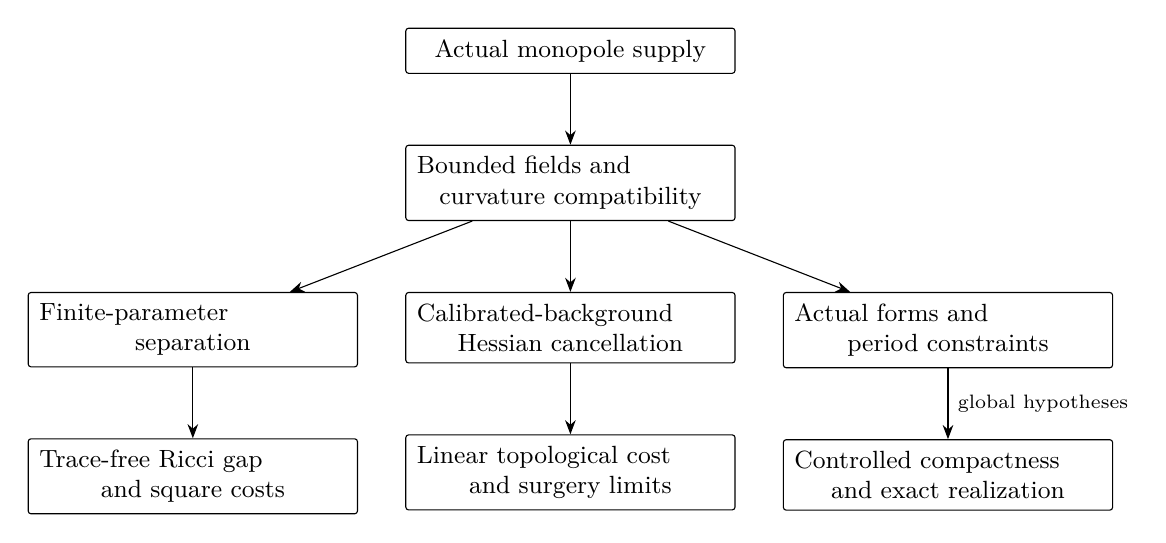
\begin{tikzpicture}[
 node distance=9mm and 6mm,
 box/.style={draw,rounded corners=1pt,align=center,font=\small,
             text width=39mm,inner sep=4pt},
 arr/.style={-{Stealth[length=1.8mm]}}]
\node[box] (supply) {Actual monopole supply};
\node[box,below=of supply] (field) {Bounded fields and\newline curvature compatibility};
\node[box,below left=of field] (parameter) {Finite-parameter\newline separation};
\node[box,below=of field] (linear) {Calibrated-background\newline Hessian cancellation};
\node[box,below right=of field] (forms) {Actual forms and\newline period constraints};
\node[box,below=of parameter] (gap) {Trace-free Ricci gap\newline and square costs};
\node[box,below=of linear] (cost) {Linear topological cost\newline and surgery limits};
\node[box,below=of forms] (real) {Controlled compactness\newline and exact realization};
\draw[arr] (supply)--(field);
\draw[arr] (field)--(parameter);
\draw[arr] (field)--(linear);
\draw[arr] (field)--(forms);
\draw[arr] (parameter)--(gap);
\draw[arr] (linear)--(cost);
\draw[arr] (forms)--node[right,font=\scriptsize]{global hypotheses}(real);
\end{tikzpicture}
\caption{The principal proof dependencies. The realization arrow includes
the global hypotheses stated in the corresponding theorems; it is not
a converse to the obstruction inequalities.}
\end{figure}

The mathematical supplements have six related roles. They retain
arguments not needed for every application of the main inequalities,
without requiring one result to imply all the others.
\begin{center}
\small
\begin{tabularx}{\textwidth}{@{}p{.23\textwidth}X@{}}
\toprule
Geometric question & Results and their relation to the main argument\\
\midrule
Pointwise precursors &
Strict Ricci pinching, polynomial spectral exclusion, and its multiplier
limitation (Section~\ref{sec:early-pointwise-rigidity}); optimized
Ricci-box bounds (Section~\ref{sec:ricci-box-optimization}); local
development and weighted analysis.\\
Simultaneous actual fields &
Harmonic Chern alignment, positive inertia, sign correlation, and
variable Weyl amplitude (Sections~\ref{sec:actual-forms},
\ref{sec:period-inertia}, \ref{sec:joint-matrix},
\ref{sec:variable-calibration}).\\
Compatible geometry &
ALE exclusion and compact realization; bilateral, Chern-boundary,
and finite-cover realization (Sections~\ref{sec:aspherical-cores},
\ref{sec:bilateral}, \ref{sec:chern-boundary},
\ref{sec:virtual-realization}).\\
Global repair &
Uniformly local inversion, integrable cyclic kernels, thin monodromy,
and nonlinear slow fields, each with its stated global hypotheses
(Sections~\ref{sec:local-repair}, \ref{sec:higher-local-repair},
\ref{sec:cyclic-kernel}, \ref{sec:slow-moduli}).\\
Actual degenerating metrics &
Fixed surface bundles, closed shears, canonical classes, and
all-output topological tests (Sections~\ref{sec:fixed-bundle-geometry},
\ref{sec:closed-shear}, \ref{sec:shear-global}); local repair
failure is distinguished from global nonexistence.\\
Marked cores and the weak endpoint &
Whole-filling cost, determinant charge, actual high-index cores,
and signed torsion curvature (Sections~\ref{sec:whole-core},
\ref{sec:marked-charge}, \ref{sec:actual-core-fit},
\ref{sec:quartic-flux}); the remaining endpoint and extremal
questions are stated in Section~\ref{sec:open-problems}.\\
\bottomrule
\end{tabularx}
\end{center}
\clearpage


\clearpage\part{Integral calibration and the parameter theorem}


\section{Intrinsic integral calibration}
\label{sec:intrinsic-calibration}
\hypertarget{proof:intrinsic-calibration:s1}{%
\subsection{Conventions and statements}\label{proof:intrinsic-calibration:s1}}

Let \(M\) be a closed, connected, oriented smooth four-manifold, and let

\[
 V=\operatorname{Vol}_g(M),\qquad T=2\chi(M)+3\tau(M),\qquad
 P=\int_M|\operatorname{Ric}^{\circ}|^2.
\]

Integrals and norms use \(g\), unless stated otherwise. Ricci is a covariant two-tensor; \(W^+\) is the trace-free symmetric curvature endomorphism of \(\Lambda^+\), with its operator Hilbert--Schmidt norm. The Laplacian is nonnegative. Write \(x_-:=\max\{-x,0\}\) and

\[
 4\pi^2T=\int_M\left(\frac{s^2}{24}+2|W^+|^2
                          -\frac{|\operatorname{Ric}^{\circ}|^2}{2}\right).
 \tag{\thesection.1.1}\label{proof:intrinsic-calibration:e1.1}
\]

For a Spin\(^c\) structure with determinant line \(L\), put

\[
 a=c_1(L)\in H^2(M;\mathbb R),\qquad
 a^+=\operatorname{pr}_{H_g^+}a,\qquad p=(a^+)^2.
\]

All cohomological squares mean intersection squares. The quadratic spinor map is normalized by

\[
 |\sigma(\Phi)|^2=|\Phi|^4/8.
\]

\textbf{Definition 1.1 (the conformal monopole hypothesis).} A pair \((g,a)\) satisfies this hypothesis if \(p>0\) and one fixed Spin\(^c\) structure with first Chern class \(a\) has an unperturbed Seiberg--Witten solution for every metric conformal to \(g\). Equivalently for our purposes, for every smooth \(f>0\) there is a solution of

\[
 D_A\Phi=0,\qquad -iF_A^+=f\sigma(\Phi).                 \tag{\thesection.1.2}\label{proof:intrinsic-calibration:e1.2}
\]

The implication from conformal solvability to \eqref{proof:intrinsic-calibration:e1.2} is proved in subsection~\ref{proof:intrinsic-calibration:s2}. The class is not allowed to change as \(f\) changes. A different class may be selected for a different initial metric.

Define the scale-invariant integral Einstein error by

\[
 \mathcal E(g):=\inf_{\lambda\ne0}
  \frac{\int_M|\operatorname{Ric}_g-\lambda g|^2}
       {\lambda^2V}.                                      \tag{\thesection.1.3}\label{proof:intrinsic-calibration:e1.3}
\]

\textbf{Theorem 1.2 (integral rigidity).} There is an absolute constant

\[
                       \varepsilon_0>0                   \tag{\thesection.1.4}\label{proof:intrinsic-calibration:e1.4}
\]

with the following property. Suppose that for a metric \(g\) there is a class \(a\) satisfying Definition 1.1 and

\[
                     (a^+)^2\ge A>0,\qquad a^2\ge T.
 \tag{\thesection.1.5}\label{proof:intrinsic-calibration:e1.5}
\]

Then

\[
 \boxed{\displaystyle
 \mathcal E(g)+\left(\frac TA-\frac23\right)_+
                         \ge\varepsilon_0.}              \tag{\thesection.1.6}\label{proof:intrinsic-calibration:e1.6}
\]

In particular, the conclusion holds for every metric if such a class can be selected metricwise, with the same number \(A\). No regularity of the class selection is needed. The constant is existential and universal; this paper does not assign it a numerical value.

The main analytic ingredient is a calibration gap. Let

\[
 \begin{aligned}
 \mathcal O&=\operatorname{Orb}\operatorname{diag}
                    (-1/6,1/12,1/12)\subset S^2_0(\mathbb R^3),\\
 F&=\operatorname{dist}_{\mathrm{HS}}(W^+,\mathcal O)^2,\qquad
 E=\operatorname{Ric}+g,\qquad e=s+4,\\
 \alpha&=\sqrt{2/3}|W^+|,\qquad q=-s+3\alpha,\\
 \mathcal C&=\int_M(|E|^2+F),\qquad
 \Delta_+=\int_Mq_+^2-72\pi^2p,\\
 \kappa&=(\mathcal C+\Delta_+)/V,\qquad
 B_a=(-a^2)_+/V.
 \end{aligned}                                              \tag{\thesection.1.7}\label{proof:intrinsic-calibration:e1.7}
\]

Here \(\mathcal O\) is interpreted in each oriented orthonormal frame of \(\Lambda^+\); the distance is frame independent.

\textbf{Theorem 1.3 (analytic calibration gap).} Under Definition 1.1,

\[
 \Delta_+\ge0,\qquad (1+B_a)\kappa\ge c_{\mathrm{cal}}>0, \tag{\thesection.1.8}\label{proof:intrinsic-calibration:e1.8}
\]

where \(c_{\mathrm{cal}}\) is absolute.

We prove this theorem first. Throughout the analytic proof, \(C\) denotes an absolute positive constant whose value can change from line to line. Explicit intermediate constants are retained where they clarify the topological transfer, not to advertise an optimized final constant.

\hypertarget{proof:intrinsic-calibration:s2}{%
\subsection{Actual weighted solutions and the retained monopole identities}\label{proof:intrinsic-calibration:s2}}

\hypertarget{proof:intrinsic-calibration:s2.1}{%
\subsubsection{Why the weighted equation has solutions}\label{proof:intrinsic-calibration:s2.1}}

Let \(\widehat g=e^{2u}g=f^{-2}g\), so \(u=-\log f\). Under the fiberwise unitary spinor identification \(\beta\), the conformal formulas are

\[
 \begin{aligned}
 D_A^{\widehat g}(e^{-3u/2}\beta\Phi)
        &=e^{-5u/2}\beta D_A^g\Phi,\\
 \sigma_{\widehat g}(\beta v)&=e^{2u}\sigma_g(v)
                   \quad\hbox{as covariant two-forms}.
 \end{aligned}                                              \tag{\thesection.2.1}\label{proof:intrinsic-calibration:e2.1}
\]

For an ordinary solution \((A,\widehat\Phi)\) for \(\widehat g\), set

\[
                 \Phi=f^{-3/2}\beta^{-1}\widehat\Phi.
\]

Then \(D_A^g\Phi=0\), and

\[
 \sigma_g(\Phi)=f^{-1}\sigma_{\widehat g}(\widehat\Phi).
\]

The Hodge star on two-forms is conformally invariant in dimension four, so the ordinary curvature equation becomes \eqref{proof:intrinsic-calibration:e1.2}. In particular \(H_g^+\) does not change during this operation. This is the conformal weighted monopole construction of \href{https://arxiv.org/pdf/math/0611450}{LeBrun, Lemma 3.7}; the displayed formulas specify the normalization used here.

Set

\[
             \rho=|\Phi|^2,\qquad \psi=2\sqrt2\sigma(\Phi).
 \tag{\thesection.2.2}\label{proof:intrinsic-calibration:e2.2}
\]

Thus \(\psi\) is a smooth self-dual two-form, \(|\psi|=\rho\), and \(\rho\) itself is smooth, including at spinor zeros. The harmonic projection of the determinant curvature gives

\[
 \int_M f^2\rho^2=8\|F_A^+\|_2^2\ge32\pi^2p.           \tag{\thesection.2.3}\label{proof:intrinsic-calibration:e2.3}
\]

Only the squared norm is used, so the equivalent opposite sign convention for the Chern representative does not change this formula.

\hypertarget{proof:intrinsic-calibration:s2.2}{%
\subsubsection{Nonnegative errors}\label{proof:intrinsic-calibration:s2.2}}

The spinor Weitzenböck equation and the self-dual Hodge formula are

\[
 4\nabla_A^*\nabla_A\Phi+(s+f\rho)\Phi=0,                \tag{\thesection.2.4}\label{proof:intrinsic-calibration:e2.4}
\]

\[
 \|d\psi\|_2^2+\|d^*\psi\|_2^2
   =\int_M\left(|\nabla\psi|^2+\frac{s}{3}\rho^2
                                  -2\langle W^+\psi,\psi\rangle\right).
 \tag{\thesection.2.5}\label{proof:intrinsic-calibration:e2.5}
\]

The differential of the Hopf quadratic map in \eqref{proof:intrinsic-calibration:e2.2} satisfies

\[
 |d\psi_z(v)|^2
       =4|z|^2|v|^2-4\bigl(\operatorname{Im}\langle z,v\rangle\bigr)^2
       \le4|z|^2|v|^2.                                   \tag{\thesection.2.6}\label{proof:intrinsic-calibration:e2.6}
\]

The same identity applies covariantly because the map is equivariant and parallel. Pairing \eqref{proof:intrinsic-calibration:e2.4} with \(\rho\Phi\) and integrating yields

\[
 2\int_M|d\rho|^2+4\int_M\rho|\nabla_A\Phi|^2
                  +\int_Ms\rho^2+\int_M f\rho^3=0.       \tag{\thesection.2.7}\label{proof:intrinsic-calibration:e2.7}
\]

Let \(w\) be the smallest eigenvalue of \(W^+\). For a trace-free symmetric three-by-three matrix, \(w\ge-\alpha\). Define

\[
 \begin{aligned}
 D_{\mathrm{amp}}&=2\int_M|d\rho|^2,\\
 D_{\mathrm{quad}}&=\int_M(4\rho|\nabla_A\Phi|^2-|\nabla\psi|^2),\\
 D_H&=\|d\psi\|_2^2+\|d^*\psi\|_2^2=2\|d\psi\|_2^2,\\
 D_{\mathrm{eig}}&=2\int_M
           (\langle W^+\psi,\psi\rangle+\alpha\rho^2),\\
 D_0&=D_{\mathrm{amp}}+D_{\mathrm{quad}}+D_H+D_{\mathrm{eig}}.
 \end{aligned}                                              \tag{\thesection.2.8}\label{proof:intrinsic-calibration:e2.8}
\]

Each term is nonnegative. Equations \eqref{proof:intrinsic-calibration:e2.5}–\eqref{proof:intrinsic-calibration:e2.7} give the exact identity

\[
 D_0=\int_M\left(\frac23q\rho^2-f\rho^3\right).
 \tag{\thesection.2.9}\label{proof:intrinsic-calibration:e2.9}
\]

For \(v=3\rho/2\), this is

\[
                  \int_M(qv^2-fv^3)=\frac{27}{8}D_0.
 \tag{\thesection.2.10}\label{proof:intrinsic-calibration:e2.10}
\]

\hypertarget{proof:intrinsic-calibration:s2.3}{%
\subsubsection{Signed spectral and scalar estimates}\label{proof:intrinsic-calibration:s2.3}}

Put

\[
                  b=2s/3+2w,\qquad h=b_-.
\]

Using \(w\), rather than \(-\alpha\), in \eqref{proof:intrinsic-calibration:e2.5}–\eqref{proof:intrinsic-calibration:e2.7} gives

\[
                       \int_M f\rho^3\le\int_M h\rho^2.
 \tag{\thesection.2.11}\label{proof:intrinsic-calibration:e2.11}
\]

Choose positive smooth functions \(h_j\ge h\) converging uniformly to \(h\), and use the actual solutions with \(f_j=\sqrt{h_j}\). Set

\[
 C_j=\int_M f_j^2\rho^2,\quad Z_j=\int_M f_j\rho^3,
 \quad Q_j=\int_M f_j^4.
\]

Equation \eqref{proof:intrinsic-calibration:e2.11} and Hölder imply

\[
 32\pi^2p\le C_j\le Q_j^{1/3}Z_j^{2/3}
                            \le Q_j^{1/3}C_j^{2/3}.
\]

Consequently \(32\pi^2p\le Q_j\), and uniform approximation proves

\[
 \int_M(2s/3+2w)_-^2\ge32\pi^2p,\qquad
 \int_M q_+^2\ge72\pi^2p.                               \tag{\thesection.2.12}\label{proof:intrinsic-calibration:e2.12}
\]

The second follows from \(b_-\le(2/3)q_+\). This argument passes to a limit of inequalities, not to a limiting spinor or connection.

For \(f=1\), pairing \eqref{proof:intrinsic-calibration:e2.4} with \(\Phi\) gives

\[
 \int_M\rho^2\le\int_Ms_-\rho
        \le\|s_-\|_2\|\rho\|_2.
\]

Together with \eqref{proof:intrinsic-calibration:e2.3}, this proves

\[
                        \int_Ms_-^2\ge32\pi^2p.          \tag{\thesection.2.13}\label{proof:intrinsic-calibration:e2.13}
\]

In particular \(p>0\) excludes a scalar-flat metric. These are the classical monopole curvature estimates in the normalization needed here; the retained terms in \eqref{proof:intrinsic-calibration:e2.8} will supply their quantitative use.

\hypertarget{proof:intrinsic-calibration:s3}{%
\subsection{A bounded spinor with small retained errors}\label{proof:intrinsic-calibration:s3}}

The weights used in subsection~\ref{proof:intrinsic-calibration:s2.3} need not bound the spinor uniformly. For the calibration argument we instead set

\[
       Q=\max\{q,3\},\qquad
       f_0=\max\{\sqrt Q,s_-/4\}.                        \tag{\thesection.3.1}\label{proof:intrinsic-calibration:e3.1}
\]

Choose smooth majorants \(f_j\ge f_0\) with \(f_j\to f_0\) uniformly, and choose an actual solution for each \(f_j\). At a positive maximum of \(\rho\), \eqref{proof:intrinsic-calibration:e2.4} implies \(s+f_j\rho\le0\). Hence

\[
                           0\le\rho\le4,\qquad 0\le v\le6.
 \tag{\thesection.3.2}\label{proof:intrinsic-calibration:e3.2}
\]

All errors \(o_j(1)\) below tend to zero for this fixed smooth metric and fixed class. They require only uniform approximation of \(f_0\), not bounds on derivatives of \(f_j\). No assertion of convergence of the solutions is made.

The two truncations cost only scalar error:

\[
 0\le Q^2-q_+^2\le9e^2,\qquad
 0\le f_0^2-Q\le\frac9{16}e^2.                          \tag{\thesection.3.3}\label{proof:intrinsic-calibration:e3.3}
\]

Indeed, the first difference vanishes unless \(q<3\), which implies \(s>-3\) and \(e>1\). For the second, a nonzero difference implies \(s_->4\sqrt3>6\), and then \(s_-\le3|s+4|\).

Define ideal moments using \(Q\), not the full truncated weight:

\[
 C_*:=\int_M Qv^2,\qquad Z_*:=\int_M\sqrt Qv^3,
 \qquad E_Q:=\int_M Q^2,\qquad P_*:=C_*-Z_*.
 \tag{\thesection.3.4}\label{proof:intrinsic-calibration:e3.4}
\]

Equation \eqref{proof:intrinsic-calibration:e2.10}, \(Q\ge q\), and \(f_j\ge\sqrt Q\) give

\[
 P_*\ge\frac{27}{8}D_0\ge0.                            \tag{\thesection.3.5}\label{proof:intrinsic-calibration:e3.5}
\]

The actual curvature moment is

\[
 C_{\mathrm{act}}:=\int_M f_j^2v^2
                      =18\|F_A^+\|_2^2\ge72\pi^2p.
\]

By \eqref{proof:intrinsic-calibration:e3.2}–\eqref{proof:intrinsic-calibration:e3.3},

\[
 0\le C_{\mathrm{act}}-C_*
                     \le\frac{81}{4}\int_M e^2+o_j(1).
\]

Hölder gives \(C_*\le E_Q^{1/3}Z_*^{2/3}\). Since \(Z_*\le C_*\), it follows that \(C_*\le E_Q\). Thus, with

\[
                        S_*:=\Delta_++\frac{117}{4}\int_Me^2,
\]

we have

\[
                     0\le E_Q-C_*\le S_*+o_j(1).         \tag{\thesection.3.6}\label{proof:intrinsic-calibration:e3.6}
\]

For completeness, two elementary moment inequalities recover all the errors needed below. Write

\[
 \theta=(Z_*/E_Q)^{1/3},\qquad
 H_*=E_Q^{1/3}Z_*^{2/3}-C_*.
\]

Here \(0<\theta\le1\), \(H_*\ge0\), and direct algebra gives

\[
 E_Q-C_*=H_*+\frac{1+\theta}{\theta^2}(P_*+H_*)\ge2P_*.
 \tag{\thesection.3.7}\label{proof:intrinsic-calibration:e3.7}
\]

For the probability measure \(d\nu=Q^2d\mu/E_Q\), let \(r=v/\sqrt Q\), \(c=\int r^2d\nu\), \(z=\int r^3d\nu\), and \(m=\int rd\nu\). We have \(z\le c\le z^{2/3}\), hence \(c\le1\). Also \(c^2\le mz\le mc\), so \(m\ge c\). Therefore

\[
 \int_M Q(v-\sqrt Q)^2=E_Q(c-2m+1)\le E_Q-C_*.
 \tag{\thesection.3.8}\label{proof:intrinsic-calibration:e3.8}
\]

Equations \eqref{proof:intrinsic-calibration:e3.5}–\eqref{proof:intrinsic-calibration:e3.8} prove

\[
 \begin{aligned}
 D_0&\le\frac4{27}S_*+o_j(1),\\
 \int_M|d\rho|^2,\ \int_M|d\psi|^2
     &\le\frac2{27}S_*+o_j(1),\\
 \int_MQ(v-\sqrt Q)^2&\le S_*+o_j(1).
 \end{aligned}                                              \tag{\thesection.3.9}\label{proof:intrinsic-calibration:e3.9}
\]

The point of the ideal moments is that these conclusions do not require any estimate of \(\int f_j^4\), which could be unnecessarily large.

\hypertarget{proof:intrinsic-calibration:s4}{%
\subsection{A globally smooth approximate Weyl tensor}\label{proof:intrinsic-calibration:s4}}

The norm of an element of \(\mathcal O\) is \(1/(2\sqrt6)\). Consequently

\[
 \left\|q-\frac92\right\|_2^2
       \le2\|e\|_2^2+12\int_MF\le12\mathcal C.           \tag{\thesection.4.1}\label{proof:intrinsic-calibration:e4.1}
\]

Clipping at \(3\) moves \(q\) toward \(9/2\), so the same bound holds with \(Q\). Since \(Q\ge3\), \eqref{proof:intrinsic-calibration:e3.8} implies

\[
 \|\rho-\sqrt2\|_2^2
  \le\frac8{27}S_*+\frac2{27}\left\|Q-\frac92\right\|_2^2+o_j(1).
 \tag{\thesection.4.2}\label{proof:intrinsic-calibration:e4.2}
\]

Here the first term follows by writing \(\rho-\sqrt2=(2/3)(v-\sqrt Q)+(2/3)(\sqrt Q-\sqrt{9/2})\) and using \(Q\ge3\).

To estimate direction, choose a measurable rank-one orthogonal projection \(\Pi\) onto a lowest eigenspace of \(W^+\). Then

\[
                  A_0=I/12-\Pi/4
\]

is a nearest point of \(\mathcal O\). On the good set \(F\le1/256\), comparison of ordered eigenvalues with \(A_0\) gives

\[
                   \lambda_2(W^+)-\lambda_1(W^+)\ge1/8.
\]

Putting \(y=(I-\Pi)\psi\), it follows from the eigenvalue error in \eqref{proof:intrinsic-calibration:e2.8} that

\[
 \int_{\{F\le1/256\}}|y|^2\le\frac{16}{27}S_*+o_j(1).
\]

The complementary set has volume at most \(256\int F\), while \(|\psi|^2\le16\). Thus

\[
                 \int_M|y|^2\le\frac{16}{27}S_*+4096\int_MF+o_j(1).
 \tag{\thesection.4.3}\label{proof:intrinsic-calibration:e4.3}
\]

No derivative of \(\Pi\) will be taken. Instead define the polynomial endomorphism

\[
       A_\psi=\frac{\rho^2}{24}I-\frac18\psi\otimes\psi,
             \qquad R=W^+-A_\psi.                       \tag{\thesection.4.4}\label{proof:intrinsic-calibration:e4.4}
\]

It is globally smooth, trace-free, and defined even at spinor zeros. Its eigenvalues are \(-\rho^2/12,\rho^2/24,\rho^2/24\), and \(|A_\psi|^2=\rho^4/96\). The rank-one identity

\[
 |\psi\otimes\psi-\rho^2\Pi|^2=2\rho^2|y|^2
\]

gives the useful comparison

\[
 |A_\psi-A_0|^2
       \le\frac{\rho^2}{16}|y|^2+\frac{(\rho^2-2)^2}{48}.
 \tag{\thesection.4.5}\label{proof:intrinsic-calibration:e4.5}
\]

For example, \eqref{proof:intrinsic-calibration:e4.5} follows by inserting the intermediate matrix \(\rho^2 A_0/2\) and applying \(|X+Y|^2\le2|X|^2+2|Y|^2\). Since \(\rho\le4\) and \((4+\sqrt2)^2<36\), \eqref{proof:intrinsic-calibration:e4.1}–\eqref{proof:intrinsic-calibration:e4.5} imply

\[
 \begin{aligned}
 \|R\|_2^2
 &\le\frac{44}{27}S_*+8194\int_MF
                     +\frac19\left\|Q-\frac92\right\|_2^2+o_j(1)\\
 &\le2\Delta_++8500\mathcal C+o_j(1).
 \end{aligned}                                              \tag{\thesection.4.6}\label{proof:intrinsic-calibration:e4.6}
\]

In the final line we used \(\int e^2\le4\int|E|^2\). In particular, each of

\[
 \|e\|_2^2,\quad\|\rho-\sqrt2\|_2^2,\quad\|R\|_2^2,
            \quad\|d\rho\|_2^2,\quad\|d\psi\|_2^2
\]

is bounded by \(C\kappa V+o_j(1)\).

\hypertarget{proof:intrinsic-calibration:s5}{%
\subsection{A Hessian estimate that needs no Sobolev constant}\label{proof:intrinsic-calibration:s5}}

\textbf{Lemma 5.1.} Let \(u\) be a smooth section of a metric or Hermitian vector bundle with compatible connection over a closed Riemannian four-manifold. Let \(\mathscr F\) be its curvature, with component norm \(\sum_{i,j}|\mathscr F_{ij}|_{\mathrm{HS}}^2\), and set \(K=\|u\|_\infty\). Then

\[
 \begin{aligned}
 \|\nabla u\|_4^2&\le4K\|\nabla^2u\|_2,\\
 \|\nabla^2u\|_2^2
 &\le2\|\nabla^*\nabla u\|_2^2
       +32K^2\|\operatorname{Ric}\|_2^2
       +33K^2\|\mathscr F\|_2^2.
 \end{aligned}                                              \tag{\thesection.5.1}\label{proof:intrinsic-calibration:e5.1}
\]

\textbf{Proof.} Take real parts of Hermitian inner products when necessary. Write \(v_i=\nabla_i u\), \(H_{ij}=\nabla_i v_j\), and \(L=\sum_iH_{ii}=-\nabla^*\nabla u\). Integrating the divergence of \(X_i=|v|^2\langle u,v_i\rangle\) gives

\[
 \int|v|^4
 \le K\int |v|^2(2|H|+|L|)
 \le K\|v\|_4^2(2\|H\|_2+\|L\|_2).
\]

Because \(|L|\le2|H|\) in dimension four, this proves the first inequality, including the case \(\|v\|_4=0\).

For the second, antisymmetry gives

\[
 H_{ij}-H_{ji}=\mathscr F_{ij}u,\qquad
 \|H\|_2^2=\int\langle H_{ij},H_{ji}\rangle
                         +\frac12\sum_{i,j}\|\mathscr F_{ij}u\|_2^2.
 \tag{\thesection.5.2}\label{proof:intrinsic-calibration:e5.2}
\]

The commutator on the bundle-valued one-form \(v\) yields

\[
 \sum_i\nabla_i\nabla_jv_i
     =\nabla_jL+\operatorname{Ric}_{jk}v_k
                                      +\sum_i\mathscr F_{ij}v_i.
\]

Integrating by parts in the first term of \eqref{proof:intrinsic-calibration:e5.2} and using the skew-adjointness of \(\mathscr F_{ij}\), we obtain the exact identity

\[
 \begin{aligned}
 \|H\|_2^2={}&\|L\|_2^2
  -\int\operatorname{Ric}_{ij}\langle v_i,v_j\rangle
  +\sum_{i,j}\int\langle\mathscr F_{ij}v_j,v_i\rangle
  +\frac12\sum_{i,j}\|\mathscr F_{ij}u\|_2^2.
 \end{aligned}                                              \tag{\thesection.5.3}\label{proof:intrinsic-calibration:e5.3}
\]

In particular no derivative of curvature appears. Hölder and the first part bound the middle terms in absolute value by

\[
   4K(\|\operatorname{Ric}\|_2+\|\mathscr F\|_2)\|H\|_2.
\]

Use Young's inequality to absorb half of \(\|H\|_2^2\), and then \((x+y)^2\le2(x^2+y^2)\). This gives exactly the second inequality in \eqref{proof:intrinsic-calibration:e5.1}. No Sobolev inequality or curvature smallness has been used. \(\square\)

\hypertarget{proof:intrinsic-calibration:s5.2}{%
\subsubsection{Applying the lemma to the bounded spinor}\label{proof:intrinsic-calibration:s5.2}}

The calibration budget gives

\[
 \begin{aligned}
 \int|W^+|^2&\le2\int F+V/12,\\
 \int|\operatorname{Ric}|^2&\le2\int|E|^2+8V,\\
 \int s^2&\le8\int|E|^2+32V.
 \end{aligned}                                              \tag{\thesection.5.4}\label{proof:intrinsic-calibration:e5.4}
\]

Equations \eqref{proof:intrinsic-calibration:e3.3} and \eqref{proof:intrinsic-calibration:e4.1} also imply

\[
                         \int f_j^2\le C(V+\mathcal C)+o_j(1).
 \tag{\thesection.5.5}\label{proof:intrinsic-calibration:e5.5}
\]

Indeed \(Q\le9/2+|Q-9/2|\); Cauchy--Schwarz and \(\sqrt{V\mathcal C}\le(V+\mathcal C)/2\) suffice.

For the determinant connection, Chern--Weil and \eqref{proof:intrinsic-calibration:e3.2} give

\[
 \|F_A\|_2^2
   =2\|F_A^+\|_2^2-4\pi^2a^2
   \le4\int f_j^2+4\pi^2(-a^2)_+.
 \tag{\thesection.5.6}\label{proof:intrinsic-calibration:e5.6}
\]

The positive-spinor connection curvature \(\mathscr F_A\) is a fixed linear representation of the Riemannian and determinant curvatures. In the block decomposition of the Riemannian curvature operator, its nontrivial spin action uses the \(\Lambda^+\) output: it sees \(W^+\), \(s\), and the trace-free Ricci block, but not \(W^-\). Consequently \eqref{proof:intrinsic-calibration:e5.4}–\eqref{proof:intrinsic-calibration:e5.6} imply

\[
             \int|\mathscr F_A|^2
               \le C\bigl(V+\mathcal C+(-a^2)_+\bigr)+o_j(1).
 \tag{\thesection.5.7}\label{proof:intrinsic-calibration:e5.7}
\]

From \eqref{proof:intrinsic-calibration:e2.4} and \(\rho\le4\),

\[
 \|\nabla_A^*\nabla_A\Phi\|_2^2
       \le\frac12\int s^2+8\int f_j^2
       \le C(V+\mathcal C)+o_j(1).                        \tag{\thesection.5.8}\label{proof:intrinsic-calibration:e5.8}
\]

Apply Lemma 5.1 with \(\|\Phi\|_\infty\le2\). Since \(A_\psi\) is a parallel polynomial of degree four in \(\Phi\),

\[
 |\nabla^2A_\psi|
      \le C\bigl(|\Phi|^3|\nabla_A^2\Phi|
                               +|\Phi|^2|\nabla_A\Phi|^2\bigr).
\]

We conclude that

\[
 \int\bigl(|\nabla_A^2\Phi|^2+|\nabla_A\Phi|^4
                                      +|\nabla^2A_\psi|^2\bigr)
       \le C\bigl(V+\mathcal C+(-a^2)_+\bigr)+o_j(1).
 \tag{\thesection.5.9}\label{proof:intrinsic-calibration:e5.9}
\]

This proves the required second-derivative budget without differentiating the weight and without an estimate of the anti-self-dual Weyl curvature.

\hypertarget{proof:intrinsic-calibration:s6}{%
\subsection{A weak Bianchi self-test and its incompatible lower bound}\label{proof:intrinsic-calibration:s6}}

\hypertarget{proof:intrinsic-calibration:s6.1}{%
\subsubsection{Tensor normalization and the Bianchi upper bound}\label{proof:intrinsic-calibration:s6.1}}

For an orthonormal basis \(\epsilon_a\) of \(\Lambda^+\), put \(\omega_a=\sqrt2\epsilon_a\). Associate to a symmetric endomorphism \(A\) the four-tensor

\[
 W(A)_{ijkl}=\frac12\sum_{a,b}A_{ab}(\omega_a)_{ij}(\omega_b)_{kl}.
 \tag{\thesection.6.1}\label{proof:intrinsic-calibration:e6.1}
\]

Let

\[
                    J_\psi=\operatorname{div}W(A_\psi),
\]

using the full three-index norm \(\sum_{j,k,l}|J_{jkl}|^2\). Changing the overall sign of divergence changes none of the following squared norms.

The contracted Bianchi identity expresses \(\operatorname{div}W^+\) as a parallel algebraic contraction of \(\nabla\operatorname{Ric}^\circ\) and \(\nabla s\). This follows by contracting the Riemannian Bianchi identity, subtracting the Schouten part, and projecting the final two-form pair onto \(\Lambda^+\); that projection is parallel. Since \(\nabla\operatorname{Ric}=\nabla E\) and \(\nabla s=\nabla\operatorname{tr}E\), integration by parts and \(W(A_\psi)=W^+-W(R)\) show, for every smooth test tensor \(Z\), that

\[
 \left|\int\langle J_\psi,Z\rangle\right|
       \le C(\|E\|_2+\|R\|_2)\|\nabla Z\|_2.
 \tag{\thesection.6.2}\label{proof:intrinsic-calibration:e6.2}
\]

Set \(Z=J_\psi\). It is smooth, and \(\|\nabla J_\psi\|_2\le C\|\nabla^2A_\psi\|_2\). Equations \eqref{proof:intrinsic-calibration:e4.6} and \eqref{proof:intrinsic-calibration:e5.9} therefore give

\[
 \frac1V\int|J_\psi|^2
            \le C\sqrt\kappa\sqrt{1+\kappa+B_a}+o_j(1).
 \tag{\thesection.6.3}\label{proof:intrinsic-calibration:e6.3}
\]

This is a weak identity tested against a smooth tensor already supplied by the spinor. It asserts no pointwise bound on \(\nabla\operatorname{Ric}\).

\hypertarget{proof:intrinsic-calibration:s6.2}{%
\subsubsection{The exact divergence identity}\label{proof:intrinsic-calibration:s6.2}}

Define

\[
 B_\psi=\frac{s}{3}\rho^2-2\langle W^+\psi,\psi\rangle,
 \qquad C_\psi=\langle\iota_{\nabla\rho}\psi,*d\psi\rangle.
\]

We now derive the identity used to lower-bound the left side of \eqref{proof:intrinsic-calibration:e6.3}. Pairing the self-dual Hodge--Weitzenböck equation with \(\rho^2\psi\) and integrating by parts gives

\[
 \int\rho^2\bigl(|\nabla\psi|^2+B_\psi-2|d\psi|^2\bigr)
          =4\int\rho C_\psi-2\int\rho^2|d\rho|^2.
 \tag{\thesection.6.4}\label{proof:intrinsic-calibration:e6.4}
\]

To see the mixed terms explicitly, use \(d^*\psi=-*d\psi\), \(d^*(\rho^2\psi)=\rho^2d^*\psi-2\rho\iota_{\nabla\rho}\psi\), and \(d(\rho^2\psi)=\rho^2d\psi+2\rho d\rho\wedge\psi\). The two exterior-derivative mixed terms add to \(4\rho C_\psi\); the rough-Laplacian mixed term is \(2\rho^2|d\rho|^2\).

The required pointwise first-jet identities are

\[
 |\nabla A_\psi|^2
       =\frac{\rho^2}{32}|\nabla\psi|^2
                                +\frac{\rho^2}{96}|d\rho|^2,
 \tag{\thesection.6.5}\label{proof:intrinsic-calibration:e6.5}
\]

\[
 |\nabla A_\psi|^2-|J_\psi|^2
    =\frac{\rho^2}{64}(|\nabla\psi|^2-2|d\psi|^2)
      +\frac{\rho^2}{32}|d\rho|^2-\frac\rho{16}C_\psi.
 \tag{\thesection.6.6}\label{proof:intrinsic-calibration:e6.6}
\]

Here is a direct component verification that fixes all normalization factors. At a point with \(\rho>0\), choose a parallel orthonormal frame so that

\[
 \begin{aligned}
 \epsilon_1&=(dx^0\wedge dx^1+dx^2\wedge dx^3)/\sqrt2,\\
 \epsilon_2&=(dx^0\wedge dx^2+dx^3\wedge dx^1)/\sqrt2,\\
 \epsilon_3&=(dx^0\wedge dx^3+dx^1\wedge dx^2)/\sqrt2,\\
 \psi&=\rho\epsilon_1,\qquad
 \nabla_m\psi=c_m\epsilon_1+a_m\epsilon_2+b_m\epsilon_3.
 \end{aligned}
\]

Then \(c_m=\partial_m\rho\), and differentiating \eqref{proof:intrinsic-calibration:e4.4} gives

\[
 \nabla_m A_\psi=
 \begin{pmatrix}
  -\rho c_m/6&-\rho a_m/8&-\rho b_m/8\\
  -\rho a_m/8&\rho c_m/12&0\\
  -\rho b_m/8&0&\rho c_m/12
 \end{pmatrix}.                                         \tag{\thesection.6.7}\label{proof:intrinsic-calibration:e6.7}
\]

The squared matrix norm gives \eqref{proof:intrinsic-calibration:e6.5}. For \eqref{proof:intrinsic-calibration:e6.6}, insert \eqref{proof:intrinsic-calibration:e6.7} in \(J_{jkl}=\sum_{m,a,b}(\nabla_mA)_{ab}(\epsilon_a)_{mj}(\epsilon_b)_{kl}\), use \(\sum_{k,l}(\epsilon_b)_{kl}(\epsilon_c)_{kl}=2\delta_{bc}\), and compute \(d\psi_{ijk}=\nabla_i\psi_{jk}+\nabla_j\psi_{ki} +\nabla_k\psi_{ij}\) in the displayed basis. Explicitly,

\[
 *d\psi=\frac1{\sqrt2}
 \begin{pmatrix}
  -a_2-b_3-c_1\\
   a_3-b_2+c_0\\
   a_0+b_1-c_3\\
  -a_1+b_0+c_2
 \end{pmatrix},
 \qquad
 \iota_{\nabla\rho}\psi
       =\frac{\rho}{\sqrt2}(-c_1,c_0,-c_3,c_2).
\]

These expressions and \eqref{proof:intrinsic-calibration:e6.7} give \eqref{proof:intrinsic-calibration:e6.6} by summing squares and collecting the mixed terms in \(C_\psi\). Thus \eqref{proof:intrinsic-calibration:e6.5}–\eqref{proof:intrinsic-calibration:e6.6} are algebraic identities in the twelve arbitrary numbers \(c_m,a_m,b_m\), with no field equation imposed. At a spinor zero, both \(\psi\) and its first derivative vanish, and \(d\rho=0\); the identities extend there as well.

Combining \eqref{proof:intrinsic-calibration:e6.4}–\eqref{proof:intrinsic-calibration:e6.6} eliminates \(\int\rho^2|\nabla\psi|^2\) and gives

\[
 \begin{aligned}
 \int|J_\psi|^2={}&-\frac1{64}\int\rho^2 B_\psi
       +\frac1{16}\int\rho^2|d\psi|^2
       -\frac5{96}\int\rho^2|d\rho|^2
       +\frac18\int\rho C_\psi.
 \end{aligned}                                              \tag{\thesection.6.8}\label{proof:intrinsic-calibration:e6.8}
\]

\hypertarget{proof:intrinsic-calibration:s6.3}{%
\subsubsection{The positive lower bound and contradiction}\label{proof:intrinsic-calibration:s6.3}}

Because \(A_\psi\psi=-\rho^2\psi/12\), the curvature term in \eqref{proof:intrinsic-calibration:e6.8} is

\[
 -\frac{\rho^2B_\psi}{64}
        =-\frac{s\rho^4}{192}-\frac{\rho^6}{384}
                                +\frac{\rho^2\langle R\psi,\psi\rangle}{32}.
 \tag{\thesection.6.9}\label{proof:intrinsic-calibration:e6.9}
\]

At \(s=-4\), \(\rho=\sqrt2\), and \(R=0\), it equals \(1/16\). On the interval \(0\le\rho\le4\), the error in \eqref{proof:intrinsic-calibration:e6.9} is bounded by

\[
                  C\bigl(|e|+|\rho-\sqrt2|+|R|\bigr).
\]

Also \(|C_\psi|\le\rho|d\rho||d\psi|\). Discard the nonnegative \(|d\psi|^2\) term in \eqref{proof:intrinsic-calibration:e6.8}, apply \eqref{proof:intrinsic-calibration:e3.9}, \eqref{proof:intrinsic-calibration:e4.2}, and \eqref{proof:intrinsic-calibration:e4.6}, and divide by \(V\). Cauchy--Schwarz gives

\[
 \frac1V\int|J_\psi|^2
                   \ge\frac1{16}-C(\sqrt\kappa+\kappa)+o_j(1).
 \tag{\thesection.6.10}\label{proof:intrinsic-calibration:e6.10}
\]

For each fixed metric let the smooth-weight approximation errors tend to zero in \eqref{proof:intrinsic-calibration:e6.3} and \eqref{proof:intrinsic-calibration:e6.10}. The two numerical inequalities remain valid without choosing any limit of the spinors. For a sufficiently small absolute \(\kappa_0\le1\), the lower bound is at least \(1/32\) when \(\kappa\le\kappa_0\). The upper bound then forces

\[
                         \kappa(1+\kappa+B_a)\ge c_1>0.
\]

As \(1+\kappa+B_a\le2(1+B_a)\) in this range, \eqref{proof:intrinsic-calibration:e1.8} follows. For \(\kappa>\kappa_0\), it follows after decreasing the same universal constant. This proves Theorem 1.3. \(\square\)

\hypertarget{proof:intrinsic-calibration:s7}{%
\subsection{From the calibration gap to topological integral rigidity}\label{proof:intrinsic-calibration:s7}}

We now prove Theorem 1.2, first at the negative normalization. Assume \eqref{proof:intrinsic-calibration:e1.5}, and put

\[
 r=\frac1V\int|\operatorname{Ric}+g|^2,\qquad
 d=\left(\frac TA-\frac23\right)_+.
\]

Continue to use \(\alpha=\sqrt{2/3}|W^+|\) and \(w=\lambda_{\min}(W^+)\), and introduce

\[
 t=s+24\alpha=s+8\sqrt6|W^+|,\qquad
 b=2s/3+2w,\qquad
 G=(2s/3-2\alpha)^2-b_-^2.                               \tag{\thesection.7.1}\label{proof:intrinsic-calibration:e7.1}
\]

Since \(b\ge2s/3-2\alpha\), we have \(G\ge0\), including where the scalar curvature is positive. Direct expansion gives

\[
 t^2+18G=216\left(s^2/24+2|W^+|^2\right)-18b_-^2.
\]

Apply \eqref{proof:intrinsic-calibration:e1.1} and \eqref{proof:intrinsic-calibration:e2.12} to obtain

\[
                    \int(t^2+18G)\le108P+864\pi^2Ad.
 \tag{\thesection.7.2}\label{proof:intrinsic-calibration:e7.2}
\]

Here \(p\ge A\) and \(T-2p/3\le T-2A/3\le Ad\). Since \(\int|E|^2=P+\frac14\int e^2\), \eqref{proof:intrinsic-calibration:e7.2} implies

\[
             \int(|E|^2+e^2+t^2+G)\le109rV+864\pi^2Ad.
 \tag{\thesection.7.3}\label{proof:intrinsic-calibration:e7.3}
\]

We record the pointwise orbit comparison, including its scalar-positive branch. Set \(z=w+\alpha\); trace-freeness gives \(0\le z\le\alpha\), and minimizing over the orbit gives exactly

\[
 F=\frac32(\alpha-1/6)^2+z/2,\qquad
                         \alpha=(t-e+4)/24.              \tag{\thesection.7.4}\label{proof:intrinsic-calibration:e7.4}
\]

If \(s\le-3\), then \(b<0\) and \(G=z(-8s/3+8\alpha-4z)\ge8z\). Thus

\[
                       F\le(t^2+e^2)/192+G/16.
\]

If \(s>-3\), then \(e>1\). Use \(z\le\alpha\), \(4-e\le3e^2\), and \(t\le(t^2+1)/2\) in \eqref{proof:intrinsic-calibration:e7.4} to get

\[
                       F\le(t^2+5e^2)/64.
\]

In both cases,

\[
                             F\le e^2+t^2+G.             \tag{\thesection.7.5}\label{proof:intrinsic-calibration:e7.5}
\]

The second completed square is

\[
 27\left(s^2/24+2|W^+|^2\right)-q^2=t^2/8.
\]

It and \eqref{proof:intrinsic-calibration:e1.1} yield

\[
 \Delta_+\le\frac{27}{2}rV+108\pi^2Ad.
\]

Combining this with \eqref{proof:intrinsic-calibration:e7.3}–\eqref{proof:intrinsic-calibration:e7.5},

\[
                     \kappa\le\frac{245}{2}r
                                      +972\pi^2\frac AVd.
 \tag{\thesection.7.6}\label{proof:intrinsic-calibration:e7.6}
\]

The scalar estimate \eqref{proof:intrinsic-calibration:e2.13} gives

\[
 32\pi^2A\le\int s^2\le32V+8rV,
              \qquad \frac AV\le\frac{4+r}{4\pi^2}.
 \tag{\thesection.7.7}\label{proof:intrinsic-calibration:e7.7}
\]

For \(r\le1\), therefore,

\[
                              \kappa\le1215(r+d).        \tag{\thesection.7.8}\label{proof:intrinsic-calibration:e7.8}
\]

When \(r\le1/4\), reverse triangle inequality in \(L^2\) and \eqref{proof:intrinsic-calibration:e1.1} also imply

\[
 4\pi^2T
     \ge\left[\frac{(4-2\sqrt r)^2}{24}-\frac r2\right]V
     \ge V/4>0.                                          \tag{\thesection.7.9}\label{proof:intrinsic-calibration:e7.9}
\]

The square condition \(a^2\ge T\) then gives \(B_a=0\). Apply Theorem 1.3 and \eqref{proof:intrinsic-calibration:e7.8}. If \(r>1/4\), no argument is needed. In either case

\[
       r+d\ge\varepsilon_0,
       \qquad \varepsilon_0:=\min\{1/4,c_{\mathrm{cal}}/1215\}.
 \tag{\thesection.7.10}\label{proof:intrinsic-calibration:e7.10}
\]

For reference, a weaker square hypothesis has a correspondingly nonuniversal version. If \(a^2\ge-C_AA\), \(C_A\ge0\), the same proof gives

\[
 r+d\ge\min\left\{1,
          \frac{c_{\mathrm{cal}}}{1215(1+5C_A/(4\pi^2))}\right\}.
 \tag{\thesection.7.11}\label{proof:intrinsic-calibration:e7.11}
\]

If instead \(a^2\ge T-C_AA\), replace the first entry of that minimum by \(1/4\), using \eqref{proof:intrinsic-calibration:e7.9}. An arbitrary monopole class must not silently be assumed to have \(a^2\ge T\).

\hypertarget{proof:intrinsic-calibration:s8}{%
\subsection{Positive scale, arbitrary scale, and the Ricci-flat case}\label{proof:intrinsic-calibration:s8}}

\hypertarget{proof:intrinsic-calibration:s8.1}{%
\subsubsection{The positive normalization}\label{proof:intrinsic-calibration:s8.1}}

Put \(r_+=V^{-1}\int|\operatorname{Ric}-g|^2\). Since \(s_-^2\le(s-4)^2\le4|\operatorname{Ric}-g|^2\), \eqref{proof:intrinsic-calibration:e2.13} gives

\[
                            A/V\le r_+/(8\pi^2).
\]

If \(r_+\le1/4\), the analogue of \eqref{proof:intrinsic-calibration:e7.9} gives \(4\pi^2T/V\ge1/4\). If also \(d\le1/4\), then \(T/A\le2/3+d\), so

\[
  \frac14\le\frac{4\pi^2T}{V}
             \le\frac{r_+}{2}\left(\frac23+d\right)
             \le\frac{11}{96},
\]

a contradiction. In particular \(r_++d>1/4\).

\hypertarget{proof:intrinsic-calibration:s8.2}{%
\subsubsection{Scale optimization}\label{proof:intrinsic-calibration:s8.2}}

For \(\lambda\ne0\), apply the appropriate normalized result to \(|\lambda|g\). The positive harmonic subspace and the conformal solvability hypothesis are unchanged. The normalized error becomes

\[
 \frac{\int|\operatorname{Ric}_g-\lambda g|^2}{\lambda^2V}.
\]

Taking the infimum proves \eqref{proof:intrinsic-calibration:e1.6}. This completes Theorem 1.2. \(\square\)

For interpretation, write

\[
 R_2=\int|\operatorname{Ric}|^2,\qquad S=\int s,\qquad
 L_s=\int(s-S/V)^2.
\]

When \(R_2>0\), direct minimization in \(1/\lambda\) gives

\[
              \mathcal E(g)=4-\frac{S^2}{VR_2}
                             =\frac{4P+L_s}{R_2}.        \tag{\thesection.8.1}\label{proof:intrinsic-calibration:e8.1}
\]

This formula includes \(S=0\), when the infimum is \(4\) and need not be attained. If \(R_2=0\), definition \eqref{proof:intrinsic-calibration:e1.3} gives \(\mathcal E(g)=4\), not zero. Thus a lower bound for \(\mathcal E\) alone does not exclude a Ricci-flat metric. Ricci-flat metrics in Theorem 1.2 are excluded separately by \eqref{proof:intrinsic-calibration:e2.13}, since \(p\ge A>0\).

For an Einstein metric with nonzero Einstein constant, \(\mathcal E=0\). A pointwise operator error also dominates the integral one: for \(\sigma=\pm1\),

\[
 \delta_\sigma(g):=\|\operatorname{Ric}^{\sharp}-\sigma I\|_{L^\infty,\mathrm{op}}
      \quad\Longrightarrow\quad\mathcal E(g)\le4\delta_\sigma(g)^2.
 \tag{\thesection.8.2}\label{proof:intrinsic-calibration:e8.2}
\]

There are exactly four Ricci eigenvalues, which explains this factor.

\hypertarget{proof:intrinsic-calibration:s9}{%
\subsection{Metricwise polarized classes and chamber bookkeeping}\label{proof:intrinsic-calibration:s9}}

The analytic theorem needs the quantifiers

\[
 \boxed{\begin{gathered}
   \text{for every }g\text{ there exists a Spin}^c
       \text{ structure }\mathfrak s_g\\
   \text{such that for every }f>0,\text{ equation (1.2)}\\
   \text{has a solution for the same }\mathfrak s_g.
 \end{gathered}}
 \tag{\thesection.9.1}\label{proof:intrinsic-calibration:e9.1}
\]

It does not require one universal choice of signs for all metrics. This distinction is essential when \(b_+=1\).

\hypertarget{proof:intrinsic-calibration:s9.1}{%
\subsubsection{The connected-sum input with insertions}\label{proof:intrinsic-calibration:s9.1}}

Let \(X\) have \(b_+(X)>0\), and suppose a Spin\(^c\) structure \(\mathfrak s\), with real first Chern class \(c\), has a nonzero Seiberg--Witten invariant evaluated on a homogeneous insertion \(z\). The invariant is defined on

\[
 \mathbb A(X)=\mathbb Z[U]\otimes\Lambda^*H_1(X;\mathbb Z)/\mathrm{torsion},
                 \qquad\deg U=2,\quad\deg H_1=1.
\]

Its expected dimension is \((c^2-T_X)/4\), where \(T_X=2\chi(X)+3\tau(X)\). Assume

\[
                    T_X>0,\qquad A:=c^2\ge T_X.          \tag{\thesection.9.2}\label{proof:intrinsic-calibration:e9.2}
\]

The second inequality follows automatically from the nonnegative degree of a nonzero ordinary invariant, but is displayed because it is used in the proof. For \(b_+=1\), the nonzero invariant here must be in the small-perturbation chamber at the relevant polarization, not merely in some unspecified chamber.

Let

\[
 M=X\#k\,\overline{\mathbb{CP}}^{2}\#\ell(S^1\times S^3),
 \qquad D=k+4\ell,\qquad T_M=T_X-D.                      \tag{\thesection.9.3}\label{proof:intrinsic-calibration:e9.3}
\]

For a prescribed positive polarization \(H=H_g^+\), choose the signs of the exceptional generators \(E_j\) so that

\[
                         c_H^+\mathbin\cdot E_j\le0,
\]

and set

\[
                             a_H=c-\sum_{j=1}^kE_j.
 \tag{\thesection.9.4}\label{proof:intrinsic-calibration:e9.4}
\]

Then

\[
 \begin{aligned}
 (a_H^+)^2
   &=(c_H^+)^2-2\sum_jc_H^+\mathbin\cdot E_j
                              +\left|\sum_j(E_j)_H^+\right|^2
      \ge(c_H^+)^2\ge c^2=A,\\
 a_H^2&=A-k\ge T_X-k-4\ell=T_M.
 \end{aligned}                                              \tag{\thesection.9.5}\label{proof:intrinsic-calibration:e9.5}
\]

The ordinary blow-up formula with exceptional coefficient \(\pm1\) preserves expected dimension and preserves the original insertion \(z\). The \(S^1\times S^3\) operation raises expected dimension by one and adds the degree-one insertion of its new circle. After \(\ell\) operations the nonzero invariant is therefore evaluated on

\[
                           z\,\mu(C_1)\cdots\mu(C_\ell).
 \tag{\thesection.9.6}\label{proof:intrinsic-calibration:e9.6}
\]

These statements include positive-dimensional base invariants. They are the special cases of the blow-up and surgery formulas in \href{https://arxiv.org/pdf/math/0005268}{Ozsváth--Szabó, Theorem 3.2, Proposition 2.2 and Remark 2.3}. The last remark supplies the chamber-compatible version when \(b_+=1\). Using only a zero-dimensional numerical invariant and omitting the insertions in \eqref{proof:intrinsic-calibration:e9.6} would not justify the general statement.

\hypertarget{proof:intrinsic-calibration:s9.2}{%
\subsubsection{What the chamber condition means}\label{proof:intrinsic-calibration:s9.2}}

For \(b_+(X)=1\), choose a unit forward generator \(\omega_H\) of the positive line on \(M\) so that \(c\cdot\omega_H>0\). The \(X\) component \(\omega_X\) has positive square, lies in the corresponding forward cone, and satisfies \(c\cdot\omega_X>0\), because \(c^2>0\). The chosen exceptional signs give \(E_j\cdot\omega_H\le0\), hence

\[
                          a_H\cdot\omega_H>0.             \tag{\thesection.9.7}\label{proof:intrinsic-calibration:e9.7}
\]

Thus the small-perturbation discriminants for the base and the selected blow-up structure have the same sign in corresponding chamber conventions. Adding \(S^1\times S^3\) leaves the second-cohomology polarization unchanged. The gluing formulas consequently give a nonzero invariant in the chamber containing zero perturbation for this selected class, provided that was the specified nonzero base chamber.

For any metric with this polarization, take generic perturbations tending to zero in that chamber. Nonzero invariant gives solutions, and the usual fixed-metric Seiberg--Witten compactness gives an unperturbed solution. A reducible limit would have \(F_A^+=0\), contradicting \((a_H^+)^2\ge A>0\). Every metric conformal to \(g\) has the same polarization and the same nonzero discriminant sign. Thus the \emph{same} class \eqref{proof:intrinsic-calibration:e9.4} satisfies Definition 1.1 for every weight, as required by \eqref{proof:intrinsic-calibration:e9.1}.

For \(b_+>1\), there is no chamber ambiguity in this argument. For \(b_+=1\), the statement must not be replaced by the assertion that every exceptional sign choice is an ordinary all-metric monopole class.

\hypertarget{proof:intrinsic-calibration:s9.3}{%
\subsubsection{The minimal general-type case}\label{proof:intrinsic-calibration:s9.3}}

If \(X\) is a minimal compact complex surface of general type with its complex orientation, then

\[
                          A=c_1(X)^2=T_X>0.
\]

The canonical Spin\(^c\) structure has a nonzero Seiberg--Witten invariant. For \(b_+>1\), the standard Kähler/symplectic nonvanishing statement supplies the input directly. For \(b_+=1\), the canonical class \(K\) has \(K^2>0\) and positive pairing with a Kähler form. It is therefore in the forward time-like cone and pairs positively with every forward period ray. For \(c=-K\), the small-perturbation chamber agrees with the canonical nonzero chamber, up to the simultaneous choice of sign convention for the chamber discriminant. This is the light-cone/chamber argument underlying \href{https://arxiv.org/pdf/math/0003068}{LeBrun's polarized construction, Proposition 3.2}. The chamber convention and canonical nonvanishing can also be read in \href{https://arxiv.org/pdf/math/0012048}{Li--Liu, §2.1 and Theorem 2.2}.

The positivity of \(K\) on the symplectic or Kähler form matters: \(b_+=1\) and \(K^2>0\) alone do not identify the nonzero small-perturbation chamber for an arbitrary symplectic manifold.

\hypertarget{proof:intrinsic-calibration:s10}{%
\subsection{The Einstein obstruction and its precise relation to LeBrun}\label{proof:intrinsic-calibration:s10}}

\textbf{Theorem 10.1 (connected-sum integral obstruction).} Under the gauge-theoretic and chamber assumptions of subsection~\ref{proof:intrinsic-calibration:s9.1}, every metric on \eqref{proof:intrinsic-calibration:e9.3} satisfies

\[
 \mathcal E(g)+\left(\frac{T_M}{A}-\frac23\right)_+
                         \ge\varepsilon_0.               \tag{\thesection.10.1}\label{proof:intrinsic-calibration:e10.1}
\]

It also satisfies the slightly weaker but base-topological statement

\[
 \boxed{\displaystyle
 \mathcal E(g)+\left(\frac13-\frac{D}{T_X}\right)_+
                         \ge\varepsilon_0.}              \tag{\thesection.10.2}\label{proof:intrinsic-calibration:e10.2}
\]

For minimal general type, \(A=T_X=c_1(X)^2\), so the two statements coincide.

\textbf{Proof.} Equation \eqref{proof:intrinsic-calibration:e9.5} and the conformal solvability just proved give all the hypotheses of Theorem 1.2. If \(T_M>0\), then \(A\ge T_X\) implies \(T_M/A\le T_M/T_X\), yielding \eqref{proof:intrinsic-calibration:e10.2}. If \(T_M\le0\), both positive-part terms are zero. This case split avoids reversing an inequality by dividing a negative numerator by the larger denominator. \(\square\)

In particular, put \(\gamma=\varepsilon_0/2\). Then

\[
             D\ge(1/3-\gamma)T_X
 \quad\Longrightarrow\quad
             \mathcal E(g)\ge\varepsilon_0/2
             \quad\hbox{for every metric }g.             \tag{\thesection.10.3}\label{proof:intrinsic-calibration:e10.3}
\]

There is no Einstein metric in this band: nonzero Einstein constants contradict \eqref{proof:intrinsic-calibration:e10.3}, and zero Einstein constant contradicts \eqref{proof:intrinsic-calibration:e2.13}. At either normalized sign, \eqref{proof:intrinsic-calibration:e8.2} also gives

\[
                    \delta_\sigma(g)\ge\sqrt{\varepsilon_0/8}.
 \tag{\thesection.10.4}\label{proof:intrinsic-calibration:e10.4}
\]

An Einstein metric would in fact require \(D/T_X\le1/3-\varepsilon_0\). The equality endpoint of that necessary condition is not excluded by \eqref{proof:intrinsic-calibration:e10.2} alone; the closed band \eqref{proof:intrinsic-calibration:e10.3} avoids that endpoint issue.

\hypertarget{proof:intrinsic-calibration:s10.2}{%
\subsubsection{Exact source scope}\label{proof:intrinsic-calibration:s10.2}}

The version of \href{https://arxiv.org/pdf/math/0003068}{LeBrun's preprint} is arXiv:math/0003068v1, March 2000. Its Proposition 3.2 constructs the metricwise polarized classes on the connected sums in \eqref{proof:intrinsic-calibration:e9.3}. Its Theorem 3.3 states the classical threshold

\[
                              k+4\ell\ge T_X/3,
\]

and Corollary 3.4 specializes the result to blow-ups of minimal complex surfaces of general type. We use the ordinary nontrivial Seiberg--Witten input, including its insertion and chamber meaning, not merely the topology of a manifold with the same Euler characteristic and signature. The proof above handles the positive-budget case of the general theorem, not only its general-type corollary.

The numerical band below the classical threshold is nonvacuous in families with unbounded budget. For example, let \(X_m=\Sigma_2\times\Sigma_m\), \(m\ge2\). Then \(A=T_{X_m}=8(m-1)\). With \(\ell=0\) and \(k=\lceil A/3\rceil-1\),

\[
                       0<1/3-k/A\le1/A\longrightarrow0.
\]

For sufficiently large \(m\), these ratios lie in \eqref{proof:intrinsic-calibration:e10.3}. Since the universal analytic constant has not been made numerical, this argument does not specify the first qualifying \(m\).

\hypertarget{proof:intrinsic-calibration:s10.3}{%
\subsubsection{Nonpositive budgets and the exceptional zero corner}\label{proof:intrinsic-calibration:s10.3}}

There is a direct all-metric formula, independent of monopoles. For \(R_2>0\), \eqref{proof:intrinsic-calibration:e1.1} and \eqref{proof:intrinsic-calibration:e8.1} give

\[
 \mathcal E(g)
   =1+\frac{12\int|W^+|^2-24\pi^2T+L_s}{R_2}.           \tag{\thesection.10.5}\label{proof:intrinsic-calibration:e10.5}
\]

Thus \(T\le0\) implies \(\mathcal E(g)\ge1\). For a Ricci-flat metric its value is \(4\) by definition, so the same lower bound holds. This lower bound is not a Ricci-flat exclusion.

For an Einstein metric, \eqref{proof:intrinsic-calibration:e1.1} reduces to

\[
               4\pi^2T=\int(s^2/24+2|W^+|^2)\ge0.
\]

Consequently, when \(T_X<0\), or when \(T_X=0\) and \(D>0\), the connected sum has \(T_M<0\) and admits no Einstein metric. These are classical Chern--Gauss--Bonnet consequences and require no positive-budget monopole argument.

When \(T_X=D=0\), however, equality permits Ricci-flat, anti-self-dual metrics in the chosen orientation. K3 and the four-torus provide the standard zero-budget examples. Thus the positive-budget integral strengthening and the negative-\(T_M\) exclusion must be distinguished from the Ricci-flat zero corner.


\section{A differential criterion for bounded self-dual forms}
\label{sec:bounded-forms}
\hypertarget{proof:bounded-forms:s1}{%
\subsection{The bounded two-form criterion}\label{proof:bounded-forms:s1}}

For a smooth self-dual two-form \(\psi\), set

\[
 q=|\psi|^2,\qquad
 A_\psi={q\over24}I-{1\over8}\psi\otimes\psi,
 \qquad R=W^+-A_\psi.
\]

Define the defect and source budget

\[
 d=\fint_M\left(|\operatorname{Ric}+g|^2+|R|^2+(q-2)^2\right),
 \qquad B=\fint_M|\Delta_H\psi|^2.
\]

\textbf{Theorem.} For each finite \(K>0\), there is \(c(K)>0\) such that \(\|\psi\|_\infty\le K\) implies

\[
                    \boxed{(1+B)d\ge c(K).}              \tag{\thesection.1}\label{proof:bounded-forms:e1}
\]

\textbf{Small-source corollary.} For a possibly smaller \(c_0(K)>0\),

\[
 \boxed{\quad
 \fint_M\left(
 |\operatorname{Ric}+g|^2+|R|^2+(q-2)^2+|\Delta_H\psi|^2
 \right)\ge c_0(K).
 \quad}                                                     \tag{\thesection.1a}\label{proof:bounded-forms:e1a}
\]

No spin structure, monopole class, curvature bound, scalar sign, Sobolev constant, injectivity radius or diameter bound is required. In particular, for bounded \emph{harmonic} self-dual forms \(B=0\), giving a gap for the three zeroth-order defects alone. No small first-derivative defect is assumed, even in the nonharmonic case. The boundedness of the form and its Hodge-Laplacian control are genuine hypotheses, not consequences of a cohomology class alone.

The theorem excludes a specific incompatible calibration: Ricci curvature near \(-g\), Weyl curvature near \(A_\psi\), and \(|\psi|^2\) near two. For a product of curvature-minus-one surfaces the simple Weyl eigenvalue is \(-2/3\), not the target \(-1/6\). Thus the theorem does not exclude the realizable hyperbolic-product Weyl model and does not assert a universal Ricci gap without the other summands.

\hypertarget{proof:bounded-forms:s2}{%
\subsection{Re-derivation of the bundle Hessian estimate}\label{proof:bounded-forms:s2}}

Let \(u\) be a smooth section of a metric bundle, with compatible connection \(\nabla\). Set \(H_{ij}=\nabla_i\nabla_j u\), including the cotangent Levi-Civita correction, \(L=\operatorname{tr}H\), and \(F_{ij}=[\nabla_i,\nabla_j]\). Use the component convention \(|F|^2=\sum_{ij}|F_{ij}|_{\rm HS}^2\).

First, integration of the divergence of \(|\nabla u|^2\langle u,\nabla u\rangle^\sharp\) gives

\[
 \|\nabla u\|_4^2\le(2+\sqrt4)\|u\|_\infty\|H\|_2.
                                                               \tag{\thesection.2}\label{proof:bounded-forms:e2}
\]

This is a covariant integration-by-parts inequality, not a Sobolev embedding. To check the curvature terms, first interchange the two Hessian slots:

\[
 \int|H|^2-\sum_{ij}\int\langle H_{ij},H_{ji}\rangle
 =\frac12\sum_{ij}\int|F_{ij}u|^2.
\]

Integrate the second expression once and then commute derivatives on the bundle-valued one-form \(\nabla u\). The cotangent curvature gives Ricci; the bundle curvature acts on \(\nabla u\). Integrating the trace term once more yields

\[
\begin{aligned}
 \int|H|^2={}&\int|L|^2
 -\int\operatorname{Ric}_{ij}\langle\nabla_i u,\nabla_j u\rangle\\
 &+\sum_{ij}\int\langle F_{ij}\nabla_j u,\nabla_i u\rangle
 +\frac12\sum_{ij}\int|F_{ij}u|^2.
\end{aligned}\tag{\thesection.3}\label{proof:bounded-forms:e3}
\]

There is no differentiated-curvature term. Swapping the Hessian slots \emph{before} commuting is important. The scalar specialization fixes the Ricci sign. With \(K_u=\|u\|_\infty\), Holder, \eqref{proof:bounded-forms:e2}, and Young give

\[
 \|\nabla^2u\|_2^2\le
 2\|L\|_2^2+32K_u^2\|\operatorname{Ric}\|_2^2
                         +33K_u^2\|F\|_2^2.              \tag{\thesection.4}\label{proof:bounded-forms:e4}
\]

This recovers the estimate, including its coefficient and the absence of a hidden Sobolev or curvature-derivative hypothesis.

\hypertarget{proof:bounded-forms:s3}{%
\subsection{Proof of the two-form criterion}\label{proof:bounded-forms:s3}}

Assume \(d\le1\); otherwise the conclusion is immediate after reducing \(c(K)\). Put \(\mathcal B=1+B+d\). All constants below depend only on \(K\) and the dimension. Put \(E=\operatorname{Ric}+g\) and \(\eta=\Delta_H\psi\).

\hypertarget{proof:bounded-forms:s3.1}{%
\subsubsection{The self-dual connection supplies the second-order budget}\label{proof:bounded-forms:s3.1}}

The curvature of \(\Lambda^+\) is the representation of the Riemann operator projected to its self-dual output. Hence

\[
 |F^{\Lambda^+}|^2\le C\left(|W^+|^2+s^2+
                               |\operatorname{Ric}^{\circ}|^2\right).
                                                               \tag{\thesection.5}\label{proof:bounded-forms:e5}
\]

The \(W^-\) block does not act on \(\Lambda^+\). Since \(|A_\psi|^2=q^2/96\) and \(q\le K^2\), the \(E,R\) budgets give

\[
 \fint\left(|\operatorname{Ric}|^2+|F^{\Lambda^+}|^2\right)
 \le C_K(1+d).
\]

The self-dual Weitzenbock equation is

\[
 \nabla^*\nabla\psi=\eta+2W^+\psi-(s/3)\psi.
\]

Apply \eqref{proof:bounded-forms:e2}–\eqref{proof:bounded-forms:e4} to \(u=\psi\). Differentiating the quadratic polynomial \(A_\psi\) and the scalar \(q\) then gives

\[
 \fint\left(|\nabla^2\psi|^2+|\nabla\psi|^4+
              |\nabla^2A_\psi|^2+|\Delta q|^2\right)
 \le C_K\mathcal B.
                                                               \tag{\thesection.6}\label{proof:bounded-forms:e6}
\]

Here \(\Delta=d^*d\) on functions, and \(\Delta q=2\langle\nabla^*\nabla\psi,\psi\rangle -2|\nabla\psi|^2\). All estimates are extensive before division by volume; no lower volume bound enters.

\hypertarget{proof:bounded-forms:s3.2}{%
\subsubsection{Amplitude control and a coercive divergence identity}\label{proof:bounded-forms:s3.2}}

The amplitude itself need not have a smooth square root at its zeros. Use the globally smooth quantity \(q\), rather than divide by \(|\psi|\). Integration by parts and \eqref{proof:bounded-forms:e6} give

\[
 \fint|dq|^2=\fint(q-2)\Delta q
                  \le C_K\sqrt{d\mathcal B}.             \tag{\thesection.7}\label{proof:bounded-forms:e7}
\]

There is a useful pointwise identity, valid for arbitrary smooth self-dual forms without first-order equations. Let \(J=\operatorname{div}W(A_\psi)\). Direct contraction gives

\[
 |J|^2={q|\nabla\psi|^2\over64}+{q|d\psi|^2\over32}
       -{|dq|^2\over192}
       +{\langle\iota_{\nabla q}\psi,*d\psi\rangle\over32}.
                                                               \tag{\thesection.8}\label{proof:bounded-forms:e8}
\]

The last inner product is at most \(\sqrt q\,|dq|\,|d\psi|\) in absolute value. Young's inequality therefore gives the pointwise coercivity

\[
 \boxed{\quad
 q\bigl(|\nabla\psi|^2+|d\psi|^2\bigr)
        \le64|J|^2+{4\over3}|dq|^2.
 \quad}                                                     \tag{\thesection.8a}\label{proof:bounded-forms:e8a}
\]

This is polynomial at zeros, and introduces no division by \(q\). It will control the derivative terms for the two-sided selection theorem in subsection~\ref{proof:bounded-forms:s6}. Small amplitude error and a second-order budget now supply the weighted derivative information previously obtained from monopoles.

\hypertarget{proof:bounded-forms:s3.3}{%
\subsubsection{Weak Bianchi gives a small self-test}\label{proof:bounded-forms:s3.3}}

Let \(W(A)\) be the algebraic Weyl four-tensor represented by \(A\), and \(J=\operatorname{div}W(A_\psi)\). The projections to \(\Lambda^+\) are parallel. The contracted Bianchi identity, followed by integration by parts, gives for every smooth test tensor \(T\)

\[
 \left|\int\langle J,T\rangle\right|
 \le C\left(\|E\|_2+\|R\|_2\right)\|\nabla T\|_2.      \tag{\thesection.9}\label{proof:bounded-forms:e9}
\]

This is a weak derivative estimate, not an estimate on \(\nabla E\). The tensor \(J\) is smooth, so \(T=J\) is an admissible test. Moreover \(|\nabla J|\le C|\nabla^2A_\psi|\). Therefore \eqref{proof:bounded-forms:e6} implies

\[
                 \fint|J|^2\le C_K\sqrt{d\mathcal B}.    \tag{\thesection.10}\label{proof:bounded-forms:e10}
\]

\hypertarget{proof:bounded-forms:s3.4}{%
\subsubsection{The same self-test has a positive lower bound}\label{proof:bounded-forms:s3.4}}

The inherited weighted Hodge and divergence identities admit the following entirely polynomial version:

\[
\begin{aligned}
 \int|J|^2=\int\Big(&-{s q^2\over192}-{q^3\over384}
       +{q\langle R\psi,\psi\rangle\over32}
       +{q|d\psi|^2\over16}-{5|dq|^2\over384}\\
       &+{\langle\iota_{\nabla q}\psi,*d\psi\rangle\over16}
                           \Big).
\end{aligned}\tag{\thesection.11}\label{proof:bounded-forms:e11}
\]

It follows by testing the self-dual Hodge equation against \(q\psi\) and contracting the derivative of \(A_\psi\). Because \eqref{proof:bounded-forms:e11} is polynomial in \(\psi,\nabla\psi\), it extends across all zeros of \(\psi\); no spinor-square representation is used.

At \(s=-4,q=2,R=0\), its algebraic part equals \(1/16\). On \(0\le q\le K^2\), polynomial Lipschitz estimates give an averaged error bounded by \(C_K\fint(|s+4|+|q-2|+|R|)\le C_K\sqrt d\). The last term is bounded below by \(-\{q|d\psi|^2+|dq|^2\}/32\). Absorb its first contribution into the positive \(q|d\psi|^2/16\) already present in \eqref{proof:bounded-forms:e11}. The remaining derivative error is at worst \(-17|dq|^2/384\), controlled by \eqref{proof:bounded-forms:e7}. In particular this argument does not assume \(d\psi\) small. Consequently

\[
           \fint|J|^2\ge {1\over16}-C_K\sqrt{d\mathcal B}.\tag{\thesection.12}\label{proof:bounded-forms:e12}
\]

Combining \eqref{proof:bounded-forms:e10} and \eqref{proof:bounded-forms:e12} yields \(1/16\le C'_K\sqrt{d(1+B+d)}\). For \(d\le1\), \(1+B+d\le2(1+B)\), proving \eqref{proof:bounded-forms:e1} after choosing a sufficiently small \(c(K)>0\). For \eqref{proof:bounded-forms:e1a}, if its left side is \(z\le1\), then \(d\le z\), \(B\le z\), and \((1+B)d\le2z\). Thus \(c_0(K)=\min\{1,c(K)/2\}\) suffices.

\hypertarget{proof:bounded-forms:s4}{%
\subsection{Conformal solvability and the connection-energy budget}\label{proof:bounded-forms:s4}}

For the integral gap, one fixes a metric \(g\) and a single spin-c structure with \(p=(a_g^+)^2>0\). The analytic construction only requires ordinary unperturbed Seiberg--Witten solutions for every metric in \([g]\). Indeed, solving on \(\widehat g=f^{-2}g\) gives on \(g\)

\[
 D_A\Phi=0,\qquad -iF_A^+=f\sigma(\Phi),
\]

for every positive smooth weight \(f\). The self-dual polarization is conformally invariant. Every remaining Hessian, Hodge and Bianchi step takes place on this one metric. Neither \(b_+>1\) nor persistence over metrics outside \([g]\) is used in those analytic steps.

This is already the scope of Section~\ref{sec:intrinsic-calibration}. In \(b_+=1\) applications, chamber invariance and passage from perturbed invariants to unperturbed solutions still have to be established. The Hessian identity cannot supply them.

For the monopole argument specifically, the determinant connection energy is controlled by

\[
 \|F_A\|_2^2=2\|F_A^+\|_2^2-4\pi^2a^2.
\]

That is the origin of the negative-square cost. The theorem in subsection~\ref{proof:bounded-forms:s1} avoids this connection by acting directly on \(\Lambda^+\), but replaces the monopole PDE with a bounded-form and Hodge-budget hypothesis. It therefore does \textbf{not} remove the square cost from the existing monopole theorem: the harmonic projection need not preserve a maximum bound, and a small \(d\psi\) does not bound \(\Delta_H\psi\) by itself.

More precisely, let \(\kappa\) and \(B_a=(-a^2)_+/V\) have the meanings in Section~\ref{sec:intrinsic-calibration}. The inherited bounded-spinor, Hessian and fourth-power-gradient estimates imply

\[
 B=\fint|\Delta_H\psi|^2\le C(1+\kappa+B_a)+o(1).
\]

Indeed, the quadratic map from \(\Phi\) to \(\psi\) gives \(|\nabla^2\psi|\le C(|\Phi||\nabla_A^2\Phi|+|\nabla_A\Phi|^2)\); the two-form Weitzenbock formula adds only the already controlled \(W^+,s\) terms. The Weyl approximation and amplitude estimates give simultaneously

\[
                         d\le C\kappa+o(1).
\]

The bounded-form theorem therefore returns \(\kappa(1+\kappa+B_a)\ge c\), and hence the \((1+B_a)\kappa\ge c'\) after splitting \(\kappa\le1\) and \(\kappa>1\). This is a structural recovery of the earlier calibration gap, not a second independent topological theorem. It displays precisely where a different construction of a bounded form could replace the monopole input, and which quantitative budget that construction must supply.

\hypertarget{proof:bounded-forms:s6}{%
\subsection{Quantitative selection of the Kähler calibration}\label{proof:bounded-forms:s6}}

The forbidden Weyl model is one member of a family, not an isolated numerical accident. For a constant real parameter \(t\), put

\[
 A_{\psi,t}=t\left({q\over3}I-\psi\otimes\psi\right),
 \quad R_t=W^+-A_{\psi,t},\quad
 d_t=\fint\left(|E|^2+|R_t|^2+(q-2)^2\right).
                                                               \tag{\thesection.13}\label{proof:bounded-forms:e13}
\]

Thus \(t=1/8\) is the model in Theorem \eqref{proof:bounded-forms:e1}. At \(q=2\), the Weyl eigenvalues prescribed by \(A_{\psi,t}\) are \((-4t/3,2t/3,2t/3)\). The negative Kähler--Einstein value is \(t=1/2\).

\textbf{Branch-selection theorem.} Fix \(K,T<\infty\). For \(\|\psi\|_\infty\le K\) and \(|t|\le T\),

\[
 \boxed{\quad |t|\,|1-2t|\le C(K,T)
                  \sqrt{d_t(1+B+d_t)}.\quad}             \tag{\thesection.14}\label{proof:bounded-forms:e14}
\]

A quantitative spectral-selection consequence is

\[
 \boxed{\quad
 \operatorname{dist}(t,\{0,1/2\})^2
       \le C(K,T)(1+B)d_t\qquad(d_t\le1).
 \quad}                                                   \tag{\thesection.14a}\label{proof:bounded-forms:e14a}
\]

Indeed, \(\operatorname{dist}(t,\{0,1/2\})\le2|t|\,|1-2t|\) for every real \(t\), since the larger of the distances to zero and one-half is at least one-quarter. Also \(1+B+d_t\le2(1+B)\). The two branches are vanishing Weyl amplitude and the negative Kähler--Einstein amplitude, not an arbitrary list of forbidden constants.

Consequently \((1+B)d_t\) has a uniform positive lower bound when \(t\) is restricted to a compact subset of \(\mathbb R\setminus\{0,1/2\}\). On any parameter set \(t_0\le|t|\le T\), with \(t_0>0\), one further has

\[
 |2t-1|+\fint\left(|\nabla\psi|^2+|d\psi|^2\right)
 \le C(K,t_0,T)\sqrt{d_t(1+B+d_t)}\qquad(d_t\le1).       \tag{\thesection.15}\label{proof:bounded-forms:e15}
\]

Thus a bounded-source-budget calibration with vanishing defect and nonzero Weyl amplitude selects the Kähler value and an almost-parallel form. This is an integral conclusion; it does not supply coordinates, pointwise metric closeness or compactness.

\textbf{Proof.} Let \(J_t=\operatorname{div}W(A_{\psi,t})\). Since \(A_{\psi,t}=8tA_\psi\), one has \(J_t=8tJ\), with \(J\) here denoting the divergence of the original polynomial on the same form and metric. The second-order estimates remain valid uniformly for bounded \(t\), with \(\mathcal B_t=1+B+d_t\). In the weak Bianchi test the derivative of \(J_t\) has one factor \(|t|\), so

\[
                  \fint|J_t|^2\le C_{K,T}\,|t|
                                      \sqrt{d_t\mathcal B_t}. \tag{\thesection.16}\label{proof:bounded-forms:e16}
\]

The weighted Hodge contraction becomes exactly

\[
\begin{aligned}
 \int|J_t|^2=\int\Big(&-{t^2s q^2\over3}
       -{4t^3q^3\over3}+2t^2q\langle R_t\psi,\psi\rangle
       +4t^2q|d\psi|^2-{5t^2\over6}|dq|^2\\
       &+4t^2\langle\iota_{\nabla q}\psi,*d\psi\rangle
                    \Big).
\end{aligned}\tag{\thesection.17}\label{proof:bounded-forms:e17}
\]

Its algebraic part at \(s=-4,q=2,R_t=0\) is \(P(t)=(16/3)t^2(1-2t)\). The pointwise coercivity \eqref{proof:bounded-forms:e8a} rescales to

\[
 t^2q\bigl(|\nabla\psi|^2+|d\psi|^2\bigr)
          \le |J_t|^2+{4\over3}t^2|dq|^2.                \tag{\thesection.18}\label{proof:bounded-forms:e18}
\]

In \eqref{proof:bounded-forms:e17}, the absolute derivative contribution is at most \(6|J_t|^2+(65/6)t^2|dq|^2\): the positive closedness term costs at most \(4|J_t|^2+(16/3)t^2|dq|^2\), and Young's inequality bounds the cross term by \(2|J_t|^2+(14/3)t^2|dq|^2\). This uses \eqref{proof:bounded-forms:e18}, not an assumption that \(d\psi\) is small. Together with the zeroth-order algebraic error and the amplitude estimate \eqref{proof:bounded-forms:e7},

\[
 |P(t)|\le 7\fint|J_t|^2+
                  C_{K,T}t^2\sqrt{d_t\mathcal B_t}.       \tag{\thesection.18a}\label{proof:bounded-forms:e18a}
\]

This is valid on both sides of \(t=1/2\), including negative \(t\). Combine \eqref{proof:bounded-forms:e16} and \eqref{proof:bounded-forms:e18a}, divide by \(|t|>0\), and use \(|t|\le T\), obtaining \eqref{proof:bounded-forms:e14}. The case \(t=0\) is automatic. For \(d_t>1\), \eqref{proof:bounded-forms:e14} follows after enlarging the constant since its left side is bounded and its right square root is at least one.

For \eqref{proof:bounded-forms:e15}, \eqref{proof:bounded-forms:e14} first bounds \(|2t-1|\) by its right side divided by \(t_0\). On \(\{q\ge1\}\), \eqref{proof:bounded-forms:e18}, \eqref{proof:bounded-forms:e16} and \eqref{proof:bounded-forms:e7} give an averaged bound \(C_{K,t_0,T}\sqrt{d_t\mathcal B_t}\) for \(|\nabla\psi|^2+|d\psi|^2\). On \(\{q<1\}\), the relative volume is at most \(\fint(q-2)^2\le d_t\). The fourth-power gradient estimate \eqref{proof:bounded-forms:e6}, and \(|d\psi|^2\le3|\nabla\psi|^2\), bound its contribution by \(C_{K,T}\sqrt{d_t\mathcal B_t}\). This proves \eqref{proof:bounded-forms:e15} without assuming closedness.

For comparison, the unweighted Hodge identity is

\[
 \fint|\nabla\psi|^2
 =2\fint|d\psi|^2-
  \fint\left({s q\over3}+{4tq^2\over3}
                               -2\langle R_t\psi,\psi\rangle\right).
                                                               \tag{\thesection.19}\label{proof:bounded-forms:e19}
\]

The parenthesized expression differs in average from \((8/3)(2t-1)\) by at most \(C_{K,T}\sqrt{d_t}\). Nonnegativity of the left side gives the one-sided estimate

\[
 (2t-1)_+\le C_{K,T}\left(\sqrt{d_t}+\fint|d\psi|^2\right).
                                                               \tag{\thesection.20}\label{proof:bounded-forms:e20}
\]

It becomes source-budget-free when \(d\psi=0\), but not for arbitrary forms under zeroth-order control alone.

At zero defect and \(t\ne0\), \eqref{proof:bounded-forms:e14} forces \(t=1/2\), and \eqref{proof:bounded-forms:e15} gives \(\nabla\psi=0\). The norm-squared-two self-dual form is then the parallel Kähler form of an orthogonal complex structure, and \(\operatorname{Ric}=-g\) makes the metric negative Kähler--Einstein. This endpoint is genuinely realized; parallelness of the Kähler form does not imply that the metric is a global product. At \(t=0\), the divergence polynomial loses sensitivity; \eqref{proof:bounded-forms:e14} makes no assertion that an exact calibrated example exists there.

This extension identifies the realizable equality model of the analytic mechanism. It does not change which monopole classes are available, and it does not by itself extend the topological range of the earlier integral gap.

\hypertarget{proof:bounded-forms:s7}{%
\subsection{The same analytic criterion for either Einstein sign}\label{proof:bounded-forms:s7}}

The spectral-selection argument itself is not restricted to the negative Einstein sign. For \(\sigma\in\{-1,+1\}\), put

\[
E_\sigma=\operatorname{Ric}-\sigma g,\qquad
d_{\sigma,t}=\fint\left(
|E_\sigma|^2+|W^+-A_{\psi,t}|^2+(q-2)^2\right).
\]

With the same bounded-form and bounded-parameter hypotheses,

\[
\boxed{\quad
|t|\,|\sigma+2t|
\le C(K,T)\sqrt{d_{\sigma,t}(1+B+d_{\sigma,t})}.
\quad}                                                     \tag{\thesection.21}\label{proof:bounded-forms:e21}
\]

In particular, for \(d_{\sigma,t}\le1\),

\[
\operatorname{dist}(t,\{0,-\sigma/2\})^2
\le C(K,T)(1+B)d_{\sigma,t}.                               \tag{\thesection.22}\label{proof:bounded-forms:e22}
\]

To verify this, replace the scalar target \(-4\) by \(4\sigma\) in \eqref{proof:bounded-forms:e17}. Its calibrated algebraic value becomes \[
P_\sigma(t)=-\frac{16}{3}t^2(\sigma+2t).
\] The curvature budget uses \(|\operatorname{Ric}|\le|E_\sigma|+2\), the amplitude estimate is unchanged, and weak Bianchi differentiates neither constant multiple of the metric. Equations \eqref{proof:bounded-forms:e16}, \eqref{proof:bounded-forms:e18} and \eqref{proof:bounded-forms:e18a} therefore hold with this \(P_\sigma\) and \(d_{\sigma,t}\); division by \(|t|\) proves \eqref{proof:bounded-forms:e21}, including its trivial \(t=0\) case. The distance estimate follows as before. For \(|t|\ge t_0>0\), the same good/bad-amplitude argument controls \(\fint(|\nabla\psi|^2+|d\psi|^2)\).

At zero defect and \(t\ne0\), this forces \(t=-\sigma/2\) and a parallel norm-squared-two self-dual form. The metric is then Kähler--Einstein with \(\operatorname{Ric}=\sigma g\). The positive Kähler--Einstein amplitude is \(-1/2\), not \(+1/2\). This extension concerns the analytic criterion only: it does not supply positive-side monopole classes or a Yau26 positive-branch obstruction.


\section{The weighted scalar--Weyl pencil}
\label{sec:weighted-pencil}
\hypertarget{proof:weighted-pencil:s1}{%
\subsection{Main theorem}\label{proof:weighted-pencil:s1}}

Let \((M,g)\) be a closed connected oriented smooth four-manifold. Fix a Spin\(^c\) structure, with real first Chern class \(a\), whose unperturbed Seiberg--Witten equations have a solution for every metric conformal to \(g\). The structure can depend on \(g\); it is fixed while the conformal weight varies. Write \[
V=\operatorname{Vol}_g(M),\qquad p=(a_g^+)^2>0,\qquad
r=\fint_M|\operatorname{Ric}+g|^2,\qquad
b_a=\frac{(-a^2)_+}{V}.
\] Ricci uses the tensor norm, two-forms the exterior-algebra norm, and \(W^+\) the Hilbert--Schmidt norm as an endomorphism of \(\Lambda^+\). Set \(w=\sqrt6|W^+|\). For a constant \(\beta>0\), define the dimensionless, nonnegative functional deficit \[
\mathfrak D_\beta(g,a)
=\frac{\beta+1}{\beta}\int_M(s^2+\beta w^2)
-72\pi^2p.
\tag{\thesection.1}\label{proof:weighted-pencil:e1}
\] Here dimensionless means invariant under constant metric rescaling; \(\mathfrak D_\beta/V\), like \(r\), is measured after fixing the Einstein target to \(-g\).

\textbf{Theorem 1 (functional non-saturation).} For every finite \(L>2\) there is \(c_L>0\) such that, simultaneously for \(2\le\beta\le L\), \[
\boxed{
(1+b_a)\left(r+\frac{\mathfrak D_\beta(g,a)}V\right)
\ge c_L(\beta-2)^2.
}
\tag{\thesection.2}\label{proof:weighted-pencil:e2}
\] There is no scalar-curvature band, Sobolev constant, injectivity-radius, diameter, volume, or full-curvature hypothesis. Actual conformal monopole solvability and the displayed square cost are the inputs.

If the selected class additionally satisfies \(a^2\ge T:=2\chi(M)+3\tau(M)\), there is \(c'_L>0\) with \[
\boxed{
r+\frac{\mathfrak D_\beta(g,a)}V\ge c'_L(\beta-2)^2.
}
\tag{\thesection.3}\label{proof:weighted-pencil:e3}
\] In particular, for an exact metric \(\operatorname{Ric}=-g\) and such a class, \[
\int(s^2+6\beta|W^+|^2)
\ge\frac{72\pi^2\beta}{\beta+1}p
+c'_L\frac{\beta}{\beta+1}(\beta-2)^2V.
\tag{\thesection.4}\label{proof:weighted-pencil:e4}
\]

The endpoint \(\beta=2\) must remain: a negative Kähler--Einstein surface with its canonical Spin\(^c\) structure has \(r=0\) and \(\mathfrak D_2=0\). Thus \eqref{proof:weighted-pencil:e2} is a compatibility theorem, not a prohibition of the Kähler--Einstein branch.

The proof supplies all auxiliary forms and their joint analytic budget from \eqref{proof:weighted-pencil:e1}. It extends the former calibration at \(\beta=8\) to a parameter family of curvature functionals. It does not, by itself, identify a new smooth topology with no Einstein metric.

\hypertarget{proof:weighted-pencil:s2}{%
\subsection{The exact deficit decomposition}\label{proof:weighted-pencil:s2}}

Put \[
q=-s+w,\quad q_+=\max(q,0),\quad q_-=\max(-q,0),\quad
\Delta_+=\int q_+^2-72\pi^2p.
\] The signed monopole estimate gives \(\Delta_+\ge0\). The relevant classical inequality follows from the rescaled equations; the positive part is needed when scalar curvature changes sign. Completing a square gives the exact identity \[
\boxed{
\mathfrak D_\beta
=\Delta_++\int q_-^2+\frac1\beta\int(s+\beta w)^2.
}
\tag{\thesection.5}\label{proof:weighted-pencil:e5}
\] Indeed \((\beta+1)(s^2+\beta w^2)/\beta =(-s+w)^2+(s+\beta w)^2/\beta\).

Write \(e=s+4\), \(z=s+\beta w\), and \[
q_\beta=4\frac{\beta+1}{\beta},\qquad
\kappa=r+\mathfrak D_\beta/V.
\] Then \[
w-4/\beta=(z-e)/\beta,\qquad
q-q_\beta=z/\beta-(1+1/\beta)e,\qquad
\int e^2\le4Vr.
\tag{\thesection.6}\label{proof:weighted-pencil:e6}
\] Consequently, uniformly for \(2\le\beta\le L\), \[
\int\bigl[(q-q_\beta)^2+(w-4/\beta)^2\bigr]
\le C_L V\kappa,
\quad
\int(|\operatorname{Ric}|^2+s^2+|W^+|^2)
\le C_L V(1+\kappa).
\tag{\thesection.7}\label{proof:weighted-pencil:e7}
\] These bounds control the Weyl norm, not its eigenspaces. The latter come from the actual monopole below.

\hypertarget{proof:weighted-pencil:s3}{%
\subsection{Actual bounded spinors with no scalar band}\label{proof:weighted-pencil:s3}}

Set \[
Q=\max(q,3),\qquad
f_0=\max\{\sqrt Q,(-s)_+/4\}.
\] Choose smooth positive majorants \(f_j\to f_0\) uniformly on the fixed compact manifold. Conformal covariance, applied to \(\widehat g=f_j^{-2}g\), supplies solutions \[
D_A\Phi=0,\quad -iF_A^+=f_j\sigma(\Phi),\quad
\psi=2\sqrt2\sigma(\Phi),\quad
\rho=|\Phi|^2=|\psi|,\quad u=3\rho/2.
\tag{\thesection.8}\label{proof:weighted-pencil:e8}
\] We use \(|\sigma(\Phi)|^2=|\Phi|^4/8\). The spinor equation is \(4\nabla_A^*\nabla_A\Phi+(s+f_j\rho)\Phi=0\). At a maximum of \(\rho\), \(f_j\rho\le-s\), so \[
0\le\rho\le4,\qquad 0\le u\le6.
\tag{\thesection.9}\label{proof:weighted-pencil:e9}
\] Every approximation error below tends to zero for the fixed \(g,a\). No uniform smoothing rate along a sequence and no bounds on derivatives of \(f_j\) are required.

The cutoff costs only scalar error: \[
0\le Q^2-q_+^2\le9e^2,\qquad
0\le f_0^2-Q\le\frac9{16}e^2.
\tag{\thesection.10}\label{proof:weighted-pencil:e10}
\] For the second inequality, a nonzero difference forces \((-s)_+>4\sqrt3>6\), whence \((-s)_+\le3|e|\). For the first, \(q<3\) implies \(s>-3\), hence \(e>1\).

Define nonnegative defects \[
\begin{aligned}
D_0={}&2\int|d\rho|^2
+\int(4\rho|\nabla_A\Phi|^2-|\nabla\psi|^2)\\
&+2\int|d\psi|^2+2\int E_\lambda,\qquad
E_\lambda=\langle W^+\psi,\psi\rangle+w\rho^2/3\ge0.
\end{aligned}
\tag{\thesection.11}\label{proof:weighted-pencil:e11}
\] Nonnegativity uses the differential inequality for the parallel spinor quadratic map and \(\lambda_{\min}(W^+)\ge-w/3\). The spinor and self-dual-form Weitzenböck identities, subtracted after testing the spinor against \(\rho\Phi\), give \[
\frac{27}{8}D_0=\int(qu^2-f_j u^3).
\tag{\thesection.12}\label{proof:weighted-pencil:e12}
\]

For completeness, the moment argument that retains the truncation cost is as follows. Set \[
C=\int Qu^2,\quad Z=\int\sqrt Q\,u^3,\quad E_Q=\int Q^2.
\] Then \(C-Z\ge27D_0/8\ge0\), while the curvature equation gives \[
C_{\rm act}:=\int f_j^2u^2=18\|F_A^+\|_2^2\ge72\pi^2p,
\quad 0\le C_{\rm act}-C\le\frac{81}{4}\int e^2+o(1).
\] Hölder gives \(C\le E_Q^{1/3}Z^{2/3}\), hence \[
0\le E_Q-C\le S+o(1),\qquad
S:=\Delta_++\frac{117}{4}\int e^2\le117V\kappa.
\] If \(\theta=(Z/E_Q)^{1/3}\), the nonnegative Hölder slack implies \(E_Q-C\ge2(C-Z)\). The associated amplitude estimate is \(\int Q(u-\sqrt Q)^2\le E_Q-C\): with probability measure \(Q^2d\mu/E_Q\), let \(h=u/\sqrt Q\), \(c=\mathbb E h^2\), \(z_3=\mathbb E h^3\), and \(m=\mathbb E h\). Then \(z_3\le c\le z_3^{2/3}\), so \(c\le1\); Cauchy--Schwarz gives \(c^2\le m z_3\le mc\), and hence \(m\ge c\). Thus \(\mathbb E(h-1)^2\le1-c\). We have proved \[
D_0\le\frac{4S}{27}+o(1),\qquad
\int Q(u-\sqrt Q)^2\le S+o(1).
\tag{\thesection.13}\label{proof:weighted-pencil:e13}
\]

\hypertarget{proof:weighted-pencil:s4}{%
\subsection{Produce the full calibrated form, including its Weyl direction}\label{proof:weighted-pencil:s4}}

Because \(Q\ge3\), \(u\le6\), and \((Q-q)^2\le e^2\), \eqref{proof:weighted-pencil:e13} yields \[
\int(q-u^2)^2
\le2(1+2\sqrt3)^2S+2\int e^2+o(1)
\le C V\kappa+o(1).
\tag{\thesection.14}\label{proof:weighted-pencil:e14}
\] The middle inequality uses \(|Q-u^2|\le(1+2\sqrt3)\sqrt Q\,|\sqrt Q-u|\). Together with \eqref{proof:weighted-pencil:e7}, this controls \(\int(u^2-q_\beta)^2\).

Now choose the normalization, rather than assuming it: \[
c_\beta^2=\frac{9\beta}{8(\beta+1)},\qquad
\omega=c_\beta\psi,\qquad t_\beta=1/\beta,\qquad
\alpha_\beta=\frac9{8(\beta+1)}.
\] It follows that \[
\|\omega\|_\infty\le3\sqrt2,\qquad
\int(|\omega|^2-2)^2\le C_L V\kappa+o(1).
\tag{\thesection.15}\label{proof:weighted-pencil:e15}
\] Define the smooth polynomial model \[
A_{\omega,t}=t\left(\frac{|\omega|^2}{3}I-\omega\otimes\omega\right).
\] The exact identity for arbitrary \(\psi\), including its zeros, is \[
\left|W^+-\alpha_\beta
       \left(\frac{\rho^2}{3}I-\psi\otimes\psi\right)\right|^2
=\frac16(w-2\alpha_\beta\rho^2)^2
+2\alpha_\beta E_\lambda.
\tag{\thesection.16}\label{proof:weighted-pencil:e16}
\] This identity uses only trace-freeness of \(W^+\), not an eigenline selection. The tensor on its left is exactly \(W^+-A_{\omega,1/\beta}\). Also \(2\alpha_\beta\rho^2=u^2/(\beta+1)\), and \[
w-\frac{u^2}{\beta+1}
=\left(w-\frac4\beta\right)
-\frac{u^2-q_\beta}{\beta+1}.
\] Equations \eqref{proof:weighted-pencil:e7}, \eqref{proof:weighted-pencil:e13}–\eqref{proof:weighted-pencil:e16} give, for the same smooth solution, \[
d_\beta:=\fint\left(
 |\operatorname{Ric}+g|^2+|W^+-A_{\omega,1/\beta}|^2
+(|\omega|^2-2)^2\right)
\le C_L\kappa+o(1).
\tag{\thesection.17}\label{proof:weighted-pencil:e17}
\] In particular the small Weyl-direction error has been proved from the actual gauge equations. It is not a hidden geometric hypothesis.

\hypertarget{proof:weighted-pencil:s5}{%
\subsection{Supply the second-order budget}\label{proof:weighted-pencil:s5}}

For a bounded section \(v\) of a metric bundle with compatible connection curvature \(\mathscr F\), covariant integration by parts on a closed four-manifold gives \[
\|\nabla v\|_4^2\le4\|v\|_\infty\|\nabla^2v\|_2,
\] \[
\|\nabla^2v\|_2^2
\le2\|\nabla^*\nabla v\|_2^2
+32\|v\|_\infty^2\|\operatorname{Ric}\|_2^2
+33\|v\|_\infty^2\|\mathscr F\|_2^2.
\tag{\thesection.18}\label{proof:weighted-pencil:e18}
\] The curvature convention is \(|\mathscr F|^2=\sum_{ij} |\mathscr F_{ij}|_{\rm HS}^2\). These are the Hessian identities, not a Sobolev embedding. One first interchanges Hessian slots and then commutes on \(\nabla v\); no derivative of curvature is introduced.

Equations \eqref{proof:weighted-pencil:e7}, \eqref{proof:weighted-pencil:e10} give \(\int f_j^2\le C_L V(1+\kappa)+o(1)\). The determinant Chern--Weil identity and \eqref{proof:weighted-pencil:e9} imply \[
\|F_A\|_2^2=2\|F_A^+\|_2^2-4\pi^2a^2
\le4\int f_j^2+4\pi^2(-a^2)_+.
\] The curvature of the positive-spinor connection is bounded in norm by the \(W^+,s,\operatorname{Ric}^{\circ},F_A\) blocks; \(W^-\) acts trivially on this representation. Its squared integral is therefore at most \(C_LV(1+\kappa+b_a)+o(1)\). The spinor equation and \(|\Phi|\le2\) likewise bound \(\int|\nabla_A^*\nabla_A\Phi|^2\) by \(C_LV(1+\kappa)+o(1)\).

Apply \eqref{proof:weighted-pencil:e18} to \(\Phi\), and twice differentiate the parallel quadratic map \(\Phi\mapsto\omega\). The resulting terms are bounded by \(C(|\Phi||\nabla_A^2\Phi|+|\nabla_A\Phi|^2)\). Finally use \(\Delta_H\omega=\nabla^*\nabla\omega+(s/3)\omega-2W^+\omega\). This proves \[
B_\omega:=\fint|\Delta_H\omega|^2
\le C_L(1+\kappa+b_a)+o(1),
\] \[
\boxed{(1+B_\omega)d_\beta
\le C_L\kappa(1+\kappa+b_a)+o(1).}
\tag{\thesection.19}\label{proof:weighted-pencil:e19}
\] All the forms are smooth actual solutions. None of these estimates differentiates the smoothing weight.

\hypertarget{proof:weighted-pencil:s6}{%
\subsection{Spectral compatibility and completion of the proof}\label{proof:weighted-pencil:s6}}

The bounded self-dual-form compatibility theorem states that, for \(\|\omega\|_\infty\le K\) and bounded constant \(t\), \[
|t|\,|1-2t|
\le C\sqrt{d_t(1+B_\omega+d_t)},
\tag{\thesection.20}\label{proof:weighted-pencil:e20}
\] where \(d_t\) is as in \eqref{proof:weighted-pencil:e17}. Its proof is recorded in full in Section~\ref{sec:bounded-forms}, Sections 2, 3 and 6. The mechanism relevant to its use here is worth making explicit. The same Hessian estimate bounds second derivatives of \(A_{\omega,t}\). The weak contracted Bianchi identity, tested against \(J_t=\operatorname{div}W(A_{\omega,t})\), gives \[
\fint|J_t|^2\le C|t|\sqrt{d_t(1+B_\omega+d_t)}.
\] If \(v=|\omega|^2\), the polynomial pointwise contraction gives \[
t^2v(|\nabla\omega|^2+|d\omega|^2)
\le |J_t|^2+\tfrac43t^2|dv|^2,
\quad
\fint|dv|^2\le C\sqrt{d_t(1+B_\omega+d_t)}.
\] Testing the self-dual Hodge equation against \(v\omega\) gives an algebraic term \(16t^2(1-2t)/3\); all its derivative terms are controlled by the preceding two displays. The zeroth-order errors cost at most \(Ct^2\sqrt{d_t}\). Thus \[
\left|\frac{16}{3}t^2(1-2t)\right|
\le7\fint|J_t|^2+C t^2\sqrt{d_t(1+B_\omega+d_t)}.
\] Division by \(|t|\), with the case \(t=0\) separate, proves \eqref{proof:weighted-pencil:e20}. The argument neither differentiates the Ricci error nor assumes \(d\omega=0\).

Substitute the produced form, with \(t=1/\beta\), into \eqref{proof:weighted-pencil:e20}. Using \eqref{proof:weighted-pencil:e17}–\eqref{proof:weighted-pencil:e19}, then letting its smoothing allowance tend to zero, \[
\frac{(\beta-2)^2}{\beta^4}
\le C_L\kappa(1+\kappa+b_a).
\tag{\thesection.21}\label{proof:weighted-pencil:e21}
\] Absorb \(\beta^4\le L^4\) into the constant. When \(\kappa\le1\), the right side is bounded by \(2C_L(1+b_a)\kappa\). When \(\kappa>1\), \eqref{proof:weighted-pencil:e2} is immediate after choosing \(c_L\le(L-2)^{-2}\). This proves \eqref{proof:weighted-pencil:e2}.

For \eqref{proof:weighted-pencil:e3}, Chern--Weil gives \[
4\pi^2T=\int\left(2|W^+|^2+s^2/24
-|\operatorname{Ric}^{\circ}|^2/2\right)
\ge-\tfrac12 Vr.
\] Hence \(a^2\ge T\) implies \(b_a\le r/(8\pi^2)\). For \(\kappa\le1\) this is bounded by \(1/(8\pi^2)\); for \(\kappa>1\) use the same trivial split. Equation \eqref{proof:weighted-pencil:e4} is \eqref{proof:weighted-pencil:e3} with \(r=0\), after multiplying by \(\beta V/(\beta+1)\).

\hypertarget{proof:weighted-pencil:s7}{%
\subsection{The allowed endpoint without a scalar-curvature band}\label{proof:weighted-pencil:s7}}

The same construction has a structural consequence even when the parameter approaches the allowed endpoint. It is not obtained by declaring that endpoint forbidden.

Let \(H\) be the harmonic self-dual representative of \(a_g^+\), with convention \(\operatorname{proj}_{\mathcal H^+}(iF_A^+)=2\pi H\). Set \[
\zeta_\beta=-\frac{3\pi\beta}{\beta+1}H.
\] \textbf{Theorem 2 (actual harmonic alignment).} Under the hypotheses of Theorem 1, if \(\kappa\le1\), the same smooth forms can be chosen with arbitrarily small allowance \(\eta>0\) so that \[
\fint|\omega-\zeta_\beta|^2\le C_L\kappa+\eta,
\quad
\fint|\nabla\omega|^2
\le C_L\sqrt{\kappa(1+\kappa+b_a)}+\eta.
\tag{\thesection.22}\label{proof:weighted-pencil:e22}
\] The amplitude, polynomial Weyl fit and Hodge-Laplacian bounds remain \eqref{proof:weighted-pencil:e15}, \eqref{proof:weighted-pencil:e17} and \eqref{proof:weighted-pencil:e19}. In particular, at \(\beta=2\), the harmonic target is \(-2\pi H\), and \(\kappa=r+144\pi^2D_{\rm LB}/V\). This conclusion needs neither a scalar band nor a scalar spectral gap.

\textbf{Proof.} Retain the actual curvature moment from subsection~\ref{proof:weighted-pencil:s3}. Since \(C\le E_Q\), its Hodge remainder satisfies \[
18\|iF_A^+-2\pi H\|_2^2
=C_{\rm act}-72\pi^2p\le S+o(1).
\] The curvature equation therefore gives \[
\|f_j\psi+4\sqrt2\pi H\|_2^2\le4S/9+o(1).
\tag{\thesection.23}\label{proof:weighted-pencil:e23}
\] Furthermore \[
\int(f_j-\sqrt{q_\beta})^2
\le2\int(f_j-\sqrt Q)^2
+2\int(\sqrt Q-\sqrt{q_\beta})^2
\le C_LV\kappa+o(1).
\] Here \((f_0-\sqrt Q)^2\le f_0^2-Q\le9e^2/16\), and the square-root map is uniformly Lipschitz on \([3,\infty)\). Use \(|\psi|\le4\) and multiply \eqref{proof:weighted-pencil:e23} by \(c_\beta^2/q_\beta\). The identity \(4\sqrt2\pi c_\beta/\sqrt{q_\beta} =3\pi\beta/(\beta+1)\) proves the first estimate in \eqref{proof:weighted-pencil:e22}.

For the second, the derivative conclusion of the bounded-form theorem on \(1/L\le t\le1/2\) is \(\fint|\nabla\omega|^2\le C_L\sqrt{d_t(1+B_\omega+d_t)}\) when \(d_t\le1\). If \(\kappa\) is small, \eqref{proof:weighted-pencil:e17} ensures this. For the remaining compact range of \(\kappa\le1\), the integrated Hodge equation and the bound on \(B_\omega\) give \(\fint|\nabla\omega|^2\le C_L\sqrt{1+b_a}\); enlarging the constant recovers \eqref{proof:weighted-pencil:e22}. All allowances are taken small simultaneously for the same solution.

The harmonic form need not have a uniform maximum bound. Thus \eqref{proof:weighted-pencil:e22} does not license replacing \(\omega\) by \(\zeta_\beta\) inside the quadratic Weyl model. It does give a precise global spectral conclusion: if \(\Pi_{>\lambda}\) is the spectral projection of the rough Laplacian on self-dual forms, then for every \(\lambda>0\), \[
\fint|\Pi_{>\lambda}\zeta_\beta|^2
\le C_L\left[\kappa+
\frac{\sqrt{\kappa(1+\kappa+b_a)}}{\lambda}\right].
\tag{\thesection.24}\label{proof:weighted-pencil:e24}
\] Indeed, project \(\zeta_\beta-\omega\) and use \(\|\Pi_{>\lambda}\omega\|_2^2 \le\lambda^{-1}\|\nabla\omega\|_2^2\), then let the allowance tend to zero. This controls an actual specified harmonic class; it does not assert global Kähler topology or exact metric correction.

At \(\beta=2\), there is a stronger direct estimate, independent of \(b_a\). In the notation of \eqref{proof:weighted-pencil:e11}, the retained Hodge identity is \[
\int|\nabla\psi|^2
=2\int|d\psi|^2+2\int E_\lambda
-\tfrac13\int(s+2w)\rho^2.
\] Since \(\rho\le4\), \(\int(s+2w)^2\le2\mathfrak D_2\), and \(c_2^2=3/4\), this gives simultaneously \[
\fint|\nabla\omega|^2\le G(\kappa)+\eta,
\quad G(\kappa)=13\kappa+4\sqrt{2\kappa},
\quad
\fint|d\omega|^2\le13\kappa/2+\eta.
\tag{\thesection.25}\label{proof:weighted-pencil:e25}
\] The preceding harmonic-alignment estimate can likewise be made explicit: \[
\fint|\omega+2\pi H|^2\le49\kappa+\eta.
\tag{\thesection.26}\label{proof:weighted-pencil:e26}
\] For \eqref{proof:weighted-pencil:e26}, \eqref{proof:weighted-pencil:e6} gives \(\fint(q-6)^2\le18\kappa\). The cutoff estimate implies \(\fint(f_j-\sqrt6)^2\le9\kappa+o(1)\), and \eqref{proof:weighted-pencil:e23} then costs at most \(4\cdot9\kappa+S/(9V)\le49\kappa\). Thus in \eqref{proof:weighted-pencil:e24} the endpoint right side can be replaced by \(98\kappa+2G(\kappa)/\lambda\), with no square-cost hypothesis. The Section~\ref{sec:actual-forms} gives this statement and its spectral consequences separately.


\section{Constant-weight calibration and finite-parameter separation}
\label{sec:single-parameter}
\begin{theorem}[A single-solution parameter estimate]
\label{thm:single-parameter}
Let $(M,g)$ be a closed oriented four-manifold with $s_g=-4$. Suppose
one fixed Spin$^c$ structure with determinant class $a$ admits a smooth
unperturbed monopole solution, and put $p=(a_g^+)^2>0$. Normalize its
spinor so that $D_A\Phi=0$ and $F_A^+=2i\sigma(\Phi)$, with
$|\sigma(\Phi)|^2=|\Phi|^4/8$. There is an absolute constant
$c_{\rm par}>0$ such that, simultaneously for all finite $\beta\ge2$,
\[
 (1+b)\left(r+\frac{D_\beta}{\beta V}\right)
 \ge c_{\rm par}\frac{(\beta-2)^2}{\beta^4},\qquad
 r=\frac{P}{V},\quad b=\frac{(-a^2)_+}{V}.
\]
No family of solutions as the parameter varies is required: the same
ordinary solution gives every displayed estimate. If $a^2\ge T_+$,
the factor $1+b$ can be removed after reducing the absolute constant.
\end{theorem}
The proof below first records an exact retained-deficit identity for
this solution and then performs the polynomial Weyl self-test. The
conformal extension discussed afterwards requires actual supply on
the corresponding conformal class; that stronger hypothesis is not
part of the representative-level theorem.

\hypertarget{proof:single-parameter:s1}{%
\subsection{The weak endpoint can be studied at constant scalar curvature}\label{proof:single-parameter:s1}}

Let the fixed Spin-c structure be solvable for every metric in the conformal class of a closed oriented four-metric \(g\), with \(p=(a_g^+)^2>0\). As in Section~\ref{sec:weighted-pencil}, put

\[
 S_2=\int s^2,\quad P=\int|\operatorname{Ric}^{\circ}|^2,
 \quad w=\sqrt6|W^+|,\quad
 D_\beta=(1+\beta^{-1})S_2+(\beta+1)\int w^2-72\pi^2p,
\] \[
 r=V^{-1}\int|\operatorname{Ric}+g|^2,\qquad
 \kappa=r+D_\beta/V,\qquad \beta\ge2.
 \tag{\thesection.1.1}\label{proof:single-parameter:e1.1}
\]

The conformal class has negative Yamabe constant: a nonnegative constant scalar representative would contradict the positive actual monopole projection by the spinor Weitzenbock formula. Let \(\widehat g\) be its scalar-minus-four representative. Hodge star on two-forms, \(p\), and the integrated Weyl energies are conformally invariant. The exact identities proved in Section~\ref{sec:linear-coercivity} give

\[
 \delta=S_2-\widehat S_2\ge0,\qquad
 \widehat P=P-\delta/12,\qquad
 \widehat D_\beta=D_\beta-(1+\beta^{-1})\delta\ge0.
 \tag{\thesection.1.2}\label{proof:single-parameter:e1.2}
\]

Thus \(0\le\delta\le D_\beta\). If \(e=s+4\), then \(\int e^2\le4rV\) and \(S_2=16V-8\int e+\int e^2\). Since \(\widehat S_2=16\widehat V\),

\[
 1-\sqrt r-\kappa/16
 \le\frac{\widehat V}{V}
 \le1+\sqrt r+r/4.
 \tag{\thesection.1.3}\label{proof:single-parameter:e1.3}
\]

In particular, when the left denominator is positive,

\[
 \boxed{\widehat\kappa
 =\frac{\widehat P+\widehat D_\beta}{\widehat V}
 \le\frac{\kappa}{1-\sqrt\kappa-\kappa/16}.}
 \tag{\thesection.1.4}\label{proof:single-parameter:e1.4}
\]

An actual sequence with \(\beta\to\infty\), \(\kappa\to0\) therefore exists if and only if such a sequence exists with \(s=-4\). The same class, its square condition, and \(\chi/A\) are retained; \(\widehat V/V\to1\). There is no pointwise Ricci or conformal-factor regularity claim. This is an endpoint consequence of the exact conformal identities, not a new Yamabe existence theorem.

We will also need a comparison independent of \(D_\beta\). Write \(g=u^2\widehat g\), with \(\Delta=d^*d\) on \(\widehat g\). The scalar transformation gives \(e u^2=6u^{-1}\Delta u+4(u^2-1)\). Expand its square and integrate. The cross term is \(48\int(u-u^{-1})\Delta u =48\int(1+u^{-2})|du|^2\). Subtract the exact formula for \(\delta\) in Section~\ref{sec:linear-coercivity} to obtain

\[
 \boxed{\int_g(s_g+4)^2=\delta
 +16\int_{\widehat g}(u^2-1)^2+48\int_{\widehat g}|du|^2.}
 \tag{\thesection.1.5}\label{proof:single-parameter:e1.5}
\]

In particular \(\delta\le4rV\). Moreover,

\[
16\widehat V=16V-8\int_g e+\left(\int_g e^2-\delta\right)
\ge16V(1-\sqrt r),\qquad e=s_g+4.
\tag{\thesection.1.6}\label{proof:single-parameter:e1.6}
\]

Thus \(\widehat V/V\ge1-\sqrt r\), whether or not \(D_\beta/V\) is small. This is an energy comparison, not a bound on the Hessian of the conformal factor in a uniformly controlled chart.

\hypertarget{proof:single-parameter:s2}{%
\subsection{An exact constant-weight calibration for every finite parameter}\label{proof:single-parameter:s2}}

Work now with \(s=-4\). Take \textbf{any} actual solution

\[
 D_A\Phi=0,\qquad F_A^+=2i\sigma(\Phi).
 \tag{\thesection.2.1}\label{proof:single-parameter:e2.1}
\]

It exists by scaling an ordinary unperturbed solution: if its spinor is \(\Psi\), take \(\Phi=\Psi/\sqrt2\). No continuity, uniqueness, or comparison with the earlier variable-weight solutions is used. The maximum principle gives \(0\le\rho=|\Phi|^2\le2\). Set

\[
 \psi=2\sqrt2\sigma(\Phi),\qquad
 \zeta=\langle\Phi,\nabla_A\Phi\rangle,
 \quad J=\|F_A^+-(F_A^+)_H\|_2^2\ge0,
\] \[
 E_\lambda=\langle W^+\psi,\psi\rangle+w\rho^2/3\ge0,
\] \[
 D_0=2\int|d\rho|^2+
 \int(4\rho|\nabla_A\Phi|^2-|\nabla\psi|^2)
       +2\int|d\psi|^2+2\int E_\lambda\ge0.
 \tag{\thesection.2.2}\label{proof:single-parameter:e2.2}
\]

For \(\beta\ge2\), define

\[
 c=\frac{4(\beta+1)}{3\beta}\in[4/3,2],\qquad
 z=w-4/\beta,\qquad
 C_\beta(\rho)=\rho+c/2-\frac{(\rho+c)^2}{2c(\beta+1)}.
 \tag{\thesection.2.3}\label{proof:single-parameter:e2.3}
\]

\textbf{Theorem (same-solution constant-weight identity).}

\[
\boxed{\begin{aligned}
 \frac{c}{18}D_\beta={}&\frac12D_0+cJ
       +\int(\rho-c)^2 C_\beta(\rho)\\
 &+\frac{c(\beta+1)}{18}
       \int\left[z-\frac{3(\rho^2-c^2)}{c(\beta+1)}\right]^2.
\end{aligned}}
 \tag{\thesection.2.4}\label{proof:single-parameter:e2.4}
\]

Every term on the right is nonnegative. In particular,

\[
 \boxed{D_0\le\frac29D_\beta,\quad
 J\le\frac1{18}D_\beta,\quad
 \int(\rho-c)^2\le\frac16D_\beta.}
 \tag{\thesection.2.5}\label{proof:single-parameter:e2.5}
\]

\textbf{Proof.} The actual spinor/form identities in Section~\ref{sec:weighted-pencil}, with weight exactly two, read

\[
 D_0=\frac23\int(4+w)\rho^2-2\int\rho^3.
 \tag{\thesection.2.6}\label{proof:single-parameter:e2.6}
\]

Since \(|F_A^+|^2=\rho^2/2\), Hodge projection gives

\[
 9\int\rho^2
 =16(1+\beta^{-1})V+(\beta+1)\int w^2-D_\beta+18J.
 \tag{\thesection.2.7}\label{proof:single-parameter:e2.7}
\]

Insert \eqref{proof:single-parameter:e2.7} into \eqref{proof:single-parameter:e2.6}, use \eqref{proof:single-parameter:e2.3}, and expand the cubic around \(c\). Before completing the last square, the result is

\[
 \frac12D_0+cJ+\int(\rho-c)^2(\rho+c/2)
  +\frac{c(\beta+1)}{18}\int z^2
 =\frac c{18}D_\beta+\frac13\int z(\rho-c)(\rho+c).
 \tag{\thesection.2.8}\label{proof:single-parameter:e2.8}
\]

Completing the \(z\) square gives \eqref{proof:single-parameter:e2.4}. Further, \(C_\beta(0)=2/3\), and

\[
 C_\beta'(\rho)
 =\frac{\beta(4\beta+4-3\rho)}{4(\beta+1)^2}>0
 \quad (0\le\rho\le2).
\]

Thus \(C_\beta\ge2/3\). Dropping terms gives \eqref{proof:single-parameter:e2.5}, using \(c\le2\). This proof never changes the actual solution. \hfill\(\square\)

There is an equivalent full Weyl-square identity. Define the globally smooth polynomial model

\[
 \alpha=\frac{9\beta}{8(\beta+1)^2},\qquad
 W_0=\alpha(\rho^2 I/3-\psi\otimes\psi).
\]

Its two repeated eigenvalues are \(\alpha\rho^2/3\). Direct expansion in the three-dimensional self-dual bundle gives

\[
 |W^+-W_0|^2=(w-2\alpha\rho^2)^2/6+2\alpha E_\lambda.
\]

The square in \eqref{proof:single-parameter:e2.4} is exactly \((w-2\alpha\rho^2)^2\). Using \eqref{proof:single-parameter:e2.9} below cancels the \(E_\lambda\) term and yields

\[
 \boxed{\frac{D_\beta}{18}=J+\frac4c\int|\zeta|^2
 +\frac{\beta+1}{3}\int|W^+-W_0|^2
 +\frac1c\int C_\beta(\rho)(\rho-c)^2.}
 \tag{\thesection.2.9a}\label{proof:single-parameter:e2.9a}
\]

At \(\beta=2\), rescaling back to the ordinary spinor gives precisely the four-term identity in subsection~\ref{proof:whole-core:s4.1}. The extension here is the same-solution identity for the whole finite parameter range, not a new claim about the already established beta-two case. It requires only the actual solution \eqref{proof:single-parameter:e2.1} on the scalar-minus-four metric; conformal solvability was used to reach and supply that representative in subsection~\ref{proof:single-parameter:s1}.

\hypertarget{proof:single-parameter:s2.1}{%
\subsubsection{A first-order Maxwell estimate without a spectral gap}\label{proof:single-parameter:s2.1}}

The exact Hopf/Dirac identities used in subsection~\ref{proof:whole-core:s4.1} are

\[
 d\rho=2\operatorname{Re}\zeta,\quad
 |\nabla\psi|^2=4\rho|\nabla_A\Phi|^2
                       -4|\operatorname{Im}\zeta|^2,
 \quad |d\psi|^2=2|\operatorname{Im}\zeta|^2.
\]

Consequently

\[
 D_0=8\int|\zeta|^2+2\int E_\lambda.
 \tag{\thesection.2.9}\label{proof:single-parameter:e2.9}
\]

The determinant Bianchi identity is \(dF_A=0\), and \(F_A^+=i\psi/\sqrt2\). In the present setting's Clifford convention, \(\delta F_A=-2i\operatorname{Im}\zeta\). Its norm, independently of the sign convention, therefore obeys

\[
 \boxed{\|\delta F_A\|_2^2
 =4\|\operatorname{Im}\zeta\|_2^2
 \le D_0/2\le D_\beta/9.}
 \tag{\thesection.2.10}\label{proof:single-parameter:e2.10}
\]

Let \(H_A\) be the harmonic representative of the same imaginary curvature class. The exact form \(F_A-H_A\) has zero square integral, so its two chiral squared norms are equal. Hence

\[
 \boxed{\|F_A-H_A\|_2^2=2J\le D_\beta/9,\qquad
 d(F_A-H_A)=0,\qquad
 \|\delta(F_A-H_A)\|_2^2\le D_\beta/9.}
 \tag{\thesection.2.11}\label{proof:single-parameter:e2.11}
\]

In fact the sum is bounded by the same constant: \(\|F_A-H_A\|_2^2+\|\delta(F_A-H_A)\|_2^2\le D_\beta/9\). Indeed \eqref{proof:single-parameter:e2.4} gives \(\|\delta F_A\|_2^2+(c/2)\|F_A-H_A\|_2^2\le cD_\beta/18\), and \(c/2\le1\).

This is a Hodge graph-norm bound. It is not a rough covariant \(W^{1,2}\) bound on two-forms: the latter introduces the uncontrolled opposite Weyl curvature in the Weitzenbock formula. Nor does \eqref{proof:single-parameter:e2.11} bound \(d\delta F_A\) in \(L^2\). Spectrally, coefficients of size \(\lambda^{-1}\) at eigenvalue \(\lambda\to\infty\) have vanishing graph norm but a nonvanishing Laplacian. Such a spectral illustration is not an actual counterexample to the coupled equations.

By \eqref{proof:single-parameter:e2.5}, \(\rho\to4/3\) in normalized \(L^2\) at squared error \(O(D_\beta/V+\beta^{-2})\). With \(\omega=(3\sqrt2/4)\psi\),

\[
 \|\omega\|_\infty\le3\sqrt2/2,\qquad
 \fint\left[(|\omega|^2-2)^2+|d\omega|^2\right]
       \le C(D_\beta/V+\beta^{-2}).
 \tag{\thesection.2.12}\label{proof:single-parameter:e2.12}
\]

Thus the unrestricted actual endpoint can be attacked using a scalar-minus-four metric and a constant-weight solution with small Maxwell residual. All original supplier quantifiers remain in force; only the analytic field chosen for the proof has changed. No bound on \(\nabla w\) or derivative of an auxiliary weight is needed.

\hypertarget{proof:single-parameter:s2.2}{%
\subsubsection{Continuing the Maxwell equation to the critical source}\label{proof:single-parameter:s2.2}}

The current has \(\operatorname{Re}\zeta=d\rho/2\). Hence, in the same convention as \eqref{proof:single-parameter:e2.10}, \(d\zeta=-d\delta F_A/2\). Since \(dF_A=0\), the actual torsion curvature relation of Section~\ref{sec:mixed-current} becomes the global polynomial identity

\[
 \boxed{\rho^2\Delta_H F_A^-+\rho^3F_A^-
                  =-2q_-(t)+\mathcal R,}
 \tag{\thesection.2.13}\label{proof:single-parameter:e2.13}
\] \[
 |\mathcal R|\le C\left(\rho^3|\operatorname{Ric}^{\circ}|
                 +\rho^{3/2}|\zeta||\nabla_A\Phi|\right).
\]

Hodge Laplacian commutes with chirality. On \(\{\rho>0\}\) this is \((\Delta_H+\rho)F_A^-=-2q_-(t)/\rho^2+\mathcal R/\rho^2\). The source has no singular norm bound there: the exact pointwise \(|t|^2\le2\rho^2|\nabla_A\Phi|^2\) and \(|\zeta|\le\sqrt\rho|\nabla_A\Phi|\) bound its magnitude by \(C(\rho|\operatorname{Ric}^{\circ}|+|\nabla_A\Phi|^2)\). But its squared norm involves the critical fourth-power gradient energy. The available budget bounds that quantity, not its concentration by a small multiple of \(V\). Division by \(\rho\) across the zero set is not needed or asserted in \eqref{proof:single-parameter:e2.13}.

There is also a precise remaining term in a covariant-regularity attempt. For the real ASD form \(a_-=-iF_A^-\),

\[
 \|\nabla a_-\|_2^2=2\|da_-\|_2^2+
       \frac43\|a_-\|_2^2+2\int\langle W^-a_-,a_-\rangle.
 \tag{\thesection.2.14}\label{proof:single-parameter:e2.14}
\]

Even if \(a_-=K+E\), with a bounded fitted model \(K\), \(\|E\|_2^2=o(V)\), and \(\|W^-\|_2^2\le C(B)V\), only the \(K,K\) and \(K,E\) terms are controlled by these norms. The remaining \(\int\langle W^-E,E\rangle\) requires information not supplied by two separate \(L^2\) bounds. Thus \eqref{proof:single-parameter:e2.13} is a concrete new way to use the full equations, not a regularity or zero-end-gap conclusion.

The natural signed pairing can be taken further. Along a hypothetical zero-end sequence assume \(a^2\ge T_+\), put \(\eta=r+D_\beta/V+\beta^{-2}\le1\), and use normalized norms below. Set \(\rho_*=4/3\), \(U_*=-4/3\), \(m_*=128/81\), \(\Pi=\nabla_A\Phi\), \(\tau=t_\Phi\), \(m=|\tau|^2\), and \(S=m_*+2\rho^2|\Pi|^2\). The constant-weight identities give

\[
\Delta\rho=-2|\Pi|^2-(-4+2\rho)\rho/2,\qquad
0\le\nu:=2\rho^2|\Pi|^2-m\le4\rho|\zeta|^2.
\]

The estimates above and the Hessian estimate imply \(\|\rho-\rho_*\|_2+\|\zeta\|_2+\|d\rho\|_2 +\|\operatorname{Ric}^{\circ}\|_2\le C\sqrt\eta\), with \(\Pi,\tau\) bounded in normalized \(L^4\) and \(\nabla_A\Pi,\nabla\tau\) bounded in normalized \(L^2\). Thus \(\fint S=2m_*+O(\sqrt\eta)\), \(\fint S^2\le C\), and \(\fint\nu=O(\eta)\). The scalar test \(2\rho^2/S\) has derivative

\[
d(2\rho^2/S)=\frac{4m_*\rho}{S^2}d\rho
 -\frac{8\rho^4}{S^2}\operatorname{Re}\langle\Pi,\nabla_A\Pi\rangle.
\]

It is bounded in normalized \(L^2\), so this test gives \(\fint S^{-1}=(2m_*)^{-1}+O(\sqrt\eta)\). The same nonnegative reciprocal defect as in Section~\ref{sec:mixed-current} then yields \(\fint m^2/S=m_*/2+O(\sqrt\eta)\) and \(\fint(m/S)^2=1/4+O(\sqrt\eta)\).

Write real ASD forms \(f=-iF_A^-\), \(Q=-iq_-(\tau)\), \(R=-i\mathcal R\), and \(B=\rho^3Q/S\). Pairing the actual curvature equation with \(Q/S\), whose weighted derivative test is bounded by \eqref{proof:mixed-current:e8.10}, gives \(\fint\langle f,B\rangle=-m_*/8+O(\sqrt\eta)\) and \(\fint|B|^2=\rho_*^6/32+O(\sqrt\eta)\). Chern--Weil supplies

\[
 \fint|f|^2+\frac{4\pi^2(a^2-T_+)}V
 =\fint\rho^2/2-2\fint|W^+|^2-2/3+r/2
 =2/9+O(\sqrt\eta).
\]

Completing the square, exactly as in Section~\ref{sec:zero-end-geometry}, proves

\[
 K=-\frac{4m_*}{\rho_*^6}B,\qquad \|K\|_\infty\le C,\qquad
 \|f-K\|_2^2+\frac{4\pi^2(a^2-T_+)}V\le C\sqrt\eta.
 \tag{\thesection.2.14a}\label{proof:single-parameter:e2.14a}
\]

All denominators are bounded below by \(m_*\); this transfers the bounded ASD fit to this same constant-weight solution without identifying it with an earlier weighted solution.

Let \(\gamma=\operatorname{Im}\zeta\). Since \(\delta f=-\gamma\), \(df=*\gamma\), integration by parts in \eqref{proof:single-parameter:e2.13} gives the exact identity

\[
\begin{aligned}
 \int\rho^3|f|^2+2\int\langle Q,f\rangle+2\int\rho^2|\gamma|^2
 ={}&\int\langle R,f\rangle\\
 &-4\int\rho\langle\gamma,\iota_{\nabla\rho}f\rangle.
\end{aligned}
 \tag{\thesection.2.14b}\label{proof:single-parameter:e2.14b}
\]

The right side is \(O(\eta^{1/4}V)\). Indeed R is bounded in normalized \(L^2\) and has \(L^1\) norm \(O(\sqrt\eta)\); the ASD form \(\rho(d\rho\wedge\gamma)^-\) is similarly \(L^2\)-bounded and \(L^1\)-small. Pair their bounded-model parts with K and their remaining parts with \(f-K\) using \eqref{proof:single-parameter:e2.14a}. Testing instead against the harmonic \(h=-i(H_A)^-\) gives the same formula with the test factor f replaced everywhere by h, without the nonnegative \(\gamma^2\) term. Its error is also small by \eqref{proof:single-parameter:e2.11}.

This closes the error in these signed tests, but their principal terms balance: \(\fint\rho^3|f|^2\to128/243\), whereas \(2\fint\langle Q,f\rangle\to-128/243\). It is not a contradiction. Testing instead with \(\Delta_H f\) leaves \(4\int\langle\gamma,\delta Q\rangle\) and \(\int\langle R,\Delta_H f\rangle\). The estimate \(|\delta Q|\le C|\tau||\nabla\tau|\) gives only a critical bounded contribution, not a vanishing one. This identifies the unpaid derivative coupling rather than assigning a false positive sign to \eqref{proof:single-parameter:e2.14b}.

\hypertarget{proof:single-parameter:s2.3}{%
\subsubsection{An anisotropic all-metric gap}\label{proof:single-parameter:s2.3}}

The improved Weyl-fit coefficient in \eqref{proof:single-parameter:e2.9a} changes the parameter estimate; it should not be discarded by replacing every error with \(r+D_\beta/V\).

\textbf{Theorem.} Under the actual conformal supplier of subsection~\ref{proof:single-parameter:s1}, with \(b_a=(-a^2)_+/V\), there is a universal \(c_0>0\) such that

\[
 \boxed{(1+b_a)\left(r+\frac{D_\beta}{\beta V}\right)
       \ge c_0\frac{(\beta-2)^2}{\beta^4},\qquad \beta\ge2.}
 \tag{\thesection.2.15}\label{proof:single-parameter:e2.15}
\]

If \(a^2\ge T_+=2\chi+3\tau\), the factor \(1+b_a\) can be removed. No pointwise curvature, Euler-density, diameter, noncollapse, Sobolev, or stationarity bound is assumed.

\textbf{Proof on a scalar-minus-four metric.} Put \(t=1/\beta\), \(d=D_\beta/V\), \(\varepsilon=r+td\), and \(\omega=\sqrt2\psi/c\), \(v=|\omega|^2\). Then

\[
 W_0=t(vI/3-\omega\otimes\omega),\quad
 \fint|W^+-W_0|^2\le Ctd,
\] \[
 \|\omega\|_\infty\le C,\qquad
 \fint\bigl((v-2)^2+|dv|^2+|d\omega|^2\bigr)\le Cd.
 \tag{\thesection.2.16}\label{proof:single-parameter:e2.16}
\]

Here the endomorphism model has coefficient \(t\), not \(t/2\). All bounds follow from the same solution in \eqref{proof:single-parameter:e2.9a}. Its coarse Hessian budget is \(C(1+r+d+b_a)V\): the positive-spinor curvature uses only \(W^+\), scalar curvature, Ricci and the determinant curvature; \(\int|F_A^-|^2\le2V+4\pi^2(-a^2)_+\), while the scalar equation bounds \(\int|\nabla_A\Phi|^2\le CV\). More precisely, \(\nabla_A^*\nabla_A\Phi=(1-\rho/2)\Phi\), and \(\int|\nabla_A^*\nabla_A\Phi|^2\le8V/27\). Apply the bounded-section Hessian identity and interpolation exactly as in subsection~\ref{proof:weighted-pencil:s5}; no derivative estimate for \(F_A\) is needed. No opposite Weyl or derivative-of-weight term enters this estimate.

Let \(J_t=\operatorname{div}W(W_0)\), where \(W(\cdot)\) is the usual passage from the self-dual endomorphism to its curvature tensor, and \(X=\fint|J_t|^2\). The derivative of this polynomial has its explicit factor \(t\), so \(\fint|\nabla J_t|^2\le Ct^2(1+r+d+b_a)\). The weak Bianchi self-test therefore gives

\[
 X\le Ct\sqrt{(r+td)(1+r+d+b_a)}.
 \tag{\thesection.2.17}\label{proof:single-parameter:e2.17}
\]

For completeness, the exact polynomial/Hodge contraction from Section~\ref{sec:bounded-forms} on this form is

\[
\begin{aligned}
 X=t^2\fint\bigl[&\tfrac43v^2-\tfrac43t v^3
 +2v\langle(W^+-W_0)\omega,\omega\rangle
 +4v|d\omega|^2-\tfrac56|dv|^2\\
 &+4\langle\iota_{\nabla v}\omega,*d\omega\rangle\bigr].
\end{aligned}
 \tag{\thesection.2.18}\label{proof:single-parameter:e2.18}
\]

Its constant-amplitude part is \((16/3)t^2(1-2t)\). The amplitude, Weyl, and derivative errors in \eqref{proof:single-parameter:e2.18} are bounded, respectively, by \(Ct^2\sqrt d\), \(Ct^2\sqrt{td}\), and \(Ct^2d\). Thus

\[
 t^2(1-2t)\le CX+Ct^2(\sqrt d+d+\sqrt{td}).
 \tag{\thesection.2.19}\label{proof:single-parameter:e2.19}
\]

If \(r,d\le1\), divide by \(t>0\), insert \eqref{proof:single-parameter:e2.17}, and use \(t\sqrt d\le\sqrt{td}\), \(td\le\sqrt{td}\), and \(t\sqrt{td}\le\sqrt{td}\). This proves \(t(1-2t)\le C\sqrt{(1+b_a)(r+td)}\). If \(r>1\) or \(d>1\), its squared conclusion follows directly from \(r+td\ge\min(1,t)\). This proves \eqref{proof:single-parameter:e2.15} on the representative.

\textbf{Transfer to every input metric.} For \(r\le1/16\), \eqref{proof:single-parameter:e1.5} implies \(\widehat V/V\ge1-\sqrt r\ge3/4\), and

\[
 \widehat r+t\widehat d
 =\frac{P+tD_\beta-(1/12+t+t^2)\delta}{\widehat V}
 \le2(r+td),\qquad
 1+\widehat b_a\le2(1+b_a).
\]

Apply the just-proved estimate to \(\widehat g\). For \(r>1/16\) the desired bound is immediate after reducing \(c_0\). Finally, \(a^2\ge T_+\) and Chern--Weil imply \(b_a\le r/(8\pi^2)\); the small/large \(r\) split removes the factor. \hfill\(\square\)

This proves a stronger estimate than the compactified transfer, although its right side still tends to zero. For an exact normalized negative Einstein metric it gives \(D_\beta/V\ge c_0(\beta-2)^2/\beta^3\) after square-cost removal. It does not give a positive lower bound independent of \(\beta\).

\hypertarget{proof:single-parameter:s2.4}{%
\subsubsection{The upper energy wall now has a quadratic endpoint margin}\label{proof:single-parameter:s2.4}}

Use the compactified functional \(P_t=tD_{1/t}\), extended at zero by \(P_0=6\int|W^+|^2\). Equation \eqref{proof:single-parameter:e2.15} says

\[
 \boxed{(1+b_a)(r+P_t/V)\ge c_0t^2(1-2t)^2,
                    \qquad 0\le t\le1/2.}
 \tag{\thesection.2.20}\label{proof:single-parameter:e2.20}
\]

The prior exponent was three. This improvement is for integral Ricci error, not only the bounded-pointwise-Ricci setting of Section~\ref{sec:bounded-ricci-endpoint}.

Suppose, as in the upper-wall application, that every metric admits the specified actual selection with \(p\ge A>0\), \(a^2\ge T_+\), and \(T_+=A(1-h)\), \(1/4<h<1/3\). Define

\[
 e=\frac{\int|\operatorname{Ric}|^2}{8\pi^2A},\quad
 G(h)=\frac{(4+\sqrt{1-3h})^2}{9},\quad
 t_* =\frac{1-2\sqrt{1-3h}}{8+2\sqrt{1-3h}}.
\]

Then every smooth metric satisfies

\[
 \boxed{\mathcal E(g)+(G(h)-e)_+
                    \ge c_* t_*^2(1-2t_*)^2.}
 \tag{\thesection.2.21}\label{proof:single-parameter:e2.21}
\]

\textbf{Proof.} Retain the exact Chern--Weil identity from Section~\ref{sec:single-parameter}:

\[
 P_t=k(t)R+\ell(t)P+12\pi^2(1+t)T_+-72\pi^2tp,
\] \[
 k(t)=(1+t)(8t-1)/2,\qquad \ell(t)=2(1+t)(1-2t),
 \quad R=\int|\operatorname{Ric}|^2.
\]

At \(t=t_*\in(0,1/8)\), the topological terms cancel at \(e=G(h)\), so \(P_t\le8\pi^2A|k(t)|(G(h)-e)_++\ell(t)P\). For normalized negative target error \(r\le1\), the actual scalar budget gives \(8\pi^2A/V\le9\), and \(P/V\le r\). Combining with \eqref{proof:single-parameter:e2.20} gives \eqref{proof:single-parameter:e2.21} for the negative-target infimum by constant rescaling. Large residuals are immediate.

For clarity, passing to \(\mathcal E\), the infimum over both signs, uses the independent positive-target bound. If \(I=\int s\le0\), that infimum over positive targets is four. Otherwise it is \(\mathcal E_+=4-I^2/(RV)\ge4/e\), using \(\int s_-^2\ge32\pi^2A\). If \(\mathcal E_+<1/2\), the other Chern--Weil budget gives \(e(1-\mathcal E_+)\le3\min(T_+,T_-)/A\le3\), so \(e\le6\), contradicting \(\mathcal E_+\ge2/3\). Thus \(\mathcal E_+\ge1/2\), which also implies \eqref{proof:single-parameter:e2.21} after reducing its constant. \hfill\(\square\)

As \(h\downarrow1/4\),

\[
 t_*^2(1-2t_*)^2=\frac49(h-1/4)^2+O((h-1/4)^3).
\]

This is an actual strengthening of the whole-metric upper wall on its existing supplied topological families. It is not a new manifold supply, not a proof that the quadratic rate is optimal, and not a nondegenerate zero-end estimate.


\section{Trace-free Ricci separation from a single monopole}
\label{sec:tracefree-gap}

The parameter estimate of Theorem~\ref{thm:single-parameter} has a
topological consequence at $\beta=8$.  At this value, the scalar and Weyl
terms have exactly the proportions appearing in the Chern--Weil formula
for $2\chi+3\tau$.  We prove the resulting separation estimate for the
trace-free Ricci energy.  Its input is one ordinary monopole on the
negative Yamabe representative of the conformal class.  Two versions
retain the cost of a class whose square does not satisfy the usual
topological bound.

\subsection{Energies and the conformal-class hypothesis}

Let $M$ be a closed, connected, oriented smooth four-manifold.  For a
smooth metric $g$, write
\begin{align}
 V(g)&=\Vol_g(M),&
 S(g)&=\int_M s_g^2\,d\mu_g,\notag\\
 P(g)&=\int_M|\Ric_g^\circ|^2\,d\mu_g,&
 R(g)&=\int_M|\Ric_g|^2\,d\mu_g=P(g)+\frac14S(g).
 \label{eq:trf-energies}
\end{align}
Here $\Ric_g^\circ=\Ric_g-(s_g/4)g$.  Weyl curvature is measured in the
Hilbert--Schmidt norm as an endomorphism of the bundle of two-forms.  Set
\begin{equation}
 T=2\chi(M)+3\tau(M),\qquad
 \E(g)=\inf_{\lambda\in\mathbb R\setminus\{0\}}
 \frac{\int_M|\Ric_g-\lambda g|^2\,d\mu_g}{\lambda^2V(g)},
 \qquad \J(g)=\frac{4P(g)}{R(g)}
 \label{eq:trf-defects}
\end{equation}
whenever $R(g)>0$.

These two scale-invariant defects differ only by scalar variance.  Indeed,
putting $x=1/\lambda$ gives
\[
 \frac{\int_M|\Ric_g-\lambda g|^2\,d\mu_g}{\lambda^2V(g)}
 =\frac{R(g)}{V(g)}x^2
   -\frac{2x}{V(g)}\int_Ms_g\,d\mu_g+4.
\]
Minimizing this quadratic, with the value at $x=0$ understood as an
infimum when necessary, yields
\begin{equation}
 \E(g)=4-\frac{\left(\int_Ms_g\,d\mu_g\right)^2}{V(g)R(g)}
 =\J(g)+\frac{\int_M(s_g-\bar s_g)^2\,d\mu_g}{R(g)},
 \qquad
 \bar s_g=V(g)^{-1}\int_Ms_g\,d\mu_g.
 \label{eq:trf-variance}
\end{equation}
In particular, $0\le\J\le\E\le4$, and $\J=\E$ for a metric of
constant scalar curvature.  If $R(g)=0$, then $g$ is Ricci-flat and the
definition gives $\E(g)=4$; $\J(g)$ is not defined in that case.

For a $\operatorname{Spin}^c$ structure with determinant line bundle $L$,
let $a=c_1(L)\in H^2(M;\mathbb R)$ and
\[
 p=(a_g^+)^2.
\]
The Hodge star on two-forms, and hence the positive harmonic subspace,
is unchanged under a conformal change in dimension four.  Thus $p$ is
constant on $[g]$.

\begin{definition}[Single-monopole hypothesis]
\label{def:trf-input}
For a number $A>0$, a conformal class $[g]$ satisfies the
single-monopole hypothesis if its Yamabe constant is negative and its
representative $\widehat g$ of constant scalar curvature $-4$ admits an
ordinary unperturbed Seiberg--Witten solution in a structure with
$p\ge A$.  We write the solution after a constant spinor rescaling as
\begin{equation}
 D_B\Phi=0,\qquad F_B^+=2i\sigma(\Phi),\qquad
 |\sigma(\Phi)|^2=\frac18|\Phi|^4.
 \label{eq:trf-monopole}
\end{equation}
Thus, if the ordinary normalization is $F_B^+=i\sigma(\Psi)$, then
$\Phi=\Psi/\sqrt2$.  The class $a$, its square, its projection $p$ and
the solution in \eqref{eq:trf-monopole} are fixed throughout the argument
on $[g]$.
\end{definition}

The representative $\widehat g$ is unique with this scalar normalization.
When this hypothesis is imposed on every conformal class of $M$, the
structure may depend on the class.  The number $A$ must be common to
all classes if a uniform conclusion is sought.

\subsection{Scalar curvature and inheritance from conformal solvability}

We first recall the scalar estimate, including its normalization.  This
is the ordinary monopole scalar bound underlying the curvature
inequalities of \cite{LeBrun2001}.

\begin{lemma}[Scalar budget]
\label{lem:trf-scalar}
Suppose that a metric $h$ admits a solution of
\eqref{eq:trf-monopole} with $p=(a_h^+)^2>0$.  With
$s_{h,-}=\max\{-s_h,0\}$, one has
\begin{equation}
 \int_M s_{h,-}^2\,d\mu_h\ge32\pi^2p.
 \label{eq:trf-signed-scalar}
\end{equation}
Consequently, under Definition~\ref{def:trf-input},
\begin{equation}
 16\widehat V\ge32\pi^2p\ge32\pi^2A,
 \qquad \frac{A}{\widehat V}\le\frac1{2\pi^2},
 \qquad \widehat V=V(\widehat g).
 \label{eq:trf-volume-budget}
\end{equation}
\end{lemma}

\begin{proof}
Put $q=|\Phi|^2$.  The integrated spinor Weitzenb\"ock formula in
the normalization \eqref{eq:trf-monopole} is
\[
 0=4\int_M|\nabla_B\Phi|^2\,d\mu_h
       +\int_Ms_hq\,d\mu_h+2\int_Mq^2\,d\mu_h.
\]
It follows that
\[
 2\int_Mq^2\,d\mu_h
 \le\int_Ms_{h,-}q\,d\mu_h
 \le\left(\int_Ms_{h,-}^2\,d\mu_h\right)^{1/2}
      \left(\int_Mq^2\,d\mu_h\right)^{1/2}.
\]
The harmonic projection of $F_B^+$ represents $2\pi i a_h^+$.
Orthogonality of that projection gives
\[
 4\pi^2p\le\int_M|F_B^+|^2\,d\mu_h
             =\frac12\int_Mq^2\,d\mu_h.
\]
In particular $\int q^2>0$.  Squaring the preceding Cauchy--Schwarz
bound and combining the two inequalities proves
\eqref{eq:trf-signed-scalar}.  Applying it to $s_{\widehat g}=-4$
gives \eqref{eq:trf-volume-budget}.
\end{proof}

\begin{proposition}[Inheritance from conformal solvability]
\label{prop:trf-inheritance}
Fix a conformal class $[g]$ and a $\operatorname{Spin}^c$ structure
with $(a_g^+)^2\ge A>0$.  If this same structure has an ordinary
unperturbed solution for every metric in $[g]$, then
Definition~\ref{def:trf-input} holds for $[g]$ and $A$.
\end{proposition}

\begin{proof}
If the Yamabe constant were nonnegative, the class would contain a
representative $h$ of nonnegative constant scalar curvature.  The assumed
solution on $h$ would contradict \eqref{eq:trf-signed-scalar}, since its
left side would vanish and $p>0$.  Equivalently, all terms in the
integrated Weitzenb\"ock formula would be nonnegative, forcing the spinor
and then $F_B^+$ to vanish.  The harmonic projection would then have
$p=0$.

The class therefore has negative Yamabe constant.  Normalize its Yamabe
metric to scalar curvature $-4$.  This is still a metric in $[g]$, so the
same structure supplies an ordinary solution there.  Rescaling the
spinor gives \eqref{eq:trf-monopole}.  The class square and $p$ are
unchanged.
\end{proof}

This proposition allows all-conformal-metric monopole hypotheses to be
used below.  In the proofs that follow, only the resulting solution on
$\widehat g$ is required; no solution is requested at another parameter
value or at another metric in the class.

\subsection{Exact conformal comparison}

The transfer from $\widehat g$ to $g$ retains the trace-free Ricci energy
without introducing a scalar-variance error into the conclusion.

\begin{lemma}[Conformal energy identities]
\label{lem:trf-conformal}
Let $[g]$ have negative Yamabe constant, and write
$g=u^2\widehat g$, where $u>0$ and $s_{\widehat g}=-4$.  Then
\begin{align}
 \delta:=S(g)-S(\widehat g)
 &=48\int_Mu^{-2}|du|_{\widehat g}^2\,d\mu_{\widehat g}
   +36\int_M(u^{-1}\Delta_{\widehat g}u)^2\,d\mu_{\widehat g}
   \ge0,\label{eq:trf-scalar-difference}\\
 P(g)-P(\widehat g)&=\frac{\delta}{12},&
 R(g)-R(\widehat g)&=\frac{\delta}{3},
 \label{eq:trf-conformal-energies}
\end{align}
where $\Delta_{\widehat g}=d^*d$.  In particular, $R(g)>0$, and
\begin{equation}
 \J(g)=
 \frac{R(\widehat g)}{R(\widehat g)+\delta/3}\J(\widehat g)
 +\frac{\delta/3}{R(\widehat g)+\delta/3}.
 \label{eq:trf-convex-comparison}
\end{equation}
If $\J(g)<1$ and $r=P(\widehat g)/\widehat V$, then
\begin{equation}
 \J(\widehat g)\le\J(g)<1,
 \qquad
 r=\frac{4\J(\widehat g)}{4-\J(\widehat g)}
 \le\frac43\J(g).
 \label{eq:trf-small-J}
\end{equation}
\end{lemma}

\begin{proof}
The scalar transformation formula is
\[
 s_g u^3=6\Delta_{\widehat g}u-4u,
 \qquad d\mu_g=u^4d\mu_{\widehat g}.
\]
Squaring and integrating gives
\[
 S(g)=36\int_Mu^{-2}(\Delta_{\widehat g}u)^2\,d\mu_{\widehat g}
       -48\int_Mu^{-1}\Delta_{\widehat g}u\,d\mu_{\widehat g}
       +16\widehat V.
\]
Since $M$ is closed,
\[
 \int_Mu^{-1}\Delta_{\widehat g}u\,d\mu_{\widehat g}
 =\int_M\langle d(u^{-1}),du\rangle_{\widehat g}\,d\mu_{\widehat g}
 =-\int_Mu^{-2}|du|_{\widehat g}^2\,d\mu_{\widehat g}.
\]
Together with $S(\widehat g)=16\widehat V$, this proves
\eqref{eq:trf-scalar-difference}.

In the stated curvature norm, the Chern--Weil identity is
\begin{equation}
 4\pi^2T=\frac1{24}S(h)
       +2\int_M|W_h^+|^2\,d\mu_h-\frac12P(h)
 \label{eq:trf-chern-weil}
\end{equation}
for every metric $h$.  The Weyl integral is conformally invariant.
Subtracting \eqref{eq:trf-chern-weil} for $g$ and $\widehat g$ gives
$P(g)-P(\widehat g)=\delta/12$.  The identity
$R=P+S/4$ then gives the second formula in
\eqref{eq:trf-conformal-energies}.

Now $R(\widehat g)=P(\widehat g)+4\widehat V>0$, and substitution
in $\J=4P/R$ proves \eqref{eq:trf-convex-comparison}.  This expresses
$\J(g)$ as a convex combination of $\J(\widehat g)$ and $1$, with
a strictly positive coefficient on $\J(\widehat g)$.  If $\J(g)<1$,
it follows that $\J(\widehat g)\le\J(g)<1$.  Finally
$\J(\widehat g)=4r/(r+4)$, so
\[
 r=\frac{4\J(\widehat g)}{4-\J(\widehat g)}
 \le\frac43\J(\widehat g)\le\frac43\J(g).
\]
\end{proof}

\subsection{The topological calibration and the separation theorem}

For the fixed class $a$, define
\begin{equation}
 D_\beta(h,a)=
 (1+\beta^{-1})S(h)+6(\beta+1)\int_M|W_h^+|^2\,d\mu_h
 -72\pi^2p,
 \qquad \beta\ge2.
 \label{eq:trf-pencil}
\end{equation}
For the rest of this subsection, all terms in $D_\beta$, $r$ and $b$
are evaluated at $\widehat g$, and
\[
 r=\frac{P(\widehat g)}{\widehat V},\qquad
 b=\frac{(-a^2)_+}{\widehat V}.
\]
Write $c_{\mathrm{par}}>0$ for a universal constant furnished by
Theorem~\ref{thm:single-parameter}.  Its single-solution estimate is
\begin{equation}
 (1+b)\left(r+\frac{D_\beta(\widehat g,a)}{\beta\widehat V}\right)
 \ge c_{\mathrm{par}}\frac{(\beta-2)^2}{\beta^4}.
 \label{eq:trf-parameter}
\end{equation}
In particular, with
\begin{equation}
 H=r+\frac{D_8(\widehat g,a)}{8\widehat V},\qquad
 c_8=\frac{9c_{\mathrm{par}}}{1024},\qquad
 \gamma=\frac{4c_8}{27}=\frac{c_{\mathrm{par}}}{768},
 \label{eq:trf-constants}
\end{equation}
we have $(1+b)H\ge c_8>0$.

The ratio of the Weyl and scalar coefficients in
\eqref{eq:trf-pencil} is $6\beta$.  It equals the corresponding ratio
$48$ in \eqref{eq:trf-chern-weil} precisely when $\beta=8$.
Multiplication of \eqref{eq:trf-chern-weil} by $27$ therefore gives
the exact identity
\begin{equation}
 D_8(\widehat g,a)
 =108\pi^2\left(T-\frac23p\right)+\frac{27}{2}P(\widehat g).
 \label{eq:trf-beta-eight}
\end{equation}
Set
\begin{equation}
 d=\left(\frac{T}{A}-\frac23\right)_+.
 \label{eq:trf-topological-excess}
\end{equation}
Since $p\ge A$, one has $T-2p/3\le Ad$.  Lemma~\ref{lem:trf-scalar}
and \eqref{eq:trf-beta-eight} imply
\begin{equation}
 H\le\frac{43}{16}r+\frac{27}{4}d.
 \label{eq:trf-H-upper}
\end{equation}
If $\J(g)<1$, Lemma~\ref{lem:trf-conformal} consequently gives
\begin{equation}
 H\le\frac{43}{12}\J(g)+\frac{27}{4}d
       \le\frac{27}{4}\bigl(\J(g)+d\bigr).
 \label{eq:trf-H-J}
\end{equation}
The numerical inequality in the last step is $43/12\le27/4$.

\begin{theorem}[Trace-free Ricci separation]
\label{thm:trf-gap}
Suppose that $[g]$ satisfies Definition~\ref{def:trf-input} and that its
selected class satisfies $a^2\ge T$.  There is a universal
$\varepsilon_0>0$ such that
\begin{equation}
 \boxed{\J(g)+\left(\frac{T}{A}-\frac23\right)_+
             \ge\varepsilon_0.}
 \label{eq:trf-gap}
\end{equation}
For the constant in \eqref{eq:trf-parameter}, one may take
\begin{equation}
 K_\pi=1+\frac1{6\pi^2},\qquad
 \varepsilon_0=\min\left\{1,\frac{\gamma}{K_\pi}\right\}.
 \label{eq:trf-epsilon}
\end{equation}
The conclusion also holds with $\E(g)$ in place of $\J(g)$.
\end{theorem}

\begin{proof}
From \eqref{eq:trf-chern-weil},
\begin{equation}
 4\pi^2T\ge-\frac12P(\widehat g),\qquad
 \frac{(-T)_+}{\widehat V}\le\frac{r}{8\pi^2}.
 \label{eq:trf-negative-T}
\end{equation}
The assumption $a^2\ge T$ thus gives $b\le r/(8\pi^2)$.
If $\J(g)\ge1$, \eqref{eq:trf-gap} follows from
$\varepsilon_0\le1$.  Otherwise \eqref{eq:trf-small-J} gives
$r<4/3$ and hence $1+b\le K_\pi$.  As $H>0$, the parameter estimate
and \eqref{eq:trf-H-J} imply
\[
 c_8\le(1+b)H
 \le K_\pi\frac{27}{4}\bigl(\J(g)+d\bigr).
\]
This proves \eqref{eq:trf-gap} with \eqref{eq:trf-epsilon}.
Finally \eqref{eq:trf-variance} gives $\E(g)\ge\J(g)$.
\end{proof}

The constants in this proof are obtained from the parameter estimate
with its factor $1+b$ retained.  In particular, the absorption of that
factor is accounted for by $K_\pi$; no equality between constants in
the estimates before and after absorption is needed.

\subsection{Two class-square costs}

The condition $a^2\ge T$ can be replaced by a quantitative loss.  There
are two useful ways to measure it:
\begin{equation}
 Y=(T-a^2)_+,\qquad y=\frac{Y}{A},\qquad
 \nu=\frac{(-a^2)_+}{A}.
 \label{eq:trf-cost-definitions}
\end{equation}
The first compares the class square with the topological number $T$;
the second records only its negative part.

\begin{corollary}[Negative class square]
\label{cor:trf-nu}
Under Definition~\ref{def:trf-input}, with no restriction on $a^2$,
\begin{equation}
 \boxed{\J(g)+d\ge\frac{c_*}{1+\nu/(2\pi^2)},
 \qquad c_*=\min\{1,\gamma\}.}
 \label{eq:trf-nu-cost}
\end{equation}
In particular, $a^2\ge0$ implies $\J(g)+d\ge c_*$, without a
further comparison between $a^2$ and $T$.
\end{corollary}

\begin{proof}
By \eqref{eq:trf-volume-budget},
\[
 b=\nu\frac{A}{\widehat V}\le\frac{\nu}{2\pi^2}.
\]
If $\J(g)<1$, then $H>0$ and \eqref{eq:trf-H-J} give
\[
 c_8\le(1+b)H
 \le\left(1+\frac{\nu}{2\pi^2}\right)
       \frac{27}{4}\bigl(\J(g)+d\bigr).
\]
This proves the result with numerator $\gamma$ on this branch.  If
$\J(g)\ge1$, the right side of \eqref{eq:trf-nu-cost} is at most
$1$, so the choice $c_*\le1$ proves the other branch.
\end{proof}

\begin{corollary}[Square deficit relative to topology]
\label{cor:trf-y}
Under Definition~\ref{def:trf-input}, with no restriction on $a^2$,
\begin{equation}
 \boxed{\J(g)+d\ge\frac{c_y}{1+y},
 \qquad c_y=\min\left\{1,\frac{\gamma}{K_\pi}\right\}.}
 \label{eq:trf-y-cost}
\end{equation}
Thus a bound $y\le L$ gives $\J(g)+d\ge c_y/(1+L)$.
\end{corollary}

\begin{proof}
The elementary inequality $(-a^2)_+\le(-T)_++Y$, together with
\eqref{eq:trf-negative-T} and \eqref{eq:trf-volume-budget}, gives
\[
 b\le\frac{r}{8\pi^2}+\frac{y}{2\pi^2}.
\]
When $\J(g)<1$, it follows that
\[
 1+b\le K_\pi+\frac{y}{2\pi^2}\le K_\pi(1+y).
\]
Here the last inequality uses $1/(2\pi^2)\le K_\pi$.  As before,
\eqref{eq:trf-H-J} and $(1+b)H\ge c_8$ imply
\begin{equation}
 \left(K_\pi+\frac{y}{2\pi^2}\right)
          \bigl(\J(g)+d\bigr)\ge\gamma
 \qquad\text{if }\J(g)<1.
 \label{eq:trf-y-refined-branch}
\end{equation}
Replacing the first factor by $K_\pi(1+y)$ yields the asserted
inequality on this branch.  The branch $\J(g)\ge1$ is covered by
$c_y\le1$.
\end{proof}

\begin{remark}
The two costs are complementary.  If $0\le a^2<T$, then $y>0$ but
$\nu=0$, and Corollary~\ref{cor:trf-nu} has no class-square loss.
If $T\le a^2<0$, then $y=0$ but $\nu>0$, and
Theorem~\ref{thm:trf-gap} absorbs the negative square using topology.
In particular, $\nu\le y$ is not a valid comparison without a further
sign condition on $T$.  Neither corollary asserts an optimal dependence
on its cost, and neither permits the constant to be kept fixed while
the corresponding cost tends to infinity.
\end{remark}

\subsection{The region with a positive Ricci gap}

The preceding inequalities yield a positive lower bound for $\J$ only
after the topological excess is subtracted.  For the selected class,
they give
\begin{equation}
 \J(g)\ge\frac{c_y}{1+y}-d,
 \qquad
 \J(g)\ge\frac{c_*}{1+\nu/(2\pi^2)}-d.
 \label{eq:trf-positive-region}
\end{equation}
The corresponding conclusion is nontrivial when its right side is
strictly positive.  A bounded square cost alone does not impose that
condition on $T/A$.

\begin{corollary}[Uniform separation and Einstein obstruction]
\label{cor:trf-uniform}
Suppose that every conformal class of $M$ satisfies
Definition~\ref{def:trf-input} with the same $A>0$.  It is enough that
the selected structures satisfy one of the following conditions:
\begin{enumerate}
 \item $a^2\ge T$ in every class, and $d<\varepsilon_0$;
 \item $y\le L$ in every class for a fixed $L\ge0$, and
       $d<c_y/(1+L)$;
 \item $\nu\le N$ in every class for a fixed $N\ge0$, and
       $d<c_*/(1+N/(2\pi^2))$.
\end{enumerate}
In the respective cases, every smooth metric on $M$ satisfies
$\J(g)\ge\eta$ and $\E(g)\ge\eta$, where
\[
 \eta=\varepsilon_0-d,\qquad
 \eta=\frac{c_y}{1+L}-d,\qquad\text{or}\qquad
 \eta=\frac{c_*}{1+N/(2\pi^2)}-d.
\]
In each case $\eta>0$, and $M$ admits no Einstein metric.
\end{corollary}

\begin{proof}
Apply Theorem~\ref{thm:trf-gap}, Corollary~\ref{cor:trf-y}, or
Corollary~\ref{cor:trf-nu} in each conformal class.  All quantities on
the displayed right sides are uniform over metrics on the fixed
manifold.  The inequality for $\E$ follows from
\eqref{eq:trf-variance}.

An Einstein metric with nonzero Einstein constant has $R>0$ and $P=0$,
contradicting $\J\ge\eta>0$.  A Ricci-flat metric requires a separate
argument: its conformal class has Yamabe constant zero, contrary to the
assumption that every conformal class is negative.  Under the stronger
conformal solvability hypothesis of Proposition~\ref{prop:trf-inheritance},
the same exclusion follows directly from
$\int_Ms_-^2\,d\mu\ge32\pi^2A>0$.
\end{proof}

For example, whenever an actual application has
$T=A-k-4\ell$ and $a^2\ge T$, \eqref{eq:trf-gap} becomes
\[
 \J(g)+\left(\frac13-\frac{k+4\ell}{A}\right)_+
 \ge\varepsilon_0.
\]
The positive budget and the actual monopole hypothesis remain necessary
inputs to this substitution.  No conclusion at $A=0$ is obtained by
continuity from the normalized statement.

The same uniform gap obstructs pointwise approximation.  If
\[
 \delta_\sigma(g)=
 \|g^{-1}\Ric_g-\sigma I\|_{L^\infty,\mathrm{op}},
 \qquad \sigma\in\{-1,1\},
\]
then testing the definition of $\E$ with $\lambda=\sigma$ gives
$\E(g)\le4\delta_\sigma(g)^2$.  Thus the conclusion of
Corollary~\ref{cor:trf-uniform} implies
$\delta_\sigma(g)\ge\sqrt\eta/2$ for either sign.

\subsection{Finite covers and twisted monopoles}

The argument also applies when the actual ordinary spinor lives on a
finite cover.  The precise statement is useful because the covering
manifold need not supply monopoles on arbitrary metrics.

\begin{proposition}[Finite-cover compatibility]
\label{prop:trf-cover}
Let $\pi:\widetilde M\to M$ be a finite connected oriented cover of degree $m$,
and let $[g]$ have negative Yamabe constant.  Suppose that
$\pi^*\widehat g$ admits an ordinary solution with determinant class
$\widetilde a$ and
\[
 \widetilde p=(\widetilde a_{\pi^*\widehat g}^+)^2\ge mA,
 \qquad A>0.
\]
Put
\[
 y_\pi=\frac{(mT-\widetilde a^2)_+}{mA},\qquad
 \nu_\pi=\frac{(-\widetilde a^2)_+}{mA}.
\]
Then \eqref{eq:trf-nu-cost} and \eqref{eq:trf-y-cost} hold on $M$
with $\nu_\pi,y_\pi$ in place of $\nu,y$.  If
$\widetilde a^2\ge mT$, then \eqref{eq:trf-gap} holds on $M$.
The constants are independent of $m$.
\end{proposition}

\begin{proof}
The pullback $\pi^*\widehat g$ has scalar curvature $-4$.  It is the
normalized negative Yamabe representative of $[\pi^*g]$.  Pullback
and integration over the covering sheets give
\begin{gather*}
 \widetilde V=mV,\qquad
 \widetilde S=mS,\qquad
 \widetilde P=mP,\qquad
 \widetilde R=mR,\qquad
 \widetilde T=mT,\\
 \J(\pi^*g)=\J(g),\qquad \E(\pi^*g)=\E(g).
\end{gather*}
The last equality also follows directly from the defining quotient for
each $\lambda\ne0$.  Apply the results above on $\widetilde M$ with
budget $\widetilde A=mA$.  Its topological excess is
$(\widetilde T/\widetilde A-2/3)_+=d$, and its two normalized costs
are exactly $y_\pi$ and $\nu_\pi$.  The resulting inequalities are
therefore the asserted inequalities downstairs, with the same constants.
\end{proof}

For a regular cover, the normalized negative Yamabe representative is
deck-invariant by uniqueness.  To obtain the input from conformal
solvability, fix one ordinary structure upstairs with
$\widetilde p\ge mA>0$ on the lifted conformal class.  Suppose that it
has solutions for every lifted metric in that class.  A nonnegative
Yamabe representative downstairs would lift to a nonnegative
scalar-curvature metric and contradict Lemma~\ref{lem:trf-scalar}
upstairs.  Thus the base class is negative, and its normalized
representative can be lifted and used in Proposition~\ref{prop:trf-cover}.
Only these lifted metrics are involved.  The proof makes no solvability
assumption for non-invariant metrics, and it does not require the
ordinary solution itself to be deck-invariant.

For the twisted case, let $\pi:\widetilde M\to M$ be a nontrivial
double cover with associated real sign local system $\ell$.  Suppose
that a genuine $\operatorname{Spin}^{c_-}$ structure has twisted Euler
class $a\in H^2(M;\ell)$ with $p=(a_g^+)^2\ge A>0$, and an actual unperturbed
$\operatorname{Pin}^-(2)$ monopole on the negative Yamabe
representative.  The lifting theorem of \cite{IMN2016} gives an
ordinary $\operatorname{Spin}^c$ solution upstairs, after matching the
constant spinor normalization, with $\widetilde a=\pi^*a$.
Since pullback commutes with the twisted Laplacian and the Hodge star,
\begin{equation}
 \widetilde a^2=2a^2,
 \qquad \widetilde p=2(a_g^+)^2,
 \qquad \widetilde T=2T.
 \label{eq:trf-pin-scaling}
\end{equation}
Products of two sign-local-system classes take values in the trivial
local system, so these squares and the associated integrals are defined
downstairs.  With $\widetilde A=2A$, the quantities $T/A$, $y$ and
$\nu$ are unchanged.  Proposition~\ref{prop:trf-cover} therefore
proves the same separation and cost inequalities for these twisted
budgets, without a covering-degree loss.

If the twisted solution is instead supplied throughout the base
conformal class, the preceding inheritance argument first supplies its
negative Yamabe representative.  Neither formulation asks for twisted
solvability on every conformal class unless an all-metric conclusion on
$M$ is intended.  In that conclusion the positive projection budget and
any bound on $y$ or $\nu$ must be verified for the actual selected
twisted structures in each class.  In particular, the square condition
$a^2\ge T$ is a separate hypothesis, not a consequence of the existence
of an arbitrary twisted class.



\clearpage\part{Linear coercivity, actual suppliers, and sharp variational scale}


\section{Calibrated curvature and linear coercivity}\label{sec:linear-coercivity}

The K\"ahler value of the curvature pencil admits a stronger estimate than
non-saturation away from that value.  Its curvature model is not small, but
its action on the calibrated spinor vanishes.  Retaining this cancellation
in the covariant Hessian identity removes the background-volume term from
the second-order estimate.  A weak Bianchi test then bounds the spinor
energy linearly by the curvature deficit.  Conformal normalization turns
this estimate into a scale-invariant inequality involving only traceless
Ricci energy and the scalar--Weyl deficit.

\subsection{Actual input and the retained weighted identities}

Let $(M,g)$ be a closed, connected, oriented smooth four-manifold.  Fix a
Spin$^c$ structure whose unperturbed Seiberg--Witten equations are solvable
for every metric conformal to $g$, and let $a\in H^2(M;\mathbb R)$ be its
real first Chern class.  Throughout the argument this one structure is
fixed while the auxiliary conformal weights vary.  In an application
quantified over all metrics, the selected structure may depend on the
original metric.  Set
\begin{equation}\label{eq:lc-energies}
\begin{gathered}
 V=\Vol_g(M),\qquad p=(a_g^+)^2>0,\qquad
 T_\pm=2\chi(M)\pm3\tau(M),\qquad T=T_+,\\
 S_2=\int_M s^2\,d\mu,\qquad
 P=\int_M|\Ric^\circ|^2\,d\mu,\qquad
 R=\int_M|\Ric|^2\,d\mu=P+\frac14S_2,\\
 D=D_2=\frac32 S_2+18\int_M|W^+|^2\,d\mu-72\pi^2p,\qquad
 \Sigma=S_2-32\pi^2p,\qquad Y=(T-a^2)_+.
\end{gathered}
\end{equation}
All unqualified integrals and norms in this section use $g$.  Ricci
curvature has the tensor norm, two-forms have the exterior-algebra norm,
and $W^+$ has the Hilbert--Schmidt norm as an endomorphism of $\Lambda^+$.
The classical scalar estimate and the actual weighted pencil of
Sections~\ref{sec:intrinsic-calibration} and~\ref{sec:weighted-pencil} give
\begin{equation}\label{eq:lc-nonnegative}
 \int_M s_-^2\,d\mu\ge32\pi^2p,\qquad \Sigma\ge0,\qquad D\ge0.
\end{equation}
In particular $R>0$.  No diameter, injectivity-radius, Sobolev,
noncollapse, or full-curvature bound is imposed.

First fix the negative target $\Ric=-g$ and write
\begin{equation}\label{eq:lc-normalized-error}
 r=\frac1V\int_M|\Ric+g|^2\,d\mu,\qquad
 \Xi=rV+D,\qquad \kappa=\frac{\Xi}{V},\qquad
 \Theta=\Xi+\varepsilon V.
\end{equation}
Here $\varepsilon>0$ is a freely selectable allowance in the smooth
weight approximation.  It is chosen after the metric and structure
have been fixed.  Unless explicitly stated otherwise, the weighted
spinor estimates below are used with $\kappa\le1$ and $\varepsilon\le1$.

For clarity we specify the actual solution and the information retained
from the pencil.  Put
\begin{equation}\label{eq:lc-weight}
 w=\sqrt6|W^+|,\qquad q=-s+w,\qquad Q=\max\{q,3\},\qquad
 f_0=\max\{\sqrt Q,s_-/4\}.
\end{equation}
Smooth positive majorants $f$ of $f_0$ can be chosen with arbitrarily
small approximation allowance.  Conformal covariance supplies an actual
solution
\begin{equation}\label{eq:lc-sw}
 D_A\Phi=0,\qquad F_A^+=if\sigma(\Phi),\qquad
 4\nabla_A^*\nabla_A\Phi+(s+f|\Phi|^2)\Phi=0.
\end{equation}
The normalization of the quadratic map is
$|\sigma(\Phi)|^2=|\Phi|^4/8$.  Define
\begin{equation}\label{eq:lc-spinor-notation}
\begin{gathered}
 \rho=|\Phi|^2,\qquad \psi=2\sqrt2\sigma(\Phi),\qquad
 \zeta=\langle\Phi,\nabla_A\Phi\rangle,\qquad U=s+f\rho,\\
 K=\int_M|\nabla_A\Phi|^2\,d\mu,\qquad
 B=\int_M|F_A^-|^2\,d\mu,\qquad
 J_+=\|F_A^+-(F_A^+)_H\|_2^2.
\end{gathered}
\end{equation}
The Hermitian pairing is conjugate-linear in its first entry.  The
maximum principle gives $0\le\rho\le4$, hence $|\Phi|\le2$.
Subscript $H$ denotes harmonic projection.  This definition of $J_+$
is independent of the harmless sign convention for the imaginary
representative of the Chern class.

At $\beta=2$ the reference weight and spinor amplitude are
\begin{equation}\label{eq:lc-reference}
 c=\sqrt6,\qquad \rho_0=\frac4{\sqrt6},\qquad
 \omega=\frac{\sqrt3}{2}\psi,\qquad
 v=|\omega|^2=\frac34\rho^2,\qquad
 W_0=\frac12\left(\frac v3 I-\omega\otimes\omega\right).
\end{equation}
In particular $c\rho_0=4$.  The expression $W_0$ is a globally smooth
polynomial in $\Phi$, including at its zeros.

\begin{lemma}[Retained estimates for one actual solution]\label{lem:lc-retained}
The majorant in \eqref{eq:lc-sw} may be selected so that the same solution
satisfies
\begin{equation}\label{eq:lc-retained}
\begin{split}
 J_++\int_M\bigl(&|\rho-\rho_0|^2+|f-c|^2+|U|^2+|d\rho|^2
       +|\operatorname{Im}\zeta|^2\\
       &+|W^+-W_0|^2+|\Ric+g|^2\bigr)\,d\mu\le C\Theta.
\end{split}
\end{equation}
It also satisfies
\begin{equation}\label{eq:lc-low-and-slack}
 \int_{\{\rho\le1\}}|\nabla_A\Phi|^2\,d\mu\le C\Theta,
 \qquad |8\sqrt6K-\Sigma|\le C\Theta.
\end{equation}
The constants are universal.  No comparison between solutions at
different weights is involved.
\end{lemma}

\begin{proof}
We first record precisely the estimates from Section~\ref{sec:weighted-pencil}
that are used.  Set $u=3\rho/2$ and $e=s+4$.  Its deficit decomposition,
moment estimate, and retained nonnegative derivative terms give
\begin{equation}\label{eq:lc-moment-input}
\begin{gathered}
 \int_M|q-6|^2\,d\mu\le C\Xi,\qquad
 \int_M e^2\,d\mu\le4rV,\qquad
 \int_M Q(u-\sqrt Q)^2\,d\mu\le C\Theta,\\
 D_0\le C\Theta,\qquad
 0\le C_{\mathrm{act}}-72\pi^2p\le C\Theta,
 \qquad C_{\mathrm{act}}=\int_M f^2u^2\,d\mu,
\end{gathered}
\end{equation}
where the derivative remainder is
\begin{equation}\label{eq:lc-D0}
\begin{split}
 D_0={}&2\int_M|d\rho|^2\,d\mu
 +\int_M(4\rho|\nabla_A\Phi|^2-|\nabla\psi|^2)\,d\mu\\
 &+2\int_M|d\psi|^2\,d\mu+2\int_M E_\lambda\,d\mu,
 \qquad
 E_\lambda=\langle W^+\psi,\psi\rangle+\frac w3\rho^2\ge0.
\end{split}
\end{equation}
These are estimates for the actual solution of \eqref{eq:lc-sw} with
the chosen smooth majorant.  All its approximation terms are included
in $\varepsilon V$.

Clipping at $3$ does not increase the distance to $6$, so
$\|\sqrt Q-c\|_2^2\le C\Xi$.  Since $Q\ge3$, the moment estimate
also bounds $\|u-\sqrt Q\|_2^2$ by $C\Theta$.  Their sum controls
$\|\rho-\rho_0\|_2^2$.  The elementary clipping estimate
\[
 (f_0-\sqrt Q)^2\le f_0^2-Q\le\frac9{16}e^2
\]
then gives $\|f-c\|_2^2\le C\Theta$.  The potential is
$U=e+c(\rho-\rho_0)+(f-c)\rho$, so $\rho\le4$ gives its claimed
$L^2$ bound.  Direct differentiation of the quadratic map gives
\begin{equation}\label{eq:lc-hopf}
 d\rho=2\operatorname{Re}\zeta,\qquad
 |\nabla\psi|^2=4\rho|\nabla_A\Phi|^2-4|\operatorname{Im}\zeta|^2.
\end{equation}
Consequently \eqref{eq:lc-D0} controls both displayed first-order errors.

For the full Weyl error one retains the exact square identity
\begin{equation}\label{eq:lc-weyl-square}
 |W^+-W_0|^2
 =\frac16\left(w-\frac34\rho^2\right)^2+\frac34E_\lambda.
\end{equation}
Indeed $W_0=(3/8)(\rho^2 I/3-\psi\otimes\psi)$.  The deficit
decomposition controls $w-2$ in $L^2$, and the bounded amplitude
estimate controls $3\rho^2/4-2$.  Thus \eqref{eq:lc-weyl-square}
is bounded by $C\Theta$ after integration.  Finally Hodge projection
and the curvature equation give
\begin{equation}\label{eq:lc-two-retained-identities}
 4K+\int_M s\rho\,d\mu+\int_M f\rho^2\,d\mu=0,
 \qquad
 \int_M f^2\rho^2\,d\mu=32\pi^2p+8J_+.
\end{equation}
In particular $8J_+=(4/9)(C_{\mathrm{act}}-72\pi^2p)$, completing
\eqref{eq:lc-retained}.

To prove the low-amplitude estimate, fix $1<b<4/3$ and a smooth
nonincreasing function $\chi$ equal to $1$ on $[0,1]$ and to $0$
on $[b,\infty)$.  The amplitude estimate gives
$\Vol\{\rho<b\}\le C\Theta$.  Testing the last equation in
\eqref{eq:lc-sw} against $\chi(\rho)\Phi$ gives the exact identity
\begin{equation}\label{eq:lc-local-spinor-test}
 4\int_M\chi|\nabla_A\Phi|^2\,d\mu
 +2\int_M\chi'|d\rho|^2\,d\mu
 +\int_M\chi U\rho\,d\mu=0.
\end{equation}
The second integral is bounded in absolute value by $C\Theta$.
The last one is at most
$b\|U\|_2\Vol\{\rho<b\}^{1/2}\le C\Theta$.  This proves the
first estimate in \eqref{eq:lc-low-and-slack} without dividing by
$\rho$ at a zero.

For every constant $c>0$, expansion of a square and substitution of
\eqref{eq:lc-two-retained-identities} give
\begin{equation}\label{eq:lc-exact-slack}
 \Sigma+\int_M(f-c)^2\rho^2\,d\mu
 =\|s+c\rho\|_2^2+8cK+8J_+.
\end{equation}
The coefficient of $\rho^2$ after the scalar--spinor cross term is
eliminated is $f^2-2cf+c^2$.  Thus the term on the left is retained
for a variable weight.  With $c=\sqrt6$, the identity
$s+c\rho=e+c(\rho-\rho_0)$ and \eqref{eq:lc-retained} bound all
terms in \eqref{eq:lc-exact-slack} except $8cK$ and $\Sigma$ by
$C\Theta$.  This proves the second estimate.  No derivative of $f$
has been taken.
\end{proof}

\subsection{The curvature model and the refined Hessian estimate}

\begin{lemma}[Hessian estimate with retained background action]\label{lem:lc-hessian}
The actual solution of Lemma~\ref{lem:lc-retained} satisfies
\begin{equation}\label{eq:lc-refined-hessian}
 \|\nabla_A^2\Phi\|_2^2+\|\nabla_A\Phi\|_4^4
 \le C(K+\Theta+B).
\end{equation}
\end{lemma}

\begin{proof}
Let $\mathcal F$ be the curvature of the connection on the positive
spinor bundle.  Define an algebraic comparison curvature $\mathcal F_b$
by inserting
\begin{equation}\label{eq:lc-background}
 s_b=-4,\qquad \Ric_b^\circ=0,\qquad W_b^+=W_0,
 \qquad F_{A,b}^+=ic\sigma(\Phi),\qquad F_{A,b}^-=0
\end{equation}
into the positive-spinor curvature decomposition.  It is used as an
algebraic tensor; it need not be the curvature of another connection.
The $W^-$ block does not act on positive spinors.  Since $\rho\le4$,
this comparison satisfies $|\mathcal F_b|\le C$, and
\eqref{eq:lc-retained} gives
\begin{equation}\label{eq:lc-background-error}
 \|\mathcal F-\mathcal F_b\|_2^2\le C(\Theta+B).
\end{equation}
For example, the determinant self-dual difference is
$i(f-c)\sigma(\Phi)$ and is controlled by the retained weight
estimate; its anti-self-dual difference contributes exactly $B$.

The action of $\mathcal F_b$ is smaller than its norm.  In a compatible
self-dual frame with its first axis along $\psi$, the eigenvalues of
$W_0$ are $-\rho^2/4,\rho^2/8,\rho^2/8$.  In the curvature and
Clifford conventions of \eqref{eq:lc-sw}, the axial and transverse
coefficients of $\mathcal F_b\Phi$, up to fixed common normalization
factors, are
\begin{equation}\label{eq:lc-annihilation-factors}
\begin{split}
 \frac{\rho^2}{4}+\frac13-\frac{c\rho}{4}
 &=\frac14\left(\rho-\frac4{\sqrt6}\right)
               \left(\rho-\frac2{\sqrt6}\right),\\
 \frac{\rho^2}{8}-\frac13
 &=\frac18\left(\rho-\frac4{\sqrt6}\right)
               \left(\rho+\frac4{\sqrt6}\right).
\end{split}
\end{equation}
Both vanish at $\rho_0$.  Boundedness of $\rho$ therefore proves
\begin{equation}\label{eq:lc-background-annihilates}
 |\mathcal F_b\Phi|^2\le C|\rho-\rho_0|^2,
 \qquad \|\mathcal F\Phi\|_2^2\le C(\Theta+B).
\end{equation}
The estimate extends through $\Phi=0$ because the expressions are
polynomial.  No derivative of $\mathcal F_b$ is used here.

Write $\Pi_i=\nabla_{A,i}\Phi$, $H_{ij}=\nabla_{A,i}\nabla_{A,j}\Phi$
with its Levi--Civita correction, and $L=\operatorname{tr}H$.
The exact covariant identity is
\begin{equation}\label{eq:lc-exact-hessian}
\begin{split}
 \|H\|_2^2={}&\|L\|_2^2
 -\int_M\Ric_{ij}\operatorname{Re}\langle\Pi_i,\Pi_j\rangle\,d\mu\\
 &+\sum_{i,j}\int_M\operatorname{Re}
                  \langle\mathcal F_{ij}\Pi_j,\Pi_i\rangle\,d\mu
 +\frac12\sum_{i,j}\|\mathcal F_{ij}\Phi\|_2^2.
\end{split}
\end{equation}
To see why no curvature derivative appears, first use
$H_{ij}-H_{ji}=\mathcal F_{ij}\Phi$ to write
\[
 \|H\|_2^2
 =\sum_{i,j}\int_M\operatorname{Re}\langle H_{ij},H_{ji}\rangle\,d\mu
  +\frac12\sum_{i,j}\|\mathcal F_{ij}\Phi\|_2^2.
\]
Integrate the mixed Hessian term once, commute derivatives on the
bundle-valued one-form $\Pi$, and integrate the resulting trace term
once more.  The cotangent curvature contracts to Ricci, and the bundle
curvature acts on $\Pi$, giving \eqref{eq:lc-exact-hessian}.  The
sums displayed there are double sums, whereas exterior two-form norms
use $i<j$; the final factor $1/2$ accounts for this distinction.

The bounded-section interpolation used in
Section~\ref{sec:intrinsic-calibration} also follows directly here.
Integration of the divergence of
$|\Pi|^2\operatorname{Re}\langle\Phi,\Pi\rangle^\sharp$, followed
by $|L|\le2|H|$, yields
\[
 \int_M|\Pi|^4\,d\mu
 \le4\|\Phi\|_\infty\int_M|H||\Pi|^2\,d\mu.
\]
Thus
\begin{equation}\label{eq:lc-interpolation}
 \|\Pi\|_4^2\le4\|\Phi\|_\infty\|H\|_2\le8\|H\|_2.
\end{equation}
This uses integration by parts, not a Sobolev inequality.

Equation~\eqref{eq:lc-sw} gives $L=U\Phi/4$ and hence
$\|L\|_2^2\le C\Theta$.  In \eqref{eq:lc-exact-hessian}, split
$\Ric=-g+(\Ric+g)$ and
$\mathcal F=\mathcal F_b+(\mathcal F-\mathcal F_b)$.
The two bounded background contributions cost at most $CK$.
H\"older's inequality and \eqref{eq:lc-interpolation} bound the
remaining terms quadratic in $\Pi$ by
$C\sqrt{\Theta+B}\,\|H\|_2$.  The last term in
\eqref{eq:lc-exact-hessian} is bounded by
\eqref{eq:lc-background-annihilates}.  Therefore
\[
 \|H\|_2^2\le C(K+\Theta+B)
                 +C\sqrt{\Theta+B}\,\|H\|_2.
\]
Young's inequality absorbs the last factor into the left side.
Equation~\eqref{eq:lc-interpolation} then proves
\eqref{eq:lc-refined-hessian}.  In particular no additive multiple
of $V$ remains.
\end{proof}

\subsection{Class-square absorption and the weak Bianchi bootstrap}

The determinant and chiral Chern--Weil identities have the following
useful exact form:
\begin{equation}\label{eq:lc-chern-identities}
 B=4\pi^2(p-a^2)+J_+,
 \qquad
 36\pi^2(p-T)=\frac92P+\frac98\Sigma-D.
\end{equation}
For the second identity, substitute \eqref{eq:lc-energies} into
\[
 4\pi^2T=\int_M\left(2|W^+|^2+\frac{s^2}{24}
                              -\frac12|\Ric^\circ|^2\right)d\mu.
\]
Consequently, for $Y=(T-a^2)_+$,
\begin{equation}\label{eq:lc-absorb-B}
\begin{split}
 B&\le\frac12P+\frac18\Sigma-\frac19D+J_++4\pi^2Y\\
  &\le\sqrt6K+C\Theta+4\pi^2Y.
\end{split}
\end{equation}
We used $P\le rV$, $D\ge0$, and
\eqref{eq:lc-low-and-slack}.  This estimates $B$ by an as yet unknown
spinor energy; it does not assume that $B$ is small.  Lemma~\ref{lem:lc-hessian}
now gives
\begin{equation}\label{eq:lc-hessian-after-square}
 \|\nabla_A^2\Phi\|_2^2+\|\nabla_A\Phi\|_4^4
 \le C(K+\Theta+Y).
\end{equation}

Let $\mathcal W(W_0)$ be the Weyl four-tensor corresponding to the
endomorphism $W_0$, and put
$\mathfrak j=\operatorname{div}\mathcal W(W_0)$.  The weak contracted
Bianchi identity from Section~\ref{sec:intrinsic-calibration}, applied
to any smooth test tensor $Z$, says
\begin{equation}\label{eq:lc-weak-bianchi}
 \left|\int_M\langle\mathfrak j,Z\rangle\,d\mu\right|
 \le C\bigl(\|W^+-W_0\|_2+\|\Ric+g\|_2\bigr)\|\nabla Z\|_2.
\end{equation}
Indeed, split the divergence into the difference from the actual
self-dual Weyl tensor and its actual divergence.  Integrate the former
by parts.  The latter is the self-dual projection of a fixed linear
combination of derivatives of Ricci and scalar curvature.  Since
$\nabla g=0$ and $s+4=\operatorname{tr}(\Ric+g)$, another integration
by parts gives precisely the right side of
\eqref{eq:lc-weak-bianchi}.  No estimate of a derivative of Ricci
is assumed.

The polynomial $W_0$ has degree four in the bounded spinor.  Since its
defining algebraic maps are parallel,
\[
 |\nabla^2W_0|\le C\bigl(|\nabla_A^2\Phi|+|\nabla_A\Phi|^2\bigr),
 \qquad |\nabla\mathfrak j|\le C|\nabla^2W_0|.
\]
No derivative commutation is required.  Taking $Z=\mathfrak j$ in
\eqref{eq:lc-weak-bianchi} and using
\eqref{eq:lc-hessian-after-square} gives
\begin{equation}\label{eq:lc-bianchi-upper}
 \|\mathfrak j\|_2^2\le C\sqrt{\Theta(K+\Theta+Y)}.
\end{equation}

The same test controls $K$ from below.  The polynomial divergence
contraction in Section~\ref{sec:intrinsic-calibration}, specialized
to \eqref{eq:lc-reference}, is
\begin{equation}\label{eq:lc-divergence-exact}
 |\mathfrak j|^2
 =\frac14v|\nabla\omega|^2+\frac12v|d\omega|^2
       -\frac1{12}|dv|^2
       +\frac12\langle\iota_{\nabla v}\omega,*d\omega\rangle.
\end{equation}
It is valid for an arbitrary smooth self-dual form, including at a
zero.  The last term is bounded in absolute value by
$\tfrac12\sqrt v\,|dv||d\omega|$.  Young's inequality therefore gives
\begin{equation}\label{eq:lc-divergence-coercive}
 \frac14v\bigl(|\nabla\omega|^2+|d\omega|^2\bigr)
 \le|\mathfrak j|^2+\frac13|dv|^2.
\end{equation}
On $\{\rho>1\}$, equations~\eqref{eq:lc-reference} and
\eqref{eq:lc-hopf} read
\[
 |\nabla\omega|^2=3\rho|\nabla_A\Phi|^2
                         -3|\operatorname{Im}\zeta|^2,
 \qquad dv=\frac32\rho\,d\rho.
\]
Here $v\ge3/4$.  Integrating \eqref{eq:lc-divergence-coercive} and
using the retained current and amplitude derivatives gives
\[
 \int_{\{\rho>1\}}|\nabla_A\Phi|^2\,d\mu
 \le C\bigl(\|\mathfrak j\|_2^2+\Theta\bigr).
\]
Adding the low-amplitude estimate in
\eqref{eq:lc-low-and-slack} proves
\begin{equation}\label{eq:lc-bianchi-lower}
 K\le C\bigl(\Theta+\|\mathfrak j\|_2^2\bigr).
\end{equation}
The low-amplitude term is essential: no inverse power of $\rho$ has
been extended across its zero set.

Combining \eqref{eq:lc-bianchi-upper} and
\eqref{eq:lc-bianchi-lower}, and separating the three terms under
the square root, gives
\[
 K\le C\Theta+C\sqrt{\Theta K}+C\sqrt{\Theta Y}.
\]
Absorbing the middle term by Young's inequality yields
\begin{equation}\label{eq:lc-K-closed}
 K\le C\bigl(\Theta+\sqrt{\Theta Y}\bigr).
\end{equation}

\begin{theorem}[Normalized linear coercivity]\label{thm:lc-normalized}
Suppose the actual input above satisfies $\kappa\le1$.  For every
sufficiently small selected allowance $\varepsilon>0$, the same
weighted solution satisfies
\begin{equation}\label{eq:lc-shortfall-fields}
\begin{split}
 K+\Sigma+(p-T)_+&\le C\bigl(\Theta+\sqrt{\Theta Y}\bigr),\\
 B+\|\nabla_A^2\Phi\|_2^2+\|\nabla_A\Phi\|_4^4
       +\int_M|\zeta|^2|\nabla_A\Phi|^2\,d\mu
       &\le C(\Theta+Y).
\end{split}
\end{equation}
In particular, if $a^2\ge T$, every term displayed is bounded by
$C\Theta$, and the solution-independent quantities obey
\begin{equation}\label{eq:lc-normalized-topology}
 0\le\Sigma\le C(rV+D),\qquad
 0\le p-T\le C_T(rV+D).
\end{equation}
Without that square condition they obey
\begin{equation}\label{eq:lc-normalized-shortfall}
 \Sigma+(p-T)_+
 \le C\bigl(rV+D+\sqrt{(rV+D)Y}\bigr).
\end{equation}
\end{theorem}

\begin{proof}
Equation~\eqref{eq:lc-K-closed} and the slack comparison in
\eqref{eq:lc-low-and-slack} bound $K$ and $\Sigma$ as stated.
The second identity in \eqref{eq:lc-chern-identities}, with
$P\le rV\le\Theta$ and $D\ge0$, gives the bound for $(p-T)_+$.
Equations~\eqref{eq:lc-absorb-B} and
\eqref{eq:lc-hessian-after-square}, together with
$\sqrt{\Theta Y}\le(\Theta+Y)/2$, give the second line.
Finally $|\zeta|^2\le\rho|\nabla_A\Phi|^2\le4|\nabla_A\Phi|^2$
controls its mixed term.  If $a^2\ge T$, then
$p=a^2+\|(a_g)^-\|^2\ge T$, so the second quantity in
\eqref{eq:lc-normalized-topology} is nonnegative.  Sending the freely
selected allowance to zero for the fixed metric and fixed class proves
the solution-independent assertions.  No convergence of the selected
solutions is required.
\end{proof}

\begin{remark}\label{rem:lc-square-cost}
The shortfall has two different effects.  The scalar and topological
conclusions pay $\sqrt{\Xi Y}$, whereas the determinant, Hessian,
and mixed fourth-order energies can pay $Y$ itself.  The first line of
\eqref{eq:lc-shortfall-fields} cannot be substituted for the second
when estimating the mixed current.  In the square-controlled case,
the Chern identity $4c_2(S^+)[M]=a^2-T$ also gives
$c_2(S^+)[M]\le C\Xi$; its positivity is not needed for the analytic
bootstrap.
\end{remark}

There is a useful nearby-parameter consequence which preserves the
same actual solution.  For $2\le\beta\le3$, let
$\delta=\beta-2$ and $\Xi_\beta=rV+D_\beta$.  The exact decomposition
from Section~\ref{sec:weighted-pencil} is
\[
 D_\beta=A_0+\frac1\beta\int_M(s+\beta w)^2\,d\mu,
 \qquad A_0\ge0.
\]
Writing $z=s+\beta w$ gives
\[
 D_2=A_0+\frac12\int_M(z-\delta w)^2\,d\mu
       \le\beta D_\beta+\delta^2\int_Mw^2\,d\mu.
\]
Since $w=(z-(s+4)+4)/\beta$, successive squared triangle
inequalities imply
\[
 \int_Mw^2\,d\mu
 \le\frac4\beta D_\beta+\frac{16}{\beta^2}rV
                         +\frac{32}{\beta^2}V
 \le2D_\beta+4rV+8V.
\]
Consequently
\begin{equation}\label{eq:lc-nearby-pencil}
 \Xi_2\le5\Xi_\beta+8(\beta-2)^2V.
\end{equation}
Whenever $\Xi_2/V\le1$, Theorem~\ref{thm:lc-normalized} applies
with this bound.  The majorant \eqref{eq:lc-weight} is independent
of $\beta$, so these inequalities compare deficits of one chosen
weighted solution.  This observation concerns $\beta$ near $2$.

\subsection{A global relative-defect window}

We next show how the normalized theorem gives an all-metric statement,
including metrics outside its small-error range.  Suppose that for
every smooth metric on $M$ one can choose actual input as above with
\begin{equation}\label{eq:lc-all-metric-input}
 p\ge A>0,\qquad T_+=A(1-h),\qquad 0<h\le\frac13.
\end{equation}
The constant $A$ and the topological parameter $h$ are fixed for the
manifold.  Write
\begin{equation}\label{eq:lc-global-notation}
 U_{\mathrm{top}}=\frac{3\min\{T_+,T_-\}}A,\qquad
 e=\frac{R}{8\pi^2A},\qquad
 \E(g)=\inf_{\lambda\ne0}
       \frac{\int_M|\Ric-\lambda g|^2\,d\mu}{\lambda^2V}.
\end{equation}
With $I=\int_Ms\,d\mu$ and
$L_s=\int_M(s-I/V)^2\,d\mu$, minimizing the quadratic polynomial in
$1/\lambda$ gives
\begin{equation}\label{eq:lc-E-formula}
 \E=4-\frac{I^2}{VR}=\frac{4P+L_s}{R}.
\end{equation}
The formula remains valid when $I=0$, in which case the infimum is
$4$ and need not be attained at a finite target.  The two chiral
Chern--Weil identities give
\begin{equation}\label{eq:lc-chiral-E}
 e(1-\E)\le U_{\mathrm{top}}.
\end{equation}
For example,
$R-4P=24\pi^2T_+-12\int_M|W^+|^2\,d\mu$; the analogous formula
for $W^-$ and $\E\ge4P/R$ prove \eqref{eq:lc-chiral-E}.

\begin{theorem}[Linear relative-defect window]\label{thm:lc-E-window}
Under \eqref{eq:lc-all-metric-input}, let
$y=(T_+-a^2)_+/A$ for the class selected at $g$.  A universal $c_*>0$
satisfies
\begin{equation}\label{eq:lc-E-shortfall-window}
 \E(g)+(U_{\mathrm{top}}-1-h)_+
       \ge c_*\frac{h^2}{h+y}.
\end{equation}
In particular, $a^2\ge T_+$ gives the lower bound $c_*h$.
More generally, $y\le Lh$ gives $c_*h/(1+L)$.
\end{theorem}

\begin{proof}
Set $\Delta=(U_{\mathrm{top}}-1-h)_+$.  If
$U_{\mathrm{top}}\le0$, equation~\eqref{eq:lc-chiral-E} implies
$\E\ge1$, which suffices because $h^2/(h+y)\le h\le1/3$.
Otherwise $0<U_{\mathrm{top}}\le3$.  If $\E+\Delta\ge1/49$,
then $\E+\Delta\ge3h/49$, again sufficient after fixing a smaller
universal constant.  It remains to treat
\begin{equation}\label{eq:lc-small-global-branch}
 \E+\Delta<\frac1{49}.
\end{equation}

The sign of the scalar average in this branch follows from the actual
input.  If $I\ge0$, then on $\{s<0\}$ one has
$s_-^2\le(s-I/V)^2$.  The negative scalar estimate and
\eqref{eq:lc-E-formula} imply
\[
 32\pi^2A\le\int_Ms_-^2\,d\mu\le L_s\le R\E,
 \qquad 4\le e\E.
\]
Since $\E<1$, combining this with \eqref{eq:lc-chiral-E} yields
$4(1-\E)\le U_{\mathrm{top}}\E$, hence
$\E\ge4/(U_{\mathrm{top}}+4)\ge4/7$, contradicting
\eqref{eq:lc-small-global-branch}.  Thus $I<0$.

Rescale the metric by the positive constant $-R/I$.  The minimizing
negative target becomes $-g$, and the rescaled quantities satisfy
\begin{equation}\label{eq:lc-optimal-rescaling}
 r=\E,\qquad V=\frac{R}{4-\E}.
\end{equation}
The integrals $R,P,D$, the projection $p$, and the class square are
unchanged by this constant rescaling in dimension four.  Relabel the
rescaled metric as $g$, and put $z=p/A-1\ge0$.  Direct elimination
of the Weyl energy gives
\begin{equation}\label{eq:lc-D-energy}
 \frac DA=36\pi^2\{e-(1+h)-2z\}.
\end{equation}
It follows that $e\ge1+h$, while
$e\le U_{\mathrm{top}}/(1-\E)\le6$.  More precisely,
\[
 e-(1+h)\le\frac{\Delta+(1+h)\E}{1-\E}
               \le2\Delta+\frac83\E.
\]
Therefore
\begin{equation}\label{eq:lc-global-error-comparison}
 \frac DA\le72\pi^2\Delta+96\pi^2\E,
 \qquad
 \frac{rV}{A}=\frac{8\pi^2e\E}{4-\E}
                     \le\frac{96}{7}\pi^2\E.
\end{equation}
In particular
\begin{equation}\label{eq:lc-Xi-global}
 \frac\Xi A\le112\pi^2(\E+\Delta),\qquad
 \kappa\le49(\E+\Delta)<1.
\end{equation}
For the second inequality use
$A/V=(4-\E)/(8\pi^2e)\le1/(2\pi^2)$ directly in the first
inequality of \eqref{eq:lc-global-error-comparison}; it gives
$D/V\le36\Delta+48\E$, and $r=\E$ supplies the last term.

Now $p-T_+=A(h+z)\ge Ah$.  The normalized shortfall estimate
\eqref{eq:lc-normalized-shortfall}, after the allowance has been
sent to zero, gives, with $x=\Xi/A$,
\[
 h\le C\bigl(x+\sqrt{xy}\bigr).
\]
If $x\ge h$, then $x\ge h^2/(h+y)$.  If $x<h$, squaring yields
$h^2\le2C^2x(x+y)\le2C^2x(h+y)$.  Thus
$x\ge c h^2/(h+y)$ in either case.  Combining with
\eqref{eq:lc-Xi-global} proves the theorem on the small branch.
The two preceding branches complete its all-metric quantifier.
\end{proof}

\subsection{Conformal transfer without scalar variance}

\begin{theorem}[Scale-invariant scalar and topological coercivity]\label{thm:lc-scalar-free}
For every metric with the actual conformal supply specified above,
without a small-error assumption, there are universal constants
$C,C_T>0$ such that
\begin{equation}\label{eq:lc-scalar-free}
 \Sigma\le C\bigl(P+D+\sqrt{(P+D)Y}\bigr),\qquad
 (p-T)_+\le C_T\bigl(P+D+\sqrt{(P+D)Y}\bigr).
\end{equation}
If $a^2\ge T$, this reduces to
\begin{equation}\label{eq:lc-scalar-free-square}
 \Sigma\le C(P+D),\qquad p-T\le C_T(P+D).
\end{equation}
\end{theorem}

\begin{proof}
The conformal class has negative Yamabe constant.  Otherwise its
constant-scalar-curvature representative would have $s\ge0$.  For
the actual ordinary monopole supplied on that representative, the
integrated spinor equation would force the spinor and its self-dual
curvature to vanish.  This contradicts $p>0$.  Let $\widehat g$
be the negative Yamabe representative rescaled to
$\widehat s=-4$.  The same Spin$^c$ structure is available there.
The Hodge star on two-forms is conformally invariant in dimension
four, so the harmonic decomposition of $a$, the value of $p$, and
$Y$ are unchanged.

Write $g=u^2\widehat g$, $u>0$, and use the nonnegative Laplacian
$\widehat\Delta=d^*d$.  The scalar transformation law is
$s_g u^3=6\widehat\Delta u-4u$.  Thus
\[
 S_2=16\widehat V-48\int_Mu^{-1}\widehat\Delta u\,d\widehat\mu
             +36\int_M(u^{-1}\widehat\Delta u)^2\,d\widehat\mu.
\]
Since
$\int_Mu^{-1}\widehat\Delta u\,d\widehat\mu
 =-\int_Mu^{-2}|du|_{\widehat g}^2\,d\widehat\mu$, it follows that
\begin{equation}\label{eq:lc-conformal-delta}
 \delta:=S_2-\widehat S_2
 =48\int_Mu^{-2}|du|_{\widehat g}^2\,d\widehat\mu
  +36\int_M(u^{-1}\widehat\Delta u)^2\,d\widehat\mu\ge0.
\end{equation}
The integrated Weyl energy is conformally invariant.  Chiral
Chern--Weil and \eqref{eq:lc-energies} therefore give the exact
comparisons
\begin{equation}\label{eq:lc-conformal-energies}
 P-\widehat P=\frac\delta{12},\qquad
 D-\widehat D=\frac32\delta,\qquad
 \Sigma-\widehat\Sigma=\delta.
\end{equation}
These are energy identities and do not require a small conformal factor.

Put $\Pi=P+D$ and $\widehat\Pi=\widehat P+\widehat D$.
On $\widehat g$, the negative target residual satisfies
$\widehat r\widehat V=\widehat P$.  If
$\widehat\Pi/\widehat V\le1$, Theorem~\ref{thm:lc-normalized}
and its allowance limit give
\[
 \widehat\Sigma\le C_0\bigl(\widehat\Pi+
                                      \sqrt{\widehat\Pi Y}\bigr).
\]
If $\widehat\Pi/\widehat V>1$, then instead
\[
 0\le\widehat\Sigma=16\widehat V-32\pi^2p
                  \le16\widehat V<16\widehat\Pi.
\]
The same bound holds in both branches after enlarging the universal
constant.  Equation~\eqref{eq:lc-conformal-energies}
gives
$\Pi=\widehat\Pi+(19/12)\delta$.  Hence
$\widehat\Pi\le\Pi$ and $\delta\le12\Pi/19$, and the first
inequality in \eqref{eq:lc-scalar-free} follows from
$\Sigma=\widehat\Sigma+\delta$.

Finally, the exact topological identity in
\eqref{eq:lc-chern-identities} gives
\[
 36\pi^2(p-T)\le\frac92P+\frac98\Sigma.
\]
The right side is nonnegative; bounding it by the first inequality
proves the assertion for $(p-T)_+$.  If $a^2\ge T$, then $Y=0$
and $p\ge a^2\ge T$, proving \eqref{eq:lc-scalar-free-square}.
\end{proof}

The conclusion is about the original metric's curvature energies.
The proof neither preserves a pointwise Ricci bound under the
conformal change nor identifies the hatted spinor with a weighted
spinor on the original metric.

\subsection{The lower energy wall and the traceless-Ricci window}

For a metric with $p\ge A>0$ and $T=A(1-h)$, where $h>0$, define
\begin{equation}\label{eq:lc-J-definition}
 \J(g)=\frac{4P}{R},\qquad z=\frac pA-1\ge0,
 \qquad y=\frac YA.
\end{equation}
Then $0\le\J\le4$ and $\J\le\E$.  Equations
\eqref{eq:lc-D-energy} and \eqref{eq:lc-J-definition} give
\begin{equation}\label{eq:lc-Pi-reduction}
 \frac PA=2\pi^2e\J,\qquad
 \frac{P+D}{A}
   =36\pi^2\left[e\left(1+\frac\J{18}\right)-1-h-2z\right].
\end{equation}
In particular $D\ge0$ gives $e\ge1+h+2z$.

\begin{theorem}[Lower Ricci-energy wall]\label{thm:lc-energy-wall}
If $a^2\ge T_+$, there is a universal $c_0>0$ such that
\begin{equation}\label{eq:lc-wall-square}
 e\left(1+\frac\J{18}\right)
          \ge1+(1+c_0)h+(2+c_0)z.
\end{equation}
For an arbitrary square shortfall there is a universal $c_s>0$ such that
\begin{equation}\label{eq:lc-wall-shortfall}
 e\left(1+\frac\J{18}\right)
    \ge1+h+2z+c_s\frac{(h+z)^2}{h+z+y}.
\end{equation}
These assertions require $h>0$, but no upper bound on $h$ or $e$ and
no upper energy budget from the opposite chirality.
\end{theorem}

\begin{proof}
In the square-controlled case,
$A(h+z)=p-T\le C_T(P+D)$ by
Theorem~\ref{thm:lc-scalar-free}.  Substitute
\eqref{eq:lc-Pi-reduction} and take
$c_0=(36\pi^2C_T)^{-1}$.  For the general case set
$x=(P+D)/A$ and $v_0=h+z>0$.  The same theorem gives
$v_0\le C_T(x+\sqrt{xy})$.  If $x\ge v_0$ then
$x\ge v_0^2/(v_0+y)$.  Otherwise, squaring shows
$v_0^2\le2C_T^2x(x+y)\le2C_T^2x(v_0+y)$.
Thus $x\ge c v_0^2/(v_0+y)$ in both cases.  Substitution into
\eqref{eq:lc-Pi-reduction} proves the claim after dividing the
constant by $36\pi^2$.
\end{proof}

In the range $0<h\le1/3$, equation~\eqref{eq:lc-wall-square} also
implies $\J+(e-1-h)\ge ch$.  Indeed, if $e-1-h\ge h/2$ this is
immediate.  Otherwise $e<1+3h/2\le3/2$, and
$e-1-h+\J/12\ge c_0h$ follows by dropping $z$.
For an Einstein metric allowed by the input one has $\J=0$, so the
same lower wall gives $e\ge1+(1+c_0)h$.  Ricci-flat metrics have
already been excluded by \eqref{eq:lc-nonnegative}.

The two chiral identities now retain the stronger upper budget
\begin{equation}\label{eq:lc-chiral-J}
 e(1-\J)\le U_{\mathrm{top}}.
\end{equation}
No scalar variance has been discarded in this inequality.

\begin{theorem}[Traceless-Ricci linear window]\label{thm:linear-window}
Under \eqref{eq:lc-all-metric-input} and $a^2\ge T_+$, put
$L_h=1+(1+c_0)h$.  If $U_{\mathrm{top}}>0$, then
\begin{equation}\label{eq:lc-J-explicit}
 \J\ge\frac{(L_h-U_{\mathrm{top}})_+}
                    {L_h+U_{\mathrm{top}}/18}.
\end{equation}
If $U_{\mathrm{top}}\le0$, then $\J\ge1$.  In particular,
\begin{equation}\label{eq:lc-J-linear}
 \J+(U_{\mathrm{top}}-1-h)_+\ge ch.
\end{equation}
Without the square condition the corresponding bound is
\begin{equation}\label{eq:lc-J-shortfall}
 \J+(U_{\mathrm{top}}-1-h)_+
       \ge c\frac{h^2}{h+y}.
\end{equation}
Every assertion remains valid with $\E$ in place of $\J$.
\end{theorem}

\begin{proof}
Suppose first that $U_{\mathrm{top}}>0$ and $\J<1$.
Equations~\eqref{eq:lc-wall-square} and \eqref{eq:lc-chiral-J}
give
\[
 L_h(1-\J)\le U_{\mathrm{top}}(1+\J/18).
\]
Rearrangement proves \eqref{eq:lc-J-explicit}.  For $\J\ge1$
its right side is at most $1$, so the assertion still holds.
If $U_{\mathrm{top}}\le0$, equation~\eqref{eq:lc-chiral-J}
and $e>0$ directly give $\J\ge1$.

For the linear bound put $\Delta=(U_{\mathrm{top}}-1-h)_+$.
If $\Delta\ge c_0h/2$, the result follows from that term alone.
Otherwise $L_h-U_{\mathrm{top}}\ge c_0h/2$.  Since
$0<U_{\mathrm{top}}\le3$ and $h\le1/3$, the denominator in
\eqref{eq:lc-J-explicit} is at most $3/2+c_0/3$.
This proves \eqref{eq:lc-J-linear} in the remaining branch.

For a shortfall, the function $v_0\mapsto v_0^2/(v_0+y)$ is
nondecreasing for $v_0>0$.  Dropping $z$ in
\eqref{eq:lc-wall-shortfall} therefore gives the lower wall
$1+h+c_s h^2/(h+y)$.  Repeat the preceding argument with
$c_0h$ replaced by $c_s h^2/(h+y)$; this quantity is at most
$c_sh$, so the denominator remains uniformly bounded.
This proves \eqref{eq:lc-J-shortfall}, including the branches
$\J\ge1$ and $U_{\mathrm{top}}\le0$.  Finally $\E\ge\J$
proves all relative-defect versions.
\end{proof}

\subsection{The meaning of linear order}

The sharpness consequence separates the analytic lower bound from its
construction input.  Suppose a sequence of actual supplied manifolds has
$h_j\to0$, $a^2\ge T_+$ for its selected classes,
$U_{\mathrm{top},j}=1+h_j+O(h_j^2)$, and independently constructed
metrics with
$\inf_g\E(g)\le4h_j/(1+h_j)$.  Theorem~\ref{thm:linear-window}
then gives, for all sufficiently large $j$,
\begin{equation}\label{eq:lc-sharp-order}
 c_1h_j\le\inf_g\J(g)=\inf_g\E(g)
                     \le\frac{4h_j}{1+h_j}.
\end{equation}
Indeed the $O(h_j^2)$ chiral allowance is absorbed in half of the
linear lower bound, and the upper bound is eventually less than $1$,
so the conformal-infimum reduction in
Section~\ref{sec:variational-geometry} identifies the two infima.
The construction used for the upper bound is logically separate
from the coercivity proof.  Equation~\eqref{eq:lc-sharp-order}
determines the order and does not determine the optimal leading
coefficient over all metrics.  The estimate also concerns the
K\"ahler calibration $\beta=2$; no nondegenerate estimate at the
zero-Weyl end of the pencil is asserted here.



\section{Linear coercivity from one Yamabe monopole}
\label{sec:single-solution-coercivity}

The constant-weight identity also supplies the retained estimates
needed by the calibrated-background argument.  This gives the scalar
and topological conclusions of Section~\ref{sec:linear-coercivity}
under the single-monopole hypothesis of
Definition~\ref{def:trf-input}.  The proof uses the exact field
decomposition at $\beta=2$, in addition to the Hessian and weak
Bianchi argument.

\subsection{Retained estimates for the constant-weight solution}

Work first on a metric with $s=-4$.  Suppose it admits an ordinary
solution, written as
\[
 D_{\mathcal A}\Phi_2=0,\qquad
 F_{\mathcal A}^+=2i\sigma(\Phi_2).
\]
Put $\rho_2=|\Phi_2|^2$,
$\psi_2=2\sqrt2\sigma(\Phi_2)$,
$\zeta_2=\langle\Phi_2,\nabla_{\mathcal A}\Phi_2\rangle$, and
$J_+=\|F_{\mathcal A}^+-(F_{\mathcal A}^+)_H\|_2^2$.
The maximum principle gives $0\le\rho_2\le2$.
Write $D=D_2$, $\Sigma=16V-32\pi^2p$, and
$\Pi=P+D$, using the energies defined earlier.

At $\beta=2$, the same-solution identity
\eqref{proof:single-parameter:e2.9a} is
\begin{equation}\label{eq:ssc-exact-decomposition}
 \frac D{18}=J_++2\int_M|\zeta_2|^2
       +\int_M|W^+-W_0|^2
       +\frac12\int_M C_2(\rho_2)(\rho_2-2)^2,
\end{equation}
where
\[
 C_2(t)=t+1-\frac{(t+2)^2}{12}\ge\frac23
       \quad(0\le t\le2),\qquad
 W_0=\frac14\left(\frac{\rho_2^2}{3}I-
                                    \psi_2\otimes\psi_2\right).
\]
In particular $D\ge0$ for this one solution.

To match the normalization of Section~\ref{sec:linear-coercivity}, set
\begin{equation}\label{eq:ssc-spinor-rescaling}
 \Phi=\left(\frac2{\sqrt6}\right)^{1/2}\Phi_2,
 \qquad c=\sqrt6,
 \qquad \rho=|\Phi|^2=\frac2{\sqrt6}\rho_2,
 \qquad \rho_0=\frac4{\sqrt6}.
\end{equation}
This is the same connection and the same solution after constant
spinor rescaling.  It satisfies
\[
 D_{\mathcal A}\Phi=0,\qquad
 F_{\mathcal A}^+=ic\sigma(\Phi),\qquad
 4\nabla_{\mathcal A}^*\nabla_{\mathcal A}\Phi+U\Phi=0,
 \qquad U=-4+c\rho.
\]
Define $\psi=2\sqrt2\sigma(\Phi)$,
$\zeta=\langle\Phi,\nabla_{\mathcal A}\Phi\rangle$,
$\omega=(\sqrt3/2)\psi$, and $v=|\omega|^2=3\rho^2/4$.
The model is unchanged by this rescaling:
\[
 W_0=\frac38\left(\frac{\rho^2}{3}I-\psi\otimes\psi\right)
     =\frac12\left(\frac v3I-\omega\otimes\omega\right).
\]
It is exactly the model in \eqref{eq:lc-reference}.

\begin{lemma}[Constant-weight retained estimates]
\label{lem:ssc-retained}
The rescaled solution satisfies
\begin{equation}\label{eq:ssc-retained}
 J_++\int_M\left(|\rho-\rho_0|^2+|U|^2+|d\rho|^2
         +|\operatorname{Im}\zeta|^2+|W^+-W_0|^2\right)
 \le CD.
\end{equation}
If $K=\int_M|\nabla_{\mathcal A}\Phi|^2$, then
\begin{equation}\label{eq:ssc-low-slack}
 \int_{\{\rho\le1\}}|\nabla_{\mathcal A}\Phi|^2\le CD,
 \qquad
 \Sigma=8\sqrt6K+\int_M|U|^2+8J_+.
\end{equation}
All constants are universal.
\end{lemma}

\begin{proof}
Equation~\eqref{eq:ssc-exact-decomposition}, the constant rescaling,
and $d\rho=2\operatorname{Re}\zeta$ prove
\eqref{eq:ssc-retained}; here $U=c(\rho-\rho_0)$.
Fix $1<b<4/3<\rho_0$ and a smooth nonincreasing cutoff $\chi$
equal to one on $[0,1]$ and zero on $[b,\infty)$.
The amplitude estimate gives $\Vol\{\rho<b\}\le CD$.
Testing the spinor equation with $\chi(\rho)\Phi$ gives
\[
 4\int_M\chi|\nabla_{\mathcal A}\Phi|^2
       +2\int_M\chi'|d\rho|^2+\int_M\chi U\rho=0.
\]
The second term has absolute value at most $CD$.  The third is
bounded by $b\|U\|_2\Vol\{\rho<b\}^{1/2}\le CD$.
This proves the low-amplitude estimate, including the spinor zero set.

Finally, the integrated spinor equation and harmonic projection give
\[
 4K-4\int_M\rho+c\int_M\rho^2=0,
 \qquad c^2\int_M\rho^2=32\pi^2p+8J_+.
\]
Expanding $\int(-4+c\rho)^2$ and substituting these identities yields
$\int|U|^2=16V-8cK-32\pi^2p-8J_+$, which proves
the exact slack formula in \eqref{eq:ssc-low-slack}.
\end{proof}

\subsection{The calibrated-background argument and conformal transfer}

\begin{theorem}[Single-solution scalar and topological coercivity]
\label{thm:ssc-coercivity}
Suppose $[g]$ satisfies Definition~\ref{def:trf-input}, and use its
selected class $a$ for
\[
 \Sigma(g)=S(g)-32\pi^2p,\qquad
 \Pi(g)=P(g)+D_2(g,a),\qquad Y=(T-a^2)_+.
\]
There are universal constants $C,C_T>0$ such that
\begin{equation}\label{eq:ssc-coercivity}
 0\le\Sigma(g)\le C\left(\Pi(g)+\sqrt{\Pi(g)Y}\right),\qquad
 (p-T)_+\le C_T\left(\Pi(g)+\sqrt{\Pi(g)Y}\right).
\end{equation}
In particular $a^2\ge T$ gives $\Sigma(g)\le C\Pi(g)$ and
$0\le p-T\le C_T\Pi(g)$.
\end{theorem}

\begin{proof}
First work on $\widehat g$, suppressing hats temporarily.  Since
$s=-4$, the negative-target error obeys $rV=P$.
Lemma~\ref{lem:ssc-retained} therefore supplies every estimate used in
Lemma~\ref{lem:lc-retained} with
$f=c=\sqrt6$, $\Theta=\Pi=P+D$, and no approximation allowance.
In particular $|\Phi|\le2$, the model $W_0$ is exactly the same,
and $|\Sigma-8\sqrt6K|\le CD$.

We can consequently apply the calibrated-background calculation in
Lemma~\ref{lem:lc-hessian} to this solution.  Its proof uses the
retained estimates and the displayed spinor equation; it does not
require the majorant construction once those estimates hold.
With $B=\|F_{\mathcal A}^-\|_2^2$, it gives
\[
 \|\nabla_{\mathcal A}^2\Phi\|_2^2+
       \|\nabla_{\mathcal A}\Phi\|_4^4\le C(K+\Pi+B).
\]
The same determinant and Chern--Weil identities give
\[
 B=4\pi^2(p-a^2)+J_+\le\sqrt6K+C\Pi+4\pi^2Y.
\]
The polynomial divergence identity, weak Bianchi test, and
low-amplitude estimate used in
\eqref{eq:lc-bianchi-upper}--\eqref{eq:lc-K-closed} now give
\[
 K\le C\Pi+C\sqrt{\Pi(K+\Pi+Y)}
   \le C\Pi+C\sqrt{\Pi K}+C\sqrt{\Pi Y}.
\]
Young's inequality absorbs the middle term.  Combining with the exact
slack formula proves the scalar estimate whenever $\Pi/V\le1$,
the range required by the stated normalized theorem.  If $\Pi/V>1$,
the direct bound $0\le\Sigma\le16V<16\Pi$ proves it instead.
Finally
\[
 36\pi^2(p-T)=\frac92P+\frac98\Sigma-D
\]
proves the topological estimate on $\widehat g$.

For the original metric, Lemma~\ref{lem:trf-conformal} gives
$\delta=S(g)-S(\widehat g)\ge0$.  The exact conformal identities are
\[
 P(g)=P(\widehat g)+\frac\delta{12},\qquad
 D_2(g,a)=D_2(\widehat g,a)+\frac32\delta,\qquad
 \Sigma(g)=\Sigma(\widehat g)+\delta.
\]
The projection $p$, class square $a^2$, and $Y$ do not change.
Thus
\[
 \Pi(g)=\Pi(\widehat g)+\frac{19}{12}\delta,
 \qquad \Pi(\widehat g)\le\Pi(g),\qquad
 \delta\le\frac{12}{19}\Pi(g).
\]
These inequalities transfer the representative-level estimate to
\eqref{eq:ssc-coercivity}.  They also show $D_2(g,a)\ge0$ and
$\Sigma(g)\ge0$.  If $a^2\ge T$, then
$p=a^2+\|(a_g)^-\|^2\ge T$, giving the final assertion.
\end{proof}

The lower energy wall and traceless-Ricci window use only
\eqref{eq:ssc-coercivity}, $D_2\ge0$, the positive projection budget,
and Chern--Weil.  Hence they hold under this single-solution input.
In particular, if $h=1-T/A\in(0,1/3]$, $y=Y/A$, and
$U=3\min\{T_+,T_-\}/A$, then
\begin{equation}\label{eq:ssc-linear-window}
 \J(g)+(U-1-h)_+\ge c\frac{h^2}{h+y}.
\end{equation}
When $a^2\ge T$ the right side is $ch$.  The same conclusions hold
with $\E$ in place of $\J$.  For an all-metric statement, each
conformal class must supply its own actual solution on its negative
Yamabe representative, with the common positive budget $A$ and the
stated class-square bound.  The finite-cover argument of
Proposition~\ref{prop:trf-cover} preserves these conclusions: only
the lifted representative and its one ordinary solution enter, and
$\Pi,Y,A$ scale by the same covering degree.



\section{The classical envelope and its differential separation}
\label{sec:energy-envelopes}
\hypertarget{proof:energy-envelopes:s1}{%
\subsection{Statement on a realized family}\label{proof:energy-envelopes:s1}}

Let \[
 M=X\#k\overline{\mathbb {CP}}^{\,2}\#m(S^1\times S^3),\qquad
 A=c_1^2(X)>0,\quad h=\frac{k+4m}{A},\quad 0<h<\frac13,
 \tag{\thesection.1}\label{proof:energy-envelopes:e1}
\] where \(X\) is a minimal complex surface of general type. Put \[
 R=\int_M|\operatorname{Ric}|^2,\qquad
 e=\frac{R}{8\pi^2A},\qquad
 F(h)=\frac{(4-\sqrt{1-3h})^2}{9},
\] \[
 \mathcal E(g)=\inf_{\lambda\ne0}
 \frac{\int_M|\operatorname{Ric}-\lambda g|^2}
      {\lambda^2\operatorname{Vol}(g)}.
 \tag{\thesection.2}\label{proof:energy-envelopes:e2}
\] Both \(e\) and \(\mathcal E\) are invariant under constant rescaling.

\textbf{Theorem.} Relative to Theorem 1 of Section~\ref{sec:weighted-pencil}, there is a universal \(\varepsilon>0\), independent of \(X,k,m,h,g\), such that \[
 \boxed{\mathcal E(g)+(e-F(h))_+\ge\varepsilon h^2.}
 \tag{\thesection.3}\label{proof:energy-envelopes:e3}
\] Thus, for example, \(\mathcal E(g)\le\varepsilon h^2/2\) implies \(e\ge F(h)+\varepsilon h^2/2\). Every Einstein metric on \(M\), if one exists, necessarily satisfies \[
 \boxed{\frac{R}{8\pi^2A}\ge F(h)+\varepsilon h^2.}
 \tag{\thesection.4}\label{proof:energy-envelopes:e4}
\] An actual nonzero monopole projection excludes Einstein constants zero and positive, so \eqref{proof:energy-envelopes:e4} concerns all Einstein candidates, not just a chosen sign.

The same theorem holds whenever \(T=2\chi+3\tau=A(1-h)\) and each metric admits an actual conformally solvable Spin\(^c\) structure with \(p=(a_g^+)^2\ge A\) and \(a^2\ge T\). No regularity of the class selection in \(g\) is needed. In \eqref{proof:energy-envelopes:e1}, the polarized sign selection gives \[
 p\ge A,\qquad a^2=A-k\ge A-k-4m=T.
 \tag{\thesection.5}\label{proof:energy-envelopes:e5}
\] This is gauge-theoretic input, not just an intersection-form calculation; the conformal class keeps its polarization and its selected structure. For \(b_+=1\), the small-perturbation chamber and, for handles, the loop insertions are those in the Section~\ref{sec:intrinsic-calibration}. The source is \href{https://arxiv.org/pdf/math/0003068}{LeBrun, Proposition 3.2 and its proof}.

For a concrete family without chamber issues, take \(X=\Sigma_g\times\Sigma_q\), \(g,q\ge2\). Then \(A=8(g-1)(q-1)\) and \(b_+>1\). In particular, \((\Sigma_2\times\Sigma_2)\#2\overline{\mathbb {CP}}^{\,2}\) has \(A=8,h=1/4\). Formula \eqref{proof:energy-envelopes:e3} applies to every smooth metric on this actual closed manifold. Any Einstein metric on it would satisfy \[
 \frac{R}{64\pi^2}\ge\frac{49}{36}+\frac{\varepsilon}{16}.
\] We do not assume or produce an Einstein metric on it.

\hypertarget{proof:energy-envelopes:s2}{%
\subsection{The classical envelope is not the new result}\label{proof:energy-envelopes:s2}}

For an Einstein metric, set \[
 x^2=\frac{\int s^2}{8\pi^2A},\qquad
 y^2=\frac{6\int|W^+|^2}{8\pi^2A}.
\] The classical scalar and scalar--Weyl inequalities and Chern--Weil give \[
 x\ge2,\qquad x+y\ge3,\qquad x^2+8y^2=12(1-h),\qquad e=x^2/4.
 \tag{\thesection.6}\label{proof:energy-envelopes:e6}
\] These imply \(x\ge(8-2\sqrt{1-3h})/3\), hence \(e\ge F(h)\). Equality is feasible in this finite relaxation; it is not claimed to be realized by a metric. The constraints are the scalar estimate, \href{https://arxiv.org/pdf/math/0003068}{LeBrun's Theorem 2.3}, and the exact Chern--Weil identity. This optimization is entirely classical.

The all-metrics infimum in \eqref{proof:energy-envelopes:e1} is \(\inf e=1+h\), by \href{https://arxiv.org/pdf/math/0003068}{LeBrun's Theorem 4.3}. One has the exact comparison \[
 F(h)-(1+h)=\frac{4h^2}{(1+\sqrt{1-3h})^2}>0.
 \tag{\thesection.7}\label{proof:energy-envelopes:e7}
\] The new term in \eqref{proof:energy-envelopes:e4} is therefore an additional uniform energy separation above the already optimized classical restriction, not the separation in \eqref{proof:energy-envelopes:e7}. Classical equality rigidity already excludes exact Einstein saturation away from the Kähler--Einstein endpoint; it does not alone give a uniform gap for varying manifolds or almost-Einstein metrics.

\hypertarget{proof:energy-envelopes:s3}{%
\subsection{Exact Chern--Weil reduction and the proof}\label{proof:energy-envelopes:s3}}

Use tensor Ricci norms and Hilbert--Schmidt Weyl operator norms. Write \[
 P=\int|\operatorname{Ric}^{\circ}|^2,\quad S_2=\int s^2,\quad
 W_2=\int|W^+|^2.
\] The identities \[
 S_2=4(R-P),\qquad W_2=2\pi^2T-R/12+P/3
\] turn the functional in the companion theorem into \[
 \mathfrak D_\beta
 =K_\beta R+L_\beta P+12\pi^2(\beta+1)T-72\pi^2p,
 \tag{\thesection.8}\label{proof:energy-envelopes:e8}
\] where \[
 K_\beta=\frac{(\beta+1)(8-\beta)}{2\beta},\qquad
 L_\beta=\frac{2(\beta+1)(\beta-2)}{\beta}.
\] Let \(z=\sqrt{1-3h}\) and choose \[
 \beta=\beta(h)=\frac{8-2z}{1+2z}\in(2,8).
 \tag{\thesection.9}\label{proof:energy-envelopes:e9}
\] Direct substitution gives \[
 K_\beta F(h)+\tfrac32(\beta+1)(1-h)-9=0.
\] Using \eqref{proof:energy-envelopes:e5} in \eqref{proof:energy-envelopes:e8}, with no discarded negative error, yields \[
 \mathfrak D_\beta
 =8\pi^2A K_\beta(e-F(h))+L_\beta P-72\pi^2(p-A)
 \le8\pi^2A K_\beta(e-F(h))+L_\beta P.
 \tag{\thesection.10}\label{proof:energy-envelopes:e10}
\]

First fix the Einstein target to \(-g\), and let \(V=\operatorname{Vol}(g)\), \(r=V^{-1}\int|\operatorname{Ric}+g|^2\). The functional-pencil theorem, with \(L=8\) and \(a^2\ge T\), supplies a universal \(c>0\) such that \[
 c(\beta-2)^2\le r+\mathfrak D_\beta/V.
\] Since \(P/V\le r\), equation \eqref{proof:energy-envelopes:e10} implies \[
 c(\beta-2)^2
 \le (1+L_\beta)r+
 K_\beta\frac{8\pi^2A}{V}(e-F(h)).
 \tag{\thesection.11}\label{proof:energy-envelopes:e11}
\] The scalar monopole bound and the trace inequality give \[
 32\pi^2A\le S_2,\qquad
 \sqrt{S_2/V}\le4+2\sqrt r,
 \qquad \frac{8\pi^2A}{V}\le(2+\sqrt r)^2.
 \tag{\thesection.12}\label{proof:energy-envelopes:e12}
\] For \(r\le1\), replace the last factor in \eqref{proof:energy-envelopes:e11} by its positive part before using \eqref{proof:energy-envelopes:e12}. On \([2,8]\), \[
 0\le K_\beta\le9/2,\qquad 0\le L_\beta\le27/2.
\] Consequently \[
 c(\beta-2)^2\le\frac{81}{2}\bigl[r+(e-F(h))_+\bigr].
 \tag{\thesection.13}\label{proof:energy-envelopes:e13}
\] Finally, \[
 \beta(h)-2
 =\frac{18h}{(1+z)(1+2z)}\ge3h.
\] Thus \eqref{proof:energy-envelopes:e3}, with \(r\) in place of \(\mathcal E\), holds for \(r\le1\) with coefficient \(2c/9\). For \(r>1\) it is immediate after choosing \(\varepsilon=\min\{2c/9,1\}\), because \(h^2<1/9\). For any \(\lambda<0\), apply this result to \((-\lambda)g\): its normalized error is the corresponding quotient in \eqref{proof:energy-envelopes:e2}, while \(e\) and \(h\) are unchanged. Taking the infimum proves \eqref{proof:energy-envelopes:e3} first for \(\mathcal E_-\), the infimum restricted to negative \(\lambda\).

To include positive target constants, put \(C=8\pi^2A\), \(I=\int s\), and let \(\mathcal E_+\) be the infimum for \(\lambda>0\). The signed scalar estimate is \[
 \int s_-^2\ge32\pi^2p\ge4C,\qquad s_-:=\max\{-s,0\}.
 \tag{\thesection.14}\label{proof:energy-envelopes:e14}
\] For clarity, it follows directly from an ordinary monopole solution: with \(\rho=|\Phi|^2\), the integrated spinor identity gives \(\int\rho^2\le\int s_-\rho\), while Hodge projection gives \(\int\rho^2\ge32\pi^2p\); apply Cauchy--Schwarz. If \(I>0\), then \[
 \frac{I^2}{V}\le\int s_+^2\le S_2-4C\le4R-4C,
 \qquad \mathcal E_+=4-\frac{I^2}{RV}\ge\frac4e.
\] If \(I\le0\), direct minimization gives \(\mathcal E_+=4\). When \(e\le F(h)+1\le25/9\), therefore, \(\mathcal E_+\ge36/25>1\). When \(e>F(h)+1\), the energy excess alone exceeds one. Hence \(\mathcal E_++(e-F(h))_+\ge1\ge\varepsilon h^2\). Together with \(\mathcal E=\min\{\mathcal E_-,\mathcal E_+\}\), this proves \eqref{proof:energy-envelopes:e3} for all target signs.

Only the functional-pencil theorem is the nonclassical analytic input. There is no geometric compactness, scalar band, auxiliary-form assumption, or additional square-cost budget in this transfer.

\hypertarget{proof:energy-envelopes:s4}{%
\subsection{Why the parameter eight does not give this energy separation}\label{proof:energy-envelopes:s4}}

At \(\beta=8\), \(K_8=0\). Equation \eqref{proof:energy-envelopes:e8} loses \(R\) altogether: \[
 \mathfrak D_8=108\pi^2(T-2p/3)+27P/2.
 \tag{\thesection.15}\label{proof:energy-envelopes:e15}
\] This is the old topological gap. Varying \(\beta\) retains the independent energy coordinate and gives the separation in \eqref{proof:energy-envelopes:e3}.

There is an exact algebraic non-implication check. At \(h=1/4\), set \(p=A\), \(a^2=T=3A/4\), \(P=0\), \(s=-4\), and prescribe the constant Weyl norm \(w=\sqrt6|W^+|=8/7\). Choose \[
 V=2\pi^2A(49/36),\qquad R=4V.
\] These moment data satisfy Chern--Weil, the scalar inequality, every classical bound \(\mathfrak D_\gamma\ge0\), \(\gamma>0\), and \(e=F(1/4)=49/36\). However, \[
 \mathfrak D_{7/2}=0,\qquad \mathfrak D_8/V=162/49.
 \tag{\thesection.16}\label{proof:energy-envelopes:e16}
\] They violate the new parameter-\(7/2\) estimate. They do not violate any possible universal coefficient in the global parameter-eight member \(r+\mathfrak D_8/V\ge36c_8\): necessarily \(c_8\le1/11\). Indeed, for an actual negative Kähler--Einstein metric \(g_0\), the rescalings \(g=tg_0\) give \[
 r+\mathfrak D_8/V=4(1-1/t)^2+18/t^2
 \ge36/11,
\] with equality at \(t=11/2\). Yet \(162/49>36/11\). This proves independence from the parameter-eight numerical inequality even at the largest coefficient it could possibly have.

The data in \eqref{proof:energy-envelopes:e16} are a formal curvature-moment model, not a metric construction. The manifold and its actual monopole-class selection in subsection~\ref{proof:energy-envelopes:s1} are realized; realizing the forbidden moments would contradict the theorem. This argument does not claim independence from every possible use of the old differential proof machinery.


\section{Two-chirality budgets and realized mixed surgery}
\label{sec:two-chiral}
\hypertarget{proof:two-chiral:s1}{%
\subsection{An upper bound that applies to every candidate}\label{proof:two-chiral:s1}}

Let \[
 M=X\#k\overline{\mathbb{CP}}^{\,2}\#m(S^1\times S^3),\qquad
 A=c_1^2(X)>0,\quad h=\frac{k+4m}{A}\in(0,1/3),
 \tag{\thesection.1}\label{proof:two-chiral:e1}
\] where \(X\) is a minimal complex surface of general type. Write \[
 T_\pm=2\chi(M)\pm3\tau(M),\qquad
 U=\frac{3\min(T_+,T_-)}{A}
   =\frac{3(2\chi(M)-3|\tau(M)|)}{A},
\] \[
 R=\int_M|\operatorname{Ric}|^2,\quad
 P=\int_M|\operatorname{Ric}^{\circ}|^2,\quad
 e=\frac{R}{8\pi^2A},\quad
 F(h)=\frac{(4-\sqrt{1-3h})^2}{9}.
 \tag{\thesection.2}\label{proof:two-chiral:e2}
\] The Ricci norms are tensor norms; Weyl norms are Hilbert--Schmidt endomorphism norms on two-forms. Set \[
 \mathcal E(g)=\inf_{\lambda\ne0}
 \frac{\int|\operatorname{Ric}-\lambda g|^2}
      {\lambda^2\operatorname{Vol}(g)}.
 \tag{\thesection.3}\label{proof:two-chiral:e3}
\] The scalar monopole estimate makes \(R>0\). Direct minimization, with \(I=\int s\) and \(V=\operatorname{Vol}(g)\), gives \[
 \mathcal E=4-\frac{I^2}{RV}\ge\frac{4P}{R}.
 \tag{\thesection.4}\label{proof:two-chiral:e4}
\] For \(I=0\), the value four is an infimum as \(|\lambda|\to\infty\); the same formula remains valid. The inequality uses \(I^2/V\le\int s^2=4(R-P)\), not a sign assumption on \(s\).

The two Chern--Weil formulas give, separately for either sign, \[
 \int|W^\pm|^2=2\pi^2T_\pm-\frac{R}{12}+\frac P3\ge0.
\] Consequently \[
 e\le U+\frac{4P}{8\pi^2A}\le U+e\mathcal E,
 \qquad\boxed{e(1-\mathcal E)\le U.}
 \tag{\thesection.5}\label{proof:two-chiral:e5}
\] For Einstein metrics, this is the genuine upper bound \(e\le U\). It controls all candidates, regardless of their proximity to a preferred construction or variational minimum. No energy infimum has been used as an upper bound. No monopole structure in the opposite orientation is assumed: only the nonnegativity of its Weyl energy is used.

\hypertarget{proof:two-chiral:s2}{%
\subsection{A uniform topological inequality for all smooth metrics}\label{proof:two-chiral:s2}}

\textbf{Theorem 1.} There is a universal \(c>0\) such that every metric on every manifold \eqref{proof:two-chiral:e1} satisfies \[
 \boxed{\mathcal E(g)+(U-F(h))_+\ge c h^2.}
 \tag{\thesection.6}\label{proof:two-chiral:e6}
\] One may take \(c=\varepsilon/7\), where \(0<\varepsilon\le1\) is the constant in the energy-envelope theorem \[
 \mathcal E(g)+(e-F(h))_+\ge\varepsilon h^2.
 \tag{\thesection.7}\label{proof:two-chiral:e7}
\] The same argument works in the abstract actual-class setting of that theorem: \(T_+=A(1-h)\), and for every metric an actual conformally solvable Spin\(^c\) structure has \((a_g^+)^2\ge A\) and \(a_g^2\ge T_+\).

\textbf{Proof.} Since \(T_+/A=1-h\), one has \(U\le3\). If \(\mathcal E\ge1/2\), \eqref{proof:two-chiral:e6} is immediate because \(c h^2\le1/63\). If \(\mathcal E<1/2\), \eqref{proof:two-chiral:e5} forces \(U>0\) and \[
 e\le\frac{U}{1-\mathcal E}
 \le U+2U\mathcal E\le U+6\mathcal E.
\] Hence \[
 (e-F(h))_+\le(U-F(h))_++6\mathcal E.
\] Substitute this into \eqref{proof:two-chiral:e7} and use \(7\mathcal E+(U-F)_+\le7[\mathcal E+(U-F)_+]\). This proves \eqref{proof:two-chiral:e6}, including \(U\le0\) through the first case. \(\square\)

\textbf{Corollary 2.} If \[
 U\le F(h)+\frac c2 h^2,
 \tag{\thesection.8}\label{proof:two-chiral:e8}
\] then every smooth metric satisfies \[
 \mathcal E(g)\ge\frac c2 h^2.
 \tag{\thesection.9}\label{proof:two-chiral:e9}
\] There are no Einstein metrics of any sign on this manifold. Nonzero Einstein constants would give \(\mathcal E=0\). For the zero constant, the signed scalar monopole inequality \(\int s_-^2\ge32\pi^2A>0\) excludes Ricci-flatness separately. For either normalized pointwise branch, \[
 \delta_\sigma(g)=\|g^{-1}\operatorname{Ric}-\sigma I\|_{\infty,\mathrm{op}},
 \qquad\sigma\in\{-1,1\},
\] one has \(\mathcal E\le4\delta_\sigma^2\). Thus \[
 \boxed{\delta_\sigma(g)\ge h\sqrt{c/8}.}
 \tag{\thesection.10}\label{proof:two-chiral:e10}
\] This is an obstruction to both pointwise inputs on these types, not a Yau26 counterexample.

The previously obtained family-uniform theorem used only \(T_+/A=1-h\). Formula \eqref{proof:two-chiral:e6} adds the independent opposite-chirality budget \(T_-\). When \(T_-\) is large it yields no new restriction; the mixed examples below have a small enough \(T_-\) for it to matter.

\hypertarget{proof:two-chiral:s3}{%
\subsection{Realized mixed ball-quotient examples outside the old band}\label{proof:two-chiral:s3}}

Choose any compact smooth complex-hyperbolic surface \(X_0\), with complex orientation, and a sequence of connected finite unramified covers \(X_j\to X_0\) of unbounded degree. Such a sequence exists: the cocompact lattice is an infinite finitely generated linear group in characteristic zero (use its faithful adjoint representation), hence is residually finite. A finitely generated residually finite infinite group has finite-index subgroups of unbounded index. Otherwise it has only finitely many finite-index subgroups, their intersection is finite-index, and residual finiteness makes that intersection trivial, forcing the group to be finite. All covers remain compact complex hyperbolic and minimal of general type.

Put \(A_j=c_1^2(X_j)\to\infty\). The Chern numbers are \[
 \chi(X_j)=A_j/3,\qquad \tau(X_j)=A_j/9.
\] Define integers \[
 k_j=\left\lfloor\frac{29 A_j}{2025}\right\rfloor,
 \qquad
 m_j=\left\lfloor\frac{397 A_j}{32400}\right\rfloor-2,
 \qquad
 M_j=X_j\#k_j\overline{\mathbb{CP}}^{\,2}
          \#m_j(S^1\times S^3).
 \tag{\thesection.11}\label{proof:two-chiral:e11}
\] For sufficiently large \(j\), both integers are positive. No prescribed divisibility of the cover degree or \(A_j\) is needed.

Let \[
 h_0=\frac{19}{300},\quad x_0=\frac{29}{2025},\quad
 z_0=\frac{397}{32400},\quad F_0=F(h_0)=\frac{961}{900}.
\] Then \(x_0+4z_0=h_0\), and \[
 1+15x_0-12z_0=F_0.
 \tag{\thesection.12}\label{proof:two-chiral:e12}
\] Write \(k_j=x_0A_j-\alpha_j\) and \(m_j=z_0A_j-\beta_j-2\), where \(0\le\alpha_j,\beta_j<1\). Consequently \[
 h_j=h_0-\frac{\alpha_j+4\beta_j+8}{A_j},
\] \[
 \frac{3T_-(M_j)}{A_j}
 =1+\frac{15k_j-12m_j}{A_j}
 =F_0+\frac{-15\alpha_j+12\beta_j+24}{A_j}.
 \tag{\thesection.13}\label{proof:two-chiral:e13}
\] The signature is positive, since \(\tau(M_j)/A_j=1/9-k_j/A_j\ge1/9-x_0>0\). Thus the second expression in \eqref{proof:two-chiral:e13} is exactly \(U_j\). Moreover \[
 F'(h)=\frac{4-\sqrt{1-3h}}{3\sqrt{1-3h}},
 \qquad 0<F'(h)\le\frac{31}{27}<2
 \quad(0\le h\le h_0).
\] For large \(j\), therefore, \[
 0<h_j<h_0,\qquad
 \boxed{0<U_j-F(h_j)<\frac{62}{A_j}.}
 \tag{\thesection.14}\label{proof:two-chiral:e14}
\] Indeed, the second correction in \eqref{proof:two-chiral:e13} lies strictly between \(9/A_j\) and \(36/A_j\), and \(0<F_0-F(h_j)<26/A_j\).

Since \(h_j\to h_0>0\), \eqref{proof:two-chiral:e14} eventually implies \eqref{proof:two-chiral:e8}. We have proved:

\textbf{Theorem 3.} The realized sequence \eqref{proof:two-chiral:e11}, for every sufficiently large \(j\), satisfies \[
 \boxed{\inf_{g\in\operatorname{Met}(M_j)}\mathcal E(g)
       \ge\frac{c h_0^2}{8}>0.}
 \tag{\thesection.15}\label{proof:two-chiral:e15}
\] In particular, none of these smooth manifolds carries any Einstein metric. For every smooth metric on every sufficiently large member, \[
 \delta_\sigma(g)\ge h_0\sqrt{c/32},\qquad \sigma=\pm1.
 \tag{\thesection.16}\label{proof:two-chiral:e16}
\] The threshold index depends on the universal analytic constant and the chosen cover sequence; no explicit numerical lower bound for that constant is claimed. The manifolds have unbounded Euler characteristic, so an infinite subsequence consists of pairwise distinct smooth types.

\hypertarget{proof:two-chiral:Actual-gauge-input--not-merely-numerical-Chern-data}{%
\subsubsection{Actual gauge input, not merely numerical Chern data}\label{proof:two-chiral:Actual-gauge-input--not-merely-numerical-Chern-data}}

For every metric on \eqref{proof:two-chiral:e11}, select the exceptional signs at its polarization as in subsection~\ref{proof:two-chiral:s2} of Section~\ref{sec:intrinsic-calibration}. The actual structure has \[
 (a_g^+)^2\ge A_j,\qquad a_g^2=A_j-k_j\ge A_j-k_j-4m_j=T_+(M_j).
\] Nonvanishing after handle addition includes the \(m_j\) loop insertions. The structure is fixed throughout the conformal class; the unchanged Hodge star on two-forms supplies the same class for every auxiliary positive weight. This is precisely the quantifier \(\forall g\,\exists\mathfrak s_g\,\forall f>0\) used in the energy-envelope theorem. The classical input is LeBrun's Proposition 3.2 and its polarized proof, not residual finiteness or the intersection form alone. Alternatively, sufficiently high covers have \(b_+>1\), since \(\chi(\mathcal O_{X_j})=A_j/9\to\infty\) and \(b_+=1+2p_g\); hence these examples do not require the small-\(b_+\) chamber extension.

\hypertarget{proof:two-chiral:s4}{%
\subsection{Precisely which prior tests these examples pass}\label{proof:two-chiral:s4}}

The following comparisons establish additional coverage relative to the recorded first-line bounds and to the displayed classical tests. They do not prove that every Einstein-obstruction paper has been exhaustively searched.

\begin{enumerate}
\def\labelenumi{\arabic{enumi}.}
\tightlist
\item
  \textbf{The recorded uniform one-third band does not detect them.} Its stated constant is \(\varepsilon_0=\min\{1/4,c_{\rm cal}/1215\}\le1/4\), whereas \(1/3-h_j>1/3-h_0=27/100>1/4\). Thus setting \(\mathcal E=0\) does not contradict that inequality. In particular this is not another choice of topology inside its stated near-one-third strip.
\item
  \textbf{Both strict Hitchin--Thorpe inequalities hold.} \(T_+/A_j\to281/300>0\) and \(T_-/A_j\to961/2700>0\).
\item
  \textbf{The classical optimized scalar--Weyl moment bounds have slack.} Formula \eqref{proof:two-chiral:e14} gives \(U_j>F(h_j)\). Choose a formal Einstein energy \(e_j=(U_j+F(h_j))/2\); it has positive energies for both Weyl halves and satisfies the scalar and all functional-pencil nonnegativity bounds for large \(j\). The equality case at \(U=F\) was already classically forbidden; the new content is the uniform open strip \(0<U-F\lesssim h^2\). These moment values are a numerical non-implication witness, not a metric construction.
\item
  \textbf{The degree-to-complex-hyperbolic entropy obstruction has slack.} Collapsing the added summands gives a degree-one map \(M_j\to X_j\). Kotschick's Corollary 3, equation \eqref{proof:two-chiral:e15}, requires \(\chi(M_j)>\frac32|\tau(M_j)|+\frac{32}{81}\chi(X_j)\) for an Einstein metric. Here the left difference divided by \(A_j\) tends to \(F_0/6=961/5400>32/243\), so this test is satisfied strictly. Entropy supplies a lower-volume restriction, not the missing upper bound used in \eqref{proof:two-chiral:e5}.
\item
  \textbf{The elementary Seiberg--Witten Miyaoka--Yau test has slack.} \((\chi-3\tau)(M_j)/A_j\to59/1800>0\).
\end{enumerate}

The mechanism is now different from a bare improvement of the \(T_+/A=2/3\) threshold: the actual class forces a quantitative lower energy envelope while the opposite Weyl half supplies a topological upper envelope. Their incompatibility eliminates every candidate Einstein metric on the same smooth type. It simultaneously rules out arbitrarily small normalized integral error on those types.


\section{Finite-cover obstructions and ordinary-SW-invisible quotients}
\label{sec:cover-obstructions}
\hypertarget{proof:cover-obstructions:s2}{%
\subsection{Exact descent, including metric-dependent cover classes}\label{proof:cover-obstructions:s2}}

For a closed four-manifold define

\[
 \mathcal E_M(g)=\inf_{\lambda\ne0}
 \frac{\int_M|\operatorname{Ric}_g-\lambda g|_g^2\,d\mu_g}
      {\lambda^2\operatorname{Vol}_g(M)}.
\]

Let \(\pi:\widetilde M\to M\) be an orientation-preserving connected cover of degree \(d\). For every metric \(g\), every real nonzero \(\lambda\), and either normalized sign \(\sigma\),

\[
 \begin{aligned}
 \operatorname{Ric}_{\pi^*g}&=\pi^*\operatorname{Ric}_g,\\
 \operatorname{Vol}_{\pi^*g}(\widetilde M)&=d\operatorname{Vol}_g(M),\\
 \int_{\widetilde M}|\operatorname{Ric}_{\pi^*g}
                         -\lambda\pi^*g|^2&=
             d\int_M|\operatorname{Ric}_g-\lambda g|^2,\\
 \mathcal E_{\widetilde M}(\pi^*g)&=\mathcal E_M(g),\qquad
 \delta_\sigma(\pi^*g)=\delta_\sigma(g).
 \end{aligned}                                                    \tag{\thesection.2.1}\label{proof:cover-obstructions:e2.1}
\]

All identities follow from the local-isometry property and integration over sheets; taking the infimum in \(\lambda\) preserves equality. No limit or compactness assertion is involved.

\textbf{Cover criterion.} Put \(T_M=2\chi(M)+3\tau(M)\). Suppose the cover admits a number \(\widetilde A>0\) such that, for every metric of the form \(\pi^*g\), one can select an actual weighted-solvable monopole class \(a\) with

\[
 (a^+_{\pi^*g})^2\ge\widetilde A,
 \qquad a^2\ge T_{\widetilde M}=dT_M.                  \tag{\thesection.2.2}\label{proof:cover-obstructions:e2.2}
\]

Here weighted solvability is precisely the actual conformal input of Section~\ref{sec:intrinsic-calibration}: the same spin-c structure works for every positive scalar weight on the given conformal class. There is a universal \(c_*>0\), supplied by the existing integral theorem, such that every metric on the base satisfies

\[
 \boxed{\displaystyle
 \mathcal E_M(g)+\left(\frac{T_M}{\widetilde A/d}
                                  -\frac23\right)_+\ge c_* .}
                                                               \tag{\thesection.2.3}\label{proof:cover-obstructions:e2.3}
\]

\textbf{Proof.} Apply the polarized integral theorem to \(\pi^*g\) and the selected class, use \eqref{proof:cover-obstructions:e2.1}, and divide both topological quantities by \(d\). Euler characteristic and signature are multiplicative under oriented finite coverings. \hfill\(\square\)

One can use several qualifying covers and take the strongest resulting lower bound; the constants do not deteriorate with degree. A fixed negative-square cost bound on cover classes similarly retains the same constant after descent: divide the upstairs class square and budget by degree, leaving their ratio unchanged. This is bookkeeping, not an assertion that the class is pulled back from the base.

This statement makes no claim that a monopole on the base pulls back to an all-metric monopole on the cover. Such a claim would be unjustified: lifting solutions produces solutions only for lifted metrics. Conversely the class used upstairs need not descend, and its spinor need not be deck invariant. The theorem merely tests a lifted metric against genuine equations upstairs.

Taking infima over metrics gives only

\[
 \inf_{\widetilde g}\mathcal E_{\widetilde M}(\widetilde g)
       \le\inf_g\mathcal E_M(g),                       \tag{\thesection.2.4}\label{proof:cover-obstructions:e2.4}
\]

not equality: most cover metrics need not descend. This distinction is essential when trying to construct, rather than obstruct, metrics downstairs.

\hypertarget{proof:cover-obstructions:s3}{%
\subsection{An explicit family with vanishing ordinary SW invariants}\label{proof:cover-obstructions:s3}}

\hypertarget{proof:cover-obstructions:s3.1}{%
\subsubsection{The smooth quotients and their topology}\label{proof:cover-obstructions:s3.1}}

For integers \(p,q\ge2\), take closed nonorientable hyperbolic surfaces of crosscap genera \(p+1,q+1\). Their orientation double covers are oriented hyperbolic surfaces \(\Sigma_p,\Sigma_q\), with free orientation-reversing isometric involutions \(\iota_p,\iota_q\). Normalize the two surface metrics to curvature \(-1\). Define

\[
 X=\Sigma_p\times\Sigma_q,\qquad
 Q_{p,q}=X/\langle\iota_p\times\iota_q\rangle.          \tag{\thesection.3.1}\label{proof:cover-obstructions:e3.1}
\]

The diagonal involution is free and orientation preserving in real dimension four. The product metric descends to a smooth metric \(q_0\) with \(\operatorname{Ric}_{q_0}=-q_0\). Set \(D=(p-1)(q-1)\). Direct topology and Gauss--Bonnet give

\[
 \begin{gathered}
 \chi(Q_{p,q})=2D,\qquad \tau(Q_{p,q})=0,\qquad
 T_Q=4D,\\
 b_1(Q_{p,q})=p+q,\qquad b_2(Q_{p,q})=2pq,\qquad
 b_+(Q_{p,q})=b_-(Q_{p,q})=pq,\\
 \operatorname{Vol}(Q_{p,q},q_0)=8\pi^2D,\qquad
 s_{q_0}=-4,\qquad
 \frac1{32\pi^2}\int_Qs_{q_0}^2=T_Q.                 \tag{\thesection.3.2}\label{proof:cover-obstructions:e3.2}
 \end{gathered}
\]

For the Betti calculation, the invariant part of \(H^1(\Sigma_p;\mathbb R)\) has dimension \(p\), since it is the first cohomology of the nonorientable quotient. The anti-invariant part also has dimension \(p\). Neither factor area class survives the diagonal action on \(H^2(X)\); the invariant part of \(H^1(\Sigma_p)\otimes H^1(\Sigma_q)\) has dimension \(2pq\). The displayed signature follows also from multiplicativity under the two-fold cover. In particular no chamber qualification is needed.

\hypertarget{proof:cover-obstructions:s3.2}{%
\subsubsection{Why the quotient has no special monopoles}\label{proof:cover-obstructions:s3.2}}

The metric \(q_0\) has no nonzero parallel two-form in either orientation. Indeed, on \(X\) the restricted holonomy is \(SO(2)\times SO(2)\), so every parallel two-form is a linear combination of the two factor area forms. The deck transformation acts as minus the identity on their span. A parallel form downstairs would lift to a deck-invariant member of this span, which must vanish.

Suppose a spin-c class \(c\) with \(c^2\ge T_Q\) has an unperturbed monopole solution for \(q_0\). Write \(V=\operatorname{Vol}(q_0)\), \(X_4=\int|\Phi|^4\), and \(Y_2=\int|\Phi|^2\). With the conventions of the existing monopole-input proof,

\[
 X_4\ge32\pi^2(c^+)^2\ge32\pi^2c^2\ge32\pi^2T_Q=16V.
                                                               \tag{\thesection.3.3}\label{proof:cover-obstructions:e3.3}
\]

The integrated Weitzenbock identity with \(s=-4\) gives

\[
 X_4+4\int|\nabla_A\Phi|^2=4Y_2
                    \le4\sqrt{VX_4},
 \qquad X_4\le16V.                                    \tag{\thesection.3.4}\label{proof:cover-obstructions:e3.4}
\]

All inequalities are equalities. Thus \(\Phi\) is parallel and nonzero, and its quadratic self-dual two-form is nonzero and parallel. This contradicts the preceding holonomy calculation. Consequently \(Q\) has no special monopole class, namely no all-metric monopole with square at least \(T_Q\). The identical proof applies with the opposite orientation because \(\tau=0\).

Any nonzero ordinary SW invariant has nonnegative expected dimension, so its Chern class satisfies \(c^2\ge T_Q\), and nonvanishing supplies an unperturbed solution for \(q_0\). Hence \textbf{all ordinary SW invariants of \(Q_{p,q}\), with arbitrary allowed insertions, vanish in both orientations}. Taubes nonvanishing then also excludes a symplectic structure in either orientation.

This proof uses the standard SW curvature identity, available in \href{https://arxiv.org/pdf/math/0003068}{LeBrun, Section 2}, but spells out the equality argument rather than presuming that this particular non-Kahler quotient has a vanishing invariant for another reason.

\hypertarget{proof:cover-obstructions:s3.3}{%
\subsubsection{The descended integral obstruction after blow-up}\label{proof:cover-obstructions:s3.3}}

Let

\[
 N_{p,q,k}=Q_{p,q}\#k\overline{\mathbb{CP}}^{\,2},\quad k\ge0.
\]

Blow up the two lifts of each base point. The resulting cover is

\[
 \widetilde N_{p,q,k}
       = (\Sigma_p\times\Sigma_q)\#2k\overline{\mathbb{CP}}^{\,2}
        \longrightarrow N_{p,q,k}.                       \tag{\thesection.3.5}\label{proof:cover-obstructions:e3.5}
\]

This is an actual smooth covering, not merely matching intersection forms: the original cover is unchanged outside the chosen balls, and the two standard oriented blow-up pieces over each ball are exchanged by the deck action. Equivalently, choose complex blow-ups at paired points; the free antiholomorphic deck map lifts. The complex surface \(X\) is minimal of general type with \(A=c_1^2(X)=8D\), so the established blow-up gap applies upstairs with \(2k/A=k/(4D)\). Equation \eqref{proof:cover-obstructions:e2.1} proves

\[
 \boxed{\displaystyle
 \mathcal E_{N_{p,q,k}}(g)+
       \left(\frac13-\frac{k}{4(p-1)(q-1)}\right)_+
                 \ge c_*\quad\hbox{for every smooth }g.}       \tag{\thesection.3.6}\label{proof:cover-obstructions:e3.6}
\]

The universal constant is unchanged. In particular, if

\[
 \frac{k}{4(p-1)(q-1)}\ge\frac13-\frac{c_*}{2},
\]

then every metric has \(\mathcal E(g)\ge c_*/2\), and every normalized input satisfies \(\delta_\sigma(g)\ge\sqrt{c_*/8}\). Ricci-flat Einstein metrics are separately impossible because their lift violates the positive monopole scalar bound on the cover. Thus the band excludes all Einstein signs, not only nonzero Einstein constants.

The ordinary SW invariants of \(N_{p,q,k}\) in the indicated orientation still all vanish by the full blow-up formula: \href{https://arxiv.org/pdf/math/0005268}{Ozsvath--Szabo, Theorem 3.2}. That formula covers arbitrary spin-c structures and insertions, not just the two classes with exceptional coefficient \(\pm1\). Thus \eqref{proof:cover-obstructions:e3.6} cannot be obtained by applying Section~\ref{sec:intrinsic-calibration}'s ordinary-SW-base hypothesis directly to \(Q_{p,q}\). It is a genuine enlargement of the present setting's demonstrated application class, obtained from equations on a cover.

For \(p=q=2\), the base has \((\chi,\tau,b_1,b_+,b_-)=(2,0,4,4,4)\), \(T_Q=4\), and \(N_{2,2,2}\) has zero positive-part term in \eqref{proof:cover-obstructions:e3.6}. Larger genera make the denominator unbounded, so the uniform width is not an artifact of a fixed integer denominator. At \(k=0\), the descended product Einstein metric gives \(\mathcal E=0\); accordingly the theorem only requires \(c_*\le1/3\), consistent with the constant.

The example \((p,q)=(2,3)\) has \((\chi,\tau,b_1,b_+,b_-)=(4,0,5,6,6)\) and \(T_Q=8\). Here the elementary almost-complex parity condition \(1-b_1+b_+\in2\mathbb Z\) is satisfied. The SW-vanishing argument is therefore not merely repackaging that parity obstruction. The three-point blow-up already has zero positive-part term in \eqref{proof:cover-obstructions:e3.6}.

No claim of worldwide priority for these quotient manifolds is made. The new content here is their quantitative integral obstruction under the previously established theorem, with the downstairs SW vanishing and the actual covering identification both proved.

\hypertarget{proof:cover-obstructions:s4}{%
\subsection{Why finite covers do not bridge the shear family to the critical band}\label{proof:cover-obstructions:s4}}

Let \(M\) be a closed shear manifold from rounds 11--12, and let \(\pi:\widetilde M\to M\) be any connected degree-\(d\) finite cover. Write \(Q=2\chi(M)>0\). The existing construction gives metrics with

\[
 \frac1{32\pi^2}\int_Ms_{g_j}^2\longrightarrow Q,
 \qquad \tau(M)=0,
\]

and symplectic structures in both orientations. Pulling these structures and the metrics up yields

\[
 \tau(\widetilde M)=0,\qquad T_{\widetilde M}=dQ,
 \qquad
 \frac1{32\pi^2}\int_{\widetilde M}s_{\pi^*g_j}^2\longrightarrow dQ.
                                                               \tag{\thesection.4.1}\label{proof:cover-obstructions:e4.1}
\]

Transfer makes \(H^1(M;\mathbb R)\to H^1(\widetilde M;\mathbb R)\) injective, so \(b_1(\widetilde M)\ge1\). Since \(\chi(M)\ge4\), the identity \(b_+=\chi/2+b_1-1\) implies \(b_+(\widetilde M)\ge2\) in both orientations. The pulled-back symplectic form therefore has a Taubes basic class \(K\) with \(K^2=dQ\).

For \textbf{every actual monopole class} \(c\) on \(\widetilde M\), even one undetected by ordinary invariants, the scalar estimate gives

\[
 (c^+_{\pi^*g_j})^2\le
 \frac1{32\pi^2}\int_{\widetilde M}s_{\pi^*g_j}^2.       \tag{\thesection.4.2}\label{proof:cover-obstructions:e4.2}
\]

For a convex combination \(v=\sum t_ic_i\), the norm triangle inequality bounds \((v^+)^2\) by the same right side. Hence \(v^2\le dQ\) in the limit. The actual Hodge planes in \eqref{proof:cover-obstructions:e4.2} are admissible for the period-plane infimum defining \(\alpha^2\). The positive-square actual class \(K\) supplies the reverse bound. Consequently

\[
 \boxed{\displaystyle
 \alpha^2(\widetilde M)=\beta^2(\widetilde M)
   =\alpha_{\mathrm{sp}}^2(\widetilde M)
   =\beta_{\mathrm{sp}}^2(\widetilde M)=dQ.}              \tag{\thesection.4.3}\label{proof:cover-obstructions:e4.3}
\]

The assertion holds in either orientation. It does not classify all monopole classes on the cover; none is needed to compute these budgets. Definitions and the projection inequality are those of Section~\ref{sec:all-class-ceiling}.

In particular, any refinement that only takes the supremum of these budgets divided by covering degree still equals \(Q\). The ratio is

\[
 \frac{2\chi(\widetilde M)+3\tau(\widetilde M)}
      {\alpha^2(\widetilde M)}=1                         \tag{\thesection.4.4}\label{proof:cover-obstructions:e4.4}
\]

on every cover. The same ceiling applies to a uniform budget obtained by selecting conformally solvable polarized monopoles only for lifted metrics: \eqref{proof:cover-obstructions:e4.2}, applied along the lifted construction, forces any such uniform budget to be at most \(dQ\).

Thus neither extra basic classes on large covers, nor replacing their list by the full actual-monopole convex hull, can reach the critical ratio \(2/3\) on this family. This is a conclusion about the numerical monopole mechanism, not about all possible covering-space methods or Einstein existence. A useful next mechanism must exploit more than increasing this one topological budget: equivariant PDE information, nonlocal marked geometry, or full nonlinear repair are not tested by \eqref{proof:cover-obstructions:e4.3}.


\section{Twisted monopoles and invariant double-cover supply}
\label{sec:twisted-supply}
\hypertarget{proof:twisted-supply:s1}{%
\subsection{A larger analytic input than all-metric monopoles on a cover}\label{proof:twisted-supply:s1}}

The finite-cover criterion in Section~\ref{sec:cover-obstructions} does not exhaust the available gauge input. For its analytic proof, the cover equations only need to be solvable for the \textbf{deck-invariant curvature weights actually used by the proof}. Pin-minus monopoles supply exactly this input, including on connected sums whose ordinary Seiberg--Witten invariants vanish. The argument below checks that restriction explicitly.

\textbf{Invariant-weight lemma.} Let \((\widetilde X,\widetilde g)\) be a closed oriented four-manifold with a finite group of orientation-preserving isometries \(G\). Fix one ordinary spin-c structure with real Chern class \(\widetilde a\). Suppose that for every smooth positive \(G\)-invariant function \(f\), the weighted equations

\[
 D_A\Phi=0,\qquad -iF_A^+=f\sigma(\Phi)                 \tag{\thesection.1.1}\label{proof:twisted-supply:e1.1}
\]

have a solution in this structure. Then the integral calibration theorem of Section~\ref{sec:intrinsic-calibration} holds for \((\widetilde X,\widetilde g,\widetilde a)\), with its original universal constant and square cost. Solutions are not required to be invariant, and no solvability on non-invariant metrics or for non-invariant weights is asserted.

\textbf{Proof.} There are only three kinds of weight in the full proof chain.

\begin{enumerate}
\def\labelenumi{\arabic{enumi}.}
\tightlist
\item
  The signed scalar inequality uses \(f=1\).
\item
  The spectral inequality uses \(f_\epsilon=\sqrt{q_\epsilon}\), where \(q_\epsilon\) is a positive smooth majorant of \(h=(-2s/3-2\lambda_{\min}(W^+))_+\), converging uniformly to \(h\).
\item
  The bounded-spinor estimate uses positive smooth majorants of \[f_0=\max\{\sqrt{\max(-s+\sqrt6|W^+|,3)},(-s)_+/4\}.\].
\end{enumerate}

Both \(h\) and \(f_0\) are \(G\)-invariant. Start with any smooth majorant converging uniformly and replace it by \(|G|^{-1}\sum_{\gamma\in G}f\circ\gamma\). This preserves positivity, the majorant property and uniform convergence. The square root in case 2 also remains invariant. Thus \eqref{proof:twisted-supply:e1.1} supplies every solution invoked in subsection~\ref{proof:intrinsic-calibration:s6}, and subsections~\ref{proof:intrinsic-calibration:s3}--\ref{proof:intrinsic-calibration:s6}.

All subsequent operations take place on the smooth ordinary spinor and line bundles upstairs: Weitzenbock identities, the Hessian estimate, the determinant-curvature identity, the polynomial Weyl tensor and its weak Bianchi self-test. They impose no equivariance condition on the spinor or test tensor. The measurable lowest-eigenline projector need not be selected equivariantly either; it is used only for pointwise norm estimates. No additional weighted solution is requested at that step. Therefore the proof and all constants are unchanged. \hfill\(\square\)

\hypertarget{proof:twisted-supply:s2}{%
\subsection{Twisted integral-gap theorem}\label{proof:twisted-supply:s2}}

Let \(\pi:\widetilde X\to X\) be a nontrivial double cover of a closed oriented four-manifold, and let \(\ell\) denote the associated real sign local system. A genuine spin-c-minus structure has an associated \(O(2)\) characteristic bundle and a twisted Euler class \(a\in H^2(X;\ell)\). Assume that for the metric being tested its Pin-minus equations have solutions throughout that conformal class. This assumption holds, in particular, for a nonzero Pin-minus basic class with \(b_+^\ell\ge2\).

The required lifting statement is the one in \href{https://arxiv.org/pdf/1505.05948}{Ishida--Matsuo--Nakamura, Section 2 and Proposition 8}: the pulled-back structure is ordinary spin-c, with Chern class \(\widetilde a=\pi^*a\), and a lifted twisted solution is an ordinary Seiberg--Witten solution, after matching the constant spinor normalization. Consequently conformal covariance supplies \eqref{proof:twisted-supply:e1.1} for every positive deck-invariant weight: the weight descends, the corresponding conformal metric is still a metric on \(X\), and one lifts its solution before applying the ordinary conformal transformation.

For the lifted metric, the harmonic projection and intersection form obey

\[
 \widetilde a^2=2a^2,\qquad
 (\widetilde a^+)^2=2(a^+)^2,\qquad
 \widetilde V=2V,\qquad \widetilde T=2T.                 \tag{\thesection.2.1}\label{proof:twisted-supply:e2.1}
\]

Here products of two sign-local-system classes are untwisted. Pullback commutes with the twisted Laplacian and with Hodge star; the factor two in the norms is integration over the covering sheets. This verifies the normalization rather than treating the twisted Euler class as an ordinary Chern class downstairs.

\textbf{Theorem.} Suppose that for every metric \(g\) on \(X\) one may select such a twisted class on a fixed double cover, with the same class working for all weights in that conformal class, and

\[
                  (a_g^+)^2\ge A>0,\qquad a_g^2\ge T_X.
                                                               \tag{\thesection.2.2}\label{proof:twisted-supply:e2.2}
\]

Then the existing universal constant gives

\[
 \boxed{\displaystyle
 \mathcal E_X(g)+\left(\frac{T_X}{A}-\frac23\right)_+
                  \ge c_*>0\qquad\hbox{for every }g.}           \tag{\thesection.2.3}\label{proof:twisted-supply:e2.3}
\]

If the last square hypothesis is instead \(a_g^2\ge-C_A A\), the corresponding constant is \(c(C_A)>0\). There is no degree loss or new geometric condition.

\textbf{Proof.} Apply the invariant-weight lemma upstairs. The Hessian proof uses the actual Hermitian positive-spinor bundle and its line connection there, so there is no missing global complex structure on the downstairs real spinor bundle. Its determinant energy remains

\[
 \int_{\widetilde X}|F_A|^2
    =2\int_{\widetilde X}|F_A^+|^2-4\pi^2\widetilde a^2.
\]

The normalized negative-square cost is \(( -\widetilde a^2)_+/\widetilde V=(-a^2)_+/V\). The lifted monopole quadratic form is sign-equivariant; its square \(\psi\otimes\psi\), and hence \(A_\psi=|\psi|^2I/24-\psi\otimes\psi/8\), is an ordinary Weyl-operator model. Alternatively all testing may simply be performed upstairs without descending this model. The topology-transfer algebra, positive-sign scalar obstruction and optimization in the Einstein constant are unchanged. Use \eqref{proof:twisted-supply:e2.1} and exact invariance of \(\mathcal E\) under pullback to obtain \eqref{proof:twisted-supply:e2.3}. \hfill\(\square\)

The square hypothesis in \eqref{proof:twisted-supply:e2.2} is explicit. It is \textbf{not} inferred from the virtual dimension formula of arbitrary Pin-minus moduli spaces, which differs from the ordinary SW dimension formula. The concrete application below verifies it from the actual glued classes.

\hypertarget{proof:twisted-supply:s3}{%
\subsection{Concrete positive-b-plus surgeries}\label{proof:twisted-supply:s3}}

Let \(M\) be a closed oriented four-manifold with \(b_+(M)\ge2\) and a spin-c structure with odd ordinary SW invariant and

\[
                     c^2=A=T_M=2\chi(M)+3\tau(M)>0.
\]

For example, any symplectic \(M\) with positive canonical square and \(b_+\ge2\) supplies such a class. Let \(N\) have \(b_+(N)=0\), set \(k=b_2(N)\), \(l=b_1(N)\), and let

\[
 Z=\mathop{\#}_{j=1}^{n}(S^2\times\Sigma_{r_j})
      \#\mathop{\#}_{i=1}^{m}(S^1\times Y_i),
 \qquad r_j\ge1,\qquad n+m\ge1,                        \tag{\thesection.3.1}\label{proof:twisted-supply:e3.1}
\]

where the \(Y_i\) are arbitrary closed oriented three-manifolds. Put \(X=M\#N\#Z\). The choice \(N=S^4\) simply means no \(N\) summand. No Yamabe assumption on \(N\) or \(Y_i\) is imposed: only the nonvanishing theorem, not the paper's Yamabe-equality conclusion, is used.

The classical input is \href{https://arxiv.org/pdf/1505.05948}{Ishida--Matsuo--Nakamura, Proposition 9 and its proof}. It provides actual Pin-minus basic classes, with independently selectable exceptional signs, of the form

\[
 a=c+\sum_{j=1}^{k}\epsilon_j e_j+t,
 \qquad (a_g^+)^2\ge A,
 \qquad a^2=A-k.                                       \tag{\thesection.3.2}\label{proof:twisted-supply:e3.2}
\]

Here the first summand is untwisted, the \(e_j\) form the negative diagonal part, and \(t\) is the torsion twisted class on \(Z\). The nonvanishing proof, including its local-system construction, is an external gauge-theoretic input; the Euler-characteristic computation alone does not produce these classes.

For connected sums, \(T(U\#V)=T(U)+T(V)-4\). Since \(T_N=4-4l-k\), \(T_{S^2\times\Sigma_r}=8-8r\), and \(T_{S^1\times Y}=0\), define

\[
       D=k+4l+\sum_{j=1}^{n}(8r_j-4)+4m.
\]

Then

\[
 T_X=A-D,\qquad a^2-T_X=D-k
          =4l+\sum_j(8r_j-4)+4m\ge0.                   \tag{\thesection.3.3}\label{proof:twisted-supply:e3.3}
\]

The square condition in \eqref{proof:twisted-supply:e2.2} is now verified. Thus

\[
 \boxed{\displaystyle
 \mathcal E_X(g)+\left(\frac13-\frac DA\right)_+\ge c_* .}
                                                               \tag{\thesection.3.4}\label{proof:twisted-supply:e3.4}
\]

This permits positive-b-plus connected-sum summands, unlike the earlier negative-definite connected-sum corollary. When at least one \(S^2\times\Sigma_{r_j}\) occurs, ordinary SW and ordinary stable-cohomotopy SW invariants vanish in this family, as noted in the same paper's introduction. Their vanishing cannot be used to dismiss the twisted input. Its double cover also has several positive-b-plus connected-sum factors, so the proof must not pretend that it has an ordinary nonzero SW invariant.

\hypertarget{proof:twisted-supply:An-explicit-critical-family-with-vanishing-ordinary-invariants}{%
\subsubsection{An explicit critical family with vanishing ordinary invariants}\label{proof:twisted-supply:An-explicit-critical-family-with-vanishing-ordinary-invariants}}

For each \(j\ge1\), take

\[
 M_j=\Sigma_2\times\Sigma_{3j+1},\qquad
 Z_j=\mathop{\#}_{i=1}^{2j}(S^2\times T^2),\qquad
 X_j=M_j\#Z_j.
\]

The product canonical invariant is \(\pm1\), and

\[
 A_j=8(2-1)((3j+1)-1)=24j,\qquad
 D_j=4(2j)=8j,\qquad
 T_{X_j}=16j,\qquad \frac{T_{X_j}}{A_j}=\frac23.
\]

The new estimate therefore gives the uniform endpoint statement

\[
                  \boxed{\mathcal E_{X_j}(g)\ge c_*}
\]

for every \(j\) and every smooth metric. Ordinary SW and ordinary stable-cohomotopy SW invariants vanish on these manifolds, while the twisted classes in \eqref{proof:twisted-supply:e3.2} remain available. This is the quantitative critical situation: the classical strict exact inequality alone does not supply a common positive gap for arbitrary metrics across this infinite family.

\hypertarget{proof:twisted-supply:Application-to-the-new-closed-shear-manifolds}{%
\subsubsection{Application to the new closed shear manifolds}\label{proof:twisted-supply:Application-to-the-new-closed-shear-manifolds}}

Take the even-first-Betti example of Section~\ref{sec:shear-global}, with base-block genus one, fibre genus two, and \(f_*=\operatorname{diag}(H,H)\), where \(H=\left(\begin{smallmatrix}2&1\\1&1\end{smallmatrix}\right)\): \(\chi(M)=4\), \(\tau(M)=0\), \(b_+(M)=5\), hence \(A=8\). The canonical invariant is \(\pm1\). For

\[
                         X=M\#(S^2\times T^2)
\]

one has \(D=4\), \(T_X=4\), and \eqref{proof:twisted-supply:e3.4} becomes

\[
                          \mathcal E_X(g)\ge c_* .      \tag{\thesection.3.5}\label{proof:twisted-supply:e3.5}
\]

The unmodified \(M\) admits the already constructed \(\delta_-\to0\) metrics, but \textbf{no construction on this modified smooth manifold can retain arbitrarily small integral Einstein defect}. This excludes all pointwise near-Einstein constructions there as well. It is an ansatz-independent conclusion, despite the ordinary invariants of the modified manifold being zero. Ricci-flat metrics are separately excluded by the positive twisted monopole scalar estimate.

This last example has \(D/A=1/2\), strictly beyond the classical critical ratio \(1/3\). A positive defect bound there is also available from classical twisted curvature estimates away from equality. It is a useful application to the current construction, not the appropriate example on which to base the novelty of the quantitative endpoint.


\section{Stable-cohomotopy supply and realized geography}
\label{sec:bf-geography}
\hypertarget{proof:bf-geography:s1}{%
\subsection{The analytic input and the distinct gauge category}\label{proof:bf-geography:s1}}

Use tensor norms for Ricci and the Hilbert--Schmidt norm on the Weyl endomorphism of two-forms. For a closed connected oriented smooth four-manifold set

\[
 T_\pm=2\chi\pm3\tau,\qquad
 \mathcal E(g)=\inf_{\lambda\ne0}
 \frac{\int|\operatorname{Ric}_g-\lambda g|^2}
      {\lambda^2\operatorname{Vol}_g(M)}.
\]

The actual-class version of the existing subsection~\ref{proof:two-chiral:s2}, says: if there is a number \(A>0\) such that every metric admits an actual conformally solvable Spin\(^c\) structure satisfying

\[
 (a_g^+)^2\ge A,\qquad a_g^2\ge T_+,
 \qquad h=1-T_+/A\in(0,1/3),
\]

then a universal constant \(c>0\) gives

\[
 \mathcal E(g)+(U-F(h))_+\ge ch^2,\qquad
 U=\frac{3\min(T_+,T_-)}A,
 \qquad F(h)=\frac{(4-\sqrt{1-3h})^2}{9}.
 \tag{\thesection.1}\label{proof:bf-geography:e1}
\]

The constant is independent of the number of ordinary basic classes, the rank of cohomology, and the virtual dimension of the chosen structure. The only nonclassical analytic premise here is \eqref{proof:bf-geography:e1}, whose proof uses the Section~\ref{sec:weighted-pencil} and Section~\ref{sec:energy-envelopes}.

The following source theorem supplies actual structures where ordinary Seiberg--Witten invariants vanish. For two or three simply connected symplectic four-manifolds \(X_i\) with \(b_+(X_i)\equiv3\pmod4\), Bauer's nonvanishing theorem gives nonzero Bauer--Furuta invariants for the connected sum of their canonical structures. Adding a manifold with negative-definite intersection form and determinant square \(-b_2\) preserves this nonvanishing. Independent canonical and exceptional signs give actual monopole classes. See Ishida--LeBrun, Theorem 9, Corollary 8, Proposition 10 and Corollary 11 in \href{https://arxiv.org/html/math/0111228}{\emph{Curvature, Connected Sums, and Seiberg--Witten Theory}}. For two or three positive summands no fourth-summand congruence is needed.

\hypertarget{proof:bf-geography:s2}{%
\subsection{A quantitative theorem for decomposable symplectic building blocks}\label{proof:bf-geography:s2}}

\textbf{Theorem 1.} Let \(r\in\{2,3\}\). Let \(X_1,\ldots,X_r\) be simply connected symplectic four-manifolds with \(b_+(X_i)\equiv3\pmod4\), and suppose

\[
 A=\sum_{i=1}^r c_1^2(X_i)>0.
\]

For nonnegative integers \(k,m\), put

\[
 M=\Bigl(\#_{i=1}^r X_i\Bigr)
       \# k\overline{\mathbb{CP}}^{\,2}
       \# m(S^1\times S^3),\qquad
 D=4(r-1)+k+4m,\qquad h=D/A.
 \tag{\thesection.2}\label{proof:bf-geography:e2}
\]

If \(0<h<1/3\), every smooth metric on \(M\) satisfies \eqref{proof:bf-geography:e1}, with the same universal constant as in the existing two-chirality theorem. In particular, if

\[
 U\le F(h)+\frac c2h^2,
 \tag{\thesection.3}\label{proof:bf-geography:e3}
\]

then

\[
 \mathcal E(g)\ge\frac c2h^2,
 \qquad
 \|g^{-1}\operatorname{Ric}_g-\sigma I\|_{\infty,\mathrm{op}}
       \ge h\sqrt{c/8}\quad(\sigma=\pm1).
 \tag{\thesection.4}\label{proof:bf-geography:e4}
\]

Under condition \eqref{proof:bf-geography:e3}, \(M\) has no Einstein metric of any sign.

\textbf{Proof.} Canonical classes on the symplectic summands have mod-two Seiberg--Witten invariant one. Write \(c_i=c_1(X_i)\) and \(\alpha=\sum_i c_i\), using the orthogonal connected-sum splitting. The source theorem gives, for every exceptional sign choice, an actual monopole class

\[
 a_{\epsilon}=\alpha+\sum_{j=1}^k\epsilon_jE_j,
 \qquad \epsilon_j\in\{\pm1\},\quad E_iE_j=-\delta_{ij}.
 \tag{\thesection.5}\label{proof:bf-geography:e5}
\]

Here \(\epsilon=(\epsilon_1,\ldots,\epsilon_k)\). These are first Chern classes of specified Spin\(^c\) structures with solutions for every metric, not merely formal characteristic vectors. The handle factors are included in the negative-definite gluing theorem; its proof allows a nontrivial Picard torus on that summand.

Topology and the almost-complex structure on each summand give

\[
 T_+(M)=A-4(r-1)-k-4m=A-D,
 \qquad a_{\epsilon}^2=A-k,
\]

\[
 a_{\epsilon}^2-T_+(M)=4(r-1+m)\ge0.
 \tag{\thesection.6}\label{proof:bf-geography:e6}
\]

In particular these are special classes, with actual virtual dimension \(r-1+m\). For any metric, averaging \eqref{proof:bf-geography:e5} over the exceptional signs gives

\[
 2^{-k}\sum_{\epsilon}(a_{\epsilon,g}^+)^2
   =(\alpha_g^+)^2+\sum_j(E_{j,g}^+)^2
   \ge\alpha^2=A.
 \tag{\thesection.7}\label{proof:bf-geography:e7}
\]

Choose one maximizing structure. The choice can depend on the metric, but the resulting structure solves the unperturbed equations on all metrics and hence on every conformal metric. The same chosen class therefore supplies every positive auxiliary weight in the analytic theorem. Its square is positive here, since \(k/A\le h<1/3\), so the negative-square cost is actually zero. Equations \eqref{proof:bf-geography:e6}–\eqref{proof:bf-geography:e7} verify all inputs to \eqref{proof:bf-geography:e1}, proving \eqref{proof:bf-geography:e1} and \eqref{proof:bf-geography:e4}.

A nonzero Einstein constant makes \(\mathcal E=0\), contradicting \eqref{proof:bf-geography:e4}. Ricci-flatness is not a zero-defect case of this definition; instead the actual class and \eqref{proof:bf-geography:e7} give the signed scalar estimate \(\int s_-^2\ge32\pi^2A>0\), which rules it out separately. This proves the final assertion. \(\square\)

This extension changes the source of the gauge information. Splitting \(M\) into two pieces of positive \(b_+\) makes its ordinary Seiberg--Witten invariants vanish by the standard connected-sum vanishing theorem. Actual Bauer--Furuta classes persist nevertheless. Thus ordinary basic classes on \(M\) cannot be silently substituted for \eqref{proof:bf-geography:e5}.

\hypertarget{proof:bf-geography:s3}{%
\subsection{Why low-signature building blocks do not realize the new strip}\label{proof:bf-geography:s3}}

This is a useful selection calculation, not a general obstruction to the connected-sum method. Write

\[
 \rho=\frac{\sum_i\tau(X_i)}A,\quad x=k/A,
 \qquad h=\frac{4(r-1)+k+4m}A.
\]

The exact opposite-orientation budget is

\[
 \frac{3T_-}A=3(1-6\rho)-3h+18x.
 \tag{\thesection.8}\label{proof:bf-geography:e8}
\]

For zero-signature building blocks and \(h<1/3\), the signature of \(M\) is \(-k\); hence \(U=3T_+/A=3(1-h)>2\), while \(F(h)<16/9\). They cannot approach \(U=F(h)\) in this range. This explains why simply taking several product-like inputs does not realize the desired two-chirality strip.

For positive signature, \eqref{proof:bf-geography:e8} instead shows what must change: the building blocks need a sufficiently positive ratio \(\rho\), and handle addition must supply enough of the surgery budget. Both are realized in the following construction.

\hypertarget{proof:bf-geography:s4}{%
\subsection{An actual infinite family with no almost-complex structure}\label{proof:bf-geography:s4}}

Braungardt--Kotschick's geography theorem realizes every sufficiently large lattice point strictly below any fixed slope less than nine by simply connected minimal symplectic manifolds: Theorem 4 of \href{https://arxiv.org/pdf/math/0306021}{\emph{Einstein metrics and the number of smooth structures on a four-manifold}}. Take its parameter \(\epsilon=1/20\). Consequently, for every sufficiently large integer \(n\), choose such a manifold \(X_n\) with

\[
 \chi_h(X_n)=20n,\qquad c_1^2(X_n)=178n.
 \tag{\thesection.9}\label{proof:bf-geography:e9}
\]

Indeed \(178n\le(9-1/20)20n-c(1/20)=179n-c(1/20)\) for large \(n\). Here \(\chi_h=(\chi+\tau)/4\) is the topological Todd number for a symplectic manifold; no complex structure on \(X_n\) is assumed. The two defining topological equations imply

\[
 \chi(X_n)=62n,\quad \tau(X_n)=18n,\quad
 b_+(X_n)=40n-1\equiv3\pmod4,\quad b_-(X_n)=22n-1.
 \tag{\thesection.10}\label{proof:bf-geography:e10}
\]

Take two copies of \(X_n\). Set

\[
 A_n=356n,\quad h_0=\frac{19}{300},\quad F_0=F(h_0)=\frac{961}{900},
 \quad u_0=\frac{105}{89},
\]

\[
 x_0=\frac{781}{180225},\qquad y_0=\frac{42533}{2883600}.
 \tag{\thesection.11}\label{proof:bf-geography:e11}
\]

These positive rational numbers satisfy

\[
 x_0+4y_0=h_0,\qquad u_0+15x_0-12y_0=F_0.
 \tag{\thesection.12}\label{proof:bf-geography:e12}
\]

Define the even nonnegative surgery counts, for sufficiently large \(n\),

\[
 k_n=2\left\lfloor\frac{x_0A_n}{2}\right\rfloor,
 \qquad m_n=2\left\lfloor\frac{y_0A_n}{2}\right\rfloor-4,
\]

\[
 M_n=X_n\#X_n\#k_n\overline{\mathbb{CP}}^{\,2}
                    \#m_n(S^1\times S^3).
 \tag{\thesection.13}\label{proof:bf-geography:e13}
\]

\textbf{Theorem 2 (realized Bauer--Furuta strip).} There exists \(n_0\) such that, for every \(n\ge n_0\) and every smooth metric on \(M_n\),

\[
 \boxed{\mathcal E(g)\ge\frac{c h_0^2}{8}>0,\qquad
 \delta_\sigma(g)\ge h_0\sqrt{c/32}\quad(\sigma=\pm1).}
 \tag{\thesection.14}\label{proof:bf-geography:e14}
\]

The manifolds \(M_n\) are pairwise nonhomeomorphic, have vanishing ordinary Seiberg--Witten invariants, and admit no almost-complex structure in either orientation. Both strict Hitchin--Thorpe inequalities hold. Their numerical data lie on the allowed side of the classical optimized energy envelope, but inside its new quantitative exclusion strip for large \(n\).

\textbf{Proof.} Connected-sum topology gives

\[
 \chi(M_n)=124n-2+k_n-2m_n,\qquad \tau(M_n)=36n-k_n,
\]

\[
 T_+=A_n-4-k_n-4m_n,
 \quad T_-=140n-4+5k_n-4m_n.
 \tag{\thesection.15}\label{proof:bf-geography:e15}
\]

Write \(k_n=x_0A_n-\alpha_n\) and \(m_n=y_0A_n-\beta_n-4\), with \(0\le\alpha_n,\beta_n<2\). Since \(\tau(M_n)/A_n\ge9/89-x_0=196/2025>0\), the smaller chirality is \(T_-\). Thus, exactly,

\[
 h_n=h_0-\frac{\alpha_n+4\beta_n+12}{A_n},\qquad
 U_n=F_0+\frac{-15\alpha_n+12\beta_n+36}{A_n}.
 \tag{\thesection.16}\label{proof:bf-geography:e16}
\]

For large \(n\), \(0<h_n<h_0\). The numerator of the correction in \(U_n\) lies strictly between 6 and 60. Also

\[
 F'(h)=\frac{4-\sqrt{1-3h}}{3\sqrt{1-3h}},\qquad
 0<F'(h)\le31/27<2\quad(0\le h\le h_0).
\]

Since \(\alpha_n+4\beta_n+12<22\), it follows that

\[
 \boxed{0<U_n-F(h_n)<\frac{104}{A_n},\qquad h_n\longrightarrow h_0.}
 \tag{\thesection.17}\label{proof:bf-geography:e17}
\]

Theorem 1 applies by \eqref{proof:bf-geography:e10}. Choose \(n_0\) so that \(h_n\ge h_0/2\) and \(104/A_n\le c h_0^2/8\). Then \eqref{proof:bf-geography:e1} implies \(\mathcal E\ge ch_0^2/4-ch_0^2/8\), proving \eqref{proof:bf-geography:e14}.

The Betti numbers are

\[
 b_1(M_n)=m_n,\qquad b_+(M_n)=80n-2,\qquad
 b_-(M_n)=44n-2+k_n.
 \tag{\thesection.18}\label{proof:bf-geography:e18}
\]

They are all even. An almost-complex four-manifold necessarily has \((\chi+\tau)/4\in\mathbb Z\), equivalently \(1-b_1+b_+\) even. Equation \eqref{proof:bf-geography:e18} makes this number odd. Reversing orientation replaces \(b_+\) by the also-even \(b_-\), so the same contradiction holds there. No almost-complex structure exists in either orientation. The positive and negative summands in \eqref{proof:bf-geography:e18} also allow the ordinary connected-sum vanishing argument in both orientations. The second Betti number \(b_2=124n-4+k_n\) is strictly increasing, which gives pairwise distinct homeomorphism types even without fixing the orientation.

Finally \(T_+/A_n\to281/300>0\) and \(T_-/A_n\to961/2700>0\), proving strict Hitchin--Thorpe. By \eqref{proof:bf-geography:e17}, the classical Einstein energy interval \([F(h_n),U_n]\) has positive length. Both Weyl energies can be positive inside it. It is the quantitative separation, not the classical scalar--Weyl numerical inequalities alone, that eliminates this interval. \(\square\)


\section{A stable-cohomotopy family in the linear exclusion window}
\label{sec:bf-linear}
\hypertarget{proof:bf-linear:s4}{%
\subsection{A realized BF family outside the old quadratic strip}\label{proof:bf-linear:s4}}

This application changes the region actually excluded by the present setting. It is not a claim that these smooth manifolds have never been obstructed elsewhere. The actual class supply and symplectic geography are classical; their precise versions are recorded in Section~\ref{sec:bf-geography}. See also \href{https://arxiv.org/html/math/0111228}{Ishida--LeBrun} and \href{https://arxiv.org/pdf/math/0306021}{Braungardt--Kotschick, Theorem 4}.

Fix theta=min(c\_0/2,1/2)\textgreater0 and eta\_j=1/j. For sufficiently large j choose an even integer N\_j, increasing as fast as necessary, with N\_j\textgreater=j\^{}6 and N\_j\textgreater=2c(eta\_j\^{}2/2)/eta\_j\^{}2, where c(epsilon) is the geography constant. Set

\[
 d_j=\lceil\eta_j^2N_j\rceil,\quad a_j=9N_j-d_j,
 \quad A_j=2a_j.
\]

The geography theorem supplies a simply connected minimal symplectic X\_j with chi\_h(X\_j)=N\_j and c\_1\^{}2(X\_j)=a\_j: indeed a\_j\textless=(9-eta\_j\^{}2/2)N\_j-c(eta\_j\^{}2/2). Choose N\_j additionally large enough for the theorem's lattice-range condition. Its invariants are

\[
 \chi(X_j)=3N_j+d_j,\quad \tau(X_j)=N_j-d_j,\quad
 b_+(X_j)=2N_j-1\equiv3\pmod4,\quad b_-(X_j)=N_j+d_j-1.
\]

For the pair of building blocks define

\[
 u_j=3-18\frac{2\tau(X_j)}{A_j}
     =1+\frac{16d_j}{a_j}=1+O(\eta_j^2),\qquad
 U_j^*=1+(1+\theta)\eta_j,
\] \[
 x_j=\frac{U_j^*-u_j+3\eta_j}{18},\qquad
 y_j=\frac{\eta_j-x_j}{4}.
\]

They are positive for large j, with x\_j/eta\_j-\textgreater(4+theta)/18 and y\_j/eta\_j-\textgreater(14-theta)/72. Take even surgery counts

\[
 k_j=2\lfloor A_jx_j/2\rfloor,\qquad
 m_j=2\lfloor A_jy_j/2\rfloor-4,
\]

and form the actual smooth manifold

\[
 M_j=X_j\#X_j\#k_j\overline{\mathbb {CP}}^{\,2}
                         \#m_j(S^1\times S^3).         \tag{\thesection.4.1}\label{proof:bf-linear:e4.1}
\]

\textbf{Theorem 3.} On this family, for all sufficiently large j,

\[
 \inf_g\mathcal J(g)\ge c_2h_j>0,\qquad
 U_j-F(h_j)\sim\theta h_j,
 \qquad h_j\longrightarrow0,                           \tag{\thesection.4.2}\label{proof:bf-linear:e4.2}
\]

where h\_j=(4+k\_j+4m\_j)/A\_j and F(h)=(4-sqrt(1-3h))\^{}2/9. The manifolds have no Einstein metric of any sign, ordinary SW invariants vanish, and neither orientation admits an almost-complex structure. Both strict Hitchin--Thorpe inequalities hold.

\textbf{Proof.} Write k\_j=A\_jx\_j-alpha\_j and m\_j=A\_jy\_j-beta\_j-4 with alpha\_j,beta\_j in {[}0,2). The exact topology gives

\[
 h_j=\eta_j-\frac{12+\alpha_j+4\beta_j}{A_j},\qquad
 U_j=U_j^*+\frac{36-15\alpha_j+12\beta_j}{A_j}.          \tag{\thesection.4.3}\label{proof:bf-linear:e4.3}
\]

Here the signature is positive for large j, so the smaller chirality really is T\_-. In particular T\_+\textgreater0 and T\_-\textgreater0. The correction in U is positive and O(A\_j\^{}\{-1\}); the correction in h is negative and O(A\_j\^{}\{-1\}). Since A\_j\^{}\{-1\}=o(eta\_j\^{}2), and F(h)=1+h+h\^{}2+O(h\^{}3),

\[
 U_j-F(h_j)=\theta\eta_j+O(\eta_j^2),\qquad
 L_{h_j}-U_j=(c_0-\theta)\eta_j+o(\eta_j).              \tag{\thesection.4.4}\label{proof:bf-linear:e4.4}
\]

BF nonvanishing supplies the actual canonical-sum and exceptional-sign structures. For the four-input formulation of Ishida--LeBrun's theorem, one may add auxiliary X\_3=X\_4=K3: the total b\_+ is 4N\_j+4, congruent to 4 modulo 8, and the theorem's m=2 conclusion concerns just the two target summands. The auxiliary K3 surfaces are not included in M\_j. As in the existing proof, averaging the independent exceptional signs selects, for every metric, an actual class with p\textgreater=A\_j and a\^{}2=A\_j-k\_j\textgreater=T\_+=A\_j-4-k\_j-4m\_j. Thus (3.2) applies and proves the first claim in \eqref{proof:bf-linear:e4.2}. Nonzero Einstein constants have J=0; Ricci-flatness is also excluded directly by the positive actual scalar budget.

Finally, b\_1(M\_j)=m\_j, b\_+(M\_j)=4N\_j-2, and b\_-(M\_j)=2N\_j+2d\_j-2+k\_j are all even. An almost-complex four-manifold has (chi+tau)/4=(1-b\_1+b\_+)/2 integral, which is impossible here, in either orientation. Ordinary SW vanishing follows from the positive-b\_+ connected-sum decomposition. Increasing N\_j ensures distinct b\_+ and hence pairwise nonhomeomorphism. \hfill\(\square\)

This is outside the old \emph{quantitative} strip: (U\_j-F(h\_j))/h\_j\^{}2-\textgreater infinity, so the old inequality E+(U-F(h))\_+\textgreater=c\_old h\^{}2 does not by itself give a positive E on this family. The classical optimized energy interval also allows e between F(h\_j) and U\_j. The new linear wall excludes it. The old near-1/3 estimate does not apply effectively as h\_j-\textgreater0, and the old upper wall concerned h\textgreater1/4. No assertion of an upper near-Einstein construction on these symplectic BF manifolds is made.

\hypertarget{proof:bf-linear:s5}{%
\subsection{Cover-compatible inputs are retained, not strengthened}\label{proof:bf-linear:s5}}

The preceding arguments extend to the invariant-weight version of the actual input in Section~\ref{sec:twisted-supply}. Suppose pi:M\_tilde-\textgreater M is a finite regular oriented cover, g\_tilde=pi\^{}*g, and one ordinary structure upstairs supplies every positive deck-invariant weight required by the proof. The beta=2 refined argument only uses these weights and therefore holds upstairs without requiring all other weights.

The normalized negative Yamabe representative upstairs is deck-invariant by uniqueness of the scalar -4 representative in a negative conformal class. It descends to M. Every further auxiliary weight used on that representative is still deck-invariant, so the same actual supply remains valid. Apply Theorems 1--2 upstairs, divide the extensive energies and topology by the covering degree, and keep the normalized quantities e,J,E unchanged. The square-shortfall term divides correctly: sqrt(Pi\_tilde Y\_tilde)/degree=sqrt(Pi\_per\_sheet Y\_per\_sheet). There is no degree-dependent loss.

For a genuine Pin-minus double-cover input, the lifting theorem gives p\_tilde=2p, a\_tilde\^{}2=2a\^{}2 and T\_tilde=2T, so all statements above apply to the twisted budgets downstairs. This is the actual lifting input of \href{https://arxiv.org/pdf/1505.05948}{Ishida--Matsuo--Nakamura}, not a claim that an arbitrary formal local-system class has solutions. The conclusion does not require the covering manifold to solve arbitrary non-invariant weights or metrics.


\subsection{The exact budget of the supplied sign family}
\label{sec:bf-budget-comparison}

The comparison with classical curvature inequalities can be made exact
for the classes supplied by the preceding construction.  The two
optimizations below are the convex and positive-plane budgets of
\cite{LeBrunConvex}, restricted to that specified set of classes.

Let $r\in\{2,3\}$, and suppose that the simply connected symplectic
summands $X_i$ satisfy the stable-cohomotopy hypotheses of
Section~\ref{sec:bf-geography}, including $b_+(X_i)\equiv3\pmod4$.
Assume in addition that $A_i=c_1^2(X_i)>0$ for each $i$, as in both
realized families above.  On
\[
 M=\Bigl(\#_{i=1}^rX_i\Bigr)\#k\overline{\mathbb{CP}}^{\,2}
                         \#m(S^1\times S^3),
 \qquad A=\sum_{i=1}^rA_i,
\]
write $c_i=c_1(X_i)$ and let $E_1,\ldots,E_k$ be the exceptional
generators.  The connected-sum splitting gives
\[
 c_i\cdot c_j=\delta_{ij}A_i,\qquad
 c_i\cdot E_j=0,\qquad E_i\cdot E_j=-\delta_{ij}.
\]
The actual nonvanishing theorem supplies every member of
\begin{equation}\label{eq:bf-supplied-sign-set}
 \mathcal C_0=
 \left\{\sum_{i=1}^r\epsilon_i c_i+
              \sum_{j=1}^k\eta_jE_j:
             \epsilon_i,\eta_j\in\{-1,1\}\right\}.
\end{equation}
Thus the algebraic set used here consists of actual monopole classes.

\begin{proposition}[Classical budgets of the supplied classes]
\label{prop:bf-sign-budgets}
For a maximal positive subspace $H\subset H^2(M;\mathbb R)$, let
$a_H^+$ be the orthogonal projection with respect to the intersection
form.  Define
\[
 \beta_{\mathcal C_0}^2
    =\max_{v\in\operatorname{conv}(\mathcal C_0)}v^2,
 \qquad
 \alpha_{\mathcal C_0}^2
    =\inf_H\max_{a\in\mathcal C_0}(a_H^+)^2.
\]
Then
\begin{equation}\label{eq:bf-sign-budgets}
 \beta_{\mathcal C_0}^2=\alpha_{\mathcal C_0}^2=A.
\end{equation}
\end{proposition}

\begin{proof}
The convex hull is the box of vectors
$v=\sum_i t_ic_i+\sum_j u_jE_j$ with $|t_i|,|u_j|\le1$.
Orthogonality gives
\[
 v^2=\sum_i A_it_i^2-\sum_j u_j^2\le A.
\]
The vector $\sum_i c_i$ belongs to the hull, by averaging the
exceptional signs, and has square $A$.  This proves the first equality.

For any maximal positive $H$, averaging the projected squares over
all independent signs gives
\[
 \max_{a\in\mathcal C_0}(a_H^+)^2
 \ge\sum_i(c_{i,H}^+)^2+\sum_j(E_{j,H}^+)^2
 \ge\sum_i c_i^2=A.
\]
For the reverse inequality, the orthogonal complement of the negative
space spanned by the $E_j$ contains the positive space spanned by the
$c_i$.  Extend the latter to a maximal positive subspace $H_0$ in that
orthogonal complement.  Then $c_i\in H_0$, $E_{j,H_0}^+=0$, and every
member of $\mathcal C_0$ has projected square $A$.  This proves the
second equality.  The optimization ranges over abstract positive
subspaces; it makes no assertion that $H_0$ is realized by a metric.
\end{proof}

The full set $\mathcal C(M)$ of monopole classes may be larger than
$\mathcal C_0$.  Let $B$ denote either of the analogous full-set
budgets, so that $B\ge A$.  Each is a uniform projection budget:
for every metric $g$,
\[
 \max_{a\in\mathcal C(M)}(a_g^+)^2\ge B.
\]
For the positive-plane budget this follows from its definition.  For
the convex budget, projection, the triangle inequality, and
$v^2\le(v_g^+)^2$ show that every convex combination has square at
most the largest projected square of its constituent classes.

Write $B=A(1+\delta)$ with $\delta\ge0$, and retain
$T_+=A(1-h)$ and $U=3\min\{T_+,T_-\}/A$.  The classical
Ricci-energy inequality, in the present tensor-Ricci normalization, is
\begin{equation}\label{eq:bf-complete-budget-ricci}
 R\ge8\pi^2(2p-T_+).
\end{equation}
Indeed, its deficit is precisely
$D_2=\tfrac92\{R-8\pi^2(2p-T_+)\}\ge0$.
Choosing a class with $p\ge B$ gives
\[
 e:=\frac{R}{8\pi^2A}\ge1+h+2\delta.
\]
For an Einstein metric $P=0$, the two chiral Chern--Weil identities
also give $e\le U$.  Thus the full classical budget imposes the
necessary condition
\begin{equation}\label{eq:bf-complete-budget-necessary}
 \boxed{1+h+2\delta\le U.}
\end{equation}

Proposition~\ref{prop:bf-sign-budgets} proves that optimizing over all
of the supplied signs leaves the budget equal to $A$.  It does not
bound the increment $B-A$ from additional monopole classes.  For the
linear family of Section~\ref{sec:bf-linear}, where
$U-1-h=\theta h+O(h^2)$, an increment of order $Ah$ can change this
classical comparison.  An upper estimate such as $B-A=o(Ah)$ would
remove that uncertainty at first order; it remains a separate
mathematical question about the complete class set.  The separation
theorem uses the supplied actual classes and does not require such an
upper estimate.  Its comparison is therefore with the explicitly
computed budgets of $\mathcal C_0$, without a claim that every
classical obstruction on these smooth manifolds has been exhausted.



\section{Surgery limits and the first-order variational problem}\label{sec:variational-geometry}

We apply the linear estimate to an explicit sequence of closed manifolds.
The surgery construction gives a recovery sequence, but does not by itself
determine the best first-order constant.  We first retain the geometric
information needed for that construction, and then identify the unrestricted
variational problem to which the constant belongs.

\subsection{An actual surgery class and its curvature budgets}

Let $X$ be a closed complex-hyperbolic surface, with its complex orientation,
and put $A=c_1^2(X)>0$.  Normalize its complex-hyperbolic metric $g_X$ by
$\Ric_{g_X}=-g_X$.  Its characteristic numbers and curvature integrals are
\begin{equation}\label{eq:vg-background}
 \begin{gathered}
 \chi(X)=\frac A3,\qquad \tau(X)=\frac A9,\qquad
 \Vol(g_X)=2\pi^2A,\\
 s_{g_X}=-4,\qquad W^-_{g_X}=0,
 \qquad \int_X|W^+_{g_X}|^2=\frac{4\pi^2A}{3}.
 \end{gathered}
\end{equation}
Here and below Ricci norms are tensor norms, whereas Weyl norms are
Hilbert--Schmidt norms of endomorphisms of two-forms.  The volume formula
follows from $[\omega_X]=-2\pi c_1(X)$ and
$\Vol(g_X)=\frac12[\omega_X]^2$.  The Weyl formula follows from the
K\"ahler identity $|W^+|^2=s^2/24$.

For integers $k,\ell\geq0$, define
\begin{equation}\label{eq:vg-surgery-data}
 \begin{gathered}
 M=X\#k\overline{\mathbb{CP}}^{\,2}\#\ell(S^1\times S^3),
 \qquad Q=k+4\ell,\qquad h=\frac QA,\\
 T_+=2\chi(M)+3\tau(M)=A-Q,\qquad
 T_-=2\chi(M)-3\tau(M)=\frac A3+5k-4\ell,\\
 U=\frac{3\min\{T_+,T_-\}}A.
 \end{gathered}
\end{equation}
Indeed, a blow-up increases $\chi$ by one and decreases $\tau$ by one,
whereas an $S^1\times S^3$ summand decreases $\chi$ by two and leaves
$\tau$ unchanged.  Thus
$\chi(M)=A/3+k-2\ell$ and $\tau(M)=A/9-k$, which give
\eqref{eq:vg-surgery-data}.

The gauge-theoretic input on these manifolds is an actual polarized
Seiberg--Witten class, not just a characteristic element of the intersection
form.  For each metric $g$, set $H=H_g^+$ and pull
$c=-K_X$ back to $M$.  Choose signs of the exceptional generators so that
\begin{equation}\label{eq:vg-sign-selection}
 E_i\cdot E_j=-\delta_{ij},\qquad c\cdot E_i=0,
 \qquad c_H^+\cdot E_i\leq0.
\end{equation}
The polarized blow-up and handle construction in
\cite[Proposition~3.2 and its proof]{LeBrun2001} supplies a
Spin$^c$ structure with determinant class
\begin{equation}\label{eq:vg-actual-class}
 a_H=c-\sum_{i=1}^k E_i.
\end{equation}
Its invariant is nonzero, with the $\ell$ degree-one loop insertions from
the handle summands.  Consequently its unperturbed monopole equations
are solvable for every $H$-adapted metric.  When $b^+=1$, this assertion
uses the chamber selected in that polarized construction.  It is not an
assertion of chamber-independent nonvanishing for an arbitrary class.
For the canonical class on $X$, its positive square keeps the canonical
small-perturbation chamber away from the wall; the sign choice in
\eqref{eq:vg-sign-selection} preserves that chamber on the connected sum.

The numerical consequences, with the structure now fixed, are
\begin{equation}\label{eq:vg-actual-budget}
 \begin{split}
 p:=(a_H^+)^2
   &=(c_H^+)^2-2\sum_i c_H^+\cdot E_i
                        +\left|\sum_iE_i^+\right|^2
     \geq(c_H^+)^2\geq A,\\
 a_H^2&=A-k\geq A-k-4\ell=T_+.
 \end{split}
\end{equation}
Since the Hodge star on two-forms is conformally invariant, $H$ and the
chosen Spin$^c$ structure remain fixed throughout the conformal class.
In particular this is the actual conformal supply required by
Theorem~\ref{thm:linear-window}.  A different initial metric is allowed
to select a different structure.  The handles contribute to $T_+$, but
do not decrease the square in \eqref{eq:vg-actual-budget}.

For use in this section, write
\begin{equation}\label{eq:vg-energies}
 \begin{gathered}
 V=\Vol(g),\qquad I=\int_Ms_g\,d\mu_g,\qquad
 S=\int_Ms_g^2\,d\mu_g,\\
 P=\int_M|\Ric_g^\circ|^2\,d\mu_g,\qquad
 R=\int_M|\Ric_g|^2\,d\mu_g=P+\frac S4,\qquad
 L_s=S-\frac{I^2}{V}=\int_M(s_g-I/V)^2\,d\mu_g.
 \end{gathered}
\end{equation}
The scalar monopole estimate is
\begin{equation}\label{eq:vg-scalar-budget}
 S\geq32\pi^2p\geq32\pi^2A.
\end{equation}
With the normalization $|\mathfrak q(\Phi)|^2=|\Phi|^4/8$, the
unperturbed equations and the integrated spinor formula give
\[
 32\pi^2p\leq H_\Phi:=\int_M|\Phi|^4,
 \qquad
 4\int_M|\nabla_{\mathcal A}\Phi|^2
       +\int_Ms|\Phi|^2+H_\Phi=0.
\]
The first inequality is the harmonic projection bound for the self-dual
determinant curvature.  Cauchy--Schwarz in the second gives
$H_\Phi\leq S^{1/2}H_\Phi^{1/2}$.  Since $p>0$, one has $H_\Phi>0$,
and \eqref{eq:vg-scalar-budget} follows.  In particular $R>0$ for every
metric under consideration.

Minimizing the quadratic in $1/\lambda$ yields
\begin{equation}\label{eq:vg-defect-formulas}
 \E(g)=\inf_{\lambda\ne0}
   \frac{\int_M|\Ric_g-\lambda g|^2\,d\mu_g}{\lambda^2V}
   =4-\frac{I^2}{VR}
   =\frac{4P+L_s}{R},\qquad
 \J(g)=\frac{4P}{R}\leq\E(g).
\end{equation}
Indeed, the expression to be minimized is
$4-2I/(\lambda V)+R/(\lambda^2V)$.  If $I=0$, the value four is
an infimum as $|\lambda|\to\infty$; the same formula therefore applies.

The two Chern--Weil identities read
\begin{equation}\label{eq:vg-chiral-identities}
 W_\pm:=\int_M|W_g^\pm|^2\,d\mu_g
       =2\pi^2T_\pm-\frac{R}{12}+\frac P3.
\end{equation}
Their nonnegativity and \eqref{eq:vg-scalar-budget} imply, for every metric,
\begin{equation}\label{eq:vg-two-sided-R}
 8\pi^2A+P\leq R\leq8\pi^2AU+4P.
\end{equation}
Equivalently, with $e=R/(8\pi^2A)$, the upper bound is
\begin{equation}\label{eq:vg-topological-ceiling}
 e(1-\J)\leq U.
\end{equation}
The second chirality has been used only through $W_-\geq0$; no monopole
class in the opposite orientation has been assumed.

\subsection{Recovery by shrinking the surgery regions}

\begin{proposition}[Surgery recovery]\label{prop:vg-recovery}
On every fixed manifold \eqref{eq:vg-surgery-data} there are smooth metrics
$g_\varepsilon$, $\varepsilon\downarrow0$, for which
\begin{equation}\label{eq:vg-recovery-limits}
 \begin{gathered}
 V_\varepsilon\longrightarrow2\pi^2A,\qquad
 I_\varepsilon\longrightarrow-8\pi^2A,\qquad
 S_\varepsilon\longrightarrow32\pi^2A,\\
 W_{+,\varepsilon}\longrightarrow\frac{4\pi^2A}{3},\qquad
 R_\varepsilon\longrightarrow8\pi^2(A+Q),\qquad
 P_\varepsilon\longrightarrow8\pi^2Q.
 \end{gathered}
\end{equation}
Consequently
\begin{equation}\label{eq:vg-recovery-bound}
 \inf_g\E(g)\leq\frac{4h}{1+h}.
\end{equation}
Neither this inequality nor its construction asserts attainment.
\end{proposition}

\begin{proof}
We use the scalar-flat anti-self-dual insertions in the proof of
\cite[Theorem~4.3]{LeBrun2001}, and record the additional limits needed
for \eqref{eq:vg-defect-formulas}.  Equip
$\overline{\mathbb{CP}}^{\,2}$ with the oppositely oriented Fubini--Study
metric, and $S^1\times S^3$ with a round product metric.  These metrics
have positive scalar curvature and $W^+=0$.  Multiplication by the square
of a positive Green function of the conformal Laplacian at a point gives
a complete scalar-flat anti-self-dual metric on the punctured manifold.
In asymptotically Euclidean coordinates $y$ it has the expansion
\[
 h_{ab}(y)=\delta_{ab}+O(|y|^{-2}),\qquad
 \partial^m(h_{ab}-\delta_{ab})=O(|y|^{-2-m}),\quad m=1,2.
\]
These are the models used in the cited construction.

Multiply each model by $\varepsilon^4$ and use coordinates
$x=\varepsilon^2y$ on its end.  Its coefficients then satisfy
\begin{equation}\label{eq:vg-scaled-model}
 \partial^m(h_{\varepsilon,ab}-\delta_{ab})
       =O(\varepsilon^4|x|^{-2-m}),\qquad m=0,1,2.
\end{equation}
Choose $k+\ell$ distinct points in $X$ and disjoint normal-coordinate
balls about them.  At each point remove a ball of radius $\varepsilon$
and attach the appropriate model, truncated at its end.  On
$\varepsilon\leq r=|x|\leq2\varepsilon$, use
\[
 g_\varepsilon
   =f(r/\varepsilon)h_\varepsilon
       +(1-f(r/\varepsilon))g_X,
\]
where $f$ is a fixed smooth cutoff equal to one near the inner boundary
and zero near the outer boundary.  Away from these annuli the metric
is the model or $g_X$, respectively.  The asymptotic charts and the
orientation of the attachments give precisely the connected sum in
\eqref{eq:vg-surgery-data}.

In the normal coordinates, $g_X=\delta+O(r^2)$, with first derivative
$O(r)$ and second derivative $O(1)$.  Equation
\eqref{eq:vg-scaled-model} gives the same orders on $r\asymp\varepsilon$.
Differentiating the cutoff twice therefore shows that the interpolated
metric is uniformly equivalent to the Euclidean metric, has first
derivatives $O(\varepsilon)$ and second derivatives $O(1)$ on the
annulus.  Its curvature is consequently $O(1)$ there, and the annular
volume is $O(\varepsilon^4)$.  The constants here may depend on the
fixed manifold and the finite set of attachment points, which is all
that is required.

The inserted region also has volume $O(\varepsilon^4)$.  To see this,
the unscaled region extends to $|y|=O(\varepsilon^{-1})$ and has volume
$O(\varepsilon^{-4})$ by its Euclidean asymptotics; multiplication of a
four-dimensional metric by $\varepsilon^4$ multiplies volume by
$\varepsilon^8$.  The compact part of the model has still smaller
volume $O(\varepsilon^8)$.  On this entire inserted region $s=0$ and
$W^+=0$.  The exterior is unchanged and exhausts $X$ up to balls of
vanishing volume.  These observations prove the first four limits of
\eqref{eq:vg-recovery-limits}, including the signed integral $I$.

Solving \eqref{eq:vg-chiral-identities} for $P$ and $R$ gives
\[
 P=4W_++\frac S{12}-8\pi^2T_+,
 \qquad R=4W_++\frac S3-8\pi^2T_+.
\]
Together with $T_+=A-Q$, the first four limits give
$R_\varepsilon\to8\pi^2(A+Q)$ and
$P_\varepsilon\to8\pi^2Q$.  Finally,
\[
 \lim_{\varepsilon\downarrow0}\E(g_\varepsilon)
 =4-\frac{(8\pi^2A)^2}{(2\pi^2A)(8\pi^2(A+Q))}
 =\frac{4Q}{A+Q},
\]
which proves \eqref{eq:vg-recovery-bound}.
\end{proof}

\subsection{An integer-valued family in the two-chirality window}

Define
\begin{equation}\label{eq:vg-F}
 F(t)=\frac{(4-\sqrt{1-3t})^2}{9},\qquad 0\leq t<\frac13.
\end{equation}

\begin{theorem}[Balanced surgery family]\label{thm:vg-balanced-family}
There are finite unramified covers $X_j$ of a fixed closed
complex-hyperbolic surface, and nonnegative integers $k_j,\ell_j$, such
that, with the notation \eqref{eq:vg-surgery-data} on
\[
 M_j=X_j\#k_j\overline{\mathbb{CP}}^{\,2}\#\ell_j(S^1\times S^3),
\]
one has
\begin{equation}\label{eq:vg-balanced-window}
 \begin{gathered}
 h_j\longrightarrow0,\qquad Q_j\longrightarrow\infty,
 \qquad 0<U_j-F(h_j)=o(h_j^2),\\
 \frac{k_j}{Q_j}\longrightarrow\frac29,
 \qquad \frac{\ell_j}{Q_j}\longrightarrow\frac7{36}.
 \end{gathered}
\end{equation}
There is a constant $c_*>0$, independent of $j$, such that for all
sufficiently large $j$,
\begin{equation}\label{eq:vg-linear-sandwich}
 c_*h_j\leq\inf_g\J(g)\leq\inf_g\E(g)
                         \leq\frac{4h_j}{1+h_j}.
\end{equation}
In particular none of these sufficiently late $M_j$ admits an Einstein
metric, although their integral defects tend to zero.
\end{theorem}

\begin{proof}
Write the base surface as $X_0=\mathbb{CH}^2/\Gamma$.
The group $\Gamma$ is infinite and finitely generated, and its adjoint
representation is faithful and linear in characteristic zero.  It is
residually finite by Mal'cev's theorem \cite{Malcev1940}.
Its finite-index subgroups have unbounded indices: otherwise finite
generation would give only finitely many such subgroups, since each
subgroup of index $d$ arises from an action on $d$ points and there are
only finitely many homomorphisms from a finitely generated group to
$\mathfrak S_d$.  Their intersection would then have finite index.
Residual finiteness says that this intersection is trivial, contradicting
the infinitude of $\Gamma$.  Choose connected covers $X_j\to X_0$
with
\[
 A_j=c_1^2(X_j)=[\Gamma:\pi_1(X_j)]c_1^2(X_0)\geq j^4.
\]
No prescribed cover degree or divisibility condition is needed.

Put $\eta_j=1/j$, and for $t>0$ small define
\begin{equation}\label{eq:vg-rounding-choice}
 x(t)=\frac{F(t)-1+3t}{18},\qquad
 y(t)=\frac{15t-F(t)+1}{72},\qquad
 k_j=\lfloor A_jx(\eta_j)\rfloor,
 \quad \ell_j=\lfloor A_jy(\eta_j)\rfloor-2.
\end{equation}
Taylor expansion gives
\[
 F(t)=1+t+t^2+O(t^3),\qquad
 x(t)=\frac29t+O(t^2),\qquad
 y(t)=\frac7{36}t+O(t^2).
\]
Since $A_j\eta_j\geq j^3$, both integers are nonnegative for large $j$.
Let $a_j,b_j\in[0,1)$ be the fractional parts of $A_jx(\eta_j)$ and
$A_jy(\eta_j)$, respectively.  The exact identities
\[
 x(t)+4y(t)=t,\qquad 1+15x(t)-12y(t)=F(t)
\]
give
\begin{equation}\label{eq:vg-rounding-errors}
 h_j=\eta_j-\frac{a_j+4b_j+8}{A_j},\qquad
 U_j=F(\eta_j)+\frac{-15a_j+12b_j+24}{A_j}.
\end{equation}
For the second equality, $k_j/A_j\to0$, so
$\tau(M_j)=A_j/9-k_j>0$ for large $j$.  Hence the smaller quantity in
the definition of $U_j$ really is $T_{-,j}$.

For $0\leq t\leq19/300$,
\[
 0<F'(t)=\frac{4-\sqrt{1-3t}}{3\sqrt{1-3t}}<2.
\]
Also $0<\eta_j-h_j<13/A_j$ and
$9<-15a_j+12b_j+24<36$.  The mean value theorem applied to
\eqref{eq:vg-rounding-errors} therefore yields
\[
 0<U_j-F(h_j)<\frac{36+26}{A_j}
                    =\frac{62}{A_j}=o(h_j^2).
\]
Here $h_j\sim1/j$, because $A_j\geq j^4$.
The definitions also give $Q_j=A_jh_j\to\infty$ and the two ratios
in \eqref{eq:vg-balanced-window}.  In particular,
\begin{equation}\label{eq:vg-U-expansion}
 U_j=1+h_j+O(h_j^2).
\end{equation}

For every metric on $M_j$, the actual class
\eqref{eq:vg-actual-class} satisfies the hypotheses of
Theorem~\ref{thm:linear-window}.  Its linear estimate gives
\[
 \J(g)+(U_j-1-h_j)_+\geq c h_j.
\]
By \eqref{eq:vg-U-expansion}, the second term is $O(h_j^2)$, independently
of the metric.  After discarding finitely many indices this proves
$\J(g)\geq(c/2)h_j$ for every $g$.  Proposition~\ref{prop:vg-recovery}
and $\J\leq\E$ supply the other inequalities in
\eqref{eq:vg-linear-sandwich}.  An Einstein metric with nonzero Ricci
curvature has $\J=0$, contradicting the lower bound; Ricci-flatness
is separately excluded by \eqref{eq:vg-scalar-budget}.
\end{proof}

The recovery is performed on each fixed $M_j$.  Choosing its surgery
parameter after $j$ gives a diagonal sequence whose defect differs from
$4h_j/(1+h_j)$ by any prescribed $o(h_j)$ error.  No uniform lower
bound on the attachment radii is needed.  Conversely, these integral
estimates make no assertion that the pointwise Ricci error tends to zero.

\subsection{Conformal minimization and the traceless-Ricci problem}

The following comparison applies whenever every conformal class has an
actual positive monopole projection, and hence applies to all the surgery
manifolds above.

\begin{proposition}[Exact conformal comparison]\label{prop:vg-conformal-infimum}
Suppose that every conformal class on a closed four-manifold $M$ contains
an actual conformally solvable Spin$^c$ structure with positive self-dual
square.  Every conformal class then has a unique representative
$\widehat g$ with scalar curvature $-4$.  If
$\alpha=\inf_g\E(g)$, then
\begin{equation}\label{eq:vg-infima-exact}
 \inf_g\J(g)=\min\{1,\alpha\}.
\end{equation}
In particular, if $\alpha<1$, the infima of $\E$ and $\J$ coincide,
and both may be computed on the scalar-$-4$ representatives.
For $g=u^2\widehat g$, set $\delta=S(g)-S(\widehat g)$.  One has the
exact identities
\begin{equation}\label{eq:vg-conformal-scalar}
 \delta=48\int_Mu^{-2}|du|_{\widehat g}^2\,d\mu_{\widehat g}
       +36\int_M(u^{-1}\Delta_{\widehat g}u)^2\,d\mu_{\widehat g},
\end{equation}
\begin{equation}\label{eq:vg-conformal-P-R}
 P(g)=P(\widehat g)+\frac\delta{12},\qquad
 R(g)=R(\widehat g)+\frac\delta3,
\end{equation}
and, when $\alpha<1$,
\begin{equation}\label{eq:vg-conformal-excess}
 \E(g)-\alpha
 =\frac{R(\widehat g)}{R(g)}\bigl(\J(\widehat g)-\alpha\bigr)
     +(1-\alpha)\frac{\delta}{3R(g)}+\frac{L_s(g)}{R(g)}.
\end{equation}
All three terms on the right of \eqref{eq:vg-conformal-excess} are
nonnegative.
\end{proposition}

\begin{proof}
The Yamabe theorem \cite{LeeParker1987} gives a constant-scalar-curvature representative in
each conformal class.  Its scalar curvature cannot be nonnegative:
the unperturbed Weitzenb\"ock formula would force the spinor to vanish,
then its self-dual determinant curvature would vanish, contradicting
the positive self-dual square.  A constant rescaling therefore gives
$s_{\widehat g}=-4$.  For uniqueness, if both $\widehat g$ and
$u^2\widehat g$ have scalar curvature $-4$, then, with
$\Delta=d^*d$,
\begin{equation}\label{eq:vg-conformal-scalar-law}
 -4u^3=6\Delta_{\widehat g}u-4u.
\end{equation}
At a maximum of $u$ the positive Laplacian is nonnegative, so $u\leq1$;
at a minimum it is nonpositive, so $u\geq1$.  Thus $u=1$.

For a general $g=u^2\widehat g$, the transformation law is
$s_gu^3=6\Delta_{\widehat g}u-4u$.  Squaring it and using
$d\mu_g=u^4d\mu_{\widehat g}$ yields
\[
 S(g)=16\Vol(\widehat g)-48\int_Mu^{-1}\Delta_{\widehat g}u
                   +36\int_M(u^{-1}\Delta_{\widehat g}u)^2.
\]
Integration by parts gives
$\int u^{-1}\Delta u=-\int u^{-2}|du|^2$, proving
\eqref{eq:vg-conformal-scalar}.  In particular $\delta\geq0$, with
equality exactly when $u$ is constant.  The conformal invariance of
$W_+$ and \eqref{eq:vg-chiral-identities} give
$P(g)-P(\widehat g)=\delta/12$, and then $R=P+S/4$ gives the other
identity in \eqref{eq:vg-conformal-P-R}.  Consequently
\begin{equation}\label{eq:vg-J-convex}
 \J(g)=\frac{R(\widehat g)\J(\widehat g)+\delta/3}
                   {R(\widehat g)+\delta/3}.
\end{equation}
Thus $\J(g)$ lies between $\J(\widehat g)$ and one.  Since
$\E(\widehat g)=\J(\widehat g)$, whenever $\J(g)<1$ we obtain
\begin{equation}\label{eq:vg-Yamabe-improves}
 \E(\widehat g)=\J(\widehat g)\leq\J(g)\leq\E(g).
\end{equation}

We also need to see that the endpoint one in
\eqref{eq:vg-J-convex} can be approached.  Choose a coordinate ball,
a smooth cutoff $\chi$ supported in it and equal to one on a smaller
ball, and a fixed $0<\epsilon<1/2$.  The positive functions
$u_n=1+\epsilon\chi\sin(nx^1)$ are bounded above and below independently
of $n$.  On the smaller ball the leading term of
$\Delta_{\widehat g}u_n$ is
$\epsilon n^2\widehat g^{11}\sin(nx^1)$, and its remainder is $O(n)$
in $L^2$.  The integral of
$(\widehat g^{11})^2\sin^2(nx^1)$ on that ball tends to half the
integral of $(\widehat g^{11})^2$, by integration of the oscillatory
cosine term.  It is therefore bounded below by a positive constant for
large $n$.  Hence
$\int(u_n^{-1}\Delta u_n)^2\to\infty$ and \eqref{eq:vg-conformal-scalar}
gives $\delta_n\to\infty$.  Equation \eqref{eq:vg-J-convex} now shows
$\J(u_n^2\widehat g)\to1$.

It follows, first within a fixed class, that
\begin{equation}\label{eq:vg-class-infimum}
 \inf_{g\in[\widehat g]}\J(g)=\min\{\J(\widehat g),1\}.
\end{equation}
If $\J(\widehat g)<1$, the minimum is attained exactly by constant
rescalings of $\widehat g$; if $\J(\widehat g)=1$, every conformal metric
has $\J=1$; and if $\J(\widehat g)>1$, the infimum one is not attained.
Globally, $\J\leq\E$ and the preceding sequence give
$\inf\J\leq\min\{\alpha,1\}$.  On the other hand, a metric with
$\J(g)<\min\{\alpha,1\}$ would, by
\eqref{eq:vg-Yamabe-improves}, produce
$\E(\widehat g)<\alpha$, which is impossible.  This proves
\eqref{eq:vg-infima-exact} and the restriction to scalar-$-4$ metrics
when $\alpha<1$.

Finally, add $L_s/R$ to \eqref{eq:vg-J-convex}, subtract $\alpha$, and
use $R=R(\widehat g)+\delta/3$.  The result is
\eqref{eq:vg-conformal-excess}.  The first term is nonnegative because
$\J(\widehat g)=\E(\widehat g)\geq\alpha$, and the other two are
nonnegative by their definitions.
\end{proof}

In particular, for an $\E$-minimizing sequence on a fixed such manifold
with $\alpha<1$, \eqref{eq:vg-conformal-excess} gives
\[
 \frac{\delta}{R}\longrightarrow0,\qquad
 \frac{L_s}{R}\longrightarrow0,\qquad
 \frac{R(\widehat g)}R\longrightarrow1,
 \qquad \J(\widehat g)\longrightarrow\alpha.
\]
Its late terms may be replaced by their scalar-$-4$ representatives
without increasing the defect.  These conclusions control discarded
energies; they do not assert convergence of the conformal factors or
compactness of the resulting metrics.

\begin{theorem}[Reduction to traceless and full curvature energy]
\label{thm:vg-first-order-reduction}
For the family in Theorem~\ref{thm:vg-balanced-family}, put
\begin{equation}\label{eq:vg-alpha-rho}
 \alpha_j=\inf_{g\text{ on }M_j}\E(g),\qquad
 \rho_j=\frac{1}{8\pi^2A_j}
                    \inf_{g\text{ on }M_j}\int_{M_j}|\Ric_g^\circ|^2.
\end{equation}
For all sufficiently large $j$,
\begin{equation}\label{eq:vg-rho-bounds}
 \inf_g\J(g)=\alpha_j,\qquad
 \frac{4\rho_j}{U_j+4\rho_j}
                  \leq\alpha_j\leq\frac{4\rho_j}{1+\rho_j}.
\end{equation}
Consequently
\begin{equation}\label{eq:vg-alpha-four-rho}
 \rho_j=O(h_j),\qquad \alpha_j=4\rho_j+O(h_j^2).
\end{equation}
If $\Rm$ denotes the curvature operator on $\Lambda^2$, with its
Hilbert--Schmidt norm, then
\begin{equation}\label{eq:vg-full-curvature-infimum}
 \inf_g\int_{M_j}|\Rm_g|^2
      =8\pi^2\chi(M_j)+8\pi^2A_j\rho_j.
\end{equation}
In particular, the assertion $\alpha_j/h_j\to4$ is equivalent to either
of the assertions
\begin{equation}\label{eq:vg-open-equivalences}
 \inf_g\int_{M_j}|\Ric_g^\circ|^2
          =8\pi^2Q_j+o(Q_j),\qquad
 \inf_g\int_{M_j}|\Rm_g|^2
          =8\pi^2\chi(M_j)+8\pi^2Q_j+o(Q_j).
\end{equation}
\end{theorem}

\begin{proof}
The recovery bound makes $\alpha_j<1$ for large $j$, so
Proposition~\ref{prop:vg-conformal-infimum} gives the first equality in
\eqref{eq:vg-rho-bounds}.  Fix such a $j$, temporarily suppress its
index, and put $x=P/(8\pi^2A)$.  Equation \eqref{eq:vg-two-sided-R}
implies
\[
 \frac{4x}{U+4x}\leq\J(g)\leq\frac{4x}{1+x}.
\]
Both functions of $x$ are continuous and increasing on $[0,\infty)$,
since $U>0$.  Their infima over the metric values of $x$ are therefore
their values at $\rho$.  More explicitly, $x\geq\rho$ gives the lower
bound, and a sequence with $x\downarrow\rho$ gives the upper bound
after taking the infimum of $\J$.  No common minimizing metric for
$P$ and $\J$ is required.  This proves \eqref{eq:vg-rho-bounds}.

Its lower inequality and $\alpha<1$ give
\[
 \rho\leq\frac{\alpha U}{4(1-\alpha)}.
\]
Since $\alpha=O(h)$ and $U=1+O(h)$ by
\eqref{eq:vg-linear-sandwich} and \eqref{eq:vg-U-expansion}, this proves
$\rho=O(h)$.  Both outer terms of \eqref{eq:vg-rho-bounds} are now
$4\rho+O(h^2)$, which proves \eqref{eq:vg-alpha-four-rho}.

The orthogonal decomposition of the curvature operator and the
Chern--Gauss--Bonnet formula give, respectively,
\[
 \int_M|\Rm_g|^2=W_++W_-+\frac S{24}+\frac P2,
 \qquad
 8\pi^2\chi(M)=W_++W_-+\frac S{24}-\frac P2.
\]
Subtracting gives the exact identity
$\int_M|\Rm_g|^2=8\pi^2\chi(M)+P$ for every metric, and hence
\eqref{eq:vg-full-curvature-infimum}.  If curvature is instead regarded
as a covariant four-tensor with the full tensor norm, its squared norm
is four times the operator norm used here; the constants in
\eqref{eq:vg-full-curvature-infimum} must then also be multiplied by four.
Finally divide \eqref{eq:vg-alpha-four-rho} by $h_j$, use
$A_jh_j=Q_j$, and then apply \eqref{eq:vg-full-curvature-infimum}.
This proves the two equivalences in \eqref{eq:vg-open-equivalences}.
\end{proof}

\subsection{An exact subfamily and the unresolved balanced coefficient}

The upper coefficient can be determined when handles dominate the surgery.
This fact does not determine it for the balanced family.

\begin{proposition}[A scalar--Weyl identity]\label{prop:vg-handle-identity}
For the manifold \eqref{eq:vg-surgery-data}, set
\[
 \theta=\frac{4\ell-5k}{A}=h-\frac{6k}{A},\qquad
 S_0=32\pi^2A,\qquad B=\int_M|W^-_g|^2.
\]
If $0\leq\theta\leq1/3$, every smooth metric satisfies
\begin{equation}\label{eq:vg-handle-identity}
 \E(g)-\frac{4\theta}{1+\theta}
 =\frac{(1-3\theta)(S-S_0)/3+16B+(1+\theta)L_s}
                   {(1+\theta)R}.
\end{equation}
In particular, for all values of $k,\ell$,
\begin{equation}\label{eq:vg-piecewise-bound}
 \E(g)\geq
 \begin{cases}
 0,&\theta\leq0,\\
 4\theta/(1+\theta),&0\leq\theta\leq1/3,\\
 1,&\theta\geq1/3.
 \end{cases}
\end{equation}
\end{proposition}

\begin{proof}
The signature formula and \eqref{eq:vg-chiral-identities} give
\[
 W_+=B+12\pi^2(A/9-k),\qquad
 P=4W_++S/12-8\pi^2(A-k-4\ell).
\]
Thus
\begin{equation}\label{eq:vg-P-theta}
 P=\frac S{12}+4B+8\pi^2A\left(\theta-\frac13\right).
\end{equation}
By \eqref{eq:vg-defect-formulas}, the numerator of
$(1+\theta)R\bigl(\E-4\theta/(1+\theta)\bigr)$ is
\[
 (1+\theta)(4P+L_s)-4\theta(P+S/4)
 =4P-\theta S+(1+\theta)L_s.
\]
Substitution of \eqref{eq:vg-P-theta} turns this into
$(1-3\theta)(S-S_0)/3+16B+(1+\theta)L_s$, proving
\eqref{eq:vg-handle-identity}.  Every term is nonnegative when
$0\leq\theta\leq1/3$, by \eqref{eq:vg-scalar-budget}.  For
$\theta\geq1/3$, the same substitution gives instead
\[
 \E-1=\frac{3P-S/4+L_s}{R}
       =\frac{8\pi^2A(3\theta-1)+12B+L_s}{R}\geq0.
\]
For $\theta\leq0$ the definition of $\E$ gives the stated bound.
\end{proof}

\begin{theorem}[Exact handle-only infimum]\label{thm:vg-handle-sharp}
If $k=0$ and $0\leq h=4\ell/A\leq1/3$, then
\begin{equation}\label{eq:vg-handle-sharp}
 \inf_g\E(g)=\inf_g\J(g)=\frac{4h}{1+h}.
\end{equation}
For $h=0$, the complex-hyperbolic metric attains the infima.
For $0<h<1/3$, neither infimum is attained by a smooth metric.
The argument below makes no assertion of attainment or nonattainment
at $h=1/3$.
\end{theorem}

\begin{proof}
Here $\theta=h$, so \eqref{eq:vg-handle-identity} is an all-metric lower
bound $\E\geq4h/(1+h)$.  Proposition~\ref{prop:vg-recovery} gives
the matching upper bound on the same smooth manifold.  Since its value
is at most one, \eqref{eq:vg-infima-exact} gives the assertion about
$\inf\J$ as well.  If $h=0$, $M=X$ and $g_X$ has zero defect.

Suppose now that $0<h<1/3$ and equality is attained for $\E$.
The coefficients in \eqref{eq:vg-handle-identity} force
$S=S_0$, $B=0$ and $L_s=0$.  Take the actual ordinary monopole
structure supplied above; since there are no exceptional summands,
its determinant class $a$ has $a^2=A$.  For a solution $(\mathcal A,\Phi)$,
the inequalities used to prove \eqref{eq:vg-scalar-budget} become
\[
 S_0\leq32\pi^2p\leq H_\Phi\leq S=S_0.
\]
Every inequality is therefore an equality.  The Weitzenb\"ock formula
then forces $\int|\nabla_{\mathcal A}\Phi|^2=0$.  Hence $\Phi$ is a
nonzero parallel positive spinor and is nowhere zero.

For the positive spinor bundle of a Spin$^c$ structure with determinant
class $a$, the characteristic-class identity is
\[
 4c_2(S_a^+)[M]=a^2-(2\chi(M)+3\tau(M)).
\]
For example, it follows directly from
$\mathfrak{su}(S_a^+)\cong\Lambda^+$, together with
$p_1(\mathfrak{su}(E))=c_1(E)^2-4c_2(E)$ for a complex rank-two bundle
and $p_1(\Lambda^+)[M]=2\chi(M)+3\tau(M)$.
Here it gives $c_2(S_a^+)[M]=\ell>0$.  A nowhere-zero section of a
complex rank-two bundle spans a trivial line subbundle, so its second
Chern class vanishes, a contradiction.  Thus $\E$ cannot attain its
infimum.  If $\J$ attained that same value, which is less than one,
\eqref{eq:vg-Yamabe-improves} would produce an $\E$-minimizer, again a
contradiction.  At $h=1/3$ the coefficient of $S-S_0$ vanishes, so the
preceding scalar-equality argument is not available.
\end{proof}

More generally, if $h_j\downarrow0$ and $k_j=o(Q_j)$ in any such surgery
sequence, then $\theta_j/h_j=1-6k_j/Q_j\to1$.
For large $j$, $0<\theta_j<1/3$, and
\eqref{eq:vg-piecewise-bound} and \eqref{eq:vg-recovery-bound} give
\begin{equation}\label{eq:vg-handle-dominant}
 \frac{4\theta_j}{h_j(1+\theta_j)}
   \leq\frac{\inf_g\E(g)}{h_j}\leq\frac4{1+h_j}.
\end{equation}
Both outer terms tend to four.  Thus the first-order coefficient is four
on these handle-dominant sequences.

For the balanced family, in contrast,
$k_j/Q_j\to2/9$, so $\theta_j/h_j\to-1/3$.
The elementary estimate \eqref{eq:vg-piecewise-bound} is then only
the trivial lower bound zero.  Theorem~\ref{thm:linear-window} supplies
the positive linear order in \eqref{eq:vg-linear-sandwich}, but it does
not determine the best coefficient.  The remaining variational question
is to determine the asymptotic value, or the distinct lower and upper
limits if no limit exists, of
\begin{equation}\label{eq:vg-open-coefficient}
 \frac{\alpha_j}{h_j}
 =\frac1{h_j}\inf_{g\text{ on }M_j}\E(g)
 =\frac1{h_j}\inf_{g\text{ on }M_j}\J(g).
\end{equation}
What is proved is
\[
 0<c_*\leq\liminf_{j\to\infty}\frac{\alpha_j}{h_j}
     \leq\limsup_{j\to\infty}\frac{\alpha_j}{h_j}\leq4.
\]
The assertion that both limits are four is precisely the all-metric
energy assertion \eqref{eq:vg-open-equivalences}; it is not a consequence
of the recovery sequence.  Conversely, an upper construction with a
smaller coefficient would require a matching lower analysis to determine
the new optimum.  A classification of all degenerations or a full
limiting variational theory would be stronger conclusions, not premises
of the equivalences proved here.



\section{Quadratic curvature variation and directional lower bounds}
\label{sec:directional-variations}
\hypertarget{proof:directional-variations:s1}{%
\subsection{The exact variational problem behind the remaining coefficient}\label{proof:directional-variations:s1}}

This section gives a usable connection to the classical quadratic-curvature problem, rather than a new lower bound. Write

\[
 V=\operatorname{Vol}(g),\quad S_1=\int s,\quad S_2=\int s^2,
 \quad R=\int|\operatorname{Ric}|^2,\quad
 P=\int|\operatorname{Ric}^{\circ}|^2.
\]

When R\textgreater0, the present setting defect and its conformally useful companion are

\[
 \mathcal E=4-\frac{S_1^2}{VR},\qquad
 J=\frac{4P}{R}=4-\frac{S_2}{R},\qquad
 \mathcal E-J=\frac{S_2-S_1^2/V}{R}.                 \tag{\thesection.1.1}\label{proof:directional-variations:e1.1}
\]

Assume every conformal class has negative Yamabe sign, as follows from the actual positive-projection input used in Section~\ref{sec:linear-coercivity}. In particular R\textgreater0 for every metric. Let alpha=inf\_g E\textless1. Proposition~\ref{prop:vg-conformal-infimum} gives \(\inf_g\mathcal J=\alpha\). Consequently the following \textbf{sharp positivity threshold} is an exact reformulation of that infimum:

\[
 \mathcal Q_{\tau_*}(g):=R+\tau_*S_2\ge0\quad
 \hbox{for every smooth }g,\qquad
 \tau_*=-\frac1{4-\alpha}.                            \tag{\thesection.1.2}\label{proof:directional-variations:e1.2}
\]

For each tau\textless tau\_* there is a smooth metric for which Q\_tau\textless0. Indeed, R/S\_2=1/(4-J) whenever S\_2\textgreater0, and a sequence J-\textgreater alpha approaches the right-hand side in \eqref{proof:directional-variations:e1.2}. S\_2 cannot vanish identically in this negative Yamabe setting. No minimizer is used in this argument.

Using the present setting Weyl-operator norm, Chern--Gauss--Bonnet writes the same functional as

\[
 \mathcal Q_{\tau_*}
 =2\int|W|^2+
   \frac{1-\alpha}{3(4-\alpha)}S_2-16\pi^2\chi.       \tag{\thesection.1.3}\label{proof:directional-variations:e1.3}
\]

Thus an optimal defect is equivalent to an optimal positivity parameter of an existing quadratic curvature functional. This does not imply that every quadratic critical metric minimizes E, or that known rigidity theorems apply in the parameter range (-1/3,-1/4).

\hypertarget{proof:directional-variations:s1.1}{%
\subsubsection{What smooth attainment would force}\label{proof:directional-variations:s1.1}}

\textbf{Proposition 1.} In the preceding setting, a smooth metric attaining alpha\textless1 has negative constant scalar curvature, satisfies

\[
 \nabla\mathcal Q_{\tau_*}=0,\qquad
 \mathcal Q_{\tau_*}=0,                              \tag{\thesection.1.4}\label{proof:directional-variations:e1.4}
\]

and is a global minimizer of Q\_tau*. If 0\textless alpha\textless1, this metric cannot be Bach-flat, Kähler for either orientation, or have parallel Ricci tensor.

\textbf{Proof.} If E(g)=alpha, then alpha\textless=J(g)\textless=E(g)=alpha by \eqref{proof:directional-variations:e1.1}–\eqref{proof:directional-variations:e1.2}. The scalar variance is therefore zero. Its constant value is negative because the conformal class is negative. Equality in \eqref{proof:directional-variations:e1.2} gives Q\_tau*=0; global nonnegativity implies stationarity and nonnegative second variation.

Here are direct verifications of the structural exclusions. They do not require a general classification of quadratic critical metrics.

\begin{enumerate}
\def\labelenumi{\arabic{enumi}.}
\item
  If g is Bach-flat, the first variation of the Weyl energy vanishes. At constant scalar s, the gradient of S\_2 is -2s Ric\^{}circ. The coefficient of S\_2 in \eqref{proof:directional-variations:e1.3} is positive for alpha\textless1. Hence \eqref{proof:directional-variations:e1.4} gives Ric\^{}circ=0, which would give alpha=0. In particular this excludes either half-conformally-flat possibility.
\item
  For a Kähler surface in its complex orientation, R=S\_2/2-8pi\^{}2(2chi+3tau). Hence, along Kähler variations with the complex structure fixed, \(\mathcal Q_{\tau_*}=(\tfrac12+\tau_*)S_2-8\pi^2(2\chi+3\tau)\). The tensor h=Ric\^{}circ is an admissible such variation: the associated real (1,1)-form is the Ricci form minus (s/4) times the Kähler form, and is closed because s is constant. For sufficiently small real t, the perturbed form remains positive. Its derivative of S\_2 is -2s P, nonzero if P\textgreater0. Since 1/2+tau\_*\textgreater0, \eqref{proof:directional-variations:e1.4} forces P=0. Reversing the orientation changes the topological constant but not this calculation.
\item
  If Ric is parallel, put q=\textbar Ric\textbar\^{}2, constant on M. The classical first variation of R reduces to -2 Ric\^{}2+(q/2)g. This follows as well by varying the parallel factors: Rm(Ric)=Ric\^{}2. Also \(S_2=s^2V\) and \(\mathcal Q_{\tau_*}=0\) imply \(q+\tau_*s^2=0\). Equation \eqref{proof:directional-variations:e1.4} therefore reduces to Ric\^{}2+tau\_*s Ric=0. Each nonzero Ricci eigenvalue is q/s. If its rank is r, then q=s\^{}2/r and E=4-r. An E-value strictly between zero and one is impossible.
\end{enumerate}

These three contradictions prove the proposition. \hfill\(\square\)

For reference, the ambient quadratic first-variation formulas and the constant-scalar trace equation are classical; see \href{https://www.mate.polimi.it/wp-content/themes/mymate/send_new.php?file=qdd205\&tipo=1}{Catino, Section 2}. The passage from the infimum to the zero level in \eqref{proof:directional-variations:e1.4} uses Proposition~\ref{prop:vg-conformal-infimum}. Catino's nonpositive-sectional-curvature theorem assumes tau\textgreater=-1/4; it is not a theorem covering the tau\_*\textless-1/4 case at issue here.

\hypertarget{proof:directional-variations:s1.2}{%
\subsubsection{A stationary version and normalization check}\label{proof:directional-variations:s1.2}}

For completeness, the same Euler--Lagrange connection holds for any smooth E-critical metric with S\_1\textless0, without assuming global minimality. Under g\_t=e\^{}\{2tf\}g and Delta=d*d,

\[
 \dot V=4\int f,\quad \dot S_1=2\int sf,\quad
 \dot S_2=12\int s\Delta f,\quad
 \dot R=4\int s\Delta f.                             \tag{\thesection.1.5}\label{proof:directional-variations:e1.5}
\]

The last identity follows from the four-dimensional Weyl/Chern--Gauss--Bonnet formula, not an assumption of conformal invariance of Ricci energy. Stationarity of S\_1\^{}2/(VR) gives

\[
 \Delta(s-\bar s)-\frac{R}{S_1}(s-\bar s)=0.
\]

Pairing with s-bar s shows s is constant, since R/S\_1\textless0. At this metric, the full first variation gives

\[
 \nabla R+\frac{2R}{sV}\operatorname{Ric}^{\circ}=0.
\]

It is precisely the critical equation for Q\_tau with tau=-R/(s\^{}2V)=-1/(4-E), and Q\_tau=0. Conversely, a negative-csc critical point of Q\_tau at its zero level, with tau\textless0, is E-critical. This equivalence is a variational identity, not a new existence theorem.

\hypertarget{proof:directional-variations:s1.3}{%
\subsubsection{Consequences for the actual surgery families}\label{proof:directional-variations:s1.3}}

For the complex-hyperbolic handle-only family of Section~\ref{sec:variational-geometry}, 0\textless h\textless1/3, alpha=4h/(1+h) and tau\_*=-(1+h)/4. Its sharp quadratic inequality is

\[
 R-\frac{1+h}{4}S_2\ge0.                            \tag{\thesection.1.6}\label{proof:directional-variations:e1.6}
\]

This is also checked without the variational reduction: the exact Section~\ref{sec:variational-geometry} signature identity gives

\[
 R-\frac{1+h}{4}S_2
 =\frac{1-3h}{12}(S_2-32\pi^2A)+4\int|W^-|^2\ge0.
\]

Section~\ref{sec:variational-geometry} already proves nonattainment; \eqref{proof:directional-variations:e1.6} is not counted as a second sharpness theorem. On the balanced family, only c h\textless=alpha\textless=4h/(1+h) is known. Proposition 1 says that any smooth attained subunit minimum there would have to be genuinely non-Kähler, non-Bach-flat and non-parallel-Ricci. It neither determines alpha nor rules out such a minimizer.

The remaining coefficient-four target has a useful invariant cancellation. With \(D=\tfrac32S_2+18W_+-72\pi^2p\) and \(T=A(1-h)\),

\[
 \frac89D+32\pi^2(p-A)-\Sigma
 =\frac13S_2+16W_+-32\pi^2A
 =4P-32\pi^2Ah.                                    \tag{\thesection.1.7}\label{proof:directional-variations:e1.7}
\]

The selected projection p cancels exactly. Thus merely selecting a larger p, or averaging the same scalar projection inequality over more sign classes, cannot by itself close this target. Any use of joint actual classes must supply additional differential information.

\hypertarget{proof:directional-variations:s2}{%
\subsection{Directional torsion, rather than the size of a selected projection}\label{proof:directional-variations:s2}}

The cancellation \eqref{proof:directional-variations:e1.7} identifies a geometric route that is different from optimizing the old scalar-slack constant. Here the extra input is a genuine global compatible almost complex structure, not a normalized spinor defined only off its zeros.

Let g have scalar curvature -4 and let omega be a smooth self-dual fundamental form with \(|\omega|^2=2\). Define its Lee form by \(d\omega=\theta\wedge\omega\) and put

\[
 \Theta=\int|\theta|^2,\qquad
 \nu=\int\bigl(|\nabla\omega|^2-|\theta|^2\bigr).
\]

The integrand in nu is nonnegative in dimension four. To see this directly, complete omega locally to quaternionic self-dual forms omega,omega\_2,omega\_3, each of norm squared two, and write \(\nabla\omega=a\otimes\omega_2+b\otimes\omega_3\). Put \(\alpha=*(a\wedge\omega_2)\), \(\beta=*(b\wedge\omega_3)\). The two maps defining alpha and beta are isometries on one-forms. Therefore

\[
 |\nabla\omega|^2=2(|\alpha|^2+|\beta|^2),\qquad
 |\theta|^2=|d\omega|^2=|\alpha+\beta|^2,
\]

and the difference is \textbar alpha-beta\textbar\^{}2. Its vanishing is the Hermitian intrinsic-torsion condition; equivalently the Nijenhuis tensor is zero. This last assertion also follows by inserting the same frame into the definition of N\_J. No particular normalization of \textbar N\_J\textbar{} is needed below.

\textbf{Proposition 2 (directional energy bound).} Suppose the actual scalar budget is S\_2\textgreater=32pi\^{}2A with A\textgreater0, and T=2chi+3tau=A(1-h). Then

\[
 \boxed{
 P\ge4V-8\pi^2T-2\nu+2\Theta
                   +\frac{3(\nu-\Theta)^2}{8V}
 \ge8\pi^2Ah-2\nu+2\Theta
                   +\frac{3(\nu-\Theta)^2}{8V}.}       \tag{\thesection.2.1}\label{proof:directional-variations:e2.1}
\]

Only the second inequality uses the scalar budget. In particular, nu=o(Ah) on a normalized low-defect sequence gives the missing coefficient four lower estimate. More generally, if h\_j-\textgreater0, R\_j/(8pi\^{}2A\_j)-\textgreater1, and E(g\_j)/h\_j-\textgreater c\textless4, then every compatible global omega\_j satisfies

\[
 \liminf_j\frac{\nu_j-\Theta_j}{A_jh_j}
                  \ge\pi^2(4-c).                    \tag{\thesection.2.2}\label{proof:directional-variations:e2.2}
\]

\textbf{Proof.} Set \(Q=\langle W^+\omega,\omega\rangle\). The integrated self-dual Weitzenboeck identity and \(|d\omega|^2=|\theta|^2\) give

\[
 \int Q=-\frac43V+\frac12(\nu-\Theta).
\]

For a trace-free symmetric endomorphism of a three-dimensional Euclidean space, \(|W^+|^2\ge\tfrac38Q^2\) when \(|\omega|^2=2\). Cauchy--Schwarz therefore yields

\[
 \int|W^+|^2\ge\frac{3}{8V}\left(\int Q\right)^2
 =\frac23V-\frac12(\nu-\Theta)
                  +\frac{3(\nu-\Theta)^2}{32V}.
\]

The chiral Chern--Weil identity is \(P=S_2/12+4\int|W^+|^2-8\pi^2T\). Since S\_2=16V, substitution proves the first inequality in \eqref{proof:directional-variations:e2.1}. The scalar budget says V\textgreater=2pi\^{}2A, proving the second. Finally E=J=4P/R on these constant-scalar metrics, so the assumed limits give P/(Ah)-\textgreater2pi\^{}2c. Drop the nonnegative square in \eqref{proof:directional-variations:e2.1} and rearrange to obtain \eqref{proof:directional-variations:e2.2}. \hfill\(\square\)

The Hermitian torsion formula is classical; a primary formula with the same Lee convention is given in \href{https://dergipark.org.tr/tr/download/article-file/2984722}{On Four Dimensional Hermitian Manifolds, Proposition 3.1}. The inequalities above are the displayed direct computation from that four-dimensional decomposition and the scalar/chiral budgets.

\hypertarget{proof:directional-variations:s2.1}{%
\subsubsection{An all-Hermitian-metric bound}\label{proof:directional-variations:s2.1}}

\textbf{Corollary 3.} Suppose that for every conformal class in question there is the actual scalar input with the same A\textgreater0, and T=A(1-h), 0\textless=h\textless=1/3. Every Hermitian metric in the specified orientation satisfies

\[
 \boxed{\mathcal E(g)\ge J(g)\ge\frac{4h}{1+h}.}     \tag{\thesection.2.3}\label{proof:directional-variations:e2.3}
\]

\textbf{Proof.} The negative Yamabe representative, normalized to scalar -4, is still Hermitian for the same complex structure. Thus nu=0. Equation \eqref{proof:directional-variations:e2.1} implies P\textgreater=4V-8pi\^{}2T. The function

\[
 \frac{4(4V-8\pi^2T)}{8V-8\pi^2T}
\]

is increasing in V when T\textgreater0, and V\textgreater=2pi\^{}2A makes its denominator positive and its numerator nonnegative. As J=4P/(P+4V) is increasing in P, this proves J\_hat\textgreater=4h/(1+h). Proposition~\ref{prop:vg-conformal-infimum} expresses \(\mathcal J(g)\) as a weighted average of \(\mathcal J(\widehat g)\) and \(1\). The bound in \eqref{proof:directional-variations:e2.3} is at most one, so it transfers to g. Equation \eqref{proof:directional-variations:e1.1} completes the proof. \hfill\(\square\)

This covers a natural geometric class and uses no Lee-form smallness. It does not assert that a balanced surgery manifold is Hermitian, or even almost complex. If a compatible form is supplied only away from spinor zeros, \eqref{proof:directional-variations:e2.1} cannot be applied by deleting those zeros and omitting the boundary terms. Producing a global form with nu=o(Ah), or controlling the omitted marked-core terms, remains a substantive extra requirement.

For comparison with the classical parameter inequalities, direct expansion of D\_8 gives

\[
 \frac13S_2+16W_+=\frac8{27}D_8+\frac{64}{3}\pi^2p.  \tag{\thesection.2.4}\label{proof:directional-variations:e2.4}
\]

D\_8\textgreater=0 alone reaches only two thirds of the desired 32pi\^{}2A level when p=A. At the complex-hyperbolic calibration D\_8=36pi\^{}2A, not zero. Accordingly the known non-saturation of D\_8 does not automatically determine the required first-order variation. The new information in \eqref{proof:directional-variations:e2.1} is directional differential control, not an increased projection.

\hypertarget{proof:directional-variations:s2.2}{%
\subsubsection{The same criterion tolerates isolated projective singularities}\label{proof:directional-variations:s2.2}}

The smooth global almost complex hypothesis in Proposition 2 is stronger than necessary. Its proof holds for any

\[
 \omega\in W^{1,2}(\Lambda^+),\qquad |\omega|^2=2
 \quad\hbox{almost everywhere}.                       \tag{\thesection.2.5}\label{proof:directional-variations:e2.5}
\]

Indeed multiplication by omega identifies one-forms with three-forms isometrically almost everywhere, so \(d\omega=\theta\wedge\omega\) defines an L\^{}2 Lee form. The quaternionic-frame calculation is pointwise algebra on the weak derivative and gives nu\textgreater=0. The integrated Weitzenboeck identity extends by smooth approximation in W\^{}\{1,2\}; the approximants need not have constant length. All curvature coefficients are smooth on the fixed closed manifold, so every term passes to the limit. Thus \eqref{proof:directional-variations:e2.1} and \eqref{proof:directional-variations:e2.2} remain valid with no removed-boundary term.

For example, let a smooth positive spinor have only finitely many transverse zeros. Away from these zeros its normalized projective self-dual form has norm squared two. At a transverse zero, \textbar Phi\textbar{} is comparable to distance r and \textbar nabla Phi\textbar{} is bounded. Therefore its normalized form has \textbar nabla omega\textbar\textless=C/r. This is square integrable in four dimensions. The form extends weakly across the point: an annular cutoff has squared gradient integral O(r\^{}2), tending to zero, and the form is bounded. Consequently \eqref{proof:directional-variations:e2.5} holds even if the smooth manifold has no smooth global almost complex structure.

This removes the isolated-transverse-zero obstruction to \textbf{using the criterion}, not to proving its smallness premise. Actual spinor zero sets have not been proved to be transverse here. Codimension-two projective singularities need not have finite W\^{}\{1,2\} energy. Nor is nu=o(Ah) a consequence of transversality alone. A weak unit form is not being promoted to a smooth complex structure.

\hypertarget{proof:directional-variations:s2.3}{%
\subsubsection{A completely smooth test with no normalization at its zeros}\label{proof:directional-variations:s2.3}}

There is a second version that accepts every nonzero smooth self-dual two-form omega. Define

\[
 a=\frac12\int|\omega|^2,\quad b=\frac14\int|\omega|^4,
 \quad V_{\rm eff}=\frac{a^2}{b}\le V,\quad
 T_\omega=\int\bigl(|\nabla\omega|^2-2|d\omega|^2\bigr).
\]

On a scalar -4 metric with the same actual budget,

\[
 \boxed{
 P\ge8\pi^2Ah+4(V-2\pi^2A)
   -\frac83(V-V_{\rm eff})-2\frac ab T_\omega
   +\frac{3T_\omega^2}{8b}.}                         \tag{\thesection.2.6}\label{proof:directional-variations:e2.6}
\]

To prove this, the Weitzenboeck identity gives \(\int\langle W^+\omega,\omega\rangle=T_\omega/2-4a/3\). Also \(|(\omega\otimes\omega)_0|^2=\tfrac23|\omega|^4\), so Cauchy--Schwarz yields

\[
 \int|W^+|^2\ge\frac3{8b}(T_\omega/2-4a/3)^2
 =\frac23V_{\rm eff}-\frac{a}{2b}T_\omega
                       +\frac{3T_\omega^2}{32b}.
\]

Insert this into chiral Chern--Weil to obtain \eqref{proof:directional-variations:e2.6}. No derivative of a normalized form occurs. Thus V-V\_eff=o(Ah), (T\_omega)\_+=o(Ah), and bounded a/b are sufficient for coefficient four on the normalized low-defect sequences, including forms with arbitrary zeros.

For the ordinary actual unweighted spinor on scalar -4, take \(\omega=iF_A^+\) and \(\rho=|\Phi|^2\le4\). Then \textbar omega\textbar\^{}2=rho\^{}2/8, so b\textless=a and V\_eff\textgreater=a. If K=int\textbar nabla\_A Phi\textbar\^{}2 and Q=int(4-rho)\^{}2, the ordinary Weitzenboeck identity gives

\[
 V-V_{\rm eff}\le V-a
       =\frac1{16}\int(16-\rho^2)=\frac K2+\frac Q{16}. \tag{\thesection.2.7}\label{proof:directional-variations:e2.7}
\]

The existing actual scalar-slack estimates bound these terms at order Ah, not at o(Ah); they also do not yet give the needed directional estimate for T\_omega. Hence \eqref{proof:directional-variations:e2.6} explains a precise remaining loss without claiming that the supplied smooth form already closes it.

\hypertarget{proof:directional-variations:s2.4}{%
\subsubsection{Finite defect estimate with a directional cost}\label{proof:directional-variations:s2.4}}

If the actual beta=2 budget is also available, then R\textgreater=8pi\^{}2A(1+h), as in Section~\ref{sec:linear-coercivity}. Set t\_omega=nu-Theta for a unit form in \eqref{proof:directional-variations:e2.5}. For 0\textless=h\textless=1/3, \eqref{proof:directional-variations:e2.1} and V\textgreater=2pi\^{}2A give

\[
 P-4hV\ge4(1-h)(V-2\pi^2A)-2t_\omega
                                    +\frac{3t_\omega^2}{8V}.
\]

Consequently, on the normalized scalar -4 representative,

\[
 \boxed{\mathcal E\ge\frac{4h}{1+h}
 -\frac{[t_\omega-3t_\omega^2/(16V)]_+}
             {\pi^2A(1+h)^2}
 \ge\frac{4h}{1+h}
 -\frac{(\nu-\Theta)_+}{\pi^2A(1+h)^2}.}             \tag{\thesection.2.8}\label{proof:directional-variations:e2.8}
\]

Indeed \(\mathcal E-\frac{4h}{1+h}=\frac{4(P-4hV)}{(1+h)R}\), and the displayed R lower bound controls the negative part. Thus the sufficient directional condition is actually (nu-Theta)\_+=o(Ah), weaker than nu=o(Ah). Formula \eqref{proof:directional-variations:e2.8} is a finite estimate with an independent first-derivative cost; it is not an estimate asserting that this cost vanishes for the actual projective form.

For a nonzero smooth form as in subsection~\ref{proof:directional-variations:s2.3}, the scale-invariant replacement for this cost is

\[
 C_\omega=\frac43(V-V_{\rm eff})+\frac abT_\omega
                         -\frac{3T_\omega^2}{16b}.
\]

The identical argument gives

\[
 \boxed{\mathcal E\ge\frac{4h}{1+h}
       -\frac{[C_\omega]_+}{\pi^2A(1+h)^2}.}         \tag{\thesection.2.9}\label{proof:directional-variations:e2.9}
\]

Indeed \eqref{proof:directional-variations:e2.6} gives P-4hV\textgreater=4(1-h)(V-2pi\^{}2A)-2C\_omega. Multiplication of omega by a nonzero constant leaves C\_omega unchanged. For the ordinary actual form, harmonic projection gives a\textgreater=2pi\^{}2p, while b\textless=a and Cauchy--Schwarz give

\[
 1\le a/b\le V/a\le V/(2\pi^2A),\qquad
 V-V_{\rm eff}\le V-2\pi^2p.
\]

Thus a/b tends to one on the normalized low-defect sequences; its boundedness is not a further premise there. The smallness of the signed directional cost is still unproved. In particular t\_omega itself can be rewritten by Weitzenboeck as a directional Weyl contraction; the formula does not secretly supply new differential control of that contraction.


\section{Quadratic curvature actions and coupled fields}
\label{sec:quadratic-matter}

The scalar-free estimate and the traceless-Ricci window have direct
consequences for curvature actions and Euclidean coupled equations.  We
give the normalizations and algebra explicitly.  These consequences do
not require the existence of a minimizing metric or of a solution to a
coupled field equation.

Let $M$ be a closed connected oriented smooth four-manifold.  Write
\[
 V=\Vol_g(M),\quad S=\int_Ms^2\,d\mu_g,\quad
 P=\int_M|\Ric^\circ|^2\,d\mu_g,\quad
 R=\int_M|\Ric|^2\,d\mu_g=P+\frac S4,
 \quad W_\pm=\int_M|W^\pm|^2\,d\mu_g.
\]
Ricci curvature has the tensor norm, two-forms have the exterior-algebra
norm, and Weyl curvature has the Hilbert--Schmidt norm as an operator on
two-forms.  Set $T_\pm=2\chi(M)\pm3\tau(M)$.

For the estimates involving topology, assume that $A>0$ is fixed and
\begin{equation}\label{eq:qm-supply}
 T_+=A(1-h),\qquad 0<h\le\frac13.
\end{equation}
For every metric under consideration, assume there is a Spin$^c$
structure whose unperturbed Seiberg--Witten equations are solvable for
every metric in its conformal class, and whose real first Chern class
$a$ satisfies
\[
 p=(a_g^+)^2\ge A,\qquad a^2\ge T_+.
\]
The selected structure may depend on $g$, but is fixed throughout its
conformal class.  These are the actual input hypotheses of
Theorems~\ref{thm:lc-scalar-free} and~\ref{thm:linear-window}; a
formal characteristic class with the same square is not sufficient.
Define
\[
 D_2=\frac32S+18W_+-72\pi^2p,\qquad
 \Sigma=S-32\pi^2p.
\]
Both quantities are nonnegative.  Theorem~\ref{thm:lc-scalar-free}
supplies a universal constant $C>0$ such that
\begin{equation}\label{eq:qm-slack}
 \Sigma\le C(P+D_2).
\end{equation}

\subsection{A quadratic-action gap and an absolute Ricci budget}

\begin{proposition}[Positive-coupling curvature actions]
\label{prop:qm-action}
Let $u,v>0$ be fixed and put
\[
 \mathscr I_{u,v}(g)=uP+v\left(\frac32S+18W_+\right),
 \qquad K_C=\frac92+\frac98C.
\]
Under the stated supply hypotheses,
\begin{equation}\label{eq:qm-action-gap}
 \mathscr I_{u,v}(g)-72\pi^2vA
 \ge\frac{36\pi^2\min\{u,v\}}{K_C}\,Ah.
\end{equation}
In terms of the full Weyl operator, the same action is
\begin{equation}\label{eq:qm-action-signature}
 \mathscr I_{u,v}(g)
 =uP+\frac32vS+9v\int_M|W|^2\,d\mu_g+108\pi^2v\tau(M).
\end{equation}
The proof of \eqref{eq:qm-action-gap} only needs $h>0$, not the upper
bound in \eqref{eq:qm-supply}.
\end{proposition}

\begin{proof}
The chiral Chern--Weil identity is
\[
 4\pi^2T_+=\frac S{24}+2W_+-\frac P2.
\]
Substituting it into the definitions gives two exact identities:
\begin{equation}\label{eq:qm-exact-identities}
 D_2=\frac92R-36\pi^2(2p-T_+),\qquad
 36\pi^2(p-T_+)=\frac92P+\frac98\Sigma-D_2.
\end{equation}
Since $p-T_+\ge Ah$, \eqref{eq:qm-slack} and $D_2\ge0$ imply
\[
 36\pi^2Ah
 \le\frac92P+\frac98\Sigma-D_2
 \le K_C(P+D_2).
\]
On the other hand,
\[
 \mathscr I_{u,v}-72\pi^2vA
 =uP+vD_2+72\pi^2v(p-A)
 \ge\min\{u,v\}(P+D_2).
\]
This proves the gap.  Finally the signature identity
$W_+-W_-=12\pi^2\tau(M)$ gives
$W_+=\frac12(W_++W_-)+6\pi^2\tau(M)$, proving
\eqref{eq:qm-action-signature}.
\end{proof}

The subtracted budget in \eqref{eq:qm-action-gap} uses the fixed number
$A$, not the metric-dependent projection $p$.  No assertion about
sharpness or attainment of this action bound is implicit in the estimate.

For the following consequences set
\begin{equation}\label{eq:qm-mu}
 U=\frac{3\min\{T_+,T_-\}}A,\qquad L_h=1+(1+c_0)h,
 \qquad
 \mu=\begin{cases}
 \displaystyle\frac{(L_h-U)_+}{L_h+U/18},&U>0,\\[6pt]
 1,&U\le0,
 \end{cases}
\end{equation}
where $c_0>0$ is the universal constant in
Theorem~\ref{thm:linear-window}.  Thus $0\le\mu\le1$ and that theorem
gives $\J(g)\ge\mu$ for every metric with the stated supply.  Put
\begin{equation}\label{eq:qm-P-bound}
 \mathscr P(A,h,U)=2\pi^2A(1+h)\mu.
\end{equation}
The first identity in \eqref{eq:qm-exact-identities} and $D_2\ge0$ give
\[
 R\ge8\pi^2(2p-T_+)\ge8\pi^2A(1+h).
\]
Since $P=R\J/4$, we have proved the absolute bound
\begin{equation}\label{eq:qm-absolute-P}
 P\ge\mathscr P(A,h,U).
\end{equation}
This bound is positive whenever $U<L_h$.  On the balanced families of
Theorem~\ref{thm:vg-balanced-family},
$U_j=1+h_j+O(h_j^2)$ and $h_j\to0$.  Formula~\eqref{eq:qm-mu}
then gives $\mu_j/h_j\to18c_0/19$.  Consequently there are constants
$c_{\mathrm J},C_0>0$, independent of $j$, such that, for all sufficiently
large $j$,
\begin{equation}\label{eq:qm-balanced-P}
 \J(g)\ge c_{\mathrm J}h_j,\qquad
 P(g)\ge C_0A_jh_j\quad\hbox{for every smooth }g,
 \qquad C_0=2\pi^2c_{\mathrm J}.
\end{equation}

\subsection{The mixed chiral curvature block}

\begin{proposition}\label{prop:qm-chiral-block}
Relative to $\Lambda^2=\Lambda^+\oplus\Lambda^-$, write the Riemann
curvature operator as
\[
 \mathcal R_g=
 \begin{pmatrix}
 W^++\frac{s}{12}\mathrm{Id}&B\\
 B^*&W^-+\frac{s}{12}\mathrm{Id}
 \end{pmatrix}.
\]
Then
\begin{equation}\label{eq:qm-block-norm}
 |B|_{\mathrm{HS}}^2=\frac14|\Ric^\circ|^2,
 \qquad 4\int_M|B|_{\mathrm{HS}}^2\,d\mu_g=P.
\end{equation}
In particular the integral on the left of the second identity is at
least $\mathscr P(A,h,U)$ under the supply hypotheses.
\end{proposition}

\begin{proof}
At a point diagonalize $\Ric^\circ$ with eigenvalues $q_1,\ldots,q_4$,
where $\sum_iq_i=0$.  Use the orthonormal chiral bases
$(e^{1j}\pm *e^{1j})/\sqrt2$, $j=2,3,4$.  The traceless-Ricci part
of the curvature operator has mixed block with diagonal entries,
up to signs,
\[
 \frac{q_1+q_2}{2},\qquad
 \frac{q_1+q_3}{2},\qquad
 \frac{q_1+q_4}{2}.
\]
Their squared sum is
\[
 \frac14\left(3q_1^2+2q_1\sum_{i=2}^4q_i+
                          \sum_{i=2}^4q_i^2\right)
 =\frac14\sum_{i=1}^4q_i^2.
\]
This proves the pointwise identity; integration and
\eqref{eq:qm-absolute-P} prove the rest.
\end{proof}

Thus the bound measures a compulsory failure of the Levi-Civita curvature
operator to preserve the two chiral summands.  It concerns the curvature
of one common metric, not arbitrary independently chosen gauge
connections.  The operator norm in \eqref{eq:qm-block-norm} fixes the
representation constant and should not be replaced by an unspecified
Lie-algebra trace norm.

\subsection{Trace-free stress and Maxwell or Yang--Mills overlap}

\begin{proposition}[Conditional estimates for coupled solutions]
\label{prop:qm-stress}
Suppose a Riemannian metric with the stated supply is part of a smooth
solution of
\begin{equation}\label{eq:qm-einstein-matter}
 \Ric-\frac12s\,g+\Lambda g=\kappa T,
 \qquad \Lambda\in\mathbb R,\quad \kappa\ne0,
\end{equation}
where $T$ is the stress tensor in the specified normalization.  Then
\begin{equation}\label{eq:qm-stress-bound}
 \int_M|T^\circ|^2\,d\mu_g
 =\frac P{\kappa^2}\ge\frac{\mathscr P(A,h,U)}{\kappa^2}.
\end{equation}
If $T$ is trace-free, necessarily $s=4\Lambda$ and $\Lambda<0$, and
\begin{equation}\label{eq:qm-stress-dimensionless}
 \frac{P}{\Lambda^2V}\ge\frac{4\mu}{4-\mu}.
\end{equation}
On the balanced families this also gives, for all sufficiently large $j$,
$\int|T^\circ|^2\ge C_0A_jh_j/\kappa^2$ and
$P/(\Lambda^2V)\ge4c_{\mathrm J}h_j/(4-c_{\mathrm J}h_j)$.
\end{proposition}

\begin{proof}
The trace-free part of \eqref{eq:qm-einstein-matter} is
$\Ric^\circ=\kappa T^\circ$, which proves
\eqref{eq:qm-stress-bound}.  If $\tr_gT=0$, the trace equation is
$-s+4\Lambda=0$.  The actual scalar inequality
$\int s_-^2\,d\mu_g\ge32\pi^2p>0$ rules out nonnegative constant
scalar curvature, so $\Lambda<0$.  Now $R=P+4\Lambda^2V$ and
\[
 \frac{4P}{P+4\Lambda^2V}=\J(g)\ge\mu.
\]
Rearranging proves \eqref{eq:qm-stress-dimensionless}, since
$\mu\le1<4$.  Use \eqref{eq:qm-balanced-P} for the final assertions.
\end{proof}

For a real Maxwell two-form use the normalization
\begin{equation}\label{eq:qm-maxwell-stress}
 T_{ij}=F_{ik}F_j{}^k-\frac14g_{ij}F_{k\ell}F^{k\ell},
 \qquad |F|^2=\frac12F_{ij}F^{ij}.
\end{equation}
An Einstein--Maxwell solution also satisfies $dF=d{*F}=0$.
For Yang--Mills curvature, choose a positive invariant inner product on
the gauge Lie algebra, sum \eqref{eq:qm-maxwell-stress} over an
orthonormal Lie-algebra basis, and impose the corresponding Yang--Mills
equation.  The following estimate needs only the resulting stress tensor
and \eqref{eq:qm-einstein-matter}.

\begin{corollary}[Chiral overlap]\label{cor:qm-overlap}
Every such Einstein--Maxwell or Einstein--Yang--Mills solution with the
stated supply satisfies
\begin{equation}\label{eq:qm-overlap}
 \int_M|F^+|^2|F^-|^2\,d\mu_g
 \ge\frac{\mathscr P(A,h,U)}{4\kappa^2}.
\end{equation}
For Maxwell fields the exact identity behind this estimate is
\begin{equation}\label{eq:qm-maxwell-identity}
 |T|^2=4|F^+|^2|F^-|^2.
\end{equation}
For Lie-algebra-valued curvature one has instead
$|T|\le2|F^+||F^-|$.
\end{corollary}

\begin{proof}
At a point choose an oriented orthonormal frame with
$F=a\,e^{12}+b\,e^{34}$.  Then
\[
 |F^+|^2=\frac{(a+b)^2}{2},\qquad
 |F^-|^2=\frac{(a-b)^2}{2}.
\]
The diagonal entries of $T$ are two copies of $(a^2-b^2)/2$ and two
copies of its negative.  Thus
$|T|^2=(a^2-b^2)^2=4|F^+|^2|F^-|^2$.
For a Lie-algebra-valued form write $F=\sum_\alpha F^\alpha t_\alpha$
in an orthonormal basis.  By the real-form identity, the triangle
inequality, and Cauchy--Schwarz,
\[
 |T|\le\sum_\alpha|T(F^\alpha)|
 =2\sum_\alpha|(F^\alpha)^+||(F^\alpha)^-|
 \le2|F^+||F^-|.
\]
In both cases the stress tensor is trace-free.  Integrating the squared
inequality and applying Proposition~\ref{prop:qm-stress} proves
\eqref{eq:qm-overlap}.
\end{proof}

When $\mu>0$, no solution in this class has a purely self-dual or purely
anti-self-dual real field.  The overlap estimate does not separately
bound the two $L^2$ energies without additional information: one factor
can grow or concentrate while the other decreases.  The assertions are
conditional on an actual coupled solution, and neither construct such
a solution nor determine the complete set of admissible fluxes.

\subsection{The leading Ricci residual modulo constant rescaling}

\begin{proposition}\label{prop:qm-ricci-residual}
For any constant $\gamma\in\mathbb R$, define
$\mathcal B_\gamma(g)=\gamma\Ric_g$.  If
$I=\int_Ms\,d\mu_g$ and $L_s=S-I^2/V$, then
\begin{equation}\label{eq:qm-residual}
 \inf_{\lambda\in\mathbb R}
   \int_M|\mathcal B_\gamma(g)-\lambda g|^2\,d\mu_g
 =\gamma^2\left(P+\frac{L_s}{4}\right)
 =\frac{\gamma^2R}{4}\E(g)
 \ge\gamma^2\mathscr P(A,h,U).
\end{equation}
The infimum is attained at $\lambda=\gamma I/(4V)$.
\end{proposition}

\begin{proof}
The trace-free and pure-trace summands are orthogonal, so
\[
 \int_M|\gamma\Ric-\lambda g|^2\,d\mu_g
 =\gamma^2P+4\int_M\left(\frac{\gamma s}{4}-\lambda\right)^2\,d\mu_g.
\]
The last term is minimized by its mean and has minimum
$\gamma^2L_s/4$.  The identity
$\E=(4P+L_s)/R$ and \eqref{eq:qm-absolute-P} give the remaining claims.
\end{proof}

In a model normalized so that its leading metric beta tensor is
$\beta^{(1)}=\alpha'\Ric$, this is the residual obtained by removing
only the constant scaling direction, with $\gamma=\alpha'$.
It is not a bound after minimizing over Lie derivatives
$\mathcal L_Xg$, additional background fields, or higher-order terms.
All estimates in this section use a positive-definite metric and the
real splitting $*^2=1$ on two-forms; no Lorentzian continuation is
asserted.



\clearpage\part{First-order geometry and the full variational problem}


\section{Surgery limits and transverse first-order stability}
\label{sec:surgery-stability}
\hypertarget{proof:surgery-stability:s3}{%
\subsection{The actual shrinking-surgery class, with arbitrary backgrounds}\label{proof:surgery-stability:s3}}

Let \(X\) be a closed complex-hyperbolic surface, \(A=c_1^2(X)>0\), and fix

\[
 M=X\#k\overline{\mathbb{CP}}^{\,2}\#\ell(S^1\times S^3),
 \quad Q=k+4\ell=Ah,\quad C_Q=8\pi^2Q,
 \quad 0<h\le1/3.
\]

Here \(Q\) is the surgery number. Retain the actual polarized scalar budget of this family, for \(X\) and \(M\). On a metric \(g\) on \(X\) put

\[
 P_g=\int|\operatorname{Ric}^{\circ}|^2,\quad
 S_g=\int s^2,\quad R_g=P_g+S_g/4,
 \quad L_g=S_g-(\int s)^2/V_g.
\]

By \emph{standard shrinking surgery} we mean inserting scalar-flat ASD Burns pieces at blowups and conformally flat scalar-flat Schwarzschild necks at the handles, with the unchanged exterior of the fixed smooth metric \(g\). This is the classical construction used in \href{https://arxiv.org/html/math/0003068}{LeBrun, Theorem 4.3}, applied in normal-coordinate balls. It is not an arbitrary metric on \(M\). The precise limits are

\[
 V_\epsilon\to V_g,\quad \int s_\epsilon\to\int s_g,
 \quad S_\epsilon\to S_g,\quad
 \int|W_\epsilon^+|^2\to\int|W_g^+|^2,
 \quad P_\epsilon\to P_g+C_Q,\quad R_\epsilon\to R_g+C_Q.
 \tag{\thesection.3.1}\label{proof:surgery-stability:e3.1}
\]

The last two follow from Chern--Weil and \(T_+(M)=T_+(X)-Q\). One can arrange uniformly bounded negative scalar curvature at fixed \(g,k,\ell\). At cutting radius \(R\), the background normal-coordinate cutoff has bounded curvature; an ALE scale \(a=o(R^2)\) makes the model contribution \(O(a^2/R^4)\) bounded on the transition annulus. The interiors are scalar-flat, and the changed volume tends to zero. All constants may depend on this fixed background and these finite surgery data. For a varying family the radii are subsequently chosen diagonally, not by an unjustified uniform injectivity estimate.

The raw limiting relative Einstein defect is therefore

\[
 \mathcal F_Q(g)=4-\frac{(\int s_g)^2}{V_g(R_g+C_Q)}.
 \tag{\thesection.3.2}\label{proof:surgery-stability:e3.2}
\]

\hypertarget{proof:surgery-stability:s3.1}{%
\subsubsection{Conformal minimization before and after surgery}\label{proof:surgery-stability:s3.1}}

Let \(\widehat g\) be the scalar-minus-four Yamabe representative of \([g]\), and put \(\delta=S_g-S_{\widehat g}\ge0\). Section~\ref{sec:linear-coercivity} gives \(P_g=P_{\widehat g}+\delta/12\) and \(R_g=R_{\widehat g}+\delta/3\). Define

\[
 \alpha_Q=\frac{4(P_{\widehat g}+C_Q)}{R_{\widehat g}+C_Q}.
\]

Direct substitution proves the exact identity

\[
 \boxed{\mathcal F_Q(g)-\alpha_Q
 =\frac{(1-\alpha_Q)\delta/3+L_g}{R_g+C_Q}.}
 \tag{\thesection.3.3}\label{proof:surgery-stability:e3.3}
\]

If \(\alpha_Q<1\), Yamabe normalization minimizes this raw limiting functional in the conformal class. If \(\alpha_Q\ge1\), use instead

\[
 \mathcal F_Q(g)=
 \frac{\alpha_Q(R_{\widehat g}+C_Q)+\delta/3+L_g}
      {R_{\widehat g}+C_Q+\delta/3}\ge1.
\]

Normalization \textbf{after} surgery needs a separate argument; \eqref{proof:surgery-stability:e3.3} alone does not identify its limit for a nonconstant-scalar background.

\textbf{Lemma 3 (negative Yamabe continuity for these shrinking surgeries).} For fixed \(g,k,\ell\), the above construction can be chosen so that

\[
 Y(M,[g_\epsilon])\longrightarrow Y(X,[g])<0.
 \tag{\thesection.3.4}\label{proof:surgery-stability:e3.4}
\]

\textbf{Proof.} Cut off the background Yamabe minimizer on the shrinking coordinate balls. Their total Dirichlet capacity tends to zero, which gives the upper bound on the limit in \eqref{proof:surgery-stability:e3.4}. In particular the surgery Yamabe constants are bounded above by a fixed negative number for small scales. Normalize their positive minimizers by \(\int u_\epsilon^4=1\). The uniform bound \(s_\epsilon^-\le K\), the equation

\[
 6\Delta u_\epsilon+s_\epsilon u_\epsilon
                      =Y_\epsilon u_\epsilon^3,
\]

and the maximum principle give \(\|u_\epsilon\|_\infty^2 \le K/|Y_\epsilon|\le C\). The energy equation also bounds \(\int|du_\epsilon|^2\): explicitly \(Y_\epsilon\ge-KV_\epsilon^{1/2}\) and \(6\int|du_\epsilon|^2\le KV_\epsilon^{1/2}\). Choose a cutoff \(\chi_\epsilon\) which vanishes on all changed cores, is one outside slightly larger unchanged coordinate balls, and has \(\int|d\chi_\epsilon|^2\to0\). Extend \(\chi_\epsilon u_\epsilon\) by zero to \(X\). The removed \(L^4\) mass tends to zero by the volume and supremum bounds. On expanding its Yamabe numerator, discard the removed nonnegative gradient term. The removed negative scalar term tends to zero, and the cutoff cross term is bounded by

\[
 C\|u_\epsilon\|_\infty
       \|d\chi_\epsilon\|_2\|du_\epsilon\|_2=o(1).
\]

Thus \(Y(X,[g])\le Y_\epsilon+o(1)\), proving the lower bound. \hfill\(\square\)

Conformal invariance of Weyl energy and Section~\ref{sec:linear-coercivity}'s exact conformal identity now imply, for scalar-minus-four representatives of the outputs,

\[
 \widehat V_\epsilon\to V_{\widehat g},\qquad
 \widehat P_\epsilon\to P_{\widehat g}+C_Q,\qquad
 \widehat R_\epsilon\to R_{\widehat g}+C_Q,
 \qquad \mathcal E(\widehat g_\epsilon)\to\alpha_Q.
 \tag{\thesection.3.5}\label{proof:surgery-stability:e3.5}
\]

\hypertarget{proof:surgery-stability:s3.2}{%
\subsubsection{Exact restricted infimum and the first-order penalty}\label{proof:surgery-stability:s3.2}}

\textbf{Proposition 4.} The infimum of the limiting defects in \eqref{proof:surgery-stability:e3.2} and \eqref{proof:surgery-stability:e3.5}, over all smooth backgrounds on \(X\), is

\[
 \boxed{\frac{4h}{1+h}.} \tag{\thesection.3.6}\label{proof:surgery-stability:e3.6}
\]

This is an infimum in the specified construction class, not an infimum over all metrics on the balanced \(M\).

\textbf{Proof.} On the Yamabe background the scalar budget and the opposite chiral identity on \(X\), where \(T_-=A/3\), give

\[
 2\pi^2A\le V_{\widehat g}\le2\pi^2A+3P_{\widehat g}/4.
\]

Consequently

\[
 \alpha_Q\ge
 \frac{4(P_{\widehat g}+8\pi^2Ah)}
      {8\pi^2A(1+h)+4P_{\widehat g}}
 \ge\frac{4h}{1+h}. \tag{\thesection.3.7}\label{proof:surgery-stability:e3.7}
\]

For the raw functional use the two cases after \eqref{proof:surgery-stability:e3.3}. The complex-hyperbolic background gives equality in the limiting value. For \(h<1/3\) the quantitative excess in \eqref{proof:surgery-stability:e3.7} is

\[
 \alpha_Q-\frac{4h}{1+h}\ge
 \frac{4(1-3h)P_{\widehat g}}
 {(1+h)\{8\pi^2A(1+h)+4P_{\widehat g}\}}. \tag{\thesection.3.8}\label{proof:surgery-stability:e3.8}
\]

There is a stronger exact way to see the classical content. Write \(B_g=\int_X|W_g^-|^2\). The opposite Chern--Weil identity gives \(R_g=8\pi^2A+4P_g-12B_g\), and hence

\[
 \boxed{\mathcal F_Q(g)-\frac{4h}{1+h}
 =\frac{4(1-3h)P_g+48hB_g+(1+h)L_g}
       {(1+h)(R_g+C_Q)}.} \tag{\thesection.3.9a}\label{proof:surgery-stability:e3.9a}
\]

Thus the finite-\(h\) lower bound does not even require the scalar monopole budget. For \(0<h<1/3\), equality in this limit forces \(P_g=B_g=L_g=0\). At \(h=1/3\) it only forces \(B_g=L_g=0\). Eliminating \(P_g\) gives the equivalent form

\[
 \mathcal F_Q(g)-\frac{4h}{1+h}
 =\frac{(1-3h)(S_g-32\pi^2A)/3+16\int_X|W_g^-|^2+(1+h)L_g}
       {(1+h)(R_g+C_Q)}. \tag{\thesection.3.9b}\label{proof:surgery-stability:e3.9b}
\]

This is the same scalar--signature mechanism as Section~\ref{sec:variational-geometry}, not a new independent differential obstruction. The new use here keeps arbitrary backgrounds and the post-surgery conformal limit explicit. \hfill\(\square\)

For \(h_j\to0\), take all surgery errors to be \(o(Q_j)\), after fixing each background. If the normalized outputs have defect \(O(h_j)\), \eqref{proof:surgery-stability:e3.8} forces \(P_{\widehat g_j}=O(Q_j)\), and

\[
 \boxed{\frac{\mathcal E(\widehat g_{j,\epsilon_j})}{h_j}
 =4+\frac{P_{\widehat g_j}}{2\pi^2Q_j}+o(1).} \tag{\thesection.3.10}\label{proof:surgery-stability:e3.10}
\]

For competitive \textbf{raw} outputs, \eqref{proof:surgery-stability:e3.3} additionally forces \(\delta_j,L_{g_j}=O(Q_j)\), and

\[
 \frac{\mathcal E(g_{j,\epsilon_j})}{h_j}
 =4+\frac{P_{\widehat g_j}}{2\pi^2Q_j}
      +\frac{\delta_j}{24\pi^2Q_j}
      +\frac{L_{g_j}}{8\pi^2Q_j}+o(1). \tag{\thesection.3.11}\label{proof:surgery-stability:e3.11}
\]

In this class, leading coefficient four is equivalent to the displayed nonnegative penalties being \(o(Q_j)\). In \eqref{proof:surgery-stability:e3.10} only the first penalty remains. A claim that the two extra penalties survive normalization on \(M\) would be incorrect. No uniform geometry across \(j\) was used: the fixed-\(j\) limits \eqref{proof:surgery-stability:e3.1} and \eqref{proof:surgery-stability:e3.4} allow a diagonal with every stated error \(o(Q_j)\).

\hypertarget{proof:surgery-stability:s4}{%
\subsection{What a perturbation of these metrics must change}\label{proof:surgery-stability:s4}}

Let \(g_j^0\) be a complex-hyperbolic shrinking-surgery sequence chosen with scalar error \(\int(s+4)^2=o(Q_j)\). Let \(C_j\) contain all changed cores and transition regions, and \(N_j=M_j\setminus C_j\) be the exact complex-hyperbolic exterior. Then

\[
 \int_{C_j}|\operatorname{Ric}_{g_j^0}^{\circ}|^2
                    =8\pi^2Q_j+o(Q_j).
\]

Consider actual positive metrics \(g_j=g_j^0+\epsilon_j q_j\), with \(\epsilon_j=O(\sqrt{h_j})\), and identify tensor \(L^2\) spaces by pointwise isometries and the volume density. Assume uniform small metric comparison, and the following explicit expansion, rather than an unproved uniform differentiability on collapsing cores:

\[
 T_j=T_j^0+\epsilon_j L_jq_j+e_j,\quad
 \|e_j\|_{2,C_j}=o(\sqrt{Q_j}),
 \quad\epsilon_j^2\|L_jq_j\|_{2,C_j}^2=o(Q_j).
 \tag{\thesection.4.1}\label{proof:surgery-stability:e4.1}
\]

Here \(T_j\) is the identified traceless Ricci tensor and \(L_j\) its identified linearization. The analogous exterior expansion is assumed with \(o(\sqrt{Q_j})\) remainder and \(\epsilon_j\|L_jq_j\|_{2,N_j}=O(\sqrt{Q_j})\). The cross term on the cores is \(o(Q_j)\) by Cauchy--Schwarz; the exterior has \(T_j^0=0\). Therefore

\[
 P_{g_j}=8\pi^2Q_j+
       \epsilon_j^2\|L_jq_j\|_{2,N_j}^2+o(Q_j). \tag{\thesection.4.2}\label{proof:surgery-stability:e4.2}
\]

If also \(\int(s_{g_j}+4)^2=o(Q_j)\), Section~\ref{sec:single-parameter}'s exact scalar comparison shows that Yamabe normalization changes \(P\) by \(o(Q_j)\). Competitive normalized outputs on the balanced family then satisfy

\[
 \frac{\mathcal E(\widehat g_j)}{h_j}
 =4+\frac{\epsilon_j^2\|L_jq_j\|_{2,N_j}^2}{2\pi^2Q_j}+o(1).
 \tag{\thesection.4.3}\label{proof:surgery-stability:e4.3}
\]

TT variations with uniformly controlled physical derivatives and integrated core linearization energy \(O(Q_j)\) satisfy the smallness in \eqref{proof:surgery-stability:e4.1}. The exterior first scalar variation vanishes because it is Einstein and the variation is TT. Control in an expanding rescaled ALE domain must be \textbf{integrated}; a rescaled \(C^2\) supremum alone does not supply \eqref{proof:surgery-stability:e4.1}.

Conversely retain the \(o(\sqrt{Q_j})\) expansion remainder but not the core energy smallness. Suppose the normalized sequence has \(\mathcal E/h_j\le4-\sigma+o(1)\), for \(0<\sigma<4\), and retain the scalar-error hypothesis. The balanced chiral and scalar budgets give \(\widehat V_j=2\pi^2A_j+O(Q_j)\), whence

\[
 P_{g_j}\le 8\pi^2Q_j(1-\sigma/4)+o(Q_j).
\]

The reverse triangle inequality on \(C_j\) forces

\[
 \boxed{\liminf_j
 \frac{|\epsilon_j|\|L_jq_j\|_{2,C_j}}{\sqrt{Q_j}}
 \ge\sqrt{8\pi^2}\bigl(1-\sqrt{1-\sigma/4}\bigr)>0.} \tag{\thesection.4.4}\label{proof:surgery-stability:e4.4}
\]

Thus at amplitude \(O(\sqrt h)\), a successful perturbation with a controlled expansion needs core linearized energy of order at least \(A\), not merely \(Ah\). This is a necessary escape scale within the specified perturbative description. It neither constructs that escape nor excludes a genuinely nonperturbative geometry. Arbitrarily changing an isolated core while retaining cheap inverse-surgery collars is already covered by Section~\ref{sec:variational-geometry}'s Weyl-only cap inequality, and is not counted again here.

There is also a necessary sign. The upper energy bound and \eqref{proof:surgery-stability:e4.1} first give \(|\epsilon_j|\|L_jq_j\|_{2,C_j}=O(\sqrt{Q_j})\), so squaring the expansion is legitimate. Any proposed improvement as above must obey

\[
 -\epsilon_j\langle T_j^0,L_jq_j\rangle_{L^2(C_j)}
 \ge\pi^2\sigma Q_j
        +\tfrac12\epsilon_j^2\|L_jq_j\|_{2,C_j}^2+o(Q_j).
 \tag{\thesection.4.5}\label{proof:surgery-stability:e4.5}
\]

Large core derivative energy alone is not enough: it must cancel the existing core Ricci tensor with this sign. This statement uses the raw tensor expansion and the scalar identity \(P_{g_j}=P_{\widehat g_j}+o(Q_j)\). It does \textbf{not} infer tensor closeness from that scalar energy identity.

\hypertarget{proof:surgery-stability:s4.1}{%
\subsubsection{A conformal tensor estimate without a Sobolev constant}\label{proof:surgery-stability:s4.1}}

The preceding distinction can be resolved under a stronger, explicit scalar hypothesis. This auxiliary lemma does not require gauge theory.

\textbf{Lemma 5.} On a closed four-manifold let \(\widehat g=e^{2f}g\) have scalar curvature \(-4\), and write \(Z=\operatorname{Ric}^{\circ}_g\), \(\widehat Z=\operatorname{Ric}^{\circ}_{\widehat g}\) as covariant two-tensors. If \(\eta_f=\|f\|_\infty\) is sufficiently small, then

\[
 \boxed{\|\widehat Z-Z\|_{2,g}
 \le C\{\|s_g+4\|_{2,g}+\eta_f\|Z\|_{2,g}\}.} \tag{\thesection.4.6}\label{proof:surgery-stability:e4.6}
\]

The constant is dimensional. No pointwise Ricci, diameter, or Sobolev bound is used.

\textbf{Proof.} All norms in this proof are for \(g\), and \(\Delta=d^*d\). Put \[
 B=\widehat Z-Z=-2(\nabla^2f)_0+2(df\otimes df)_0,\quad
 T=\|B\|_2,\quad H=\|\nabla^2f\|_2,\quad
 D=\|\Delta f\|_2,\quad G=\|df\|_4^2,\quad a=\|s_g+4\|_2.
\] Conformal invariance of the \(L^2\) norm of covariant two-tensors in dimension four and \(\operatorname{div}Z=ds/4\) give the exact formula \[
 T^2=P_{\widehat g}-P_g
       -\int(s_g+4)\Delta f-4\int Z(df,df). \tag{\thesection.4.7}\label{proof:surgery-stability:e4.7}
\] The negative constant-scalar representative is the Yamabe minimizer. The conformal Chern--Weil identity therefore gives \(P_{\widehat g}-P_g\le0\), and \[
 T^2\le aD+4\sqrt{P_g}\,G. \tag{\thesection.4.8}\label{proof:surgery-stability:e4.8}
\] Integrating \(\operatorname{div}(f|df|^2\nabla f)\) proves \(G\le\eta_f(2H+D)\le4\eta_f H\). The apparent volume term in the scalar equation is unnecessary. Set \(u=e^f\), \(v=u-1\), \(e=s_g+4\). The exact equation is \[
 6\Delta v+4u(u+1)v=-eu.
\] Testing with \(v\), and using the uniform upper and positive lower bounds on \(u\), gives \(\|v\|_2+\|dv\|_2\le Ca\). In particular \(\|e^{2f}-1\|_2\le Ca\). Trace splitting and the conformal scalar equation now give \[
 H\le T/2+G+D/2,\qquad
 6\Delta f=-s_g-4e^{2f}+6|df|^2,\qquad
 D\le Ca+G.
\] For sufficiently small \(\eta_f\), absorption yields \[
 H\le C(T+a),\quad G\le C\eta_f(T+a),\quad
 D\le Ca+C\eta_f T.
\] Substitute into \eqref{proof:surgery-stability:e4.8} and solve the resulting quadratic inequality in \(T\). This proves \eqref{proof:surgery-stability:e4.6}, and also \[
 \|\nabla^2f\|_2+\|\Delta f\|_2\le C(a+\eta_f\sqrt{P_g}),
 \qquad \|f\|_2+\|df\|_2\le Ca.
\] \hfill\(\square\)

In particular, if \[
 |s_g+4|_\infty=O(h),\quad P_g=O(Ah),\quad V_g=O(A),
\] then the maximum principle in the Yamabe equation gives \(\eta_f=O(h)\). Formula \eqref{proof:surgery-stability:e4.6} implies \[
 \|\widehat Z-Z\|_{2,g}=O(h\sqrt A)=o(\sqrt{Ah}). \tag{\thesection.4.9}\label{proof:surgery-stability:e4.9}
\] This implication includes the extra pointwise scalar hypothesis; \(\int(s_g+4)^2=o(Ah)\) alone was not used to claim \eqref{proof:surgery-stability:e4.9}.

\hypertarget{proof:surgery-stability:s4.2}{%
\subsubsection{Nonzero diffuse TT variations at the first-order scale}\label{proof:surgery-stability:s4.2}}

The class in \eqref{proof:surgery-stability:e4.2}–\eqref{proof:surgery-stability:e4.3} is not restricted to a formal or zero variation. On the same covering-and-surgery family there are actual metrics, after Yamabe normalization, with \[
 \boxed{\frac{\mathcal E(\widehat g_j)}{h_j}
       =4+\frac{\tau^2c_0}{2\pi^2}+o(1),\qquad c_0>0,} \tag{\thesection.4.10}\label{proof:surgery-stability:e4.10}
\] for each fixed real \(\tau\). Here is a construction and its quantifiers.

Reserve one small evenly covered chart in the fixed complex-hyperbolic base, and all its lifts in \(X_j\), before choosing surgery points. All finitely many surgery points can be chosen in the complement. There are \(d_j=A_j/A_{\rm base}\) disjoint reserved charts. Let \(b_{j,t}\) be the raw shrinking-surgery metric and \(g^0_{j,t}=u_{j,t}^2b_{j,t}\) its scalar-minus-four representative. For each fixed \(j\), Lemma 3, the uniform supremum estimate in its proof, elliptic bootstrapping away from the punctures, and removability of bounded solutions imply \(u_{j,t}\to1\) smoothly on all reserved compact charts. The limit is one by uniqueness of the negative constant-scalar representative. Choose \(t_j\) so that the error on these finitely many charts is \(o(h_j^2)\) in \(C^8\), simultaneously with all earlier energy errors. This is a diagonal choice, not a uniform injectivity assertion.

On these charts \(g_j^0\) is exactly conformal to the complex-hyperbolic metric, so it is Bach-flat. Let \(\mathcal B_{\rm Bach}\) denote the Bach tensor and let \(a_j\) be the sum of lifted compactly supported symmetric seed tensors. Set \[
 q_j=D\mathcal B_{\rm Bach}|_{g_j^0}(a_j).
\] This is a smooth global TT tensor, extended by zero: differentiate the trace and divergence identities for the Bach tensor, noting that the background Bach tensor vanishes on the support. These identities and the transverse-traceless principal symbol are classical; see \href{https://arxiv.org/pdf/1105.4648}{Gursky--Viaclovsky, Section 1.4 and Theorem 3.10}. The order-six principal symbol of \(D\operatorname{Ric}^{\circ}\circ D\mathcal B_{\rm Bach}\) is a nonzero multiple of \(|\xi|^6\) on transverse trace-free symbol tensors. For an explicit seed, take normal coordinates at a point, a nonzero symmetric matrix \(H_0\) with \((H_0)_{1i}=0\), \(\operatorname{tr}H_0=0\), and \(a=\chi(x)(x^1)^6H_0\), where \(\chi\) is compactly supported and equals one near that point. Every jet below order six vanishes there; the displayed principal symbol makes the limiting linearized Ricci tensor nonzero. Thus \(q_j\) has uniformly bounded physical \(C^2\) norm and \[
 \int|L_jq_j|^2=(c_0+o(1))A_j,\qquad c_0>0.
\]

The positive metrics \(g_j=g_j^0+\tau\sqrt{h_j}\,q_j\) are unchanged near every core. Their first scalar variation is \(-\langle Z_j^0,q_j\rangle=o(h_j^2)\) on the support, and their second variation is uniformly bounded. Hence \(|s_{g_j}+4|_\infty=O(h_j)\). The Ricci Taylor remainder has \(L^2\) norm \(O(h_j\sqrt{A_j})=o(\sqrt{Q_j})\), and \[
 P_{g_j}=8\pi^2Q_j+\tau^2c_0Q_j+o(Q_j).
\] Lemma 5 controls the final conformal tensor change by \(o(\sqrt{Q_j})\); the exact scalar energy identity also gives \(P_{\widehat g_j}-P_{g_j}=o(Q_j)\). The balanced-family scalar and chiral budgets give \(\widehat V_j=2\pi^2A_j+O(Q_j)\), proving \eqref{proof:surgery-stability:e4.10}. Actual monopole supply persists by the same all-metric topological input as before; no locally constructed spinor replaces that input.

This construction measures a genuine diffuse first-order payment. It does not establish positivity in every reduced TT direction, exclude core-correlated modes satisfying \eqref{proof:surgery-stability:e4.5}, or determine the unrestricted optimal coefficient.

\hypertarget{proof:surgery-stability:s4.3}{%
\subsubsection{First-order stability on almost-critical recovery sequences}\label{proof:surgery-stability:s4.3}}

For suitably chosen recovery metrics the perturbative exclusion is stronger than the core norm threshold \eqref{proof:surgery-stability:e4.4}. It covers core-supported directions as well, provided the full curvature expansion is valid at the required scale.

Choose the normalized shrinking-surgery bases \(g_j^0\) so that \[
 P_j^0=8\pi^2Q_j+o(Q_j),\quad V_j^0=O(A_j),\quad
 \operatorname{Vol}(C_j)=o(Q_j),\quad
 P_{N_j}^0=o(Q_j^2/A_j). \tag{\thesection.4.11}\label{proof:surgery-stability:e4.11}
\] These choices are compatible with subsection~\ref{proof:surgery-stability:s4.2}. For each fixed \(j\), first choose small exclusion balls about its finitely many surgery centers, then shrink the gluing scales further. Lemma 3 and local smooth convergence give the exterior bound; the uniform supremum bound on the conformal factor gives the core volume bound.

Let \(\mathcal B_W=\operatorname{grad}\int|W|^2\), in the operator Weyl convention used throughout the present setting. On the raw construction this gradient vanishes on the unchanged Einstein exterior and on the scalar-flat ASD or conformally flat donors. On each gluing annulus of radius \(R_i\), the rescaled metric is \(C^4\)-close to Euclidean with error \(\varepsilon_i=O(R_i^2+(a_i/R_i)^2)\). This fourth-order assertion follows from the explicit donors: the Burns potential \(r^2+a_i^2\log r^2\) and the Schwarzschild metric \((1+a_i^2/r^2)^2g_{\rm Eucl}\) have \[
 |\partial^k(g-g_{\rm Eucl})|\le C_k a_i^2r^{-2-k},
 \qquad 0\le k\le4
\] on either relevant asymptotically flat chart. Fixed rescaled smooth cutoffs preserve these bounds. A second-derivative gluing estimate alone would not have justified the following Bach estimate.

Fourth-order locality now gives \(\int_{\mathrm{annulus}_i}|\mathcal B_W|\le C\varepsilon_i\). There are \(O(Q_j)\) annuli and their errors can tend uniformly to zero. The covariant Bach gradient has conformal weight \(-2\); its \(L^1\) norm in four dimensions is conformally invariant. Therefore \[
 \|\mathcal B_W(g_j^0)\|_1=o(Q_j),\qquad
 \|Z_j^0\|_1
 \le\sqrt{P_{C_j}^0\operatorname{Vol}(C_j)}
       +\sqrt{P_{N_j}^0V_j^0}=o(Q_j). \tag{\thesection.4.12}\label{proof:surgery-stability:e4.12}
\] From \(P=2\int|W|^2+S/12-16\pi^2\chi\) and \(s=-4\), \[
 \operatorname{grad}P=2\mathcal B_W+\tfrac23 Z,\qquad
 \|\operatorname{grad}P(g_j^0)\|_1=o(Q_j). \tag{\thesection.4.13}\label{proof:surgery-stability:e4.13}
\]

\textbf{Proposition 6.} Let \(q_j\) be smooth symmetric tensors with \(\|q_j\|_\infty\le C\). Normalize the positive path \(g_j^0+tq_j\) to scalar \(-4\), denoting it by \(\widehat g_j(t)\). Take \(t_j=O(\sqrt{h_j})\). Identify the final traceless Ricci tensors isometrically with the fixed \(L^2\) space at \(g_j^0\), including the square root of the volume density, and write \[
 \mathcal Z_j(t_j)=Z_j^0+t_j\dot{\mathcal Z}_j(0)+e_j. \tag{\thesection.4.14}\label{proof:surgery-stability:e4.14}
\] If \(\|e_j\|_2=o(\sqrt{Q_j})\) and the outputs are competitive, \(\mathcal E(\widehat g_j(t_j))=O(h_j)\), then \[
 P_{\widehat g_j(t_j)}
     =8\pi^2Q_j+t_j^2\|\dot{\mathcal Z}_j(0)\|_2^2+o(Q_j),
 \qquad \liminf_j\frac{\mathcal E(\widehat g_j(t_j))}{h_j}\ge4.
 \tag{\thesection.4.15}\label{proof:surgery-stability:e4.15}
\] No TT hypothesis is required for this conditional assertion.

\textbf{Proof.} The identification is essential. For initial velocity \(v=\dot g\), \(H_0=g^{-1}v\), its derivative is \[
 \dot{\mathcal Z}
   =\dot Z-\tfrac12(H_0Z+ZH_0)
                   +\tfrac14(\operatorname{tr}H_0)Z,\qquad
 2\langle Z,\dot{\mathcal Z}\rangle_{L^2}=P'(v). \tag{\thesection.4.16}\label{proof:surgery-stability:e4.16}
\] For a conformal velocity \(2\phi g\), the identification corrections cancel in four dimensions, and \(P'(2\phi g)=0\) at constant scalar curvature. Hence the normalized path derivative satisfies \[
 2\langle Z_j^0,\dot{\mathcal Z}_j(0)\rangle
   =P'_{g_j^0}(q_j)=o(Q_j)
\] by \eqref{proof:surgery-stability:e4.13}. The scalar and chiral budgets turn competitiveness into \(P_{\widehat g_j(t_j)}=O(Q_j)\) and \(\widehat V_j=2\pi^2A_j+O(Q_j)\). The triangle inequality in \eqref{proof:surgery-stability:e4.14} gives \(|t_j|\|\dot{\mathcal Z}_j(0)\|_2=O(\sqrt{Q_j})\). Squaring \eqref{proof:surgery-stability:e4.14}, with its stated remainder, proves \eqref{proof:surgery-stability:e4.15}. \hfill\(\square\)

There is a quantitative converse that does not assume a small remainder. Define \(e_j\) by the exact difference \eqref{proof:surgery-stability:e4.14}. If an actual normalized path with the same bounded initial direction satisfies \(\mathcal E/h_j\le4-\sigma+o(1)\), \(0<\sigma<4\), then \[
 \boxed{\liminf_j\frac{\|e_j\|_2^2}{Q_j}
 \ge8\pi^2\left(1-\sqrt{1-\sigma/4}\right)^2.} \tag{\thesection.4.17}\label{proof:surgery-stability:e4.17}
\] Indeed \eqref{proof:surgery-stability:e4.13} implies \(\|Z_j^0+t_j\dot{\mathcal Z}_j(0)\|_2^2 \ge(8\pi^2+o(1))Q_j\), whereas the final squared norm is at most \((8\pi^2(1-\sigma/4)+o(1))Q_j\). Apply the reverse triangle inequality. This bound is a Hilbert-space consequence with an actual geometric hypothesis; it does not construct such a path.

Thus on these recovery bases, simply arranging a large core linearization cannot satisfy \eqref{proof:surgery-stability:e4.5} within the small-remainder class. A putative improvement must create the quantitatively nonnegligible nonlinear curvature remainder \eqref{proof:surgery-stability:e4.17}, or use a different base geometry. Neither possibility has been excluded.

\hypertarget{proof:surgery-stability:s4.4}{%
\subsubsection{Competitive energy supplies the missing Taylor control}\label{proof:surgery-stability:s4.4}}

The remainder hypothesis in Proposition 6 can be removed in a substantially larger, explicitly gauged class. In this section all derivatives and unmarked norms are for \(g_j^0\).

\textbf{Theorem 7 (small-amplitude TT competitors).} Let \(g_j^0\) be the recovery sequence of \eqref{proof:surgery-stability:e4.11}–\eqref{proof:surgery-stability:e4.13}. Let \(k_j\) be any smooth symmetric tensors with \[
 \operatorname{tr}_{g_j^0}k_j=0,\qquad
 \delta_{g_j^0}k_j=0,\qquad a_j=\|k_j\|_\infty\longrightarrow0.
\] Suppose \(k_j\) is supported in \(U_j\), and put \(K_j=\|\operatorname{Rm}(g_j^0)\|_{L^2(U_j)}\). If \[
 a_j^2 K_j=o(\sqrt{Q_j}),\qquad
 \mathcal E(\widehat{g_j^0+k_j})=O(h_j),
 \tag{\thesection.4.18}\label{proof:surgery-stability:e4.18}
\] where the hat denotes negative Yamabe normalization, then \[
 \boxed{\liminf_j
     \frac{\mathcal E(\widehat{g_j^0+k_j})}{h_j}\ge4.} \tag{\thesection.4.19}\label{proof:surgery-stability:e4.19}
\] There are no assumed derivative bounds or Taylor remainders. Globally \(K_j=O(\sqrt{A_j})\): for the full Riemann tensor norm, \(\int|\operatorname{Rm}|^2=32\pi^2\chi+4P\), and \(\chi(M_j)=O(A_j)\). Thus \(a_j=o(h_j^{1/4})\) is sufficient.

\textbf{Proof.} We first record the geometry-independent tensor estimate that supplies the second derivatives. On any closed manifold, for a smooth tensor \(k\), put \(a=\|k\|_\infty\) and \(H=\|\nabla^2k\|_2\). Integration by parts gives \[
 \|\nabla k\|_4^2\le CaH. \tag{\thesection.4.20}\label{proof:surgery-stability:e4.20}
\] To see this, integrate the divergence of the vector field with components \(|\nabla k|^2\langle k,\nabla_i k\rangle\), and bound the resulting Hessian terms by \(CaH\|\nabla k\|_4^2\). For the Hessian estimate regard \(\alpha=\nabla k\) as a one-form valued in \(E=S^2T^*M\). The bundle-valued Weitzenbock identity gives \[
 H^2=\|d^\nabla\alpha\|_2^2+
        \|\delta^\nabla\alpha\|_2^2
                -\int\langle\mathcal R\alpha,\alpha\rangle.
\] Here \(d^\nabla\alpha=F_Ek\), \(\delta^\nabla\alpha=\nabla^*\nabla k\), and \(|F_E|+|\mathcal R|\le C|\operatorname{Rm}|\). Consequently \[
 H^2\le\|\nabla^*\nabla k\|_2^2+Ca^2K^2
            +CK\|\nabla k\|_4^2
       \le\|\nabla^*\nabla k\|_2^2+Ca^2K^2+CaKH.
 \tag{\thesection.4.21}\label{proof:surgery-stability:e4.21}
\] This classical identity is stated, for example, in \href{https://www.matrix-inst.org.au/wp_Matrix2016/wp-content/uploads/2023/07/OhKim.pdf}{Oh--Kim, Appendix 23}. No curvature derivative is taken. Curvature is only integrated where \(k\) or its derivatives is supported, with no artificial boundary. Equations \eqref{proof:surgery-stability:e4.20}–\eqref{proof:surgery-stability:e4.21} imply \[
 H\le C\{\|\nabla^*\nabla k\|_2+aK\}.
\] For an exactly TT tensor the principal part of \(DZ_{g^0}(k)\) is one half of this rough Laplacian; every other term is \(\operatorname{Rm}*k\). Therefore \[
 H\le C\{\|DZ_{g^0}(k)\|_2+aK\}. \tag{\thesection.4.22}\label{proof:surgery-stability:e4.22}
\] Neither \eqref{proof:surgery-stability:e4.20} nor \eqref{proof:surgery-stability:e4.21} uses a Sobolev or injectivity constant.

For \(a\) sufficiently small, the connection-difference formula for \(g=g^0+k\) gives exact Ricci and scalar Taylor remainders bounded by \[
 C\{aH+\|\nabla k\|_4^2+a^2K\}
 \le C(aH+a^2K). \tag{\thesection.4.23}\label{proof:surgery-stability:e4.23}
\] This follows by expanding the inverse metric once: the second-order terms are bounded by \(C(a|\nabla^2k|+|\nabla k|^2+a^2|\operatorname{Rm}|)\). Here and below the constants are uniform under \(a\) small. The first scalar variation in TT gauge is \(-\langle Z^0,k\rangle\). With \(b=\|s_g+4\|_{2,g}\) and \(\|Z^0\|_2=O(\sqrt Q)\), \[
 b\le C(a\sqrt Q+aH+a^2K). \tag{\thesection.4.24}\label{proof:surgery-stability:e4.24}
\]

The competitive energy is assumed for the final Yamabe metric, not silently transferred to \(g\). The balanced-family scalar and chiral budgets give \(P_{\widehat g}=O(Q)\). The exact conformal identity and the negative Yamabe variational inequality give \[
 0\le P_g-P_{\widehat g}
       =\frac{S_g-Y([g])^2}{12}\le\frac{b^2}{12}. \tag{\thesection.4.25}\label{proof:surgery-stability:e4.25}
\] For completeness, if \(I=\int s_g<0\), then \(Y([g])^2\ge I^2/V_g\), and \(S_g-I^2/V_g\le\int(s_g+4)^2\). If \(I\ge0\), the latter integral is at least \(S_g\), which also proves \eqref{proof:surgery-stability:e4.25}. The actual family supplies \(Y([g])<0\). Thus \(\sqrt{P_g}\le C\sqrt Q+Cb\), without a bound on the normalizing conformal factor.

Insert the nonlinear Ricci expansion into \eqref{proof:surgery-stability:e4.22}, use \eqref{proof:surgery-stability:e4.23}–\eqref{proof:surgery-stability:e4.25}, and absorb the terms \(CaH\). This gives \[
 H\le C(\sqrt Q+aK),\qquad
 b+\|\operatorname{Rem}_Z\|_2
                  \le C(a\sqrt Q+a^2K). \tag{\thesection.4.26}\label{proof:surgery-stability:e4.26}
\] By \eqref{proof:surgery-stability:e4.18}, both terms on the right of the second inequality are \(o(\sqrt Q)\). In particular \(P_g-P_{\widehat g}=o(Q)\).

It remains to preserve the metric and volume factors in the tensor expansion. Let \(I_k\) be the norm-preserving identification used in \eqref{proof:surgery-stability:e4.16}, and \(\dot{\mathcal Z}_0(k)\) its derivative. Smooth pointwise matrix calculus, \eqref{proof:surgery-stability:e4.23}, and \eqref{proof:surgery-stability:e4.26} give \[
 \|I_k Z_g-Z^0-\dot{\mathcal Z}_0(k)\|_2
       \le C(a\sqrt Q+a^2K)=o(\sqrt Q).
 \tag{\thesection.4.27}\label{proof:surgery-stability:e4.27}
\] The extra terms are bounded by \(Ca\|DZ(k)\|_2+Ca^2\|Z^0\|_2\) in addition to \eqref{proof:surgery-stability:e4.23}, so no uncontrolled change of volume has been suppressed. Since \(P_g=O(Q)\), the linearized tensor also has norm \(O(\sqrt Q)\). Consequently \[
 P_g=P_{g^0}+P'_{g^0}(k)
                 +\|\dot{\mathcal Z}_0(k)\|_2^2+o(Q)
        \ge8\pi^2Q+o(Q).
 \tag{\thesection.4.28}\label{proof:surgery-stability:e4.28}
\] Here \(|P'_{g^0}(k)|\le a\|\operatorname{grad}P(g^0)\|_1=o(Q)\). Combine with \eqref{proof:surgery-stability:e4.25}–\eqref{proof:surgery-stability:e4.26} and \(\widehat V=2\pi^2A+O(Q)\) to obtain \eqref{proof:surgery-stability:e4.19}. \hfill\(\square\)

On the chosen surgery cores, \(\|\operatorname{Rm}(g_j^0)\|_{L^2(C_j)}^2=O(Q_j)\): the Weyl energy is the conformally invariant donor-and-annulus energy, the Ricci energy is \(O(Q_j)\), and the scalar term is controlled by the core volume. Thus every vanishing-amplitude core-supported TT competitor satisfies \eqref{proof:surgery-stability:e4.18}, even with arbitrarily high derivatives. For perturbations leaving the old cheap collars unchanged, Section~\ref{sec:variational-geometry}'s cap argument already gives the exclusion; this special case is a consistency check, not a new application. The broader assertion here allows global TT changes with no collar derivative bound.

There is a related gauge formulation without a TT decomposition.

\textbf{Corollary 8 (constant-scalar Bianchi slice).} Suppose instead that the actual endpoints \(g_j=g_j^0+k_j\) already satisfy \[
 s_{g_j}=-4,\quad
 \beta_{g_j^0}k_j
    :=\delta_{g_j^0}k_j+\tfrac12d\operatorname{tr}_{g_j^0}k_j=0,
 \quad \|k_j\|_\infty=o(h_j^{1/4}),\quad
 \mathcal E(g_j)=O(h_j).
 \tag{\thesection.4.29}\label{proof:surgery-stability:e4.29}
\] Then \(\liminf\mathcal E(g_j)/h_j\ge4\).

\textbf{Proof.} Use \(F(g)=\operatorname{Ric}_g+g\). In this gauge \(DF(k)\) has principal part \(\frac12\nabla^*\nabla k\); the remaining terms are \(\operatorname{Rm}*k+k\). Replace \(K\) in \eqref{proof:surgery-stability:e4.22} by \(\widetilde K=K+\sqrt{V_{g^0}}=O(\sqrt A)\). At both endpoints \(F=Z\), of norm \(O(\sqrt Q)\). The same connection-difference formula and absorption give \[
 H\le C(\sqrt Q+a\widetilde K),\qquad
 \|\operatorname{Rem}_F\|_2
                  \le C(a\sqrt Q+a^2\widetilde K)=o(\sqrt Q).
\] Finally use \(\int|F|^2=P+\frac14\int(s+4)^2\). This functional equals \(P\) at both endpoints and its first derivative equals \(P'\) at \(g^0\). The identified expansion therefore has exactly the sign argument in \eqref{proof:surgery-stability:e4.28}. \hfill\(\square\)

These are actual, derivative-free small-amplitude assertions in the specified gauges, not assertions that arbitrary nearby metrics admit a uniformly controlled gauge change. The radius \(o(h^{1/4})\) is sufficient; its sharpness is not proved. A successful sub-four construction must lie outside these classes. The unrestricted coefficient and classification of all near-minimizers remain open.

\hypertarget{proof:surgery-stability:s4.5}{%
\subsubsection{Using the actual exterior removes the shrinking amplitude rate}\label{proof:surgery-stability:s4.5}}

The loss \(a^2\sqrt A\) in Theorem 7 charges for the entire background curvature. The chosen recovery sequence has more structure: outside the surgery cores it is close to a complex-hyperbolic metric whose full-tensor Einstein operator has a uniform positive gap. Retaining that structure removes the \(h^{1/4}\) restriction.

\textbf{Theorem 9 (vanishing-amplitude stability).} The recovery sequence in \eqref{proof:surgery-stability:e4.11}–\eqref{proof:surgery-stability:e4.13}, on the established balanced family with \(h_j\to0\) and \(U_j=1+h_j+O(h_j^2)\), can be chosen so that both of the following hold:

\begin{itemize}
\tightlist
\item
  If \(k_j\) is exactly TT relative to \(g_j^0\), and \(\|k_j\|_\infty\to0\), then \(\liminf\mathcal E(\widehat{g_j^0+k_j})/h_j\ge4\).
\item
  If \(k_j\) is exactly in the Bianchi gauge of \eqref{proof:surgery-stability:e4.29}, both endpoints have scalar curvature \(-4\), and \(\|k_j\|_\infty\to0\), the same lower bound holds.
\end{itemize}

No relation between the amplitude and \(h_j\), and no derivative bound or competitive-energy premise, is assumed. The gauges remain genuine hypotheses. More precisely, for \(a=\|k\|_\infty\le a_0\) and \(x=\|\mathcal A_0(k)\|_2\), where \(\mathcal A_0\) is the norm-preserving identified derivative defined below, there are uniform positive constants \(c,C,a_0\) such that \[
 \boxed{P_{\rm final}\ge P_0+DP_0[k]+c x^2-Ca^2Q.} \tag{\thesection.4.29a}\label{proof:surgery-stability:e4.29a}
\] The bases are selected before the perturbations. In particular the error from their near-stationarity is uniform for \(a\le a_0\).

\textbf{Proof: the geometric decomposition.} In each \(X_j\), choose disjoint balls \(B(p_i,4R_i)\) about all surgery centers, with \(N_j=k_j^{\rm surg}+2\ell_j\le Q_j\), \(R_i\le r_0\), and \(\sum_i R_i^4=o(Q_j)\). Here \(k_j^{\rm surg}\) is the blowup count, not the tensor. Reserve the seed charts of subsection~\ref{proof:surgery-stability:s4.2} separately. Choose the insertion scales much smaller than these radii. For each fixed \(j\), the normalized metrics converge smoothly to the CH background outside the punctures. To justify this for the normalized metrics, Lemma 3 gives bounded positive Yamabe factors, their \(H^1\) energies and convergence of the Yamabe constants. Local elliptic compactness and removability at the finitely many points produce a nonzero Yamabe minimizer on the original closed \(X_j\). No \(L^4\) mass is lost at the points, by the supremum and volume bounds. Uniqueness of the negative normalized representative identifies the limit with the CH metric. The diagonal can therefore ensure arbitrarily small \(C^2\) discrepancy on the complement of \(\bigcup_i B(p_i,R_i/2)\), including all forthcoming cutoff annuli. All comparisons here use the fixed CH coordinates; the exterior is not falsely declared exactly CH after normalization.

Let \(C_j=\bigcup_i B(p_i,2R_i)\) denote the corresponding regions after surgery, and \(N_j^{\rm ext}=M_j\setminus C_j\). The core curvature budget is \[
 \|\operatorname{Rm}_0\|_{L^2(C_j)}\le C\sqrt{Q_j}. \tag{\thesection.4.30}\label{proof:surgery-stability:e4.30}
\] Indeed the local Weyl integrals are conformally invariant and have bounded cost per explicit donor; the annuli and CH balls add \(O(N_j)+o(Q_j)\). The Ricci energy is bounded by \(P_j^0=O(Q_j)\) and the scalar term by the core volume. The same argument applies to slightly enlarged cores. The scalar curvature of the raw construction has a uniform negative lower bound, so the Yamabe supremum estimate keeps these normalized core volumes \(o(Q_j)\).

\textbf{The classical exterior estimate.} On every closed CH surface normalized by \(\operatorname{Ric}=-g\), put \(L_{\rm CH}=\nabla^*\nabla-2\mathring R\). Koiso's identity and the CH curvature action give, for every symmetric two-tensor \(v\), not only TT tensors, \[
 \langle L_{\rm CH}v,v\rangle\ge\tfrac13\|v\|_2^2,\qquad
 \|v\|_{H^2}\le C\|L_{\rm CH}v\|_2. \tag{\thesection.4.31}\label{proof:surgery-stability:e4.31}
\] The constant is independent of the covering degree. See \href{https://arxiv.org/abs/1106.0511}{Wu, Section 3, Lemmas 3.2 and 3.6 and Proposition 3.7}. In these conventions the holomorphic sectional curvature is \(-2/3\); the curvature-action eigenvalues on trace, Hermitian trace-free and anti-Hermitian tensors are \(-1,-1/3,2/3\). Koiso's formula has the corresponding positive zero-order coefficients \(2,4/3,1/3\). The \(H^2\) bound follows by the integrated tensor Weitzenbock formula and bounded parallel curvature. Thus \eqref{proof:surgery-stability:e4.31} does not infer a quantitative gap from qualitative local rigidity.

\textbf{Localization without a gauge projection.} Write \(a=\|k\|_\infty\), \(H=\|\nabla^2k\|_2\), and \(B_1=\|k\|_{H^1(N^{\rm ext})}\). For the Bianchi case define, on all symmetric tensors, \[
 \mathcal L_0^F v=\nabla_0^*\nabla_0v
          -2\mathring R_0v+Z_0\circ v+v\circ Z_0.
\] For the TT case use \(\mathcal L_0^Z v=\mathcal L_0^Fv+ \frac12\langle Z_0,v\rangle g_0\). The original gauge condition gives respectively \(\mathcal L_0^Fk=2DF_0(k)\) and \(\mathcal L_0^Zk=2DZ_0(k)\). Let \(L_0(k)\) denote the applicable derivative \(DF_0(k)\) or \(DZ_0(k)\).

Splitting the bundle Weitzenbock identity \eqref{proof:surgery-stability:e4.21} between core and exterior, using \eqref{proof:surgery-stability:e4.30} on the core and bounded curvature outside, gives \[
 H\le C\{\|L_0(k)\|_2+a\sqrt Q+B_1\}. \tag{\thesection.4.32}\label{proof:surgery-stability:e4.32}
\] For detail, the curvature-square term is at most \(Ca^2Q+C\|k\|_{2,N^{\rm ext}}^2\). The core curvature-gradient term is at most \(C\sqrt Q\|\nabla k\|_4^2\le Ca\sqrt Q H\); the exterior term is at most \(C B_1^2\). The rough Laplacian is then replaced by \(\mathcal L_0k\); its zero-order term is bounded by \(Ca\sqrt Q+C\|k\|_{2,N^{\rm ext}}\).

Choose \(\chi=0\) on the inner balls, \(\chi=1\) outside the slightly larger balls, with transitions only in the CH-close annuli. Include every transition annulus in \(C_j\), so that \(\chi=1\) on \(N_j^{\rm ext}\). Then \(v=\chi k\) extends smoothly by zero to the complete covering surface \(X_j\). The cutoff is not TT or in Bianchi gauge, and need not be: \eqref{proof:surgery-stability:e4.31} is an all-tensor estimate, and \[
 \mathcal L_0(\chi k)=2\chi L_0(k)
                   +[\nabla_0^*\nabla_0,\chi]k. \tag{\thesection.4.33}\label{proof:surgery-stability:e4.33}
\] On its support, the small \(C^2\) metric discrepancy gives \(\|(L_{\rm CH}-\mathcal L_0)v\|_2 \le C\epsilon_j\|v\|_{H^2}\), which is absorbed using \eqref{proof:surgery-stability:e4.31}.

The cutoff commutator has no hidden volume cost. Each annulus has \(\int|\nabla^2\chi|^2=O(1)\), so \(\|k\nabla^2\chi\|_2\le Ca\sqrt Q\). For \(w=|d\chi|^2\), integration by parts gives \[
 \int w|\nabla k|^2
 \le Ca\sqrt Q\,H+Ca^2Q. \tag{\thesection.4.34}\label{proof:surgery-stability:e4.34}
\] Indeed the Hessian term is bounded by \(a\|w\|_2H\), with \(\|w\|_2=O(\sqrt Q)\). The other term is absorbed by Young's inequality and \(|dw|^2/w\le4|\nabla^2\chi|^2\). Consequently, for any fixed \(\theta>0\), \[
 \|d\chi\otimes\nabla k\|_2
                 \le\theta H+C_\theta a\sqrt Q.
\] Equations \eqref{proof:surgery-stability:e4.31}–\eqref{proof:surgery-stability:e4.34}, followed by absorption with \(\theta\) small, prove the stronger graph estimate \[
 \boxed{H+\|\chi k\|_{H^2(X_j,g_{\rm CH})}
                 +\||\operatorname{Rm}_0|\,|k|\|_2
       \le C\{\|L_0(k)\|_2+a\sqrt Q\}.} \tag{\thesection.4.35}\label{proof:surgery-stability:e4.35}
\] The last term is the full pointwise product, not just one favorable curvature action. On the core it is at most \(Ca\sqrt Q\); outside it is controlled by \(B_1\).

\textbf{The nonlinear conclusion.} The exact Taylor remainders now satisfy \[
 \|\operatorname{Rem}\|_2
 \le C\{aH+\|\nabla k\|_4^2+
                       \||\operatorname{Rm}_0||k|^2\|_2\}
 \le Ca\{\|L_0(k)\|_2+a\sqrt Q\}. \tag{\thesection.4.36}\label{proof:surgery-stability:e4.36}
\] There is no \(a^2\sqrt A\) term. For TT input, put \(b=\|s_{g^0+k}+4\|_{2,g^0+k}\). Its linear term is \(-\langle Z_0,k\rangle\), so \[
 b\le Ca\sqrt Q+
                  Ca\{\|DZ_0(k)\|_2+a\sqrt Q\}.
\] There is a stronger closure than first assuming competitive energy. Let \(\mathcal A_0(k)\) be the identified \(Z\)-derivative in the TT case, and the identified \(F\)-derivative in the Bianchi case, using \eqref{proof:surgery-stability:e4.16}; put \(x=\|\mathcal A_0(k)\|_2\). The identification correction is at most \(Ca\sqrt Q\). If \(e\) is the exact remainder in the raw identified tensor, \eqref{proof:surgery-stability:e4.36} and pointwise matrix calculus give \[
 \|e\|_2\le Ca x+Ca^2\sqrt Q,\qquad
 b\le Ca(\sqrt Q+x). \tag{\thesection.4.37}\label{proof:surgery-stability:e4.37}
\] The second inequality is needed only for the TT/Yamabe case. At the constant-scalar base, \(2\langle Z_0,\mathcal A_0(k)\rangle=DP_0[k]\). This also holds for \(F\), since its squared norm differs from \(P\) by \(\frac14\int(s+4)^2\). Expand the exact identified squared norm and drop \(\|e\|_2^2\). In the TT case then subtract at most \(b^2/12\) using \eqref{proof:surgery-stability:e4.25}; in the Bianchi case both endpoints already have \(F=Z\). In either case, \[
 P_{\rm final}
 \ge P_0+DP_0[k]+(1-Ca)x^2-Ca\sqrt Q\,x-Ca^2Q.
\] Take \(a_0\) sufficiently small and complete the square in \(x\). This proves \eqref{proof:surgery-stability:e4.29a}, with a positive part of \(x^2\) retained. There was no assumption that \(x=O(\sqrt Q)\).

By \eqref{proof:surgery-stability:e4.13}, write \(\|{\rm grad}P(g_j^0)\|_1=\epsilon_jQ_j\), \(\epsilon_j\to0\). Then \(P_{\rm final}/Q\ge 8\pi^2-Ca^2-o(1)\), uniformly for \(a\le a_0\). To turn this into the relative defect, use the actual family's chiral budget \[
 R_{\rm final}-4P_{\rm final}\le8\pi^2A U,\qquad
 \mathcal E_{\rm final}=\frac{4P_{\rm final}}{R_{\rm final}}.
\] The function \(P\mapsto4P/(4P+8\pi^2AU)\) is increasing. Consequently, with \(d_j=Ca_j^2+o(1)\) chosen so \(8\pi^2-d_j>0\), \[
 \frac{\mathcal E_{\rm final}}{h_j}
 \ge\frac{4(8\pi^2-d_j)}
             {8\pi^2U_j+4h_j(8\pi^2-d_j)}
 \ge 4-C'a_j^2-o(1). \tag{\thesection.4.38}\label{proof:surgery-stability:e4.38}
\] This proves the theorem, including noncompetitive endpoints. \hfill\(\square\) For the qualitative lower-limit assertion alone, a violating subsequence would already be competitive. The added content of \eqref{proof:surgery-stability:e4.29a} is the uniform quadratic lower bound and its quantitative equality consequences, not merely removal of that premise.

\textbf{Corollary 10 (first-order equality in these slices).} Under the hypotheses of Theorem 9 with \(a_j\to0\), the following are equivalent: \[
 \frac{\mathcal E_{\rm final}}{h_j}\longrightarrow4,
 \qquad \|\mathcal A_0(k_j)\|_2^2=o(Q_j). \tag{\thesection.4.39}\label{proof:surgery-stability:e4.39}
\] Either condition implies \[
 \|\nabla_0^2k_j\|_2+
 \|\chi_j k_j\|_{H^2(X_j,g_{\rm CH})}
 +\||\operatorname{Rm}_0|\,|k_j|\|_2=o(\sqrt{Q_j}). \tag{\thesection.4.40}\label{proof:surgery-stability:e4.40}
\] These are norms of the raw gauge-fixed perturbation, not a claim of uniform metric convergence after Yamabe normalization.

\textbf{Proof.} If \(\mathcal E/h\to4\), the chiral budget gives \[
 P_{\rm final}\le
 \frac{2\pi^2AU\mathcal E_{\rm final}}{1-\mathcal E_{\rm final}}
       =(8\pi^2+o(1))Q.
\] Combine with \eqref{proof:surgery-stability:e4.29a}, \(P_0=8\pi^2Q+o(Q)\) and \(a\to0\). Conversely, \(x=o(\sqrt Q)\) in \eqref{proof:surgery-stability:e4.37} makes the identified remainder and scalar residual \(o(\sqrt Q)\); the exact expansion and \eqref{proof:surgery-stability:e4.25} give \(P_{\rm final}=8\pi^2Q+o(Q)\). The actual scalar budget gives \(V_{\rm final}\ge2\pi^2A\), and the chiral budget gives \(4V_{\rm final}\le8\pi^2AU+3P_{\rm final}\). Thus \(V_{\rm final}=2\pi^2A+O(Q)\), proving \eqref{proof:surgery-stability:e4.39}. Finally apply \eqref{proof:surgery-stability:e4.35} and \(\|L_0(k)\|_2\le x+Ca\sqrt Q\) to get \eqref{proof:surgery-stability:e4.40}. \hfill\(\square\)

Equivalently, in these exact gauges the full raw norm \(\|k_j\|_{H^2(g_j^0)}\) is \(o(\sqrt{Q_j})\). Indeed the exterior \(L^2\) norm is controlled by \eqref{proof:surgery-stability:e4.40}, while the core norm is at most \(a_j\sqrt{\operatorname{Vol}(C_j)} =o(\sqrt{Q_j})\). Integration by parts then controls the global first derivative by the zeroth and second derivatives. Conversely, this full \(H^2\) bound, \(a_j\to0\), and the core curvature budget imply the curvature-product bound in \eqref{proof:surgery-stability:e4.40}, so the explicit gauge linearization gives \(x_j=o(\sqrt{Q_j})\).

There is also low-order control of the actual final normalization, without assuming its conformal factor uniformly close to one. Write \(\widehat g=v^2g_{\rm raw}\), \(v>0\), and \(\delta=S_{\rm raw}-S_{\widehat g}\). All norms in the following identities use the raw metric. The exact scalar comparison gives \[
 b^2=\delta+16\|v^2-1\|_2^2
                       +48\|d\log v\|_2^2,\qquad
 \delta=36\|\Delta v/v\|_2^2+48\|dv\|_2^2. \tag{\thesection.4.40a}\label{proof:surgery-stability:e4.40a}
\] The first equality is Section~\ref{sec:linear-coercivity}'s comparison written with the inverse conformal factor. For the second, substitute \(s_{\rm raw}=-6\Delta v/v-4v^2\), using the nonnegative Laplacian, square, and integrate \(\int v\Delta v=\int|dv|^2\). At first-order equality, \eqref{proof:surgery-stability:e4.37} gives \(b=o(\sqrt Q)\). Hence \[
 \|v^2-1\|_2+\|v-1\|_2+\|dv\|_2+
       \|d\log v\|_2+\|\Delta v/v\|_2=o(\sqrt Q),
 \quad \int|v-1|^4=o(Q). \tag{\thesection.4.40b}\label{proof:surgery-stability:e4.40b}
\] In particular \(\|\widehat g-g_{\rm raw}\|_{2,g_{\rm raw}} =2\|v^2-1\|_2=o(\sqrt Q)\). This is a genuine low-order normalization conclusion, not an \(L^\infty\), Hessian, or normalized-Ricci-tensor comparison. Since raw and base norms are uniformly equivalent, it also gives \(\|\widehat g-g_j^0\|_{L^2(g_j^0)}=o(\sqrt{Q_j})\). The nonzero diffuse TT examples of subsection~\ref{proof:surgery-stability:s4.2} realize this class nontrivially. Take its bounded seeds \(q_j\) and \(k_j=h_j^{3/4}q_j\). Then \(x_j^2=(c_0+o(1))h_j^{1/2}Q_j=o(Q_j)\), with \(c_0>0\). In \eqref{proof:surgery-stability:e4.29a} the first-variation error is \(o(h_j^{3/4}Q_j)\), and \(a_j^2Q_j=O(h_j^{3/2}Q_j)\). Thus \(P_{\rm final}>P_0\) eventually: these final metrics are not merely isometric copies of the bases, yet have coefficient four. A fixed nonzero parameter instead has the positive quadratic payment in \eqref{proof:surgery-stability:e4.10}.

The equality class even allows unbounded raw curvature. Choose a compact Euclidean seed \(a_*\) whose sixth-order \(DZ_{\rm Eucl}(DB_{\rm Eucl}a_*)\) is nonzero, as in subsection~\ref{proof:surgery-stability:s4.2}. In each reserved chart replace it by \(a_\ell(x)=\ell^4a_*(x/\ell)\), and apply the actual Bach linearization on the locally Bach-flat normalized base. The resulting global tensors \(q_{j,\ell}\) are exactly TT, \(\|q_{j,\ell}\|_\infty=O(1)\), and, by four-dimensional scaling, \[
 \|DZ_0(q_{j,\ell})\|_2^2=(c_*+o(1))A_j,\qquad c_*>0.
\] The supports are disjoint chart balls; smooth background coefficients converge after rescaling to their Euclidean principal symbols. Take \(\ell_j=h_j\) and \(k_j=h_j^{3/4}q_{j,\ell_j}\). Their identified derivative square is \((c_*+o(1))h_j^{1/2}Q_j=o(Q_j)\), but at a fixed rescaled seed point the raw traceless-Ricci perturbation has order \(h_j^{3/4}\ell_j^{-2}=h_j^{-5/4}\). The pointwise nonlinear term is smaller by a factor \(O(h_j^{3/4})\). Thus these actual raw metrics have unbounded pointwise curvature, and their normalized outputs still have first-order coefficient four and \(P_{\rm final}>P_0\) by \eqref{proof:surgery-stability:e4.29a}. No pointwise curvature assertion is made for those normalized outputs. This is a test of the stated derivative-free theorem, not a new solution of the unrestricted near-minimizer problem.

More generally, competitive outputs in Theorem 9 obey the full first-order expansion \[
 P_{\rm final}=8\pi^2Q+\|\mathcal A_0(k)\|_2^2+o(Q),\qquad
 \frac{\mathcal E_{\rm final}}h
       =4+\frac{\|\mathcal A_0(k)\|_2^2}{2\pi^2Q}+o(1),
 \tag{\thesection.4.41}\label{proof:surgery-stability:e4.41}
\] because competitiveness and \eqref{proof:surgery-stability:e4.29a} give \(x=O(\sqrt Q)\); \eqref{proof:surgery-stability:e4.37}, near-stationarity and the scalar/chiral volume bounds finish the expansion. In particular any fixed improvement \(\mathcal E/h\le4-\sigma\) forces \(a\ge c\sqrt{\sigma}\) for all sufficiently large \(j\), whenever \(a\le a_0\).

This last step uses the actual CH exterior and the core \(L^2\) budget; it is stronger than merely shrinking the radius in Theorem 7. It also shows why arbitrary high derivatives do not themselves yield a sub-four competitor in these vanishing-amplitude slices. It does not provide a uniform gauge-fixing map, a fixed nonvanishing-amplitude classification, or a classification of arbitrary near-minimizers. The CH exterior is essential: on general negative KE backgrounds, TT infinitesimal Einstein deformations may exist, and \eqref{proof:surgery-stability:e4.31} need not hold. The present theorem does not discard those genuine modes.

\hypertarget{proof:surgery-stability:s4.6}{%
\subsubsection{A measurable gauge error can replace exact Bianchi gauge}\label{proof:surgery-stability:s4.6}}

The preceding proof also yields a useful nonexact-gauge criterion. Here both actual endpoints have scalar curvature \(-4\); this is not a claim about an arbitrary unnormalized input followed by Yamabe normalization.

\textbf{Corollary 11 (amplitude-weighted gauge error).} Use the selected bases of Theorem 9. Let \(g_j=g_j^0+k_j\) have scalar curvature \(-4\), and put \[
 a_j=\|k_j\|_{\infty,g_j^0},\qquad
 G_j=\|\delta_0^*\beta_0 k_j\|_{2,g_j^0},\qquad
 \beta_0k=\delta_0k+\tfrac12d\operatorname{tr}_0k.
\] If \(a_j\to0\) and \(a_jG_j=o(\sqrt{Q_j})\), then \(\liminf_j\mathcal E(g_j)/h_j\ge4\). There is no competitive-energy premise. For \(a\le a_0\), the quantitative bound, with \(x=\|\mathcal A_0^F(k)\|_2\), is \[
 \boxed{P_g\ge P_0+DP_0[k]+c x^2
             -C\{a^2Q+aG\sqrt Q+a^2G^2\}.} \tag{\thesection.4.42}\label{proof:surgery-stability:e4.42}
\]

\textbf{Proof.} With \(\delta=-\operatorname{div}\) and \(\delta^*\) the symmetrized covariant derivative, the exact linearization is \[
 DF_0(k)=\tfrac12\mathcal L_0^Fk-\delta_0^*\beta_0k.
\] Repeating the cutoff proof with this explicit source gives \[
 \|\nabla^2k\|_2+\|\chi k\|_{H^2(X_j,g_{\rm CH})}
          +\||\operatorname{Rm}_0|\,|k|\|_2
 \le C\{\|DF_0(k)\|_2+G+a\sqrt Q\}. \tag{\thesection.4.43}\label{proof:surgery-stability:e4.43}
\] Since the identified derivative differs by at most \(Ca\sqrt Q\), the exact identified remainder satisfies \[
 \|e\|_2\le Ca x+CaG+Ca^2\sqrt Q.
\] At both endpoints \(F=Z\). Expand its squared norm as before. The terms involving \(x\) are absorbed into a fixed fraction of \(x^2\); the others are bounded by the last term of \eqref{proof:surgery-stability:e4.42}. This proves the finite inequality. The stated asymptotic conditions make that last term \(o(Q)\); near-stationarity and the monotone chiral conversion \eqref{proof:surgery-stability:e4.38} prove the conclusion. \hfill\(\square\)

In this larger class, the equivalence \(\mathcal E/h\to4\) if and only if \(x^2=o(Q)\) also holds. However the unweighted derivative conclusion \eqref{proof:surgery-stability:e4.40} need not follow: \(G\) itself need not be \(o(\sqrt Q)\). Its amplitude-weighted size, not its full norm, controls the nonlinear energy loss.

Constant scalar curvature does not supply this gauge condition. For example, on the reserved uniformly controlled charts take diffeomorphisms equal to the identity near their boundaries, with the local shear \[
 \phi_j(x)=
 (x_1,x_2+(a_j/\lambda_j)\chi(x)\sin(\lambda_jx_1),x_3,x_4).
\] Replicate over the lifted charts and put \(g_j=\phi_j^*g_j^0\). These are actual scalar-minus-four metrics with exactly the same \(P,V,\mathcal E\) as the base. Their difference has supremum norm comparable to \(a_j\), whereas on \(\chi=1\) the principal term of \(\delta^*\beta k\) has size \(a_j\lambda_j^2/2\). Consequently \(G_j\) is bounded below by a constant times \(a_j\lambda_j^2\sqrt{A_j}\), after taking the frequencies large enough to dominate the bounded-coordinate lower-order errors. Thus even \(a_jG_j/\sqrt{Q_j}\) can diverge. This is pure coordinate motion, not a lower-energy geometry: the inverse diffeomorphism restores the exact base. It shows why a uniform gauge-fixing result, rather than a scalar or energy estimate alone, is required to pass to arbitrary nearby metrics modulo diffeomorphisms.

The weighted condition is genuinely weaker than \(G=o(\sqrt Q)\). In the same pullback construction choose \(a_j=h_j\) and \(\lambda_j=h_j^{-2/3}\). Then \[
 G_j/\sqrt{Q_j}\asymp h_j^{-5/6}\longrightarrow\infty,\qquad
 a_jG_j/\sqrt{Q_j}\asymp h_j^{1/6}\longrightarrow0.
\] These actual representatives satisfy Corollary 11 and retain the base energy exactly. This check uses diffeomorphism invariance, not a new family of lower-energy metrics.

\textbf{Nonconstant-scalar inputs.} One may also relax TT before the final Yamabe normalization, provided the additional scalar-linear error is retained. For a general smooth \(k\), define \[
 D=\|Ds_0[k]\|_2,\qquad
 G=\|\delta_0^*\beta_0k\|_2,\qquad
 x=\|\mathcal A_0^Z(k)\|_2.
\] For \(a=\|k\|_\infty\le a_0\), the same proof gives \[
 \boxed{P_{\widehat{g_0+k}}\ge P_0+DP_0[k]+c x^2
       -C\{a^2Q+aG\sqrt Q+a^2G^2+D^2\}.} \tag{\thesection.4.44}\label{proof:surgery-stability:e4.44}
\] Indeed \(DF_0(k)=DZ_0(k)+\frac14Ds_0[k]g_0\). The graph estimate therefore has right side \(C(x+D+G+a\sqrt Q)\). Its raw identified remainder is bounded by \(Ca(x+D+G)+Ca^2\sqrt Q\), and its scalar residual by \(D+Ca(x+D+G+a\sqrt Q)\). Subtract \eqref{proof:surgery-stability:e4.25}, complete the squares in \(x\), and use \(aD\sqrt Q\le(a^2Q+D^2)/2\). This proves \eqref{proof:surgery-stability:e4.44}. Consequently the conditions \[
 a_j\to0,\qquad a_jG_j=o(\sqrt{Q_j}),\qquad
 D_j=o(\sqrt{Q_j})
\] are sufficient for the coefficient-four lower bound, with equality if and only if \(x_j^2=o(Q_j)\). At first-order equality the low-order final-factor conclusions (4.40a)--(4.40b) persist; they are not asserted for arbitrary noncompetitive outputs. Exact TT is included because \(Ds_0[k]=-\langle Z_0,k\rangle\). Neither the scalar-linear nor the weighted gauge condition has been proved automatic for arbitrary small-amplitude inputs.

Only the trace-free gauge forcing is needed in these two estimates. Precisely, \(G\) can be replaced in \eqref{proof:surgery-stability:e4.42} and \eqref{proof:surgery-stability:e4.44} by \(G^\circ=\|(\delta^*\beta_0k)^\circ\|_2\). This is a refinement of the same criterion, not another gauge-existence claim. Here is the trace calculation, to specify why no scalar direction has been suppressed. Write \(t=\operatorname{tr}_0k\) and \(q=k-tg_0/4\). The exact identities are \[
 DZ_0[k]=\tfrac12\mathcal L_0^Fq-(\delta^*\beta_0k)^\circ
                     +\tfrac14\langle Z_0,k\rangle g_0,
 \qquad
 Ds_0[k]=(\tfrac34\Delta+1)t+\delta\delta q-\langle Z_0,q\rangle.
 \tag{\thesection.4.45}\label{proof:surgery-stability:e4.45}
\] Apply the patched full-tensor estimate to \(q\) with the displayed source. This bounds its graph norm by \(C(x_Z+G^\circ+a\sqrt Q)\). The positive scalar operator in \eqref{proof:surgery-stability:e4.45} then gives \[
 \|t\|_2+\|\Delta t\|_2
       \le C(D+\|\nabla^2q\|_2+a\sqrt Q).
\] For its Hessian use scalar Bochner with \(\operatorname{Ric}_0=Z_0-g_0\), \(\|Z_0\|_2=O(\sqrt Q)\), and \(\|dt\|_4^2\le Ca\|\nabla^2t\|_2\). Young's inequality costs only \(Ca^2Q\), not \(Ca^2A\). The trace curvature-product norm is bounded on the core by \(Ca\sqrt Q\) and on the bounded-curvature exterior by \(C\|t\|_2\). Thus the complete graph norm is at most \(C(x_Z+G^\circ+D+a\sqrt Q)\). For constant-scalar endpoints the exact scalar expansion gives \(D\le Ca\) times this graph norm. If the F-identification is used, \(x_Z\le x_F+D/2\), so the \(D\) term still absorbs for small \(a\). The previous remainder and square-completion proofs now apply with \(G^\circ\), retaining \(D^2\) only in the general raw/Yamabe case.


\section{Moving centers and marked harmonic slices}
\label{sec:moving-centers}
\hypertarget{proof:moving-centers:s1}{%
\subsection{Notation and actual recovery geometry}\label{proof:moving-centers:s1}}

Let \(X\) be a closed complex-hyperbolic surface with \(\operatorname{Ric}(g_X)=-g_X\), and let \(A=c_1^2(X)\). On \[
 M=X\# k\overline{\mathbb {CP}}^{\,2}
       \#\ell(S^1\times S^3),\qquad k\ge1,
\] put \(Q=k+4\ell\), \(h=Q/A\), and \[
 P(g)=\int|\operatorname{Ric}^{\circ}_g|^2,\quad
 S(g)=\int s_g^2,\quad R(g)=\int|\operatorname{Ric}_g|^2.
\] The relative Einstein defect is the same functional as in Section~\ref{sec:linear-coercivity}--Section~\ref{sec:surgery-stability}. For a scalar-minus-four metric it is \[
 \mathcal E(g)=\frac{4P(g)}{R(g)}
             =\frac{4P(g)}{P(g)+4V(g)}.                 \tag{\thesection.1.1}\label{proof:moving-centers:e1.1}
\] All classes and actual monopole suppliers are inherited from the same smooth manifolds. No new local solution is substituted for a closed conformal supplier.

We use the actual Burns blowup and two-ended scalar-flat Schwarzschild handle constructions of LeBrun, Theorem 4.3, with negative Yamabe normalization as justified in subsection~\ref{proof:surgery-stability:s3}. For a fixed \(X,k,\ell\), their normalized shrinking limits satisfy \[
 P(g_t)\longrightarrow8\pi^2Q,\qquad
 V(g_t)\longrightarrow2\pi^2A,\qquad
 \mathcal E(g_t)\longrightarrow\frac{4h}{1+h}.         \tag{\thesection.1.2}\label{proof:moving-centers:e1.2}
\] The last limit is a recovery value, not an assertion about the unrestricted infimum.

For the marked argument it is important to specify the handles. We put the two mouths of each handle in one shrinking background ball. If \(R_t\) is its outer radius, \(d_t\) the separation of the mouths, \(r_t\) their cutoff radius and \(a_t\) the donor scale, choose \[
 a_t\ll r_t^2,\qquad r_t\ll d_t\ll R_t\longrightarrow0. \tag{\thesection.1.3}\label{proof:moving-centers:e1.3}
\] All clusters are disjoint, and the limiting cluster points are distinct. First select the cluster sizes; then choose the inner scales sufficiently small for the finitely many required energy and normalization errors. This is a fixed-topology diagonal, before taking any large-cover limit.

The whole handle cluster has diameter tending to zero. The Schwarzschild neck has diameter \(O(r_t)\), and the remaining cluster has diameter \(O(R_t)\). The normalized Yamabe factors have a uniform upper bound from the uniform negative lower bound for the raw scalar curvature. These statements also hold for the Burns regions. The metrics converge smoothly to the background off the finite set of limiting points. Consequently the marked metric spaces converge to the smooth \(X\).

This choice is essential: handles joining two fixed distinct points would instead identify those points in the metric limit. We do not use that different limit here. Clustering does not change the smooth topology, the actual supplier, or the costs in \eqref{proof:moving-centers:e1.2}.

The cutoffs and the exterior estimates of Section~\ref{sec:surgery-stability} remain available. One uses an enclosing cutoff for each whole cluster and much smaller cutoffs at the two mouths for construction. There is bounded curvature energy per cluster, and the transition errors are chosen arbitrarily small. Thus these clustered bases can satisfy all the selections in Section~\ref{sec:surgery-stability}, Theorem 9, simultaneously with \eqref{proof:moving-centers:e1.3}.

\hypertarget{proof:moving-centers:s2}{%
\subsection{Comparing normalization without resolving the cores again}\label{proof:moving-centers:s2}}

The following elementary observation is useful when the raw metrics agree near the entire singular region.

\textbf{Lemma 1 (relative Yamabe normalization).} Suppose \(b_{0,t}\) and \(b_{1,t}\) are smooth raw metrics on the same closed manifold, equal outside a fixed regular region \(K\). Let \(g_{0,t}=u_t^2b_{0,t}\) have scalar curvature \(-4\). Assume on a neighborhood of \(K\) that \[
 u_t\longrightarrow1\text{ in }C^2,\qquad
 b_{i,t}\longrightarrow b_i\text{ smoothly},\qquad s_{b_i}=-4.
                                                               \tag{\thesection.2.1}\label{proof:moving-centers:e2.1}
\] If \(\|b_{1,t}-b_{0,t}\|_{L^\infty(b_{0,t})}\le a\), then their scalar-minus-four Yamabe representatives satisfy \[
 \|g_{1,t}-g_{0,t}\|_{L^\infty(g_{0,t})}\le a+o_t(1)(1+a).       \tag{\thesection.2.2}\label{proof:moving-centers:e2.2}
\] No lower bound for the size of the cores is needed.

\textbf{Proof.} Put \(\widetilde g_t=u_t^2b_{1,t}\). It equals \(g_{0,t}\) off \(K\). The conformal scalar formula and \eqref{proof:moving-centers:e2.1} show \[
 \delta_t:=\|s_{\widetilde g_t}+4\|_\infty\longrightarrow0.
\] For sufficiently small \(t\), this metric has negative scalar curvature. Write its normalized representative as \(g_{1,t}=v_t^2\widetilde g_t\). At the maximum and minimum of \(v_t\), the scalar equation gives \[
 1-\delta_t/4\le v_t^2\le1+\delta_t/4.                         \tag{\thesection.2.3}\label{proof:moving-centers:e2.3}
\] The common \(u_t^2\) cancels in the relative pointwise tensor norm, which proves \eqref{proof:moving-centers:e2.2}. \hfill\(\square\)

This proof requires only the already established exterior convergence. It does not infer uniform convergence of \(u_t\) on every rescaled donor from exterior convergence.

\hypertarget{proof:moving-centers:s3}{%
\subsection{A fixed-base Bianchi slice can have unbounded distortion}\label{proof:moving-centers:s3}}

Our divergence convention is \[
 \beta_g q=\delta_gq+\tfrac12d\,\operatorname{tr}_gq,\qquad
 (\delta_gq)_j=-\nabla^i q_{ij}.
\] For a diffeomorphism \(\varphi\), set \(q=\varphi^*g_1\). Direct contraction of the connection difference gives \[
 \tau(\operatorname{id}:(M,g_0)\to(M,q))^k
       =-q^{k\ell}(\beta_{g_0}q)_\ell.                         \tag{\thesection.3.1}\label{proof:moving-centers:e3.1}
\] Thus \(\beta_{g_0}(\varphi^*g_1-g_0)=0\) is exactly the harmonic-map equation for \(\varphi:(M,g_0)\to(M,g_1)\), not only its linearization.

\textbf{Theorem 2 (marked obstruction to a uniform fixed slice).} For the balanced actual family used in Section~\ref{sec:linear-coercivity}--Section~\ref{sec:surgery-stability}, with \(h_j\to0\) and at least one blowup, there exist scalar-minus-four recovery metrics \(g_j^0,g_j^1\) on the same \(M_j\) such that \[
 \|g_j^1-g_j^0\|_{L^\infty(g_j^0)}\longrightarrow0,\qquad
 \frac{\mathcal E(g_j^0)}{h_j}\longrightarrow4,\qquad
 \frac{\mathcal E(g_j^1)}{h_j}\longrightarrow4,                 \tag{\thesection.3.2}\label{proof:moving-centers:e3.2}
\] and every \(\varphi\in\operatorname{Diff}_0(M_j)\) satisfying \[
 \beta_{g_j^0}(\varphi^*g_j^1-g_j^0)=0                         \tag{\thesection.3.3}\label{proof:moving-centers:e3.3}
\] has bilipschitz constant greater than \(j\), measured from \(g_j^0\) to \(g_j^1\). If no such diffeomorphism exists, the statement has the usual empty-set meaning. The same examples can also be chosen with \[
 \|\delta_{g_j^0}^*\beta_{g_j^0}(g_j^1-g_j^0)\|_2=o(\sqrt{Q_j}).
                                                               \tag{\thesection.3.3a}\label{proof:moving-centers:e3.3a}
\] Thus even a small actual gauge residual does not imply a uniformly controlled exact gauge at the fixed marked base.

The bases \(g_j^0\) may in addition satisfy the selections of Section~\ref{sec:surgery-stability}. In particular there is no automatic uniformly bounded, let alone vanishing-amplitude, exact Bianchi representative relative to those fixed bases under just constant scalar curvature, competitive energy, and \(C^0\) closeness.

\textbf{Proof: move the smooth background while retaining the marked core.} First keep \(X,k,\ell\) fixed. Choose one exceptional point \(p\). In a CH chart about \(p\), choose a local Killing field moving \(p\), multiply it by a cutoff, and let \(\psi_\epsilon\) be its small-time flow. It is isotopic to the identity, is a genuine local CH isometry on a smaller neighborhood of \(p\), and is the identity near all other surgery clusters and outside a larger chart. Set \[
 b_\epsilon=\psi_\epsilon^*g_X .
\] Then \(b_\epsilon=g_X\) near every donor and outside a fixed regular annulus \(K\), while \[
 \|b_\epsilon-g_X\|_{C^m}\le C_m|\epsilon|,\qquad
 \psi_\epsilon^{-1}(p)\ne p\quad(\epsilon\ne0).                 \tag{\thesection.3.4}\label{proof:moving-centers:e3.4}
\] Perform exactly the same marked surgeries at exactly the same points in \(g_X\) and \(b_\epsilon\). The two raw metrics are identical near all donors, and differ only on \(K\). Normalize them to obtain \(g_{0,t}\) and \(g_{\epsilon,t}\). Lemma 1 and the recovery limits give, for fixed \(\epsilon\), \[
 \|g_{\epsilon,t}-g_{0,t}\|_{L^\infty(g_{0,t})}
       \le C|\epsilon|+o_t(1),                               \tag{\thesection.3.5}\label{proof:moving-centers:e3.5}
\] and \eqref{proof:moving-centers:e1.2} for both families.

\textbf{Proof: compactness of a hypothetical bounded-distortion gauge.} Suppose for this fixed nonzero \(\epsilon\) there are \(t_n\to0\) and \(L\)-bilipschitz maps \(\varphi_n\in\operatorname{Diff}_0(M)\) satisfying \eqref{proof:moving-centers:e3.3}. The collapsing regions described in subsection~\ref{proof:moving-centers:s1} have diameter tending to zero. Uniform convergence on the smooth exterior, or equivalently the elementary compactness of bilipschitz maps between the resulting compact metric spaces, produces a bilipschitz homeomorphism \[
 F:(X,g_X)\longrightarrow(X,b_\epsilon).                     \tag{\thesection.3.6}\label{proof:moving-centers:e3.6}
\] The inverse maps converge as well, so this is not merely a continuous map onto a quotient.

The exceptional class at \(p\) forces \[
 F(p)=p.                                                     \tag{\thesection.3.7}\label{proof:moving-centers:e3.7}
\] Indeed the exceptional sphere \(E_p\) in the source has diameter tending to zero. Its image also does, and \([\varphi_n(E_p)]=[E_p]\ne0\) in \(H_2(M;\mathbb Z)\). If its limit were a regular point of the target \(X\), it would eventually lie in a contractible coordinate ball and have zero class. If its limit were another exceptional point \(q\), it would lie in one fixed small enclosing topological neighborhood of that cluster, whose image in \(H_2(M)\) is \(\mathbb Z[E_q]\), not \(\mathbb Z[E_p]\). A whole handle cluster has \(H_2=0\). These exhaust the points other than \(p\), proving \eqref{proof:moving-centers:e3.7}. We use the entire neighborhoods and their marked homology, not just terminal bubbles.

\textbf{Proof: the limit is in the identity homotopy class.} Collapse maps \(\pi_n:M\to X\) induce the usual quotient \[
 \pi_1(M)=\pi_1(X)*F_\ell\longrightarrow\pi_1(X).
\] Isotopy of \(\varphi_n\) gives \(\pi_n\circ\varphi_n\simeq\pi_n\). Choose generators on loops avoiding the finite source cluster set and \(F^{-1}\) of the target cluster set. On these loops the convergence is in the ordinary smooth regions, so the induced outer homomorphism of \(F\) on \(\pi_1(X)\) is the identity. The CH manifold \(X\) is aspherical. Hence \(F\) is homotopic to the identity. This argument explicitly kills the free handle generators; it does not identify \(\pi_1(M)\) with \(\pi_1(X)\).

\textbf{Proof: the harmonic limit contradicts the mark.} By \eqref{proof:moving-centers:e3.1}, each \(\varphi_n\) is harmonic. Away from the finite set consisting of source cluster points and inverse images of target cluster points, both metrics converge smoothly and the differential of \(\varphi_n\) is uniformly bounded. In coordinates the harmonic equation has bounded right-hand side; interior elliptic estimates and bootstrapping give smooth convergence there.

The limit \eqref{proof:moving-centers:e3.6} is Lipschitz on the smooth compact \(X\). In the weak harmonic equation a cutoff at a missing point has an error bounded by \(C r^3\): the derivative of the map is bounded and the cutoff has derivative \(O(r^{-1})\) on a four-dimensional annulus of volume \(O(r^4)\). The equation therefore extends weakly across every missing point. Coordinate elliptic regularity makes \(F\) a smooth harmonic map on all of \(X\).

The map \(\psi_\epsilon^{-1}:(X,g_X)\to(X,b_\epsilon)\) is an isometry, hence harmonic, and is homotopic to the identity. Strictly negative sectional curvature of \(b_\epsilon\) makes this harmonic map unique in its homotopy class. One may apply \href{https://math.jhu.edu/~js/Math646/hartman.harmonic.pdf}{Hartman, Section 1(H), rank-greater-than-one corollary, p.675}. Equivalently, geodesic-homotopy energy convexity is strict against the rank-four isometry unless the homotopy is stationary. Thus \(F=\psi_\epsilon^{-1}\), contradicting \eqref{proof:moving-centers:e3.7} and \eqref{proof:moving-centers:e3.4}.

We have proved that for each fixed nonzero \(\epsilon\) and each finite \(L\), sufficiently small donor scales exclude every such \(L\)-bilipschitz gauge.

\textbf{Proof: the balanced diagonal.} Return to \(X_j,k_j,\ell_j\). Choose \(\epsilon_j\to0\), using uniformly controlled lifted CH charts; if needed choose it even smaller to absorb any chart constant. For each fixed \(j,\epsilon_j\), choose the clustered donor scales so small that:

\begin{itemize}
\tightlist
\item
  the just-proved exclusion holds with \(L=j\);
\item
  the relative error in \eqref{proof:moving-centers:e3.5} tends to zero;
\item
  both errors in \eqref{proof:moving-centers:e1.2} are \(o(Q_j)\) in \(P\) and small enough in \(V\) to give \eqref{proof:moving-centers:e3.2};
\item
  all the core, exterior, and near-stationarity errors required in Section~\ref{sec:surgery-stability} are at most a prescribed number tending to zero.
\end{itemize}

Each list is finite at fixed \(j\), so the same diagonal satisfies all requirements. Since \(4/(1+h_j)\to4\), \eqref{proof:moving-centers:e3.2} follows. No assertion about the rate at which the necessary bilipschitz constant diverges is required. The remaining strengthening \eqref{proof:moving-centers:e3.3a} is proved next and is included in the same diagonal. \hfill\(\square\)

\hypertarget{proof:moving-centers:s3.1}{%
\subsubsection{The counterexamples still satisfy the approximate-gauge criterion}\label{proof:moving-centers:s3.1}}

This is a positive coverage statement as well as a distinction between an approximate and an exact gauge. Write \[
 r_t=u_t^2(b_{\epsilon,t}-b_{0,t}),\qquad
 \widetilde g_t=g_{0,t}+r_t,\qquad
 g_{\epsilon,t}=e^{2f_t}\widetilde g_t,\qquad w_t=e^{2f_t}-1.
\] The tensor \(r_t\) is supported in the regular annulus \(K\), with \(\|r_t\|_{C^2(g_{0,t},K)}\le C|\epsilon|\). Lemma 1 gives \(\|f_t\|_\infty\le C\delta_t\), where \(s_{\widetilde g_t}+4\) is supported in \(K\), has supremum \(\delta_t\to0\), and has \(L^2\) norm \(O(\delta_t)\). Also \(P(\widetilde g_t)\le C Q\), since outside \(K\) it is the same metric as \(g_{0,t}\), while its curvature on \(K\) converges smoothly to that of the CH background \(b_\epsilon\).

The derivative bounds proved in Section~\ref{sec:surgery-stability}, Lemma 5, now apply on \(\widetilde g_t\): \[
 \|\nabla^2 f_t\|_2\le C\delta_t(1+\sqrt Q),\qquad
 \|df_t\|_2\le C\delta_t,\qquad
 \|df_t\|_4^2\le C\delta_t^2(1+\sqrt Q).               \tag{\thesection.3.8}\label{proof:moving-centers:e3.8}
\] Changing the connection in these estimates back to \(g_{0,t}\) only costs \(C|\epsilon|\|df_t\|_{2,K}\); the two metrics agree off \(K\). Consequently the Hessian of \(w_t\) has the same first bound in \eqref{proof:moving-centers:e3.8}.

Put \(k_t=g_{\epsilon,t}-g_{0,t}  =w_tg_{0,t}+(1+w_t)r_t\). The exact product rules are \[
 \beta_0(wg_0)=dw,\qquad
 \beta_0(fr)=f\beta_0r+
       \bigl(\tfrac12\operatorname{tr}_0r\,I-r^\sharp\bigr)df .
\] One further derivative therefore gives \[
 \|\delta_0^*\beta_0 k_t\|_2
    \le C\{|\epsilon|+\delta_t(1+\sqrt Q)\}.           \tag{\thesection.3.9}\label{proof:moving-centers:e3.9}
\] Choose the donor scales also to ensure \(\delta_t(1+\sqrt Q)\le|\epsilon|\). With \(\epsilon_j\to0\) and \(Q_j\ge1\), equations \eqref{proof:moving-centers:e3.5} and \eqref{proof:moving-centers:e3.9} prove \eqref{proof:moving-centers:e3.3a} and \[
 \|k_j\|_\infty\,
       \|\delta_0^*\beta_0 k_j\|_2=o(\sqrt{Q_j}).       \tag{\thesection.3.10}\label{proof:moving-centers:e3.10}
\] Thus these actual examples are already covered by the approximate criterion of Section~\ref{sec:surgery-stability}, Corollary 11. They do not refute that criterion or show that moving centers is the only way to retain coefficient four. What fails is the attempted replacement of a small residual by a uniformly controlled exact fixed-base harmonic slice. If a chosen regular chart or cutoff has constants depending on \(j\), choose the displacement first so that the resulting \(C_j|\epsilon_j|\to0\), and then the donor scales so that \(C_j\delta_j(1+\sqrt{Q_j})\le C_j|\epsilon_j|\). This is permitted by the fixed-\(j\), fixed-displacement argument and does not change the exact-gauge exclusion.

\textbf{What the theorem does not say.} These are not sub-four metrics, not failures of actual monopole supply, and not counterexamples to Section~\ref{sec:surgery-stability} or to Yau26. It also does not exclude other useful gauges, changing the background centers, or approximate gauge equations. It rules out a precise proposed reduction to a fixed exact Bianchi slice, even on competitive actual recovery metrics.

\hypertarget{proof:moving-centers:s4}{%
\subsection{Retaining the centers gives a positive uniform extension}\label{proof:moving-centers:s4}}

The obstruction above disappears for its explicit family if the centers are moved with the background. Let \(\mathbf p\) be the marked centers and local frames in the first construction and \(\mathbf q=\psi_\epsilon(\mathbf p)\). The local isometry at each affected center extends over the corresponding Burns donor using the transported frame; the other donors are unchanged. Thus there is a marked diffeomorphism between the two surgery manifolds with the exact raw identity \[
 b_{\epsilon,t}
     =\Psi_\epsilon^*b_t(g_X,\mathbf q).                       \tag{\thesection.4.1}\label{proof:moving-centers:e4.1}
\] Negative Yamabe normalization commutes with pullback, by uniqueness, so \[
 g_{\epsilon,t}
     =\Psi_\epsilon^*g_t(g_X,\mathbf q).                       \tag{\thesection.4.2}\label{proof:moving-centers:e4.2}
\] This is an exact equivalence, not an approximate gauge assertion. The family defeated a fixed center, not the full family of centers.

We next record the uniform statement which follows from the actual estimates of Section~\ref{sec:surgery-stability}; keeping it uniform is important when the number and positions of the cores vary.

\textbf{Theorem 3 (uniform moving-center stability).} For each \(j\), let \(K_j\) be a compact set of marked, pairwise distinct cluster-center configurations and frames in the CH cover \(X_j\), with the fixed counts \(k_j,\ell_j\). The enclosing balls are disjoint and lie in uniformly controlled CH charts. There are recovery families \(g_j^0(\mathbf p)\), \(\mathbf p\in K_j\), whose diagonal errors are uniform on \(K_j\), such that the conclusion of Section~\ref{sec:surgery-stability}, Theorem 9 holds for every choice \(\mathbf p_j\in K_j\), with constants independent of these choices.

In particular, if \(a_j=\|k_j^{\mathrm{met}}\|_\infty\to0\) and \(k_j^{\mathrm{met}}\) is TT relative to \(g_j^0(\mathbf p_j)\), then \[
 \liminf_j
 \frac{\mathcal E\!\left(\widehat{g_j^0(\mathbf p_j)
                                    +k_j^{\mathrm{met}}}\right)}
      {h_j}\ge4.                                             \tag{\thesection.4.3}\label{proof:moving-centers:e4.3}
\] The same holds in the constant-scalar Bianchi version of Section~\ref{sec:surgery-stability}. The exact-gauge quadratic lower bound and equality criterion are uniform as well. The symbol \(k_j^{\mathrm{met}}\) is a tensor and is distinct from the blowup count \(k_j\).

\textbf{Proof.} For each fixed \(j\), compactness of \(K_j\) supplies a positive minimum separation of its distinct cluster centers, not a separation independent of \(j\). Choose enclosing radii below that separation and so small that their fourth powers sum to at most \(\varepsilon_jQ_j\), with \(\varepsilon_j\to0\). Within the handle clusters use the further hierarchy \eqref{proof:moving-centers:e1.3}. All local metric and cutoff estimates take place in CH charts. The number of cutoffs is \(O(Q_j)\); each has uniformly bounded scale-invariant second-derivative cost.

The donor costs, scalar lower bound, and exterior convergence are uniform over a compact configuration set at fixed \(j\). For completeness, nonuniform exterior convergence would give a sequence of configurations converging in \(K_j\). After moving their finitely many centers by smooth chart identifications, the capacity and negative-Yamabe uniqueness proof of Section~\ref{sec:surgery-stability}, Lemma 3, applies to the limiting configuration, contradicting that failure. Local elliptic estimates give the required exterior \(C^2\) convergence. The raw and normalized Bach and Ricci-gradient errors are treated in the same finite compact family. A common sufficiently small scale therefore makes their errors at most \(\varepsilon_jQ_j\). In particular impose the actual stronger exterior selection \(P_{\rm ext}\le\varepsilon_j^2Q_j^2/A_j\), as well as \(\|\operatorname{grad}P(g_j^0)\|_1\le\varepsilon_jQ_j\). An exterior bound of only \(o(Q_j)\) would not justify that near-stationarity statement.

The constants in the remaining Section~\ref{sec:surgery-stability} argument use only the universal CH tensor gap, the bounded energy per donor, the disjoint cutoff estimates, and these selected errors. They do not use the minimum separation itself. Hence its graph estimate and square completion give, uniformly in \(\mathbf p\), \[
 P_{\mathrm{final}}\ge8\pi^2Q_j+c x_j^2
                         -C a_j^2Q_j-\varepsilon_jQ_j,        \tag{\thesection.4.4}\label{proof:moving-centers:e4.4}
\] where \(x_j\) is the appropriate norm-preserving identified linearization from Section~\ref{sec:surgery-stability}. The same opposite-chirality conversion proves \eqref{proof:moving-centers:e4.3}. The matching expansion in the competitive case gives the equality criterion \(x_j^2=o(Q_j)\). \hfill\(\square\)

There need not be a global trivialization of the entire configuration bundle of smooth manifolds. The assertions are fiberwise and invariant under the marked local identifications. For the one-parameter family in Theorem 2 a contractible chart of configurations suffices.

\textbf{Corollary 4 (conformal and diffeomorphism saturation).} The lower bound \eqref{proof:moving-centers:e4.3} is unchanged if one takes any orientation-preserving pullback and any positive smooth conformal multiple of its output. Neither the conformal factor nor the diffeomorphism needs a uniform coordinate bound.

\textbf{Proof.} Diffeomorphism invariance is exact. If \(\widehat g\) is the negative constant-scalar representative of a conformal class and \(g\) is any other representative, put \[
 \delta=S(g)-S(\widehat g)\ge0,\qquad
 L=S(g)-\frac{(\int s_g)^2}{V(g)}\ge0.
\] The four-dimensional conformal curvature identities give \[
 P(g)=P(\widehat g)+\delta/12,\qquad
 R(g)=R(\widehat g)+\delta/3.
\] Consequently \[
 \mathcal E(g)=
 \frac{\mathcal E(\widehat g)R(\widehat g)+\delta/3+L}
      {R(\widehat g)+\delta/3}
 \ge \min\{\mathcal E(\widehat g),1\}.                         \tag{\thesection.4.5}\label{proof:moving-centers:e4.5}
\] Since \(h_j\to0\), this inequality transfers \eqref{proof:moving-centers:e4.3}, including cases of noncompetitive conformal representatives. \hfill\(\square\)

Theorems 2--3 belong together: a configuration family is genuinely needed for the proposed uniformly controlled exact-slice description of these explicit \(C^0\)-nearby recovery metrics, and the first-order estimate is uniform when that variable is kept. The approximate criterion supplies a separate fixed-base route for this example. We have not proved that this modulated family covers all nearby metrics, nor that every unrestricted near-minimizer lies near it.

\hypertarget{proof:moving-centers:s5}{%
\subsection{The intrinsic continuation: matched collars without a global slice}\label{proof:moving-centers:s5}}

A second route avoids a global harmonic slice. The Section~\ref{sec:caps} constructs a full-curvature cap of cost \(C(\int|\operatorname{Rm}|^2+\|g-e\|_\infty^2)\), matching the actual outer collar exactly. Localized DeTurck smoothing supplies an interior smooth band; a fixed-input frozen-collar estimate and critical energy control complete the two matches.

No scalar normalization is needed. Directly, for \(\mathcal E<1/2\), Chern--Gauss--Bonnet gives total curvature \(O(\chi)=O(A_j)\). In \(L_j\) disjoint fixed-ratio bands around each marked blowup, minimum-energy selection gives \[
 \sum_i\int_{\mathcal A_{i,j}}|\operatorname{Rm}|^2
        \le C A_j/L_j=o(Q_j)\quad\text{if }L_jh_j\to\infty.
                                                               \tag{\thesection.5.1}\label{proof:moving-centers:e5.1}
\] The annuli enclose designated blowups, not handles. Leave any energy-bad cores unremoved; their count is \(o(Q_j)\) when \(L_jh_j\to\infty\). The partial signature identity charges these retained blowups explicitly. It gives \[
 \mathcal E(g_j)\ge\frac{4h_j}{1+h_j}
                      -C/L_j-C(k_j/A_j)a_j^2.        \tag{\thesection.5.1a}\label{proof:moving-centers:e5.1a}
\] This proves the coefficient-four lower bound for arbitrary \(C^0\)-nearby smooth competitors on selected long-annulus bases, and computes the infimum in every shrinking \(C^0\) neighborhood. It also allows \(o(Q_j)\) wholly unstructured blowups and only mean-square small annular amplitudes.

The remaining all-metric question is whether unrestricted near-minimizers possess enough such marked annuli. The cap itself is no longer the missing step. No global conformal normalization is used to infer zeroth-order closeness.

There is no static curvature-supremum estimate for arbitrary metrics from these inputs. For example, on a fixed local annulus consider \[
 g=dx_1^2+e^{2u(x_1)}dx_2^2+e^{-2u(x_1)}dx_3^2
                  +v(x_1)^2dx_4^2,\qquad
 v''=(2r^2-(u')^2)v,\quad v(0)=1,\ v'(0)=0.
\] Its scalar curvature is exactly \(-4r^2\). With a compactly supported slab \(u=a\psi((x_1-c)/\ell)\), on a bounded interval, \[
 \|g-g_{\mathrm{Eucl}}\|_\infty
       =O(a+r^2+a^2/\ell),\qquad
 \int|\operatorname{Rm}|^2=O(a^2/\ell^3+r^4),\qquad
 \|\operatorname{Rm}\|_\infty\gtrsim a/\ell^2 .
                                                               \tag{\thesection.5.2}\label{proof:moving-centers:e5.2}
\] Choose \(a=\ell^p\), \(3/2<p<2\), and \(r\to0\). Then the first two quantities vanish while the last diverges. The estimates follow from the multiply warped curvature formulas and the displayed ODE; \(v\) stays positive because \(r^2+a^2/\ell\to0\). This local test does not disprove a low-energy cap.

Positive-time Ricci smoothing is a possible construction tool, but matching the original collar remains an extra step. Even using an actual Ricci flow rather than DeTurck coordinates, a variable-time graph \(g_\theta(x)=g(x,\theta(x))\) creates connection terms \[
 B^k{}_{ij}
 =-g^{k\ell}\{\operatorname{Ric}_{j\ell}\theta_i
             +\operatorname{Ric}_{i\ell}\theta_j
             -\operatorname{Ric}_{ij}\theta_\ell\}.            \tag{\thesection.5.3}\label{proof:moving-centers:e5.3}
\] Its curvature includes \(d\theta\,\nabla\operatorname{Ric}\), \(\nabla^2\theta\,\operatorname{Ric}\), and \(|d\theta|^2(\partial_t\operatorname{Ric}  +\operatorname{Ric}*\operatorname{Ric})\). Pointwise smoothing bounds of size \(a/t\) alone give a nonintegrable majorant near the hypersurface where \(\theta=0\). These terms explain why positive-time smoothing alone was insufficient. Section~\ref{sec:caps} instead uses a spatially localized flow with the full \(\mathcal L_{qW}\) term, controls its integrated energy, and then restores the original collar. It does not use a variable-time graph or assert that the original metric has bounded curvature.

\hypertarget{proof:moving-centers:Appendix-A.-The-exact-Schwarzschild-donor-has-no-negative-gauge-mode}{%
\subsection{Appendix A. The exact Schwarzschild donor has no negative gauge mode}\label{proof:moving-centers:Appendix-A.-The-exact-Schwarzschild-donor-has-no-negative-gauge-mode}}

The marked obstruction should not be attributed to an unverified negative mode on the handle donor. Its vector Jacobi quadratic form can be evaluated directly.

Write the four-dimensional Riemannian scalar-flat Schwarzschild metric as \[
 g_S=\rho^2(dt^2+\gamma_{S^3}),\qquad
 \rho=2a\cosh t,\quad v=\tanh t,\quad \sigma=\operatorname{sech}^2t .
\] Its coordinate Ricci components are \(\operatorname{Ric}_{tt}=-3\sigma\) and \(\operatorname{Ric}_{ab}=\sigma\gamma_{ab}\). For a compactly supported vector field set \[
 \mathcal Q_S(X)=\int
       (|\nabla X|^2-\operatorname{Ric}(X,X))\,dV .
\] Decompose angular components by scalar gradients and coclosed vector harmonics on the round unit \(S^3\). For a scalar harmonic \(Y\) with \(\int Y^2=1\), \(-\Delta_\gamma Y=\lambda Y\), \(\lambda=l(l+2)\), take \(X=u(t)Y\partial_t+f(t)\nabla Y\). Integration by parts in the radial first-derivative terms gives \[
 \mathcal Q_S(X)=\int\rho^4\{
 u'^2+\lambda f'^2+(\lambda+2\sigma)u^2
       +\lambda(\lambda-4)f^2-4\lambda vuf\}\,dt .
\] After \(z=\rho^2u\), \(y=\sqrt{\lambda}\rho^2f\), this is \[
 \int\left\{z'^2+y'^2+
 \left\langle
 \begin{pmatrix}
 \lambda+4&-2\sqrt{\lambda}\,v\\
 -2\sqrt{\lambda}\,v&\lambda-2\sigma
 \end{pmatrix}
 \binom zy,\binom zy\right\rangle\right\}\,dt .          \tag{\thesection.A.1}\label{proof:moving-centers:eA.1}
\] For \(\lambda\ge3\) the matrix minus the identity has nonnegative diagonal and determinant \[
       (\lambda-3)(\lambda+3-2v^2)\ge0 .
\] The radial \(\lambda=0\) block is \(z'^2+4z^2\). For a coclosed vector harmonic with rough eigenvalue \(\mu\), the corresponding potential is \(\mu+2-2\sigma\). Here \(\mu\ge2\): the integrated symmetric-gradient identity on \(S^3\), with divergence zero and Ricci \(2\gamma\), gives \(\int|\nabla V|^2\ge2\int|V|^2\). These blocks exhaust the vector fields. Hence \[
 \mathcal Q_S(X)\ge\int\rho^{-2}|X|^2\,dV .             \tag{\thesection.A.2}\label{proof:moving-centers:eA.2}
\] Since \(\operatorname{Ric}(X,X)\le\rho^{-2}|X|^2\), also \[
 \mathcal Q_S(X)\ge\frac13
       \int(|\nabla X|^2+\rho^{-2}|X|^2)\,dV .         \tag{\thesection.A.3}\label{proof:moving-centers:eA.3}
\] The inequality extends by cutoff density to this finite-energy space. It excludes a finite-energy kernel or negative mode on the exact donor. It says nothing about a uniform supremum estimate for the strain of a gauge through an entire degenerating marked manifold; Theorem 2 shows why that stronger statement needs different data.


\section{Intrinsic caps and global curvature reduction}
\label{sec:caps}
\hypertarget{proof:caps:s1}{%
\subsection{A matched cap from zeroth-order closeness and critical energy}\label{proof:caps:s1}}

Let \(e\) denote the Euclidean metric and \(\mathcal A=\{1<|x|<4\}\subset\mathbb R^4\). The curvature norm can use either standard tensor convention; the universal constants absorb that fixed choice.

\textbf{Theorem 1 (small-energy matched cap).} There are \(a_0,\varepsilon_0,C>0\) such that every smooth metric \(g\) on \(\mathcal A\) with \[
 a=\|g-e\|_{L^\infty(e)}\le a_0,\qquad
 E_0=\int_{\mathcal A}|\operatorname{Rm}_g|^2\,dV_g
          \le\varepsilon_0
\] has a smooth extension \(G\) to \(B_4\), equal to \(g\) on \(\{7/2<|x|<4\}\), satisfying \[
 \int_{B_4}|\operatorname{Rm}_G|^2\,dV_G
                         \le C(E_0+a^2).                    \tag{\thesection.1.1}\label{proof:caps:e1.1}
\] There is no derivative bound on the input. No boundary diffeomorphism is needed. In particular \eqref{proof:caps:e1.1} bounds the self-dual Weyl cost.

The proof uses a localized Ricci--DeTurck deformation. The metric is not required to solve any stationary equation. The small \(C^0\) hypothesis supplies the parabolic and Sobolev control; we do not invoke curvature-only harmonic-coordinate regularity.

\hypertarget{proof:caps:s1.1}{%
\subsubsection{Regularization and a uniform smoothing time}\label{proof:caps:s1.1}}

Embed \(B_5\) in a fixed flat torus. Extend \(g\) as \(g_0=e+\zeta(g-e)\), where \(\zeta\) is supported in \(\mathcal A\) and equals one on \[
 \Omega=\{9/8<|x|<15/4\}.
\] This is a smooth positive extension with the same small supremum bound. Its curvature away from \(\Omega\) can be arbitrarily large; no estimate below charges that curvature.

Choose a fixed smooth radial cutoff with \[
 \operatorname{supp}\chi\subset\{5/4<|x|<13/4\},\qquad
 \chi=1\ \text{on }\{7/4<|x|<9/4\},\qquad 0\le\chi\le1 .
\] For \(0<\eta<1\), put \(q=\chi^2+\eta^2\), and solve \[
 \partial_tg_\eta=-2q\,\operatorname{Ric}(g_\eta)
                    +\mathcal L_{qW(g_\eta)}g_\eta,\qquad
 W^k(g)=g^{ab}\Gamma(g)^k_{ab},\qquad g_\eta(0)=g_0.   \tag{\thesection.1.2}\label{proof:caps:e1.2}
\] The background connection is the flat one. The full Lie derivative \(\mathcal L_{qW}\), not \(q\mathcal L_W\), is important both for the coordinate equation and the geometric energy identity. For every fixed \(\eta>0\), this is a smooth strictly parabolic system. Local existence is the classical DeTurck reduction and quasilinear parabolic existence theorem.

Here is the uniform continuation estimate needed for the proof. Write \(u=g_\eta-e\). In flat coordinates \eqref{proof:caps:e1.2} takes the form \[
 \partial_tu=q\,g_\eta^{ab}\partial_{ab}u
             +q\,\mathcal Q(g_\eta,Du,Du)
             +Dq\cdot\mathcal B(g_\eta)Du,              \tag{\thesection.1.3}\label{proof:caps:e1.3}
\] with smooth bounded algebraic coefficients while \(|u|\) is small. Set \[
 L=\partial_t-qg_\eta^{ab}\partial_{ab},\qquad
 v=|u|_e^2,\qquad w=q|Du|_e^2 .
\] The fixed cutoff gives \[
 |Dq|^2/q+|D^2q|\le C_\chi
\] uniformly in \(\eta\). Differentiating \eqref{proof:caps:e1.3}, using ellipticity near \(e\), and absorbing mixed Hessian terms by Young's inequality gives \[
 Lv\le-cw+Cv,\qquad
 Lw\le-cq^2|D^2u|^2+Cw^2+Cw.                         \tag{\thesection.1.4}\label{proof:caps:e1.4}
\] For clarity, differentiation of the principal coefficient contributes \(qDq\,Du\,D^2u\) and \(q^2(Du)^2D^2u\). Their costs are bounded by a fraction of \(q^2|D^2u|^2\) plus \(Cw+Cw^2\). The differentiated cutoff drift contributes \(D^2q\,w\) and \((|Dq|/\sqrt q)w^{3/2}\), bounded by the same right side. No third derivative of \(q\) or input derivative bound is used. In the first inequality the nonlinear term is \(O(|u|w)\); choosing \(a_0\) small absorbs it.

Fix \(T>0\) independent of the input, and take \(K>2e^{CT}\). Then \(v\le a^2e^{Ct}\) while the solution exists. At a spatial maximum of \(F=w/(Ka^2-v)\), the quotient gradient terms cancel, and \eqref{proof:caps:e1.4} implies \[
 LF\le\{C(Ka^2-v)-c\}F^2+CF
                   \le-c'F^2+CF.                    \tag{\thesection.1.5}\label{proof:caps:e1.5}
\] After reducing \(a_0\), scalar comparison yields \[
 \|u(t)\|_\infty\le Ca,\qquad
 q|Du(t)|^2\le Ca^2/t\quad(0<t\le T).                \tag{\thesection.1.6}\label{proof:caps:e1.6}
\] The case \(a=0\) is the stationary flat solution.

For fixed \(\eta\), the second estimate is an ordinary gradient bound on every \([\delta,T]\), because \(q\ge\eta^2\). Together with uniform ellipticity and small \(\|u\|_\infty\), smooth parabolic continuation extends this solution to the same time \(T\). The constants for higher global derivatives may depend on \(\eta\); that is harmless. On compact subbands where \(\chi=1\), interior parabolic estimates applied to \eqref{proof:caps:e1.3} instead give \[
 \|g_\eta(T)-e\|_{C^2(\{15/8<|x|<17/8\})}\le Ca,     \tag{\thesection.1.7}\label{proof:caps:e1.7}
\] uniformly in \(\eta\). One first uses \eqref{proof:caps:e1.6} on \([T/2,T]\); rescaling \(u\) by \(a\) gives bounded coefficients and then the usual interior bootstrap. This explains the linear dependence on \(a\) in \eqref{proof:caps:e1.7}, not just a bound independent of the input.

\hypertarget{proof:caps:s1.2}{%
\subsubsection{Keeping the actual outer collar}\label{proof:caps:s1.2}}

For a fixed smooth \(g_0\), let \(H(s)\) be its ordinary smooth Ricci--DeTurck flow on its initial existence interval. For \(\eta^2T\) in that interval, \(h_\eta(t)=H(\eta^2t)\) tends to \(g_0\) in \(C^\infty\), uniformly for \(0\le t\le T\). On any collar \(U\) where \(\chi=0\), both \(g_\eta\) and \(h_\eta\) solve the same \(\eta^2\)-speed DeTurck equation.

Their difference \(z\), initially zero, satisfies \[
 \partial_t z=\eta^2g_\eta^{ab}\partial_{ab}z
       +\eta^2\mathcal Q(g_\eta,Dz,Dz)
       +\eta^2B_{g_0}Dz+\eta^2C_{g_0}z.               \tag{\thesection.1.8}\label{proof:caps:e1.8}
\] The last two coefficients, also depending algebraically on \(g_\eta,z\), are bounded by constants of this fixed smooth datum, uniformly for small \(\eta\); this follows by expanding \(Dg_\eta=Dh_\eta+Dz\). Smallness of \(z\) absorbs its quadratic gradient term in the equation for \(|z|^2\). Therefore \[
 (\partial_t-\eta^2g_\eta^{ab}\partial_{ab})|z|^2
                                      \le C_{g_0}\eta^2|z|^2 .
\] Exponential barriers from the two boundary components of \(U\) give, on every smaller collar at distance \(d>0\), \[
 |z|\le C_{g_0}\exp[-c d^2/(\eta^2t)],\qquad 0<t\le T. \tag{\thesection.1.9}\label{proof:caps:e1.9}
\] For example use barriers \(e^{-\lambda r+C\eta^2\lambda^2t+ C_{g_0}\eta^2t}\) in the radial distance, and optimize \(\lambda\). Terms from the radial Hessian are absorbed by increasing \(C\).

Interior parabolic estimates on spatial scale \(\eta\sqrt t\), followed by differentiation on smaller collars, multiply \eqref{proof:caps:e1.9} only by powers of \((\eta\sqrt t)^{-1}\). The rescaled coefficient bounds follow from \eqref{proof:caps:e1.6} and interior bootstrapping; the coefficients involving \(h_\eta\) are smooth for this fixed datum. Thus, for each fixed integer \(m\), \[
 g_\eta\longrightarrow g_0\quad\hbox{in }C^m
 \text{ on smaller }\{\chi=0\}\text{ collars, uniformly on }[0,T].
                                                               \tag{\thesection.1.10}\label{proof:caps:e1.10}
\] Exponential decay also handles \(t\downarrow0\). No smooth limit through the degeneracy interface is asserted. Only collars a positive distance from \(\operatorname{supp}\chi\) are used.

There is an independent classical check of this collar step. On a ball inside such a buffer put \(s=\eta^2t\). The rescaled flow is the ordinary small-\(C^0\) DeTurck flow. \href{https://arxiv.org/pdf/0706.0421}{Schnürer--Schulze--Simon, Theorem 4.4} gives interior derivatives up to the initial time, depending on the fixed smooth initial metric, not on boundary derivatives. Integrating the local equation gives \(O_{g_0}(\eta^2T)\) convergence in each fixed interior \(C^m\) norm. This checks the uniform-in-time version of \eqref{proof:caps:e1.10}; it is not used to assert a global smooth degenerate flow.

\hypertarget{proof:caps:s1.3}{%
\subsubsection{Critical energy is retained in the annulus}\label{proof:caps:s1.3}}

Put \(E_\eta(t)=\int_\Omega|\operatorname{Rm}(g_\eta)|^2\). The geometric curvature variation for \(-2q\operatorname{Ric}\) has the structure \[
 q\Delta\operatorname{Rm}
 +\nabla q*\nabla\operatorname{Rm}
 +\nabla^2q*\operatorname{Rm}
 +q\operatorname{Rm}*\operatorname{Rm}.
\] It is the localized Ricci curvature equation of \href{https://www.numdam.org/item/10.24033/asens.1644.pdf}{Yang, Section 9, equation (9.7)}. Here only that equation is used, not his theorem's additional \(L^p\) Ricci hypothesis. The Lie derivative in \eqref{proof:caps:e1.2} contributes only boundary transport to the integral.

Integrate the \(\nabla^2q\) term by parts. Metric compatibility then gives, with \(D_\eta=\int_\Omega q|\nabla\operatorname{Rm}|^2\), \[
 E_\eta'\le-cD_\eta+CE_\eta+
          C\int_\Omega q|\operatorname{Rm}|^3+B_\eta. \tag{\thesection.1.11}\label{proof:caps:e1.11}
\] Every mixed derivative is absorbed using \(|\nabla q|^2/q\le C\), which follows from the coordinate cutoff bound and zeroth-order metric equivalence. In particular no bound on the metric Hessian of \(\chi\) is assumed. Near \(\partial\Omega\), \(q=\eta^2\) and \(Dq=0\). Equation \eqref{proof:caps:e1.10}, with \(m=3\), bounds all diffusion and transport fluxes there, so \[
                         |B_\eta|\le C_{g_0}\eta^2.   \tag{\thesection.1.12}\label{proof:caps:e1.12}
\] Large curvature of the arbitrary extension outside \(\Omega\) does not enter this inequality.

One may alternatively estimate the Hessian term directly: \(|\nabla_g^2q|\le C(1+a/\sqrt t)\) by \eqref{proof:caps:e1.6}. This replaces \(CE_\eta\) in \eqref{proof:caps:e1.11} by \(C(1+a/\sqrt t)E_\eta\). Its uniformly integrable time coefficient gives the same conclusion below, without that integration by parts.

The inhomogeneous Sobolev inequality on the fixed annulus is uniform because \(g_\eta\) stays uniformly close to \(e\). Apply it and Kato's inequality to \(\sqrt q|\operatorname{Rm}|\): \[
 \|\sqrt q|\operatorname{Rm}|\|_4^2
        \le C(D_\eta+E_\eta),\qquad
 \int_\Omega q|\operatorname{Rm}|^3
        \le C\sqrt{E_\eta}(D_\eta+E_\eta).             \tag{\thesection.1.13}\label{proof:caps:e1.13}
\] No zero boundary values are needed in this inhomogeneous inequality. Choose \(\varepsilon_0\) small and then \(\eta\) small for the fixed datum. A continuity bootstrap absorbs the first term on the right of \eqref{proof:caps:e1.13} into \eqref{proof:caps:e1.11}. Gronwall gives \[
                     E_\eta(T)\le CE_0+C_{g_0}\eta^2. \tag{\thesection.1.14}\label{proof:caps:e1.14}
\] Both the time and \(C\) are independent of input derivatives.

\hypertarget{proof:caps:s1.4}{%
\subsubsection{Finishing the smooth cap}\label{proof:caps:s1.4}}

On \(15/8<|x|<17/8\), interpolate from \(e\) on the inside to \(g_\eta(T)\) on the outside using a fixed smooth cutoff. Equation \eqref{proof:caps:e1.7} bounds its full curvature cost by \(Ca^2\). Use \(e\) further inside and \(g_\eta(T)\) up to radius \(27/8\).

On \(27/8<|x|<7/2\), interpolate back to the original \(g\), then use \(g\) for \(7/2<|x|<4\). This second collar lies in the region of \eqref{proof:caps:e1.10}. Its metric converges in \(C^2\) to the original one for this fixed datum, so its curvature integral equals the original collar integral plus \(o_\eta(1)\). Convex interpolation preserves positivity.

The resulting smooth cap has total cost \[
 C(E_0+a^2)+C_{g_0}\eta^2+o_\eta(1).
\] If \(E_0+a^2>0\), choose \(\eta\) so that the last errors are at most \(E_0+a^2\). This choice may depend on every derivative of the individual input, but the final bound does not. If both quantities are zero, the input is \(e\) and the flat cap suffices. This proves Theorem 1.

\hypertarget{proof:caps:s2}{%
\subsection{Near-Einstein energy supplies the global curvature budget}\label{proof:caps:s2}}

For a closed oriented four-manifold set \[
 \mathcal E(g)=\inf_{\lambda\ne0}
   \frac{\int|\operatorname{Ric}_g-\lambda g|^2\,dV_g}{\lambda^2V_g},
 \qquad V_g=\operatorname{Vol}_g(M),
\] and write \[
 P=\int|\operatorname{Ric}^{\circ}|^2,\quad
 S=\int s^2,\quad R=P+S/4,\quad
 L_s=S-\frac{(\int s)^2}{V}\ge0 .
\] In the actual positive-budget family \(R>0\), and \(\mathcal E=(4P+L_s)/R\). Hence \(P\le\mathcal E R/4\). The Chern--Gauss--Bonnet identity gives \[
 8\pi^2\chi
 =\int(|W^+|^2+|W^-|^2)+R/6-2P/3
 \ge(1-\mathcal E)R/6.                               \tag{\thesection.2.1}\label{proof:caps:e2.1}
\] Consequently, if \(\mathcal E<1/2\), \[
 R\le96\pi^2\chi,\qquad
                   \int|\operatorname{Rm}|^2\le C\chi. \tag{\thesection.2.2}\label{proof:caps:e2.2}
\] The second estimate follows by inserting this bound into the same identity and the curvature decomposition. These bounds need neither scalar normalization nor a volume estimate.

On the balanced actual family \[
 M_j=X_j\# k_j\overline{\mathbb {CP}}^{\,2}
           \#\ell_j(S^1\times S^3),\quad
 A_j=c_1^2(X_j),\quad Q_j=k_j+4\ell_j,\quad 0<h_j=Q_j/A_j\to0,
\] one has \(\chi(M_j)=A_j/3+k_j-2\ell_j=O(A_j)\). Thus every sequence with bounded \(\mathcal E/h_j\) automatically has full curvature energy \(O(A_j)\).

Here \(X_j\) has its complex orientation and is a finite cover of the fixed closed complex-hyperbolic surface used in Section~\ref{sec:variational-geometry}/Section~\ref{sec:surgery-stability}. The blowup and handle class supply is the actual one of Section~\ref{sec:intrinsic-calibration}, not a formal vector on a cap. Its two classical all-metric budgets used below are, explicitly, \[
             S\ge32\pi^2A,\qquad R\ge8\pi^2A(1+h).
\] They are the scalar and Ricci-energy inequalities detailed in Section~\ref{sec:covering-endpoint}, with classical input from \href{https://arxiv.org/html/math/0003068}{LeBrun}. No monopole supply is demanded on the auxiliary capped manifold.

\hypertarget{proof:caps:s3}{%
\subsection{Long marked annuli force the optimal first-order lower bound}\label{proof:caps:s3}}

\textbf{Theorem 2 (annular first-order stability).} On the actual family above, suppose that around every marked blowup core there are \(L_j\) disjoint fixed-ratio annular bands, all core families mutually disjoint. Each band has marked coordinates, identifying its filled inside with the corresponding blowdown ball. It encloses only its designated blowup, not a handle or another core. Assume, after scaling each band to \(\mathcal A\), that \[
 \max_{i,\nu}\|g_j-e\|_{C^0(\mathcal A_{i,\nu,j})}
          =a_j\longrightarrow0,\qquad
                         L_jh_j\longrightarrow\infty. \tag{\thesection.3.1}\label{proof:caps:e3.1}
\] Then \[
                       \liminf_j\frac{\mathcal E(g_j)}{h_j}\ge4.
                                                               \tag{\thesection.3.2}\label{proof:caps:e3.2}
\] There is no scalar, gauge, derivative, or stationary assumption. Away from these annuli the metric is arbitrary.

\textbf{Proof.} If the ratio has no bounded subsequence there is nothing to prove. On any bounded subsequence, \eqref{proof:caps:e2.2} supplies total curvature energy \(O(A_j)\). Choose a minimum-energy band for each blowup. Their total energy satisfies \[
                         \sum_i E_{i,j}\le CA_j/L_j.   \tag{\thesection.3.3}\label{proof:caps:e3.3}
\] Call a selected band bad if \(E_{i,j}>\varepsilon_0\), and let \(b_j\) be the number of bad blowups. Then \(b_j\le CA_j/(L_j\varepsilon_0)=o(Q_j)\). Theorem 1 applies to every good band. Replace only those insides by matched balls; all handles and bad blowups remain unchanged. The resulting closed manifold is \(N_j=X_j\#b_j\overline{\mathbb{CP}}^{\,2}  \#\ell_j(S^1\times S^3)\). The sum of self-dual Weyl cap costs is \[
 C_{+,j}\le C\left(A_j/L_j+k_j a_j^2\right)=o(Q_j).    \tag{\thesection.3.4}\label{proof:caps:e3.4}
\] Indeed \(A_j/(L_jQ_j)=1/(L_jh_j)\to0\) and \(k_j\le Q_j\). No maximum individual energy needs to tend to zero.

The partial-blowdown version of Section~\ref{sec:covering-endpoint} retains the cost of the \(b_j\) unremoved blowups. Suppressing \(j\), the signature formula and the original scalar identity give \[
 \begin{aligned}
 B_M&=12\pi^2(k-b)+B_N+K_+-C_+,\\
 P_M&=8\pi^2(Q-6b)+(S_M-S_0)/12+4(B_N+K_+-C_+),
 \end{aligned}                                             \tag{\thesection.3.5}\label{proof:caps:e3.5}
\] where \(S_0=32\pi^2A\), \(B_N=\int_N|W_N^-|^2\), and \(K_+\) is the positive-Weyl energy of the removed cores. Consequently \[
\begin{aligned}
 &(1+h)R_M\left(\mathcal E_M-\frac{4h}{1+h}\right)\\
 &\quad=\frac{1-3h}{3}(S_M-S_0)+16(B_N+K_+-C_+)
                 +(1+h)L_s-192\pi^2b .
\end{aligned}                                             \tag{\thesection.3.6}\label{proof:caps:e3.6}
\] The actual scalar/projection budget on \(M\) gives \(S_M\ge S_0\) and \(R_M\ge8\pi^2A(1+h)\). For \(h\le1/3\) all terms except the two displayed costs are nonnegative. Hence \[
 \frac{\mathcal E(g_j)}{h_j}\ge\frac4{1+h_j}
       -\frac{24b_j+2C_{+,j}/\pi^2}{Q_j(1+h_j)^2}.     \tag{\thesection.3.7}\label{proof:caps:e3.7}
\] The two costs are \(o(Q_j)\), proving \eqref{proof:caps:e3.2}. No conformal reduction occurred. The cap is an auxiliary smooth metric, so it need not carry a new monopole solution. The original actual supplier remains on \(M_j\), exactly as required by Section~\ref{sec:variational-geometry}. \hfill\(\square\)

The proof gives a finite, all-metric estimate, not only a sequential statement. For \(0<h\le1/7\), \(a\le a_0\), \(L\ge1\), and \(\chi/A\) bounded as on this family, \[
 \boxed{\mathcal E(g)\ge\frac{4h}{1+h}
                -C\left(\frac1L+\frac{k}{A}a^2\right).} \tag{\thesection.3.8}\label{proof:caps:e3.8}
\] If \(\mathcal E<1/2\), the proof just given applies with \(b\le CA/(L\varepsilon_0)\), whether or not \(A/L\) is small. If \(\mathcal E\ge1/2\), \eqref{proof:caps:e3.8} follows immediately from \(4h/(1+h)\le1/2\). This explains why the competitive-energy premise is not an assumption of the result.

There is a useful robustness form. Leave \(r\) marked blowups without any prescribed annular family, and let \(a_i\) be the maximal amplitude over the \(L\) bands of each remaining blowup. Discard also those with \(a_i>a_0\), at most \(a_0^{-2}\sum_i a_i^2\) of them. The same partial-cap proof gives \[
 \mathcal E(g)\ge\frac{4h}{1+h}
       -C\left(\frac rA+\frac1L+\frac1A\sum_i a_i^2\right).
                                                               \tag{\thesection.3.8a}\label{proof:caps:e3.8a}
\] Thus \(r=o(Q)\), \(\sum_i a_i^2=o(Q)\), and \(Lh\to\infty\) suffice for \eqref{proof:caps:e3.2}. A maximum amplitude tending to zero at every core is not necessary. The unstructured regions are retained, not silently filled, and their number is charged in the identity.

One can average amplitudes over the bands as well. If \(a_{i\nu}\) is the amplitude of band \(\nu\) at core \(i\), select the band minimizing \(E_{i\nu}+a_{i\nu}^2\). The sum of selected scores is at most \(CA/L+L^{-1}\sum_{i,\nu}a_{i\nu}^2\). Discard scores larger than \(\min\{\varepsilon_0,a_0^2\}\); the others satisfy both cap hypotheses. Thus \eqref{proof:caps:e3.8a} improves to \[
 \mathcal E(g)\ge\frac{4h}{1+h}
       -C\left(\frac rA+\frac1L+
                      \frac1{AL}\sum_{i,\nu}a_{i\nu}^2\right).
                                                               \tag{\thesection.3.8b}\label{proof:caps:e3.8b}
\] This is the same partial-cap argument, not a regularity assertion for the discarded bands.

\textbf{Corollary 3 (arbitrary \(C^0\)-small perturbations of selected recoveries).} The CH shrinking-surgery bases can be selected so that every sequence of smooth metrics \(g_j\) satisfying \[
                   \|g_j-g_j^0\|_{L^\infty(g_j^0)}\to0
\] obeys \eqref{proof:caps:e3.2}. This removes the TT, Bianchi, constant-scalar and amplitude-rate assumptions from the lower-bound part of Section~\ref{sec:surgery-stability}.

\textbf{Proof.} At each fixed \(j\), choose \(L_j\) with \(L_jh_j\to\infty\). Inside each disjoint CH blowup chart choose a finite annular range of that many bands, with outer radius so small that the scaled CH deviation on every band is at most a prescribed \(\varepsilon_j\to0\). Keep its innermost radius positive at this fixed \(j\), and then take the actual donor scale sufficiently smaller. The exterior Yamabe convergence of Section~\ref{sec:surgery-stability} is uniform on this fixed finite union, so the normalized recovery is Euclidean-close there. Choose the donor scales to make that additional error at most \(\varepsilon_j\), along with all previous recovery selections. Now take the outer \(j\)-diagonal.

This order of choices matters. No control of the Yamabe factor on every rescaled donor is inferred from exterior convergence. For the stated competitors, the annular amplitude in \eqref{proof:caps:e3.1} is at most \(C(\varepsilon_j+\|g_j-g_j^0\|_\infty)\), which tends to zero. Theorem 2 applies. \hfill\(\square\)

The statement is invariant under simultaneous pullback. Thus a competitor which can be made \(C^0\)-close to these bases by any orientation-preserving diffeomorphism is also covered; no bound on that diffeomorphism is needed. The compact moving-center selection from the companion proof remains available by choosing the finite annular ranges uniformly at each fixed compact configuration set. The old exact-slice quadratic remainder and equality characterization remain separate stronger conclusions inside their specified slices.

\hypertarget{proof:caps:s3.1}{%
\subsubsection{The minimum over every shrinking zeroth-order neighborhood}\label{proof:caps:s3.1}}

This extension determines an actual variational infimum, not only the energy of a prescribed perturbation. Let \(b_j\to0\) be the maximum Euclidean error of the selected base on its marked annuli. For small fixed \(\rho_0>0\), define \[
 m_j(\rho)=\inf\left\{\frac{\mathcal E(g)}{h_j}:
       g\text{ smooth},\
       \|g-g_j^0\|_{L^\infty(g_j^0)}\le\rho\right\},
 \qquad 0\le\rho\le\rho_0 .
\] The amplitude on each band is at most \(b_j+(1+b_j)\rho\). Equation \eqref{proof:caps:e3.8} and \(k_j\le Q_j\) give \[
 \frac4{1+h_j}
   -C\left((L_jh_j)^{-1}+(b_j+\rho)^2\right)
 \le m_j(\rho)\le\frac{\mathcal E(g_j^0)}{h_j}.        \tag{\thesection.3.9}\label{proof:caps:e3.9}
\] The right side tends to four by the actual recovery construction. It follows for every radius sequence \(\rho_j\to0\), with no rate relative to \(h_j\), that \[
                         \lim_j m_j(\rho_j)=4.        \tag{\thesection.3.10}\label{proof:caps:e3.10}
\] Also both iterated lower/upper limits as \(\rho\downarrow0\) equal four. No existence of the inner \(j\)-limit for a fixed positive \(\rho\) is asserted: \eqref{proof:caps:e3.9} gives only the interval \([4-C\rho^2,4]\) in that case.

For the intrinsic distance \[
 d_j(g)=\inf_{\varphi\in\operatorname{Diff}^+(M_j)}
       \|\varphi^*g-g_j^0\|_{L^\infty(g_j^0)},
\] approximate the infimum by diffeomorphisms and use invariance of \(\mathcal E\). The same lower bound holds with \(\rho=d_j(g)\) whenever this distance is small. In particular, for every fixed \(\delta>0\), a subsequence satisfying \(\mathcal E(g_j)/h_j\le4-\delta\) must eventually satisfy \[
                    d_j(g_j)\ge c\min\{\rho_0,\sqrt\delta\}>0.
                                                               \tag{\thesection.3.11}\label{proof:caps:e3.11}
\] The vanishing \(b_j,(L_jh_j)^{-1},h_j\) errors are absorbed first. This is separation from the selected recovery orbits, not a classification of such a putative new geometry. It also does not prove that every coefficient-four sequence approaches those orbits. The quadratic error in \eqref{proof:caps:e3.9} is a proved bound, not a claim of optimal amplitude dependence.


\section{Relative cell costs and non-Kähler variations}
\label{sec:relative-cells}
\hypertarget{proof:relative-cells:s1}{%
\subsection{A complete cell and its exact relative identities}\label{proof:relative-cells:s1}}

Fix an embedded ball D in a closed complex-hyperbolic surface, with the complex orientation and Ric = -g. Write d = Vol(D). A cell is a compact oriented smooth manifold

\[
 C=D\#k\overline{\mathbb {CP}}^{\,2}\#\ell(S^1\times S^3)
\]

with a specified outer collar on which its metric G agrees exactly with the metric of D. All transition regions belong to C. Put

\[
 q=k+4\ell,\quad v=\operatorname{Vol}(C),\quad
 I=\int_Cs,\quad S=\int_Cs^2,\quad
 W=\int_C|W^+|^2,\quad B=\int_C|W^-|^2,
\] \[
 R=\int_C|\operatorname{Ric}|^2,\quad
 P=R-S/4,\quad J=\int_C|\operatorname{Ric}+G|^2=R+2I+4v.
\]

The matching is of the whole metric germ, not only the induced boundary metric. Thus all boundary transgression terms cancel on subtraction. On D the corresponding values are s = -4, R = 4d, S = 16d, W = 2d/3 and B = 0. Relative Chern--Weil and signature give

\[
 \boxed{R=8\pi^2q+S/3+4W-4d,\qquad
 B=12\pi^2k+W-2d/3.}                                      \tag{\thesection.1.1}\label{proof:relative-cells:e1.1}
\]

One can avoid boundary conventions by inserting C into the original closed surface and subtracting the two closed identities. The changes are \(\Delta(2\chi+3\tau)=-q\) and \(\Delta\tau=-k\). Consequently

\[
 \boxed{J-8\pi^2q
 =\int_C\left(\frac{(s+3)^2}{3}+1+4|W^+|^2\right)-4d.}     \tag{\thesection.1.2}\label{proof:relative-cells:e1.2}
\]

This is an exact identity, not a lower bound. In particular, the pointwise positivity of its density does not prove that its integral is at least 4d on a different filling.

The classical closed identities and the shrinking constructions used here are those of \href{https://arxiv.org/html/math/0003068}{LeBrun, Sections 3--4}, also retained in Section~\ref{sec:covering-endpoint}.

\hypertarget{proof:relative-cells:s2}{%
\subsection{A finite cell gives an actual same-family first-order test}\label{proof:relative-cells:s2}}

Let X\_j be the covers used in the existing balanced family, with \(A_j=c_1^2(X_j)\), \(V_j^0=2\pi^2A_j\). Insert n\_j copies of a fixed cell into disjoint lifts of D, where \(n_j/A_j\to0\). There are enough lifts: their number is a fixed positive multiple of A\_j. Set

\[
 t=I+4v,\qquad v_j=2\pi^2A_j+n_j(v-d).
\]

The resulting actual smooth metric has

\[
 I_j=-4v_j+n_jt,\qquad
 R_j=4v_j+n_j(J-2t).
\]

Using \(\mathcal E=4-I_j^2/(v_jR_j)\), not a pointwise norm surrogate, one obtains the exact formula

\[
 \boxed{\mathcal E
   =\frac{4n_jJ-n_j^2t^2/v_j}{4v_j+n_j(J-2t)}.}            \tag{\thesection.2.1}\label{proof:relative-cells:e2.1}
\]

For \(h_j=n_jq/A_j\), q \textgreater{} 0, it follows that

\[
             \frac{\mathcal E}{h_j}\longrightarrow
                         \frac{J}{2\pi^2q}.              \tag{\thesection.2.2}\label{proof:relative-cells:e2.2}
\]

This comparison includes the volume and total-scalar changes of the cell. No Yamabe change or local monopole solution on the cell is needed. The actual all-metric class supply is inherited on the closed connected sum, as in Section~\ref{sec:intrinsic-calibration}.

For the original fixed balanced family, put \(Q_j=k_j+4\ell_j\). Its construction gives

\[
 k_j/Q_j\to2/9,\qquad \ell_j/Q_j\to7/36,\qquad Q_j\to\infty.
\]

Use the cell with k = 8, ell = 7, q = 36, and choose

\[
 n_j=\min\{\lfloor k_j/8\rfloor,\lfloor\ell_j/7\rfloor\}.
\]

Then \(36n_j/Q_j\to1\). The remaining number of surgeries, counted with weights 1 and 4, is \(o(Q_j)\); more precisely it is \(O(A_jh_j^2)+O(1)\) for the original rounded family. Perform those surgeries in separate lifts by the shrinking construction. For each fixed j its scale can be chosen so that its total volume and scalar-moment errors are \(o(Q_j)\), and its Ricci-energy cost is \(8\pi^2o(Q_j)\). This proves, on the original M\_j rather than a new topology window,

\[
 \boxed{\mathcal E(g_j)/h_j\to J/(72\pi^2).}               \tag{\thesection.2.3}\label{proof:relative-cells:e2.3}
\]

Thus a cell with J \textless{} 288 pi squared would answer the all-metric coefficient question negatively. No such cell is constructed here. As a smaller sufficient target, a single-blowup cell of cost J\_1, with all handles still treated by standard surgery, gives

\[
 \mathcal E/h_j\to\frac{28}{9}+\frac{J_1}{9\pi^2}.
\]

This would be below four if J\_1 \textless{} 8 pi squared.

\hypertarget{proof:relative-cells:s3}{%
\subsection{Kähler cells: an exact positive cost identity}\label{proof:relative-cells:s3}}

Assume now that C is the complex blowup of D at k distinct interior points, with its usual complex structure, and that K is a Kähler metric equal to the complex-hyperbolic metric on the specified collar. There are no handles in this statement. Let omega and rho be its Kähler and Ricci forms, with \([\rho]=2\pi c_1\). Write

\[
 t_i=\int_{E_i}\omega>0,\qquad T_1=\sum_i t_i,\quad T_2=\sum_i t_i^2,
 \qquad v_K=d-T_2/2>0.
\]

The relative intersection matrix is minus the identity. Comparison with the pullback of the forms on D gives

\[
 \operatorname{Vol}_K(C)=d-T_2/2,\qquad
 I_K:=\int_Cs_K=-4d-4\pi T_1.                             \tag{\thesection.3.1}\label{proof:relative-cells:e3.1}
\]

For completeness, omega differs from the pulled-back background class by \(-\sum t_i\operatorname{PD}(E_i)\), while rho differs by \(-2\pi\sum\operatorname{PD}(E_i)\). Cross terms against the pulled-back classes vanish on each exceptional curve. The volume is half the omega-square and the scalar integral is twice the rho--omega pairing. These calculations are relative ones because the forms agree on the collar; exact terms have no boundary contribution.

The closed real (1,1)-form alpha = rho + omega vanishes on the collar. Its periods are \(2\pi+t_i\), so

\[
 \int_C\alpha\wedge\alpha=-\sum_i(2\pi+t_i)^2.
\]

Since \(|\operatorname{Ric}_K+K|^2=2|\alpha|^2\) and \(\alpha^+=(s_K+4)\omega/4\), Hodge decomposition yields

\[
 \boxed{J(K)=2\sum_i(2\pi+t_i)^2
                    +\frac12\int_C(s_K+4)^2.}             \tag{\thesection.3.2}\label{proof:relative-cells:e3.2}
\]

In particular every such nontrivial smooth Kähler cell costs strictly more than \(8\pi^2k\). Exceptional area and scalar error are separate nonnegative contributions. This is a relative consequence of classical Kähler identities, not a new existence or classification theorem.

\hypertarget{proof:relative-cells:s4}{%
\subsection{The obstruction survives arbitrary conformal changes of the cell}\label{proof:relative-cells:s4}}

\textbf{Theorem 1.} Let K be as in subsection~\ref{proof:relative-cells:s3}, k \textgreater{} 0, and let \(K=u^2G\), where u is any smooth positive function equal to one on the entire matching collar. Then

\[
 \boxed{J(G)\ge 8\pi^2k+8\pi T_1+2T_2
       +\frac{(2\pi T_1+T_2)^2}{d-T_2/2}
       +\frac14\int_C(s_G+4)^2>8\pi^2k.}                 \tag{\thesection.4.1}\label{proof:relative-cells:e4.1}
\]

No bound on u or its derivatives is assumed, and G need not be Kähler.

\textbf{Proof.} Use the positive scalar Laplacian. The conformal scalar formula and u = 1 near the boundary give

\[
 I_K=\int_C(6|du|_G^2+s_Gu^2)\,dV_G
       \ge-\sqrt{S_Gv_K}.
\]

Here \(\int u^4dV_G=v_K\), and \(I_K<0\), whence \(S_G\ge I_K^2/v_K\). Cauchy--Schwarz on K also gives \(S_K\ge I_K^2/v_K\). The self-dual Weyl energy is conformally invariant and equals S\_K/24. Thus \eqref{proof:relative-cells:e1.1} says

\[
 R_G=S_G/3+S_K/6-4d+8\pi^2k.
\]

Write \(L_G=\int(s_G+4)^2\). The identity \(J(G)=R_G-S_G/4+L_G/4\) now gives

\[
 J(G)=8\pi^2k-4d+S_G/12+S_K/6+L_G/4
       \ge8\pi^2k-4d+\frac{I_K^2}{4v_K}+L_G/4.
\]

Substituting \eqref{proof:relative-cells:e3.1} and expanding proves \eqref{proof:relative-cells:e4.1}. \hfill\(\square\)

For a single blowup of Kähler area t this reads

\[
 J(G)\ge \frac{2d(2\pi+t)^2}{d-t^2/2}
                         +\frac14\int_C(s_G+4)^2>8\pi^2. \tag{\thesection.4.2}\label{proof:relative-cells:e4.2}
\]

This excludes the whole conformally Kähler class, not just perturbations of a shrinking model. It does not assert that all smooth fillings of this topology are conformally Kähler.

\hypertarget{proof:relative-cells:s5}{%
\subsection{Every smooth biaxial ordinary-blowup cell is covered}\label{proof:relative-cells:s5}}

Normalize the invariant one-forms on S3 by \(d\sigma_1=2\sigma_2\wedge\sigma_3\), cyclically, with Hopf period 2 pi and \(\int\sigma_1\sigma_2\sigma_3=2\pi^2\). Consider

\[
 G=dt^2+a(t)^2(\sigma_1^2+\sigma_2^2)+b(t)^2\sigma_3^2.
\]

A smooth ordinary-blowup bolt at t = 0 has the smooth even/odd expansions \(a=a_0+O(t^2)\), \(b=t+O(t^3)\), a\_0 \textgreater{} 0. Assume an exact radial complex-hyperbolic outer collar. Its Ricci eigenvalues are

\[
\begin{aligned}
 \lambda_0&=-2a''/a-b''/b,\\
 \lambda_A&=-a''/a-(a'/a)^2-a'b'/(ab)+4/a^2-2b^2/a^4,\\
 \lambda_3&=-b''/b-2a'b'/(ab)+2b^2/a^4.
\end{aligned}                                                    \tag{\thesection.5.1}\label{proof:relative-cells:e5.1}
\]

The horizontal eigenvalue has multiplicity two. Thus the full cost is \(2\pi^2\int a^2b\{(\lambda_0+1)^2+2(\lambda_A+1)^2+ (\lambda_3+1)^2\}\,dt\).

The complex structure with (1,0)-forms \(dt+ib\sigma_3\) and \(a(\sigma_1+i\sigma_2)\) is integrable: their exterior derivatives have no (0,2) component. Its form is \(\omega=b\,dt\wedge\sigma_3+a^2\sigma_1\wedge\sigma_2\), with \(d\omega=2(aa'-b)dt\wedge\sigma_1\wedge\sigma_2\). Solve

\[
                 (\log u)'=(b-aa')/a^2                         \tag{\thesection.5.2}\label{proof:relative-cells:e5.2}
\]

backward from u = 1 on the outer collar. Then K = u squared G is Kähler. The coefficient in \eqref{proof:relative-cells:e5.2} is smooth and odd at the bolt, so u extends smoothly, positively and evenly there. It is constant on the matching collar because b = aa' there.

This is the usual complex blowup relative to that collar, not a new complex filling: a complex radial coordinate satisfies \(d\log\rho/dt=1/b\), with \(\rho=ct+O(t^3)\) at the bolt. Normalizing it on the outer collar identifies the surface with the standard complex blowup by a radial map equal to the identity there. Theorem 1 therefore applies. Every such smooth biaxial cell satisfies \eqref{proof:relative-cells:e4.2}, for the positive Kähler area of its exceptional curve.

The conformal Kähler mechanism is classical; compare \href{https://arxiv.org/pdf/2111.11150}{Naff--Weber, Lemma 2.1}. The argument above includes the bolt extension and prescribed collar needed for this relative cost application.

\hypertarget{proof:relative-cells:s6}{%
\subsection{A finite-amplitude exclusion beyond the conformally Kähler class}\label{proof:relative-cells:s6}}

Consider a triaxial distortion, keeping the radial and geometric-mean profiles a,b fixed,

\[
 G_w=dt^2+a^2e^{2w}\sigma_1^2+a^2e^{-2w}\sigma_2^2+b^2\sigma_3^2.
\]

It has exactly the same volume form as the biaxial base. Require smoothness at the bolt and w = 0 on the outer collar; compact support away from the bolt is a sufficient condition, not an amplitude bound. Let \(e_0=\lambda_0+1\), \(e_A=\lambda_A+1\), \(e_3=\lambda_3+1\), and set

\[
\begin{aligned}
 c_w&=4a^{-2}(\cosh 2w-1),\\
 u_w&=-w''-(2a'/a+b'/b)w'+4b^{-2}\sinh4w-4a^{-2}\sinh2w,\\
 z_w&=8b^{-2}\sinh^22w.
\end{aligned}
\]

Cartan's formulas for a diagonal metric give

\[
 \operatorname{Ric}_{ii}=-a_i''/a_i
 -\frac{a_i'}{a_i}\left(\frac{a_j'}{a_j}+\frac{a_k'}{a_k}\right)
 +\frac{2\{a_i^4-(a_j^2-a_k^2)^2\}}{a_i^2a_j^2a_k^2},
 \qquad \operatorname{Ric}_{00}=-\sum_i a_i''/a_i.
\]

Substitution of \(a_1=ae^w,a_2=ae^{-w},a_3=b\) gives defect eigenvalues \(e_0-2(w')^2,e_A+c_w+u_w,e_A+c_w-u_w,e_3-z_w\). Consequently the exact change in the squared defect density is

\[
 \boxed{-4e_0(w')^2+4(w')^4+4e_Ac_w+2c_w^2+2u_w^2
                         -2e_3z_w+z_w^2.}                       \tag{\thesection.6.1}\label{proof:relative-cells:e6.1}
\]

Where \(e_0,e_3\le0\) and \(e_A\ge0\), this is nonnegative for arbitrary w. No Taylor remainder is being discarded.

An explicit smooth bolt with this sign pattern is

\[
 F_\mu(r)=1+r^2/6-(\mu+\mu^2/2)/r^2+\mu^3/(3r^4),
 \quad K_\mu=dr^2/F_\mu+r^2(\sigma_1^2+\sigma_2^2)
                         +r^2F_\mu\sigma_3^2,\quad r\ge\sqrt\mu.
\]

Here

\[
 F_\mu=\frac{r^2-\mu}{r^2}
       +\frac{(r^2-\mu)^2(r^2+2\mu)}{6r^4}>0\quad(r>\sqrt\mu),
 \qquad \frac{\sqrt\mu}{2}F_\mu'(\sqrt\mu)=1.
\]

The exceptional area is \(\pi\mu\), s = -4, and \(e_0=e_3=-p,e_A=p\), where \(p=\mu(\mu+2)/r^4\). Fix \(0<r_c<r_1<r_D\). A cutoff equal to one below r\_c and zero above r\_1 changes F to

\[
 \overline F_\mu=1+r^2/6+chi(r)
                  \{- (\mu+\mu^2/2)/r^2+\mu^3/(3r^4)\}.
\]

This is positive, retains the bolt, and is exactly CH on the outer collar. It defines a complete Kähler cell. Permit arbitrary smooth triaxial distortions of this metric, including on the transition, but retain these a,b profiles. On the unchanged inner core, \eqref{proof:relative-cells:e6.1} applies. The rest of J is nonnegative, so

\[
 \boxed{J(G_w)\ge2\pi^2(\mu+2)^2(1-\mu^2/r_c^4).}               \tag{\thesection.6.2}\label{proof:relative-cells:e6.2}
\]

Indeed the right side is \(2\pi^2\int_{\sqrt\mu}^{r_c}4p^2r^3dr\). If \(0<r_c\le1\) and \(0<\mu\le r_c^4/3\), it is at least \(8\pi^2+2\pi^2\mu\). The transition has not been assumed cheap: its nonnegative contribution is simply retained on the correct side.

These classes contain metrics not conformally Kähler in the prescribed orientation. Choose an interior point where w = w' = 0 and w'\,' = kappa, with \(0<|\kappa|<1\). The changes in the radial sectional curvatures are \(\delta R_{0101}=-\kappa\), \(\delta R_{0202}=\kappa\), and the scalar curvature is unchanged. The self-dual Weyl eigenvalues become

\[
       1/3-\kappa/2,\qquad 1/3+\kappa/2,\qquad -2/3.
\]

They are distinct, whereas a conformally Kähler four-metric in that orientation has a repeated self-dual Weyl eigenvalue. Thus \eqref{proof:relative-cells:e6.2} is not merely another formulation of Theorem 1. It still does not cover simultaneous changes of a,b and w.

\hypertarget{proof:relative-cells:s6.1}{%
\subsubsection{All diagonal triaxial cells reduce to an actual almost-Kähler problem}\label{proof:relative-cells:s6.1}}

There is a useful reduction even when all three profiles vary. For \(G=dt^2+a^2e^{2w}\sigma_1^2+a^2e^{-2w}\sigma_2^2+b^2\sigma_3^2\), solve \eqref{proof:relative-cells:e5.2} with u = 1 on the fixed collar and put r = ua. Then \(dr/dt=ub/a>0\) away from the bolt. The conformal metric K = u squared G is

\[
 K=dr^2/F+r^2(e^{2w}\sigma_1^2+e^{-2w}\sigma_2^2)+r^2F\sigma_3^2,
 \qquad F=(b/a)^2.                                         \tag{\thesection.6.3}\label{proof:relative-cells:e6.3}
\]

Its compatible two-form \(\omega=r\,dr\wedge\sigma_3+r^2\sigma_1\wedge\sigma_2\) is closed for arbitrary F,w. Smoothness at an ordinary bolt gives \(F(r_0)=0,F'(r_0)=2/r_0,w(r_0)=0\) with the smooth invariant extensions; the outer collar has F = 1 + r squared/6 and w = 0. Thus K is an actual almost-Kähler metric, not generally Kähler. This includes every smooth diagonal triaxial cell with this bolt and radial CH collar, up to a positive conformal factor fixed there.

Let \(t_E=\pi r_0^2\), \(v_K=d-t_E^2/2>0\), and \(m_0=4d+4\pi t_E\). Define the nonnegative quantity

\[
 N=4\pi^2\int_{r_0}^{r_D}r^3F
       \left(w_r+\frac{2\sinh(2w)}{rF}\right)^2dr.          \tag{\thesection.6.4}\label{proof:relative-cells:e6.4}
\]

This quantity is finite for smooth bolt data. The scalar change relative to the biaxial metric with the same F is, by \eqref{proof:relative-cells:e6.1},

\[
 -2F w_r^2+\frac8{r^2}(\cosh2w-1)
                  -\frac8{r^2F}\sinh^22w.
\]

Multiplying by \(2\pi^2r^3dr\) and integrating by parts gives

\[
                       \int_C s_K=-m_0-N.                 \tag{\thesection.6.5}\label{proof:relative-cells:e6.5}
\]

The cross term in \eqref{proof:relative-cells:e6.4} is integrated as the derivative of cosh 2w. Its boundary term is \(8\pi^2r^2(\cosh2w-1)\), zero at both the bolt and the full outer collar. The biaxial integral is -m\_0 by \eqref{proof:relative-cells:e3.1}; no assumption on its pointwise scalar curvature is used.

The almost-Kähler Chern identity gives \(\int_C|\nabla\omega|^2=2N\). Equivalently one can check this from \eqref{proof:relative-cells:e6.3}–\eqref{proof:relative-cells:e6.4}: the nonintegrable part of the connection is the square in \eqref{proof:relative-cells:e6.4}. The relative Chern pairing is the same as for w = 0 because the compatible almost-complex structures are homotopic, fixed at the bolt and collar. The usual identity \(\int(s+|\nabla\omega|^2/2)=4\pi c_1\cdot[\omega]\) then agrees with \eqref{proof:relative-cells:e6.5}. The classical integral identity, with \(|\nabla J|^2=2|\nabla\omega|^2\), is recalled in \href{https://faculty.fiu.edu/~draghici/research/paperfiles/Math-Ann.pdf}{Apostolov--Armstrong--Draghici, introduction}. Here it is applied after gluing the unchanged CH exterior, so subtraction has no unspecified boundary contribution.

For any G conformal to K with factor one on the collar, the scalar transfer used in subsection~\ref{proof:relative-cells:s4} gives \(S_G\ge(m_0+N)^2/v_K\). The self-dual Weitzenbock identity for the closed constant-length form omega gives

\[
 \langle W^+\omega,\omega\rangle=s_K/3+|\nabla\omega|^2/2.
\]

A trace-free symmetric operator on the three-dimensional self-dual space obeys \(|W^+|^2\ge3\langle W^+\omega,\omega\rangle^2/8\). Integrating and using Cauchy yields \(W_G=W_K\ge(m_0-2N)^2/(24v_K)\). Hence the actual remainders

\[
 A_0=S_G-(m_0+N)^2/v_K\ge0,\qquad
 B_0=W_G-(m_0-2N)^2/(24v_K)\ge0
\]

satisfy the exact identity

\[
 \boxed{J(G)-8\pi^2
 =-4d+\frac{m_0^2}{6v_K}
    +\frac{3}{4v_K}(N-m_0/3)^2
    +A_0/12+4B_0+\frac14\int_C(s_G+4)^2.}                \tag{\thesection.6.6}\label{proof:relative-cells:e6.6}
\]

The word exact refers to these defined remainders, not to equality in the preceding scalar and Weyl estimates. Formula \eqref{proof:relative-cells:e6.6} exhibits the possible competition: nonintegrability worsens the scalar budget but can reduce the forced self-dual Weyl budget.

A subthreshold cell must satisfy \(m_0^2<24dv_K\) and

\[
 \frac{m_0-\sqrt{48dv_K-2m_0^2}}3<N<
 \frac{m_0+\sqrt{48dv_K-2m_0^2}}3.                        \tag{\thesection.6.7}\label{proof:relative-cells:e6.7}
\]

The lower endpoint is strictly positive because t\_E \textgreater{} 0. In fact N \textgreater{} 4 pi t\_E is necessary. To see this, the first condition implies \(\pi t_E/d<\sqrt{3/2}-1<1/2\), while \((4d-8\pi t_E)^2-(48dv_K-2m_0^2)=(96\pi^2+24d)t_E^2>0\). The exact sufficient inequality for excluding all such cells is that the nonnegative remainders in \eqref{proof:relative-cells:e6.6} fill its possibly negative first two terms. It has not been proved. This is a coupled functional on actual metrics, with an explicit unresolved signed balance, not a declaration that formal values of N,A\_0,B\_0 are realizable.

The same balance is not restricted to symmetry. On an ordinary k-point blowup, let K be any almost-Kähler metric agreeing with the CH structure on the whole collar, whose compatible almost-complex structure has the usual relative first Chern class. Assume its exceptional periods \(t_i>0\). Put

\[
 v_K=d-\tfrac12\sum t_i^2,\quad m_0=4d+4\pi\sum t_i,
                   \quad N=\tfrac12\int_C|\nabla\omega|^2.
\]

The relative intersection calculation and the same Chern identity give \eqref{proof:relative-cells:e6.5}. The scalar transfer and Weitzenbock argument are unchanged. Thus \eqref{proof:relative-cells:e6.6} holds with 8 pi squared replaced by 8 pi squared k, with the same definitions of A\_0,B\_0. Any subthreshold conformal metric must have \(m_0^2<24dv_K\), satisfy \eqref{proof:relative-cells:e6.7}, and in particular \(N>4\pi\sum t_i\). The last square comparison now has right side \(96\pi^2(\sum t_i)^2+24d\sum t_i^2\). No symmetry or pointwise bound on the conformal factor is assumed. The relative first Chern class is a genuine hypothesis; it cannot be deduced for an arbitrary almost-complex filling solely from its Euler number and signature.

In particular either of the explicit conditions \(m_0^2\ge24dv_K\) or \(N\le4\pi\sum t_i\) rules out a lower cost in this entire conformal almost-Kähler class. The second condition is an integrated nonintegrability bound, not a Kähler assumption. At its endpoint, writing \(T_1=\sum t_i,T_2=\sum t_i^2\), the quadratic lower bound in \eqref{proof:relative-cells:e6.6} is \((2dT_2+8\pi^2T_1^2)/v_K>0\). If \(\pi T_1<d/2\), that quadratic is decreasing up to this endpoint; if \(\pi T_1\ge d/2\), the first sufficient condition already holds. These observations verify the two exclusions directly.

The remainders themselves have explicit analytic content. Put \(H=6\int|du|_G^2\), \(q_\omega=\langle W_K^+\omega,\omega\rangle\), and let P\_omega be the orthogonal projection onto omega divided by square root two. Then

\[
 A_0=\int_C\left(s_G+\frac{m_0+N+H}{v_K}u^2\right)^2dV_G
                  +\frac{2(m_0+N)H+H^2}{v_K},
\] \[
 B_0=\int_C\left|W_K^+-\frac{3q_\omega}{4}
                  (P_\omega-\tfrac13I)\right|^2
             +\frac38\int_C(q_\omega-\overline q_\omega)^2.
                                                               \tag{\thesection.6.7a}\label{proof:relative-cells:e6.7a}
\]

In every nontrivial smooth filling in this class A\_0 is strictly positive: equality would force u = 1, constant s\_G, and hence s\_G = -4 from the collar. But \(m_0+N>4v_K\) contradicts \eqref{proof:relative-cells:e6.5}. This does not supply a uniform modulus as the geometry degenerates.

If a fixed CH subcollar has volume \(0<a<v_K\), the remainder can be quantified without differentiating it. Splitting Cauchy into that collar and its complement gives

\[
 A_0\ge\frac{a(m_0+N-4v_K)^2}{v_K(v_K-a)},\qquad
 B_0\ge\frac{a(m_0-2N-4v_K)^2}{24v_K(v_K-a)}.             \tag{\thesection.6.7b}\label{proof:relative-cells:e6.7b}
\]

For the first inequality u = 1 and s\_G = -4 on the collar, while \(\int s_Gu^2=-m_0-N-H\); discard H only after the complementary square is formed. For the second, \(q_\omega=-4/3\) on the collar and its full mean is \((-m_0+2N)/(3v_K)\); use \eqref{proof:relative-cells:e6.7a}. These are fixed-collar bounds, not uniform control when a tends to zero.

\hypertarget{proof:relative-cells:s6.2}{%
\subsubsection{Symmetrization is not a monotone procedure}\label{proof:relative-cells:s6.2}}

The positive comparison \eqref{proof:relative-cells:e6.1} has indispensable sign conditions. There is an actual smooth fixed-collar cell where an arbitrarily small triaxial deformation decreases J. Choose a positive smooth biaxial profile F with a smooth ordinary bolt, a constant plateau F = 2 on \(R e^{-L}<r<R\), and the exact CH profile on the exterior collar. Such a profile is obtained by positive cutoff interpolation outside the plateau, retaining the bolt and exterior germs.

On the plateau the base defects are \(e_0=e_3=1,e_A=1-4/r^2\). Put \(s_0=\log r\) in this paragraph (not scalar curvature), and \(w=\varepsilon f(s_0)\) supported there. Expanding the exact \eqref{proof:relative-cells:e6.1} and integrating its mixed derivative yields

\[
 J(G_{\varepsilon f})-J(G_0)
 =16\pi^2\varepsilon^2\int
       \{f_{s_0s_0}^2+(4-r^2)f_{s_0}^2-16f^2\}\,ds_0
       +O(\varepsilon^4).                                \tag{\thesection.6.8}\label{proof:relative-cells:e6.8}
\]

For \(f(s_0)=\sin^2(\pi(s_0-s_*)/L)\) on that interval, extended by zero, the integral after omitting the negative \(-r^2f_{s_0}^2\) term is

\[
                   2\pi^4/L^3+2\pi^2/L-6L.
\]

At L = pi it is -2 pi. This zero extension is in the clamped H2 space; smooth compactly supported approximations preserve the strict negative value because the quadratic form is continuous in H2 on this fixed annulus. For such a smooth f and sufficiently small nonzero epsilon, the actual complete metric has smaller J. All transition regions are unchanged, so they cancel in this comparison.

This descent is not subthreshold. The plateau itself already costs

\[
 \frac{J_{\rm plateau}(G_0)}{2\pi^2}
 =R^4(1-e^{-4L})-8R^2(1-e^{-2L})+32L
 \ge32L-16\tanh L.                                      \tag{\thesection.6.9}\label{proof:relative-cells:e6.9}
\]

At L = pi this is greater than 84, whereas the single-blowup target in these units is four. A sufficiently small perturbation stays above that target. Duplication of this model duplicates its cost; it does not amortize it over additional topology. No multi-blowup matching construction is supplied. Equations \eqref{proof:relative-cells:e6.8}–\eqref{proof:relative-cells:e6.9} together rule out unconditional monotone symmetrization as a proof strategy without misreporting a high-energy descent as a lower first coefficient.

\hypertarget{proof:relative-cells:s6.3}{%
\subsubsection{The complete coupled functional retained for continuation}\label{proof:relative-cells:s6.3}}

In \eqref{proof:relative-cells:e6.3}, write G = exp(2 phi) K. Derivatives below are with respect to r, and the data F,w,phi obey the smooth bolt conditions and \(F=1+r^2/6,w=\phi=0\) on the fixed outer collar. Define

\[
 E_V=1-F''/2-5F'/(2r),\qquad
 E_H=1-F'/r+4(1-F)/r^2,
\] \[
 c=4r^{-2}(\cosh2w-1),\quad z=8(r^2F)^{-1}\sinh^22w,
\] \[
 U=-Fw''-(F'+3F/r)w'+4(r^2F)^{-1}\sinh4w
                                        -4r^{-2}\sinh2w,
\] \[
\begin{aligned}
 D_0&=E_V+e^{2\phi}-1-3F\phi''-(2F'+3F/r)\phi',\\
 D_3&=E_V+e^{2\phi}-1-F\phi''-(2F'+5F/r)\phi'-2F(\phi')^2,\\
 D_H&=E_H+e^{2\phi}-1-F\phi''-(F'+5F/r)\phi'-2F(\phi')^2.
\end{aligned}
\]

The conformal Ricci formula and the unchanged triaxial volume give

\[
 \boxed{J(G)=2\pi^2\int r^3\left[
 (D_0-2F(w')^2)^2+(D_3-z)^2+2(D_H+c)^2
                    +2(U-2F\phi'w')^2\right]dr.}         \tag{\thesection.6.10}\label{proof:relative-cells:e6.10}
\]

This includes the conformal factor and every transition. Its difference from the same F,phi with w = 0 contains exactly the possibly negative cross terms \(-4D_0F(w')^2+4D_Hc-2D_3z\), in addition to squares. Thus the remaining sufficient estimate in this class is explicitly

\[
 \frac{A_0}{12}+4B_0+\frac14\int(s_G+4)^2
 \ge4d-\frac{m_0^2}{6v_K}
                 -\frac{3(N-m_0/3)^2}{4v_K}              \tag{\thesection.6.11}\label{proof:relative-cells:e6.11}
\]

on the middle interval where its right side is positive. Equations \eqref{proof:relative-cells:e6.4}, \eqref{proof:relative-cells:e6.7a} and \eqref{proof:relative-cells:e6.10} specify the same actual variables on both sides; choosing their moments independently is not a construction.

\hypertarget{proof:relative-cells:s7}{%
\subsection{A general cell bound and its remaining numerical window}\label{proof:relative-cells:s7}}

The actual closed supply yields an additional lower bound for every cell of subsection~\ref{proof:relative-cells:s1}, without a Kähler or symmetry hypothesis. Put \(w=\sqrt6|W^+|\). Insert the cell into a CH surface (or an appropriate finite cover with b-plus greater than one) and use the blowup and handle supplier of Section~\ref{sec:intrinsic-calibration}. The selected actual class has \((a_g^+)^2\ge A\). The signed LeBrun estimate gives

\[
 \int_M(-s+w)_+^2\ge72\pi^2 A.
\]

On the unchanged exterior its integrand is 36 and the original closed volume is \(2\pi^2A\). Subtraction gives \(H_C:=\int_C(-s+w)_+^2\ge36d\). This is the actual supply, not an assumption that an arbitrary local spinor extends. See Section~\ref{sec:weighted-pencil} and Section~\ref{sec:intrinsic-calibration}. In the original source these are the proof of LeBrun Theorem 2.3, equation (11), and Proposition 3.2. Equation (11) is the signed estimate using the smallest Weyl eigenvalue; its comparison with the Weyl norm retains the positive part. The unsplit square inequality alone would not justify discarding its negative part. The actual class is selected for the metric polarization, not fixed for every metric on M.

Let \(F_C=J-8\pi^2q+4d\), the integral in \eqref{proof:relative-cells:e1.2}. Pointwise, \((-s+w)_+\le3+|s+3|+w\). Minkowski and weighted Cauchy give

\[
 \sqrt{H_C}\le3\sqrt v+
 \sqrt{\frac92(F_C-v)}.
\]

It follows that

\[
 \boxed{J\ge8\pi^2q-4d+v+2(2\sqrt d-\sqrt v)_+^2.}             \tag{\thesection.7.1}\label{proof:relative-cells:e7.1}
\]

Minimizing the right side over v \textgreater{} 0 gives

\[
 J\ge8\pi^2q-4d/3,\qquad
 J<8\pi^2q\ \Longrightarrow\ 4d/9<v<4d.                       \tag{\thesection.7.2}\label{proof:relative-cells:e7.2}
\]

The pointwise identity

\[
 \frac{(s+3)^2}{3}+1+\frac23w^2
 =\frac2{27}(-s+w)^2+\frac14(s+4)^2
                            +\frac{16}{27}(w+s/8)^2
\]

also retains the exact remainder

\[
\begin{aligned}
 J={}&8\pi^2q-4d/3+\frac2{27}(H_C-36d)
 +\frac2{27}\int_C(-s+w)_-^2\\
 &+\frac14\int_C(s+4)^2
 +\frac{16}{27}\int_C(w+s/8)^2.
\end{aligned}                                             \tag{\thesection.7.3}\label{proof:relative-cells:e7.3}
\]

These bounds do not yield the complete threshold. For example, formal constant curvature moments s = -4, w = 1/2 on volume 16d/9 saturate the numerical minimization in \eqref{proof:relative-cells:e7.3}. They are not a metric filling and do not match the prescribed collar. The missing conclusion is differential and global, not an unperformed minimization of \eqref{proof:relative-cells:e7.3}. In fact the prescribed nonempty CH collar U has s = -4 and w = 2, so \eqref{proof:relative-cells:e7.3} gives the stronger strict bound \(J\ge8\pi^2q-4d/3+4\operatorname{Vol}(U)/3\). The improvement depends on the collar volume; it is not uniform if the permitted collar shrinks. No classification of equality metrics is needed for this observation.

\hypertarget{proof:relative-cells:s8}{%
\subsection{The full fixed-collar problem has no smooth interior critical point}\label{proof:relative-cells:s8}}

\textbf{Proposition 2.} If q \textgreater{} 0, no smooth cell of subsection~\ref{proof:relative-cells:s1} is stationary for J under all compactly supported smooth metric variations.

\textbf{Proof.} Write \(\Delta_+=-\operatorname{div}\nabla\). The conformal variation \(\dot g=2fg\), with f compactly supported, gives in dimension four

\[
             \dot J=4\int_C f(\Delta_+s+s+4).             \tag{\thesection.8.1}\label{proof:relative-cells:e8.1}
\]

One obtains this either directly or from \(J=\int|\operatorname{Ric}|^2+2\int s+4\operatorname{Vol}\). At a stationary metric, test the scalar equation with s + 4, which vanishes on the whole collar. Hence s = -4.

For the tensor variation use \(\Delta_-=-\Delta_+\) on the connection Laplacian. The gradient of the Ricci-square integral is

\[
 -\Delta_-\operatorname{Ric}-2\operatorname{Rm}(\operatorname{Ric})
 +\nabla^2s-\tfrac12(\Delta_-s)g+\tfrac12|\operatorname{Ric}|^2g.
\]

Adding the other two gradients, substituting s = -4, and setting E = Ric + g yields

\[
       \Delta_-E=-2\operatorname{Rm}(E)+\tfrac12|E|^2g.     \tag{\thesection.8.2}\label{proof:relative-cells:e8.2}
\]

For a fixed smooth cell this is a uniformly elliptic system locally with scalar principal symbol and bounded coefficients; the last term may be regarded as a bounded linear coefficient acting on E. Since E vanishes on an open collar, elliptic unique continuation gives E = 0 throughout the connected cell. This use does not require a uniform estimate over degenerating cells.

Glue back the closed CH exterior. The result is a smooth Einstein metric. Einstein analyticity and the open CH region imply \(\nabla\operatorname{Rm}=0\) globally, with the CH curvature type. The resulting closed manifold is therefore locally CH and aspherical. If k \textgreater{} 0, its exceptional sphere has nonzero homology class and hence nontrivial pi-two, a contradiction. If k = 0 and ell \textgreater{} 0, its \(\chi-3\tau=-2\ell\), whereas a closed locally CH surface in this orientation has \(\chi=3\tau\). This is again a contradiction. \hfill\(\square\)

The exact gradient is recorded in \href{https://arxiv.org/pdf/1404.0569}{Catino, Section 2}. For systems with this common principal part use \href{https://sites.math.washington.edu/~blwilson/Nodal/Aronszajn.pdf}{Aronszajn, Remark 3, page 248}. The analytic step is \href{https://www.numdam.org/article/ASENS_1981_4_14_3_249_0.pdf}{DeTurck--Kazdan, Theorem 5.2}.

This is a nonattainment statement for smooth fixed-collar critical metrics. It neither proves \(J\ge8\pi^2q\) for all competitors nor excludes a sequence of subthreshold metrics. A variational search must permit degeneration or nonattainment; a smooth numerical stationary candidate with an exactly fixed open CH collar cannot be an exact critical point of this unrestricted problem.


\section{Localization, coupled fillings, and finite-amplitude competitors}
\label{sec:coupled-filling}
\hypertarget{proof:coupled-filling:s1}{%
\subsection{An exact all-metric bound with a fixed exterior}\label{proof:coupled-filling:s1}}

Let X be a closed complex-hyperbolic surface, with its complex orientation and metric satisfying Ric = -g. Write A = c1 squared(X), so its volume is 2 pi squared A. Remove finitely many disjoint smoothly bounded regions which are balls, with total background volume D. Replace them by complete marked smooth cells of the topological types in subsection~\ref{proof:relative-cells:s1}. The metric agrees with the original CH metric on the full outer collars and on the entire complement. There are no hypotheses on the interior metric, concentration, diameter, volume, derivatives, or its distance from a model.

Let k and ell be the total blowup and handle numbers and put

\[
 Q=k+4\ell>0,\qquad a=2\pi^2A-D>0,\qquad
 b=8\pi^2Q-4D,\qquad c=4a+b.
\]

In this section assume b is nonnegative. On the union C of the inserted cells define

\[
 v=\operatorname{Vol}(C),\quad t=\int_Cs,\quad
 S=\int_Cs^2,\quad W=\int_C|W^+|^2.
\]

The relative identities sum over whole cells; no interior boundary is introduced. The total Ricci energy R and total scalar integral I are

\[
 R=c+S/3+4W,\qquad I=-4a+t,\qquad V=a+v.                 \tag{\thesection.1.1}\label{proof:coupled-filling:e1.1}
\]

In particular R is positive. Recall the scale-invariant residual

\[
 \mathcal E=\inf_{\lambda\ne0}
 \frac{\int|\operatorname{Ric}-\lambda g|^2}{\lambda^2 V}
          =4-\frac{I^2}{VR}.
\]

The formula remains valid when I = 0, with infimum four as the absolute value of lambda tends to infinity. No normalization of the unknown optimum lambda is imposed.

\textbf{Theorem 1.} Every metric with this complete exterior satisfies

\[
 \boxed{\mathcal E\ge
 \frac{4ab/c+v}{a+v}
 =\frac{4b}{c}+\left(1-\frac{4b}{c}\right)\frac{v}{a+v}
 \ge\min\{4b/c,1\}.}                                   \tag{\thesection.1.2}\label{proof:coupled-filling:e1.2}
\]

For b at most 4a/3, the last lower bound is explicitly

\[
 \boxed{\mathcal E\ge
 \frac{4(Q-D/(2\pi^2))}{A+Q-D/\pi^2}.}                  \tag{\thesection.1.3}\label{proof:coupled-filling:e1.3}
\]

\emph{Proof.} Cauchy gives S at least t squared/v. Applying weighted Cauchy a second time yields

\[
 (-4a+t)^2\le
 \left(\frac{16a^2}{c}+3v\right)
 \left(c+\frac{t^2}{3v}\right)
 \le\left(\frac{16a^2}{c}+3v\right)R.
\]

Subtract the resulting upper bound for I squared/(VR) from four. This proves \eqref{proof:coupled-filling:e1.2}; inserting a and b proves \eqref{proof:coupled-filling:e1.3}. These uses of Cauchy are on actual integrals. No formally optimized moments are claimed to be realized by a smooth metric. The underlying relative curvature identity is classical Chern--Weil, as derived in subsection~\ref{proof:relative-cells:s1}. \hfill\(\square\)

The bound does not require an actual monopole on an individual cell. The original closed family's actual supply is preserved because the topological surgery types and their markings have not changed. In particular this is an application to that family, not a construction of a new supplier.

\hypertarget{proof:coupled-filling:s2}{%
\subsection{The equality remainder and the whole-core energy distribution}\label{proof:coupled-filling:s2}}

To retain the equality information, set

\[
 \delta=\frac13(S-t^2/v)+4W\ge0,\qquad
 K=16a^2/c+3v,\qquad H=\frac{(3vc+4at)^2}{3vc}.
\]

Since R = c + t squared/(3v) + delta, exact expansion gives

\[
 KR-I^2=K\delta+H.
\]

Thus the proof of Theorem 1 retains the identity

\[
 \boxed{\mathcal E=
 \frac{4ab/c+v}{a+v}
       +\frac{K\delta+H}{(a+v)R}.}                       \tag{\thesection.2.1}\label{proof:coupled-filling:e2.1}
\]

Consider the original balanced sequence with Q\_j = A\_j h\_j, h\_j tending to zero, and assume only that D\_j = o(Q\_j). The following result also applies to other surgery proportions on CH covers; the balanced proportions are not used in its proof.

\textbf{Theorem 2.} In this class, independently of the interior geometry,

\[
 \liminf_j\mathcal E(g_j)/h_j\ge4.                       \tag{\thesection.2.2}\label{proof:coupled-filling:e2.2}
\]

Furthermore the following two statements are equivalent:

\[
 \mathcal E(g_j)/h_j\longrightarrow4;
 \qquad v_j+S_j+W_j=o(Q_j).                              \tag{\thesection.2.3}\label{proof:coupled-filling:e2.3}
\]

The three summands in the second statement are nonnegative. Equivalently, each is o(Q\_j). For such a sequence,

\[
 \int_{C_j}|\operatorname{Ric}|^2=8\pi^2Q_j+o(Q_j),
 \qquad \int_{C_j}|\operatorname{Ric}^{\circ}|^2
                                  =8\pi^2Q_j+o(Q_j),    \tag{\thesection.2.4}\label{proof:coupled-filling:e2.4}
\] \[
 \int_{C_j}|W^-|^2=12\pi^2k_j+o(Q_j).                   \tag{\thesection.2.5}\label{proof:coupled-filling:e2.5}
\]

These are statements about the entire inserted region, including all intermediate necks and scales, not a classification of individual bubbles.

\emph{Proof.} As j tends to infinity, a is asymptotic to 2 pi squared A, c is asymptotic to 4a, and L := 4b/c = 4h + o(h). Eventually L is less than one. Equation \eqref{proof:coupled-filling:e1.2} first proves \eqref{proof:coupled-filling:e2.2}. If E/h tends to four, it also gives v/(a+v) = o(h), hence v = o(Q).

One must use the remainder, not infer small scalar energy from this volume statement alone. Since t squared is at most vS and S is at most 3R, the exact definition of E gives

\[
 \sqrt{(4-\mathcal E)(a+v)}\sqrt R
       =|-4a+t|\le4a+\sqrt{3v}\sqrt R.
\]

Here E tends to zero and v/a tends to zero. Moving the last term to the left proves R = O(a); also R is at least c, which is comparable to a. The first term of \eqref{proof:coupled-filling:e2.1} is 4h + o(h), so

\[
 K\delta+H=o(Qa).
\]

Because K is comparable to a, delta = o(Q). Also

\[
 H=\frac{16a^2}{3vc}\left(t+\frac{3vc}{4a}\right)^2,
 \qquad
 \left(t+\frac{3vc}{4a}\right)^2=o(Qv).
\]

As c/a is bounded and v = o(Q), it follows that t squared/v = o(Q). The definition of delta now proves S + W = o(Q).

Conversely, v + S + W = o(Q) gives t = o(Q) by Cauchy. In \eqref{proof:coupled-filling:e1.1}, R = 4a + b + o(Q), I = -4a + o(Q), V = a + o(Q). Expanding the exact expression for E gives E = 4h + o(h). Finally the relative Ricci and signature identities in Section~\ref{sec:relative-cells} give \eqref{proof:coupled-filling:e2.4}–\eqref{proof:coupled-filling:e2.5}. \hfill\(\square\)

Classical shrinking surgery constructions attain \eqref{proof:coupled-filling:e2.3} by choosing their scales sufficiently small. In this localized class the lower coefficient is therefore sharp. The theorem does not assume those constructions describe all competing interiors.

\hypertarget{proof:coupled-filling:s3}{%
\subsection{A fixed improvement must modify a nonnegligible amount of background}\label{proof:coupled-filling:s3}}

Let theta = D/(2 pi squared Q). When 0 \textless= theta \textless{} 1 and h is small, Theorem 1 gives

\[
 \frac{\mathcal E}{h}\ge
        \frac{4(1-\theta)}{1+h-2\theta h}.                \tag{\thesection.3.1}\label{proof:coupled-filling:e3.1}
\]

If e := E/h is at most 4-epsilon, with fixed positive epsilon and small h, rearrangement gives

\[
 \theta\ge\frac{4-e(1+h)}{4-2eh}.
\]

The branch theta \textgreater= 1 already has a stronger volume lower bound. Consequently any such subfour sequence in the complete-exterior class must satisfy

\[
 \boxed{\liminf_j\frac{D_j}{Q_j}
                       \ge\frac{\pi^2}{2}\varepsilon.}  \tag{\thesection.3.2}\label{proof:coupled-filling:e3.2}
\]

It cannot obtain a fixed first-order improvement by arbitrary violent changes confined to background regions of total volume o(Ah). This is different from the shrinking C0-neighborhood theorem Section~\ref{sec:caps}: the interior here need not be close to any recovery metric, but the entire exterior is fixed. Neither hypothesis is asserted to follow from the other.

For a fixed cell replicated sparsely, Section~\ref{sec:relative-cells}'s stronger supplier-based bound J \textgreater= 8 pi squared q - 4d/3 gives the sharper necessary cost condition d/q \textgreater= (3 pi squared/2) epsilon for a coefficient at most 4-epsilon. The all-metric bound above does not presuppose fixed cells, uniform cell volume, or convergence of their individual energies.

The unresolved alternative is now specific: a lower coefficient must change a Q-scale amount of background, or must not admit this marked complete-exterior description. No extraction theorem has been proved.

\hypertarget{proof:coupled-filling:s3.1}{%
\subsubsection{Individual cores and their topology need not be identified}\label{proof:coupled-filling:s3.1}}

The preceding proof extends further than its cell formulation. Suppose the closed manifold M is already the prescribed member of the actual family, hence \(2\chi(M)+3\tau(M)=A-Q\) and \(\tau(M)=\tau(X)-k\). Assume only that an open subset U of the CH base X is orientation-preservingly isometric to an open subset U' of M. Put D = Vol(X without U) and let C be M without U'.

Subtract the two \emph{closed} Chern--Weil identities and then split their integrals into the common open set and its complement. The same equations \eqref{proof:coupled-filling:e1.1} and the relative signature identity follow. No Stokes theorem on the complement and no boundary transgression are needed. Theorems 1--2 and \eqref{proof:coupled-filling:e3.2} are unchanged. The complements may be clustered, connected, multiply bounded, or lack a smooth boundary; none has to be identified as a ball or an individual surgery core. All integrals over them are ordinary measurable-set integrals of the smooth closed metric.

Thus the statement does not require a bubble-tree decomposition. It only requires the common metric region and the known topology of the closed member of the family. The common-region hypothesis itself has not been derived from small Einstein defect.

In fact no identification with a region in a specified base is needed. It is enough that M, of the same known closed topology, has a complex- oriented locally CH open region of volume at least 2 pi squared A - o(Q), normalized by Ric = -g. Select a measurable subregion with volume at most 2 pi squared A and discrepancy o(Q). Its scalar, Ricci and Weyl densities are exactly those used in \eqref{proof:coupled-filling:e1.1}. Splitting the closed identities gives \eqref{proof:coupled-filling:e2.2} directly, without an external marking or any asserted topology of its complement.

\hypertarget{proof:coupled-filling:s4}{%
\subsection{The exterior need not be Einstein}\label{proof:coupled-filling:s4}}

There is an exact interface for a varying exterior. Start with any smooth reference metric on the closed base, remove the reference cells D, and replace them by the same marked surgeries, preserving the full metric germs. On the unchanged exterior let

\[
 a=\operatorname{Vol}(M\setminus C),\quad
 i=\int_{M\setminus C}s,\quad
 r=\int_{M\setminus C}|\operatorname{Ric}|^2>0,
 \quad e_{\mathrm{out}}=4-i^2/(ar)\ge0.
\]

All reference cap integrals below concern the reference metric, not the inserted geometry. Relative Chern--Weil gives

\[
 b=8\pi^2Q+R_D-S_D/3-4W_D^+,\quad c=r+b,\quad
 R=c+S/3+4W,\quad I=i+t.                                 \tag{\thesection.4.1}\label{proof:coupled-filling:e4.1}
\]

Assume b is nonnegative. Set

\[
 L=4-\frac{i^2}{ac}
  =e_{\mathrm{out}}+(4-e_{\mathrm{out}})\frac b{r+b},
 \quad K=i^2/c+3v,\quad H=\frac{(3vc-it)^2}{3vc}.
\]

Exactly as before, with delta = (S-t squared/v)/3 + 4W,

\[
 \boxed{\mathcal E=\frac{aL+v}{a+v}
                 +\frac{K\delta+H}{(a+v)R}.}             \tag{\thesection.4.2}\label{proof:coupled-filling:e4.2}
\]

This formula is valid even when i vanishes. It explicitly retains the cost of a non-Einstein exterior; replacing the cap correction by the CH value -4D without its hypotheses would be incorrect.

\textbf{Theorem 3.} Suppose h = Q/A tends to zero,

\[
 r=8\pi^2A+o(A),\qquad b=8\pi^2Q+o(Q),
                    \qquad\mathcal E=O(h).              \tag{\thesection.4.3}\label{proof:coupled-filling:e4.3}
\]

Then e\_out = O(h), v/a = O(h), and

\[
 \boxed{\mathcal E\ge e_{\mathrm{out}}+4h+\frac{v}{a+v}+o(h).}
                                                               \tag{\thesection.4.4}\label{proof:coupled-filling:e4.4}
\]

Moreover E/h tends to four if and only if

\[
 e_{\mathrm{out}}=o(h),\qquad v/a=o(h),\qquad S+W=o(Q).
                                                               \tag{\thesection.4.5}\label{proof:coupled-filling:e4.5}
\]

The condition E = O(h) in \eqref{proof:coupled-filling:e4.3} is dispensable in the reverse implication of \eqref{proof:coupled-filling:e4.5}, since the other assumptions then give it.

\emph{Proof.} Since E tends to zero and \eqref{proof:coupled-filling:e4.2} implies E \textgreater= min(L,1), eventually L \textless= E. Also L \textgreater= e\_out, so e\_out = O(h). The first term of \eqref{proof:coupled-filling:e4.2} is L + (1-L)v/(a+v); hence v/a = O(h). Assumptions \eqref{proof:coupled-filling:e4.3} then give L = e\_out + 4h + o(h), proving \eqref{proof:coupled-filling:e4.4}.

If E/h tends to four, \eqref{proof:coupled-filling:e4.4} forces e\_out = o(h) and v/a = o(h). As in subsection~\ref{proof:coupled-filling:s2},

\[
 \sqrt{(4-\mathcal E)(a+v)}\sqrt R
                 \le |i|+\sqrt{3v}\sqrt R
                 \le2\sqrt{ar}+\sqrt{3v}\sqrt R.
\]

Thus R = O(r). Now K is comparable to a, c is comparable to r, and the remainder in \eqref{proof:coupled-filling:e4.2} is o(h). It follows that delta = o(Q), H = o(aQ), and

\[
 \left(t-\frac{3vc}{i}\right)^2=o(vQ).
\]

Here i is nonzero for large j since e\_out tends to zero. Also \(v c^2/i^2=O(vr/a)=o(Q)\). Consequently t squared/v = o(Q), and S+W = o(Q). Conversely these conditions give R = r + 8 pi squared Q + o(Q). The scalar cross term obeys

\[
 \frac{|it|}{ar}\le
             2\sqrt{\frac{v}{a}\frac{S}{r}}=o(h).
\]

The same exact formula for E proves the reverse implication. \hfill\(\square\)

For example, \eqref{proof:coupled-filling:e4.3}’s cap condition holds if R\_D + S\_D + W\_D\^{}+ = o(Q); this is a property of actual reference caps, not an assumed bubble decomposition. The exterior energy condition must likewise be supplied. Theorem 3 gives additive first-order costs of bulk defect and topology in this precise interface. It is not a Gamma-convergence theorem and gives neither compactness nor an automatic choice of reference metric for every near-minimizer.

Here is a natural way to supply the reference energy in \eqref{proof:coupled-filling:e4.3}. Suppose the reference metrics on the CH bases themselves obey \(\mathcal E(g_j^{\mathrm{ref}})=O(h_j)\), and the removed reference caps have \(R_D+W_D^+=o(Q_j)\). The classical Ricci-energy lower bound on a complex-hyperbolic surface is \(R_{\mathrm{ref}}\ge8\pi^2A\); see \href{https://arxiv.org/html/math/0003068}{LeBrun, Theorem 4.3}. The opposite inequality needed here follows directly from the signature:

\[
 W_{\mathrm{ref}}^+\ge12\pi^2\tau(X)=4\pi^2A/3,\qquad
 R_{\mathrm{ref}}=4P_{\mathrm{ref}}-12W_{\mathrm{ref}}^+
                                                    +24\pi^2A,
\] \[
 4P_{\mathrm{ref}}\le
       \mathcal E(g^{\mathrm{ref}})R_{\mathrm{ref}},
 \qquad
 R_{\mathrm{ref}}\le
       \frac{8\pi^2A}{1-\mathcal E(g^{\mathrm{ref}})}.    \tag{\thesection.4.6}\label{proof:coupled-filling:e4.6}
\]

For the last estimate take j large enough that the denominator is positive. Since S\_D \textless= 4R\_D, these hypotheses give exactly b = 8 pi squared Q + o(Q) and r = 8 pi squared A + O(Q). Thus Theorem 3 applies to arbitrary replacement interiors on these non-Einstein reference backgrounds. No smallness of their C0 distance from the CH metric is required. The cap smallness remains an actual assumption, not a consequence of a scalar or Ricci bound alone.

\hypertarget{proof:coupled-filling:s4.1}{%
\subsubsection{An intrinsic bulk criterion without a reference metric}\label{proof:coupled-filling:s4.1}}

The complete region-matching assumption can be replaced by precisely the integral information used in the proof. On any closed member M with \(T_+=A-Q\), choose any measurable subset U of positive volume, with complement C of positive volume. Define its curvature budget

\[
 T_U=\frac1{8\pi^2}\left\{\frac13\int_U s^2
                   +4\int_U|W^+|^2-\int_U|\operatorname{Ric}|^2\right\}.
                                                               \tag{\thesection.4.7}\label{proof:coupled-filling:e4.7}
\]

This is a real-valued curvature integral, not an integer or a relative characteristic number. The closed Chern--Weil identity gives \eqref{proof:coupled-filling:e4.1} with \[
                  b=8\pi^2(T_U-T_+).
\] Consequently, if actual sets U\_j can be chosen with \[
 T_{U_j}=A_j+o(Q_j),\qquad
 \int_{U_j}|\operatorname{Ric}|^2=8\pi^2A_j+o(A_j),        \tag{\thesection.4.8}\label{proof:coupled-filling:e4.8}
\] Theorem 3 applies verbatim. Neither a metric model on U\_j, a smooth interface, a relative gauge marking, nor an identification of the complement's topology is required.

Its fine additive and equality statements still concern competitive sequences with E = O(h). Conditions \eqref{proof:coupled-filling:e4.8} alone imply the liminf lower coefficient four, not the upper bound E = O(h).

This is a sufficient integral selection criterion, not a completed selection theorem. In particular, the global identity only gives \(T_M=A-Q\); it does not supply a subset carrying \(A+o(Q)\). Equation \eqref{proof:coupled-filling:e4.8} expresses exactly the missing first-order separation of the bulk curvature budget from the negative budget in its complement. If the actual field equations produce such sets for all competitive sequences, the all-metric lower coefficient follows. The present proof does not assume that conclusion.

\hypertarget{proof:coupled-filling:s5}{%
\subsection{A finite-amplitude exclusion for the coupled diagonal profiles}\label{proof:coupled-filling:s5}}

For the remaining fixed-scale construction problem, use precisely the actual profiles F,w,phi and the symbols D\_0,D\_3,D\_H,c\_0,z\_0,U of subsection~\ref{proof:relative-cells:s6.3}. Subscripts on c\_0,z\_0 in this section distinguish them from the global moment c above. Write

\[
 G_w=e^{2\phi}K_{F,w},\quad G_0=e^{2\phi}K_{F,0},
 \quad V_w=U-2F\phi'w'.
\]

The full fixed collar is CH; the ordinary bolt is at r\_0 = sqrt(mu). In particular F(r\_0) = 0, F'(r\_0) = 2/r\_0, and w has the smooth ordinary-bolt extension specified in Section~\ref{sec:relative-cells}. Direct subtraction of the complete cost, including every transition, gives

\[
\begin{aligned}
 \frac{J(G_w)-J(G_0)}{2\pi^2}=\int r^3\bigl[
 &-4D_0F(w')^2+4F^2(w')^4+4D_Hc_0+2c_0^2\\
 &+2V_w^2-2D_3z_0+z_0^2\bigr]\,dr.
\end{aligned}\tag{\thesection.5.1}\label{proof:coupled-filling:e5.1}
\]

Fix r\_c,R,K,M independent of mu, with r\_0 \textless{} r\_c \textless{} R and R inside the unchanged CH collar. On the fixed interval {[}r\_c,R{]}, assume

\[
 M^{-1}\le F\le M,\quad |F'|+|\phi'|\le M,\quad |w|\le K,\quad
                   \max(|D_0|,|D_3|,|D_H|)\le\eta.
                                                               \tag{\thesection.5.2}\label{proof:coupled-filling:e5.2}
\]

\textbf{Proposition 4.} There is a positive eta\_0 depending only on r\_c,R,K,M such that, if eta \textless= eta\_0 and

\[
 D_0\le0,\qquad D_3\le0,\qquad D_H\ge0
                                     \quad(r_0<r<r_c),  \tag{\thesection.5.3}\label{proof:coupled-filling:e5.3}
\]

then J(G\_w) \textgreater= J(G\_0) \textgreater{} 8 pi squared. The inner anisotropy has no amplitude or derivative bound, apart from smoothness.

\emph{Proof.} On the outer interval, the definition of V\_w becomes

\[
 w''+\left(F'/F+3/r+2\phi'\right)w'+b_0(r,w)w=-V_w/F.
\]

Here b\_0 extends smoothly across w = 0 and is uniformly bounded by \eqref{proof:coupled-filling:e5.2}; the quotient sinh(aw)/w is bounded by a cosh(aK). The terminal data w = w' = 0 are supplied by the full collar. The elementary terminal-value estimate for this bounded first-order system gives

\[
 \int_{r_c}^{R}r^3(w^2+(w')^2)\,dr
                      \le C\int_{r_c}^{R}r^3V_w^2\,dr.  \tag{\thesection.5.4}\label{proof:coupled-filling:e5.4}
\]

One can apply Gronwall to the coefficients evaluated at the actual solution w; only their bounds are used. Since c\_0+z\_0 \textless= Cw squared on this fixed interval, the outer part of \eqref{proof:coupled-filling:e5.1} is at least 2 integral V\_w squared minus C eta integral(w squared+w' squared). Choose eta\_0 so that \eqref{proof:coupled-filling:e5.4} absorbs the negative term. All terms of \eqref{proof:coupled-filling:e5.1} on the inner interval are nonnegative by \eqref{proof:coupled-filling:e5.3}. Finally G\_0 is conformal to the genuine Kahler ordinary blowup K\_\{F,0\}. Section~\ref{sec:relative-cells}'s whole-cell conformal bound, with exceptional area pi mu, gives

\[
 J(G_w)\ge J(G_0)\ge
       \frac{2\pi^2d(\mu+2)^2}{d-\pi^2\mu^2/2}
       +\frac14\int_C(s_{G_0}+4)^2
                    >8\pi^2.                           \tag{\thesection.5.5}\label{proof:coupled-filling:e5.5}
\]

The denominator is the positive volume of the canonical Kahler cell. In particular the bound is at least 8 pi squared + 8 pi squared mu + 2 pi squared mu squared. \hfill\(\square\)

These hypotheses hold on a uniform, explicitly weighted profile neighborhood of the low-cost recovery. On the inner region use the uncut cscK profile F\_mu of Section~\ref{sec:relative-cells} and \(p_\mu=\mu(\mu+2)/r^4\), and write F = F\_mu+f.~It suffices that

\[
\begin{aligned}
 |f''|+|f'|/r+|f|/r^2+|e^{2\phi}-1|
 +F|\phi''|+(|F'|+F/r)|\phi'|+F(\phi')^2
                                      \le p_\mu/10.
\end{aligned}\tag{\thesection.5.6}\label{proof:coupled-filling:e5.6}
\]

The definitions give \textbar D\_0+p\_mu\textbar, \textbar D\_3+p\_mu\textbar, \textbar D\_H-p\_mu\textbar{} \textless= p\_mu/2. On the fixed outer interval a sufficiently small ordinary C2 neighborhood of the complete recovery, followed by sufficiently small mu, gives \eqref{proof:coupled-filling:e5.2}. The radii and thresholds do not depend on mu. This is a weighted second-derivative neighborhood, not a claim that low energy automatically supplies those bounds.

If only \eqref{proof:coupled-filling:e5.2} is known, keep the potentially negative inner payment

\[
 \mathfrak C_\mu=\int_{r_0}^{r_c}r^3
 \{4(D_0)_+F(w')^2+4(-D_H)_+c_0+2(D_3)_+z_0\}\,dr.
\]

The same proof gives J(G\_w) \textgreater= J(G\_0)-2 pi squared C\_mu. Thus an actual subthreshold cell in this outer regime necessarily has

\[
 \boxed{\mathfrak C_\mu>
       \frac{d(\mu+2)^2}{d-\pi^2\mu^2/2}-4
                                      \ge4\mu+\mu^2.}   \tag{\thesection.5.7}\label{proof:coupled-filling:e5.7}
\]

The sign violations must correlate with actual anisotropy strongly enough to pay this amount. Their mere occurrence is not a construction. No bound of the reverse kind in \eqref{proof:coupled-filling:e5.7} has been proved for arbitrary profiles, and \eqref{proof:coupled-filling:e5.2} has not been extracted from all low-energy cells.

\hypertarget{proof:coupled-filling:s6}{%
\subsection{The actual correlation in an almost-Kahler filling}\label{proof:coupled-filling:s6}}

For the nonconformal metric K itself, there is a geometric version of the missing signed payment. Use the ordinary blowup, positive periods t\_i and relative first-Chern class of subsection~\ref{proof:relative-cells:s6.1}. Locally choose a J-anti-invariant two-form psi of squared norm two and write \[
 \nabla\omega=\zeta\otimes\psi-J\zeta\otimes J\psi,\qquad
 n=\tfrac12|\nabla\omega|^2=2|\zeta|^2.
\] The classical canonical Chern form is \[
 \gamma=\operatorname{Rm}(\omega)-\zeta\wedge J\zeta,\qquad
 [\gamma]=2\pi c_1.
\] These are formulas (21) and (25) in \href{https://faculty.fiu.edu/~draghici/research/paperfiles/Math-Ann.pdf}{Apostolov--Armstrong--Draghici}. Put \[
 \xi=(\zeta\wedge J\zeta)^-,\quad |\xi|^2=n^2/8,\quad
 \beta=W^+(\omega)-(s/6+n/2)\omega,
\] \[
 \rho'_0=(\operatorname{Ric}'-sK/4)(J\cdot,\cdot).
\] Primes denote the J-invariant part; double primes denote the J-anti-invariant part. In particular \(|\operatorname{Ric}'_0|^2=2|\rho'_0|^2\). The actual form satisfies \[
 (\gamma+\omega)^+=(s+n+4)\omega/4+\beta,\qquad
 (\gamma+\omega)^-=\rho'_0-\xi.
\] On the full CH collar gamma + omega vanishes. After gluing the unchanged closed CH exterior, its cohomology class has only exceptional components. Thus, with \(C_E=\sum_i(2\pi+t_i)^2\), \[
                    \int_C(\gamma+\omega)^2=-C_E.
\] Expanding this identity and using \(J(K)=2\int|\rho'_0|^2+\int|\operatorname{Ric}''|^2 +\tfrac14\int(s+4)^2\) gives \[
 \boxed{\begin{aligned}
 J(K)={}&2C_E+\tfrac12\int(s+4)^2+\int\mathcal C\\
        &+2\int|\beta|^2+\int|\operatorname{Ric}''|^2,
 \end{aligned}}                                                   \tag{\thesection.6.1}\label{proof:coupled-filling:e6.1}
\] where the signed smooth density is \[
 \mathcal C=2(\operatorname{Ric}+K)(\zeta^\#,\zeta^\#)
       +2(\operatorname{Ric}+K)((J\zeta)^\#,(J\zeta)^\#).
\] Away from n = 0 it is \(n\,\operatorname{tr}_{D^\perp}(\operatorname{Ric}+K)\), where \(D^\perp\) is the two-plane spanned by zeta and J zeta. The displayed smooth formula does not require extending that plane across the zero set. Rotating psi rotates this pair, leaving the density unchanged. Algebraically the term is \(n(s+4)/2+4\langle\rho'_0,\xi\rangle\).

Consequently a genuinely subthreshold AK cell must have a sufficiently negative torsion-weighted directional Ricci correlation. The integrated nonintegrability N alone does not decide its sign. Nor does a small exceptional period force N to vanish: a fixed compactly supported compatible nonintegrable perturbation away from the shrinking bolt retains positive N in the limit. Such an example pays the positive cost of the background perturbation and is not subthreshold. Equation \eqref{proof:coupled-filling:e6.1} is a consequence of the classical canonical Chern identity, not a new integrability theorem. Its analogue for arbitrary conformal metrics retains the conformal terms in Section~\ref{sec:relative-cells} rather than silently identifying G with K.

\hypertarget{proof:coupled-filling:s7}{%
\subsection{Full coupled Hessian check at the low-cost recovery}\label{proof:coupled-filling:s7}}

The nonlinear result in subsection~\ref{proof:coupled-filling:s5} does not depend on a formal Taylor expansion. The following separate calculation records why a quadratic search near the entire cutoff recovery does not produce a missing negative mode.

Choose fixed physical radii \(r_c<r_1<R\), cut the cscK profile F\_mu to CH between r\_c and r\_1, and write \(s_{F_\mu}=-4+\delta_\mu\). Then delta\_mu is supported in that annulus with C1 norm O(mu). Consider \(F=F_\mu+\epsilon f,\ \phi=\epsilon p,\ w=\epsilon z\), with the actual fixed-bolt and collar conditions; in particular f(r\_0) = f'(r\_0) = 0 and all variations vanish near R. Put \[
 \mathcal Sf=-f''-7f'/r-8f/r^2,\quad
 L_Fp=Fp''+(F'+3F/r)p'.
\] For \(j=J/(2\pi^2)\), the even quadratic coefficient is \[
 Q_{\mathrm{ev}}=\mathcal Q_{\mathrm{ev}}
 +\int r^3\{4\delta_\mu'fp'-4\delta_\mu F_\mu(p')^2
                                      +4\delta_\mu p^2\}\,dr,
\] \[
 \mathcal Q_{\mathrm{ev}}=\int r^3
 \left\{\frac{(\mathcal Sf)^2}{6}
 +\frac{(\mathcal Sf-6L_{F_\mu}p+6p)^2}{3}
                            +4p^2+4F_\mu(p')^2\right\}\,dr.
                                                               \tag{\thesection.7.1}\label{proof:coupled-filling:e7.1}
\] This follows by expanding the exact even-sector expression \[
 j=4-\frac{2d}{\pi^2}+\int r^3
       \{s_F^2/6+X^2/12+(X+4e^{2\phi})^2/4\}\,dr,
 \quad X=s_F-6L_F\phi-6F(\phi')^2.
\] The integration by parts uses \(\int r^3L_fp=[r^3fp']_{r_0}^{R}=0\). The terminal ODE for S f on the fixed outer annulus controls its H1 norm by the L2 norm of S f there. Consequently \(Q_{\mathrm{ev}}\ge(1-C\mu)\mathcal Q_{\mathrm{ev}}\).

For the odd sector define \[
 D_Fz=-Fz''-(F'+3F/r)z'+(16/(r^2F)-8/r^2)z.
\] Its coefficient is \[
 Q_{\mathrm{odd}}=\int r^3
 \{2(D_{F_\mu}z)^2-4E_VF_\mu(z')^2
                     +32E_Hz^2/r^2-64E_Vz^2/(r^2F_\mu)\}\,dr.
\] In the cscK core \(E_V=-p_\mu,E_H=p_\mu\). In the fixed transition annulus these two defects are O(mu). The terminal ODE estimate, now for D\_F z, therefore gives \[
\begin{aligned}
 Q_{\mathrm{odd}}\ge{}&(2-C\mu)\int r^3(D_{F_\mu}z)^2\,dr\\
 &+\int_{r_0}^{r_c}r^3p_\mu
       \{4F_\mu(z')^2+32z^2/r^2+64z^2/(r^2F_\mu)\}\,dr.
\end{aligned}                                                     \tag{\thesection.7.2}\label{proof:coupled-filling:e7.2}
\] Mixed even--odd second derivatives vanish because the full functional is even in w. Thus the coupled quadratic form is positive for small mu. The linear derivative is \[
 Dj[f,p,z]=\int r^3\delta_\mu
                           (\mathcal Sf-4L_{F_\mu}p+4p)\,dr.
\] It is bounded by \(C\mu\sqrt{\mathcal Q_{\mathrm{ev}}}\); quadratic optimization can save only O(mu squared), whereas \[
 j(F_\mu,0,0)=(\mu+2)^2+\tfrac12\int r^3\delta_\mu^2\,dr
                                      =4+4\mu+O(\mu^2).
\] This is a statement about the quadratic model. Finite deformations are justified only under subsection~\ref{proof:coupled-filling:s5}'s actual nonlinear hypotheses. The search tool fixes its cutoff in logarithmic coordinates instead; its moving physical transition does not automatically inherit these fixed-annulus uniform constants.

\hypertarget{proof:coupled-filling:s8}{%
\subsection{A global radial moment: the entire nonconformal triaxial class}\label{proof:coupled-filling:s8}}

There is a stronger exclusion than the neighborhood result in subsection~\ref{proof:coupled-filling:s5}. It uses one integral of the complete Ricci residual, not monotonicity under symmetrization. In the same ordinary-bolt class let \(\mu=r_0^2>0\), and choose R in the unchanged CH collar. No bound on F,w,phi or their derivatives is assumed, apart from positivity and the smooth bolt and collar conditions. In particular \(w=(r-r_0)^2\widetilde w(r)\) and phi is smooth in r at the bolt, as in the smooth profile class of Section~\ref{sec:relative-cells}. Define \[
 A_0=D_0-2F(w')^2,\qquad A_3=D_3-z_0,\qquad A_H=D_H+c_0,
 \qquad V_w=U-2F\phi'w',
\] \[
 X=2A_H-A_0-A_3,\qquad Y=A_0+A_3+2A_H,
 \qquad Z=A_0-A_3.
\] Here Y is exactly \(e^{2\phi}(s_G+4)\). Put \[
\begin{aligned}
 I_R&=\int_{r_0}^Rr^{-5}\,dr
                  =\tfrac14(\mu^{-2}-R^{-4}),\\
 P_w&=\int_{r_0}^R\left\{
    \frac{2F(w')^2}{r}+\frac{8(\cosh(2w)-1)}{r^3}
                 +\frac{8\sinh^2(2w)}{r^3F}\right\}\,dr,\\
 T_\phi&=2\int_{r_0}^R\frac{F(\phi')^2}{r}\,dr,
 \qquad M=1+2/\mu+P_w-T_\phi .
\end{aligned}                                                     \tag{\thesection.8.1}\label{proof:coupled-filling:e8.1}
\] These are integrals of the actual profiles. Both P\_w and T\_phi are nonnegative and finite for smooth bolt data.

\textbf{Proposition 5.} Every such conformal triaxial filling satisfies \[
\boxed{\begin{aligned}
 \frac{J(G)}{2\pi^2}={}&\frac{M^2}{4I_R}
 +\frac14\int_{r_0}^R r^3
                    \left(X-\frac{M}{I_Rr^4}\right)^2dr\\
 &+\frac14\int_{r_0}^Rr^3Y^2dr
  +\frac12\int_{r_0}^Rr^3Z^2dr
  +2\int_{r_0}^Rr^3V_w^2dr .
\end{aligned}}                                                    \tag{\thesection.8.2}\label{proof:coupled-filling:e8.2}
\] In particular the whole nonconformal class \(\phi=0\), including arbitrary finite triaxial anisotropy and arbitrary positive F, obeys \[
 \boxed{\frac{J(K_{F,w})}{2\pi^2}
 \ge\frac{(\mu+2+\mu P_w)^2}{1-\mu^2/R^4}>4.}           \tag{\thesection.8.3}\label{proof:coupled-filling:e8.3}
\]

\emph{Proof.} Direct substitution in the actual residual gives \[
\begin{aligned}
 X={}&F''+3F'/r-8(F-1)/r^2
       +2(F\phi')'-2F\phi'/r-2F(\phi')^2\\
    &+2F(w')^2+2c_0+z_0 .
\end{aligned}
\] After multiplication by 1/r, its conformal linear terms are exactly \(2(F\phi'/r)'\). Their boundary values vanish: F = 0 at the bolt, phi is radially smooth there, and phi = 0 on the full collar. The F terms have integral \[
 \left[F'/r+4F/r^2\right]_{r_0}^R
                    +8\int_{r_0}^Rr^{-3}dr=1+2/\mu.
\] This uses F'(r\_0) = 2/r\_0 and the exact outer values F(R) = 1+R squared/6, F'(R) = R/3. Hence \(\int X/r=M\). Pointwise, \[
 A_0^2+A_3^2+2A_H^2=(X^2+Y^2)/4+Z^2/2.
\] Projecting X in \(L^2(r^3dr)\) onto the single function r to the power minus four proves \eqref{proof:coupled-filling:e8.2}. Set T\_phi = 0 for \eqref{proof:coupled-filling:e8.3}. \hfill\(\square\)

This result excludes the whole diagonal almost-Kahler class itself, not only small anisotropy or favorable D signs. It does not contradict the earlier descending plateau: a decrease from one high-cost metric to another need not cross the threshold four. It also does not prove the corresponding result for all conformal factors.

More generally put \[
 \delta_{\mu,R}=1+\frac2\mu
                  \left(1-\sqrt{1-\mu^2/R^4}\right)>1.
\] The entire class with \(T_\phi-P_w\le\delta_{\mu,R}\) has J greater than 8 pi squared. Indeed M is then at least \(2\mu^{-1}\sqrt{1-\mu^2/R^4}>0\), and \eqref{proof:coupled-filling:e8.2} gives the nonstrict bound; equality would require X = M/(I\_R r to the fourth) on the full collar, where the actual residual X vanishes.

Thus every actual subthreshold conformal cell necessarily satisfies \[
 \boxed{1+\frac2\mu\left(1-\sqrt{1-\mu^2/R^4}\right)
 < T_\phi-P_w
 <1+\frac2\mu\left(1+\sqrt{1-\mu^2/R^4}\right).}         \tag{\thesection.8.4}\label{proof:coupled-filling:e8.4}
\] It must also make all four remaining squares in \eqref{proof:coupled-filling:e8.2} small enough simultaneously. This is a complete signed integral restriction on actual metrics, not a formal choice of four independent variables. For a fixed improvement \(J/(2\pi^2)\le4-\epsilon\), where \(0<\epsilon<4\), the sharper necessary condition is \[
 \mu(T_\phi-P_w)\ge
        \mu+2-\sqrt{4-\epsilon}\sqrt{1-\mu^2/R^4}.       \tag{\thesection.8.5}\label{proof:coupled-filling:e8.5}
\] Thus along mu tending to zero a fixed improvement requires a net weighted conformal gradient budget of order at least mu inverse. Merely entering the interval \eqref{proof:coupled-filling:e8.4} by a bounded amount does not produce such an improvement. This is a requirement on complete smooth one-bolt cells; it is not a theorem decomposing an arbitrary multi-core filling into separately chargeable one-bolt regions. Controlling that middle interval from the scalar, radial and anisotropic equations is still open. The radial identity \[
 Z=-2F\{\phi''-\phi'/r-(\phi')^2+(w')^2\}+z_0
\] is retained rather than treating Z as a freely assignable residual.

\hypertarget{proof:coupled-filling:s8.1}{%
\subsubsection{Scalar coupling and an actual zero-moment test}\label{proof:coupled-filling:s8.1}}

The scalar equation supplies a second integral, but not a bound on T\_phi alone. Set \[
 G_\phi=\int r^3F(\phi')^2dr,\qquad
 B_\phi=\int r^3(e^{2\phi}-1)dr,\qquad n=N/(2\pi^2).
\] The scalar identity of Section~\ref{sec:relative-cells} and the vanishing endpoint term \([r^3F\phi']=0\) give \[
 L_Y:=\int r^3Ydr=4B_\phi-\mu^2-2\mu-n-6G_\phi,
 \qquad \mu^2T_\phi/2\le G_\phi\le R^4T_\phi/2.         \tag{\thesection.8.6}\label{proof:coupled-filling:e8.6}
\] Thus the Y-square in \eqref{proof:coupled-filling:e8.2} splits exactly into \[
 \frac{L_Y^2}{R^4-\mu^2}
 +\frac14\int r^3
           \left(Y-\frac{4L_Y}{R^4-\mu^2}\right)^2dr.    \tag{\thesection.8.7}\label{proof:coupled-filling:e8.7}
\]

The main radial moment M can nevertheless vanish on genuine smooth metrics. Take the complete cutoff Kahler recovery F\_mu with fixed physical cutoff radius, w = 0, and a nonzero \(\eta\in C_c^\infty((2,3))\). For sufficiently small mu put \[
 C_\mu=2\int_2^3F_\mu(\sqrt\mu x)(\eta'(x))^2/x\,dx,
 \qquad a_\mu^2=(\mu+2)/C_\mu,
 \qquad \phi(r)=a_\mu\eta(r/\sqrt\mu).
\] Here C\_mu tends to the positive integral with F replaced by \(1-x^{-2}\). The metric is smooth and preserves both the bolt and full CH collar. Direct change of variable gives \[
             P_w=0,\qquad T_\phi=1+2/\mu,\qquad M=0.
\] Its entire cost remains uniformly bounded: the perturbation is supported on a region of volume O(mu squared), and its curvature is O(mu inverse) with uniformly controlled rescaled profiles. It is still conformal to a genuine Kahler cell, so its cost is strictly greater than 8 pi squared by Section~\ref{sec:relative-cells}. In \eqref{proof:coupled-filling:e8.2} that positive cost is carried by the remaining squares. In particular neither a bound on M away from zero nor the universal inequality T\_phi \textless= P\_w + 1 can finish the conformal problem. The missing estimate must couple the full scalar variance, Z and V\_w, rather than discard them after taking the two moments.

\hypertarget{proof:coupled-filling:s9}{%
\subsection{A two-scale requirement for any fixed improvement}\label{proof:coupled-filling:s9}}

The radial moment and the actual almost-Kahler transfer restrict where the remaining conformal payment could occur. This goes beyond choosing formal values of T\_phi and P\_w.

\textbf{Proposition 6.} Fix R and \(0<\epsilon<4\). Suppose a sequence of the complete cells in subsection~\ref{proof:coupled-filling:s8} has mu tending to zero and \(j=J/(2\pi^2)\le4-\epsilon\). For every \(0<\alpha<1/4\), \[
 \mu T_{\phi,\{r\ge\mu^\alpha\}}\longrightarrow0,
 \qquad
 \liminf\mu T_{\phi,\{r\le\mu^\alpha\}}
                       \ge2-\sqrt{4-\epsilon}>0.         \tag{\thesection.9.1}\label{proof:coupled-filling:e9.1}
\] At the same time the complete metric changes cannot be confined to a CH background region whose volume tends to zero.

\emph{Proof.} Use normalized quantities \[
 d=R^4/4,\qquad v=(R^4-\mu^2)/4,\qquad
 m=R^4+2\mu,\qquad n=N/(2\pi^2).
\] These equal the quantities of Section~\ref{sec:relative-cells} divided by 2 pi squared; this normalization is confined to this section. The conformal transfer remainder is not discarded: with u = exp(-phi), \[
 \frac{6\int|du|_G^2dV_G}{2\pi^2}
                       =6\int r^3F(\phi')^2dr=6G_\phi.
\] The actual scalar and Weyl bounds of Section~\ref{sec:relative-cells} therefore give \[
 j\ge4-4d+
       \frac{(m+n+6G_\phi)^2+2(m-2n)^2}{12v}.
\] The omitted term is \(\int(s_G+4)^2/(8\pi^2)\ge0\). The exact algebraic decomposition \[
 (m+n+6G)^2+2(m-2n)^2
             =9\left(n-\frac{m-2G}{3}\right)^2+2(m+4G)^2
\] implies \[
 0\le G_\phi\le
             \frac{\sqrt{24dv-6\epsilon v}-m}{4}=O_R(1). \tag{\thesection.9.2}\label{proof:coupled-filling:e9.2}
\] If the radicand or right side is negative, the hypothesized cell is already excluded. On the exterior of any canonical radius rho, \[
 T_{\phi,\{r\ge\rho\}}\le2G_\phi/\rho^4.
\] Take rho = mu to the power alpha. The first conclusion in \eqref{proof:coupled-filling:e9.1} follows because 1 - 4 alpha is positive. Equation \eqref{proof:coupled-filling:e8.5}, together with P\_w nonnegative, supplies the lower bound on mu T\_phi; subtract the vanishing exterior contribution to obtain the second conclusion.

Finally, if all changes were confined to a CH region of background volume d\_s tending to zero, the general complete-cell inequality in Section~\ref{sec:relative-cells} would give \(J\ge8\pi^2-4d_s/3\), contradicting the fixed improvement. More precisely it requires \(d_s\ge3\pi^2\epsilon/2\). This last bound concerns the entire modified background, not the canonical size of the exceptional bolt. \hfill\(\square\)

Consequently a putative fixed improvement in this class needs both a microscopic conformal payment and a nonvanishing-scale modification of the full geometry. A small-support conformal bubble alone cannot provide it; neither can a uniformly bounded weighted conformal gradient on the shrinking canonical scales. The proposition does not classify the transition or prove that the two required mechanisms cannot coexist. That simultaneous compatibility, including all the squares of \eqref{proof:coupled-filling:e8.2}, is the remaining construction test in this class.


\section{Signed characteristic mass and genuine near-minimizers}
\label{sec:signed-selection}
\hypertarget{proof:signed-selection:s1}{%
\subsection{\texorpdfstring{The signed measure behind Section~\ref{sec:coupled-filling}}{The signed measure behind }}\label{proof:signed-selection:s1}}

Use the complex orientation on

\[
 M=X\#k\overline{\mathbb{CP}}^{\,2}\#\ell(S^1\times S^3),
 \qquad A=c_1^2(X),\quad Q=k+4\ell,\quad h=Q/A,
\]

where X is one of the complex-hyperbolic covers already used in the actual family. All curvature norms have the conventions of Section~\ref{sec:relative-cells}--Section~\ref{sec:coupled-filling}. For any smooth metric put

\[
 f_g=\frac{s^2/12+4|W^+|^2-|\operatorname{Ric}^{\circ}|^2}{8\pi^2},
 \quad N(g)=\int_M(f_g)_-,\quad T_U=\int_U f_g.
 \tag{\thesection.1.1}\label{proof:signed-selection:e1.1}
\]

Chern--Weil gives \(T_M=A-Q\). N is the negative mass of this particular Levi-Civita characteristic density, not an ADM mass, a characteristic number by itself, or the torsion energy denoted N in earlier cell formulas. Let \(R=\int|\operatorname{Ric}|^2\), \(P=\int|\operatorname{Ric}^{\circ}|^2\), and \(L_s=\int(s-\bar s)^2\). Then

\[
 \mathcal E=\frac{4P+L_s}{R},\qquad 8\pi^2N\le P.
 \tag{\thesection.1.2}\label{proof:signed-selection:e1.2}
\]

Consider h tending to zero and competitive actual metrics \(\mathcal E=O(h)\). The classical Ricci lower bound in this family is \(R\ge8\pi^2(A+Q)\). The signature formula gives

\[
 \int|W^+|^2\ge12\pi^2\tau
   =4\pi^2A/3-12\pi^2k.
\]

Combining it with \(R=4P-12\int|W^+|^2+24\pi^2(A-Q)\) and \(4P\le\mathcal E R\) proves

\[
 R=8\pi^2A+O(Q),\qquad P+L_s=O(Q),\qquad N=O(Q).
 \tag{\thesection.1.3}\label{proof:signed-selection:e1.3}
\]

These are bounds on actual metrics, not an optimization of formal curvature moments. They use the classical lower bound already supplied in Section~\ref{sec:variational-geometry}.

\textbf{Proposition 1.} In this competitive regime the following conditions are equivalent:

\[
 \begin{aligned}
 &\text{there are measurable }U_j\text{ with }
 T_{U_j}=A_j+o(Q_j),\quad R_{U_j}=8\pi^2A_j+o(A_j);\\
 &N(g_j)\ge Q_j-o(Q_j).
 \end{aligned} \tag{\thesection.1.4}\label{proof:signed-selection:e1.4}
\]

The first condition is precisely the intrinsic sufficient interface in Section~\ref{sec:coupled-filling}.

\emph{Proof.} Necessity follows from \(T_{M\setminus U}=-Q+o(Q)\). For sufficiency choose a measurable \(C\subset\{f<0\}\) with negative mass \(\min(N,Q)\). Such a set exists because the finite measure \((f)_-dV\) has no atoms. On \(\{f<0\}\), \(s^2/12\le|\operatorname{Ric}^{\circ}|^2\), so \(|\operatorname{Ric}|^2\le4|\operatorname{Ric}^{\circ}|^2\). Consequently \(R_C=O(Q)\). For \(U=M\setminus C\), \eqref{proof:signed-selection:e1.3} now gives both required estimates. \hfill\(\square\)

The coefficient consequence can also be seen immediately from \eqref{proof:signed-selection:e1.2}: \eqref{proof:signed-selection:e1.4} implies \(\liminf\mathcal E/h\ge4\). Section~\ref{sec:coupled-filling} adds its equality information. Neither argument proves \eqref{proof:signed-selection:e1.4} from competitiveness.

\hypertarget{proof:signed-selection:s2}{%
\subsection{A genuine supplier from holomorphic Morse inequalities}\label{proof:signed-selection:s2}}

For this section let \(M=\operatorname{Bl}_k X\) with its specified complex structure, with no handles, and X a closed complex-hyperbolic surface. For every smooth Hermitian metric on the canonical line bundle write \(\Theta=(i/2\pi)F_{K_M}\). The weak holomorphic Morse inequality gives

\[
 \limsup_{m\to\infty}\frac{2h^1(M,K_M^m)}{m^2}
 \le\int_{M(\Theta,1)}-\Theta^2. \tag{\thesection.2.1}\label{proof:signed-selection:e2.1}
\]

Here \(M(\Theta,1)\) is the locus with one positive and one negative curvature eigenvalue. The classical input, including its signature convention, is \href{https://arxiv.org/html/1003.5067}{Demailly, equations (1.11)--(1.12)}. Only the inequality is needed, not a converse or a conjectured equality.

In the present case the left side is exactly k. Indeed K\_X is ample, Kodaira vanishing and Riemann--Roch give

\[
 h^0(X,K_X^m)=\frac{A}{2}m(m-1)+\chi(\mathcal O_X),\qquad m\ge2.
\]

Pluricanonical sections and \(\chi(\mathcal O)\) are unchanged by blowup, while \(K_M^2=A-k\). Serre duality gives \(h^2(M,K_M^m)=0\): an antipluricanonical effective divisor would have negative pairing with the pullback of the ample K\_X. Thus

\[
 h^1(M,K_M^m)=\frac{k}{2}m(m-1),\qquad
 \int_{M(\Theta,1)}-\Theta^2\ge k. \tag{\thesection.2.2}\label{proof:signed-selection:e2.2}
\]

If g is Kähler, its induced canonical curvature is minus the Ricci form divided by \(2\pi\). Squaring removes that sign. The Kähler identity \(|W^+|^2=s^2/24\) gives

\[
 \Theta^2=\frac{s^2/4-|\operatorname{Ric}^{\circ}|^2}{8\pi^2}\,dV
          =f_g\,dV.
\]

The signature-one set is exactly the negative-density set. Hence

\[
 \boxed{N(g)\ge k\quad\text{for every Kähler metric on }\operatorname{Bl}_k X.}
 \tag{\thesection.2.3}\label{proof:signed-selection:e2.3}
\]

This is a consequence of classical holomorphic Morse theory, not a new Morse theorem. It supplies spatially signed curvature information, in addition to the familiar integrated Ricci lower bounds. Applying Proposition 1 proves the Section~\ref{sec:coupled-filling} selection for competitive Kähler sequences in this pure-blowup class. Handles and non-Kähler metrics are not covered. For a conformally Kähler metric the canonical Chern curvature still satisfies \eqref{proof:signed-selection:e2.2}, but it is no longer the density \eqref{proof:signed-selection:e1.1}. The distinction is essential in the following construction.

\hypertarget{proof:signed-selection:s3}{%
\subsection{An exact radial primitive and an actual loss of negative mass}\label{proof:signed-selection:s3}}

Take the ordinary one-bolt metric K\_F of Section~\ref{sec:relative-cells}, with \(r\ge r_0=\sqrt\mu\), volume element \(2\pi^2r^3dr\), \(F(r_0)=0\), \(F'(r_0)=2/r_0\), and a full CH outer collar. For \(G=e^{2\phi}K_F\), define

\[
 q=2F+\frac{rF'}2+rF\phi'-2,\qquad
 B=q^2+(2+q)r^2F(\phi')^2.
 \tag{\thesection.3.1}\label{proof:signed-selection:e3.1}
\]

Direct substitution of the conformal Ricci eigenvalues gives the exact identity

\[
 \boxed{\int_{\{r\in[a,b]\}} f_G\,dV_G=B(b)-B(a).} \tag{\thesection.3.2}\label{proof:signed-selection:e3.2}
\]

For a reproducible derivation, let \(r_v=-F''/2-5F'/(2r)\), \(r_h=-F'/r+4(1-F)/r^2\). The three scaled Ricci eigenvalues, the horizontal one having multiplicity two, are

\[
\begin{aligned}
 A_0&=r_v-3F\phi''-(2F'+3F/r)\phi',\\
 A_3&=r_v-F\phi''-(2F'+5F/r)\phi'-2F(\phi')^2,\\
 A_H&=r_h-F\phi''-(F'+5F/r)\phi'-2F(\phi')^2.
\end{aligned}
\]

Put \(S=A_0+A_3+2A_H\). Conformal Weyl invariance and \(s_{K_F}=2(r_v+r_h)\) reduce the density to

\[
 B'=\frac{r^3}{4}\left\{\frac{S^2}{12}
 +\frac{[2(r_v+r_h)]^2}{6}
 -\left(A_0^2+A_3^2+2A_H^2-\frac{S^2}{4}\right)\right\}.
 \tag{\thesection.3.3}\label{proof:signed-selection:e3.3}
\]

Expansion proves \eqref{proof:signed-selection:e3.2}; the checking program independently verifies the identity for arbitrary smooth F and phi. At an ordinary smooth bolt B=1; on a CH collar B=r\^{}4/4. Thus the relative characteristic integral is correct at both ends, including its normalization.

For the uncut constant-scalar recovery metric use

\[
 F_\mu=1+\frac{r^2}{6}-\frac{c}{2r^2}+\frac{\mu^3}{3r^4},
 \qquad c=\mu(\mu+2).
\]

It has s=-4 and \(q_0=(r^2-c/r^2)/2\). The function \(B_0=q_0^2\) decreases from one to zero at \(r_*=c^{1/4}\), then increases. Its negative mass is exactly one. Equivalently \(8\pi^2f=4(1-c^2/r^8)\), and direct integration on \([\sqrt\mu,r_*]\) gives one.

Fix a small positive mu. Choose smooth eta supported near r\_* with \(\eta'(r_*)\ne0\), and set \(\phi=\varepsilon\eta\). The nondegenerate minimum persists. Its position first shifts so as to cancel the linear change in q; the remaining value is

\[
 \min B_\varepsilon
 =2r_*^2F_\mu(r_*)\eta'(r_*)^2\varepsilon^2+O_\mu(\varepsilon^3)>0.
 \tag{\thesection.3.4}\label{proof:signed-selection:e3.4}
\]

Cut F\_mu to CH in a fixed annulus outside r\_* where B\_0' is strictly positive. For sufficiently small mu that cutoff remains C2-close to CH on the annulus, so its density is positive there. Small epsilon preserves the single inner minimum and creates no additional negative density outside. The complete smooth cell therefore satisfies

\[
 N(G_\varepsilon)=1-\min B_\varepsilon<1. \tag{\thesection.3.5}\label{proof:signed-selection:e3.5}
\]

Its cost J is still strictly above \(8\pi^2\), by Section~\ref{sec:relative-cells}'s complete conformal-Kähler estimate. It is not a cheaper cell.

Holding mu and epsilon fixed, repetition in covers with k/A tending to zero gives actual closed metrics with \(\mathcal E=O(k/A)\) but \(N/k<1\) by a fixed amount. The exact repetition formula is Section~\ref{sec:relative-cells} \eqref{proof:relative-cells:e2.1}. Thus competitiveness alone does not supply Proposition 1, already in the pure-blowup family.

The fixed-mu qualification cannot be dropped. If the perturbation is confined to \(r\asymp\mu^{1/4}\) while mu tends to zero, B\_0 at the support boundaries is O(mu). The accumulated negative variation is then already at least \(1-O(\mu)\). Formula \eqref{proof:signed-selection:e3.4} is not uniform for a fixed perturbation amplitude in that limit; new shoulder minima can appear. In particular this argument does not refute selection for shrinking near-minimizers.

\hypertarget{proof:signed-selection:s4}{%
\subsection{Constant-scalar cells and the original balanced family}\label{proof:signed-selection:s4}}

The conformal bump in subsection~\ref{proof:signed-selection:s3} disappears under Yamabe minimization of its original conformal class. A separate construction is needed to test the scalar-minus-four formulation of the selection target.

\hypertarget{proof:signed-selection:s4.1}{%
\subsubsection{A scalar-minus-four cell with N less than one}\label{proof:signed-selection:s4.1}}

On a fixed truncation of K\_\{F\_mu\}, solve the radial equation

\[
 (r^3F_\mu u_a')'=\frac23r^3(u_a^3-u_a),\qquad
 u_a(r_0)=1+a,\qquad (r^3F_\mu u_a')(r_0)=0. \tag{\thesection.4.1}\label{proof:signed-selection:e4.1}
\]

It is the conformal scalar equation for \(u_a^2K_{F_\mu}\) to have s=-4. Smooth bolt regularity gives a smooth local solution and smooth dependence on a; for fixed mu and fixed finite outer radius it stays positive for sufficiently small a. For a\textgreater0 it initially exceeds one, and the integrated equation shows that it increases, so \(u_a'(r_*)>0\). Differentiating at a=0 gives \(v(r_0)=1\) and

\[
 (r^3F_\mu v')'=\frac43r^3v,\qquad v'(r_*)>0.
\]

Use \(\phi_a=\log u_a\) in \eqref{proof:signed-selection:e3.1}. The same minimum calculation now gives

\[
 N_{\rm inner}=1-2r_*^2F_\mu(r_*)v'(r_*)^2a^2+O_\mu(a^3)<1.
 \tag{\thesection.4.2}\label{proof:signed-selection:e4.2}
\]

This inner metric is not CH on its outer collar. To complete it without changing its inner region or its scalar curvature, apply \href{https://arxiv.org/html/1003.5146}{Delay, Theorem 1.1 and Propositions 2.2--2.5} on a fixed annulus. The theorem glues sufficiently close smooth metrics with a smooth supported correction, interpolating their scalar curvatures, provided the reference adjoint scalar operator has no kernel.

That nondegeneracy holds for CH. In geometric Laplacian convention a kernel function satisfies \(\operatorname{Hess}f-(\Delta f)g+fg=0\), hence \(\operatorname{Hess}f=(f/3)g\). Commuting derivatives forces every sectional curvature of a plane containing a nonzero gradient to equal -1/3. CH has different holomorphic and totally real sectional curvatures at every point, so the gradient vanishes and then f=0. The uniform nearby inverse in Delay's proposition permits the small inner metric as reference as well.

Choose mu sufficiently small that K\_\{F\_mu\} is close to CH on the fixed annulus, then choose a sufficiently small. Both metrics have scalar -4, so the glued metric has scalar -4 everywhere. The correction tends to zero in C2 with the annular data; the annulus retains f\textgreater0, since CH has strictly positive f there. Consequently the completed cell has

\[
 s=-4,\qquad N_C=1-\delta<1,\qquad J_C<\infty. \tag{\thesection.4.3}\label{proof:signed-selection:e4.3}
\]

We can also choose \(J_C>8\pi^2\). At a=0 the unchanged inner core already has cost \(8\pi^2+8\pi^2\mu+O(\mu^2)\) when truncated at a fixed radius; the remainder contributes nonnegative cost. Choose a smaller if necessary and use continuous dependence. Parameters are now fixed, not sent to zero together with h.

\hypertarget{proof:signed-selection:s4.2}{%
\subsubsection{Adding handles while retaining the negative-mass loss}\label{proof:signed-selection:s4.2}}

Insert k\_j copies of \eqref{proof:signed-selection:e4.3} into disjoint ball lifts in X\_j. This produces a closed scalar-minus-four metric B\_j on \(X_j\#k_j\overline{\mathbb{CP}}^2\), equal to CH away from the cells, and \(N(B_j)=k_j(1-\delta)\). There are enough disjoint lifts because \(k_j/A_j\to0\).

For each fixed j add the required ell\_j handles by the classical shrinking scalar-flat conformally-flat neck construction. All necks are placed in the unchanged CH region. Denote the resulting metric by g\_\{j,e\}. The construction, with all transition regions included, has the following fixed-j limits:

\[
 \begin{aligned}
 &g_{j,e}\longrightarrow B_j\quad\text{smoothly off the finitely many mouths},\\
 &\operatorname{Vol}(g_{j,e})\longrightarrow\operatorname{Vol}(B_j),
 \quad\int s_{g_{j,e}}^2\longrightarrow16\operatorname{Vol}(B_j),\\
 &R(g_{j,e})\longrightarrow R(B_j)+32\pi^2\ell_j.
 \end{aligned} \tag{\thesection.4.4}\label{proof:signed-selection:e4.4}
\]

Here the scalar curvature can be bounded independently of e for each fixed j. A scaled scalar-flat neck has zero scalar curvature. Cut its Euclidean-end error at radius equal to the square root of the neck scale: its second-derivative error is O(1), the CH Taylor error also gives O(1), and the transition volume tends to zero. The inserted self-dual Weyl energy tends to zero. The last limit in \eqref{proof:signed-selection:e4.4} follows from the relative identity Section~\ref{sec:relative-cells} \eqref{proof:relative-cells:e1.1}, with handle weight four. These are exactly the classical shrinking handles already used in Section~\ref{sec:variational-geometry}, not a new scalar-curvature gluing theorem for handles.

Take the negative Yamabe representative \(\widehat g_{j,e}=u_{j,e}^2g_{j,e}\) with scalar -4. Such a representative exists by the same all-metric actual positive supply as before; no new monopole solution on a manifold with boundary is being assumed. For fixed j the scalar lower bound and maximum principle bound u uniformly from above. Interior elliptic estimates give subsequential smooth convergence away from the mouths. The limit extends across those points: it is a bounded solution of a semilinear elliptic equation on the smooth B\_j.

The limit is not zero. The actual scalar bound gives \(16\operatorname{Vol}(\widehat g_{j,e})\ge32\pi^2A_j\), whereas the uniform upper bound on u makes the volume of the disappearing necks negligible. The strong maximum principle makes the limiting solution positive. Uniqueness of the scalar-minus-four representative in a negative conformal class then forces this limit to be one. Therefore

\[
 u_{j,e}\longrightarrow1\text{ locally smoothly off the mouths},\qquad
 S(g_{j,e})-S(\widehat g_{j,e})\longrightarrow0. \tag{\thesection.4.5}\label{proof:signed-selection:e4.5}
\]

The exact conformal identities of Section~\ref{sec:linear-coercivity} now imply \(R(\widehat g_{j,e})\to R(B_j)+32\pi^2\ell_j\). Subtract the convergent energies on the complement of small fixed balls, then let those ball radii shrink. The total remaining P-energy tends to \(32\pi^2\ell_j\). Since \(8\pi^2N\le P\) on every measurable region,

\[
 \limsup_{e\to0}N(\widehat g_{j,e})
 \le k_j(1-\delta)+4\ell_j. \tag{\thesection.4.6}\label{proof:signed-selection:e4.6}
\]

Choose a diagonal e\_j so that all fixed-j errors in \eqref{proof:signed-selection:e4.4}–\eqref{proof:signed-selection:e4.6} are o(Q\_j). The topology is now exactly the original balanced M\_j, with its inherited actual conformal/weight supply and class-square budget. Since \(k_j/Q_j\to2/9\), the resulting metrics satisfy

\[
 \boxed{s_{g_j}=-4,\qquad \mathcal E(g_j)=O(h_j),\qquad
 \limsup\frac{N(g_j)}{Q_j}\le1-\frac{2\delta}{9}<1.} \tag{\thesection.4.7}\label{proof:signed-selection:e4.7}
\]

Thus Proposition 1's bulk selection does not follow even from the constant-scalar competitive inputs on the original balanced family. This is a failure of that stronger proposed intermediate statement, not a failure of Section~\ref{sec:coupled-filling} with its hypotheses.

For completeness, the same fixed-j energy limits give

\[
 \frac{\mathcal E(g_j)}{h_j}
 \longrightarrow\frac{28}{9}+\frac{J_C}{9\pi^2}>4. \tag{\thesection.4.8}\label{proof:signed-selection:e4.8}
\]

The actual sequence is not asymptotically minimizing: the upper bound has coefficient at most four. It therefore does not answer the unrestricted coefficient problem or refute selection for sequences whose excess over the actual infimum is o(h).

\hypertarget{proof:signed-selection:s5}{%
\subsection{The compensation that a sharp argument must retain}\label{proof:signed-selection:s5}}

The sign partition gives an exact nonnegative remainder

\[
 Z(g)=\int_{\{f\ge0\}}|\operatorname{Ric}^{\circ}|^2
       +\int_{\{f<0\}}\left(\frac{s^2}{12}+4|W^+|^2\right),
 \qquad P=8\pi^2N+Z. \tag{\thesection.5.1}\label{proof:signed-selection:e5.1}
\]

Consequently

\[
 \mathcal E=\frac{32\pi^2N+4Z+L_s}{R},\qquad
 \frac{\mathcal E}{h}
 =\frac{4N}{Q}+\frac{Z}{2\pi^2Q}+\frac{L_s}{8\pi^2Q}+o(1)
 \tag{\thesection.5.2}\label{proof:signed-selection:e5.2}
\]

on every competitive sequence. This is an identity, not another independent coercivity theorem. It explains why losing negative mass need not lower the defect. The scalar-minus-four examples above lose mass and pay a larger nonnegative Z remainder.

For the variational target, Proposition~\ref{prop:vg-conformal-infimum} permits replacing near-minimizers by their negative Yamabe representatives. In this reduced class the coefficient-four lower bound is equivalent to the still unproved compensated inequality

\[
 Z(g_j)\ge8\pi^2\bigl(Q_j-N(g_j)\bigr)-o(Q_j).
 \tag{\thesection.5.3}\label{proof:signed-selection:e5.3}
\]

When N already exceeds Q the inequality is automatic; otherwise its content is the payment by the rest of the actual curvature. Equation \eqref{proof:signed-selection:e4.7} shows why one cannot simply delete this case. The genuinely remaining alternatives are to prove \eqref{proof:signed-selection:e5.3} from actual geometry or the actual field equations, to supply the stronger selection only for true near-minimizers, or to construct a complete cell/sequence whose total first-order cost is below four. No such sequence is constructed here. The unrestricted weak zero-Weyl endpoint is also unchanged by these arguments.

\hypertarget{proof:signed-selection:s5.1}{%
\subsubsection{A necessary degeneration property of actual near-minimizers}\label{proof:signed-selection:s5.1}}

There is a variational consequence that goes beyond relabelling \eqref{proof:signed-selection:e5.3}. Fix a nontrivial marked cell C of Section~\ref{sec:relative-cells}, with q\textgreater0 and a fixed open CH collar. Let K be a compact family in the C4 topology consisting of smooth positive metrics on C, all with that fixed collar. Allow a finite union of such families on finitely many fixed cell types.

\textbf{Proposition 2.} Let g\_j be scalar-minus-four metrics on the original balanced M\_j with

\[
 \mathcal E(g_j)-\alpha_j=o(h_j),\qquad
 \alpha_j=\inf_{g\text{ on }M_j}\mathcal E(g).
 \tag{\thesection.5.4}\label{proof:signed-selection:e5.4}
\]

If g\_j contains n\_j disjoint marked full-collar cells whose pullback metrics lie in K, then \(n_j=o(Q_j)\). No hypothesis that a smooth global minimizer exists is used. More strongly, there is a fixed C4 neighborhood of K with the same conclusion. The actual cells in this neighborhood need not themselves have exact CH collars; all variations are supported away from their boundaries.

\emph{Proof.} The inherited upper bound on alpha\_j and \eqref{proof:signed-selection:e5.4} first give \(\mathcal E(g_j)=O(h_j)\). Every cell in K has positive J: zero would make it Einstein, contradicting Section~\ref{sec:relative-cells}'s topology and open-collar argument. Compactness and continuity give \(J\ge j_0>0\). Since the initial metrics have s=-4, their cell J equals P. Equation \eqref{proof:signed-selection:e1.3} therefore gives n\_j=O(Q\_j).

Section~\ref{sec:relative-cells}, Proposition 2 proves that every smooth nontrivial full-CH-collar cell has a compactly supported smooth metric variation strictly decreasing J. For each metric in K choose one sufficiently small finite variation. Continuity in the initial metric makes that same variation decrease J by a fixed positive amount on a neighborhood. A finite subcover of K therefore supplies a uniform number d\textgreater0 and finitely many variations such that each cell can be changed with \(\Delta J\le-d\). Their changes in volume, scalar integral and Ricci energy are uniformly bounded. All modified metrics remain positive and keep the complete collar.

Apply those changes simultaneously on the n\_j disjoint cells. Put \(v=\Delta V\), \(i=\Delta\int s\), \(r=\Delta R\). Their absolute values are O(n\_j), and

\[
 \Delta J=r+2i+4v\le-d n_j.
\]

The actual identity \(\mathcal E=4-I^2/(VR)\), expanded at \(I=-4V\), \(R=4V+P\), gives

\[
 \mathcal E(g'_j)-\mathcal E(g_j)
 =\frac{4\Delta J}{R}
  +O\left(\frac{h_jn_j}{A_j}+\frac{n_j^2}{A_j^2}\right).
 \tag{\thesection.5.5}\label{proof:signed-selection:e5.5}
\]

For example, its linear remainder is exactly \(-4Pr/R^2\); the remaining terms are quadratic in the finite moment changes. Bounds \eqref{proof:signed-selection:e1.3}, scalar -4 and \(n_j/A_j=O(h_j)\) justify the uniform expansion. Consequently, for some d'\textgreater0 and all large j with n\_j\textgreater0,

\[
 \mathcal E(g'_j)\le\mathcal E(g_j)-d' n_j/A_j.
\]

Although the varied metric need not retain constant scalar curvature, it is an allowed competitor for alpha\_j. Combining this inequality with \eqref{proof:signed-selection:e5.4} proves n\_j=o(Q\_j). \hfill\(\square\)

The neighborhood assertion follows from the same finite subcover: positivity of J, admissibility of the finitely many supported variations, the strict J decrease and their moment bounds all persist in a sufficiently small C4 neighborhood of K. The actual metric is untouched at its boundary, so no new matching argument is needed.

Thus the fixed smooth cells responsible for \eqref{proof:signed-selection:e4.7} cannot persist with positive Q-density in a true near-minimizer. A positive-density cell description of such a sequence, if one exists, must leave every fixed smooth compact family, vary its collar/scale, or change its geometric decomposition. The proposition does not extract any cell description, nor give a uniform descent rate for degenerating cells. That rate, measured against the missing characteristic mass rather than merely the number of cells, is a remaining route to \eqref{proof:signed-selection:e5.3}.


\section{Conformal flow, transverse variations, and stationary equations}
\label{sec:conformal-flow}
\hypertarget{proof:conformal-flow:s1}{%
\subsection{Three static budgets force finite conformal-flow time}\label{proof:conformal-flow:s1}}

Let \(M\) be closed, connected and oriented. Write

\[
 V=\operatorname{Vol}(g),\quad P=\int|\operatorname{Ric}^{\circ}|^2,
 \quad R=\int|\operatorname{Ric}|^2,
 \quad S_2=\int s^2.
\]

Suppose constants \(A>0\), \(h>0\), and \(0<\mu<1\) give, for every smooth metric on \(M\),

\[
 S_2\ge32\pi^2A,\qquad R\ge8\pi^2A(1+h),
 \qquad \mathcal E(g)\ge\mu.                         \tag{\thesection.1.1}\label{proof:conformal-flow:e1.1}
\]

Only the corresponding bounds on scalar-minus-four metrics are needed. In the realized balanced surgery family, the actual gauge input supplies the first two inequalities and Section~\ref{sec:linear-coercivity} supplies \(\mu=c_1h\), after decreasing a fixed \(c_1\) if necessary. Put

\[
 U=\frac{3(2\chi-3\tau)}A.
\]

This uses the specified opposite orientation, not an unlabelled minimum over orientations. It agrees with the earlier \(U\) on the balanced family for sufficiently small \(h\).

\hypertarget{proof:conformal-flow:s1.1}{%
\subsubsection{The actual evolution and the basic lifetime bound}\label{proof:conformal-flow:s1.1}}

Start at any smooth metric with \(s=-4\). Use positive scalar Laplacian \(\Delta=d^*d\) and conformal pressure \(\varpi\). Conformal Ricci flow is

\[
 \partial_tg=-2Z-2\varpi g,\qquad
 Z=\operatorname{Ric}+g=\operatorname{Ric}^{\circ},\qquad
 (3\Delta+4)\varpi=|Z|^2.                            \tag{\thesection.1.2}\label{proof:conformal-flow:e1.2}
\]

This is the classical scalar-preserving flow, not ordinary normalized Ricci flow. Short-time smooth existence follows from \href{https://arxiv.org/pdf/1109.5377}{Lu--Qing--Zheng, Theorem 1.1}: the required elliptic operator is invertible at negative scalar curvature. Their nonpositive-Laplacian convention is converted in \eqref{proof:conformal-flow:e1.2}. The scalar variation verifies preservation of \(s=-4\), and integration of the pressure equation gives

\[
 \varpi\ge0,\qquad 4\int\varpi=P,
 \qquad \boxed{V'=-P.}                              \tag{\thesection.1.3}\label{proof:conformal-flow:e1.3}
\]

The volume identity is also equation \eqref{proof:conformal-flow:e2.3} of that paper. It is a classical input; the following use of the present setting budgets is the new connection here.

At scalar \(-4\),

\[
 R=P+4V,\qquad \mathcal E=\frac{4P}{P+4V},\qquad
 V\ge V_*:=2\pi^2A.
\]

Consequently every smooth interval of \eqref{proof:conformal-flow:e1.2} satisfies

\[
 V'\le-\frac{4\mu}{4-\mu}V,
 \qquad
 \boxed{T_{\max}\le\frac{4-\mu}{4\mu}
                      \log\frac{V(0)}{V_*}.}        \tag{\thesection.1.4}\label{proof:conformal-flow:e1.4}
\]

Indeed integrate the differential inequality and then use the fixed positive lower volume bound. Here \(T_{\max}\) is the maximal classical smooth continuation time in normalization \eqref{proof:conformal-flow:e1.2}. The conclusion neither identifies the singularity nor assumes a curvature-only extension criterion. In particular it does not prove nonexistence by assuming a flow must converge: its input is an already established all-metric gap.

\hypertarget{proof:conformal-flow:s1.2}{%
\subsubsection{Both energy walls improve the time bound}\label{proof:conformal-flow:s1.2}}

Normalize by

\[
 y=V/V_*,\quad p=P/V_*,\quad
 \kappa=\frac{4\mu}{4-\mu},\quad b=P/(4V).
\]

Chern--Weil in the opposite orientation gives

\[
 P=\frac43V+4\int|W^-|^2-8\pi^2(2\chi-3\tau).
\]

Together with \eqref{proof:conformal-flow:e1.1}–\eqref{proof:conformal-flow:e1.3}, this proves at every smooth time

\[
 \boxed{y\ge1,\quad y'=-p,\quad
 p\ge\Psi(y):=\max\left\{\kappa y,
                   4(1+h-y),\frac43(y-U)\right\}.}   \tag{\thesection.1.5}\label{proof:conformal-flow:e1.5}
\]

No pointwise Ricci bound, stationarity, continuously selected monopole, or preservation of the initial energy level is used in \eqref{proof:conformal-flow:e1.5}. The all-metric budgets are applied afresh to each metric of the flow.

Suppose initially \(b(0)\le\bar b<1/3\). The third wall and \(p(0)\le4\bar b\,y(0)\) imply

\[
 y(0)\le Y:=\frac U{1-3\bar b}.
\]

Thus, without any ordering assumption,

\[
                 T_{\max}\le\int_1^Y\frac{dy}{\Psi(y)}.       \tag{\thesection.1.6}\label{proof:conformal-flow:e1.6}
\]

To see the inequality rigorously, differentiate \(\int_1^{y(t)}\Psi(v)^{-1}dv\); its derivative is at most \(-1\). The integral is nonnegative until the flow ceases to be smooth.

When

\[
 1\le y_L:=(1+h)(1-\mu/4)
 \le y_H:=\frac{U(4-\mu)}{4(1-\mu)}\le Y,            \tag{\thesection.1.7}\label{proof:conformal-flow:e1.7}
\]

the maximum in \eqref{proof:conformal-flow:e1.5} is respectively its second, first and third entry on the three consecutive intervals. Integrating explicitly gives

\[
\boxed{\begin{aligned}
 T_{\max}\le{}&\frac14\log\frac{4h}{(1+h)\mu}\\
 &+\frac{4-\mu}{4\mu}
             \log\frac U{(1-\mu)(1+h)}\\
 &+\frac34\log\frac{4\bar b(1-\mu)}
                              {\mu(1-3\bar b)}.
\end{aligned}}                                                   \tag{\thesection.1.8}\label{proof:conformal-flow:e1.8}
\]

These are upper bounds, not sharp lifetime claims. If \eqref{proof:conformal-flow:e1.7} fails, use \eqref{proof:conformal-flow:e1.6}, not the three-piece expression.

\hypertarget{proof:conformal-flow:s1.3}{%
\subsubsection{A uniform time bound on genuine near-minimizing metrics}\label{proof:conformal-flow:s1.3}}

On the realized balanced family,

\[
 h_j\to0,\qquad U_j=1+h_j+O(h_j^2),\qquad
 \mathcal E(g)\ge c_1h_j\quad\hbox{for every }g,       \tag{\thesection.1.9}\label{proof:conformal-flow:e1.9}
\]

where we may choose \(0<c_1<4\). Let scalar-minus-four initial metrics satisfy \(b_j(0)\le\bar b_j=h_j+o(h_j)\), with \(\bar b_j\ge h_j\). Conditions \eqref{proof:conformal-flow:e1.7} hold for large \(j\), since

\[
 y_L=1+(1-c_1/4)h+O(h^2),\quad
 y_H=1+(1+3c_1/4)h+O(h^2),\quad
 Y=1+4h+o(h).
\]

The three terms in \eqref{proof:conformal-flow:e1.8} tend respectively to \(\frac14\log(4/c_1)\), \(1\), and \(\frac34\log(4/c_1)\). Therefore

\[
              \boxed{\limsup_j T_{\max,j}
                          \le1+\log\frac4{c_1}.}               \tag{\thesection.1.10}\label{proof:conformal-flow:e1.10}
\]

The initial window is not assumed attained at the infimum. For example,

\[
 \mathcal E(g_j(0))\le\frac{4h_j}{1+h_j}+h_j^2
\]

gives \(\bar b_j=h_j+O(h_j^2)\). Such smooth scalar-minus-four metrics exist by the construction upper bound and the negative Yamabe reduction of Proposition~\ref{prop:vg-conformal-infimum}. Requiring the exact upper infimum instead could give an empty starting set when that infimum is not attained; this slack avoids that error.

The time bound remains uniform although the all-metric defect gap tends to zero. There is a specific reason: the two energy walls constrain the volume to a width of order \(h\), while the linear gap forces a volume loss rate of order \(h\). Replacing \eqref{proof:conformal-flow:e1.9} by only a quadratic gap in the same comparison generally gives a logarithmically divergent bound, not \eqref{proof:conformal-flow:e1.10}.

\hypertarget{proof:conformal-flow:s2}{%
\subsection{The inherited variational obstruction gives actual flow descent}\label{proof:conformal-flow:s2}}

This section additionally uses an actual ordinary SW solution with projection \(p_a\ge A\) at each metric under consideration. Retain the quantities of Section~\ref{sec:whole-core}

\[
 \alpha=\mathcal E=\frac{4P}{R},\quad b=\frac P{4V},\quad
 q=\frac13-2b,\quad \theta_*=-\frac1{4-\alpha}.
\]

Hold \(\theta_*\) fixed when differentiating \(Q_{\theta_*}=R+\theta_*S_2\). For the nonpositive tensor Laplacian, its gradient at the scalar-minus-four metric is

\[
 \mathcal G=-\Delta Z-2\operatorname{Rm}(Z)-2bZ
                                      +\tfrac12|Z|^2g,
 \qquad \operatorname{tr}\mathcal G=0.               \tag{\thesection.2.1}\label{proof:conformal-flow:e2.1}
\]

The trace identity makes the nonlocal conformal pressure drop out of the first variation of \(Q_{\theta_*}\). Since \(4+16\theta_*=-4b\), \eqref{proof:conformal-flow:e1.3} gives the exact evolution

\[
 \boxed{P'=-2\langle\mathcal G,Z\rangle_{L^2}-\frac{P^2}V
          =-2\int|\nabla Z|^2+4\int\operatorname{Rm}(Z,Z).}     \tag{\thesection.2.2}\label{proof:conformal-flow:e2.2}
\]

Let \(C_{ijk}=\nabla_kZ_{ij}-\nabla_jZ_{ik}\), with the full ordered tensor norm, and \(\xi=(w_3^++w_3^--1/3)_+\). The previously proved Cotton inequality is

\[
 qP+\tfrac12\int|C|^2
              \le\langle\mathcal G,Z\rangle+\int\xi|Z|^2.
\]

Define \(D=D_2\), \(B=\int|W^-|^2\), and \(\mathcal H=D/18+3B\). The actual same-solution estimates give \(\int\xi^2\le8\mathcal H/9\). Inserting them into \eqref{proof:conformal-flow:e2.2}, the terms involving \(bP\) cancel exactly:

\[
 \boxed{P'\le
    \left[-\frac23+2\sqrt{\frac{8\mathcal H}{9P}}\|Z\|_\infty\right]P
                      -\int|C|^2.}                            \tag{\thesection.2.3}\label{proof:conformal-flow:e2.3}
\]

Here and below \(\|Z\|_\infty\) is Hilbert--Schmidt, not operator norm. Likewise direct differentiation of \(\alpha=4P/R\) gives

\[
 \boxed{-\frac{d}{dt}\log\alpha\ge\frac{4-\alpha}{2}
 \left[q-\sqrt{\frac{8\mathcal H}{9P}}\|Z\|_\infty
                                  +\frac{\int|C|^2}{2P}\right].} \tag{\thesection.2.4}\label{proof:conformal-flow:e2.4}
\]

In the balanced family, at every smooth time,

\[
 \mathcal H=P+2\pi^2A(U-1-h-2(p_a/A-1)),
 \qquad \mathcal H/P\le1+O(h).                      \tag{\thesection.2.5}\label{proof:conformal-flow:e2.5}
\]

The lower bound \(P\ge cAh\) follows from \eqref{proof:conformal-flow:e1.1} and \(V\ge V_*\). Together with \(p_a\ge A\) and \(U-1-h=O(h^2)\), it proves the ratio bound in \eqref{proof:conformal-flow:e2.5} without preserving an initial energy window or choosing monopoles continuously in time. Consequently an initial sequence with \(\|Z\|_\infty\to0\) has an actual decreasing direction along \eqref{proof:conformal-flow:e1.2}, with initial relative rate at least \(2/3-o(1)\) in \eqref{proof:conformal-flow:e2.4}. This is stronger than merely exhibiting a nonzero abstract gradient, but does not assume the pinching persists.

For a finite-time formulation, consider a portion of the smooth flow on which the following bounds hold:

\[
 b\le1/24,\quad \alpha\le1,\quad \mathcal H/P\le2,
 \quad\|Z\|_\infty\le1/32.
\]

While this tube and smoothness persist, \eqref{proof:conformal-flow:e2.4} implies \(-d\log\alpha/dt\ge1/4\). Starting in subsection~\ref{proof:conformal-flow:s1.3}'s window, the energy level remains in that window while the estimate applies. Since \(\alpha\ge c_1h\), the tube cannot persist beyond

\[
                     4\log\frac{\alpha(0)}{c_1h}.              \tag{\thesection.2.6}\label{proof:conformal-flow:e2.6}
\]

Thus there is actual energy improvement until pointwise escape or loss of smooth continuation: for sufficiently small \(h\), \eqref{proof:conformal-flow:e2.5} prevents exit through the \(\mathcal H/P\) face, while decreasing \(\alpha\) also decreases \(b=\alpha/(4-\alpha)\). The unconditional bound \eqref{proof:conformal-flow:e1.10} remains valid after that escape. Neither conclusion presupposes a smooth minimizer.

\hypertarget{proof:conformal-flow:s3}{%
\subsection{An actual deformation makes the Weyl payment indispensable}\label{proof:conformal-flow:s3}}

Use the ordinary-SW quantities from subsection~\ref{proof:whole-core:s4.1}: the scalar is \(-4\), so the spinor maximum principle gives \(0\le\rho\le4\), hence \(0\le x\le1\).

\[
 \rho=|\Phi|^2,\quad x=\rho/4,\quad \omega=\sigma(\Phi),\quad
 K=\int|\nabla_{\mathcal A}\Phi|^2,\quad
 \gamma=\operatorname{Im}\langle\Phi,\nabla_{\mathcal A}\Phi\rangle,
\] \[
 \Gamma=\int(|d\rho|^2/4+|\gamma|^2),\quad
 J=\|F_{\mathcal A}^+-(F_{\mathcal A}^+)_H\|_2^2,
 \quad F=\int|W^+-W_0|^2,
\] \[
 W_0=\tfrac12(|\omega|^2I/3-\omega\otimes\omega),\qquad
 L_0=\tfrac23\int(1-x)^2(1+8x-2x^2).
\]

Set

\[
 \mathscr S=K-\Gamma-J-L_0-4\pi^2(p_a-A).
\]

The inherited exact signed identity is

\[
              P-8\pi^2Ah=2(2F-\mathscr S).                    \tag{\thesection.3.1}\label{proof:conformal-flow:e3.1}
\]

One sufficient target for coefficient four had been to show \(\mathscr S_+=o(Ah)\), discarding \(2F\). This section proves that ordinary SW and smooth closeness to a KE metric alone cannot justify that stronger omission. The balanced target itself is not refuted.

\hypertarget{proof:conformal-flow:s3.1}{%
\subsubsection{The closed metric and its actual solution}\label{proof:conformal-flow:s3.1}}

Let \(M=\Sigma_1\times\Sigma_2\), each factor a closed hyperbolic surface of curvature \(-1\). Its product metric \(g_0\) is negative KE, with \(s=-4\), Kähler form \(\Omega=\Omega_1+\Omega_2\), and

\[
 A=c_1(K_M^{-1})^2=T_+=8(g_1-1)(g_2-1),\qquad h=0,\quad U=3.
\]

Its canonical ordinary SW solution has parallel spinor of squared norm four and determinant curvature \(\pm i\Omega\). Choose a nonzero real holomorphic quadratic differential \(h_1\) on \(\Sigma_1\), viewed as a TT symmetric tensor, and a nonconstant real eigenfunction on \(\Sigma_2\), \(\Delta f=\lambda f\), \(\lambda>0\). Put \(H=f h_1\), extended by zero on other components, and \(B_0=g_0^{-1}H\). Then \(H\) is TT on the product and \(B_0J=-JB_0\).

The smooth metrics

\[
 g_\varepsilon^{AK}(u,v)=g_0(e^{\varepsilon B_0}u,v)
\]

remain compatible with the fixed closed form \(\Omega\). Let \(\widehat g_\varepsilon=u_\varepsilon^2g_\varepsilon^{AK}\) be their scalar-minus-four Yamabe representatives. Negative scalar normalization is smooth near \(g_0\). Since the scalar derivative in the TT Einstein direction is zero, \((6\Delta+8)\dot u=0\), so

\[
 \dot u=0,\qquad \dot{\widehat g}=H.                \tag{\thesection.3.2}\label{proof:conformal-flow:e3.2}
\]

The fixed form \(\Omega\) is harmonic and self-dual for the entire path; self-duality of two-forms is conformally invariant in dimension four. Thus the same canonical class has \(p_a=A\) exactly.

The canonical Kähler monopole is a regular isolated solution modulo gauge. In the divisor description its divisor is empty; tangent and obstruction spaces vanish. The exact classical input is \href{https://library.slmath.org/books/Book37/files/okonek.pdf}{Okonek--Teleman, Theorem 3.1.2, pp.~413--414}, with trivial auxiliary line and perturbation zero. Its expected dimension is also zero. The gauge-fixed linearization is therefore invertible. The implicit function theorem supplies a smooth branch of genuine, unperturbed ordinary SW solutions for \(\widehat g_\varepsilon\).

Under the natural metric identification of spinors, the metric derivative of the Dirac equation vanishes: its three terms involve respectively \(H\nabla_{\mathcal A_0}\Phi_0\), divergence and trace of \(H\). The curvature equation's metric derivative also vanishes: the trace is zero and \(F_{\mathcal A_0}^-=0\). These formulas are in \href{https://www.numdam.org/item/10.5802/aif.2640.pdf}{Scala, Theorem 3.3 and Section 4, pp.~1274--1276}. In a fixed gauge slice, invertibility now gives

\[
                    \dot{\mathcal A}=0,\qquad\dot\Phi=0.      \tag{\thesection.3.3}\label{proof:conformal-flow:e3.3}
\]

There is no invocation of formal cohomological solvability or of a perturbed monopole equation.

Regularity can also be checked directly in the present setting's normalization. On the fixed KE background, write \(b_0=\mathcal A-\mathcal A_0\). Lichnerowicz and completion of the curvature square give

\[
 \|D_{\mathcal A}\Phi\|_2^2+
 \|-iF_{\mathcal A}^+-\sigma(\Phi)\|_2^2
 =\|\nabla_{\mathcal A}\Phi\|_2^2
   +\tfrac18\||\Phi|^2-4\|_2^2+\tfrac12\|db_0\|_2^2.        \tag{\thesection.3.3a}\label{proof:conformal-flow:e3.3a}
\]

Indeed the cross terms cancel, while harmonic self-duality and exactness give \(\|F_{\mathcal A}^+\|_2^2=2V+\frac12\|db_0\|_2^2\). A linearized kernel element \((b_0,\phi)\) therefore satisfies

\[
 \nabla\phi+\tfrac12b_0\Phi_0=0,\quad db_0=0,\quad
 \operatorname{Re}\langle\Phi_0,\phi\rangle=0.
\]

Its component perpendicular to \(\Phi_0\) would be parallel in the complementary line, which has nonzero curvature, and must vanish. The remaining solution is \(\phi=it\Phi_0, b_0=-2i\,dt\), a gauge direction. The gauge-fixed index is \((a^2-T_+)/4=0\), so the operator is invertible. Thus the use of the implicit function theorem does not rely on uniqueness of the nonlinear solution alone.

\hypertarget{proof:conformal-flow:s3.2}{%
\subsubsection{The losses and the directional term have different orders}\label{proof:conformal-flow:s3.2}}

Because \(B_0\) is anti-Hermitian, its derivation action on \(\Omega\) vanishes. Thus the derivative of the actual two-form \(\sigma(\Phi_\varepsilon)\), as an ordinary differential form, is zero. It follows that \(\rho-4=O(\varepsilon^2)\) and

\[
                 \Gamma,J,L_0=O(\varepsilon^4).                \tag{\thesection.3.4}\label{proof:conformal-flow:e3.4}
\]

For \(\Gamma\), use the exact identity \(|\gamma|^2=4|d\omega|^2\); for \(J\), use the unchanged harmonic curvature representative \(\pm i\Omega\). All orders here hold in fixed smooth norms on this fixed background.

The covariant derivative of \(\omega\), however, has a nonzero first variation. At a product orthonormal frame, with \(a,b\) indices on the first factor and \(\mu,\nu\) on the second, the mixed connection variations are

\[
 \dot\Gamma^b_{a\mu}=\tfrac12 f_\mu(h_1)_{ab},\qquad
 \dot\Gamma^\mu_{ab}=-\tfrac12 f_\mu(h_1)_{ab}.
\]

The pure first-factor contribution to \(\dot\nabla\Omega\) vanishes: every area-compatible two-dimensional metric preserves its area form. The displayed mixed terms give, with the usual two-form norm,

\[
 |\dot\nabla\Omega|^2=\tfrac12|h_1|^2|df|^2.
\]

The Hopf identity \(|\nabla\omega|^2=(\rho/2)|\nabla_{\mathcal A}\Phi|^2-|\gamma|^2/2\) therefore proves

\[
 K=c\varepsilon^2+O(\varepsilon^3),\qquad
 c=\tfrac14\|h_1\|_2^2\|df\|_2^2>0.              \tag{\thesection.3.5}\label{proof:conformal-flow:e3.5}
\]

Since \(h_1\) is a hyperbolic infinitesimal Einstein deformation, the product TT variation satisfies \(\dot Z=(\lambda/2)H\). Equivalently apply the Einstein deformation operator to \(f h_1\); only the scalar Laplacian of \(f\) remains. Hence

\[
 \frac PK\longrightarrow\lambda,\qquad
 \frac{\mathscr S}K\longrightarrow1,\qquad
 \frac FK\longrightarrow\frac{\lambda+2}{4}.        \tag{\thesection.3.6}\label{proof:conformal-flow:e3.6}
\]

The last limit follows as well from \eqref{proof:conformal-flow:e3.1}. The exact nonnegative decomposition \(D/18=F+\Gamma/2+J+H_{\rm amp}\) gives

\[
             \boxed{\frac{\mathscr S_+}{P+D}
                          \longrightarrow\frac2{11\lambda+18}>0.} \tag{\thesection.3.7}\label{proof:conformal-flow:e3.7}
\]

Thus the omission fails on genuine smooth solutions, with no zeros or concentration needed. The missing positive contribution is nonintegrable directional variation, paid for by \(2F\). This example has \(h=0,U=3\), not the balanced small-h topology or its minimizing window.

An exact simplification helps isolate this distinction. With \(T_\omega=\int(|\nabla\omega|^2-2|d\omega|^2)\), the scalar and weighted scalar identities give

\[
 \boxed{\mathscr S=T_\omega-
       \tfrac23\int(1-x^2)(1+2x^2)-J-4\pi^2(p_a-A).}          \tag{\thesection.3.8}\label{proof:conformal-flow:e3.8}
\]

For Kähler-aligned solutions \(T_\omega=0\), all terms on the right are nonpositive. The actual deformation \eqref{proof:conformal-flow:e3.5} is precisely a case where that favorable alignment is lost.

\hypertarget{proof:conformal-flow:s3.3}{%
\subsubsection{The coefficient of the Weyl payment is genuinely sharp}\label{proof:conformal-flow:s3.3}}

The preceding construction continues to a sharp universal statement on one fixed smooth manifold. Fix the first surface and let the second have genus two. Double a one-holed hyperbolic torus with geodesic boundary length \(\ell\) along its boundary. Each half has area \(2\pi\); the separating geodesic has the standard collar

\[
 dr^2+\ell^2\cosh^2r\,d\vartheta^2,\qquad
 \vartheta\in\mathbb R/\mathbb Z,\qquad
 |r|<\operatorname{arsinh}(1/\sinh(\ell/2)).
\]

For sufficiently small \(\ell\), this width exceeds one. The odd Lipschitz function equal to \(r\) on \([-1,1]\) and to \(\pm1\) on the two remaining pieces has mean zero. Direct integration gives

\[
 \int|dv|^2=2\ell\sinh1,\qquad
 \int v^2=4\pi-\ell\int_{-1}^1(1-r^2)\cosh r\,dr
          =4\pi-4\ell/e.
\]

The Rayleigh principle, valid for this \(H^1\) test, supplies actual first eigenfunctions with

\[
 0<\lambda_1\le\frac{2\ell\sinh1}{4\pi-4\ell/e}\longrightarrow0. \tag{\thesection.3.9}\label{proof:conformal-flow:e3.9}
\]

This uses the classical hyperbolic pants/collar construction, not a new spectral existence theorem. The collar metric follows from Fermi coordinates around a geodesic in curvature \(-1\).

Take \(\ell_j\to0\), normalize \(\|df_j\|_2^2=1\) and \(\|h_1\|_2^2=4\). At every fixed \(j\), the preceding actual construction has

\[
 K_j(\varepsilon)=\varepsilon^2+O_j(\varepsilon^3),\quad
 P_j(\varepsilon)=\lambda_j\varepsilon^2+O_j(\varepsilon^3),\quad
 \Gamma_j+J_j+L_{0,j}=O_j(\varepsilon^4).
\]

Choose \(\eta_j\to0\) and then choose \(\varepsilon_j>0\) inside the individual SW/Yamabe existence interval, with \(\varepsilon_j<1/j\), so that all three normalized errors are at most \(\eta_j\lambda_j\):

\[
 |K_j/\varepsilon_j^2-1|,\quad
 |P_j/\varepsilon_j^2-\lambda_j|,\quad
 (\Gamma_j+J_j+L_{0,j})/\varepsilon_j^2
                                      \le\eta_j\lambda_j.
\]

No uniform inverse radius is assumed. A further decrease of \(\varepsilon_j\) may impose arbitrarily small relative \(C^2\) distance to that background. Since \(p_a=A\) exactly, \eqref{proof:conformal-flow:e3.1} now proves

\[
 \frac{P_j}{\lambda_jK_j}\to1,\quad
 \frac{\mathscr S_j}{K_j}\to1,\quad
 \frac{F_j}{K_j}\to\frac12,\qquad
 \boxed{\frac{\mathscr S_j}{F_j}\to2,\quad\frac{P_j}{F_j}\to0.} \tag{\thesection.3.10}\label{proof:conformal-flow:e3.10}
\]

At \(h=0\), \eqref{proof:conformal-flow:e3.1} universally gives \(\mathscr S=2F-P/2\le2F\). The sequence proves that its coefficient two cannot be reduced, even with an arbitrary fixed finite Ricci allowance: for every \(c<2\) and finite \(C\),

\[
                         \mathscr S\le cF+CP                   \tag{\thesection.3.11}\label{proof:conformal-flow:e3.11}
\]

fails on sufficiently late examples. This is a sharp actual-field statement, not a formal matrix or moment construction. It remains on \(h=0,U=3\); the balanced coefficient-four question needs its additional topology or minimizing geometry and remains open.

\hypertarget{proof:conformal-flow:s4}{%
\subsection{The missing minimizing direction is not conformal}\label{proof:conformal-flow:s4}}

There is also an exact second-variation reduction, useful for continuing the coefficient problem without guessing a negative conformal mode. Let \(g\) be an actual smooth critical point of \(\mathcal E\), with

\[
 s=-4,\quad0<\alpha=\mathcal E(g)<1,\quad
 a=4-\alpha,\quad\theta=-1/a,\quad
 c=\theta+1/3=(1-\alpha)/(3a)>0.
\]

Here \(a\) is a scalar parameter, not a gauge class. In this section \(\Delta=d^*d\) again denotes the positive scalar Laplacian. Put

\[
 L=3\Delta+4,\quad M=a\Delta+4,
 \quad\phi_0=\langle Z,k\rangle-\fint\langle Z,k\rangle
\]

for a TT tensor \(k\). For mean-zero \(f\),

\[
\boxed{\begin{aligned}
 \operatorname{Hess}\mathcal E(k+2fg,k+2fg)
 ={}&\frac aR\left[\operatorname{Hess}Q_\theta(k,k)
                   -6c\langle\phi_0,\Delta L^{-1}\phi_0\rangle\right]\\
 &+\frac8R\left\langle f-\tfrac12L^{-1}\phi_0,
                  LM(f-\tfrac12L^{-1}\phi_0)\right\rangle.
\end{aligned}}                                                   \tag{\thesection.4.1}\label{proof:conformal-flow:e4.1}
\]

All brackets use the same metric's real \(L^2\) inner product; \(\theta\) is held fixed in the Hessian of \(Q_\theta\).

Here is a derivation. Weyl conformal invariance gives \(Q_\theta=2\int|W|^2+cS_2-16\pi^2\chi\). At a csc critical metric,

\[
 \operatorname{Hess}Q_\theta(2fg,2fg)=24c\langle f,\Delta Lf\rangle,
 \quad
 \operatorname{Hess}Q_\theta(k,2fg)=-12c\langle\phi_0,\Delta f\rangle.
\]

Also \(\mathcal E-J=(S_2-S_1^2/V)/R\) and \(J-\alpha=aQ_\theta/R\), where \(J=4P/R\). Both first variations vanish at this metric. The mean-zero scalar derivative is \((s'[k+2fg])_0=-\phi_0+2Lf\), so

\[
 \operatorname{Hess}\mathcal E(h,h)
  =\frac aR\operatorname{Hess}Q_\theta(h,h)
                  +\frac2R\|(s'[h])_0\|_2^2.
\]

Expanding and completing the square proves \eqref{proof:conformal-flow:e4.1}. In particular,

\[
 \operatorname{Hess}\mathcal E(2fg,2fg)
      =\frac8R\langle f,(3\Delta+4)(a\Delta+4)f\rangle>0       \tag{\thesection.4.2}\label{proof:conformal-flow:e4.2}
\]

for nonzero mean-zero \(f\). Constants are the separate scaling kernel. The minimizing conformal correction in \eqref{proof:conformal-flow:e4.1} is exactly the one making the first scalar variation spatially constant. Modulo diffeomorphisms and scaling, stability therefore reduces to the actual TT form

\[
 \operatorname{Hess}Q_\theta(k,k)
            -6c\langle\phi_0,\Delta(3\Delta+4)^{-1}\phi_0\rangle. \tag{\thesection.4.3}\label{proof:conformal-flow:e4.3}
\]

The correction is bounded and nonnegative before its minus sign: \(0\le\Delta(3\Delta+4)^{-1}<1/3\). This identifies the remaining nonlinear variational question; it does not prove \eqref{proof:conformal-flow:e4.3} is negative. No Hessian formula valid only at an Einstein background is substituted at the non-Einstein candidates.

\hypertarget{proof:conformal-flow:s5}{%
\subsection{A stationary zero-end sequence must lose Sobolev control}\label{proof:conformal-flow:s5}}

This is an alternative elliptic endpoint result, not a deduction of Section~\ref{sec:whole-core}'s small local lower-Ricci budget. Fix \(S,L_0,\Theta,T_0,\chi_0\). Let

\[
 s=-4,\quad \nabla Q_\theta=0,\quad |\theta|\le\Theta,
 \quad 0<T_+=2\chi+3\tau\le T_0,\quad\chi\le\chi_0,          \tag{\thesection.5.1}\label{proof:conformal-flow:e5.1}
\]

on closed connected oriented four-manifolds, and assume the genuine global Sobolev inequality

\[
 \left(\int|u|^4\right)^{1/2}
       \le S\int|du|^2+V^{-1/2}\int|u|^2.                     \tag{\thesection.5.2}\label{proof:conformal-flow:e5.2}
\]

For a smooth self-dual form with \(|\omega|\le L_0\), define

\[
 Z_t=|\operatorname{Ric}+g|^2+|W^+-A_{\omega,t}|^2
                    +(|\omega|^2-2)^2+|d\omega|^2,
 \quad A_{\omega,t}=t(|\omega|^2I/3-\omega\otimes\omega).
\]

There is \(c=c(S,L_0,\Theta,T_0,\chi_0)>0\) such that

\[
                    \fint Z_t\ge c,\qquad0\le t\le1/4.       \tag{\thesection.5.3}\label{proof:conformal-flow:e5.3}
\]

\textbf{Proof.} Put \(z=\fint Z_t\). If \(z\le1/3\), then \(P\le zV\), \(W_+\le2zV+L_0^4V/12\), and Chern--Weil gives

\[
 4\pi^2T_+=2W_++\tfrac23V-\tfrac12P,
 \qquad
 \frac{4\pi^2}{2+L_0^4/6}\le V\le8\pi^2T_0.                  \tag{\thesection.5.4}\label{proof:conformal-flow:e5.4}
\]

The lower bound uses the positive integer \(T_+\ge1\). In the full four-index norm,

\[
 \int|\operatorname{Rm}|^2=32\pi^2\chi+4P
                       \le32\pi^2\chi_0+\tfrac43(8\pi^2T_0). \tag{\thesection.5.5}\label{proof:conformal-flow:e5.5}
\]

Thus normalized vanishing error implies absolute vanishing error, but only after \eqref{proof:conformal-flow:e5.4}. At constant scalar curvature the critical equation is

\[
 \Delta\operatorname{Ric}=-2\operatorname{Rm}(\operatorname{Ric})
 -2\theta s\operatorname{Ric}
            +\tfrac12(|\operatorname{Ric}|^2+\theta s^2)g,     \tag{\thesection.5.6}\label{proof:conformal-flow:e5.6}
\]

with nonpositive tensor Laplacian. Every right-hand term is an algebraic \(\operatorname{Rm}*\operatorname{Ric}\) term, uniformly for bounded \(\theta\). This is \href{https://arxiv.org/pdf/1404.0569}{Catino, equation (2.1)}, not an Einstein equation assigned to the original metrics.

Normalize volume to one. Equations \eqref{proof:conformal-flow:e5.2}, \eqref{proof:conformal-flow:e5.4}, \eqref{proof:conformal-flow:e5.5} and \eqref{proof:conformal-flow:e5.6} give orbifold compactness and smooth convergence on regular charts by \href{https://arxiv.org/pdf/math/0312111}{Anderson, Theorem 1.1 and Proposition 3.5}. The Sobolev inequality supplies the lower ball-volume bound; the elliptic equation supplies the small-energy estimate. There is no division by \(\theta+1/3\), and csc is retained even at that parameter. Pass to a subsequence with \(V_j\to V_\infty\in(0,\infty)\), justified by \eqref{proof:conformal-flow:e5.4}. Returning from \(\widehat g_j=V_j^{-1/2}g_j\) to physical scale, a sequence violating \eqref{proof:conformal-flow:e5.3} has a nonempty smooth regular chart with \(\operatorname{Ric}=-g\) in the limit.

The local first-order elliptic estimate for self-dual forms bounds \(\omega_j\) in \(H^1\), since \(d^*\omega_j=-*d\omega_j\). Rellich compactness and the uniform amplitude bound give strong \(L^2\) convergence of their quadratic models. The limiting form is harmonic, smooth, and satisfies

\[
 d\omega=0,\quad |\omega|^2=2,\quad
 W^+=t_\infty(2I/3-\omega\otimes\omega),
 \quad t_\infty\in[0,1/4].
\]

The local incompatibility already proved in Section~\ref{sec:zero-end-geometry}/Section~\ref{sec:bounded-ricci-endpoint} excludes this: at \(t=0\) use the local ASD negative-Einstein almost-Kähler obstruction; at \(t>0\), Einstein Bianchi and the constant two-eigenvalue model force the parallel Kähler branch \(t=1/2\). This proves \eqref{proof:conformal-flow:e5.3}. \hfill\(\square\)

On a fixed topology, an actual csc quadratic-critical zero-end sequence must therefore lose \eqref{proof:conformal-flow:e5.2}. This does not say that an arbitrary minimizing sequence is critical, does not remove all compactness hypotheses, and does not address the \(\beta=2\) coefficient problem. The topology bound is on \(T_+\) and \(\chi\) themselves, not merely their ratio.

\hypertarget{proof:conformal-flow:s6}{%
\subsection{What curvature-maximal extraction supplies, and what it loses}\label{proof:conformal-flow:s6}}

A separate bounded statement advances the core question without assuming the desired core in advance. Let \(g_j\) be exact scalar-minus-four critical metrics of \(Q_{\theta_j}\), with bounded \(\theta_j\),

\[
 \operatorname{Vol}B_s(x)\ge v s^4\ (0<s\le r_0),\qquad
 \int|\operatorname{Rm}|^2\le E_0,                            \tag{\thesection.6.1}\label{proof:conformal-flow:e6.1}
\]

and bounded forms \(|\omega_j|\le L_0\), \(t_j\in[0,1/4]\), such that

\[
 \int\bigl(|\operatorname{Ric}+g|^2+
                      |W^+-A_{\omega_j,t_j}|^2\bigr)\to0.     \tag{\thesection.6.2}\label{proof:conformal-flow:e6.2}
\]

The errors in \eqref{proof:conformal-flow:e6.2} are absolute, not volume averages. If \(Q_j=\max|\operatorname{Rm}_{g_j}|\to\infty\), choose maximum points and rescale \(h_j=r_j^{-2}g_j\), \(r_j=Q_j^{-1/2}\). Then \(|\operatorname{Rm}_{h_j}|\le1\), with equality at the base point. The rescaled balls are noncollapsed at every fixed radius. Bounded curvature and noncollapse give injectivity control. Harmonic coordinates and \eqref{proof:conformal-flow:e5.6} then bootstrap to smooth pointed convergence on compact sets to a complete nonflat manifold \(X\).

On fixed rescaled balls, the original volume is \(O(r_j^4)\). Curvature square energy is scale invariant; the bounded backgrounds in \eqref{proof:conformal-flow:e6.2} disappear. Therefore \(X\) is Ricci-flat and \(W_X^+=0\). It has finite curvature energy and Euclidean lower volume growth. The classical \href{https://doi.org/10.1007/BF01389045}{Bando--Kasue--Nakajima ALE theorem} now applies to this exact Ricci-flat limit, not to \(g_j\). The limit has one end: multiple ends would force an isometric splitting with a compact transverse factor and hence linear volume growth, contrary to its Euclidean lower growth. Thus the truncations below have one outer boundary, as required by the entire-core theorem.

Large compact ALE truncations embed into \(M_j\). A diagonal choice of truncation radius gives actual entire smooth cores whose original volumes tend to zero and whose lifted outer collars converge to a flat cone. Their total

\[
 \int\bigl(|\operatorname{Ric}^{\circ}|^2+4|W^+|^2+s^2/12\bigr)
                                                               \tag{\thesection.6.3}\label{proof:conformal-flow:e6.3}
\]

tends to zero by \eqref{proof:conformal-flow:e6.2}. Explicitly its integral over a core \(\Omega_j\) is at most \(8\,\mathrm{error}_j+C(L_0)\operatorname{Vol}_{g_j}(\Omega_j)\). No bubble-tree energy identity is being assumed. Section~\ref{sec:whole-core}'s entire-core theorem therefore excludes the physical quotients \(1/n(1,-2)\), odd \(n\ge3\), as their infinity groups. The group cannot be trivial either: a complete Ricci-flat ALE space with Euclidean asymptotic volume ratio is Euclidean by volume rigidity. Its order is bounded by \(\omega_4/v\).

The metric core has genuinely been extracted. The nonzero actual opposite-spinor field has not. Its amplitude and Dirac errors have different rescaling weights: absolute errors tending to zero need not tend to zero after division by powers of \(r_j\). For instance, the mean amplitude error on a fixed rescaled ball contains

\[
                      r_j^{-4}\int_{\Omega_j}(\rho-\rho_*)^2.
\]

Consequently it is not legitimate to combine the extracted core with Section~\ref{sec:bounded-ricci-endpoint}'s simultaneous nonzero-spinor holonomy conclusion without a new same-scale field estimate. These are terminal cores, not an identified entire exceptional/handle surgery region or a proved bubble tree.


\section{Endpoint and extremal questions}
\label{sec:open-problems}
The preceding conclusions leave two specific questions in the obstruction
theory. They do not enter the proofs of the finite-parameter separation or
linear coercivity theorems.

\begin{problem}[The weak zero-Weyl endpoint]
Assume the original actual conformal monopole supply, $p\ge A>0$,
$a^2\ge T_+$, and, initially, $\chi(M)/A\le B$. Does there exist
$c(B)>0$ such that, for every admissible metric and every $\beta\ge2$,
\[
 \kappa_\beta:=\fint_M|\Ric+g|^2+\frac{D_\beta}{V}
 \ge c(B)\frac{(\beta-2)^2}{\beta^2}?
\]
Can the topological-density hypothesis also be removed?
\end{problem}
The $D_\beta/V$ normalization here differs from the finite-parameter
quantity $D_\beta/(\beta V)$. The unknown case is a sequence with
$\beta\to\infty$ and $\kappa_\beta\to0$ in which the exterior geometry
degenerates together with the core. A counterexample must be a sequence
of closed metrics with the full stated actual supply and budgets.
Local actual cores or formal curvature tensors alone do not supply it.
For the bounded self-dual forms associated with this limit, the Hodge
identity forces
\[
 \fint_M|\nabla\omega|^2\longrightarrow\frac83,
\]
not parallelism. The signed curvature identities in the supplements
identify an interaction that is not determined by the currently available
quadratic budgets. Their cancellation of the scalar and determinant
terms also cancels a candidate positive background term, so it cannot
be discarded in a purported contradiction. More specifically,
\eqref{proof:quartic-flux:e6.6} retains the interaction with $H^+$,
which contains quadratic derivatives of the unit torsion. The current
budgets do not bound its normalized $L^2$ norm. Even vanishing of the
mixed Ricci pairing would give an equality of two squared norms, not a
strict contradiction. A signed global separation using the actual cubic
equations, or a joint estimate incompatible with that identity, is still
needed.

\begin{problem}[The balanced first-order coefficient]
For the balanced family in Section~\ref{sec:variational-geometry}, let
$Q_j=A_jh_j$ and $\alpha_j=\inf_g\E(g)$. Determine
$\liminf\alpha_j/h_j$ and $\limsup\alpha_j/h_j$, with matching recovery
sequences. Equivalently, determine the first-order asymptotics of
$\inf_gP(g)$.
\end{problem}
The exact variational reduction gives
\[
 \alpha_j=4\frac{\inf_gP(g)}{8\pi^2A_j}+O(h_j^2).
\]
Consequently a coefficient of $4$ is equivalent to
$\inf_gP(g)=8\pi^2Q_j+o(Q_j)$. A lower-cost construction on the same
family is an equally legitimate alternative. The required precision is
$o(Q_j)$, not merely $o(V_j)$. A near-minimizer cannot retain a positive
density of removable over-costly cells; that fact by itself does not
exclude cheaper cells or diffuse competing geometry. The signed
characteristic formulas make this distinction explicit. In the notation
of \eqref{proof:signed-selection:e5.1},
\[
 P=8\pi^2N+Z.
\]
The sufficient compensated estimate on genuine near-minimizers is
\begin{equation}\label{eq:open-compensated}
 Z\ge8\pi^2(Q-N)-o(Q),
\end{equation}
as in \eqref{proof:signed-selection:e5.3}. Separate lower bounds for
$N$ and $Z$ are not necessary. Competitive metrics that violate an
uncompensated selection rule need not be near-minimizers, and do not by
themselves decide the optimal coefficient.

The associated existence questions are separate. At the Chern boundary
$T_+=3T_->0$, it remains to determine whether the diameter hypothesis in
the complex-hyperbolic realization theorem can be removed. On the fixed
single-Dehn-twist surface bundle $E_D$, the constructed metrics satisfy
\[
 \delta_-(G_\ell)\longrightarrow0,\qquad
 \Vol(G_\ell)=16\pi^2(p-1)(q-1)
\]
for fiber and base genera $p,q\ge2$. The value $16\pi^2$ is the
genus-two case in both factors. Whether the same smooth manifold admits
any negative Einstein metric is not decided by failure of a local repair
procedure or by nonattainment of one variational infimum.

Finally, the weaker single-solution hypothesis raises an application
question: identify a natural family not covered by the previous actual
suppliers but covered by the new hypothesis. For the stable-cohomotopy
examples, a comparison with every possible monopole class requires an
upper bound for the complete classical budget, not only the supplied
sign family. These are precise extensions of the theorems, rather than
additional assumptions in their proofs.



\appendix\renewcommand{\thesection}{\AlphAlph{\value{section}}}


\clearpage\part{Local rigidity and weighted geometric analysis}


\section{Normalization and the underlying Einstein existence problem}
\label{sec:normalized-existence}

The integral obstruction, an approximate metric construction, and an
Einstein repair theorem answer different quantified questions. We record
the elementary reductions that place them in the same geometric problem.
In this section the dimension is any fixed $n\ge2$, and manifolds are
closed, connected and smooth; orientation is required only when a
four-dimensional characteristic number is used.

Let $\mathscr E(M)$ denote the set of all pairs $(h,\lambda)$ with
$h$ a smooth Riemannian metric on $M$ and $\Ric_h=\lambda h$.
For $\sigma\in\{-1,1\}$ put
\[
 \delta_\sigma(g)=
 \sup_{x\in M}\|g^{-1}\Ric_g-\sigma\Id\|_{\mathrm{op}}.
\]
Write $P_n^\sigma$ for the assertion that there exists
$\varepsilon_n^\sigma\in(0,1)$ such that, for every $M^n$ and every
$g$, the inequality $\delta_\sigma(g)\le\varepsilon_n^\sigma$ implies
$\mathscr E(M)\ne\varnothing$. The output metric need not lie near $g$
and its Einstein constant need not have sign $\sigma$.
Write $Q_n$ for the assertion that there exist real numbers $a<b$
such that, for every $M^n$ and $g$,
\[
 ag\le\Ric_g\le bg\quad\Longrightarrow\quad
 \mathscr E(M)\ne\varnothing.
\]
The inequalities are inequalities of quadratic forms, not componentwise
coordinate inequalities or scalar-curvature bounds.

\begin{proposition}[The two normalized branches]
\label{prop:normalized-branches}
In the same manifold category,
\[
 Q_n\quad\Longleftrightarrow\quad P_n^+\ \text{or}\ P_n^-.
\]
No sign assumption on the interval $[a,b]$ is needed for this equivalence.
\end{proposition}
\begin{proof}
For $c>0$, the covariant Ricci tensor satisfies
$\Ric_{cg}=\Ric_g$, whereas
$(cg)^{-1}\Ric_{cg}=c^{-1}g^{-1}\Ric_g$.
If $P_n^\sigma$ holds, take
$[a,b]=[\sigma-\varepsilon_n^\sigma,
\sigma+\varepsilon_n^\sigma]$.
Conversely, every nondegenerate interval $[a,b]$ contains a
nondegenerate closed interval $[u,v]$ with $uv>0$.
Set
\[
 \mu=\frac{u+v}{2},\qquad
 \sigma=\operatorname{sign}\mu,\qquad
 \varepsilon=\frac{v-u}{|u+v|}\in(0,1).
\]
If $\delta_\sigma(h)\le\varepsilon$, then $g=h/|\mu|$ has all
Ricci endomorphism eigenvalues in $[u,v]\subset[a,b]$.
The assertion $Q_n$ therefore supplies an Einstein metric on $M$.
\end{proof}

For a fixed sign define
\[
 \Gamma_n^\sigma=
 \inf_{\mathscr E(M^n)=\varnothing}\ \inf_{g\in\Met^\infty(M)}
       \delta_\sigma(g),
 \qquad \inf\varnothing=+\infty.
\]
Then $P_n^\sigma$ is equivalent to $\Gamma_n^\sigma>0$.
Indeed a positive infimum supplies a smaller positive threshold;
conversely a threshold bounds the infimum from below. Thus the negation
of one branch requires metrics $g_j$ on Einstein-free manifolds $M_j$
of one fixed dimension with $\delta_\sigma(g_j)\to0$.
The manifolds may vary with $j$. A fixed-manifold construction is
stronger than required, but it must still exclude every Einstein output.
The negation of $Q_n$ requires failure of both signs in that same
dimension; their underlying manifolds may be different.

In dimension four, taking $\lambda=\sigma$ in the definition of
$\E$ and comparing the tensor and operator norms gives
\begin{equation}\label{eq:normalized-pointwise-integral}
 \E(g)\le\fint_M|\Ric_g-\sigma g|^2
          \le4\delta_\sigma(g)^2.
\end{equation}
Consequently an all-metric estimate $\E\ge\eta>0$ on a specified
actual-input family excludes pointwise approximations below
$\sqrt\eta/2$ in that family. The converse implication is false:
Section~\ref{sec:integral-limits} constructs Einstein-free manifolds
with $\E\to0$ while the pointwise defect does not vanish.
Likewise, excluding an Einstein metric in a prescribed repair
neighborhood does not assert $\mathscr E(M)=\varnothing$.

These distinctions explain the roles of the constructions and global
topology in the supplements. They test the geometric limits of the
integral theory and the possibility of exact realization; they do not
silently replace its actual-input hypotheses by a dimension-only claim.



% Mathematical sources: mathematics/current/skill/research/20260912.tex,
% lines 175--220; mathematics/current/curvature_box.md, first two sections;
% mathematics/current/rigidity.md, Sections 1--3 (lines 8--235).
\section{Pointwise Ricci pinching and spectral exclusion}
\label{sec:early-pointwise-rigidity}

The integral obstruction has two useful pointwise precursors.  The first
retains the correlation between the four Ricci eigenvalues in the
Chern--Weil density and proves strictness at its algebraic endpoint.
The second uses the harmonic-Weyl equation to exclude a fixed spectral
box.  Its proof also identifies an obstruction to extending the same
scalar-multiplier strategy over the whole curvature space.

\subsection{The strict ratio-three endpoint}

Write $E=\Ric^\circ=\Ric-sg/4$.  Ricci tensors have their tensor norm,
and Weyl tensors have their Hilbert--Schmidt endomorphism norm.  Thus
\begin{equation}\label{eq:epr-cw}
 4\pi^2(2\chi\pm3\tau)
 =\int_M\left(2|W^\pm|^2+\frac{s^2}{24}
                                      -\frac{|E|^2}{2}\right)d\mu.
\end{equation}
For $\sigma\in\{1,-1\}$, set
\[
 \delta_\sigma(g)
 =\|g^{-1}\Ric_g-\sigma I\|_{L^\infty,\mathrm{op}}.
\]

\begin{proposition}[Strictness at Ricci eigenvalue ratio three]
\label{prop:epr-ratio-three}
Let $M$ be a closed connected oriented four-manifold.  Suppose
$\sigma\Ric_g$ is positive definite and, at every point,
\begin{equation}\label{eq:epr-ratio-three}
 \lambda_{\max}(\sigma g^{-1}\Ric_g)
 \leq3\lambda_{\min}(\sigma g^{-1}\Ric_g).
\end{equation}
Then $2\chi(M)>3|\tau(M)|$.  In particular, the conclusion holds if
$\delta_\sigma(g)\leq1/2$.
\end{proposition}

\begin{proof}
Let $r_1,\ldots,r_4>0$ be the eigenvalues of
$\sigma g^{-1}\Ric_g$, and put
\[
 a=\min_i r_i,\qquad \mathsf S=\sum_i r_i,
 \qquad \mathsf Q=\sum_i r_i^2.
\]
The inequalities $a\leq r_i\leq3a$ imply
$r_i^2\leq4ar_i-3a^2$.  Consequently
\begin{equation}\label{eq:epr-density-endpoint}
 \mathsf Q\leq4a\mathsf S-12a^2,\qquad
 F:=\frac{s^2}{24}-\frac{|E|^2}{2}
 =\frac{\mathsf S^2-3\mathsf Q}{6}
 \geq\frac{(\mathsf S-6a)^2}{6}\geq0.
\end{equation}
Equality $F=0$ holds precisely when the eigenvalues are a permutation
of $(3a,a,a,a)$.  Indeed, equality requires each $r_i$ to be $a$ or
$3a$ and their sum to be $6a$.

Equation~\eqref{eq:epr-cw} first gives $2\chi\geq3|\tau|$.
Suppose equality holds.  Then $F\equiv0$ and one Weyl half vanishes.
The simple eigenvalue $3\sigma a$ of $g^{-1}\Ric_g$ defines a smooth
real eigenline bundle.  On its orientation cover, of degree at most
two, choose a smooth unit section $V$.  This nowhere-zero vector
field makes the Euler characteristic of the cover zero; multiplicativity
under finite covers gives $\chi(M)=0$.  The assumed equality then
gives $\tau(M)=0$.  Applying \eqref{eq:epr-cw} to the other chirality
shows that the remaining Weyl half also vanishes.

Work on that closed cover and put $\theta=V^\flat$.  The equality
eigenvalues give
\[
 \Ric=\sigma a(g+2\theta\otimes\theta),\qquad
 s=6\sigma a,
 \qquad
 \mathsf P=\tfrac12(\Ric-sg/6)
             =\sigma a\,\theta\otimes\theta,
\]
where $\mathsf P$ is the Schouten tensor.  Since $W=0$,
$\mathsf P$ is Codazzi.  For $X,Y\perp V$, comparison of
$(\nabla_X\mathsf P)(V,Y)$ and
$(\nabla_V\mathsf P)(X,Y)$ gives
$\langle\nabla_XV,Y\rangle=0$.  Since $V$ has unit length,
$\nabla_XV=0$ for every $X\perp V$.

With $B=\nabla_VV\perp V$, it follows that
\begin{equation}\label{eq:epr-eigenline}
 \nabla V=\theta\otimes B,\qquad
 d\theta=\theta\wedge B^\flat,\qquad
 d^*\theta=0,\qquad
 |d\theta|^2=|\nabla\theta|^2.
\end{equation}
The integrated Bochner identity for this one-form is
\[
 \int\bigl(|d\theta|^2+|d^*\theta|^2\bigr)
 =\int\bigl(|\nabla\theta|^2+\Ric(V,V)\bigr).
\]
Thus $\int\Ric(V,V)=0$, whereas $\Ric(V,V)=3\sigma a$ has a
strict fixed sign.  This contradiction proves strictness.  Finally,
$\delta_\sigma\leq1/2$ places the $r_i$ in $[1/2,3/2]$, which
implies \eqref{eq:epr-ratio-three}.
\end{proof}

Hence every metric on a manifold with $2\chi\leq3|\tau|$ has
$\delta_\sigma>1/2$.  This pointwise strict inequality for each
metric does not assert that the infimum over all metrics is strictly
larger than $1/2$.

\begin{lemma}[The sharp Ricci-box density]
\label{lem:epr-ricci-box}
For $0\leq\delta\leq1/2$, the exact minimum of $F$ over Ricci
eigenvalues satisfying $\delta_\sigma\leq\delta$ is
\begin{equation}\label{eq:epr-box-minimum}
 q_*(\delta)=
 \begin{cases}
  \dfrac23(1-\delta)^2,&0\leq\delta\leq1/3,\\[1mm]
  \dfrac23(1+\delta)(1-2\delta),&1/3\leq\delta\leq1/2.
 \end{cases}
\end{equation}
Consequently
\begin{equation}\label{eq:epr-box-topology}
 4\pi^2(2\chi\pm3\tau)\geq q_*(\delta)\Vol_g(M).
\end{equation}
The minimum is algebraically sharp; no closed metric realizing a
minimizing curvature pattern everywhere is asserted.
\end{lemma}

\begin{proof}
Use $r_i\in[1-\delta,1+\delta]$ and the expression for $F$ in
\eqref{eq:epr-density-endpoint}.  Its second derivative in each
individual coordinate $r_i$, with the others fixed, is $-2/3$.
Repeated minimization in one coordinate therefore places a minimum
at a vertex of the box.  If $m$ coordinates equal $1+\delta$, then
\[
 F_m(\delta)=\frac23+\frac{(2m-4)\delta}{3}
       +\left(\frac{(2m-4)^2}{6}-2\right)\delta^2.
\]
The five values are
\begin{align*}
 F_0&=\tfrac23(1-\delta)^2,
 &F_1&=\tfrac23(1+\delta)(1-2\delta),\\
 F_2&=\tfrac23-2\delta^2,
 &F_3&=\tfrac23(1-\delta)(1+2\delta),\\
 F_4&=\tfrac23(1+\delta)^2.
\end{align*}
Now
\[
 F_1-F_0=\tfrac23\delta(1-3\delta),\qquad
 F_2-F_1=\tfrac23\delta(1-\delta),\qquad
 F_3-F_1=\tfrac43\delta,\qquad F_4\geq F_0.
\]
These comparisons prove \eqref{eq:epr-box-minimum}; integration in
\eqref{eq:epr-cw} proves \eqref{eq:epr-box-topology}.
\end{proof}

The density is positive below $\delta=1/2$, and vanishes at that
endpoint.  Proposition~\ref{prop:epr-ratio-three} supplies the
differential argument needed for strict topology at the endpoint.
The number $1/2$ is the sharp algebraic nonnegativity endpoint for
this Ricci box, not an Einstein-existence threshold.

\subsection{The harmonic-Weyl equation and a spectral box}

In the rest of this section we use
$\Delta=\operatorname{tr}_g\nabla^2$, so that
$\int f\Delta f=-\int|df|^2$.  This sign is opposite to the
nonnegative scalar Laplacian used in some later sections.  The
connection trace Laplacian has the same sign.  Put
\[
 A=W^+,\quad x=|A|^2,\quad y=\det A,\qquad
 A_0=\operatorname{diag}(-1/6,1/12,1/12),
 \quad x_0=1/24,\quad y_0=-1/864.
\]
The associated four-index Weyl tensor has squared norm $4x$.
For $\operatorname{div}W^+=0$, the classical harmonic-Weyl formulas
in these conventions are
\begin{equation}\label{eq:epr-weyl-equation}
 \Delta A=\frac{s}{2}A-6A^2+2|A|^2I,
 \qquad
 \frac12\Delta x=|\nabla A|^2+\frac{s}{2}x-18y.
\end{equation}
We use their eigenframe form as recalled in
\href{https://arxiv.org/pdf/1903.11818}{Peng Wu, Section 2}.

At $s=-4$ and $A=A_0$, the scalar reaction in the second identity is
\begin{equation}\label{eq:epr-norm-reaction}
 \frac{s}{2}x_0-18y_0=-\frac1{12}+\frac1{48}=-\frac1{16}.
\end{equation}
Also
\begin{equation}\label{eq:epr-matrix-reaction}
 A_0^2=-\frac1{12}A_0+\frac1{72}I,
 \qquad -2A_0-6A_0^2+2x_0I=-\frac32A_0.
\end{equation}
Thus the ordinary norm identity at this algebraic spectrum calls for
gradient energy $1/16$.  Even if one could pass its cubic term to a
limit, it would not by itself give a contradiction.  The first-order
Bianchi equations exclude an exact constant-spectrum metric, but
small averaged spectral error alone does not remove possible
derivative energy.

\begin{proposition}[An explicit pointwise spectral exclusion]
\label{prop:epr-spectral-box}
Let $M$ be a closed oriented four-manifold with $s=-4$ and
$\operatorname{div}W^+=0$.  There is a point where at least one
ordered eigenvalue of $W^+$ differs from
$(-1/6,1/12,1/12)$ by more than $10^{-4}$.  In particular, this
holds for every closed Einstein four-manifold with $\Ric=-g$.
No volume, diameter, injectivity-radius or topological hypothesis
is required.
\end{proposition}

\begin{proof}
Work first on the open dense set where eigenvalue multiplicities
are locally constant.  Let $\lambda_1\leq\lambda_2\leq\lambda_3$
be the ordered eigenvalues.  In a local self-dual eigenframe
$\omega_i$ with $|\omega_i|^2=2$, write the connection one-forms
as $a,b,c$ with the harmonic-Weyl convention, and set
\[
 X=(\lambda_1-\lambda_2)\iota_{a^\sharp}\omega_3,\quad
 Y=(\lambda_2-\lambda_3)\iota_{b^\sharp}\omega_1,\quad
 Z=(\lambda_3-\lambda_1)\iota_{c^\sharp}\omega_2.
\]
Here $X,Y,Z$ are one-forms; the musical isomorphism identifies them
with the corresponding gradient vectors.  The eigenframe equations
give
\begin{equation}\label{eq:epr-first-jets}
 d\lambda_1=-X+Z,\qquad
 d\lambda_2=X-Y,\qquad
 d\lambda_3=Y-Z,
\end{equation}
and
\begin{align}
 \Delta x={}&8(|X|^2+|Y|^2+|Z|^2)
 -4(\langle X,Y\rangle+\langle X,Z\rangle+\langle Y,Z\rangle)
 +sx-36y,\label{eq:epr-delta-x}\\
 \Delta y={}&-4\lambda_3|X|^2-4\lambda_1|Y|^2-4\lambda_2|Z|^2
 -4\lambda_2\langle X,Y\rangle-4\lambda_1\langle X,Z\rangle
 \nonumber\\
 &\hspace{18mm}-4\lambda_3\langle Y,Z\rangle
 +\frac32sy-x^2.\label{eq:epr-delta-y}
\end{align}
Choose the smooth invariant polynomial
\begin{equation}\label{eq:epr-polynomial}
 f(x,y)=x+36y+24(x-1/24)^2,
 \qquad a_0(x)=f_x=1+48(x-1/24).
\end{equation}
For the following calculation put
$p=\lambda_1-\lambda_2$, $q=\lambda_2-\lambda_3$,
and $r=\lambda_3-\lambda_1$.  Then
\[
 dx=2(pX+qY+rZ).
\]
At $s=-4$, equations \eqref{eq:epr-delta-x}--\eqref{eq:epr-delta-y}
and the chain rule yield
\begin{equation}\label{eq:epr-polynomial-laplacian}
 \Delta f=\sum_{i,j=1}^3M_{ij}\langle V_i,V_j\rangle
                       +\mathcal P(x,y),\qquad
 (V_1,V_2,V_3)=(X,Y,Z),
\end{equation}
where $M$ is symmetric and
\begin{align*}
 M_{11}&=8a_0-144\lambda_3+192p^2,
 &M_{22}&=8a_0-144\lambda_1+192q^2,\\
 M_{33}&=8a_0-144\lambda_2+192r^2,
 &M_{12}&=-2a_0-72\lambda_2+192pq,\\
 M_{13}&=-2a_0-72\lambda_1+192pr,
 &M_{23}&=-2a_0-72\lambda_3+192qr,
\end{align*}
and
\begin{equation}\label{eq:epr-polynomial-reaction}
 \mathcal P=(-4x-36y)a_0-216y-36x^2.
\end{equation}
At the target,
\begin{equation}\label{eq:epr-target-matrix}
 M_0=\begin{pmatrix}8&-8&-2\\-8&32&-8\\-2&-8&8\end{pmatrix},
 \qquad \mathcal P_0=\frac1{16}.
\end{equation}
The leading principal minors of $M_0-I$ are $7,153,243$, so
$M_0>I$.

Suppose every eigenvalue stays within
$\varepsilon=10^{-4}$ of its target.  Expansion of $x$ and $y$ gives
\begin{align*}
 |x-x_0|&\leq\tfrac23\varepsilon+3\varepsilon^2
                                      \leq\varepsilon,\\
 |y-y_0|&\leq\tfrac5{144}\varepsilon
              +\tfrac13\varepsilon^2+\varepsilon^3
                                      \leq\varepsilon/20.
\end{align*}
Hence $|a_0-1|\leq48\varepsilon$.
Each diagonal entry of $M-M_0$ is bounded in absolute value by
$720\varepsilon+768\varepsilon^2\leq721\varepsilon$;
each off-diagonal entry is bounded by
$360\varepsilon+768\varepsilon^2\leq361\varepsilon$.
The maximum absolute row sum therefore gives
\begin{equation}\label{eq:epr-matrix-margin}
 \|M-M_0\|_{\mathrm{op}}\leq1443\varepsilon<\frac12,
 \qquad M\geq\frac12I.
\end{equation}
Moreover
\[
 |-4x-36y+1/8|\leq\tfrac{29}{5}\varepsilon,
 \qquad |a_0|<2,
\]
and expansion of \eqref{eq:epr-polynomial-reaction} yields
\[
 |\mathcal P-\mathcal P_0|
 \leq\tfrac{157}{5}\varepsilon+36\varepsilon^2
 <32\varepsilon.
\]
Thus $\mathcal P>1/32$, and
\begin{equation}\label{eq:epr-positive-laplacian}
 \Delta f\geq\tfrac12(|X|^2+|Y|^2+|Z|^2)+\tfrac1{32}
 \geq\tfrac1{32}.
\end{equation}
Although the local eigenframes need not extend across multiplicity
changes, $f$ is a globally smooth polynomial in $W^+$.
The final inequality extends by continuity from the dense
multiplicity strata.  Its integral contradicts $\int_M\Delta f=0$.
\end{proof}

This proposition excludes uniform closeness to a spectral box.  Small
averaged density need not place every point in that box.  Outside it,
the derivative quadratic form of this polynomial need not be positive;
the polynomial also has fourth-order curvature growth.  These features
matter when passing from pointwise exclusion to an integral theorem.

\subsection{An obstruction to global invariant scalar multipliers}

For a $C^2$ function $f$ of a trace-free symmetric matrix, write the
chain rule for the harmonic-Weyl equation as
\[
 \Delta(f(A))=\mathcal Q_f(\nabla A)
              +\mathcal P_f(A),\qquad
 \mathcal P_f(A)=Df_A\left[\frac{s}{2}A-6A^2+2|A|^2I\right].
\]
The derivative term is restricted to first jets satisfying the
algebraic first-order harmonic-Weyl relations.  Positivity on all such
jets is stronger than positivity along one prescribed metric.

\begin{proposition}[Global scalar-multiplier obstruction]
\label{prop:epr-global-multiplier}
Let $f$ be a $C^2$, orthogonally invariant real function on the entire
vector space of trace-free symmetric $3\times3$ matrices.  If
$\mathcal Q_f$ is nonnegative on every algebraically admissible
harmonic-Weyl first jet, then, for scalar curvature $s=-4$,
\[
 \mathcal P_f(A_0)\leq0.
\]
\end{proposition}

\begin{proof}
Restrict to the negative repeated-eigenvalue ray
\[
 A(u)=\frac{u}{\sqrt6}\operatorname{diag}(-2,1,1),
 \qquad u>0,\qquad \psi(u)=f(A(u)).
\]
At this spectrum use the admissible first jet $Y=0$, $Z=-X$.
Equation~\eqref{eq:epr-first-jets} gives
\[
 d\lambda_1=-2X,\qquad d\lambda_2=X,\qquad d\lambda_3=X,
 \qquad |du|^2=6|X|^2,
 \qquad |\nabla A|^2=10|X|^2.
\]
The last equality also follows by comparing
\eqref{eq:epr-delta-x} with \eqref{eq:epr-weyl-equation}.
The derivative of $A$ has a radial part and a part tangent to its
orthogonal-conjugation orbit.  Isotropy at the repeated eigenvalue
makes $Df$ radial.  On the ray and its conjugation orbits,
$f(A)-\psi(|A|)$ and its first derivative vanish; its Hessian
therefore vanishes on the chosen tangent jet.  The derivative term
equals that of the radial function $\psi(|A|)$:
\begin{align}
 \mathcal Q_f
 &=\psi''(u)|du|^2
       +\frac{\psi'(u)}{u}\bigl(|\nabla A|^2-|du|^2\bigr)
       \nonumber\\
 &=\left(\psi''(u)+\frac{2}{3u}\psi'(u)\right)|du|^2.
 \label{eq:epr-radial-derivative}
\end{align}
Nonnegativity for this jet at every $u>0$ implies
\begin{equation}\label{eq:epr-monotone-multiplier}
 (u^{2/3}\psi'(u))'\geq0.
\end{equation}
Smooth invariance at the zero matrix forces $Df_0=0$, since the
only invariant linear functional on trace-free symmetric matrices
is zero.  Thus $\psi'(u)=O(u)$ as $u\downarrow0$.
Integrating \eqref{eq:epr-monotone-multiplier} from zero gives
$\psi'(u)\geq0$ for all $u>0$.

At $u_0=1/\sqrt{24}$, equation~\eqref{eq:epr-matrix-reaction}
gives
\[
 \mathcal P_f(A_0)=-\frac32u_0\psi'(u_0)\leq0.
\]
This proves the assertion using only admissible algebraic first
jets; it does not assume that every such jet extends to a closed
Einstein metric.
\end{proof}

The obstruction allows arbitrary nonhomogeneous growth of $f$.
For the successful local polynomial \eqref{eq:epr-polynomial},
the coefficient in \eqref{eq:epr-radial-derivative} tends to
$-10/3$ as $u\downarrow0$.  A cutoff does not remove the derivative
cost created by this loss of sign.

\begin{corollary}[The local homogeneous obstruction]
\label{cor:epr-homogeneous-multiplier}
No $C^2$, orthogonally invariant, degree-two homogeneous function
near the nonzero target orbit can have both a nonnegative full
derivative quadratic form on all admissible harmonic-Weyl first
jets and a positive algebraic reaction at $A_0$ when $s=-4$.
\end{corollary}

\begin{proof}
Write the invariant homogeneous function locally as
\[
 f(A)=x\varphi(z),\qquad z=\frac{y}{x^{3/2}},
 \qquad z_0=-\frac1{3\sqrt6}.
\]
Euler homogeneity and \eqref{eq:epr-matrix-reaction} give
\begin{equation}\label{eq:epr-homogeneous-reaction}
 \mathcal P_f(A_0)=-3f(A_0)=-\frac18\varphi(z_0).
\end{equation}
Use again $Y=0$, $Z=-X$.  Its radial eigenvalue derivatives are
$(-2X,X,X)$, while the eigenframe connection supplies the
orbit-tangent part of $\nabla A$.  Hence
\[
 |d|A||^2=6|X|^2,\qquad |\nabla A|^2=10|X|^2.
\]
At the repeated eigenvalue, the first matrix derivative of $z$
vanishes, and its Hessian annihilates this radial-and-orbit tangent
jet.  The derivative term consequently is
\begin{equation}\label{eq:epr-homogeneous-derivative}
 \mathcal Q_f=\frac{10}{3}\varphi(z_0)|d|A||^2
                         =20\varphi(z_0)|X|^2.
\end{equation}
Its nonnegativity requires $\varphi(z_0)\geq0$, whereas
\eqref{eq:epr-homogeneous-reaction} is positive only if
$\varphi(z_0)<0$.  These conditions are incompatible.
\end{proof}

The corollary uses homogeneity near the target instead of regularity
at the zero matrix.  It leaves open nonhomogeneous local, singular,
nonlocal and coupled multipliers.  Inverse powers of $|A|$, for
example, alter the radial sign calculation but introduce a zero-set
problem.  None of these pointwise conclusions supplies the
unrestricted averaged weak zero-Weyl endpoint.



\section{Local developments, exact topological separation, and necessary collapse}
\label{sec:early-local-rigidity}
\subsubsection{A direct form of the main results}

Let $X$ be a closed minimal complex surface of general type with $b_+(X)>1$, and put
\[
A=c_1^2(X)>0,\qquad M=X\#k\overline{\mathbf{CP}}^{\,2},\qquad k\in\mathbf Z_{\ge0}.
\]
Here $A$ is a positive integer, and we use the complex orientation. We prove the following statements.

\begin{theorem}[Uniform blowup gap for exact Einstein metrics]\label{legacy:20260916_uniform_gap:thm:intro-exact}
There is a constant $\gamma>0$, independent of $X,k$, such that
\[
k\ge\left(\frac13-\gamma\right)c_1^2(X)
\quad\Longrightarrow\quad
M\text{ admits no Einstein metric}.
\]
No explicit value of the constant is given. Uniformity allows $A$, total volume, total curvature energy, and diameter to be unbounded.
\end{theorem}

\begin{theorem}[Necessary degeneration near the boundary]\label{legacy:20260916_uniform_gap:thm:intro-collapse}
Let $M_i=X_i\#k_i\overline{\mathbf{CP}}^{\,2}$ belong to this family, let $g_i$ be arbitrary smooth metrics, and suppose
\[
\delta_i=\|g_i^{-1}\Ric_{g_i}+\Id\|_{\infty,\op}\longrightarrow0,
\qquad d_i=\left(\frac13-\frac{k_i}{A_i}\right)_+\longrightarrow0.
\]
Then, for every fixed $r,v>0$,
\begin{equation}\label{legacy:20260916_uniform_gap:eq:intro-collapse}
\frac{\Vol_{g_i}\{p\in M_i:\Vol_{g_i}B_r(p)\ge v\}}
{\Vol_{g_i}M_i}\longrightarrow0,
\end{equation}
and $\diam(M_i,g_i)\to\infty$.
\end{theorem}

Equation \eqref{legacy:20260916_uniform_gap:eq:intro-collapse} concerns normalized volume measure. It does not assert uniform collapse at every point, the existence of a particular Gromov--Hausdorff limit, or the existence of such an approximating sequence.

\subsubsection{Relation to classical curvature obstructions}

LeBrun's monopole curvature estimates relate Einstein existence to four-dimensional topology and give the classical boundary for the blowup family \cite{legacy:20260916_uniform_gap:lebrun2001,legacy:20260916_uniform_gap:lebrun2004}. The question here is whether a bound on the relative Euler characteristic upgrades strictness for each individual metric to a uniform positive gap over the entire family.

The local contradiction comes from Derdzi\'nski's structure theory for the self-dual Weyl tensor \cite{legacy:20260916_uniform_gap:derd}. Two distinct regularity inputs produce the local limits. Exact Einstein metrics admit the collapse-tolerant Cheeger--Tian theorem \cite{legacy:20260916_uniform_gap:ct,legacy:20260916_uniform_gap:gejiang}; general bounded-Ricci metrics use the Cheeger--Naber harmonic-radius estimate under noncollapse \cite{legacy:20260916_uniform_gap:cn}. The exact topological gap therefore requires no global noncollapse, whereas the local density floor for near-Einstein metrics still depends on a ball-volume lower bound.

\subsection{Norms, monopole input, and calibration density}

\subsubsection{Norms and topological formulas}

Unless stated otherwise, $M$ is a closed, connected, oriented, smooth four-manifold; local statements also allow complete noncompact manifolds. For a symmetric two-tensor $T$, $|T|$ is its metric-induced Hilbert--Schmidt norm, and $|T|_{\op}$ is the largest absolute relative eigenvalue.

For $W^+$, use the Hilbert--Schmidt \emph{operator} norm on $\Lambda^+$ and write
\[
u=|W^+|,\qquad w=\lambda_{\min}(W^+).
\]
For $\Rm$, use the full four-index tensor norm. The squared four-index Weyl norm is therefore four times the corresponding squared operator norm. Set
\[
s=\tr_g\Ric_g,\quad \Ric^\circ=\Ric-\frac{s}{4}g,\quad
T(M)=2\chi(M)+3\tau(M).
\]
With these conventions, the Chern--Weil identities are
\begin{align}
4\pi^2T(M)&=\int_M\left(\frac{s^2}{24}+2u^2-\frac{|\Ric^\circ|^2}{2}\right)\dd,\label{legacy:20260916_uniform_gap:eq:cw}\\
\int_M|\Rm|^2\dd&=32\pi^2\chi(M)+4\int_M|\Ric^\circ|^2\dd.\label{legacy:20260916_uniform_gap:eq:fullrm}
\end{align}
In particular, an Einstein metric satisfies $\int|\Rm|^2=32\pi^2\chi$.

\subsubsection{A uniform monopole lower bound}

For $A>0$, denote the following assumption by $\mathrm{MP}(A)$:
\begin{quote}
$b_+(M)>1$, and for every smooth metric $g$ there is a monopole class $a_g$ satisfying $(a_g^+)^2\ge A$. The superscript $+$ denotes the self-dual harmonic projection with respect to $g$.
\end{quote}
The class may vary with the metric, but $A$ is fixed. The standard Seiberg--Witten Weitzenb\"ock argument and LeBrun curvature estimates give \cite{legacy:20260916_uniform_gap:lebrun2001,legacy:20260916_uniform_gap:lebrun2004}
\begin{align}
&M\text{ admits no metric with }s\ge0\text{ everywhere},\label{legacy:20260916_uniform_gap:eq:no-psc}\\
&\int_Ms^2\dd\ge32\pi^2A,\label{legacy:20260916_uniform_gap:eq:scalar}\\
&\int_M\left(\frac23s+2w\right)_{-}^{\!2}\dd\ge32\pi^2A.\label{legacy:20260916_uniform_gap:eq:spectral}
\end{align}
Here $x_-:=\min\{x,0\}$. Exclusion of nonnegative scalar curvature does not follow from \eqref{legacy:20260916_uniform_gap:eq:spectral} alone: it uses an actual monopole class and its nonzero self-dual projection. This input is essential for excluding zero and positive Einstein constants.

For the blowup family, the standard Seiberg--Witten blowup classes include all sign choices of the exceptional classes. Their canonical-class part $a$, pulled back from $X$, satisfies $a^2=A$, hence $(a^+)^2\ge A$. Averaging over exceptional signs cancels the cross terms, so at least one combination has self-dual square at least $A$. Thus this family satisfies $\mathrm{MP}(A)$. Also,
\begin{equation}\label{legacy:20260916_uniform_gap:eq:blow-top}
T(M)=A-k,\qquad \chi(M)=\chi(X)+k.
\end{equation}

\subsubsection{Nonnegative density and explicit bounds}

Define
\begin{gather}
E=\Ric+g,\quad e=s+4=\tr E,\quad
f=\frac{2s}{3}-2\sqrt{\frac23}\,u,\quad b=\frac{2s}{3}+2w,\label{legacy:20260916_uniform_gap:eq:defs}\\
G=f^2-b_-^2,\qquad
\Dcal=|E|^2+e^2+(s+8\sqrt6u)^2+G.\label{legacy:20260916_uniform_gap:eq:density}
\end{gather}
Since $W^+$ is a trace-free real symmetric operator on a three-dimensional space, $w\ge-\sqrt{2/3}\,u$, and hence $f\le b$. If $b<0$, then $f^2\ge b^2$; if $b\ge0$, then $G=f^2$. Thus $G\ge0$ and $\Dcal\ge0$, without first assuming $s<0$.

Put
\[
Q=\int|E|^2,\quad P=\int|E^\circ|^2,\quad
Z=\int e^2,\quad B=\int(s+8\sqrt6u)^2.
\]
All integrals without an indicated volume element are taken with respect to $g$. Orthogonal decomposition gives $Q=P+Z/4$. Direct expansion yields the pointwise identity
\begin{equation}\label{legacy:20260916_uniform_gap:eq:calibration}
(s+8\sqrt6u)^2+18G
=216\left(\frac{s^2}{24}+2u^2\right)-18b_-^2.
\end{equation}
Equations \eqref{legacy:20260916_uniform_gap:eq:cw} and \eqref{legacy:20260916_uniform_gap:eq:spectral} imply
\begin{equation}\label{legacy:20260916_uniform_gap:eq:budget-raw}
B+18\int G\le108P+864\pi^2\left(T(M)-\frac23A\right).
\end{equation}
Since $G\ge0$, we also have
\begin{align}
\int\Dcal
&\le Q+Z+108P+864\pi^2\left(T(M)-\frac23A\right)_+\notag\\
&\le109Q+864\pi^2\left(T(M)-\frac23A\right)_+.\label{legacy:20260916_uniform_gap:eq:budget-general}
\end{align}
The last step uses $Q+Z+108P=5Q+104P\le109Q$.

In the blowup family, write $d=(1/3-k/A)_+$. Equation \eqref{legacy:20260916_uniform_gap:eq:blow-top} reduces this estimate to
\begin{equation}\label{legacy:20260916_uniform_gap:eq:budget-blow}
\int\Dcal\le109\int|\Ric+g|^2+864\pi^2Ad.
\end{equation}
If $|\Ric|_{\op}\le K$, then $|s|\le4K$. Equation \eqref{legacy:20260916_uniform_gap:eq:scalar} gives
\begin{equation}\label{legacy:20260916_uniform_gap:eq:l2-budget}
V\ge\frac{2\pi^2A}{K^2},\qquad
\av_M\Dcal\le109\av_M|\Ric+g|^2+432K^2d.
\end{equation}

If $\delta=\|g^{-1}\Ric+\Id\|_{\infty,\op}\le1/4$, then $|E|^2\le4\delta^2$ and $|s|\le5$, so
\begin{equation}\label{legacy:20260916_uniform_gap:eq:delta-budget}
V\ge\frac{32\pi^2}{25}A,\qquad
\boxed{\av_M\Dcal\le436\delta^2+675d.}
\end{equation}
These explicit constants are convenient upper bounds, not claimed optimal values.

\subsection{Local contradiction and transfer of averages}

\subsubsection{The classical forbidden-spectrum mechanism}

\begin{lemma}[No local zero-density metric]\label{legacy:20260916_uniform_gap:lem:forbidden}
No smooth oriented four-dimensional metric on a nonempty open set satisfies $\Dcal\equiv0$.
\end{lemma}
\begin{proof}
Zero density first gives $\Ric=-g$, hence $s=-4$. The relation $s+8\sqrt6u=0$ then gives $u^2=1/24$ and $f=-3$. Since $G=0$, we obtain $b_-=-3$ and $w=-1/6$. Combining zero trace with squared norm $1/24$ yields
\begin{equation}\label{legacy:20260916_uniform_gap:eq:forbidden-spectrum}
\operatorname{spec}(W^+)=\left(-\frac16,\frac1{12},\frac1{12}\right).
\end{equation}
The Einstein condition implies $\delta W^+=0$. On a smaller open set, choose a local unit self-dual two-form $\omega$ for the simple eigenvalue. Then
\[
W^+=\frac1{12}\Id-\frac14\omega\otimes\omega.
\]
Complete it to a local orthonormal frame $(\omega,\eta,\theta)$ and write $\nabla\omega=a\otimes\eta+c\otimes\theta$. Projecting $\delta W^+=0$ onto $\eta$ and $\theta$ in the second two-form factor gives $\iota_{a^\sharp}\omega=0$ and $\iota_{c^\sharp}\omega=0$. A nonzero self-dual two-form is nondegenerate, so $a=c=0$ and $\omega$ is parallel. After multiplication by the appropriate constant, $\omega$ defines a local parallel complex structure. The metric is therefore locally K\"ahler.

A K\"ahler four-metric with this orientation satisfies $|W^+|^2=s^2/24=2/3$, contradicting $1/24$. This is the classical mechanism in Derdzi\'nski's local structure theorem and LeBrun's strict inequalities \cite{legacy:20260916_uniform_gap:derd,legacy:20260916_uniform_gap:lebrun2004}.
\end{proof}

\subsubsection{Boundedness of the averaging operator}

Under $\Ric\ge-3\kappa g$, let $v_{-\kappa}(r)$ be the volume of the four-dimensional model ball of constant sectional curvature $-\kappa$. Define
\[
A_rH(p)=\av_{B_r(p)}H,\qquad
D_\kappa(r)=\frac{v_{-\kappa}(2r)}{v_{-\kappa}(r)}.
\]
\begin{lemma}[Fubini and volume doubling]\label{legacy:20260916_uniform_gap:lem:fubini}
Every nonnegative integrable function $H$ on a closed manifold satisfies
\begin{equation}\label{legacy:20260916_uniform_gap:eq:average-fubini}
\int_M A_rH\dd\le D_\kappa(r)\int_MH\dd.
\end{equation}
If $\av_M|\Rm|^2\le C_0$, then
\begin{equation}\label{legacy:20260916_uniform_gap:eq:absolute-fubini}
\int_M\left(\int_{B_R(p)}|\Rm|^2\dd\right)\dd(p)
\le v_{-\kappa}(R)C_0V.
\end{equation}
\end{lemma}
\begin{proof}
If $d(p,q)<r$, ball containment and Bishop--Gromov comparison give
$\Vol B_r(q)\le\Vol B_{2r}(p)\le D_\kappa(r)\Vol B_r(p)$.
After exchanging integrals, the integral of the kernel over $p\in B_r(q)$ is at most $D_\kappa(r)$, proving the first estimate. In the second, exchanging integrals leaves the inner factor $\Vol B_R(q)$, which is bounded by the model-ball volume.
\end{proof}

\subsubsection{Local isometric unfolding with overlap}

\begin{lemma}[Multiplicity transfer of average density]\label{legacy:20260916_uniform_gap:lem:transfer}
Let $\pi:(\widetilde U,h)\to(M,g)$ be a local isometry with $\pi(\tilde p)=p$, and suppose the closed source ball $\overline B^h_{3s}(\tilde p)$ is compactly contained in $\widetilde U$. For $H\ge0$,
\begin{equation}\label{legacy:20260916_uniform_gap:eq:transfer}
\av_{B_s^h(\tilde p)}\pi^*H
\le\frac{\Vol_h B_{3s}^h(\tilde p)}{\Vol_h B_s^h(\tilde p)}\av_{B_s^g(p)}H.
\end{equation}
\end{lemma}
\begin{proof}
Write $m_a(q)=\#(\pi^{-1}(q)\cap B_{as}^h(\tilde p))$. Any $q,y\in B_s^g(p)$ can be joined through $p$ by a path of total length less than $2s$. From each preimage of $q$ in $B_s^h(\tilde p)$, this path has a unique lift: the lift remains in $B_{3s}^h(\tilde p)$, whose compact containment prevents escape through the source boundary. Distinct starting points have distinct endpoints, by uniqueness of the reverse lift. Hence $m_1(q)\le m_3(y)$.

Integration over $y\in B_s^g(p)$ gives
\[
m_1(q)\Vol_gB_s(p)\le\int_{B_s(p)}m_3(y)\dd(y)
\le\Vol_hB_{3s}^h(\tilde p).
\]
Multiply by $H(q)$, integrate, and apply the area formula to obtain \eqref{legacy:20260916_uniform_gap:eq:transfer}. Fibers in a compact closed source ball are discrete and closed, so their multiplicities are finite. No sequence-uniform multiplicity bound, regular covering, or deck transformation is required.
\end{proof}

If the source is the Euclidean ball $B_\rho(0)$ and $Q_0^{-1}I\le h\le Q_0I$, choosing $3s\sqrt{Q_0}<\rho$ supplies the buffer and gives
\[
B^{\mathrm{Euc}}_{s/\sqrt{Q_0}}\subset B_s^h(0),\qquad
\frac{\Vol_hB_{3s}^h}{\Vol_hB_s^h}\le3^4Q_0^8.
\]
This also supplies a fixed Euclidean domain for the subsequent limit.

\subsection{A uniform topological gap for exact Einstein metrics}

\begin{theorem}[Uniform gap under a relative Euler bound]\label{legacy:20260916_uniform_gap:thm:exact}
For every $L>0$, there is $\eta(L)>0$ such that, if $M$ satisfies $\mathrm{MP}(A)$ and $\chi(M)\le LA$ and admits an Einstein metric, then
\begin{equation}\label{legacy:20260916_uniform_gap:eq:exact-gap}
\frac{2\chi(M)+3\tau(M)}A\ge\frac23+\eta(L).
\end{equation}
\end{theorem}

\begin{proof}
\textbf{Normalization and average curvature bound.}
By \eqref{legacy:20260916_uniform_gap:eq:no-psc}, every Einstein metric has negative Einstein constant. Constant scaling gives $\Ric=-g$ and $s=-4$. Equations \eqref{legacy:20260916_uniform_gap:eq:scalar} and \eqref{legacy:20260916_uniform_gap:eq:fullrm} imply
\begin{equation}\label{legacy:20260916_uniform_gap:eq:exact-curv-budget}
V\ge2\pi^2A,\qquad \av_M|\Rm|^2\le16L.
\end{equation}
This bounds the average curvature energy; the total energy may be unbounded.

\textbf{From the topological boundary to local density.}
Here $b=-8/3+2w<0$. Define
\[
F=(-4+8\sqrt6u)^2+18(f^2-b^2)\ge0.
\]
Set $t=T(M)/A-2/3$. Equations \eqref{legacy:20260916_uniform_gap:eq:calibration} and \eqref{legacy:20260916_uniform_gap:eq:budget-raw} give
\begin{equation}\label{legacy:20260916_uniform_gap:eq:exact-F}
0\le\int_MF\dd\le864\pi^2At,\qquad \av_MF\le432t.
\end{equation}
In particular, $t\ge0$. If \eqref{legacy:20260916_uniform_gap:eq:exact-gap} fails, choose a sequence with $t_i\to0$.

\textbf{Selecting low-energy balls at a fixed scale.}
Cheeger--Tian regularity for Einstein four-manifolds \cite{legacy:20260916_uniform_gap:ct,legacy:20260916_uniform_gap:gejiang} gives universal $\varepsilon_*,C_*>0$: when $|\lambda|\le3$, $\Ric=\lambda g$, and $R\le1$,
\begin{equation}\label{legacy:20260916_uniform_gap:eq:CT}
\int_{B_R(p)}|\Rm|^2\le\varepsilon_*
\quad\Longrightarrow\quad
\sup_{B_{R/2}(p)}|\Rm|\le C_*R^{-2}.
\end{equation}
No ball-volume lower bound is assumed; using the four-index norm only changes the universal constants. Choose a fixed $R\le1$, depending only on $L$, such that
\[
16L\,v_{-1}(R)\le\varepsilon_*/4.
\]
By \eqref{legacy:20260916_uniform_gap:eq:absolute-fubini}, centers satisfying the small-energy condition occupy at least $3/4$ of each $M_i$ by volume. Denote this set by $\mathcal G_i$. On these balls, \eqref{legacy:20260916_uniform_gap:eq:CT} gives the uniform curvature bound $K_R=C_*R^{-2}$.

\textbf{Unfolding collapsed balls and transferring average density.}
Choose fixed $\rho<R/4$ with $\rho\sqrt{K_R}<\pi/4$. For each $p\in\mathcal G_i$, the exponential map
\[
\pi_{i,p}=\exp_p:B_\rho(0)\subset T_pM_i\longrightarrow M_i
\]
is a local diffeomorphism by the conjugate-radius estimate. Rauch comparison makes the pullback metric $h_{i,p}=\pi_{i,p}^*g_i$ uniformly elliptic, and the Gauss lemma gives distance $|v|$ from the source center to $v$. The source center therefore has a fixed injectivity-radius lower bound and an interior buffer, even when the base manifold's injectivity radius tends to zero.

Choose a uniformly small $s>0$ such that the source $3s$-ball is compactly contained in $B_\rho(0)$. Equation \eqref{legacy:20260916_uniform_gap:eq:average-fubini} permits a choice $p_i\in\mathcal G_i$ with
\[
A_sF_i(p_i)\le\frac43D_1(s)\av_{M_i}F_i\longrightarrow0.
\]
Lemma \ref{legacy:20260916_uniform_gap:lem:transfer} then makes the average of $F_i$ on the source $s$-ball tend to zero as well.

\textbf{Smooth limit and contradiction.}
On the source, $\Ric=-h_i$, with uniform bounds on curvature, central injectivity radius, and the interior buffer. Standard local Einstein compactness in harmonic coordinates yields a smoothly convergent subsequence on a smaller fixed domain. Choose orientation-preserving charts with images inside the source $s$-ball. The transferred density is nonnegative with integral tending to zero, so $F_\infty\equiv0$. The limit is already Einstein, and $F=0$ is then equivalent to $\Dcal=0$. Lemma \ref{legacy:20260916_uniform_gap:lem:forbidden} gives a contradiction. Thus $t$ has a positive lower bound depending only on $L$.
\end{proof}

\begin{remark}
The proof does not resolve a singular Einstein limit back to the original manifold. It requires only an impossible smooth limit on one local unfolding. These charts may overlap; global noncollapse and upper bounds on total volume, diameter, or total curvature energy are unnecessary.
\end{remark}

\subsubsection{Application to blowups of surfaces of general type}

\begin{proof}[Proof of Theorem \ref{legacy:20260916_uniform_gap:thm:intro-exact}]
If $M$ admits an Einstein metric, \eqref{legacy:20260916_uniform_gap:eq:budget-raw} with $P=0$ first gives $k\le A/3$. Noether's inequality for a minimal complex surface of general type is $A\ge2p_g-4$ \cite{legacy:20260916_uniform_gap:liedtke}. Using
\[
\chi(\mathcal O_X)=1-q(X)+p_g\le A/2+3,
\qquad \chi(X)=12\chi(\mathcal O_X)-A,
\]
gives $\chi(X)\le5A+36$. Since $A\ge1$,
\[
\frac{\chi(M)}A\le41+\frac13<42.
\]
Apply Theorem \ref{legacy:20260916_uniform_gap:thm:exact} with $L=42$ to obtain
\[
1-\frac{k}{A}\ge\frac23+\eta(42),\qquad
\frac{k}{A}\le\frac13-\eta(42).
\]
Taking $\gamma=\min\{\eta(42)/2,1/12\}>0$ proves the claim. The non-strict classical bound supplies $L$ before the uniform-gap theorem is applied, so the argument is not circular.
\end{proof}

\begin{corollary}[Topological escape near the boundary]
If a sequence of Einstein four-manifolds satisfies $\mathrm{MP}(A_i)$ and
$T(M_i)/A_i\to2/3$, then $\chi(M_i)/A_i\to\infty$.
\end{corollary}
\begin{proof}
Otherwise a subsequence has bounded ratio, contradicting Theorem \ref{legacy:20260916_uniform_gap:thm:exact}.
\end{proof}

\subsection{A noncollapsed local density floor under bounded Ricci curvature}

This section assumes neither monopole classes, the Einstein equation, nor an average full-curvature bound.

\begin{theorem}[Positive local density]\label{legacy:20260916_uniform_gap:thm:local}
For every $K,r,v>0$, there is $\eta_0(K,r,v)>0$ such that a complete, smooth, oriented four-manifold satisfying
\[
|\Ric|_{\op}\le K,\qquad \Vol B_r(p)\ge v,
\]
also satisfies
\begin{equation}\label{legacy:20260916_uniform_gap:eq:local-floor}
\av_{B_{2r}(p)}\Dcal\ge\eta_0(K,r,v).
\end{equation}
If no metric satisfies the hypotheses for the chosen parameters, the statement is vacuous.
\end{theorem}

\begin{proof}
Suppose instead that a sequence satisfies the hypotheses and its left-hand side tends to zero. The Ricci lower bound gives $\Vol B_{2r}(p_i)\le v_{-K/3}(2r)$, hence
\begin{equation}\label{legacy:20260916_uniform_gap:eq:local-int-small}
\int_{B_{2r}(p_i)}\Dcal_i\longrightarrow0.
\end{equation}

\textbf{A uniform harmonic chart from noncollapse.}
Fix
\[
0<\rho\le\min\{r/4,\sqrt{3/(2K)}/2,1\}.
\]
Volume comparison gives $\Vol B_\rho(p_i)\ge v\,v_{-K/3}(\rho)/v_{-K/3}(r)$. After rescaling $\tilde g_i=\rho^{-2}g_i$, the Hilbert--Schmidt norm satisfies $|\Ric|_{\tilde g_i}\le2K\rho^2\le3$, and $\Vol_{\tilde g_i}B_1(p_i)\ge v_0>0$, with $v_0$ depending only on $K,r,v$.

Cheeger--Naber's Theorem 1.13 \cite{legacy:20260916_uniform_gap:cn} gives, for the harmonic radius $r_h$ of the original metric,
\begin{equation}\label{legacy:20260916_uniform_gap:eq:CN}
\Vol\bigl(T_t\{x\in B_1(p_i):r_h(x)\le t\}\bigr)\le C(v_0/2)t^4.
\end{equation}
Choose fixed $0<t<1/4$ such that the right-hand side is less than $v_0/2$. The bad set cannot cover $B_1(p_i)$, so some $q_i\in B_\rho(p_i)$ has harmonic radius at least $t\rho$ in the original metric. Shrinking by a fixed factor gives embedded harmonic charts on the same Euclidean ball $\Omega$, with images inside $B_{2r}(p_i)$.

The definition of harmonic radius gives uniform ellipticity and first-derivative bounds. The bounded-Ricci equation then supplies interior $W^{2,p}$ and $C^{1,\alpha}$ bounds for each fixed $p>4$; see \cite{legacy:20260916_uniform_gap:cn}, equations (7.12)--(7.14). This input requires no $\nabla\Ric$ bound. The derivative assumption used there for a stronger pointwise curvature-scale estimate is a distinct hypothesis.

\textbf{Strong convergence from density rather than Ricci derivatives.}
Denote the pullback metrics by $h_i$, using charts that preserve the chosen orientation. On a slightly smaller fixed domain, pass to a subsequence with
\[
h_i\to h_\infty\text{ in }C^{1,\beta},\qquad
h_i\rightharpoonup h_\infty\text{ in }W^{2,p},\quad0<\beta<\alpha<1.
\]
By \eqref{legacy:20260916_uniform_gap:eq:local-int-small} and embeddedness, $E_i=\Ric(h_i)+h_i\to0$ in $L^2$. Since $|E_i|\le2(K+1)$ and the coordinates are uniformly elliptic, interpolation gives $E_i\to0$ in every finite $L^p$, $p\ge2$.

The harmonic-coordinate equation is
\begin{equation}\label{legacy:20260916_uniform_gap:eq:ricci-pde}
-\frac12h_i^{ab}\partial_a\partial_b(h_i)_{jk}
+\mathcal N_{jk}(h_i^{-1},\partial h_i)
=-(h_i)_{jk}+(E_i)_{jk},
\end{equation}
where $\mathcal N$ is quadratic in first derivatives. The limit first satisfies $\Ric(h_\infty)=-h_\infty$ weakly and is then smooth by elliptic regularity. Subtracting the two equations leaves $E_i$, $h_i-h_\infty$, $\mathcal N_i-\mathcal N_\infty$, and the principal-coefficient difference multiplied by $\partial^2h_\infty$, all tending to zero in $L^p$. Uniform interior $W^{2,p}$ estimates give
\[
h_i\longrightarrow h_\infty\quad\text{strongly in }W^{2,p}.
\]
Curvature therefore converges strongly in $L^p$.

\textbf{Passing the squared-curvature density to the limit.}
Identify $\Lambda^+$ using oriented orthonormal frames varying continuously with the metric. Lipschitz continuity of eigenvalues of symmetric matrices gives strong $L^2$ convergence of $s_i,u_i,w_i$; the negative-part map is also Lipschitz. The estimate
\[
\|a_i^2-a^2\|_{L^1}\le\|a_i-a\|_{L^2}(\|a_i\|_{L^2}+\|a\|_{L^2}),
\]
gives $\Dcal_i\to\Dcal_\infty$ strongly in $L^1$, while the volume forms converge uniformly. Equation \eqref{legacy:20260916_uniform_gap:eq:local-int-small} forces $\Dcal_\infty=0$ on a nonempty limiting open set, contradicting Lemma \ref{legacy:20260916_uniform_gap:lem:forbidden}.
\end{proof}

\begin{remark}
Weak curvature convergence would not suffice: the upgrade to strong $W^{2,p}$ is essential. The uniform pointwise Ricci bound upgrades $L^2$ smallness of $E_i$ to every finite $L^p$, avoiding an additional Ricci-derivative hypothesis.
\end{remark}

\subsection{Quantitative collapse and bounded-diameter gaps}

Write
\[
N_{r,v}(g)=\{p\in M:\Vol_gB_r(p)\ge v\}.
\]
The threshold $v$ is a fixed positive number. The convention $\Vol B_r\ge\nu r^4$ is recovered by setting $v=\nu r^4$ throughout.

\begin{theorem}[Volume fraction of noncollapsed centers]\label{legacy:20260916_uniform_gap:thm:proportion}
On a closed oriented four-manifold with $|\Ric|_{\op}\le K$,
\begin{equation}\label{legacy:20260916_uniform_gap:eq:proportion}
\frac{\Vol N_{r,v}(g)}V
\le C(K,r,v)\av_M\Dcal,
\qquad C(K,r,v)=\frac{D_{K/3}(2r)}{\eta_0(K,r,v)}.
\end{equation}
\end{theorem}
\begin{proof}
Theorem \ref{legacy:20260916_uniform_gap:thm:local} gives $A_{2r}\Dcal\ge\eta_0$ on $N_{r,v}$. Integrate over this set and apply \eqref{legacy:20260916_uniform_gap:eq:average-fubini} to obtain
$\eta_0\Vol N_{r,v}\le D_{K/3}(2r)\int_M\Dcal$.
\end{proof}

\begin{corollary}[$L^2$ and maximum-defect bounds for blowups]\label{legacy:20260916_uniform_gap:cor:quant-collapse}
For the blowup family specified above, if $|\Ric|_{\op}\le K$, then
\begin{equation}\label{legacy:20260916_uniform_gap:eq:proportion-L2}
\frac{\Vol N_{r,v}}V\le C(K,r,v)
\left[109\av_M|\Ric+g|^2+432K^2\left(\frac13-\frac{k}{A}\right)_+\right].
\end{equation}
If $\delta\le1/4$, take $K=5/4$ to obtain
\begin{equation}\label{legacy:20260916_uniform_gap:eq:proportion-delta}
\boxed{\frac{\Vol N_{r,v}}V\le C(r,v)(436\delta^2+675d).}
\end{equation}
\end{corollary}
\begin{proof}
Substitute \eqref{legacy:20260916_uniform_gap:eq:l2-budget} and \eqref{legacy:20260916_uniform_gap:eq:delta-budget}, respectively, into \eqref{legacy:20260916_uniform_gap:eq:proportion}.
\end{proof}

\begin{proof}[Proof of Theorem \ref{legacy:20260916_uniform_gap:thm:intro-collapse}]
Equation \eqref{legacy:20260916_uniform_gap:eq:proportion-delta} immediately gives \eqref{legacy:20260916_uniform_gap:eq:intro-collapse}. If the diameter does not tend to infinity, some subsequence satisfies $\diam(M_i,g_i)\le D$. Since $A_i\ge1$, \eqref{legacy:20260916_uniform_gap:eq:delta-budget} gives
$V_i\ge V_*:=32\pi^2/25$. The bound $\Ric\ge-3g$ and Bishop--Gromov comparison then give, for every center,
\[
\Vol B_1(p)\ge V_*\frac{v_{-1}(1)}{v_{-1}(D+1)}=:v_D>0.
\]
Thus $N_{1,v_D}=M_i$, contradicting the vanishing volume fraction.
\end{proof}

\begin{corollary}[Bounded-diameter near-Einstein gap]\label{legacy:20260916_uniform_gap:cor:diam}
For every $D>0$, there is $c(D)>0$ such that metrics on the blowup family with $\delta\le1/4$ and $\diam(M,g)\le D$ satisfy
\begin{equation}\label{legacy:20260916_uniform_gap:eq:diam-gap}
\delta^2+\left(\frac13-\frac{k}{A}\right)_+\ge c(D).
\end{equation}
More generally, under $|\Ric|_{\op}\le K$ and $\diam\le D$, there is $c(K,D)>0$ such that
\begin{equation}\label{legacy:20260916_uniform_gap:eq:diam-L2}
\av_M|\Ric+g|^2+\left(\frac13-\frac{k}{A}\right)_+\ge c(K,D).
\end{equation}
\end{corollary}
\begin{proof}
The volume lower bound in the preceding proof makes the left-hand side of \eqref{legacy:20260916_uniform_gap:eq:proportion-delta} equal to one. Absorb its two numerical coefficients to obtain \eqref{legacy:20260916_uniform_gap:eq:diam-gap}. For the general case, repeat the argument using $V\ge2\pi^2/K^2$, the Ricci lower bound $-Kg$, and \eqref{legacy:20260916_uniform_gap:eq:proportion-L2}.
\end{proof}

Collapse in volume measure also implies, for every fixed $r>0$,
\begin{equation}\label{legacy:20260916_uniform_gap:eq:mean-ball}
\av_{M_i}\Vol B_r(p)\dd(p)\longrightarrow0.
\end{equation}
Indeed, split the integral into $N_{r,v}$ and its complement. The first part is controlled by the uniform model-ball upper bound and its vanishing volume fraction; the second is at most $v$. Then let $v\downarrow0$. This does not imply $\sup_p\Vol B_r(p)\to0$.

The dependence of $C(K,r,v)$ on $v$ is essential: replacing $v$ by $v_i\to0$ does not leave a uniform constant. Likewise, the bounded-diameter threshold depends on $D$ and is not a dimension-only Yau 26 threshold.



\section{Joint scalar and spectral density with explicit constants}
\label{sec:early-joint-density}
\subsubsection{Curvature norms and integral identities}
The tensors $W^\pm$ and the signature identity below are used on oriented four-manifolds. The nonorientable case requires a separate analysis of the orientation double cover and equivariant descent: existence on the cover alone does not imply existence on the original manifold. Put $s=\tr_g\Ric$ and $E=\Ric-\frac{s}{4}g$. We use the Hilbert--Schmidt curvature \emph{operator} norms of $W^\pm$ on $\Lambda^2_\pm$, and tensor norms for $E$ and Ricci. Thus
\begin{align}
8\pi^2\chi(M)&=\int_M\left(|W^+|^2+|W^-|^2+\frac{s^2}{24}-\frac{|E|^2}{2}\right)\dd,\label{legacy:20260916_rigidity:eq:CGB}\\
12\pi^2\tau(M)&=\int_M(|W^+|^2-|W^-|^2)\dd,\label{legacy:20260916_rigidity:eq:signature}\\
|\Rm_{\rm full}|^2&=4(|W^+|^2+|W^-|^2)+2|E|^2+\frac{s^2}{6}.
\end{align}
If $\mathcal R$ denotes the full curvature operator, then $|\Rm_{\rm full}|^2=4|\mathcal R|^2$. For Einstein metrics, $\int|\mathcal R|^2=8\pi^2\chi$ and $\int|\Rm_{\rm full}|^2=32\pi^2\chi$. The Eguchi--Hanson energy $12\pi^2$ uses the former convention; it is $48\pi^2$ in the latter.
Combining the first two formulas and eliminating the total Weyl energy gives
\begin{align}
4\pi^2T(M)&=\int_M\left(\frac{s^2}{24}+2|W^+|^2-\frac{|E|^2}{2}\right)\dd,
\qquad T(M):=2\chi(M)+3\tau(M),\label{legacy:20260916_rigidity:eq:relative-cw}\\
\int_M|\Rm_{\rm full}|^2\dd&=32\pi^2\chi(M)+4\int_M|E|^2\dd.
\label{legacy:20260916_rigidity:eq:relative-full-energy}
\end{align}
The second identity remains exact without the Einstein assumption. Relative topological bounds and the average Ricci residual therefore control the average full-curvature energy.

The condition $\delta_\sigma\le\delta$ implies
\begin{equation}
 |s-4\sigma|\le4\delta,\qquad |E|^2\le4\delta^2,\qquad
 |\Ric-\sigma g|^2\le4\delta^2.
\end{equation}
Small $L^p$ integrals, small weighted norms, and local exact solutions are not substitutes for the global unweighted supremum of the Ricci endomorphism required by the original problem.
\subsubsection{The forbidden object is an Einstein germ, not pointwise algebraic data}
Near equality at the critical ratio forces a smooth developed limit to satisfy
\begin{equation}\label{legacy:20260916_rigidity:eq:forbidden}
\Ric=-g,\quad s=-4,\quad
\spec(W^+)=(-1/6,1/12,1/12).
\end{equation}
Choose a local unit form $\omega$ spanning the simple eigenline and complete it to an orthonormal frame $(\omega,\eta,\theta)$ of $\Lambda^+$. The constant spectrum gives
$W^+=\frac1{12}\Id-\frac14\omega\otimes\omega$. Write
$\nabla\omega=a\otimes\eta+c\otimes\theta$.
The Einstein equation gives $\operatorname{div}W^+=0$. Projecting its second two-form factor onto $\eta,\theta$ yields
$\iota_{a^\sharp}\omega=\iota_{c^\sharp}\omega=0$.
A nonzero self-dual two-form in dimension four is nondegenerate; hence $a=c=0$ and $\nabla\omega=\nabla W^+=0$. This agrees with the constant-norm case of Derdzi\'nski's Proposition~5\cite{legacy:20260916_rigidity:Derdzinski}. A repeated eigenvalue without constant spectrum would not justify this conclusion.

However, \eqref{legacy:20260916_rigidity:eq:forbidden} gives $|W^+|^2=1/24$ and $\det W^+=-1/864$. Substitution into the Einstein--Weyl identity
\[
\Delta|W^+|^2=2|\nabla W^+|^2+s|W^+|^2-36\det W^+
\]
requires $|\nabla W^+|^2=1/16$, a contradiction. Equivalently, the local K\"ahler--Einstein spectrum would have to be $(-2/3,1/3,1/3)$. This argument excludes a pattern \emph{persisting on an open set}; it does not exclude algebraic curvature taking those values at a single point.
\subsection{The joint scalar-curvature and Weyl-spectral defect}
We control the Ricci residual, scalar normalization, Weyl norm, and lowest eigenvalue simultaneously. The joint estimate improves the constants obtained by estimating terms separately; both estimates concern the same density.

Assume $\mathrm{MP}(A)$ and choose an applicable monopole class $a$ with $(a^+)^2\ge A$. Its positive projection is not its topological square; in the blow-up case the latter is $a^2=A-k$. Set $\omega=|W^+|$ and $w=\lambda_{\min}(W^+)$, and write
\begin{align}
 I&=\frac1{4\pi^2}\int_M(s^2/24+2\omega^2)\dd,
 &J&=\frac1{8\pi^2}\int_M|E|^2\dd,\\
 D_a&=I-\frac23(a^+)^2\ge0,
 &d_T&=\left(\frac{T(M)}A-\frac23\right)_+.
\end{align}
Chern--Weil gives $I-J=T(M)$, hence
\begin{equation}\label{legacy:20260916_rigidity:eq:Da-general}
D_a=J+T(M)-\frac23A-\frac23\big((a^+)^2-A\big)\le J+Ad_T.
\end{equation}
For the blow-up family, $T=A-k$; with $q=k-A/3$ and $d=(-q/A)_+=d_T$, this is
\begin{equation}\label{legacy:20260916_rigidity:eq:Da}
D_a=J-q-\frac23\big((a^+)^2-A\big)\le J+Ad.
\end{equation}
LeBrun's Theorem~2.3 and equation~(11) in its proof respectively give
\begin{align}
\int(s-\sqrt6\omega)^2\dd&\ge72\pi^2(a^+)^2,\\
\int\left(\frac23s+2w\right)_{-}^{\!2}\dd&\ge32\pi^2(a^+)^2,
\end{align}
where $u_-=\min(u,0)$; all monopole and polarization hypotheses must hold\cite{legacy:20260916_rigidity:LeBrun2001}.

Completing the square pointwise gives
\begin{equation}\label{legacy:20260916_rigidity:eq:square}
27(s^2/24+2\omega^2)-(s-\sqrt6\omega)^2
=\frac18(s+8\sqrt6\omega)^2.
\end{equation}
Consequently $\int(s+8\sqrt6\omega)^2\le864\pi^2D_a$. Set
\[
f=\tfrac23s-2\sqrt{2/3}\,\omega,\quad a_*=\tfrac23s+2w,
\quad\mathcal G=f^2-(a_{*,-})^2.
\]
The inequality $w\ge-\sqrt{2/3}\omega$ implies $a_*\ge f$. If $a_*<0$, then
$f\le a_*<0$, so $f^2\ge a_*^2$; if $a_*\ge0$, then
$\mathcal G=f^2$. Thus $\mathcal G\ge0$ without assuming $s<0$.
Since $\int f^2\le48\pi^2I$, we obtain
\begin{equation}
\int\mathcal G\dd\le48\pi^2D_a.
\end{equation}
Put $Q(g)=\int|\Ric+g|^2\dd$ and use the density
\begin{equation}\label{legacy:20260916_rigidity:eq:Phistar}
\Phi_*:=|\Ric+g|^2+(s+4)^2+(s+8\sqrt6\omega)^2+\mathcal G.
\end{equation}
Write $P=\int|E|^2$, $Z=\int(s+4)^2$, and $B=\int(s+8\sqrt6\omega)^2$. Then $Q=P+Z/4$. The pointwise identity
\begin{equation}\label{legacy:20260916_rigidity:eq:joint-density-identity}
(s+8\sqrt6\omega)^2+18\mathcal G
=216(s^2/24+2\omega^2)-18(a_{*,-})^2
\end{equation}
and the spectral monopole estimate imply, with $T=2\chi+3\tau$,
\[
B+18\int\mathcal G\le108P+864\pi^2(T-2A/3).
\]
Hence, under the same monopole input,
\begin{equation}\label{legacy:20260916_rigidity:eq:109}
\boxed{\int\Phi_*\le109Q+864\pi^2(T-2A/3)_+.}
\end{equation}
Indeed, $Q+Z+108P=5Q+104P\le109Q$; the positive part only weakens the preceding estimate. If $|\Ric|_{\op}\le K$, the scalar monopole inequality and $|s|\le4K$ give the more general averaged form
\begin{equation}\label{legacy:20260916_rigidity:eq:general-L2-budget}
V\ge\frac{2\pi^2A}{K^2},\qquad
\fint_M\Phi_*\dd\le109\fint_M|\Ric+g|^2\dd+432K^2d_T.
\end{equation}
Combining the same volume bound with $\chi\le LA$ and \eqref{legacy:20260916_rigidity:eq:relative-full-energy} yields
\begin{equation}\label{legacy:20260916_rigidity:eq:approximate-energy-budget}
\fint_M|\Rm_{\rm full}|^2\dd
\le16LK^2+4\fint_M|\Ric+g|^2\dd.
\end{equation}
Thus the topological input supplies an average curvature budget even for the approximate equation; it does not supply a pointwise curvature estimate.
For the blow-up family, $T=A-k$, so the right-hand side is $109Q+864\pi^2Ad$. If $\delta_-\le1/4$, the estimate $Q/\Vol\le4\delta_-^2$ and the volume lower bound below give
\begin{equation}\label{legacy:20260916_rigidity:eq:436675}
\boxed{\fint\Phi_*\le436\delta_-^2+432(1+\delta_-)^2d
\le436\delta_-^2+675d.}
\end{equation}
Keeping the joint budget for $B+18\int\mathcal G$ avoids the loss from estimating the two terms separately.

Estimating the nonnegative terms separately yields a coarser bound.
Since $\int(s+4)^2\le4Q$ and $J\le Q/(8\pi^2)$,
\begin{equation}\label{legacy:20260916_rigidity:eq:119}
\boxed{\int_M\Phi_*\dd\le119Q+912\pi^2 A d.}
\end{equation}
In particular, $q\ge0$ recovers a terminal recalibration bound of the form $119Q$; for exact $\Ric=-g$, only $912\pi^2Ad$ remains.

If $\delta_-\le1/4$, the scalar monopole bound gives $\Vol\ge2\pi^2A/(1+\delta_-)^2$. Therefore
\begin{equation}\label{legacy:20260916_rigidity:eq:meanPhi}
\fint_M\Phi_*\le476\delta_-^2+456(1+\delta_-)^2d
\le713(\delta_-^2+d).
\end{equation}
Any smooth zero-density limit satisfies \eqref{legacy:20260916_rigidity:eq:forbidden}: the first two terms give $\Ric=-g$ and $s=-4$, the third gives $\omega=1/(2\sqrt6)$, and the last forces the smallest eigenvalue to attain the extremal trace-free symmetric-operator bound, with the other two eigenvalues equal.

This completes the algebraic passage from a small Ricci residual to a small \emph{average calibration defect}. For this local-development approach, the remaining issue is to obtain a sufficiently controlled region on which this density can be passed to a limit for approximate equations under arbitrary collapse.



\section{The explicit supercritical Ricci-eigenvalue bound}
\label{sec:supercritical-bound}
\subsubsection{An explicit estimate on the supercritical side}\label{legacy:20260916_rigidity:sec:supercritical-gap}
There is a different, explicit residual obstruction when the topological parameter already exceeds the classical boundary. Let
\[
M=X\#k\overline{\CP^2}\#\ell(S^1\times S^3),\quad
c=c_1^2(X),\quad K_0=k+4\ell,\quad
\rho_*=K_0/c-1/3,
\]
with the monopole and polarization hypotheses of LeBrun's connected-sum estimate\cite{legacy:20260916_rigidity:LeBrun2001}. For $c/3\le K_0<c$, one has
\begin{equation}\label{legacy:20260916_rigidity:eq:supercritical-explicit}
\delta_-(g)\ge\Psi(\rho_*),\qquad
\Psi(\rho_*)=
\begin{cases}
\sqrt{\rho_*/2},&0\le\rho_*\le2(2-\sqrt3)^2,\\[1mm]
2\sqrt{\rho_*}/(\sqrt6+\sqrt{\rho_*}),
&2(2-\sqrt3)^2\le\rho_*<2/3.
\end{cases}
\end{equation}
Here is the optimization responsible for the two branches. If $\delta=\delta_-(g)<1$, write the Ricci eigenvalues as $-y_i$, where $y_i\in[1-\delta,1+\delta]$. Then
\begin{equation}\label{legacy:20260916_rigidity:eq:Ricci-box-optimization}
\frac{|E|^2}{s^2}\le\mathfrak a(\delta):=
\begin{cases}
\delta^2/4,&\delta\le2-\sqrt3,\\
3\delta^2/[4(2-\delta)^2],&\delta\ge2-\sqrt3.
\end{cases}
\end{equation}
Indeed, the derivative of $(t^2+B)/(t+A)^2$ has the sign of $At-B$, so a maximum over the eigenvalue box lies at a vertex. If $m$ coordinates take $1+\delta$, the value of $|E|^2/s^2$ is
$m(4-m)\delta^2/[4+(2m-4)\delta]^2$. Comparing $m=1,2$ gives \eqref{legacy:20260916_rigidity:eq:Ricci-box-optimization}; the $m=3$ value is no larger than the $m=1$ value.

Here $E=\Ric^\circ$. Set $\mathcal P=\int|E|^2$ and
$\mathcal I=\int(s^2/24+2|W^+|^2)$.
The monopole bound and Chern--Weil identity give
$\mathcal I\ge8\pi^2c/3$ and
$\mathcal P=2\mathcal I-8\pi^2(c-K_0)$.
Since $c-K_0>0$, these imply
$3\rho_*\le\mathcal P/\mathcal I\le24\mathfrak a(\delta)$.
Inverting the two branches proves \eqref{legacy:20260916_rigidity:eq:supercritical-explicit}; values $\delta\ge1/2$ satisfy it automatically because $\Psi\le1/2$. In particular, small $\delta$ forces
$0\le K_0/c-1/3\le2\delta^2$.
At the exact boundary this estimate is zero, whereas the preceding density argument still detects noncollapse. These are complementary obstructions, not competing estimates of the same range.


\section{The optimized Ricci-box obstruction}
\label{sec:ricci-box-optimization}
Let the actual monopole supply give a positive budget $A$ and the mixed
curvature inequality
\begin{equation}\label{eq:box-input}
 \int_M(s-\sqrt6|W^+|)^2\ge72\pi^2A.
\end{equation}
Write $T=(1-\eta)A$. The symbol $\eta$ denotes a topological ratio;
it is not the projected class square $p$. Suppose
\[
 d=\|g^{-1}\Ric+I\|_{L^\infty,\mathrm{op}}<\tfrac12.
\]
The four Ricci eigenvalues are $-1+a_i$, with $|a_i|\le d$. Put
$w=|W^+|$ and $F=s^2/24-|\Ric^\circ|^2/2$. Then
\begin{equation}\label{eq:box-cw}
 \int_M(2w^2+F)=4\pi^2(1-\eta)A.
\end{equation}
Keeping the correlation between scalar and trace-free Ricci curvature
improves the estimate obtained by maximizing them separately.

\begin{proposition}\label{prop:box-optimization}
The exact algebraic supremum over the Ricci box and $w\ge0$ is
\begin{equation}\label{eq:box-constant}
 \sup\frac{(s-\sqrt6w)^2}{2w^2+F}=C(d)=
 \begin{cases}
 \displaystyle\frac{9(3-d^2)}{1-3d^2},&0\le d\le2-\sqrt3,\\[2mm]
 \displaystyle\frac{27(1-d)}{(1-2d)(1+d)},&2-\sqrt3\le d<\tfrac12.
 \end{cases}
\end{equation}
All the denominators in this expression are positive.
\end{proposition}
\begin{proof}
Set $x_i=1-a_i>0$ and $S_0=\sum_i x_i=-s$. The ratio
\[
 R_0=\frac{|\Ric^\circ|^2}{s^2}
     =\frac{\sum_i x_i^2}{(\sum_i x_i)^2}-\frac14
\]
attains its maximum at a vertex of $[1-d,1+d]^4$. Indeed, fixing the
other coordinates with sum $u>0$ and square sum $v>0$, the derivative
of $(x^2+v)/(x+u)^2$ is $2(ux-v)/(x+u)^3$; every interior critical
point is a minimum. Moving one coordinate at a time to an endpoint
therefore cannot decrease a maximum. If $m$ coordinates equal $1+d$,
the vertex value is
\[
 R_m=\frac{m(4-m)d^2}{[4+(2m-4)d]^2}.
\]
The values for $m=0,4$ vanish and $R_3\le R_1$. Consequently
\begin{equation}\label{eq:box-ratio}
 R_0\le R(d)=\max\left\{\frac{d^2}{4},
                     \frac{3d^2}{4(2-d)^2}\right\}<\frac1{12}.
\end{equation}
The last inequality follows directly from $d<1/2$; hence
$F=s^2(1-12R_0)/24>0$. For fixed Ricci eigenvalues, weighted
Cauchy--Schwarz gives
\[
 \frac{(S_0+\sqrt6w)^2}{F+2w^2}
 \le\frac{S_0^2}{F}+3=\frac{24}{1-12R_0}+3.
\]
Equality occurs at $w=\sqrt6F/(2S_0)$. The two maxima in
\eqref{eq:box-ratio} coincide at $d=2-\sqrt3$; substituting them
gives \eqref{eq:box-constant}. They correspond respectively to two
large and two small eigenvalue magnitudes, and to one large and three
small magnitudes.
\end{proof}

\begin{corollary}\label{cor:box-topological}
If $1/3<\eta<1$, every metric on a smooth type with the stated
all-metric monopole supply satisfies $\delta_-(g)\ge d_*(\eta)$, where
\begin{equation}\label{eq:box-inverse}
 d_*(\eta)=
 \begin{cases}
 \displaystyle\sqrt{\frac{3\eta-1}{\eta+5}},
 &\frac13<\eta\le2\sqrt3-3,\\[2mm]
 \displaystyle\frac{\sqrt{(3\eta-1)(3\eta+15)}-(3\eta-1)}8,
 &2\sqrt3-3\le\eta<1.
 \end{cases}
\end{equation}
For $\eta\ge1$, the corresponding bound is $\delta_-(g)\ge1/2$.
\end{corollary}
\begin{proof}
For $d<1/2$, combine \eqref{eq:box-input}--\eqref{eq:box-constant}:
$1-\eta\ge18/C(d)$. Equivalently,
\[
 \eta\le H(d):=
 \begin{cases}
 (1+5d^2)/(3-d^2),&d\le2-\sqrt3,\\
 \frac13+4d^2/[3(1-d)],&d\ge2-\sqrt3.
 \end{cases}
\]
Both branches are increasing, their common value at the junction is
$2\sqrt3-3$, and their inversion gives \eqref{eq:box-inverse}.
Since $d_*(\eta)<1/2$, metrics with $d\ge1/2$ satisfy the same bound.
Finally $F>0$ makes the left side of \eqref{eq:box-cw} positive,
excluding $d<1/2$ whenever $\eta\ge1$.
\end{proof}

For comparison, the separated estimate gives
$H_{\rm sep}(d)=1/3+2d^2/(1-d)^2$. Direct subtraction yields
\[
 H_{\rm sep}(d)-H(d)=
 \begin{cases}
 \displaystyle\frac{2d^2(1+16d-11d^2)}{3(3-d^2)(1-d)^2},
       &0<d\le2-\sqrt3,\\[2mm]
 \displaystyle\frac{2d^2(1+2d)}{3(1-d)^2},
       &2-\sqrt3\le d<\tfrac12.
 \end{cases}
\]
Thus the improvement is strict throughout the nonzero defect range.
As $q=\eta-1/3\downarrow0$, the new lower bound is
$d_*(\eta)=\frac34\sqrt q+O(q^{3/2})$. This calculation is sharp for
the algebraic quotient, not a construction of closed equality metrics.
It covers ratios above $1/3$ and does not supply the uniform differential
separation at or below that threshold proved by the main calibration
argument.



\section{Retained monopole defects and Walsh polarization}
\label{sec:early-walsh}
\subsection{Connected sums and the critical topological budget}
\subsubsection{Monopole input for connected sums}
Another class is $M=(\#_{j=1}^{m}X_j)\#N$, $m=2,3$, with
\[
A=\sum_j c_1^2(X_j),\qquad D=4m-(2\chi+3\tau)(N),\qquad
2\chi(M)+3\tau(M)=A-D.
\]
The relevant ratio is $D/A$; in certain examples $D=k+4$ or $k+8$, so it is not always $k/A$. We state explicitly the geometric input supplied by Ishida--LeBrun theory\cite{legacy:20260916_rigidity:IL}: every sign combination listed below is a monopole class, and the rescaled Seiberg--Witten estimates apply to it. The topological numbers $A,D$ alone do not guarantee this hypothesis.

Critical near equality gives $\Vol/A\to32\pi^2/9$, $\int|W^+|^2/(\pi^2A)\to4/27$, convergence of the appropriate positive and negative projections, and spatial phase separation of several forms. These constrain the geometry. Sign averages must involve the actual projected norms; $(K_X^+)^2$ cannot simply be identified with $A$. Absolute errors tending to zero for fixed $A$ must be distinguished from $o(A_i)$ when $A_i$ varies.

\subsection{An analytic decomposition of Seiberg--Witten near equality}
On the critical IL connected-sum locus $D=A/3$, we analyze the scalar--Weyl inequality
\begin{equation}\label{legacy:20260916_rigidity:eq:primitiveSW}
\int(s-\sqrt6|W^+|)^2\ge72\pi^2(a^+)^2.
\end{equation}
We use only actual monopole classes and their positive projections, not an independent lower bound involving $W^+$ alone.
Put $\omega_W=|W^+|$ and $q_0=-s+\sqrt6\omega_W$.
If $\delta_-<1$, then $q_0>0$.
Let $H_a$ be the real harmonic self-dual form representing $a^+$, with
$\int|H_a|^2=(a^+)^2=:p$. Normalize so that the harmonic self-dual part of $iF_A$ is $2\pi H_a$.

\subsubsection{Retaining all defects in the Weitzenb\"ock formulas}
For a smooth positive function $f$, solve the rescaled Seiberg--Witten equations
\[
D_A\Phi=0,\qquad -iF_A^+=f\sigma(\Phi).
\]
Solvability follows from conformal covariance. Apply the definition of a monopole class to
$\widehat g=f^{-2}g$ to solve the ordinary equations, then transform the spinor back to $g$ using conformal covariance of the Dirac operator.
Under the natural bundle identification, $|\Phi|_g=f^{-3/2}|\widehat\Phi|_{\widehat g}$ and
$\sigma_g(\Phi)=f^{-1}\sigma_{\widehat g}(\widehat\Phi)$.
The self-dual splitting of two-forms in dimension four is conformally invariant, so the curvature equation becomes exactly the displayed equation.
Thus every positive $f$ can be chosen on the same original metric without an additional weighted-solvability assumption\cite[Lemma 3.7 and Proposition 3.8]{legacy:20260916_rigidity:LeBrunConvex}.
Set
$\rho=|\Phi|^2$,$\psi=2\sqrt2\,\sigma(\Phi)$,
$\varphi=\tfrac32\psi$,$u=|\varphi|=\tfrac32\rho$.
Then $|\psi|=\rho$ and $f\varphi=-3\sqrt2\,iF_A^+$.
Define four nonnegative quantities:
\begin{align*}
D_{\rm amp}&=2\int|d\rho|^2,\\
D_{\rm quad}&=\int(4\rho|\nabla_A\Phi|^2-|\nabla\psi|^2),\\
D_{\rm Hodge}&=\int(|d\psi|^2+|d^*\psi|^2),\\
D_{\rm eig}&=2\int\bigl(W^+(\psi,\psi)+\sqrt{2/3}\,\omega_W|\psi|^2\bigr).
\end{align*}
The second uses the differential estimate for the spinor quadratic map; the fourth uses the lowest-eigenvalue bound for a trace-free symmetric operator in dimension three.

Multiply the spinor Weitzenb\"ock identity by $\rho$ and integrate:
\[
2\int|d\rho|^2+4\int\rho|\nabla_A\Phi|^2+\int s\rho^2+\int f\rho^3=0.
\]
The self-dual two-form Weitzenb\"ock identity gives
\[
D_{\rm Hodge}=\int|\nabla\psi|^2+\tfrac{s}{3}|\psi|^2-2W^+(\psi,\psi).
\]
Subtracting and rearranging, with $D_0=D_{\rm amp}+D_{\rm quad}+D_{\rm Hodge}+D_{\rm eig}$, yields
\[
D_0=\int\left(\tfrac23q_0\rho^2-f\rho^3\right).
\]
Therefore
\begin{equation}\label{legacy:20260916_rigidity:eq:spinor-deficit}
P_f:=\int(q_0u^2-fu^3)=\frac{27}{8}D_0.
\end{equation}
This identifies the total differential defect in the original inequality quantitatively.

\subsubsection{Two H\"older inequalities and harmonic projection}
Put
\[
X_f=\left(\int q_0^3f^{-2}\right)^{1/3},\quad
A_f=\left(\int f^4\right)^{1/3},\quad
Z_f=\int fu^3,\quad C_f=\int f^2u^2,
\]
\[
H_1=X_fZ_f^{2/3}-\int q_0u^2\ge0,\qquad
H_2=A_fZ_f^{2/3}-C_f\ge0,\qquad
J_A=\int|iF_A^+-2\pi H_a|^2.
\]
Orthogonality of the Hodge decomposition gives
$C_f=18\int|F_A^+|^2=72\pi^2p+18J_A$.
Moreover $P_f+H_1=Z_f^{2/3}(X_f-Z_f^{1/3})$, so
\begin{equation}\label{legacy:20260916_rigidity:eq:all-deficit}
A_fX_f^2-72\pi^2p
=18J_A+H_2+
A_f\frac{X_f+Z_f^{1/3}}{Z_f^{2/3}}(P_f+H_1).
\end{equation}
Every term is nonnegative, and $p>0$ excludes vanishing denominators.

For the optimal weight $f=\sqrt{q_0}$, write
\[
\mathcal E=\int q_0^2,\quad
\Delta_a=\mathcal E-72\pi^2p,\quad
\vartheta=(Z_f/\mathcal E)^{1/3}\in(0,1].
\]
Then $X_f=A_f=\mathcal E^{1/3}$ and $H_1=H_2=:H$, so \eqref{legacy:20260916_rigidity:eq:all-deficit} becomes
\[
\Delta_a=18J_A+H+(P_f+H)\frac{1+\vartheta}{\vartheta^2}.
\]
Since $(1+\vartheta)/\vartheta^2\ge2$,
\begin{equation}\label{legacy:20260916_rigidity:eq:quantSW}
J_A\le\Delta_a/18,\quad P_f\le\Delta_a/2,\quad
H\le\Delta_a/3,\quad D_0\le4\Delta_a/27.
\end{equation}
In particular,
$\int|d\psi|^2\le2\Delta_a/27$,
$\int|d\rho|^2\le2\Delta_a/27$.

The amplitude defect in H\"older can also be quantified. For the probability measure
$d\nu=f^4d\mu/\mathcal E$, set $r_0=u/f$.
We have $\int r_0^3d\nu\le\int r_0^2d\nu\le1$ and
$(\int r_0^2)^2\le(\int r_0)(\int r_0^3)$, hence
\[
\int f^2(u-f)^2\le\mathcal E-\int f^2u^2\le\Delta_a.
\]
Consequently,
\begin{align}
\|f\varphi+6\sqrt2\pi H_a\|_2^2&\le\Delta_a,\label{legacy:20260916_rigidity:eq:formprojection}\\
\left\||2\pi H_a|-\frac{q_0}{3\sqrt2}\right\|_2
&\le2\sqrt{\Delta_a/18}.\label{legacy:20260916_rigidity:eq:harmonicnorm}
\end{align}
At its zero set, $|W^+|$ is generally only Lipschitz, so the optimal $f$ need not be smooth.
Choose smooth positive $f_j\to\sqrt{q_0}$ uniformly and solve the rescaled equations for each $f_j$.
Equation~\eqref{legacy:20260916_rigidity:eq:all-deficit} holds for each solution, and the bounds above hold with $\Delta_a+o(1)$.
No convergence of spinors along a prescribed sequence is required.

\subsubsection{Critical topology bounds the analytic defects by $A\delta^2$}
Write
\[
S=\frac1{4\pi^2}\int s^2/24,\quad
W=\frac1{4\pi^2}\int2|W^+|^2,\quad
R=\frac1{8\pi^2}\int|\Ric^\circ|^2,\quad I=S+W.
\]
The critical relation and Ricci pinching give
\[
I-R=\frac23A,\qquad R\le\kappa S,\qquad
\kappa=\frac{3\delta^2}{(1-\delta)^2}.
\]
If $\kappa<1$, then
\begin{equation}\label{legacy:20260916_rigidity:eq:Rmax}
R\le\frac{2A}{3}\frac{\kappa}{1-\kappa}.
\end{equation}
Here $c_j$ is the image of the first Chern class of $X_j$ in the connected sum, with
$c_j^2=c_1^2(X_j)>0$, and $E_\ell$ is a diagonal integral basis for the negative-definite intersection form of $N$.
Each $E_\ell$ has square $-1$, and distinct connected-sum factors are orthogonal. Under the critical relation of this section,
$b_-(N)=A/3-4m+4-4b_1(N)$, so every sign class has square
$A-b_-(N)=2A/3+4m-4+4b_1(N)>0$. Thus every vertex below has
$p_\epsilon>0$, making the denominators in the two-H\"older decomposition legitimate. Write the full sign classes as
$a_\epsilon=\sum_j\epsilon_jc_j+\sum_\ell\epsilon_\ell E_\ell$,
$p_\epsilon=(a_\epsilon^+)^2$. Sign averaging cancels the cross terms and gives
\[
\operatorname{Av}_\epsilon p_\epsilon
=A+P_{\rm per},\qquad
P_{\rm per}=\sum_j\|c_j^-\|_2^2+\sum_\ell\|E_\ell^+\|_2^2,\qquad
0\le P_{\rm per}\le\tfrac32R.
\]
Here $\|c_j^+\|_2^2=c_j^2+\|c_j^-\|_2^2$, whereas the negative-definite factor contributes the actual
$\|E_\ell^+\|_2^2$, which is not $E_\ell^2$.
The last bound follows by applying
$p_\epsilon\le\tfrac32I=A+\tfrac32R$ to every sign and then averaging.
Thus the anti-self-dual error in every canonical direction and the self-dual error in every negative-definite direction are controlled by the same $R$;
one does not transfer the conclusion for a maximizing sign to every other sign.
Put $K=\mathcal E/(72\pi^2)$. Equation~\eqref{legacy:20260916_rigidity:eq:square} gives
$K\le\tfrac32I=A+\tfrac32R$.
Choose a sign with $p_\epsilon\ge A+P_{\rm per}$. Then
\[
0\le\Delta_\epsilon\le108\pi^2R
\le72\pi^2A\frac{\kappa}{1-\kappa};
\qquad
\operatorname{Av}_\epsilon\Delta_\epsilon\le108\pi^2R.
\]
This controls the four differential defects, projection error, and amplitude error in \eqref{legacy:20260916_rigidity:eq:quantSW} simultaneously.

Set $x=\|s\|_2$, $y=\||W^+|\|_2$, and
\[
D_{\rm tri}=2\sqrt6\left(xy+\int s|W^+|\right),\qquad
D_{\rm CS}=(x-8\sqrt6y)^2.
\]
Both quantities are nonnegative, and the exact identity is
\[
\int(s+8\sqrt6|W^+|)^2=D_{\rm CS}+8D_{\rm tri}.
\]
Hence
\[
D_{\rm CS}\le864\pi^2R,\qquad D_{\rm tri}\le108\pi^2R,\qquad
(\sqrt S-2\sqrt2\sqrt W)^2\le9R.
\]
As $R/A\to0$,
\[
\frac SA\to\frac{16}{27},\quad
\frac WA\to\frac{2}{27},\quad
\frac{\Vol M}{A}\to\frac{32\pi^2}{9},\quad
\frac{\int|W^+|^2}{\pi^2A}\to\frac4{27}.
\]
These are normalized limits; they do not bound total volume when $A\to\infty$.
If $t_0=s+8\sqrt6|W^+|$, then
$q_0-\tfrac92=\tfrac18t_0-\tfrac98(s+4)$, so
\[
\left\|q_0-\tfrac92\right\|_2
\le\tfrac{3\sqrt6}{2}\pi\sqrt R
+\tfrac92\delta\sqrt{\Vol M}.
\]
Together with \eqref{legacy:20260916_rigidity:eq:harmonicnorm}, this shows that the norm of the harmonic representative approaches, in normalized $L^2$,
$c_0=3/(4\sqrt2\pi)$.

\subsubsection{The sign cube, Walsh polarization, and spatial phase separation}
Let $x_r$ denote the harmonic self-dual representatives of all signed coordinates, so that
$H_\epsilon=\sum_r\epsilon_rx_r$.
Put $\mathcal L=q_0/(6\sqrt2\pi)$, so $\int\mathcal L^2=K$.
Equation~\eqref{legacy:20260916_rigidity:eq:harmonicnorm} and sign averaging imply
\[
\operatorname{Av}_\epsilon\||H_\epsilon|-\mathcal L\|_2^2\le6R+o(1).
\]
The Walsh orthogonality identities are
\[
\operatorname{Av}_\epsilon|H_\epsilon|^2=\sum_r|x_r|^2,\qquad
\operatorname{Av}_\epsilon\epsilon_p\epsilon_q|H_\epsilon|^2
=2\langle x_p,x_q\rangle\quad(p\ne q).
\]
To identify the spatial functions being controlled, set
$e_\epsilon=\||H_\epsilon|-\mathcal L\|_2$. Since
$\|H_\epsilon\|_2^2\le K$ and $\|\mathcal L\|_2^2=K$,
\[
\bigl\||H_\epsilon|^2-\mathcal L^2\bigr\|_1
\le e_\epsilon(\|H_\epsilon\|_2+\|\mathcal L\|_2)
\le2\sqrt K\,e_\epsilon.
\]
Averaging the constant Walsh coefficient gives the total norm budget. In the
$\epsilon_p\epsilon_q$ coefficient the $\mathcal L^2$ term cancels.
Using $\operatorname{Av}e_\epsilon\le(\operatorname{Av}e_\epsilon^2)^{1/2}$ gives
\begin{equation}\label{legacy:20260916_rigidity:eq:walsh}
\left\|\sum_r|x_r|^2-\mathcal L^2\right\|_1\le2\sqrt{6KR}+o(1),\qquad
\|\langle x_p,x_q\rangle\|_1\le\sqrt{6KR}+o(1).
\end{equation}
This is spatial near-orthogonality, not near-collinearity.

If, in addition, the lowest Weyl eigenline has gap $\lambda_2-\lambda_1\ge\gamma>0$
and $f\le F_*$, let $\Pi^\perp$ denote projection off this line. The spectral defect decomposes pointwise as
\begin{equation}\label{legacy:20260916_rigidity:eq:eigenline-deficit}
W^+(\psi,\psi)+\sqrt{2/3}\,\omega_W|\psi|^2
=\sum_{j=1}^3(\lambda_j+\sqrt{2/3}\,\omega_W)|\psi_j|^2
\ge\gamma|\Pi^\perp\psi|^2.
\end{equation}
Since $\varphi=3\psi/2$ and $D_{\rm eig}\le4\Delta_\epsilon/27$,
\[
\|\Pi^\perp\varphi\|_2^2\le\frac{\Delta_\epsilon}{6\gamma}.
\]
Write $H_\epsilon$ as $-f\varphi/(6\sqrt2\pi)$ plus the error in
\eqref{legacy:20260916_rigidity:eq:formprojection}. The inequality $|u+v|^2\le2|u|^2+2|v|^2$ gives
\[
\|\Pi^\perp H_\epsilon\|_2^2
\le\frac{\Delta_\epsilon}{36\pi^2}
 +\frac{F_*^2\Delta_\epsilon}{216\gamma\pi^2}+o(1).
\]
Only after sign averaging do we obtain
\[
\operatorname{Av}_\epsilon\|\Pi^\perp H_\epsilon\|_2^2
\le\left(3+\frac{F_*^2}{2\gamma}\right)R+o(1).
\]
The left-hand side equals $\sum_r\|\Pi^\perp x_r\|_2^2$.
These estimates can be restricted to subdomains with the same spectral gap and bound on $f$.
Projection notation does not remove regions where the gap is uncontrolled.

\paragraph{Quantitative phase separation and its compactness application}\label{legacy:20260916_rigidity:sec:walsh-phases}
Using a local unit section $e$ of the eigenline, write $x_r=\alpha_re+y_r$,
$y_r=\Pi^\perp x_r$. Changing the sign of $e$ leaves $\alpha_r^2$ and
$\alpha_p\alpha_q$ unchanged, so the following quantities are globally defined. With
$C_\gamma=3+F_*^2/(2\gamma)$,
\begin{align}
\|\alpha_p\alpha_q\|_1
&\le\sqrt{6KR}+C_\gamma R+o(1)\quad(p\ne q),\label{legacy:20260916_rigidity:eq:phase-products}\\
\left\|\sum_r\alpha_r^2-\mathcal L^2\right\|_1
&\le2\sqrt{6KR}+C_\gamma R+o(1).\label{legacy:20260916_rigidity:eq:phase-mass}
\end{align}
The first estimate uses
$\alpha_p\alpha_q=\langle x_p,x_q\rangle-\langle y_p,y_q\rangle$
and Cauchy--Schwarz; the second uses
$\sum|x_r|^2=\sum\alpha_r^2+\sum|y_r|^2$.
Thus, for fixed $b>0$, the set on which two specified phases simultaneously satisfy $|\alpha_p|,|\alpha_q|\ge b$
has volume at most the right-hand side of \eqref{legacy:20260916_rigidity:eq:phase-products} divided by $b^2$.
Near-collinearity does not identify all canonical directions. Combined with near-orthogonality, it forces their mass to avoid overlap in the same region.

If $A_i$ varies, then $K_i\asymp A_i$ and $R_i=O(A_i\delta_i^2)$.
Dividing \eqref{legacy:20260916_rigidity:eq:walsh}, \eqref{legacy:20260916_rigidity:eq:phase-products}, and \eqref{legacy:20260916_rigidity:eq:phase-mass}
by $\Vol M_i\asymp A_i$ gives errors $O(\delta_i)+O(\delta_i^2)$.
These are statements for normalized volume measure; absolute $L^1$ errors may still grow.

On a fixed connected manifold and for a fixed finite sign cube, suppose in addition that there is a common smooth limiting metric
and the harmonic forms converge in $C^0$ under the same marking. Then
\[
\sum_r|x_{r,\infty}|^2=c_0^2,\qquad
\langle x_{p,\infty},x_{q,\infty}\rangle=0,
\qquad x_{r,\infty}\text{ lie in the same eigenline}.
\]
Exactly one form is nonzero at each point. The sets
$\{|x_{r,\infty}|>0\}$ are pairwise disjoint open sets covering $M$; connectedness allows only one to be nonempty.
On the other hand, the harmonic self-dual representative of each canonical factor satisfies
$\int|c_j^+|^2\ge c_j^2>0$. Under this fixed compactness assumption at least two limiting forms must be nonzero, a contradiction.
If phase separation is obtained only on several open sets, a nonzero harmonic form vanishes on another open set,
and unique continuation gives the same contradiction.
Without common geometric compactness and equicontinuity, these open-set limits need not exist:
transition regions may narrow, and the integral estimates alone do not produce a global symplectic structure.

On a fixed finite sign cube, a vanishing average of nonnegative defects forces the defect at every vertex to vanish.
When topology varies and the dimension of the cube grows, this gives average or selected-vertex control, not simultaneous control of all vertices.

\subsubsection{From integral near equality to a genuinely nonvanishing structure}
Define
\[
D_{\rm conf}(g)=\int(s-\sqrt6|W^+|)^2
-\inf_{\widehat g\in[g]}\int(s_{\widehat g}-\sqrt6|W^+_{\widehat g}|)^2.
\]
Conformal invariance of middle-dimensional Hodge theory and \eqref{legacy:20260916_rigidity:eq:primitiveSW} imply
$0\le D_{\rm conf}\le\Delta_a$. This is a gap in functional values; by itself it controls neither the conformal Euler--Lagrange residual nor distance to a minimizer.

A uniform four-dimensional Sobolev constant upgrades the $L^2$ and gradient control of the spinor amplitude to $L^4$, but still gives no positive pointwise lower bound.
One sufficient nonvanishing criterion is that harmonic forms $H_i$ satisfy
\[
[H_i]_{C^\alpha}\le L,\qquad
\Vol B_r(x)\ge vr^4\ (0<r\le r_0),\qquad
\||H_i|-c_0\|_2\to0.
\]
If $|H_i|<c_0/2$ at a point, then on the ball of radius
$r_*=\min\{r_0,(c_0/(4L))^{1/\alpha}\}$,
$\bigl||H_i|-c_0\bigr|\ge c_0/4$,
whose squared integral is at least $(c_0^2/16)vr_*^4$, a contradiction.
Thus eventually $\inf|H_i|\ge c_0/2$.
Identifying the first Chern class of the resulting symplectic structure further requires upgrading \eqref{legacy:20260916_rigidity:eq:formprojection} to $C^0$, so that the harmonic form and the spinor quadratic form are homotopic through nonzero self-dual forms. Sobolev control alone is insufficient.

On a fixed critical IL manifold, a uniform positive $C^{2,\alpha}$ harmonic radius and bounded diameter
give, by Cheeger compactness, a $C^{2,\beta}$ subsequential limit; Ricci pinching makes it negative Einstein.
The critical Chern--Weil identity forces equality in the monopole curvature inequality, yielding a K\"ahler--Einstein structure incompatible with the connected-sum topology.
Thus a near-critical sequence must lose this form of bounded geometry.
This does not exclude collapse, long ends, degeneration of the Weyl eigenline, or transition regions of small capacity; these remain the cases to address when passing from integral defects to global structure.




\section{Weighted local flow and conditional terminal rigidity}
\label{sec:early-local-flow}
\subsubsection{Why strong convergence on the same patch suffices}\label{legacy:20260916_rigidity:sec:strong-density-bridge}
There is a version applicable to a smoothing endpoint: on the same fixed harmonic patch, replace uniform convergence of
$\Ric_{\widetilde g_i}+\widetilde g_i$ to zero by a uniform Ricci bound and
$\int\Phi_*(\widetilde g_i)\to0$.
The Ricci bound is needed only on that patch. Set
$e_i=\Ric_{\widetilde g_i}+\widetilde g_i$. The density bound gives $e_i\to0$ in $L^2$;
uniform ellipticity and $|e_i|\le C$ imply, for every finite $p\ge2$,
\[
\|e_i\|_p^p\le C^{p-2}\|e_i\|_2^2\longrightarrow0.
\]
On a slightly smaller ball, the harmonic-coordinate equation is
\[
-\tfrac12\widetilde g_i^{ab}\partial_a\partial_b\widetilde g_i
 +\mathcal N(\widetilde g_i^{-1},\partial\widetilde g_i)
=-\widetilde g_i+e_i,
\]
where $\mathcal N$ is quadratic in first derivatives. With $v_i=\widetilde g_i-g_\infty$,
subtracting the smooth limiting equation leaves only
\[
e_i-v_i-(\mathcal N_i-\mathcal N_\infty)
 +\tfrac12(\widetilde g_i^{ab}-g_\infty^{ab})\partial_a\partial_bg_\infty.
\]
These terms tend to zero in $L^p$. Uniform interior estimates therefore upgrade weak $W^{2,p}$ convergence to strong convergence.
The estimate concerns the \emph{difference equation in a common gauge}; the Einstein equation for the limit alone does not imply strong curvature convergence.

Identify $\Lambda^+$ using oriented orthonormal frames depending continuously on the metric.
Strong $L^p$ curvature convergence and Lipschitz continuity of the smallest eigenvalue of a symmetric matrix give strong $L^2$ convergence of
$s_i,|W_i^+|,w_i$. The inequality
\[
\|b_i^2-b^2\|_1\le\|b_i-b\|_2(\|b_i\|_2+\|b\|_2)
\]
and Lipschitz continuity of the negative-part map yield $\Phi_{*,i}\to\Phi_{*,\infty}$ in $L^1$.
Nonnegativity forces the limiting integral to vanish; smoothness then makes the density identically zero on the open set, contradicting \eqref{legacy:20260916_rigidity:eq:forbidden}.
No pointwise curvature convergence of the approximate metrics is asserted.

\subsection{Weighted analysis of a degenerate local flow}\label{legacy:20260916_rigidity:app:flow}
Consider the equation with fixed scalar coefficient on a closed four-manifold,
\begin{equation}\label{legacy:20260916_rigidity:eq:cutflow}
\partial_tg=-2a(\Ric+g),\qquad a=\chi^2,\quad 0\le\chi\le1.
\end{equation}
The equation degenerates where $\chi=0$. The differential identities, weak energy estimates, and Moser estimates in this appendix first apply to a given smooth solution. We then distinguish the analytic conditions for a common existence time from those for a smooth restart. The uniform gap for exact Einstein metrics does not use this appendix.

\subsubsection{Shifted curvature and the fixed coefficient}
Use the contraction conventions
\[
(h\owedge k)_{ijkl}=h_{ik}k_{jl}+h_{jl}k_{ik}-h_{il}k_{jk}-h_{jk}k_{il},
\qquad \Ric(R)_{jl}=g^{ik}R_{ijkl}.
\]
Set
\[
G=\frac{g\owedge g}{2(n-1)},\quad T=\Rm+G,\quad
E_-=\Ric+g,\quad U=aT,\quad V=aE_-.
\]
Then $\nabla G=0$, $\Ric(G)=g$, and
\begin{equation}\label{legacy:20260916_rigidity:eq:shift-contract}
\Ric(T)=E_-,\qquad \Ric(U)=V,\qquad \partial_tg=-2\Ric(U).
\end{equation}
$T=0$ corresponds to sectional curvature $-1/(n-1)$, not sectional curvature $-1$ in general dimension. For an arbitrary velocity $h$,
\[
\partial_tG=\frac{h\owedge g}{n-1};
\]
so under \eqref{legacy:20260916_rigidity:eq:cutflow},
\[
\partial_tG=-\frac{2a}{n-1}E_-\owedge g.
\]
The contraction itself also varies with $g$:
$(\partial_tg^{ik})G_{ijkl}+g^{ik}(\partial_tG)_{ijkl}=h_{jl}$.
These identities allow the normalization and Ricci terms to be treated as one velocity.

Write
\[
U_m=\nabla^mU,\qquad T_m=\nabla^mT,\qquad C_m=\nabla^m\chi.
\]
$C_m$ denotes covariant derivatives of the cutoff, not of curvature; $\nabla$ depends on $g(t)$. The notation $*$ denotes finite sums of universal tensor contractions. Terms involving the highest derivatives or essential weights are displayed separately.

\subsubsection{Volume and energy bounds for connected-sum families}
To construct a family of local supports, consider
\[
M=\Bigl(\#_{j=1}^{m}X_j\Bigr)\#N,\quad m=2,3,\quad b_+(N)=0,
\]
where each $X_j$ is a minimal complex surface of general type and the hypotheses of the applicable Ishida--LeBrun full-sign monopole theorem hold. Set
\[
A=\sum_jc_1^2(X_j)>0,\quad
D=4m-(2\chi+3\tau)(N),\quad q=D-A/3\ge0.
\]
Equivalently for this budget argument, assume directly that each metric admits an applicable monopole class with $(a^+)^2\ge A$. Suppose $\delta_-(g)=\delta<1/4$, and put
\[
I=\frac1{4\pi^2}\int(s^2/24+2|W^+|^2),\qquad
J=\frac1{8\pi^2}\int|\Ric^\circ|^2.
\]
Then
\[
I=J+\frac23A-q,\qquad I\ge\frac23A,\qquad
I\ge\frac{(1-\delta)^2}{6\pi^2}\Vol M,\qquad
J\le\frac{\delta^2}{2\pi^2}\Vol M.
\]
Consequently,
\begin{equation}\label{legacy:20260916_rigidity:eq:IL-volume}
\Vol M\le\frac{4\pi^2A}{(1-\delta)^2-3\delta^2},
\qquad 0\le q\le J\le C\delta^2A.
\end{equation}
The denominator is bounded below positively when $\delta\le1/4$. The scalar monopole estimate also gives $\Vol M\ge2\pi^2A/(1+\delta)^2$, so $\Vol M\asymp A$.

Noether's inequality gives $c_2(X_j)\le5c_1^2(X_j)+36$. Since
\[
D=4m-4+4b_1(N)+b_-(N),\qquad
\chi(M)=\sum_jc_2(X_j)+\chi(N)-2m,
\]
equation~\eqref{legacy:20260916_rigidity:eq:IL-volume} implies $\chi(M)\le CA$. In the curvature-operator convention,
\[
\int|\mathcal R|^2=8\pi^2\chi(M)+\int|\Ric^\circ|^2\le CA.
\]
The full-curvature tensor energy is four times this expression. Thus, for
$F_T=(1+|T|^2)^{1/2}$, we still have $\int F_T^2\le CA$. The selection argument requires these totals to be proportional to $A$, not a uniform upper bound on total volume.

\subsubsection{Maximal-function selection and disjoint macroscopic supports}
Put $f=F_T^2$. A uniform Ricci lower bound provides relative volume doubling at fixed scales. Let
\[
\mathcal M_Rf(x)=\sup_{0<s\le R}\fint_{B_s(x)}f,\qquad
R=10r,\qquad \Lambda=\widetilde\gamma^2/r^4.
\]
Vitali selection gives
\begin{equation}\label{legacy:20260916_rigidity:eq:maximal}
\Vol\{\mathcal M_Rf>\Lambda\}\le
\frac{C(n,R)}{\Lambda}\int_Mf.
\end{equation}
Indeed, choose at each bad point a ball with average exceeding $\Lambda$. Extract a disjoint subfamily whose fivefold dilates cover the bad set. Local doubling bounds the dilated volumes; then
$\Lambda\sum\Vol B_s<\sum\int_{B_s}f\le\int f$ proves \eqref{legacy:20260916_rigidity:eq:maximal}.
First fix a small $\widetilde\gamma$, then choose $r$ using only the budgets so that the bad-set volume is at most
$CA r^4/\widetilde\gamma^2\le c_VA/2$. The good set has volume at least $c_VA/2$.

Choose a maximal $r$-separated net $\{p_\alpha\}$ in the good set. The balls $B_r(p_\alpha)$ cover that set, and the balls $B_{r/2}(p_\alpha)$ are disjoint. Join centers by an edge when their $B_{7r}$ balls intersect. Adjacent centers are less than $14r$ apart, their $r/2$ balls lie in $B_{15r}(p_\alpha)$, and
\[
B_{15r}(p_\alpha)\subset B_{29r}(p_\beta).
\]
Bishop--Gromov comparison yields
\[
\Vol B_{r/2}(p_\beta)\ge
\frac{V_{\rm mod}(r/2)}{V_{\rm mod}(29r)}
\Vol B_{15r}(p_\alpha).
\]
Summing over the disjoint small balls of neighboring centers bounds the degree by $D_0$, depending only on the fixed scale and Ricci lower bound. Color the graph with at most $D_0+1$ colors. Some color class satisfies
\[
\sum_j\Vol B_r(p_j)\ge\frac{c_V}{2(D_0+1)}A.
\]
The $B_{7r}(p_j)$ balls of this color are pairwise disjoint. No individual ball needs an absolute volume lower bound.

Choose smooth cutoffs
\[
\chi_j=1\ \hbox{on }B_{5r}(p_j),\quad
\operatorname{supp}\chi_j\Subset B_{6r}(p_j),\qquad
\eta_j=1\ \hbox{on }B_{6r}(p_j),\quad
\operatorname{supp}\eta_j\Subset B_{7r}(p_j).
\]
Smoothing buffered Lipschitz distance cutoffs preserves $|d\chi_j|\le C/r$. Higher cutoff derivatives are finite for each fixed smooth datum, but this construction does not bound them uniformly along a degenerating sequence. Set
\[
a=\sum_j\chi_j^2.
\]
Disjoint supports make this a global smooth coefficient. Wherever an auxiliary cutoff varies,
\[
a=0,\qquad da=0,\qquad a|d\eta_j|^2=0.
\]
The velocity vanishes there, so that region is stationary; this is not an assertion of finite propagation speed for Ricci flow. Energies on the supports can be summed while retaining one terminal metric on the same closed manifold.

\subsubsection{Relative Sobolev constants and initial seeds}
Use the squared-form Sobolev coefficient
\begin{equation}\label{legacy:20260916_rigidity:eq:relative-sob}
\|u\|_4^2\le S\bigl(\|\nabla u\|_2^2+r^{-2}\|u\|_2^2\bigr),
\qquad S\le Cr^2V_{\rm loc}^{-1/2}.
\end{equation}
Here $u$ is supported in the macroscopic ball and $V_{\rm loc}$ is its volume. The relative Sobolev estimate depends on the Ricci lower bound and fixed-radius doubling and Poincar\'e constants. The maximal-function bound at a good center gives
\[
H_2(0):=\int\eta^2F_T^2\le
C(1+\widetilde\gamma^2/r^4)V_{\rm loc}.
\]
Therefore
\begin{equation}\label{legacy:20260916_rigidity:eq:smallgamma}
\gamma_0=S(0)\sqrt{H_2(0)}
\le C(r^2+\widetilde\gamma).
\end{equation}
The collapsed volume cancels in this product, although the unweighted constant $S$ may diverge under collapse. The initial defects satisfy
$Q(0)=\int\eta^2|E_-|^2\le C\delta^2V_{\rm loc}$,
$J_6(0)=\int\eta^2a^4|E_-|^6\le C\delta^6V_{\rm loc}$.
In the energy calculations below, $F=(1+|\Rm|^2)^{1/2}$ can replace $F_T$; the two are uniformly comparable in fixed dimension.

\subsubsection{Tensor variation for the full velocity}
For $h=\partial_tg$, the exact formulas are
\[
\partial_t\Gamma^\ell{}_{jk}
=\frac12g^{\ell m}(\nabla_jh_{km}+\nabla_kh_{jm}-\nabla_mh_{jk}),
\qquad
\partial_tR^\ell{}_{kij}
=\nabla_i(\partial_t\Gamma^\ell{}_{jk})
-\nabla_j(\partial_t\Gamma^\ell{}_{ik}).
\]
Substitute $h=-2aE_-$ and put $S_{jkm}=\nabla_jE_{-,km}+\nabla_kE_{-,jm}-\nabla_mE_{-,jk}$. Then
\[
\partial_t\Gamma^\ell{}_{jk}
=-g^{\ell m}(aS_{jkm}+a_jE_{-,km}+a_kE_{-,jm}-a_mE_{-,jk}).
\]
The highest cutoff-derivative term has components
\[
\mathcal H^\ell{}_{kij}
=-g^{\ell m}(a_{ik}E_{-,jm}-a_{im}E_{-,jk}
-a_{jk}E_{-,im}+a_{jm}E_{-,ik}),
\]
and the first-order cutoff term is
\begin{align*}
\mathcal B^\ell{}_{kij}=-g^{\ell m}\bigl[
&a_i(\nabla_kE_{-,jm}-\nabla_mE_{-,jk})
-a_j(\nabla_kE_{-,im}-\nabla_mE_{-,ik})\\
&+a_k(\nabla_iE_{-,jm}-\nabla_jE_{-,im})
-a_m(\nabla_iE_{-,jk}-\nabla_jE_{-,ik})\bigr].
\end{align*}
Passing to fully covariant curvature adds $h_{\ell p}R^p{}_{kij}$. Every Hessian-cutoff term contains $E_-$; there is no independent forcing term $(\nabla^2a)*g$. If $E_-=0$, the flow is stationary for every cutoff.

\subsubsection{Three weak energies and one integration by parts}
Set
\[
H_2=\int\eta^2F^2,\quad D_2=\int\eta^2a|\nabla\Rm|^2,\quad
Y=\int\eta^2aF^3,\quad D_3=\int\eta^2a^2F|\nabla\Rm|^2.
\]
For a test weight $w$ and real $p\ge2$, the principal term has the exact structure
\begin{align*}
p\int waF^{p-2}\langle\Rm,\Delta\Rm\rangle
={}&-p\int waF^{p-2}|\nabla\Rm|^2
-p(p-2)\int waF^{p-2}|\nabla F|^2\\
&-p\int\langle d(wa),F^{p-2}\langle\Rm,\nabla\Rm\rangle\rangle.
\end{align*}
Integrate the Hessian-cutoff term by parts only once:
\[
\int wF^{p-2}\Rm*(\nabla^2a)*E_-
=-\int da*\nabla(wF^{p-2}\Rm*E_-).
\]
Using $|E_-|\le CF$, $|\nabla E_-|\le C|\nabla\Rm|$, and
$da=2\chi\,d\chi$, we obtain
\[
C_p\int w|da|F^{p-1}|\nabla\Rm|
\le\varepsilon\int waF^{p-2}|\nabla\Rm|^2
+C_{p,\varepsilon}\int w|d\chi|^2F^p.
\]
This estimate follows directly from the product $2\chi\,d\chi$, without division by $a$ at its zeros. Terms from the evolving norm and volume are bounded by $CaF^{p+1}$, and
$\partial_t d\mu=-a\tr(E_-)\,d\mu$.

With $w=\eta^2,p=2$, the identity $a=da=0$ on $\operatorname{supp}d\eta$ gives
\begin{equation}\label{legacy:20260916_rigidity:eq:H2energy}
H_2'+cD_2\le CY+Cr^{-2}H_2.
\end{equation}
For $w=\eta^2a,p=3$, the test weight contributes another factor $a$, so
\begin{equation}\label{legacy:20260916_rigidity:eq:H3energy}
Y'+cD_3\le Cr^{-2}Y+C\int\eta^2a^2F^4.
\end{equation}
The right-hand side is not $\int aF^4$. Equation~\eqref{legacy:20260916_rigidity:eq:relative-sob} gives
\[
Y=\int F(\chi F)^2
\le C\gamma(D_2+r^{-2}H_2),\qquad
\int a^2F^4=\int F(aF^{3/2})^2
\le C\gamma(D_3+r^{-2}Y),
\]
where $\gamma=S\sqrt{H_2}$. The corresponding gradient estimates are
$\|\nabla(\chi F)\|_2^2\le C(D_2+r^{-2}H_2)$ and
$\|\nabla(aF^{3/2})\|_2^2\le C(D_3+r^{-2}Y)$.
A small current value of $\gamma$ absorbs the reaction terms without requiring pointwise curvature bounds.

If $S$ remains comparable to its initial value and $\gamma\le\gamma_*$ on the given time interval, integrating \eqref{legacy:20260916_rigidity:eq:H2energy} yields
\[
\int_0^tS^2Y(s)\,ds\le C\gamma_0^3.
\]
After absorption, $Y'\le Cr^{-2}Y$. Choose a time in $[0,s]$ where $Y$ is no larger than its time average and compare forward to obtain
\begin{equation}\label{legacy:20260916_rigidity:eq:positive-seed}
S^2Y(s)\le C\gamma_0^3/s,\qquad 0<s\le\theta r^2.
\end{equation}
The integral seed produces the positive-time bound; one cannot instead integrate $1/s$ from zero.

\subsubsection{Exact homogeneity of the residual equation}
Use the Lichnerowicz Laplacian
\[
(\Delta_LE_-)_{ij}=\Delta E_{-,ij}
+2R_{ikjl}E_{-,kl}-R_i{}^kE_{-,kj}-R_j{}^kE_{-,ki}.
\]
Put $\tau=\tr E_-$. The contracted Bianchi identity $\operatorname{div}E_-=\tfrac12d\tau$ gives
\begin{align}
\partial_tE_{-,ij}&=a(\Delta_LE_{-,ij}-2E_{-,ij})+\mathcal C_a(E_-)_{ij},\\
\mathcal C_a(E_-)_{ij}
&=(\Delta a)E_{-,ij}+2a^k\nabla_kE_{-,ij}+\tau a_{ij}\notag\\
&\quad+\tfrac12(a_i\tau_j+a_j\tau_i)
-a_i{}^kE_{-,kj}-a_j{}^kE_{-,ki}
-a^k(\nabla_iE_{-,kj}+\nabla_jE_{-,ki}).\notag
\end{align}
Including the variation of the inverse metric gives
\begin{equation}\label{legacy:20260916_rigidity:eq:Enorm}
(\partial_t-a\Delta)|E_-|^2
=-2a|\nabla E_-|^2+4aR_{ikjl}E_{-,ij}E_{-,kl}
+2\langle E_-,\mathcal C_a(E_-)\rangle .
\end{equation}
In particular, an additional damping term $-4a|E_-|^2$ must not be inserted: it has already canceled against the Lichnerowicz terms and the variation of the norm.

For any fixed scalar test function $b$, one integration by parts in the Hessian terms gives
\begin{align*}
\int2b\langle E_-,\mathcal C_a(E_-)\rangle
=\int\bigl[&
-2|E_-|^2\langle da,db\rangle
-2\tau E_-(db,da)+4E_-^2(db,da)\\
&+b\{-\tau\langle da,d\tau\rangle+2E_-(da,d\tau)\}\bigr].
\end{align*}
For $b=\eta^2$, every term containing $db$ vanishes; the remaining terms are bounded by
$\varepsilon\int\eta^2a|\nabla E_-|^2+Cr^{-2}\int\eta^2|E_-|^2$
Thus
\begin{equation}\label{legacy:20260916_rigidity:eq:Qenergy}
Q'+cX\le Cr^{-2}Q+C\int\eta^2aF|E_-|^2,\qquad
Q=\int\eta^2|E_-|^2,\quad X=\int\eta^2a|\nabla E_-|^2.
\end{equation}
The final potential term satisfies
\[
\int aF|E_-|^2
\le\|F\|_2\|\chi E_-\|_4^2
\le C\gamma(X+r^{-2}Q).
\]
Curvature occurs only as a potential multiplying the residual; there is no additive error independent of the residual.

\subsubsection{Real-exponent energies and mixed weights}
Put $s_\varepsilon=|E_-|^2+\varepsilon$. For every real $p\ge3$, define
\[
J_{p,\varepsilon}=\int\eta^2a^{p-2}s_\varepsilon^{p/2},\qquad
z_p=\eta a^{(p-1)/2}s_\varepsilon^{p/4},
\]
\[
D_{p,\varepsilon}=\int\eta^2a^{p-1}s_\varepsilon^{p/2-1}|\nabla E_-|^2,\qquad
Q_{p,\varepsilon}=\int\eta^2a^{p-1}s_\varepsilon^{p/2-2}|\nabla s_\varepsilon|^2.
\]
Test \eqref{legacy:20260916_rigidity:eq:Enorm}, integrate the $\mathcal C_a$ term by parts once as above,
and substitute $\nabla s_\varepsilon=2\langle E_-,\nabla E_-\rangle$ to obtain
\[
J_{p,\varepsilon}'+c_1pD_{p,\varepsilon}+c_2p^2Q_{p,\varepsilon}
\le Cp^N(1+r^{-2})J_{p,\varepsilon}
+Cp\int\eta^2a^{p-1}F s_\varepsilon^{p/2}+R_\varepsilon.
\]
For fixed $p$ on a fixed compact smooth time interval, the integral of the regularization remainder $R_\varepsilon$ tends to zero. This is Kato regularization of the norm, not replacement of the principal coefficient by $a+\varepsilon$.

Since $\eta=1$ on the support where $a>0$, the exact three-factor decomposition is
\[
\eta^2a^{p-1}F s_\varepsilon^{p/2}
=(aF^3)^{1/3}
(\eta^2a^{p-2}s_\varepsilon^{p/2})^{1/3}z_p^{4/3}.
\]
H\"older, Sobolev, and Young inequalities give
\[
\int\eta^2a^{p-1}F s_\varepsilon^{p/2}
\le\epsilon(D_{p,\varepsilon}+Q_{p,\varepsilon}+r^{-2}J_{p,\varepsilon})
+C_{\epsilon,p}S^2YJ_{p,\varepsilon},
\]
where $C_{\epsilon,p}$ grows at most polynomially in $p$. Consequently,
\begin{equation}\label{legacy:20260916_rigidity:eq:realp}
J_p'+cD_p\le Cp^N(1+r^{-2}+S^2Y)J_p.
\end{equation}
This does not require the initial $\gamma$ to satisfy $\gamma<c/p$ for all $p$. For the fixed seed $p=6$, direct absorption of the $L^2$ potential gives, if $\gamma_*$ is sufficiently small,
\[
J_6(s)\le e^{C(1+r^{-2})s}J_6(0)
\le C\delta^6V_{\rm loc}.
\]

For curvature take $f=F$, and for the residual take $f=|E_-|$. Write
$H_p(f)=\int\eta^2a^{p-2}f^p$. The relevant exponent-raising identity is
\begin{equation}\label{legacy:20260916_rigidity:eq:mixed-recurrence}
H_{3p/2}(f)
=\int(a^{p-2}f^p)^{1/2}
\bigl(a^{(p-1)/2}f^{p/2}\bigr)^2
\le H_p(f)^{1/2}\|z_p\|_4^2.
\end{equation}
The weight exponent is exactly $(p-2)/2+(p-1)=3p/2-2$.
In contrast, $\|z_p\|_3^3$ has half a power of $a$ too little and cannot replace the left-hand side.

\subsubsection{Time iteration, endpoints, and volume cancellation}
Fix $0<t\le\theta r^2$ and let
\[
p_k=p_0(3/2)^k,\qquad
\tau_k=t(1-2^{-k-1}),\qquad
I_k=\int_{\tau_k}^{t}H_{p_k}(s)\,ds.
\]
On $[t/2,t]$, \eqref{legacy:20260916_rigidity:eq:positive-seed} bounds the potential coefficient by $C/t$.
Time cutoffs, \eqref{legacy:20260916_rigidity:eq:realp}, and \eqref{legacy:20260916_rigidity:eq:mixed-recurrence} yield
\[
I_{k+1}\le Cp_k^N S(L_kI_k)^{3/2},\qquad
L_k=Cp_k^N4^k(t^{-1}+r^{-2}).
\]
Take the $1/p_{k+1}$ powers and multiply, using
\[
\sum_{k\ge0}\frac1{p_{k+1}}=\frac2{p_0},\qquad
\sum_{k\ge0}\frac{3/2}{p_{k+1}}=\frac3{p_0},
\]
and convergence of the products involving $p_k,4^k$. This gives
\begin{equation}\label{legacy:20260916_rigidity:eq:weighted-endpoint}
\|af(t)\|_\infty
\le CS^{2/p_0}t^{-3/p_0}
\left(\int_{t/2}^{t}H_{p_0}(s)\,ds\right)^{1/p_0}.
\end{equation}
Time continuity gives the endpoint. If $af(t)>c$ at some terminal point, then $af>c$ in a fixed small spatial neighborhood over a sufficiently short time interval. For large $k$, that interval contains $[\tau_k,t]$; its length to the power $1/p_k$ tends to one. Hence $\liminf I_k^{1/p_k}\ge c$. Taking all such $c$ proves the endpoint estimate without assigning positive measure to a single time.

For curvature use $p_0=3$ and \eqref{legacy:20260916_rigidity:eq:positive-seed}; for the residual use $p_0=6$ and the $J_6$ seed. Respectively,
\[
\|aF(t)\|_\infty\le C\gamma_0/t,\qquad
\|aE_-(t)\|_\infty
\le CS^{1/3}t^{-1/2}(\delta^6V_{\rm loc}t)^{1/6}
\le C\delta(r^2/t)^{1/3}.
\]
The latter estimate is integrable from zero:
\[
\int_0^T\|aE_-(t)\|_\infty\,dt
\le\frac32C\delta r^{2/3}T^{2/3}.
\]
When the supports have common constants, the global endpoint is the maximum of the supportwise endpoints; it does not grow with the number of supports.

Ordinary unweighted Moser iteration cannot replace this argument. The dissipation for $U=aT$ is only
$\int a|\nabla|U|^{p/2}|^2$; Sobolev controls
$\|\chi|U|^{p/2}\|_4$, not $\||U|^{p/2}\|_4$.
The reaction $\int|U|^{p+1}$ has no additional factor $a$ either.
For example, with $a(x)=x^2$, a triangular spike on $[\varepsilon,2\varepsilon]$ gives
\[
\int w_\varepsilon^2=\varepsilon/3,\quad
\int w_\varepsilon^4=\varepsilon/5,\quad
\int x^2|w_\varepsilon'|^2=28\varepsilon/3.
\]
Thus the ratio of the squared unweighted $L^4$ norm to the degenerate Dirichlet energy diverges.
The degenerate energy alone lacks the required coercivity.

\subsubsection{A joint bootstrap for the metric, Sobolev constant, and small energy}
Define
\[
\mathcal V(t)=\int_0^t\|aE_-(s)\|_\infty\,ds,\qquad
\Gamma(t)=\sup_{s\le t}S(s)\sqrt{H_2(s)}.
\]
The velocity equation gives
\[
e^{-2\mathcal V(t)}g(0)\le g(t)\le e^{2\mathcal V(t)}g(0),
\qquad S(t)\le e^{8\mathcal V(t)}S(0).
\]
The same comparison controls the first derivative of the cutoff, without assuming that a Ricci lower bound persists along the flow.
The energy inequality gives
\[
H_2(t)\le H_2(0)\exp\{C_H(1+r^{-2})t+C_V\mathcal V(t)\}.
\]
Consequently, for $T=\theta r^2$ and $r\le1$,
\[
\Gamma(T)\le\gamma_0
\exp\{(8+C_V/2)\mathcal V(T)+C_H\theta\}.
\]
First choose $\mathcal V_*,\theta$ so that the exponential factor is at most $3/2$,
then take $\gamma_0\le\gamma_*/2$. At a hypothetical first time when either
$\Gamma=\gamma_*$ or $\mathcal V=\mathcal V_*$, the preceding bound improves the former to
$3\gamma_*/4$, whereas
\[
\mathcal V(T)\le\frac32C_E\delta\theta^{2/3}r^2
\]
improves the latter to $\mathcal V_*/2$ if $\delta\le\mathcal V_*/(3C_E\theta^{2/3}r^2)$.
Neither budget can therefore be the first cause of exit for a smooth solution. This closes the bootstrap on its given existence interval; termination through uncontrolled higher derivatives still requires a continuation argument.

\subsubsection{The highest cutoff jet and same-order coupling}
The shifted curvature satisfies
\[
(\partial_t-a\Delta)T
=a(T*T+G*T)+da*\nabla T+\nabla^2a*T.
\]
Multiply by $a$ and reorganize the product rule:
\[
(\partial_t-a\Delta)U
=da*\nabla U+\nabla^2a*U+d\chi*d\chi*U+U*U+aG*U.
\]
At derivative order $m$,
\[
\nabla^{m+2}a
=2\chi C_{m+2}+\sum_{j=1}^{m+1}c_{m,j}C_j*C_{m+2-j}.
\]
Since $a(\nabla^2a)T=(\nabla^2a)U$, the potentially dangerous terms are
\[
\chi C_{m+2}*U,\quad C_1*C_{m+1}*U,\quad
\chi C_{m+1}*\nabla U,\quad\chi C_1*\nabla U_m.
\]
The factor $\chi$ in the first term cannot be dropped, and $C_{m+1}$ cannot yet be regarded as lower order.

\paragraph{Why commutators introduce no new unweighted curvature at the current order}\label{legacy:20260916_rigidity:sec:jet-commutators}
Write $B_j=\nabla^ja$, distinguishing $B_0=a$. For any tensor $Z$,
the Leibniz rule and spatial and temporal commutators give
\[
[\nabla^m,\Delta]Z
=\sum_{r+s=m}\nabla^r\Rm*\nabla^sZ,\qquad
\partial_t\nabla^mZ
=\nabla^m\partial_tZ+
\sum_{r+s=m-1}\nabla^r(\partial_t\Gamma)*\nabla^sZ.
\]
Here $*$ denotes finite contraction sums with fixed coefficients.
Apart from the principal term $a\Delta U_m$, the equation for $U_m$ therefore has only the following derivative distributions:
\[
\begin{array}{ll}
B_r*U_{m+2-r},&1\le r\le m+2,\\
C_{r+1}*C_{s+1}*U_t,&r+s+t=m,\\
U_i*U_j,&i+j=m,\\
B_\ell*\nabla^r\Rm*U_s,&\ell+r+s=m,\\
U_{r+1}*U_s,&r+s=m-1,\\
B_r*U_{m-r},&0\le r\le m.
\end{array}
\]
In the fourth row, terms with $\ell\ge1$ contain curvature derivatives of order at most $m-1$. The case $\ell=0,r=m$
appears to involve the unknown $T_m$, but the product identity gives
\begin{equation}\label{legacy:20260916_rigidity:eq:current-curvature-elimination}
aT_m=U_m-\sum_{q=1}^m\binom mq B_q*T_{m-q}.
\end{equation}
Except for the current-order $U_m$, the right-hand side contains only products of lower-order curvature and cutoff derivatives up to $C_m$.
Another family that might introduce an unweighted $T$ must first be rewritten as a whole:
$(da*da)*T=4(C_1*C_1)*U$. Differentiate only after this rewrite; estimating the products separately loses the cancellation.
The temporal commutator comes from $\partial_t\Gamma=g^{-1}*\nabla\Ric(U)$.
Reordering the existing derivatives introduces curvature factors of order at most $m-2$.
Thus the same-order pair is $(U_m,C_{m+1})$; one must not assume $T_m$ is known before estimating $U_m$.

Suppose $|U|\le K$ on the given time interval. The $L^p$ energy of $U_m$
has dissipation $\mathcal D_{m,p}=\int\chi^2|\nabla U_m|^2|U_m|^{p-2}$.
Integrate the highest jet by parts:
\begin{align*}
\int |U_m|^{p-2}U_m*\chi C_{m+2}*U
={}&-\int\nabla(|U_m|^{p-2}U_m)*\chi C_{m+1}*U\\
&-\int|U_m|^{p-2}U_m*C_1*C_{m+1}*U\\
&-\int|U_m|^{p-2}U_m*\chi C_{m+1}*\nabla U
+\mathcal L_m .
\end{align*}
$\mathcal L_m$ consists of curvature commutators from reordering covariant derivatives. The first term is bounded by
\[
\epsilon\mathcal D_{m,p}
+C_{p,\epsilon}K^2\int|C_{m+1}|^2|U_m|^{p-2},
\]
where
\[
\int|C_{m+1}|^2|U_m|^{p-2}
\le\|C_{m+1}\|_p^2\|U_m\|_p^{p-2}.
\]
The second term is bounded by $CK\|C_1\|_\infty\|C_{m+1}\|_p\|U_m\|_p^{p-1}$.
For the third, move one further derivative from $C_{m+1}=\nabla C_m$. The resulting terms include
\[
\nabla(|U_m|^{p-2}U_m)*\chi C_m*\nabla U,\quad
|U_m|^{p-2}U_m*C_1*C_m*\nabla U,\quad
|U_m|^{p-2}U_m*\chi C_m*\nabla^2U.
\]
The first is controlled by the dissipation and $\int|C_m|^2|\nabla U|^2|U_m|^{p-2}$.
For $m=1$, the $\nabla^2U=\nabla U_1$ in the final term can be paired with the dissipation.
For $m=2$, it still contains the current $U_2$; only for $m\ge3$ is $\nabla^2U$ lower order.
The base case and $m=2$ therefore require separate treatment.

\paragraph{Signed Hessian terms and the first coupled level}\label{legacy:20260916_rigidity:sec:jet-base-pair}
The case $m=1$ closes directly, without knowing $U_1\in L^4$ in advance.
The essential point is to retain the signed Hessian contraction. If $Y$ is the current tensor and
\[
\mathcal H_p(Y)=\int\chi(C_2)_{ij}\mathcal B^{ij}(Y),\quad
|\mathcal B(Y)|\le C_p|Y|^p,\quad
|\nabla\mathcal B(Y)|\le C_p|Y|^{p-1}|\nabla Y|,
\]
then moving one derivative from $C_2=\nabla C_1$ gives
\begin{equation}\label{legacy:20260916_rigidity:eq:signed-hessian}
|\mathcal H_p(Y)|\le
\epsilon\int\chi^2|\nabla Y|^2|Y|^{p-2}
+C_{p,\epsilon}\|C_1\|_\infty^2\|Y\|_p^p.
\end{equation}
A derivative falling on $\chi$ produces $C_1*C_1$; a derivative falling on $\mathcal B$ retains
the factor $\chi$ needed for dissipation. Replacing the integrand first by
$\chi|C_2||Y|^p$ would prevent this signed integration by parts.

Take $Y=U_1$. Integration by parts in the highest term $\chi C_3*U$ produces
\[
\nabla(|U_1|^{p-2}U_1)*\chi C_2*U,\quad
|U_1|^{p-2}U_1*C_1*C_2*U,\quad
|U_1|^{p-2}U_1*\chi C_2*U_1.
\]
The first two use $|U|\le K$, the dissipation, and same-exponent Young inequalities. The third is precisely
\eqref{legacy:20260916_rigidity:eq:signed-hessian}, not a potential requiring $\|C_2\|_\infty$.
At the same time, $\partial_tC_2=-(\partial_t\Gamma)*C_1$, with
$|\partial_t\Gamma|\le C|U_1|$. Metric and volume variation contribute only bounded coefficients $|U|$.
Once the independent seed $T_0\in L^p$ is established, we obtain
\begin{equation}\label{legacy:20260916_rigidity:eq:first-coupled-energy}
\frac d{dt}\bigl(\|U_1\|_p^p+\|C_2\|_p^p\bigr)
+c\mathcal D_{1,p}
\le C_p\bigl(1+\|T_0\|_p^p+\|U_1\|_p^p+\|C_2\|_p^p\bigr).
\end{equation}
These are constants for the \emph{given datum} on a positive-time interval. This base argument does not insert higher initial cutoff derivatives into the preceding sequence-uniform Moser constants.

\paragraph{A same-exponent estimate for the higher-order remainder}\label{legacy:20260916_rigidity:sec:jet-same-exponent}
For $m\ge2$, there is also a direct treatment that does not move a second derivative.
Fix a finite $p\ge2$, and put $Y=U_m$, $Z=C_{m+1}$.
The remainder after integrating the highest jet by parts is
\[
I_m=\int\chi|Z|\,|U_1|\,|Y|^{p-1}
\le\|\chi|Y|^{p/2}\|_4\|Z\|_p\|U_1\|_4
\|Y\|_p^{p/2-1}.
\]
The four reciprocal H\"older exponents are
$1/4,1/p,1/4,1/2-1/p$, summing to one; for $p=2$ the last factor is interpreted as one.
On a positive-time interval for the given datum, the finite Sobolev constant $S_\tau$ gives
\[
\|\chi|Y|^{p/2}\|_4^2
\le C_pS_\tau\bigl(\mathcal D_{m,p}+
(1+\|C_1\|_\infty^2)\|Y\|_p^p\bigr).
\]
Young's inequality yields
\begin{equation}\label{legacy:20260916_rigidity:eq:same-exponent-residual}
I_m\le\epsilon\mathcal D_{m,p}
+C_{m,p,\tau}\bigl(\|Z\|_p^p+\|Y\|_p^p\bigr).
\end{equation}
The bound $U_1\in L^4$ comes from the completed base level.
The current-order $Z$ stays in $L^p$: no current-order assumption $C_{m+1}\in L^{2p}$ is needed,
so estimating $p$ does not first require estimating $2p$ at the same order. Direct current Hessian terms still use
\eqref{legacy:20260916_rigidity:eq:signed-hessian}. The finitely many lower-order factors may be assigned larger finite exponents;
that is different from raising the exponent of a current-order unknown.

The evolution of the cutoff jets follows from the fixed scalar $\chi$ and \eqref{legacy:20260916_rigidity:eq:shift-contract}:
\[
\partial_tC_{m+1}
=\sum_{q=0}^{m-1}\nabla^q(\partial_t\Gamma)*\nabla^{m-q}\chi,
\qquad \partial_t\Gamma=g^{-1}*\nabla V.
\]
The only highest same-order term is $U_m*C_1$. If the remaining commutators and products are controlled by lower-order finite-$L^q$ bounds, set
\[
\mathcal X_{m,p}=(\varepsilon+\|U_m\|_p^p)^{2/p},\qquad
\mathcal Z_{m+1,p}=(\varepsilon+\|C_{m+1}\|_p^p)^{2/p},
\]
The same-exponent pairing above gives
\[
\mathcal X_{m,p}'+c(\varepsilon+\|U_m\|_p^p)^{2/p-1}\mathcal D_{m,p}
\le C_{m,p}(1+\mathcal X_{m,p}+\mathcal Z_{m+1,p}),\qquad
\mathcal Z_{m+1,p}'\le C_{m,p}(1+\mathcal X_{m,p}+\mathcal Z_{m+1,p}).
\]
Add the inequalities and apply Gronwall. One finite exponent allocation places each of two squared lower-order factors in $L^{4p}$ and each of at most four ordinary lower-order factors in $L^{8p}$, while retaining the same exponent $p$ for $U_m,C_{m+1}$. This provides sufficient estimates at every fixed order without an infinitely ascending same-order exponent dependency.

The unweighted $T_m$ must be treated after this same-order pair. Integrating the highest term
$\chi C_{m+2}*T$ by parts produces
\[
\int|C_{m+1}|^2|T|^2|T_m|^{p-2},\qquad
\int|U_m||T||T_m|^{p-1},
\]
These require $C_{m+1},T\in L^{4p}$ and $U_m,T\in L^{2p}$, respectively.
At order zero, $|U|\le K$, metric comparison, and one integration by parts give
\[
\frac d{dt}\int|T|^p+c_p\int a|\nabla T|^2|T|^{p-2}
\le C_p\int|T|^p.
\]
Thus the admissible base order is
$U\in L^\infty,\ T\in L^q,\ C_1\in L^\infty$,
first estimate $(U_1,C_2)$, then $T_1$, use Sobolev on the fixed support to obtain the required zeroth-order control, and proceed to higher orders.
At no point is $T$ recovered as $U/a$ near the zero set.
More explicitly, after $(U_1,C_2)$ is controlled, the highest terms for $T_1$ leave only contractions of the types
$\chi C_2*T_0*\nabla T_1$ and $\chi C_2*T_1$, together with known forcing.
Use the already established $C_2,T_0\in L^{2p}$ for the former and
\eqref{legacy:20260916_rigidity:eq:signed-hessian} for the latter to obtain $T_1\in L^p$.
Only then, choosing $p>4$ on each fixed closed manifold, does the finite Sobolev constant give
$T_0\in L^\infty$. This supports subsequent positive-time continuation; it cannot be inserted retrospectively into the hypotheses of the first coupled level.

\subsubsection{A fixed background connection and conditional smooth restart}
At a positive time $\tau$, fix $\bar\nabla=\nabla^{g(\tau)}$ and put
$\mathscr A=\nabla^{g(t)}-\bar\nabla$. If the preceding same-order pair and unweighted curvature estimates hold on
$[\tau,T)$ at every required finite order and exponent, then
\begin{equation}\label{legacy:20260916_rigidity:eq:background}
\partial_t\bar\nabla^m\mathscr A
=g^{-1}*U_{m+1}
+\mathcal P_m(\mathscr A,\ldots,\bar\nabla^{m-1}\mathscr A;
U_0,\ldots,U_m;g^{-1}).
\end{equation}
Start from
$\partial_t\mathscr A=\tfrac12g^{-1}*(\nabla h+\nabla h-\nabla h)$,
$h=-2\Ric(U)$.
Using $\bar\nabla Z=\nabla Z+\mathscr A*Z$, expand
$\bar\nabla^m\nabla U$ order by order. Its highest term is $\nabla^{m+1}U$;
in the remaining terms the highest background derivative of $\mathscr A$ is at most $m-1$.
The same is true for $\bar\nabla^mg^{-1}$ because
$\bar\nabla g=\mathscr A*g$. Thus \eqref{legacy:20260916_rigidity:eq:background} contains no hidden current-order background-connection coefficient.

First integrate the $U_1$ bound to control $\mathscr A$, then integrate successively to bound
$\bar\nabla^m\mathscr A$ in finite $L^p$ spaces.
The identity $\bar\nabla g=\mathscr A*g$ and fixed-background Sobolev estimates bound all required fixed-coordinate derivatives of the metric and its inverse.
Applying the same conversion to the velocity makes $g(t)$ Cauchy in each $C^m$ norm, producing a smooth positive-definite terminal metric.
These bounds are datum-dependent: their constants may depend on higher initial derivatives and the cutoff, and are not automatically uniform along a collapsing sequence.

The restart equation must transport the coefficient correctly. For a background metric $s$, define
\[
W(\widehat g,s)^k=\widehat g^{pq}
(\Gamma(\widehat g)^k{}_{pq}-\Gamma(s)^k{}_{pq}),
\]
and use
\[
\partial_t\widehat g
=-2\widehat a(\Ric(\widehat g)+\widehat g)
+\mathcal L_{\widehat aW}\widehat g,\quad
\partial_t\phi\circ\phi^{-1}=-\widehat aW,\quad
\widehat a=a\circ\phi^{-1}.
\]
Equivalently, $\partial_t\widehat a=(\widehat aW)\cdot\nabla\widehat a$.
After pulling back $g=\phi^*\widehat g$, the Lie terms cancel, and both the Ricci and normalization terms recover the fixed coefficient $a$.
The system is still not uniformly parabolic where $a=0$.
Restarting from the terminal metric requires local existence for this degenerate system and the correct gauge pullback.
A restart at an earlier time that identifies solutions on an overlap additionally requires gauge-compatible uniqueness;
the smooth endpoint splice below does not use that uniqueness.

\paragraph{Double regularization for datum-wise existence and high--low derivative allocation}\label{legacy:20260916_rigidity:sec:tame-start}
Local existence can be studied on a fixed smooth background $\bar g$. Write $D=\nabla^{\bar g}$,
and let $\beta$ denote the transported $\chi$, so $\widehat a=\beta^2$.
Let $\mathscr R$ be the zeroth-order term from background curvature and $\mathscr Q$ the term quadratic in
$D\widehat g$, so that the usual Ricci--DeTurck expression is
$\widehat g^{-1}D^2\widehat g+\mathscr R+\mathscr Q$.
A concrete approximating system is
\begin{align}
\partial_t\widehat g
&=(\beta^2+\epsilon)
 \bigl(\widehat g^{-1}D^2\widehat g+\mathscr R+\mathscr Q\bigr)
-2\beta^2\widehat g
+2\operatorname{sym}\bigl(d(\beta^2)\otimes W^\flat\bigr),\notag\\
\partial_t\beta
&=\beta^2W\cdot D\beta+\nu\Delta_{\bar g}\beta,
\qquad 0<\epsilon,\nu\le1.\label{legacy:20260916_rigidity:eq:double-regularized-start}
\end{align}
For fixed positive parameters, the second-order principal blocks are
$(\beta^2+\epsilon)\widehat g^{ab}\xi_a\xi_b$ and
$\nu\bar g^{ab}\xi_a\xi_b$, so this is an ordinary strongly parabolic system.
The scalar maximum principle preserves $0\le\beta\le1$.
The construction temporarily allows the exterior region to evolve, and is used only for existence from a fixed smooth datum.
Sequence-uniform estimates on the exact support must be applied separately after the parameters vanish.

To pass to zero in both parameters, the estimates must contain neither $\epsilon^{-1}$ nor $\nu^{-1}$.
In dimension four, fix an integer $s_0\ge7$. Under
\[
\lambda\bar g\le\widehat g\le\lambda^{-1}\bar g,
\qquad \|\widehat g\|_{H^{s_0}}+\|\beta\|_{H^{s_0}}\le R_0
\]
the lower norm controls $W^{4,\infty}$. For $m\ge s_0$,
a typical remainder monomial is $\prod_{\ell=1}^N D^{q_\ell}v_\ell$, where
$q_\ell\le m$, $\sum q_\ell\le m+2$, and each $v_\ell$ is
$\widehat g,\beta$, or a controlled smooth combination of them.
For $q_\ell>4$, put $\theta_\ell=(q_\ell-4)/(m-4)$.
Gagliardo--Nirenberg interpolation gives
\[
\|D^{q_\ell}v_\ell\|_{2/\theta_\ell}
\le C_{m,R_0}\bigl(1+\|v_\ell\|_{H^m}^{\theta_\ell}\bigr).
\]
If there are at least two high-order factors, then
$\sum(q_\ell-4)\le m+2-8<m-4$; with only one such factor,
$\theta_\ell\le1$. Place the remaining factors in $L^\infty$. H\"older and
$x^\theta\le1+x$ give
\begin{equation}\label{legacy:20260916_rigidity:eq:tame-remainder}
\left\|\prod_{\ell=1}^ND^{q_\ell}v_\ell\right\|_2
\le C_{m,R_0}\bigl(1+\|\widehat g\|_{H^m}+\|\beta\|_{H^m}\bigr).
\end{equation}
The high derivatives enter linearly on the right. Arbitrarily high coefficient derivatives are not claimed to be controlled by a fixed
$H^{s_0}$ norm.

The order-$m+1$ factors not covered by \eqref{legacy:20260916_rigidity:eq:tame-remainder} require separate treatment.
The principal coefficient $B=(\beta^2+\epsilon)\widehat g^{-1}$ satisfies
\[
DB=2\beta D\beta\,\widehat g^{-1}
+(\beta^2+\epsilon)D\widehat g^{-1}.
\]
Thus first-coefficient-derivative commutators in the principal part are absorbed by weighted dissipation using
$\beta^2/(\beta^2+\epsilon)\le1$.
In the Lie cross term, putting every derivative on $d(\beta^2)$ gives the unique highest term
$2\beta D^{m+1}\beta*W$. Pair with $D^m\widehat g$ and move one derivative to obtain
\[
-\int\beta D^{m+1}\widehat g*D^m\beta*W
-\int D\beta*D^m\widehat g*D^m\beta*W
-\int\beta D^m\widehat g*D^m\beta*DW.
\]
The first uses the same weighted Young estimate; the other two have controlled lower-order coefficients.
In the transport equation, integrate $\beta^2W\cdot D(D^m\beta)$ in divergence form first.
The highest part of $D^mW$ contains $D^{m+1}\widehat g$, and
$\beta^4/(\beta^2+\epsilon)\le1$ again supplies the required dissipation factor.
The term $\nu\Delta_{\bar g}$ contributes positive scalar dissipation; its inverse coefficient is not needed to estimate these cross terms.

For these principal terms and \eqref{legacy:20260916_rigidity:eq:tame-remainder}, the required higher-order energy estimate is
\begin{equation}\label{legacy:20260916_rigidity:eq:tame-start-energy}
\mathscr E_m'+c_m\mathscr D_m
\le C_{m,R_0,\lambda}(1+\mathscr E_m),\qquad
\begin{cases}
\mathscr E_m=\|\widehat g\|_{H^m}^2+b_m\|\beta\|_{H^m}^2,\\
\mathscr D_m=\sum_{j\le m}\int(\beta^2+\epsilon)|D^{j+1}\widehat g|^2
+\nu\|D^{m+1}\beta\|_2^2,
\end{cases}
\end{equation}
where $b_m>0$ can be fixed at each order. If these uniform estimates are established for the full coordinate system,
the first-exit argument at $m=s_0$ gives a datum-dependent time, and Gronwall can then be applied at successive orders on that same interval.
Bounds for all spatial derivatives let the equation control each finite time derivative as well;
a diagonal subsequence in the two parameters then gives a smooth limit.
The extra terms $\epsilon(\widehat g^{-1}D^2\widehat g+\mathscr R+\mathscr Q)$
and $\nu\Delta_{\bar g}\beta$ vanish in the limit.
Pulling back along $-\beta^2W$ gives $\phi^*\beta=\chi$ and restores the fixed coefficient in \eqref{legacy:20260916_rigidity:eq:cutflow}.

This construction specifies the estimates needed for datum-wise local existence and their role.
Its background Sobolev constant, $R_0$, and initial higher cutoff derivatives may depend on the individual datum;
it does not by itself give a family-uniform time. Finite derivative-allocation checks verify the exponents in
\eqref{legacy:20260916_rigidity:eq:tame-remainder}, but do not replace \eqref{legacy:20260916_rigidity:eq:tame-start-energy} for the full coupled system,
the parameter limit, or the gauge pullback.

\paragraph{Why the ungauged difference energy does not prove the required uniqueness}\label{legacy:20260916_rigidity:sec:ungauged-restart}
Let $\mathcal F(g)=-2a(\Ric_g+g)$. In a flat frame on a plateau where $a=1$,
the second-order principal symbol of its linearization is
\[
\sigma_\xi(D\mathcal F)h_{ij}
=-|\xi|^2h_{ij}-\xi_i\xi_j\tr h
 +\xi_i\xi^kh_{kj}+\xi_j\xi^kh_{ki}.
\]
Take $\xi=e_1$, $h=\operatorname{diag}(1,-\zeta,0,0)$, and $0<\zeta<1$.
Then $\sigma_\xi(D\mathcal F)h=\operatorname{diag}(\zeta,\zeta,0,0)$, so
\[
\langle\sigma_\xi(D\mathcal F)h,h\rangle=\zeta-\zeta^2>0.
\]
At frequency $k$, this term grows like $k^2$.
Thus treating $\nabla\operatorname{div}h$ and $\nabla^2\tr h$ as lower order
and deriving Gronwall uniqueness from the bare $L^2$ difference energy lacks principal-symbol coercivity.
This disproves that energy argument, not uniqueness of the geometric equation itself.

\paragraph{Direct splicing at a smooth endpoint}\label{legacy:20260916_rigidity:sec:smooth-terminal-splice}
Assume continuation estimates at every finite order hold on $[\tau,T_*)$ for the same solution.
For each $s$, sufficiently high curvature and connection estimates give
\[
\sup_{\tau\le t<T_*}
\bigl(\|g(t)\|_{H^s(\bar g)}+\|\partial_tg(t)\|_{H^s(\bar g)}\bigr)<\infty.
\]
The second term makes $g(t)$ Cauchy in every $H^s$, hence $g(t)\to g_*$ in $C^\infty$.
Integrable metric drift makes $g_*$ positive definite. This requires finite-order estimates whose order increases with $s$,
not a single fixed $H^7$ bound implying all smoothness at once.

Recursively define differential operators on finite spatial jets by
\[
\mathcal F_1=\mathcal F,\qquad
\mathcal F_{\ell+1}(g)=D\mathcal F_\ell(g)[\mathcal F(g)].
\]
The autonomous equation gives
\begin{equation}\label{legacy:20260916_rigidity:eq:time-jet-splice}
\lim_{t\uparrow T_*}\partial_t^\ell g(t)=\mathcal F_\ell(g_*)
\quad\text{in }C^\infty,\qquad \ell\ge1.
\end{equation}
If datum-wise local existence produces any smooth solution $g^+(u)$ from $g_*$, its initial time derivatives also equal
$\mathcal F_\ell(g_*)$. Join the old solution for $t<T_*$ to
$g^+(t-T_*)$ for $t\ge T_*$. Every space-time derivative matches at the junction, producing a smooth extension.
The splice is made only at the endpoint; no comparison of branches before $T_*$ is required.

This also fixes the quantifiers in the common-time argument. Each initial datum only needs a positive starting time;
sequence-uniform first-cutoff, Moser, and drift bounds prevent budget exhaustion before $\theta r^2$.
If a maximally extendible smooth branch nevertheless ended at $T_*<\theta r^2$,
then $\|U\|_\infty\le C\gamma_0/T_*$ would be finite on $[T_*/2,T_*)$,
and datum-wise higher estimates plus the endpoint splice would extend it, a contradiction.
Higher-order constants may depend on that datum and on $T_*$; only the lower-order budgets and target time
$\theta r^2$ must be uniform for the sequence.

\subsubsection{The common-time problem and terminal recalibration}
The conditional common-time extension is to establish
\eqref{legacy:20260916_rigidity:eq:tame-start-energy} and the datum-wise smooth limit for the same coupled system, then connect the weak energies,
first-exit argument, and all positive-time continuation estimates for the exact flow.
Replacing $a$ by $a+\varepsilon$ evolves the previously stationary region, so the buffer cancellation $a=da=0$ no longer applies directly.
The double-regularization start allows higher-order bounds depending on a single smooth exterior; it provides no exterior bounds uniform across a degenerating sequence.
The exact-support, sequence-uniform first-exit argument therefore cannot be run directly on those approximating solutions.

Once these existence conditions hold, the terminal step needs only a global metric on the closed manifold and
$Q(T)/A\to0$, not transport of every initial spinor.
In the IL regime $q=D-A/3\ge0$, \eqref{legacy:20260916_rigidity:eq:109} gives
$\int\Phi_*(g(T))\le109Q(T)$; the coarser \eqref{legacy:20260916_rigidity:eq:119} gives $119Q(T)$.
For blow-ups with $k/A<1/3$, the term $864\pi^2Ad$ or $912\pi^2Ad$ must remain.
Fixed-scale terminal curvature bounds, positive-proportion supports, and average-density transfer then lead to the forbidden Einstein germ.
Alternatively, one might construct weakly regular patches with these terminal properties directly, without a local flow.

\subsubsection{From a positive-proportion terminal support to the same small-density development}\label{legacy:20260916_rigidity:sec:terminal-liouville}
We give the terminal step independently. It uses an already existing smooth terminal metric on the closed manifold;
it does not assume that the common-time problem has been solved.

For the disjoint auxiliary supports, put $Q_j(t)=\int\eta_j^2|E_-|^2d\mu_t$.
Where $1-\sum_j\eta_j^2$ is nonzero, $a$ vanishes in a neighborhood and both metric and curvature are stationary.
The exact global decomposition is therefore
\begin{equation}\label{legacy:20260916_rigidity:eq:global-stationary-Q}
Q_{\rm global}(t)
=\int_M\left(1-\sum_j\eta_j^2\right)|E_-(0)|^2d\mu_0
+\sum_jQ_j(t).
\end{equation}
Integrating the absorbed estimate \eqref{legacy:20260916_rigidity:eq:Qenergy} supportwise and summing gives
\[Q_{\rm global}(T)\le e^{C(1+r^{-2})T}Q_{\rm global}(0).\];
with no growth of the constant in the number of supports. Equation~\eqref{legacy:20260916_rigidity:eq:109} then gives, for that same terminal metric,
\[
\int_M\Phi_*(g(T))d\mu_T
\le109Q_{\rm global}(T)
 +864\pi^2\left(T(M)-\tfrac23A\right)_+.
\]
Here $T(M)=2\chi+3\tau$ is the topological number and $T$ is the observation time.
In the IL regime $D\ge A/3$, the final term is zero. If initially $\Vol/A\le C_V$, then
\begin{equation}\label{legacy:20260916_rigidity:eq:terminal-density-constant}
\frac1A\int_M\Phi_*(g(T))d\mu_T
\le436C_V e^{C(1+r^{-2})T}\delta^2.
\end{equation}
$C$ comes only from the dimension, fixed support scale, first-derivative cutoff bound, and small-energy absorption threshold listed above.
This comparison contains no higher cutoff constants. If an actual estimate for $Q_j$ introduces such constants,
the sequence-uniform form of \eqref{legacy:20260916_rigidity:eq:terminal-density-constant} cannot be invoked.

Take the initially selected set $P=\bigcup_jB_r^{g(0)}(p_j)$ and assume
$\Vol_{g(0)}P\ge c_PA$. Since $g(T)\ge e^{-2\mathcal V_*}g(0)$,
\[
\Vol_{g(T)}P\ge e^{-4\mathcal V_*}c_PA.
\]
Each $p\in P$ has initial distance at least $4r$ from the exterior of its plateau $B_{5r}^{g(0)}(p_j)$.
If $\rho e^{\mathcal V_*}<3r$, every radial $g(T)$ geodesic of length at most $\rho$ starting at $p$
stays in that plateau. There $a=1$, so
$\|aF(T)\|_\infty\le C\gamma_0/T$ becomes an ordinary curvature bound.
Shrinking a fixed $\rho$ ensures $|\sec|\le K$ and $\rho\sqrt K<\pi/2$,
where $K,\rho$ do not depend on the base injectivity radius.

For $p\in P$, pull back the terminal metric to the tangent ball $\mathcal B_\rho(p)=\{|v|_{g(T)}<\rho\}$
and define
\[
\mathcal A_\rho^{\exp}H(p)
=\frac{\displaystyle\int_{S_pM}\int_0^\rho
H(\exp_p(tu))j(p,u,t)\,dt\,dS_p(u)}
{\displaystyle\int_{S_pM}\int_0^\rho j(p,u,t)\,dt\,dS_p(u)},\qquad H\ge0.
\]
Set $s_K(t)=\sin(\sqrt Kt)/\sqrt K$ and
$s_{-K}(t)=\sinh(\sqrt Kt)/\sqrt K$, both interpreted as $t$ when $K=0$.
Radial Jacobi comparison gives $s_K(t)^3\le j(p,u,t)\le s_{-K}(t)^3$.
Write $\omega_3=\Vol S^3$ and $dL=d\mu_T(p)dS_p(u)$. The geodesic flow
$\phi_t:SM\to SM$ preserves Liouville measure, hence
\begin{align}
\int_P\mathcal A_\rho^{\exp}H\,d\mu_T
&\le\frac{\displaystyle\int_0^\rho s_{-K}(t)^3
\int_{SP}H(\pi\phi_tz)\,dL(z)\,dt}
{\displaystyle\omega_3\int_0^\rho s_K(t)^3dt}\notag\\
&\le C_L(K,\rho)\int_MH\,d\mu_T,\qquad
C_L(K,\rho)=\frac{\int_0^\rho s_{-K}(t)^3dt}
{\int_0^\rho s_K(t)^3dt}.\label{legacy:20260916_rigidity:eq:liouville-average}
\end{align}
The second step enlarges $SP$ to $SM$ and uses invariance; nonnegativity justifies the enlargement.
No uniform Ricci lower bound outside the plateaux is required for the terminal metric,
nor is a pointwise multiplicity estimate for its exponential maps.

If $\int\Phi_{*,i}=o(A_i)$, then \eqref{legacy:20260916_rigidity:eq:liouville-average} and
$\Vol(P_i)\ge c_0A_i$ select $p_i\in P_i$ such that
\begin{equation}\label{legacy:20260916_rigidity:eq:terminal-selected-mean}
\mathcal A_\rho^{\exp}\Phi_{*,i}(p_i)
\le\frac{C_L(K,\rho)}{c_0A_i}\int_{M_i}\Phi_{*,i}\longrightarrow0.
\end{equation}
The topological scale $A_i$ cancels in the same inequality, with no threshold loss $A_i^{-1/2}$.
Mere positivity of $\Vol(P_i)$, without a fixed proportion, would not justify this selection.

Radial geodesics are not identified in the pullback ball, and the Gauss lemma gives distance $|v|$ from the center to $v$.
The absence of conjugate points and the curvature bound give a fixed central injectivity radius and interior buffer.
Shrinking to a fixed inner ball produces a uniform harmonic patch. Its volume lower bound and the original pullback-ball volume upper bound depend only on
$K,\rho$, so \eqref{legacy:20260916_rigidity:eq:terminal-selected-mean} also controls the absolute defect integral on that patch.
Curvature bounds there give Ricci bounds, and the $L^2$-to-strong-$W^{2,p}$ argument of Section~\ref{legacy:20260916_rigidity:sec:strong-density-bridge}
produces the forbidden zero-density Einstein germ.
This completes the terminal chain of algebraic recalibration, positive-proportion center selection, average transfer, and local contradiction.
The unresolved input is still the single degenerate flow, or an alternative regularity mechanism, producing these terminal data.



\section{Weak curvature sources and the limits of first-order control}
\label{sec:analytic-limitations}

This section separates three kinds of information: a small Ricci residual,
weak control of the divergence of curvature, and strong control of a
geometrically selected test field.  The examples below show that none of
the relevant transitions follows from a formal integration by parts or
from the displayed first-order norms alone.  The positive results identify
precisely what controlled coordinate geometry supplies.

Throughout this section, two-forms have their exterior-algebra norm and
$W^\pm$ have their Hilbert--Schmidt endomorphism norm.  The norm of $\Rm$
is the full four-index tensor norm.  Write
\[
 Z=\Ric+g,\qquad z=\operatorname{tr}_g Z=s+4,
 \qquad A_0=\operatorname{diag}(-1/6,1/12,1/12),
\]
and let $\mathscr O_0$ be the orthogonal orbit of $A_0$ in
$\operatorname{Sym}^2_0(\Lambda^+)$.  The four-index tensor associated
with a Weyl endomorphism $A$ will be denoted by $\mathcal W(A)$; thus
$|\mathcal W(A)|^2=4|A|^2$.

\subsection{The Cotton source: a weak estimate and an actual metric example}

Use the Cotton convention
\begin{equation}\label{eq:al-cotton}
 C_{ijk}=\nabla_k Z_{ij}-\nabla_j Z_{ik}
 -\frac16\bigl((\nabla_k z)g_{ij}-(\nabla_j z)g_{ik}\bigr).
\end{equation}
With the corresponding divergence sign,
$\operatorname{div}\mathcal W(W^+)=-C^+/2$.  The sign will not matter
in norm estimates.  In particular, the integrated Weyl identity, in these
norms, is
\begin{equation}\label{eq:al-weyl-integral}
 0=\int_M\left\{|\nabla W^+|^2
 -|\operatorname{div}\mathcal W(W^+)|^2
 +\frac{s}{2}|W^+|^2-18\det W^+\right\}.
\end{equation}
This is the usual integrated Weyl--Weitzenb\"ock identity: dividing its
four-index form by four gives the gradient term above, while
$W^+_{ijkl}W^+_{ijpq}W^+_{klpq}=24\det W^+$.  Consequently integration
does not discard the derivative of Ricci; it retains a squared Cotton
term.

For a tensor bundle on a closed metric four-manifold, set
\[
 \|\phi\|_{H^1,\mathrm{av}}^2
 =\frac1V\int_M(|\phi|^2+|\nabla\phi|^2),\qquad
 \|T\|_{H^{-1},\mathrm{av}}
 =\sup_{\|\phi\|_{H^1,\mathrm{av}}\le1}
 \left|\frac1V\langle T,\phi\rangle\right|.
\]
The distribution pairing in this definition is unnormalized before the
factor $V^{-1}$.  These norms belong to the same metric; their definition
does not identify spaces belonging to different manifolds.

\begin{lemma}[Multiplication of the weak Cotton source]
\label{lem:al-weak-source}
Let $a$ be a bounded tensor with $\nabla a\in L^2$ on a closed smooth
four-manifold.  For any fixed tensor contraction of $a$ with $C$,
\begin{equation}\label{eq:al-multiplied-source}
 \|a*C\|_{H^{-1},\mathrm{av}}
 \le c\|Z\|_\infty
 \left(\|a\|_\infty+\|\nabla a\|_{2,\mathrm{av}}\right).
\end{equation}
The constant depends only on the contraction and dimension.  Also,
\begin{equation}\label{eq:al-unmultiplied-source}
 \|\operatorname{div}\mathcal W(W^+)\|_{H^{-1},\mathrm{av}}
 \le c\|Z\|_{2,\mathrm{av}}.
\end{equation}
\end{lemma}

\begin{proof}
All metric contractions and the Hodge projections are covariantly
parallel.  Insert \eqref{eq:al-cotton} and move its derivative onto
$a*\phi$.  The absolute value of the normalized pairing is bounded by
\[
 c\|Z\|_\infty\left(
 \|a\|_\infty\|\nabla\phi\|_{2,\mathrm{av}}
 +\|\nabla a\|_{2,\mathrm{av}}\|\phi\|_{2,\mathrm{av}}\right).
\]
Here normalized Cauchy--Schwarz also bounds the normalized $L^1$ norm
of $\nabla\phi$ by its normalized $L^2$ norm.  Taking the supremum proves
\eqref{eq:al-multiplied-source}.  With no variable multiplier, use
$\|Z\|_2\|\nabla\phi\|_2$ instead.  Approximation, or the weak product
rule directly, proves the assertion for bounded $W^{1,2}$ tensors.
\end{proof}

\begin{proposition}[A bounded-curvature metric sequence with large Cotton energy]
\label{prop:al-cotton-example}
There are smooth metrics $g_j$ on one closed four-manifold such that
\[
 \|\Ric_{g_j}+g_j\|_\infty\longrightarrow0,
 \qquad \sup_j\|\Rm_{g_j}\|_\infty<\infty,
 \qquad \int_M|C^+_{g_j}|^2\longrightarrow\infty.
\]
The sequence may be chosen to converge in $C^1$ to a fixed negative
Einstein metric.
\end{proposition}

\begin{proof}
Take a closed negative Einstein four-metric $g_0$ with $\Ric_{g_0}=-g_0$;
a product of two closed curvature-minus-one surfaces is an example.
On a fixed coordinate patch choose a smooth phase $\theta$ with
$d\theta\ne0$.  Choose a smooth symmetric tensor $q$ satisfying
\[
 \operatorname{tr}_{g_0}q=0,
 \qquad q(\nabla^{g_0}\theta,\cdot)=0,
\]
whose Cotton principal symbol is nonzero on a smaller patch.  Such a
choice is explicit: in an oriented orthonormal frame with
$d\theta=|d\theta|e^1$, use $q=\operatorname{diag}(0,1,-1,0)$ and
extend this frame smoothly after shrinking the patch.  For the index
$i=2$, the skew derivative symbol in \eqref{eq:al-cotton} contains a
nonzero multiple of $e^1\wedge e^2$.  Its self-dual projection is nonzero.
Choose a compactly supported cutoff $\chi$ equal to one on a nonempty
subpatch, and put
\[
 g_{\varepsilon,k}
 =g_0+\frac{\varepsilon}{k^2}\chi\sin(k\theta)q.
\]
These are positive definite for $0<\varepsilon\le\varepsilon_0$ and
large integers $k$, and agree with $g_0$ outside the patch.

The principal symbol of linearized Ricci on a tensor transverse and
trace-free relative to $d\theta$ is $-\tfrac12|d\theta|^2\partial_\theta^2$.
More explicitly, its second-derivative terms are
\[
 \frac12g_0^{ab}
 (\partial_a\partial_i h_{bj}+\partial_a\partial_j h_{bi}
 -\partial_a\partial_b h_{ij}-\partial_i\partial_j h_{ab}),
\]
and the first, second, and fourth principal terms vanish for the chosen
$q$.  It follows, uniformly on the fixed patch, that
\begin{equation}\label{eq:al-ricci-expansion}
 \Ric_{g_{\varepsilon,k}}+g_{\varepsilon,k}
 =\frac\varepsilon2|d\theta|^2\chi\sin(k\theta)q
 +O\left(\frac\varepsilon k+\frac{\varepsilon^2}{k^2}\right).
\end{equation}
Indeed $h=O(\varepsilon k^{-2})$, $\partial h=O(\varepsilon k^{-1})$,
and $\partial^2h=O(\varepsilon)$; the nonlinear second-order terms are
$h*\partial^2h$ and $\partial h*\partial h$.  The same expansion after
one differentiation has remainder $O(\varepsilon+\varepsilon^2/k)$.
The leading scalar term vanishes because $q$ is trace-free.  Thus
\[
 C^+_{g_{\varepsilon,k}}
 =\varepsilon k\cos(k\theta)\,\mathcal T
 +O(\varepsilon+\varepsilon^2/k),
\]
where the fixed smooth tensor $\mathcal T$ is nonzero on a subpatch.
Integration in a coordinate having $\theta$ as one coordinate gives
\[
 \int\cos^2(k\theta)|\mathcal T|^2\,d\mu_{g_0}
 \longrightarrow\frac12\int|\mathcal T|^2\,d\mu_{g_0}>0.
\]
The volume forms of the perturbed metrics converge uniformly to that of
$g_0$.  Consequently
$\int|C^+_{g_{\varepsilon,k}}|^2\ge c\varepsilon^2k^2$ for sufficiently
large $k$, uniformly for $0<\varepsilon\le\varepsilon_0$.
The coordinate curvature formula and the derivative bounds on $h$ give
$\|\Rm_{g_{\varepsilon,k}}\|_\infty\le C$.  Finally take
$\varepsilon_j=j^{-1}$ and $k_j=j^2$.  Equation
\eqref{eq:al-ricci-expansion} proves the residual assertion, while the
Cotton energy is at least $cj^2$.
\end{proof}

The example does not approach the forbidden Weyl orbit: its limiting
metric is an ordinary negative Einstein product.  It disproves a bound
for Cotton energy from small Ricci residual and bounded curvature, not
the calibrated obstruction theorem.

\subsection{Two critical concentration tests}

For $A\in\operatorname{Sym}^2_0(\mathbb R^3)$ and $s\in\mathbb R$, put
\[
 f=\frac{2s}{3}-2\sqrt{\frac23}|A|,
 \quad b=\frac{2s}{3}+2\lambda_{\min}(A),
 \quad G=f^2-b_-^2,\qquad b_-:=\min(b,0).
\]
Since $f\le b$, $G\ge0$.  The scalar--spectral density is
\begin{equation}\label{eq:al-density}
 \mathscr D=|Z|^2+(s+4)^2+(s+8\sqrt6|A|)^2+G.
\end{equation}
For $Z=0$, $s=-4$, and $A=A_0$, this density is zero.

\begin{proposition}[Quadratic control does not control the cubic invariant]
\label{prop:al-cubic-concentration}
On a fixed unit-volume Euclidean domain there are smooth algebraic Weyl
fields $A_j$ with
\[
 \int\mathscr D_j\longrightarrow0,
 \qquad \|A_j-A_0\|_2\longrightarrow0,
 \qquad \int(\det A_j-\det A_0)\longrightarrow+\infty.
\]
Here the Ricci and scalar entries of the algebraic curvature tensor are
fixed to be $-g$ and $-4$.  No metric realizing these curvature fields is
asserted.
\end{proposition}

\begin{proof}
Let $\eta\ge0$ be a nonzero smooth bump supported in the unit ball, and
take $t_j\to\infty$, $r_j=t_j^{-5/8}$, and
\[
 B=\operatorname{diag}(2,-1,-1),\qquad
 A_j=A_0+t_j\eta(x/r_j)B.
\]
For large $j$ the support lies inside the domain.  Its volume is
$O(r_j^4)=O(t_j^{-5/2})$.  Outside that support the density vanishes;
inside, every summand in \eqref{eq:al-density} is bounded by
$C(1+t_j^2\eta(x/r_j)^2)$.  Thus $\int\mathscr D_j=O(t_j^{-1/2})$.
Writing $c_m=\int\eta^m$, one has exactly
\[
 \|A_j-A_0\|_2^2=6c_2t_j^2r_j^4=6c_2t_j^{-1/2}.
\]
Since $A_0=-B/12$ and $\det B=2$, expansion of the determinant gives
\[
 \int(\det A_j-\det A_0)
 =r_j^4\left(2c_3t_j^3-\frac{c_2}2t_j^2
                         +\frac{c_1}{24}t_j\right)
 =2c_3t_j^{1/2}+o(1).
\]
The usual curvature-operator block decomposition realizes these entries
as algebraic curvature tensors pointwise.  It imposes no differential
Bianchi identity, which is why this construction makes no geometric
realizability claim.
\end{proof}

\begin{proposition}[A small $L^1$ commutator with a non-small $H^{-1}$ norm]
\label{prop:al-commutator}
On a fixed Euclidean four-ball there are smooth functions $a_r,R_r$,
compactly supported in a ball of radius $O(r)$, such that
\[
 \|a_r\|_\infty\le C,\qquad
 \|\nabla a_r\|_2+\|R_r\|_2=O(r^{1/2}),\qquad
 \|R_r\partial_1a_r\|_1=O(r),
\]
but $\liminf_{r\downarrow0}\|R_r\partial_1a_r\|_{H^{-1}}>0$.
Here $H^{-1}$ is the dual of the inhomogeneous $H^1_0$ norm on the fixed
ball.
\end{proposition}

\begin{proof}
Choose a nonzero smooth compactly supported bump $\chi$ and a smooth
compactly supported $\zeta$ which is positive on its support.  Set
\[
 a_r(x)=\chi(x/r)\sin(x_1/r^{3/2}),\quad
 R_r(x)=r^{-3/2}\chi(x/r)\cos(x_1/r^{3/2}),\quad
 \phi_r(x)=r^{-1}\zeta(x/r).
\]
The change of variables $x=ry$ gives
$\|\phi_r\|_2=O(r)$, $\|\nabla\phi_r\|_2=O(1)$, and the claimed
bounds on $a_r,R_r$.  The main derivative of $a_r$ has size $r^{-3/2}$
on volume $O(r^4)$; the cutoff derivative has size $r^{-1}$.
Cauchy--Schwarz therefore gives the $L^1$ bound.  On the other hand,
\[
 \int R_r(\partial_1a_r)\phi_r
 =\int\chi(y)^2\zeta(y)\cos^2(y_1/\sqrt r)\,dy+O(r^{1/2})
 \longrightarrow\frac12\int\chi^2\zeta>0.
\]
The uniformly bounded $H^1_0$ test norms prove the lower bound.
\end{proof}

The angle $a_r$ can be used in a unit-vector rotation
$(\cos a_r,\sin a_r)$, or in a unit self-dual-form rotation in a fixed
parallel frame.  Its amplitude is then exactly constant, and its
covariant derivative and exterior derivative tend to zero in $L^2$.
The example still imposes neither the metric curvature equation nor a
monopole equation.  It excludes the inference
$R\nabla a\to0$ in $H^{-1}$ from the stated norms alone.  In contrast,
\eqref{eq:al-multiplied-source} exploits the fact that Cotton is a
derivative of the \emph{bounded} Ricci residual.

\subsection{Global rank-one alignment without a global eigenvalue gap}

The following statement uses the actual monopole supply in
Section~\ref{sec:early-walsh}: every specified sign class admits the
rescaled monopole solutions required there.  A collection of formal
cohomology classes does not suffice.  All norms in this subsection are
unnormalized.

\begin{lemma}[Good-set alignment and bad-set mass]
\label{lem:al-global-phase}
Assume $\delta=\|g^{-1}\Ric+I\|_{\infty,\mathrm{op}}\le1/64$.
Let $x_1,\ldots,x_N$ be harmonic self-dual two-forms such that every
$H_\epsilon=\sum_r\epsilon_rx_r$, $\epsilon\in\{-1,1\}^N$, is the
harmonic self-dual representative of a specified actual monopole class
with the solvability hypothesis just stated.  Put
\[
 \begin{gathered}
 q=-s+\sqrt6|W^+|,\quad
 Q=\int q^2,\quad \kappa=\frac{Q}{72\pi^2},\quad
 \Delta_\epsilon=Q-72\pi^2\|H_\epsilon\|_2^2,\\
 L=\frac{q}{6\sqrt2\pi},\quad c_* =\frac3{4\sqrt2\pi},\quad
 d_{\rm cal}=\int\mathscr D,\quad
 \overline\Delta=2^{-N}\sum_\epsilon\Delta_\epsilon,\quad
 B_0=\frac{\overline\Delta+37d_{\rm cal}}{\pi^2},
 \end{gathered}
\]
where $\mathscr D$ is \eqref{eq:al-density} with $A=W^+$.
There is a measurable orthogonal projection $P$, of rank one on
$U=\{\mathscr D\le1/64\}$ and zero on its complement, such that
\begin{equation}\label{eq:al-global-projection}
 \|(I-P)H_\epsilon\|_2^2
 \le\frac{\Delta_\epsilon+37d_{\rm cal}}{\pi^2},
 \qquad \sum_r\|(I-P)x_r\|_2^2\le B_0.
\end{equation}
Locally write $Px_r=\alpha_rv$ for a unit section $v$ of its image, and
set $\alpha_r=0$ off $U$.  The sign-independent products obey
\begin{align}
 \left\|\sum_r\alpha_r^2-L^2\right\|_1
 &\le2\sqrt{\frac{\kappa\overline\Delta}{18\pi^2}}+B_0,
 \label{eq:al-phase-mass}\\
 \|\alpha_p\alpha_q\|_1
 &\le\sqrt{\frac{\kappa\overline\Delta}{18\pi^2}}+\frac{B_0}{2}
 \quad(p\ne q).
 \label{eq:al-phase-products}
\end{align}
One may replace $L^2$ by $c_*^2$ in \eqref{eq:al-phase-mass} at the
additional cost
\begin{equation}\label{eq:al-constant-phase-target}
 (\sqrt\kappa+c_*\sqrt V)
       \sqrt{\frac{41d_{\rm cal}}{2304\pi^2}}.
\end{equation}
The constants are independent of the size of the sign cube.
\end{lemma}

\begin{proof}
The amplitude and spectral-deficit estimates of
Section~\ref{sec:early-walsh}, in precisely this normalization, give
$\Delta_\epsilon\ge0$ and
\begin{equation}\label{eq:al-phase-input}
 \||H_\epsilon|-L\|_2^2\le\frac{\Delta_\epsilon}{18\pi^2}.
\end{equation}
On a measurable region where the lowest eigenvalue gap is at least
$\gamma$ and $q\le F^2$, they also give
\[
 \int|\Pi^\perp H_\epsilon|^2
 \le\left(\frac1{36\pi^2}
                  +\frac{F^2}{216\gamma\pi^2}\right)\Delta_\epsilon.
\]
These inequalities follow by smooth positive approximation of
$\sqrt q$; the harmonic forms are fixed during approximation, so the
displayed inequalities have no remaining allowance.

Write $a=\sqrt{2/3}|W^+|$, $w=\lambda_{\min}(W^+)$, and
$\zeta=w+a\ge0$.  On $U$, $|t|\le1/8$, where $t=s+24a$, and
$|z|=|s+4|\le1/16$.  Hence
\[
 |a-1/6|\le1/128,\qquad \frac{61}{384}\le a\le\frac{67}{384}.
\]
Since $s<-3$ and $w\le0$, the quantity $b$ is negative and
$G=4\zeta(-2s/3+2a-\zeta)\ge8\zeta$.
In particular $\zeta\le1/512$ on $U$.  Trace-freeness gives
$\lambda_{2,3}=-w/2\mp\tfrac12\sqrt{2|W^+|^2-3w^2}$, so
\[
 \lambda_2-w
 \ge\frac32\left(\frac{61}{384}-\frac1{512}\right)
       -\frac12\sqrt{\frac{6\cdot67}{384\cdot512}}>\frac18.
\]
Also $q=-s+3a\le587/128<5$.  The spectral estimate thus applies on
$U$ with $\gamma=1/8$ and $F^2=5$, giving
\[
 \int_U|\Pi^\perp H_\epsilon|^2
       \le\frac{23\Delta_\epsilon}{108\pi^2}.
\]
Take $P=\Pi$ there and $P=0$ on $B=M\setminus U$.

Chebyshev's inequality gives $\Vol(B)\le64d_{\rm cal}$.  More
importantly, the exact scalar identity $q-9/2=(t-9z)/8$ gives
\[
 \|q-9/2\|_2^2\le\frac{41}{32}d_{\rm cal},\qquad
 \||H_\epsilon|-c_*\|_2^2
 \le\frac{\Delta_\epsilon}{9\pi^2}
                +\frac{41d_{\rm cal}}{1152\pi^2}.
\]
Therefore the entire harmonic mass on the bad set satisfies
\[
 \int_B|H_\epsilon|^2
 \le2\||H_\epsilon|-c_*\|_2^2+2c_*^2\Vol(B)
 \le\frac1{\pi^2}\left\{\frac29\Delta_\epsilon
                       +\left(36+\frac{41}{576}\right)d_{\rm cal}\right\}.
\]
Adding the good-set estimate proves the first part of
\eqref{eq:al-global-projection}, since $23/108+2/9=47/108<1$.
This step needs neither a maximum bound for $H_\epsilon$ nor a
Sobolev inequality.

Write $y_r=(I-P)x_r$ and average over independent signs.  Walsh
orthogonality yields
$\sum_r\|y_r\|_2^2=2^{-N}\sum_\epsilon\|(I-P)H_\epsilon\|_2^2$,
proving the second assertion.  Since $\|H_\epsilon\|_2\le\sqrt\kappa$
and $\|L\|_2=\sqrt\kappa$, \eqref{eq:al-phase-input} implies
\[
 \||H_\epsilon|^2-L^2\|_1
 \le2\sqrt{\frac{\kappa\Delta_\epsilon}{18\pi^2}}.
\]
The constant and pairwise sign coefficients of $|H_\epsilon|^2$ are
$\sum_r|x_r|^2$ and $2\langle x_p,x_q\rangle$, respectively.
Taking their $L^1$ norms and using the sign average of
$\sqrt{\Delta_\epsilon}$ at most $\sqrt{\overline\Delta}$ gives
the corresponding bounds $2\sqrt{\kappa\overline\Delta/(18\pi^2)}$
and $\sqrt{\kappa\overline\Delta/(18\pi^2)}$.
The decompositions $x_r=Px_r+y_r$ are orthogonal pointwise.
Subtract $\sum_r|y_r|^2$ for \eqref{eq:al-phase-mass}, and
$\langle y_p,y_q\rangle$ for \eqref{eq:al-phase-products}, using
$\|y_p\|_2\|y_q\|_2\le B_0/2$.
Finally $\|L-c_*\|_2^2\le41d_{\rm cal}/(2304\pi^2)$, and
Cauchy--Schwarz applied to $(L-c_*)(L+c_*)$ proves
\eqref{eq:al-constant-phase-target}.
\end{proof}

For example, the volume on which $|\alpha_p|,|\alpha_q|\ge h>0$
is at most $h^{-2}$ times the right side of
\eqref{eq:al-phase-products}.  These are global mass and overlap
estimates.  The projection is only measurable: its derivative is never
taken, and no global unit eigenvector is chosen.  Thus the lemma does
not assert a common controlled coordinate patch or exclude separated
phases connected through regions of small measure.

\subsection{The bounded Weyl model has an exact Hodge cancellation}

For a smooth self-dual two-form $\psi$, write $\rho=|\psi|$ and define
\begin{equation}\label{eq:al-polynomial-model}
 A_\psi=\frac{\rho^2}{24}I-\frac18\psi\otimes\psi,
 \qquad B_\psi=\operatorname{div}\mathcal W(A_\psi),
 \qquad K_\psi=\frac{s}{3}\rho^2-2\langle W^+\psi,\psi\rangle.
\end{equation}
The operator is smooth even at zeros of $\psi$.

\begin{lemma}[Exact model identity]\label{lem:al-hodge-cancellation}
For every smooth self-dual two-form on a closed oriented four-manifold,
\begin{equation}\label{eq:al-model-identity}
 \int_M\left\{|\nabla A_\psi|^2-|B_\psi|^2
       +\frac{s}{2}|A_\psi|^2
       -6\operatorname{tr}(W^+A_\psi^2)\right\}=0.
\end{equation}
This identity is a weighted two-form Hodge identity and imposes no
additional equation on $\psi$.
\end{lemma}

\begin{proof}
The pointwise first-derivative calculation in the stated tensor norms is
\begin{align}
 |\nabla A_\psi|^2-|B_\psi|^2
 &=\frac{\rho^2}{64}(|\nabla\psi|^2-2|d\psi|^2)
   +\frac{\rho^2}{32}|d\rho|^2
   -\frac{\rho}{16}\langle\iota_{\nabla\rho}\psi,*d\psi\rangle.
 \label{eq:al-first-jet}
\end{align}
Here is an explicit way to perform the contraction.  At a point where
$\rho>0$, choose an orthonormal basis $e_a=\omega_a/\sqrt2$ of
$\Lambda^+$, with
\[
 \omega_1=dx^{01}+dx^{23},\quad
 \omega_2=dx^{02}+dx^{31},\quad
 \omega_3=dx^{03}+dx^{12},
\]
and put $\psi=\rho e_1$ and
$\nabla_i\psi=a_i e_1+b_i e_2+c_i e_3$.  Thus $a=d\rho$.
In this basis,
\[
 \nabla_iA_\psi=\rho
 \begin{pmatrix}
 -a_i/6&-b_i/8&-c_i/8\\
 -b_i/8&a_i/12&0\\
 -c_i/8&0&a_i/12
 \end{pmatrix},\qquad
 (B_\psi)_{jkl}
 =\frac12\sum_{i,a,b}(\nabla_iA_\psi)_{ab}
                         (\omega_a)_{ij}(\omega_b)_{kl}.
\]
Use $\sum_{kl}(\omega_a)_{kl}(\omega_b)_{kl}=4\delta_{ab}$,
$d\psi=\sum_i dx^i\wedge\nabla_i\psi$, and
$*(\xi\wedge\psi)=\iota_{\xi^\sharp}\psi$.
Squaring the two displayed expressions and collecting the radial,
transverse, and mixed terms gives \eqref{eq:al-first-jet}.  In particular
the same matrix gives
\begin{equation}\label{eq:al-model-gradient}
 |\nabla A_\psi|^2
 =\frac{\rho^2}{32}|\nabla\psi|^2
  +\frac{\rho^2}{96}|d\rho|^2.
\end{equation}
All weighted expressions extend across zeros: $\rho\,d\rho
=\tfrac12d(\rho^2)$ and $\rho^2|d\rho|^2=|d(\rho^2)|^2/4$.

The eigenvalues of $A_\psi$ are
$-\rho^2/12,\rho^2/24,\rho^2/24$.  Therefore
\[
 |A_\psi|^2=\frac{\rho^4}{96},\qquad
 \operatorname{tr}(W^+A_\psi^2)
 =\frac{\rho^2}{192}\langle W^+\psi,\psi\rangle,
\]
so the last two terms of \eqref{eq:al-model-identity} equal
$\rho^2K_\psi/64$.

Finally test
$\Delta_H\psi=\nabla^*\nabla\psi+(s/3)\psi-2W^+\psi$
against $w\psi$, where $w=\rho^2$.  Self-duality gives
\[
 \langle d\psi,d(w\psi)\rangle
 +\langle d^*\psi,d^*(w\psi)\rangle
 =2w|d\psi|^2+2\langle*d\psi,\iota_{\nabla w}\psi\rangle.
\]
The rough-Laplacian pairing is
$w|\nabla\psi|^2+|dw|^2/2$.  Hence
\begin{equation}\label{eq:al-weighted-hodge}
 \int\rho^2(|\nabla\psi|^2+K_\psi-2|d\psi|^2)
 =4\int\rho\langle\iota_{\nabla\rho}\psi,*d\psi\rangle
  -2\int\rho^2|d\rho|^2.
\end{equation}
Substituting this equality into \eqref{eq:al-first-jet} cancels both
remaining terms and proves \eqref{eq:al-model-identity}.
\end{proof}

\begin{corollary}[A weakly vanishing divergence can retain energy]
\label{cor:al-surviving-energy}
Suppose $(M_j,g_j,\psi_j)$ is a sequence of closed oriented metric
four-manifolds with smooth self-dual forms, and, in normalized norms,
\[
 \sup_j\|\rho_j\|_\infty<\infty,\qquad
 \rho_j\longrightarrow\sqrt2\text{ in }L^2,\qquad
 \|d\rho_j\|_2+\|d\psi_j\|_2+\|Z_j\|_2
       +\|W^+_j-A_{\psi_j}\|_2\longrightarrow0.
\]
Then the normalized energies satisfy
\[
 \|\nabla\psi_j\|_2^2\longrightarrow2,\quad
 \frac1{V_j}\int\rho_j^2|\nabla\psi_j|^2\longrightarrow4,
 \quad \|\nabla A_{\psi_j}\|_2^2\longrightarrow\frac18,
 \quad \|B_{\psi_j}\|_2^2\longrightarrow\frac1{16},
\]
although $\|B_{\psi_j}\|_{H^{-1},\mathrm{av}}\to0$.
\end{corollary}

\begin{proof}
Put $R_j=W^+_j-A_{\psi_j}$.  Since
$A_\psi\psi=-\rho^2\psi/12$,
\[
 K_{\psi_j}=(s_j/3)\rho_j^2+\rho_j^4/6
                   -2\langle R_j\psi_j,\psi_j\rangle.
\]
Bounded amplitudes and their normalized $L^2$ convergence imply convergence
of every finite amplitude moment.  Also $s_j\to-4$ in normalized $L^2$.
Consequently the mean of $K_{\psi_j}$ tends to $-2$, and the mean of
$\rho_j^2K_{\psi_j}$ tends to $-4$.  The unweighted Hodge identity gives
the first limit.  In \eqref{eq:al-weighted-hodge} the two right-hand terms
tend to zero by Cauchy--Schwarz, giving the second.  Equation
\eqref{eq:al-model-gradient} then gives $1/8$, and
\eqref{eq:al-first-jet} gives $1/16$.  No uniform integrability of the
gradient energy has been used to interchange a weight and a limit.
Finally
\[
 B_{\psi_j}=\operatorname{div}\mathcal W(W^+_j)
             -\operatorname{div}\mathcal W(R_j),
\]
and integration by parts, together with
\eqref{eq:al-unmultiplied-source}, bounds its negative norm by
$c(\|Z_j\|_{2,\mathrm{av}}+\|R_j\|_{2,\mathrm{av}})$.
\end{proof}

This is a conditional implication, not the construction of such a
sequence.  It identifies the information lost by replacing a weak Bianchi
source with a small $L^2$ quantity.  The covariant Hessian self-test of
Section~\ref{sec:intrinsic-calibration} supplies information beyond these
first-order identities.

\subsection{The single-chirality symbol and controlled-chart transfer}

\begin{lemma}[The Weyl-half divergence symbol]\label{lem:al-symbol}
In oriented Euclidean four-space let
\[
 \mathcal W(A)_{ijkl}
 =\frac12\sum_{a,b}A_{ab}(\omega_a)_{ij}(\omega_b)_{kl},
 \qquad DA=\partial^i\mathcal W(A)_{ijkl},
\]
using the forms $\omega_a$ in the proof of
Lemma~\ref{lem:al-hodge-cancellation}.  For every covector $\xi$,
\begin{equation}\label{eq:al-symbol}
 |\sigma_D(\xi)A|^2=|\xi|^2|A|^2.
\end{equation}
On the constant-spectrum orbit $\mathscr O_0$, the complete covariant
first jet satisfies
\begin{equation}\label{eq:al-orbit-jet}
 \frac12|\nabla A|^2
 \le|\operatorname{div}\mathcal W(A)|^2
 \le\frac32|\nabla A|^2.
\end{equation}
\end{lemma}

\begin{proof}
By orthogonal covariance it suffices to take $\xi=dx^0$.  The vectors
$((\omega_a)_{0j})_j$ are orthonormal, whereas the squared tensor inner
products of the $\omega_b$ are $4\delta_{bd}$.  Contraction in the formula
for $\mathcal W$ gives \eqref{eq:al-symbol}.

At a diagonal point of the orbit, each derivative has the form
\[
 H_i=\begin{pmatrix}0&u_i&v_i\\u_i&0&0\\v_i&0&0\end{pmatrix}.
\]
The divergence tensor is
\[
 \frac12\left\{
 (\iota_u\omega_1)\otimes\omega_2
 +(\iota_v\omega_1)\otimes\omega_3
 +(\iota_u\omega_2+\iota_v\omega_3)\otimes\omega_1\right\}.
\]
Its squared norm is
$2(|u|^2+|v|^2)+2\langle\iota_u\omega_2,\iota_v\omega_3\rangle$.
Each map $u\mapsto\iota_u\omega_a$ is an isometry.  Bounding the cross
term by $|u||v|$ places this expression between
$|u|^2+|v|^2$ and $3(|u|^2+|v|^2)$.  Since
$\sum_i|H_i|^2=2(|u|^2+|v|^2)$, this proves
\eqref{eq:al-orbit-jet}.
\end{proof}

For example, on a flat torus Fourier transformation gives the exact
identity $\|A-\overline A\|_2^2=\|DA\|_{\dot H^{-1}}^2$, omitting the
zero Fourier mode.  Nevertheless, if $W^+=A+R$, a small $L^2$ norm of
$R$ controls its divergence only weakly.  Expressing that divergence in a
varying eigenframe introduces precisely a product of the type in
Proposition~\ref{prop:al-commutator}.

\begin{proposition}[Strong curvature transfer on controlled charts]
\label{prop:al-chart-transfer}
Let $U$ be a fixed coordinate ball and let $g_j$ be smooth metrics,
uniformly elliptic and bounded in $C^{1,\alpha}(U)$ for some $\alpha>0$.
Suppose $g_j\to g_\infty$ in $C^1(U)$ and
\[
 \|\Ric(g_j)+g_j\|_{L^2(U)}\longrightarrow0.
\]
After the algebraic metric-dependent identifications of the two self-dual
bundles, $W^+(g_j)$ converges strongly in $L^2(U')$ for every $U'\Subset U$.
The limit metric is a smooth negative Einstein metric in its harmonic
coordinates.  A separate $L^2$ curvature bound is unnecessary.
\end{proposition}

\begin{proof}
All norms in this proof are fixed coordinate norms; uniform ellipticity
makes them equivalent to the metric norms.  In algebraically selected
orthonormal frames the divergence operator is
$D_j=P_j^a\partial_a+Q_j$, with $P_j\to P_\infty$ in $C^1$ and
$Q_j\to Q_\infty$ uniformly.  Integration by parts gives, on fixed
interior supports,
\begin{equation}\label{eq:al-operator-convergence}
 \|(D_j-D_\infty)u\|_{H^{-1}}=o(1)\|u\|_2,
 \qquad \|D_jW^+(g_j)\|_{H^{-1}}
       \le C\|\Ric(g_j)+g_j\|_2.
\end{equation}
The second estimate is \eqref{eq:al-cotton} integrated against an $H^1_0$
test tensor.  The derivatives of the volume density and tensor
coefficients are bounded by the assumed coordinate control.

The injective symbol in \eqref{eq:al-symbol} gives the negative-order
interior estimate
\begin{equation}\label{eq:al-negative-elliptic}
 \|u\|_2\le C\bigl(\|D_\infty u\|_{H^{-1}}
                           +\|u\|_{H^{-1}}\bigr)
\end{equation}
for fields supported in a fixed compact subset of $U$.  For constant
coefficients this follows by Fourier transformation; the second term
accounts for low frequencies.  To obtain the variable-coefficient
estimate, use finitely many small coordinate balls and freeze the
principal coefficients.  Writing
$(P(x)-P(x_0))\partial u
=\partial((P(x)-P(x_0))u)-\partial P(x)u$,
the first term costs at most the oscillation of $P$ times $\|u\|_2$.
The remaining zeroth-order maps from $L^2$ to $H^{-1}$ are compact,
including the localization commutators.  Each satisfies
\[
 \|Ku\|_{H^{-1}}\le\eta\|u\|_2+C_\eta\|u\|_{H^{-1}}.
\]
Indeed a contrary normalized sequence would converge weakly to zero
in $L^2$ and strongly to zero in $H^{-1}$, while its compact image did
not converge to zero.  Absorb both the coefficient oscillation and these
$\eta$ terms to prove \eqref{eq:al-negative-elliptic}.

Set $A_j=W^+(g_j)$.  The curvature formula
$\partial\Gamma_j+\Gamma_j*\Gamma_j$ and $C^1$ convergence of the
metrics show first that $A_j$ converges strongly in $H^{-1}$ locally,
to a distribution $A_\infty$.  Contraction coefficients and the frame
identifications converge in $C^1$, so multiplication by them is continuous
on $H^{-1}$.  This argument does not presuppose an $L^2$ curvature bound.
For an interior cutoff $\chi$,
\[
 D_\infty(\chi A_j)
 =(D_\infty-D_j)(\chi A_j)+\chi D_jA_j+[D_j,\chi]A_j.
\]
Apply \eqref{eq:al-negative-elliptic}.  The first term is
$o(1)\|\chi A_j\|_2$ and is absorbed.  The second tends to zero by
\eqref{eq:al-operator-convergence}.  The commutator is multiplication by
$P_j^a\partial_a\chi$, bounded in $C^1$, so its negative norm is bounded
by the already established local $H^{-1}$ control of curvature.
Thus $\|\chi A_j\|_2$ is uniformly bounded.  Repeat the estimate on
$\chi(A_j-A_k)$.  Operator differences now tend to zero using this
$L^2$ bound; the sources tend to zero; and the commutators converge in
$H^{-1}$ using the $C^1$ convergence of their coefficients.  The sequence
is therefore Cauchy in $L^2$ on the region where $\chi=1$.

Distributional convergence identifies the limit with $W^+(g_\infty)$
and gives $\Ric(g_\infty)=-g_\infty$.  The $C^{1,\alpha}$ bound passes
to the limit.  Construct harmonic coordinates for this limit metric on
a smaller ball by solving its scalar Dirichlet problems.  Shrinking the
ball gives an invertible coordinate differential.  In those coordinates
the weak Ricci equation is a uniformly elliptic system, with principal
part $-\tfrac12g_\infty^{ab}\partial_a\partial_b g_\infty$ and lower-order
terms quadratic in first derivatives.  The divergence formulation first
gives interior $W^{2,p}$ regularity, and Schauder estimates then bootstrap
to smoothness.  Only the limit is put in harmonic coordinates; a common
harmonic gauge for all $g_j$ was not assumed.
\end{proof}

\subsection{A geometric gap under bounded full curvature}

\begin{theorem}[A collapse-tolerant bounded-curvature gap]
\label{thm:al-bounded-curvature-gap}
For every finite $K\ge0$ there is $c(K)>0$ such that every closed oriented
smooth four-manifold with $|\Rm|\le K$ satisfies
\begin{equation}\label{eq:al-bounded-curvature-gap}
 \frac1V\int_M\left(|\Ric+g|^2+
                     \operatorname{dist}(W^+,\mathscr O_0)^2\right)
 \ge c(K).
\end{equation}
No volume, diameter, injectivity-radius, Cotton, or Ricci-derivative bound
is imposed.  In particular, if
$\delta=\|g^{-1}\Ric+I\|_{\infty,\mathrm{op}}$, then
$\delta^2+V^{-1}\int\operatorname{dist}(W^+,\mathscr O_0)^2\ge c(K)/4$.
\end{theorem}

\begin{proof}
Choose $\rho=1/(100\sqrt{1+K})$.  The exponential map at any point $p$
has no conjugate points on the tangent ball of radius $\rho$.  On this
ball its pullback metric $h$ satisfies
$Q^{-1}I\le h\le QI$, with a universal $Q$, by Rauch comparison.
The map need not be injective into $M$.  In the source, however,
Gauss's lemma gives $d_h(0,v)=|v|$.  Every sufficiently small interior
source ball satisfies
\[
 \Vol_h B_t(x)\ge Q^{-4}\omega_4t^4,
\]
because it contains the Euclidean ball of radius $t/\sqrt Q$ and the
volume density is at least $Q^{-2}$.  Together with the curvature bound
on a buffered larger ball, the interior bounded-geometry harmonic-radius
estimate used in Section~\ref{sec:early-local-rigidity} supplies uniform
$C^{1,\alpha}$ harmonic charts on a smaller fixed ball.  This application
uses source noncollapse and the buffer, not injectivity radius on $M$.

Fix $s>0$ sufficiently smaller than $\rho$, so that the closed source
$3s$-ball lies in this development.  The buffered local-isometry transfer
lemma of Section~\ref{sec:early-local-rigidity} states, for $H\ge0$,
\begin{equation}\label{eq:al-buffer-transfer}
 \frac1{\Vol_hB_s(0)}\int_{B_s(0)}\exp_p^*H
 \le\frac{\Vol_h B_{3s}(0)}{\Vol_h B_s(0)}
       \frac1{\Vol_g B_s(p)}\int_{B_s(p)}H.
\end{equation}
Its multiplicity argument compares preimages by lifting paths of length
less than $2s$ inside the compact buffer; it assumes neither a covering
map nor a uniform multiplicity bound.  The source volume ratio is bounded
by $3^4Q^8$.

If the theorem were false, choose a sequence with the left side of
\eqref{eq:al-bounded-curvature-gap} tending to zero, and denote its
nonnegative integrand by $H_j$.  Ricci has a uniform lower bound.
Bishop--Gromov comparison and Fubini yield
\[
 \int_M\left(\frac1{\Vol B_s(p)}\int_{B_s(p)}H_j\right)d\mu(p)
 \le D(K,s)\int_M H_j.
\]
Indeed, if $q\in B_s(p)$, then $B_s(q)\subset B_{2s}(p)$, whose volume
is at most $D(K,s)\Vol B_s(p)$; exchange the two integrations.
Choose a center with ball average at most $D(K,s)$ times the global
average.  Equation \eqref{eq:al-buffer-transfer} transfers its vanishing
average to the fixed, noncollapsed source ball.  On a smaller fixed
harmonic chart the metrics have a $C^1$ convergent subsequence and
$\|\Ric+g\|_2\to0$.  Proposition~\ref{prop:al-chart-transfer} gives
strong $L^2$ Weyl convergence and a smooth negative Einstein limit.
Distance to a fixed closed orbit is Lipschitz, so the limit takes values
in $\mathscr O_0$ on a nonempty open set.

An Einstein Weyl tensor has zero divergence.  Inequality
\eqref{eq:al-orbit-jet} makes this constant-spectrum Weyl tensor parallel.
Writing it as $I/12-(n\otimes n)/4$ shows that its simple eigenline is
parallel.  On a smaller simply connected patch its unit self-dual section
therefore defines a parallel complex structure.  The metric is locally
K\"ahler and must satisfy $|W^+|^2=s^2/24=2/3$, whereas the prescribed
orbit has squared norm $1/24$.  This contradiction proves the theorem.
The final assertion follows from $|\Ric+g|^2\le4\delta^2$.
\end{proof}

For clarity, the scalar--spectral density directly controls the distance
used in this theorem when $s\le-3$.  Put
$u=|W^+|$, $\alpha=\sqrt{2/3}\,u$, $\zeta=\lambda_{\min}(W^+)+\alpha$,
and $t=s+8\sqrt6u$.  Then $0\le\zeta\le\alpha$ and
\[
 \operatorname{dist}(W^+,\mathscr O_0)^2
 =\left(u-\frac1{2\sqrt6}\right)^2+\frac\zeta2
 \le\frac{t^2+(s+4)^2}{192}+\frac G{16}.
\]
The equality follows by projecting onto the lowest eigenline.  For the
last inequality use $t-(s+4)=8\sqrt6u-4$ and
$G=4\zeta(-2s/3+2\alpha-\zeta)\ge8\zeta$.
Consequently $|\Ric+g|^2+\operatorname{dist}(W^+,\mathscr O_0)^2
\le\mathscr D$.  The actual monopole density estimate proved in
Section~\ref{sec:early-local-rigidity},
$V^{-1}\int\mathscr D\le436\delta^2+675d$, therefore gives
\[
 \delta^2+d\ge\frac{c(K)}{675}
\]
under its specified monopole and topology hypotheses, with
$d=(T/A-2/3)_+$ and $\delta\le1/4$.

There is also a localized consequence.  If $\delta_j\to0$ and
$V_j^{-1}\int\operatorname{dist}(W_j^+,\mathscr O_0)^2\to0$, then for
every fixed $K,R>0$,
\begin{equation}\label{eq:al-localized-degeneration}
 \frac{\Vol\{p:\sup_{B_R(p)}|\Rm_{g_j}|\le K\}}{V_j}
 \longrightarrow0.
\end{equation}
Otherwise a positive volume proportion of such centers remains.  Choose
the development radius above also less than $R/4$.  Fubini restricted to
that set selects a center with vanishing calibration average, at the cost
of the reciprocal of its positive volume fraction.  The same buffered
development and limiting argument give a contradiction.  Statement
\eqref{eq:al-localized-degeneration} concerns fixed-radius neighborhoods
of concentration, not pointwise blowup at every center.  None of these
controlled-geometry arguments replaces the intrinsic Hessian estimate
when such charts and curvature bounds are unavailable.



\section{Equality geometry on a fixed Kähler--Einstein exterior}
\label{sec:early-equality-geometry}

The results in this section concern a different limit from a general
small-Ricci-residual sequence.  The classification of ordinary monopole
classes uses a specified, fixed Kähler--Einstein exterior.  The subsequent
first-order analysis uses exact Einstein metrics, bounded diameter, and
volume approaching a specified scalar-curvature bound.  Neither kind of
input is inferred from small integral Einstein defect.

Two-forms have their exterior-algebra norm, and $W^+$ has its
Hilbert--Schmidt norm as an endomorphism of $\Lambda^+$.  The scalar
Laplacian is $\Delta=d^*d\geq0$.  In particular, a negative
Kähler--Einstein four-metric with $\Ric=-g$ has scalar curvature $-4$
and self-dual Weyl eigenvalues $(-2/3,1/3,1/3)$.

\subsection{All ordinary classes on one fixed exterior}

We first record the scalar specialization of the monopole identity.
In the normalization $|F_A^+|^2=|\Phi|^4/8$, an unperturbed monopole
solution on a metric of scalar curvature $-4$ satisfies
\[
 0\leq y:=|\Phi|^2\leq4,
 \qquad 4\int|\nabla_A\Phi|^2=\int(4y-y^2).
\]
If the determinant class $K$ has $K^2=1$, Chern--Weil gives
$\int y^2=32\pi^2+8\|F_A^-\|_2^2$.  Consequently
\begin{equation}\label{eq:eqg-sw-defect}
 16(V-2\pi^2)
 =\|4-y\|_2^2+8\|\nabla_A\Phi\|_2^2+8\|F_A^-\|_2^2.
\end{equation}
Indeed, expanding the first square and using the preceding two
identities gives exactly $16V-32\pi^2$.  No Einstein assumption is
needed in this identity.

\begin{theorem}[Identification of every ordinary monopole class]
\label{thm:eqg-ordinary}
Let $N$ be a closed, simply connected, oriented smooth four-manifold.
Suppose that $K^2=1$ and that $K$ and $-K$ are ordinary monopole classes.
Assume that there are metrics $g_j$ with
\[
 s_{g_j}=-4,\qquad V_j\longrightarrow2\pi^2,
\]
and marked smooth convergence on compact subsets of the regular locus
of a fixed negative Kähler--Einstein orbifold $(X,g_0,\omega_0)$
with one Wahl singularity.  Let $C\subset X_{\rm reg}$ be the compact
core obtained by removing a neighborhood of that point, identified
with a submanifold of $N$.  Assume that
\begin{equation}\label{eq:eqg-core-cohomology}
 H^2(N;\mathbb R)\longrightarrow H^2(C;\mathbb R)
 \text{ is an isomorphism},\qquad
 K|_C=[\omega_0/(2\pi)].
\end{equation}
Then the complete set of ordinary monopole classes is $\{K,-K\}$.
\end{theorem}

\begin{proof}
Fix an ordinary monopole class $a$.  On the same metric $g_j$, take
solutions in classes $a$ and $K$.  Choose the simultaneous curvature
sign convention so that $f_{a,j}/(2\pi)$ and $f_{K,j}/(2\pi)$ represent
these real classes.  The maximum principle gives
$|f_{a,j}^+|,|f_{K,j}^+|\leq\sqrt2$.  For this fixed $a$,
\[
 \|f_{a,j}^-\|_2^2
 =\|f_{a,j}^+\|_2^2-4\pi^2a^2
 \leq2V_j-4\pi^2a^2=O_a(1).
\]
This bound remains valid when $a^2<0$.
Equation~\eqref{eq:eqg-sw-defect} gives
$\|f_{K,j}^-\|_2\to0$.  Hence
\[
 4\pi^2a\cdot K
 =\int\langle f_{a,j}^+,f_{K,j}^+\rangle
       -\int\langle f_{a,j}^-,f_{K,j}^-\rangle
\]
implies $|a\cdot K|\leq1$.
Both classes are characteristic.  Since $N$ is simply connected,
$H^2(N;\mathbb Z)$ is torsion-free, and $a-K=2x$ for an integral
class $x$.  Thus $a\cdot K=1+2x\cdot K$ is odd.  After changing the
sign of $a$, assume $a\cdot K=1$.

Put $D_j=2-\langle f_{a,j}^+,f_{K,j}^+\rangle\geq0$.
The preceding pairing is saturated, so $\int D_j\to0$, and
\[
 |f_{a,j}^+-f_{K,j}^+|^2\leq2D_j,
 \qquad D_j\geq(4-|\Phi_{a,j}|^2)/2.
\]
The bounded amplitude therefore satisfies $|\Phi_{a,j}|^2\to4$
in $L^2$, and the spinor Weitzenböck identity gives
$\|\nabla_{A_{a,j}}\Phi_{a,j}\|_2\to0$.

It is essential to identify the full exterior curvature, not just its
self-dual part.  On a fixed contractible regular ball, abelian Coulomb
gauge and the full $L^2$ curvature bound give a $W^{1,2}$ bound for the
connection.  The pointwise spinor bound then gives an ordinary
$W^{1,2}$ bound for the spinor.  After a subsequence the connections
converge strongly in $L^p$ for $p<4$.  Compactness in $L^2$, together
with the uniform pointwise spinor bound, gives strong spinor convergence
in every finite $L^p$.  These convergences pass to the covariant
derivative equation.  Its limit is a nonzero parallel spinor whose
quadratic form has the same direction as that of the limiting
$K$-solution.

On a Kähler--Einstein ball, write the local Spin$^c$ bundle as the
canonical bundle of spinors tensored with a line bundle.  A parallel
spinor lies in the degree-zero or degree-two line.  The parallel-section
equation determines the determinant curvature to be the canonical
curvature or its negative.  The direction of its quadratic form fixes
which sign occurs.  Thus the two limiting determinant curvatures
coincide.  In particular,
\[
 f_{a,j}-f_{K,j}\rightharpoonup0
 \quad\hbox{in }L^2_{\rm loc}(X_{\rm reg}).
\]
The same conclusion holds for every convergent subsequence on a
regular ball.

Pair with a closed two-form supported in $\operatorname{int}C$.
The resulting topological pairing of $(a-K)|_C$ is zero.
Poincaré--Lefschetz duality and
\eqref{eq:eqg-core-cohomology} imply $a=K$ in real cohomology.
Torsion-freeness gives equality of integral classes.  Restoring the
possible sign proves the theorem.
\end{proof}

The core isomorphism is satisfied, for example, when the marked
complement is a rational homology ball with rational-homology-sphere
boundary.  This observation does not construct the required metric
sequence.  A numerical Yamabe invariant, or knowledge of just the
nonzero Seiberg--Witten basic classes, cannot replace the fixed-exterior
and cohomological hypotheses of Theorem~\ref{thm:eqg-ordinary}.

\subsection{Hodge correction without a positive spectral gap}

\begin{lemma}[A closed form and its self-dual harmonic part]
\label{lem:eqg-hodge}
Let $\Omega$ be a closed real two-form on a closed oriented
four-manifold, and let $\alpha$ be its harmonic representative.
Set $\psi=\alpha^+$.  Then
\begin{equation}\label{eq:eqg-hodge}
 \|\psi-\Omega^+\|_2^2+\|\alpha^-\|_2^2
 =\|\Omega^-\|_2^2.
\end{equation}
In particular, each term on the left is bounded by the right, without
any assumption on the first positive two-form eigenvalue.
\end{lemma}

\begin{proof}
Write $\Omega=\alpha+d\xi$.  Stokes gives
$\int d\xi\wedge d\xi=0$, hence
$\|(d\xi)^+\|_2=\|(d\xi)^-\|_2$.
The harmonic form $\alpha^-$ is orthogonal to the exact form $d\xi$,
and thus to $(d\xi)^-$.  Since
$\psi-\Omega^+=-(d\xi)^+$, Pythagoras proves
\eqref{eq:eqg-hodge}.
\end{proof}

\begin{proposition}[The four-term volume identity]
\label{prop:eqg-four-term}
Suppose $s_g=-4$, $K^2=1$, and $\alpha$ is the harmonic representative
of $2\pi K$.  Assume that $\psi=\alpha^+$ is nowhere zero and that
its induced almost-complex structure has canonical class $K$.
Set $u=|\psi|_g/\sqrt2$ and $\widehat g=ug$.  Then
\begin{equation}\label{eq:eqg-four-term}
 V-2\pi^2
 =\|u-1\|_2^2+3\|d\sqrt u\|_2^2
 +\frac14\int|\widehat\nabla\psi|_{\widehat g}^2
                      \,d\mu_{\widehat g}
 +\frac12\|\alpha^-\|_2^2.
\end{equation}
Unmarked norms use $g$.  Only the self-dual part $\psi$, not the
entire class representative $\alpha$, is the almost-Kähler form.
\end{proposition}

\begin{proof}
The form $\psi$ is closed and has $\widehat g$-norm $\sqrt2$.
Write
\[
 U_r=\int u^r\,d\mu_g,\quad
 H=\|d\sqrt u\|_2^2,\quad R=\|\alpha^-\|_2^2,\quad
 T=\int|\widehat\nabla\psi|^2_{\widehat g}\,d\mu_{\widehat g}.
\]
The intersection pairing gives $2U_2-R=4\pi^2$.
The almost-Kähler canonical-connection formula is
\[
 \int\left(s_{\widehat g}
            +\frac12|\widehat\nabla\psi|^2\right)d\mu_{\widehat g}
 =4\pi c_1(TN)\cdot[\psi]=-4U_2.
\]
Here $c_1(TN)=-K$ and
$\int\alpha\wedge\psi=\int\psi\wedge\psi=2U_2$.
The conformal scalar formula gives
$\int s_{\widehat g}\,d\mu_{\widehat g}=6H-4U_1$.
It follows that $U_1-U_2=3H/2+T/8$.
Substitution in $\|u-1\|_2^2=U_2-2U_1+V$ proves
\eqref{eq:eqg-four-term}, including the anti-self-dual term.
\end{proof}

\subsection{A first-derivative estimate with bounded bundle curvature}

\begin{lemma}\label{lem:eqg-bundle-gradient}
Assume the scalar Sobolev inequality
\begin{equation}\label{eq:eqg-sobolev}
 \|f\|_4^2\leq S(\|df\|_2^2+\|f\|_2^2)
\end{equation}
on a closed four-manifold.  Let $E$ be a metric vector bundle with
compatible connection, $|\Ric|\leq K_R$, and $|F^E|\leq K_F$.
If $\nabla^*\nabla v=H$, then
\begin{equation}\label{eq:eqg-bundle-gradient}
 \|\nabla v\|_\infty
 \leq C(S,K_R,K_F)
 \bigl(\|\nabla v\|_2+\|H\|_\infty
                         +K_F\|v\|_\infty\bigr).
\end{equation}
No derivative bound on $H$ or $F^E$, no full-curvature bound, and no
upper bound for total volume is required.
\end{lemma}

\begin{proof}
Put $U=\nabla v$ and use $[\nabla_i,\nabla_j]v=F^E_{ij}v$.
One commutation gives
\[
 \nabla^*\nabla U=\nabla^*T+AU,
 \qquad T_{ij}=-g_{ij}H+F^E_{ij}v,
 \qquad (AU)_j=-\Ric_j{}^kU_k-F^E_{ij}U^i.
\]
Thus $|A|\leq C(K_R+K_F)$ and
$T_0:=\|T\|_\infty\leq C(\|H\|_\infty+K_F\|v\|_\infty)$.
The derivatives of $H$ and $F^E$ remain inside a divergence.

Here is the needed bounded-source estimate.  Write $w=|U|$ and
$w_k=(w-k)_+$.  On $\{w>k\}$ write $U=we$, $|e|=1$,
and test the equation with $w_ke$.  The principal term is
\[
 |dw_k|^2+w_kw|\nabla e|^2.
\]
The angular part of the divergence source is at most
$T_0w_k|\nabla e|$ and is absorbed by half the second term plus
$C T_0^2w_k/w$.  The radial part is treated by Young's inequality.
With $A_k=\{w>k\}$, the Sobolev inequality therefore gives
\[
 \|w_k\|_4^2
 \leq C\left((T_0^2+k^2)|A_k|
                     +\int_{A_k}w_k^2\right).
\]
Choose $k_0=C_0\|U\|_2$ with $C_0$ sufficiently large.
Then $|A_{k_0}|\leq C_0^{-2}$, and Hölder's inequality absorbs the
last term for every $k\geq k_0$.  For $h>k\geq k_0$ this yields
\[
 |A_h|\leq
 \frac{C(T_0^2+k^2)^2}{(h-k)^4}|A_k|^2.
\]
Apply this to $k_n=k_0+(k_0+T_0)(1-2^{-n})$.
Increasing $C_0$ once makes the initial measure small enough for the
quadratic iteration $Y_{n+1}\leq C16^nY_n^2$ to tend to zero.
Thus $w\leq2k_0+T_0$ almost everywhere.  If $U=0$ the conclusion
is immediate.  Smooth approximation of $|U|$ justifies the tests at
its zero set.  This proves \eqref{eq:eqg-bundle-gradient}.
Only a single curvature commutation was used; the final iteration
requires no curvature control for $T^*N\otimes E$.
\end{proof}

\subsection{The exact Einstein endpoint and its first-order energies}

Fix a closed, simply connected oriented $N$ with
$\chi(N)=47$, $\tau(N)=-31$ (hence $b_+(N)=7$), and a monopole
class $K$ such that
\begin{equation}\label{eq:eqg-endpoint-topology}
 K^2=2\chi(N)+3\tau(N)=1.
\end{equation}
Consider an exact sequence
\begin{equation}\label{eq:eqg-endpoint-sequence}
 \Ric(g_j)=-g_j,\qquad
 d_j:=\Vol(g_j)-2\pi^2>0,\qquad d_j\longrightarrow0,
 \qquad\diam(g_j)\leq D,
 \qquad\varepsilon_j:=\sqrt{d_j}.
\end{equation}
The parameter $\varepsilon_j$ is not an Einstein residual: the residual
is identically zero.  These are the topological data of the specified
rational blowdown of a $(-4)$-section in $E(4)$.  The arguments below
use the displayed hypotheses, not a classification of its possible
limits or an assertion that the exact sequence exists.

We use the classical noncollapsed compactness theorem for exact Einstein
four-metrics: a subsequence converges smoothly off finitely many points
to a compact Einstein orbifold, with volume convergence.  Its hypotheses
hold here.  The monopole inequality bounds volume below; Ricci curvature
and diameter then give uniform local noncollapse and
\eqref{eq:eqg-sobolev}; the Einstein Gauss--Bonnet identity gives a fixed
full-curvature $L^2$ bound.  This is the exact Einstein compactness
input, not a smooth compactness assertion for arbitrary bounded-Ricci
metrics; see \href{https://arxiv.org/pdf/0810.4830}{Anderson, Theorem 5.3}.

\begin{proposition}[Global control of one Weyl half]
\label{prop:eqg-half-weyl}
For a sequence \eqref{eq:eqg-endpoint-sequence}, the limit is negative
Kähler--Einstein.  After discarding finitely many terms,
\begin{equation}\label{eq:eqg-half-weyl}
 \|W_j^+\|_\infty\leq C,\qquad
 \|\nabla W_j^+\|_\infty\longrightarrow0,
 \qquad
 \operatorname{spec}(W_j^+)\longrightarrow(-2/3,1/3,1/3)
 \text{ uniformly}.
\end{equation}
No bound for $W_j^-$ is asserted.
\end{proposition}

\begin{proof}
The spinor quadratic forms $\beta_j=-iF_{A_j}^+$ satisfy
\[
 |\beta_j|\leq\sqrt2,\qquad
 \|\nabla\beta_j\|_2^2\leq Cd_j,\qquad
 \bigl\||\beta_j|-\sqrt2\bigr\|_2^2\leq2d_j
\]
by \eqref{eq:eqg-sw-defect} and the differential of the quadratic map.
On each fixed regular core, Rellich compactness and the smooth metric
convergence give a parallel limit of length $\sqrt2$.
On an orbifold covering ball this bounded parallel form extends across
the center: a cutoff at radius $r$ contributes at most $Cr^3$ to its
distributional first derivative.  Elliptic regularity then extends the
parallel equation smoothly.  The resulting parallel orthogonal complex
structure makes the limit Kähler--Einstein.

The self-dual Chern--Weil identity is
\[
 \int_N|W_j^+|^2=2\pi^2-\frac{V_j}{3}
 \longrightarrow\frac{4\pi^2}{3}
 =\int_X|W_0^+|^2.
\]
Smooth convergence on regular cores exhausts this energy.  Thus no
$W^+$ energy concentrates at the finitely many singular points.
The Einstein half-Weyl equation is
\begin{equation}\label{eq:eqg-weyl-pde}
 \nabla^*\nabla W^+=2W^++6(W^+)^2-2|W^+|^2I.
\end{equation}
Kato's inequality gives the scalar inequality
$\Delta|W^+|\leq C(|W^+|+|W^+|^2)$ in the weak sense.
Its small-$L^2$ local estimate is
\[
 \sup_{B_{r/2}}|W^+|
 \leq C(r^{-2}+1)\|W^+\|_{L^2(B_r)}.
\]
To obtain it, test with cutoff powers of $|W^+|$: the quadratic
coefficient is absorbed using its small $L^2$ norm and
\eqref{eq:eqg-sobolev}, first raising the exponent above the critical
one, after which the usual Sobolev iteration applies.  All constants
use the displayed scalar inequality and the uniform local Sobolev
constant, not $W^-$.  The absence of atoms, and smooth convergence
away from the singular set, give a fixed finite covering by such
small-energy balls.  This proves the global $W^+$ bound.

Pairing \eqref{eq:eqg-weyl-pde} with $W^+$ gives
\begin{equation}\label{eq:eqg-weyl-energy}
 \int|\nabla W^+|^2=2\int|W^+|^2+18\int\det W^+\longrightarrow0.
\end{equation}
The cubic integral converges because $W^+$ is now uniformly bounded
and the exceptional neighborhoods have uniformly small volume.
Treat $W^+$ as a section of $\operatorname{Sym}_0(\Lambda^+)$.
The curvature of this bundle depends only on $W^+$ and the fixed
scalar curvature.  The Einstein connection on $\Lambda^+$ is
Yang--Mills.  In the first commutation of
\eqref{eq:eqg-weyl-pde}, its curvature-divergence term therefore
vanishes and the contracted cotangent term is Ricci.  For
$U=\nabla W^+$ one obtains $|\nabla^*\nabla U|\leq C|U|$.
Sobolev iteration gives $\|U\|_\infty\leq C\|U\|_2\to0$.
Finally compare spectra along paths of length at most $D$ with a
regular base point.  Parallel transport preserves eigenvalues, so
this derivative estimate gives uniform spectral convergence.
\end{proof}

The lowest eigenline is now simple.  Simple connectivity makes this
real line bundle orientable.  Choose its global eigenform $\omega_j$
of squared length two, with signs agreeing on a fixed regular core,
and write
\begin{equation}\label{eq:eqg-eigenvalues}
 \lambda_1=-2/3-q,\qquad
 \lambda_2=1/3+q/2-b,\qquad
 \lambda_3=1/3+q/2+b,\qquad b\geq0.
\end{equation}
The associated almost-complex structure will be denoted by $J_j$.

\begin{proposition}[First-order energy ratios]
\label{prop:eqg-ratios}
For \eqref{eq:eqg-endpoint-sequence},
\begin{gather}
 \|q_j\|_\infty\leq Cd_j,\qquad
 \|b_j\|_\infty+\|\nabla W_j^+\|_\infty
                  +\|\nabla\omega_j\|_\infty
 \leq C\sqrt{d_j},                                      \label{eq:eqg-rates}\\
 \frac{\int b_j^2}{d_j}\longrightarrow\frac12,
 \quad
 \frac{\int|\nabla W_j^+|^2}{d_j}\longrightarrow10,
 \quad
 \frac{\int|\nabla\omega_j|^2}{d_j}\longrightarrow4,
 \quad
 \frac{\int|d\omega_j|^2}{d_j}\longrightarrow0.          \label{eq:eqg-ratios}
\end{gather}
\end{proposition}

\begin{proof}
Complete $\omega_1=\omega$ locally to a quaternionic frame
$(\omega_1,\omega_2,\omega_3)$ of squared lengths two, and write
\[
 \nabla\omega_1=\beta\otimes\omega_2+\gamma\otimes\omega_3,
 \quad
 \nabla\omega_2=-\beta\otimes\omega_1+\alpha\otimes\omega_3,
 \quad
 \nabla\omega_3=-\gamma\otimes\omega_1-\alpha\otimes\omega_2.
\]
The curvature of the projected canonical-line connection gives a
global closed form
\begin{equation}\label{eq:eqg-canonical-form}
 \Omega=d\alpha=(1+q)\omega-\beta\wedge\gamma,
 \qquad [\Omega/(2\pi)]=K_J,
 \qquad |\Omega^-|\leq\tfrac14|\nabla\omega|^2.
\end{equation}
This is a local connection formula: it does not say that $\Omega$
is globally exact.  The formula follows by projecting the
$\Lambda^+$ curvature matrix $W^+-I/3$ onto the transverse rotation
line; its lowest entry is $-1-q$.  The last bound follows from
$|\nabla\omega|^2=2(|\beta|^2+|\gamma|^2)$.
By Proposition~\ref{prop:eqg-half-weyl}, $\Omega$ is uniformly close
to $\omega$, hence eventually symplectic and taming $J$.
The canonical square is $K_J^2=2\chi+3\tau=1$.

Let $\alpha_0$ be the harmonic representative of $\Omega$ and
$\psi=\alpha_0^+$.  Lemma~\ref{lem:eqg-hodge} gives
$\|\psi-\omega\|_2\to0$.  The harmonic two-form equation
\[
 \nabla^*\nabla\psi=(2W^++4I/3)\psi
\]
and Sobolev iteration first give a uniform pointwise bound.
Its integrated equation gives $\|\nabla\psi\|_2\to0$,
since $\psi$ approaches the lowest axis in $L^2$.
Commuting once, using the Yang--Mills property as above, gives a
bounded-coefficient equation for $\nabla\psi$ with source
$2(\nabla W^+)\psi$.  Consequently
$\|\nabla\psi\|_\infty\to0$.
A point where $|\psi-\omega|$ is small exists by the $L^2$ bound
and the volume lower bound.  Comparison along paths of length at
most $D$ makes this closeness uniform.  Thus $\psi$ is nowhere zero
and determines an almost-complex structure homotopic to $J$.
Proposition~\ref{prop:eqg-four-term} applies with $K_J$; in particular
$u=|\psi|/\sqrt2\to1$ uniformly and
$\widehat T:=\int|\widehat\nabla\psi|^2\leq4d$.

In the conformal metric $\widehat g=ug$, decompose $W^+$ relative
to the unit axis $\psi/\sqrt2$ as
\[
 W^+_{\widehat g}=
 \begin{pmatrix}a&v^{\mathsf T}\\v&-aI/2+\widehat B\end{pmatrix},
 \qquad\tr\widehat B=0,
 \quad w=W^+_{\widehat g}(\psi,\psi)=2a,
 \quad t=|\widehat\nabla\psi|^2.
\]
The classical weighted harmonic-Weyl identity for an Einstein
conformal class is
\[
 \int\left(8|W^+|^2
       -4|W^+(\psi)^\perp|^2-s_{\widehat g}w\right)
             u^{-1/2}\,d\mu_{\widehat g}=0;
\]
see \href{https://arxiv.org/pdf/1408.1078}{LeBrun, equation (3)}.
Since $w-s_{\widehat g}/3=t/2$, substituting
$|W^+|^2=3a^2/2+2|v|^2+|\widehat B|^2$ and
$|W^+(\psi)^\perp|^2=2|v|^2$ gives
\begin{equation}\label{eq:eqg-weighted-weyl}
 \int(|v|^2+|\widehat B|^2)u^{-1/2}\,d\mu_{\widehat g}
 =-\frac3{16}\int wt\,u^{-1/2}\,d\mu_{\widehat g}.
\end{equation}
The right side is $O(d)$.  The two eigenvalues near $1/3$ split by
at most a constant times the norm of the off-axis block, by the
eigenvalue perturbation inequality.  Since $u$ stays bounded above
and below, this gives $B_2:=\int b^2\leq Cd$.

Put $Q=\int q^2$ and $G=\int|\nabla W^+|^2$.
The topological energy identity and
\eqref{eq:eqg-weyl-energy}, evaluated on
\eqref{eq:eqg-eigenvalues}, give exactly
\begin{equation}\label{eq:eqg-algebraic-energies}
 2\int q=-d-\tfrac32Q-2B_2,
 \qquad
 G=d+\tfrac92\int(1+q)(4b^2-q^2).
\end{equation}
Thus $G\leq Cd$.  The first-commutator estimate in the proof of
Proposition~\ref{prop:eqg-half-weyl} gives
$\|\nabla W^+\|_\infty\leq C\sqrt d$.
The simple-eigenline derivative formula gives the same bound for
$\nabla\omega$.  The eigenvalue functions are Lipschitz with
derivative at most $|\nabla W^+|$; using $B_2\leq Cd$ and diameter
then gives $\|b\|_\infty\leq C\sqrt d$.

Let $\nu=\omega/\sqrt2$.  Differentiating its eigenvalue equation
twice, and substituting \eqref{eq:eqg-weyl-pde}, gives
\begin{equation}\label{eq:eqg-radial-mass}
 (\Delta+2)q=4b^2-3q^2
       -2\sum_{k=2,3}(\lambda_k-\lambda_1)
                              |(\nabla\nu)_k|^2.
\end{equation}
For clarity, the last term is the usual simple-eigenvalue correction:
the second derivative of the eigenvalue is its differentiated matrix
entry minus twice the squared derivative of the eigenvector, weighted
by the other eigenvalue differences.  All entries are smooth even
when the two transverse eigenvalues coincide.  The inverse maximum
principle for $\Delta+2$, the preceding bounds, and $q\to0$ give
$\|q\|_\infty\leq Cd+C\|q\|_\infty^2\leq Cd$ after absorption.
This proves \eqref{eq:eqg-rates}.

Equation~\eqref{eq:eqg-canonical-form} and
Lemma~\ref{lem:eqg-hodge} now imply
\[
 \|\alpha_0^-\|_2+\|u-1\|_2=O(d),
 \qquad\|\psi-\omega\|_2=O(d).
\]
The four-term identity bounds $\|\nabla\psi\|_2$ by $C\sqrt d$;
this follows also by the conformal connection formula and its
$\|d\sqrt u\|_2$ term.  The once-commuted harmonic equation therefore
gives $\|\nabla\psi\|_\infty=O(\sqrt d)$.
The angle between $\psi$ and the lowest axis is $O(d)$ in $L^2$
and $O(\sqrt d)$ uniformly, by diameter comparison.
If $\mu=\langle W^+\psi,\psi\rangle/|\psi|^2$, it follows that
$\mu+2/3=O(d)$.  The norm equation for the harmonic form reads
\[
 2u\Delta u=4u^2(\mu+2/3)-|\nabla\psi|^2+2|du|^2.
\]
It yields $\|\Delta u\|_\infty=O(d)$.  Integration by parts gives
$\int|du|^2=\int(u-1)\Delta u=O(d^2)$.
The four-term identity consequently becomes
$\widehat T=4d+O(d^2)$.

In the block decomposition, the angle estimate gives
$\int|v|^2=O(d^2)$, while
$\int|\widehat B|^2=2B_2+o(d)$.
The latter follows by rotating the nearly degenerate transverse
plane, using its $O(d)$ $L^2$ angle error, and $u\to1$;
all conformal weights also tend uniformly to one.
Since $w\to-4/3$, equation~\eqref{eq:eqg-weighted-weyl} gives
$2B_2=d+o(d)$.  Then \eqref{eq:eqg-algebraic-energies} gives
$G=10d+o(d)$.

Integrating \eqref{eq:eqg-radial-mass} and using
\eqref{eq:eqg-algebraic-energies} yields
\[
 2\int\sum_{k>1}(\lambda_k-\lambda_1)|(\nabla\nu)_k|^2
 =d+6B_2-\tfrac32Q.
\]
The eigenvalue differences tend uniformly to one, so
$\int|\nabla\omega|^2=4d+o(d)$.
Finally the self-dual Hodge--Weitzenböck formula gives the exact identity
\[
 d+\|d\omega\|_2^2+\tfrac32Q+2B_2
 =\tfrac12\|\nabla\omega\|_2^2.
\]
Substitution proves the last limit in \eqref{eq:eqg-ratios}.
\end{proof}

These positive limiting energies are compatible with each other.
They are necessary conditions on a putative exact endpoint sequence,
not a contradiction and not a universal near-Einstein estimate.

\subsection{The holomorphic first-order tensor}

\begin{proposition}\label{prop:eqg-holomorphic}
Under \eqref{eq:eqg-endpoint-sequence}, the fixed orbifold limit $X$
carries a nonzero tensor
\[
 \sigma\in H^0_{\rm orb}(X,\Omega^1\otimes K_X).
\]
If $B_j$ denotes the trace-free transverse block in
\eqref{eq:eqg-eigenvalues}, its normalized regular-locus limit
$B_1=\lim B_j/\varepsilon_j$ corresponds to $\partial_{K_X}\sigma$
under a fixed nonzero real bundle isomorphism.  In particular their
vanishing at any regular or orbifold point is equivalent.
\end{proposition}

\begin{proof}
Set $A_j=\nabla\omega_j/\varepsilon_j$.
Equation~\eqref{eq:eqg-rates} bounds $A_j$ uniformly.  On a fixed
regular core, the once-commuted Einstein equation and the spectral
projection formula give uniform bounds for all derivatives of $A_j$:
the metric coefficients converge smoothly there, and the homogeneous
equation for $\nabla W^+$ has right side linear in $\nabla W^+$.
Local elliptic estimates and differentiation therefore retain the
factor $\varepsilon_j$.  Extract a smooth local limit $A$.
The exceptional neighborhoods have volume $O(r^4)$ uniformly, so
the pointwise bound prevents loss of its normalized energy.  By
\eqref{eq:eqg-ratios},
\[
 \int_X|A|^2=4,\qquad \operatorname{Alt}A=0,
 \qquad A\in T^*X\otimes\omega_0^\perp.
\]
Complexifying, the alternation map
$\Lambda^{0,1}\otimes\Lambda^{2,0}\to\Lambda^{2,1}$ is an
isomorphism in complex dimension two.  Thus
$A=\sigma+\overline\sigma$ with
$\sigma\in\Omega^{1,0}\otimes K_X$.

For $J_j$-type vectors $Z$ and $\overline U$, the exact Einstein
curvature identity and the lowest-eigenline condition give
\[
 R^{\Lambda^+}_{g_j}(Z,\overline U)\omega_j=0.
\]
Indeed the self-dual part of a $(1,1)$ bivector is in the lowest-axis
line, and the block-diagonal curvature operator preserves that line;
its infinitesimal rotation fixes $\omega_j$.
Divide $d_\nabla\nabla\omega_j=R^{\Lambda^+}\omega_j$ by
$\varepsilon_j$ and take its mixed-type part.  Its $K_X$ component
is $\nabla^{0,1}\sigma=0$.  The tensor is bounded near each
orbifold point.  On a smooth covering ball its holomorphic
coefficients extend by Hartogs, equivariantly.  The positive energy
above proves that $\sigma\ne0$.

The $(2,0)$ part of the same curvature equation is the transverse
matrix $B_j+q_jI/2$.  The scalar part disappears after division by
$\varepsilon_j$, since $q_j=O(\varepsilon_j^2)$.
In a unitary transverse frame, a trace-free symmetric matrix has
entries $\left(\begin{smallmatrix}x&y\\y&-x\end{smallmatrix}\right)$;
its action on the complex transverse line is represented by the
nonzero complex coefficient $x+iy$, up to the fixed frame convention.
The exterior covariant derivative on the limiting side is
$\partial_{K_X}\sigma$.  This gives the asserted real bundle
isomorphism and the vanishing equivalence, without a phase-dependent
identification of their numerical coefficients.
\end{proof}

For a merely approximate Einstein sequence the mixed curvature
equation has a trace-free Ricci source.  Division by
$\varepsilon_j$ need not make it vanish.  Thus the holomorphic
conclusion above cannot be transferred without a relative error
estimate and the stated compactness hypotheses.

\subsection{Critical norms on a finite bubble tree}

\begin{lemma}[The physical-scale Hessian sum]
\label{lem:eqg-tree}
Suppose a sequence has a fixed finite noncollapsed Einstein bubble-tree
decomposition.  Assume that the rescaled charts on each core and
dyadic neck block have uniform smooth geometric bounds, and that a
tensor $J_j$ obeys
\[
 |\nabla^2J_j|\leq C\varepsilon_j/r
\]
on a block of physical scale $r$.  Core volumes are at most $Cr^4$,
and each neck has the usual dyadic scales between the physical
parent and child scales.  Then
\begin{equation}\label{eq:eqg-tree}
 \|\nabla^2J_j\|_{L^p}\leq C_p\varepsilon_j\quad(1\leq p<4),
 \qquad
 \|\nabla^2J_j\|_{L^{4,\infty}}\leq C\varepsilon_j.
\end{equation}
After fixing the outer scale, the corresponding strong estimate is
\[
 \|\nabla^2J_j\|_4^4
 \leq C\varepsilon_j^4
 \left(1+\sum_{u\to v}\log\frac{a_{u,j}}{a_{v,j}}\right),
\]
where $a_{v,j}$ are cumulative physical node scales.
\end{lemma}

\begin{proof}
A core of scale $a$ contributes at most
$C_p\varepsilon_j^pa^{4-p}$ to the $p$th power of the norm.
A neck contributes at most
$C_p\varepsilon_j^p\sum_k r_k^{4-p}$.
For $p<4$ the dyadic geometric series is bounded by its largest
scale, uniformly in the number of annuli.  There are only finitely
many cores and necks.  This proves the first assertion.
For a threshold $t>0$, only blocks with $r\leq C\varepsilon_j/t$
can contribute to $\{|\nabla^2J_j|>t\}$.
On each neck their volumes sum to at most
$C(\varepsilon_j/t)^4$.  A core either contributes nothing or obeys
the same bound.  Summing over the fixed finite tree proves the weak
$L^4$ assertion.  At $p=4$ each neck annulus costs
$C\varepsilon_j^4$, and their number is bounded by a constant plus
the logarithm of the physical scale ratio.  This proves the last
estimate.
\end{proof}

In the endpoint setting, the displayed block bound follows from the
uniform first-derivative bound and the local homogeneous elliptic
equation on these specified rescaled charts.  The lemma does not
supply the charts or a bubble decomposition.  It gives neither a
strong $L^{4,1}$ estimate nor an example attaining the logarithmic
upper bound.

\subsection{A fixed-background critical deformation estimate}

Here the background is a fixed compact smooth complex orbifold of
complex dimension two.  All constants in this subsection belong to
that background.  Let $D=\bar\partial$ on $T^{1,0}$-valued forms,
let $H_q$ and $G_q$ be its harmonic projection and Green operator,
and set
\[
 \mathcal B=W^{1,(4,1)}(\Lambda^{0,1}\otimes T^{1,0}),\qquad
 \mathcal Y=L^{4,1}(\Lambda^{0,2}\otimes T^{1,0}),
 \qquad F(\mu)=D\mu+\tfrac12[\mu,\mu].
\]
The endpoint embedding $\mathcal B\hookrightarrow C^0$, fixed-background
elliptic estimates, and the first-order bracket give
\[
 B:=D^*G_2:\mathcal Y\longrightarrow\mathcal B,
 \qquad
 \|[u,v]\|_{\mathcal Y}\leq C\|u\|_{\mathcal B}\|v\|_{\mathcal B}.
\]
These are strong Lorentz spaces; the weak $L^4$ conclusion of
Lemma~\ref{lem:eqg-tree} is not the required input.

\begin{proposition}[Conditional projection and integrable retraction]
\label{prop:eqg-kuranishi}
Let $f:H^1\to H^2$ be the local Kuranishi obstruction map.
Suppose a fixed linear functional $\ell$ satisfies
\[
 \ell f(h)=a(h)f(h),\qquad a(0)=0,
\]
where $a(h)$ is an analytic family of linear functionals.
For sufficiently small $\mu\in\mathcal B$ with $D^*\mu=0$,
\begin{equation}\label{eq:eqg-kuranishi-projection}
 |\ell H_2F(\mu)|\leq C\|\mu\|_{\mathcal B}\|F(\mu)\|_{\mathcal Y}.
\end{equation}
If, more strongly, every actual obstruction for the smooth Dolbeault
deformation problem vanishes on every Artin small extension, then
arbitrary sufficiently small $\mu\in\mathcal B$ admits $\nu$ with
\begin{equation}\label{eq:eqg-kuranishi-retraction}
 F(\nu)=0,\qquad
 \|\nu\|_{\mathcal B}\leq C\|\mu\|_{\mathcal B},\qquad
 \|\mu-\nu\|_{\mathcal B}\leq C\|F(\mu)\|_{\mathcal Y},
 \qquad D^*(\mu-\nu)=0.
\end{equation}
Smooth $\mu$ gives smooth $\nu$, without a uniform assertion about
all its higher derivatives.
\end{proposition}

\begin{proof}
The map $\mathcal K(\mu)=\mu+B[\mu,\mu]/2$ is analytic with
derivative the identity at zero.  The Banach inverse function theorem
makes it locally analytically invertible with a fixed Lipschitz inverse.
Complex dimension two gives $DB=1-H_2$.
If $D^*\mu=0$, Hodge decomposition yields
\[
 \mathcal K(\mu)=H_1\mu+BF(\mu).
\]
Set $h=H_1\mu$ and $\nu=\mathcal K^{-1}(h)$.
Then $\|\mu-\nu\|_{\mathcal B}\leq C\|F(\mu)\|_{\mathcal Y}$,
and $F(\nu)$ is harmonic, equal to $f(h)$.
Since $H_2D=0$, the bracket difference estimate gives
\[
 \|H_2F(\mu)-f(h)\|
 \leq C\|\mu\|_{\mathcal B}\|F(\mu)\|_{\mathcal Y}.
\]
Also $\|f(h)\|\leq C\|F(\mu)\|_{\mathcal Y}$.
Using $a(h)=O(|h|)$ proves
\eqref{eq:eqg-kuranishi-projection}.

For the stronger assertion let
$P_Z=H_1+DG_0D^*$, the projection to $\ker D$ in degree one.
Then $\mathcal K(\mu)=P_Z\mu+BF(\mu)$.
For a smooth closed $v$, the function
$F(\mathcal K^{-1}(tv))$ is harmonic-valued and analytic in $t$.
If its coefficients of orders less than $n$ vanish, its coefficient
of order $n$ is precisely the harmonic representative of the
obstruction to lifting the preceding formal solution over the
corresponding Artin small extension.  The assumption makes this
coefficient zero.  Induction and analyticity make the entire function
zero near $t=0$.  Smooth closed forms are dense in the closed
subspace of $\mathcal B$, so this remains true there by continuity.
Take $\nu=\mathcal K^{-1}(P_Z\mu)$.
The Lipschitz bound proves both norm inequalities in
\eqref{eq:eqg-kuranishi-retraction}, and
$D^*B=0$, $D^*P_Z=D^*$ give its last assertion.

For a smooth input the equation
$\nu+B[\nu,\nu]/2=P_Z\mu$ first improves regularity to
$W^{1,p}$ for some $p>4$: the continuous coefficient $\nu$ is
small, so the first-order principal perturbation is absorbed in
the fixed-background elliptic $L^p$ estimate.  One can obtain this
estimate by Neumann inversion with that coefficient frozen and
then use uniqueness in $\mathcal B$.  The system
$(D\nu+[\nu,\nu]/2,D^*\nu)=(0,D^*\mu)$ is now a uniformly
elliptic quasilinear system with Hölder coefficients.  Schauder
iteration gives smoothness.
\end{proof}

The obstruction hypothesis here is about the smooth Dolbeault
deformation problem on this orbifold.  Formal local triviality of a
selected quotient-singularity smoothing parameter is not that
hypothesis, and it does not identify two different deformation
complexes.

\subsection{A low-power Dirac gap with its spectral hypotheses retained}

\begin{lemma}\label{lem:eqg-dirac}
In the exact endpoint setting, use the $U(2)$ projection
$\nabla^U=\nabla-\tfrac12J\nabla J$ and its induced determinant
connection on
\[
 S_m=\Lambda^{0,*}\otimes K_J^m,
 \qquad L_m=K_J^{2m-1},\qquad m=1,2.
\]
Suppose the regular-locus limit is the corresponding canonical
Dirac operator on $X$, and
$H^{0,1}_{\rm orb}(X,K_X^m)=0$.
Then, along this fixed convergent subsequence, there is $\lambda_m>0$
such that
\[
 \|\mathcal D^-_{m,j}\eta\|_2^2
 \geq\lambda_m\|\eta\|_2^2.
\]
When $\tau(N)=-31$, the even kernel dimensions are respectively
$4$ and $5$.
\end{lemma}

\begin{proof}
For $P_{10}=(I-iJ)/2$, the curvature of the projected canonical
connection is
\[
 F^{K_J}=-\operatorname{Tr}\left(
 P_{10}R^{TN}P_{10}
 +P_{10}(\nabla P_{10}\wedge\nabla P_{10})P_{10}\right).
\]
This formula has no independent $\nabla^2J$ term.  The Einstein
lowest-axis condition and \eqref{eq:eqg-rates} give, in the consistent
canonical sign convention, $iF^{K_J}=\omega+O(d_j)$.
In particular the zeroth-order potential in the Dirac Weitzenböck
formula is uniformly bounded for the two fixed values of $m$.
This does not bound the entire negative-spinor connection curvature.

If the asserted gap failed, choose unit eigenspinors for
$(\mathcal D^-_{m,j})^*\mathcal D^-_{m,j}$ with eigenvalues tending
to zero.  The bounded Weitzenböck potential and the uniform Sobolev
inequality give a uniform pointwise bound by scalar Moser iteration.
They also give a uniform covariant $W^{1,2}$ bound.  Smooth local
elliptic convergence on the regular locus yields a limiting odd
harmonic spinor.  The uniform pointwise bound and the $O(r^4)$
volume of exceptional neighborhoods prevent loss of its unit mass.
On an orbifold covering ball, a cutoff at radius $r$ has an error
of $L^2$ norm $O(r)$ in the Dirac equation; removal of the point and
elliptic regularity therefore extend the limit across the center.
The nonzero limit belongs to $H^{0,1}_{\rm orb}(X,K_X^m)$,
contradicting the hypothesis.

The gap eliminates the odd kernel.  The Spin$^c$ index is
\[
 \operatorname{ind}\mathcal D^+_m
 =\frac{(2m-1)^2K_J^2-\tau(N)}8.
\]
For $K_J^2=1$ and $\tau=-31$ this equals
$4+m(m-1)/2$, giving $4$ and $5$.
\end{proof}

These are limit-dependent spectral gaps.  The dimension four at
$m=1$ is a spinor-kernel dimension, not a claim that there are four,
or three, independent holomorphic canonical sections before separating
the degree-two component.  No quadratic improvement of a multiplication
error follows from this lemma.

\subsection{A bubble-period estimate retaining the radial term}

\begin{proposition}\label{prop:eqg-bubble-period}
Let $g_j$ be exact Einstein metrics with $\Ric(g_j)=-g_j$.
On a fixed compact core, possibly after finite covering, assume
\[
 a_j^{-2}\Phi_j^*g_j\longrightarrow k\quad\hbox{smoothly},
 \qquad a_j\longrightarrow0,
\]
where the core lies in a nonflat hyperKähler ALE space and has
$H^1=0$.  Suppose a simple lowest self-dual Weyl axis is represented
by $\omega_j$, $|\omega_j|^2=2$, and write
\[
 W_j^+=(-2/3-q_j)P_j+(1/3+q_j/2)(I-P_j)+B_j,
 \qquad B_j|_{P_j^\perp}\in\operatorname{Sym}_0(P_j^\perp).
\]
All the following bounds are in the physical metric on the chosen
core:
\[
 Q_j=\|q_j\|_\infty\to0,\quad
 M_j=\|B_j\|_\infty,\quad
 \delta_j=\|\nabla\omega_j\|_\infty\to0,\quad
 G_j=\|\nabla B_j\|_\infty+\|dq_j\|_\infty,
 \quad K_j=1+Q_j+\delta_j^2.
\]
Assume a closed two-cycle has nonzero limiting transverse period
vector.  On a fixed smaller core,
\begin{equation}\label{eq:eqg-bubble-period}
 \left||B_j|_{\rm op}-\frac{|q_j|}{2}\right|
 \leq C\left(a_jG_j+a_j\delta_jK_j+a_j^2K_jM_j\right).
\end{equation}
In particular, if $M_j+G_j+\delta_j=O(\varepsilon_j)$ and
$Q_j=O(\varepsilon_j^2)$ with $\varepsilon_j\to0$, then
\begin{equation}\label{eq:eqg-bubble-vanishing}
 \sup|B_j|\leq C(a_j\varepsilon_j+\varepsilon_j^2)
 =o(\varepsilon_j).
\end{equation}
\end{proposition}

\begin{proof}
Use the unit-scale pullback metrics.  The lowest axis tends to a
parallel axis.  Its perpendicular plane bundle is homotopic to the
constant transverse plane of the hyperKähler frame and is therefore
trivial.  In a global oriented self-dual frame write its rotation
connection as $\alpha_1$, with remaining connection components
$\alpha_2,\alpha_3$.  Then
$|\alpha_2|+|\alpha_3|\leq Ca_j\delta_j$.
Choose the compatible curvature signs so that the exact equations are
\begin{align}
 d\alpha_1+\alpha_2\wedge\alpha_3
     &=a_j^2(1+q_j)\omega_1,\label{eq:eqg-bubble-curvature}\\
 \binom{d\alpha_2+\alpha_3\wedge\alpha_1}
       {d\alpha_3+\alpha_1\wedge\alpha_2}
     &=-a_j^2(B_j+q_jI/2)\binom{\omega_2}{\omega_3}.
       \nonumber
\end{align}
In particular $|d\alpha_1|\leq Ca_j^2K_j$.
On this fixed domain impose an abelian Coulomb gauge with normal
boundary condition.  Its harmonic one-form space is zero because
$H^1=0$.  The Hodge estimate in $W^{1,p}$, $p>4$, gives
$\|\alpha_1\|_\infty\leq Ca_j^2K_j$.
The curvature to which this abelian estimate is applied is the closed
form $d\alpha_1$, not the generally nonclosed first component of the
nonabelian curvature.

Integrating the first equation on a cycle, dividing by $a_j^2$,
and passing to the limit shows that its lowest-axis period is zero.
Let $\zeta_j$ be the vector of its two transverse periods;
by hypothesis $|\zeta_j|\geq c>0$.
Stokes applied to the other two equations gives, at any fixed
reference point $x_*$,
\[
 |(B_j(x_*)+q_j(x_*)I/2)\zeta_j|
 \leq C(a_jG_j+a_j\delta_jK_j+a_j^2K_jM_j).
\]
The first term bounds variation of the physical coefficients along
the unit core.  The mixed connection integrals give the second.
The transverse-frame rotation of $B_j$ is its commutator with
$\alpha_1$ and gives the last term; the scalar matrix commutes with
that rotation.  The same estimates transfer from $x_*$ to every
point of the smaller core.

A real trace-free symmetric $2\times2$ matrix satisfies
$B^2=|B|_{\rm op}^2I$.  Therefore
\[
 |(B+tI)\zeta|\geq
 \bigl||B|_{\rm op}-|t|\bigr|\,|\zeta|.
\]
This proves \eqref{eq:eqg-bubble-period}.  Substituting the stipulated
rates and adding $|q_j|/2$ proves
\eqref{eq:eqg-bubble-vanishing}.
\end{proof}

The radial term cannot be omitted.  The matrix
$B=\operatorname{diag}(-q/2,q/2)$ annihilates $(1,0)^{\mathsf T}$
after addition of $qI/2$, even though $B$ need not vanish.  Thus
$q=o(\varepsilon)$, not merely $q=O(\varepsilon)$, is needed for
the stated first-order conclusion from one transverse period.
Two independent transverse periods would give a stronger conclusion,
but $b_2\geq2$ alone does not give their independence.

\begin{corollary}[Vanishing at every actual singular point]
\label{cor:eqg-all-points}
For \eqref{eq:eqg-endpoint-sequence}, the tensor of
Proposition~\ref{prop:eqg-holomorphic} satisfies
\[
 (\partial_{K_X}\sigma)(p)=0
 \quad\hbox{at every orbifold singularity }p\in X.
\]
\end{corollary}

\begin{proof}
Fix a singular point and isolate it by an exterior annulus where
convergence is smooth.  Choose a maximum-curvature point inside.
The maximum tends to infinity; otherwise noncollapse and Einstein
regularity would remove the singularity.  Rescale by the inverse
square root of that maximum.  Its distance from the exterior boundary
tends to infinity in the rescaled metric.  On every fixed rescaled
ball curvature is at most one, and at the base point it is one.
Noncollapse and the exact equation give a complete smooth nonflat
Ricci-flat limit.  The fixed total curvature bound and Euclidean
volume growth give ALE asymptotics.  The uniform $W^+$ bound makes
this limit anti-self-dual.

The classification of Ricci-flat anti-self-dual ALE spaces supplies
a finite simply connected hyperKähler cover.  A nonflat such cover
has a nonzero period of its hyperKähler triple; this is the
nondegeneracy condition in the hyperKähler ALE period classification.
These are the classical ALE inputs, including the quotient case;
see \href{https://arxiv.org/pdf/1102.2442}{Wright, Theorem A and
Sections 2--3}.  The first equation of
\eqref{eq:eqg-bubble-curvature} makes every limiting lowest-axis
period zero.  Some transverse period is therefore nonzero.
Choose a fixed simply connected compact core containing its cycle.

The bounds \eqref{eq:eqg-rates} give
$M_j+G_j+\delta_j=O(\varepsilon_j)$ and
$Q_j=O(\varepsilon_j^2)$ on this core.  The derivative bound for
$B_j$ follows by differentiating its spectral projection; no gap
between its two transverse eigenvalues is required.
Proposition~\ref{prop:eqg-bubble-period} shows that
$|B_j|/\varepsilon_j\to0$ on the core.
Globally $|\nabla(B_j/\varepsilon_j)|\leq C$.
Compare its scalar norm to a regular exterior point at distance
at most $Cr$ from the singular point, first let $j\to\infty$,
then $r\downarrow0$.  This gives $B_1(p)=0$.
Proposition~\ref{prop:eqg-holomorphic} identifies its vanishing with
that of $\partial_{K_X}\sigma$.
Only scalar norms were transported; no synchronization of phases
across the neck, no smoothness of a root bubble, and no comparison
between the volume defect and a bubble scale was used.
\end{proof}

\begin{corollary}[The remaining evaluation hypothesis]
\label{cor:eqg-conditional-gap}
Assume \eqref{eq:eqg-endpoint-topology}, and assume that $N$ admits
no Kähler structure compatible with the chosen orientation.
Suppose that every orbifold limit of every exact sequence
\eqref{eq:eqg-endpoint-sequence} has a set of actual singular points
$S_X$ for which
\[
 H^0_{\rm orb}(X,\Omega^1\otimes K_X)
 \longrightarrow\bigoplus_{p\in S_X}(K_X^2)_p,
 \qquad
 \sigma\longmapsto\bigl((\partial_{K_X}\sigma)(p)\bigr)_{p\in S_X}
\]
is injective.  For every finite $D$ there is $\eta_N(D)>0$ such that
\[
 \Ric(g)=-g,\quad\diam(g)\leq D
 \quad\Longrightarrow\quad
 \Vol(g)\geq2\pi^2+\eta_N(D).
\]
\end{corollary}

\begin{proof}
The scalar monopole inequality gives $V\geq2\pi^2$.
Equality in \eqref{eq:eqg-sw-defect} makes the spinor quadratic form
parallel and nonzero on $N$, contradicting the assumed absence of
a compatible Kähler structure.  Hence every such volume is strictly
larger than $2\pi^2$.
If no positive uniform gap existed, choose metrics with
$0<V_j-2\pi^2<1/j$ and the same diameter bound.  The preceding
propositions produce a nonzero holomorphic tensor on a subsequential
orbifold limit, whereas Corollary~\ref{cor:eqg-all-points} puts it in
the kernel of the asserted injective evaluation map.  This is a
contradiction.  Injectivity on that one extracted limit is sufficient;
no uniform inverse norm over a moduli space is used.
\end{proof}

The evaluation and classification of all possible limits are additional
hypotheses in this final corollary.  They have not been deduced from
the numerical data $K^2=1$, $\chi=47$, $\tau=-31$.
Even under that hypothesis the conclusion concerns exact Einstein
metrics near one volume endpoint with bounded diameter.  It neither
excludes exact Einstein metrics at larger volume nor supplies a
diameter bound for arbitrary saturating sequences.



\section{Nil and circle reductions of the Einstein equation}
\label{sec:symmetric-reductions}
\subsection{Exact reductions of symmetric collapsed models}\label{legacy:20260916_rigidity:app:reduction}
Every reduction here assumes an actual local isometric group action or a specified homogeneous model. A general collapsing sequence with bounded Ricci curvature does not automatically satisfy these hypotheses.

\subsubsection{Three-dimensional Nil fibers: signs, a periodic obstruction, and an Einstein cusp}
In a fixed Heisenberg frame $[X_1,X_2]=X_3$, consider
\[
g=dt^2+\sum_{i=1}^3 a_i(t)^2\sigma_i^2,\qquad
f_i=a_i'/a_i,\quad v=a_1a_2a_3,\quad
\mu=\frac{a_3^2}{2a_1^2a_2^2}.
\]
The intrinsic fiber Ricci components are $(-\mu,-\mu,+\mu)$. The tangential equations for $\Ric_g=-g$ are therefore
\begin{align*}
f_1'+f_1(f_1+f_2+f_3)+\mu&=1,\\
f_2'+f_2(f_1+f_2+f_3)+\mu&=1,\\
f_3'+f_3(f_1+f_2+f_3)-\mu&=1.
\end{align*}
The normal equation is $\sum_i(f_i'+f_i^2)=1$. Put $F_0=\sum_i f_i=v'/v$. Adding the tangential equations gives $F_0'+F_0^2+\mu=3$, while the last gives $f_3'+F_0f_3=1+\mu$. Hence
\[
\boxed{v''=(3-\mu)v,}\qquad
\boxed{(vf_3)'=(1+\mu)v>0.}
\]
The sign $-\mu$ in the first identity allows different volume behavior. The second gives a contradiction by periodic integration only when $v,f_3$ are regular periodic data; it does not apply to an interval or singular end without those boundary conditions.

An exact Einstein interval model is
\[
a_1=a_2=e^{t/\sqrt6},\qquad
a_3=\sqrt{2/3}\,e^{2t/\sqrt6}.
\]
Here $\mu=1/3$ and $v''/v=8/3$, and the normal equation also holds. This explicitly exhibits a cusp compatible with the negative Einstein equation. The periodic obstruction therefore coexists with cusp existence.

\subsubsection{Circle reduction removes the fiber period, not the reconstruction problem}
On a regular domain with a free isometric circle action, write
\[
g=q+\ell^2(d\psi+\mathcal A)^2.
\]
Fix $p$ and set $y=\ell(p)\psi$, $v=\ell/\ell(p)$, and $\mathcal B=\ell(p)\mathcal A$. On the unwrapped fiber,
\[
g=q+v^2(dy+\mathcal B)^2,\qquad v(p)=1.
\]
The absolute collapse scale $\ell(p)$ disappears from the local coefficients and remains only in the period $2\pi\ell(p)$. This normalization alone gives neither uniform upper and lower bounds for $v$ on a fixed ball nor an unwrapping on the required buffered domain.

Put $F=d\mathcal A$, $u=d\log\ell$, $Z=\ell F$, $z=*_{q}Z$, and $H=\ell^{-1}\operatorname{Hess}_q\ell=\nabla u+u\otimes u$, with $|z|^2=\sum_{a<b}Z_{ab}^2$. For the exact equation $\Ric_g=-\kappa g$, in a fixed orientation and frame convention, the reduced equations are
\begin{align*}
\tr_q H&=\kappa+\tfrac12|z|^2,
&dz&=-2u\wedge z,&\operatorname{div}_qz&=\langle u,z\rangle,\\
\Ric^q_{ab}&=-\kappa q_{ab}+H_{ab}
+\tfrac12\sum_cZ_{ac}Z_{bc}.
\end{align*}
In particular, four-dimensional Ricci control does not give ordinary two-sided base Ricci bounds: $H$ and the twist term on the right remain uncontrolled.

Use the unit vertical vector $V$ to identify the self-dual and anti-self-dual three-dimensional spaces. The electric Weyl block gives
\[
H=\frac{\kappa}{3}I+\frac14(|z|^2I-z\otimes z)
-\frac12(W^++W^-).
\]
Thus calibrating $W^+$ does not control the sign of $H$; $W^-$ can change its smallest eigenvalue. Set further
\[
\alpha_+=u-z/2,\qquad \alpha_-=u+z/2.
\]
The chiral decomposition is
\begin{align*}
W^\pm&=-[\operatorname{sym}\nabla\alpha_\pm+
\alpha_\pm\otimes\alpha_\pm]_0,\\
d\alpha_+&=\alpha_+\wedge\alpha_-,\qquad
d\alpha_-=-\alpha_+\wedge\alpha_-.
\end{align*}
The subscript $0$ denotes the trace-free part, and orientation reversal exchanges the signs. Large $u,z$ can cancel in one chiral combination and remain in the other; control of the twist amplitude alone cannot replace control of its derivatives or the base geometry.

The differential relations follow directly from $du=0$ and $dz=-2u\wedge z$. The average of the quadratic tensors satisfies
\[
\frac12\sum_{\pm}
(\operatorname{sym}\nabla\alpha_\pm+\alpha_\pm\otimes\alpha_\pm)
=H+\tfrac14z\otimes z;
\]
Taking the trace-free part using $\tr H=\kappa+|z|^2/2$ recovers the preceding identity for $(W^++W^-)/2$ and fixes the factor $1/4$ in the quadratic twist term.

Without twist, $\operatorname{Spec}(W^+)=\{\kappa/3-\eta_i\}$, where $\eta_i$ are the eigenvalues of $H$. A polar-coordinate circle action on local $\mathbb H^2\times\mathbb H^2$ has $\kappa=1$ and $\operatorname{Spec}(H)=(1,0,0)$, hence $\operatorname{Spec}(W^+)=(-2/3,1/3,1/3)$. This disproves the overstrong assertion that a static constant spectrum must vanish. The actual forbidden spectrum still requires the Einstein-germ rigidity proved above.

These formulas concern exact symmetric domains. Extending them to approximate Einstein metrics requires the corresponding errors and their norms; extending them to general collapse requires actual local actions, covers, or limiting structures. Neither follows from a compatible pointwise jet.



\section{Actual product-quotient smoothings}
\label{sec:quotient-smoothing}
\subsection{Smoothings of product-quotient surfaces and Einstein existence}\label{legacy:20260916_rigidity:sec:product-quotients}
\subsubsection{Geometric data of a six-node product quotient}
Let $G=\Z_4^2$ act on genus-three curves $C_1,C_2$ with branching generating vectors
\[
((1,3),(1,0),(2,1)),\qquad ((3,2),(0,1),(1,1)).
\]
Each generator has order four, the sum in each vector is zero, and the entries generate $G$. Riemann--Hurwitz gives
$2g(C_i)-2=16[-2+3(1-1/4)]=4$.
The diagonal quotient $X=(C_1\times C_2)/G$ has six $A_1$ points.
Its minimal resolution $S$ has
\[
K_S^2=2,\qquad p_g(S)=q(S)=0,\qquad \pi_1(S)=\Z_2^3.
\]
The existence proof below uses only the branching representation, the six nodes, and the quasi-\'etale quotient map.
The fundamental group is not used to identify this surface with other Campedelli surfaces.
Since $p_g=q=0$, we have $b_+(S)=1$; this is not an IL connected sum with $m=2,3$ as above.

\subsubsection{The reflexive tangent sheaf and the cohomology comparison}
Let $Y=C_1\times C_2$ and let $\pi:Y\to X$ be the finite quotient.
Each nonidentity element has a finite fixed set on either curve, so the nonfree locus of the diagonal action is finite.
Thus $\pi$ is \'etale in codimension one and $X$ is a normal projective surface.
Put $T_X^0=\mathcal Hom(\Omega_X^1,\mathcal O_X)$. Then
\begin{equation}\label{legacy:20260916_rigidity:eq:reflexive}
T_X^0\cong(\pi_*T_Y)^G.
\end{equation}

The proof combines depth and comparison in codimension one. Let $A$ be a normal local ring of dimension two.
A finite presentation of a finite $A$-module $M$ expresses $M^\vee$ as the kernel of a map between free modules.
The image is torsion-free and has depth at least one; normality gives $\operatorname{depth}A=2$,
so the depth lemma yields $\operatorname{depth}M^\vee\ge2$.
Together with torsion-freeness this gives $S_2$, hence reflexivity.
Applied to $\Omega_X^1$, it proves that $T_X^0$ is reflexive.

On the other hand, the local semilocal ring $B$ of $\pi_*\mathcal O_Y$ is finite over $A$.
A system of parameters of $A$ remains a system of parameters in each maximal localization of $B$.
Since $Y$ is smooth, it is a regular sequence on the locally free module defining $T_Y$.
Thus $\pi_*T_Y$ has depth two. In characteristic zero the Reynolds operator
$|G|^{-1}\sum_{g\in G}g$ is an $A$-linear projection;
its invariant direct summand inherits torsion-freeness and depth two, so $(\pi_*T_Y)^G$ is reflexive as well.
On the free-action locus, \'etale descent identifies the two sheaves. Reflexive sheaves on a normal surface are determined by their restriction away from codimension two,
proving \eqref{legacy:20260916_rigidity:eq:reflexive}.

A finite morphism is affine, so $R^j\pi_*T_Y=0$ for $j>0$.
The Reynolds direct-sum decomposition is compatible with cohomology, giving
\[
H^2(X,T_X^0)=H^2(Y,T_Y)^G.
\]
Equivariant Serre duality and the K\"unneth decomposition then give
\begin{equation}\label{legacy:20260916_rigidity:eq:qg-obstruction}
H^2(X,T_X^0)^*\cong
\bigl[H^0(2K_{C_1})\otimes H^0(K_{C_2})\bigr]^G
\oplus
\bigl[H^0(K_{C_1})\otimes H^0(2K_{C_2})\bigr]^G.
\end{equation}
The Serre-duality trace pairing is $G$-invariant. Commuting invariants with duality uses complete reducibility of finite-group representations in characteristic zero.

\subsubsection{Explicit characters and unobstructedness}
Represent a character by $(a,b)\in\Z_4^2$, meaning
$(x,y)\mapsto\exp(2\pi i(ax+by)/4)$.
The character formula for the branching vectors gives
\[
\begin{aligned}
H^0(K_{C_1}) &: (2,3),(3,0),(3,1),\\
H^0(K_{C_2}) &: (0,3),(1,2),(3,3).
\end{aligned}
\]
Neither curve is hyperelliptic. If the hyperelliptic involution $\iota$ belonged to $G$,
it would have eight fixed points on a genus-three curve, whereas every order-two element in the given branching data has at most four.
If $\iota\notin G$, then $G$ injects into $\operatorname{PGL}_2$, whose finite abelian subgroups are cyclic or the Klein four group, not $\Z_4^2$.
Genus-three canonical multiplication therefore gives
$H^0(2K_C)\cong\operatorname{Sym}^2H^0(K_C)$.
Adding characters term by term yields
\[
\begin{aligned}
H^0(2K_{C_1}) &: (0,2),(1,0),(1,3),(2,0),(2,1),(2,2),\\
H^0(2K_{C_2}) &: (0,1),(0,2),(1,1),(2,0),(2,2),(3,2).
\end{aligned}
\]
For example, $2(2,3)=(0,2)$ and $(2,3)+(3,0)=(1,3)$, with all additions modulo four.
The first bicanonical character set is disjoint from the negatives of the second curve's canonical characters;
the second is likewise disjoint from the negatives of the first curve's canonical characters.
Both invariant spaces in \eqref{legacy:20260916_rigidity:eq:qg-obstruction} vanish, hence
\begin{equation}\label{legacy:20260916_rigidity:eq:H2zero}
H^2(X,T_X^0)=0.
\end{equation}

\subsubsection{From local nodes to a negative KE metric on the same smooth manifold}
Each $A_1$ point has local equation $xy-z^2=0$ and Gorenstein smoothing
$xy-z^2=\tau$. The local smoothing is unobstructed.
For these normal projective surfaces, the local-to-global $\mathbb Q$-Gorenstein deformation theorem lifts arbitrary local smoothings globally when
$H^2(T_X^0)=0$.
Equivalently, the higher lifting obstructions for the local smoothing parameters vanish.
Choose the six parameters as $\tau_j(t)=a_jt+O(t^2)$, $a_j\ne0$,
to obtain an actual analytic one-parameter family, not merely a first-order deformation vector.

Since $\pi$ is unramified in codimension one, $\pi^*K_X=K_Y$.
The canonical bundles of the two curves of genus greater than one are ample, so their exterior tensor product $K_Y$ is ample.
Descent of ampleness under a finite morphism makes $K_X$ ample.
Some relative canonical power of the $\mathbb Q$-Gorenstein family is a line bundle.
Ampleness on fibers is open, so nearby smooth fibers $X_t$ have ample canonical bundle.
The Aubin--Yau theorem supplies their negative K\"ahler--Einstein metrics.

Finally, the result must be placed on the specified smooth resolution $S$.
A one-parameter smoothing of ADE singularities admits a simultaneous resolution after finite base change.
The resulting family is a proper smooth differentiable family with central fiber $S$ and nonzero fibers isomorphic to $X_t$.
Ehresmann's theorem gives $S\cong_{\rm diff}X_t$, so pulling back the KE metric yields
an Einstein metric on $S$.
Locally, the $A_1$ Milnor fiber is also diffeomorphic to the disk bundle of Euler number $-2$,
but local identifications alone require tracking the boundary gluings. Simultaneous resolution supplies global compatibility of the markings.
This argument depends on ADE type; it does not identify smoothing fibers with minimal resolutions for arbitrary quotient singularities.




\section{Pointwise small Ricci defect with full-curvature spikes}
\label{sec:curvature-spikes}
\subsection{Small Ricci defect with full-curvature spikes}\label{legacy:20260916_construction:sec:curvature-spikes}
In a product coordinate chart on $S^2\times S^2$ away from the axes, take a compactly supported perturbation
\[
g_u=dx^2+dy^2+e^{2(F_1+u)}d\theta^2+e^{2(F_2-u)}d\varphi^2,
\quad F_1=\log\sin x,\quad F_2=\log\sin y.
\]
Opposite warping cancels the full Hessian in some Ricci components, while mixed Riemann components still detect $u_{xy}$. Put
\[
w_\sigma(X,Y)=-\tfrac12XY\log(X^2+Y^2+\sigma^2).
\]
Direct differentiation gives
\begin{equation}\label{legacy:20260916_construction:eq:CZ}
\Delta w_\sigma=-\frac{2XY[3\sigma^2+2(X^2+Y^2)]}{(X^2+Y^2+\sigma^2)^2},
\qquad (w_\sigma)_{XY}(0)=\log(1/\sigma).
\end{equation}
On a fixed compact chart, the Laplacian and gradient are uniformly bounded while the mixed Hessian can diverge. With a fixed smooth cutoff and $u_j=\Lambda_j^{-2/3}\psi w_{e^{-\Lambda_j}}$, one obtains $\delta_+(g_j)=O(\Lambda_j^{-2/3})$ and full curvature at the centre at least $c\Lambda_j^{1/3}$. Write $f=F_1+u$ and $h=F_2-u$. The doubly warped formulas are
\[
\Ric_B=-\nabla^2f-df\otimes df-\nabla^2h-dh\otimes dh,\quad
\frac{\Ric_{\theta\theta}}{g_{\theta\theta}}
=-\Delta f-\langle df,d(f+h)\rangle,
\]
The other vertical component exchanges $f,h$. Since $f+h=F_1+F_2$, the base Hessian terms in $u$ cancel completely, and the vertical components retain only $\pm\Delta u$ and first derivatives. The fixed support stays away from the axes, so
\[
\delta_+(g_u)\le C(\|\Delta u\|_\infty+\|du\|_\infty+\|du\|_\infty^2).
\]
Formula \eqref{legacy:20260916_construction:eq:CZ} and the fixed cutoff bound the right-hand side by $O(\Lambda_j^{-2/3})$.
Take the cutoff equal to $1$ at the centre. The mixed curvature component
$R_{x\theta y\theta}/g_{\theta\theta}
=-(f_{xy}+f_xf_y)$ still contains
$-(u_j)_{xy}(0)=-\Lambda_j^{1/3}$, while the remaining terms are bounded.
Exponential warping is always positive definite. The perturbation is compactly supported in a fixed chart and equals the original product outside, so the global metric is smooth.

This model does not contradict Yau's Problem 26: the underlying manifold already admits an Einstein metric. It contradicts an excessively strong regularity inference from the input.
Let $g_0$ be the unperturbed product metric, and compare tensors using the same background norm on a fixed coordinate domain $U$.
With a fixed cutoff, the $L^2$ elliptic estimate gives
$\|\nabla^2u_j\|_{L^2(U,g_0)}\to0$. Together with the first-order terms and uniform convergence of the metrics, this implies
$\|\Rm(g_j)-\Rm(g_0)\|_{L^2(U,g_0)}\to0$.
Thus the \emph{total} curvature energy on the fixed domain tends to the background energy
$\int_U|\Rm(g_0)|_{g_0}^2d\mu_{g_0}>0$, not to zero.
The metric is unchanged outside the chart, so the total energy on the closed manifold does not tend to zero either.
To make the local total energy sufficiently small, first choose a sufficiently small fixed background region and then take the perturbation parameter to its limit.
The region size and the sequence parameter are separate choices, not one vanishing-energy conclusion.
Preservation of the volume density does not make this a collapsing example.

Brendle--Kapouleas mixed-EH constructions also exhibit different Ricci and full-curvature scales \cite{legacy:20260916_construction:BK}, but with different normalization and construction. Existence of an Einstein metric and full-curvature control for a given near-Einstein input are different questions.



\clearpage\part{Actual forms, periods, and compatible Weyl structure}


\section{The realizable product calibration}
\label{sec:product-calibration}
\hypertarget{proof:product-calibration:s1}{%
\subsection{Result and geometric setting}\label{proof:product-calibration:s1}}

The scalar-energy boundary of the closed shear examples is different from the forbidden Weyl boundary used in the integral gap theorem. At this boundary the correct model is realizable: a product of two hyperbolic surfaces. The result below gives quantitative control of departure from that model on the original metric, without compactness or smoothing. It also identifies the term that survives in the weak-Bianchi argument.

Let \(g\) be a smooth metric on a closed oriented four-manifold, with

\[
 s_g=-4\kappa,\qquad \kappa>0,\qquad
 A=2\chi+3\tau>0.
\]

Assume a specified spin-c structure has \(a^2=A\) and an actual unperturbed Seiberg--Witten solution \((\Phi,\mathfrak A)\) for this metric. An actual monopole class of this square supplies the hypothesis; an arbitrary cohomology class does not. Set

\[
 \rho=|\Phi|^2,\quad \psi=2\sqrt2\sigma(\Phi),\quad
 |\psi|=\rho,\quad K=\int|\nabla_{\mathfrak A}\Phi|^2,
\] \[
 P=\int|\operatorname{Ric}^{\circ}|^2,\qquad
 D=\kappa^2\operatorname{Vol}(g)-2\pi^2 A,\qquad
 w=4\kappa-\rho.
 \tag{\thesection.1}\label{proof:product-calibration:e1}
\]

All two-form norms are exterior-algebra norms; Weyl and curvature operators use Hilbert--Schmidt norms on two-forms. Define the smooth, globally defined Weyl surrogate

\[
 \mathsf A_\psi=\frac{\rho^2}{48\kappa}I
                       -\frac{\psi\otimes\psi}{16\kappa},
 \qquad \mathsf R=W^+-\mathsf A_\psi.
 \tag{\thesection.2}\label{proof:product-calibration:e2}
\]

It is a polynomial in the spinor and is smooth even where the spinor vanishes. Its eigenvalues are

\[
 -\frac{\rho^2}{24\kappa},\quad
 \frac{\rho^2}{48\kappa},\quad
 \frac{\rho^2}{48\kappa}.
\]

\textbf{Theorem 1.} One has \(0\leq\rho\leq4\kappa\), \(D\geq0\), and the exact identities

\[
 \boxed{4D=K+\kappa\int w+2\|F_{\mathfrak A}^-\|_2^2,}
 \tag{\thesection.3}\label{proof:product-calibration:e3}
\] \[
 \boxed{
 \|\mathsf R\|_2^2+D+\frac1{8\kappa}\|d\psi\|_2^2
 =\frac P4+
   \frac1{384\kappa^2}\int(16\kappa^2-\rho^2)^2
   +\frac1{16\kappa}\|\nabla\psi\|_2^2.}
 \tag{\thesection.4}\label{proof:product-calibration:e4}
\]

In particular,

\[
 \boxed{
 \|\mathsf R\|_2^2+\frac1{8\kappa}\|d\psi\|_2^2
      +\frac\kappa3\int w+2\|F_{\mathfrak A}^-\|_2^2
 \leq \frac P4+3D.}
 \tag{\thesection.5}\label{proof:product-calibration:e5}
\]

No Einstein hypothesis, diameter bound, Sobolev constant, injectivity radius, or full-curvature bound is assumed. Constant negative scalar curvature is an actual hypothesis, not inferred from small Ricci error.

The closed shear manifolds have \(\tau=0\), \(A=2\chi>0\), and actual canonical monopoles of square \(A\) in both orientations by Section~\ref{sec:shear-global}. Their scalar-calibrated Section~\ref{sec:full-collar} metrics therefore satisfy the theorem twice. The opposite-orientation class is not incorrectly treated as a positive-square class in the original orientation.

\hypertarget{proof:product-calibration:s2}{%
\subsection{Exact scalar loss decomposition}\label{proof:product-calibration:s2}}

The standard unweighted equations, in the conventions of Section~\ref{sec:intrinsic-calibration}, give

\[
 4\nabla_{\mathfrak A}^*\nabla_{\mathfrak A}\Phi
                  +(\rho-4\kappa)\Phi=0,
 \qquad |F_{\mathfrak A}^+|^2=\rho^2/8.
 \tag{\thesection.6}\label{proof:product-calibration:e6}
\]

The maximum principle yields \(\rho\leq4\kappa\). Pairing with the spinor and integrating gives

\[
 4K=4\kappa\int w-\int w^2.
 \tag{\thesection.7}\label{proof:product-calibration:e7}
\]

The determinant connection represents \(2\pi a\), so its full Chern--Weil identity, not merely a harmonic projection bound, gives

\[
 \int\rho^2=8\|F_{\mathfrak A}^+\|_2^2
          =32\pi^2 A+8\|F_{\mathfrak A}^-\|_2^2.
 \tag{\thesection.8}\label{proof:product-calibration:e8}
\]

Expanding \(\rho=4\kappa-w\) in \eqref{proof:product-calibration:e8} and using \eqref{proof:product-calibration:e7} proves \eqref{proof:product-calibration:e3}. Every term on its right is nonnegative. In particular

\[
 K\leq4D,\qquad \kappa\int w\leq4D,\qquad
 \int w^2\leq16D,\qquad \|F_{\mathfrak A}^-\|_2^2\leq2D.
 \tag{\thesection.9}\label{proof:product-calibration:e9}
\]

These statements concern the actual connection of an actual solution. No derivative of a merely chosen harmonic cohomology representative has been substituted for a spinor derivative.

The foundational spinor identities and equality characterization are classical: see LeBrun, \href{https://arxiv.org/pdf/math/0003068}{*Ricci Curvature, Minimal Volumes, and Seiberg--Witten Theory*, Section 2}, and \href{https://arxiv.org/pdf/math/0611450}{\emph{Four-Manifolds, Curvature Bounds, and Convex Geometry}, Proposition 3.2}. Here the full nonnegative decomposition is retained quantitatively.

\hypertarget{proof:product-calibration:s3}{%
\subsection{Weyl calibration from the actual spinor}\label{proof:product-calibration:s3}}

The exact two-form Hodge identity is

\[
 2\|d\psi\|_2^2
 =\|\nabla\psi\|_2^2-\frac{4\kappa}{3}\int\rho^2
                         -2\int\langle W^+\psi,\psi\rangle.
 \tag{\thesection.10}\label{proof:product-calibration:e10}
\]

Self-duality gives \(\|d^*\psi\|_2=\|d\psi\|_2\). The quadratic spinor map satisfies the pointwise differential bound

\[
 |\nabla\psi|^2\leq4\rho|\nabla_{\mathfrak A}\Phi|^2
                     \leq16\kappa|\nabla_{\mathfrak A}\Phi|^2.
 \tag{\thesection.11}\label{proof:product-calibration:e11}
\]

The operator \eqref{proof:product-calibration:e2} has squared norm \(\rho^4/(384\kappa^2)\), and trace-freeness of \(W^+\) gives

\[
 \|\mathsf R\|_2^2
 =\|W^+\|_2^2+\frac1{384\kappa^2}\int\rho^4
                  +\frac1{8\kappa}\int\langle W^+\psi,\psi\rangle.
 \tag{\thesection.12}\label{proof:product-calibration:e12}
\]

Chern--Weil with \(A=2\chi+3\tau\) reads

\[
 \|W^+\|_2^2
 =2\pi^2A-\frac{\kappa^2}{3}V+\frac P4
 =\frac23\kappa^2V-D+\frac P4.
 \tag{\thesection.13}\label{proof:product-calibration:e13}
\]

Substitute \eqref{proof:product-calibration:e10} and \eqref{proof:product-calibration:e13} into \eqref{proof:product-calibration:e12}. The remaining scalar polynomial is exactly

\[
 \frac23\kappa^2-\frac{\rho^2}{12}
                         +\frac{\rho^4}{384\kappa^2}
 =\frac{(16\kappa^2-\rho^2)^2}{384\kappa^2}.
\]

This proves \eqref{proof:product-calibration:e4}. Since \(0\leq w\leq4\kappa\),

\[
 \frac{(16\kappa^2-\rho^2)^2}{384\kappa^2}
 \leq \frac{w^2}{6}\leq\frac{2\kappa}{3}w.
 \tag{\thesection.14}\label{proof:product-calibration:e14}
\]

Equations \eqref{proof:product-calibration:e11}, \eqref{proof:product-calibration:e14}, and \eqref{proof:product-calibration:e3} yield

\[
 \|\mathsf R\|_2^2+D+\frac1{8\kappa}\|d\psi\|_2^2
 \leq\frac P4+K+\frac{2\kappa}{3}\int w
 =\frac P4+4D-\frac\kappa3\int w-2\|F_{\mathfrak A}^-\|_2^2,
\]

which is \eqref{proof:product-calibration:e5}. All estimates are integral identities or pointwise polynomial bounds on the original metric.

\hypertarget{proof:product-calibration:s4}{%
\subsection{Two orientations give a full product-curvature estimate}\label{proof:product-calibration:s4}}

Let \(\mathscr K_\kappa\) be the Weyl-operator orbit with eigenvalues

\[
 (-2\kappa/3,\kappa/3,\kappa/3).
\]

Choose the distinguished eigenline to be the line of \(\psi\) where it is nonzero; at its zeros choose any measurable line. There is no derivative of this choice. The squared distance between \eqref{proof:product-calibration:e2} and the chosen orbit element is exactly the polynomial in \eqref{proof:product-calibration:e14}. Consequently

\[
 \int\operatorname{dist}(W^+,\mathscr K_\kappa)^2
 \leq2\|\mathsf R\|_2^2+
       2\int\frac{(16\kappa^2-\rho^2)^2}{384\kappa^2}
 \leq\frac P2+\frac{34}{3}D.
 \tag{\thesection.15}\label{proof:product-calibration:e15}
\]

Now assume \(\tau=0\) and both orientations have actual monopoles of square \(A=2\chi>0\). Let \(\mathcal R_g:\Lambda^2\to\Lambda^2\) be the curvature operator and \(\mathscr P_\kappa\) the oriented orthogonal orbit of the curvature operator of

\[
 \mathbb H^2_{-\kappa}\times\mathbb H^2_{-\kappa}.
\]

\textbf{Corollary 2.} For every constant-scalar metric as above,

\[
 \boxed{
 \int\operatorname{dist}_{\rm HS}(\mathcal R_g,\mathscr P_\kappa)^2
 \leq\frac32 P+\frac{68}{3}D.}
 \tag{\thesection.16}\label{proof:product-calibration:e16}
\]

\textbf{Proof.} The two Weyl blocks independently satisfy \eqref{proof:product-calibration:e15}. The off-diagonal Ricci blocks of the curvature operator have total squared norm (P/2). Adding \(s/12=-\kappa/3\) to the diagonal blocks makes their model spectra \((-\kappa,0,0)\) in both orientations. Any pair of distinguished unit lines in \(\Lambda^+\) and \(\Lambda^-\) determines two complementary simple two-planes; equivalently, \(SO(4)\to SO(3)\times SO(3)\) is onto. Thus the two independent orbit choices assemble into one product-curvature operator, rather than two incompatible model choices. Summing proves \eqref{proof:product-calibration:e16}. The full four-index curvature-norm bound is four times \eqref{proof:product-calibration:e16}.

For an Einstein metric \(P=0\), \eqref{proof:product-calibration:e16} bounds average deviation from the local product model by its normalized volume excess. It does not produce a global splitting or an identification of the fundamental group. In particular it does not erase the shear topology.

The product metric itself has \(D=P=0\), parallel canonical spinors, and both model Weyl blocks exactly. Thus it passes the equality test.

\hypertarget{proof:product-calibration:s5}{%
\subsection{The full surviving weak-Bianchi source}\label{proof:product-calibration:s5}}

The surrogate in \eqref{proof:product-calibration:e2} is \(1/(2\kappa)\) times the polynomial model used at the forbidden \(2/3\) boundary. Retaining that old model unchanged would impose the wrong curvature scale.

Let \(W(\mathsf A)\) denote its four-index tensor, in the conventions of Section~\ref{sec:intrinsic-calibration}, and put

\[
 J=\operatorname{div}W(\mathsf A_\psi),\qquad
 C_\psi=\langle\iota_{\nabla\rho}\psi,*d\psi\rangle.
\]

The exact weighted Hodge/first-jet identity gives

\[
\begin{aligned}
 \int|J|^2={}&
 \int\frac{\rho^4(16\kappa^2-\rho^2)}{3072\kappa^3}
 +\frac1{128\kappa^2}\int\rho^2\langle\mathsf R\psi,\psi\rangle\\
 &+\frac1{64\kappa^2}\int\rho^2|d\psi|^2
 -\frac5{384\kappa^2}\int\rho^2|d\rho|^2
 +\frac1{32\kappa^2}\int\rho C_\psi.
\end{aligned}
 \tag{\thesection.17}\label{proof:product-calibration:e17}
\]

This identity includes the remainder/source term, the amplitude term, and all differential terms. In particular the algebraic term is

\[
 \frac{\rho^4(4\kappa-\rho)(4\kappa+\rho)}{3072\kappa^3},
 \qquad 0\leq\int\text{this term}\leq\frac83\kappa D.
 \tag{\thesection.18}\label{proof:product-calibration:e18}
\]

It vanishes at the product calibration \(\rho=4\kappa\). There is no residual positive constant analogous to \(1/16\) in the forbidden model. This is the precise cancellation, not just a numerical difference between \(T/A=1\) and \(2/3\).

The pointwise polynomial derivative gives

\[
 |\nabla\mathsf A_\psi|^2
 =\frac{\rho^2}{128\kappa^2}|\nabla\psi|^2
  +\frac{\rho^2}{384\kappa^2}|d\rho|^2.
 \tag{\thesection.19}\label{proof:product-calibration:e19}
\]

Equations \eqref{proof:product-calibration:e9}, \eqref{proof:product-calibration:e11}, and the fixed-dimensional divergence contraction give \(\int|J|^2\leq C\kappa D\). The differential terms in \eqref{proof:product-calibration:e17} have the same bound, so the \emph{integrated} remainder contraction also satisfies

\[
 \left|\frac1{128\kappa^2}
       \int\rho^2\langle\mathsf R\psi,\psi\rangle\right|
 \leq C\kappa D.
 \tag{\thesection.20}\label{proof:product-calibration:e20}
\]

This does not make that contraction pointwise nonnegative or remove it from the equation. For Einstein \(g\), weak Bianchi says

\[
 J=-\operatorname{div}W(\mathsf R),\qquad
 \int\langle J,T\rangle
   =\int\langle W(\mathsf R),\nabla T\rangle
 \tag{\thesection.21}\label{proof:product-calibration:e21}
\]

for smooth tests, with the stated divergence convention. Both sides of the self-test may now tend to zero with \(D\). The actual equations therefore retain the possibility of product-like Einstein degeneration; the earlier forbidden-spectrum contradiction cannot be transplanted by discarding this source.

\hypertarget{proof:product-calibration:s6}{%
\subsection{A quantitative necessary condition for exact output}\label{proof:product-calibration:s6}}

Let

\[
 \mu_\pm(g)=\inf_{0\ne\omega\in C^\infty(\Lambda^\pm)}
                    \frac{\|\nabla\omega\|_2^2}{\|\omega\|_2^2}
 \tag{\thesection.22}\label{proof:product-calibration:e22}
\]

be the lowest connection-Laplacian eigenvalues, not Hodge-Laplacian eigenvalues. Taking the two spinor forms as tests, \eqref{proof:product-calibration:e8}, \eqref{proof:product-calibration:e9}, and \eqref{proof:product-calibration:e11} prove

\[
 \boxed{
 \mu_\pm(g)\leq\frac{2\kappa D}{\pi^2 A}
        =4\kappa\left(\frac{V}{V_*}-1\right),
 \qquad V_*:=\frac{2\pi^2A}{\kappa^2}.}
 \tag{\thesection.23}\label{proof:product-calibration:e23}
\]

The same metric supplies both estimates. For a non-Kähler smooth type in both orientations, each \(\mu_\pm(g)>0\): on a fixed compact metric a zero eigenvalue would give a nonzero parallel self-dual or anti-self-dual form, hence a compatible Kähler structure. Thus every putative Einstein output obeys

\[
 \frac{V}{V_*}-1
 \geq\frac{\max\{\mu_+(g),\mu_-(g)\}}{4\kappa}>0.
 \tag{\thesection.24}\label{proof:product-calibration:e24}
\]

This is a metric-dependent quantitative necessary condition. Positivity for every metric is not a uniform lower bound over a degenerating Einstein family. The two explicit collapsing eigenvalue tests below show why that distinction is necessary.

\hypertarget{proof:product-calibration:s7}{%
\subsection{The actual shear supplies the source at cubic order}\label{proof:product-calibration:s7}}

For the pure-shear family of Section~\ref{sec:full-collar}, use \(\kappa=3\), \(k=\sqrt3\), and

\[
 G_\ell=dt^2+a^2\theta^2+h_F,\quad
 a=c\cosh(kt),\quad \theta=d\phi+z(t)\beta,\quad
 c=\ell/(2\pi),\quad Q=\tfrac12a^2z'^2|\beta|^2.
\]

The global symplectic forms already constructed in Section~\ref{sec:closed-shear} are

\[
 \Omega_\pm=a\,dt\wedge\theta\ \pm\ \omega_F.
\]

They are closed, of norm \(\sqrt2\), and respectively self-dual and anti-self-dual. For the pure-shear metric their covariant derivatives satisfy the \textbf{exact pointwise identity}

\[
 \boxed{|\nabla\Omega_+|^2=|\nabla\Omega_-|^2=2Q.}
 \tag{\thesection.25}\label{proof:product-calibration:e25}
\]

To see this, choose an orthonormal frame \(T,U,X,Y\) with

\[
 T=\partial_t,\quad U=a^{-1}\partial_\phi,\quad
 \beta=|\beta|X^*,\quad q=az'|\beta|/2.
\]

At the point, eliminate the fiber Levi-Civita connection by a normal frame. The electric terms are

\[
 \nabla_TU=qX,\quad \nabla_TX=-qU,\quad
 \nabla_UT=(a'/a)U+qX,\quad \nabla_UX=-qT,
 \quad \nabla_XT=qU,\quad\nabla_XU=-qT.
\]

The ordinary \(T,U\) hyperbolic rotation preserves their area form. The \(T\)- and \(U\)-derivatives of either \(\Omega_\pm\) each have squared norm \(2q^2\); the \(X,Y\) derivatives vanish. Their sum is

\[
 4q^2=a^2z'^2|\beta|^2=2Q.
\]

The formula extends through zeros of \(\beta\) and through profile cutoffs; outside the shear, the forms are parallel. Thus it holds on the actual closed manifold, not only the infinite model cylinder.

Writing \(B_\beta=\int_F|\beta|^2\), the optimized profile yields

\[
 \int Q=\frac{kB_\beta}{4\pi^3}\ell^3+O(\ell^6),\qquad
 \frac{\|\nabla\Omega_\pm\|_2^2}{\|\Omega_\pm\|_2^2}
 =\frac1{V_*}\int Q.
 \tag{\thesection.26}\label{proof:product-calibration:e26}
\]

Here \(V_*=4\pi^2\chi/9\) in the normalization \(\kappa=3\). Scalar calibration gives \(\widehat G_\ell=v_\ell^2G_\ell\). Self-duality, closedness, and the \(L^2\) norm of two-forms are conformally unchanged. Section~\ref{sec:full-collar} gives

\[
 \|v_\ell-1\|_\infty=O(\ell^2),\qquad
 \|dv_\ell\|_2=O(\ell^{5/2}).
\]

The difference of the two Levi-Civita connections acting on a two-form is bounded by \(C|d\log v|\,|\Omega_\pm|\). Thus Cauchy--Schwarz and \eqref{proof:product-calibration:e25} show

\[
 \|\widehat\nabla\Omega_\pm\|_{2,\widehat G_\ell}^2
 =2\int Q+O(\ell^4),\qquad
 \mu_\pm(\widehat G_\ell)
 \leq\frac{kB_\beta}{4\pi^3V_*}\ell^3+O(\ell^4).
 \tag{\thesection.27}\label{proof:product-calibration:e27}
\]

For these scalar-calibrated metrics, simultaneously,

\[
 D_\ell=9(\operatorname{Vol}(\widehat G_\ell)-V_*)
     =\frac{3kB_\beta}{8\pi^3}\ell^3+O(\ell^5),
 \qquad P_\ell=O(\ell^5).
 \tag{\thesection.28}\label{proof:product-calibration:e28}
\]

Equation \eqref{proof:product-calibration:e16} therefore gives an \(O(\ell^3)\) full product-curvature calibration even though the integral Einstein defect is \(O(\ell^5)\). The scalar-energy surplus and the failure of the canonical plane forms to be parallel record the shear at a different scale from tracefree Ricci. They cannot be silently replaced by the smaller Ricci error.

\hypertarget{proof:product-calibration:s8}{%
\subsection{Einstein outputs approaching the sharp volume cannot form curvature bubbles}\label{proof:product-calibration:s8}}

There is a stronger consequence when the metric is exactly Einstein. Fix the normalization \(\operatorname{Ric}=-3g\), and suppose \(\tau=0\), \(A=2\chi>0\), with the actual canonical monopole input in both orientations. The constants in the next statement do not depend on \(A\).

\textbf{Theorem 3.} There are universal \(D_0>0\) and \(C_m<\infty\) such that every such exact Einstein metric with

\[
 0\leq D=9\operatorname{Vol}(g)-2\pi^2A\leq D_0
\]

satisfies

\[
 \sup_M|\nabla^m\operatorname{Rm}_g|\leq C_m
 \quad(m=0,1,2,\ldots).
 \tag{\thesection.29}\label{proof:product-calibration:e29}
\]

In particular a sequence of exact Einstein metrics on a fixed closed shear manifold whose volumes approach the sharp scalar-volume bound \(V_*=2\pi^2A/9\), if it exists, cannot develop unbounded curvature, even in collapsing regions. This does not address a sequence minimizing Einstein volume when its infimum lies strictly above this bound.

\textbf{Proof.} For exact Einstein metrics \(P=0\), \eqref{proof:product-calibration:e16} bounds the total curvature-operator model error by \(68D/3\). The product model has four-index squared norm \(8\kappa^2=72\). Therefore every ball satisfies

\[
 \int_{B_r(p)}|\operatorname{Rm}|^2
 \leq8\int_M\operatorname{dist}_{\rm HS}
                     (\mathcal R_g,\mathscr P_3)^2
       +144\operatorname{Vol}B_r(p)
 \leq\frac{544}{3}D+144C_{\rm BG}r^4,
 \quad 0<r\leq1.
 \tag{\thesection.30}\label{proof:product-calibration:e30}
\]

The volume upper bound is Bishop--Gromov with \(\operatorname{Ric}=-3g\); it does not assume a volume lower bound. The four-dimensional Cheeger--Tian theorem gives universal \(\epsilon_{\rm CT},C_{\rm CT}\) such that, for an exact Einstein metric with Einstein constant of absolute value at most three,

\[
 \int_{B_r(p)}|\operatorname{Rm}|^2\leq\epsilon_{\rm CT},
 \quad r\leq1
 \quad\Longrightarrow\quad
 \sup_{B_{r/2}(p)}|\operatorname{Rm}|\leq C_{\rm CT}r^{-2}.
 \tag{\thesection.31}\label{proof:product-calibration:e31}
\]

There is no noncollapse condition in this theorem. It is stated directly by Cheeger in his \href{https://sites.duke.edu/scshgap/files/2016/08/dim4dukebeamer.pdf}{2018 lecture, slides 2--3}, explicitly with an integral not normalized by volume. Its precise statement is also reproduced as Theorem 1.1 in Ge--Jiang, \href{https://arxiv.org/pdf/1707.05511}{\emph{Epsilon-regularity for shrinking Ricci solitons and Ricci flows}}, which attributes it to Cheeger--Tian, \emph{JAMS} 19 (2006), 487--525. Choose once and for all \(r_0\leq1\) so that \(144C_{\rm BG}r_0^4\leq\epsilon_{\rm CT}/2\), then choose \(D_0\leq3\epsilon_{\rm CT}/1088\). Equations \eqref{proof:product-calibration:e30}–\eqref{proof:product-calibration:e31} now apply at every point, proving the global curvature bound. Fixed-order derivative bounds follow from bounded- curvature Einstein regularity. Equivalently apply the standard complete bounded-curvature Ricci-flow derivative estimates to the explicit self-similar flow \(g(t)=(1+6t)g\) on a fixed positive time interval, and scale back. This route also needs no injectivity-radius hypothesis.

The absolute integral in \eqref{proof:product-calibration:e30} is intentional. The argument does not divide by the volume of a collapsing ball, and does not assert that small absolute model error implies pointwise closeness to the product at every collapsed point.

\textbf{Corollary 4 (the remaining degeneration).} Fix a closed shear manifold with the non-Kähler conclusion in both orientations proved in Section~\ref{sec:closed-shear}. If exact metrics \(g_j\) with \(\operatorname{Ric}_{g_j}=-3g_j\) satisfy \(\operatorname{Vol}(g_j)\to V_*\), then

\[
 \operatorname{diam}(M,g_j)\longrightarrow\infty.
 \tag{\thesection.32}\label{proof:product-calibration:e32}
\]

Every smooth pointed noncollapsed limit of such a sequence is locally isometric to \(\mathbb H^2_{-3}\times\mathbb H^2_{-3}\).

\textbf{Proof.} A bounded-diameter subsequence would, by the lower total volume \(V_*>0\) and relative Bishop--Gromov comparison, have uniform lower volumes for fixed-radius balls. The curvature bound \eqref{proof:product-calibration:e29} then gives a uniform injectivity radius and smooth Einstein compactness on the original smooth type. Pull back the actual quadratic spinor forms \(\psi_j^+\), not their determinant connections or spin-c structures, by the same compactness diffeomorphisms. Equations \eqref{proof:product-calibration:e9} and \eqref{proof:product-calibration:e11} make their covariant gradient energies tend to zero and their lengths tend to \(12\) in \(L^2\). Rellich compactness on the fixed compact limit then gives a global nonzero parallel two-form, hence a Kähler structure in one of the two orientations. This contradicts the topology and proves \eqref{proof:product-calibration:e32}. No identification of the pulled-back spin-c structures is needed.

For the pointed assertion it is enough to consider any smooth noncollapsed limit charts. Choose actual spinor solutions in both orientations on \(g_j\). Equations \eqref{proof:product-calibration:e9} and \eqref{proof:product-calibration:e11} give \(\int|\nabla\psi_j^\pm|^2\to0\) and \(\int(|\psi_j^\pm|-12)^2\to0\). After transport to a fixed smooth limit chart, local Rellich compactness and the uniform amplitude bound give nonzero parallel self-dual and anti-self-dual limiting forms. A diagonal subsequence works on every compact subset. The two associated parallel complex structures commute and give complementary parallel two-plane distributions. Local product splitting and \(\operatorname{Ric}=-3g\) make both surface factors have curvature \(-3\). This proves the claimed local geometry without assuming that the original smooth shear splitting is respected.

The corollary neither asserts noncollapse everywhere nor transfers absolute error to local covers of unbounded multiplicity. Its conclusion is precise: any remaining exact sequence with \(V\to V_*\) must have bounded-curvature long geometry, with product geometry in its smooth noncollapsed limits, rather than curvature bubbles.

In fact at least one such pointed limit exists. A second classical Cheeger--Tian estimate, stated in \href{https://sites.duke.edu/scshgap/files/2016/08/dim4dukebeamer.pdf}{Cheeger's lecture, slides 8--9}, says that a complete Einstein four-manifold with \(\operatorname{Ric}=\pm3g\) and total curvature energy bounded by \(C\) has some point \(p\) for which \(\operatorname{Vol}B_1(p)/\operatorname{Vol}M\geq w(C)>0\). On the fixed closed \(M\), exact Einstein Chern--Gauss--Bonnet gives \(\int|\operatorname{Rm}|^2=32\pi^2\chi(M)\) in our full four-index norm; the slides use the curvature-operator convention, with energy \(8\pi^2\chi(M)\). Rescaling the fixed constant converts between them. Since \(\operatorname{Vol}(g_j)\geq V_*>0\), choose basepoints \(p_j\) with a uniform unit-ball volume lower bound. Together with \eqref{proof:product-calibration:e29}, pointed smooth compactness produces a complete limit after a subsequence. The preceding proof makes this limit locally \(\mathbb H^2_{-3}\times\mathbb H^2_{-3}\), and exhaustion by compact sets gives total volume at most \(V_*\). The noncollapse estimate is a classical input.

This complete limit is noncompact. Otherwise smooth pointed convergence would eventually embed the entire compact limit into the connected \(M\). The embedding is a local diffeomorphism with compact, hence closed, image; its image is also open, so it is onto. The limiting global parallel two-form would then give a Kähler structure on \(M\), contrary to the assumed topology. The two parallel plane distributions lift to the complete simply connected cover. The de Rham theorem gives that cover as \(\mathbb H^2_{-3}\times\mathbb H^2_{-3}\). No identification of the limit's ends with the original shear collars follows from this argument.

\hypertarget{proof:product-calibration:s9}{%
\subsection{Consequence for the next exact-equation step}\label{proof:product-calibration:s9}}

At \(T/A=1\), actual gauge equations do yield a quantitative theorem: small scalar-volume excess and small tracefree Ricci energy force both canonical curvature blocks toward a genuine product model, with explicit control on the original metric. For an exact output approaching the sharp volume, its two connection-Laplacian gaps must also vanish.

For the current shear topology the equality \(D=0\) is excluded by the established non-Kähler theorem. But the actual constructed sequence has \(D\to0\), collapsing parallel-form gaps, and the source \eqref{proof:product-calibration:e25}. Thus topology cannot be converted into a uniform \(D\)-gap solely by claiming that a nonparallel canonical form costs a fixed amount of energy. Any such claim needs new control of the global matching or of the exact Einstein equation; it is not supplied by \eqref{proof:product-calibration:e3}–\eqref{proof:product-calibration:e21}.

This result is a quantitative stability statement at a \emph{realizable} calibration, complementary to the earlier integral obstruction at the unrealizable \(2/3\) calibration. It neither creates a Yau26 counterexample nor limits future arguments to monopole-budget refinements.


\section{Curvature control at the product volume endpoint}
\label{sec:product-endpoint}
\hypertarget{proof:product-endpoint:s1}{%
\subsection{A quantitative extension of the product-boundary theorem}\label{proof:product-endpoint:s1}}

Let \(M\) be a closed oriented four-manifold with \(\tau(M)=0\), \(A=2\chi(M)>0\), and actual monopole classes of square \(A\) in both orientations, as in Section~\ref{sec:product-calibration}. Consider an exact Einstein metric

\[
 \operatorname{Ric}_g=-3g,\qquad
 D=9\operatorname{Vol}_g(M)-2\pi^2A\geq0.
 \tag{\thesection.1}\label{proof:product-endpoint:e1}
\]

Let \(\mathscr P_3\) be the orthogonal orbit of the curvature operator of \(\mathbb H^2_{-3}\times\mathbb H^2_{-3}\), and write

\[
 f(p)=\operatorname{dist}_{\rm HS}
              (\mathcal R_g(p),\mathscr P_3),\qquad
 v(p)=\operatorname{Vol}_g B_1(p).
 \tag{\thesection.2}\label{proof:product-endpoint:e2}
\]

Curvature-operator norms are Hilbert--Schmidt norms on two-forms; the squared full four-index curvature norm is four times the squared operator norm.

\textbf{Theorem 1 (relative local product estimate).} There are universal constants \(D_0,\varepsilon_0>0\) and \(C<\infty\) such that

\[
 D\leq D_0,\qquad \frac D{v(p)}\leq\varepsilon_0
 \quad\Longrightarrow\quad
 \boxed{\sup_{B_{1/4}(p)}
       \bigl(f+|\nabla\operatorname{Rm}|\bigr)
       \leq C\left(\frac D{v(p)}\right)^{1/2}.}
 \tag{\thesection.3}\label{proof:product-endpoint:e3}
\]

There is no positive lower bound on \(v(p)\) among the hypotheses. In particular, \eqref{proof:product-endpoint:e3} remains effective on collapsing balls whenever their volume decays more slowly than the absolute excess \(D\). The proof takes place on the original manifold; no absolute integral is lifted to a local cover.

The analytic statement is not specific to monopoles: on a complete Einstein four-manifold with \(\operatorname{Ric}=-3g\) and \(|\operatorname{Rm}|\leq K\), replace \(D\) throughout \eqref{proof:product-endpoint:e3} by \(E=\int f^2<\infty\), with constants depending on \(K\). The Einstein derivative bound follows from the homothetically expanding complete Ricci flow and the usual curvature derivative estimate. subsections~\ref{proof:product-endpoint:s3}--\ref{proof:product-endpoint:s6} prove this version too. Monopoles enter the stated application through the quantitative input \eqref{proof:product-endpoint:e7} and the uniform curvature bound \eqref{proof:product-endpoint:e8}.

For fixed \(M\), Section~\ref{sec:product-calibration} supplies a point \(x\) with \(v(x)\geq v_0(M)>0\). Bishop--Gromov then gives the following.

\textbf{Corollary 2 (logarithmic propagation).} There are \(c_M,C_M>0\) such that, whenever \(D e^{3d_g(x,p)}\leq c_M\),

\[
 \boxed{
 \sup_{B_{1/4}(p)}(f+|\nabla\operatorname{Rm}|)
 \leq C_M D^{1/2}e^{3d_g(x,p)/2}.}
 \tag{\thesection.4}\label{proof:product-endpoint:e4}
\]

Consequently, for every fixed \(0<\theta<1/3\), as \(D\downarrow0\) through positive values,

\[
 \sup_{B_{\theta\log(1/D)}(x)}
       (f+|\nabla\operatorname{Rm}|)
 \leq C_M D^{(1-3\theta)/2}\longrightarrow0.
 \tag{\thesection.5}\label{proof:product-endpoint:e5}
\]

For each fixed \(\epsilon>0\), every point with \(f(p)+|\nabla\operatorname{Rm}|(p)\geq\epsilon\) satisfies

\[
 v(p)\leq C_\epsilon D,\qquad
 d_g(x,p)\geq\frac13\log(1/D)-C_{M,\epsilon}.
 \tag{\thesection.6}\label{proof:product-endpoint:e6}
\]

Thus any fixed departure from product curvature or local symmetry must move into quantitatively small-volume regions at least logarithmically far from the thick point. This strengthens the previous qualitative pointed-limit statement. It does not rule out a long, bounded-curvature, deeply collapsed region.

\hypertarget{proof:product-endpoint:s2}{%
\subsection{Inputs already established in Section~\ref{sec:product-calibration}}\label{proof:product-endpoint:s2}}

Two-orientation spinor calibration gives

\[
 \int_M f^2\,d\mu\leq\frac{68}{3}D.
 \tag{\thesection.7}\label{proof:product-endpoint:e7}
\]

For \(D\leq D_0\), exact Einstein epsilon-regularity and Bishop--Gromov give universal bounds

\[
 |\operatorname{Rm}|\leq C_0,\qquad
 |\nabla\operatorname{Rm}|\leq C_1.
 \tag{\thesection.8}\label{proof:product-endpoint:e8}
\]

In particular \(f\) is uniformly Lipschitz: the model orbit is parallel-transport invariant, so its distance has Lipschitz constant at most a fixed multiple of \(C_1\). The derivation of \eqref{proof:product-endpoint:e8}, including the absolute-energy Cheeger--Tian input and derivative estimates, is in Section~\ref{sec:product-calibration}, Theorem 3. No local lower volume bound was used there.

The new issue is that \eqref{proof:product-endpoint:e7} alone does not control a point in a very small ball. We first use \eqref{proof:product-endpoint:e8} and relative volume comparison to enter a fixed algebraic neighborhood of the product orbit, and then use the exact Einstein equation to obtain the square-root estimate \eqref{proof:product-endpoint:e3}.

\hypertarget{proof:product-endpoint:s3}{%
\subsection{A polynomial measuring the product Weyl orbit}\label{proof:product-endpoint:s3}}

For the algebraic calculations retain \(\kappa>0\), put \(s=-4\kappa\), and let

\[
 \mathscr K_\kappa
 =SO(3)\cdot\operatorname{diag}(-2\kappa/3,\kappa/3,\kappa/3).
\]

For a symmetric trace-free \(3\times3\) operator \(W\), define

\[
 N(W)=W^2+\frac\kappa3W-\frac{2\kappa^2}{9}I.
 \tag{\thesection.9}\label{proof:product-endpoint:e9}
\]

Its zero set on the trace-free subspace is precisely \(\mathscr K_\kappa\). Indeed, the roots are \(-2\kappa/3\) and \(\kappa/3\), and trace zero forces their multiplicities to be one and two.

In a sufficiently small fixed tubular neighborhood of this orbit,

\[
 c_\kappa\operatorname{dist}(W,\mathscr K_\kappa)
 \leq |N(W)|
 \leq C_\kappa\operatorname{dist}(W,\mathscr K_\kappa).
 \tag{\thesection.10}\label{proof:product-endpoint:e10}
\]

To check this directly, diagonalize \(W\), ordering its simple negative eigenvalue first. Its three eigenvalues remain close to the corresponding model roots. Each component of \(N\) is the product of the eigenvalue's displacement from its nearby root and a factor bounded above and below by positive multiples of \(\kappa\). The nearest orbit element has the same eigenspaces and the model roots.

For an Einstein metric, both Weyl blocks are divergence-free. Their equation, with \(\Delta=\operatorname{tr}\nabla^2\), is

\[
 \delta W^\pm=0,\qquad
 \Delta W^\pm=Q(W^\pm),\qquad
 Q(W)=-2\kappa W-6W^2+2|W|^2I.
 \tag{\thesection.11}\label{proof:product-endpoint:e11}
\]

The Laplacian has nonpositive eigenvalues on a closed manifold. The product orbit consists of zeros of \(Q\). The operator identity is also displayed directly in Biquard--Gauduchon--LeBrun, \href{https://arxiv.org/pdf/2310.14387}{*Gravitational Instantons, Weyl Curvature, and Conformally Kähler Geometry*, equation (2)}. The full tensor formula and its covariant-derivative version are given in Catino--Mastrolia, \href{https://cvgmt.sns.it/media/doc/paper/3250/Einstein4D_final.pdf}{*Bochner type formulas for the Weyl tensor on four dimensional Einstein manifolds*, Lemma 4.1, Proposition 5.1, Theorem 1.1}. These are classical inputs, used with the norm convention above.

\hypertarget{proof:product-endpoint:s4}{%
\subsection{Full first-jet coercivity from the divergence equation}\label{proof:product-endpoint:s4}}

The derivative of \(N\) annihilates tangent directions to the model orbit. It is therefore essential to use all components of \(\delta W=0\), not just ellipticity for jets of the form \(\xi\otimes H\).

At

\[
 W_0=\operatorname{diag}(-2\kappa/3,\kappa/3,\kappa/3),
\]

the tangent space consists of symmetric matrices whose only possibly nonzero entries are \(12,21,13,31\). On its orthogonal complement in the trace-free symmetric matrices,

\[
 |DN_{W_0}H|=\kappa|H|,\qquad
 DN_W(H)=WH+HW+\frac\kappa3H.
 \tag{\thesection.12}\label{proof:product-endpoint:e12}
\]

Take an arbitrary four-direction tangent jet \(T=(T_i)_{i=1}^4\). Write its eight free components as \((x_1,y_1,\ldots,x_4,y_4)\). Using an orthonormal self-dual basis \(\omega_a/\sqrt2\), with

\[
 \omega_1=e^{12}+e^{34},\quad
 \omega_2=e^{13}+e^{42},\quad
 \omega_3=e^{14}+e^{23},
\]

its four-index divergence is

\[
 (\mathcal DT)_{jkl}
 =\frac12\sum_{i,a,b}(T_i)_{ab}(\omega_a)_{ij}(\omega_b)_{kl}.
 \tag{\thesection.13}\label{proof:product-endpoint:e13}
\]

The \(64\times8\) matrix in \eqref{proof:product-endpoint:e13} has Gram matrix

\[
 G=\operatorname{diag}(B,B),\qquad
 B=
 \begin{pmatrix}
  2&0&0&1\\
  0&2&-1&0\\
  0&-1&2&0\\
  1&0&0&2
 \end{pmatrix}.
\]

Thus its Gram eigenvalues are \(1,1,1,1,3,3,3,3\), whereas \(|T|^2=2\sum_i(x_i^2+y_i^2)\). Thus

\[
 \boxed{|\mathcal DT|^2\geq\tfrac12|T|^2
       \quad\text{for every tangent jet}.}
 \tag{\thesection.14}\label{proof:product-endpoint:e14}
\]

This exact finite-dimensional identity is independently evaluated by the accompanying check. An orientation-reversing orthogonal map gives the identical result on \(\Lambda^-\).

For any full jet \(T=T_{\rm tan}+T_{\rm nor}\) with \(\mathcal DT=0\), the elementary contraction estimate is \(|\mathcal DT_{\rm nor}|\leq4|T_{\rm nor}|\). Here four-index conversion has norm factor two, and contraction of a four-direction jet has norm at most two. Therefore

\[
 |T_{\rm tan}|\leq4\sqrt2|T_{\rm nor}|,\qquad
 |T|\leq\frac{\sqrt{33}}{\kappa}|DN_{W_0}T|.
 \tag{\thesection.15}\label{proof:product-endpoint:e15}
\]

If \(|W-W_0|\leq\kappa/(4\sqrt{33})\), then

\[
 |(DN_W-DN_{W_0})T|\leq2|W-W_0||T|
\]

can be absorbed in \eqref{proof:product-endpoint:e15}. Pointwise application to \(T=\nabla W\), using \(\delta W=0\), proves

\[
 \boxed{|\nabla W|^2
      \leq\frac{132}{\kappa^2}|\nabla N(W)|^2.}
 \tag{\thesection.16}\label{proof:product-endpoint:e16}
\]

The comparison is pointwise. No differentiable choice of a nearest orbit element is required in this argument.

\hypertarget{proof:product-endpoint:s5}{%
\subsection{A scalar subsolution and a local derivative-energy estimate}\label{proof:product-endpoint:s5}}

On the same tube, the chain rule for the actual matrix polynomial gives

\[
 \Delta N(W)=DN_W[Q(W)]+2\sum_i(\nabla_iW)^2.
 \tag{\thesection.17}\label{proof:product-endpoint:e17}
\]

Since \(Q\) vanishes on the orbit, \eqref{proof:product-endpoint:e10} and boundedness of \(DN\) give \(|DN_WQ(W)|\leq C_\kappa|N(W)|\). Writing \(u_W=|N(W)|^2\), it follows that

\[
 \Delta u_W
 \geq2|\nabla N(W)|^2-C_\kappa u_W
                  -4|N(W)|\,|\nabla W|^2.
 \tag{\thesection.18}\label{proof:product-endpoint:e18}
\]

Shrink the fixed tube once more. Equation \eqref{proof:product-endpoint:e16} absorbs the last term, yielding

\[
 \Delta u_W\geq|\nabla N(W)|^2-C_\kappa u_W.
 \tag{\thesection.19}\label{proof:product-endpoint:e19}
\]

For \(u=|N(W^+)|^2+|N(W^-)|^2\), with \(\kappa=3\), this gives

\[
 \Delta u\geq
  |\nabla N(W^+)|^2+|\nabla N(W^-)|^2-Cu.
 \tag{\thesection.20}\label{proof:product-endpoint:e20}
\]

If the tube condition holds on \(B_1(p)\), choose a Lipschitz cutoff supported there, equal to one on \(B_{3/4}(p)\), with uniformly bounded gradient. Multiply \eqref{proof:product-endpoint:e20} by its square and integrate by parts. The inequality

\[
 |\nabla u|\leq2\sqrt u\,
       (|\nabla N(W^+)|^2+|\nabla N(W^-)|^2)^{1/2}
\]

and Young's inequality absorb half the derivative term. By \eqref{proof:product-endpoint:e16},

\[
 \int_{B_{3/4}(p)}|\nabla\operatorname{Rm}|^2
 \leq C\int_{B_1(p)}u\leq CD.
 \tag{\thesection.21}\label{proof:product-endpoint:e21}
\]

The last step uses \eqref{proof:product-endpoint:e7}, \eqref{proof:product-endpoint:e10}, and the exact Einstein curvature decomposition. This argument requires only first derivatives of the distance cutoff, not an injectivity radius or a smooth radial coordinate system.

The Einstein derivative Bochner identity and the global curvature bound \eqref{proof:product-endpoint:e8} also give, for \(z=|\nabla\operatorname{Rm}|^2\),

\[
 \Delta z\geq-Cz.
 \tag{\thesection.22}\label{proof:product-endpoint:e22}
\]

For example, the cited Catino--Mastrolia Theorem 1.1 has \(\tfrac12\Delta|\nabla W|^2= |\nabla^2W|^2+\tfrac{13}{12}s|\nabla W|^2 -10W_{ijkl}W_{ijpq,t}W_{klpq,t}\). Bound the cubic term by \(C|W||\nabla W|^2\); \(\nabla\operatorname{Rm}=\nabla W\) because the metric is Einstein.

\hypertarget{proof:product-endpoint:s6}{%
\subsection{Entering the tube and proving the relative estimate}\label{proof:product-endpoint:s6}}

Fix the tube radius \(a_0>0\) required above, and let \(L\) be a universal Lipschitz constant for \(f\) from \eqref{proof:product-endpoint:e8}. Suppose some \(y\in B_1(p)\) has \(f(y)\geq a_0\). Set

\[
 r_0=\min\{1/2,a_0/[2(L+1)]\}.
\]

Then \(f\geq a_0/2\) on \(B_{r_0}(y)\). Since \(B_1(p)\subset B_2(y)\), relative Bishop--Gromov gives

\[
 \operatorname{Vol}B_{r_0}(y)
 \geq\frac{\mathcal V_{-1}(r_0)}{\mathcal V_{-1}(2)}
                  \operatorname{Vol}B_2(y)
 \geq c(a_0)v(p),
 \tag{\thesection.23}\label{proof:product-endpoint:e23}
\]

where \(\mathcal V_{-1}\) is the ball volume in hyperbolic four-space of sectional curvature \(-1\). Combining with \eqref{proof:product-endpoint:e7} contradicts \(D/v(p)\leq\varepsilon_0\) when \(\varepsilon_0\) is sufficiently small. Consequently the entire ball \(B_1(p)\) lies in the required tube. This preliminary step uses only the already-established derivative bound, and so does not assume the desired refined estimate.

The needed analytic input is the \textbf{normalized} local mean-value inequality: under a fixed Ricci lower bound, a nonnegative function satisfying \(\Delta h\geq-Ch\) on a fixed-radius ball obeys

\[
 \sup_{B_{r/2}(p)}h
 \leq\frac{C'}{\operatorname{Vol}B_r(p)}
                          \int_{B_r(p)}h.
 \tag{\thesection.24}\label{proof:product-endpoint:e24}
\]

No lower volume assumption occurs. This follows from the local subharmonic mean-value inequality of Li--Schoen, \href{https://archive.ymsc.tsinghua.edu.cn/pacm_download/117/6362-11511_2006_Article_BF02392380.pdf}{*\(L^p\) and mean value properties of subharmonic functions on Riemannian manifolds*, Theorem 2.1 and equation (2.3)}. For the zeroth-order term, apply their subharmonic estimate on \(M\times\mathbb R\) to \(h(q)e^{\sqrt C\,t}\). Its Laplacian is nonnegative. Product-ball volumes are comparable to \(r\,\operatorname{Vol}B_r(p)\), by inclusions and Bishop--Gromov; integration over the real coordinate costs only a fixed factor. Use smaller concentric balls if needed to supply the buffer in the local form of their theorem.

Apply \eqref{proof:product-endpoint:e24} first to \(u\), using \eqref{proof:product-endpoint:e20}, and then to \(z\) on a smaller ball, using \eqref{proof:product-endpoint:e21}–\eqref{proof:product-endpoint:e22}. Bishop--Gromov compares every fixed-fraction concentric ball volume with \(v(p)\). This proves

\[
 \sup_{B_{1/4}(p)}(u+z)\leq C D/v(p).
\]

Equation \eqref{proof:product-endpoint:e10}, the two Weyl blocks, and zero trace-free Ricci complete the proof of \eqref{proof:product-endpoint:e3}.

\hypertarget{proof:product-endpoint:s7}{%
\subsection{Distance, volume, and the remaining thin region}\label{proof:product-endpoint:s7}}

For \(d=d_g(x,p)\), the inclusion \(B_1(x)\subset B_{d+1}(p)\) and Bishop--Gromov give

\[
 v(p)\geq
 v_0(M)\frac{\mathcal V_{-1}(1)}{\mathcal V_{-1}(d+1)}
 \geq c_M e^{-3d}.
 \tag{\thesection.25}\label{proof:product-endpoint:e25}
\]

Substitution in \eqref{proof:product-endpoint:e3} proves \eqref{proof:product-endpoint:e4}–\eqref{proof:product-endpoint:e5}. If the defect at \(p\) is at least \(\epsilon\), either \(D/v(p)>\varepsilon_0\), or \eqref{proof:product-endpoint:e3} implies \(v(p)\leq C\epsilon^{-2}D\). This proves the first part of \eqref{proof:product-endpoint:e6}; \eqref{proof:product-endpoint:e25} proves the second.

The conclusion includes regions that are collapsing, but not so fast that their unit-ball volumes become comparable to \(D\). It identifies the unresolved scale: \(v(p)=O(D)\). The calculation supplies no uniform propagation through all of that deepest thin part, and no identification of its ends with the original shear collars.

Nor can one obtain a global positive-potential argument merely by dropping terms from \eqref{proof:product-endpoint:e17}. At the model, \(DQ\) has eigenvalue \(2\kappa\) on the amplitude normal direction, \(-6\kappa\) on each of the other two normal directions, and zero on the two orbit-tangent directions. These mixed signs do not prove that global rigidity is impossible; they show why the local propagation argument does not already establish it.


\section{Integral product calibration and quantitative propagation}
\label{sec:product-propagation}
\hypertarget{proof:product-propagation:s1}{%
\subsection{Question and result}\label{proof:product-propagation:s1}}

The product-boundary estimate in Section~\ref{sec:product-calibration} assumed constant negative scalar curvature. That hypothesis supplied a pointwise bound for the monopole spinor; it was not a harmless normalization of an arbitrary metric. Here it is removed. A smooth radial truncation gives a bounded global two-form while retaining its first-order energy and its relation to an actual Chern class. Hodge theory then controls the Weyl profile without a conformal change, a scalar-curvature upper bound, a Sobolev constant, or a geometric compactness assumption.

This concerns a \textbf{realizable} calibration: negative Kähler--Einstein geometry in one orientation, and the product of two hyperbolic surfaces in two orientations. It is different from the forbidden calibration at topological ratio \(2/3\) in Section~\ref{sec:intrinsic-calibration} and Section~\ref{sec:intrinsic-calibration}.

Let \(g\) be any smooth metric on a closed connected oriented four-manifold \(M\). Assume a specified spin-c structure with first Chern class \(a\) has an actual unperturbed Seiberg--Witten solution for this metric, and write

\[
 A=a^2>0,\qquad T=2\chi(M)+3\tau(M),\qquad V=\operatorname{Vol}(M,g).
 \tag{\thesection.1}\label{proof:product-propagation:e1}
\]

An actual monopole class supplies this hypothesis for every metric. A formal cohomology class or a convex combination of classes does not supply the spinor used below. For any constant \(\kappa>0\), define

\[
 B=\int_M s^2\,d\mu-32\pi^2 A,\qquad
 P=\int_M|\operatorname{Ric}^{\circ}|^2\,d\mu,\qquad
 L=\int_M(s+4\kappa)^2\,d\mu.
 \tag{\thesection.2}\label{proof:product-propagation:e2}
\]

Two-form norms are exterior-algebra norms. Weyl and curvature operators use Hilbert--Schmidt norms on two-forms; Ricci uses the ordinary two-tensor norm. Let \(\mathscr K_\kappa\) be the Weyl-operator orbit with eigenvalues \((-2\kappa/3,\kappa/3,\kappa/3)\).

\textbf{Theorem 1 (arbitrary-scalar calibration).} One has \(B\ge0\). There is a globally smooth self-dual two-form \(\varphi\) such that

\[
 \begin{aligned}
 |\varphi|&\le8\kappa,\\
 \int|\nabla\varphi|^2&\le4\kappa B,\\
 \int\bigl(|\varphi|-4\kappa\bigr)^2&\le2(B+L).
 \end{aligned}
 \tag{\thesection.3}\label{proof:product-propagation:e3}
\]

If \(\mathcal F=iF_{\mathfrak A}\) is the real determinant curvature of the monopole solution, with the quadratic-map sign chosen so that \(\mathcal F^+=\psi/(2\sqrt2)\), then

\[
 d\mathcal F=0,\qquad [\mathcal F/(2\pi)]=a,\qquad
 \left\|\mathcal F-\frac{\varphi}{2\sqrt2}\right\|_2^2
 \le\frac38B+\frac14L .
 \tag{\thesection.4}\label{proof:product-propagation:e4}
\]

Moreover,

\[
 \boxed{\;
 \int\operatorname{dist}_{\rm HS}(W^+,\mathscr K_\kappa)^2
 \le\frac12P+\frac{39}{8}B+\frac{14}{3}L
                  +4\pi^2(T-A)_+ .
 \;}
 \tag{\thesection.5}\label{proof:product-propagation:e5}
\]

The topological remainder is absent whenever \(a^2\ge2\chi+3\tau\). In particular, \(a^2=T>0\) is sufficient, but is not needed for the exact identity in subsection~\ref{proof:product-propagation:s4}.

All constants are absolute. These are integral estimates on the original metric; they do not assert pointwise curvature bounds, a nowhere-zero \(\varphi\), or that \(\varphi\) is closed.

\hypertarget{proof:product-propagation:s2}{%
\subsection{The scalar defect controls the actual connection}\label{proof:product-propagation:s2}}

Use the conventions in Section~\ref{sec:intrinsic-calibration}. For the solution \((\Phi,\mathfrak A)\), set

\[
 \rho=|\Phi|^2,\qquad
 \psi=-2\sqrt2\,\sigma(\Phi),\qquad
 |\psi|=\rho,\qquad
 K=\int|\nabla_{\mathfrak A}\Phi|^2.
\tag{\thesection.6}\label{proof:product-propagation:e6}
\]

Thus \(-iF_{\mathfrak A}^+=\sigma(\Phi)\), as in Section~\ref{sec:intrinsic-calibration}, and \(\mathcal F^+=\psi/(2\sqrt2)\). The sign of \(\psi\) is immaterial to its norm, derivative estimates, and quadratic Weyl surrogate.

The integrated spinor Weitzenböck formula and the determinant Chern--Weil formula are

\[
 4K+\int s\rho+\int\rho^2=0,\qquad
 \int\rho^2=32\pi^2 A+8\|\mathcal F^-\|_2^2.
 \tag{\thesection.7}\label{proof:product-propagation:e7}
\]

Expanding \((s+\rho)^2\) proves the exact identity

\[
 \boxed{\;
 B=\|s+\rho\|_2^2+8K+8\|\mathcal F^-\|_2^2.
 \;}
 \tag{\thesection.8}\label{proof:product-propagation:e8}
\]

Consequently \(B\ge0\), \(K\le B/8\), and \(\|\mathcal F^-\|_2^2\le B/8\). In addition,

\[
 \|\rho-4\kappa\|_2^2
 =\|(s+\rho)-(s+4\kappa)\|_2^2\le2(B+L).
 \tag{\thesection.9}\label{proof:product-propagation:e9}
\]

The use of the \emph{full} determinant connection matters: \eqref{proof:product-propagation:e8} controls its anti-self-dual curvature, not just the harmonic anti-self-dual projection of \(a\). No derivative of scalar curvature is involved.

The Seiberg--Witten equations, the scalar-energy lower bound, and the negative Kähler--Einstein equality case are classical inputs. See LeBrun, \href{https://arxiv.org/pdf/math/0003068}{*Ricci Curvature, Minimal Volumes, and Seiberg--Witten Theory*, Section 2}, and \href{https://arxiv.org/pdf/math/0611450}{\emph{Four-Manifolds, Curvature Bounds, and Convex Geometry}, Proposition 3.2}. Identity \eqref{proof:product-propagation:e8} keeps all the nonnegative losses needed for stability.

\hypertarget{proof:product-propagation:s3}{%
\subsection{A bounded smooth calibration with controlled derivative}\label{proof:product-propagation:s3}}

A scalar \(L^2\) estimate does not bound \(\rho\) pointwise. Directly using the quartic Weyl surrogate of \(\psi\) would therefore require an uncontrolled \(\int\rho^4\). The following truncation avoids it.

Choose once and for all a smooth function \(\chi:\mathbb R\to[0,1]\), equal to \(1\) on \((-\infty,0]\) and to \(0\) on \([1,\infty)\). Define, for \(r\ge0\),

\[
 \beta_\kappa(r)=
 \int_0^r\chi\!\left(\frac{t-4\kappa}{4\kappa}\right)\,dt.
 \tag{\thesection.10}\label{proof:product-propagation:e10}
\]

Then

\[
 \begin{gathered}
 \beta_\kappa(r)=r\quad(0\le r\le4\kappa),\qquad
 0\le\beta_\kappa'\le1,\qquad
 \beta_\kappa'=0\quad(r\ge8\kappa),\\
 0\le\beta_\kappa(r)\le\min(r,8\kappa),\qquad
 \beta_\kappa(r)\ge4\kappa\quad(r\ge4\kappa).
 \end{gathered}
 \tag{\thesection.11}\label{proof:product-propagation:e11}
\]

Put

\[
 \varphi=\frac{\beta_\kappa(\rho)}{\rho}\,\psi ,
 \tag{\thesection.12}\label{proof:product-propagation:e12}
\]

using multiplier \(1\) near \(\rho=0\). This is globally smooth: \(\rho=|\Phi|^2\) is smooth, and the multiplier is identically \(1\) on a neighborhood of its only potentially singular denominator. Write \(\beta=\beta_\kappa(\rho)=|\varphi|\).

The inequalities \[
 |\beta-4\kappa|\le|\rho-4\kappa|,\qquad
 |\rho-\beta|\le|\rho-4\kappa|
 \tag{\thesection.13}\label{proof:product-propagation:e13}
\] follow separately on \(r\le4\kappa\) and \(r\ge4\kappa\). They prove the amplitude part of \eqref{proof:product-propagation:e3} and give \(\|\psi-\varphi\|_2^2\le2(B+L)\). Because the two terms in \[
 \mathcal F-\frac{\varphi}{2\sqrt2}
 =\mathcal F^-+\frac{\psi-\varphi}{2\sqrt2}
\] have opposite duality, their squared norms add. Equations \eqref{proof:product-propagation:e8}–\eqref{proof:product-propagation:e9} now prove \eqref{proof:product-propagation:e4}.

For the derivative, the quadratic spinor map satisfies

\[
 |\nabla\psi|^2\le4\rho|\nabla_{\mathfrak A}\Phi|^2.
 \tag{\thesection.14}\label{proof:product-propagation:e14}
\]

This is the differential estimate for the Hopf map with the determinant gauge direction retained. On the set \(\rho>0\), write \(\psi=\rho n\), \(|n|=1\). Orthogonality yields

\[
 \begin{aligned}
 |\nabla\psi|^2&=|d\rho|^2+\rho^2|\nabla n|^2,\\
 |\nabla\varphi|^2
 &=\beta_\kappa'(\rho)^2|d\rho|^2
                       +\beta_\kappa(\rho)^2|\nabla n|^2.
 \end{aligned}
 \tag{\thesection.15}\label{proof:product-propagation:e15}
\]

Both coefficients after multiplication by \(\rho\) are bounded:

\[
 \rho\,\beta_\kappa'(\rho)^2\le8\kappa,\qquad
 \frac{\beta_\kappa(\rho)^2}{\rho}
                  \le\beta_\kappa(\rho)\le8\kappa.
 \tag{\thesection.16}\label{proof:product-propagation:e16}
\]

Combining \eqref{proof:product-propagation:e14}–\eqref{proof:product-propagation:e16} gives \[
 |\nabla\varphi|^2
 \le32\kappa|\nabla_{\mathfrak A}\Phi|^2 .
 \tag{\thesection.17}\label{proof:product-propagation:e17}
\] At spinor zeros this holds by smooth continuation. Integrating and using \(K\le B/8\) proves the derivative bound in \eqref{proof:product-propagation:e3}. There is no derivative bound on \(s\), no maximum principle with a uniform scalar minimum, and no rescaling-weight derivative hidden in this argument.

\hypertarget{proof:product-propagation:s4}{%
\subsection{An exact Hodge--Chern--Weil identity}\label{proof:product-propagation:s4}}

Define the smooth trace-free symmetric endomorphism of \(\Lambda^+\)

\[
 \mathsf A_\varphi=
 \frac{\beta^2}{48\kappa}I-\frac{\varphi\otimes\varphi}{16\kappa},
 \qquad \mathsf R=W^+-\mathsf A_\varphi.
 \tag{\thesection.18}\label{proof:product-propagation:e18}
\]

Its squared norm is \(\beta^4/(384\kappa^2)\). The self-dual Hodge formula and Chern--Weil identity read

\[
 2\|d\varphi\|_2^2
 =\|\nabla\varphi\|_2^2+\frac13\int s\beta^2
                       -2\int\langle W^+\varphi,\varphi\rangle ,
 \tag{\thesection.19}\label{proof:product-propagation:e19}
\] \[
 \|W^+\|_2^2=2\pi^2T-\frac1{48}\int s^2+\frac14P.
 \tag{\thesection.20}\label{proof:product-propagation:e20}
\]

Expanding \eqref{proof:product-propagation:e18}, using trace-freeness, and substituting \eqref{proof:product-propagation:e19}–\eqref{proof:product-propagation:e20} gives

\[
 \boxed{
 \begin{aligned}
 \|\mathsf R\|_2^2+\frac1{8\kappa}\|d\varphi\|_2^2
 ={}&2\pi^2(T-A)+\frac14P-\frac1{16}B
                    +\frac1{16\kappa}\|\nabla\varphi\|_2^2\\
 &+\frac1{384\kappa^2}
                       \int(\beta^2+4\kappa s)^2 .
 \end{aligned}}
 \tag{\thesection.21}\label{proof:product-propagation:e21}
\]

This identity holds before imposing \(A\ge T\), and does not discard the exterior-derivative term. In particular, the topology cannot be silently removed when a class of the wrong square is substituted.

To estimate its last term, note that \(\beta\le8\kappa\) and \eqref{proof:product-propagation:e3} give

\[
 \begin{aligned}
 \int(\beta^2-16\kappa^2)^2
 &\le144\kappa^2\int(\beta-4\kappa)^2\\
 &\le288\kappa^2(B+L).
 \end{aligned}
 \tag{\thesection.22}\label{proof:product-propagation:e22}
\]

Since \(\beta^2+4\kappa s=(\beta^2-16\kappa^2)+4\kappa(s+4\kappa)\),

\[
 \int(\beta^2+4\kappa s)^2
 \le576\kappa^2B+608\kappa^2L.
 \tag{\thesection.23}\label{proof:product-propagation:e23}
\]

Thus \eqref{proof:product-propagation:e21} implies the useful intermediate estimate

\[
 \boxed{
 \|\mathsf R\|_2^2+\frac1{8\kappa}\|d\varphi\|_2^2
 \le2\pi^2(T-A)+\frac14P+\frac{27}{16}B+\frac{19}{12}L.}
 \tag{\thesection.24}\label{proof:product-propagation:e24}
\]

Where \(\varphi\ne0\), choose the element of \(\mathscr K_\kappa\) whose simple eigenspace is \(\mathbb R\varphi\). Its squared distance from \(\mathsf A_\varphi\) is

\[
 \frac{(\beta^2-16\kappa^2)^2}{384\kappa^2}.
 \tag{\thesection.25}\label{proof:product-propagation:e25}
\]

At \(\varphi=0\) the same distance holds for every choice of line. The pointwise triangle inequality squared, \eqref{proof:product-propagation:e22}, and \eqref{proof:product-propagation:e24} give

\[
 \int\operatorname{dist}(W^+,\mathscr K_\kappa)^2
 \le4\pi^2(T-A)+\frac12P+\frac{39}{8}B+\frac{14}{3}L.
 \tag{\thesection.26}\label{proof:product-propagation:e26}
\]

Replacing the signed topological term by its positive part proves \eqref{proof:product-propagation:e5}. Keeping the signed version \eqref{proof:product-propagation:e26} is sometimes sharper. This completes the proof of Theorem 1.

\hypertarget{proof:product-propagation:s5}{%
\subsection{Two orientations: the full product curvature profile}\label{proof:product-propagation:s5}}

\textbf{Theorem 2.} Suppose \(\tau(M)=0\), \(A=2\chi(M)>0\), and the two orientations each have a specified actual monopole class of square \(A\). For every smooth metric and every \(\kappa>0\), let \(B,P,L\) be as in \eqref{proof:product-propagation:e2}. If \(\mathscr P_\kappa\) is the full curvature-operator orbit of \(\mathbb H^2_{-\kappa}\times\mathbb H^2_{-\kappa}\), then

\[
 \boxed{
 \int\operatorname{dist}_{\rm HS}
                (\mathcal R_g,\mathscr P_\kappa)^2
 \le\frac32P+\frac{39}{4}B+\frac{75}{8}L.}
 \tag{\thesection.27}\label{proof:product-propagation:e27}
\]

There are two globally smooth forms \(\varphi_\pm\in\Gamma(\Lambda^\pm)\), each satisfying \eqref{proof:product-propagation:e3}–\eqref{proof:product-propagation:e4} with its corresponding actual determinant connection.

\textbf{Proof.} Apply Theorem 1 in both orientations. The curvature operator decomposes as

\[
 \mathcal R=
 \begin{pmatrix}
 W^++sI/12 & \operatorname{Ric}^{\circ}_{\Lambda}\\
 (\operatorname{Ric}^{\circ}_{\Lambda})^* & W^-+sI/12
 \end{pmatrix}.
 \tag{\thesection.28}\label{proof:product-propagation:e28}
\]

The two off-diagonal blocks have total squared norm \(|\operatorname{Ric}^{\circ}|^2/2\). The scalar displacement from \(-4\kappa\) has squared norm \((s+4\kappa)^2/24\); this is orthogonal to the two trace-free Weyl displacements. The action \(\mathrm{SO}(4)\to\mathrm{SO}(3)\times\mathrm{SO}(3)\) on the two Weyl blocks is onto. Consequently their two orbit minimizations can be realized simultaneously by a product curvature operator. Adding the two instances of \eqref{proof:product-propagation:e5}, \(P/2\), and \(L/24\) proves \eqref{proof:product-propagation:e27}. \(\square\)

This hypothesis is not a shear-specific geometric ansatz. Products of hyperbolic surfaces supply exact equality tests. The closed shear examples are additional applications once their two actual classes have been established by Section~\ref{sec:shear-global}; a new manifold must supply its own class-existence argument.

\hypertarget{proof:product-propagation:s6}{%
\subsection{Mean-scalar normalization and the Yau26 input}\label{proof:product-propagation:s6}}

Suppose only that the mean scalar curvature is negative, and choose

\[
 \kappa=-\frac1{4V}\int s,\qquad
 D=\kappa^2V-2\pi^2A .
 \tag{\thesection.29}\label{proof:product-propagation:e29}
\]

Then \(L=\int(s-\fint s)^2\) is the scalar variance and

\[
 \boxed{B=16D+L\ge0.}
 \tag{\thesection.30}\label{proof:product-propagation:e30}
\]

Unlike in the constant-scalar theorem, \(D\) need not be nonnegative: the exact restriction is \(D\ge-L/16\). Substituting \eqref{proof:product-propagation:e30} in \eqref{proof:product-propagation:e27} gives

\[
 \int\operatorname{dist}(\mathcal R,\mathscr P_\kappa)^2
 \le\frac32P+156D+\frac{153}{8}L
 \le\frac32P+156D_++\frac{153}{8}L.
 \tag{\thesection.31}\label{proof:product-propagation:e31}
\]

Thus any sequence in this actual-monopole category with

\[
 \frac{P+L+D_+}{\kappa^2V}\longrightarrow0
 \tag{\thesection.32}\label{proof:product-propagation:e32}
\]

has a relative \(L^2\) product-curvature profile on its \textbf{original} metrics. At the same time, \(\int|\nabla\varphi_\pm|^2/(\kappa^3V)\to0\), their amplitudes approach \(4\kappa\) in normalized \(L^2\), and \eqref{proof:product-propagation:e4} retains their actual topological representatives. No conformal scalar-curvature repair or pullback from another metric occurs.

The pointwise near-Einstein input directly controls two errors: if \(\delta_\kappa=\|g^{-1}\operatorname{Ric}+\kappa I\|_{\infty,\rm op}\), then

\[
 P+\frac14L
 =\int|\operatorname{Ric}+\kappa g|^2
 \le4\delta_\kappa^2 V
 \tag{\thesection.33}\label{proof:product-propagation:e33}
\]

whenever \(L\) is measured against this same \(\kappa\). A near-Einstein sequence whose normalized volume also approaches the sharp scalar-energy value therefore satisfies the hypotheses of \eqref{proof:product-propagation:e32}. If one first fixes the input normalization rather than the mean normalization, the difference between the two \(\kappa\)'s is at most \(\delta_\kappa\).

This is a necessary geometric structure theorem near a realizable boundary, not an Einstein-existence theorem. Negative product Einstein metrics meet all estimates with zero right side. In particular, this calibration cannot itself furnish the contradiction used at the forbidden \(2/3\) boundary.

\hypertarget{proof:product-propagation:s7}{%
\subsection{What topological and spectral information survives}\label{proof:product-propagation:s7}}

The cap does not merely produce a small vector in an unrelated bundle. It produces a bounded almost-parallel self-dual form close to the curvature of an actual line bundle. Two elementary consequences make that content explicit.

First, \[
 \operatorname{Vol}\{|\varphi|<2\kappa\}
 \le\frac{B+L}{2\kappa^2}.
 \tag{\thesection.34}\label{proof:product-propagation:e34}
\] This gives an amplitude-exceptional volume estimate, not a pointwise nonvanishing theorem.

Second, let \(\mu_+(g)\) be the bottom eigenvalue of the connection Laplacian \(\nabla^*\nabla\) on self-dual two-forms. When \(4\kappa\sqrt V>\sqrt{2(B+L)}\), its Rayleigh principle and \eqref{proof:product-propagation:e3} give

\[
 \mu_+(g)\le
 \frac{4\kappa B}
 {\bigl(4\kappa\sqrt V-\sqrt{2(B+L)}\bigr)^2}.
 \tag{\thesection.35}\label{proof:product-propagation:e35}
\]

For example, if \(B+L\le2\kappa^2V\), then \(\mu_+(g)\le B/(\kappa V)\). The opposite-orientation conclusion is analogous. No uniform lower bound for \(\mu_\pm\) has been assumed or deduced from topology.

At exact scalar saturation \(B=0\), \eqref{proof:product-propagation:e8} forces a parallel, nonzero spinor, \(\mathcal F^-=0\), and \(s=-\rho<0\). Its parallel two-form gives the classical negative Kähler--Einstein equality case. In the two-orientation category, both chiral parallel forms split the tangent bundle into parallel two-planes, giving the local product model. This is an equality check, not a new classification theorem.

\hypertarget{proof:product-propagation:s8}{%
\subsection{Relation to the earlier integral method}\label{proof:product-propagation:s8}}

The removed assumption is constant scalar curvature in the realizable calibration estimate. Section~\ref{sec:intrinsic-calibration} bounded a rescaled spinor by changing the monopole equation and then proved second-order control for a weak-Bianchi self-test. Here the unweighted solution already has the exact loss decomposition \eqref{proof:product-propagation:e8}; a smooth cap is enough for the first-order Hodge identity. This avoids demanding weighted solvability when it is not used.

The cap does \textbf{not} automatically solve a rescaled monopole equation. Nor does \eqref{proof:product-propagation:e17} give the second-order bounds required for Section~\ref{sec:intrinsic-calibration}'s self-test. This argument therefore does not remove that theorem's negative-square cost or extend its forbidden orbit to arbitrary topologies. Its separate conclusion is \eqref{proof:product-propagation:e27} for arbitrary scalar curvature at a realizable boundary.

Similarly, \(L^2\) profile control for arbitrary metrics cannot be inserted into Cheeger--Tian's \emph{exact Einstein} regularity theorem. Curvature spikes remain possible. The exact-Einstein no-bubbling and thin-part propagation arguments of Sections~\ref{sec:product-calibration}--\ref{sec:product-endpoint} keep their original hypotheses.

The useful next question is now precise: when \eqref{proof:product-propagation:e3}–\eqref{proof:product-propagation:e4} provide two global bounded almost-parallel forms on an original near-Einstein metric, what additional equation or topological mechanism prevents their collapse into small connection-Laplacian eigenmodes without an exact parallel limit? Proving a suitable spectral or topological statement would strengthen the original Yau26 connection; \eqref{proof:product-propagation:e35} alone does not supply it.


\section{Harmonic Chern alignment from actual monopoles}
\label{sec:actual-forms}
\hypertarget{proof:actual-forms:s1}{%
\subsection{Raw hypotheses and statement}\label{proof:actual-forms:s1}}

Let \((M,g)\) be a closed connected oriented smooth four-manifold, normalized relative to the target \(\operatorname{Ric}=-g\). Fix a Spin\(^c\) structure with real first Chern class \(a\), whose unperturbed Seiberg--Witten equations are solvable for every metric in \([g]\). The structure may depend on \(g\), but remains fixed when the conformal weight varies. Write \[
 V=\operatorname{Vol}(g),\quad p=(a_g^+)^2>0,\quad
 r=\fint|\operatorname{Ric}+g|^2,\quad b=\frac{(-a^2)_+}{V},
 \quad w=\sqrt6|W^+|,
\] \[
 \delta=\frac32\int(s^2+2w^2)-72\pi^2p\ge0,
 \qquad \kappa=r+\delta/V.
 \tag{\thesection.1}\label{proof:actual-forms:e1}
\] Ricci uses tensor norms, forms use exterior-algebra norms, and Weyl operators use Hilbert--Schmidt norms. The deficit equals \(144\pi^2D_{\rm LB}\), or the parameter \(\beta=2\) in Section~\ref{sec:weighted-pencil}. Assume \(\kappa\le1/2880\).

Let \(H\) be the harmonic self-dual representative of \(a_g^+\), with \(\|H\|_2^2=p\), and set \(\zeta=-2\pi H\). Our curvature convention is \(\operatorname{proj}_{\mathcal H^+}(iF_A^+)=2\pi H\). Put \(G(\kappa)=13\kappa+4\sqrt{2\kappa}\).

\textbf{Theorem.} For each \(0<\eta\le1/4\), there is a smooth actual weighted-monopole form \(\omega\in\Omega^+(M)\) such that \[
 \|\omega\|_\infty\le2\sqrt3,
 \qquad \boxed{\fint|\omega-\zeta|^2\le49\kappa+\eta,}
 \tag{\thesection.2}\label{proof:actual-forms:e2}
\] \[
 \boxed{\fint|\nabla\omega|^2\le G(\kappa)+\eta,\qquad
 \fint|d\omega|^2\le\frac{13}{2}\kappa+\eta.}
 \tag{\thesection.3}\label{proof:actual-forms:e3}
\] Define \[
 A_{\omega,1/2}=\frac12
       \left(\frac{|\omega|^2}{3}I-\omega\otimes\omega\right),
\] \[
 d_\omega=\fint\left(|\operatorname{Ric}+g|^2
       +|W^+-A_{\omega,1/2}|^2+(|\omega|^2-2)^2\right),
 \quad B_\omega=\fint|\Delta_H\omega|^2.
\] The same smooth form satisfies, with universal constants, \[
 d_\omega\le720\kappa+\eta,\qquad
 B_\omega\le C(1+\kappa+b),\qquad
 (1+B_\omega)d_\omega\le C(1+\kappa+b)(\kappa+\eta).
 \tag{\thesection.4}\label{proof:actual-forms:e4}
\] Here \(d\omega\) is exterior differentiation and \(\Delta_H\) is the nonnegative Hodge Laplacian. The first-order conclusions \eqref{proof:actual-forms:e2}–\eqref{proof:actual-forms:e3} do not depend on \(b\); that cost enters only \eqref{proof:actual-forms:e4}.

Let \(\mathscr L=\nabla^*\nabla\) on \(\Lambda^+\), let \(\mu_0\ge0\) be its bottom eigenvalue, including zero, and let \(\Pi_{\le\Lambda}\) project onto eigenvalues at most \(\Lambda>0\). Then the input harmonic representative satisfies \[
 \boxed{
 \mu_0\le\frac{G(\kappa)}{2-\sqrt{720\kappa}},\qquad
 \fint|(I-\Pi_{\le\Lambda})\zeta|^2
       \le98\kappa+\frac{2G(\kappa)}{\Lambda}.}
 \tag{\thesection.5}\label{proof:actual-forms:e5}
\] No scalar or Hodge spectral gap, scalar-curvature sign, noncollapse, Sobolev constant, or full-curvature bound is used. In particular \eqref{proof:actual-forms:e2} does not follow from small exterior derivative via a uniform Hodge inverse; its harmonic class comes from the actual curvature equation.

\hypertarget{proof:actual-forms:s2}{%
\subsection{Producing the bounded form and its zeroth-order budget}\label{proof:actual-forms:s2}}

Put \(q=-s+w\), \(e=s+4\), \(z=s+2w\), and \(q_\pm=\max(\pm q,0)\). The signed monopole estimate gives \(\Delta_+:=\int q_+^2-72\pi^2p\ge0\). Completing the square, \[
 \delta=\Delta_++\int q_-^2+\tfrac12\int z^2,
 \qquad q-6=(z-3e)/2,\quad w-2=(z-e)/2.
 \tag{\thesection.6}\label{proof:actual-forms:e6}
\] Since \(e^2\le4|\operatorname{Ric}+g|^2\), \[
 \fint(q-6)^2\le\delta/V+18r\le18\kappa,
 \qquad \fint(w-2)^2\le\delta/V+2r\le2\kappa.
 \tag{\thesection.7}\label{proof:actual-forms:e7}
\] Set \(Q=\max(q,3)\) and \(f_0=\max\{\sqrt Q,(-s)_+/4\}\). Choose smooth majorants \(f_j\ge f_0\) converging uniformly to \(f_0\). Conformal solvability supplies \[
 D_A\Phi=0,\quad -iF_A^+=f_j\sigma(\Phi),\quad
 \psi=2\sqrt2\sigma(\Phi),\quad
 \rho=|\Phi|^2=|\psi|,\quad u=3\rho/2,
 \quad \omega=\sqrt3\psi/2.
 \tag{\thesection.8}\label{proof:actual-forms:e8}
\] With \(|\sigma(\Phi)|^2=|\Phi|^4/8\), the maximum principle gives \(\rho\le4\) and \(u\le6\).

We record the moment inputs, including their truncation cost. Write \[
 \begin{aligned}
 D_0={}&2\int|d\rho|^2
 +\int(4\rho|\nabla_A\Phi|^2-|\nabla\psi|^2)\\
 &+2\int|d\psi|^2+2\int E_\lambda,\qquad
 E_\lambda=\langle W^+\psi,\psi\rangle+w\rho^2/3\ge0.
 \end{aligned}
\] All its summands are nonnegative, and \(27D_0/8=\int(qu^2-f_ju^3)\). For \(C=\int Qu^2\), \(Z=\int\sqrt Q\,u^3\), \(E_Q=\int Q^2\), and \(C_{\rm act}=\int f_j^2u^2\), \[
 C-Z\ge27D_0/8,\quad C\le E_Q^{1/3}Z^{2/3},\quad
 C_{\rm act}\ge72\pi^2p,\quad
 C_{\rm act}-C\le\tfrac{81}{4}\int e^2+o(1).
\] The last estimate uses \(Q^2-q_+^2\le9e^2\) and \(f_0^2-Q\le9e^2/16\). Consequently, with \(S=\Delta_++117\int e^2/4\le117\kappa V\), \[
 D_0\le4S/27+o(1),\quad
 \int Q(u-\sqrt Q)^2\le S+o(1),\quad
 0\le C_{\rm act}-72\pi^2p\le S+o(1).
 \tag{\thesection.9}\label{proof:actual-forms:e9}
\] These are the truncated Hölder moment estimates proved in the functional-pencil note, subsection~\ref{proof:actual-forms:s3}, and subsection~\ref{proof:intrinsic-calibration:s4}. All errors here concern weight approximation on a fixed \((g,a)\); no limiting spinor or common smoothing rate for a family is assumed.

The explicit zeroth-order bound follows without an eigenline choice: \[
 \fint(u^2-6)^2
 \le[234(1+2\sqrt3)^2+36]\kappa+o(1)
 \le4800\kappa+o(1),
 \tag{\thesection.10}\label{proof:actual-forms:e10}
\] because \(|u^2-Q|\le(1+2\sqrt3)\sqrt Q|u-\sqrt Q|\), and clipping does not increase distance from six. Since \(|\omega|^2=u^2/3\), its amplitude error is at most \(4800\kappa/9+o(1)\). The exact trace-free matrix identity is \[
 |W^+-A_{\omega,1/2}|^2
 =\tfrac16(w-u^2/3)^2+\tfrac34 E_\lambda.
 \tag{\thesection.11}\label{proof:actual-forms:e11}
\] By \eqref{proof:actual-forms:e7}, \eqref{proof:actual-forms:e9}, and \(\int E_\lambda\le2S/27+o(1)\), its normalized integral is at most \((2/3+4800/27+13/2)\kappa+o(1)\). Adding amplitude and Ricci errors gives \(d_\omega\le720\kappa+o(1)\).

\hypertarget{proof:actual-forms:s3}{%
\subsection{Differential and harmonic information}\label{proof:actual-forms:s3}}

The self-dual Weitzenböck formula and \eqref{proof:actual-forms:e9} give directly \[
 \begin{aligned}
 \int|\nabla\psi|^2
 &=2\int|d\psi|^2+2\int E_\lambda-\tfrac13\int z\rho^2\\
 &\le4S/27+(16/3)\sqrt{V\int z^2}+o(1).
 \end{aligned}
 \tag{\thesection.12}\label{proof:actual-forms:e12}
\] Multiplying by \(3/4\) proves \eqref{proof:actual-forms:e3}. This controls the full covariant derivative, without a Hessian estimate or Chern-square budget.

The actual curvature has harmonic projection \(\operatorname{proj}_{\mathcal H^+}(f_j\psi)=-4\sqrt2\pi H\). Thus \[
 \|f_j\psi+4\sqrt2\pi H\|_2^2
 =\tfrac49(C_{\rm act}-72\pi^2p)\le4S/9+o(1).
 \tag{\thesection.13}\label{proof:actual-forms:e13}
\] Moreover \((f_0-\sqrt Q)^2\le f_0^2-Q\), so \[
 \fint|f_j-\sqrt6|^2
 \le\tfrac92r+
 \frac{2(\delta/V+18r)}{(\sqrt3+\sqrt6)^2}+o(1)
 \le9\kappa+o(1).
 \tag{\thesection.14}\label{proof:actual-forms:e14}
\] Use the identity \[
 2\sqrt2(\omega+2\pi H)
 =(\sqrt6-f_j)\psi+(f_j\psi+4\sqrt2\pi H)
\] and \(|\psi|\le4\). The squared triangle inequality gives \[
 \fint|\omega+2\pi H|^2
 \le4\fint|f_j-\sqrt6|^2+S/(9V)+o(1)
 \le49\kappa+o(1),
 \tag{\thesection.15}\label{proof:actual-forms:e15}
\] which identifies the prescribed harmonic Chern representative.

\hypertarget{proof:actual-forms:s4}{%
\subsection{Second-order budget and smoothing}\label{proof:actual-forms:s4}}

Equations \eqref{proof:actual-forms:e6}–\eqref{proof:actual-forms:e7} bound the normalized squared integrals of \(\operatorname{Ric},s,W^+\) by \(C(1+\kappa)\), and the cutoff bounds \(\fint f_j^2\le C(1+\kappa)+o(1)\). Hence \[
 \int|F_A|^2=2\int|F_A^+|^2-4\pi^2a^2
 \le CV(1+\kappa+b)+o(1).
\] The positive-spinor connection curvature is controlled by \(W^+,s,\operatorname{Ric}^{\circ},F_A\); \(W^-\) does not act on this representation. Apply the bounded-section estimate \[
 \|\nabla^2v\|_2^2\le2\|\nabla^*\nabla v\|_2^2
 +32\|v\|_\infty^2\|\operatorname{Ric}\|_2^2
 +33\|v\|_\infty^2\|\mathscr F\|_2^2,
 \quad \|\nabla v\|_4^2\le4\|v\|_\infty\|\nabla^2v\|_2
\] to \(\Phi\), whose rough Laplacian is controlled by \((s+f_j\rho)\Phi\). Twice differentiating the parallel quadratic map and using the self-dual Hodge formula gives \(B_\omega\le C(1+\kappa+b)\). This is the second-order argument in subsection~\ref{proof:weighted-pencil:s5} and subsection~\ref{proof:bounded-forms:s2}; it differentiates neither the weight nor the Ricci error.

For each fixed metric and class, select one sufficiently large \(j\) so that all normalized approximation errors meet their allotted fractions of \(\eta\). All estimates hold for the same smooth actual solution. The second-order bound holds for every sufficiently close majorant. This proves \eqref{proof:actual-forms:e2}–\eqref{proof:actual-forms:e4}, with no limiting-solution claim.

\hypertarget{proof:actual-forms:s5}{%
\subsection{Connection spectrum and smooth approximate projections}\label{proof:actual-forms:s5}}

The amplitude bound implies \(\fint|\omega|^2\ge2-\sqrt{720\kappa+\eta}>1\), which gives the Rayleigh bound on \(\mu_0\). The spectral theorem gives \[
 \|(I-\Pi_{\le\Lambda})\omega\|_2^2
 \le\|\nabla\omega\|_2^2/\Lambda.
\] By \eqref{proof:actual-forms:e2}–\eqref{proof:actual-forms:e3}, the normalized tail of \(\zeta\) is at most \(98\kappa+2G(\kappa)/\Lambda+2\eta(1+1/\Lambda)\). The harmonic representative and the spectral projection are fixed as \(\eta\downarrow0\), proving \eqref{proof:actual-forms:e5} without convergence of spinors.

For a sequence with \(\kappa_j\to0\), even if \(b_j\to\infty\), \(\fint|\zeta_j|^2=4\pi^2p_j/V_j\to2\). Choose \(\Lambda_j\to0\) with \(G(\kappa_j)/\Lambda_j\to0\). Then all its normalized \(L^2\) mass lies asymptotically in the low connection-Laplacian subspace. This does not assert a pointwise bound on \(H_j\), nor is it a scalar-Laplacian cluster statement.

The same form defines \(P_\omega=\omega\otimes\omega/2\). Algebra gives \[
 \begin{aligned}
 \fint|W^++P_\omega-I/3|^2&\le d_\omega,\\
 \fint|P_\omega^2-P_\omega|^2&\le9d_\omega,\\
 \fint|\nabla P_\omega|^2&\le12(G(\kappa)+\eta).
 \end{aligned}
 \tag{\thesection.16}\label{proof:actual-forms:e16}
\] Outside \(\{|\omega|^2\le1\}\), of relative volume at most \(d_\omega\), the endomorphism \(\omega\otimes\omega/|\omega|^2\) is a rank-one projection with derivative energy at most \(2V(G(\kappa)+\eta)\). This does not remove the exceptional set or give an everywhere nonvanishing closed form. An \(L^2\) approximation also does not permit substituting the potentially unbounded \(\zeta\) for \(\omega\) in the quadratic Weyl model.

\hypertarget{proof:actual-forms:s6}{%
\subsection{An actual family outside every fixed negative scalar band}\label{proof:actual-forms:s6}}

Take a closed negative Kähler--Einstein surface \((M,h)\), with \(\operatorname{Ric}_h=-h\), carrying an actual canonical monopole class; a product of two closed hyperbolic surfaces is an example. In normal coordinates centered at \(x_0\), choose \(\phi\in C_c^\infty(B_1(0))\) with \(\phi(0)=0\), \(d\phi(0)=0\), and \(\Delta_{\mathrm{Eucl}}\phi(0)>0\), for the nonnegative-Laplacian sign convention. Set \[
 f_\varepsilon(x)=\varepsilon\phi(x/\varepsilon),\qquad
 g_\varepsilon=e^{2f_\varepsilon}h,
\] extending the bump by zero outside its coordinate ball. In dimension four, \[
 \int|\nabla_h^2f_\varepsilon|^2=O(\varepsilon^2),\quad
 \int|df_\varepsilon|^4=O(\varepsilon^4),\quad
 \|f_\varepsilon\|_\infty=O(\varepsilon).
\] The conformal Ricci formula, and cancellation of conformal factors in the four-dimensional squared norm integral of a covariant two-tensor, give \(\int|\operatorname{Ric}_{g_\varepsilon}+g_\varepsilon|^2 =O(\varepsilon^2)\). Volumes converge to \(\operatorname{Vol}(h)\). Both \(p\) and \(\int|W^+|^2\) are conformally invariant. Since \[
 s_{g_\varepsilon}=e^{-2f_\varepsilon}
       (-4+6\Delta_hf_\varepsilon-6|df_\varepsilon|^2),
\] integration of \(\Delta_h f_\varepsilon\) gives \[
 \int s_{g_\varepsilon}^2-\int s_h^2
 =36\int(\Delta_hf_\varepsilon-|df_\varepsilon|^2)^2
       +48\int|df_\varepsilon|^2=O(\varepsilon^2).
\] Thus \(\delta_\varepsilon=O(\varepsilon^2)\) and \(\kappa_\varepsilon\to0\), while \[
 s_{g_\varepsilon}(x_0)
 =-4+6\varepsilon^{-1}\Delta_{\mathrm{Eucl}}\phi(0)
 \longrightarrow+\infty.
\] The application therefore genuinely includes metrics outside every fixed negative scalar band. These are integral-error examples, not pointwise Ricci-pinched Yau26 inputs, and not new smooth topologies.


\section{The scalar-band remainder without an Einstein hypothesis}
\label{sec:scalar-band}
\hypertarget{proof:scalar-band:s1}{%
\subsection{Statement and conventions}\label{proof:scalar-band:s1}}

Let \((M,g)\) be a connected closed oriented smooth four-manifold. Fix a Spin\(^c\) structure with real first Chern class \(a\), and assume that its ordinary unperturbed Seiberg--Witten equations are solvable for every metric conformal to \(g\). The class may be selected separately for each metric; it is held fixed while the conformal weight varies. Set

\[
 p=(a_g^+)^2>0,
 \qquad -S\le s_g\le-s_0<0,
 \qquad S\ge s_0>0.
 \tag{\thesection.1}\label{proof:scalar-band:e1}
\]

This is a metricwise polarized hypothesis, not the assertion that one fixed class is a monopole class for all metrics on \(M\).

Use the exterior-algebra norm on forms and the Hilbert--Schmidt operator norm on \(W^+:\Lambda^+\to\Lambda^+\). All integrals use \(g\). Define

\[
\begin{aligned}
 w&=\sqrt6\,|W^+|, &q&=-s+w, &t&=s+2w, &V&=\operatorname{Vol}_g(M),\\
 D&=\frac1{4\pi^2}\int_M
       \left(\frac{s^2}{24}+\frac{|W^+|^2}{2}\right)-\frac p2,
 &\delta&=144\pi^2D,
 &\Delta&=\int_Mq^2-72\pi^2p,\\
 K&=\frac S{\sqrt{s_0}},
 &C_0&=\left(1+\frac{3S}{2s_0}\right)^2.
\end{aligned}
\tag{\thesection.2}\label{proof:scalar-band:e2}
\]

Here \(q\ge s_0\). We will prove, not assume, that

\[
 \boxed{\delta=\Delta+\frac12\int_Mt^2,\qquad\Delta\ge0.}
 \tag{\thesection.3}\label{proof:scalar-band:e3}
\]

\textbf{Theorem.} For every \(\eta>0\) there is a smooth positive weight \(f\), a smooth weighted Seiberg--Witten solution \((A,\Phi)\), and its smooth self-dual two-form

\[
 D_A\Phi=0,\qquad -iF_A^+=f\sigma(\Phi),\qquad
 \psi=2\sqrt2\,\sigma(\Phi),\qquad
 \rho=|\Phi|^2=|\psi|\le K,
 \tag{\thesection.4}\label{proof:scalar-band:e4}
\]

such that all the following estimates hold simultaneously. Although \(\psi\) may vanish, \(\rho=|\Phi|^2\) is smooth, so no nonsmooth norm derivative is involved:

\[
\begin{aligned}
 \int|d\rho|^2&\le\frac{2\Delta}{27}+\eta,
 &\int|d\psi|^2&\le\frac{2\Delta}{27}+\eta,\\
 \int q\left(\rho-\frac23\sqrt q\right)^2
   &\le\frac{4\Delta}{9}+\eta,
 &\int E_\lambda&\le\frac{2\Delta}{27}+\eta,
\end{aligned}
\tag{\thesection.5}\label{proof:scalar-band:e5}
\]

where

\[
 E_\lambda=\langle W^+\psi,\psi\rangle+\frac w3\rho^2\ge0.
 \tag{\thesection.6}\label{proof:scalar-band:e6}
\]

In \eqref{proof:scalar-band:e5}, \(d\psi\) is the exterior derivative, not the covariant derivative. Define a smooth trace-free symmetric endomorphism of \(\Lambda^+\) by

\[
 \mathcal B_\psi=\frac{\rho^2}{8}I-\frac38\psi\otimes\psi.
 \tag{\thesection.7}\label{proof:scalar-band:e7}
\]

Then

\[
 \boxed{
 \int|W^+-\mathcal B_\psi|^2
 \le\frac1{27}\int t^2+
       \left(\frac{C_0}{27}+\frac1{18}\right)\Delta+\eta
 \le\frac{2C_0+7}{54}\,\delta+\eta.}
 \tag{\thesection.8}\label{proof:scalar-band:e8}
\]

The full covariant derivative satisfies the stronger retained identity estimate

\[
\begin{aligned}
 \int|\nabla\psi|^2
 &\le\frac{4\Delta}{27}-\frac13\int t\rho^2+\eta\\
 &\le\frac{4\Delta}{27}+
          \frac{K^2}{3}\sqrt{V\int t^2}+\eta\\
 &\le\frac{4\delta}{27}+\frac{K^2}{3}\sqrt{2V\delta}+\eta.
\end{aligned}
\tag{\thesection.9}\label{proof:scalar-band:e9}
\]

Let \(H\) denote the harmonic self-dual representative of \(a_g^+\), with the curvature convention \(\operatorname{proj}_{\mathcal H^+}(iF_A^+)=2\pi H\). There is also actual harmonic-projection control:

\[
 \left\|\sqrt q\,\psi+4\sqrt2\pi H\right\|_2^2
 \le\frac{4\Delta}{9}+\eta.
 \tag{\thesection.10}\label{proof:scalar-band:e10}
\]

If \(\lambda_1(g)>0\) is the first positive scalar Laplace eigenvalue, then

\[
\begin{aligned}
 \int(s-\bar s)^2
 &\le\frac13\int t^2+
       \left(\frac{4C_0}{3}+\frac{2K^2}{\lambda_1(g)}\right)\Delta\\
 &\le\left(\frac23+\frac{4C_0}{3}
                   +\frac{2K^2}{\lambda_1(g)}\right)\delta.
\end{aligned}
\tag{\thesection.11}\label{proof:scalar-band:e11}
\]

The last estimate is about \(g\) alone and has no \(\eta\): apply the preceding construction for arbitrarily small \(\eta\). Uniform scalar oscillation control along degenerating metrics requires control of the displayed spectral factor; none is implicit here.

If \(D=0\), the weight can be taken exactly as \(f=\sqrt q\), and all slack terms vanish. The metric is negative cscK, with the complex structure induced by its nonvanishing positive spinor. No conclusion \(\operatorname{Ric}^{\circ}=0\) follows.

\hypertarget{proof:scalar-band:s2}{%
\subsection{Weighted solvability and a derivative-free amplitude bound}\label{proof:scalar-band:s2}}

For any smooth positive \(f\), solve the ordinary equations for \(\widehat g=f^{-2}g\). Write \(\beta:S_g^+\to S_{\widehat g}^+\) for the fiberwise isometric conformal spinor identification. The spinor on \(g\) is

\[
 \Phi=f^{-3/2}\beta^{-1}\widehat\Phi.
 \tag{\thesection.12}\label{proof:scalar-band:e12}
\]

Dirac conformal covariance gives \(D_A^g\Phi=0\). As differential two-forms the unscaled quadratic map obeys \(\sigma_{\widehat g}(\beta\zeta)=f^{-2}\sigma_g(\zeta)\). Consequently \(\sigma_g(\Phi)=f^{-1}\sigma_{\widehat g}(\widehat\Phi)\). The self-dual splitting of two-forms is conformally invariant, giving \eqref{proof:scalar-band:e4}. This calculation keeps separate the bundle identification, the spinor weight, and the two-form weight.

Normalize \(|\sigma(\Phi)|^2=|\Phi|^4/8\). The spinor Weitzenböck equation is

\[
 4\nabla_A^*\nabla_A\Phi+(s+f\rho)\Phi=0.
 \tag{\thesection.13}\label{proof:scalar-band:e13}
\]

At a maximum of \(\rho\), this implies \(f\rho\le-s\). Choose smooth \(f_j\ge\sqrt{s_0}\) converging uniformly to \(\sqrt q\). Such approximants exist on the fixed compact manifold, including when \(|W^+|\) is nonsmooth at its zeros. Then every solution chosen for \(f_j\) has \(\rho_j\le S/\sqrt{s_0}=K\), independently of all derivatives of \(f_j\).

\hypertarget{proof:scalar-band:s3}{%
\subsection{Four nonnegative defects and the total remainder}\label{proof:scalar-band:s3}}

For a smooth weight and its solution define

\[
\begin{aligned}
 D_{\rm amp}&=2\int|d\rho|^2,\\
 D_{\rm quad}&=\int(4\rho|\nabla_A\Phi|^2-|\nabla\psi|^2),\\
 D_H&=\int(|d\psi|^2+|d^*\psi|^2)=2\int|d\psi|^2,\\
 D_{\rm eig}&=2\int E_\lambda,
 \qquad D_0=D_{\rm amp}+D_{\rm quad}+D_H+D_{\rm eig}.
\end{aligned}
\tag{\thesection.14}\label{proof:scalar-band:e14}
\]

Each term is nonnegative. For \(D_{\rm quad}\), the quadratic map is the parallel Hopf map, whose differential satisfies

\[
 |d\psi_z(v)|^2
 =4|z|^2|v|^2-4(\operatorname{Im}\langle z,v\rangle)^2
 \le4|z|^2|v|^2.
 \tag{\thesection.15}\label{proof:scalar-band:e15}
\]

For \(D_{\rm eig}\), the least eigenvalue of a trace-free symmetric three-by-three matrix is at least \(-\sqrt{2/3}|W^+|=-w/3\).

Pair \eqref{proof:scalar-band:e13} with \(\rho\Phi\) and integrate by parts:

\[
 2\int|d\rho|^2+4\int\rho|\nabla_A\Phi|^2
          +\int s\rho^2+\int f\rho^3=0.
 \tag{\thesection.16}\label{proof:scalar-band:e16}
\]

The self-dual two-form Weitzenböck formula reads

\[
 D_H=\int\left(|\nabla\psi|^2+\frac s3\rho^2
                    -2\langle W^+\psi,\psi\rangle\right).
 \tag{\thesection.17}\label{proof:scalar-band:e17}
\]

Combining \eqref{proof:scalar-band:e16} and \eqref{proof:scalar-band:e17} gives the exact identity

\[
 D_0=\int\left(\frac23q\rho^2-f\rho^3\right).
 \tag{\thesection.18}\label{proof:scalar-band:e18}
\]

Let \(u=3\rho/2\) and

\[
 \begin{aligned}
 P&=\int(qu^2-fu^3)=\frac{27}{8}D_0,&
 X&=\left(\int q^3f^{-2}\right)^{1/3},\\
 Y&=\left(\int f^4\right)^{1/3},&
 Z&=\int fu^3,\qquad C=\int f^2u^2.
 \end{aligned}
 \tag{\thesection.19}\label{proof:scalar-band:e19}
\]

Hölder gives two nonnegative remainders

\[
 H_1=XZ^{2/3}-\int qu^2,\qquad H_2=YZ^{2/3}-C.
 \tag{\thesection.20}\label{proof:scalar-band:e20}
\]

Hodge orthogonality and the actual curvature equation give

\[
 C=18\|F_A^+\|_2^2=72\pi^2p+18J,
 \qquad J=\|iF_A^+-2\pi H\|_2^2.
 \tag{\thesection.21}\label{proof:scalar-band:e21}
\]

Here \(p>0\) implies \(Z>0\). Direct factorization yields

\[
 YX^2-72\pi^2p
 =18J+H_2+
       Y\frac{X+Z^{1/3}}{Z^{2/3}}(P+H_1).
 \tag{\thesection.22}\label{proof:scalar-band:e22}
\]

First suppose \(f=\sqrt q\) is smooth. Put \(E=\int q^2\), \(\theta=(Z/E)^{1/3}\). Then \(X=Y=E^{1/3}\), \(H_1=H_2=H\), and \(0<\theta\le1\). Thus

\[
 \Delta=18J+H+\frac{1+\theta}{\theta^2}(P+H),
 \qquad
 J\le\frac\Delta{18},\quad
 P\le\frac\Delta2,\quad
 D_0\le\frac{4\Delta}{27}.
 \tag{\thesection.23}\label{proof:scalar-band:e23}
\]

This proves the differential and eigenvalue assertions in \eqref{proof:scalar-band:e5}.

For amplitude control use the probability measure \(d\nu=q^2d\mu/E\), set \(r=u/\sqrt q\), and write \(c=\int r^2d\nu\), \(z=\int r^3d\nu\), \(m=\int r\,d\nu\). The inequalities above imply \(z\le c\le z^{2/3}\), so \(c\le1\). Cauchy--Schwarz gives \(c^2\le mz\le mc\), hence \(m\ge c\). Therefore

\[
 \int q(u-\sqrt q)^2=E(c-2m+1)\le E-C\le\Delta.
 \tag{\thesection.24}\label{proof:scalar-band:e24}
\]

Finally \(f\psi=-2\sqrt2\,iF_A^+\); \eqref{proof:scalar-band:e21} gives \eqref{proof:scalar-band:e10}.

For the general approximants \(f_j\), \eqref{proof:scalar-band:e18}–\eqref{proof:scalar-band:e22} remain exact. Their left side in \eqref{proof:scalar-band:e22} tends to \(\Delta\). If \(\vartheta_j=Z_j^{1/3}/X_j\), then \(0<\vartheta_j\le1\) and the last coefficient is at least \(2Y_j/X_j\to2\). Hence \eqref{proof:scalar-band:e23} holds with errors tending to zero. For \eqref{proof:scalar-band:e24}, retain the fixed measure \(q^2d\mu/E\). Uniform convergence of the weights and \(u_j\le3K/2\) give \(z_j\le c_j+o(1)\), while Hölder still gives \(c_j\le z_j^{2/3}\). Moreover \(c_j\ge72\pi^2p/E-o(1)>0\). It follows that \(c_j\le1+o(1)\) and \(m_j\ge c_j-o(1)\), proving \eqref{proof:scalar-band:e24} with vanishing error. Harmonic-projection control follows in the same way from the exact curvature equation. Choose a single sufficiently large \(j\) to make every error below any prescribed allowance.

No convergence of spinors, uniform derivative bounds for the weights, or common smoothing rate along varying geometries is used. All asserted forms are smooth actual weighted-monopole forms, not formal algebraic choices of a Weyl eigenline.

\hypertarget{proof:scalar-band:s4}{%
\subsection{The defect split and polynomial Weyl approximation}\label{proof:scalar-band:s4}}

The pointwise scalar identity is

\[
 \frac{s^2}{24}+\frac{|W^+|^2}{2}
 =\frac{q^2}{36}+\frac{t^2}{72}.
 \tag{\thesection.25}\label{proof:scalar-band:e25}
\]

Integration gives \eqref{proof:scalar-band:e3}; \(\Delta\ge0\) was established in \eqref{proof:scalar-band:e22}–\eqref{proof:scalar-band:e23}.

For any \(\psi\), without assuming it is an eigenvector or is nonzero, trace-freeness of \(W^+\) gives

\[
 \boxed{
 |W^+-\mathcal B_\psi|^2
  =\frac16\left(w-\frac34\rho^2\right)^2
                         +\frac34E_\lambda.}
 \tag{\thesection.26}\label{proof:scalar-band:e26}
\]

For example, \(|\mathcal B_\psi|^2=3\rho^4/32\) and \(-2\langle W^+,\mathcal B_\psi\rangle =3\langle W^+\psi,\psi\rangle/4\); completing the square proves \eqref{proof:scalar-band:e26}. This avoids eigenline choices and division by spectral gaps.

Set \(a_0=q-u^2\). Because \(q\ge s_0\) and \(u\le3K/2\),

\[
 \int a_0^2
 \le C_0\int q(u-\sqrt q)^2\le C_0\Delta+\eta.
 \tag{\thesection.27}\label{proof:scalar-band:e27}
\]

The relation \(w-3\rho^2/4=(t+a_0)/3\), \eqref{proof:scalar-band:e26}, \eqref{proof:scalar-band:e27}, and \eqref{proof:scalar-band:e5} give \eqref{proof:scalar-band:e8}. All approximation errors can be decreased in advance to absorb their fixed coefficients into the displayed \(\eta\).

\hypertarget{proof:scalar-band:s5}{%
\subsection{Covariant derivative, scalar oscillation, and equality}\label{proof:scalar-band:s5}}

Rearranging \eqref{proof:scalar-band:e17} using \eqref{proof:scalar-band:e6} yields the exact identity

\[
 \int|\nabla\psi|^2=D_H+D_{\rm eig}-\frac13\int t\rho^2.
 \tag{\thesection.28}\label{proof:scalar-band:e28}
\]

The two nonnegative terms on the right are bounded jointly by \(D_0\), not merely separately. Equations \eqref{proof:scalar-band:e23}, \eqref{proof:scalar-band:e3}, and Cauchy--Schwarz prove \eqref{proof:scalar-band:e9}. In particular the unconditional conclusion has order \(\delta+\sqrt{V\delta}\) with the displayed scalar-band factor; it is not a linear \(C\delta\) estimate. If the additional sign \(t\ge0\) holds, \eqref{proof:scalar-band:e28} does give \(\int|\nabla\psi|^2\le4\Delta/27+\eta\).

To prove \eqref{proof:scalar-band:e11}, Poincaré and \(0\le\rho\le K\) give

\[
 \int(\rho^2-\bar\rho^{\,2})^2
 \le4K^2\int(\rho-\bar\rho)^2
 \le\frac{8K^2}{27\lambda_1(g)}\Delta+\eta.
 \tag{\thesection.29}\label{proof:scalar-band:e29}
\]

Use \(s=t/3-3\rho^2/2-2a_0/3\), subtract the constant \(-3\bar\rho^{\,2}/2\), and apply \((x+y+z)^2\le3(x^2+y^2+z^2)\). The mean \(\bar s\) minimizes the squared scalar error over constants. Equations \eqref{proof:scalar-band:e27} and \eqref{proof:scalar-band:e29} give \eqref{proof:scalar-band:e11} after letting the auxiliary allowance tend to zero.

When \(\delta=0\), \eqref{proof:scalar-band:e3} gives \(t=0\), so \(w=-s/2>0\) and \(q=-3s/2\) are smooth. Use the exact weight \(\sqrt q\). Now \(D_0=0\), \(d\rho=0\), \(\rho=2\sqrt q/3>0\), and \eqref{proof:scalar-band:e28} gives \(\nabla\psi=0\). Thus \(\sqrt2\psi/\rho\) is a parallel self-dual form of norm \(\sqrt2\), defining a Kähler structure with the chosen orientation. Its scalar curvature is constant and negative. The everywhere nonzero positive spinor gives the compatible Spin\(^c\) structure. This is the classical equality geometry, now visible directly in the retained defects.

An unequal-curvature product of closed hyperbolic surfaces is an essential check. With factor curvatures \(-\alpha,-\beta\), \(\alpha,\beta>0\), its compatible Kähler class has \(p=(\alpha+\beta)^2V/(8\pi^2)\), whereas \(s=-2(\alpha+\beta)\), \(w=\alpha+\beta\), and \(D=0\). But \(|\operatorname{Ric}^{\circ}|^2=(\alpha-\beta)^2\), which need not vanish. Therefore this theorem supplies no unqualified Einstein or trace-free-Ricci remainder.

\hypertarget{proof:scalar-band:s6}{%
\subsection{Supplying a second-order budget}\label{proof:scalar-band:s6}}

The preceding theorem has no second-order hypothesis. Such a budget can also be obtained if one supplies integral Ricci and determinant-curvature control. This step uses the bundle Hessian estimate established in subsection~\ref{proof:bounded-forms:s2}:

\[
\begin{aligned}
 \|\nabla^2u\|_2^2
 &\le2\|\nabla^*\nabla u\|_2^2
       +32\|u\|_\infty^2\|\operatorname{Ric}\|_2^2
       +33\|u\|_\infty^2\|\mathscr F\|_2^2,\\
 \|\nabla u\|_4^2&\le4\|u\|_\infty\|\nabla^2u\|_2.
\end{aligned}
\tag{\thesection.30}\label{proof:scalar-band:e30}
\]

Here \(\mathscr F\) is the compatible bundle connection curvature, with component norm \(\sum_{ij}|\mathscr F_{ij}|_{\rm HS}^2\). Equation \eqref{proof:scalar-band:e30} is an integration-by-parts estimate on a closed manifold; it assumes no Sobolev constant or differentiated-curvature bound.

\textbf{Second-order corollary.} In addition to \eqref{proof:scalar-band:e1}, assume

\[
 \fint|\operatorname{Ric}|^2\le R_0,\qquad
 \frac{(-a^2)_+}{V}\le A_0,\qquad
 \frac D V\le D_0^*.
 \tag{\thesection.31}\label{proof:scalar-band:e31}
\]

For every allowance \(\eta>0\), the solution in the theorem may be chosen so that it also satisfies

\[
 \boxed{\fint\bigl(|\nabla^2\psi|^2+|\Delta_H\psi|^2\bigr)
       \le C(S,s_0,R_0,A_0,D_0^*).}
 \tag{\thesection.32}\label{proof:scalar-band:e32}
\]

The constant is independent of volume, injectivity radius, Sobolev constants, and derivatives of the approximating weight.

\textbf{Proof.} To make the dependence explicit, put

\[
 H_W=\frac{S^2+288\pi^2D_0^*}{12},\qquad
 Q_1=S+\sqrt{6H_W}.
 \tag{\thesection.33}\label{proof:scalar-band:e33}
\]

Since \(w=(t-s)/2\), \eqref{proof:scalar-band:e3} gives \(\fint|W^+|^2\le H_W\) and \(\fint q\le Q_1\). Choose the smooth approximants sufficiently close that \(f_j^2\le q+s_0\), in addition to \(f_j\ge\sqrt{s_0}\). The weighted curvature equation and \(\rho\le K\) give

\[
 \fint|F_A^+|^2\le\frac{K^2}{8}(Q_1+s_0),\qquad
 \fint|F_A|^2
 =2\fint|F_A^+|^2-\frac{4\pi^2a^2}{V}
 \le\frac{K^2}{4}(Q_1+s_0)+4\pi^2A_0.
 \tag{\thesection.34}\label{proof:scalar-band:e34}
\]

The curvature of the positive-spinor connection satisfies the dimensional representation estimate

\[
 |\mathscr F^{S^+}|^2
 \le C\bigl(|W^+|^2+s^2+|\operatorname{Ric}^{\circ}|^2
                                      +|F_A|^2\bigr).
 \tag{\thesection.35}\label{proof:scalar-band:e35}
\]

The \(W^-\) block acts trivially on the positive-spin representation; it does not enter this estimate. Hence its normalized integral is bounded by a constant depending only on the parameters in \eqref{proof:scalar-band:e31}. Equation \eqref{proof:scalar-band:e13} and \(|\Phi|^2\le K\) give

\[
 \fint|\nabla_A^*\nabla_A\Phi|^2
 \le\frac K8\left[S^2+K^2(Q_1+s_0)\right].
 \tag{\thesection.36}\label{proof:scalar-band:e36}
\]

Apply \eqref{proof:scalar-band:e30} to \(\Phi\), whose supremum norm is at most \(\sqrt K\). Equations \eqref{proof:scalar-band:e31}, \eqref{proof:scalar-band:e35}, and \eqref{proof:scalar-band:e36} bound \(\fint|\nabla_A^2\Phi|^2\). The second inequality in \eqref{proof:scalar-band:e30} then gives

\[
 \fint|\nabla_A\Phi|^4
 \le16K\,\fint|\nabla_A^2\Phi|^2.
 \tag{\thesection.37}\label{proof:scalar-band:e37}
\]

Twice differentiating the parallel quadratic map, rather than differentiating its PDE or the weight, gives

\[
 |\nabla^2\psi|^2
 \le C\bigl(K|\nabla_A^2\Phi|^2+|\nabla_A\Phi|^4\bigr).
 \tag{\thesection.38}\label{proof:scalar-band:e38}
\]

Finally use \(\Delta_H\psi=\nabla^*\nabla\psi+(s/3)\psi-2W^+\psi\), \(|\nabla^*\nabla\psi|^2\le4|\nabla^2\psi|^2\), and \(|\psi|\le K\). This proves \eqref{proof:scalar-band:e32}. The bounds hold uniformly for all sufficiently close approximants, so selecting one that meets the first-order allowances causes no further loss. In particular the proof never assumes a bound on \(df_j\).

\hypertarget{proof:scalar-band:s7}{%
\subsection{The realizable negative-Einstein Weyl branch}\label{proof:scalar-band:s7}}

The same actual form supplies the \emph{allowed} branch in the Section~\ref{sec:bounded-forms}. This is a form-production result, not an additional Einstein obstruction.

Set

\[
 \omega=\frac{\sqrt3}{2}\psi,\qquad
 A_{\omega,1/2}=\frac12
       \left(\frac{|\omega|^2}{3}I-\omega\otimes\omega\right)
       =\mathcal B_\psi,
 \qquad r=\fint|\operatorname{Ric}+g|^2.
 \tag{\thesection.39}\label{proof:scalar-band:e39}
\]

Writing \(e=s+4\) and retaining \(a_0=q-9\rho^2/4\), one has the exact amplitude identity

\[
 |\omega|^2-2=\frac t6-\frac e2-\frac{a_0}{3}.
 \tag{\thesection.40}\label{proof:scalar-band:e40}
\]

Since \(|e|^2\le4|\operatorname{Ric}+g|^2\), it follows that

\[
 \int(|\omega|^2-2)^2
 \le\frac1{12}\int t^2+3\int|\operatorname{Ric}+g|^2
                                  +\frac{C_0}{3}\Delta+\eta.
 \tag{\thesection.41}\label{proof:scalar-band:e41}
\]

Consequently the zeroth-order calibration defect obeys

\[
\begin{aligned}
 d_{1/2}
 &:={\fint}\left(|\operatorname{Ric}+g|^2
       +|W^+-A_{\omega,1/2}|^2+(|\omega|^2-2)^2\right)\\
 &\le4r+\frac{13}{108V}\int t^2
       +\left(\frac{10C_0}{27}+\frac1{18}\right)\frac\Delta V
       +\eta\\
 &\le4r+\frac{10C_0+8}{27}\frac\delta V+\eta.
\end{aligned}
\tag{\thesection.42}\label{proof:scalar-band:e42}
\]

Here the free approximation allowance was chosen to be \(\eta V\) before division by volume. Under \eqref{proof:scalar-band:e31}, \eqref{proof:scalar-band:e32} also provides \(\fint|\Delta_H\omega|^2\le C(S,s_0,R_0,A_0,D_0^*)\). Thus both the bounded calibration and its second-order source budget are supplied by actual monopole equations.

A common sufficient condition for the negative-square budget is

\[
 a^2\ge T:=2\chi(M)+3\tau(M).
 \tag{\thesection.43}\label{proof:scalar-band:e43}
\]

It must be verified for the selected class; it does not follow merely from conformal-class solvability. With the current norm conventions, Chern--Weil gives

\[
 4\pi^2T=\int\left(2|W^+|^2+\frac{s^2}{24}
                                  -\frac{|\operatorname{Ric}^{\circ}|^2}{2}\right),
 \qquad
 \frac{(-a^2)_+}{V}\le\frac r{8\pi^2}.
 \tag{\thesection.44}\label{proof:scalar-band:e44}
\]

Also \(\fint|\operatorname{Ric}|^2\le8+2r\). Therefore, in a fixed scalar band, bounds on \(r\) and \(D/V\), together with \eqref{proof:scalar-band:e43}, are sufficient for all the budgets in this corollary. There is no separate uncontrolled negative-square parameter in that special application.

At \(r=D=0\), the form has norm \(\sqrt2\), is parallel, and yields the Kähler--Einstein Weyl amplitude \(t_{\rm branch}=1/2\) in the notation of the bounded-form argument. This branch is realizable. For small positive defects, the argument yields the displayed form and curvature estimates, not a global metric correction to an exact Einstein metric.


\section{Scalar coherence and the non-Kähler transfer}
\label{sec:nonkahler-transfer}
\hypertarget{proof:nonkahler-transfer:s1}{%
\subsection{Common hypotheses and exact accounting}\label{proof:nonkahler-transfer:s1}}

Let \((M,g)\) be a closed connected oriented smooth four-manifold. A specified Spin\(^c\) class \(a\) is assumed to have ordinary Seiberg--Witten solutions for every metric conformal to \(g\). The class may be selected separately for each metric, but is fixed as its conformal weight varies. Write \[
 p=(a_g^+)^2>0,\quad A=a^2,\quad T=2\chi+3\tau,\quad V=\operatorname{Vol}(g),
\] \[
 S_2=\int s^2,\quad P=\int|\operatorname{Ric}^{\circ}|^2,\quad
 L=\int(s-\bar s)^2,\quad R_2=P+S_2/4,
\] \[
 D=\frac1{4\pi^2}\int\left(\frac{s^2}{24}+\frac{|W^+|^2}{2}\right)-\frac p2.
 \tag{\thesection.1}\label{proof:nonkahler-transfer:e1}
\] Weyl norms are Hilbert--Schmidt operator norms. Classical monopole inequalities give \(D\ge0\) and \(B_p:=S_2-32\pi^2p\ge0\). Chern--Weil then gives the exact identities \[
 R_2=8\pi^2(2p-T)+32\pi^2D,\qquad
 P+B_p/4=8\pi^2(p-T)+32\pi^2D.
 \tag{\thesection.2}\label{proof:nonkahler-transfer:e2}
\] These identities and the scalar inequality are classical inputs, not new existence results. Normalized weighted derivations are given in subsection~\ref{proof:intrinsic-calibration:s6}.

\hypertarget{proof:nonkahler-transfer:s2}{%
\subsection{The original-metric bridge}\label{proof:nonkahler-transfer:s2}}

Assume \(-S\le s\le-s_0<0\), and put \[
 K=S/\sqrt{s_0},\quad C_0=(1+3S/(2s_0))^2,\quad
 C_{\rm var}=\frac23+\frac{4C_0}{3}+\frac{2K^2}{\lambda_1(g)}.
 \tag{\thesection.3}\label{proof:nonkahler-transfer:e3}
\] Here \(\lambda_1(g)>0\) is the first positive scalar Laplace eigenvalue. The actual-form remainder proved in \eqref{proof:scalar-band:e11}, gives \(L\le144\pi^2C_{\rm var}D\).

Let \(\kappa=-\bar s/4>0\) and \(Q_\kappa=\int|\operatorname{Ric}+\kappa g|^2=P+L/4\). \textbf{Theorem 1.} Without assuming any Ricci bound, \[
 Q_\kappa\le8\pi^2(p-T)+(32\pi^2+36\pi^2C_{\rm var})D.
 \tag{\thesection.4}\label{proof:nonkahler-transfer:e4}
\] In particular, define the nonnegative supply \[
 \mathcal P=(p-A)+(A-T)_+,\quad
 U=8\pi^2\mathcal P+(32\pi^2+36\pi^2C_{\rm var})D.
 \tag{\thesection.5}\label{proof:nonkahler-transfer:e5}
\] For the relative integral Einstein defect one has \[
 \boxed{Q_\kappa\le U,\qquad
 \mathcal E(g):=\inf_{\lambda\ne0}
 \frac{\int|\operatorname{Ric}-\lambda g|^2}{\lambda^2V}
 \le\frac{4U}{4\kappa^2V+U}\le\frac{16U}{s_0^2V}.}
 \tag{\thesection.6}\label{proof:nonkahler-transfer:e6}
\] \textbf{Proof.} Drop the nonnegative \(B_p/4\) in \eqref{proof:nonkahler-transfer:e2}, and add the scalar-variance bound divided by four. Also \(p-A=\|a_g^-\|_2^2\ge0\), hence \(p-T\le\mathcal P\). Direct minimization in \(1/\lambda\) gives \(\mathcal E=4Q_\kappa/(4\kappa^2V+Q_\kappa)\); \(\kappa\ge s_0/4\) completes the proof.

For a sequence in a fixed scalar band, sufficient conditions are \(\mathcal P/V\to0\), \(D/V\to0\), and \(D/(\lambda_1V)\to0\). A uniform spectral gap suffices for the last condition but is not mandatory. It cannot simply be deleted. At \(D=\mathcal P=0\), the conclusion is negative Kähler--Einstein; \(D=0\) alone gives only cscK. Unequal-curvature hyperbolic products have \(D=0\) and \(p-A>0\).

\hypertarget{proof:nonkahler-transfer:s3}{%
\subsection{Supplying an actual form and its joint analytic budget}\label{proof:nonkahler-transfer:s3}}

Constant-rescale to \(\bar s=-4\), and use the scalar-band parameters of that normalization. Then \(r:=\fint|\operatorname{Ric}+g|^2\le U/V\). Suppose \(U/V\le r_0\), \(D/V\le d_0\), and \((-a^2)_+/V\le a_0\). Sections 6--7 of the scalar-band note supply a smooth actual weighted-monopole form \(\omega\), for every prescribed \(\eta>0\), with \[
 \|\omega\|_\infty\le\frac{\sqrt3}{2}K,\quad
 B_\omega:=\fint|\Delta_H\omega|^2
       \le C(S,s_0,8+2r_0,a_0,d_0),
 \tag{\thesection.7}\label{proof:nonkahler-transfer:e7}
\] \[
\begin{aligned}
 A_{\omega,1/2}&=\frac12\left(\frac{|\omega|^2}{3}I-\omega\otimes\omega\right),\\
 d_{1/2}&:=\fint\left(|\operatorname{Ric}+g|^2
       +|W^+-A_{\omega,1/2}|^2+(|\omega|^2-2)^2\right)\\
 &\le\frac{4U}{V}+\frac{16\pi^2(10C_0+8)}3\frac D V+\eta.
\end{aligned}
\tag{\thesection.8}\label{proof:nonkahler-transfer:e8}
\] Consequently \[
 (1+B_\omega)d_{1/2}\le C\left(\frac U V+\frac D V+\eta\right).
 \tag{\thesection.9}\label{proof:nonkahler-transfer:e9}
\] The constant in \eqref{proof:nonkahler-transfer:e9} depends only on the displayed budgets. To check the inputs, \(\fint|\operatorname{Ric}|^2\le8+2r_0\); the bounded-spinor Hessian estimate controls \(\Delta_H\omega\) without derivatives of the conformal weight or \(W^-\). This is an explicit invocation of the Hessian lemma, not a consequence of finite algebra checks. If the chosen class additionally satisfies \(a^2\ge T\), Chern--Weil gives \((-a^2)_+/V\le r_0/(8\pi^2)\), so no independent square-cost bound is needed in this special case.

Unlike a circular composition, Ricci control in \eqref{proof:nonkahler-transfer:e7}–\eqref{proof:nonkahler-transfer:e9} is an \textbf{output} of Theorem 1. However, \(1/2\) is the realizable Kähler--Einstein root in Section~\ref{sec:bounded-forms}; \eqref{proof:nonkahler-transfer:e9} is a calibrated-form and source-budget statement, not a forbidden-root contradiction or an exact metric repair.

\hypertarget{proof:nonkahler-transfer:s4}{%
\subsection{A conformal bridge without scalar-band or spectral assumptions}\label{proof:nonkahler-transfer:s4}}

Return to only the hypotheses of subsection~\ref{proof:nonkahler-transfer:s1}. Define \[
 \theta(g)=\frac{p-T+4D(g)}p\ge0.
 \tag{\thesection.10}\label{proof:nonkahler-transfer:e10}
\] Nonnegativity follows from \eqref{proof:nonkahler-transfer:e2}. \textbf{Theorem 2.} The conformal class has a negative constant-scalar-curvature Yamabe representative \(\widehat g\) satisfying \[
 \boxed{\mathcal E(\widehat g)
       \le\frac{4\theta(g)}{1+\theta(g)}.}
 \tag{\thesection.11}\label{proof:nonkahler-transfer:e11}
\] \textbf{Proof.} The Yamabe theorem supplies a minimizer. Its scalar curvature cannot be nonnegative because the same conformal Spin\(^c\) structure has \(p>0\) and an actual solution. Thus its Yamabe constant \(Y<0\). Normalize \(\widehat g=u^2g\) by \(\int u^4=1\). Then \[
 Y=\int(6|du|^2+su^2)\ge-\|s_-\|_2,
 \quad S_2(\widehat g)=Y^2\le S_2(g).
 \tag{\thesection.12}\label{proof:nonkahler-transfer:e12}
\] The quantities \(p\) and \(\int|W^+|^2\) are conformally invariant, so \(D(\widehat g)\le D(g)\). Since \(\widehat g\) has constant scalar curvature, \(\mathcal E(\widehat g)=4P(\widehat g)/R_2(\widehat g)\). By \eqref{proof:nonkahler-transfer:e2} and \(B_p(\widehat g)\ge0\), this is at most \[
 \frac{4[p-T+4D(\widehat g)]}{2p-T+4D(\widehat g)}.
\] The expression increases with \(D\), its derivative having the sign of \(p>0\). Replacing \(D(\widehat g)\) by \(D(g)\) proves \eqref{proof:nonkahler-transfer:e11}.


\section{The actual symplectic chamber when the canonical square is positive}
\label{sec:symplectic-chamber}
\hypertarget{proof:symplectic-chamber:s3}{%
\subsection{A geometric sufficient condition for the symplectic chamber}\label{proof:symplectic-chamber:s3}}

The chamber qualifier in (4) can be discharged directly for the following symplectic bases. This is an application of classical Taubes theory to the existing integral theorem, not a new gauge-theoretic theorem.

\textbf{Proposition.} Let \((X,\omega)\) be a closed symplectic four-manifold with \(b_+(X)=1\), and let \(K=K_\omega\) be its symplectic canonical class. Suppose

\[
                  K^2>0,\qquad K\cdot[\omega]>0.
 \tag{\thesection.6}\label{proof:symplectic-chamber:e6}
\]

Then the canonical spin-c structure of determinant class \(-K\) has nonzero invariant in the small-perturbation chamber for every metric. Every metric on the standard connected sums in Section~\ref{sec:intrinsic-calibration} satisfies the integral gap, with \(c_1^2(X)\) replaced by \(K^2\), and with the same constant \(\varepsilon_0\). No integrable complex structure is assumed.

\textbf{Proof.} Choose the forward cone containing \([\omega]\). The Lorentzian intersection form and \eqref{proof:symplectic-chamber:e6} place \(K\) in that cone. For the unit positive generator \(u_g\) of \(H_g^+\) in the forward cone, the reverse Cauchy inequality gives

\[
             K\cdot u_g\ge\sqrt{K^2}>0.
 \tag{\thesection.7}\label{proof:symplectic-chamber:e7}
\]

In Li--Liu's convention the chamber discriminant of a determinant class \(c\), at perturbation \(\mu\), is \(\Delta_c(g,\mu)=(c-\mu)\cdot u_g\), after their normalization of the perturbation. At zero perturbation for \(c=-K\), \eqref{proof:symplectic-chamber:e7} makes this discriminant strictly negative for every \(g\). Thus the actual small-perturbation chamber is exactly their negative, or symplectic, chamber. Taubes' nonvanishing gives its canonical invariant equal to one, up to the chosen homology orientation. These conventions and the nonvanishing statement are in \href{https://arxiv.org/pdf/math/0012048}{Li--Liu, Section 2.1 and Theorem 2.2}.

For any fixed metric, compactness as generic perturbations tend to zero gives an unperturbed solution. It cannot be reducible, because \(((-K)_g^+)^2\ge K^2>0\): a reducible would have \(F_A^+=0\), contradicting its nonzero harmonic projection. The same argument works throughout the conformal class. Finally \(K^2=T_X\) for the compatible almost-complex structure, and the connected-sum integral-gap theorem applies. \hfill\(\square\)

Minimal symplectic manifolds of general type with positive canonical square satisfy the displayed geometric hypotheses. Minimality is not needed in the proposition once \eqref{proof:symplectic-chamber:e6} is imposed. Its useful content is that the small chamber is identified rather than stipulated.

The sign in \eqref{proof:symplectic-chamber:e6} is essential. On \(\mathbb{CP}^2\), the canonical class has square nine but negative pairing with the symplectic form. The Taubes chamber is then not the zero-perturbation chamber for \(-K\). This prevents a false application to its positive Einstein metric.


\section{Simultaneous saturation and the positive inertia of periods}
\label{sec:period-inertia}
\hypertarget{proof:period-inertia:s1}{%
\subsection{Statement from actual geometric inputs}\label{proof:period-inertia:s1}}

Let \texttt{(M,g)} be a closed connected oriented smooth four-manifold, with the Einstein target normalized to \texttt{Ric\ =\ -g}. Let \texttt{a\_1,...,a\_m}, \texttt{m\ \textgreater{}=\ 2}, be real first Chern classes of specified Spin\^{}c structures whose unperturbed Seiberg--Witten equations are solvable for every metric conformal to \texttt{g}. Each structure is held fixed during conformal variation. The classes need not be linearly independent or have equal squares. Put

\[
 V=\operatorname{Vol}(g),\quad
 p_i=(a_{i,g}^+)^2>0,\quad
 r=\fint|\operatorname{Ric}+g|^2,\quad w=\sqrt6|W^+|,
\] \[
 \delta_i=\frac32\int(s^2+2w^2)-72\pi^2p_i\ge0,
 \qquad \kappa=\max_i\{r+\delta_i/V\}\le1/2880.
 \tag{\thesection.1}\label{proof:period-inertia:e1}
\] Let \texttt{lambda\_1\textgreater{}0} be the first positive scalar-Laplacian eigenvalue and set

\[
 G(\kappa)=13\kappa+4\sqrt{2\kappa},\qquad
 J=\left(300\sqrt\kappa+
                  12\sqrt{G(\kappa)/\lambda_1}\right)^2.
 \tag{\thesection.2}\label{proof:period-inertia:e2}
\] For \texttt{kappa=0}, set \texttt{J=0}.

\textbf{Theorem (signed periods and positive inertia).} There are constant signs \texttt{s\_1=1,s\_2,...,s\_m} such that, for every \texttt{i},

\[
 \boxed{\frac{2\pi^2}{V}
             \bigl((a_i-s_i a_1)_g^+\bigr)^2\le J.}
 \tag{\thesection.3}\label{proof:period-inertia:e3}
\] Consequently, for every real vector \texttt{t} with \texttt{sum\_i\ t\_i\ s\_i=0},

\[
 \boxed{\frac{2\pi^2}{V}\left(\sum_i t_i a_i\right)^2
       \le J\left(\sum_{i=2}^m|t_i|\right)^2
       \le(m-1)J\sum_i t_i^2.}
 \tag{\thesection.4}\label{proof:period-inertia:e4}
\] The first square in \eqref{proof:period-inertia:e3} is the positive Hodge norm; the square in \eqref{proof:period-inertia:e4} is the full, indefinite cup-product square.

The following matrix form records more of the structure. Define the normalized cup and positive-period matrices

\[
 Q_{ij}=\frac{2\pi^2}{V}a_i\cdot a_j,\qquad
 P_{ij}=\frac{2\pi^2}{V}a_{i,g}^+\cdot a_{j,g}^+,
 \qquad q_1=P_{11}.
\] There are positive semidefinite matrices \texttt{R,N} and a real vector \texttt{alpha} such that

\[
 \boxed{P=q_1\alpha\alpha^{\mathsf T}+R,
 \quad Q=q_1\alpha\alpha^{\mathsf T}+R-N,
 \quad \operatorname{tr}R\le(m-1)J,}
 \tag{\thesection.5}\label{proof:period-inertia:e5}
\] \[
 \alpha_1=1,\qquad
 |\alpha_i-s_i|\le\sqrt{J/q_1},\qquad
 \frac12\le q_1\le\frac32.
 \tag{\thesection.6}\label{proof:period-inertia:e6}
\] The positive-period matrix itself has the sharper entrywise estimate

\[
 \boxed{\max_{i,j}|P_{ij}-q_1s_i s_j|\le\kappa/36+2J.}
 \tag{\thesection.6a}\label{proof:period-inertia:e6a}
\] This uses the exact common-functional relation among the class lengths, not merely Cauchy--Schwarz applied to the \texttt{L\^{}2} approximation. In particular, if \texttt{nu\_2(Q)} denotes the second largest eigenvalue,

\[
 \boxed{\nu_2(Q)\le(m-1)J.}
 \tag{\thesection.7}\label{proof:period-inertia:e7}
\] No smallness of \texttt{J} is needed for these finite inequalities. They become restrictive when \texttt{kappa} and \texttt{G(kappa)/lambda\_1} are small. In particular, \texttt{lambda\_1\ \textgreater{}\textgreater{}\ sqrt(kappa)} is sufficient along a sequence; a fixed positive lower bound for \texttt{lambda\_1} is stronger than necessary.

\hypertarget{proof:period-inertia:s2}{%
\subsection{Two useful cup-product obstructions}\label{proof:period-inertia:s2}}

For two classes \texttt{a,c}, \eqref{proof:period-inertia:e3} immediately gives

\[
 \boxed{\frac{2\pi^2}{V}
       \bigl(a^2+c^2-2|a\cdot c|\bigr)\le J.}
 \tag{\thesection.8}\label{proof:period-inertia:e8}
\] Thus positive cup square for both \texttt{a-c} and \texttt{a+c} obstructs simultaneous saturation when the scalar gap is large relative to the error. This criterion does not require either class individually to have positive square. It may be vacuous, which is correctly reported by a nonpositive left side.

More generally, if \texttt{nu\_2(Q)\textgreater{}=theta\textgreater{}0} and

\[
 \kappa\le\frac{\theta}{360000(m-1)},
\] then \eqref{proof:period-inertia:e7} gives the explicit alternative

\[
 \boxed{\lambda_1\le\frac{576(m-1)G(\kappa)}{\theta}.}
 \tag{\thesection.9}\label{proof:period-inertia:e9}
\] Indeed, \eqref{proof:period-inertia:e7} implies \texttt{sqrt(theta/(m-1))\ \textless{}=\ 300\ sqrt(kappa)+12\ sqrt(G/lambda\_1)}; the first summand is at most half the left side. If \texttt{kappa=0}, a positive \texttt{theta} is impossible. These statements obstruct a proposed metric and its specified actual classes; they do not rule out all Einstein metrics on an arbitrary smooth manifold.

For fixed classes and bounded volume, a positive second eigenvalue of their unnormalized cup matrix therefore excludes a sequence with \texttt{kappa\ -\textgreater{}\ 0} and \texttt{G(kappa)/lambda\_1\ -\textgreater{}\ 0}. If volume grows, the necessary normalization in \eqref{proof:period-inertia:e7} must be retained: positive inertia alone, without a quantitative positive eigenvalue divided by volume, is insufficient.

\hypertarget{proof:period-inertia:s3}{%
\subsection{An elementary phase lemma with a squared error}\label{proof:period-inertia:s3}}

All expectations below use normalized volume. Let \texttt{u,v} be smooth sections of the same Euclidean rank-three bundle, with \texttt{\textbar{}u\textbar{},\textbar{}v\textbar{}\textless{}=sqrt(6)}. Write

\[
 a=|u|^2,\quad b=|v|^2,\quad h=\langle u,v\rangle,\quad
 \mathcal Q(u)=u\otimes u-\frac{|u|^2}{3}I,
 \quad \sigma=\operatorname{sign}h\in\{-1,1\},
\] resolving \texttt{h=0} by \texttt{sigma=1}. Pointwise,

\[
 |\mathcal Q(u)-\mathcal Q(v)|^2
       =\frac23(a-b)^2+2(ab-h^2).                 \tag{\thesection.10}\label{proof:period-inertia:e10}
\] Two useful estimates, including at zeros, are

\[
 |u-\sigma v|^2
 \le2\bigl((a-1)^2+(b-1)^2\bigr)
                    +2|\mathcal Q(u)-\mathcal Q(v)|^2,\tag{\thesection.11}\label{proof:period-inertia:e11}
\] \[
 |h-\sigma|^2
 \le2\bigl((a-1)^2+(b-1)^2\bigr)
                       +|\mathcal Q(u)-\mathcal Q(v)|^2.\tag{\thesection.12}\label{proof:period-inertia:e12}
\]

For \eqref{proof:period-inertia:e11}, if \texttt{a+b\textgreater{}=1}, use

\[
 |u-\sigma v|^2
 =\frac{(a-b)^2+4(ab-h^2)}{a+b+2|h|}
 \le2|\mathcal Q(u)-\mathcal Q(v)|^2.
\] If \texttt{a+b\textless{}1}, the left side is at most \texttt{a+b}, whereas \texttt{2((a-1)\^{}2+(b-1)\^{}2)\textgreater{}=(a+b-2)\^{}2\textgreater{}=a+b}. For \eqref{proof:period-inertia:e12}, let \texttt{z=sqrt(ab)} and, when \texttt{z\textgreater{}0}, \texttt{t=\textbar{}h\textbar{}/z}. Then \texttt{0\textless{}=t\textless{}=1} and

\[
 (zt-1)^2\le2(z-1)^2+2z^2(1-t)^2,
 \quad (z-1)^2\le(a-1)^2+(b-1)^2,
 \quad 2z^2(1-t)^2\le2(ab-h^2).
\] The middle inequality follows because \texttt{sqrt(ab)} lies between \texttt{a} and \texttt{b}; the zero case follows directly. Equation \eqref{proof:period-inertia:e10} completes the proof.

Suppose \texttt{E\textbar{}h-sigma\textbar{}\^{}2\textless{}=T} and \texttt{E\textbar{}dh\textbar{}\^{}2\textless{}=D}. Poincare and the triangle inequality for orthogonal projection off the constants give

\[
 \sqrt{\operatorname{Var}\sigma}
 \le\sqrt{\operatorname{Var}h}+\|h-\sigma\|_2
 \le\sqrt{D/\lambda_1}+\sqrt T.                  \tag{\thesection.13}\label{proof:period-inertia:e13}
\] There is a constant sign \texttt{s} with

\[
 \mathbb E|\sigma-s|^2
 =2(1-|\mathbb E\sigma|)
 \le2\operatorname{Var}\sigma.                  \tag{\thesection.14}\label{proof:period-inertia:e14}
\] If \texttt{E\textbar{}u-sigma\ v\textbar{}\^{}2\textless{}=F}, it follows that

\[
 \|u-sv\|_2
 \le\sqrt F+\sqrt{12}\bigl(\sqrt{D/\lambda_1}+\sqrt T\bigr).
 \tag{\thesection.15}\label{proof:period-inertia:e15}
\] All norms here are normalized \texttt{L\^{}2} norms. No derivative of the measurable sign, unit eigenvector, or normalized form is taken. The argument only needs the Poincare estimate for these finitely many smooth scalar functions \texttt{h}; a gap on the whole scalar spectrum is a convenient sufficient condition.

\hypertarget{proof:period-inertia:s4}{%
\subsection{Applying the lemma to the actual endpoint forms}\label{proof:period-inertia:s4}}

Let \texttt{H\_i} represent \texttt{a\_\{i,g\}\^{}+} harmonically and put \texttt{xi\_i=-sqrt(2)\ pi\ H\_i}. The actual bounded-form theorem in Section~\ref{sec:actual-forms}, equations \eqref{proof:period-inertia:e2}–\eqref{proof:period-inertia:e4}, gives smooth \texttt{u\_i=omega\_i/sqrt(2)} with arbitrarily small simultaneous smoothing allowances. Suppressing those allowances until the limiting step, it gives

\[
 \begin{aligned}
 |u_i|&\le\sqrt6,\qquad
 \mathbb E|u_i-\xi_i|^2\le49\kappa/2,\\
 \mathbb E(|u_i|^2-1)^2&\le180\kappa,\qquad
 \mathbb E|W^++\mathcal Q(u_i)|^2\le720\kappa,\\
 \mathbb E|\nabla u_i|^2&\le G(\kappa)/2.
 \end{aligned}                                                   \tag{\thesection.16}\label{proof:period-inertia:e16}
\] The same Weyl tensor occurs for every class, so

\[
 \mathbb E|\mathcal Q(u_i)-\mathcal Q(u_1)|^2\le2880\kappa.
 \tag{\thesection.17}\label{proof:period-inertia:e17}
\] Equations \eqref{proof:period-inertia:e11}–\eqref{proof:period-inertia:e12}, and the differential estimate \texttt{\textbar{}d\textless{}u\_i,u\_1\textgreater{}\textbar{}\^{}2\ \textless{}=12(\textbar{}nabla\ u\_i\textbar{}\^{}2+\textbar{}nabla\ u\_1\textbar{}\^{}2)}, give

\[
 F=6480\kappa,\qquad T=3600\kappa,\qquad D=12G(\kappa).
 \tag{\thesection.18}\label{proof:period-inertia:e18}
\] Thus \eqref{proof:period-inertia:e15}, followed by the two harmonic-alignment errors, gives a constant sign \texttt{s\_i} with

\[
 \|\xi_i-s_i\xi_1\|_2
 \le\left(7\sqrt2+36\sqrt5+120\sqrt3\right)\sqrt\kappa
                  +12\sqrt{G(\kappa)/\lambda_1}
 \le300\sqrt\kappa+12\sqrt{G(\kappa)/\lambda_1}.       \tag{\thesection.19}\label{proof:period-inertia:e19}
\] The coefficient estimate is elementary: use \texttt{sqrt(2)\textless{}3/2}, \texttt{sqrt(5)\textless{}9/4}, and \texttt{sqrt(3)\textless{}26/15}, giving an upper bound \texttt{299.5}.

To restore the allowances rigorously, choose a sequence of positive allowances tending to zero, obtaining one finite sign vector for each choice. Pass to a subsequence with constant sign vector. The harmonic forms, their norms, and the scalar eigenvalue are fixed. All the errors in \eqref{proof:period-inertia:e16}–\eqref{proof:period-inertia:e19} tend to their displayed bounds. No convergence of spinors, connections, or measurable sign functions is asserted. This proves \eqref{proof:period-inertia:e3}. Since a full cup square is at most its positive Hodge square, summing the signed differences proves \eqref{proof:period-inertia:e4}.

For completeness, \eqref{proof:period-inertia:e16} implies

\[
 \left(\sqrt{1-\sqrt{180\kappa}}-7\sqrt{\kappa/2}\right)^2
 \le q_1\le
 \left(\sqrt{1+\sqrt{180\kappa}}+7\sqrt{\kappa/2}\right)^2.
 \tag{\thesection.20}\label{proof:period-inertia:e20}
\] The lower parenthesis is positive on \texttt{kappa\textless{}=1/2880}, and this interval gives \texttt{1/2\textless{}=q\_1\textless{}=3/2}.

\hypertarget{proof:period-inertia:s5}{%
\subsection{The matrix decomposition and its precise limitation}\label{proof:period-inertia:s5}}

Use the Hilbert space of self-dual forms with normalized \texttt{L\^{}2} inner product. Orthogonally split

\[
 \xi_i=\alpha_i\xi_1+\eta_i,\qquad
 \alpha_i=\frac{\langle\xi_i,\xi_1\rangle_{L^2(d\mu/V)}}{q_1},
 \quad \langle\eta_i,\xi_1\rangle=0.
\] Here \texttt{alpha\_1=1}, \texttt{eta\_1=0}, and \eqref{proof:period-inertia:e3} gives \texttt{\textbar{}\textbar{}eta\_i\textbar{}\textbar{}\_2\^{}2\textless{}=J} and \texttt{\textbar{}alpha\_i-s\_i\textbar{}\textless{}=sqrt(J/q\_1)}. Set \texttt{R\_ij=\textless{}eta\_i,eta\_j\textgreater{}} and let \texttt{N} be the normalized positive Gram matrix of the anti-self-dual harmonic representatives. Then \texttt{R,N\textgreater{}=0}, \texttt{tr\ R\textless{}=\ (m-1)J}, and Hodge decomposition gives \eqref{proof:period-inertia:e5} exactly. On the codimension-one subspace perpendicular to \texttt{alpha}, the quadratic form of \texttt{Q} is at most \texttt{\textbar{}\textbar{}R\textbar{}\textbar{}\_op\textless{}=tr\ R}. The min--max principle proves \eqref{proof:period-inertia:e7}.

To prove \eqref{proof:period-inertia:e6a}, put \texttt{q\_i=P\_ii}. Subtracting the definitions of the deficits in \eqref{proof:period-inertia:e1} gives the exact identity

\[
 q_i-q_1=-\frac{\delta_i-\delta_1}{36V},\qquad
 |q_i-q_1|\le\kappa/36.                            \tag{\thesection.21}\label{proof:period-inertia:e21}
\] The signed forms \texttt{s\_i\ xi\_i} are each within \texttt{sqrt(J)} of \texttt{xi\_1}, so the squared distance between any two is at most \texttt{4J}. Polarization therefore gives

\[
 q_1-\kappa/36-2J\le s_i s_jP_{ij}
                       \le q_1+\kappa/36,
\] proving \eqref{proof:period-inertia:e6a}. No extra square root of \texttt{J} is lost in the positive Gram matrix estimate.

It would be incorrect to delete \texttt{N} or replace \eqref{proof:period-inertia:e5} by closeness of \texttt{Q} to a rank-one sign matrix. The bounded-form estimates control the positive projections. For example, in an abstract intersection space of signature \texttt{(1,m)}, choose an orthonormal positive vector \texttt{e\_0} and negative vectors \texttt{e\_i}, and let \texttt{a\_i=e\_0+L\ e\_i}. Their positive Gram matrix is exactly \texttt{11\^{}T}, while their full Gram matrix is \texttt{11\^{}T-L\^{}2\ I}. This illustrates the missing negative information even when positive-period alignment is exact. It is an algebraic test of the implication, \textbf{not} an assertion that these classes are actual monopoles on a metric saturating \eqref{proof:period-inertia:e1}. Classical gauge equality rigidity can impose further restrictions at exact saturation.

Similarly, distinct Spin\^{}c labels, torsion differences, or the pair \texttt{a,-a} do not by themselves supply a positive period obstruction. An integral lattice alone gives no lower bound on the positive Hodge norm of all nonzero vectors; one must use a verified positive cup square, a quantitative positive eigenvalue, or additional period data.


\section{Intersection covariance and scalar slow modes}
\label{sec:periods}
\hypertarget{proof:periods:s1}{%
\subsection{A global consequence of the bounded calibration}\label{proof:periods:s1}}

The bounded forms of Section~\ref{sec:product-propagation} approximate curvatures of actual determinant line bundles. This permits intersection pairings to be computed by global \(L^2\) wedge products, without restricting forms to collapsing cycles. A common Weyl tensor forces all these forms into approximately the same \emph{unoriented} line. The signs may vary over the manifold; their joint distribution, however, is constrained by the intersection form.

We prove two consequences:

\begin{enumerate}
\def\labelenumi{\arabic{enumi}.}
\tightlist
\item
  the normalized intersection matrix approaches the convex hull of rank-one sign matrices;
\item
  nonextremal intersections force small scalar-Laplacian eigenvalues, with their multiplicity controlled by an intersection covariance matrix, through globally smooth phase observables.
\end{enumerate}

The second conclusion is a quantitative global cost of phase mixing, not a claim that the phase cannot switch. It is valid on the original metric and needs neither noncollapse nor a lower spectral bound.

\hypertarget{proof:periods:Assumptions-and-normalized-errors}{%
\subsubsection{Assumptions and normalized errors}\label{proof:periods:Assumptions-and-normalized-errors}}

Let \(M\) be a closed connected oriented smooth four-manifold. For a smooth metric \(g\), suppose the specified classes \(a_1,\ldots,a_m\) have actual unperturbed Seiberg--Witten solutions, and

\[
 a_i^2=A>0,\qquad A\ge T:=2\chi(M)+3\tau(M).
 \tag{\thesection.1}\label{proof:periods:e1}
\]

Actual monopole classes make this assumption available for all metrics. The classes need not have nonzero ordinary Seiberg--Witten invariants. No sum or difference of them is assumed to be a monopole.

Suppose the mean scalar curvature is negative and set

\[
 \kappa=-\frac1{4V}\int s>0,\qquad
 B=\int s^2-32\pi^2 A,\quad
 P=\int|\operatorname{Ric}^{\circ}|^2,\quad
 L=\int(s+4\kappa)^2,
 \tag{\thesection.2}\label{proof:periods:e2}
\] \[
 b=\frac{B}{\kappa^2V},\quad
 p=\frac{P}{\kappa^2V},\quad
 \ell=\frac{L}{\kappa^2V},\quad
 \epsilon=b+p+\ell,\quad
 r=\frac{2\pi^2 A}{\kappa^2V}.
 \tag{\thesection.3}\label{proof:periods:e3}
\]

Section~\ref{sec:product-propagation} gives \(B\ge0\). The mean-scalar normalization gives exactly

\[
 r=1+\frac{\ell-b}{16}.
 \tag{\thesection.4}\label{proof:periods:e4}
\]

All estimates below assume \(\epsilon\le1\); thus \(15/16\le r\le17/16\). Write \(\mathbb E f=V^{-1}\int_M f\,d\mu\). Let \(G\) denote the metric-independent intersection matrix

\[
 G_{ij}=\frac{a_i\cdot a_j}{A},\qquad G_{ii}=1.
 \tag{\thesection.5}\label{proof:periods:e5}
\]

The constants are not optimized.

\hypertarget{proof:periods:s2}{%
\subsection{The joint intersection theorem}\label{proof:periods:s2}}

Define the finite sign-correlation polytope

\[
 \mathcal C_m
 =\operatorname{conv}\{zz^{\mathsf T}:z\in\{-1,1\}^m\}.
 \tag{\thesection.6}\label{proof:periods:e6}
\]

This definition, rather than any classification of its facets, is all that is used.

\textbf{Theorem 1.} Under \eqref{proof:periods:e1}–\eqref{proof:periods:e3}, there is \(C\in\mathcal C_m\) such that

\[
 \boxed{\max_{i,j}|G_{ij}-C_{ij}|\le24\sqrt\epsilon.}
 \tag{\thesection.7}\label{proof:periods:e7}
\]

The constant is independent of the number of classes. More concretely, there are measurable signs \(\sigma_i:M\to\{-1,1\}\), with \(\sigma_1=1\), for which

\[
 C_{ij}=\mathbb E(\sigma_i\sigma_j).
 \tag{\thesection.8}\label{proof:periods:e8}
\]

Consequently

\[
 \left|
 \frac{\operatorname{Vol}\{\sigma_i\sigma_j=1\}}{V}
            -\frac{1+G_{ij}}2
 \right|\le12\sqrt\epsilon.
 \tag{\thesection.9}\label{proof:periods:e9}
\]

The signs are used only measurably. Their derivatives, the orientability of a Weyl eigenline bundle, and continuity of a global unit eigenvector are not assumptions.

\hypertarget{proof:periods:Consequence:-integral-odd-sum-constraints}{%
\subsubsection{Consequence: integral odd-sum constraints}\label{proof:periods:Consequence:-integral-odd-sum-constraints}}

For \(n=(n_1,\ldots,n_m)\in\mathbb Z^m\) with \(\sum_i n_i\) odd, every sign vector satisfies \((n\cdot z)^2\ge1\). Hence

\[
 \boxed{
 \frac{(\sum_i n_i a_i)^2}{A}
 \ge1-24\|n\|_1^2\sqrt\epsilon.}
 \tag{\thesection.10}\label{proof:periods:e10}
\]

If the left side is \(1-\eta<1\), every metric covered by \eqref{proof:periods:e1}–\eqref{proof:periods:e3} has

\[
 \epsilon\ge
 \min\!\left\{1,\frac{\eta^2}{576\|n\|_1^4}\right\}.
 \tag{\thesection.11}\label{proof:periods:e11}
\]

This is an intersection criterion, not an assertion that a particular violating lattice configuration is realized by monopoles.

\hypertarget{proof:periods:s3}{%
\subsection{Proof: from actual curvature to common measurable signs}\label{proof:periods:s3}}

Apply Section~\ref{sec:product-propagation} separately to each actual solution. Let \(\varphi_i\) be its smooth capped self-dual form and let \(\mathcal F_i=iF_{\mathfrak A_i}\), so \([\mathcal F_i/(2\pi)]=a_i\). Normalize

\[
 u_i=\frac{\varphi_i}{4\kappa},\qquad
 f_i=\frac{\mathcal F_i}{\sqrt2\,\kappa},\qquad
 Q(u)=u\otimes u-\frac{|u|^2}{3}I.
 \tag{\thesection.12}\label{proof:periods:e12}
\]

The following estimates follow directly from Section~\ref{sec:product-propagation}:

\[
 \begin{gathered}
 |u_i|\le2,\qquad
 \mathbb E(|u_i|-1)^2\le\alpha:=\frac{b+\ell}{8},\\
 \mathbb E|\nabla u_i|^2\le\frac{\kappa b}{4},\qquad
 \mathbb E|f_i-u_i|^2
       \le z_0:=\frac{3b}{16}+\frac{\ell}{8},\\
 \mathbb E|W^+/\kappa+Q(u_i)|^2
       \le e_0:=\frac p4+\frac{27b}{16}+\frac{19\ell}{12}.
 \end{gathered}
 \tag{\thesection.13}\label{proof:periods:e13}
\]

The last inequality uses \(T-A\le0\) in the exact capped Hodge--Chern--Weil identity, not equality of these numbers. Also, the exact determinant-curvature formula gives

\[
 \mathbb E|f_i|^2
 =r+\frac{\|\mathcal F_i^-\|_2^2}{\kappa^2V}
 \le r+\frac b8\le\frac{19}{16}.
 \tag{\thesection.14}\label{proof:periods:e14}
\]

In particular all the full two-forms \(f_i\), including their anti-self-dual parts, have a controlled global norm.

Choose a measurable unit vector \(v_i\) along \(u_i\) where it is nonzero and any measurable unit vector at its zeros. Such a measurable choice in \(\Lambda^+\) exists using finitely many local trivializations. Then

\[
 \mathbb E|u_i-v_i|^2\le\alpha,\qquad
 \mathbb E|Q(u_i)-Q(v_i)|^2\le6\alpha.
 \tag{\thesection.15}\label{proof:periods:e15}
\]

Indeed \(Q(u_i)=|u_i|^2Q(v_i)\), \(|Q(v_i)|^2=2/3\), and \(|u_i|+1\le3\). The common tensor \(W^+\) in \eqref{proof:periods:e13} gives

\[
 \mathbb E|Q(u_i)-Q(u_1)|^2\le4e_0.
 \tag{\thesection.16}\label{proof:periods:e16}
\]

Combining the three differences in \eqref{proof:periods:e15}–\eqref{proof:periods:e16},

\[
 \mathbb E|Q(v_i)-Q(v_1)|^2\le36\alpha+12e_0.
 \tag{\thesection.17}\label{proof:periods:e17}
\]

For unit vectors \(v,w\),

\[
 |Q(v)-Q(w)|^2=2(1-\langle v,w\rangle^2),\qquad
 \min_{\sigma=\pm1}|v-\sigma w|^2
       =2(1-|\langle v,w\rangle|)
       \le|Q(v)-Q(w)|^2.
 \tag{\thesection.18}\label{proof:periods:e18}
\]

Set \(n=v_1\), and choose \(\sigma_i\) by this minimum, resolving zero scalar products measurably. Take \(\sigma_1=1\). Equations \eqref{proof:periods:e15}–\eqref{proof:periods:e18} imply

\[
 \mathbb E|u_i-\sigma_i n|^2
 \le74\alpha+24e_0
 \le50\epsilon .
 \tag{\thesection.19}\label{proof:periods:e19}
\]

This treats low-amplitude and zero sets by their amplitude cost, not by deleting them without an error estimate.

The full determinant curvatures satisfy

\[
 \mathbb E|f_i-\sigma_i n|^2
 \le2z_0+100\epsilon\le101\epsilon .
 \tag{\thesection.20}\label{proof:periods:e20}
\]

Using the Hodge star and the actual Chern classes,

\[
 \mathbb E\langle f_i,*f_j\rangle
 =\frac1V\int f_i\wedge f_j
 =\frac{2\pi^2}{\kappa^2V}\,a_i\cdot a_j
 =rG_{ij}.
 \tag{\thesection.21}\label{proof:periods:e21}
\]

Because \(n\) is self-dual, \eqref{proof:periods:e14}, \eqref{proof:periods:e20}, and Cauchy--Schwarz yield

\[
 |rG_{ij}-\mathbb E(\sigma_i\sigma_j)|
 \le\sqrt{101\epsilon}
                 \left(\sqrt{19/16}+1\right)
 \le22\sqrt\epsilon .
 \tag{\thesection.22}\label{proof:periods:e22}
\]

The distribution of the finite-valued vector \((\sigma_1,\ldots,\sigma_m)\) under normalized volume defines \(C\in\mathcal C_m\). Since \(|C_{ij}|\le1\), \eqref{proof:periods:e4} gives

\[
 |G_{ij}-C_{ij}|
 \le\frac{22\sqrt\epsilon+\epsilon/16}{15/16}
 \le24\sqrt\epsilon .
 \tag{\thesection.23}\label{proof:periods:e23}
\]

This proves Theorem 1. Pairing with \(nn^{\mathsf T}\) proves \eqref{proof:periods:e10}. For \eqref{proof:periods:e11}, if \(\epsilon\le1\), rearrange \eqref{proof:periods:e10}; if \(\epsilon>1\), the displayed minimum is automatic.

\hypertarget{proof:periods:s4}{%
\subsection{A smooth observable makes switching cost measurable}\label{proof:periods:s4}}

Projective alignment alone does not stop signs occupying different large regions. Its new differential consequence comes from the \emph{smooth} function

\[
 h_{ij}=\langle u_i,u_j\rangle.
 \tag{\thesection.24}\label{proof:periods:e24}
\]

Let \(\lambda_1(g)>0\) be the first positive eigenvalue of the scalar Laplacian on the connected closed manifold, and let \(q=G_{ij}\) with \(|q|\le1\).

\textbf{Theorem 2 (intersection-forced small eigenvalue).}

\[
 \boxed{
 \frac{\lambda_1(g)}{\kappa}
       \bigl(1-q^2-64\sqrt\epsilon\bigr)_+
 \le4b .}
 \tag{\thesection.25}\label{proof:periods:e25}
\]

In particular, if \(|q|<1\) and \(\epsilon\le(1-q^2)^2/128^2\), then

\[
 \boxed{
 \frac{\lambda_1(g)}{\kappa}
 \le\frac{8}{1-q^2}\,
       \frac{\int s^2-32\pi^2A}{\kappa^2V}.}
 \tag{\thesection.26}\label{proof:periods:e26}
\]

Thus normalized scalar-energy saturation with uniformly nonextremal intersection forces the scalar spectral gap to vanish. A lower spectral bound is a possible additional obstruction, not a hidden premise of the theorem.

\textbf{Proof.} The bounds \(|u_i|,|u_j|\le2\) and \eqref{proof:periods:e13} give

\[
 |dh_{ij}|^2
 \le8(|\nabla u_i|^2+|\nabla u_j|^2),\qquad
 \mathbb E|dh_{ij}|^2\le4\kappa b.
 \tag{\thesection.27}\label{proof:periods:e27}
\]

Equation \eqref{proof:periods:e19} and the triangle inequality in normalized \(L^2\) give

\[
 \|h_{ij}-\sigma_i\sigma_j\|_{L^2(d\mu/V)}
 \le3\sqrt{50\epsilon}.
 \tag{\thesection.28}\label{proof:periods:e28}
\]

In particular, \(\mathbb E h_{ij}^2\ge1-2\sqrt{450\epsilon}\). The comparison with the actual intersection, using \eqref{proof:periods:e13}–\eqref{proof:periods:e14} without the measurable signs, is

\[
 |\mathbb E h_{ij}-rq|
 \le\sqrt{z_0}\left(\sqrt{19/16}+2\right)
 \le2\sqrt\epsilon .
 \tag{\thesection.29}\label{proof:periods:e29}
\]

Since \(|q|\le1\), \eqref{proof:periods:e4} implies \(|\mathbb E h_{ij}-q|\le3\sqrt\epsilon\). Also \(|h_{ij}|\le4\); hence \[
 |(\mathbb E h_{ij})^2-q^2|\le15\sqrt\epsilon .
 \tag{\thesection.30}\label{proof:periods:e30}
\] It follows that \[
 \operatorname{Var}(h_{ij})
 \ge1-q^2-(2\sqrt{450}+15)\sqrt\epsilon
 \ge1-q^2-64\sqrt\epsilon.
 \tag{\thesection.31}\label{proof:periods:e31}
\]

The variational definition of \(\lambda_1\), applied to the globally smooth function \(h_{ij}-\mathbb E h_{ij}\), now gives \eqref{proof:periods:e25}. There is no differentiation of \(n\), \(v_i\), or \(\sigma_i\). Equation \eqref{proof:periods:e26} follows by absorbing half of \(1-q^2\). \(\square\)

A useful equivalent consequence is that if \(\lambda_1(g)/\kappa\ge\lambda_*>0\) and \(|q|<1\), then

\[
 \epsilon\ge
 \min\left\{1,\frac{(1-q^2)^2}{128^2},
                     \frac{\lambda_*(1-q^2)}8\right\}.
 \tag{\thesection.32}\label{proof:periods:e32}
\]

The spectral input in \eqref{proof:periods:e32} must be proved for the metrics in question; it is not inferred from non-virtual-Kähler topology.

\hypertarget{proof:periods:Several-independent-phase-modes}{%
\subsubsection{Several independent phase modes}\label{proof:periods:Several-independent-phase-modes}}

Relabel a collection of \(n+1\) actual classes as \(a_0,a_1,\ldots,a_n\), retaining \eqref{proof:periods:e1}–\eqref{proof:periods:e5}. Set \[
 \Sigma_{ij}=G_{ij}-G_{0i}G_{0j}\qquad(1\le i,j\le n).
 \tag{\thesection.32a}\label{proof:periods:e32a}
\] This is a specified topological matrix. At finite error it is not assumed positive semidefinite.

\textbf{Theorem 3 (intersection-forced spectral cluster).} Suppose \(\Sigma\) has at least \(r_0\) eigenvalues at least \(s_0>0\). Then \[
 \boxed{
 \frac{\lambda_{r_0}(g)}{\kappa}
          (s_0-160n\sqrt\epsilon)_+\le4nb .}
 \tag{\thesection.32b}\label{proof:periods:e32b}
\] In particular, if \(\epsilon\le(s_0/(320n))^2\), then \[
 \boxed{\frac{\lambda_{r_0}(g)}{\kappa}\le\frac{8n}{s_0}b.}
 \tag{\thesection.32c}\label{proof:periods:e32c}
\] Here \(\lambda_j\) are the positive scalar-Laplacian eigenvalues, counted with multiplicity.

\textbf{Proof.} Let \(h_i=\langle u_0,u_i\rangle\). These are globally smooth. Take the common signs from Theorem 1 with \(\sigma_0=1\). Equations \eqref{proof:periods:e27}–\eqref{proof:periods:e29} apply to every \(h_i\), giving \[
 \mathbb E|dh_i|^2\le4\kappa b,\qquad
 \|h_i-\sigma_i\|_{L^2(d\mu/V)}\le\sqrt{450\epsilon}.
 \tag{\thesection.32d}\label{proof:periods:e32d}
\] In addition, \eqref{proof:periods:e14} and \eqref{proof:periods:e21} imply \[
 |G_{ij}|\le1+\frac{b}{8r}\le\frac{17}{15}.
 \tag{\thesection.32e}\label{proof:periods:e32e}
\] The proof of \eqref{proof:periods:e29}, \eqref{proof:periods:e4}, and \eqref{proof:periods:e32e} give \(|\mathbb Eh_i-G_{0i}|\le3\sqrt\epsilon\) without the extra assumption \(|G_{0i}|\le1\). Since \(|h_i|\le4\) and \(|\sigma_i|=1\), \eqref{proof:periods:e32d} yields \[
 |\mathbb E(h_ih_j)-\mathbb E(\sigma_i\sigma_j)|
        \le5\sqrt{450\epsilon}.
 \tag{\thesection.32f}\label{proof:periods:e32f}
\] Using \eqref{proof:periods:e7}, and then comparing the products of the means, gives \[
 \begin{aligned}
 |\mathbb E(h_ih_j)-G_{ij}|
       &\le(5\sqrt{450}+24)\sqrt\epsilon,\\
 |(\mathbb Eh_i)(\mathbb Eh_j)-G_{0i}G_{0j}|
       &\le16\sqrt\epsilon.
 \end{aligned}
 \tag{\thesection.32g}\label{proof:periods:e32g}
\] Thus the actual covariance matrix \(\Gamma\) of the smooth functions \(h_i\) satisfies \[
 \max_{ij}|\Gamma_{ij}-\Sigma_{ij}|
      \le160\sqrt\epsilon,\qquad
 \|\Gamma-\Sigma\|_{\rm op}\le160n\sqrt\epsilon.
 \tag{\thesection.32h}\label{proof:periods:e32h}
\]

Let \(E\subset\mathbb R^n\) be an \(r_0\)-dimensional spectral subspace of \(\Sigma\) on which \(\Sigma\ge s_0I\). For \(t\in E\), set \(H_t=\sum_i t_i(h_i-\mathbb E h_i)\). If \(s_0-160n\sqrt\epsilon>0\), then \[
 \mathbb E H_t^2\ge(s_0-160n\sqrt\epsilon)|t|^2,\qquad
 \mathbb E|dH_t|^2\le4n\kappa b\,|t|^2.
 \tag{\thesection.32i}\label{proof:periods:e32i}
\] The first estimate makes \(t\mapsto H_t\) injective. Its image is therefore an \(r_0\)-dimensional space of mean-zero smooth functions. The scalar min--max principle proves \eqref{proof:periods:e32b}; when the positive part vanishes, \eqref{proof:periods:e32b} is automatic. Equation \eqref{proof:periods:e32c} follows. \(\square\)

This conclusion counts genuine scalar low modes. It is stronger than an upper bound on a connection-Laplacian eigenvalue of a two-form: the test functions are obtained from pairings of different actual classes and have topologically forced variance.

\hypertarget{proof:periods:s5}{%
\subsection{Actual connected-sum application outside the shear category}\label{proof:periods:s5}}

Let \(X\) and \(Y\) be compact almost-complex four-manifolds with \(b_1=0\), \(b_+\equiv3\pmod4\), odd canonical Seiberg--Witten invariant, and positive canonical squares \(A_X,A_Y\). The Bauer--Furuta connected-sum theorem gives actual monopoles

\[
 a=c_1(X)+c_1(Y),\qquad
 c=c_1(X)-c_1(Y)
 \tag{\thesection.33}\label{proof:periods:e33}
\]

on \(M=X\#Y\). Their squares and pairing are

\[
 A=A_X+A_Y,\quad T=A-4,\quad
 q=\frac{a\cdot c}{A}
       =\frac{A_X-A_Y}{A_X+A_Y},\quad
 1-q^2=\frac{4A_XA_Y}{(A_X+A_Y)^2}.
 \tag{\thesection.34}\label{proof:periods:e34}
\]

The actual-class input, including independent signs, is classical; see \href{https://arxiv.org/pdf/math/0111228}{Ishida--LeBrun, *Curvature, Connected Sums, and Seiberg--Witten Theory*, Proposition 6, Theorem 9 and Proposition 10}. For two summands the fourth-summand congruence in their common statement is unnecessary; alternatively it can be met by adding auxiliary almost-complex examples before applying the theorem with \(m=2\).

Equations \eqref{proof:periods:e25}–\eqref{proof:periods:e26} apply to every metric of negative mean scalar curvature on this actual smooth connected sum. If both components contribute a uniformly positive fraction of \(A\), any sequence with \(\epsilon\to0\) must have \(\lambda_1/\kappa\to0\). This identifies a genuine global low-frequency mode; it is not a claim that the connected sum has already been constructed with pointwise Ricci error tending to zero.

\hypertarget{proof:periods:Explicit-growing-family-and-several-small-eigenvalues}{%
\subsubsection{Explicit growing family and several small eigenvalues}\label{proof:periods:Explicit-growing-family-and-several-small-eigenvalues}}

Take a smooth degree \(d\) hypersurface \(X_d\subset\mathbb{CP}^3\), where \(d\ge8\) is divisible by four, and let \(M_d=X_d\#X_d\). Adjunction and the hyperplane class \(H\) give \(K_{X_d}=(d-4)H|_{X_d}\), \(H^2[X_d]=d\), so

\[
 A_X=d(d-4)^2,\qquad
 A_d=2d(d-4)^2,\qquad T_d=A_d-4.
 \tag{\thesection.35}\label{proof:periods:e35}
\]

The hypersurface sequence and \(H^1(\mathbb{CP}^3,\mathcal O(-d))=  H^2(\mathbb{CP}^3,\mathcal O(-d))=0\) give \(q(X_d)=0\). Its Kähler Hodge decomposition gives \[
 p_g(X_d)=\binom{d-1}{3},\qquad
 b_+(X_d)=1+2\binom{d-1}{3}\equiv3\pmod4 .
 \tag{\thesection.36}\label{proof:periods:e36}
\] For \(d=4j\), the binomial coefficient equals \((4j-1)(2j-1)(4j-3)/3\), an odd integer. The canonical invariant is \(\pm1\), by \href{https://archive.intlpress.com/site/pub/files/_fulltext/journals/mrl/1995/0002/0001/MRL-1995-0002-0001-a002.pdf}{Taubes, *More Constraints on Symplectic Forms from Seiberg--Witten Invariants*, Theorem 1}. Thus \eqref{proof:periods:e33} applies. One can literally meet the four-factor version of Theorem 9 with \(X_d,X_d,K3,K3\): their \(b_+\)-sum is \(4\pmod8\).

For the two classes in \eqref{proof:periods:e33}, \(q=0\). Hence every metric on \(M_d\) with \(\epsilon\le1/128^2\) satisfies

\[
 \boxed{\frac{\lambda_1(g)}{\kappa}\le8b.}
 \tag{\thesection.37}\label{proof:periods:e37}
\]

Here \(A_d\to\infty\) and \(T_d/A_d\to1\). This is the natural regime in which normalized errors could vanish without pretending that the fixed connected-sum topological loss disappears.

More generally take \[
 M_{m,d}=\#_{j=1}^{m}X_d,\qquad m\in\{2,3,4\},\qquad
 A_{m,d}=m\,d(d-4)^2,\quad T_{m,d}=A_{m,d}-4(m-1).
 \tag{\thesection.37a}\label{proof:periods:e37a}
\] Four identical \(X_d\) satisfy the total \(b_+\) congruence in the four-factor Bauer theorem, since \(4b_+(X_d)\equiv4\pmod8\). Thus all the signed sums of the \(c_j=c_1(X_d)\) are actual monopoles. Choose \[
 a_0=\sum_jc_j,\qquad a_i=a_0-2c_i\quad(1\le i\le m).
 \tag{\thesection.37b}\label{proof:periods:e37b}
\] Their intersection covariance is exactly \[
 \Sigma=4\left(\frac1m I-\frac1{m^2}\mathbf1\mathbf1^{\mathsf T}\right).
 \tag{\thesection.37c}\label{proof:periods:e37c}
\] It has rank \(m-1\), with every positive eigenvalue \(4/m\). Theorem 3, with \(n=m\), therefore gives \[
 \boxed{
 \epsilon\le\frac1{(80m^2)^2}
 \quad\Longrightarrow\quad
 \frac{\lambda_{m-1}(g)}{\kappa}\le2m^2b.}
 \tag{\thesection.37d}\label{proof:periods:e37d}
\] In particular, relative scalar/Ricci saturation on the growing three- or four-summand families forces, respectively, at least two or three scalar low modes. The argument does not assume that the unknown metrics have visible necks, respect the connected-sum presentation geometrically, or converge to separate components.

\hypertarget{proof:periods:The-relative-saturation-hypothesis-is-realized-by-actual-metrics}{%
\subsubsection{The relative-saturation hypothesis is realized by actual metrics}\label{proof:periods:The-relative-saturation-hypothesis-is-realized-by-actual-metrics}}

For fixed \(m\in\{2,3,4\}\), these growing connected sums do admit metrics with \[
 B=O_m(1),\qquad P=O_m(1),\qquad L=O_m(1),\qquad
 \kappa\longrightarrow1,\qquad
 \epsilon=O_m(A_{m,d}^{-1}).
 \tag{\thesection.37e}\label{proof:periods:e37e}
\] Here the norms are integral, not pointwise.

To see this, endow each \(X_d\) with its negative Kähler--Einstein metric normalized by \(\operatorname{Ric}=-g\). Its canonical bundle is ample because \(d>4\), so the classical negative Kähler--Einstein existence theorem applies. Its volume is \(2\pi^2d(d-4)^2\). Choose finitely many distinct attachment points. For each \(d\), choose a common radius \(t_d\to0\) so small that on each attachment ball the rescaled normal-coordinate metric is as close to Euclidean as desired in \(C^2\) on a fixed annulus. No uniform original curvature bound as \(d\) varies is required for this choice.

Remove the small balls and join adjacent components by a fixed smooth two-ended spherical connector scaled by \(t_d^2\). Choose that connector to equal Euclidean radial annuli near its ends. A fixed cutoff interpolates the rescaled original annular metric to the Euclidean end metric. The rescaled transition and connector metrics have uniform positive definiteness and \(C^2\) bounds on fixed compact domains. In dimension four their \(\int|\operatorname{Ric}|^2\) and \(\int s^2\) are invariant under constant scaling, so the total cost of these finitely many regions is \(O_m(1)\). Their volume is \(O_m(t_d^4)\), and their absolute scalar integral is \(O_m(t_d^2)\).

Off these regions the original metrics are unchanged and Einstein. Thus \[
 \begin{aligned}
 V&=2\pi^2 A_{m,d}+O_m(t_d^4),\\
 \int s&=-4V+O_m(t_d^2),\\
 \int s^2&=32\pi^2A_{m,d}+O_m(1),\qquad P=O_m(1).
 \end{aligned}
 \tag{\thesection.37f}\label{proof:periods:e37f}
\] Equation \eqref{proof:product-propagation:e8} ensures \(B\ge0\). The middle line gives \(\kappa=1+O_m(t_d^2/V)\). On the unchanged region the contribution to \(L\) is \(16(\kappa-1)^2\) times its volume; on the surgery region the preceding \(L^2\) estimates give \(O_m(1)\). This proves \eqref{proof:periods:e37e}.

This is the classical scale-critical connected-sum energy construction, used only to show nonvacuity. It does \textbf{not} give a Yau26 input with small \(L^\infty\) Ricci error: the connector can have curvature of order \(t_d^{-2}\). The new all-metric conclusion is that \textbf{any} sequence on these smooth types with the same relative saturation, not just this explicit neck sequence, must have at least \(m-1\) small scalar eigenvalues. For the metrics in \eqref{proof:periods:e37e}, \eqref{proof:periods:e37d} gives \(\lambda_{m-1}/\kappa=O_m(A_{m,d}^{-1})\).

For a fixed \(M_d\), absolute simultaneous saturation is already impossible. The signed identity of Section~\ref{sec:product-propagation} gives \[
 \frac14P+\frac{27}{16}B+\frac{19}{12}L\ge8\pi^2,
 \tag{\thesection.38}\label{proof:periods:e38}
\] because \(T_d-A_d=-4\). The new assertion is the spectral restriction on \emph{relative} saturation, not a rediscovery of a fixed connected-sum curvature-energy gap. Ishida--LeBrun's same paper already establishes sharp absolute Ricci-energy bounds for these connected sums (Theorem C).

\hypertarget{proof:periods:s6}{%
\subsection{What is additional to the earlier Hodge and Walsh arguments?}\label{proof:periods:s6}}

The scalar inequalities alone bound projected class lengths and imply pairwise Cauchy--Schwarz constraints. They do not algebraically force membership in \(\mathcal C_m\). For example,

\[
 G_*=
 \begin{pmatrix}
 1&-1/2&-1/2\\
 -1/2&1&-1/2\\
 -1/2&-1/2&1
 \end{pmatrix}
 \tag{\thesection.39}\label{proof:periods:e39}
\]

is positive semidefinite and satisfies every pairwise bound \(|G_{ij}|\le1\), but \(\mathbf1^{\mathsf T}G_*\mathbf1=0\), whereas every \(C\in\mathcal C_3\) has \(\mathbf1^{\mathsf T}C\mathbf1\ge1\). This is a linear-algebra separation, not a claim that \(G_*\) is realized by actual monopole classes.

Section~\ref{sec:analytic-limitations} obtained measurable projective alignment and spatial phase separation at the different, forbidden calibration, including a full monopole sign cube. This note neither recounts that as new nor assumes its sign-cube hypothesis. It uses the realizable calibration and the actual determinant curvatures to produce a joint intersection distribution, and then uses bounded first derivatives to obtain the scalar spectral estimate \eqref{proof:periods:e25}. This latter estimate quantifies the previously uncontrolled global phase-switching alternative.

For the closed shear manifolds, the known ordinary basic set in one orientation is only \(\{\pm a\}\), so \(q=\pm1\); \eqref{proof:periods:e25} is correctly uninformative. The opposite-orientation class cannot be inserted as another self-dual class. This theorem does not manufacture additional monopoles on those manifolds.

Finally, \eqref{proof:periods:e21} integrates over all of \(M\). No \(L^2\)-to-cycle trace estimate is used. For a closed test two-form \(\theta\), Section~\ref{sec:product-propagation} also gives the direct period-duality estimate

\[
 \left|2\pi\,a_i\cdot[\theta]
       -\frac1{2\sqrt2}\int\varphi_i\wedge\theta\right|
 \le\sqrt{\frac38B+\frac14L}\,\|\theta\|_2.
 \tag{\thesection.40}\label{proof:periods:e40}
\]

If one wants periods on a degenerating family of cycles, one must still supply controlled dual forms \(\theta\); their norms do not become bounded merely because the cycles are topologically fixed.


\section{Properness of period budgets on positive planes}
\label{sec:positive-planes}
\hypertarget{proof:positive-planes:s1}{%
\subsection{A projection bound valid away from scalar saturation}\label{proof:positive-planes:s1}}

Let \(M\) be a closed connected oriented smooth four-manifold, \(b^+\ge2\), and put \(T=2\chi+3\tau\). For a metric with

\[
 R_2=\int|\operatorname{Ric}|^2>0,
 \qquad
 e=4-\frac{(\int s)^2}{VR_2}
   =\frac{4P+L}{R_2},
 \quad
 P=\int|\operatorname{Ric}^{\circ}|^2,
 \quad L=\int(s-\bar s)^2,
 \tag{\thesection.1}\label{proof:positive-planes:e1}
\]

write \(H=H_g^+\subset H^2(M;\mathbb R)\) and \(p_H(a)=(a_H^+)^2\). An actual monopole class is the real Chern class of a spin-c structure solvable for every smooth metric, not merely an element of a formal convex hull.

\textbf{Proposition 1 (classical radius and integral-gap radius).} If \(e<1\), then \(T>0\), and every actual monopole class satisfies

\[
 p_H(a)\le U_{\rm cl}(e,T)
 :=\frac{3(4-e)}{8(1-e)}T.                         \tag{\thesection.2}\label{proof:positive-planes:e2}
\]

Fix \(C\ge0\), and let \(\varepsilon(C)\in(0,1/4]\) be an all-sign constant from Section~\ref{sec:intrinsic-calibration}/5: if \(p_H(a)>0\) and \(a^2\ge-Cp_H(a)\), then

\[
 e+\left(\frac{T}{p_H(a)}-\frac23\right)_+
       \ge\varepsilon(C).                              \tag{\thesection.3}\label{proof:positive-planes:e3}
\]

For any collection \(\mathcal A\) of actual classes with

\[
 a^2\ge-CT\quad(a\in\mathcal A),\qquad
 e<\varepsilon(C),
\]

one has the simultaneous bound

\[
 \boxed{p_H(a)\le U(e,T,C)
 :=\frac{T}{\,2/3+\varepsilon(C)-e\,}
 \quad(a\in\mathcal A).}                              \tag{\thesection.4}\label{proof:positive-planes:e4}
\]

In particular the same bound with \(C=0\) holds for every actual special class \(a^2\ge T\). These statements apply to every possible non-Ricci-flat Einstein output, by setting \(e=0\); they are not tied to an input metric or a construction ansatz. A nonzero actual class with positive square also excludes Ricci-flat metrics by the scalar inequality.

\textbf{Proof.} Chern--Weil and \(\int s^2=4(R_2-P)\) give

\[
 4\pi^2T=2\|W^+\|_2^2+\frac{R_2}{6}-\frac{2P}{3}
       \ge\frac{R_2-4P}{6}
       \ge\frac{1-e}{6}R_2.                           \tag{\thesection.5}\label{proof:positive-planes:e5}
\]

Thus \(T>0\) and \(R_2\le24\pi^2T/(1-e)\). The classical projected monopole estimate is

\[
 p_H(a)\le\frac32T+\frac{3P}{16\pi^2}.                \tag{\thesection.6}\label{proof:positive-planes:e6}
\]

It follows directly from \href{https://arxiv.org/pdf/math/0003068}{LeBrun, *Ricci Curvature, Minimal Volumes, and Seiberg--Witten Theory*, Proposition 3.1} and Chern--Weil. Substituting \(P\le eR_2/4\) proves \eqref{proof:positive-planes:e2}. For \eqref{proof:positive-planes:e4}, if \(p_H(a)<T\), the claim follows because its denominator is positive and less than one. Otherwise \(a^2\ge-CT\ge-Cp_H(a)\), so \eqref{proof:positive-planes:e3} applies; its positive part must be positive because \(e<\varepsilon(C)\). Rearrangement proves \eqref{proof:positive-planes:e4}. Zero projection causes no division. \(\square\)

This is not a new curvature estimate: \eqref{proof:positive-planes:e4} is a reformulation of the completed integral gap, and \eqref{proof:positive-planes:e2} is entirely classical. It records exactly what can be used without the additional scalar error

\[
 B_a=\int s^2-32\pi^2a^2
\]

being small. In particular no Section~\ref{sec:periods} phase-correlation or spectral-cluster conclusion has been used.

\hypertarget{proof:positive-planes:s2}{%
\subsection{The extra hypothesis for confinement of the whole period plane}\label{proof:positive-planes:s2}}

Let \(Q\) be the intersection form, of signature \((b^+,b^-)\), and let \(\mathcal D\) be its space of maximal positive subspaces. For finite nonempty \(\mathcal A=\{a_1,\ldots,a_m\}\) put

\[
 W=\operatorname{span}_{\mathbb R}\mathcal A,
 \qquad
 K_U=\{H\in\mathcal D:p_H(a_i)\le U\text{ for all }i\}.
 \tag{\thesection.7}\label{proof:positive-planes:e7}
\]

\textbf{Theorem 2 (the exact properness criterion).} The height \(H\mapsto\max_i p_H(a_i)\) on \(\mathcal D\) is proper if and only if \(W\) contains a maximal positive subspace or a maximal negative subspace for \(Q\). Equivalently, all \(K_U\) are compact precisely under that condition. If the condition fails, every nonempty \(K_U\) is noncompact. Under this criterion, \eqref{proof:positive-planes:e2}, or the stronger \eqref{proof:positive-planes:e4} under its square-cost hypothesis, confines all the corresponding metric period planes on this fixed marked manifold to an explicitly bounded compact subset of \(\mathcal D\).

Here is an explicit bound when \(W\) contains a maximal positive subspace \(P_0\). Choose a \(Q\)-orthonormal basis

\[
 u_j=\sum_i c_{ji}a_i\quad(1\le j\le b^+),\qquad
 D=U\sum_j\left(\sum_i|c_{ji}|\right)^2.                 \tag{\thesection.8}\label{proof:positive-planes:e8}
\]

Every \(H\in K_U\) is the graph of \(X:P_0\to P_0^{\perp_Q}\), and

\[
 \boxed{\quad
 \|X\|_{\rm op}^2\le1-\frac1{D-b^++1}.
 \quad}                                                   \tag{\thesection.9}\label{proof:positive-planes:e9}
\]

If \(D<b^+\), \(K_U\) is empty. All norms in \eqref{proof:positive-planes:e9} come from \(Q\) on \(P_0\) and \(-Q\) on its orthogonal complement.

\textbf{Proof.} Projection is linear, so the triangle inequality on \(H\) gives \(p_H(u_j)\le U(\sum_i|c_{ji}|)^2\). In the graph coordinates with \(Q=\operatorname{diag}(I,-I)\), solve the projection equation to get

\[
 p_H(u)=u^{\mathsf T}(I-X^{\mathsf T}X)^{-1}u,
 \qquad
 \operatorname{tr}(I-X^{\mathsf T}X)^{-1}\le D.           \tag{\thesection.10}\label{proof:positive-planes:e10}
\]

Each eigenvalue on the left is at least one. Its largest is therefore at most \(D-b^++1\), proving \eqref{proof:positive-planes:e9}. Thus \(X\) stays a fixed distance from the boundary \(X^{\mathsf T}X=I\). The constraints defining \(K_U\) are closed inside this bounded coordinate set, so \(K_U\) is compact.

For the negative version apply the same argument to \(H^{\perp_Q}\) and \(-Q\), using

\[
 |a_{i,H}^-|^2=p_H(a_i)-a_i^2\le U-a_i^2.               \tag{\thesection.11}\label{proof:positive-planes:e11}
\]

If some right side is negative, \(K_U\) is empty. Otherwise these finitely many bounds control the negative projections of a basis for a maximal negative subspace contained in \(W\).

For necessity, first suppose \(W\) is nondegenerate and contains neither kind of maximal definite subspace. Then \(W^{\perp_Q}\) has both signs. Its orthogonal group has noncompact one-parameter boosts fixing every \(a_i\). Starting from any \(H_0\in K_U\), their orbit stays in \(K_U\) and escapes compact subsets of \(\mathcal D\): the orthogonal group's action on the positive-plane domain has compact stabilizer and is proper.

If \(W\) is degenerate, choose \(0\ne l\in W\cap W^{\perp_Q}\). Let \(J_0\) be the involution acting as \(+1\) on \(H_0\) and \(-1\) on \(H_0^{\perp_Q}\), and put

\[
 d=Q(l,J_0l)>0,\qquad m=J_0l/d,\qquad
 Z=\operatorname{span}(l,m)^{\perp_Q}.
 \tag{\thesection.11a}\label{proof:positive-planes:e11a}
\]

Both \(l,m\) are null, \(Q(l,m)=1\), and \(Z\) is \(J_0\)-invariant. The decomposition \(\mathbb Rl\oplus\mathbb Rm\oplus Z\) is orthogonal for the positive Hodge inner product \(Q(\,\cdot,J_0\,\cdot)\). Since \(Q(l,w)=0\) for all \(w\in W\), every such \(w\) is \(cl+z\). Let \(A_t\in O(Q)\) scale \(l\) by \(e^{-t}\), \(m\) by \(e^t\), and fix \(Z\). For \(H_t=A_t^{-1}H_0\),

\[
 \|cl+z\|_{H_t}^2=e^{-2t}c^2d+\|z\|_{H_0}^2,
 \qquad
 \|m\|_{H_t}^2=e^{2t}/d.                              \tag{\thesection.11b}\label{proof:positive-planes:e11b}
\]

Because \(2p_H(w)=\|w\|_H^2+Q(w,w)\), all the heights of the \(a_i\) decrease while the norm of the fixed vector \(m\) diverges. Thus \(H_t\in K_U\) and escapes compact subsets. Finally, a degenerate \(W\) cannot contain either kind of maximal definite subspace: its nonzero radical would lie in that subspace's definite orthogonal complement. This completes both directions. \(\square\)

The compactness theorem itself also follows from the classical radius \eqref{proof:positive-planes:e2}. The integral gap supplies a strictly smaller allowed radius at \(e=0\), not a new compactness mechanism. Neither statement is geometric compactness of Einstein metrics.

\hypertarget{proof:positive-planes:s3}{%
\subsection{Exact Einstein calibration: degeneration survives all special classes}\label{proof:positive-planes:s3}}

The following test is genuine degeneration, not just pulling back one metric by unbounded mapping classes.

\textbf{Proposition 3.} Fix \(M=\Sigma_g\times\Sigma_h\), \(g,h\ge2\), with the product orientation, and let \(a=c_1(M)\). There is a family of product hyperbolic metrics \(G_\ell\), \(\ell\downarrow0\), for which

\[
 \operatorname{Ric}_{G_\ell}=-G_\ell,\qquad
 e=0,\qquad a^2=T=p_{H_{G_\ell}}(a)>0,\qquad
 \int s^2=32\pi^2T.                                   \tag{\thesection.12}\label{proof:positive-planes:e12}
\]

The full set of real special monopole classes of \(M\) is exactly \(\{a,-a\}\). Nevertheless its period planes escape every compact subset even of the quotient \(O(Q;\mathbb Z)\backslash\mathcal D\). In particular quotienting by orientation-preserving diffeomorphisms does not repair this failure.

\textbf{Proof of the class statement.} The canonical classes are actual by the symplectic Seiberg--Witten theorem. The product has

\[
 V=16\pi^2(g-1)(h-1),\quad T=8(g-1)(h-1),
 \quad b^+=b^-=1+2gh.
\]

For any real special monopole \(c\), the scalar inequality gives

\[
 T\le c^2\le p_{H_G}(c)\le\frac{\int s^2}{32\pi^2}=T.
 \tag{\thesection.13}\label{proof:positive-planes:e13}
\]

All are equalities. In particular \(c^-=0\), and equality in the scalar estimate gives a parallel nonzero self-dual form representing \(c\). This is the equality proof of \href{https://arxiv.org/pdf/math/0611450}{LeBrun, *Four-Manifolds, Curvature Bounds, and Convex Geometry*, Proposition 3.2}. The product's restricted holonomy is \(SO(2)\times SO(2)\); its parallel self-dual two-forms form the single line spanned by the sum of the two area forms. Thus \(c=ta\), and \(c^2=a^2>0\) gives \(t=\pm1\). This argument handles all actual special classes, not merely those with nonzero ordinary invariants. It makes no assertion about nonspecial ordinary monopoles.

\textbf{Proof of quotient-period escape.} Choose a fixed nonseparating curve \(\gamma\subset\Sigma_g\). Hyperbolic pants gluing with its boundary length set to \(\ell\) gives hyperbolic metrics \(k_\ell\) in which its geodesic has length \(\ell\). Keep the second metric \(k_h\) fixed and set \(G_\ell=k_\ell\oplus k_h\). The collar theorem supplies, for small \(\ell\), an embedded fixed-width cylinder around \(\gamma\), with

\[
 k_\ell=dr^2+\ell^2\cosh^2r\,d\theta^2,
 \quad -1<r<1,\quad\theta\in\mathbb R/\mathbb Z.
 \tag{\thesection.14}\label{proof:positive-planes:e14}
\]

The classical collar lemma in equivalent conformal coordinates is recalled in \href{https://arxiv.org/pdf/1605.06691}{Rupflin--Topping, \emph{Horizontal curves of hyperbolic metrics}, Lemma A.1}.

Fix \(f\in C_c^\infty(-1,1)\) with \(\int f\,dr=1\). The form \(\eta_\ell=f(r)dr\), extended by zero, is smooth and closed. It represents the fixed primitive integral class \(u=\operatorname{PD}[\gamma]\); its integral on a transverse loop is its algebraic intersection with \(\gamma\). Its energy is

\[
 \|\eta_\ell\|_2^2
  =\ell\int_{-1}^1f(r)^2\cosh r\,dr=C_f\ell.            \tag{\thesection.15}\label{proof:positive-planes:e15}
\]

The harmonic representative \(\alpha_\ell\) of \(u\) has no larger energy. Choose a fixed nonzero primitive integral class \(v\in H^1(\Sigma_h;\mathbb Z)\) and its harmonic representative \(\beta\). The product harmonic form \(\alpha_\ell\wedge\beta\) represents the fixed primitive integral two-class \(x=u\otimes v\ne0\). Product norms give

\[
 \|x\|_{H_{G_\ell}}^2
 =\|\alpha_\ell\|_2^2\|\beta\|_2^2
 \le C_f\|\beta\|_2^2\ell\longrightarrow0,              \tag{\thesection.16}\label{proof:positive-planes:e16}
\]

where \(\|x\|_H^2=Q(x_H^+,x_H^+)-Q(x_H^-,x_H^-)\) is the positive-definite Hodge norm on \(H^2\).

For the fixed integral lattice \(\Lambda=H^2(M;\mathbb Z)/\mathrm{tors}\), the function

\[
 \sigma(H)=\min_{0\ne z\in\Lambda}\|z\|_H
 \tag{\thesection.17}\label{proof:positive-planes:e17}
\]

is positive and continuous on \(\mathcal D\), and invariant under \(O(Q;\mathbb Z)\). Positivity follows from lattice discreteness; continuity follows because on a neighborhood of any positive-definite norm only finitely many lattice vectors can realize its minimum. It therefore descends to a positive continuous function on the quotient, bounded below on every compact subset. Equation \eqref{proof:positive-planes:e16} implies \(\sigma(H_{G_\ell})\to0\), proving the claimed escape. \(\square\)

All local curvature tensors in this example are those of \(\mathbb H^2\times\mathbb H^2\); neither curvature blow-up nor a change of smooth topology is used. The injectivity radius collapses. The class \(x\) detecting escape is not asserted to be a monopole. It lies in the indefinite mixed Kunneth summand, invisible to the special-class line.

For the forbidden Section~\ref{sec:intrinsic-calibration} Weyl orbit \(\mathcal O_0=\operatorname{Orb}\operatorname{diag}(-1/6,1/12,1/12)\), these exact Einstein metrics give, pointwise,

\[
 W^+=\operatorname{diag}(-2/3,1/3,1/3),\quad
 \operatorname{dist}(W^+,\mathcal O_0)^2=\frac38,
 \quad q=-s+\sqrt6|W^+|=6.                              \tag{\thesection.18}\label{proof:positive-planes:e18}
\]

Thus \(\Delta_+=\int q^2-72\pi^2p_H(a)=0\) and the negative Chern-square cost vanishes, yet the calibration defect in Section~\ref{sec:intrinsic-calibration} is \(3/8\). Its Weyl-orbit term cannot be discarded in favor of relative Einstein defect. The ratio \(T/p_H(a)=1\) keeps this example outside the forbidden (2/3) band, exactly as it must.

\hypertarget{proof:positive-planes:s4}{%
\subsection{Consequences for period compactness}\label{proof:positive-planes:s4}}

Equations \eqref{proof:positive-planes:e2}–\eqref{proof:positive-planes:e4} are honest constraints on all output period planes without scalar saturation. Theorem 2 gives the exact algebraic criterion for properness of these simultaneous class-height constraints. Proposition 3 shows that even the entire actual special-class set, zero Ricci defect, zero negative-square cost, and exact scalar saturation need not satisfy that condition; the failure persists after the natural integral marking quotient.

There is no contradiction with Section~\ref{sec:periods}: on this example the monopole span is one-dimensional and its nontrivial phase covariance has rank zero. Section~\ref{sec:periods} controls fields arising from the specified actual classes, not the full harmonic self-dual space.

For completeness, the elementary packing bound for any finite actual set with \(a^2\ge-CT\) and \eqref{proof:positive-planes:e4} is

\[
 \#\mathcal A\le
 \left(1+\frac{2\sqrt{2U+CT}}{\sigma(H)}\right)^{b_2(M)}.
 \tag{\thesection.19}\label{proof:positive-planes:e19}
\]

Indeed \(\|a\|_H^2=2p_H(a)-a^2\le2U+CT\), and disjoint Hodge balls of radius \(\sigma(H)/2\) about these distinct real lattice classes fit inside the ball of radius \(\sqrt{2U+CT}+\sigma(H)/2\). This counts real classes, not spin-c structures distinguished only by torsion. The dependence on the lattice systole and dimension is explicit. Neither the preceding proof nor the exact calibration yields a bound on the number of linearly independent actual classes solely from \(e\) and \(C\). The example disproves an unrestricted period-compactness inference; it does not disprove an as-yet-unproved gauge-theoretic rank theorem.

The contribution here is a completed consequence and a decisive test of the proposed extension, not a new general Einstein obstruction. The classical ingredients and the gap have been kept separate.


\section{A joint sign-correlation criterion without a spectral gap}
\label{sec:joint-matrix}
\hypertarget{proof:joint-matrix:s2}{%
\subsection{Joint-field certificates without fixing a global sign}\label{proof:joint-matrix:s2}}

Assume exactly the multiple actual conformal-class inputs of Section~\ref{sec:period-inertia}: classes \(a_1,\ldots,a_m\) are each supplied by a fixed actual structure throughout the conformal class, \(p_i>0\), and \[
 \kappa=\max_i(r+D_2(g,a_i)/V)\le1/2880.
\] Define the topological pairing matrix and the sign support function by \[
 Q_{ij}=\frac{2\pi^2}{V}a_i\cdot a_j,\qquad
 H(Y)=\max_{\sigma\in\{\pm1\}^m}\sigma^T Y\sigma,\qquad
 A(Y)=\left(\sum_i\sqrt{Y_{ii}}\right)^2,
 \quad Y\succeq0.
\] Let \(\mathrm{CUT}_m\) be the convex hull of the matrices \(\sigma\sigma^{\mathsf T}\), where \(\sigma\in\{\pm1\}^m\), and put \(K_m=\mathrm{CUT}_m-\mathrm{PSD}_m\), where \(\mathrm{PSD}_m\) is the cone of positive-semidefinite symmetric matrices. The negative Hodge part is retained in this set.

\textbf{Proposition 2 (joint sign-correlation bound).} Under these hypotheses, \[
 \operatorname{tr}(YQ)\le
       \bigl(\sqrt{H(Y)}+\sqrt{27000\kappa A(Y)}\bigr)^2.   \tag{\thesection.2.1}\label{proof:joint-matrix:e2.1}
\] No first scalar eigenvalue, common class square, or bound on the negative Hodge Gram matrix is assumed.

\textbf{Proof.} With the normalized \(L^2\) inner product, let \(\xi_i=-\sqrt2\pi H_i\), where \(H_i\) is the self-dual harmonic representative of \(a_i\). Section~\ref{sec:period-inertia} gives bounded \(u_i\) with \[
 \mathbb E|u_i-\xi_i|^2\le49\kappa/2,
 \quad\mathbb E(|u_i|^2-1)^2\le180\kappa,
 \quad\mathbb E|u_i-\sigma_i u_1|^2\le6480\kappa,
\] up to arbitrarily small simultaneous allowances; \(\sigma_i\) is the measurable sign of the inner product with \(u_1\), with \(\operatorname{sign}(0)=+1\). Choose \(n=u_1/|u_1|\) away from its zero set and any measurable unit section on that set. Then \(\mathbb E|u_1-n|^2\le180\kappa\), and two triangle inequalities give \[
 \mathbb E|\xi_i-\sigma_i n|^2
       \le (49+26640)\kappa=26689\kappa\le27000\kappa.    \tag{\thesection.2.2}\label{proof:joint-matrix:e2.2}
\] No measurable sign or normalized section is differentiated.

Let \(P\) be the Gram matrix of the \(\xi_i\), \(C\) that of \(\sigma_i n\), and \(E_{\mathrm{err}}\) that of their differences. Thus \(C\in\mathrm{CUT}_m\) and \(Q=P-N\), where \(N\succeq0\). For the column operators into the \(L^2\) Hilbert space, the Hilbert--Schmidt triangle inequality after multiplication by \(Y^{1/2}\) gives \[
 \sqrt{\operatorname{tr}(YP)}\le\sqrt{\operatorname{tr}(YC)}
                                      +\sqrt{\operatorname{tr}(YE_{\rm err})}.
\] The terms on the right are at most \(\sqrt{H(Y)}\) and \(\sqrt{27000\kappa A(Y)}\), respectively; the latter follows from \eqref{proof:joint-matrix:e2.2} and \(|Y_{ij}|\le\sqrt{Y_{ii}Y_{jj}}\). Since \(\operatorname{tr}(YN)\ge0\), \eqref{proof:joint-matrix:e2.1} follows. Letting the allowances tend to zero is done for fixed \(Y\); no convergence of monopole solutions or signs is required. \hfill\(\square\)

In particular, \(\operatorname{tr}(YQ)>H(Y)\) implies \[
 \kappa\ge
 \frac{(\sqrt{\operatorname{tr}(YQ)}-\sqrt{H(Y)})^2}{27000A(Y)}. \tag{\thesection.2.3}\label{proof:joint-matrix:e2.3}
\] For fixed \(m\), if \(\kappa\to0\) and \(Q\) has a finite limit, that limit lies in \(K_m\): the column error bound gives \(\|P-C\|_{\rm op}\le m(27000\kappa+2\sqrt{27000\kappa})+o(1)\), and \(\mathrm{CUT}_m\) is compact. The conclusion is not rank-one convergence.

\hypertarget{proof:joint-matrix:s2.1}{%
\subsubsection{A precise limitation for standard signed suppliers}\label{proof:joint-matrix:s2.1}}

\textbf{Proposition 3 (classical scalar budgets dominate these certificates).} Suppose the actual selected classes have pairings of the form \[
 Q=\sum_{j=1}^{n_+} w_j s_js_j^T-B,\qquad
 w_j\ge0,\ s_j\in\{\pm1\}^m,\ B\succeq0.                \tag{\thesection.2.4}\label{proof:joint-matrix:e2.4}
\] Write \(S_w=\sum_jw_j\). Assume the same metric also has an actual scalar monopole supplier with projected square at least \(A_+\), where \(S_w=2\pi^2A_+/V\). Then, with \(L(r)=(1+\sqrt r/2)^2\), \[
 Q/L(r)\in K_m,\qquad
 \operatorname{tr}(YQ)\le L(r)H(Y)\quad(Y\succeq0).      \tag{\thesection.2.5}\label{proof:joint-matrix:e2.5}
\] This conclusion requires no common endpoint saturation.

\textbf{Proof.} The classical signed scalar estimate yields \[
 32\pi^2 A_+\le\int s_-^2,
 \quad\|s_-\|_{L^2(d\mu/V)}\le4+\|s+4\|_2\le4+2\sqrt r.
\] Hence \(S_w\le L(r)\). A convex combination of the sign matrices with weights \(w_j/L(r)\), completed to total weight one with any other sign matrix, gives \(C\in\mathrm{CUT}_m\) with \(C-Q/L(r)\succeq0\). This proves both statements. \hfill\(\square\)

For nonzero \(Y\succeq0\), one has \(H(Y)>0\). A proposed separation \(t=\operatorname{tr}(YQ)>H(Y)\) already forces, by this classical estimate alone, \[
 r\ge4\frac{(\sqrt t-\sqrt{H(Y)})^2}{H(Y)}.              \tag{\thesection.2.6}\label{proof:joint-matrix:e2.6}
\] Since \(H(Y)\le A(Y)\) and \(r\le\kappa\), this is stronger than \eqref{proof:joint-matrix:e2.3} on this supplier family. Thus finding such a certificate here does not demonstrate an application beyond the scalar projection budget.

The hypotheses apply to the standard actual signed connected-sum suppliers with positive orthogonal blocks \(b_j^2>0\) and a negative-definite exceptional block. Their cup matrix has \eqref{proof:joint-matrix:e2.4}, with \(w_j=2\pi^2b_j^2/V\). Full independent sign supply guarantees \(A_+=\sum_jb_j^2\): average the positive Hodge squares over all signs; the result is the sum of the individual projected squares, at least \(\sum_jb_j^2\). Some sign choice therefore supplies that budget. Alternatively, use the already established metricwise selected supplier. This includes the relevant Section~\ref{sec:bf-geography} and ordinary blow-ups. A twisted version requires one common real local system, its actual pairing and its established scalar estimate; no cross pairing between unrelated local systems is asserted.

For a full independent sign cube with a diagonal negative exceptional block, the statement has an exact algebraic version: \(Q\in K_m\) if and only if \(S_w\le1\). Sufficiency is the preceding convex argument. For necessity, let \(Y\) be the orthogonal projection onto the span of the positive sign coordinate columns. These Walsh columns have squared norm \(m\) and are orthogonal to all exceptional columns. Hence \(\operatorname{tr}(YQ)=mS_w\), while \(H(Y)=m\) (a positive coordinate column attains the maximum). Membership in \(K_m\) implies \(mS_w\le m\). This necessity is not asserted for arbitrary subsets of sign rows or arbitrary negative matrices \(B\).

The higher slow-spectrum estimate is a separate conditional-field consequence, not a new scalar-gap-free topological obstruction. Section~\ref{sec:periods} already contains a spectral-cluster mechanism; the later assumptions allow unequal squares and an uncontrolled negative Hodge part. No actual family with a new separation beyond established budgets is supplied here.

\hypertarget{proof:joint-matrix:s2.2}{%
\subsubsection{An actual matrix realization which does not increase obstruction scope}\label{proof:joint-matrix:s2.2}}

The formal three-by-three example below can in fact be realized by actual BF classes, but not in its required small-error regime. Let \(X\) be a smooth degree-eight hypersurface in \(\mathbb{CP}^3\). Adjunction gives \(c_1^2=128\) and \(p_g=35\); Lefschetz gives \(b_1=0\), hence \(b_+=71\), congruent to three modulo four. On \(M=X\#X\#X\#128\overline{\mathbb{CP}}^2\), the established three-block BF supply gives the independent canonical and exceptional sign classes. Choose positive sign rows \((-1,1,1)\), \((1,-1,1)\), and \((1,1,-1)\). Choose exceptional sign rows by repeating each of the vectors \((1,1,1,1)\), \((1,1,-1,-1)\), and \((1,-1,1,-1)\) thirty-two times. The three exceptional rows are orthogonal. The resulting actual classes have diagonal square 256 and off-diagonal pairing -128. At volume \(512\pi^2\), their matrix \(Q\) is exactly \[
 Q_* = \begin{pmatrix}1&-1/2&-1/2\\-1/2&1&-1/2\\-1/2&-1/2&1\end{pmatrix}.
\] Thus \(Y=I-\mathbf1\mathbf1^{\mathsf T}/3\), with \(\mathbf1=(1,1,1)^{\mathsf T}\), satisfies \(\operatorname{tr}(YQ_*)=3>8/3=H(Y)\). However, \(A_+=384\) and \(S_w=3/2\), so \eqref{proof:joint-matrix:e2.5} already forces \(r\ge10-4\sqrt6>0.202\). In particular, the common small-\(\kappa\) premise cannot hold. Also \(h=(128+8)/384>1/3\); the classical BF Einstein obstruction already applies. The precise supplier and obstruction are \href{https://arxiv.org/pdf/math/0111228}{Ishida--LeBrun, Proposition 10, Corollary 11 and Theorem D}. This example separates actual realizability of the intersection matrix from a genuinely new application of its certificate. It supplies the former only.


\section{Variable-amplitude calibration and exact differential identities}
\label{sec:variable-calibration}
Let \((M,g)\) be a smooth closed oriented four-manifold, and let \(\omega\) be a smooth self-dual two-form with \(|\omega|_g^2=2\). Let \(t\) be smooth with \(0<\tau\le |t|\le T\). Set

\[
 A=t\left(\frac23 I-\omega\otimes\omega\right),\qquad
 R=W_g^+-A,\qquad E=\operatorname{Ric}_g-\sigma g,
 \qquad \sigma\in\{-1,1\}.
 \tag{\thesection.1}\label{proof:variable-calibration:e1}
\]

Two-forms have the exterior-algebra norm, and \(A,R\) have the Hilbert--Schmidt endomorphism norm. The algebraic Weyl tensor associated with \(A\) is

\[
 \mathcal W(A)_{ijkl}=\sum_{a,b}A_{ab}(\epsilon_a)_{ij}(\epsilon_b)_{kl},
 \quad J_{jkl}=\nabla^i\mathcal W(A)_{ijkl},
 \quad |J|^2=\sum_{j,k,l}J_{jkl}^2,
 \tag{\thesection.2}\label{proof:variable-calibration:e2}
\]

where \((\epsilon_a)\) is an orthonormal basis of \(\Lambda_g^+\). In particular \(|\mathcal W(A)|^2=4|A|^2\). Put

\[
 v=\tfrac13\log|t|,\quad \widehat g=e^{2v}g,
 \quad \widehat\omega=e^{2v}\omega,\quad
 Q_X=\nabla_X\omega-dv\wedge\iota_X\omega
                   +X^\flat\wedge\iota_{\nabla v}\omega.
 \tag{\thesection.3}\label{proof:variable-calibration:e3}
\]

Here \(|Q|^2\) uses the exterior norm in the two-form slots. The connection transformation formula gives \(Q=e^{-2v}\widehat\nabla\widehat\omega\). Define

\[
 d=\fint_M(|E|^2+|R|^2),\qquad
 H=\fint_M|\nabla^2 A|^2,\qquad
 \phi=\sqrt{|t|}\,\omega,\qquad
 B_\phi=\fint_M|\Delta_H\phi|^2.
 \tag{\thesection.4}\label{proof:variable-calibration:e4}
\]

All unmarked averages and norms refer to \(g\). The Hodge Laplacian is nonnegative. The derivatives in \(H\) are covariant derivatives on \(\operatorname{End}(\Lambda_g^+)\).

\textbf{Theorem 1 (exact identity and weak estimate).} The following pointwise and integral identities hold:

\[
 \boxed{|J|^2=2t^2|Q|^2
       +4t^2|d\omega+\tfrac23d\log|t|\wedge\omega|^2,}
 \tag{\thesection.5}\label{proof:variable-calibration:e5}
\]

\[
 \boxed{\int_M\left(|\widehat\nabla\widehat\omega|_{\widehat g}^2
                   +2|d\widehat\omega|_{\widehat g}^2\right)dV_{\widehat g}
       =\frac12\int_M|t|^{-4/3}|J|^2dV_g.}
 \tag{\thesection.6}\label{proof:variable-calibration:e6}
\]

There are constants depending only on the displayed parameters such that

\[
 \fint_M|J|^2\le C\sqrt{dH},\qquad
 H\le C_T(1+B_\phi+d),
 \tag{\thesection.7}\label{proof:variable-calibration:e7}
\]

and consequently

\[
 \boxed{\fint_M\left(|Q|^2
      +2|d\omega+\tfrac23d\log|t|\wedge\omega|^2\right)
 \le C_{\tau,T}\sqrt{d(1+B_\phi+d)}.}
 \tag{\thesection.8}\label{proof:variable-calibration:e8}
\]

Equivalently, the conformal energy in \eqref{proof:variable-calibration:e6}, divided by \(\operatorname{Vol}_{\widehat g}(M)\), is bounded by the right-hand side of \eqref{proof:variable-calibration:e8}, with another \(C_{\tau,T}\). No derivative of Ricci curvature, bound on \(W^-\), Sobolev constant, injectivity radius, diameter, or lower volume bound is assumed. Neither \(dt\) nor \(d\omega\) is assumed small.

The source \(\Delta_H(\sqrt{|t|}\omega)\) includes amplitude derivatives. They have been included in an explicit budget, not discarded. Another sufficient budget is

\[
 B_\omega+D_t=\fint_M\left(|\Delta_H\omega|^2
                        +|\nabla^2t|^2+|dt|^4\right):
 \qquad H\le C_T(1+B_\omega+D_t+d).
 \tag{\thesection.9}\label{proof:variable-calibration:e9}
\]

The exact zero-source implication, \(J=0\Rightarrow \widehat\nabla\widehat\omega=0\), is the classical conformal Kähler mechanism. The quantitative result here is the explicit sourced identity and the weak near-Einstein estimate with its stated differential budget. An \(L^2\) bound on a connection defect does not provide coordinates, a nearby Kähler metric, or geometric compactness.

\hypertarget{proof:variable-calibration:Proof-of-the-exact-identity}{%
\subsection{Proof of the exact identity}\label{proof:variable-calibration:Proof-of-the-exact-identity}}

The Levi-Civita transformation formula on a two-form is

\[
 e^{-2v}\widehat\nabla_X(e^{2v}\omega)
 =\nabla_X\omega-dv\wedge\iota_X\omega
                         +X^\flat\wedge\iota_{\nabla v}\omega.
 \tag{\thesection.10}\label{proof:variable-calibration:e10}
\]

Thus \(Q_X\in\Lambda_g^+\) and \(\langle Q_X,\omega\rangle=0\). Alternating \eqref{proof:variable-calibration:e10} gives

\[
 \operatorname{Alt}Q=d\omega+2dv\wedge\omega
                         =e^{-2v}d\widehat\omega.
 \tag{\thesection.11}\label{proof:variable-calibration:e11}
\]

We calculate at a point in an oriented orthonormal coframe indexed \(0,1,2,3\). Let

\[
 \Omega_1=e^{01}+e^{23},\quad
 \Omega_2=e^{02}+e^{31},\quad
 \Omega_3=e^{03}+e^{12},\quad \omega=\Omega_1.
\]

The frame of \(\Lambda^+\) used for components is \(\Omega_a/\sqrt2\). Write \(\nabla_i\omega=a_i\Omega_2+b_i\Omega_3\) and \(h_i=\nabla_it\). At the chosen point,

\[
 \nabla_iA=h_i\operatorname{diag}(-4/3,2/3,2/3)
       -2t\begin{pmatrix}0&a_i&b_i\\a_i&0&0\\b_i&0&0\end{pmatrix}.
 \tag{\thesection.12}\label{proof:variable-calibration:e12}
\]

The coefficients \(\widetilde a_i,\widetilde b_i\) of \(Q_i\) are the rows of

\[
 \begin{pmatrix}
 a_0-h_3/(3t)&b_0+h_2/(3t)\\
 a_1-h_2/(3t)&b_1-h_3/(3t)\\
 a_2+h_1/(3t)&b_2-h_0/(3t)\\
 a_3+h_0/(3t)&b_3+h_1/(3t)
 \end{pmatrix}.
 \tag{\thesection.13}\label{proof:variable-calibration:e13}
\]

Substitute \eqref{proof:variable-calibration:e12} in \eqref{proof:variable-calibration:e2}. Direct contraction of the three displayed \(\Omega_a\) shows that the resulting \(J\) equals the divergence obtained from the purely angular array

\[
 -2t\begin{pmatrix}0&\widetilde a_i&\widetilde b_i\\
 \widetilde a_i&0&0\\\widetilde b_i&0&0\end{pmatrix}.
 \tag{\thesection.14}\label{proof:variable-calibration:e14}
\]

This is an equality of tensors, not only their norms. In particular, for arbitrary column vectors \(a,b\), let \(V_1=-2t(\Omega_2^Ta+\Omega_3^Tb)\), \(V_2=-2t\Omega_1^Ta\), and \(V_3=-2t\Omega_1^Tb\). The tensor represented by \eqref{proof:variable-calibration:e14} is \(J_{jkl}=\frac12\sum_c(V_c)_j(\Omega_c)_{kl}\) with \(a=\widetilde a,b=\widetilde b\). Since the \(\Omega_c\) are orthogonal and have full component norm squared four,

\[
 |J|^2=4t^2\left(|a|^2+|b|^2
                   +|\Omega_2^Ta+\Omega_3^Tb|^2\right).
 \tag{\thesection.15}\label{proof:variable-calibration:e15}
\]

Here \(|Q|^2=2(|a|^2+|b|^2)\) and \(|\operatorname{Alt}Q|^2=|\Omega_2^Ta+\Omega_3^Tb|^2\), proving \eqref{proof:variable-calibration:e5}. All twelve first-jet entries in \eqref{proof:variable-calibration:e12} are arbitrary; no differential equation was used.

The conformal norm and volume rules give

\[
 |\widehat\nabla\widehat\omega|_{\widehat g}^2=e^{-2v}|Q|_g^2,
 \quad |d\widehat\omega|_{\widehat g}^2=e^{-2v}|\operatorname{Alt}Q|_g^2,
 \quad dV_{\widehat g}=e^{4v}dV_g.
\]

Multiplying \eqref{proof:variable-calibration:e5} by \(|t|^{-4/3}/2=e^{-4v}/2\) proves \eqref{proof:variable-calibration:e6}.

For a prescribed divergence source \(S=\operatorname{div}\mathcal W(W^+)\), the exact tensor relation is \(J=S-\operatorname{div}\mathcal W(R)\). Equation \eqref{proof:variable-calibration:e5} therefore gives a direct strong-source estimate whenever this difference is controlled in \(L^2\). The next argument obtains that control weakly from zeroth-order Ricci and Weyl errors and a second-order budget for \(A\).

\hypertarget{proof:variable-calibration:Weak-Bianchi-and-the-second-order-budget}{%
\subsection{Weak Bianchi and the second-order budget}\label{proof:variable-calibration:Weak-Bianchi-and-the-second-order-budget}}

The contracted Bianchi identity and the parallel self-dual projection express \(\operatorname{div}\mathcal W(W^+)\) as a fixed algebraic contraction of \(\nabla E\) and \(\nabla\operatorname{tr}E\). Since \(\mathcal W(A)=\mathcal W(W^+)-\mathcal W(R)\), integration by parts gives, for every smooth three-tensor \(Z\),

\[
 \left|\int_M\langle J,Z\rangle\right|
       \le C(\|E\|_2+\|R\|_2)\|\nabla Z\|_2.
 \tag{\thesection.16}\label{proof:variable-calibration:e16}
\]

With \(Z=J\), the parallel nature of \eqref{proof:variable-calibration:e2} gives \(|\nabla J|\le C|\nabla^2 A|\), proving the first inequality of \eqref{proof:variable-calibration:e7}. It does not assert an estimate for \(\nabla E\).

For completeness, the bounded-section estimates used below are

\[
 \int|\nabla z|^4\le16\|z\|_\infty^2\int|\nabla^2z|^2,
 \tag{\thesection.17}\label{proof:variable-calibration:e17}
\]

\[
 \int|\nabla^2z|^2
 \le2\int|\nabla^*\nabla z|^2
       +32\|z\|_\infty^2\int|\operatorname{Ric}|^2
       +33\|z\|_\infty^2\int|F|^2.
 \tag{\thesection.18}\label{proof:variable-calibration:e18}
\]

Here \(F\) is the curvature of the metric bundle of \(z\), with full two-index component norm. These estimates follow from integrating \(\operatorname{div}(|\nabla z|^2\langle z,\nabla z\rangle)\) and the bundle Hessian identity. In the latter identity one first swaps the two Hessian slots and then commutes derivatives on \(\nabla z\); this produces Ricci curvature, \(F\nabla z\), and \(|Fz|^2/2\), with no derivative of \(F\). Cauchy--Schwarz and Young's inequality, using \eqref{proof:variable-calibration:e17}, give \eqref{proof:variable-calibration:e18}. The full derivation appears in subsection~\ref{proof:bounded-forms:s2}; these inequalities are homogeneous in the volume and have no geometric compactness constant.

Apply them to \(z=\phi=\sqrt{|t|}\omega\), whose pointwise norm is at most \(\sqrt{2T}\). Since \(t\) has constant sign on each connected component,

\[
 A=\operatorname{sgn}(t)\left(\frac{|\phi|^2}{3}I
                                      -\phi\otimes\phi\right),
 \quad |A|^2=\frac83t^2.
 \tag{\thesection.19}\label{proof:variable-calibration:e19}
\]

The curvature of \(\Lambda^+\) satisfies

\[
 |F^{\Lambda^+}|^2\le C\left(|W^+|^2+s^2+|\operatorname{Ric}^{\circ}|^2\right).
 \tag{\thesection.20}\label{proof:variable-calibration:e20}
\]

Its \(W^-\) contribution vanishes, because the anti-self-dual Lie algebra factor acts trivially on \(\Lambda^+\). Equations \eqref{proof:variable-calibration:e1}, \eqref{proof:variable-calibration:e4}, and \eqref{proof:variable-calibration:e19} imply

\[
 \fint\left(|\operatorname{Ric}|^2+|F^{\Lambda^+}|^2\right)
 \le C_T(1+d).
\]

The Weitzenböck equation, for arbitrary \(\phi\), reads

\[
 \nabla^*\nabla\phi
       =\Delta_H\phi+2W^+\phi-\frac{s}{3}\phi.
\]

It supplies \(\fint|\nabla^*\nabla\phi|^2\le C_T(1+B_\phi+d)\). Using \eqref{proof:variable-calibration:e17}–\eqref{proof:variable-calibration:e18} therefore gives

\[
 \fint\left(|\nabla^2\phi|^2+|\nabla\phi|^4\right)
                    \le C_T(1+B_\phi+d).
 \tag{\thesection.21}\label{proof:variable-calibration:e21}
\]

Differentiate the quadratic expression \eqref{proof:variable-calibration:e19} twice: \(|\nabla^2A|\le C(|\phi||\nabla^2\phi|+|\nabla\phi|^2)\). This proves the second inequality of \eqref{proof:variable-calibration:e7}. Equations \eqref{proof:variable-calibration:e5} and \(|t|\ge\tau\) now prove \eqref{proof:variable-calibration:e8}. For the conformal average, use \eqref{proof:variable-calibration:e6}, \(|t|^{-4/3}\le\tau^{-4/3}\), and \(\operatorname{Vol}_{\widehat g}(M)\ge\tau^{4/3}\operatorname{Vol}_g(M)\).

Alternatively apply \eqref{proof:variable-calibration:e17}–\eqref{proof:variable-calibration:e18} to \(\omega\), whose norm is fixed, and differentiate \(A=t(2I/3-\omega\otimes\omega)\). This gives

\[
 |\nabla^2A|^2\le C_T\left(|\nabla^2\omega|^2+|\nabla\omega|^4
                       +|\nabla^2t|^2+|dt|^2|\nabla\omega|^2\right).
\]

Young's inequality bounds the final term by \((|dt|^4+|\nabla\omega|^4)/2\), proving \eqref{proof:variable-calibration:e9}.

\hypertarget{proof:variable-calibration:Endpoint--zeros--and-relation-to-the-earlier-calibration}{%
\subsection{Endpoint, zeros, and relation to the earlier calibration}\label{proof:variable-calibration:Endpoint--zeros--and-relation-to-the-earlier-calibration}}

If \(J=0\), \eqref{proof:variable-calibration:e5} forces \(Q=0\), so \(\widehat\omega\) is parallel for \(\widehat g\). Its norm is \(\sqrt2\), and its associated orthogonal almost complex structure is parallel, hence integrable. Thus \((M,\widehat g,\widehat\omega)\) is Kähler. When \(R=0\) and \(\operatorname{Ric}=\sigma g\), contracted Bianchi gives \(J=0\) automatically. The simple Weyl eigenvalue is \(-4t/3\). At the exact endpoint the Kähler scalar curvature is consequently

\[
 \widehat s=-8\operatorname{sgn}(t)|t|^{1/3}.
 \tag{\thesection.22}\label{proof:variable-calibration:e22}
\]

Without an Einstein or scalar-curvature equation, \eqref{proof:variable-calibration:e5} cannot bound \(dt\) by \(J\). The linear map from the twelve variables \((dt,a,b)\) in \eqref{proof:variable-calibration:e12} to \(J\) has rank eight. Its four-dimensional kernel is obtained by setting the eight entries of \eqref{proof:variable-calibration:e13} to zero, leaving all four components of \(dt\) free. Thus an estimate \(|dt|\le C|J|\) is already false at the first-jet level. A further equation is necessary to select a constant amplitude.

This theorem deliberately assumes both a globally supplied normalized form and a nonzero lower amplitude bound. If only the simple eigenline is supplied, local choices of \(\omega\) differ by sign; the formula for \(A\) and all the energies descend. A global form can be chosen on the orientation double cover of that real line bundle. This cover addresses the sign of the eigensection, not zeros of \(t\).

On an open nonzero-amplitude locus, \eqref{proof:variable-calibration:e5} is valid locally, but no extension of \(\widehat g=|t|^{2/3}g\) across \(t=0\) is asserted. The constants in \eqref{proof:variable-calibration:e8} deteriorate as \(\tau\downarrow0\). No measure estimate for the zero set is hidden in the proof.

For the earlier model \(A_{\psi,t}=t(|\psi|^2I/3-\psi\otimes\psi)\), normalization on a locus where \(q=|\psi|^2>0\) gives \(\omega=\sqrt{2/q}\,\psi\) and effective amplitude \(\widetilde t=tq/2\). The theorem applies if that normalized data satisfies its hypotheses; the corresponding budget is the budget for \(\sqrt{|\widetilde t|}\omega=\sqrt{|t|}\psi\). If \(\psi\) has zeros, this normalization does not produce a global application. The polynomial zero-set argument in the earlier fixed-parameter gap and the nonvanishing conformal theorem here address different regimes.


\section{Selection of a variable negative Weyl amplitude}
\label{sec:negative-selection}
\hypertarget{proof:negative-selection:s1}{%
\subsection{Statement}\label{proof:negative-selection:s1}}

Let \((M,g)\) be a closed oriented smooth four-manifold. Let \(\omega\) be a smooth self-dual two-form with \(|\omega|^2=2\), and let \(t\) be a smooth positive function satisfying \(0<m\le t\le M_0<\infty\). Use exterior norms for forms and Hilbert--Schmidt norms for Weyl endomorphisms. Set \[
 A=t\left(\frac23 I-\omega\otimes\omega\right),\qquad
 R=W^+-A,\qquad E=\operatorname{Ric}+g,
\] \[
 d=\fint(|E|^2+|R|^2),\qquad
 H_2=\fint|\nabla^2 A|^2.
\tag{\thesection.1}\label{proof:negative-selection:e1}
\]

\textbf{Theorem 1.} There is a constant depending only on \(m,M_0\) such that \[
 \boxed{\quad
 \fint\left[|dt|^2+(t-\tfrac12)^2+|\nabla\omega|^2\right]
 \le C_{m,M_0}\left(d+\sqrt{dH_2}\right).
 \quad}                                                     \tag{\thesection.2}\label{proof:negative-selection:e2}
\] The conclusion does not assume small amplitude variation. No Sobolev constant, injectivity radius, volume lower bound, scalar spectral gap or bound on \(W^-\) appears. The second-order budget in \eqref{proof:negative-selection:e1} is explicit.

The statement also holds when only the unoriented real line spanned by \(\omega\) is globally defined. Pass to its orientation double cover; \(A,t,d,H_2\) and all energy densities descend, and normalized integrals are unchanged. Thus the assertion does not assume that a global Kähler orientation of this line has already been chosen.

The theorem extends constant-amplitude compatibility in a specific direction: the amplitude is a function, and its variation is part of the conclusion. It does not classify general Weyl tensors. A global nonvanishing rank-one model and the displayed spectral bounds are genuine inputs. It supplies neither global integrability nor an exact Einstein repair when \(d>0\).

\hypertarget{proof:negative-selection:s2}{%
\subsection{The sourced conformal identity}\label{proof:negative-selection:s2}}

Put \[
 u=t^{1/3},\quad v=\log u,\quad
 \widehat g=u^2g,\quad \Omega=u^2\omega,
\] \[
 Q_X=\nabla_X\omega-dv\wedge\iota_X\omega
                     +X^\flat\wedge\iota_{\nabla v}\omega,
 \qquad P=d\omega+2dv\wedge\omega.
\tag{\thesection.3}\label{proof:negative-selection:e3}
\] The conformal connection formula gives \(\widehat\nabla_X\Omega=u^2Q_X\) and \(d\Omega=u^2P\). In particular \(|\Omega|_{\widehat g}^2=2\).

Let \(J=\operatorname{div}W(A)\), where \(W(A)\) is the Weyl four-tensor associated with \(A\). The first-jet identity proved in the companion variable-calibration calculation is \[
 |J|^2=2t^2|Q|^2+4t^2|P|^2.
\tag{\thesection.4}\label{proof:negative-selection:e4}
\] Its conformal kernel is essential: estimating \(\nabla\omega\) from \(J\) before including \(dt\) would miss this kernel.

The weak contracted Bianchi identity gives, for any smooth test tensor \(Z\), \[
 \left|\int\langle J,Z\rangle\right|
 \le C(\|E\|_2+\|R\|_2)\|\nabla Z\|_2.
\tag{\thesection.5}\label{proof:negative-selection:e5}
\] This is integration by parts; it requires no bound on \(\nabla E\). Taking \(Z=J\), and using the parallel algebraic map \(A\mapsto W(A)\), \[
 \fint|J|^2\le C\sqrt{dH_2},\qquad
 \fint|Q|^2\le C_m\sqrt{dH_2}.
\tag{\thesection.6}\label{proof:negative-selection:e6}
\] All objects are smooth on the fixed closed manifold, so the test is legitimate without a limiting regularity argument.

\hypertarget{proof:negative-selection:s3}{%
\subsection{A coercive scalar equation without assuming Kähler geometry}\label{proof:negative-selection:s3}}

We now turn \eqref{proof:negative-selection:e6} into control of \(du\). This step uses compactness of the manifold only for integration by parts, not a compactness theorem for a family of metrics.

Let \(\Delta=d^*d\) be nonnegative and write \(s=-4+e\), where \(|e|\le2|E|\). Set \[
 \zeta=\langle R\omega,\omega\rangle,\qquad |\zeta|\le2|R|.
\] Scalar curvature and Weyl curvature transform as \[
 \widehat s=u^{-3}(6\Delta u+su),\qquad
 \langle\widehat W^+\Omega,\Omega\rangle_{\widehat g}
       =-\frac83u+u^{-2}\zeta.
\tag{\thesection.7}\label{proof:negative-selection:e7}
\] No complex-analytic identity has been used here.

Test the self-dual Weitzenböck equation against \(f\Omega\), for a smooth real function \(f\). Because \(|\Omega|^2_{\widehat g}=2\), the norm derivative term vanishes. Since \(\Omega\) is self-dual, the exterior and codifferential cross terms coincide. Thus \[
\begin{aligned}
 \int_{\widehat g} f(\widehat s+8u)
  ={}&\int_{\widehat g} f
       \left(3|d\Omega|^2-\tfrac32|\widehat\nabla\Omega|^2\right)\\
    &+3\int_{\widehat g}\langle df\wedge\Omega,d\Omega\rangle
      +3\int_{\widehat g}fu^{-2}\zeta.
\end{aligned}                                                   \tag{\thesection.8}\label{proof:negative-selection:e8}
\] Equation \eqref{proof:negative-selection:e8} holds for an arbitrary almost-Hermitian form of constant norm; closedness and integrability are not assumed.

Let \(u_0=2^{-1/3}\), and choose \[
                     f=\frac{u-u_0}{u}.
\tag{\thesection.9}\label{proof:negative-selection:e9}
\] Using \(d\mu_{\widehat g}=u^4d\mu_g\), the left side of \eqref{proof:negative-selection:e8} is \[
 6\int|du|^2
 +8\int u(u^3-u_0^3)(u-u_0)
 +\int e\,u(u-u_0).
\tag{\thesection.10}\label{proof:negative-selection:e10}
\] The potential in this expression is coercive: \[
 u(u^3-u_0^3)(u-u_0)
 =u(u^2+uu_0+u_0^2)(u-u_0)^2
 \ge m^{1/3}u_0^2(u-u_0)^2.
\tag{\thesection.11}\label{proof:negative-selection:e11}
\]

Here are bounds for every term on the right of \eqref{proof:negative-selection:e8}. The first is at most \(C_{m,M_0}\int|Q|^2\) in absolute value, because \[
 |\widehat\nabla\Omega|_{\widehat g}^2=u^{-2}|Q|^2,
 \quad |d\Omega|_{\widehat g}^2=u^{-2}|P|^2,
 \quad |P|^2\le3|Q|^2.
\] For a unit normalized self-dual form, \(|\xi\wedge\Omega|_{\widehat g}=|\xi|_{\widehat g}\). Since \(df=u_0u^{-2}du\), the cross term in \eqref{proof:negative-selection:e8} is bounded by \[
 3u_0\int|du||P|
 \le 3\int|du|^2+C\int|Q|^2.
\tag{\thesection.12}\label{proof:negative-selection:e12}
\] Finally, combine the Weyl-error term and the last term in \eqref{proof:negative-selection:e10}: \[
 \left|\int u(u-u_0)(3\zeta-e)\right|
 \le 4m^{1/3}u_0^2\int(u-u_0)^2
       +C_{m,M_0}\int(|R|^2+|E|^2).
\tag{\thesection.13}\label{proof:negative-selection:e13}
\] Equations \eqref{proof:negative-selection:e8}–\eqref{proof:negative-selection:e13} therefore yield \[
 \fint\left[|du|^2+(u-u_0)^2\right]
 \le C_{m,M_0}\left(\fint|Q|^2+d\right).
\tag{\thesection.14}\label{proof:negative-selection:e14}
\] No Poincaré inequality is used. The restoring term is the nonlinear scalar-curvature potential, not a scalar spectral gap.

Since \(t=u^3\) and \(u\) stays in a fixed positive compact interval, \(|dt|\le C|du|\) and \(|t-1/2|\le C|u-u_0|\). Equation \eqref{proof:negative-selection:e3} also gives \(|\nabla\omega|^2\le C(|Q|^2+|du|^2)\). Insert \eqref{proof:negative-selection:e6} into \eqref{proof:negative-selection:e14} to prove \eqref{proof:negative-selection:e2}.

\hypertarget{proof:negative-selection:s4}{%
\subsection{The opposite sign of the variable amplitude}\label{proof:negative-selection:s4}}

The sign of the amplitude is not silently discarded. Suppose instead \(-M_0\le t\le-m<0\), retaining \eqref{proof:negative-selection:e1}. Set \(u=|t|^{1/3}\), so that the Weyl term in \eqref{proof:negative-selection:e7} is now \(+8u/3+u^{-2}\zeta\). The left side of \eqref{proof:negative-selection:e8} becomes \(\int_{\widehat g}f(\widehat s-8u)\). Choose \(f=u^{-2}\). Its expression in the original metric is \[
 -6\int|d\log u|^2-4V-8\int u^3+\int e.
\] The right side is \[
 3\int|P|^2-\tfrac32\int|Q|^2
 -6\int\langle d\log u\wedge\omega,P\rangle+3\int\zeta.
\] Use \(6ab\le3a^2+3b^2\), and cancel the resulting exterior energy term. This gives the explicit sign obstruction \[
 3\fint|d\log u|^2+4+8\fint|t|
 \le\tfrac32\fint|Q|^2+\sqrt{40d}.
\] Together with \eqref{proof:negative-selection:e6}, it proves \[
 \boxed{(1+H_2)d\ge c_m>0.}                    \tag{\thesection.14a}\label{proof:negative-selection:e14a}
\] The upper amplitude bound is only needed when replacing \(H_2\) by the alternative budget below. Thus a uniformly nonzero negative amplitude is incompatible with negative-Einstein approximation at vanishing joint error, even when the amplitude varies spatially.

\hypertarget{proof:negative-selection:s5}{%
\subsection{Input alternatives and exact limit}\label{proof:negative-selection:s5}}

Set \(\varphi=\sqrt t\,\omega\), so that \[
 A=\frac{|\varphi|^2}{3}I-\varphi\otimes\varphi.
\] The bounded-section Hessian estimate and its fourth-power-gradient consequence give \[
 H_2\le C_{M_0}(1+B_\varphi+d),\qquad
 B_\varphi=\fint|\Delta_H\varphi|^2.
\tag{\thesection.15}\label{proof:negative-selection:e15}
\] The self-dual connection sees \(W^+,s,\operatorname{Ric}^{\circ}\), not \(W^-\). Consequently an alternative statement of \eqref{proof:negative-selection:e2} is \[
 \fint\left[|dt|^2+(t-\tfrac12)^2+|\nabla\omega|^2\right]
 \le C_{m,M_0}\left(d+\sqrt{d(1+B_\varphi+d)}\right).
\tag{\thesection.16}\label{proof:negative-selection:e16}
\] Amplitude derivatives are included in \(\Delta_H(\sqrt t\,\omega)\); they are not assumed small or suppressed by notation.

For a sequence, the sufficient condition is \(d\to0\) and \(dH_2\to0\), not necessarily bounded \(H_2\). Equation \eqref{proof:negative-selection:e2} then forces integral stabilization of both the amplitude and the line direction. If \(d=0\) for a fixed smooth metric, \eqref{proof:negative-selection:e2} gives \(t=1/2\) and \(\nabla\omega=0\); the orientation cover is negative Kähler--Einstein. This exact conclusion is classical, not a new classification theorem.

When \(W^+\) has simple lowest eigenvalue \(\lambda<0\), take its unoriented eigenline and \(t=-3\lambda/4\). If the other two eigenvalues are \(\lambda_2,\lambda_3\), then \[
 |W^+-A|^2=\frac12(\lambda_2-\lambda_3)^2.
\tag{\thesection.17}\label{proof:negative-selection:e17}
\] Thus \eqref{proof:negative-selection:e2} has a curvature-spectral interpretation on the actual line cover. A uniform gap from zero and a genuine simple eigenline are still required. The joint derivative budget is not supplied by Ricci pinching alone.

\hypertarget{proof:negative-selection:s6}{%
\subsection{Relation to classical Weyl structure}\label{proof:negative-selection:s6}}

The constant-parameter criterion is in Section~\ref{sec:bounded-forms}. The new conformal first-jet identity is proved in the companion Section~\ref{sec:variable-calibration}. The present argument adds the weighted scalar test \eqref{proof:negative-selection:e9}: on the negative branch it removes the need to prescribe constant amplitude before applying differential compatibility.

Derdziński's exact conformal-Kähler theorem is the relevant classical comparison: *Self-dual Kähler manifolds and Einstein manifolds of dimension four*, Compositio Math. 49 (1983), 405--433, \href{https://www.numdam.org/article/CM_1983__49_3_405_0.pdf}{original article}. The zero-source conformal kernel and the exact negative-Einstein conclusion belong to that tradition. The present statement is an integral stability estimate with explicit residual and derivative budgets.

For Yau26 input, \(\fint|\operatorname{Ric}+g|^2\le4\delta_-^2\). One must additionally establish the half-Weyl spectral conditions and the joint budget. The theorem does not claim they follow for every near-Einstein metric, and does not infer an exact metric from integral parallelness alone.


\section{Derivative budgets from the half-Weyl equation}
\label{sec:half-weyl}
\hypertarget{proof:half-weyl:s1}{%
\subsection{A differential budget supplied by the equation}\label{proof:half-weyl:s1}}

Let \((M,g)\) be a closed oriented smooth four-manifold. Regard \(W=W^+\) as a section of the metric bundle \(E=\operatorname{Sym}_0(\Lambda^+)\), with its induced connection and Hilbert--Schmidt norm. Define the residual of the half-Weyl equation by \[
 Z=\nabla^*\nabla W+\frac{s}{2}W-6W^2+2|W|^2I,
 \qquad q=\fint_M|Z|^2.
 \tag{\thesection.1}\label{proof:half-weyl:e1}
\] The rough Laplacian is nonnegative. All averages use the original metric.

\textbf{Theorem 1 (equation-to-budget estimate).} Suppose \[
                  |\operatorname{Ric}|\le K,\qquad |W^+|\le\Lambda
                  \quad\hbox{on }M.
 \tag{\thesection.2}\label{proof:half-weyl:e2}
\] Then \[
 \boxed{\fint_M\bigl(|\nabla^2W^+|^2+|\nabla W^+|^4\bigr)
                    \le C_{K,\Lambda}(1+q).}
 \tag{\thesection.3}\label{proof:half-weyl:e3}
\] Let the ordered eigenvalues be \(\lambda_1\le\lambda_2\le\lambda_3\). If also \[
                         \lambda_2-\lambda_1\ge\rho>0,
 \tag{\thesection.4}\label{proof:half-weyl:e4}
\] the smooth orthogonal projector \(P\) onto the lowest eigenline defines the global endomorphism \[
 A=\frac{\lambda_1}{2}(3P-I).
 \tag{\thesection.5}\label{proof:half-weyl:e5}
\] It satisfies \[
 \boxed{H_2(A):=\fint_M|\nabla^2A|^2
                     \le C_{K,\Lambda,\rho}(1+q).}
 \tag{\thesection.6}\label{proof:half-weyl:e6}
\] The constants are independent of volume, injectivity radius, diameter, Sobolev constants and \(W^-\). No derivative of the curvature of the bundle \(E\) is assumed or estimated.

In particular, if \(\operatorname{Ric}=-g\), then \(K=2\), \(s=-4\), and \(Z=0\). Thus an upper bound on the \emph{one-sided} Weyl tensor and the displayed eigenline gap supply the Hessian budget automatically: \[
                  H_2(A)\le C_{\Lambda,\rho}.
 \tag{\thesection.7}\label{proof:half-weyl:e7}
\] The same zero-residual conclusion applies to harmonic self-dual Weyl curvature, \(\delta W^+=0\), under \eqref{proof:half-weyl:e2}. In that case the classical half-Weyl Weitzenböck equation gives \(Z=0\), even without the Einstein equation.

The residual version is useful when the equation is not exactly harmonic. It does not assert that an \(L^\infty\) bound on Ricci alone controls \(q\); the latter is an explicit differential input.

\hypertarget{proof:half-weyl:s2}{%
\subsection{The bundle Hessian argument}\label{proof:half-weyl:s2}}

We give the argument because applying a full-curvature estimate to a four-tensor would introduce an unnecessary \(W^-\) hypothesis.

Let \(z\) be a section of a metric bundle with connection curvature \(F_{ij}\), and write \[
 H_{ij}=\nabla_i\nabla_j z,\qquad L=\operatorname{tr}H.
\] The Hessian includes the cotangent Levi-Civita correction. Use the full two-index convention \(|F|^2=\sum_{ij}|F_{ij}|_{\mathrm{HS}}^2\). First interchange the Hessian slots, using \(H_{ij}-H_{ji}=F_{ij}z\). Then integrate by parts and commute once on the bundle-valued one-form \(\nabla z\). One obtains \[
\begin{aligned}
 \int|H|^2={}&\int|L|^2
 -\int\operatorname{Ric}_{ij}\langle\nabla_i z,\nabla_j z\rangle\\
 &+\sum_{ij}\int\langle F_{ij}\nabla_j z,\nabla_i z\rangle
 +\frac12\sum_{ij}\int|F_{ij}z|^2.
\end{aligned}
 \tag{\thesection.8}\label{proof:half-weyl:e8}
\] In detail, the difference between the left side and \(\sum_{ij}\int\langle H_{ij},H_{ji}\rangle\) is exactly the last term in \eqref{proof:half-weyl:e8}. In the mixed expression, the commutator acts on \(\nabla z\), not on \(Fz\). Its cotangent contribution contracts to Ricci curvature; its bundle contribution is the third term in \eqref{proof:half-weyl:e8}. The remaining trace term integrates to \(\int|L|^2\). This order avoids differentiating \(F\).

For completeness, integration of \(\operatorname{div}(|\nabla z|^2\langle z,\nabla z\rangle^\sharp)\) gives the dimension-four interpolation estimate \[
 \left(\int|\nabla z|^4\right)^{1/2}
             \le4\|z\|_\infty\left(\int|\nabla^2z|^2\right)^{1/2}.
 \tag{\thesection.9}\label{proof:half-weyl:e9}
\] Indeed the differentiated gradient norm contributes at most \(2\|z\|_\infty|H||\nabla z|^2\), and the trace Hessian contributes at most \(2\|z\|_\infty|H||\nabla z|^2\). Cauchy--Schwarz proves \eqref{proof:half-weyl:e9}. This is integration by parts, not a Sobolev inequality.

Assume \(\|z\|_\infty\le B\), \(|\operatorname{Ric}|\le K\), and \(|F|\le F_0\). Equation \eqref{proof:half-weyl:e8} and Cauchy--Schwarz imply \[
 \fint|\nabla^2z|^2\le
 \fint|\nabla^*\nabla z|^2
 +(K+C F_0)\fint|\nabla z|^2+\tfrac12 F_0^2B^2.
 \tag{\thesection.10}\label{proof:half-weyl:e10}
\] Also \[
 \fint|\nabla z|^2
   =\fint\langle z,\nabla^*\nabla z\rangle
   \le B\left(\fint|\nabla^*\nabla z|^2\right)^{1/2}.
 \tag{\thesection.11}\label{proof:half-weyl:e11}
\] Consequently, if the rough-Laplacian squared average is at most \(C_0(1+q)\), then \eqref{proof:half-weyl:e10}, followed by \eqref{proof:half-weyl:e9}, bounds the Hessian squared average and fourth-power gradient average by \(C(B,K,F_0,C_0)(1+q)\). Every term before averaging is proportional to volume. No lower volume bound is introduced.

\hypertarget{proof:half-weyl:s3}{%
\subsection{Applying the argument to the half-Weyl equation}\label{proof:half-weyl:s3}}

The curvature operator of an oriented four-manifold has blocks \[
 \mathcal R=
 \begin{pmatrix}
 W^++sI/12&\operatorname{Ric}^{\circ}\\
 \operatorname{Ric}^{\circ}&W^-+sI/12
 \end{pmatrix},
 \tag{\thesection.12}\label{proof:half-weyl:e12}
\] where the off-diagonal entries use the usual identification with trace-free Ricci curvature. The action of \(\mathfrak{so}(4)=\mathfrak{su}(2)_+\oplus\mathfrak{su}(2)_-\) on \(\Lambda^+\) is trivial on the second summand. Therefore \[
 |F^{\Lambda^+}|\le C(|W^+|+|s|+|\operatorname{Ric}^{\circ}|),
 \qquad |F^E|\le C|F^{\Lambda^+}|.
 \tag{\thesection.13}\label{proof:half-weyl:e13}
\] The second estimate is the induced commutator action on endomorphisms. It is important that \(W\) is treated as an \(E\)-valued section. The \(W^-\) block does not occur in \eqref{proof:half-weyl:e13}.

Since \(|s|\le2|\operatorname{Ric}|\), \eqref{proof:half-weyl:e1}–\eqref{proof:half-weyl:e2} give \[
 \nabla^*\nabla W
       =Z-\tfrac{s}{2}W+6W^2-2|W|^2I,
 \qquad
 \fint|\nabla^*\nabla W|^2\le C_{K,\Lambda}(1+q).
 \tag{\thesection.14}\label{proof:half-weyl:e14}
\] The identity part has Hilbert--Schmidt norm \(\sqrt3\). Now \eqref{proof:half-weyl:e13} and \eqref{proof:half-weyl:e2} bound the bundle curvature; \eqref{proof:half-weyl:e10}–\eqref{proof:half-weyl:e11} apply with \(z=W\) and \(B=\Lambda\). Finally \eqref{proof:half-weyl:e9} proves \eqref{proof:half-weyl:e3}.

For an Einstein metric, contracted Bianchi gives \(\delta W^+=0\). The harmonic-Weyl Weitzenböck equation is precisely \(Z=0\). For \(\operatorname{Ric}=-g\) its sign-normalized form is \[
       \nabla^*\nabla W=2W+6W^2-2|W|^2I.
 \tag{\thesection.15}\label{proof:half-weyl:e15}
\] The negative Kähler--Einstein eigenvalues \((-2/3,1/3,1/3)\) solve its algebraic right side, as they must.

\hypertarget{proof:half-weyl:s4}{%
\subsection{Differentiating the spectral model}\label{proof:half-weyl:s4}}

Put \(\lambda=\lambda_1\). On the finite-dimensional space of real symmetric matrices, a simple eigenvalue and its rank-one projector depend smoothly on the matrix. This requires no separation between \(\lambda_2\) and \(\lambda_3\).

For clarity, let \[
 S=(W-\lambda I)^{-1}(I-P),
\] where the inverse is taken on the orthogonal complement of \(P\). For a symmetric variation \(K_1\), differentiation of \(WP=\lambda P\) and \(P^2=P\) gives \[
 D\lambda[K_1]=\operatorname{tr}(PK_1),\qquad
 DP[K_1]=-SK_1P-PK_1S.
 \tag{\thesection.16}\label{proof:half-weyl:e16}
\] Since \(\|S\|_{\mathrm{op}}\le\rho^{-1}\), a further differentiation gives the uniform bounds \[
\begin{aligned}
 |D\lambda[K_1]|&\le |K_1|,&
 |D^2\lambda[K_1,K_2]|&\le C\rho^{-1}|K_1||K_2|,\\
 |DP[K_1]|&\le C\rho^{-1}|K_1|,&
 |D^2P[K_1,K_2]|&\le C\rho^{-2}|K_1||K_2|.
\end{aligned}
 \tag{\thesection.17}\label{proof:half-weyl:e17}
\] One may obtain the last estimate without differentiating an inverse on a moving subspace: use the Riesz formula for \(P\) on a circle of radius \(\rho/2\) around the eigenvalue at the base matrix. Resolvents on this fixed circle have norm at most \(2/\rho\). Each derivative inserts one additional resolvent, yielding \eqref{proof:half-weyl:e17}. This is a local derivative formula; a single spectral contour for every point of \(M\) is not required.

The map in \eqref{proof:half-weyl:e5} is orthogonally equivariant, so its Euclidean derivatives give covariant chain rules in a normal orthonormal frame. In particular \[
\begin{aligned}
 |\nabla A|&\le C(1+\Lambda/\rho)|\nabla W|,\\
 |\nabla^2 A|&\le C(1+\Lambda/\rho)|\nabla^2W|
              +C(\rho^{-1}+\Lambda\rho^{-2})|\nabla W|^2.
\end{aligned}
 \tag{\thesection.18}\label{proof:half-weyl:e18}
\] Squaring, averaging, and applying \eqref{proof:half-weyl:e3} proves \eqref{proof:half-weyl:e6}. The same reasoning also proves \[
 \fint\bigl(|\nabla^2P|^2+|\nabla P|^4
                  +|\nabla^2\lambda|^2+|d\lambda|^4\bigr)
              \le C_{K,\Lambda,\rho}(1+q).
 \tag{\thesection.19}\label{proof:half-weyl:e19}
\] This is a regularity statement for the entire isolated eigenline, not an estimate depending on a choice of local eigensection.

\hypertarget{proof:half-weyl:s5}{%
\subsection{Composition with negative-amplitude selection}\label{proof:half-weyl:s5}}

Suppose \eqref{proof:half-weyl:e2} and \eqref{proof:half-weyl:e4} hold, and set \[
 r=\fint|\operatorname{Ric}+g|^2,\qquad
 e=\frac12\fint(\lambda_3-\lambda_2)^2,\qquad d=r+e.
 \tag{\thesection.20}\label{proof:half-weyl:e20}
\] Trace-freeness and \eqref{proof:half-weyl:e4} imply \[
 0=\lambda_1+\lambda_2+\lambda_3
       \ge3\lambda_1+2\rho,
 \qquad -\lambda_1\ge2\rho/3.
 \tag{\thesection.21}\label{proof:half-weyl:e21}
\] On the orientation cover of the lowest real eigenline, choose the smooth normalized form \(\omega\) with \(|\omega|^2=2\). Set \(t=-3\lambda_1/4\). Then \[
 \rho/2\le t\le3\Lambda/4,\quad
 P=\tfrac12\omega\otimes\omega,\quad
 A=t(2I/3-\omega\otimes\omega),\quad
 |W-A|^2=\tfrac12(\lambda_3-\lambda_2)^2.
 \tag{\thesection.22}\label{proof:half-weyl:e22}
\] All squared densities below descend to \(M\), and averages on the cover equal averages on the base.

\textbf{Corollary 2 (sourced curvature-spectral application).} Under \eqref{proof:half-weyl:e2} and \eqref{proof:half-weyl:e4}, the variable-amplitude selection theorem gives \[
 \boxed{\fint\bigl[|dt|^2+(t-\tfrac12)^2+|\nabla\omega|^2\bigr]
    \le C_{K,\Lambda,\rho}\bigl(d+\sqrt{d(1+q)}\bigr).}
 \tag{\thesection.23}\label{proof:half-weyl:e23}
\] The right side now uses the residual of an equation for actual curvature. There is no separately prescribed \(H_2(A)\) hypothesis. This is a direct composition of \eqref{proof:half-weyl:e6} with Theorem 1 of Section~\ref{sec:negative-selection}; no new monopole assumption is used.

In the exact negative-Einstein case, put \(\epsilon=(\fint(\lambda_3-\lambda_2)^2)^{1/2}\). Then \(q=r=0\), \(e=\epsilon^2/2\), and \(\epsilon\le2\Lambda\), so \eqref{proof:half-weyl:e23} implies \[
 \fint\left[|d\lambda_1|^2+(\lambda_1+\tfrac23)^2
                                  +|\nabla\omega|^2\right]
                         \le C_{\Lambda,\rho}\epsilon.
 \tag{\thesection.24}\label{proof:half-weyl:e24}
\] It also follows that \[
 \fint\left[|\nabla W^+|^2+
       \operatorname{dist}\bigl(W^+,\mathcal K_-\bigr)^2\right]
                         \le C_{\Lambda,\rho}\epsilon,
 \tag{\thesection.25}\label{proof:half-weyl:e25}
\] where \(\mathcal K_-\) is the orthogonal orbit in \(\operatorname{Sym}_0(\mathbb R^3)\) of \(\operatorname{diag}(-2/3,1/3,1/3)\). To prove the derivative part, write \(R=W-A\). Equations \eqref{proof:half-weyl:e3}, \eqref{proof:half-weyl:e6} bound the averaged squared rough Laplacian of \(R\). Integration by parts yields \[
 \fint|\nabla R|^2
       \le\left(\fint|R|^2\right)^{1/2}
          \left(\fint|\nabla^*\nabla R|^2\right)^{1/2}
       \le C_{\Lambda,\rho}\epsilon.
\] The derivative of \(A\) is controlled by \(dt\) and \(\nabla\omega\), hence by \eqref{proof:half-weyl:e24}. For the zeroth-order part, with \(h=\lambda_3-\lambda_2\), diagonalization gives the exact formula \[
 \operatorname{dist}(W,\mathcal K_-)^2
        =\tfrac83(t-\tfrac12)^2+\tfrac12h^2.
 \tag{\thesection.26}\label{proof:half-weyl:e26}
\]

The regularity theorem is useful beyond this particular composition. In the exactly harmonic regime, a separate weighted first-order identity can improve \eqref{proof:half-weyl:e24} for the lowest-eigenline branch. Equations \eqref{proof:half-weyl:e3}, \eqref{proof:half-weyl:e6}, and \eqref{proof:half-weyl:e19} still supply second-order control and apply to a nonzero equation residual; no claim of optimality is made for \eqref{proof:half-weyl:e24}.


\section{The signed harmonic-Weyl balance}
\label{sec:signed-weyl}
\hypertarget{proof:signed-weyl:s1}{%
\subsection{Result}\label{proof:signed-weyl:s1}}

Let \((M,g)\) be a closed connected oriented smooth four-manifold with \(\delta W^+=0\). Order the eigenvalues of the self-dual Weyl endomorphism as \(\lambda_1<\lambda_2\le\lambda_3\). The lowest eigenvalue is assumed simple everywhere. Set \[
 t=-\frac34\lambda_1>0,\qquad h=\lambda_3-\lambda_2\ge0,
 \qquad z=\frac{h}{4t}<1.                                      \tag{\thesection.1}\label{proof:signed-weyl:e1}
\] The symbol \(h\) denotes a scalar splitting, not a metric. Work on the orientation double cover of the lowest eigenline if necessary, and choose its smooth self-dual eigenform \(\omega\) with \(|\omega|^2=2\). All energies below descend to \(M\); using normalized integrals does not change them under this cover.

Put \[
 u=t^{1/3},\quad u_0=2^{-1/3},\quad \widehat g=u^2g,
 \quad\Omega=u^2\omega,
\] \[
 Q_X=\nabla_X\omega-d\log u\wedge\iota_X\omega
                      +X^\flat\wedge\iota_{\nabla\log u}\omega,
 \qquad P=d\omega+2d\log u\wedge\omega.                       \tag{\thesection.2}\label{proof:signed-weyl:e2}
\] Thus \(\widehat\nabla\Omega=u^2Q\) and \(d\Omega=u^2P\).

\textbf{Theorem 1 (exact balance).} The following identities hold: \[
 \boxed{\int_M\frac32\frac{1-z^2}{1+z^2}\,t^{2/3}|Q|^2
       =\frac32\int_Mt^{-1/3}h^2,}                            \tag{\thesection.3}\label{proof:signed-weyl:e3}
\] \[
 \boxed{|P|^2=\frac{z^2}{1+z^2}|Q|^2.}                       \tag{\thesection.4}\label{proof:signed-weyl:e4}
\] No derivative budget or bound on \(W^-\) is assumed.

\textbf{Theorem 2 (scalar restoring estimate).} Suppose, for fixed constants, \[
                   t\ge m>0,\qquad z\le\theta<1.
\tag{\thesection.5}\label{proof:signed-weyl:e5}
\] Then \[
\boxed{\begin{aligned}
 \fint_M\big[&|du|^2+|\nabla\omega|^2
               +u(u^3-u_0^3)(u-u_0)\big]\\
 &\le C_{m,\theta}\fint_M\big[h^2+(s+4)^2\big].
\end{aligned}}                                                 \tag{\thesection.6}\label{proof:signed-weyl:e6}
\] In particular, the left side controls \(\fint(u-u_0)^2\). If additionally \(t\le M_0\), then \[
 \boxed{\fint_M\big[|dt|^2+(t-\tfrac12)^2+|\nabla\omega|^2\big]
 \le C_{m,M_0,\theta}\fint_M\big[h^2+(s+4)^2\big].}            \tag{\thesection.7}\label{proof:signed-weyl:e7}
\] These are estimates for an eigenform supplied by the actual curvature, not a hypothetical auxiliary form. There is no Sobolev constant, injectivity-radius bound, scalar spectral gap, second-order input, or full-curvature bound. Formula \eqref{proof:signed-weyl:e6} also requires no upper bound on \(t\). The harmonic-Weyl condition is a genuine equation hypothesis; small Ricci error alone does not imply it.

For \(\operatorname{Ric}=-g\), the scalar term vanishes. Compared with the previous variable-amplitude estimate \(C(d+\sqrt{dH_2})\), \eqref{proof:signed-weyl:e7} removes \(H_2\) and gives a linear bound in \(d=\fint h^2/2\), in this exact harmonic-Weyl setting.

\hypertarget{proof:signed-weyl:s2}{%
\subsection{Signed conformal normalization}\label{proof:signed-weyl:s2}}

The derivation uses the weighted harmonic-Weyl identities underlying Catino--Dameno, equations (2.8), (2.9), and (3.1)--(3.9), but with the lowest negative eigenvalue rather than the largest positive one. The sign changes the rigidity identity into an energy balance. We give the algebra and the sign step explicitly.

In \(\widehat g\), the chosen eigenvalue is \(\alpha=-4u/3\). Define the signed weight \[
                 F=-\frac3{4u},\qquad F\alpha=1.
\] Conformal covariance gives \(\delta_{\widehat g}(u^{-1} W^+_{\widehat g})=0\). Multiplication by the constant \(-3/4\) gives \(\delta_{\widehat g}(FW^+_{\widehat g})=0\). Although a conformal factor must be positive, \(F\) here is a signed tensor weight, not the conformal factor. Every equation in the next display is linear in that weight, so its negative sign is legitimate: \[
 0=\widehat\nabla^*\widehat\nabla(FW)
       +\frac{\widehat s}{2}FW-6FW^2+2F|W|^2I.               \tag{\thesection.8}\label{proof:signed-weyl:e8}
\] This is the standard bundle-valued Weitzenböck identity for the divergence-free self-dual tensor \(FW\); here and in this section \(W=W^+_{\widehat g}\).

Let \[
 \rho=\lambda_2/\lambda_1=-\tfrac12+\tfrac32z,
 \qquad k=\frac{1-\rho}{2+\rho}=\frac{1-z}{1+z}.
\tag{\thesection.9}\label{proof:signed-weyl:e9}
\] On the open dense set where the other two eigenvalues have locally constant multiplicities, extend \(\Omega=\Omega_1\) to an oriented orthogonal eigenframe of \(\Lambda^+\), each of norm \(\sqrt2\), and write \[
 \widehat\nabla\Omega_1=a\otimes\Omega_2-c\otimes\Omega_3,
 \quad\widehat\nabla\Omega_2=-a\otimes\Omega_1+b\otimes\Omega_3.
\] The eigenvalues of \(FW\) are \(1,\rho,-1-\rho\). The first row of its divergence equation, since the first eigenvalue is constant, gives \[
 (1-\rho)\iota_{a^\sharp}\Omega_3
       +(2+\rho)\iota_{c^\sharp}\Omega_2=0.                  \tag{\thesection.10}\label{proof:signed-weyl:e10}
\] In a compatible orthonormal coframe this says \(c=k(-a_2,a_1,-a_4,a_3)\). Consequently, \[
\begin{aligned}
 |d\Omega|^2&=(1-k)^2|a|^2,\\
 |\widehat\nabla\Omega|^2&=2(1+k^2)|a|^2,\\
 W(\widehat\nabla_e\Omega,\widehat\nabla^e\Omega)
       &=2\alpha[\rho-(1+\rho)k^2]|a|^2.
\end{aligned}                                                   \tag{\thesection.11}\label{proof:signed-weyl:e11}
\] These formulas only use the signed normalized eigenvalues and \eqref{proof:signed-weyl:e10}. In particular they do not require \(\alpha>0\).

Contract \eqref{proof:signed-weyl:e8} with \(\Omega\otimes\Omega\), use \(FW(\Omega)=\Omega\), \(|\Omega|^2=2\), and \(\Delta_H\Omega=\widehat\nabla^*\widehat\nabla\Omega -2W\Omega+\widehat s\Omega/3\). This gives \[
\begin{aligned}
0={}&\tfrac12|\widehat\nabla\Omega|^2
-\tfrac2\alpha W(\widehat\nabla_e\Omega,
                         \widehat\nabla^e\Omega)\\
&+\tfrac32\langle\Omega,\Delta_H\Omega\rangle
+2\left(\frac{2|W|^2}{\alpha}-3\alpha\right).
\end{aligned}                                                   \tag{\thesection.12}\label{proof:signed-weyl:e12}
\] On a closed four-manifold, self-duality gives \(\int\langle\Omega,\Delta_H\Omega\rangle=2\int|d\Omega|^2\). Also \(|W|^2=2\alpha^2(1+\rho+\rho^2)\). Equations \eqref{proof:signed-weyl:e11}–\eqref{proof:signed-weyl:e12} therefore give \[
 \int_{\widehat g}\left[
 \frac{3(1-\rho)(2+\rho)}{2\rho^2+2\rho+5}
           |\widehat\nabla\Omega|^2
       +8\alpha(\rho+\tfrac12)^2\right]=0.                 \tag{\thesection.13}\label{proof:signed-weyl:e13}
\] The first coefficient equals \(\tfrac32(1-z^2)/(1+z^2)\). The second term is negative, since \(\alpha=-4u/3\). Using \(d\mu_{\widehat g}=u^4d\mu_g\), \eqref{proof:signed-weyl:e13} is exactly \eqref{proof:signed-weyl:e3}. Taking the ratio of the first two identities in \eqref{proof:signed-weyl:e11} gives \eqref{proof:signed-weyl:e4}.

The calculations extend across the collision set \(\lambda_2=\lambda_3\) by continuity: the lowest eigenline is smooth, and \(z^2\), all coefficients in \eqref{proof:signed-weyl:e3}–\eqref{proof:signed-weyl:e4}, and both energy densities are smooth there. No differentiation of the possibly nonsmooth ordered splitting \(h\) is used.

\hypertarget{proof:signed-weyl:s3}{%
\subsection{Scalar restoration with no upper amplitude bound}\label{proof:signed-weyl:s3}}

Write \(e=s+4\). Since the model \[
 A=t(2I/3-\omega\otimes\omega)
\] has the exact lowest eigenvalue and eigenline of \(W^+\), the residual \(R=W^+-A\) satisfies \(R\omega=0\) and \(|R|^2=h^2/2\). The conformal scalar and Weyl formulas are \[
 \widehat s=u^{-3}(6\Delta u+su),\qquad
 \langle\widehat W^+\Omega,\Omega\rangle=-\tfrac83u,
\] where \(\Delta=d^*d\ge0\). Testing the self-dual form Weitzenböck formula against \(f\Omega\), with \(f=(u-u_0)/u\), gives \[
\begin{aligned}
6\int|du|^2+8\int V(u)+\int e\,u(u-u_0)
={}&\int f u^2(3|P|^2-\tfrac32|Q|^2)\\
&+3u_0\int\langle du\wedge\omega,P\rangle,\qquad
 V(u)=u(u^3-u_0^3)(u-u_0).
\end{aligned}                                                   \tag{\thesection.14}\label{proof:signed-weyl:e14}
\] This is the arbitrary constant-norm form identity used in the previous variable-amplitude proof; closedness or integrability is not imposed.

Here \(V(u)\ge m^{1/3}u_0^2(u-u_0)^2\). By \eqref{proof:signed-weyl:e3} and \eqref{proof:signed-weyl:e5}, \[
 \int u^2|Q|^2\le
       \frac{1+\theta^2}{1-\theta^2}\,m^{-1/3}\int h^2,
 \qquad
 \int |Q|^2\le
       \frac{1+\theta^2}{1-\theta^2}\,m^{-1}\int h^2.
\tag{\thesection.15}\label{proof:signed-weyl:e15}
\] Since \(|f|\le 1+u_0m^{-1/3}\) and \(|P|^2\le|Q|^2\), the first term on the right of \eqref{proof:signed-weyl:e14} is bounded by \(C_m\int u^2|Q|^2\). The second is at most \(3\int|du|^2+C\int|Q|^2\). For the scalar error observe the uniform identity and bound \[
 \frac{u^2(u-u_0)^2}{V(u)}
 =\frac{u}{u^2+uu_0+u_0^2}\le\frac1{3u_0},
\] with its continuous interpretation at \(u=u_0\). Young's inequality then bounds its absolute value by \(4\int V(u)+C\int e^2\). Absorption in \eqref{proof:signed-weyl:e14} proves the \(du\) and \(V(u)\) parts of \eqref{proof:signed-weyl:e6}. The conformal connection formula gives \(|\nabla\omega|^2\le C(|Q|^2+m^{-2/3}|du|^2)\), completing \eqref{proof:signed-weyl:e6}. If \(t\le M_0\), then \(|dt|^2=9u^4|du|^2\) and \((t-1/2)^2\le C_{m,M_0}V(u)\), proving \eqref{proof:signed-weyl:e7}.

\hypertarget{proof:signed-weyl:s4}{%
\subsection{What this proves about negative Einstein geometry}\label{proof:signed-weyl:s4}}

If \(\operatorname{Ric}=-g\), \(t\) is bounded between two positive constants, and the upper eigenvalues approach one another in normalized \(L^2\), \eqref{proof:signed-weyl:e7} controls both the amplitude and the derivative of the actual eigenform. No separate derivative estimate is needed. For example, uniform spectral closeness to \((-2/3,1/3,1/3)\) of size \(\epsilon\) implies all three normalized integral quantities in \eqref{proof:signed-weyl:e7} are \(O(\epsilon^2)\), with uniform constants for sufficiently small \(\epsilon\).

At zero splitting and \(s=-4\), the theorem gives \(t=1/2\) and \(\nabla\omega=0\), hence a constant-negative-scalar Kähler metric on the double cover. It is Kähler--Einstein when \(\operatorname{Ric}=-g\). This exact degenerate-spectrum conclusion belongs to classical Derdziński theory; it is not claimed as a new classification.

Small positive splitting is \textbf{not} proved to vanish. The signed balance has two nonnegative energies on opposite sides, rather than two on the same side of a zero identity. In particular, reversing the eigenvalue ordering in a positive-branch rigidity theorem is not valid. The formal reaction in the Einstein Weyl equation reinforces this distinction. At \(W_0=\operatorname{diag}(-2/3,1/3,1/3)\), the splitting direction \(B=\operatorname{diag}(0,b,-b)\) has \[
 D\left[-2W-6W^2+2|W|^2I\right]_{W_0}(B)=-6B.
\] Thus the zero-order linearization does not give a positive-mass absorption argument for the splitting. This is a check on that proposed proof, not a counterexample to a possible uniform exact rigidity theorem. Neither this note nor the inspected sources decide whether every sufficiently small two-sided spectral neighborhood is exactly Kähler.


\section{Spectral restrictions for exact Einstein metrics}
\label{sec:spectral-einstein}
\hypertarget{proof:spectral-einstein:s1}{%
\subsection{An upper amplitude supplied by the equation}\label{proof:spectral-einstein:s1}}

Let \((M,g)\) be a closed oriented Einstein four-manifold with \(\operatorname{Ric}=-g\). Write the ordered eigenvalues of \(W^+\) as \(\lambda_1<\lambda_2\le\lambda_3\), and put \[
 t=-\frac34\lambda_1>0,\qquad b=\lambda_3-\lambda_2,\qquad
 \theta=\frac{b}{4t}.
\tag{\thesection.1}\label{proof:spectral-einstein:e1}
\] The lowest eigenvalue is assumed simple everywhere. The function \(t\) is smooth, while \(b\) need only be continuous at an upper-eigenvalue collision. Its square is smooth. Trace-freeness gives \[
 (\lambda_1,\lambda_2,\lambda_3)
 =\left(-\frac{4t}{3},\frac{2t}{3}-\frac b2,
                         \frac{2t}{3}+\frac b2\right),
 \quad |W^+|^2=\frac83t^2+\frac12b^2.
\tag{\thesection.2}\label{proof:spectral-einstein:e2}
\] In particular, simplicity of the lowest eigenvalue is equivalent to \(\theta<1\).

\textbf{Lemma 1.} If \(\theta\le\theta_0<1/\sqrt3\), then \[
 \boxed{t\le M_{\theta_0}:=\frac{1}{2(1-3\theta_0^2)}.}
\tag{\thesection.3}\label{proof:spectral-einstein:e3}
\] There is no separate upper Weyl-curvature hypothesis.

To prove this, use the Einstein Weyl equation \[
 \nabla^*\nabla W^+=2W^++6(W^+)^2-2|W^+|^2I.
\tag{\thesection.4}\label{proof:spectral-einstein:e4}
\] For a smooth simple eigenvalue of a self-adjoint bundle section, the second derivative formula, with the nonnegative Laplacian convention, is \[
 \Delta\lambda_1
 =\langle(\nabla^*\nabla W^+)e_1,e_1\rangle
 -2\sum_{j=2}^3\frac{|\langle\nabla W^+e_1,e_j\rangle|^2}
                          {\lambda_1-\lambda_j}.
\tag{\thesection.5}\label{proof:spectral-einstein:e5}
\] An orthonormal eigenbasis at the point suffices; the two upper eigenvalues need not be locally simple. Since each denominator is negative, \eqref{proof:spectral-einstein:e2}–\eqref{proof:spectral-einstein:e5} imply \[
 \Delta t\le 2t-4t^2+\frac34b^2
            \le2t-4(1-3\theta_0^2)t^2.
\tag{\thesection.6}\label{proof:spectral-einstein:e6}
\] At a maximum of \(t\), one has \(\Delta t\ge0\). Equation \eqref{proof:spectral-einstein:e3} follows. The conclusion is only an upper bound: this argument does not provide a uniform positive lower bound for \(t\) over a family of manifolds.

\hypertarget{proof:spectral-einstein:s2}{%
\subsection{A derivative-free structure estimate}\label{proof:spectral-einstein:s2}}

Assume in addition \(t\ge m>0\), with a prescribed lower bound. Let \(\omega\) be the normalized lowest eigenform, \(|\omega|^2=2\), on the orientation cover of its real eigenline. The cover has degree at most two. Normalized integrals are unchanged under this cover. The Section~\ref{sec:signed-weyl}, applied using \eqref{proof:spectral-einstein:e3}, gives \[
 \boxed{\fint\left(|dt|^2+(t-\tfrac12)^2+|\nabla\omega|^2\right)
       \le C_{m,\theta_0}\fint b^2.}
\tag{\thesection.7}\label{proof:spectral-einstein:e7}
\] Here the Einstein equation supplies harmonicity of \(W^+\) and \(s=-4\). No assumed Hessian budget, Ricci derivative estimate, Sobolev constant, injectivity radius, scalar spectral gap, diameter, or \(W^-\) bound is present. The lower amplitude and relative spectral pinching are genuine assumptions. This is an integral structure estimate, not a theorem constructing a nearby Kähler metric.

\hypertarget{proof:spectral-einstein:s3}{%
\subsection{Topology forces a definite upper-eigenvalue splitting}\label{proof:spectral-einstein:s3}}

Suppose that the given metric admits an actual polarized monopole class with \(p=(a_g^+)^2\ge A>0\). This can be the metricwise class on the blow-up/handle families of the main integral theorem; no globally fixed class working for all polarizations is being presumed. Put \[
 T=2\chi(M)+3\tau(M),\qquad h=1-T/A,
 \quad 0<h<1.
\tag{\thesection.8}\label{proof:spectral-einstein:e8}
\]

\textbf{Corollary 2.} Under the hypotheses of subsection~\ref{proof:spectral-einstein:s2} and \eqref{proof:spectral-einstein:e8}, \[
 \boxed{\fint_M(\lambda_3-\lambda_2)^2\ge c_{m,\theta_0}h^2.}
\tag{\thesection.9}\label{proof:spectral-einstein:e9}
\] It applies to every normalized negative Einstein metric meeting these spectral assumptions, not merely to a selected construction.

Indeed, the scalar monopole estimate and \(s=-4\) give \[
 16V\ge32\pi^2p\ge32\pi^2A.
\tag{\thesection.10}\label{proof:spectral-einstein:e10}
\] For an Einstein metric, Chern--Weil gives \[
 2\pi^2T/V=\frac13+\fint|W^+|^2.
\tag{\thesection.11}\label{proof:spectral-einstein:e11}
\] Since \(T=A(1-h)>0\), \eqref{proof:spectral-einstein:e10}–\eqref{proof:spectral-einstein:e11} imply \[
 \fint|W^+|^2\le\frac23-h.
\tag{\thesection.12}\label{proof:spectral-einstein:e12}
\] Combining \eqref{proof:spectral-einstein:e2} and \eqref{proof:spectral-einstein:e12}, and discarding only nonpositive terms, yields \[
 h\le\frac83\left(\frac14-\fint t^2\right)-\frac12\fint b^2
   \le\frac83(M_{\theta_0}+\tfrac12)
                  \left(\fint(t-\tfrac12)^2\right)^{1/2}.
\tag{\thesection.13}\label{proof:spectral-einstein:e13}
\] Use \eqref{proof:spectral-einstein:e7} and square this inequality. This proves \eqref{proof:spectral-einstein:e9}, with, for example, \(c_{m,\theta_0}=[\frac83(M_{\theta_0}+\frac12)]^{-2} C_{m,\theta_0}^{-1}\), where the latter constant is the one in \eqref{proof:spectral-einstein:e7}.

On \(M=X\#k\overline{\mathbb{CP}}^{\,2}\#\ell(S^1\times S^3)\), \(A=c_1^2(X)>0\), the parameter is \(h=(k+4\ell)/A\). Thus the inequality detects a required spectral departure from the negative Kähler--Einstein curvature pattern on this actual family. It does not exclude metrics with a lowest-eigenvalue collision, very small lower amplitude, or failure of the displayed pinching. Consequently this corollary alone is not an unconditional Einstein nonexistence result. The separate two-chirality theorem supplies the new unconditional topological application in this paper.


\section{Spectral separation on non-virtually-Kähler smooth types}
\label{sec:spectral-escape}
\hypertarget{proof:spectral-escape:s1}{%
\subsection{Hypotheses and the new conclusion}\label{proof:spectral-escape:s1}}

Let \(M\) be a closed connected oriented smooth four-manifold for which no connected cover of degree at most two admits a Kähler structure compatible with the lifted orientation. Suppose there is \(A>0\) such that each metric under consideration has an actual polarized monopole class \(a_g\) with \((a_g^+)^2\ge A\). The class may depend on the metric. The scalar monopole estimate, not an assumption about a formal cohomology vector, is required.

Consider exact metrics \(\operatorname{Ric}_g=-g\). Order the eigenvalues of \(W_g^+\) and set \[
 \lambda_1<\lambda_2\le\lambda_3,\qquad
 t=-\frac34\lambda_1,\quad b=\lambda_3-\lambda_2,\quad
 z=\frac b{4t}.
\] Fix \(m>0\) and \(0\le\theta<1/\sqrt3\), and impose \[
                 t\ge m,\qquad z\le\theta.                 \tag{\thesection.1}\label{proof:spectral-escape:e1}
\] Define the normalized splitting energy \[
                      \mathscr S(g)=\fint_M b^2.
\]

\textbf{Theorem 1 (global bounded-geometry splitting gap).} For every \(D,K>0\) there is \(\varepsilon=\varepsilon(A,m,\theta,D,K)>0\) such that every metric above satisfying \[
              \operatorname{diam}(M,g)\le D,
              \qquad \|W_g^-\|_\infty\le K                 \tag{\thesection.2}\label{proof:spectral-escape:e2}
\] satisfies \[
                         \mathscr S(g)\ge\varepsilon.       \tag{\thesection.3}\label{proof:spectral-escape:e3}
\] The constant can be chosen uniformly over all smooth types satisfying the same hypotheses and the same positive budget \(A\). No independent volume, injectivity-radius, full-curvature or Sobolev hypothesis is needed.

\textbf{Corollary 2 (escape alternative).} On a fixed such \(M\), if exact negative-Einstein metrics satisfy \eqref{proof:spectral-escape:e1} and \(\mathscr S(g_j)\to0\), then \[
       \operatorname{diam}(M,g_j)+\|W^-_{g_j}\|_\infty
                         \longrightarrow\infty.            \tag{\thesection.4}\label{proof:spectral-escape:e4}
\] More precisely, every fixed bounded rectangle in these two quantities contains only metrics with a positive lower splitting energy. It is not claimed that each summand in \eqref{proof:spectral-escape:e4} tends to infinity separately.

This conclusion changes a global decision at the canonical shear ratio \(T/A=1\): the earlier monopole splitting bound proportional to \((1-T/A)^2\) vanishes there, while \eqref{proof:spectral-escape:e3} is strictly positive under \eqref{proof:spectral-escape:e2}. It does not exclude arbitrary outputs escaping \eqref{proof:spectral-escape:e2}.

\hypertarget{proof:spectral-escape:s2}{%
\subsection{Derivation of the geometric compactness, with no redundant inputs}\label{proof:spectral-escape:s2}}

Since \(s=-4\), the actual scalar monopole inequality gives \[
 16\operatorname{Vol}(g)=\int_M s^2
       \ge32\pi^2(a_g^+)^2\ge32\pi^2A,
 \qquad \operatorname{Vol}(g)\ge2\pi^2A.                    \tag{\thesection.5}\label{proof:spectral-escape:e5}
\] The maximum-principle result in Section~\ref{sec:spectral-einstein} gives \[
        t\le M_\theta=\frac1{2(1-3\theta^2)}.              \tag{\thesection.6}\label{proof:spectral-escape:e6}
\] Moreover, \[
 |W^+|^2=\frac83t^2+\frac12b^2
       \le\left(\frac83+8\theta^2\right)M_\theta^2.        \tag{\thesection.7}\label{proof:spectral-escape:e7}
\] Consequently the bound on \(W^-\), together with the Einstein equation, gives a full sectional-curvature bound depending only on \(\theta,K\).

With \(\operatorname{Ric}=-g\), Bishop comparison and the diameter bound also give an upper volume bound depending only on \(D\). In addition, relative Bishop comparison and \eqref{proof:spectral-escape:e5} give a uniform lower bound for the volume of every ball of any fixed positive radius at most \(D\). The sectional bound and these bounds imply the standard uniform injectivity-radius estimate. Thus every sequence satisfying \eqref{proof:spectral-escape:e1}–\eqref{proof:spectral-escape:e2} has, after a subsequence and pull-back by orientation-preserving diffeomorphisms, a smooth Einstein limit on a closed smooth manifold. Here smoothness follows by elliptic bootstrapping of the exact Einstein equation after Cheeger--Gromov compactness. This is classical compactness, not a new regularity theorem.

\hypertarget{proof:spectral-escape:s3}{%
\subsection{Proof of the splitting gap}\label{proof:spectral-escape:s3}}

If \eqref{proof:spectral-escape:e3} failed, take a sequence with \(\mathscr S(g_j)\to0\) and use the preceding smooth compactness. The ordered Weyl eigenvalues converge uniformly. In the limit, \(b_\infty=0\) everywhere and \(t_\infty\ge m\). Thus the lowest Weyl eigenline remains smooth and separated from its two-dimensional complement.

One can already finish with the exact Derdziński theorem. Equivalently, the proved Section~\ref{sec:signed-weyl} gives, for the normalized lowest eigenform on its orientation cover, \[
 \fint\left(|dt_j|^2+(t_j-\tfrac12)^2+|\nabla\omega_j|^2\right)
                        \le C_{m,\theta}\mathscr S(g_j).    \tag{\thesection.8}\label{proof:spectral-escape:e8}
\] The line bundles converge under the diffeomorphisms: the uniform spectral gap makes their spectral projections smoothly convergent, and sufficiently close real line bundles are isomorphic. Their orientation covers are therefore identified with the limit orientation cover. This is a cover of degree at most two, not an assumed global choice of eigenform on \(M\).

Passing to the smooth limit in \eqref{proof:spectral-escape:e8} gives \(t_\infty=1/2\) and a parallel self-dual form \(|\omega_\infty|^2=2\). The corresponding orthogonal almost complex structure is parallel, hence integrable and Kähler. The lifted metric is negative Kähler--Einstein. Since smooth convergence preserves the diffeomorphism type, this contradicts the topological hypothesis for every sufficiently late manifold of the sequence. This also proves the claimed uniformity across smooth types. Corollary 2 is its contrapositive.


\section{Ricci-energy selection and scalar coherence}
\label{sec:energy-selection}
\hypertarget{proof:energy-selection:s2}{%
\subsection{Precise topological input and the finite theorem}\label{proof:energy-selection:s2}}

Fix numbers \(A>0\), \(d\ge0\), with \(T=A-d\). For the metric in question, assume an actual polarized monopole Spin\(^c\) structure whose class \(a\) satisfies \(p=(a_g^+)^2\ge A\). Its equations must be solvable throughout the conformal class, so that the classical scalar and scalar--Weyl inequalities apply. A formal intersection vector is not enough.

The class may depend on \(g\). No class-square upper bound, scalar band, Sobolev constant, injectivity-radius bound, or diameter bound is assumed.

In the standard application, \[
 M=X\#k\overline{\mathbb {CP}}^{\,2}
       \#m(S^1\times S^3),\qquad
 A=c_1^2(X)>0,\quad d=k+4m,
 \tag{\thesection.2}\label{proof:energy-selection:e2}
\] where \(X\) is a minimal complex surface of general type. The polarized class selection and its \(b_+=1\) interpretation are as in LeBrun's Proposition 3.2 and the Section~\ref{sec:intrinsic-calibration}. LeBrun's Theorem 4.3 identifies the lower bound below as the actual all-metrics infimum in this application.

Put \[
 C=8\pi^2A,\quad H=8\pi^2d,\quad
 J=R-(C+H).
 \tag{\thesection.3}\label{proof:energy-selection:e3}
\]

\textbf{Theorem 1 (finite energy-selection bound).} Under the stated input, \(J\ge0\), and \[
 \boxed{\quad
 H-\sqrt{J(C+J)}\ \le P\le H+J .
 \quad} \tag{\thesection.4}\label{proof:energy-selection:e4}
\] The lower bound may of course be replaced by its positive part. With \[
 \mathcal E(g)=\inf_{\lambda\ne0}
 \frac{\int|\operatorname{Ric}-\lambda g|^2}{\lambda^2 V},
 \tag{\thesection.5}\label{proof:energy-selection:e5}
\] one has the exact formula \[
 \mathcal E(g)=\frac{4P+L}{R}
 \tag{\thesection.6}\label{proof:energy-selection:e6}
\] and consequently \[
 \boxed{
 -\frac{4\sqrt{J(C+J)}}{C+H+J}
 \le
 \mathcal E(g)-\frac{4H+L}{C+H+J}
 \le\frac{4J}{C+H+J}.}
 \tag{\thesection.7}\label{proof:energy-selection:e7}
\]

Thus the Einstein defect is not determined by absolute Ricci energy alone. Near its minimum, its two contributions are the topological quantity \(4H\) and the scalar variance \(L\).

\hypertarget{proof:energy-selection:Proof}{%
\subsubsection{Proof}\label{proof:energy-selection:Proof}}

Define the classical LeBrun remainder \[
 D=\frac1{4\pi^2}\int
       \left(\frac{s^2}{24}+\frac12|W^+|^2\right)-\frac p2.
 \tag{\thesection.8}\label{proof:energy-selection:e8}
\] The required classical inputs are \[
 S_2\ge32\pi^2p,\qquad
 \int(-s+\sqrt6|W^+|)^2\ge72\pi^2p,\qquad D\ge0.
 \tag{\thesection.9}\label{proof:energy-selection:e9}
\] These are the scalar estimate, Theorem 2.3, and Proposition 4.1 of \href{https://arxiv.org/pdf/math/0003068}{LeBrun, arXiv:math/0003068v1}. No assertion about the equality set of a different curvature functional is used.

Chern--Weil gives the exact identity \[
 R=8\pi^2(2p-T)+32\pi^2D,
 \qquad J=16\pi^2(p-A)+32\pi^2D.
 \tag{\thesection.10}\label{proof:energy-selection:e10}
\] In particular \[
 0\le p-A\le J/(16\pi^2),\qquad 0\le D\le J/(32\pi^2).
 \tag{\thesection.11}\label{proof:energy-selection:e11}
\] Let \[
 q=-s+\sqrt6|W^+|,\quad t=s+2\sqrt6|W^+|,\quad
 \delta=144\pi^2D,\quad
 \Delta=\int q^2-72\pi^2p,\quad U=\int t^2.
 \tag{\thesection.12}\label{proof:energy-selection:e12}
\] Here \(q\) need not be positive. The unsigned inequality in \eqref{proof:energy-selection:e9} suffices. Pointwise expansion and integration yield \[
 \delta=\Delta+\tfrac12 U,\qquad \Delta\ge0,\qquad
 s=(t-2q)/3.
 \tag{\thesection.13}\label{proof:energy-selection:e13}
\] For the scalar surplus \(B_p=S_2-32\pi^2p\ge0\), this implies \[
 9B_p=4\delta-U-4\int qt.
 \tag{\thesection.14}\label{proof:energy-selection:e14}
\] Cauchy--Schwarz and \(U\le2\delta\) give \[
 B_p\le\frac49
       \left[\delta+\sqrt{2\delta(72\pi^2p+\delta)}\right].
 \tag{\thesection.15}\label{proof:energy-selection:e15}
\] Using \eqref{proof:energy-selection:e11}, \(\delta\le9J/2\), and the convenient bound \(72\pi^2p+\delta\le72\pi^2A+9J\), we obtain \[
 \boxed{0\le B_p\le2J+4\sqrt{J(C+J)}.}
 \tag{\thesection.16}\label{proof:energy-selection:e16}
\] There is room to sharpen these numerical constants; their optimality is not asserted.

Since \(P=R-S_2/4\), \eqref{proof:energy-selection:e10} also gives \[
 P=H+J-8\pi^2(p-A)-B_p/4.
 \tag{\thesection.17}\label{proof:energy-selection:e17}
\] The upper bound in \eqref{proof:energy-selection:e4} follows immediately. For the lower bound, \eqref{proof:energy-selection:e11} and \eqref{proof:energy-selection:e16} give \[
 P-H\ge J-J/2-\bigl(J/2+\sqrt{J(C+J)}\bigr)
          =-\sqrt{J(C+J)}.
 \tag{\thesection.18}\label{proof:energy-selection:e18}
\] Finally, expansion in \(1/\lambda\) yields \[
 \mathcal E=4-\frac{(\int s)^2}{VR}
            =\frac{4P+L}{R}.
 \tag{\thesection.19}\label{proof:energy-selection:e19}
\] Here \(R\ge C>0\). If \(\int s=0\), the infimum is \(4\), approached as \(|\lambda|\to\infty\); otherwise the minimizer is \(\lambda=R/\int s\). This covers both cases without falsely treating a Ricci-flat metric as zero relative defect. Substitution proves \eqref{proof:energy-selection:e7}.

\hypertarget{proof:energy-selection:s3}{%
\subsection{All minimizing sequences, not only Kähler sequences}\label{proof:energy-selection:s3}}

\textbf{Corollary 2.} In the setting of Theorem 1, if \(J(g_j)\to0\), then \[
 p_j\to A,\quad D_j\to0,\quad
 \int s_j^2\to32\pi^2A,\quad P_j\to8\pi^2d.
 \tag{\thesection.20}\label{proof:energy-selection:e20}
\] Moreover \[
 \boxed{\mathcal E(g_j)
   =\frac{4d}{A+d}
       +\frac{L_j}{8\pi^2(A+d)}+o(1).}
 \tag{\thesection.21}\label{proof:energy-selection:e21}
\] In particular \[
 \liminf\mathcal E(g_j)\ge\frac{4d}{A+d},
 \tag{\thesection.22}\label{proof:energy-selection:e22}
\] and \(\mathcal E(g_j)\to4d/(A+d)\) is equivalent to \(L_j\to0\). For \(d=0\), vanishing relative Einstein defect is equivalent to vanishing scalar variance along such a sequence.

Indeed \eqref{proof:energy-selection:e11} and \eqref{proof:energy-selection:e16} give \eqref{proof:energy-selection:e20}. Since \(0\le L_j\le\int s_j^2\), the variance is bounded; \eqref{proof:energy-selection:e7} therefore gives \eqref{proof:energy-selection:e21}. This assertion imposes no Kähler condition, no constant-scalar-curvature condition, and no geometric compactness hypothesis.

For varying topologies the uniform formulation is \eqref{proof:energy-selection:e7}. For example, write \(r=d/A\), \(j=J/(8\pi^2A)\), and \(\ell=L/(8\pi^2A)\). Then the difference between \(\mathcal E\) and \((4r+\ell)/(1+r+j)\) lies between \(-4\sqrt{j(1+j)}/(1+r+j)\) and \(4j/(1+r+j)\). Small \emph{relative} energy excess, rather than small unnormalized excess, is the appropriate hypothesis when \(A\) varies.

\hypertarget{proof:energy-selection:A-direct-scalar-coherence-criterion-on-the-original-metric}{%
\subsubsection{A direct scalar-coherence criterion on the original metric}\label{proof:energy-selection:A-direct-scalar-coherence-criterion-on-the-original-metric}}

For an ordinary monopole solution, put \(\rho=|\Phi|^2\) and let \(\mathcal F\) be its real determinant curvature. The integrated spinor identity and Hodge projection give \[
 B_p=\|s+\rho\|_2^2+8\|\nabla\Phi\|_2^2+
        8\|\mathcal F^+-(\mathcal F^+)_H\|_2^2.
 \tag{\thesection.22a}\label{proof:energy-selection:e22a}
\] This retains the harmonic-projection loss in the classical scalar inequality. It also follows from the Section~\ref{sec:product-propagation} by subtracting the harmonic anti-self-dual contribution.

If \(s\ge-S\), the maximum principle yields \(0\le\rho\le S\). Since \(|d\rho|^2\le4S|\nabla\Phi|^2\), Poincaré gives \[
 \sqrt L\le\|s+\rho\|_2+
       \sqrt{4S/\lambda_1}\,\|\nabla\Phi\|_2.
\] Joint Cauchy--Schwarz in the two displayed losses of \eqref{proof:energy-selection:e22a} proves \[
 \boxed{L\le\left(1+\frac{S}{2\lambda_1}\right)B_p.}
 \tag{\thesection.22b}\label{proof:energy-selection:e22b}
\] Thus bounded \(S/\lambda_1\) is one sufficient condition for scalar coherence along a minimizing sequence. It requires no weighted equations, strict negative scalar band, or prior bound on Ricci error. The stronger weighted variance estimate in the companion converse theorem instead controls \(L\) linearly by \(D\), under its stated negative-band assumptions. Neither argument supplies a spectral gap for an arbitrary degenerating family.

\hypertarget{proof:energy-selection:s4}{%
\subsection{Removing scalar variance by conformal normalization}\label{proof:energy-selection:s4}}

The variance in \eqref{proof:energy-selection:e21} is essential on the original metric. It can nevertheless be removed by a mathematically legitimate change of representative.

\textbf{Corollary 3 (Yamabe representatives of all minimizing sequences).} In the standard application \eqref{proof:energy-selection:e2}, or whenever Theorem 1's input holds in the conformal class, let \(\widehat g\) be its negative constant-scalar- curvature Yamabe representative. Then \[
 \widehat J\le J,\qquad
 R(g)-R(\widehat g)
       =\tfrac13\bigl(S_2(g)-S_2(\widehat g)\bigr),\qquad
 P(g)-P(\widehat g)
       =\tfrac1{12}\bigl(S_2(g)-S_2(\widehat g)\bigr).
 \tag{\thesection.23}\label{proof:energy-selection:e23}
\] Consequently every Ricci-energy-minimizing sequence can be replaced, within its own conformal classes, by one satisfying \[
 \boxed{\mathcal E(\widehat g_j)\longrightarrow
                  \frac{4d}{A+d}.}
 \tag{\thesection.24}\label{proof:energy-selection:e24}
\] For \(d=0\) there is also the finite bound \[
 \boxed{\mathcal E(\widehat g)
          \le\frac{4J}{8\pi^2A+J}.}
 \tag{\thesection.25}\label{proof:energy-selection:e25}
\]

\hypertarget{proof:energy-selection:Proof-of-the-conformal-step}{%
\subsubsection{Proof of the conformal step}\label{proof:energy-selection:Proof-of-the-conformal-step}}

A nonzero actual monopole projection rules out nonnegative scalar curvature in this conformal class by the spinor Weitzenböck formula. The Yamabe theorem therefore provides a representative with negative constant scalar curvature. Four-dimensional Hodge star on two-forms, \(p\), and \(\int|W^+|^2\) are conformally invariant.

For completeness, the scalar-energy minimization in a negative conformal class has a direct verification. Rescale \(\widehat g\) to \(s_{\widehat g}=-b<0\), and write \(g=u^2\widehat g\). With \(\Delta=\operatorname{div}\nabla\), conformal covariance gives \[
 \int s_g^2\,d\mu_g
 =\int\left(-b-6u^{-1}\Delta_{\widehat g}u\right)^2d\mu_{\widehat g}.
 \tag{\thesection.26}\label{proof:energy-selection:e26}
\] Integration by parts yields \[
 \int u^{-1}\Delta u=\int u^{-2}|du|^2\ge0.
 \tag{\thesection.27}\label{proof:energy-selection:e27}
\] Expanding \eqref{proof:energy-selection:e26} shows \(S_2(g)\ge b^2V_{\widehat g}=S_2(\widehat g)\). The Chern--Weil identity \[
 R=4\int|W^+|^2+\tfrac13 S_2-8\pi^2T
 \tag{\thesection.28}\label{proof:energy-selection:e28}
\] and \(P=R-S_2/4\) prove \eqref{proof:energy-selection:e23}. The lower bound \(R(\widehat g)\ge C+H\) remains valid for the same polarization and actual class, so \(0\le\widehat J\le J\). Now \eqref{proof:energy-selection:e21} with \(\widehat L=0\) proves \eqref{proof:energy-selection:e24}. When \(d=0\), \eqref{proof:energy-selection:e4} gives \(\widehat P\le\widehat J\), whence \[
 \mathcal E(\widehat g)=
 \frac{4\widehat P}{C+\widehat J}
 \le\frac{4\widehat J}{C+\widehat J}
 \le\frac{4J}{C+J}.
 \tag{\thesection.29}\label{proof:energy-selection:e29}
\]

This does not estimate the distance between \(g\) and \(\widehat g\). The conformal scale-splitting example shows that such an estimate cannot be inferred from \(J\to0\). Nor does an integral estimate for \(\widehat g\) give a pointwise Ricci estimate.

Section~\ref{sec:full-collar} already carried out Yamabe normalization for a particular shear construction. The assertion here concerns arbitrary input conformal classes and all Ricci-energy-minimizing sequences; it does not count the act of Yamabe normalization as a new method.

\hypertarget{proof:energy-selection:s5}{%
\subsection{An explicit energy exclusion for all Einstein candidates}\label{proof:energy-selection:s5}}

If a metric in this topological range is Einstein, then \(P=0\). Theorem 1 forces \[
 J(C+J)\ge H^2,\qquad
 \boxed{
 J\ge\frac{\sqrt{C^2+4H^2}-C}{2}
   =4\pi^2\bigl(\sqrt{A^2+4d^2}-A\bigr).}
 \tag{\thesection.30}\label{proof:energy-selection:e30}
\] For \(d>0\), any Einstein metric must therefore stay a positive absolute-energy distance above the Ricci-energy infimum. This is a consequence of the classical curvature inequalities, not a new nonexistence theorem.

More generally, if \(0\le P/R\le\alpha\), then \[
 H\le\alpha(C+H+J)+\sqrt{J(C+J)}.
 \tag{\thesection.31}\label{proof:energy-selection:e31}
\] For the negative Yau26 normalization \(\delta_-=\|\operatorname{Ric}^{\sharp}+I\|_{\infty,\mathrm{op}}<1\), \[
 P\le4\delta_-^2V,\quad R\ge4(1-\delta_-)^2V,\quad
 \alpha=\frac{\delta_-^2}{(1-\delta_-)^2}
 \tag{\thesection.32}\label{proof:energy-selection:e32}
\] is admissible.

Thus, at any fixed positive blow-up/handle ratio \(d/A\), a pointwise near-Einstein sequence cannot simultaneously be a relative Ricci-energy- minimizing sequence. This is a usable restriction on a construction strategy. It does not exclude inputs whose energy stays above that minimum, and it does not decide whether the smooth manifold admits an Einstein metric elsewhere.


\section{Kähler curvature energy and primitive periods}
\label{sec:kahler-energy}
We give exact equality and strictness examples. The identities below are elementary consequences of classical Kähler geometry, Hodge theory, and Chern--Weil theory; no priority is claimed. They identify a missing hypothesis in an Einstein-stability assertion, not a new solution of Yau26. In particular, closeness of an integral residual does not by itself give pointwise Ricci pinching, metric compactness, or an exact Einstein metric on the same smooth manifold.

\hypertarget{proof:kahler-energy:s1}{%
\subsection{Definitions and the exact Kähler decomposition}\label{proof:kahler-energy:s1}}

Let \((M^4,J,g,\omega)\) be a closed connected Kähler surface, with its complex orientation. Use real Riemannian tensor norms, \(|\omega|^2=2\), and the Weyl endomorphism norm for which \(|W^+|^2=s^2/24\). Set

\[
 a=c_1(K_M),\quad A=a^2=2\chi(M)+3\tau(M),\quad
 p=(a_g^+)^2,\quad V=\operatorname{Vol}(g),\quad
 \bar s=V^{-1}\int_M s\,d\mu,
\] \[
 L=\int_M(s-\bar s)^2\,d\mu,\qquad
 P=\int_M|\operatorname{Ric}^{\circ}|^2\,d\mu,\qquad
 R_2=\int_M|\operatorname{Ric}|^2\,d\mu.
\]

Here \(a_g^\pm\) denote harmonic representatives of the two Hodge projections; the square in \(p\) is the intersection square. Define the LeBrun remainder

\[
 D=\frac1{4\pi^2}\int_M
       \left(\frac{s^2}{24}+\frac12|W^+|^2\right)d\mu-\frac p2.
 \tag{\thesection.1}\label{proof:kahler-energy:e1}
\]

Changing \(a\) to \(-a=c_1(M)\) does not change any formula here. Whenever LeBrun's polarized monopole hypotheses apply to this canonical pair, this is his Proposition 4.1 remainder. Its equality set is constant-scalar Kähler, not just Kähler--Einstein. His Proposition 4.2 and equation \eqref{proof:kahler-energy:e17} give the associated Ricci-energy identity. These are classical inputs. \href{https://arxiv.org/pdf/math/0003068}{LeBrun, arXiv:math/0003068v1, Propositions 4.1--4.2}.

For every Kähler metric as above, without needing a monopole argument,

\[
 \boxed{
 p=\frac{(a\cdot[\omega])^2}{[\omega]^2}
   =\frac{\bar s^2V}{32\pi^2},\qquad
 p-A=\|a_g^-\|_{L^2}^2\ge0,\qquad
 D=\frac{L}{64\pi^2}.}
 \tag{\thesection.2}\label{proof:kahler-energy:e2}
\] \[
 \boxed{
 P=8\pi^2(p-A)+\frac L4
   =8\pi^2(p-A)+16\pi^2D,}
 \tag{\thesection.3}\label{proof:kahler-energy:e3}
\] \[
 \boxed{
 R_2=8\pi^2(2p-A)+\frac L2
    =8\pi^2(2p-A)+32\pi^2D.}
 \tag{\thesection.4}\label{proof:kahler-energy:e4}
\]

\hypertarget{proof:kahler-energy:Proof--including-the-primitive-component}{%
\subsubsection{Proof, including the primitive component}\label{proof:kahler-energy:Proof--including-the-primitive-component}}

The Ricci form \(\rho\) represents \(-2\pi a\), and

\[
 \rho=\frac{s}{4}\omega+\rho_0,
 \qquad *\rho_0=-\rho_0,
 \qquad |\operatorname{Ric}^{\circ}|^2=2|\rho_0|^2.
 \tag{\thesection.5}\label{proof:kahler-energy:e5}
\]

Since \(a\) has type \((1,1)\), its harmonic self-dual component is a multiple of \(\omega\); its other component is primitive and anti-self-dual. Also \([\omega]^2=2V\) and \(\int s\,d\mu=2\int\rho\wedge\omega=-4\pi a\cdot[\omega]\). This proves the first two identities in \eqref{proof:kahler-energy:e2}.

The harmonic representative of \([\rho]\) is

\[
 \rho_H=\frac{\bar s}{4}\omega+\eta,
 \qquad \eta=-2\pi a_g^-.
\]

Write \(\zeta=\rho-\rho_H\). It is exact, so \(\int\zeta\wedge\zeta=0\), and its two Hodge components have equal squared \(L^2\) norms. Its self-dual component is \(\zeta^+=(s-\bar s)\omega/4\), giving

\[
 \|\zeta^-\|_2^2=\|\zeta^+\|_2^2=L/8.
\]

The harmonic form \(\eta\) is orthogonal to the exact form \(\zeta\), and therefore to \(\zeta^-\). Consequently

\[
 \int|\rho_0|^2=\|\eta+\zeta^-\|_2^2
 =4\pi^2(p-A)+L/8.
\]

Equation \eqref{proof:kahler-energy:e5} proves \eqref{proof:kahler-energy:e3}. The Kähler Weyl identity turns \eqref{proof:kahler-energy:e1} into \(D=\int s^2/(64\pi^2)-p/2=L/(64\pi^2)\). Finally, \(R_2=P+\int s^2/4\) proves \eqref{proof:kahler-energy:e4}.

A separate Chern--Weil check is

\[
 4\pi^2 A=\int\left(2|W^+|^2+\frac{s^2}{24}-\frac12
 |\operatorname{Ric}^{\circ}|^2\right)
 =\frac18\int s^2-\frac P2.
 \tag{\thesection.6}\label{proof:kahler-energy:e6}
\]

Thus \(P=\int s^2/4-8\pi^2A\), consistently with \eqref{proof:kahler-energy:e3}.

\hypertarget{proof:kahler-energy:s2}{%
\subsection{A sharp extra condition for integral Einstein stability}\label{proof:kahler-energy:s2}}

Assume \(\bar s<0\), and choose the mean-scalar normalization \(\kappa=-\bar s/4>0\). Let

\[
 Q_\kappa=\int|\operatorname{Ric}+\kappa g|^2.
\]

Orthogonality of trace and trace-free parts gives the exact identities

\[
 \boxed{Q_\kappa=P+\frac L4
 =8\pi^2(p-A)+32\pi^2D,\qquad
 \kappa^2 V=2\pi^2p.}
 \tag{\thesection.7}\label{proof:kahler-energy:e7}
\]

The relative Einstein defect used in the earlier rounds is

\[
 \mathcal E(g)=\inf_{\lambda\ne0}
 \frac{\int|\operatorname{Ric}-\lambda g|^2}{\lambda^2 V}.
\]

Minimizing this quadratic in \(1/\lambda\), with \(S=\int s<0\), gives \(\lambda=R_2/S\), and hence

\[
 \mathcal E=4-\frac{S^2}{V R_2}
 =\frac{4P+L}{R_2}=\frac{4Q_\kappa}{R_2}
 =\boxed{\frac{4\bigl((p-A)+4D\bigr)}{2p-A+4D}}.
 \tag{\thesection.8}\label{proof:kahler-energy:e8}
\]

The optimizer of this relative functional need not equal \(-\kappa\); \(-\kappa\) instead minimizes the unnormalized squared residual.

In particular, putting \(\theta=((p-A)+4D)/p\ge0\), one has

\[
 \frac{Q_\kappa}{\kappa^2V}=4\theta,
 \qquad \mathcal E=\frac{4\theta}{1+\theta}.
 \tag{\thesection.9}\label{proof:kahler-energy:e9}
\]

Thus a sequence of negative-mean Kähler metrics has \(\mathcal E\to0\) if and only if both

\[
 \frac{p-A}{p}\longrightarrow0,
 \qquad \frac{D}{p}\longrightarrow0.
 \tag{\thesection.10}\label{proof:kahler-energy:e10}
\]

This is an exact integral statement. The extra condition measures the harmonic primitive canonical component and cannot be dropped.

When \(A>0\), the first condition is equivalently normalized-volume saturation:

\[
 \frac{\kappa^2V}{2\pi^2 A}=\frac pA\longrightarrow1.
 \tag{\thesection.11}\label{proof:kahler-energy:e11}
\]

At the exact canonical ray \([\omega]=t a\), \(t>0\), one has \(p=A\), and

\[
 P=16\pi^2D,\quad Q_\kappa=32\pi^2D,\quad
 \mathcal E=\frac{16D}{A+4D}.
 \tag{\thesection.12}\label{proof:kahler-energy:e12}
\]

Conversely, under \(\bar s<0\), equality \(p=A\) forces this ray condition, by \eqref{proof:kahler-energy:e2}. Therefore \(D=0\) together with \(p=A\) is equivalent to negative Kähler--Einstein. Requiring only \(D=0\) gives merely negative cscK.

All of \(P,L,R_2,Q_\kappa,p,D\) are unchanged by constant rescaling in four dimensions, with \(\kappa\) rescaled accordingly. An averaged curvature error must be divided by \(\kappa^2\): the dimensionless quantity is \(Q_\kappa/(\kappa^2V)\), not \(Q_\kappa/V\). Pointwise normalized Ricci control implies this average control, since

\[
 \frac{Q_\kappa}{\kappa^2V}
 \le4\left(\frac{\|g^{-1}\operatorname{Ric}+\kappa I\|_{\infty,\mathrm{op}}}
 {\kappa}\right)^2.
 \tag{\thesection.13}\label{proof:kahler-energy:e13}
\]

There is no converse here without additional regularity hypotheses.

\hypertarget{proof:kahler-energy:s3}{%
\subsection{Unequal negative products: exact failure of a Ricci remainder}\label{proof:kahler-energy:s3}}

Fix closed hyperbolic surfaces of genera \(r,s\ge2\), with curvature \(-1\) metrics \(h_1,h_2\). For \(\alpha,\beta>0\), put

\[
 g_{\alpha,\beta}=\alpha^{-1}h_1\oplus\beta^{-1}h_2,
 \qquad m=(r-1)(s-1),\qquad A=8m.
\]

These are metrics on one fixed smooth product, with

\[
 V=\frac{16\pi^2m}{\alpha\beta},\quad
 s=-2(\alpha+\beta),\quad
 |\operatorname{Ric}^{\circ}|^2=(\alpha-\beta)^2,\quad D=L=0,
\] \[
 p=A\frac{(\alpha+\beta)^2}{4\alpha\beta},\qquad
 p-A=A\frac{(\alpha-\beta)^2}{4\alpha\beta},\qquad
 \mathcal E=\frac{2(\alpha-\beta)^2}{\alpha^2+\beta^2}.
 \tag{\thesection.14}\label{proof:kahler-energy:e14}
\]

To fix the scalar scale, take \(\alpha=1+t\), \(\beta=1-t\), \(0<t<1\). Then \(s=-4\), \(\kappa=1\), and

\[
 p=\frac A{1-t^2},\qquad
 V=\frac{2\pi^2 A}{1-t^2},\qquad
 \|g^{-1}\operatorname{Ric}+I\|_{\infty,\mathrm{op}}=t,
 \qquad \mathcal E=\frac{4t^2}{1+t^2}>0.
 \tag{\thesection.15}\label{proof:kahler-energy:e15}
\]

Every such metric is locally symmetric: \(\nabla\operatorname{Rm}=0\), and its Kähler form is parallel. Its self-dual Weyl spectrum is exactly \((-2/3,1/3,1/3)\), independent of \(t\). Thus exact LB equality, constant scalar curvature, a parallel Kähler form, and the exact Kähler Weyl profile all coexist with nonzero Einstein defect. Fixing any \(t\in(0,1)\) already refutes every proposed estimate \(D\ge c\int|\operatorname{Ric}^{\circ}|^2\), \(c>0\), even on this one nondegenerate smooth metric.

For a different normalization, take \(\alpha=u\), \(\beta=u^{-1}\). The volume is fixed, while \(P=16\pi^2m(u-u^{-1})^2\to\infty\) and \(D=0\). This version does not have a fixed scalar scale or a uniform full-curvature bound. Neither version is a counterexample to Yau26: the same smooth product also admits its equal-curvature Einstein metric.

\hypertarget{proof:kahler-energy:s4}{%
\subsection{Minimal Kähler surfaces: sharp energy comparisons}\label{proof:kahler-energy:s4}}

Suppose \(M=X\) is a minimal complex surface of general type, and write \(A=c_1^2(X)>0\). LeBrun's Theorem 4.3 identifies the absolute Ricci-energy infimum over all smooth metrics as \(8\pi^2 A\). \href{https://arxiv.org/pdf/math/0003068}{LeBrun, Theorem 4.3}. For a Kähler metric of negative mean scalar curvature, define

\[
 \Delta=R_2-8\pi^2 A
       =16\pi^2(p-A)+32\pi^2D.
 \tag{\thesection.16}\label{proof:kahler-energy:e16}
\]

Equations \eqref{proof:kahler-energy:e7} and \eqref{proof:kahler-energy:e16} imply

\[
 \boxed{Q_\kappa\le\Delta\le2Q_\kappa,\qquad
 \frac{2\Delta}{R_2}\le\mathcal E\le\frac{4\Delta}{R_2}.}
 \tag{\thesection.17}\label{proof:kahler-energy:e17}
\]

Both constants are sharp. Unequal negative products have \(D=0\) and \(\Delta=2Q_\kappa\). A small Kähler-potential perturbation of a negative Kähler--Einstein metric, within its canonical Kähler class and with nonconstant scalar curvature, has \(p=A\), \(D>0\), and \(\Delta=Q_\kappa\). Such perturbations exist: a smooth potential outside the kernel of the scalar-curvature linearization changes scalar curvature nontrivially, and sufficiently small perturbations preserve positivity.

Thus in this particular minimal Kähler category, approaching the absolute Ricci-energy infimum does force vanishing relative integral Einstein defect. It does not establish pointwise or geometric stability.

\hypertarget{proof:kahler-energy:s5}{%
\subsection{Blow-ups: actual minimizing sequences with a positive limiting defect}\label{proof:kahler-energy:s5}}

Let \(X\) be a minimal complex surface of general type and \(\pi:M\to X\) the complex blow-up at \(k\) distinct points. Write

\[
 A_0=c_1^2(X)>0,\qquad a=c_1(K_M),\qquad
 T=a^2=A_0-k,\qquad
 \Delta=R_2-8\pi^2(A_0+k).
\]

Only actual complex blow-ups are considered here; no Kähler construction on an additional \(S^1\times S^3\) connected sum is asserted.

For every Kähler class \(\Omega\) on \(M\), put \(u=\pi^*c_1(K_X)\). The minimal canonical class is nef and big, so \(u\cdot\Omega>0\), \(u^2=A_0\), and Hodge index gives \((u\cdot\Omega)^2\ge A_0\Omega^2\). Since \(a=u+\sum E_i\) and each effective exceptional divisor has \(E_i\cdot\Omega>0\), one obtains \(a\cdot\Omega>0\) and

\[
 p=\frac{(a\cdot\Omega)^2}{\Omega^2}\ge A_0,
 \qquad \bar s<0.
 \tag{\thesection.18}\label{proof:kahler-energy:e18}
\]

The inequality is strict when \(k>0\). Substituting \(A=T=A_0-k\) in \eqref{proof:kahler-energy:e3}–\eqref{proof:kahler-energy:e4} yields

\[
 \boxed{\Delta=16\pi^2(p-A_0)+\frac L2
                   =16\pi^2(p-A_0)+32\pi^2D\ge0,}
 \tag{\thesection.19}\label{proof:kahler-energy:e19}
\] \[
 \boxed{P=8\pi^2k+\frac\Delta2,\qquad
 Q_\kappa=8\pi^2k+\frac\Delta2+\frac L4,}
 \tag{\thesection.20}\label{proof:kahler-energy:e20}
\] \[
 \boxed{\mathcal E
 =\frac{32\pi^2k+2\Delta+L}{8\pi^2(A_0+k)+\Delta}.}
 \tag{\thesection.21}\label{proof:kahler-energy:e21}
\]

In particular, there is no extra \(L/4\) in the formula for \(P\) in \eqref{proof:kahler-energy:e20}. It has already been included in \(\Delta/2\). Since \eqref{proof:kahler-energy:e19} gives \(0\le L\le2\Delta\), every Kähler sequence with \(\Delta\to0\) satisfies

\[
 P\to8\pi^2 k,\qquad
 Q_\kappa\to8\pi^2 k,\qquad
 \mathcal E\longrightarrow\frac{4k}{A_0+k}.
 \tag{\thesection.22}\label{proof:kahler-energy:e22}
\]

The scale-aware average and its pointwise consequence are equally explicit:

\[
 \frac{Q_\kappa}{\kappa^2V}\longrightarrow\frac{4k}{A_0},\qquad
 \liminf\frac{\|g^{-1}\operatorname{Ric}+\kappa I\|_{\infty,\mathrm{op}}}
 {\kappa}\ge\sqrt{\frac{k}{A_0}}.
 \tag{\thesection.22a}\label{proof:kahler-energy:e22a}
\]

The second statement is only a lower bound, obtained from \eqref{proof:kahler-energy:e13}, not an assertion that the pointwise defect stays bounded or approaches that value.

These limits are realized on fixed smooth blow-ups, not just formally. For example, take \(X=\Sigma_r\times\Sigma_s\) with its equal-curvature negative product metric \(\omega_0\). It has no nonzero holomorphic vector fields. For any distinct blow-up points and positive weights \(b_i\), the Arezzo--Pacard theorem supplies negative cscK metrics in the classes

\[
 \Omega_\varepsilon=\pi^*[\omega_0]-\varepsilon^2\sum_{i=1}^k b_i E_i
\]

for all sufficiently small positive \(\varepsilon\). \href{https://perso.pages.math.cnrs.fr/users/frank.pacard/Publications/43.pdf}{Arezzo--Pacard, Theorem 1.1}. The complex surface and the blow-up points stay fixed. Here \([\omega_0]=t\,c_1(K_X)\), \(t>0\), and direct intersection arithmetic gives

\[
 p_\varepsilon=
 \frac{(t A_0+\varepsilon^2\sum b_i)^2}
 {t^2 A_0-\varepsilon^4\sum b_i^2}\longrightarrow A_0.
 \tag{\thesection.23}\label{proof:kahler-energy:e23}
\]

Since \(L=D=0\) exactly, \eqref{proof:kahler-energy:e19} gives \(\Delta\to0\), whereas \eqref{proof:kahler-energy:e22} gives a positive limiting Einstein defect whenever \(k>0\). This approaches the global all-metrics Ricci-energy infimum given by LeBrun's theorem. It does not approach Einstein in the relative integral sense, and a fortiori cannot be a sequence with vanishing normalized pointwise Ricci defect. The obstruction in \eqref{proof:kahler-energy:e22} is a fixed topological contribution, not scalar variance or failure of LB equality.

\hypertarget{proof:kahler-energy:s6}{%
\subsection{What is inherited and what this calculation clarifies}\label{proof:kahler-energy:s6}}

The identity connecting LB remainder and Ricci-energy excess is already classical, and is explicitly retained in the first-line correction. This note does not rebrand it as a new estimate.

Section~\ref{sec:product-propagation} already distinguishes scalar variance \(L\), trace-free Ricci energy \(P\), and the mean-normalized volume gap. Its equation (33) is the first identity in \eqref{proof:kahler-energy:e7}. In its notation \(B=\int s^2-32\pi^2 A\), the Kähler specialization is simply \(P=B/4\), by \eqref{proof:kahler-energy:e6}, while its volume gap is \(\kappa^2V-2\pi^2 A=2\pi^2(p-A)\). This is not the LB remainder \(D\).

Section~\ref{sec:periods} uses the separate \(B,P,L\) controls and does not identify LB equality with Einstein equality. Section~\ref{sec:kahler-energy} already separates the relative defect from absolute Ricci energy. The present formulas give exact Kähler models for that distinction, including its different behavior on minimal surfaces and fixed blow-ups.

The precise usable extra hypothesis is control of \(\|a_g^-\|_2^2=p-a^2\), equivalently canonical-ray or normalized-volume control in the positive-square setting, in addition to scalar variance. For a blow-up one must not confuse \(a^2=A_0-k\) with the minimal-model square \(A_0\): approaching \(p=A_0\) leaves primitive canonical energy \(p-a^2\to k\), exactly as the actual metrics demonstrate.


\section{The all-class ceiling on shear topology}
\label{sec:all-class-ceiling}
\hypertarget{proof:all-class-ceiling:s1}{%
\subsection{The exact Ricci-box calculation}\label{proof:all-class-ceiling:s1}}

Let \texttt{f:M\ -\textgreater{}\ (N,h)} have nonzero degree \texttt{D}, where \texttt{h} has sectional curvature \texttt{-1}. Put

\[
 H=|D|\chi(N),\quad V_H=|D|\operatorname{Vol}(N,h)
       ={4\pi^2\over3}H,\quad a={\chi(M)\over H}.
\]

Suppose \texttt{0\ \textless{}=\ delta\ \textless{}\ 1} and every Ricci eigenvalue is \texttt{-3\ x\_i}, with \texttt{1-delta\ \textless{}=\ x\_i\ \textless{}=\ 1+delta}. Write \texttt{E0=Ric-(s/4)g} and use the endomorphism norm on the Weyl operator. The Ricci term in Chern--Gauss--Bonnet is

\[
 Q={s^2\over24}-{ |E_0|^2\over2}
   ={3\over2}\left((\textstyle\sum_i x_i)^2
                                    -3\sum_i x_i^2\right).
 \tag{\thesection.1}\label{proof:all-class-ceiling:e1}
\]

It is separately concave, so its minimum on the cube occurs at a vertex. At a vertex with \texttt{m} upper endpoints its value is

\[
 Q_m=6\{1+(m-2)\delta+[(m-2)^2-3]\delta^2\}.
 \tag{\thesection.2}\label{proof:all-class-ceiling:e2}
\]

Comparison of these five expressions gives the exact box minimum

\[
 {Q_{\min}(\delta)\over6}=
 \begin{cases}
 (1-\delta)^2,&0\le\delta\le1/3,\\
 (1-2\delta)(1+\delta),&1/3\le\delta\le1.
 \end{cases}                                                   \tag{\thesection.3}\label{proof:all-class-ceiling:e3}
\]

The first branch is attained at four lower endpoints; the second at one upper and three lower endpoints. This is an algebraically optimal bound from the Ricci interval alone, not an existence statement for a metric simultaneously saturating the global comparisons.

BCG's degree inequality and Bishop comparison give

\[
 h(g)^4V\ge81V_H,\qquad h(g)\le3\sqrt{1+\delta},\qquad
 \rho:={(1+\delta)^2V\over V_H}\ge1.
 \tag{\thesection.4}\label{proof:all-class-ceiling:e4}
\]

The input is the main theorem and Ricci-volume corollary on printed p.734 of \href{https://www.aimath.org/WWN/entropyrigidity/papers/BessonCourtoisGallot.pdf}{Besson--Courtois--Gallot (1995)}. Define the scale-invariant normalized Weyl energy

\[
 \omega={1\over8\pi^2H}\int_M|W|^2.
\]

Chern--Gauss--Bonnet now implies the joint inequality

\[
 \boxed{\quad a\ge\omega+\rho\,b(\delta),\qquad
 b(\delta)=
 \begin{cases}
 [(1-\delta)/(1+\delta)]^2,&0\le\delta\le1/3,\\
 (1-2\delta)/(1+\delta),&1/3\le\delta<1/2.
 \end{cases}\quad}                                           \tag{\thesection.5}\label{proof:all-class-ceiling:e5}
\]

We use positivity of \texttt{b} only for \texttt{delta\textless{}1/2}. For larger delta, multiplying a volume lower bound by a negative box minimum reverses its usefulness; there is no extension of the resulting gap by that argument.

For \texttt{0\ \textless{}=\ z\ \textless{}=\ 1} define

\[
 G(z)=
 \begin{cases}
 (1-z)/(2+z),&0\le z\le1/4,\\
 (1-\sqrt z)/(1+\sqrt z),&1/4\le z\le1.
 \end{cases}                                                 \tag{\thesection.6}\label{proof:all-class-ceiling:e6}
\]

This is the exact inverse of \texttt{b} on \texttt{{[}0,1/2{]}}. If an independent theorem gives \texttt{rho\textgreater{}=1+gamma} and \texttt{a-omega} lies in \texttt{{[}0,1+gamma{]}}, then

\[
 \boxed{\quad \delta\ge
 G\!\left({a-\omega\over1+\gamma}\right).\quad}             \tag{\thesection.7}\label{proof:all-class-ceiling:e7}
\]

For \texttt{delta\textgreater{}=1/2} the bound is automatic. If \texttt{a-omega\textless{}0}, no metric with \texttt{delta\textless{}1/2} satisfies the assumptions. Formula \eqref{proof:all-class-ceiling:e7} optimizes the algebraic consequence of the specified three scalar inputs; it does not assert a sharp geometric infimum.

\hypertarget{proof:all-class-ceiling:s2}{%
\subsection{What the topology-only inequality does and does not say}\label{proof:all-class-ceiling:s2}}

For \texttt{M\_j=N\_j\#(S\^{}1\ x\ S\^{}3)}, put \texttt{H\_j=chi(N\_j)}. The degree-one collapse map gives \texttt{a\_j=1-2/H\_j}. For \texttt{M=N\#N}, its degree-two fold gives \texttt{H=2\ chi(N)} and again \texttt{a=1-2/H}. The topology-only conclusion, when \texttt{a\textgreater{}=1/4}, is

\[
 \delta\ge {1-\sqrt{1-2/H}\over1+\sqrt{1-2/H}}
          ={1\over2H}+O(H^{-2}).                            \tag{\thesection.8}\label{proof:all-class-ceiling:e8}
\]

The \texttt{N\#N} specialization is the \texttt{1/(4\ chi(N))} asymptotic. At the algebraic endpoint \texttt{chi(M)=0}, the second branch gives the elementary conclusion \texttt{delta\textgreater{}=1/2}. More generally a fixed number \texttt{k} of Euler-loss-two surgeries replaces \texttt{2/H} by \texttt{2k/H} wherever such a degree comparison is available.

Nonnegative Ricci curvature is already excluded by \eqref{proof:all-class-ceiling:e4}, since it gives zero entropy on the universal cover. In particular every nonnegative Einstein constant is excluded, and positive-normalized relative Ricci defect cannot be less than one. At negative Einstein normalization, \texttt{delta=0}, \eqref{proof:all-class-ceiling:e5} contradicts \texttt{a\textless{}1}. These are all-metrics, all-Einstein-sign obstructions.

Equality rigidity alone does not replace \eqref{proof:all-class-ceiling:e8} by a positive constant independent of \texttt{H}. Indeed equality in its derivation would require simultaneous equality in BCG, the Ricci-box bound, and \texttt{W=0}. BCG forces the Ricci-lower-bound normalization to be hyperbolic, which does not saturate the opposite corner in \eqref{proof:all-class-ceiling:e3} when \texttt{delta\textgreater{}0}. Thus an individual metric does not attain the positive threshold. Nonattainment gives no positive distance of an infimum from that threshold.

There is a useful falsifiable consequence for any hypothetical sequence with \texttt{H\_j\ -\textgreater{}\ infinity}, \texttt{a\_j\ -\textgreater{}\ 1}, and \texttt{delta\_j\ -\textgreater{}\ 0}:

\[
 1\le\rho_j\le {a_j\over b(\delta_j)}\longrightarrow1,
 \qquad
 0\le\omega_j\le a_j-b(\delta_j)\longrightarrow0.            \tag{\thesection.9}\label{proof:all-class-ceiling:e9}
\]

The second statement is \texttt{integral\ \textbar{}W\textbar{}\^{}2\ /\ H\_j\ -\textgreater{}\ 0}, not absolute Weyl energy tending to zero. Even a positive absolute energy cost for each fixed surgery is compatible with \eqref{proof:all-class-ceiling:e9}. To improve \eqref{proof:all-class-ceiling:e8} uniformly by this route requires an extensive estimate such as \texttt{omega\textgreater{}=w0\textgreater{}0} or \texttt{rho\textgreater{}=1+gamma0\textgreater{}1}, uniform over the changing topology. A single energy quantum gives another term of order \texttt{1/H\_j}.

\hypertarget{proof:all-class-ceiling:s3}{%
\subsection{The legitimate fixed-target stability improvement}\label{proof:all-class-ceiling:s3}}

\href{https://www.math.u-bordeaux.fr/~labessie/bbcg_duke.pdf}{Bessières--Besson--Courtois--Gallot, Duke 161 (2012)}, Theorem 1.3, gives a positive relative volume gap for a degree-one map to a fixed closed hyperbolic target, unless that map is homotopic to a diffeomorphism. Its constant depends on dimension and target diameter; no source noncollapse or source diameter bound is an extra assumption.

For the degree-one map \texttt{N\_j\#(S\^{}1\ x\ S\^{}3)\ -\textgreater{}\ N\_j}, rescale to \texttt{g\textquotesingle{}=(1+delta)g}. Then \texttt{Ric(g\textquotesingle{})\textgreater{}=-3g\textquotesingle{}}. The map cannot be homotopic to a diffeomorphism, already because Euler characteristics differ. Thus

\[
 \rho>1+\gamma(4,\operatorname{diam}N_j),
 \quad
 \delta\ge G\left({1-2/H_j\over
                         1+\gamma(4,\operatorname{diam}N_j)}\right).
 \tag{\thesection.10}\label{proof:all-class-ceiling:e10}
\]

For one fixed target, this improves the elementary comparison with a nonexplicit positive amount. For \texttt{N\#N}, their fixed-target Corollary 1.7 similarly supplies a relative volume gap above \texttt{2\ Vol(N)} and hence the same formula with \texttt{H=2\ chi(N)} and a constant depending on \texttt{N}. This uses the separately stated fixed-degree conclusion of Corollary 1.7; the failure of a constant uniform in unbounded mapping degree, discussed next, does not refute that fixed-degree assertion.

The target diameters of unbounded-degree hyperbolic covers cannot remain bounded: their volumes diverge whereas a hyperbolic ball of bounded radius has bounded volume. Formula \eqref{proof:all-class-ceiling:e10} therefore supplies no common positive constant for this cover family. That is a failure of the available estimate, not a proof that the actual Ricci infima tend to zero.

\hypertarget{proof:all-class-ceiling:s4}{%
\subsection{Why composition to a fixed base cannot silently remove the dependence}\label{proof:all-class-ceiling:s4}}

The printed Theorem 1.6 in the same paper, p.32, states an arbitrary-degree version with a constant depending only on dimension and target diameter; its proof is omitted. Taken literally, it would apply after composing \texttt{M\_j\ -\textgreater{}\ N\_j\ -\textgreater{}\ N}, and would imply a uniform gap in \eqref{proof:all-class-ceiling:e10} depending only on the fixed base \texttt{N}. This tempting inference is not used here. Its uniform-in-degree quantifier conflicts with the following independent test in even higher dimension. This is a mathematical inconsistency in that literal reading, not a claim about a published erratum.

Fix a closed real-hyperbolic eight-manifold \texttt{X} and an exotic eight-sphere \texttt{Sigma}. The Farrell--Jones construction, as stated by Farrell in \href{https://arxiv.org/pdf/math/0402173}{Farrell--Ontaneda, Theorem 1}, gives, for \texttt{eta\_j\ -\textgreater{}\ 0}, finite covers \texttt{X\_j\ -\textgreater{}\ X} and metrics \texttt{k\_j} on \texttt{Y\_j=X\_j\#Sigma} with sectional curvatures in \texttt{(-1-eta\_j,-1+eta\_j)}, although \texttt{Y\_j} and \texttt{X\_j} are not diffeomorphic. The original paper is Farrell--Jones, JAMS 2 (1989), 899--908, DOI \texttt{10.1090/S0894-0347-1989-1002632-2}; the publisher PDF could not be fetched in this run. The linked primary-author account supplies precisely the fixed-base, finite-cover, pinching statement used below.

Here is direct volume control, avoiding an unverified sharp simplicial volume estimate. Sectional evaluation is an injective linear map on the finite-dimensional space of algebraic curvature tensors. Norm equivalence therefore gives

\[
 |\operatorname{Rm}_{k_j}-\operatorname{Rm}_{-1}|\le C_8\eta_j.
\]

The normalized Euler density is a degree-four polynomial of curvature; at constant curvature \texttt{-1} it is \texttt{c\_8=2/Vol(S\^{}8)\textgreater{}0}. Consequently

\[
 |e(k_j)-c_8|\le C'_8\eta_j.
\]

Since \texttt{chi(Y\_j)=chi(X\_j)=c\_8\ Vol(X\_j)}, Gauss--Bonnet gives, for a dimension-dependent \texttt{C} and small \texttt{eta\_j},

\[
 {1\over1+C\eta_j}\le
 {\operatorname{Vol}(Y_j,k_j)\over\operatorname{Vol}(X_j)}
 \le {1\over1-C\eta_j}.                                    \tag{\thesection.11}\label{proof:all-class-ceiling:e11}
\]

Set \texttt{k\textquotesingle{}\_j=(1+eta\_j)k\_j}; then \texttt{Ric(k\textquotesingle{}\_j)\textgreater{}=-7k\textquotesingle{}\_j}, and the volume ratio still tends to one because volume rescales by \texttt{(1+eta\_j)\^{}4}. Composing the connected-sum homeomorphism \texttt{Y\_j\ -\textgreater{}\ X\_j} with the cover to \texttt{X} gives degree \texttt{d\_j} and

\[
 {\operatorname{Vol}(Y_j,k'_j)\over d_j\operatorname{Vol}(X)}
 \longrightarrow1.                                        \tag{\thesection.12}\label{proof:all-class-ceiling:e12}
\]

If this composite map were homotopic to a smooth covering, its induced subgroup determines the cover \texttt{X\_j}; uniqueness of the smooth lifted structure would make \texttt{Y\_j} diffeomorphic to \texttt{X\_j}, a contradiction. Thus a dimension-and-fixed-base-only version of Theorem 1.6 cannot hold uniformly in mapping degree as printed. A corrected dependence or a separate four-dimensional proof is required before using that shortcut. Nothing in this test constructs a four-dimensional Ricci approximation or excludes all Einstein metrics on the eight-dimensional examples.

\hypertarget{proof:all-class-ceiling:s5}{%
\subsection{A quantitative all-monopole separation for the dilution family}\label{proof:all-class-ceiling:s5}}

Use the actual fixed-piece construction of Section~\ref{sec:integral-limits}: \texttt{M\_j=N\_j\#(S\^{}1\ x\ S\^{}3)} agrees with the hyperbolic metric outside one fixed deleted ball \texttt{B}, and a single fixed metric \texttt{k} on the replacement \texttt{K} supplies the whole modification. Put

\[
 H_j=\chi(N_j),\quad T_j=2\chi(M_j)+3\tau(M_j)=2H_j-4,
 \quad q=-s+\sqrt6|W^+|.
\]

Hyperbolic four-manifolds have signature zero. A connected sum with \texttt{S\^{}1\ x\ S\^{}3} changes neither the intersection form nor its signature. On the exterior \texttt{s=-12}, \texttt{W\^{}+=0}, and \texttt{q=12}. Therefore

\[
 \int_{M_j}q^2=144\operatorname{Vol}(N_j)+C_q,
 \quad C_q=\int_K(-s_k+\sqrt6|W_k^+|)^2-144\operatorname{Vol}(B),
 \tag{\thesection.13}\label{proof:all-class-ceiling:e13}
\]

where \texttt{C\_q} is independent of \texttt{j}; it need not be positive. For all sufficiently large \texttt{j}, \texttt{b\^{}+(M\_j)\textgreater{}=2}, since \texttt{tau=0} and \texttt{b\_2=H\_j-2+2b\_1(N\_j)\ -\textgreater{}\ infinity}.

Let \texttt{C(M\_j)} be the finite set of all real ordinary monopole classes; when it is empty, take its maximum projection norm to be zero. Distinguish the invariant from Section~\ref{sec:intrinsic-calibration} from the infimum restricted to actual metric period planes:

\[
 \alpha_{\rm all}^2(M_j)=
 \inf_{P\in\operatorname{Gr}_{b^+}^{+}}
                 \max_{c\in C(M_j)}(c_P^+)^2,
 \qquad
 A_{\rm met}(M_j)=\inf_{g\text{ smooth}}
                 \max_{c\in C(M_j)}(c_g^+)^2.
\]

Every metric period plane is a maximal positive plane, so \texttt{alpha\_all\^{}2\ \textless{}=\ A\_met}. We do not identify these two infima or assume surjectivity of the metric period map. A number \texttt{A\_j\textgreater{}0} is a uniform actual-monopole projection budget if every smooth metric admits some actual class \texttt{c\_g} with \texttt{(c\_g\^{}+)\^{}2\textgreater{}=A\_j}. Such a choice may depend on the metric and need not be continuous. Its defining property directly gives

\[
 A_j\le\inf_g\max_{c\in C(M_j)}(c_g^+)^2=A_{\rm met}(M_j).
 \tag{\thesection.13a}\label{proof:all-class-ceiling:e13a}
\]

The classical conformal-monopole inequality \texttt{72\ pi\^{}2\ (c\_g\^{}+)\^{}2\ \textless{}=\ integral\ q\^{}2} applies to each class for this same metric; see \href{https://arxiv.org/pdf/math/0003068}{LeBrun, Theorem 2.3}. The square, without positive-part truncation, suffices here and requires no sign condition on the curvature of \texttt{K}. Hence \eqref{proof:all-class-ceiling:e13} gives

\[
 \boxed{\quad
 \alpha_{\rm all}^2(M_j)\le A_{\rm met}(M_j)
                    \le {8\over3}H_j+c_q,
 \qquad c_q={C_q\over72\pi^2}.
 \quad}                                                     \tag{\thesection.14}\label{proof:all-class-ceiling:e14}
\]

The same fixed-piece test metric bounds the maximum over all classes, and hence bounds \texttt{A\_met} itself, not merely the infimum over all abstract positive planes. Together with \eqref{proof:all-class-ceiling:e13a}, this covers unknown classes and arbitrary metric dependence of their selection. It assumes neither a uniform negative square bound for classes nor an Einstein metric on \texttt{M\_j}. If \texttt{A\_met=0}, there is no positive uniform projection budget to feed into the integral theorem. Vanishing of \texttt{alpha\_all\^{}2} alone would not justify that conclusion.

For every positive uniform budget \texttt{A\_j}, including \texttt{A\_met} itself when positive, sufficiently large \texttt{j} therefore satisfies

\[
 \boxed{\quad
 {T_j\over A_j}
 \ge {2H_j-4\over (8/3)H_j+c_q},\qquad
 \liminf_j{T_j\over A_j}\ge{3\over4}.
 \quad}                                                     \tag{\thesection.15}\label{proof:all-class-ceiling:e15}
\]

With \texttt{c\_q\^{}+=max(c\_q,0)}, the explicit sufficient threshold

\[
 H_j\ge36+{51\over8}c_q^+
 \quad\Longrightarrow\quad
 {T_j\over A_j}\ge{17\over24}
              ={2\over3}+{1\over24}                         \tag{\thesection.16}\label{proof:all-class-ceiling:e16}
\]

follows by multiplying out the positive denominator. For completeness, if \texttt{v=sum\ t\_i\ c\_i} is a convex combination of classes and \texttt{P} is positive, then \texttt{v\^{}2\ \textless{}=\ (v\_P\^{}+)\^{}2\ \textless{}=\ sum\ t\_i(c\_\{i,P\}\^{}+)\^{}2\ \textless{}=\ max\_i(c\_\{i,P\}\^{}+)\^{}2}. Thus \texttt{beta\_all\^{}2\textless{}=alpha\_all\^{}2\textless{}=A\_met}, while restricting to special classes gives \texttt{beta\_sp\^{}2\textless{}=alpha\_sp\^{}2\textless{}=alpha\_all\^{}2\textless{}=A\_met}. The same separation applies to all these invariants when positive. This is stronger than merely observing that the current integral theorem fails to prove a gap on the family: the numerical invariant itself stays away from its critical band.

The proof also applies to a fixed number \texttt{k} of these connected-sum operations, or to fixed-number connected sums of growing covers joined by fixed metric connectors. Let \texttt{H\_j} be the sum of hyperbolic Euler characteristics and suppose the resulting topology has \texttt{tau=0}, \texttt{chi=H\_j-2k}. The metric modification contributes a fixed constant to \eqref{proof:all-class-ceiling:e13}, so

\[
 {T_j\over A_j}
 \ge {2H_j-4k\over(8/3)H_j+c_q},\qquad
 H_j\ge36k+{51\over8}c_q^+
 \ \Longrightarrow\ {T_j\over A_j}\ge17/24.
 \tag{\thesection.17}\label{proof:all-class-ceiling:e17}
\]

Reversing orientation changes the fixed constant to the one computed with \texttt{W\^{}-}, but not the \texttt{3/4} limit or the form of the explicit threshold. These metrics have a fixed, nonzero maximum Ricci defect. Equations \eqref{proof:all-class-ceiling:e14}–\eqref{proof:all-class-ceiling:e17} are not a construction of decreasing maximum defect. They show why replacing the missing pointwise estimate by the existing near-\texttt{2/3} actual-monopole argument does not settle these surgery types.

\hypertarget{proof:all-class-ceiling:s6}{%
\subsection{Precisely what remains testable}\label{proof:all-class-ceiling:s6}}

A pointwise counterexample from the growing-cover surgery family would have to provide actual metrics with \texttt{delta\_j\ -\textgreater{}\ 0} and satisfy \eqref{proof:all-class-ceiling:e9}. A proof of a uniform pointwise obstruction would need an additional uniform estimate: for example an extensive volume excess, extensive Weyl cost, or a local surgery obstruction that controls the maximum defect independently of the ambient hyperbolic volume. Neither the Ricci-box algebra, an absolute energy quantum, nor equality nonattainment supplies such an estimate. The known fixed-piece metrics test the integral quantifier, while \eqref{proof:all-class-ceiling:e14} tests the monopole-bridge quantifier; neither decides the outstanding pointwise construction.


\section{Rank-one degree entropy and monopole budgets}
\label{sec:entropy-comparison}
\hypertarget{proof:entropy-comparison:s1}{%
\subsection{Statement}\label{proof:entropy-comparison:s1}}

Let \[
 M=X\#k\overline{\mathbb {CP}}^{\,2}\#m(S^1\times S^3),\qquad
 A=c_1^2(X)>0,\quad h=(k+4m)/A,
\] where \(X\) is a closed minimal complex surface of general type and \(k,m\ge0\). Give \(X\) its complex orientation. Then:

\begin{enumerate}
\def\labelenumi{\arabic{enumi}.}
\tightlist
\item
  Every continuous map from \(M\) to a closed real-hyperbolic four-manifold has degree zero.
\item
  If \(f:M\to Y\) maps to a closed complex-hyperbolic surface and \(D=|\deg f|>0\), then \[
  \boxed{D\,c_1^2(Y)\le A.}                              \tag{\thesection.1}\label{proof:entropy-comparison:e1}
  \]
\item
  For every metric whose Ricci eigenvalues lie in \([-1-\delta,-1+\delta]\), with \(0\le\delta<1\), the classical scalar monopole bound gives \[
  \boxed{\operatorname{Vol}(M,g)
         \ge\frac{2\pi^2 A}{(1+\delta)^2}.}              \tag{\thesection.2}\label{proof:entropy-comparison:e2}
  \] Every ordinary degree-to-complex-hyperbolic BCG/Bishop lower bound is no larger than \(64/81\) times the right side of \eqref{proof:entropy-comparison:e2}.
\end{enumerate}

Consequently, the ordinary rank-one target degree inequalities do not strengthen the available volume lower budget for pointwise negative Ricci input on this family. For exact negative Einstein candidates their energy and Chern--Weil consequences are already weaker than the classical monopole Ricci-energy bound. This is a comparison of these specified inequalities, not a claim that all entropy, representation, or harmonic-map methods have been exhausted.

\hypertarget{proof:entropy-comparison:s2}{%
\subsection{Why all degree comes from the Kähler summand}\label{proof:entropy-comparison:s2}}

For any aspherical target \(Y\), pinch the connected-sum necks to obtain \[
 q:M\longrightarrow
 X\vee\bigvee_{1}^{k}\overline{\mathbb {CP}}^{\,2}
      \vee\bigvee_{1}^{m}(S^1\times S^3).
\] This map induces the free-product isomorphism on fundamental groups. Maps to \(Y=K(\pi_1Y,1)\) are classified, up to free homotopy, by fundamental-group homomorphisms up to conjugation. Thus every \(f\) is homotopic to \(F\circ q\) for a map on the wedge, obtained by restricting its fundamental-group homomorphism to the summands. The fundamental class is sent by \(q\) to the sum of their fundamental classes, so degrees add.

The simply connected projective-plane summands map null-homotopically. A map from \(S^1\times S^3\) to \(Y\) is homotopic to one factoring through \(S^1\), since this realizes the same fundamental-group map. These summands therefore have degree zero. There is a continuous map \(f_X:X\to Y\) satisfying \[
 \deg f_X=\deg f.                                        \tag{\thesection.3}\label{proof:entropy-comparison:e3}
\] This argument does not presume that the unknown metric on \(M\) is Kähler or that an embedded copy of the punctured \(X\) is geometrically adapted to it.

Minimal surfaces of general type are projective and hence Kähler. Give \(X\) any Kähler metric and replace \(f_X\) by its harmonic representative into the closed nonpositively curved target. For a real-hyperbolic target, Sampson's rank theorem gives rank at most two, so its four-dimensional degree is zero. For a complex-hyperbolic target, a nonzero degree forces real rank four somewhere; harmonic rigidity then makes the map holomorphic or antiholomorphic. These precise alternatives are recorded in Carlson--Toledo, Corollary 3.7; harmonic representative existence is also used there. In complex dimension two conjugating the target complex structure preserves its real orientation and its canonical square.

\hypertarget{proof:entropy-comparison:s3}{%
\subsection{The degree bound is a canonical intersection calculation}\label{proof:entropy-comparison:s3}}

We can therefore assume \(f_X:X\to Y\) is holomorphic of degree \(D\). It is surjective and generically finite. The determinant of its differential gives the canonical divisor identity \[
 K_X=f_X^*K_Y+R,
\] where the ramification divisor \(R\) is effective. The canonical class \(K_X\) is nef because \(X\) is minimal of general type; \(K_Y\) is ample, so \(f_X^*K_Y\) is nef. It follows that \[
 A-Dc_1^2(Y)
 =K_X^2-(f_X^*K_Y)^2
 =R\cdot(K_X+f_X^*K_Y)\ge0.
\] This proves \eqref{proof:entropy-comparison:e1}, including maps with ramification and exceptional fibres. No assumption that \(f_X\) is an unramified covering is used.

\hypertarget{proof:entropy-comparison:s4}{%
\subsection{Compare the budgets at the actual pointwise normalization}\label{proof:entropy-comparison:s4}}

Normalize the complex-hyperbolic metric \(g_Y\) by \(\operatorname{Ric}_{g_Y}=-g_Y\), and write \(B=c_1^2(Y)\). Then \[
 V_Y=2\pi^2B,\qquad h_{\rm vol}(g_Y)^4=64/9.
\] For example, the holomorphic-sectional-curvature \(-4\) normalization has Ricci \(-6g\) and entropy \(4\); scaling by six gives the displayed values. Equivalently they give exactly the \(32/81\) coefficient in Kotschick's complex-hyperbolic degree obstruction.

BCG's degree inequality and Bishop comparison under \(\operatorname{Ric}_g\ge-(1+\delta)g\) give \[
 h_{\rm vol}(g)^4 V\ge (64/9)D V_Y,
 \qquad h_{\rm vol}(g)^4\le9(1+\delta)^2.
\] Hence the lower number furnished by this method is \[
 \boxed{V\ge\frac{64}{81}
              \frac{2\pi^2DB}{(1+\delta)^2}.}             \tag{\thesection.4}\label{proof:entropy-comparison:e4}
\] On the other hand, the polarized actual monopole class on \(M\) has \((a_g^+)^2\ge A\), including the classical small-\(b_+\) chamber and handle-insertion hypotheses supplied in the closure proof. The scalar inequality gives \[
 32\pi^2A\le\int s^2
           \le16(1+\delta)^2V,
\] which is \eqref{proof:entropy-comparison:e2}. By \eqref{proof:entropy-comparison:e1}, the right side of \eqref{proof:entropy-comparison:e4} is at most \(64/81\) of the right side of \eqref{proof:entropy-comparison:e2}. This comparison is uniform over every target and every degree map. An arbitrary collection of such lower bounds can be maximized, not added; its supremum remains dominated.

For any normalized exact negative Einstein metric put \(e=\int|\operatorname{Ric}|^2/(8\pi^2A)=V/(2\pi^2A)\). Equation \eqref{proof:entropy-comparison:e4} reads \(e\ge(64/81)DB/A\le64/81\). The classical all-metrics Ricci bound is stronger: \[
 e\ge1+h.                                                \tag{\thesection.5}\label{proof:entropy-comparison:e5}
\] Indeed, the scalar--Weyl defect \(\mathscr D_{\rm LB}\ge0\) gives \(\int|\operatorname{Ric}|^2  =8\pi^2(2p-T)+32\pi^2\mathscr D_{\rm LB}\), with \(p\ge A\), \(T=A(1-h)\). Thus \eqref{proof:entropy-comparison:e5} does not depend on attainment of an energy infimum.

In the range \(0<h<1/3\), the stronger classical Einstein envelope \(e\ge F(h)>1+h\) already implies all these entropy lower bounds. In terms of the two-chirality upper budget \(U\), Kotschick's necessary degree inequality is \(U>(64/81)DB/A\); any candidate with \(U\ge F(h)\) automatically passes it. It therefore cannot close the remaining region \(U-F(h)>0\) by this particular comparison.

\hypertarget{proof:entropy-comparison:s5}{%
\subsection{Geometric scope}\label{proof:entropy-comparison:s5}}

This note provides a family-wide reason to stop repeatedly seeking the missing budget from ordinary four-dimensional rank-one target degree comparisons on the classical family. The result includes the realized ball-quotient cover examples, but is not limited to them.

It does not cover Bauer--Furuta connected sums of non-Kähler symplectic summands: the Kähler source and nef canonical argument above would have to be replaced. It also does not bound the manifold's actual minimal entropy from above, rule out additional quantitative stability inputs, or concern targets of higher rank, representations without ordinary degree maps, noncompact targets, or orbifold degree transfers. It supplies no new pointwise approximation and no new no-Einstein type. The unrestricted integral dilution examples in Section~\ref{sec:periods} and the real-hyperbolic surgery comparison in Section~\ref{sec:all-class-ceiling} remain different results.


\section{An auxiliary Clifford-block system and its supply obstruction}
\label{sec:clifford-block}
The main result is a first-principles replacement for an ambiguous connection bridge, not a claim that ordinary Seiberg--Witten theory proves uniformization. For the stated Clifford-block ansatz we derive the exact equations equivalent to projective graded anti-self-duality. Their trace has a cohomological constraint which an ordinary positive-square monopole cannot satisfy. We also prove the equality classification for this explicitly defined system. In particular, it is \textbf{not identified with the intended system in Leung's published product-of-disks converse}.

\hypertarget{proof:clifford-block:s1}{%
\subsection{Determinants, arrows and the source of the central term}\label{proof:clifford-block:s1}}

Let \(X\) be a closed oriented Riemannian four-manifold, with a spin-c structure whose genuine determinant line is \(L\). Write

\[
 W^\pm=S_L^\pm,\qquad \det W^\pm=L,\qquad a=c_1(L).
 \tag{\thesection.1}\label{proof:clifford-block:e1}
\]

Fix a unitary connection \(C\) on \(L\). The induced spin connections \(\nabla_C^\pm\) have trace \(F_C\), and hence central curvature \(F_C I/2\). Let \(E\) be a Hermitian rank-two bundle, \(A\) a unitary connection on it, and

\[
 \phi\in\Gamma\operatorname{Hom}(W^+,E).
 \tag{\thesection.2}\label{proof:clifford-block:e2}
\]

The Dirac operator uses \(A\) on \(E\) and the \textbf{dual} of the source connection on \((W^+)^*\). No target-determinant connection is identified with \(C\) unless expressly stated.

On an oriented orthonormal frame numbered \(0,1,2,3\), choose right Clifford matrices \(c_j:W^-\to W^+\):

\[
 c_0=I,\quad c_1=-i\sigma_3,\quad c_2=i\sigma_1,\quad c_3=i\sigma_2,
 \qquad
 \rho_+(e^{ij})=-c_i c_j^*\quad(i\ne j).
 \tag{\thesection.3}\label{proof:clifford-block:e3}
\]

Here \(\sigma_j\) are the Pauli matrices. Set

\[
 \Theta_j=\phi c_j\in\operatorname{Hom}(W^-,E),\qquad
 Q(\phi)=-\tfrac12(\Theta\wedge\Theta^*)^+.
 \tag{\thesection.4}\label{proof:clifford-block:e4}
\]

This defines the sign and scale of \(Q\) without an implicit identification between a dual representation and its source. The wedge uses matrix composition in the displayed order. Direct Clifford algebra gives

\[
 (\Theta^*\wedge\Theta)^+=(\operatorname{tr}_E Q)I_{W^-},
 \qquad
 (\Theta\wedge\Theta^*)^+=-2Q.
 \tag{\thesection.5}\label{proof:clifford-block:e5}
\]

For example, in source and target unitary frames with \(\phi=\operatorname{diag}(x,y)\), the coefficients of \(Q\) in the self-dual basis \(e^{01}+e^{23},e^{02}-e^{13},e^{03}+e^{12}\) are

\[
 -i\operatorname{diag}(x^2,-y^2),\qquad
 ixy\sigma_1,\qquad ixy\sigma_2.
 \tag{\thesection.6}\label{proof:clifford-block:e6}
\]

Each basis form has norm squared two. In particular, the trace-free target part \(Q_0:\Lambda^+\to\mathfrak{su}(E)\) is invertible whenever \(xy\ne0\). Its two off-diagonal coefficients do not disappear when \(x\ne y\).

The source convention in \href{https://archive.ymsc.tsinghua.edu.cn/pacm_download/60/582-2000_Leung_NonAbelian_SW_eqt_on_Einstein_mfd_Crelle_Journal.pdf}{Leung, *Non-Abelian Seiberg--Witten equations on Einstein manifolds*, pp.~18, 21--24} uses \(L\) for the spin-c determinant, defines the spinor as a homomorphism, and constructs an indefinite-Hermitian block connection. The displayed central curvature on p.~24 is not obtained simply by declaring \(L\) to be a twisting line: that would change \eqref{proof:clifford-block:e1}. The \href{https://arxiv.org/pdf/dg-ga/9705001}{1997 preprint, Sections 3--4} has the same determinant-versus-twist issue in this step. We therefore compute the connection anew instead of importing its displayed central coefficient.

\hypertarget{proof:clifford-block:s2}{%
\subsection{The exact corrected equation}\label{proof:clifford-block:s2}}

On \(V=W^-\oplus E\), define

\[
 \mathbb D=
 \begin{pmatrix}
  \nabla_C^-&\Theta^*/\sqrt2\\
  \Theta/\sqrt2&A
 \end{pmatrix},
 \qquad
 \Gamma=\operatorname{diag}(I_{W^-},-I_E).
 \tag{\thesection.7}\label{proof:clifford-block:e7}
\]

This preserves the form \(h_{W^-}-h_E\), not a positive Hermitian form. It is a \(U(2,2)\) connection. Its graded Hodge operator is

\[
 *_\Gamma B=\Gamma(*B)\Gamma.
 \tag{\thesection.8}\label{proof:clifford-block:e8}
\]

Thus the graded self-dual projection is the ordinary self-dual projection on diagonal blocks, and the ordinary anti-self-dual projection on off-diagonal blocks. The grading is part of the data; it is not assumed parallel under \(\mathbb D\).

The curvature is exactly

\[
 F_{\mathbb D}=
 \begin{pmatrix}
 F_{\nabla_C^-}+\tfrac12\Theta^*\wedge\Theta&
       (d_{A,C}\Theta)^*/\sqrt2\\
 d_{A,C}\Theta/\sqrt2&F_A+\tfrac12\Theta\wedge\Theta^*
 \end{pmatrix}.
 \tag{\thesection.9}\label{proof:clifford-block:e9}
\]

At a normal frame, put \(X_j=\nabla_j\phi\). Then \(D_{A,C}\phi=\sum_jX_jc_j\), and the three anti-self-dual coefficients of \(d_{A,C}\Theta\) are respectively \((D_{A,C}\phi)c_1/2,(D_{A,C}\phi)c_2/2,(D_{A,C}\phi)c_3/2\). Consequently

\[
 (d_{A,C}\Theta)^-=0\quad\Longleftrightarrow\quad D_{A,C}\phi=0.
 \tag{\thesection.10}\label{proof:clifford-block:e10}
\]

If \(g\) is Einstein, the ordinary self-dual source spin curvature is \((F_{\nabla_C^-})^+=(F_C^+/2)I\). From \eqref{proof:clifford-block:e5}, the diagonal graded self-dual curvature blocks in \eqref{proof:clifford-block:e9} are therefore

\[
 \left(\tfrac12F_C^++\tfrac12\operatorname{tr}Q\right)I_{W^-},
 \qquad F_A^+-Q.
 \tag{\thesection.11}\label{proof:clifford-block:e11}
\]

\textbf{Proposition 1 (exact Clifford-block criterion).} On an Einstein four-manifold, \eqref{proof:clifford-block:e7} is projectively graded anti-self-dual if and only if

\[
 \boxed{\quad D_{A,C}\phi=0,\qquad
 F_A^+=Q(\phi)+\tfrac12\operatorname{tr}Q(\phi)I_E
                   +\tfrac12F_C^+I_E.\quad}
 \tag{\thesection.12}\label{proof:clifford-block:e12}
\]

Indeed, \eqref{proof:clifford-block:e10} kills the off-diagonal graded self-dual block, and \eqref{proof:clifford-block:e12} says that the two diagonal blocks in \eqref{proof:clifford-block:e11} are the same scalar. That scalar is

\[
 c^+=\tfrac12(F_C^++\operatorname{tr}Q)
     =\tfrac14(F_C^++\operatorname{tr}F_A^+).
 \tag{\thesection.13}\label{proof:clifford-block:e13}
\]

The additional central terms in \eqref{proof:clifford-block:e12} are essential. They cannot be absorbed by changing the overall normalization of \(Q\).

More generally, off-diagonal coefficient \(\lambda\) and target rank \(r\) give the exact equation

\[
 F_A^+=2\lambda^2Q+
       (\tfrac12F_C^++\lambda^2\operatorname{tr}Q)I_E,
 \quad
 \operatorname{tr}F_A^+=\tfrac r2F_C^++(r+2)\lambda^2\operatorname{tr}Q.
 \tag{\thesection.14}\label{proof:clifford-block:e14}
\]

This is a useful rank check on any proposed transfer from an abelian block connection: the coefficient in its scalar equation changes with target rank.

\hypertarget{proof:clifford-block:s3}{%
\subsection{What twisting can and cannot change}\label{proof:clifford-block:s3}}

If a spin structure exists and \(L=B^2\), then \(W^\pm=S^\pm\otimes B\). For compatible connections, \(F_C=2F_B\), so the central curvature of \(W^\pm\) is \(F_B=F_C/2\). Writing it as \(F_B\) is correct only if \(B\), rather than the genuine determinant \(L\), is being named.

A common tensor twist of both summands of \(V\) by a line \(T\) shifts \(F_{\mathbb D}\) by \(F_T I_V\), while replacing the spin-c determinant by \(L\otimes T^2\). A twist of only one summand also changes the homomorphism bundle containing \(\Theta\). Neither operation leaves all of \eqref{proof:clifford-block:e1}, \eqref{proof:clifford-block:e2} and \eqref{proof:clifford-block:e7} unchanged.

When \(E\cong W^+\), the true determinant of \(V\) is \(L^2\). Therefore its curvature trace has cohomology class \(2a\), in the normalization \(c_1=[i\operatorname{tr}F/(2\pi)]\). A proposed scalar curvature \(-F_C I_4\) would instead have trace class \(-4a\). A change of sign in the Chern--Weil convention changes both sides and does not remove this discrepancy. Formula \eqref{proof:clifford-block:e13} has the required harmonic central class \(a/2\). This argument resolves the central coefficient for the literal bundle \eqref{proof:clifford-block:e7}; it does not assign an unprinted twist to the published theorem.

\hypertarget{proof:clifford-block:s4}{%
\subsection{A cohomological obstruction to direct ordinary-monopole transfer}\label{proof:clifford-block:s4}}

Assume \(E\cong W^+\) topologically. Taking the trace of \eqref{proof:clifford-block:e12} gives

\[
 \operatorname{tr}F_A^+-F_C^+=2\operatorname{tr}Q(\phi).
 \tag{\thesection.15}\label{proof:clifford-block:e15}
\]

The two determinant curvatures on the left represent the same cohomology class, whether or not their connections agree. Hence

\[
 \boxed{\quad\mathcal H_g^+(\operatorname{tr}Q(\phi))=0.\quad}
 \tag{\thesection.16}\label{proof:clifford-block:e16}
\]

If their determinant connections actually coincide, the stronger pointwise condition \(\operatorname{tr}Q=0\) follows. For rank two this says \(\phi^*\phi\) is scalar at each point. In particular, a nonzero rank-one field cannot satisfy that fixed-determinant version.

Here is a convention-fixed comparison with an ordinary spinor. Suppose a rank-one field takes values in a target line \(R\subset E\). It is a section

\[
 \psi\in (W^+)^*\otimes R,
 \qquad B=L^{-1}\otimes R^2
 \tag{\thesection.17}\label{proof:clifford-block:e17}
\]

of a positive spin-c bundle with determinant \(B\). Its dual Clifford action on two-forms is \(\rho_{\rm dual}(\eta)=-\rho_+(\eta)^T\). Define the ordinary quadratic map by \(\rho_{\rm dual}(q_{\rm std}(\psi))=(\psi\psi^*)_0\). Then the \textbf{actual} source-to-dual conversion gives

\[
 \operatorname{tr}Q(\phi)=4q_{\rm std}(\psi).
 \tag{\thesection.18}\label{proof:clifford-block:e18}
\]

For verification, place \(\phi=(x,0)\) in its active target row and let \(\omega=e^{01}+e^{23}\). Equations \eqref{proof:clifford-block:e3}–\eqref{proof:clifford-block:e6} give \(\operatorname{tr}Q=-ix^2\omega\), \(\rho_{\rm dual}(\omega)=2i\sigma_3\), and \(\rho_{\rm dual}(\operatorname{tr}Q)=2x^2\sigma_3 =4(\psi\psi^*)_0\). Unitary equivariance proves \eqref{proof:clifford-block:e18} generally.

If \(\psi\) solves the ordinary equation \(F_B^+=q_{\rm std}(\psi)\), \eqref{proof:clifford-block:e16} and \eqref{proof:clifford-block:e18} would force \(c_1(B)_g^+=0\). A different nonzero normalization of the ordinary quadratic map changes the numerical factor, not this implication. Thus:

\textbf{Proposition 2 (no direct positive-square transfer).} An ordinary Seiberg--Witten solution of determinant class \(b\), with \(b_g^+\ne0\), cannot be inserted unchanged as a rank-one field into \eqref{proof:clifford-block:e12}, even allowing an arbitrary coupled target connection with determinant line \(L\). In particular, \(b^2>0\) prevents this transfer for every metric.

This is not a nonexistence theorem for differently oriented rank-one fields or genuinely rank-two solutions. The obstruction is the harmonic trace of the particular quadratic field, not an assumed parallelism of that field.

For an almost-Kähler metric with the canonical smooth splitting \(W^+=\mathbb C\oplus L\) and Kähler form \(\omega\), \eqref{proof:clifford-block:e16} also implies the balanced column identity

\[
 \int_X\|\phi|_{\mathbb C}\|^2\,d\mu
 =\int_X\|\phi|_L\|^2\,d\mu.
 \tag{\thesection.19}\label{proof:clifford-block:e19}
\]

Indeed, the coefficient of \(\operatorname{tr}Q\) along \(\omega\) is \(-i(\|\phi|_{\mathbb C}\|^2-\|\phi|_L\|^2)\), and a closed self-dual form is harmonic. Here the notation means the squared norm of the indicated column, not the rank of its image. A field supported in just one canonical source column is therefore excluded unless it vanishes identically.

\hypertarget{proof:clifford-block:s5}{%
\subsection{\texorpdfstring{The indefinite connection has a positive \emph{graded} energy identity}{The indefinite connection has a positive graded energy identity}}\label{proof:clifford-block:s5}}

No positive-unitary instanton inequality is being imported. Put \(F_0=F_{\mathbb D}-\tfrac14\operatorname{tr}(F_{\mathbb D})I\). It remains \(\mathfrak u(2,2)\)-valued. In blocks it has the form

\[
 F_0=\begin{pmatrix}P&B^*\\B&S\end{pmatrix},
 \qquad P^*=-P,\quad S^*=-S.
 \tag{\thesection.20}\label{proof:clifford-block:e20}
\]

If \(*_\Gamma F_0=-F_0\), then \(*P=-P,*S=-S,*B=B\). With the positive Hilbert--Schmidt norm from the direct-sum metric,

\[
 \begin{aligned}
 \operatorname{tr}(P\wedge P)&=|P|^2d\mu,\\
 \operatorname{tr}(S\wedge S)&=|S|^2d\mu,\\
 2\operatorname{tr}(B^*\wedge B)&=2|B|^2d\mu.
 \end{aligned}
\]

Thus

\[
 \boxed{\quad
 \operatorname{tr}(F_0\wedge F_0)=|F_0|^2d\mu\ge0.
 \quad}
 \tag{\thesection.21}\label{proof:clifford-block:e21}
\]

The reversed Hodge sign on the off-diagonal block is exactly what makes its contribution positive. For an ordinary ASD \(U(2,2)\) connection the off-diagonal contribution has the opposite sign, so \eqref{proof:clifford-block:e21} would be false.

For \(E\cong W^+\), the standard spin-c characteristic-class identities are

\[
 c_2(W^\pm)=\tfrac14(a^2\mp2\chi-3\tau),\qquad
 c_1(V)=2a,\qquad c_2(V)=\tfrac32(a^2-\tau).
 \tag{\thesection.22}\label{proof:clifford-block:e22}
\]

Chern--Weil theory applies to this complex connection without requiring positive-unitary holonomy. Equations \eqref{proof:clifford-block:e21}–\eqref{proof:clifford-block:e22} give the exact identity

\[
 \boxed{\quad
 \int_X|F_0|^2\,d\mu
 =8\pi^2c_2(V)-3\pi^2c_1(V)^2
 =-12\pi^2\tau(X).
 \quad}
 \tag{\thesection.23}\label{proof:clifford-block:e23}
\]

In particular, a solution of \eqref{proof:clifford-block:e12} on an Einstein manifold has \(\tau\le0\), and if \(\tau=0\), its block connection is projectively flat. This proves the relevant equality implication directly, using the \emph{graded} equation.

\hypertarget{proof:clifford-block:s6}{%
\subsection{Exact zero-signature equality classification for this system}\label{proof:clifford-block:s6}}

\textbf{Theorem 3.} Let \(g\) be an Einstein metric on a connected closed oriented four-manifold with \(\chi>0\) and \(\tau=0\). Let \(L\) be any spin-c determinant and \(C\) any unitary connection on it. With \(E=W^+\), the explicit system \eqref{proof:clifford-block:e12} has a solution if and only if \(g\) has constant negative sectional curvature.

\textbf{Proof.} By \eqref{proof:clifford-block:e23}, \(F_0=0\). In particular, \(d_{A,C}\Theta=0\), not just its anti-self-dual projection. This forces \(\nabla_{A,C}\phi=0\). To see it pointwise, write \(X_ic_j-X_jc_i=0\). Since \(c_0=I\), \(X_j=X_0c_j\). For two distinct nonzero indices, \(X_0(c_ic_j-c_jc_i)=0\); the quaternionic commutator is invertible, so \(X_0=0\), and then every \(X_j=0\).

The rank and singular values of \(\phi\) are constant.

If its rank is zero, projective flatness of the source spin connection forces \(W^-=0\) and \(s=0\). The signature formula and \(\tau=0\) give \(W^+=0\). Since \(g\) is Einstein, it is flat, contradicting \(\chi>0\).

If the rank is one, its image \(R\subset E\) and orthogonal complement \(K\subset E\) are parallel. Since the off-diagonal field vanishes on \(K\), this line is also parallel for \(\mathbb D\). Projective flatness forces

\[
 c_1(K)=\tfrac14c_1(V)=a/2
 \quad\hbox{in }H^2(X;\mathbb R).
\]

But \(E=R\oplus K\) then has \(a^2-4c_2(E)=(c_1(R)-c_1(K))^2=0\), whereas \eqref{proof:clifford-block:e22} gives \(a^2-4c_2(W^+)=2\chi+3\tau=2\chi>0\). This is impossible.

If the rank is two, polar decomposition gives a parallel unitary isomorphism \(U:W^+\to E\) and a parallel positive endomorphism \(H=(\phi^*\phi)^{1/2}\). Gauge by \(U\), so \(A=\nabla_C^+\) and \(\phi=H\). If \(H\) has distinct eigenvalues \(x,y>0\), its eigenlines are parallel, so the target curvature commutes with \(H\). Equation \eqref{proof:clifford-block:e12} would make \(Q(H)\) commute with \(H\) as well. This contradicts the two nonzero off-diagonal matrices in \eqref{proof:clifford-block:e6}. Therefore \(H=fI\), where \(f>0\) is constant, and \(\operatorname{tr}Q=0\).

For completeness fix the curvature convention \(R(X,Y)Z=k(\langle Y,Z\rangle X-\langle X,Z\rangle Y)\) for sectional curvature \(k\). The spin curvature on a constant-curvature metric is \(-k\rho_+(e^{ij})/2\), whereas \(Q(fI)_{ij}=f^2\rho_+(e^{ij})\). More generally, its trace-free self-dual coefficient matrix is the same faithful Clifford image of \(-\tfrac12(W^++sI/12)\). Thus \eqref{proof:clifford-block:e12} forces \(W^+=0\) and \(s/12=-2f^2\). The signature formula again gives \(W^-=0\). Since \(g\) is Einstein, its sectional curvature is the constant \(k=-2f^2<0\).

Conversely, for constant curvature \(k<0\), take \(A=\nabla_C^+\) and \(\phi=\sqrt{-k/2}\,I\). The field is parallel; its trace quadratic term is zero; the displayed spin-curvature identity verifies \eqref{proof:clifford-block:e12}. Its block connection has curvature \((F_C/2)I_V\). This establishes both directions. \(\square\)

The exclusion of the bidisk in Theorem 3 is a scope distinction, not a claim that a product metric lacks all nonabelian monopoles in every definition. It shows that the literal pure-Clifford ansatz with the corrected central equation cannot be substituted for a system whose converse is asserted to include the bidisk. Producing that converse requires a different, explicitly specified bundle or field equation; it does not follow by relabelling \(L\).

\hypertarget{proof:clifford-block:s7}{%
\subsection{Consequence for the actual closed sheared gluings}\label{proof:clifford-block:s7}}

For the closed manifolds \(M(h,g;u,f)\) of Section~\ref{sec:closed-shear}, the established inputs are \(\chi>0\), \(\tau=0\), \(b^+>1\), symplectic structures and \(\mathbb Z^2\subset\pi_1(M)\); see Section~\ref{sec:shear-topology} and Section~\ref{sec:shear-variational}. Their canonical classes have square \(2\chi>0\).

\href{https://doi.org/10.4310/MRL.1994.v1.n6.a15}{Taubes's Main Theorem} gives ordinary canonical monopoles. These persist for every metric through the standard small-perturbation limiting argument, with reducibility excluded by positive class square. Proposition 2 proves that these solutions do not give \eqref{proof:clifford-block:e12} by rank-one insertion, even on an arbitrary hypothetical Einstein metric, and not merely on the constructed almost-Einstein family.

More strongly, Theorem 3 says that any hypothetical Einstein metric on this \(M\) has \textbf{no solution of \eqref{proof:clifford-block:e12}}: a closed real-hyperbolic manifold has no \(\mathbb Z^2\) subgroup (its nontrivial abelian subgroups are cyclic), contrary to the displayed group inclusion. This is a conditional emptiness statement for the explicitly defined auxiliary system. It is not an Einstein obstruction, since no invariant has been shown to force this auxiliary system to have a solution.

The remaining global Einstein question therefore cannot be closed by the implication ``ordinary canonical monopoles imply the needed Clifford-block solution.'' This implication is contradicted here by an exact trace equation, and its stronger existence version would contradict Theorem 3. A successful nonabelian route must supply a genuinely different existence mechanism and state its bundle, central equation and quadratic map before invoking a uniformization argument.


\clearpage\part{Compactness, topology, and exact geometric realization}


\section{Half-flat ALE cores and aspherical topology}
\label{sec:aspherical-cores}
\hypertarget{proof:aspherical-cores:s1}{%
\subsection{A topological obstruction to ALE cores}\label{proof:aspherical-cores:s1}}

\textbf{Lemma 1.} Let \(M\) be a closed aspherical smooth oriented four-manifold. No sufficiently large compact core of a nonflat smooth Ricci-flat anti-self-dual ALE four-manifold \(X\) embeds smoothly in \(M\).

The orientation on an ALE core is the one for which \(W^+=0\). Reversing the orientation of an embedding does not change the non-embedding conclusion.

\textbf{Proof.} Take a large compact core \(B\subset X\) with connected boundary \(Y=S^3/\Gamma\) and cylindrical complement. Thus \(B\) has the homotopy type of \(X\). Its fundamental group is finite. Since \(M\) is a closed aspherical manifold, \(\pi_1(M)\) is torsion-free and its universal cover \(\widetilde M\) is contractible. If \(i:B\hookrightarrow M\) were an embedding, then \(i_*\pi_1(B)\) would be trivial. The covering-space lifting criterion therefore lifts \(i\) to an embedding \(\widetilde i:B\hookrightarrow\widetilde M\). It is the core itself that lifts: no injectivity assertion about the fundamental group of a geometrical limit is being made. The lift is injective because its composition with the covering projection is the original embedding.

Wright's classification gives a negative-definite rational intersection form on \(H_2(B;\mathbb Q)\). If \(b_2(B)>0\), choose a nonzero rational class with negative square. Represent an integral multiple by a compact cycle and a transverse push-off in the interior of \(B\). Their intersection number is unchanged by the embedding. In the contractible ambient manifold both classes are zero, so their intersection is zero. This is a contradiction.

It remains to treat \(b_2(B)=0\). Wright's theorem, combined with Suvaina's classification of Ricci-flat Kähler ALE surfaces, gives \[
 \pi_1(B)\cong\mathbb Z_n,\qquad
 Y\cong L(n^2,nr-1),\qquad n\ge2,\quad (n,r)=1.            \tag{\thesection.1}\label{proof:aspherical-cores:e1}
\] In particular, \(H_1(B;\mathbb Z)=\mathbb Z_n\) and \(H_1(Y;\mathbb Z)=\mathbb Z_{n^2}\). The nonflat assumption excludes the trivial Euclidean case \(n=1\).

Put \(C=\widetilde M\setminus\operatorname{int}B\). Use small collar enlargements to apply ordinary Mayer--Vietoris to \(\widetilde M=B\cup_Y C\); compactness of the ambient manifold is not required. Since its first and second homology vanish, the exact sequence gives an isomorphism \[
 \mathbb Z_{n^2}=H_1(Y;\mathbb Z)
       \cong H_1(B;\mathbb Z)\oplus H_1(C;\mathbb Z)
       =\mathbb Z_n\oplus H_1(C;\mathbb Z).                 \tag{\thesection.2}\label{proof:aspherical-cores:e2}
\] The second factor must have order \(n\). Therefore every element on the right is annihilated by \(n\), while the left has an element of order \(n^2\). This is impossible for every \(n\ge2\), composite or prime. The two cases exhaust the smooth nonflat ASD Ricci-flat ALE classification. This proves the lemma.

\hypertarget{proof:aspherical-cores:Why-a-spin-only-argument-would-fail}{%
\subsubsection{Why a spin-only argument would fail}\label{proof:aspherical-cores:Why-a-spin-only-argument-would-fail}}

There are spin rational-ball ALE spaces in \eqref{proof:aspherical-cores:e1}. For example, take the three-centre Gibbons--Hawking space with centres in a regular triangle and its free cyclic quotient of order three supplied by Wright's construction. The covering space is hyperkähler and spin. Pull-back on mod-two cohomology is injective for an odd-degree cover (transfer composed with pull-back is multiplication by three), so the quotient is also spin. It has \(b_2=0\), fundamental group \(\mathbb Z_3\) and a lens end of order nine. Lemma 1 excludes its embedding by \eqref{proof:aspherical-cores:e2}, not by a false assertion that rational-ball bubbles are non-spin.

\hypertarget{proof:aspherical-cores:s2}{%
\subsection{Half-Weyl bounds give full curvature control on aspherical types}\label{proof:aspherical-cores:s2}}

\textbf{Theorem 2.} Fix \(v>0,D>0,\Lambda>0\) and \(\chi_0<\infty\). There is a constant \(C(v,D,\Lambda,\chi_0)\) such that every closed aspherical oriented Einstein four-manifold satisfying \[
 \operatorname{Ric}=-g,\quad V\ge v,\quad
 \operatorname{diam}(g)\le D,\quad \|W^+\|_\infty\le\Lambda,
 \quad \chi(M)\le\chi_0                                    \tag{\thesection.3}\label{proof:aspherical-cores:e3}
\] has \(\|\operatorname{Rm}\|_\infty\le C\).

\textbf{Proof.} Suppose a sequence violates the conclusion and set \(Q_j=\max|\operatorname{Rm}_{g_j}|\to\infty\), attained at \(p_j\). Rescale by \(\widehat g_j=Q_jg_j\). Then \[
 |\operatorname{Rm}_{\widehat g_j}|\le1,\quad
 |\operatorname{Rm}_{\widehat g_j}|(p_j)=1,\quad
 \operatorname{Ric}_{\widehat g_j}=-Q_j^{-1}\widehat g_j,
 \quad |W^+_{\widehat g_j}|\le\Lambda/Q_j.                  \tag{\thesection.4}\label{proof:aspherical-cores:e4}
\] Relative Bishop comparison, using \(V\ge v\) and diameter \(D\), gives \(\operatorname{Vol}_{g_j}B_r(x)\ge c(v,D)r^4\) for \(0<r\le D\). After rescaling this holds on every fixed finite radius for all sufficiently large \(j\). The curvature bound in \eqref{proof:aspherical-cores:e4} and this noncollapse give injectivity-radius control and smooth pointed Einstein compactness. The limit \((X,g_\infty,p)\) is complete, Ricci-flat, anti-self-dual, has Euclidean lower volume growth, and is nonflat because \(|\operatorname{Rm}|(p)=1\).

Einstein Chern--Gauss--Bonnet and \(\chi\le\chi_0\) give a uniform full \(L^2\) curvature bound, unchanged by rescaling. The limit therefore has finite curvature energy. The classical Bando--Kasue--Nakajima asymptotic theorem makes it an ALE space. Equivalently this is the smooth deepest-bubble case of Einstein compactness. Choosing a global curvature maximum ensured a smooth limit; an unproved classification of intermediate orbifold bubbles is not needed.

Smooth pointed convergence embeds every fixed compact subset of \(X\) into \(M_j\) for sufficiently large \(j\). Choose a large ALE core. Lemma 1 forbids precisely this embedding. This contradiction proves the theorem. No spin, simply-connected-bubble or global complex-gluing assumption has entered the proof.

\hypertarget{proof:aspherical-cores:s3}{%
\subsection{A diameter-only spectral gap on the actual shear family}\label{proof:aspherical-cores:s3}}

Let \(M=M(q,g;u,f)\) be the self-gluing of \(F_{q,2}\times\Sigma_g\), with \(q\ge1\), \(g\ge2\), under \[
 (\phi,x)\longmapsto(-\phi+u(x),f(x)),
 \qquad f\in\operatorname{Diff}^+(\Sigma_g),\qquad
 0\ne[u]\in H^1(\Sigma_g;\mathbb Z).
\] These are the explicit self-gluings covered by the complete virtual Kähler and actual monopole arguments of Sections~\ref{sec:closed-shear}--\ref{sec:shear-global}; no arbitrary multi-block assembly is included by implication. No order condition on the mapping class of \(f\) is imposed. The inherited results give:

\begin{itemize}
\tightlist
\item
  \(M\) is aspherical and \(\tau(M)=0\);
\item
  no finite cover is Kähler;
\item
  \(\pi_1(M)\) contains \(\mathbb Z^2\);
\item
  \(\chi(M)=4q(g-1)\), and an actual monopole class has square \(A=2\chi(M)>0\).
\end{itemize}

As before, write \[
 t=-3\lambda_1(W^+)/4,\quad b=\lambda_3(W^+)-\lambda_2(W^+),
 \quad\mathscr S(g)=\fint b^2.
\]

\textbf{Theorem 3.} For every \(D>0\) and \(0\le\theta<1/\sqrt3\) there is \(\varepsilon(D,\theta)>0\) such that every normalized negative Einstein metric on any member of this actual shear family with \[
                  b\le4\theta t,
                  \qquad\operatorname{diam}(g)\le D         \tag{\thesection.5}\label{proof:aspherical-cores:e5}
\] satisfies \(\mathscr S(g)\ge\varepsilon(D,\theta)\). Zeros of \(W^+\) are allowed. There is no lower amplitude, opposite Weyl, full-curvature, injectivity-radius or separately assumed noncollapse bound.

\textbf{Proof.} The previously established maximum principle, applied at a positive maximum of \(t\), gives \(t\le[2(1-3\theta^2)]^{-1}\) and hence a uniform bound on \(W^+\). At such a maximum the lowest eigenvalue is simple since \(\lambda_2-\lambda_1\ge2(1-\theta)t>0\). The case \(t\equiv0\) needs no maximum argument.

The actual monopole scalar inequality gives \[
                       V\ge4\pi^2\chi(M).                  \tag{\thesection.6}\label{proof:aspherical-cores:e6}
\] In this family \(\chi(M)\ge4\), so \(V\ge16\pi^2\). Bishop comparison gives a diameter-dependent upper volume bound. Consequently \eqref{proof:aspherical-cores:e6} also bounds \(\chi(M)\) in terms of \(D\). All constants in Theorem 2 are thus controlled by \(D,\theta\), uniformly across the family. Full curvature is bounded, and the geometric compactness used in the preceding note follows.

If splitting energies tended to zero, the smooth limit would be exact negative Einstein with at most two self-dual Weyl eigenvalues. Derdziński's classification gives a KE metric on a cover of degree at most two, or an ASD metric. The first contradicts the virtual Kähler obstruction. The second, together with the preserved signature zero, has \(W^-=0\), so is real hyperbolic; Preissmann's theorem excludes its \(\mathbb Z^2\) subgroup. This proves the uniform gap.

\textbf{Corollary 4.} Every exact Einstein sequence on these manifolds with fixed \(\theta<1/\sqrt3\) and \(\mathscr S(g_j)\to0\) satisfies \[
                          \operatorname{diam}(g_j)\to\infty.
\] This replaces the former alternative ``diameter escape or opposite-Weyl blow-up'' by diameter escape alone, in this actual aspherical family. It still permits arbitrary exact Einstein metrics outside the relative pinching class, or with a splitting bounded away from zero, and it does not establish their nonexistence.


\section{Einstein realization in a compact geometric regime}
\label{sec:compact-realization}
\hypertarget{proof:compact-realization:s1}{%
\subsection{Statement and mathematical increment}\label{proof:compact-realization:s1}}

For a closed Riemannian four-manifold define \[
 \delta_-(g)=\|\operatorname{Ric}_g^{\sharp}+I\|_{L^\infty,\mathrm{op}}.
\] All Weyl norms below are tensor norms; a fixed equivalent curvature-operator norm changes only constants. An oriented manifold is \textbf{aspherical} when its universal cover is contractible.

\textbf{Theorem A (compact-regime realization).} Fix \(D,v,\Lambda>0\) and \(2<q<\infty\). There exists \(\varepsilon(D,v,\Lambda,q)>0\) with the following property. If a closed connected smooth oriented aspherical four-manifold \(M\) carries a smooth metric \(g\) satisfying \[
 \operatorname{diam}(M,g)\le D,\qquad
 \operatorname{Vol}(M,g)\ge v,\qquad
 \|W_g^+\|_{L^q(M,g)}\le\Lambda,\qquad
 \delta_-(g)<\varepsilon,
                                                        \tag{\thesection.1}\label{proof:compact-realization:e1}
\] then the \textbf{same smooth manifold} carries a smooth metric \(h\) with \[
                         \operatorname{Ric}_h=-h.        \tag{\thesection.2}\label{proof:compact-realization:e2}
\] The threshold is uniform across the manifolds satisfying \eqref{proof:compact-realization:e1}. One may replace \(W^+\) by \(W^-\), by reversing orientation. A pointwise bound on one Weyl half is a sufficient special case, since volume has a diameter-dependent upper bound under the Ricci bounds in \eqref{proof:compact-realization:e1}.

No bound on \(\nabla\operatorname{Ric}\), the full pointwise curvature, Euler characteristic, injectivity radius, or a separately supplied full curvature energy occurs in the theorem. The volume, diameter, and supercritical one-sided Weyl assumptions are genuine restrictions. In particular, the threshold is not dimension-only.

The preceding Section~\ref{sec:aspherical-cores} used Einstein regularity after rescaling a maximum of the full curvature. That proof does \textbf{not} apply verbatim to almost-Einstein metrics. The new argument normalizes a harmonic radius instead. Ricci convergence in the harmonic-coordinate elliptic equation supplies precisely the regularity needed for a smooth Einstein limit and for preservation of the smooth type; derivatives of the Ricci error are never estimated.

\hypertarget{proof:compact-realization:s2}{%
\subsection{Inputs, with the regularity actually used}\label{proof:compact-realization:s2}}

We use the following results.

\begin{enumerate}
\def\labelenumi{\arabic{enumi}.}
\tightlist
\item
  The inherited compact-core lemma states that no large compact core of a nonflat smooth Ricci-flat anti-self-dual ALE four-manifold embeds smoothly into a closed aspherical four-manifold. Its proof treats both the negative-definite \(b_2>0\) case and the rational-ball \(b_2=0\) case. For the latter, lifting the core to the contractible universal cover and applying integral Mayer--Vietoris would give \(\mathbb Z_{n^2}\cong\mathbb Z_n\oplus G\), \(|G|=n\), which is impossible. The classification inputs are Wright and Suvaina.
\item
  Uniform harmonic-coordinate radii give pointed geometric \(C^{1,\alpha}\) precompactness, with a loss of Hölder exponent before using the metric equation. On harmonic charts, \[
    g^{ab}\partial_a\partial_b g_{ij}
       =-2\operatorname{Ric}_{ij}+Q_{ij}(g,\partial g), \tag{\thesection.3}\label{proof:compact-realization:e3}
  \] where \(Q\) is quadratic in first derivatives. Bounded Ricci and controlled charts give local \(W^{2,p}\) bounds for every finite \(p\). Strong convergence of the right side gives strong \(W^{2,p}\) convergence on smaller charts. These are the harmonic coordinate compactness tools of Anderson; the strong convergence step is also discussed explicitly by Zhang--Zhu.
\item
  Jiang--Naber's local \(L^2\) curvature estimate applies to noncollapsed balls with two-sided bounded Ricci curvature, without any derivative bound on Ricci. With fixed diameter and positive total volume it gives a uniform global \(L^2\) curvature bound in dimension four. subsection~\ref{proof:compact-realization:s3} records the covering argument.
\item
  A complete Ricci-flat four-manifold with Euclidean lower volume growth and finite \(L^2\) curvature is ALE, by the Bando--Kasue--Nakajima asymptotic theorem, Theorem 1.5; in dimension four the resulting ALE order is four. This result is applied only to a smooth, complete \textbf{exact Ricci-flat limit}, not to the original approximate metrics.
\end{enumerate}

These inputs do not include an assertion that an almost-Einstein sequence converges smoothly. The convergence established below is \(C^{1,\alpha}\) and strong \(W^{2,p}\) for finite \(p\), after diffeomorphisms. The limiting metric is smooth by \eqref{proof:compact-realization:e3}.

\hypertarget{proof:compact-realization:s3}{%
\subsection{Noncollapse and curvature energy from the bounded global regime}\label{proof:compact-realization:s3}}

Fix a two-sided Ricci bound \(|\operatorname{Ric}|\le K\), diameter bound \(D\), and volume lower bound \(v\). Set \(D_*=D+1\). Relative Bishop--Gromov comparison gives, for all \(x\in M\) and \(0<r\le D_*\), \[
 \operatorname{Vol}B_r(x)
   \ge v\,\frac{V_{-K/3}(r)}{V_{-K/3}(D_*)}
   \ge c(K,D,v)r^4.                                    \tag{\thesection.4}\label{proof:compact-realization:e4}
\] Here \(V_{-K/3}\) denotes the four-dimensional model-ball volume; using a larger negative comparison constant causes no problem. The same comparison gives \(\operatorname{Vol}(M)\le V_{-K/3}(D_*)\).

Choose a fixed small radius \(r_*=r_*(K,D)>0\). A maximal disjoint collection of \(r_*/4\)-balls has uniformly bounded cardinality by \eqref{proof:compact-realization:e4} and the total-volume upper bound. The concentric \(r_*/2\)-balls cover \(M\). On these balls the rescaled Ricci bound and volume lower bound meet Jiang--Naber's hypotheses, with constants depending only on \(K,D,v\). Summing their estimates gives \[
                 \int_M|\operatorname{Rm}|^2\le E(K,D,v).
                                                               \tag{\thesection.5}\label{proof:compact-realization:e5}
\] Thus neither a bound on \(\chi(M)\) nor an additional curvature-energy assumption is needed. If one elects not to use the Jiang--Naber theorem, all subsequent statements remain valid with \eqref{proof:compact-realization:e5} supplied as an extra hypothesis and constants also depending on that energy bound.

\hypertarget{proof:compact-realization:s4}{%
\subsection{Half-Weyl control prevents harmonic-radius collapse}\label{proof:compact-realization:s4}}

\textbf{Theorem B (harmonic compactness).} Given \(K,D,v,\Lambda>0\), \(q>2\), and \(0<\alpha<1\), there is a positive uniform lower bound for the \(C^{1,\alpha}\) harmonic radius on every closed connected smooth oriented aspherical four-manifold with \[
 |\operatorname{Ric}|\le K,\quad \operatorname{diam}\le D,
 \quad\operatorname{Vol}\ge v,
 \quad\|W^+\|_{L^q}\le\Lambda.                         \tag{\thesection.6}\label{proof:compact-realization:e6}
\] Consequently this class is geometrically precompact in \(C^{1,\beta}\), \(\beta<1\), and weak \(W^{2,p}\), \(p<\infty\), and has only finitely many diffeomorphism types.

\textbf{Proof.} Fix a standard harmonic-radius definition with metric comparability and scaled \(C^{1,\alpha}\) norm bounded by fixed constants. Suppose its global minimum \(\rho_j\), attained at \(x_j\), tends to zero. Write \[
 \widehat g_j=\rho_j^{-2}g_j,
 \quad r_h(\widehat g_j,x_j)=1,
 \quad r_h(\widehat g_j,x)\ge1\quad\hbox{for all }x.      \tag{\thesection.7}\label{proof:compact-realization:e7}
\] The rescaled Ricci tensors satisfy \[
                |\operatorname{Ric}_{\widehat g_j}|
                     \le K\rho_j^2\longrightarrow0.   \tag{\thesection.8}\label{proof:compact-realization:e8}
\] For any fixed \(R\), \eqref{proof:compact-realization:e4} gives, for large \(j\), \[
        \operatorname{Vol}_{\widehat g_j}B_R(x_j)
                          \ge c(K,D,v)R^4.              \tag{\thesection.9}\label{proof:compact-realization:e9}
\] The lower volume and Ricci bounds ensure that the rescaled diameters tend to infinity. Indeed, the unscaled diameters have a positive lower bound from \(v\) and Bishop comparison.

The uniform harmonic charts in \eqref{proof:compact-realization:e7}, bounded numbers of charts on each fixed-radius ball, and completeness produce pointed \(C^{1,\beta}\) convergence on compact sets, \(\beta<\alpha\), to a complete smoothable manifold \((X,g_\infty,x_\infty)\). Initially the limiting metric has only the indicated low regularity. Equation \eqref{proof:compact-realization:e3} and \eqref{proof:compact-realization:e8} imply distributionally \(\operatorname{Ric}(g_\infty)=0\). Local elliptic bootstrapping in harmonic coordinates makes \(g_\infty\) smooth and Ricci-flat.

It is important that convergence can now be improved without differentiating \eqref{proof:compact-realization:e8}. In compatible harmonic charts, subtract the limiting version of \eqref{proof:compact-realization:e3}. For \(u_j=g_j-g_\infty\), the right side of the resulting uniformly elliptic equation is a sum of \[
 -2\operatorname{Ric}_{g_j},\qquad
 Q(g_j,\partial g_j)-Q(g_\infty,\partial g_\infty),\qquad
 (g_\infty^{ab}-g_j^{ab})\partial_a\partial_b g_\infty.
                                                               \tag{\thesection.10}\label{proof:compact-realization:e10}
\] Each tends to zero in \(L^p\) on compact smaller charts for every finite \(p\), by \eqref{proof:compact-realization:e8}, the initial \(C^1\) convergence, and smoothness of the limit. Interior elliptic estimates imply \[
                    g_j\longrightarrow g_\infty
                    \quad\hbox{strongly in }W^{2,p}_{\rm loc}
                    \quad(p<\infty).                   \tag{\thesection.11}\label{proof:compact-realization:e11}
\] Choose \(p>4/(1-\alpha)\) to recover strong \(C^{1,\alpha}\) convergence. Harmonic-coordinate transition maps are controlled by their own harmonic equations; the usual geometric compactness construction yields embeddings of compact subsets. More explicitly, take an open neighbourhood of any chosen smooth compact core of the limit and a finite harmonic atlas there. Controlled transition maps give a common \(C^1\) differentiable structure and \(C^1\) embeddings into the approximating smooth manifolds. A compatible smoothing of this atlas is unique up to diffeomorphism; \(C^1\) approximation of each embedding by a smooth map remains an embedding on the compact core. This preserves its smooth type. No convergence of holomorphic curves or \(C^2\) convergence of the approximating metrics is used.

The limit is not flat. If it were flat, \eqref{proof:compact-realization:e9} forces it to be Euclidean space: a complete flat quotient with an infinite deck group has sub-Euclidean volume growth, and a finite Euclidean isometry group acting freely is trivial. Equivalently, the ALE conclusion below also excludes every nontrivial smooth flat limit with \eqref{proof:compact-realization:e9}. On a fixed Euclidean ball of radius greater than two there are harmonic charts with strict margins in all defining inequalities. Strong convergence in \eqref{proof:compact-realization:e11}, followed by solving the harmonic coordinate Dirichlet problem on a slightly smaller ball, gives such a chart of radius greater than one on \((M_j,\widehat g_j,x_j)\). This contradicts \eqref{proof:compact-realization:e7}. This is the harmonic-radius normalization argument, not an assertion that a pointwise maximum of curvature survives weak convergence.

Under the rescaling in \eqref{proof:compact-realization:e7}, the half-Weyl norm has the decisive transformation rule \[
 \int_{M_j}|W^+_{\widehat g_j}|^q\,d\mu_{\widehat g_j}
       =\rho_j^{2q-4}\int_{M_j}|W^+_{g_j}|^q\,d\mu_{g_j}
       \le\rho_j^{2q-4}\Lambda^q\longrightarrow0.        \tag{\thesection.12}\label{proof:compact-realization:e12}
\] By \eqref{proof:compact-realization:e11}, curvature converges strongly in local finite \(L^p\) spaces. The Hodge star also converges, so \eqref{proof:compact-realization:e12} implies \(W^+_{g_\infty}=0\). The full \(L^2\) curvature is scale invariant in dimension four; \eqref{proof:compact-realization:e5}, \eqref{proof:compact-realization:e11}, and exhaustion imply \[
                       \int_X|\operatorname{Rm}_{g_\infty}|^2
                              \le E(K,D,v).              \tag{\thesection.13}\label{proof:compact-realization:e13}
\] Equations \eqref{proof:compact-realization:e9}, \eqref{proof:compact-realization:e13}, and Ricci-flatness place the complete nonflat limit within the Bando--Kasue--Nakajima ALE theorem. It is therefore a smooth nonflat ASD Ricci-flat ALE four-manifold. Its end is unique: a complete Ricci-flat manifold with two ends splits as a line times a compact manifold, which is incompatible with \eqref{proof:compact-realization:e9}. The finite fundamental group, negative-definite intersection form, and the rational-ball alternatives used by the compact-core lemma are supplied by Wright's classification; simple connectivity is not assumed.

Choose a sufficiently large compact core \(B\subset X\). The compact geometric convergence embeds \(B\) into \(M_j\) for large \(j\), contradicting the aspherical compact-core exclusion. Thus the assumed convergence \(\rho_j\to0\) is impossible, proving the uniform harmonic-radius bound. Standard finite-atlas geometric compactness, using the fixed diameter, now proves the final assertions of the theorem. \(\square\)

\textbf{Endpoint variation.} The same argument permits the \(L^q\) bound in \eqref{proof:compact-realization:e6} to be replaced by uniform local equiintegrability of one Weyl half: \[
 \sup_{(M,g)}\sup_{x\in M}
       \int_{B_r(x)}|W^+|^2\,d\mu\le\eta(r),
              \qquad \eta(r)\longrightarrow0\ (r\downarrow0).
                                                               \tag{\thesection.14}\label{proof:compact-realization:e14}
\] Indeed the integral on every fixed rescaled ball is bounded by \(\eta(R\rho_j)\to0\). Constants then depend on the common modulus \(\eta\). A bare bounded critical \(L^2\) norm does \textbf{not} supply \eqref{proof:compact-realization:e14}; the proof makes no assertion at that unrestricted endpoint.

\hypertarget{proof:compact-realization:s5}{%
\subsection{Proof of exact realization on the same smooth manifold}\label{proof:compact-realization:s5}}

Suppose Theorem A fails. There are closed aspherical \(M_j\) and metrics satisfying its fixed \(D,v,\Lambda,q\) bounds such that \(\delta_-(g_j)\to0\), but no \(M_j\) admits a normalized negative Einstein metric. Discard finitely many terms so that \(\delta_-(g_j)\le1/2\). This gives a fixed two-sided Ricci bound.

Theorem B and compact geometric convergence give, after a subsequence, a fixed closed smooth \(M_\infty\), diffeomorphisms \(\phi_j:M_\infty\to M_j\), and \[
                       \phi_j^*g_j\longrightarrow g_\infty
                              \quad\hbox{in }C^{1,\alpha}
                                                               \tag{\thesection.15}\label{proof:compact-realization:e15}
\] for every fixed \(\alpha<1\), with weak local \(W^{2,p}\) control. In these charts, \[
     \operatorname{Ric}_{\phi_j^*g_j}=-\phi_j^*g_j+e_j,
                         \qquad\|e_j\|_\infty\to0.       \tag{\thesection.16}\label{proof:compact-realization:e16}
\] Pass to the harmonic-coordinate equation \eqref{proof:compact-realization:e3}. The strong convergence of the lower-order terms and \eqref{proof:compact-realization:e16} imply \(\operatorname{Ric}_{g_\infty}=-g_\infty\) weakly. Elliptic bootstrapping makes the limit a smooth negative Einstein metric. The difference-equation argument \eqref{proof:compact-realization:e10} gives strong \(W^{2,p}\) convergence for every finite \(p\), if desired. Transporting \(g_\infty\) by \(\phi_j\) gives a smooth metric with Ricci equal to minus itself on \textbf{each sufficiently late \(M_j\)}, a contradiction. This proves Theorem A. \(\square\)

This argument establishes existence, not an effective Newton radius, uniqueness, or a canonical choice of the output. It also does not claim \(C^2\), let alone smooth, convergence of the input metrics. Small, rapidly oscillating Ricci errors cannot be differentiated for free. Finite-\(p\) harmonic elliptic control is exactly what the topology-preserving limit argument needs.

\hypertarget{proof:compact-realization:s6}{%
\subsection{The gauge-theoretic input can supply noncollapse}\label{proof:compact-realization:s6}}

\textbf{Corollary C.} Fix \(D,\Lambda,A_0>0\) and \(q>2\). In Theorem A, the explicit volume lower bound may be replaced by the following actual monopole supply: for every allowed input metric, there is an actual class \(a_g\) for which the scalar-curvature estimate holds and \[
                           (a_g^+)^2\ge A_0.             \tag{\thesection.17}\label{proof:compact-realization:e17}
\] The resulting threshold depends on \(D,\Lambda,q,A_0\).

\textbf{Proof.} The actual monopole scalar estimate and \(\delta_-\le1/2\) give \[
 32\pi^2 A_0\le\int_M s_-^2\,d\mu
       \le16(1+\delta_-)^2\operatorname{Vol}(M,g).
\] Consequently \[
             \operatorname{Vol}(M,g)
                 \ge\frac{2\pi^2A_0}{(1+\delta_-)^2}
                 \ge\frac{8\pi^2A_0}{9}.               \tag{\thesection.18}\label{proof:compact-realization:e18}
\] Use this \(v\) in Theorem A. The class is allowed to depend on the metric. No assertion about an arbitrary formal cohomology vector is substituted for the actual scalar estimate. \(\square\)

This supplies a genuine bridge between the established gauge budget and exact Einstein existence: the gauge input is used to prevent collapse, the one-sided curvature budget determines the possible blowup orientation, and asphericity excludes the resulting smooth ALE cores. It is not the false implication ``no numerical obstruction, therefore existence.'' The independent geometric hypotheses remain.

\hypertarget{proof:compact-realization:s7}{%
\subsection{Consequences for Yau26 and the precise remaining escape}\label{proof:compact-realization:s7}}

Let \(M_j\) be closed oriented aspherical four-manifolds with no Einstein metric, and suppose \(\delta_-(g_j)\to0\). For every fixed \(q>2\), the following three properties cannot all hold uniformly: \[
 \operatorname{diam}(g_j)\le D,
 \qquad\operatorname{Vol}(g_j)\ge v>0,
 \qquad\|W^+_{g_j}\|_{L^q}\le\Lambda.                  \tag{\thesection.19}\label{proof:compact-realization:e19}
\] If the actual positive projection budget \eqref{proof:compact-realization:e17} is uniform, the volume condition is automatic. In that setting a hypothetical counterexample sequence must escape every joint diameter/half-Weyl bound. This is a statement about the approximate inputs themselves; unlike the earlier spectral escape theorem, it does not assume that the inputs are exact Einstein metrics or satisfy a rank-one Weyl spectral ansatz.

The theorem works equally for changing smooth types, because its compactness conclusion recovers the smooth type of each late term. It does not complete the negative Yau26 branch: arbitrary diameter, collapse without a gauge volume budget, and concentration of both Weyl halves remain outside \eqref{proof:compact-realization:e1}. No assumption is silently made that the first-line scalar or spectral inequalities control those freedoms.

The meaningful increment is a theorem-level realization mechanism: \[
 \boxed{
 \begin{gathered}
 \text{pointwise almost-Einstein input}
 +\text{bounded global regime}
 +\text{one-sided supercritical Weyl control}\\
 +\text{aspherical topology}
 \quad\Longrightarrow\quad
 \text{Einstein metric on the same smooth manifold}.
 \end{gathered}}
\] The compactness, curvature-energy, and ALE classification theorems are not newly proved here. The continuation is their explicit composition with the compact-core obstruction, including the missing almost-Einstein regularity argument.

\hypertarget{proof:compact-realization:Comparison-with-an-existing-no-bubbling-mechanism}{%
\subsubsection{Comparison with an existing no-bubbling mechanism}\label{proof:compact-realization:Comparison-with-an-existing-no-bubbling-mechanism}}

Fine's 2017 twistor argument also excludes locally hyperkähler bubbles, but uses a different input: a curvature inequality making the twistor space tamed. His Corollary 4 gives compactness for normalized ASD Einstein metrics under diameter and volume bounds, without our asphericity assumption. His Remark 5 explicitly identifies the lack of \(C^2\) convergence for bounded-Ricci sequences as an obstacle to using his holomorphic-curve persistence proof. We do not remove that obstacle for his theorem. Here no twistor taming or persistence is assumed; the compact-core contradiction is purely topological once the smooth ALE limit and core embedding have been obtained. Neither result subsumes the other with its hypotheses unchanged.


\section{Topological exclusion beyond asphericity}
\label{sec:topological-cores}
\hypertarget{proof:topological-cores:s1}{%
\subsection{The topological hypothesis}\label{proof:topological-cores:s1}}

Let \(M\) be a closed connected smooth oriented four-manifold satisfying \[
 \pi_1(M)\text{ is torsion-free},\qquad \pi_2(M)=0.       \tag{\thesection.H}\label{proof:topological-cores:eH}
\] Equivalently, the second condition says \(H_2(\widetilde M;\mathbb Z)=0\): the universal cover is simply connected, so this is the degree-two Hurewicz theorem. No vanishing of \(\pi_3(M)\), no contractibility, and no assumption on spin are required.

\textbf{Theorem 1 (compact-core exclusion under (H)).} No sufficiently large compact core of a nonflat smooth Ricci-flat ALE four-manifold with one identically vanishing Weyl half embeds smoothly in a manifold satisfying \eqref{proof:topological-cores:eH}. The assertion is independent of the orientation of the proposed embedding.

\textbf{Proof.} Reverse orientation on the ALE space if necessary, so that \(W^+=0\). Let \(B\) be a large core with one connected spherical space-form boundary \(Y\), and with the homotopy type of the ALE space. The classification of Wright, together with Suvaina's description of the Kähler ALE quotients, gives the following alternatives:

\begin{enumerate}
\def\labelenumi{\arabic{enumi}.}
\tightlist
\item
  \(\pi_1(B)\) is finite and the rational intersection form of \(B\) is negative definite, with \(b_2(B)>0\); or
\item
  \(B\) is a rational homology ball with \[
  \pi_1(B)=H_1(B;\mathbb Z)=\mathbb Z_n,
  \qquad Y=L(n^2,nr-1),\quad n\ge2,\ (n,r)=1.
  \tag{\thesection.1}\label{proof:topological-cores:e1}
  \]
\end{enumerate}

These are the same classification inputs used in the Section~\ref{sec:aspherical-cores}. The nonflat assumption excludes the Euclidean case.

Suppose \(i:B\hookrightarrow M\) is an embedding. The image of the finite group \(\pi_1(B)\) in the torsion-free group \(\pi_1(M)\) is trivial. Thus \(i\) lifts to an embedding into \(\widetilde M\). The lift is injective since its composition with the covering projection is injective. This does not assert that a limiting fundamental group injects into the fundamental group of \(M\).

In the first case a compact rational two-cycle in the interior of \(B\) has nonzero self-intersection. Its image is zero in \(H_2(\widetilde M;\mathbb Q)\), which vanishes by \eqref{proof:topological-cores:eH}. Intersection of compact cycles is unchanged by an embedding, up to an overall orientation sign, and is zero for a null-homologous compact cycle. This is a contradiction.

In the second case put \(C=\widetilde M\setminus\operatorname{int}B\) and apply integral Mayer--Vietoris using collar enlargements. Since \(H_1(\widetilde M;\mathbb Z)=H_2(\widetilde M;\mathbb Z)=0\), \[
 \mathbb Z_{n^2}\cong H_1(Y;\mathbb Z)
 \cong H_1(B;\mathbb Z)\oplus H_1(C;\mathbb Z)
 \cong\mathbb Z_n\oplus H_1(C;\mathbb Z).               \tag{\thesection.2}\label{proof:topological-cores:e2}
\] The last summand has order \(n\). The right side has exponent at most \(n\), whereas the left side has exponent \(n^2\). This contradiction also works for composite \(n\). Only the first two homology groups of the universal cover were used. \(\square\)

\hypertarget{proof:topological-cores:s1.1}{%
\subsubsection{What an arbitrary remaining ALE core would have to be}\label{proof:topological-cores:s1.1}}

There is also a classification-free part of this argument. If a connected compact oriented four-manifold \(B\) has finite fundamental group and connected rational-homology-three-sphere boundary and embeds in a manifold satisfying \eqref{proof:topological-cores:eH}, then \[
                         H_2(B;\mathbb Q)=0.             \tag{\thesection.2a}\label{proof:topological-cores:e2a}
\] Indeed the map \(H_2(B;\mathbb Q)\to H_2(B,\partial B;\mathbb Q)\) is an isomorphism by the boundary homology sequence. Poincaré--Lefschetz duality therefore makes the rational intersection pairing nondegenerate. The lifted embedding into \(\widetilde M\), whose second homology vanishes, makes every such pairing zero. Nondegeneracy implies \eqref{proof:topological-cores:e2a}. Also \(H_1(B;\mathbb Q)=0\) by finiteness of its fundamental group. Connected boundary and duality give \(H_3(B;\mathbb Q)=0\), so \(B\) is a rational homology ball.

In particular, a remaining smooth Ricci-flat ALE bubble (these have finite fundamental group and spherical-space-form ends) could not carry nonzero rational second homology. Combining this with Theorem 1 and the Section~\ref{sec:critical-chiral}, a surviving bubble would have to be a \textbf{rational homology ball with both Weyl halves nonzero and carrying positive critical mass}. This does not claim that such Ricci-flat ALE spaces exist, or exclude them by importing the classification restricted to half-flat spaces. It narrows precisely the unresolved compact-regime degeneration.

\hypertarget{proof:topological-cores:s2}{%
\subsection{The enlarged class contains genuinely nonaspherical manifolds}\label{proof:topological-cores:s2}}

\textbf{Proposition 2.} Suppose \(X_1,\ldots,X_N\) are closed oriented four-manifolds satisfying \eqref{proof:topological-cores:eH}. Then \[
 M=X_1\#\cdots\#X_N\#m(S^1\times S^3)
 \tag{\thesection.3}\label{proof:topological-cores:e3}
\] also satisfies \eqref{proof:topological-cores:eH}.

\textbf{Proof.} Van Kampen identifies \(\pi_1(M)\) with the free product of the \(\pi_1(X_i)\) and a free group of rank \(m\). A finite-order element of a free product is conjugate into one of its factors; this group is therefore torsion-free.

Cut \eqref{proof:topological-cores:e3} along its connected-sum three-spheres. Its universal cover is a tree of universal covers of punctured factors, glued along three-spheres. Removing a locally finite collection of open four-balls does not change \(H_1\) or \(H_2\): excision gives relative groups only in degree four. Consequently each lifted vertex piece has vanishing \(H_1,H_2\). The same holds for the punctured universal cover of \(S^1\times S^3\), whose unpunctured cover is \(\mathbb R\times S^3\). Mayer--Vietoris over finite subtrees, followed by the direct limit, gives \(H_2(\widetilde M;\mathbb Z)=0\); edge three-spheres have no first or second homology. Compact singular cycles involve only finitely many pieces. Hurewicz now gives \(\pi_2(M)=0\). \(\square\)

For a concrete distinction, take \[
 M=(\Sigma_g\times\Sigma_h)\#m(S^1\times S^3),
 \qquad g,h\ge2,\quad m>0.                            \tag{\thesection.4}\label{proof:topological-cores:e4}
\] It satisfies \eqref{proof:topological-cores:eH}, but is not aspherical. If it were aspherical it would be a \(K(\pi,1)\) for \(\pi=\pi_1(\Sigma_g\times\Sigma_h)*F_m\). Another finite \(K(\pi,1)\) is \((\Sigma_g\times\Sigma_h)\vee\bigvee_{i=1}^m S^1\), of Euler characteristic \(\chi(\Sigma_g\times\Sigma_h)-m\). In contrast the connected sum \eqref{proof:topological-cores:e4} has Euler characteristic \(\chi(\Sigma_g\times\Sigma_h)-2m\). Homotopy invariance contradicts \(m>0\). Thus Theorem 1 is a genuine enlargement of the topological scope, not another definition of asphericity.

\hypertarget{proof:topological-cores:s3}{%
\subsection{Consequences for compactness and exact realization}\label{proof:topological-cores:s3}}

\textbf{Corollary 3.} Every assertion in Section~\ref{sec:compact-realization}, including its critical equiintegrability version, remains valid with ``aspherical'' replaced by \eqref{proof:topological-cores:eH}, with the same stated geometric dependencies.

\textbf{Proof.} In that proof the geometric inputs are Ricci bounds, diameter, volume, and one-sided Weyl control. Harmonic-radius blow-up produces a smooth nonflat half-flat Ricci-flat ALE space and embeds its compact core in the original manifold. Asphericity enters only in forbidding that embedding. Apply Theorem 1 instead. The later diffeomorphism compactness and Einstein-limit argument are unchanged. \(\square\)

In particular, for \(q>2\), fixed \(D,v,\Lambda>0\), and topology \eqref{proof:topological-cores:eH}, \[
 \operatorname{diam}(g)\le D,\quad V_g\ge v,\quad
 \|W_g^+\|_{L^q}\le\Lambda,\quad
 \|\operatorname{Ric}^{\sharp}_g+I\|_{\infty,\mathrm{op}}
       <\varepsilon(D,v,\Lambda,q)
 \ \Longrightarrow\ \exists h:\operatorname{Ric}_h=-h.
 \tag{\thesection.5}\label{proof:topological-cores:e5}
\] The conclusion concerns the same smooth manifold. It does not assume that the input is close to a previously known Einstein metric.

The theorem also supplies the topological step in the new Section~\ref{sec:critical-chiral} and Section~\ref{sec:gauge-ke}. Those notes prove their analytical inputs independently of Proposition 2.

\hypertarget{proof:topological-cores:s4}{%
\subsection{An application to handle additions with actual gauge supply}\label{proof:topological-cores:s4}}

For \eqref{proof:topological-cores:e4}, let \(A=8(g-1)(h-1)>0\). The canonical SW class on the product, followed by the handle surgery formula retaining the degree-one insertions, supplies an actual conformally solvable class with \[
 a^2=A,\qquad (a_g^+)^2\ge A.
 \tag{\thesection.6}\label{proof:topological-cores:e6}
\] The supply statement, not merely this intersection calculation, is the classical input detailed in the subsections~\ref{proof:intrinsic-calibration:s1}--\ref{proof:intrinsic-calibration:s2}. Here \(b_+>1\), so no chamber choice is necessary.

If \(m\) is odd, then \(b_1(M)=2g+2h+m\) is odd. No complex structure on this smooth manifold can be Kähler, in either orientation, since a compact Kähler manifold has even first Betti number. Apply the gauge-saturation realization theorem with its extension \eqref{proof:topological-cores:eH}. For every fixed diameter bound \(D\), it follows that \[
 \delta_-(g)+\frac{\mathfrak D_2(g,a)}{V_g}
       \ge\varepsilon(D,A_0)>0,
 \qquad (a_g^+)^2\ge A_0>0,\quad \operatorname{diam}(g)\le D.
 \tag{\thesection.7}\label{proof:topological-cores:e7}
\] One may choose \(A_0=8\) simultaneously for all products in \eqref{proof:topological-cores:e4}. When the sum on the left is small, the scalar monopole bound supplies the volume lower bound used by the realization theorem; it is not an additional hypothesis on these examples.

For instance \(g=2,h=11,m=1\) gives \(A=80\), \((2\chi+3\tau)(M)=76\), and handle ratio \(4m/A=1/20\). The old displayed one-third-band inequality with constant at most \(1/4\) is vacuous at zero defect for this ratio, since \(1/3-1/20=17/60>1/4\). Statement \eqref{proof:topological-cores:e7} is a different conclusion: it forbids joint gauge saturation and pointwise Einstein approximation under a diameter bound. It does not replace that old unrestricted integral gap or prove a gap for \(\delta_-\) alone.

No assertion is made that every topology in this infinite family admits metrics satisfying a common diameter bound and very small Ricci defect. Indeed \eqref{proof:topological-cores:e6} and volume comparison restrict the available topologies when \(D\) is fixed. Nor does \eqref{proof:topological-cores:e7} exclude all non-Kähler Einstein metrics: such a metric could have positive \(\mathfrak D_2/V\). Its precise increment is an application of a new exact-realization implication to nonaspherical smooth topology.


\section{Critical chiral thresholds and paired concentration}
\label{sec:critical-chiral}
\hypertarget{proof:critical-chiral:s1}{%
\subsection{Conventions and statements}\label{proof:critical-chiral:s1}}

Use the Hilbert--Schmidt curvature-operator convention \[
 |W^\pm|^2=\tfrac14 W^\pm_{ijkl}(W^\pm)^{ijkl}.             \tag{\thesection.1}\label{proof:critical-chiral:e1}
\] This is not the largest-eigenvalue norm. In the full tensor convention, all energy thresholds below must be multiplied by four. Let \(\omega_4=\pi^2/2\), and let \(V_{-K/3}(R)\) be the volume of a radius-\(R\) ball in the simply connected four-dimensional space form of sectional curvature \(-K/3\). For fixed \(K,D,v>0\), set \[
 \theta_0=\frac{v}{V_{-K/3}(D+1)},\qquad
 S_0=\frac9{16\sqrt{\omega_4\theta_0}},\qquad
 \kappa_0=\frac1{6S_0^2}=\frac{128\omega_4\theta_0}{243},
 \qquad \epsilon_0=\frac{\kappa_0}{4}.                    \tag{\thesection.2}\label{proof:critical-chiral:e2}
\] If the class below is nonempty then \(0<\theta_0\le1\). These are sufficient constants, not claimed to be sharp.

The topological assumption is \[
 \pi_1(M)\text{ torsion-free},\qquad \pi_2(M)=0.            \tag{\thesection.H}\label{proof:critical-chiral:eH}
\] Every closed aspherical manifold has \eqref{proof:critical-chiral:eH}. The Section~\ref{sec:topological-cores} shows that half-flat ALE core exclusion needs only \eqref{proof:critical-chiral:eH}: the universal cover has \(H_1=H_2=0\), and a finite-fundamental-group core lifts to that cover. In particular, everything below may also be read in the older aspherical scope.

\textbf{Theorem A (critical local compactness).} Fix \(K,D,v,r_0>0\) and \(0<\alpha<1\). There is a uniform positive lower bound for the \(C^{1,\alpha}\) harmonic radius on closed connected smooth oriented four-manifolds satisfying \eqref{proof:critical-chiral:eH}, \[
 \|\operatorname{Ric}^{\sharp}\|_{\infty,\mathrm{op}}\le K,
 \qquad \operatorname{diam}(M,g)\le D,\qquad
 \operatorname{Vol}(M,g)\ge v,                            \tag{\thesection.3}\label{proof:critical-chiral:e3}
\] and \[
 \sup_{x\in M}\min\left\{
   \int_{B_{r_0}(x)}|W^+|^2\,d\mu,\
   \int_{B_{r_0}(x)}|W^-|^2\,d\mu
                   \right\}\le\epsilon_0.               \tag{\thesection.4}\label{proof:critical-chiral:e4}
\] Consequently the class has geometric \(C^{1,\beta}\) and weak \(W^{2,p}\) precompactness, and only finitely many smooth types. Here \(\beta<1\) and \(p<\infty\). No uniform \(L^q\), \(q>2\), bound or vanishing equiintegrability modulus is required.

\textbf{Theorem B (critical-regime realization).} Fix \(D,v,r_0>0\). Use \eqref{proof:critical-chiral:e2} with \(K=2\). There is \(\delta_0(D,v,r_0)>0\) such that a closed connected smooth oriented four-manifold satisfying \eqref{proof:critical-chiral:eH} and carrying a metric with these diameter/volume bounds, \eqref{proof:critical-chiral:e4}, and \[
 \delta_-(g)=\|\operatorname{Ric}^{\sharp}_g+I\|_{\infty,\mathrm{op}}
                       <\delta_0                       \tag{\thesection.5}\label{proof:critical-chiral:e5}
\] admits a smooth metric \(h\) with \(\operatorname{Ric}_h=-h\).

The simpler condition \(\min\{\int_M|W^+|^2,\int_M|W^-|^2\}\le\epsilon_0\) implies \eqref{proof:critical-chiral:e4}, but is usually unnecessarily restrictive. Condition \eqref{proof:critical-chiral:e4} allows substantial total Weyl energy and different choices of the small half in different regions.

\hypertarget{proof:critical-chiral:s2}{%
\subsection{A Sobolev--Weitzenböck gap on the exact blowup}\label{proof:critical-chiral:s2}}

\textbf{Lemma C.} Let \(X\) be a complete noncompact smooth Ricci-flat oriented four-manifold, ALE of some positive order, with asymptotic volume ratio \(\theta\ge\theta_0>0\). Each Weyl half separately satisfies \[
 W^\pm\equiv0\quad\hbox{or}\quad
                       \int_X|W^\pm|^2\,d\mu\ge\kappa_0. \tag{\thesection.6}\label{proof:critical-chiral:e6}
\] This is a classical analytic mechanism, not a classification of general Ricci-flat ALE spaces.

\textbf{Proof.} Brendle's nonnegative-Ricci Sobolev inequality applied to compactly supported \(f=|u|^3\), by approximation at zeros, gives \[
 4(\omega_4\theta)^{1/4}
       \left(\int|u|^4\right)^{3/4}
 \le3\int|u|^2|\nabla u|
 \le3\left(\int|u|^4\right)^{1/2}
           \left(\int|\nabla u|^2\right)^{1/2}.
\] Consequently \[
 \|u\|_4^2\le S(\theta)\|\nabla u\|_2^2,\qquad
 S(\theta)=\frac9{16\sqrt{\omega_4\theta}}\le S_0.          \tag{\thesection.7}\label{proof:critical-chiral:e7}
\] For either half let \(w=|W^\pm|\). On the Ricci-flat limit the Einstein Weitzenböck identity reads \[
 \tfrac12\Delta w^2=|\nabla W^\pm|^2-18\det W^\pm,
 \qquad\Delta=\operatorname{div}\nabla.                   \tag{\thesection.8}\label{proof:critical-chiral:e8}
\] For a real symmetric trace-free \(3\times3\) matrix, \[
 |\det W^\pm|\le\frac{w^3}{3\sqrt6}.                      \tag{\thesection.9}\label{proof:critical-chiral:e9}
\] Indeed, with eigenvalues summing to zero, \[
 (\sum\lambda_i^2)^3-54(\lambda_1\lambda_2\lambda_3)^2
       =2\prod_{i<j}(\lambda_i-\lambda_j)^2\ge0.
\]

ALE asymptotics of a positive order \(\tau\) suffice for exhaustion: \(W=O(r^{-2-\tau})\), \(\nabla W=O(r^{-3-\tau})\). Einstein elliptic regularity gives the derivative asymptotics. Thus \(w\in L^2\cap L^4\), \(\nabla W\in L^2\), and boundary errors in \eqref{proof:critical-chiral:e8} vanish. Cutoffs and Kato extend \eqref{proof:critical-chiral:e7} to \(w\). No assertion about the optimal ALE coordinate order is used. Integration followed by Hölder, Kato and \eqref{proof:critical-chiral:e7} yields \[
 \begin{aligned}
 J:=\int|\nabla W^\pm|^2
 &=18\int\det W^\pm
 \le\sqrt6\int w^3\\
 &\le\sqrt6\,\|w\|_2\|w\|_4^2
 \le\sqrt6\,S_0\|w\|_2J.
 \end{aligned}                                          \tag{\thesection.10}\label{proof:critical-chiral:e10}
\] If \(\|w\|_2^2<\kappa_0\), the last coefficient is less than one, so \(J=0\). A parallel \(L^2\) tensor on this infinite-volume connected manifold vanishes. This proves \eqref{proof:critical-chiral:e6}. \(\square\)

The Sobolev estimate is on an \textbf{exact Ricci-flat blowup} with a controlled volume ratio. It does not add a hidden uniform Sobolev assumption to the earlier unrestricted monopole integral-gap theorem.

\hypertarget{proof:critical-chiral:s3}{%
\subsection{Topology forces both halves to concentrate together}\label{proof:critical-chiral:s3}}

Suppose a sequence satisfying \eqref{proof:critical-chiral:eH} and \eqref{proof:critical-chiral:e3} has minimum harmonic radius \(\rho_j\to0\), attained at \(x_j\). The harmonic-radius argument of the preceding continuation gives a complete smooth nonflat Ricci-flat limit \[
 (M_j,\rho_j^{-2}g_j,x_j)\longrightarrow
                  (X,g_\infty,x_\infty).                 \tag{\thesection.11}\label{proof:critical-chiral:e11}
\] Here are the necessary inputs, rather than an implicit invocation of smooth almost-Einstein compactness.

Relative Bishop comparison gives, at every centre and for \(r\le D+1\), \[
 \operatorname{Vol}B_r(x)
 \ge \frac{vV_{-K/3}(r)}{V_{-K/3}(D+1)}
 \ge\theta_0\omega_4r^4.                                 \tag{\thesection.12}\label{proof:critical-chiral:e12}
\] Every fixed-radius ball in the rescaled limit obeys this Euclidean lower bound, so its asymptotic volume ratio is at least \(\theta_0\). Ricci tends uniformly to zero after rescaling. The normalized harmonic-radius lower bound gives \(C^1\) charts; their elliptic metric equation gives strong \(W^{2,p}\) convergence for every finite \(p\), then a smooth Ricci-flat limit. Strong \(C^{1,\alpha}\) recovery makes the limiting harmonic-radius normalization nontrivial, excluding a flat limit. No derivative of the original Ricci error is estimated.

Jiang--Naber's local full \(L^2\) curvature estimate, summed over the bounded global covering provided by \eqref{proof:critical-chiral:e3}, bounds the scale-invariant full energy. The bound passes to \eqref{proof:critical-chiral:e11}. Finite energy and Euclidean growth give ALE structure by the Ricci-flat asymptotic theorem. Only a positive ALE order is needed here.

The geometric convergence embeds every large smooth compact core of \(X\) in \(M_j\). If \(W^+_\infty=0\), the half-flat compact-core exclusion contradicts that embedding. If \(W^-_\infty=0\), the same argument applies with reversed orientation. Therefore both halves of this \textbf{same} blowup are nonzero, and Lemma C gives \[
              \int_X|W^+|^2\ge\kappa_0,\qquad
              \int_X|W^-|^2\ge\kappa_0.                  \tag{\thesection.13}\label{proof:critical-chiral:e13}
\] For every fixed \(r>0\), strong local curvature convergence and exhaustion in the rescaled radius imply \[
 \liminf_j\int_{B_r(x_j)}|W^+_{g_j}|^2\ge\kappa_0,\qquad
 \liminf_j\int_{B_r(x_j)}|W^-_{g_j}|^2\ge\kappa_0.          \tag{\thesection.14}\label{proof:critical-chiral:e14}
\] To see this, a fixed radius-\(R\) ball in \eqref{proof:critical-chiral:e11} is eventually contained in the unscaled radius-\(r\) ball. First let \(j\to\infty\), then \(R\to\infty\).

\textbf{Paired-concentration alternative.} In the bounded Ricci, diameter and noncollapse regime \eqref{proof:critical-chiral:e3}, harmonic-radius degeneration on the topological class \eqref{proof:critical-chiral:eH} forces a definite critical amount of \textbf{both} Weyl energies at a common shrinking location, in the precise sense \eqref{proof:critical-chiral:e14}, after a subsequence.

This is stronger than saying that one half must concentrate. It does not assert the existence of non-half-flat Ricci-flat ALE spaces or assume their classification. It identifies the curvature required of any surviving bubble. If such bubbles are excluded by additional arguments, compactness strengthens further.

\hypertarget{proof:critical-chiral:s4}{%
\subsection{Proofs of compactness and realization}\label{proof:critical-chiral:s4}}

\textbf{Proof of Theorem A.} If the harmonic radii were not uniformly positive, apply \eqref{proof:critical-chiral:e14} with \(r=r_0\). Both energies at \(x_j\) eventually exceed \(\kappa_0/2\), contradicting \eqref{proof:critical-chiral:e4} and \(\epsilon_0=\kappa_0/4\). No globally consistent choice of chirality in \eqref{proof:critical-chiral:e4} is needed. The controlled harmonic atlases give the stated compactness and smooth-type finiteness exactly as in the preceding continuation. \(\square\)

\textbf{Proof of Theorem B.} Failure would give input metrics with \(\delta_-(g_j)\to0\), the fixed bounds and \eqref{proof:critical-chiral:e4}, but no normalized negative Einstein metric on their smooth manifolds. For large \(j\) the Ricci bound \eqref{proof:critical-chiral:e3} holds with \(K=2\). Theorem A gives a subsequence identified with a fixed smooth manifold, and harmonic-coordinate \(C^{1,\alpha}\) convergence. Pass to \[
 g^{ab}\partial_a\partial_bg_{ij}
    =-2\operatorname{Ric}_{ij}+Q_{ij}(g,\partial g).
\] The limiting metric weakly solves \(\operatorname{Ric}=-g\). Elliptic bootstrapping makes it smooth. Transporting this metric through the smooth identifications supplies the forbidden Einstein metric on each late original manifold. \(\square\)

An actual monopole projection budget \((a_g^+)^2\ge A_0>0\) can replace the lower volume hypothesis: if \(\delta_-\le1/2\), the scalar estimate gives \(V\ge8\pi^2A_0/9\). Substitute this \(v\) into \eqref{proof:critical-chiral:e2}. This observation does not delete actual solvability or square costs from other theorems.


\section{ALE boundary compatibility and Weyl-free compactness}
\label{sec:ale-boundary}
\hypertarget{proof:ale-boundary:s1}{%
\subsection{The classical input that closes the remaining bubble alternative}\label{proof:ale-boundary:s1}}

\textbf{ALE nonembedding lemma (Zhang; Bamler--Chen).} Let \(N\) be a smooth four-manifold, possibly noncompact, with \[
 H_2(N;\mathbb Z)=0,\qquad H_1(N;\mathbb Z)\text{ torsion-free}.
 \tag{\thesection.1}\label{proof:ale-boundary:e1}
\] No compact smooth domain \(B\subset N\) has interior diffeomorphic to a nonflat complete Ricci-flat ALE four-manifold.

The precise noncompact formulation is \href{https://arxiv.org/pdf/2305.03154}{Bamler--Chen, Lemma 4.35, p.~41}, which cites \href{https://msp.org/pjm/2019/303-1/pjm-v303-n1-p14-s.pdf}{Zhang, Theorem 6.1 and Lemmas 6.2--6.5, pp.~378--382}. In the published version of Bamler--Chen, the statement is still Lemma 4.35: \href{https://doi.org/10.1002/cpa.70024}{DOI 10.1002/cpa.70024}. The isolated \(H_1(M)\) in its printed statement denotes the ambient \(H_1(N)\), as its following proof makes explicit. We use the lemma only when this group is zero.

Here is the mechanism, to distinguish this input from the unavailable classification of all Ricci-flat ALE spaces. In an ambient with \(H_1=H_2=0\), write \(Y=\partial B=S^3/\Gamma\) and \(C=N\setminus\operatorname{int}B\). Integral Mayer--Vietoris gives \[
 H_2(B;\mathbb Z)=0,\qquad
 H_1(Y;\mathbb Z)\simeq H_1(B;\mathbb Z)\oplus H_1(C;\mathbb Z).
 \tag{\thesection.2}\label{proof:ale-boundary:e2}
\] The ALE fundamental group is finite, and the end group surjects onto it. Thus \(H_1(B,Y;\mathbb Z)=0\). Duality and the universal coefficient theorem identify the kernel of \(H_1(Y)\to H_1(B)\) with a group isomorphic to \(H_1(B)\). The splitting in \eqref{proof:ale-boundary:e2} respects this projection, so \[
                  H_1(Y)\simeq G\oplus G.               \tag{\thesection.3}\label{proof:ale-boundary:e3}
\] This is stronger than merely requiring that \(|H_1(Y)|\) be a square.

Zhang's spherical-space-form calculation reduces the nontrivial possibilities in \eqref{proof:ale-boundary:e3} to binary dihedral groups of order \(8n\), \(n\ge1\), and the binary icosahedral group. His representation lemma and eta calculation give, up to orientation, \[
 |\eta(Y)|=\frac{8n^2+1}{12n}\quad\text{or}\quad\frac{361}{180},
 \qquad\text{respectively}.                            \tag{\thesection.4}\label{proof:ale-boundary:e4}
\] Both exceed \(2/3\). On the other hand, \(b_2(B)=0\), finite first homology, connected boundary and duality give \(\chi(B)=1\), \(\tau(B)=0\). Ricci-flat Chern--Gauss--Bonnet and APS signature, in curvature-operator norms, imply \[
 \begin{aligned}
 E_++E_-&=8\pi^2\left(1-|\Gamma|^{-1}\right),\\
 E_+-E_-&=12\pi^2\eta(Y),\qquad
 E_\pm=\int|W^\pm|^2\ge0.
 \end{aligned}                                           \tag{\thesection.5}\label{proof:ale-boundary:e5}
\] Consequently \[
 |\eta(Y)|\le\frac23\left(1-|\Gamma|^{-1}\right)<\frac23,
 \tag{\thesection.6}\label{proof:ale-boundary:e6}
\] contradicting \eqref{proof:ale-boundary:e4}. The trivial end group gives zero total curvature in \eqref{proof:ale-boundary:e5}, hence flatness. This explains why a mixed-chirality rational ball does not evade the argument: nonnegativity of \textbf{both} energies is already incompatible with its boundary data. The argument does not set either Weyl half to zero.

For the quaternion test \(\Gamma=Q_8\), \eqref{proof:ale-boundary:e3} is indeed possible: the boundary has \(H_1=(\mathbb Z/2)^2\). It is \eqref{proof:ale-boundary:e6}, not this group calculation alone, that excludes a Ricci-flat rational-ball filling: \(3/4>7/12\). This separates the topological and geometric restrictions.

\hypertarget{proof:ale-boundary:s2}{%
\subsection{Vanishing second homotopy suffices; torsion in the first is allowed}\label{proof:ale-boundary:s2}}

\textbf{Theorem 1 (all-ALE-core exclusion).} Let \(M\) be a connected smooth oriented four-manifold with \(\pi_2(M)=0\). No large compact core of a nonflat complete smooth Ricci-flat ALE four-manifold embeds smoothly in \(M\). No torsion-free assumption on \(\pi_1(M)\) is needed.

\textbf{Proof.} Let \(i:B\hookrightarrow M\) be such an embedding and let \(p:\widetilde M\to M\) be the universal cover. Hurewicz gives \[
 H_1(\widetilde M;\mathbb Z)=H_2(\widetilde M;\mathbb Z)=0.
 \tag{\thesection.7}\label{proof:ale-boundary:e7}
\] The fundamental group of a Ricci-flat ALE space is finite. A component \(\widehat B\) of \(p^{-1}(i(B))\) is therefore a \textbf{finite} cover of \(B\): its degree is the order of the finite image of \(i_*:\pi_1(B)\to\pi_1(M)\). In particular, it is a compact smooth domain in \(\widetilde M\). This step neither assumes that the core fundamental group injects nor that its image is trivial.

The interior of \(\widehat B\) carries the lifted complete Ricci-flat metric. A finite cover of an ALE space has finitely many lifted ALE ends and Euclidean volume growth. It has only one end: if it had two, the nonnegative-Ricci splitting theorem would split it as a line times a compact manifold, contradicting Euclidean four-dimensional volume growth. Thus the lifted space is itself nonflat Ricci-flat ALE. Apply the classical lemma to its compact domain \(\widehat B\subset\widetilde M\), using \eqref{proof:ale-boundary:e7}, to obtain a contradiction. \(\square\)

For completeness, finiteness of the ALE fundamental group can also be seen directly from the end: take the cover corresponding to the image of \(\pi_1(Y)\to\pi_1(B)\). This subgroup is finite. If its index were greater than one, one lifted end has degree one and is separated from the rest by a compact cross-section. The complete lifted metric would have at least two ends and Euclidean lower volume growth, again contradicting splitting. Therefore the end group surjects onto the full fundamental group. This reasoning uses Ricci-flatness and the ALE end, not any holonomy classification. The same end-cover/splitting argument appears in \href{https://arxiv.org/html/1102.2442}{Wright, Section 3 and Proposition 1}; only that argument is used, not the paper's half-flat classification.

The conclusion is strictly broader in topology than the previous condition \(\pi_1\) torsion-free, \(\pi_2=0\). For example, \(L(p,q)\times S^1\) has vanishing \(\pi_2\) and fundamental group \((\mathbb Z/p)\times\mathbb Z\); homotopy four-spheres also have vanishing \(\pi_2\). These illustrate the topological scope, not a claim that every example has the near-Einstein inputs of the next theorem.

\hypertarget{proof:ale-boundary:s3}{%
\subsection{Bounded-geometry realization without gauge saturation or Weyl bounds}\label{proof:ale-boundary:s3}}

\textbf{Theorem 2 (harmonic compactness).} Fix \(K,D,v>0\) and \(0<\alpha<1\). Closed connected smooth oriented four-manifolds with \[
 \pi_2(M)=0,\qquad
 \|\operatorname{Ric}^{\sharp}\|_{\infty,\mathrm{op}}\le K,
 \qquad\operatorname{diam}(g)\le D,\qquad V_g\ge v
 \tag{\thesection.8}\label{proof:ale-boundary:e8}
\] have a uniformly positive \(C^{1,\alpha}\) harmonic radius. They are precompact modulo diffeomorphisms in \(C^{1,\beta}\), \(\beta<1\), and weak \(W^{2,p}\), \(p<\infty\), and have finitely many smooth types.

\textbf{Proof.} The analytic argument of Section~\ref{sec:compact-realization} is used up to, but not including, its one-half Weyl step. Bishop--Gromov gives uniform noncollapse on fixed scales and a total-volume upper bound. Jiang--Naber supplies the full curvature-energy bound. If the minimum harmonic radius \(\rho_j\) tends to zero, rescale by \(\rho_j^{-2}\). The normalized harmonic atlases converge, Ricci tends uniformly to zero, and the harmonic-coordinate metric equation upgrades convergence locally to strong \(W^{2,p}\) for finite \(p\). The limit is smooth Ricci-flat. Recovery of harmonic charts with strict margins excludes a flat limit.

Euclidean volume growth and finite curvature energy make this limit ALE by Bando--Kasue--Nakajima. Only positive-order ALE asymptotics are needed; no optimal decay-order assertion is used. Its smooth compact core embeds in each sufficiently late \(M_j\), contradicting Theorem 1. There is \textbf{no need to force \(W^+\) or \(W^-\) to vanish}. The remaining finite-atlas compactness argument is unchanged. \(\square\)

\textbf{Theorem 3 (same-smooth-type realization).} Fix \(D,v>0\). There is \(\varepsilon(D,v)>0\), uniform over smooth types and \(\sigma\in\{-1,+1\}\), such that \[
 \begin{gathered}
 \pi_2(M)=0,\qquad \operatorname{diam}(g)\le D,\qquad V_g\ge v,\\
 \delta_\sigma(g):=
 \|\operatorname{Ric}^{\sharp}_g-\sigma I\|_{\infty,\mathrm{op}}
          <\varepsilon(D,v)
 \end{gathered}
 \quad\Longrightarrow\quad
 \exists h\text{ on }M:\ \operatorname{Ric}_h=\sigma h.
 \tag{\thesection.9}\label{proof:ale-boundary:e9}
\]

\textbf{Proof.} Otherwise take counterexamples with the fixed data and \(\delta_{\sigma_j}(g_j)\to0\). Pass to a subsequence with constant sign. Theorem 2 applies with \(K=2\) to late terms and identifies them with a fixed smooth manifold. In harmonic coordinates the limiting metric satisfies \(\operatorname{Ric}=\sigma g\) weakly. Elliptic regularity makes it smooth. Pull it back to the original smooth manifolds, contradicting their defining absence of such an Einstein metric. \(\square\)

In the positive case, \(\delta_+<1/2\) gives \(\operatorname{Ric}\ge g/2\); Bonnet--Myers supplies \(\operatorname{diam}\le\pi\sqrt6\). Thus for each \(v>0\), \(\pi_2=0\), \(V_g\ge v\), and sufficiently small \(\delta_+\) already imply a positive Einstein metric, with threshold depending only on \(v\). This still retains the noncollapse input.

On the negative side an actual conformally solvable monopole class with \((a_g^+)^2\ge A_0>0\) gives \[
 V_g\ge\frac{2\pi^2 A_0}{(1+\delta_-(g))^2}
       \ge\frac{8\pi^2 A_0}{9}\quad(\delta_-\le1/2).
 \tag{\thesection.10}\label{proof:ale-boundary:e10}
\] Hence \eqref{proof:ale-boundary:e9} yields a threshold \(\varepsilon(D,A_0)\) from this actual class input and diameter alone. Unlike the preceding KE realization theorem, \textbf{no smallness of \(\mathfrak D_2/V\) is required}. The conclusion is negative Einstein, not necessarily Kähler--Einstein. That already satisfies the existence output of the adopted Yau26 problem.


\section{From actual saturation to a Kähler--Einstein metric}
\label{sec:gauge-ke}
\hypertarget{proof:gauge-ke:s1}{%
\subsection{Statement from the original geometric and gauge input}\label{proof:gauge-ke:s1}}

Use exterior-algebra norms on two-forms, Hilbert--Schmidt norms on the Weyl endomorphism of \(\Lambda^+\), and tensor norms on Ricci. Define \[
 \delta_-(g)=\|\operatorname{Ric}_g^\sharp+I\|_{\infty,\mathrm{op}},
 \qquad r(g)=\fint_M|\operatorname{Ric}_g+g|^2.
 \tag{\thesection.1}\label{proof:gauge-ke:e1}
\] Fix a Spin\(^c\) structure whose unperturbed monopole equations are solvable for every metric in the conformal class \([g]\). It is an \textbf{actual} gauge input, not an arbitrary cohomology vector. The structure may depend on the input metric but is fixed through its auxiliary positive conformal weights. Write \(a\) for its real first Chern class, \(p=(a_g^+)^2\), and \[
 \mathfrak D_2(g,a)
  =\frac32\int_M\bigl(s_g^2+12|W_g^+|^2\bigr)\,d\mu_g
           -72\pi^2p\ge0,
 \qquad q(g,a)=\frac{\mathfrak D_2(g,a)}{\operatorname{Vol}(g)}.
 \tag{\thesection.2}\label{proof:gauge-ke:e2}
\] The nonnegativity is the classical monopole curvature inequality. This is the parameter-two deficit, not an Einstein defect. Its exact equality set contains compatible constant-scalar-curvature Kähler metrics, including non-Einstein ones.

\textbf{Theorem A (saturation implies exact realization).} For every \(D,A_0>0\) there is \(\varepsilon(D,A_0)>0\) such that the following holds. Let \(M\) be a closed connected smooth oriented aspherical four-manifold. If \(g\) and an actual conformally solvable Spin\(^c\) structure satisfy \[
 \operatorname{diam}(g)\le D,\qquad p\ge A_0,
 \qquad \delta_-(g)+q(g,a)<\varepsilon(D,A_0),
 \tag{\thesection.3}\label{proof:gauge-ke:e3}
\] then the \textbf{same oriented smooth manifold} admits a smooth complex structure \(J\) and a smooth Kähler metric \(h\) such that \[
                          \operatorname{Ric}_h=-h.
 \tag{\thesection.4}\label{proof:gauge-ke:e4}
\] The complex orientation agrees with the specified orientation. No finite cover is needed. The threshold is uniform across changing manifolds and metric-dependent actual classes. No separate half-Weyl bound, curvature energy bound, lower volume bound, square-cost bound, Sobolev constant, injectivity-radius bound, or Ricci-derivative bound is an assumption.

The diameter bound, asphericity and actual positive projection budget are retained. The simultaneous smallness in \eqref{proof:gauge-ke:e3} is essential to the argument: pointwise Ricci pinching alone does not automatically make \(q\) small. No claim is made that the original \(g\) itself is Kähler, that its original Spin\(^c\) structure must be canonical for the produced complex structure, or that a numerical threshold has been computed.

\textbf{Positive-square specialization.} If the supplied Spin\(^c\) class has \(a^2>0\), integrality gives \(a^2\ge1\), and Hodge decomposition gives \(p=a^2+\|a_g^-\|^2\ge1\). One can therefore take \(A_0=1\): the threshold in this specialization depends only on \(D\), not on a further chosen numerical projection budget. This uses an actual integral Chern class, not an arbitrary rescaled real cohomology vector; it does not remove the diameter or simultaneous-saturation conditions.

This is a first-line realization theorem rather than another forbidden-mode estimate. Its proof does not try to contradict the allowed Kähler--Einstein mode. It shows that, under the stated global conditions, this mode is realized on the original smooth type.

\hypertarget{proof:gauge-ke:s2}{%
\subsection{The two inherited inputs used in the proof}\label{proof:gauge-ke:s2}}

The Section~\ref{sec:actual-forms} supplies, for \[
                  \kappa=r+q\le1/2880,
\] and each \(0<\eta\le1/4\), a single smooth self-dual two-form \(\omega\) such that \[
 \|\omega\|_\infty\le2\sqrt3,
 \qquad \fint(|\omega|^2-2)^2\le720\kappa+\eta,
 \tag{\thesection.5}\label{proof:gauge-ke:e5}
\] \[
 \fint|\nabla\omega|^2
        \le13\kappa+4\sqrt{2\kappa}+\eta.
 \tag{\thesection.6}\label{proof:gauge-ke:e6}
\] All estimates in \eqref{proof:gauge-ke:e5}–\eqref{proof:gauge-ke:e6} are independent of \((-a^2)_+/\operatorname{Vol}\). The square cost in the theorem is needed for its additional Hodge-Laplacian estimate, which is \textbf{not used here}. The bound \eqref{proof:gauge-ke:e5} is proved in subsection~\ref{proof:gauge-ke:s2} of that source before any second-order estimate.

The second input is the endpoint form of the subsections~\ref{proof:compact-realization:s3}--\ref{proof:compact-realization:s5}. Closed oriented aspherical four-manifolds with two-sided bounded Ricci, uniformly bounded diameter, volume bounded below, and uniformly locally equiintegrable \(|W^+|^2\) have a uniform harmonic-radius lower bound. An almost-Einstein sequence then converges, after diffeomorphisms and a subsequence, in \(C^{1,\alpha}\) and strongly in finite \(W^{2,p}\) to a smooth exact Einstein metric on the common smooth type.

The geometric reason is important. At a vanishing harmonic radius the rescaled Ricci tensor tends to zero and the equiintegrable Weyl half disappears. Jiang--Naber gives finite total curvature energy. The resulting complete nonflat Ricci-flat ASD limit is ALE by Bando--Kasue--Nakajima. Its compact core would embed in the original manifold, contradicting the Section~\ref{sec:aspherical-cores}. This includes rational-ball ALE quotients, not just bubbles containing exceptional spheres. Harmonic-coordinate elliptic convergence uses the small Ricci tensor itself, never derivatives of that tensor.

The substantive new connection is to use a classical amplitude consequence of saturation for endpoint compactness, then pass the \textbf{global} supplied forms to an actual parallel form on the limiting manifold. A separate polynomial Weyl-surrogate or second-order form bound is not necessary here.

\hypertarget{proof:gauge-ke:s3}{%
\subsection{Positive projection and bounded diameter fix the volume regime}\label{proof:gauge-ke:s3}}

Consider any sequence satisfying the fixed \(D,A_0\) hypotheses with \[
                    \delta_j+q_j\longrightarrow0.
 \tag{\thesection.7}\label{proof:gauge-ke:e7}
\] Discard finitely many terms so that \(\delta_j\le1/2\). Each Ricci eigenvalue lies in \([-3/2,-1/2]\), so \[
 |\operatorname{Ric}_{g_j}|\le3,
 \qquad -6\le s_{g_j}\le-2,
 \qquad r_j\le4\delta_j^2.
 \tag{\thesection.8}\label{proof:gauge-ke:e8}
\] The actual monopole scalar estimate gives \[
 32\pi^2 A_0\le\int s_-^2
       \le16(1+\delta_j)^2V_j,
 \qquad V_j\ge\frac{8\pi^2A_0}{9}=:v_0.
 \tag{\thesection.9}\label{proof:gauge-ke:e9}
\] Bishop comparison, with \(\operatorname{Ric}\ge-3g\), gives \[
                  V_j\le V_{-1}(D+1)=:V_0(D).
 \tag{\thesection.10}\label{proof:gauge-ke:e10}
\] It also gives uniform bounds \[
 c(D,A_0)\rho^4\le\operatorname{Vol}_{g_j}B_\rho(x)
                         \le C\rho^4\quad(0<\rho\le1).
 \tag{\thesection.11}\label{proof:gauge-ke:e11}
\] For the lower bound compare with a ball of radius \(D+1\) and use \eqref{proof:gauge-ke:e9}. For the upper bound use the small-radius model-ball estimate. These are geometric ball bounds at every point, not merely a positive total volume. They justify the noncollapsed compactness and curvature-energy input.

\hypertarget{proof:gauge-ke:s4}{%
\subsection{The gauge deficit prevents one-sided critical concentration}\label{proof:gauge-ke:s4}}

We have \(\kappa_j=r_j+q_j\to0\). Put \(w_j=\sqrt6|W^+_{g_j}|\), \(e_j=s_j+4\), and \(z_j=s_j+2w_j\). The completed-square decomposition of the signed monopole inequality gives \(\int z_j^2\le2\mathfrak D_2\), while \(\fint e_j^2\le4r_j\). Hence \[
 \fint(w_j-2)^2
    =\frac14\fint(z_j-e_j)^2
    \le q_j+2r_j\le2\kappa_j.
 \tag{\thesection.12}\label{proof:gauge-ke:e12}
\] This is equation \eqref{proof:gauge-ke:e7} of the actual-form paper, and precedes its form construction. The elementary inequality \[
             |W^+|^2=w^2/6\le\frac13(w-2)^2+\frac43
 \tag{\thesection.13}\label{proof:gauge-ke:e13}
\] therefore implies, for every measurable subset \(E\subset M_j\), \[
 \int_E|W^+_{g_j}|^2
          \le\frac43\operatorname{Vol}_{g_j}(E)
                            +\frac23\kappa_jV_j.
 \tag{\thesection.14}\label{proof:gauge-ke:e14}
\] In particular, \eqref{proof:gauge-ke:e11} yields \[
 \sup_x\int_{B_\rho(x)}|W^+_{g_j}|^2
       \le\frac43C\rho^4+\frac23V_0\kappa_j.
 \tag{\thesection.15}\label{proof:gauge-ke:e15}
\] This is stronger than bounded total \(L^2\) energy: it rules out a nonzero critical half-Weyl mass at arbitrarily small scales in the sequence.

For completeness, a common equiintegrability modulus does follow from \eqref{proof:gauge-ke:e15}. Given \(\epsilon>0\), make the second term less than \(\epsilon/2\) on the tail, and then take \(\rho\) small so that the first term is less than \(\epsilon/2\). The finitely many preceding smooth compact metrics have uniformly vanishing small-ball integrals too. Taking the minimum of these radius choices proves \[
 \lim_{\rho\downarrow0}\sup_j\sup_x
           \int_{B_\rho(x)}|W^+_{g_j}|^2=0.
 \tag{\thesection.16}\label{proof:gauge-ke:e16}
\] The modulus may depend on the sequence. That is sufficient for the contradiction proof of the uniform threshold below. We do not claim that a bare fixed upper bound on \(\kappa\) supplies \eqref{proof:gauge-ke:e16} without a smallness or limiting argument.

An equivalent direct check avoids introducing a modulus. If harmonic radii \(\rho_j\to0\), then on each fixed-radius ball for \(\widehat g_j=\rho_j^{-2}g_j\), scale invariance gives \[
 \int_{B_R(\widehat g_j)}|W^+_{\widehat g_j}|^2
 \le\frac43C(R\rho_j)^4+\frac23V_0\kappa_j\longrightarrow0.
 \tag{\thesection.17}\label{proof:gauge-ke:e17}
\] This is exactly the vanishing needed in the no-ALE-core blowup argument. It requires no supercritical \(L^q\) estimate and no full pointwise curvature estimate on the original inputs.

\hypertarget{proof:gauge-ke:s5}{%
\subsection{From convergence of metrics to a global parallel form}\label{proof:gauge-ke:s5}}

Apply the endpoint compactness to \eqref{proof:gauge-ke:e8}–\eqref{proof:gauge-ke:e11} and \eqref{proof:gauge-ke:e16}. After a subsequence there are a fixed closed oriented smooth \(M_\infty\), orientation-preserving diffeomorphisms \(\phi_j:M_\infty\to M_j\), and a smooth metric \(h\) such that, with \(h_j=\phi_j^*g_j\), \[
 h_j\longrightarrow h\quad\text{in }C^{1,\alpha}
         \text{ and strongly in }W^{2,p}\ (p<\infty),
 \qquad\operatorname{Ric}_h=-h.
 \tag{\thesection.18}\label{proof:gauge-ke:e18}
\] For any one fixed \(\alpha<1\), these convergences hold along a suitable subsequence. The limiting smooth structure is the original smooth type of every sufficiently late term, not merely its topology.

Choose \(\eta_j\downarrow0\) and actual forms \(\omega_j\) satisfying \eqref{proof:gauge-ke:e5}–\eqref{proof:gauge-ke:e6}. Pull them back by the same diffeomorphisms and call the forms \(\widetilde\omega_j\). They remain uniformly bounded in \(L^\infty\), and \eqref{proof:gauge-ke:e6}, \eqref{proof:gauge-ke:e10} imply \[
                  \|\nabla^{h_j}\widetilde\omega_j\|_{L^2(h_j)}
                                   \longrightarrow0.
 \tag{\thesection.19}\label{proof:gauge-ke:e19}
\] Because \(h_j\to h\) in \(C^1\), the difference of their connections tends uniformly to zero. Thus \[
 \|\nabla^h\widetilde\omega_j\|_{L^2(h)}
 \le C\|\nabla^{h_j}\widetilde\omega_j\|_{L^2(h_j)}
       +o(1)\|\widetilde\omega_j\|_{L^2(h)}\longrightarrow0.
 \tag{\thesection.20}\label{proof:gauge-ke:e20}
\] The forms are bounded in \(H^1(M_\infty,h)\). Rellich compactness gives strong \(L^2\) convergence to a globally defined form \(\omega_\infty\). Passing \eqref{proof:gauge-ke:e20} weakly proves \(\nabla^h\omega_\infty=0\). The distributional parallel equation with smooth coefficients implies smoothness, for example by taking its rough-Laplacian equation and using elliptic regularity.

Self-duality passes to the limit because the Hodge stars converge uniformly. The uniform bound and strong \(L^2\) convergence also allow products to converge in \(L^2\). The amplitude part of \eqref{proof:gauge-ke:e5} therefore gives \[
                      *_h\omega_\infty=\omega_\infty,
                 \qquad |\omega_\infty|_h^2=2.
 \tag{\thesection.21}\label{proof:gauge-ke:e21}
\] The amplitude statement first holds almost everywhere and then everywhere by smoothness. In particular the limit form does not vanish.

Define \(J\) by \(h(JX,Y)=\omega_\infty(X,Y)\). The elementary four-dimensional algebra of a self-dual form of norm \(\sqrt2\) gives \(J^2=-I\). Parallelness gives \(\nabla^hJ=0\), so \(J\) is integrable and \(d\omega_\infty=0\). Hence \((h,J)\) is Kähler, and \eqref{proof:gauge-ke:e18} makes it negative Kähler--Einstein.

The distinction from a local Weyl eigenline argument is substantial. Each \(\omega_j\) was a \textbf{global actual form}, despite possibly having zeros. Its limiting form is globally nonvanishing. No choice of a local unit eigenvector, no orientability assertion about an eigenline bundle, and no passage to a two-fold cover occurs.

\hypertarget{proof:gauge-ke:s6}{%
\subsection{Sequential compactness gives a fixed small-defect threshold}\label{proof:gauge-ke:s6}}

Suppose Theorem A is false for fixed \(D,A_0\). Choose manifolds, metrics and actual classes meeting the topological and gauge hypotheses with \(\delta_j+q_j<1/j\), but for which no compatible normalized negative Kähler--Einstein metric exists on \(M_j\).

subsections~\ref{proof:gauge-ke:s3}--\ref{proof:gauge-ke:s5} produce a smooth Kähler--Einstein pair \((h,J)\) on \(M_\infty\) and diffeomorphisms \(\phi_j:M_\infty\to M_j\). Transporting \((h,J)\) to every sufficiently late \(M_j\) contradicts the choice of the sequence. This proves the existence of \(\varepsilon(D,A_0)>0\). The argument allows the topology and actual class to vary; neither is fixed in the contradiction sequence. \(\square\)

This last step is necessary. The theorem is not merely the assertion that one already given sequence has a Kähler--Einstein limit. Nor does the proof invent a sequence of improving metrics on the same manifold from one small-error input. Uniformity is obtained by excluding a sequence of counterexamples to the fixed-threshold statement.

\hypertarget{proof:gauge-ke:s7}{%
\subsection{Global consequences and a weaker topological input}\label{proof:gauge-ke:s7}}

\hypertarget{proof:gauge-ke:s7.1}{%
\subsubsection{A joint gap and its topological range}\label{proof:gauge-ke:s7.1}}

\textbf{Corollary B (joint gap on non-Kähler smooth types).} Fix \(D,A_0>0\). On every closed connected oriented aspherical four-manifold admitting no compatible Kähler structure, every input with \(\operatorname{diam}(g)\le D\) and an actual conformally solvable class satisfying \(p\ge A_0\) obeys \[
                         \delta_-(g)+q(g,a)
                              \ge\varepsilon(D,A_0).
 \tag{\thesection.22}\label{proof:gauge-ke:e22}
\] The same conclusion holds on the larger class of such manifolds admitting no compatible negative Kähler--Einstein metric. It follows directly by contraposition of Theorem A.

For example, the nonzero-shear self-gluings are aspherical and have no Kähler finite cover; their specified actual classes have \(a^2=2\chi>0\), hence \(p\ge a^2\). The theorem therefore applies to that family whenever the bounded-diameter and simultaneous-deficit conditions are considered. This is a constraint on arbitrary input metrics, not only on the chosen shear construction. It does not rule out Einstein metrics whose associated \(q\) stays away from zero.

In particular, a sequence on non-Kähler aspherical types with a fixed positive projection budget and \(\delta_j+q_j\to0\) must have \[
                           \operatorname{diam}(g_j)\to\infty.
 \tag{\thesection.23}\label{proof:gauge-ke:e23}
\] If diameters did not tend to infinity, a bounded subsequence would contradict \eqref{proof:gauge-ke:e22}. Equation \eqref{proof:gauge-ke:e23} is a joint-saturation escape theorem, not a proof that every pointwise near-Einstein sequence saturates \eqref{proof:gauge-ke:e2}.

\textbf{Topological extension.} The same proof works on any class of closed oriented smooth four-manifolds for which the compact-core non-embedding lemma holds uniformly as a qualitative topological statement. In particular, the Section~\ref{sec:topological-cores} allows asphericity to be replaced by \[
                      \pi_1(M)\text{ torsion-free},
                            \qquad \pi_2(M)=0.
 \tag{\thesection.24}\label{proof:gauge-ke:e24}
\] Only the compact-core step uses this topology; all analytic estimates and the threshold dependence are unchanged. The extension depends on the separately proved core lemma, not on any assertion that \eqref{proof:gauge-ke:e24} implies asphericity. Connected sums with \(S^1\times S^3\) are a useful reason to keep that distinction.

\hypertarget{proof:gauge-ke:s7.2}{%
\subsubsection{An actual fixed-manifold sharpness example for the diameter bound}\label{proof:gauge-ke:s7.2}}

The diameter hypothesis cannot be omitted from Theorem A, even if one adds uniform bounds on full curvature and every fixed curvature derivative. This is demonstrated by actual inherited metrics, not merely by a formal escape alternative.

Fix one nonzero-shear self-gluing \[
 M=M(h,g;u,f),\qquad h\ge1,\quad g\ge2,\quad [u]\ne0,
 \quad f\in\operatorname{Diff}^+(\Sigma_g).
 \tag{\thesection.25}\label{proof:gauge-ke:e25}
\] The Section~\ref{sec:closed-shear}, Sections 1 and 5, supplies \(G_\ell\) with \(\operatorname{Ric}_{G_\ell}\) tending pointwise to \(-3G_\ell\) and the \textbf{exact} volume \(4\pi^2\chi(M)/9\). Set \(g_\ell=3G_\ell\) and \[
 A=2\chi(M)>0,\qquad T=2\chi(M)+3\tau(M)=A.
\] Then on this fixed closed smooth manifold \[
 \delta_\ell\longrightarrow0,
 \qquad V_\ell=4\pi^2\chi(M)=2\pi^2A,
 \qquad\|\nabla^k\operatorname{Rm}_{g_\ell}\|_\infty\le C_k
                           \quad(k\ge0).
 \tag{\thesection.26}\label{proof:gauge-ke:e26}
\] The Section~\ref{sec:shear-topology} gives asphericity and signature zero. The Section~\ref{sec:virtual-nonkahler} excludes every Kähler structure even on a finite cover. The two symplectic forms of the construction provide a fixed actual canonical class \(a\) in the chosen orientation with \[
                  a^2=A,\qquad p_\ell=(a_{g_\ell}^+)^2\ge A.
 \tag{\thesection.27}\label{proof:gauge-ke:e27}
\] Here \(b_+>1\), so the Taubes nonzero invariant supplies unperturbed solutions for every metric and, in particular, every metric in each \([g_\ell]\). The class-square calculation and this actual-supply argument are in subsections~\ref{proof:shear-global:s1}--\ref{proof:shear-global:s3}, and subsection~\ref{proof:shear-variational:s2}. No metric-dependent formal replacement for this class is used.

It remains to check the extra saturation hypothesis of the new theorem. Put \(S_2=\int s^2\), \(W_2=\int|W^+|^2\), and \(P=\int|\operatorname{Ric}^{\circ}|^2\). Chern--Weil gives \[
              4\pi^2T=S_2/24+2W_2-P/2,
\] and eliminating \(W_2\) from \eqref{proof:gauge-ke:e2} yields the exact identity \[
 \mathfrak D_2
   =\frac98S_2+36\pi^2T+\frac92P-72\pi^2p.
 \tag{\thesection.28}\label{proof:gauge-ke:e28}
\] If \(\delta_\ell\le1/2\), then \[
 S_2/V_\ell\le16(1+\delta_\ell)^2,
 \qquad P/V_\ell\le4\delta_\ell^2.
\] The latter follows by orthogonal projection of \(\operatorname{Ric}+g\) onto the traceless tensors. Using \eqref{proof:gauge-ke:e26}–\eqref{proof:gauge-ke:e28}, \[
 \begin{aligned}
 0\le q_\ell
 &\le18(1+\delta_\ell)^2+18\delta_\ell^2
                                 -\frac{36\pi^2A}{V_\ell}\\
 &=36\delta_\ell(1+\delta_\ell)\longrightarrow0.
 \end{aligned}
 \tag{\thesection.29}\label{proof:gauge-ke:e29}
\] Therefore this actual fixed manifold has simultaneous \(\delta_\ell\to0\), \(q_\ell\to0\), a fixed positive actual projection budget, zero negative-square cost, exact positive volume, and the curvature bounds in \eqref{proof:gauge-ke:e26}, but it has no Kähler--Einstein metric because it has no Kähler structure. Theorem A consequently forces \[
                         \operatorname{diam}(g_\ell)\to\infty.
 \tag{\thesection.30}\label{proof:gauge-ke:e30}
\] More importantly, \eqref{proof:gauge-ke:e25}–\eqref{proof:gauge-ke:e29} refute the version of Theorem A with its diameter hypothesis deleted. The preserved long-neck construction is thus a genuine sharpness test for the new realization theorem. We have not constructed new shear metrics or newly proved their virtual Kähler obstruction; the new deduction is their simultaneous parameter-two saturation and their exact role as counterexamples to diameter-free Kähler--Einstein realization. This says nothing new about whether they admit \textbf{non-Kähler} negative Einstein metrics, which remains open here.


\section{Exact rigidity on the allowed Weyl branch}
\label{sec:allowed-rigidity}
\hypertarget{proof:allowed-rigidity:s1}{%
\subsection{The mathematical advance and its scope}\label{proof:allowed-rigidity:s1}}

The main result below gives an exact conclusion on a genuine allowed family: for each diameter bound, a sufficiently small \textbf{averaged upper-eigenvalue splitting} forces an Einstein metric on a product of closed hyperbolic surfaces to be locally a hyperbolic product. It does not assume proximity to a prescribed product metric, pointwise Weyl pinching, a lower Weyl amplitude, or a preselected complex structure. It is uniform over the genera.

The new compactness step is that small splitting itself prevents curvature bubbles. A putative Ricci-flat bubble has zero splitting. The Weyl equation then forces that bubble to be anti-self-dual, and its compact core is topologically forbidden. This differs from the earlier argument, which first used pointwise relative pinching to bound \(W^+\).

Classical deformation theory is still essential: compactness identifies the possible limits, and an unobstructed local moduli space rules out a nearby non-Kähler Einstein branch. An integral estimate alone does not make its right-hand side vanish.

\textbf{Dependencies and extensions.} The argument uses the compact-core proof in Section~\ref{sec:aspherical-cores}, the Weyl eigenvalue calculation in Section~\ref{sec:spectral-einstein}, and the classical inputs identified below. subsection~\ref{proof:allowed-rigidity:s8} removes the relative pinching assumption from the exact-output shear theorem in that aspherical note. The local product deformation result was already present in Section~\ref{sec:twisted-operator}; it is not claimed as new here. The compact realization theorem in Section~\ref{sec:compact-realization} has different inputs: it treats approximate Einstein metrics, whereas the present exact equation provides smooth curvature blow-ups.

Write \[
 b_g=\lambda_3(W_g^+)-\lambda_2(W_g^+)\ge0,
 \qquad \mathscr S(g)=\frac1{V_g}\int_M b_g^2\,d\mu_g.       \tag{\thesection.1}\label{proof:allowed-rigidity:e1}
\] Ordered eigenvalues, including collisions and zeros, are allowed in \eqref{proof:allowed-rigidity:e1}.

\hypertarget{proof:allowed-rigidity:s2}{%
\subsection{The topological input does not require full asphericity}\label{proof:allowed-rigidity:s2}}

Use the following condition: \[
 \pi_1(M)\text{ is torsion-free},\qquad \pi_2(M)=0.           \tag{\thesection.TF2}\label{proof:allowed-rigidity:eTF2}
\] Every closed aspherical manifold satisfies \eqref{proof:allowed-rigidity:eTF2}.

\textbf{Lemma 2.1 (compact-core exclusion).} No sufficiently large compact core of a smooth nonflat Ricci-flat anti-self-dual ALE four-manifold embeds in a closed oriented manifold satisfying \eqref{proof:allowed-rigidity:eTF2}.

\textbf{Proof.} The inherited core proof needs only the following facts about the ambient universal cover: \(H_1=H_2=0\). These follow here from simple connectivity, \(\pi_2=0\), and Hurewicz. A core \(B\) has finite fundamental group, so an embedding into \(M\) lifts to an embedding into its universal cover by torsion-freeness. If \(b_2(B)>0\), its negative-definite rational intersection form is incompatible with \(H_2\) of the ambient cover being zero. If \(b_2(B)=0\), the smooth ASD Ricci-flat ALE classification gives \[
 H_1(B;\mathbb Z)=\mathbb Z_n,\quad
 H_1(\partial B;\mathbb Z)=\mathbb Z_{n^2},\quad n\ge2.
\] Mayer--Vietoris in the ambient cover would identify \(\mathbb Z_{n^2}\) with \(\mathbb Z_n\oplus H_1(C;\mathbb Z)\), where \(C\) is the exterior and the second factor has order \(n\). Its exponent is at most \(n\), a contradiction. The classification and rational-ball case are precisely those detailed in the proof; no assumption that every bubble is simply connected or non-spin is used. \(\square\)

\hypertarget{proof:allowed-rigidity:s3}{%
\subsection{Why zero splitting kills the self-dual curvature of a bubble}\label{proof:allowed-rigidity:s3}}

\textbf{Lemma 3.1.} A complete Ricci-flat ALE four-manifold satisfying \(\lambda_3(W^+)=\lambda_2(W^+)\) has \(W^+\equiv0\).

\textbf{Proof.} Put \(t=-3\lambda_1(W^+)/4\ge0\). Where \(t>0\), the lowest eigenvalue is simple and \[
 \operatorname{spec}(W^+)
   =\left(-\frac{4t}{3},\frac{2t}{3},\frac{2t}{3}\right),
 \qquad |W^+|^2=\frac83t^2.                                \tag{\thesection.2}\label{proof:allowed-rigidity:e2}
\] There is no need to orient its eigenline globally. At such a point the Ricci-flat Weyl equation and the lowest-eigenvalue second derivative formula give \[
 \nabla^*\nabla W^+=6(W^+)^2-2|W^+|^2I,
\] \[
 \Delta\lambda_1
 =6\lambda_1^2-2|W^+|^2
 -2\sum_{a=2}^3
 \frac{|\langle\nabla W^+ e_1,e_a\rangle|^2}
      {\lambda_1-\lambda_a}
 \ \ge\ \frac{16}{3}t^2.
\] Multiplication by \(-3/4\) therefore yields \[
                         \Delta t\le-4t^2.                 \tag{\thesection.3}\label{proof:allowed-rigidity:e3}
\] ALE curvature decay implies \(t\to0\) at infinity. If \(t\) were positive somewhere, it would attain a positive global maximum. It is smooth there, and the nonnegative Laplacian has \(\Delta t\ge0\) at a maximum, contrary to \eqref{proof:allowed-rigidity:e3}. Thus \(t=0\), and \eqref{proof:allowed-rigidity:e2} gives the assertion. \(\square\)

This is the decisive distinction between the negative Einstein scale and the bubble scale. The negative Einstein equation allows the nonzero Kähler root; at the Ricci-flat scale the restoring linear term disappears and \eqref{proof:allowed-rigidity:e3} eliminates that root on an ALE space.

\hypertarget{proof:allowed-rigidity:s4}{%
\subsection{Spectral no-bubbling, without pointwise spectral hypotheses}\label{proof:allowed-rigidity:s4}}

\textbf{Theorem 4.1.} Given \(D,v>0\), there are \(\varepsilon_0(D,v)>0\) and \(K(D,v)<\infty\) such that every closed oriented four-manifold satisfying \eqref{proof:allowed-rigidity:eTF2}, equipped with \[
 \operatorname{Ric}_g=-g,\qquad
 \operatorname{diam}_gM\le D,\qquad V_g\ge v,
 \qquad \mathscr S(g)\le\varepsilon_0(D,v),                 \tag{\thesection.4}\label{proof:allowed-rigidity:e4}
\] satisfies \(\|\mathrm{Rm}_g\|_\infty\le K(D,v)\). Consequently any such sequence with \(\mathscr S(g_j)\to0\) has a smooth subsequence, modulo diffeomorphisms, on a fixed closed smooth manifold.

There is no Euler-characteristic bound, pointwise \(W^\pm\) bound, eigenvalue simplicity, relative pinching or lower eigenvalue amplitude in the hypotheses.

\textbf{Proof.} Bishop comparison gives \[
 V_g\le V_D:=\operatorname{Vol}_{\mathbb H^4_{-1/3}}B_{D+1},
 \qquad \operatorname{Vol}_g B_r(x)\ge c(D,v)r^4
 \quad(0<r\le1).                                          \tag{\thesection.5}\label{proof:allowed-rigidity:e5}
\] The local bounded-Ricci, noncollapse curvature theorem of Jiang--Naber, applied to a uniformly finite covering, gives \[
                       \int_M|\mathrm{Rm}_g|^2\le E(D,v).  \tag{\thesection.6}\label{proof:allowed-rigidity:e6}
\] The number of covering balls is bounded using \eqref{proof:allowed-rigidity:e5} and \(V_D\). Thus \eqref{proof:allowed-rigidity:e6} does not silently require a topological bound. One can instead assume a full curvature-energy bound and omit this classical input, obtaining the corresponding version with an additional constant dependency.

Suppose the theorem fails. Select metrics satisfying the first three conditions of \eqref{proof:allowed-rigidity:e4}, with \(\mathscr S(g_j)\le1/j\), and with \(Q_j=\max|\mathrm{Rm}_{g_j}|\to\infty\). At a maximum point rescale by \(h_j=Q_jg_j\). Then \[
 |\mathrm{Rm}_{h_j}|\le1,\quad
 |\mathrm{Rm}_{h_j}|(p_j)=1,\quad
 \operatorname{Ric}_{h_j}=-Q_j^{-1}h_j.                     \tag{\thesection.7}\label{proof:allowed-rigidity:e7}
\] Equation \eqref{proof:allowed-rigidity:e5}, rescaled at radii \(R/\sqrt{Q_j}\), gives all-center noncollapse on every fixed radius of the rescaled sequence. Bounded curvature, injectivity control and the exact Einstein equation give a smooth pointed limit \((X,h,p)\). It is complete, Ricci-flat and nonflat, has Euclidean lower volume growth, and has finite curvature energy by \eqref{proof:allowed-rigidity:e6} and four-dimensional scale invariance. The Bando--Kasue--Nakajima asymptotic theorem therefore makes it ALE.

The splitting energy has the same scale invariance: \[
 b_{Q_jg_j}=Q_j^{-1}b_{g_j},\qquad
 \int_M b_{h_j}^2\,d\mu_{h_j}
   =\int_M b_{g_j}^2\,d\mu_{g_j}
   \le V_D\mathscr S(g_j)\longrightarrow0.                 \tag{\thesection.8}\label{proof:allowed-rigidity:e8}
\] Smooth convergence on compact subsets and continuity of ordered eigenvalues show \(b_h=0\). Lemma 3.1 forces \(W_h^+=0\). A sufficiently large ALE core embeds in \(M_j\) by the actual smooth convergence maps, contradicting Lemma 2.1. This proves the curvature bound.

Finally \eqref{proof:allowed-rigidity:e5}, the curvature bound and the diameter bound yield a uniform injectivity radius and global smooth Einstein compactness. The limiting manifold is diffeomorphic to the late members, not merely homeomorphic to an orbifold limit. \(\square\)

\hypertarget{proof:allowed-rigidity:s5}{%
\subsection{Passing from compactness to an exact equality mode}\label{proof:allowed-rigidity:s5}}

The following formulation separates the global coverage statement from the classical local deformation input.

\textbf{Proposition 5.1 (unobstructed allowed-mode criterion).} Let \(\mathcal C\) be a collection of closed oriented smooth four-manifolds satisfying \eqref{proof:allowed-rigidity:eTF2}. Fix \(D,v>0\). Assume that, whenever \(M\in\mathcal C\) admits a normalized negative Einstein metric with \(b=0\) and \(W^+\not\equiv0\), its lowest-eigenline orientation cover carries a negative Kähler--Einstein structure whose infinitesimal complex deformations are all integrable. Then there is \(\varepsilon(\mathcal C,D,v)>0\) such that every normalized negative Einstein metric on a member of \(\mathcal C\), of diameter at most \(D\) and volume at least \(v\), satisfies \[
 \mathscr S(g)<\varepsilon(\mathcal C,D,v)
                         \quad\Longrightarrow\quad b_g=0. \tag{\thesection.9}\label{proof:allowed-rigidity:e9}
\] Such a metric is ASD or Kähler--Einstein on a cover of degree at most two.

It suffices more generally that each non-ASD zero-splitting limit have a fixed finite cover on which it is KE with unobstructed complex deformations. No uniform degree bound on these auxiliary covers is needed for this qualitative contradiction argument.

\textbf{Proof.} Otherwise take nonzero-splitting metrics with \(\mathscr S\to0\). Theorem 4.1 supplies smooth convergence on a fixed \(M\in\mathcal C\) to \(g_\infty\) with \(b=0\). Derdziński's Proposition 5(iv) and Theorem 2 give the following alternatives for this compact negative Einstein limit: \(W^+\equiv0\), or KE on the orientation cover of the lowest eigenline. The nonparallel conformal-Kähler alternative produces a nonzero Killing field on that compact cover, which negative Ricci curvature excludes by Bochner.

In the ASD case, the chiral curvature operator is \(R_+=W^++sI/12=-I/3\). Fine--Krasnov--Singer Theorem 1.2 gives local Einstein rigidity. Late metrics, already known to converge smoothly, are isometric to the limit and hence have \(b=0\).

In the KE case, fix the limit's eigenline cover (or the finite cover in the generalized hypothesis) once and pull back every metric in the smoothly identified sequence to it. There is no need to assert that the eigenlines of the approximating metrics are orientable, or even simple. The lifted metrics converge smoothly to the KE metric. By Koiso's local deformation theory, in the form of Dai--Wang--Wei Theorem 3.3, every sufficiently close Einstein metric is KE when all infinitesimal complex deformations of the limit integrate. Its complex orientation agrees with that of the limit. Thus the lifted late metrics have \(b=0\), and this local tensor identity descends to \(M\), a contradiction. \(\square\)

The conclusion does not assume closeness to a chosen moduli neighborhood: Theorem 4.1 and zero-splitting classification prove that every violating sequence enters one. The integrability hypothesis is genuine. No theorem here says that every negative KE surface is unobstructed or that a second-order deformation calculation controls the full Einstein germ.

\hypertarget{proof:allowed-rigidity:s6}{%
\subsection{A concrete exact classification on products of curves}\label{proof:allowed-rigidity:s6}}

\textbf{Theorem 6.1.} For every \(D>0\) there is \(\varepsilon(D)>0\) such that, for all \(g,h\ge2\), every Einstein metric \(k\) on the oriented smooth product \(M=\Sigma_g\times\Sigma_h\) satisfying \[
 \operatorname{Ric}_k=-k,\quad \operatorname{diam}_kM\le D,
 \quad\fint_M(\lambda_3(W_k^+)-\lambda_2(W_k^+))^2
       <\varepsilon(D)                                    \tag{\thesection.10}\label{proof:allowed-rigidity:e10}
\] is locally isometric to \(\mathbb H^2_{-1}\times\mathbb H^2_{-1}\). In particular, the spectral splitting is exactly zero. No claim that the given marking is an isometric product marking is needed.

\textbf{Proof.} The canonical class of the product is an actual monopole class with square \(a^2=2\chi(M)=8(g-1)(h-1)\). Its self-dual projection has square at least \(a^2\). The classical scalar monopole estimate, with scalar curvature \(-4\), gives \[
 16V_k\ge32\pi^2a^2,\qquad
                  V_k\ge4\pi^2\chi(M)\ge16\pi^2.          \tag{\thesection.11}\label{proof:allowed-rigidity:e11}
\] All these products are aspherical. If \eqref{proof:allowed-rigidity:e10} did not imply the conclusion, Theorem 4.1 and \eqref{proof:allowed-rigidity:e11} would give smooth convergence of a violating sequence with \(\mathscr S\to0\), modulo diffeomorphisms, on a fixed smooth product \(M\). Its limiting Einstein metric \(k_\infty\) has \(b=0\).

An ASD limit is impossible. Since \(\tau(M)=0\), the signature formula would then also force \(W^-=0\). The Einstein limit would have constant sectional curvature \(-1/3\), contrary to Preissmann's theorem because \(\pi_1(M)\) contains \(\mathbb Z^2\). Hence the limit is KE on its lowest-eigenline orientation cover.

Here is the cover argument with the topology and marking retained. Identify \(\pi_1(M)=\Pi_g\times\Pi_h\) using the smooth product. The orientation character of the limit eigenline is \[
 \xi:\Pi_g\times\Pi_h\longrightarrow\mathbb Z_2,
 \qquad \xi(a,b)=\xi_1(a)+\xi_2(b).
\] Let \(K_i=\ker\xi_i\), allowing \(K_i=\Pi_i\). The subgroup \(K_1\times K_2\subset\ker\xi\) defines a product cover \[
 P=\Sigma_{g'}\times\Sigma_{h'}\longrightarrow M
                      \quad\text{of degree at most four}. \tag{\thesection.12}\label{proof:allowed-rigidity:e12}
\] It dominates the eigenline double cover; when \(\xi=0\), take \(P=M\). Use precisely this one cover of the smoothly identified limiting manifold for every member of the sequence. Thus the pulled-back metrics converge smoothly on one fixed product \(P\) to a global negative KE metric.

The limit complex surface on \(P\) has ample canonical bundle, and is projective. Catanese's Theorem 3.4, specifically its degree-one case proved in Steps I--II on pages 16--18, applies because \[
 \pi_1(P)=\Pi_{g'}\times\Pi_{h'},\qquad
 \chi(P)=4(g'-1)(h'-1).
\] It identifies this complex surface biholomorphically with a product of curves. Both the group and Euler conditions are used; a group-only characterization is not being asserted. Uniqueness of the negative KE metric then makes the lifted limit the normalized hyperbolic product.

All infinitesimal complex deformations of this product integrate. Indeed, \(H^0(C_i,TC_i)=0\), and Künneth gives \[
 H^1(C_1\times C_2,T(C_1\times C_2))
       =H^1(C_1,TC_1)\oplus H^1(C_2,TC_2).                 \tag{\thesection.13}\label{proof:allowed-rigidity:e13}
\] The product of the two smooth Teichmüller deformation families has Kodaira--Spencer map equal to \eqref{proof:allowed-rigidity:e13}, and supplies all infinitesimal directions. This proves unobstructedness; it does not use the generally false assertion that \(H^2(TP)=0\).

Dai--Wang--Wei Theorem 3.3 now makes every sufficiently late lifted Einstein metric KE. Applying Catanese's same degree-one statement to its complex structure, and negative KE uniqueness, makes each such metric a hyperbolic product as well. Local product geometry descends through \eqref{proof:allowed-rigidity:e12}, contradicting the choice of sequence. Constants depend only on \(D\): the volume lower bound in \eqref{proof:allowed-rigidity:e11} is uniform, and the compactness contradiction selects its own limit and local deformation neighborhood. \(\square\)

This proves an exact conclusion for the metric under test, not merely the existence of some Einstein metric on its underlying manifold. The latter was already known for products. It does not classify all Einstein metrics on products without a small-splitting or bounded-diameter hypothesis, and does not assert a globally oriented complex eigenline on the quotient.

\hypertarget{proof:allowed-rigidity:s7}{%
\subsection{The other allowed endpoint: a uniform ASD isolation statement}\label{proof:allowed-rigidity:s7}}

\textbf{Corollary 7.1.} For every \(D,v>0\) there is \(\eta(D,v)>0\) such that a closed oriented four-manifold satisfying \eqref{proof:allowed-rigidity:eTF2}, with \(\operatorname{Ric}=-g\), \(\operatorname{diam}\le D\), \(V\ge v\), obeys \[
                \fint|W^+|^2<\eta(D,v)
                         \quad\Longrightarrow\quad W^+=0. \tag{\thesection.14}\label{proof:allowed-rigidity:e14}
\]

\textbf{Proof.} Since \(b^2\le2|W^+|^2\), a counterexample sequence with the left side tending to zero is smoothly precompact by Theorem 4.1. The limit is ASD. Fine--Krasnov--Singer local rigidity at \(R_+=-I/3\) makes all late normalized Einstein metrics isometric to the limit, contradicting \(W^+\not\equiv0\). \(\square\)

This is a uniform integral criterion in a global bounded regime. The local chiral rigidity theorem used to prove it is classical, not a new infinitesimal rigidity theorem.

\hypertarget{proof:allowed-rigidity:s8}{%
\subsection{The same compactness removes pinching from the shear output gap}\label{proof:allowed-rigidity:s8}}

For the actual self-gluings \(M(q,g;u,f)\) of \(F_{q,2}\times\Sigma_g\), take \(q\ge1\), \(g\ge2\), nonzero \([u]\in H^1(\Sigma_g;\mathbb Z)\), and the precise marked gluing \((\phi,x)\mapsto(-\phi+u(x),f(x))\) of the theorem. Its topological and monopole conclusions are inputs: asphericity, \(\tau=0\), a subgroup \(\mathbb Z^2\subset\pi_1\), no finite Kähler cover, and an actual class of square \(2\chi>0\).

\textbf{Corollary 8.1.} For each \(D>0\), all exact \(\operatorname{Ric}=-g\) metrics on these actual self-gluings with diameter at most \(D\) satisfy \[
                              \mathscr S(g)\ge\eta_D>0.    \tag{\thesection.15}\label{proof:allowed-rigidity:e15}
\] In particular the previous hypothesis \(b\le4\theta t\), \(\theta<1/\sqrt3\), is no longer required.

\textbf{Proof.} The inherited monopole estimate supplies \(V\ge4\pi^2\chi\ge16\pi^2\). A sequence violating \eqref{proof:allowed-rigidity:e15} converges smoothly by Theorem 4.1 to a zero-splitting Einstein metric on the same smooth manifold as each sufficiently late term. Its KE-cover alternative contradicts the virtual Kähler obstruction. Its ASD alternative gives constant negative sectional curvature by \(\tau=0\), contradicting \(\mathbb Z^2\subset\pi_1\). \(\square\)

This covers every exact negative Einstein output in the bounded-diameter regime, not only metrics near the explicit gluing construction. It still allows hypothetical outputs with definite spectral splitting or unbounded diameter. It is not global Einstein nonexistence or a Yau26 counterexample.


\section{Bilateral saturation and bidisk realization}
\label{sec:bilateral}
\hypertarget{proof:bilateral:s1}{%
\subsection{Conventions and theorem}\label{proof:bilateral:s1}}

Let \(M\) be a closed connected oriented smooth four-manifold. Write \(M_+=M\) and \(M_-=-M\). A Spin\(^c\) structure on \(M_\sigma\) is called an \textbf{actual conformal input for \(g\)} here if its unperturbed Seiberg--Witten equations are solvable for every metric in \([g]\). The structure is fixed while the positive conformal weight varies. It may depend on the input metric. The two structures below are independent; no common spinor, connection, or equation between the orientations is postulated.

Let \(a_\sigma\) be their real first Chern classes, and set \[
 p_+=\|\operatorname{proj}_{\mathcal H^+_g}a_+\|_{L^2}^2,
 \qquad
 p_-=\|\operatorname{proj}_{\mathcal H^-_g}a_-\|_{L^2}^2.
 \tag{\thesection.1}\label{proof:bilateral:e1}
\] Thus \(p_-\) is positive energy, not its negative square in the original orientation. All norms on \(W^\pm:\Lambda^\pm\to\Lambda^\pm\) are Hilbert--Schmidt operator norms, norms on two-forms are exterior-algebra norms, and Ricci uses the tensor norm. Define \[
 \delta=\|\operatorname{Ric}_g^\sharp+I\|_{\infty,\mathrm{op}},
 \qquad r=\fint_M|\operatorname{Ric}_g+g|^2\le4\delta^2,
 \qquad V=\operatorname{Vol}(g),
 \tag{\thesection.2}\label{proof:bilateral:e2}
\] \[
 \mathfrak D_\sigma
 =\frac32\int_M(s^2+12|W^\sigma|^2)-72\pi^2p_\sigma,
 \qquad q_\sigma=\mathfrak D_\sigma/V\ge0.
 \tag{\thesection.3}\label{proof:bilateral:e3}
\] Nonnegativity is the classical monopole curvature inequality in the respective orientation.

\textbf{Theorem A (bilateral realization).} For every \(D,A_0>0\) there exists \(\varepsilon(D,A_0)>0\) with the following property. Suppose \(M,g\) has actual conformal inputs in both orientations, with \[
 p_+>0,\quad p_->0,\quad \max\{p_+,p_-\}\ge A_0,
 \qquad \operatorname{diam}(g)\le D,
 \tag{\thesection.4}\label{proof:bilateral:e4}
\] and \[
                    \delta+q_++q_-<\varepsilon(D,A_0).
 \tag{\thesection.5}\label{proof:bilateral:e5}
\] Then the \textbf{same smooth manifold} admits a smooth metric \(h\) with \(\operatorname{Ric}_h=-h\) whose universal Riemannian cover is \[
                    \mathbb H^2_{-1}\times\mathbb H^2_{-1}.
 \tag{\thesection.6}\label{proof:bilateral:e6}
\] Moreover, \(h\) admits global parallel compatible complex structures \(J_+,J_-\) inducing the two opposite orientations. In particular it is negative Kähler--Einstein in both orientations.

There is no hypothesis on \(\pi_1(M)\), \(\pi_2(M)\), an ALE core, the intersection form, or an a priori complex or symplectic structure. No separate volume lower bound, Weyl bound, curvature-energy bound, Sobolev constant, class-square cost, or Ricci-derivative bound is required. The threshold is uniform over varying manifolds and actual class choices.

The conclusion is not that \(g\) is already Einstein, nor that \(M\) is a globally marked direct product of two surfaces. A compact quotient of the bidisk need not be a direct product. The actual inputs and smallness of both deficits remain real restrictions. In particular, this theorem is not the earlier one-sided theorem with all conditions simply removed.

If either actual integral Chern class has positive square in its own orientation, its projection has \(p_\sigma\ge1\). Then one may set \(A_0=1\). No negative-square bound on the other class is introduced.

\hypertarget{proof:bilateral:s2}{%
\subsection{The inherited gauge estimates and the volume regime}\label{proof:bilateral:s2}}

For each orientation put \(\kappa_\sigma=r+q_\sigma\). The subsections~\ref{proof:actual-forms:s2}--\ref{proof:actual-forms:s3}, gives, when \(\kappa_\sigma\le1/2880\), a smooth global form \(\omega_\sigma\in\Omega^\sigma(M)\) for every \(\eta>0\) sufficiently small, such that \[
 \|\omega_\sigma\|_\infty\le2\sqrt3,
 \qquad
 \fint(|\omega_\sigma|^2-2)^2\le720\kappa_\sigma+\eta,
 \tag{\thesection.7}\label{proof:bilateral:e7}
\] \[
 \fint|\nabla\omega_\sigma|^2
 \le13\kappa_\sigma+4\sqrt{2\kappa_\sigma}+\eta.
 \tag{\thesection.8}\label{proof:bilateral:e8}
\] These are its zeroth- and first-order conclusions. They have no negative-square cost. The second-order estimate from that theorem is not used. In particular, the proof below does not implicitly add the budget that is needed for a different weak-Bianchi application.

The same classical completed-square estimate, before constructing forms, gives, with \(w_\sigma=\sqrt6|W^\sigma|\), \[
 \fint(w_\sigma-2)^2\le q_\sigma+2r\le2\kappa_\sigma.
 \tag{\thesection.9}\label{proof:bilateral:e9}
\] Indeed \(\int(s+2w_\sigma)^2\le2\mathfrak D_\sigma\), whereas \(\fint(s+4)^2\le4r\), and \(w_\sigma-2=[(s+2w_\sigma)-(s+4)]/2\).

Consider a sequence satisfying \eqref{proof:bilateral:e4} and \(\delta_j+q_{+,j}+q_{-,j}\to0\). For late terms, \(\delta_j\le1/2\), so \(-3g_j\le\operatorname{Ric}_{g_j}\le3g_j\). Use the scalar monopole inequality in whichever orientation has \(p_\sigma\ge A_0\): \[
 32\pi^2 A_0\le\int s_-^2
 \le16(1+\delta_j)^2V_j,
 \qquad V_j\ge v_0:=8\pi^2A_0/9.
 \tag{\thesection.10}\label{proof:bilateral:e10}
\] The two choices of orientation give the same scalar curvature and volume. Bishop--Gromov comparison and the diameter bound consequently give \[
 V_j\le V_0(D),\qquad
 c(D,A_0)\rho^4\le\operatorname{Vol}_{g_j}B_\rho(x)
 \le C\rho^4\quad(0<\rho\le1).
 \tag{\thesection.11}\label{proof:bilateral:e11}
\] For example \(V_0(D)=V_{-1}(D+1)\) suffices; the lower estimate follows by comparing with the entire manifold inside a \((D+1)\)-ball.

The elementary inequality \(w^2/6\le (w-2)^2/3+4/3\) turns \eqref{proof:bilateral:e9} into, for every measurable set \(E\subset M_j\), \[
 \int_E|W^\sigma_{g_j}|^2
 \le\frac43\operatorname{Vol}_{g_j}(E)
       +\frac23\kappa_{\sigma,j}V_j.
 \tag{\thesection.12}\label{proof:bilateral:e12}
\] This holds in \textbf{both} orientations. That is the information absent from the one-sided realization theorem.

\hypertarget{proof:bilateral:s3}{%
\subsection{Topology-free exclusion of harmonic-radius collapse}\label{proof:bilateral:s3}}

\textbf{Lemma 1 (topology-free critical compactness).} Fix \(K,D,v>0\) and a modulus \(\eta(\rho)\to0\) as \(\rho\downarrow0\). A family of closed connected smooth four-manifolds satisfying \[
 |\operatorname{Ric}|\le K,\qquad\operatorname{diam}\le D,
 \qquad V\ge v,\qquad
 \sup_x\int_{B_\rho(x)}(|W^+|^2+|W^-|^2)\le\eta(\rho)
 \tag{\thesection.13a}\label{proof:bilateral:e13a}
\] has a uniform positive \(C^{1,\alpha}\) harmonic radius for each fixed \(\alpha<1\). It is precompact modulo diffeomorphisms in \(C^{1,\beta}\), \(\beta<1\), and weak finite \(W^{2,p}\), and has finitely many smooth types. A sequence in this family with \(\operatorname{Ric}+g\to0\) uniformly has a smooth negative Einstein limit on its eventual smooth type and strong finite \(W^{2,p}\) convergence. No topological, ALE, or separately supplied curvature-energy hypothesis enters this lemma.

For the sequence in subsection~\ref{proof:bilateral:s2}, \eqref{proof:bilateral:e11}–\eqref{proof:bilateral:e12} give a common modulus in \eqref{proof:bilateral:e13a}. Given a target error, choose a tail for which the \(\kappa_{\sigma,j}\) terms are small, then choose \(\rho\) small for its volume terms; the remaining finitely many smooth metrics also have vanishing small-ball energies. The proof below gives both the lemma and a direct proof for the sequence, without naming that modulus.

Fix \(0<\alpha<1\) and a standard \(C^{1,\alpha}\) harmonic-radius definition with fixed metric-comparability and scaled norm bounds. Suppose the global minimum \(\rho_j\) tends to zero, attained at \(x_j\). Rescale \[
 \widehat g_j=\rho_j^{-2}g_j,
 \qquad r_h(\widehat g_j,x_j)=1,
 \qquad r_h(\widehat g_j,x)\ge1.
 \tag{\thesection.13}\label{proof:bilateral:e13}
\] The rescaled Ricci norm is \(O(\rho_j^2)\), and \eqref{proof:bilateral:e11} gives a uniform Euclidean lower growth estimate on every fixed rescaled ball. The rescaled manifolds are complete, their diameters tend to infinity, and the normalized harmonic charts give a pointed complete limit, initially in \(C^{1,\beta}\), \(\beta<\alpha\).

For clarity, the regularity improvement uses the actual Ricci tensors, not their derivatives. In a harmonic chart the metric equation is \[
 g^{ab}\partial_a\partial_b g_{ij}
       =-2\operatorname{Ric}_{ij}+Q_{ij}(g,\partial g).
 \tag{\thesection.14}\label{proof:bilateral:e14}
\] Its limit is weakly Ricci-flat and hence smooth by elliptic bootstrapping. Subtract the equation of this smooth limit from \eqref{proof:bilateral:e14}. The coefficients converge in \(C^1\), the quadratic lower-order terms converge, and the Ricci tensors converge uniformly to zero. Interior elliptic estimates therefore give strong \(W^{2,p}_{\mathrm{loc}}\) convergence for every finite \(p\). Taking \(p>4/(1-\alpha)\) recovers strong \(C^{1,\alpha}\) convergence on smaller charts. Curvature consequently converges strongly in local finite \(L^p\) spaces. Compatible harmonic charts give the usual embeddings of compact subsets into late terms. These are the same harmonic-coordinate steps spelled out in subsection~\ref{proof:compact-realization:s4}.

For any fixed \(R\), four-dimensional scale invariance and \eqref{proof:bilateral:e12} give \[
 \int_{B_R(x_j,\widehat g_j)}|W^\sigma_{\widehat g_j}|^2
 \le \frac43C(R\rho_j)^4
       +\frac23V_0(D)\kappa_{\sigma,j}\longrightarrow0
       \quad(\sigma=+,-).
 \tag{\thesection.15}\label{proof:bilateral:e15}
\] Thus \textbf{both} Weyl halves of the Ricci-flat limit vanish. The limit is flat; for the general lemma, \eqref{proof:bilateral:e15} is replaced by the bound \(\eta(R\rho_j)\to0\), with exactly the same conclusion. A complete smooth flat four-manifold with positive Euclidean four-dimensional volume growth is \(\mathbb R^4\): a nontrivial infinite flat deck group reduces the volume-growth degree, whereas a finite group of Euclidean isometries fixes a point and cannot act freely.

On a Euclidean ball of radius larger than two the harmonic-coordinate defining bounds have strict margins. Strong \(W^{2,p}\) convergence, followed by solving the harmonic-coordinate Dirichlet problem on a slightly smaller ball, transfers a chart of radius greater than one to \(x_j\). This contradicts \eqref{proof:bilateral:e13}. Hence the original harmonic radii are bounded below along the sequence.

This argument does not produce a nonflat ALE bubble and then try to classify or forbid its core. It makes every putative blowup \textbf{flat before any ALE theorem is invoked}. Neither a global full-curvature energy estimate nor Jiang--Naber, Bando--Kasue--Nakajima, an ALE classification, or a hypothesis on the smooth topology is needed here.

The diameter and harmonic-radius bounds now give a finite-atlas compact limit on a closed smooth manifold. After a subsequence and orientation-preserving diffeomorphisms \(\phi_j:N\to M_j\), \[
 h_j:=\phi_j^*g_j\longrightarrow h
 \quad\text{in }C^{1,\alpha}\text{ and strong finite }W^{2,p},
 \qquad\operatorname{Ric}_h=-h.
 \tag{\thesection.16}\label{proof:bilateral:e16}
\] The same elliptic argument proves smoothness of \(h\); it does not claim smooth convergence of the original approximate metrics. Smooth-type preservation is the ordinary harmonic-atlas compactness conclusion, not a homeomorphism of a possibly singular limit.

\hypertarget{proof:bilateral:s4}{%
\subsection{Two global forms force exact product geometry}\label{proof:bilateral:s4}}

Choose \(\eta_j\downarrow0\) and forms from \eqref{proof:bilateral:e7}–\eqref{proof:bilateral:e8} in both orientations. Pull them back by the \textbf{same} diffeomorphisms in \eqref{proof:bilateral:e16}. Uniform boundedness, the vanishing covariant derivatives in \eqref{proof:bilateral:e8}, and \(h_j\to h\) in \(C^1\) make the two sequences bounded in \(H^1(N,h)\). After a common subsequence they converge strongly in \(L^2\) to global forms \(\omega_+,\omega_-\). The connection differences tend uniformly to zero; hence their distributional covariant derivatives for \(h\) vanish. Elliptic regularity and the amplitude estimates give \[
 \nabla^h\omega_\pm=0,
 \qquad *_h\omega_\pm=\pm\omega_\pm,
 \qquad|\omega_\pm|_h^2=2.
 \tag{\thesection.17}\label{proof:bilateral:e17}
\] In particular, neither form vanishes. There is no eigenline sign choice and no two-fold cover: the approximating forms were global.

Define \(J_\pm\) by \(h(J_\pm X,Y)=\omega_\pm(X,Y)\). In four dimensions \eqref{proof:bilateral:e17} gives \(J_\pm^2=-I\). Self-dual and anti-self-dual skew endomorphisms commute, so \[
 K=-J_+J_-,\qquad K^*=K,\qquad K^2=I,\qquad
 \operatorname{tr}K=0,\qquad\nabla K=0.
 \tag{\thesection.18}\label{proof:bilateral:e18}
\] The trace follows equally from the orthogonality of the two forms. Consequently \(TN=E_1\oplus E_2\), the two orthogonal rank-two parallel eigenbundles of \(K\). Parallel distributions are integrable and their leaves are totally geodesic. On the complete simply connected universal cover the de Rham splitting is a global Riemannian product of two complete simply connected surfaces. Since \(\operatorname{Ric}_h=-h\), the Ricci tensor of each factor is minus its metric. In dimension two this means constant Gaussian curvature \(-1\). Both factors are \(\mathbb H^2_{-1}\), proving \eqref{proof:bilateral:e6}. Parallelness of \(J_\pm\) also proves their integrability and the global Kähler assertions directly.

If Theorem A failed for fixed \(D,A_0\), choose counterexamples with \(\delta_j+q_{+,j}+q_{-,j}<1/j\). subsections~\ref{proof:bilateral:s2}--\ref{proof:bilateral:s4} give \eqref{proof:bilateral:e16}–\eqref{proof:bilateral:e18}. Pulling \(h,J_+,J_-\) forward to each late \(M_j\) contradicts its being a counterexample. This proves a fixed threshold uniform across changing smooth types. It does not assume that an individual small-error metric can be improved into a whole sequence on its own manifold. \(\square\)

\hypertarget{proof:bilateral:s5}{%
\subsection{Raw Ricci-energy formulation}\label{proof:bilateral:s5}}

Let \[
 T_\pm=2\chi(M)\pm3\tau(M),\quad
 R_2=\int_M|\operatorname{Ric}|^2,\quad
 S_2=\int_Ms^2,\quad P=\int_M|\operatorname{Ric}^{\circ}|^2.
\] Since \(R_2=P+S_2/4\) and \(4\pi^2T_\sigma=S_2/24+2\int|W^\sigma|^2-P/2\), \[
 \boxed{
 \mathfrak D_\sigma
   =\frac92\bigl[R_2-8\pi^2(2p_\sigma-T_\sigma)\bigr].}
 \tag{\thesection.19}\label{proof:bilateral:e19}
\] This is a classical Chern--Weil identity, the exact deficit form of LeBrun's Ricci-energy estimate. It is not a new inequality.

Suppose independent actual projection budgets are available, \(p_\sigma\ge A_\sigma>0\), and \(\max(A_+,A_-)\ge A_0\). Define the nonnegative averaged two-sided energy excess \[
 e_{\rm bi}
 =\frac{R_2-8\pi^2(A_++A_--2\chi)}{V}.
 \tag{\thesection.20}\label{proof:bilateral:e20}
\] Adding \eqref{proof:bilateral:e19} and using \(T_++T_-=4\chi\) gives the exact decomposition \[
 \boxed{
 e_{\rm bi}
 =\frac{q_++q_-}{9}
   +\frac{8\pi^2}{V}
      \bigl[(p_+-A_+)+(p_--A_-)\bigr].}
 \tag{\thesection.21}\label{proof:bilateral:e21}
\] Every term on the right is nonnegative. Thus no cancellation between the orientations is hidden by the single energy condition.

\textbf{Corollary B (energy-to-geometry realization).} Under the actual-input, budget and diameter assumptions just stated, without any topological restriction, the condition \[
                  \delta+9e_{\rm bi}<\varepsilon(D,A_0)
 \tag{\thesection.22}\label{proof:bilateral:e22}
\] implies the full conclusion of Theorem A.

Indeed \eqref{proof:bilateral:e21} gives \(q_++q_-\le9e_{\rm bi}\), so \eqref{proof:bilateral:e5} follows. This replaces the two separately displayed functional deficits by a raw Ricci-energy excess above the average of two genuine gauge bounds. It does not replace the existence of the two actual inputs by numerical cohomology data, and it does not claim that \eqref{proof:bilateral:e20} is the attained global Ricci-energy infimum on every supplied topology.

The exact counterpart using the actual projections is \[
 q_++q_-=9\,\frac{R_2-8\pi^2(p_++p_--2\chi)}{V}.
 \tag{\thesection.23}\label{proof:bilateral:e23}
\] Neither \eqref{proof:bilateral:e22} nor \eqref{proof:bilateral:e23} follows from \(\delta\ll1\) alone. Their purpose is a checkable interface for independent topological or variational inputs.

\hypertarget{proof:bilateral:s6}{%
\subsection{Consequences, tests, and scope}\label{proof:bilateral:s6}}

\hypertarget{proof:bilateral:s6.1}{%
\subsubsection{Topology is now a conclusion, not an assumption}\label{proof:bilateral:s6.1}}

Let \(\mathcal B\) denote the smooth manifolds admitting a metric with universal Riemannian cover \eqref{proof:bilateral:e6} and the two global parallel structures of Theorem A. If \(M\notin\mathcal B\), then every input meeting \eqref{proof:bilateral:e4} obeys \[
                  \delta+q_++q_-\ge\varepsilon(D,A_0).
 \tag{\thesection.24}\label{proof:bilateral:e24}
\] Examples of independently checkable exclusions from \(\mathcal B\) are \(\pi_2(M)\ne0\), torsion in \(\pi_1(M)\), or \(\tau(M)\ne0\). Indeed \eqref{proof:bilateral:e6} is contractible; a finite-order deck isometry of this Hadamard space has a fixed point and cannot act freely; and for the product metric both Weyl halves have the same squared norm \(2/3\), so the signature is zero. The output also has \(\chi(M)>0\).

Thus the theorem does not merely improve a threshold within the old no-ALE-core class. It tests inputs on \textbf{arbitrary} smooth four-manifolds and, when they pass, deduces the topology and geometry that the earlier realization theorem had partly assumed. The new condition is bilateral saturation; neither theorem subsumes the other on all its inputs.

Equation \eqref{proof:bilateral:e24} is a joint deficit gap, not a pointwise-only gap on every non-bidisk manifold. No claim follows that such a manifold has no other Einstein metric.

\hypertarget{proof:bilateral:s6.2}{%
\subsubsection{Actual equality models}\label{proof:bilateral:s6.2}}

For \(M=\Sigma_g\times\Sigma_h\), \(g,h\ge2\), take the product of curvature \(-1\) metrics and complex structures \(J_+=(J_1,J_2)\), \(J_-=(J_1,-J_2)\). The canonical Spin\(^c\) structures in the two orientations supply actual classes: both are general-type Kähler surfaces with \(b_\pm>1\), and their canonical Seiberg--Witten invariants are nonzero. Set \(A=8(g-1)(h-1)=2\chi(M)\). Then \[
 V=2\pi^2A,\quad p_+=p_-=A,
 \quad |W^+|^2=|W^-|^2=2/3,
 \quad \delta=q_+=q_-=e_{\rm bi}=0
 \tag{\thesection.25}\label{proof:bilateral:e25}
\] with \(A_+=A_-=A\). This verifies simultaneous saturation in a real nonempty family. It is a classical equality model, not a newly constructed family. The theorem's increment is the uniform implication for arbitrary smooth inputs and changing topologies, without a presumed product structure.

Unequally scaled hyperbolic products remain cscK in both orientations and have \(q_+=q_-=0\), while generally \(\delta\ne0\). They test why simultaneous functional equality must not be identified with the input metric itself being Einstein. Their underlying manifold already admits the normalized product metric, consistently with the existence conclusion.

\hypertarget{proof:bilateral:s6.3}{%
\subsubsection{Diameter cannot simply be dropped, even with both inputs}\label{proof:bilateral:s6.3}}

The fixed nonzero-shear self-gluings of subsection~\ref{proof:closed-shear:s6}, carry symplectic structures in \textbf{both} orientations. Their canonical classes are actual monopole inputs with \(p_\pm\ge A=2\chi>0\); this follows from \(b_\pm>1\) and Taubes as recorded in subsections~\ref{proof:shear-variational:s1}--\ref{proof:shear-variational:s2}. The actual normalized metrics \(g_\ell\) satisfy \[
 \tau=0,\quad V_\ell=2\pi^2A,\quad
 \delta_\ell\to0,
 \tag{\thesection.26}\label{proof:bilateral:e26}
\] and Section~\ref{sec:virtual-nonkahler} excludes a Kähler structure on every finite cover.

Using \eqref{proof:bilateral:e19}, \(R_2/V\le4(1+\delta_\ell)^2\), \(T_\pm=A\), and \(p_\pm\ge A\), one obtains the simultaneous bounds \[
 0\le q_{\pm,\ell}
 \le18\bigl[(1+\delta_\ell)^2-1\bigr]
 =36\delta_\ell+18\delta_\ell^2\longrightarrow0.
 \tag{\thesection.27}\label{proof:bilateral:e27}
\] Thus bilateral actual saturation and pointwise almost-Einstein input do occur on a fixed manifold with no bidisk metric, when diameter is unrestricted. Theorem A forces \(\operatorname{diam}(g_\ell)\to\infty\). Equation \eqref{proof:bilateral:e27} uses the direct Ricci-energy estimate and is slightly tighter than the separate scalar/traceless estimates in the one-sided note; that numerical improvement is not a separate mathematical achievement.

These are inherited constructions and a new consequence, not a new counterexample construction. They disprove diameter-free \textbf{bidisk or KE} realization with these inputs. They do not decide whether those manifolds carry a general non-Kähler Einstein metric, and therefore do not furnish Yau26 counterexamples.

\hypertarget{proof:bilateral:s6.4}{%
\subsubsection{What is and is not new in the proof}\label{proof:bilateral:s6.4}}

The scalar and curvature-functional bounds, Chern--Weil algebra, harmonic compactness and de Rham splitting are classical. The actual global form estimates are inherited first-line results. The new composition uses the \textbf{second actual orientation} twice: to rule out all harmonic-radius blowups without topology, and to upgrade the limiting KE structure to an exact bidisk realization. It thereby connects two-sided near-optimal Ricci energy to exact geometry on the same smooth manifold.

The result establishes the Yau26 existence output on its stated inputs; locally symmetric negative KE is more than the required output. The remaining limitations are the diameter, actual bilateral class supply, and simultaneous-saturation inputs. The proof supplies neither a dimension-only threshold nor an effective numerical constant.


\section{Complex-hyperbolic realization on the Chern boundary}
\label{sec:chern-boundary}
\hypertarget{proof:chern-boundary:s1}{%
\subsection{The realization statement}\label{proof:chern-boundary:s1}}

Put \(T_\pm=2\chi\pm3\tau\) and \[
 \delta(g)=\|\operatorname{Ric}_g^\sharp+I\|_{\infty,\mathrm{op}}.
\] Use tensor Hilbert--Schmidt norms for Ricci, exterior norms for two-forms, and endomorphism Hilbert--Schmidt norms for \(W^\pm\).

\textbf{Theorem A.} For every \(D>0\) there exists \(\varepsilon(D)>0\) with the following property. Let \(M\) be a closed connected oriented smooth four-manifold with \[
 A:=T_+=3T_->0.                                           \tag{\thesection.1}\label{proof:chern-boundary:e1}
\] Let \(g\) have diameter at most \(D\). Suppose a Spin\(^c\) structure is actually monopole-solvable for every metric conformally related to \(g\), and its first Chern class \(a\) satisfies \[
                          p=(a_g^+)^2\ge A.               \tag{\thesection.2}\label{proof:chern-boundary:e2}
\] If \(\delta(g)<\varepsilon(D)\), the \textbf{same oriented smooth manifold} admits a complex-hyperbolic metric \(h\) with \(\operatorname{Ric}_h=-h\). Its universal Riemannian cover is the complex hyperbolic plane of holomorphic sectional curvature \(-2/3\).

No input Kähler structure, \(\pi_1\) or \(\pi_2\) hypothesis, Weyl bound, class-square cost, Ricci-derivative bound, or functional-saturation assumption is imposed. The class may depend on \(g\), but is fixed throughout its conformal class. The threshold is uniform over the stated manifolds and classes.

Condition \eqref{proof:chern-boundary:e1} is exactly \(\chi=3\tau>0\), not a general condition on four-manifolds. Complex-hyperbolic existence fully supplies the Einstein output required by the adopted Yau26 question on these inputs. The remaining limitations are the diameter and numerical/gauge \textbf{input} conditions.

\hypertarget{proof:chern-boundary:s2}{%
\subsection{Saturation follows from the numerical boundary}\label{proof:chern-boundary:s2}}

Write \[
 S=\int s^2,\quad P=\int|\operatorname{Ric}^{\circ}|^2,\quad
 W_\pm=\int|W^\pm|^2,\quad V=\operatorname{Vol}(g),
\] \[
 \mathfrak D_2=\frac32(S+12W_+)-72\pi^2p,\qquad q=\mathfrak D_2/V.
\] The actual-monopole inequalities give \[
 S\ge32\pi^2p\ge32\pi^2A,\qquad \mathfrak D_2\ge0.          \tag{\thesection.3}\label{proof:chern-boundary:e3}
\] The opposite-orientation Chern--Weil formula is exactly \[
                    S-32\pi^2A+48W_-=12P.                \tag{\thesection.4}\label{proof:chern-boundary:e4}
\] Consequently \[
 0\le W_-\le P/4,\qquad 0\le S-32\pi^2A\le12P.
\] Eliminating \(W_+\) with the other Chern--Weil formula first gives \[
 \mathfrak D_2=\frac98S+\frac92P+36\pi^2A-72\pi^2p.
\] Substitution of \eqref{proof:chern-boundary:e4} gives a second exact balance: \[
 \boxed{\mathfrak D_2+72\pi^2(p-A)+54W_-=18P.}             \tag{\thesection.5}\label{proof:chern-boundary:e5}
\] All terms on its left are nonnegative. Orthogonal trace decomposition and \(|\operatorname{Ric}+g|^2\le4\delta^2\) now imply \[
 \boxed{q\le72\delta^2,\qquad W_-/V\le\delta^2.}           \tag{\thesection.6}\label{proof:chern-boundary:e6}
\] Thus the previously independent gauge deficit and opposite Weyl energy are forced small by the \textbf{original pointwise input}. This implication is specific to \eqref{proof:chern-boundary:e1}–\eqref{proof:chern-boundary:e2}, not a general property of almost-Einstein metrics.

Volume is also controlled: \[
 V\ge\frac{2\pi^2A}{(1+\delta)^2},\qquad
 |V-2\pi^2A|\le(2\delta+4\delta^2)V.                       \tag{\thesection.7}\label{proof:chern-boundary:e7}
\] The second bound follows from \(|S/V-16|\le32\delta+16\delta^2\) and \(0\le S-32\pi^2A\le48\delta^2V\). No volume normalization is assumed.

\hypertarget{proof:chern-boundary:s3}{%
\subsection{Both Weyl halves exclude concentration without topology}\label{proof:chern-boundary:s3}}

Suppose Theorem A were false for a fixed \(D\). Choose counterexamples \((M_j,g_j,a_j)\) with \(\delta_j\to0\) and no complex-hyperbolic metric on their oriented smooth types. For large \(j\), \(\delta_j\le1/2\). The positive integer \(A_j=T_+(M_j)\) is at least one, so \eqref{proof:chern-boundary:e7} gives \(V_j\ge8\pi^2/9\). Ricci is bounded on both sides. Bishop comparison and the diameter bound give \(V_j\le V_0(D)\) and \[
 c(D)r^4\le \operatorname{Vol}_{g_j}B_r(x)\le Cr^4
 \quad(0<r\le1).                                        \tag{\thesection.8}\label{proof:chern-boundary:e8}
\]

Set \(r_j=\fint|\operatorname{Ric}+g_j|^2\) and \(\kappa_j=r_j+q_j\le76\delta_j^2\). The elementary amplitude consequence of the classical completed-square estimate, recorded in subsection~\ref{proof:chern-boundary:s4} of the Section~\ref{sec:gauge-ke}, gives \[
 \int_E|W^+|^2\le\frac43\operatorname{Vol}(E)
                          +\frac23\kappa_jV_j            \tag{\thesection.9}\label{proof:chern-boundary:e9}
\] for every measurable set \(E\). Meanwhile \eqref{proof:chern-boundary:e6} gives \[
                  \int_{M_j}|W^-|^2\to0.                \tag{\thesection.10}\label{proof:chern-boundary:e10}
\] Both halves therefore vanish on every shrinking ball in a harmonic-radius blowup. There is no half-flat ALE core left to exclude by topology.

For clarity, the compactness argument is the following. If the minimum \(C^{1,\alpha}\) harmonic radius \(\rho_j\to0\), rescale by \(\rho_j^{-2}\). All harmonic radii are at least one, the base radius is one, and Ricci tends uniformly to zero. Harmonic-coordinate compactness, \eqref{proof:chern-boundary:e8}, and the metric equation give a complete smooth Ricci-flat limit with Euclidean lower volume growth. Subtracting the limiting metric equation improves convergence to strong local \(W^{2,p}\), all finite \(p\), recovering the Hölder exponent used to normalize the harmonic radius. This uses no derivative of Ricci. subsection~\ref{proof:chern-boundary:s4} of Section~\ref{sec:compact-realization} supplies this analytic argument before its ALE step.

Scale invariance of Weyl energy, \eqref{proof:chern-boundary:e8}–\eqref{proof:chern-boundary:e10}, and strong curvature convergence give \(W^+=W^-=0\) on the limit. Thus it is flat. A complete smooth flat manifold with Euclidean lower volume growth at all scales is Euclidean: an infinite deck group lowers the growth order, and a finite Euclidean isometry group cannot act freely unless trivial. Harmonic charts on a larger Euclidean ball transfer back and contradict the normalized base harmonic radius. Hence harmonic radii are uniformly positive.

This particular proof needs neither a Jiang--Naber total-energy bound, nor ALE asymptotics or classification, nor any homotopy restriction. Global diameter and \eqref{proof:chern-boundary:e8} give a finite atlas. After diffeomorphisms and a subsequence the metrics converge on a common smooth oriented manifold in \(C^{1,\alpha}\) and strongly in finite \(W^{2,p}\) to a smooth metric \(h\) with \(\operatorname{Ric}_h=-h\) and \(W_h^-=0\). No convergence of every derivative of the approximate metrics is asserted.

\hypertarget{proof:chern-boundary:s4}{%
\subsection{Global complex structure and the exact output}\label{proof:chern-boundary:s4}}

The retained Section~\ref{sec:actual-forms} supplies global self-dual forms \(\omega_j\), of uniformly bounded amplitude, with \[
 \fint(|\omega_j|^2-2)^2\to0,\qquad
 \fint|\nabla\omega_j|^2\to0.                             \tag{\thesection.11}\label{proof:chern-boundary:e11}
\] These first-order estimates require no negative-square budget. Transfer the forms to the common smooth manifold. The volume bounds and \(C^1\) metric convergence give a fixed-metric \(H^1\) bound. Rellich compactness gives strong \(L^2\) convergence to \(\omega\), and \eqref{proof:chern-boundary:e11} gives \(\nabla_h\omega=0\), \(|\omega|^2=2\). Thus \(\omega\) is smooth and defines a global parallel orthogonal complex structure \(J\). It is integrable and has the prescribed orientation; no double cover occurs.

A Kähler--Einstein surface with \(W^-=0\) has vanishing Bochner curvature, hence constant holomorphic sectional curvature. With \(\operatorname{Ric}=-h\), that curvature is \(-2/3\). Completeness identifies the universal cover with the complex hyperbolic plane. Pull this exact metric back to each sufficiently late \(M_j\), contradicting the counterexample choice. This proves the uniform \(\varepsilon(D)\).

\hypertarget{proof:chern-boundary:s5}{%
\subsection{Suppliers, examples, and the actual increment}\label{proof:chern-boundary:s5}}

An actual conformally solvable class with \(a^2\ge T_+>0\) automatically satisfies \eqref{proof:chern-boundary:e2}, because \(p=a^2+\|a_g^-\|^2\). A nonzero ordinary SW invariant in nonnegative formal dimension, with applicable chamber conditions, is a classical supplier. A formal cohomology vector is not. For \(b_+=1\), retain the metricwise polarized/chamber argument.

Compact complex-hyperbolic surfaces and their canonical classes are real equality models: \[
 S=32\pi^2A,\quad P=W_-=\mathfrak D_2=0,\quad p=A,\quad V=2\pi^2A.
\] The theorem does not assume the input smooth type already supports such a structure. Conversely, on a smooth type satisfying the stated gauge supply and \eqref{proof:chern-boundary:e1}, but not supporting complex-hyperbolic geometry, it gives a diameter-dependent \textbf{pointwise defect gap}, not merely a joint deficit gap.

The zero-defect classification is classical Seiberg--Witten/Miyaoka--Yau rigidity; \eqref{proof:chern-boundary:e4}–\eqref{proof:chern-boundary:e5} are classical identities. The project increment is the uniform approximate-to-exact conclusion, with saturation and earlier topological bubble-exclusion assumptions removed. The older unrestricted integral obstacles remain distinct: they have no diameter hypothesis and cover incompatible numerical regions. Here a compatible numerical boundary produces an actual exact geometry.

No optimal threshold, new non-complex-hyperbolic example, or unrestricted Yau26 solution is claimed.

\hypertarget{proof:chern-boundary:s6}{%
\subsection{Primary inputs and proof dependencies}\label{proof:chern-boundary:s6}}

\begin{itemize}
\tightlist
\item
  LeBrun, \emph{Ricci Curvature, Minimal Volumes, and Seiberg--Witten Theory}, \href{https://arxiv.org/html/math/0003068}{Theorem 2.3, Proposition 4.1 and formula (1)}: actual conformal monopole inequalities and Chern--Weil normalization.
\item
  LeBrun, \emph{Einstein Metrics and Mostow Rigidity}, Math. Res. Lett. 2 (1995), 1--8, \href{https://doi.org/10.4310/MRL.1995.v2.n1.a1}{DOI}: the classical exact rigidity comparison, not a new exact classification.
\item
  Anderson, \href{https://doi.org/10.1007/BF01233434}{harmonic-coordinate compactness}, as used with the detailed metric-equation argument in the retained proof.
\end{itemize}

The actual-form construction remains a project PDE dependency. The finite checks below verify only the two exact balances and the equality calibration.


\section{Finite-cover supply and realization on the base}
\label{sec:virtual-realization}
\hypertarget{proof:virtual-realization:s1}{%
\subsection{Statements}\label{proof:virtual-realization:s1}}

All manifolds are closed, connected, smooth and four-dimensional. Ricci uses tensor norms and Weyl curvature uses Hilbert--Schmidt endomorphism norms. Write \[
 \delta=\|\operatorname{Ric}_g^\sharp+I\|_{\infty,\mathrm{op}},
 \qquad r=\fint_M|\operatorname{Ric}_g+g|^2\le4\delta^2.
 \tag{\thesection.1}\label{proof:virtual-realization:e1}
\] For a finite covering \(\pi:N\to M\) of degree \(d\), set \(\widetilde g=\pi^*g\), \(\widetilde V=dV\). An \textbf{actual conformal input} on an oriented \(N\) is a specified Spin\(^c\) structure whose ordinary unperturbed monopole equations are solvable for every metric in \([\widetilde g]\). The structure is fixed throughout this conformal class. For such an input in orientation \(\sigma\), define the positive harmonic projection energy \(p_\sigma\) and \[
 q_\sigma=\frac{1}{\widetilde V}
 \left\{\frac32\int_N(s^2+12|W^\sigma|^2)
                       -72\pi^2p_\sigma\right\}\ge0.
 \tag{\thesection.2}\label{proof:virtual-realization:e2}
\] An arbitrary cohomology class, or solvability only at one metric, is not substituted for this input.

When the base is oriented, the cover is always given the pullback orientation. In particular this convention fixes the chirality in Theorem C, not just the signs in a signature formula.

\textbf{Theorem A (virtual bilateral realization).} Given \(D,A_0>0\), there is \(\varepsilon(D,A_0)>0\) such that the following holds. Let \(M\) be oriented, \(\operatorname{diam}(M,g)\le D\), and let an oriented finite cover \(N\to M\) have actual conformal inputs in both orientations, with \[
 p_+,p_->0,\qquad \frac{\max(p_+,p_-)}d\ge A_0,
 \qquad \delta+q_++q_-<\varepsilon(D,A_0).
 \tag{\thesection.3}\label{proof:virtual-realization:e3}
\] Then the \textbf{same smooth base \(M\)} admits an exact metric \(h\) with \(\operatorname{Ric}_h=-h\), whose universal Riemannian cover is \(\mathbb H^2_{-1}\times\mathbb H^2_{-1}\).

\textbf{Theorem B (one input above a nonorientable base).} The same conclusion holds when \(M\) is nonorientable and an oriented finite cover has just one actual input satisfying \[
                    p/d\ge A_0,\qquad \delta+q<\varepsilon(D,A_0).
 \tag{\thesection.4}\label{proof:virtual-realization:e4}
\] No regularity of the covering is required in either theorem. Neither its degree nor its diameter appears in the threshold. There is no homotopy, class-square-cost, Ricci-derivative, or separate curvature-energy hypothesis. Global Kähler structures on the base are \textbf{not} asserted. The exact Riemannian output is sufficient for the adopted Yau26 existence question.

\textbf{Theorem C (virtual gauge at the Chern boundary).} Let \(M\) be oriented, \(\operatorname{diam}(M,g)\le D\), and \[
       A:=2\chi(M)+3\tau(M)=3(2\chi(M)-3\tau(M))>0.
 \tag{\thesection.5}\label{proof:virtual-realization:e5}
\] Suppose an oriented finite cover of any degree has one actual conformal input with \(p\ge dA\). There is \(\varepsilon(D)>0\) such that \(\delta<\varepsilon(D)\) implies that the same smooth base admits a metric locally isometric to complex hyperbolic two-space, normalized by \(\operatorname{Ric}_h=-h\) and holomorphic sectional curvature \(-2/3\). This is a Riemannian quotient conclusion: a global complex structure on \(M\) need not descend.

Thus gauge supply may live on a finite cover even when the base does not admit an almost-complex structure. This does not say that Einstein existence on an arbitrary cover automatically descends; the proofs instead construct an exact limit on the original base.

\hypertarget{proof:virtual-realization:s2}{%
\subsection{Eliminate the auxiliary form before descending}\label{proof:virtual-realization:s2}}

Let \(\mathcal K\) be the orthogonal orbit in \(\operatorname{Sym}_0(\mathbb R^3)\) with eigenvalues \[
                          (-2/3,1/3,1/3).
 \tag{\thesection.6}\label{proof:virtual-realization:e6}
\] For a chiral Weyl operator put \(e_\sigma=\operatorname{dist}(W^\sigma, \mathcal K)^2\). This is a scalar curvature invariant; unlike a chosen eigenform, it is unchanged by a change of orthonormal frame.

The retained subsection~\ref{proof:actual-forms:s2}, supplies \(\omega\) with, for every arbitrarily small \(\eta>0\), \[
 \fint_N\bigl(|W^\sigma-A_\omega|^2+(|\omega|^2-2)^2\bigr)
       \le720\kappa_\sigma+\eta,
 \quad \kappa_\sigma=r+q_\sigma,
 \quad A_\omega=\frac12\left(\frac{|\omega|^2}{3}I-\omega\otimes\omega\right).
 \tag{\thesection.7}\label{proof:virtual-realization:e7}
\] We shrink the thresholds in Theorems A--C so that each invoked \(\kappa_\sigma\le1/2880\), as required by that theorem. In a contradiction sequence this holds for every sufficiently late term. This zeroth-order statement needs no square-cost or Hessian bound. For \(u=|\omega|^2\), the eigenvalues of \(A_\omega\) are \((-u/3,u/6,u/6)\), including at \(u=0\). Consequently \[
 \operatorname{dist}(A_\omega,\mathcal K)^2=(u-2)^2/6,
 \qquad e_\sigma\le2|W^\sigma-A_\omega|^2+(u-2)^2/3.
\] Letting the smoothing allowance tend to zero gives \[
                         \fint_N e_\sigma\le1440\kappa_\sigma.
 \tag{\thesection.8}\label{proof:virtual-realization:e8}
\] There is no need to descend \(\omega\), choose a global eigenline, or compare classes on different covers. The only inherited analytic input here is the actual-form theorem; \eqref{proof:virtual-realization:e8} is its finite-dimensional consequence.

The completed-square scalar--Weyl estimate also gives \[
 \fint_N(\sqrt6|W^\sigma|-2)^2\le2\kappa_\sigma.
 \tag{\thesection.9}\label{proof:virtual-realization:e9}
\] For any measurable \(E\subset N\), \[
 \int_E|W^\sigma|^2\le\frac43\operatorname{Vol}(E)
                                      +\frac23\kappa_\sigma\widetilde V.
 \tag{\thesection.10}\label{proof:virtual-realization:e10}
\] The factor \(\widetilde V\) cannot be dropped on the cover. It disappears only after the correct division by the covering degree.

\hypertarget{proof:virtual-realization:s3}{%
\subsection{Descent of energy and spectral error, with no degree loss}\label{proof:virtual-realization:s3}}

For an oriented base and orientation-preserving cover, natural curvature invariants pull back. Therefore \eqref{proof:virtual-realization:e8} and \eqref{proof:virtual-realization:e10} give on the base \[
 \fint_M e_\sigma\le1440\kappa_\sigma,\qquad
 \int_E|W^\sigma|^2\le\frac43\operatorname{Vol}(E)
                                      +\frac23\kappa_\sigma V.
 \tag{\thesection.11}\label{proof:virtual-realization:e11}
\] Here one applies \eqref{proof:virtual-realization:e10} to \(\pi^{-1}E\) and divides both sides by \(d\). Nothing about a monopole structure being deck-invariant was used.

For nonorientable \(M\), factor any connected oriented covering through the orientation double cover \(M^{\rm or}\). Its intermediate degree is \(d/2\). The orientation-reversing involution on \(M^{\rm or}\) is an isometry and exchanges the two Weyl halves. Thus, with local orientations used on the base, \[
 \int_N e_+=\frac d2\int_M(e_++e_-),\qquad
 \int_{\pi^{-1}E}|W^+|^2=\frac d2\int_E|W|^2.
 \tag{\thesection.12}\label{proof:virtual-realization:e12}
\] The sums in these formulas are globally defined even though their labels are not. It follows that one input on \(N\) gives \[
 \fint_M(e_++e_-)\le2880\kappa,\qquad
 \int_E|W|^2\le\frac83\operatorname{Vol}(E)+\frac43\kappa V.
 \tag{\thesection.13}\label{proof:virtual-realization:e13}
\] This is why Theorem B needs only one gauge input. It is not an assumption that the original class descends to \(M^{\rm or}\) or to \(M\).

The scalar monopole inequality, divided by \(d\), gives in both cases \[
 32\pi^2A_0\le\frac1d\int_Ns_-^2
                  =\int_Ms_-^2\le16(1+\delta)^2V,
 \qquad V\ge\frac{2\pi^2A_0}{(1+\delta)^2}.
 \tag{\thesection.14}\label{proof:virtual-realization:e14}
\] Merely \(p>0\) on covers of unbounded degree would not give this lower bound. The per-sheet budget in \eqref{proof:virtual-realization:e3}–\eqref{proof:virtual-realization:e4} is essential to this proof.

\hypertarget{proof:virtual-realization:s4}{%
\subsection{Compactness occurs on the base}\label{proof:virtual-realization:s4}}

Suppose Theorem A or B fails. Take counterexamples with fixed \(D,A_0\) and the relevant defect tending to zero. Equation \eqref{proof:virtual-realization:e14}, bounded Ricci, diameter, and Bishop--Gromov comparison give uniform upper and lower total volume bounds and a uniform local lower volume ratio on the base. Equations \eqref{proof:virtual-realization:e11} or \eqref{proof:virtual-realization:e13} imply \[
 \lim_{j\to\infty}\int_{B_{\rho_j}(x_j)}|W_{g_j}|^2=0
                         \quad\hbox{whenever }\rho_j\to0.
 \tag{\thesection.15}\label{proof:virtual-realization:e15}
\] All constants are independent of the finite covers.

The harmonic-radius argument in Section~\ref{sec:bilateral} now applies directly to \((M_j,g_j)\), including an unoriented base: if the minimum harmonic radius tends to zero, rescale there. Harmonic coordinates, noncollapse and the metric equation give a complete smooth Ricci-flat limit, with strong local \(W^{2,p}\) convergence for finite \(p\). Equation \eqref{proof:virtual-realization:e15} makes its Weyl curvature vanish. A complete flat limit with Euclidean lower volume growth is Euclidean, contradicting the normalization of the harmonic radius. This local argument uses no choice of global orientation and no ALE classification.

There is therefore a uniform harmonic radius. A finite atlas and subsequence give diffeomorphisms with one fixed smooth \textbf{base} \(M_\infty\) and convergence in \(C^{1,\alpha}\), and strongly in finite \(W^{2,p}\), to a smooth metric \(h\) with \(\operatorname{Ric}_h=-h\). This standard argument does not assert convergence of all derivatives of the approximate metrics. Most importantly, no compactness, bounded degree, or equivariance theorem for the varying covers has been invoked.

\hypertarget{proof:virtual-realization:s5}{%
\subsection{Exact local geometry, without descending forms}\label{proof:virtual-realization:s5}}

Strong curvature convergence and \eqref{proof:virtual-realization:e11} or \eqref{proof:virtual-realization:e13} imply pointwise on the smooth limit that both \(W^+\) and \(W^-\) have spectrum \eqref{proof:virtual-realization:e6}. For an Einstein four-metric the chiral Weyl Weitzenböck identity, with \(\Delta=\operatorname{div}\nabla\), is \[
 \frac12\Delta|W^\sigma|^2
 =|\nabla W^\sigma|^2+\frac s2|W^\sigma|^2-18\det W^\sigma.
 \tag{\thesection.16}\label{proof:virtual-realization:e16}
\] Here \(s=-4\), \(|W^\sigma|^2=2/3\) and \(\det W^\sigma=-2/27\). The last two terms cancel, while the left side vanishes. Thus both Weyl halves are parallel. Equivalently one may use Derdziński's local conformal-Kähler theorem with constant Weyl norm.

Their simple eigenlines have local parallel generators of norm \(\sqrt2\), defining opposite-orientation parallel orthogonal complex structures \(J_+,J_-\). They commute. The parallel symmetric involution \(-J_+J_-\) has two rank-two eigenspaces. On the simply connected universal cover these structures are global; completeness and de Rham splitting give two complete simply connected surface factors. Each has Ricci curvature \(-g\), hence Gaussian curvature \(-1\). This proves the universal-cover conclusion in A and B. Pulling \(h\) back through the base diffeomorphisms contradicts the chosen counterexamples and proves the uniform thresholds.

The eigenlines can have sign monodromy on the base. Ignoring it would incorrectly strengthen the statement to global Kähler existence.

\hypertarget{proof:virtual-realization:s6}{%
\subsection{Proof at the Chern boundary}\label{proof:virtual-realization:s6}}

For Theorem C, covering multiplicativity gives \(T_\pm(N)=dT_\pm(M)\). Apply the exact balances from Section~\ref{sec:chern-boundary} upstairs: \[
 \mathfrak D_2+72\pi^2(p-dA)+54\int_N|W^-|^2
                                  =18\int_N|\operatorname{Ric}^{\circ}|^2.
 \tag{\thesection.17}\label{proof:virtual-realization:e17}
\] Consequently \(q\le72\delta^2\) and \(\fint_M|W^-|^2\le\delta^2\). Also \(p/d\ge A\ge1\), so \eqref{proof:virtual-realization:e14} gives a base volume floor independent of \(d\). The \(W^+\) estimate \eqref{proof:virtual-realization:e11} and the vanishing total \(W^-\) energy give base compactness just as above. The limit has \(W^-=0\), \(\operatorname{Ric}=-h\), and \(W^+\) spectrum \eqref{proof:virtual-realization:e6}. Equation \eqref{proof:virtual-realization:e16} makes \(W^+\) parallel, so the universal cover is Kähler--Einstein and Bochner-flat. It is \(\mathbb{CH}^2\), with holomorphic sectional curvature \(-2/3\). Again the exact metric is obtained on the base itself.

\hypertarget{proof:virtual-realization:s7}{%
\subsection{A real quotient showing why the stronger input scope matters}\label{proof:virtual-realization:s7}}

Let \(g,h\ge2\) be even. The oriented hyperbolic surfaces \(\Sigma_g\) and \(\Sigma_h\) can be realized as orientation double covers of closed nonorientable hyperbolic surfaces. Their free orientation-reversing isometric involutions are \(\iota_g,\iota_h\). The diagonal action \((\iota_g,\iota_h)\) on \(N=\Sigma_g\times\Sigma_h\) is free and orientation-preserving. Put \[
                M=N/\langle(\iota_g,\iota_h)\rangle.
 \tag{\thesection.18}\label{proof:virtual-realization:e18}
\] The product metric already descends to an exact negative Einstein metric. Both orientations on \(N\) have compatible negative KE structures and their canonical actual monopole inputs. Here \[
 \chi(M)=2(g-1)(h-1),\quad \tau(M)=0,\quad
 d=2,\quad p_+=p_-=8(g-1)(h-1),\quad q_+=q_-=0.
 \tag{\thesection.19}\label{proof:virtual-realization:e19}
\] For even \(g,h\), \(\chi(M)+\tau(M)\equiv2\pmod4\). An oriented almost-complex four-manifold has integral Todd genus \((\chi+\tau)/4\), so this base admits \textbf{no almost-complex structure in either orientation}. In particular the global KE conclusion of the base-input bilateral theorem is impossible here, while Theorem A applies. Small smooth perturbations of the base metric retain the same actual cover inputs and have small deficits, so the input regime is not confined to exact equality metrics. The product-cover canonical SW invariants provide solvability for all metrics, not only the displayed product.

This quotient is a calibration example, not a newly discovered Einstein manifold. It demonstrates the strict difference between actual gauge supply on the base and supply on a cover, and why the output must retain possible holonomy monodromy. A nonorientable example for B is simply the product of a closed nonorientable hyperbolic surface and an oriented one.

\hypertarget{proof:virtual-realization:s8}{%
\subsection{Geometric implications}\label{proof:virtual-realization:s8}}

The added bridge is \[
 \begin{gathered}
 \text{actual gauge supply on a finite cover}\\
 \Downarrow\\
 \text{degree-normalized curvature information downstairs}\\
 \Downarrow\\
 \text{exact Einstein geometry on the original base}.
 \end{gathered}
\] The unbounded degree causes no loss because the proof discards the auxiliary form before descending and uses spectral invariants instead. It does not assume a gauge class on the base, or silently pull an arbitrary Einstein metric down a finite covering.

The diameter and small saturation requirements remain genuine. These statements do not handle the large-diameter shear escape, arbitrary collapsed input, or arbitrary gauge-free Yau26 input. Nor is the finite cover allowed to carry an unrelated metric: it must carry \(\pi^*g\).

Primary external inputs are LeBrun's \href{https://arxiv.org/html/math/0003068}{monopole curvature inequalities} and Derdziński's \href{https://www.numdam.org/article/CM_1983__49_3_405_0.pdf}{harmonic-Weyl structure and identities}. The compactness step and actual-form PDE are the explicitly cited retained proof dependencies.


\section{Uniformly local nonlinear Einstein repair}
\label{sec:local-repair}
\hypertarget{proof:local-repair:s1}{%
\subsection{Statement}\label{proof:local-repair:s1}}

For a smooth metric on a closed four-manifold use the Bianchi-gauged operator \[
 \Phi_g(h)=\operatorname{Ric}_h+h+\delta_h^*(B_gh),\qquad
 B_gu=\delta_gu+\tfrac12d\operatorname{tr}_gu.
\] Its derivative at \(g\) is \[
 L_g=\tfrac12\Delta_{L,g}+I
     =\tfrac12\nabla^*\nabla+V_g,                            \tag{\thesection.1}\label{proof:local-repair:e1}
\] where \(V_g\) is the symmetric curvature endomorphism. Unlike the earlier absolute spectral gap, the condition used here is \textbf{positive coercivity}: \[
 \int_M\langle L_gu,u\rangle\,d\mu_g
              \ge\lambda\int_M|u|^2\,d\mu_g
 \quad\text{for every smooth symmetric two-tensor }u.         \tag{\thesection.2}\label{proof:local-repair:e2}
\] No kernel or low mode has been projected out.

\textbf{Theorem A (pointwise repair with controlled volume growth).} Fix \(v,K_1,C_G,\lambda>0\), \(d,H\ge0\), and \(0<\alpha<1\), with \[
                              H^2<8\lambda.                 \tag{\thesection.3}\label{proof:local-repair:e3}
\] There are \(\varepsilon,C>0\), depending only on these data, such that the following holds. Suppose a closed connected oriented smooth four-manifold \(M\), with \(\pi_2(M)=0\), carries a smooth metric \(g\) satisfying \[
 \inf_x\operatorname{Vol}_gB_1(x)\ge v,\qquad
 \|\nabla\operatorname{Ric}_g\|_\infty\le K_1,                 \tag{\thesection.4}\label{proof:local-repair:e4}
\] the positive coercivity \eqref{proof:local-repair:e2}, and the actual-manifold growth bound \[
 \operatorname{Vol}_g B_R(x)\le C_G(1+R)^d e^{HR}
       \quad(x\in M,\ R\ge0).                               \tag{\thesection.5}\label{proof:local-repair:e5}
\] If \[
 \delta_-(g)=\|g^{-1}\operatorname{Ric}_g+I\|_{\infty,\mathrm{op}}
                    <\varepsilon,                          \tag{\thesection.6}\label{proof:local-repair:e6}
\] then the same smooth manifold has a smooth metric \(h\) with \[
 \operatorname{Ric}_h=-h,\qquad
 \|h-g\|_{C^{2,\alpha}_{\mathrm{uloc}}}
                       \le C\delta_-(g)^{1-\alpha}.           \tag{\thesection.7}\label{proof:local-repair:e7}
\] Here the uniformly local Hölder norm is the supremum of coefficient norms in a uniformly controlled small harmonic atlas, not a sum over that atlas. There is no diameter, total-volume, total-residual, or support-volume bound. The theorem does not require a gauge class or a prescribed complex structure.

The topological assumption is one supplier of local bounded geometry. If uniform \(C^{2,\alpha}\) harmonic charts are provided directly, the same theorem holds without \(\pi_2(M)=0\) and without using \eqref{proof:local-repair:e4} to obtain them; in that formulation the residual hypothesis is \(\|\operatorname{Ric}+g\|_{C^{0,\alpha}_{\mathrm{uloc}}}<\varepsilon\). Thus the main analytic conclusion is a genuine uniformly local \(C^{0,\alpha}\to C^{2,\alpha}\) inverse and repair estimate.

\hypertarget{proof:local-repair:s2}{%
\subsection{The inverse estimate: both decay and growth are retained}\label{proof:local-repair:s2}}

Choose once and for all \[
 H/2<a<\sqrt{2\lambda},\qquad c_a=\lambda-a^2/2>0.             \tag{\thesection.8}\label{proof:local-repair:e8}
\] For a fixed centre \(x\), put \(\phi_x(y)=e^{-a d_g(x,y)}\). This positive Lipschitz function satisfies \(|d\phi_x|\le a\phi_x\) almost everywhere. No differentiability of the distance function at its cut locus is assumed.

For any smooth tensor \(u\), integration by parts gives the exact identity \[
 \int\langle L_g(\phi_xu),\phi_xu\rangle
 =\int\phi_x^2\langle L_gu,u\rangle
       +\tfrac12\int|d\phi_x|^2|u|^2.                       \tag{\thesection.9}\label{proof:local-repair:e9}
\] For Lipschitz \(\phi_x\), use density in \(H^1\) in the quadratic-form identity. The zeroth-order terms agree on both sides; the factor \(1/2\) is the leading coefficient in \eqref{proof:local-repair:e1}.

If \(L_gu=f\), \eqref{proof:local-repair:e2}, \eqref{proof:local-repair:e8}, Cauchy--Schwarz, and \eqref{proof:local-repair:e9} give \[
 c_a\|\phi_xu\|_2^2
 \le\int\phi_x^2\langle f,u\rangle
 \le\|\phi_xf\|_2\|\phi_xu\|_2,
\quad
 \|\phi_xu\|_2\le c_a^{-1}\|\phi_xf\|_2.                    \tag{\thesection.10}\label{proof:local-repair:e10}
\] The right side can now be bounded by a \textbf{local supremum}, rather than the global \(L^2\) norm. Splitting into unit annuli and using \eqref{proof:local-repair:e5}, \[
 \begin{aligned}
 \int_M e^{-2a d_g(x,y)}\,d\mu_g(y)
 &\le C_G e^H\sum_{m=0}^{\infty}
            (m+2)^d e^{-(2a-H)m}\ =:J_a<\infty.
 \end{aligned}                                             \tag{\thesection.11}\label{proof:local-repair:e11}
\] The constant is independent of \(x\), diameter, and total volume. Therefore \[
 \|u\|_{L^2(B_1(x))}
        \le e^a c_a^{-1}\sqrt{J_a}\,\|f\|_\infty.             \tag{\thesection.12}\label{proof:local-repair:e12}
\]

In the regime of Theorem A, \(\delta_-<1/2\) bounds Ricci uniformly. The local regularity theorem in the preceding continuation, using \(\pi_2=0\) and the unit-ball lower bound, supplies uniform harmonic radii. The Ricci derivative bound and the harmonic metric equation then supply uniform \(C^{2,\alpha}\) metric bounds on smaller charts. In particular the coefficients of \eqref{proof:local-repair:e1}, including \(V_g\), have uniform \(C^{0,\alpha}\) bounds.

Local Moser estimates for the connection Laplacian with bounded potential give, for a fixed \(0<\rho\le1\), \[
 |u|(x)\le C_{\rm loc}
       \bigl(\|u\|_{L^2(B_\rho(x))}+\|f\|_{C^0(B_\rho(x))}\bigr).
\] Combining this with \eqref{proof:local-repair:e12}, then applying local Schauder estimates, proves \[
 \boxed{\quad
 \|u\|_{C^{2,\alpha}_{\rm uloc}}
     \le C_I\|L_gu\|_{C^{0,\alpha}_{\rm uloc}}.
 \quad}                                                     \tag{\thesection.13}\label{proof:local-repair:e13}
\] On each closed manifold, positive coercivity and elliptic Fredholm theory give existence and uniqueness of \(u=L_g^{-1}f\). Equation \eqref{proof:local-repair:e13} makes the inverse uniform across the family. We have not deduced \eqref{proof:local-repair:e13} from an unweighted \(L^2\) gap alone: \eqref{proof:local-repair:e11} is the additional global step.

For polynomial growth, \(H=0\), every \(\lambda>0\) permits a choice in \eqref{proof:local-repair:e8}. For exponential growth, the sufficient condition \eqref{proof:local-repair:e3} is the precise comparison needed by this argument. It is not claimed optimal. In particular failure of \eqref{proof:local-repair:e3} does not imply failure of an Einstein inverse.

\hypertarget{proof:local-repair:s3}{%
\subsection{Nonlinear repair}\label{proof:local-repair:s3}}

In the uniformly local Hölder spaces put \[
 E=\operatorname{Ric}_g+g,\qquad
 \Phi_g(g+u)=E+L_gu+N_g(u).
\] Uniform \(C^{2,\alpha}\) bounds give, in a fixed sufficiently small ball, \[
 \|N_g(u)-N_g(z)\|_{C^{0,\alpha}_{\rm uloc}}
 \le C_N\bigl(\|u\|_{C^{2,\alpha}_{\rm uloc}}
             +\|z\|_{C^{2,\alpha}_{\rm uloc}}\bigr)
                \|u-z\|_{C^{2,\alpha}_{\rm uloc}}.             \tag{\thesection.14}\label{proof:local-repair:e14}
\] This is a local Hölder product estimate: neither summation over all charts nor a volume factor appears. By \eqref{proof:local-repair:e4} and tensor interpolation, \[
 \|E\|_{C^{0,\alpha}_{\rm uloc}}\le C\delta_-^{1-\alpha}.       \tag{\thesection.15}\label{proof:local-repair:e15}
\] Equations \eqref{proof:local-repair:e13}–\eqref{proof:local-repair:e15} make \(u\mapsto-L_g^{-1}(E+N_g(u))\) a contraction in the ball of radius \(2C_I\|E\|_{C^{0,\alpha}_{\rm uloc}}\) when \eqref{proof:local-repair:e6} is sufficiently small. The resulting \(h=g+u\) is positive definite and has negative definite Ricci tensor. Applying \(B_h\) to \(\Phi_g(h)=0\) gives, for \(b=B_gh\), \[
              \nabla_h^*\nabla_h b-\operatorname{Ric}_h(b)=0.
\] Integration on the closed manifold gives \(b=0\), so \(h\) is Einstein. Elliptic bootstrapping gives smoothness. This proves Theorem A.

\hypertarget{proof:local-repair:s4}{%
\subsection{A nonempty large-diameter family with distributed residual}\label{proof:local-repair:s4}}

Fix an oriented closed hyperbolic four-manifold \((N,h)\) with \(\operatorname{Ric}_h=-h\) and an epimorphism \(\varphi:\pi_1(N)\to\mathbb Z\). Such compact examples exist by \href{https://math.umd.edu/~jjm/papers/bettinumber.pdf}{Millson's construction}, which gives nonzero first Betti number in every dimension at least three. Let \((\widehat N,\widehat h)\) be the cyclic infinite cover and \((N_m,h_m)\) its quotient by \(m\mathbb Z\).

\textbf{Lemma B (the correct cover-growth bound).} There is \(C_N<\infty\), depending only on this fixed cyclic cover, such that \[
 \operatorname{Vol}_{h_m}B_R(x)\le C_N(1+R)
                 \quad(m\ge1,\ R\ge0).                      \tag{\thesection.16}\label{proof:local-repair:e16}
\]

\textbf{Proof.} The deck group \(\mathbb Z\) acts properly and cocompactly on \(\widehat N\). Choose a bounded fundamental region of finite volume. The orbit map of this action is a quasi-isometry: equivalently, only \(O(1+R)\) translates of the region can meet a radius-\(R\) ball, with constants depending on the fixed region and deck generator. Counting their volumes proves the linear bound on \(\widehat N\), uniformly in the centre. Every radius-\(R\) ball in \(N_m\) is the image of a radius-\(R\) ball in \(\widehat N\), by lifting shortest paths from its centre. Its volume is at most the volume upstairs, proving \eqref{proof:local-repair:e16}. \(\square\)

The cover used in this argument is \textbf{not} the universal hyperbolic cover, and \eqref{proof:local-repair:e16} is not asserted for arbitrary finite covers. Since \(\operatorname{Vol}(N_m)=m\operatorname{Vol}(N)\), \eqref{proof:local-repair:e16} also shows \(\operatorname{diam}(N_m)\to\infty\).

Choose \(\eta>0\) small and consider any smooth metrics \(g_m\) with \[
                  \|g_m-h_m\|_{C^3_{\rm uloc}(h_m)}\le\eta.   \tag{\thesection.17}\label{proof:local-repair:e17}
\] The constants below are uniform in \(m\). The metrics are uniformly bilipschitz to \(h_m\), so \eqref{proof:local-repair:e16} remains a polynomial bound with adjusted constant, and unit balls stay uniformly noncollapsed. They have \(\pi_2=0\), bounded Ricci derivative, and sectional curvature uniformly close to \(-1/3\).

For the exact \(h_m\), Koiso's estimate gives \[
                \int\langle L_{h_m}u,u\rangle
                              \ge\tfrac13\|u\|_2^2.          \tag{\thesection.18}\label{proof:local-repair:e18}
\] Its almost-Einstein version gives, for \(\eta\) sufficiently small, positive coercivity with \(\lambda=1/4\) for every \(g_m\) in \eqref{proof:local-repair:e17}. Thus \(H=0,d=1,\lambda=1/4,a=1/2\) work simultaneously, with \[
 c_a=\tfrac18,\qquad
 J_a\le C_N\sum_{j=0}^{\infty}(j+2)e^{-j}
        =C_N\frac{2-e^{-1}}{(1-e^{-1})^2}.                    \tag{\thesection.19}\label{proof:local-repair:e19}
\] Theorem A applies to every metric in \eqref{proof:local-repair:e17} whose pointwise Ricci residual is below its fixed threshold. The required threshold is independent of the number of cyclic cells, and the metrics need not be deck-invariant.

This family contains residuals which are small everywhere but not small in global \(L^2\). For an explicit example, choose a ball in one fixed fundamental cell and a smooth bump \(\beta\) supported there and equal to one on a smaller ball. On its \(m\) disjoint translates choose arbitrary coefficients \(c_j\in[1,2]\), and put \[
 f_m=t\sum_{j=1}^m c_j\beta_j,\qquad g_m=e^{2f_m}h_m.          \tag{\thesection.20}\label{proof:local-repair:e20}
\] For small fixed \(t>0\), \eqref{proof:local-repair:e17}, all uniform constants and \(\delta_-(g_m)\le C t\) hold. On each smaller ball the conformal factor is constant, so \(\operatorname{Ric}_{g_m}+g_m =(e^{2tc_j}-1)h_m\). Consequently \[
 \|\operatorname{Ric}_{g_m}+g_m\|_{L^2(g_m)}
                           \ge c t\sqrt m.                  \tag{\thesection.21}\label{proof:local-repair:e21}
\] For sufficiently small fixed \(t\), Theorem A repairs every \(g_m\), although \eqref{proof:local-repair:e21} diverges. This is a real gain over the earlier mixed-norm criterion, not merely a change from one notation for the residual to another. The underlying covers already admit hyperbolic metrics; this application establishes a \textbf{uniform repair neighbourhood for distributed perturbations}, not previously unknown Einstein topologies.


\section{Uniformly local repair in higher dimensions}
\label{sec:higher-local-repair}
\hypertarget{proof:higher-local-repair:s1}{%
\subsection{\texorpdfstring{Uniformly local repair in dimension \(n\ge3\)}{Uniformly local repair in dimension n\textbackslash ge3}}\label{proof:higher-local-repair:s1}}

Fix \(n\ge3\), \(0<\alpha<1\), \(\rho>0\), \(\Lambda,C_G,\lambda>0\), and \(d,H\ge0\), with \[
                              H^2<8\lambda.                 \tag{\thesection.1}\label{proof:higher-local-repair:e1}
\] A uniformly controlled harmonic atlas means harmonic coordinate charts centred at every point, with nested coordinate balls of radii \(\rho\) and \(2\rho\), uniform ellipticity \(\Lambda^{-1}I\le(g_{ij})\le\Lambda I\), and coefficient \(C^{2,\alpha}\) bounds at most \(\Lambda\) on the larger balls. Uniformly local norms are suprema over the smaller charts, not sums. The constants below depend on these atlas data.

\textbf{Corollary 1.} There exist \(\varepsilon,C>0\), depending only on the fixed data above, with the following property. Let \((M^n,g)\) be a closed connected smooth Riemannian manifold with such an atlas and \[
 \operatorname{Vol}_g B_R(x)\le C_G(1+R)^d e^{HR}
       \quad\text{for all }x\in M,\ R\ge0.                  \tag{\thesection.2}\label{proof:higher-local-repair:e2}
\] For the full Bianchi-gauged linearization \[
 L_g=\tfrac12\Delta_{L,g}+I,
 \qquad
 \Phi_g(h)=\operatorname{Ric}_h+h+\delta_h^*(B_gh),
 \quad B_gu=\delta_gu+\tfrac12d\operatorname{tr}_gu,
\] assume positive quadratic coercivity on \textbf{all} symmetric two-tensors: \[
 Q_g(u):=\int_M\langle L_gu,u\rangle\,d\mu_g
                       \ge\lambda\|u\|_{L^2(g)}^2.          \tag{\thesection.3}\label{proof:higher-local-repair:e3}
\] If \(E=\operatorname{Ric}_g+g\) satisfies \[
                   \|E\|_{C^{0,\alpha}_{\rm uloc}}<\varepsilon,
\] then there is a smooth metric \(h\) on the same smooth manifold with \[
 \operatorname{Ric}_h=-h,
 \qquad
 \|h-g\|_{C^{2,\alpha}_{\rm uloc}}
                   \le C\|E\|_{C^{0,\alpha}_{\rm uloc}}.     \tag{\thesection.4}\label{proof:higher-local-repair:e4}
\] Neither orientation, \(\pi_2\), gauge-theoretic classes, nor a diameter, total-volume or total-\(L^2\)-residual bound is assumed.

\textbf{Proof.} The Lichnerowicz operator has principal part \(\tfrac12\nabla^*\nabla\) in every dimension. Choose \(H/2<a<\sqrt{2\lambda}\) and put \(\phi_x=e^{-a\operatorname{dist}_g(x,\cdot)}\). The weighted identity \[
 Q_g(\phi_xu)
 =\int_M\phi_x^2\langle L_gu,u\rangle
             +\tfrac12\int_M|d\phi_x|^2|u|^2
\] and \eqref{proof:higher-local-repair:e2}–\eqref{proof:higher-local-repair:e3} give, exactly as in the preceding theorem, \[
 \|u\|_{L^2(B_1(x))}
 \le \frac{e^a\sqrt{J_a}}{\lambda-a^2/2}\|L_gu\|_\infty,
 \qquad
 J_a=C_Ge^H\sum_{j\ge0}(j+2)^d e^{-(2a-H)j}<\infty.        \tag{\thesection.5}\label{proof:higher-local-repair:e5}
\] Local Moser and Schauder estimates in the supplied atlas therefore yield \[
 \|L_g^{-1}f\|_{C^{2,\alpha}_{\rm uloc}}
                   \le C_I\|f\|_{C^{0,\alpha}_{\rm uloc}}.
\] Fredholm theory and \eqref{proof:higher-local-repair:e3} give this inverse on each closed \(M\). Only the local constants change with \(n\); no dimension enters the absorption coefficient \(\lambda-a^2/2\) or the growth condition \eqref{proof:higher-local-repair:e1}. The uniformly local Hölder quadratic estimate for \(\Phi_g(g+u)-E-L_gu\) gives the same contraction proof. Smallness makes \(h=g+u\) positive definite and \(\operatorname{Ric}_h\) negative definite. Finally, \(b=B_gh\) satisfies \(\nabla_h^*\nabla_hb-\operatorname{Ric}_h(b)=0\); integration forces \(b=0\). Elliptic bootstrapping gives smoothness. \(\square\)

If additionally \(\|\nabla\operatorname{Ric}_g\|_\infty\le K_1\), the atlas gives \(\|E\|_{C^{0,\alpha}_{\rm uloc}} \le C\delta_-^{1-\alpha}\) for \(\delta_-\le1\). Thus small pointwise Ricci defect alone suffices with these same fixed geometric and operator data. An absolute spectral gap is not \eqref{proof:higher-local-repair:e3}, and genuine kernels have not been removed.

\hypertarget{proof:higher-local-repair:s2}{%
\subsection{\texorpdfstring{Actual large-diameter examples in every dimension \(n\ge3\)}{Actual large-diameter examples in every dimension n\textbackslash ge3}}\label{proof:higher-local-repair:s2}}

Fix a closed hyperbolic \((N^n,h)\), normalized by \(\operatorname{Ric}_h=-h\), and an epimorphism \(\pi_1(N)\to\mathbb Z\). \href{https://math.umd.edu/~jjm/papers/bettinumber.pdf}{Millson's compact examples} provide such a choice in every \(n\ge3\). Let \((N_m,h_m)\) be the finite cyclic covers. The fixed infinite cyclic cover has a proper cocompact \(\mathbb Z\)-action, so counting its bounded fundamental regions gives \[
 \operatorname{Vol}_{h_m}B_R(x)\le C_N(1+R),
 \qquad \operatorname{Vol}(N_m,h_m)=m\operatorname{Vol}(N,h).
\] Consequently their diameters tend to infinity. This bound concerns the actual cyclic quotients, not their universal covers or arbitrary covers.

For sectional curvature \(-1/(n-1)\), the classical Koiso estimate gives \[
 Q_{h_m}(u)\ge\lambda_n\|u\|_2^2,
 \qquad \lambda_n=\frac{n-2}{2(n-1)}>0.                     \tag{\thesection.6}\label{proof:higher-local-repair:e6}
\] This is \href{https://arxiv.org/html/2502.16692v2}{Jäckel's Lemma 2.4}, rescaled from \(\operatorname{Ric}=-(n-1)g\); its quadratic estimate, unlike his principal theorem's stated dimensional scope, also applies in dimension three.

All sufficiently small \(C^3_{\rm uloc}(h_m)\) perturbations \(g_m\) have uniform harmonic atlas and Ricci-derivative bounds, satisfy \eqref{proof:higher-local-repair:e2} with \(H=0,d=1\), and satisfy \eqref{proof:higher-local-repair:e3} with \(\lambda=\lambda_n/2\). The last assertion follows from the almost-Einstein Koiso estimate and uniform negative sectional curvature; it is not spectral continuity with a constant depending on \(m\). Corollary 1 supplies a uniform repair threshold independent of \(m\).

The residual can genuinely be distributed over all cells. For disjoint lifts \(\beta_j\) of a fixed bump, equal to one on a smaller ball, take \(f_m=t\sum_{j=1}^m c_j\beta_j\), \(1\le c_j\le2\), and \(g_m=e^{2f_m}h_m\). On the smaller balls, \[
 |\operatorname{Ric}_{g_m}+g_m|_{g_m}^2\,d\mu_{g_m}
 =n(e^{2tc_j}-1)^2e^{(n-4)tc_j}\,d\mu_{h_m}.
\] Hence \(\|E_m\|_2\ge c t\sqrt m\) while \(\|E_m\|_{C^{0,\alpha}_{\rm uloc}}\le Ct\), uniformly in \(m\). Small fixed \(t\) is allowed despite the divergent total residual.

This corollary makes one transferable analytic module explicit. It gives uniform correction on known hyperbolic smooth types and a general conditional solver, not new Einstein topologies or a dimension-only Yau26 threshold. In higher dimensions, the controlled atlas remains an input; the four-dimensional topological regularity theorem has not been extended by this argument.


\section{Local harmonic radius and full-tensor repair}
\label{sec:local-to-global}
\hypertarget{proof:local-to-global:s1}{%
\subsection{The geometric statement needs neither diameter nor a Weyl bound}\label{proof:local-to-global:s1}}

Write \(V_{-K/3}(r)\) for the four-dimensional model-ball volume, \(\omega_4=\pi^2/2\), and \(\theta=v/V_{-K/3}(1)\). For a nonempty class below \(0<\theta\le1\).

\textbf{Theorem 1 (diameter-free local regularity).} Fix \(K,v>0\) and \(0<\alpha<1\). Closed connected oriented smooth four-manifolds with \[
 \|\operatorname{Ric}^{\sharp}\|_{\infty,\mathrm{op}}\le K,
 \qquad \inf_{x\in M}\operatorname{Vol}B_1(x)\ge v,                \tag{\thesection.2}\label{proof:local-to-global:e2}
\] and \(\pi_2(M)=0\) have a uniform positive \(C^{1,\alpha}\) harmonic radius. Its bound depends only on \(K,v,\alpha\), not on diameter, total volume or topology. No Weyl bound or condition on \(\pi_1(M)\) is required. No finite number of smooth types or global compactness is asserted without a diameter bound.

\textbf{Proof.} Relative Bishop comparison gives \[
 \operatorname{Vol}B_r(x)\ge
 v\frac{V_{-K/3}(r)}{V_{-K/3}(1)}\ge\theta\omega_4r^4,
 \qquad 0<r\le1.                                             \tag{\thesection.4}\label{proof:local-to-global:e4}
\] The local Jiang--Naber curvature estimate, after a fixed rescaling, gives \[
 \int_{B_a(x)}|\operatorname{Rm}|^2\le C(K,v)                  \tag{\thesection.5}\label{proof:local-to-global:e5}
\] for a fixed \(a=a(K)>0\). Only a ball around the eventual blowup centre is used; a global covering and a total-energy bound are unnecessary.

Suppose the minimum harmonic radius \(\rho_j\) tends to zero, at \(x_j\). Rescale by \(\rho_j^{-2}\). Every rescaled harmonic radius is at least one, Ricci tends uniformly to zero, and \eqref{proof:local-to-global:e4} gives Euclidean lower volume growth on every fixed rescaled ball. The harmonic-coordinate argument in subsection~\ref{proof:compact-realization:s4}, therefore gives a complete nonflat smooth Ricci-flat pointed limit \(X\). In particular, the harmonic metric equation gives strong local \(W^{2,p}\) convergence, for each finite \(p\), without differentiating the Ricci error. The harmonic-radius normalization excludes a flat limit.

For each fixed \(R\), the rescaled radius-\(R\) ball lies inside the original \(B_a(x_j)\) for large \(j\). Passing \eqref{proof:local-to-global:e5} to the limit and exhausting in \(R\) gives finite \textbf{total} curvature energy on \(X\), with bound \(C(K,v)\). The lower volume ratio is at least \(\theta\). The Ricci-flat asymptotic theorem then gives an ALE end of positive order. Optimal decay order is not needed.

A compact core \(B\) of \(X\) embeds in \(M_j\). The strengthened topological input is \href{https://arxiv.org/pdf/2305.03154v3}{Bamler--Chen, Lemma 4.35}: no nontrivial Ricci-flat ALE core embeds in a smooth four-manifold with integer \(H_2=0\) and torsion-free integer \(H_1\). The proof cites Zhang's Theorem 6.1 and the earlier Anderson argument; it does not assume half-flatness.

For completeness, applying that lemma here does not require the original fundamental group to be torsion-free. A Ricci-flat ALE space has finite fundamental group. A connected component of the preimage of \(B\) in \(\widetilde M_j\) is therefore a finite cover \(\widehat B\) of \(B\), embedded in \(\widetilde M_j\). Its interior carries the lifted complete nonflat Ricci-flat ALE metric: the cover is finite and the end remains an ALE end. Hurewicz and \(\pi_2(M_j)=0\) give \(H_1(\widetilde M_j;\mathbb Z)=H_2(\widetilde M_j;\mathbb Z)=0\). Lemma 4.35 now excludes \(\widehat B\), the required contradiction. This proves the harmonic-radius bound. \(\square\)

The finite-cover use of this lemma is developed separately in Section~\ref{sec:ale-boundary}.

The external curvature input in \eqref{proof:local-to-global:e5} is \href{https://arxiv.org/html/1605.05583}{Jiang--Naber, Theorem 1.6}. It controls local full curvature energy from bounded Ricci and noncollapse; it is not an Einstein regularity theorem imposed on the input metrics. The local use of that theorem is the reason diameter disappears from this part of the argument.

This stronger classical topological input supersedes the need for chiral concentration control in this local regularity theorem. The older half-flat argument remains valid but is not the strongest available one.

\hypertarget{proof:local-to-global:s2}{%
\subsection{What replaces compactness in a global existence argument}\label{proof:local-to-global:s2}}

Theorem 1 supplies local geometry. A global inverse is a different input. We give a sufficient condition that yields an exact metric, rather than another necessary condition on a hypothetical output.

For a smooth background metric \(g\), let \[
 B_gu=\delta_gu+\tfrac12d\operatorname{tr}_gu,
 \qquad
 \Phi_g(h)=\operatorname{Ric}_h+h+\delta_h^*(B_gh).               \tag{\thesection.9}\label{proof:local-to-global:e9}
\] Here divergence is minus covariant contraction and \(\delta_h^*\) is its formal adjoint on one-forms. The derivative at \(g\) is the self-adjoint elliptic operator \[
 L_g=\tfrac12\Delta_{L,g}+I,
 \quad
 \Delta_{L,g}u=\nabla^*\nabla u+\operatorname{Ric}\circ u
             +u\circ\operatorname{Ric}-2\mathring R u.          \tag{\thesection.10}\label{proof:local-to-global:e10}
\] An \textbf{absolute spectral gap} means \[
 \|L_gu\|_{L^2}\ge\lambda\|u\|_{L^2}
       \quad\text{for every smooth symmetric two-tensor }u.     \tag{\thesection.11}\label{proof:local-to-global:e11}
\] This permits negative eigenvalues but excludes both a kernel and small eigenvalues of either sign. It is not a scalar Laplacian gap.

\textbf{Theorem 2 (topological local geometry plus a global inverse).} Fix \(v,K_1,\lambda>0\) and \(0<\alpha<1\). There exist \(\varepsilon,C>0\), depending only on these data, such that the following holds. Let a closed connected oriented smooth four-manifold with \(\pi_2(M)=0\) carry a smooth metric satisfying \[
 \inf_x\operatorname{Vol}B_1(x)\ge v,\qquad
 \|\nabla\operatorname{Ric}\|_\infty\le K_1,
 \qquad (11).                                                \tag{\thesection.12}\label{proof:local-to-global:e12}
\] Write \(E=\operatorname{Ric}_g+g\) and \(\delta=\|g^{-1}E\|_{\infty,\mathrm{op}}\). If \[
 \delta^{1-\alpha}+\|E\|_{L^2(M,g)}<\varepsilon,                \tag{\thesection.13}\label{proof:local-to-global:e13}
\] then there is a smooth metric \(h\) on the same smooth manifold with \[
 \operatorname{Ric}_h=-h,\qquad
 \|h-g\|_{C^{2,\alpha}}+\|h-g\|_{H^2}
       \le C\bigl(\delta^{1-\alpha}+\|E\|_2\bigr).             \tag{\thesection.14}\label{proof:local-to-global:e14}
\] The Hölder norm is measured in uniformly controlled small harmonic charts; an equivalent intrinsic bounded-geometry norm gives the same statement. There is no diameter or total-volume bound. Neither a Kähler output nor negative sectional curvature is required. Condition \eqref{proof:local-to-global:e13} uses the \textbf{unnormalized} integral residual, not its mean.

\textbf{Proof.} Take \(\varepsilon\) small enough that \(\delta<1/2\). Then the Ricci bound needed in Theorem 1 holds with \(K=2\). First use its harmonic radius conclusion with an exponent strictly larger than \(\alpha\). In these coordinates the bound on \(\nabla\operatorname{Ric}\), the controlled Christoffel symbols and the Ricci bound control the coordinate \(C^{0,\alpha}\) norm of Ricci. Schauder estimates in the harmonic metric equation therefore give uniform \(C^{2,\alpha}\) bounds for the metric on smaller charts, and a uniform curvature bound. These local constants have no diameter or volume dependence.

Use the Banach spaces \[
 X=C^{2,\alpha}\cap H^2,\qquad Y=C^{0,\alpha}\cap L^2,
 \quad \|u\|_X=\|u\|_{C^{2,\alpha}}+\|u\|_{H^2},
 \quad \|f\|_Y=\|f\|_{C^{0,\alpha}}+\|f\|_2.                   \tag{\thesection.15}\label{proof:local-to-global:e15}
\] For each individual closed manifold, \eqref{proof:local-to-global:e11} and self-adjoint elliptic Fredholm theory give a unique inverse and \(\|L_g^{-1}f\|_2\le\lambda^{-1}\|f\|_2\). Uniform local elliptic estimates, summed in a bounded-overlap atlas, give \[
 \|u\|_{H^2}\le C(\|L_gu\|_2+\|u\|_2).                      \tag{\thesection.16}\label{proof:local-to-global:e16}
\] The atlas may have arbitrarily many members; its overlap bound, rather than its cardinality, enters this inequality. Local Moser estimates for a connection Laplacian with bounded zero-order coefficients, followed by Schauder estimates, give \[
 \|u\|_{C^{2,\alpha}}
       \le C(\|L_gu\|_{C^{0,\alpha}}+\|u\|_2).                \tag{\thesection.17}\label{proof:local-to-global:e17}
\] Thus \[
                         \|L_g^{-1}f\|_X\le C_I\|f\|_Y       \tag{\thesection.18}\label{proof:local-to-global:e18}
\] uniformly across \eqref{proof:local-to-global:e12}. Local bounded-geometry estimates and the explicit global hypothesis \eqref{proof:local-to-global:e11}, not compactness of the whole manifold, give \eqref{proof:local-to-global:e18}.

Expand \[
 \Phi_g(g+u)=E+L_gu+N_g(u).
\] For \(\|u\|_X,\|z\|_X\le\rho\), with a fixed small \(\rho\), the standard coordinate formula for Ricci and \eqref{proof:local-to-global:e9} gives \[
 \|N_g(u)-N_g(z)\|_Y
     \le C_N(\|u\|_X+\|z\|_X)\|u-z\|_X.                    \tag{\thesection.19}\label{proof:local-to-global:e19}
\] For clarity, its second-order terms have the form \(u*\nabla^2u\), \(\nabla u*\nabla u\), and bounded curvature times \(u*u\), with smooth coefficients for positive-definite \(g+u\). Hölder product estimates bound their first norm in \eqref{proof:local-to-global:e15}; their \(L^2\) norm is bounded by one \(C^{2,\alpha}\) factor and one \(H^2\) factor. There is no multiplication by \(\operatorname{Vol}(M)^{1/2}\).

Tensor interpolation, using \(\nabla E=\nabla\operatorname{Ric}\), yields \[
 \|E\|_{C^{0,\alpha}}\le C\delta^{1-\alpha},\qquad \delta\le1,
                                                                  \tag{\thesection.20}\label{proof:local-to-global:e20}
\] where \(C\) can depend on \(K_1\) and the chart data. On the ball of radius \(R=2C_I\|E\|_Y\) in \(X\), the map \(u\mapsto-L_g^{-1}(E+N_g(u))\) is a contraction when \(R\le\rho\) and \(2C_IC_NR<1\). This gives a positive-definite solution \(h=g+u\) of \(\Phi_g(h)=0\) and \eqref{proof:local-to-global:e14}.

Smallness in \(C^{2,\alpha}\) makes \(\operatorname{Ric}_h\) negative definite. Put \(b=B_gh\). Applying the contracted Bianchi operator for \(h\) gives \[
 0=2B_h\delta_h^*b=\nabla_h^*\nabla_h b-\operatorname{Ric}_h(b).
\] Integration on the closed manifold forces \(b=0\). Hence \(\operatorname{Ric}_h=-h\). Elliptic bootstrapping of the gauged equation with smooth background makes \(h\) smooth. \(\square\)

The Bianchi-gauge operator, local Moser estimate and hybrid-norm repair method are classical. For primary statements see \href{https://arxiv.org/html/2502.16692v2}{Jäckel, sections 2 and 4--5} and \href{https://numdam.org/item/10.5802/tsg.367.pdf}{Premoselli, section 4.1}. The contribution here is the geometric input to this solver: topological core exclusion and local noncollapse supply controlled charts without global diameter. The spectral gap remains an independent hypothesis.

\hypertarget{proof:local-to-global:s3}{%
\subsection{A pointwise-input application with localized error}\label{proof:local-to-global:s3}}

\textbf{Corollary 3.} In Theorem 2, suppose \(E\) vanishes outside a measurable set \(\Omega\) of volume at most \(V_0\). A sufficiently small pointwise defect \(\delta<\delta_0(v,K_1,\lambda,V_0,\alpha)\) then gives an exact negative Einstein metric on the same smooth manifold, with no bound on the total volume or diameter.

Indeed, in four dimensions \(|E|\le2\delta\), so \[
 \|E\|_2\le2\delta\sqrt{V_0}.                               \tag{\thesection.21}\label{proof:local-to-global:e21}
\] Take \(\delta_0\) to satisfy \eqref{proof:local-to-global:e13}. Exact Einstein regions of arbitrarily large volume do not increase the residual bound. Their possible effect on small global eigenvalues must still be tested through \eqref{proof:local-to-global:e11}.

This gives a sufficient same-smooth-type realization statement, not a claim that every original Yau26 input has localized error. The repaired metric is not forced to respect an input symmetry or complex structure.

\hypertarget{proof:local-to-global:s4}{%
\subsection{Which information cannot be discarded}\label{proof:local-to-global:s4}}

\begin{enumerate}
\def\labelenumi{\arabic{enumi}.}
\tightlist
\item
  \textbf{Averaging does not provide \eqref{proof:local-to-global:e13}.} If \(r=\fint|\operatorname{Ric}+g|^2\), then \(\|E\|_2=\sqrt{r\operatorname{Vol}(M)}\). Small \(r\) with growing volume is insufficient. For an explicit normalization test, take covers \((M_j,h_j)\) of degree \(N_j\to\infty\) of a fixed closed hyperbolic four-manifold, scaled to \(\operatorname{Ric}_{h_j}=-h_j\), and put \(g_j=(1+t_j)h_j\), \(t_j=N_j^{-1/4}\). Then \[
   \delta_-(g_j)=\frac{t_j}{1+t_j}\to0,
   \quad \|\operatorname{Ric}_{g_j}+g_j\|_2
      =2t_j\sqrt{N_j\operatorname{Vol}(h_1)}\to\infty.        \tag{\thesection.22}\label{proof:local-to-global:e22}
  \] These manifolds already have Einstein metrics; \eqref{proof:local-to-global:e22} disproves an implication between norms, not an existence assertion.
\item
  \textbf{A local regularity theorem does not eliminate global kernels.} On \(\Sigma_g\times\Sigma_h\) with the standard negative Einstein product, a Teichmüller deformation of one factor, in transverse-traceless gauge, gives a nonzero tensor in \(\ker L_g\). Thus Theorem 2 deliberately does not replace the previous compact KE realization theorem: that theorem can accommodate such moduli without inverting a full operator. Deleting these modes requires an obstruction equation and an integrability argument, not merely a choice of notation.
\item
  \textbf{Neither gauge saturation nor a Weyl estimate is needed in Theorem 2.} The stronger topological input now handles curvature concentration. It does not supply unit-ball noncollapse, the linear gap, or the small unnormalized residual. The previous actual-form estimates can still provide geometric structure, but they do not replace these hypotheses.
\item
  \textbf{This is not a replacement of Jäckel's theorem.} His Theorem 1.1 has strict negative sectional curvature, an exactly hyperbolic thin part, bounded Ricci derivative and small unnormalized residual; it allows arbitrarily small injectivity radius. Here local noncollapse and a topological regularity mechanism replace that thin-part analysis, while the global linear gap is explicit rather than obtained from negative sectional curvature. Neither statement subsumes the other.
\end{enumerate}

\hypertarget{proof:local-to-global:s5}{%
\subsection{Relation to integral rigidity}\label{proof:local-to-global:s5}}

The previous compact realization mechanism was \[
 \text{gauge saturation plus bounded diameter}
 \Longrightarrow\text{smooth compact limit}
 \Longrightarrow\text{same-type KE existence}.
\] The present sufficient mechanism is different: \[
 \text{vanishing }\pi_2\text{ plus local noncollapse and bounded Ricci}
 \Longrightarrow\text{uniform local geometry},
\] followed by a separately verified global inverse and small mixed residual, which imply a genuine solution on the original manifold. This obtains Einstein existence without diameter, but not from unrestricted Yau26 input. It identifies two distinct missing pieces in a large-scale degeneration: local concentration control and global low-mode solvability. Replacing diameter by either one alone would omit the other.

Theorem 1 is the local scope extension obtained from the stronger classical ALE exclusion. Theorem 2 and Corollary 3 are its explicit composition with a classical solver, not a newly invented inverse-function method or a claim of global priority. They supply a usable sufficient theorem with all additional input stated, rather than assigning another round of work to an unspecified global matching problem.


\section{Bilateral geometry on rewound collapsed balls}
\label{sec:collapsed-bilateral}
\hypertarget{proof:collapsed-bilateral:s1}{%
\subsection{A collapse-tolerant structure statement}\label{proof:collapsed-bilateral:s1}}

Use the bilateral actual conformal Spin\(^c\) inputs and conventions of subsection~\ref{proof:bilateral:s1}. Thus \(a_+\) is actual in the given orientation and \(a_-\) in the opposite orientation; their positive projected energies satisfy \(p_+,p_->0\). Define \[
 \delta=\|\operatorname{Ric}^\sharp+I\|_{\infty,\mathrm{op}},
 \quad r=\fint|\operatorname{Ric}+g|^2,
 \quad q_\pm=\frac{\frac32\int(s^2+12|W^\pm|^2)-72\pi^2p_\pm}{V},
 \quad K=2r+q_++q_-.
 \tag{\thesection.1}\label{proof:collapsed-bilateral:e1}
\] The \(q_\pm\) are nonnegative; Weyl norms are endomorphism norms. There is \textbf{no} lower bound on \(p_\pm\), total volume, or the volume of base balls in the result below.

Fix a scale \(0<\rho\le1\). Let \(\epsilon_N,h_N>0\) be the four-dimensional Euclidean-model constants in Naber--Zhang's Proposition 6.4, reduced if needed so that \(h_N<1\). Define \(\mathcal G_\rho\) to consist of points \(x\) for which, for some \(k\in\{1,2,3,4\}\), \[
 d_{GH}(B_{2\rho}(x),B_{2\rho}(0^k))<\epsilon_N\rho,
 \qquad
 \operatorname{rank}\operatorname{Image}
 [\pi_1(B_{\epsilon_N\rho}(x))\to\pi_1(B_{2\rho}(x))]=4-k.
 \tag{\thesection.2}\label{proof:collapsed-bilateral:e2}
\] The rank is the Hirsch rank of a finite-index nilpotent subgroup, not a Betti number or the rank of \(\pi_1(M)\). The small group in \eqref{proof:collapsed-bilateral:e2} is almost nilpotent under these hypotheses. Closedness supplies the local completeness required by the classical theorem. A fixed measurable subset of the points satisfying \eqref{proof:collapsed-bilateral:e2} can be used if desired.

Let \(\pi_x:U_x\to B_\rho(x)\) be the \textbf{local universal cover} with its pulled-back metric, and choose a lift \(\widetilde x\). The metric space \(U_x\) is generally incomplete at the lifted outer boundary. All balls used below stay a definite distance from that boundary. We do not identify \(U_x\) with a subset of the universal cover of \(M\).

\textbf{Theorem A (rewound product structure on the bulk).} Fix \(\rho\in(0,1]\) and \(\alpha\in(0,1)\). There are \(a>0\), \(C<\infty\), and a modulus \(\Psi(t)\to0\) as \(t\downarrow0\), depending only on \(\rho,\alpha\) and the fixed classical constants, with the following property. Suppose \(M\) is a closed connected oriented smooth four-manifold with the actual inputs above, \(\delta\le1/2\), and \(0<K\le1/2880\). Then there is a measurable set \(\mathcal E\subset M\) satisfying \[
                  \frac{\operatorname{Vol}(\mathcal E)}{V}
                         \le C K^{1/4},                 \tag{\thesection.3}\label{proof:collapsed-bilateral:e3}
\] such that, for each \(x\in\mathcal G_\rho\setminus\mathcal E\), a neighbourhood of \(\widetilde x\) containing its radius-\(a\) ball is \(\Psi(\delta+K^{1/4})\)-close in pointed geometric \(C^{1,\alpha}\) to a neighbourhood in \[
                         \mathbb H^2_{-1}\times\mathbb H^2_{-1}.
 \tag{\thesection.4}\label{proof:collapsed-bilateral:e4}
\] One may define this closeness using a pointed embedding of a fixed slightly larger model ball, whose image contains \(B_a(\widetilde x)\), and the scaled \(C^{1,\alpha}\) norm of the difference of the pulled-back metrics. Shrinking \(a\) by a fixed factor makes these equivalent usual local definitions interchangeable.

Equivalently, along any sequence with \(\delta_j\to0\), \(K_j\to0\), there are exceptional sets of relative volume tending to zero, and all the indicated rewound balls converge uniformly in this local geometric sense to product balls. For \(K=0\), the equality case already makes \(g\) Einstein and Kähler in both orientations, so the product statement is exact.

This theorem does not assume bounded diameter, \(\pi_2=0\), a class-square cost, or base injectivity radius. It allows genuine rank-one or rank-two collapse; subsection~\ref{proof:collapsed-bilateral:s6} gives an exact rank-two example. The classical rank/model test \eqref{proof:collapsed-bilateral:e2} is not proved to hold everywhere. The exceptional-volume estimate is relative to the whole manifold, not to each arbitrarily small thin component.

\hypertarget{proof:collapsed-bilateral:s2}{%
\subsection{The covering-average lemma: multiplicity is not free}\label{proof:collapsed-bilateral:s2}}

\textbf{Lemma 1.} Suppose \(\operatorname{Ric}\ge-3g\), \(\pi:U\to B_R(x)\) is a connected normal Riemannian covering, and \(4b<R\), \(b\le1\). For any nonnegative measurable function \(F\) on \(B_R(x)\), \[
 \fint_{B_b(\widetilde x)}\pi^*F
       \le C_1\fint_{B_b(x)}F,
 \qquad C_1\le\frac{V_{-1}(3b)}{V_{-1}(b)}\le C(4).
 \tag{\thesection.5}\label{proof:collapsed-bilateral:e5}
\] The constant does not depend on the number of sheets, a base-ball volume, or an injectivity radius. Both sides are \textbf{averages}.

\textbf{Proof.} Choose a Dirichlet fundamental domain based at \(\widetilde x\). Its part \(D_b\) projecting to \(B_b(x)\) has volume \(\operatorname{Vol}B_b(x)\) and lies in \(B_b(\widetilde x)\), apart from measure-zero choices on its boundary. Indeed a minimizing base geodesic from \(x\) to any point of \(B_b(x)\) lifts inside that ball, and the Dirichlet representative is no farther.

If a point of \(B_b(x)\) has \(m\) lifts in \(B_b(\widetilde x)\), each is a translate of its representative in \(D_b\). Its deck transformation moves \(\widetilde x\) by less than \(2b\). Denote the number of such deck transformations by \(N\). The sets \(\gamma D_b\) for these transformations are disjoint up to measure zero and contained in \(B_{3b}(\widetilde x)\). Therefore \[
 m\le N\le
 \frac{\operatorname{Vol}B_{3b}(\widetilde x)}
      {\operatorname{Vol}B_b(x)}.
 \tag{\thesection.6}\label{proof:collapsed-bilateral:e6}
\] The balls have compact closure away from the boundary of the cover; proper discontinuity makes the relevant orbit count finite. The area formula and \eqref{proof:collapsed-bilateral:e6} bound the lifted integral by \(\operatorname{Vol}B_{3b}(\widetilde x)\fint_{B_b(x)}F\). Divide by \(\operatorname{Vol}B_b(\widetilde x)\) and apply the local Bishop--Gromov comparison, which is valid since \(3b<R\). This proves \eqref{proof:collapsed-bilateral:e5}. \(\square\)

In contrast, an estimate for an unnormalized integral lifts with the multiplicity in \eqref{proof:collapsed-bilateral:e6}, which can diverge. A global small average does not say that every local base average is small. The next step quantifies exactly this second issue rather than suppressing it.

\hypertarget{proof:collapsed-bilateral:s3}{%
\subsection{Global gauge error gives small local averages off a small set}\label{proof:collapsed-bilateral:s3}}

The inherited actual-form theorem gives global forms \(\omega_\pm\in\Omega^\pm(M)\), with \(\|\omega_\pm\|_\infty\le2\sqrt3\). Put \[
 F=\sum_{\sigma=\pm}
     \bigl[(|\omega_\sigma|^2-2)^2+|\nabla\omega_\sigma|^2\bigr].
 \tag{\thesection.7}\label{proof:collapsed-bilateral:e7}
\] Use the smoothing tolerance \(K/4\) for each form and write \(\kappa_\sigma=r+q_\sigma\), so \(\kappa_++\kappa_-=K\). The actual estimates give \[
 \fint F\le734K+8\sqrt K\le750\sqrt K.
 \tag{\thesection.8}\label{proof:collapsed-bilateral:e8}
\] The first-order bound and the uniform amplitude, not the second-order Hodge estimate, are used. There is no hidden negative-square cost.

For any fixed \(b\le1\), let \(\mathcal A_bF(x)=\fint_{B_b(x)}F\). Local volume doubling under the Ricci lower bound implies \[
 \int_M\mathcal A_bF(x)\,d\mu(x)\le C_2\int_MF.
 \tag{\thesection.9}\label{proof:collapsed-bilateral:e9}
\] To see this explicitly, if \(d(x,y)<b\), then \(B_b(y)\subset B_{2b}(x)\), hence \(\operatorname{Vol}B_b(y)\le C_2\operatorname{Vol}B_b(x)\). Fubini applied to the ball-averaging kernel now proves \eqref{proof:collapsed-bilateral:e9}. Consequently, for every \(t>0\), \[
 \frac{\operatorname{Vol}\{x:\mathcal A_bF(x)>t\}}{V}
              \le\frac{750C_2\sqrt K}{t}.              \tag{\thesection.10}\label{proof:collapsed-bilateral:e10}
\] Take \(t=K^{1/4}\). This proves \eqref{proof:collapsed-bilateral:e3}. At every remaining point, Lemma 1 transfers the small base average to its local universal cover: \[
               \fint_{B_b(\widetilde x)}\pi_x^*F
                         \le C_1K^{1/4}.               \tag{\thesection.11}\label{proof:collapsed-bilateral:e11}
\] The potentially enormous covering multiplicity has cancelled against the correct local volume normalization. No inequality asserting \(\int\pi_x^*F\le C\int_MF\) is used.

\hypertarget{proof:collapsed-bilateral:s4}{%
\subsection{Maximal rank supplies regularity; the forms identify the limit}\label{proof:collapsed-bilateral:s4}}

For \(x\in\mathcal G_\rho\), apply Naber--Zhang, Proposition 6.4, to \(\rho^{-2}g\). Since \(\delta\le1/2\), the Ricci tensor norm of \(g\) is at most three, and rescaling preserves the required bound. The conclusion supplies a uniform harmonic radius at the lift of \(x\) in the universal cover of \(B_\rho(x)\), at least \(h_N\rho\). This is a classical theorem used with its rank condition, not a new claim that Ricci bounds alone give regular local covers.

Choose \(b\) to be a fixed sufficiently small multiple of \(h_N\rho\), with \(4b<\rho\). The covering metric has controlled harmonic coordinates on a neighbourhood larger than \(B_b(\widetilde x)\). The harmonic metric equation and bounded Ricci give uniform finite \(W^{2,p}\) bounds on smaller charts and hence \(C^{1,\beta}\) precompactness for every \(\beta<1\). No derivative of Ricci is needed.

We give the argument for the qualitative uniform modulus in Theorem A. If it failed, there would be good points with \(\delta_j\to0\), \(K_j^{1/4}\to0\), and controlled cover charts that stay a fixed distance from product geometry. The charts have a convergent subsequence. In harmonic coordinates \[
 g^{ab}\partial_a\partial_b g_{ij}
            =-2\operatorname{Ric}_{ij}+Q_{ij}(g,\partial g).
 \tag{\thesection.12}\label{proof:collapsed-bilateral:e12}
\] Pointwise \(\operatorname{Ric}+g\to0\) makes the limit a smooth exact negative Einstein metric. Subtracting its equation improves convergence to strong finite \(W^{2,p}\), and therefore to the prescribed \(C^{1,\alpha}\) on still smaller charts.

Lift the actual forms to these charts. Their uniform bounds and \eqref{proof:collapsed-bilateral:e11} give fixed-chart \(H^1\) bounds. Rellich compactness and convergence of connections yield two smooth parallel limiting forms, one self-dual and one anti-self-dual, both of norm \(\sqrt2\). The associated parallel complex structures commute. Their product is a symmetric trace-zero involution, with two rank-two parallel eigenspaces. Local de Rham splitting and \(\operatorname{Ric}=-g\) make both factors hyperbolic surfaces of curvature \(-1\). On a fixed smaller ball this is exactly \eqref{proof:collapsed-bilateral:e4}, contradicting the assumed failure of uniform closeness. This proves Theorem A. \(\square\)

The limit assertion uses neither global compactness nor an ALE theorem. It also does not identify the limiting local deck transformations across different points or across the exceptional set. That missing global information is precisely why Theorem A is not a global realization result.

\hypertarget{proof:collapsed-bilateral:s5}{%
\subsection{Why this changes the scope, and where it stops}\label{proof:collapsed-bilateral:s5}}

The earlier bounded-diameter bilateral theorem obtains one compact smooth limit and hence an exact metric on the original manifold. The present theorem removes diameter and \textbf{base noncollapse} at the cost of a different conclusion: quantitative product geometry in local covers on the maximal-rank bulk. The two conclusions are not interchangeable.

There are two distinct failure mechanisms left visible:

\begin{enumerate}
\def\labelenumi{\arabic{enumi}.}
\tightlist
\item
  A point can fail the rank/model condition \eqref{proof:collapsed-bilateral:e2}. Small global gauge deficit does not prove maximal nilpotent rank or a smooth collapsed base. Naber--Zhang's singular-fibre examples explain why that topology cannot simply be omitted from their theorem.
\item
  A point can belong to \(\mathcal E\). The global bounds control its volume, not its topology, its monodromy, or the tensor modes needed to solve the global Einstein equation.
\end{enumerate}

Even if \eqref{proof:collapsed-bilateral:e2} holds everywhere and the exceptional-volume bound tends to zero, no assertion here controls a full global tensor inverse or glues local exact product limits into a single metric on \(M\). The Section~\ref{sec:local-to-global} cannot be invoked by replacing its base-ball Moser estimate with an unexplained cover estimate: the inverse and the global residual norm need their own covering-compatible control. Theorem A supplies genuine collapsed local geometry, not that missing global solver.

\hypertarget{proof:collapsed-bilateral:s6}{%
\subsection{Actual collapse tests and a sharp failure of unnormalized transfer}\label{proof:collapsed-bilateral:s6}}

\hypertarget{proof:collapsed-bilateral:s6.1}{%
\subsubsection{Exact bilateral saturation allows rank-two thin geometry}\label{proof:collapsed-bilateral:s6.1}}

Take two closed hyperbolic surfaces of fixed genera at least two, each with a separating geodesic of length \(\ell\to0\), and their product metric \(g_\ell\). The canonical classes of the two product complex structures are actual in both orientations, and \[
                    \delta_\ell=q_{+,\ell}=q_{-,\ell}=0.
 \tag{\thesection.13}\label{proof:collapsed-bilateral:e13}
\] Near the two short geodesics the metric is exactly \[
 dt_1^2+\ell^2\cosh^2(t_1)d\theta_1^2
 +dt_2^2+\ell^2\cosh^2(t_2)d\theta_2^2,
 \tag{\thesection.14}\label{proof:collapsed-bilateral:e14}
\] where each \(\theta_i\) has period one. Collar widths tend to infinity. At their common waist, fixed-radius base-ball volumes are \(O(\ell^2)\). The balls converge to Euclidean two-dimensional balls, and the fibre group in \eqref{proof:collapsed-bilateral:e2} is \(\mathbb Z^2\), of maximal rank \(4-2\). Unwrapping the two circles gives exact hyperbolic-product geometry. These are real negative Einstein and gauge-saturated examples excluded by any uniform base-ball volume lower bound, but covered by Theorem A.

This is not a new Einstein construction. It is an exact test showing that the theorem's changed input regime includes genuine collapse, not merely a reformulated noncollapsed condition.

\hypertarget{proof:collapsed-bilateral:s6.2}{%
\subsubsection{Absolute integral errors need not stay small after rewinding}\label{proof:collapsed-bilateral:s6.2}}

On the same actual metrics choose a fixed nonzero nonnegative smooth function \(f(t_1,t_2)\), supported in \(|t_i|<b/10\), independent of \(\theta_1,\theta_2\), and extend it by zero. Then \[
 \int_M f\,d\mu_{g_\ell}
 =\ell^2\int f\cosh t_1\cosh t_2\,dt_1dt_2\to0.
 \tag{\thesection.15}\label{proof:collapsed-bilateral:e15}
\] On the local universal cover use \(u_i=\ell\theta_i\). The lifted metric is \(dt_1^2+\cosh^2(t_1)du_1^2+dt_2^2+\cosh^2(t_2)du_2^2\), independent of \(\ell\). Its lifted function is the same nonzero \(f(t_1,t_2)\). Its integral over a fixed suitably chosen lifted ball is bounded below by a positive constant. Thus no universal estimate of the form \[
            \int_{B_b(\widetilde x)}\pi^*f\le C\int_M f
 \tag{\thesection.16}\label{proof:collapsed-bilateral:e16}
\] can hold, even when the underlying metrics have exact Einstein and bilateral gauge equality. This counterexample concerns an inference between integral norms. The function \(f\) is not asserted to be an actual monopole defect on the equality metrics, where those defects are zero. It pinpoints why a proof based only on their global integral bounds cannot freely lift such bounds without a local-normalization step.

\hypertarget{proof:collapsed-bilateral:s6.3}{%
\subsubsection{Local and global universal covers are different objects}\label{proof:collapsed-bilateral:s6.3}}

For example, a Hopf circle in \(S^3\) is contractible in \(S^3\), but represents the infinite cyclic fibre group over a small disk in the Hopf base. A local cover of that tube unwraps the circle; the global universal cover does not. Taking a product with \(S^1\) gives a four-dimensional example with \(\pi_2=0\) exhibiting this distinction. This elementary example is not claimed to satisfy the negative Einstein/gauge hypotheses. It shows why even \(\pi_2(M)=0\) does not justify embedding every rewound local ball into \(\widetilde M\). Theorem A works entirely on the local cover and never makes that inference.

\hypertarget{proof:collapsed-bilateral:s7}{%
\subsection{Source and status}\label{proof:collapsed-bilateral:s7}}

\begin{itemize}
\tightlist
\item
  Naber--Zhang, \href{https://arxiv.org/html/1412.1326}{\emph{Topology and epsilon-regularity Theorems on Collapsed Manifolds with Ricci Curvature Bounds}}, Proposition 6.4, supplies the maximal-rank harmonic-radius theorem on the local universal cover; its Proposition 6.5 requires the exact Einstein equation or Ricci-derivative control for curvature bounds. Only Proposition 6.4 is used here. We specialize its model to Euclidean space so its constants do not hide a varying limit-space dependence.
\item
  The Section~\ref{sec:actual-forms} supplies \eqref{proof:collapsed-bilateral:e7}–\eqref{proof:collapsed-bilateral:e8}; Section~\ref{sec:bilateral} gives the opposite-handed form algebra. The present theorem does not require the second-order form estimate.
\item
  The subsection~\ref{proof:closed-shear:s2}, records the classical hyperbolic collar formula and its primary reference. The product tests above use these classical metrics, not a new gluing construction.
\end{itemize}

The new project bridge is the combination of actual gauge supply, covering averages, and maximal-rank collapsed regularity. Its bad-set bound is proved by a direct averaging argument; its local geometric modulus is qualitative compactness. It neither proves maximal rank from saturation nor settles global Einstein existence in the collapsing regime.


\section{Orbifold compactification and marked smoothing}
\label{sec:orbifold}
\hypertarget{proof:orbifold:s1}{%
\subsection{Original input and compactification theorem}\label{proof:orbifold:s1}}

All manifolds are connected, closed, smooth and oriented of real dimension four. Ricci uses the tensor norm except in the definition of the pointwise operator defect. Two-forms use exterior-algebra norms and Weyl curvature uses the Hilbert--Schmidt norm as an endomorphism of two-forms. Write \[
 \delta_j=\|\operatorname{Ric}_{g_j}^{\sharp}+I\|_{\infty,\mathrm{op}},
 \quad V_j=\operatorname{Vol}(M_j,g_j),\quad
 p_j=(a_j^+)^2,
\] \[
 q_j=\frac{\mathfrak D_2(g_j,a_j)}{V_j},\qquad
 \mathfrak D_2(g,a)=\frac32\int_M(s^2+12|W^+|^2)-72\pi^2(a^+)^2.
 \tag{\thesection.1}\label{proof:orbifold:e1}
\] An \textbf{actual conformally solvable class} means the Chern class of a Spin\(^c\) structure whose unperturbed monopole equations are solvable for every metric in the conformal class of the specified metric. The structure may vary with \(j\), but is fixed when its auxiliary positive weights vary.

\textbf{Theorem A (negative KE orbifold compactification).} Suppose that, for fixed \(D,A_0>0\), \[
 \operatorname{diam}(M_j,g_j)\le D,\qquad p_j\ge A_0,
 \qquad \delta_j+q_j\longrightarrow0,                 \tag{\thesection.2}\label{proof:orbifold:e2}
\] and each \(a_j\) is an actual conformally solvable class. No hypothesis is made on \(\pi_1(M_j)\) or \(\pi_2(M_j)\). A subsequence converges in the Gromov--Hausdorff topology to a compact oriented orbifold \((X,h)\) with finitely many isolated quotient singularities, and \[
              \operatorname{Ric}_h=-h.
\] There is a \textbf{global orbifold Kähler structure} \(J\) on \(X\), with its given orientation. On every compact subset of \(X_{\mathrm{reg}}\), the convergence is realized by smooth embeddings and is \(C^{1,\alpha}\) for every \(\alpha<1\) and strong \(W^{2,p}\) for every finite \(p\). The limiting metric and complex structure are smooth in orbifold charts.

No covering space is required to define \(J\). No negative-square cost, Ricci-derivative bound, curvature-energy assumption, or initially given complex structure on \(M_j\) is added to \eqref{proof:orbifold:e2}. This is not smooth compactness on all of \(M_j\): topology may be carried by the neighborhoods that shrink to the singular points.

\hypertarget{proof:orbifold:Proof:-the-bounded-Ricci-compactness-input-really-applies}{%
\subsubsection{Proof: the bounded-Ricci compactness input really applies}\label{proof:orbifold:Proof:-the-bounded-Ricci-compactness-input-really-applies}}

Put \(r_j=\fint|\operatorname{Ric}_{g_j}+g_j|^2\) and \(\kappa_j=r_j+q_j\). For large \(j\), \(\delta_j\le1/2\), so \[
 |\operatorname{Ric}_{g_j}|\le3,\qquad
 -6\le s_j\le-2,\qquad r_j\le4\delta_j^2.
\] The actual monopole scalar inequality gives \[
 32\pi^2A_0\le\int s_{j,-}^2
       \le16(1+\delta_j)^2V_j,\qquad
 V_j\ge\frac{8\pi^2A_0}{9}=:v_0.                     \tag{\thesection.3}\label{proof:orbifold:e3}
\] Bishop--Gromov comparison using the diameter bound provides an upper volume bound \(V_j\le V_0(D)\) and, at every point, lower ball-volume bounds \(\operatorname{Vol}B_\rho\ge c(D,A_0)\rho^4\) for \(0<\rho\le1\). Applying the local Jiang--Naber \(L^2\)-curvature bound on a uniformly finite fixed-scale cover yields \[
                    \int_{M_j}|\operatorname{Rm}|^2\le E(D,A_0).
 \tag{\thesection.4}\label{proof:orbifold:e4}
\]

Use \textbf{bounded-Ricci orbifold compactness}, not an Einstein-only bubble theorem: two-sided Ricci bounds, noncollapse, bounded diameter and bounded critical curvature energy give an orbifold subsequential limit with \(C^{1,\alpha}\), weak \(W^{2,p}\) orbifold metric and regular-locus convergence. Anderson explicitly distinguishes this result from the earlier Einstein theorem in the introduction of \cite{source:20260924_orbifold_smoothing_bridge:A04}, referring to \cite{source:20260924_orbifold_smoothing_bridge:A90}. The varying-manifold version uses \eqref{proof:orbifold:e4}. The same bounded-Ricci conclusion is used explicitly in Honda--Mondino \cite{source:20260924_orbifold_smoothing_bridge:HM25}, proof of Theorem 2, p.~452. The Ricci lower bound gives ordinary, irreducible quotient neighborhoods, not a union of several cones at one vertex; see \cite{source:20260924_orbifold_smoothing_bridge:A04}, Remark 2.1(i).

On regular harmonic charts the metric equation is \[
 g_j^{ab}\partial_a\partial_b(g_j)_{uv}
    =-2(\operatorname{Ric}_{g_j})_{uv}
                +Q_{uv}(g_j,\partial g_j).             \tag{\thesection.5}\label{proof:orbifold:e5}
\] The Ricci error itself tends uniformly to zero. The limiting equation is \(\operatorname{Ric}_h=-h\); elliptic bootstrapping makes \(h\) smooth on the regular locus. Applying interior estimates to the difference of \eqref{proof:orbifold:e5} and its limiting equation gives strong \(W^{2,p}\) convergence on smaller charts. The right-hand side converges strongly; no derivative of the Ricci error is needed. The limit already has \(W^{2,p}\) regularity in local orbifold covers by the compactness theorem. Its Einstein equation holds almost everywhere there (a point has zero measure); harmonic-coordinate regularity and elliptic bootstrapping therefore make \(h\) a smooth Einstein orbifold metric at the singular points as well.

\hypertarget{proof:orbifold:Proof:-saturation-selects-a-global-complex-structure}{%
\subsubsection{Proof: saturation selects a global complex structure}\label{proof:orbifold:Proof:-saturation-selects-a-global-complex-structure}}

The inherited actual-form theorem supplies smooth self-dual \(\omega_j\) and choices \(\eta_j\downarrow0\) with \[
 \|\omega_j\|_\infty\le2\sqrt3,\qquad
 \fint(|\omega_j|^2-2)^2\le720\kappa_j+\eta_j,
\] \[
 \fint|\nabla\omega_j|^2
       \le13\kappa_j+4\sqrt{2\kappa_j}+\eta_j.          \tag{\thesection.6}\label{proof:orbifold:e6}
\] Only the first-order part of that theorem is used. In particular its additional second-order estimate and square-cost hypothesis are not used. Because \(V_j\le V_0\), the unnormalized derivative and amplitude errors in \eqref{proof:orbifold:e6} tend to zero. Pull back to the same regular-locus embeddings as the metrics. Rellich compactness on an exhaustion and a diagonal subsequence give a global weak limit \(\omega_\infty\). It satisfies \[
 \nabla^h\omega_\infty=0,\qquad
 *_h\omega_\infty=\omega_\infty,\qquad
 |\omega_\infty|^2=2.                                  \tag{\thesection.7}\label{proof:orbifold:e7}
\] The norm assertion follows from strong local \(L^2\) convergence, the uniform amplitude bound and \eqref{proof:orbifold:e6}; it is not inferred merely from nonzero total mass. The regular locus is connected. The form is one global limit of global forms, rather than locally chosen eigenvectors.

In a uniformizing ball at a singular point, lift \eqref{proof:orbifold:e7} to the punctured ball. The smooth extended metric has bounded connection coefficients. The parallel equation, constant norm and short paths imply that the lift has a unique continuous limit at the origin. Its first-order parallel equation then gives smooth extension. The extension is invariant under the finite chart group because the form was invariant on the punctured ball. Thus \eqref{proof:orbifold:e7} holds on the whole orbifold. The relation \(\omega_\infty(u,v)=h(Ju,v)\) defines a parallel orthogonal complex structure: a self-dual two-form of norm \(\sqrt2\) in dimension four squares to \(-I\) in this relation. Parallelism gives integrability and closedness. This proves Theorem A. \(\square\)

\hypertarget{proof:orbifold:s2}{%
\subsection{What the small-scale fillings do, and do not, inherit}\label{proof:orbifold:s2}}

There is a useful conclusion stronger than an unconstrained Ricci-flat blow-up. Set \(w_j=\sqrt6|W^+_{g_j}|\). The classical completed-square estimate used in the actual-form proof gives \[
 \fint(w_j-2)^2\le2\kappa_j,\qquad
 \int_E|W^+_{g_j}|^2\le\frac43\operatorname{Vol}(E)
                          +\frac23\kappa_jV_j         \tag{\thesection.8}\label{proof:orbifold:e8}
\] for every measurable subset \(E\subset M_j\).

\textbf{Proposition B (chirality of smooth ALE bubbles).} Any smooth complete nonflat pointed limit obtained by harmonic-radius blow-up at scales \(\rho_j\to0\), with convergence on compact subsets, is Ricci-flat and anti-self-dual in the orientation. With the Euclidean growth and finite energy supplied by \eqref{proof:orbifold:e3}–\eqref{proof:orbifold:e4}, it is ALE.

Indeed \(|\operatorname{Ric}_{\rho_j^{-2}g_j}|\le3\rho_j^2\). On each rescaled ball of fixed radius \(R\), \eqref{proof:orbifold:e8}, scale invariance of four-dimensional Weyl energy and the unscaled upper ball-volume bound give \[
 \int_{B_R}|W^+_{\rho_j^{-2}g_j}|^2
       \le C\rho_j^4R^4+\frac23\kappa_jV_0\longrightarrow0.
\] Harmonic-coordinate convergence as in \eqref{proof:orbifold:e5} is strong enough to pass curvature in \(L^2\). The limit has \(W^+=0\). Bando--Kasue--Nakajima's asymptotic theorem applies to this \textbf{exact smooth Ricci-flat limit}, not to the input metrics. This proves the proposition.

Wright's classification \cite{source:20260924_orbifold_smoothing_bridge:W11}, Theorem A, now applies legitimately: a non-simply-connected nonflat bubble is a finite cyclic quotient of a Gibbons--Hawking space and is Kähler; simply connected bubbles are the hyperkähler ALE spaces. Şuvaina's \cite{source:20260924_orbifold_smoothing_bridge:S11}, Theorem B, relates the resulting Ricci-flat Kähler complex surface to a \textbf{minimal resolution of a fiber} of a local Q-Gorenstein deformation. The theorem does not say that the particular complex structure of every bubble is already a smooth Milnor fiber. Nor has the chosen bubble complex structure been identified with the limiting complex marking at the outer orbifold link.

In particular, Proposition B is not a classification of the entire compact region removed from \(M_j\) at a singular point. Such a region can involve several scales and intermediate orbifold levels. No bubble-tree energy identity or assertion that its topology equals one terminal bubble is used below. The realization condition is imposed on the \textbf{whole actual filling}.

A concrete distinction is the quotient singularity \(\mathbb C^2/\frac14(1,1)\). Its minimal resolution has a single \((-4)\)-sphere, so a compact resolution neighborhood has \(b_2=1\). Its Q-Gorenstein Milnor fiber is instead a rational ball with \(b_2=0\) and \(\pi_1=\mathbb Z_2\). They fill the same oriented quotient link but are not diffeomorphic. This classical example already prevents identifying a smoothing filling from the link alone. It is not claimed that both fillings arise from sequences satisfying \eqref{proof:orbifold:e2}.

\hypertarget{proof:orbifold:s3}{%
\subsection{A marked smoothing criterion returning to the original smooth type}\label{proof:orbifold:s3}}

Let \((X,h,J)\) be the limit in Theorem A, with singular points \(x_1,\ldots,x_N\). Choose small disjoint quotient neighborhoods \(U_\nu\) with smooth links \(Y_\nu\), and put \[
                    K=X\setminus\bigcup_\nu\operatorname{int}U_\nu.
\] Regular-locus convergence gives oriented smooth embeddings \(\iota_j:K\hookrightarrow M_j\), including collars of the boundary. Let \(B_j\) be the closure of their complement. The condition below includes that \(B_j\) has exactly one connected filling \(B_{\nu,j}\) at each boundary component, so no unproved topological separation statement is hidden in the notation.

A \textbf{projective Q-Gorenstein smoothing} is a proper flat projective family \(\pi:\mathcal X\to\Delta\) with central fiber \(X\), smooth fibers \(X_t\) for sufficiently small \(t\ne0\), and relative canonical divisor \(K_{\mathcal X/\Delta}\) Q-Cartier. Use the complex structure \(J\) just produced, not an unrelated complex structure on the underlying space. After shrinking \(\Delta\), the exterior is differentiably trivial by Ehresmann's theorem with boundary. Its identification with \(K\) equips each local Milnor fiber \(F_{\nu,t}\) with a specified boundary marking by \(Y_\nu\).

\textbf{Theorem C (marked Q-Gorenstein realization).} Suppose \(X\) admits such a smoothing. For an index \(j\), assume that for some small regular parameter \(t_j\ne0\) each whole filling admits an orientation-preserving diffeomorphism \[
                    f_{\nu,j}:B_{\nu,j}\longrightarrow F_{\nu,t_j}
 \tag{\thesection.9}\label{proof:orbifold:e9}
\] whose boundary restriction agrees, up to isotopy, with the marking induced by \(\iota_j\) and the exterior trivialization. Then the same oriented smooth manifold \(M_j\) admits a negative KE metric. If \eqref{proof:orbifold:e9} holds for all sufficiently large indices of the extracted subsequence, the conclusion holds for all of those indices.

\textbf{Proof.} An isotopy on a boundary extends across its collar. Modify the maps \eqref{proof:orbifold:e9} there so that they agree exactly with the exterior identification. Collar-compatible gluing then gives an oriented diffeomorphism \[
                           M_j\cong X_{t_j}.           \tag{\thesection.10}\label{proof:orbifold:e10}
\] The KE orbifold has positive canonical orbifold bundle: the curvature form of its canonical Hermitian metric is \(-\rho_h=\omega_h>0\). A divisible power of the canonical bundle descends to the quotient space, and the orbifold Kodaira embedding theorem makes \(K_X\) ample as a Q-divisor. Equivalently this is the usual canonical polarization of a negative KE orbifold with quotient singularities.

Choose an index \(m\) such that \(mK_{\mathcal X/\Delta}\) is Cartier. Its restriction to \(X\) is ample. Openness of relative ampleness, after shrinking the base, makes \(K_{X_t}\) ample on each nearby smooth fiber. The Aubin--Yau theorem gives a smooth Kähler metric \(h_t\) with \(\operatorname{Ric}_{h_t}=-h_t\) on \(X_t\). Pulling it back through \eqref{proof:orbifold:e10} proves the claim. \(\square\)

Thus the output meets the Yau26 existence requirement on the covered smooth types. It need not be close to \(g_j\), and no invertibility or integrability assumption on a tensor Einstein gluing operator is needed. The analytic compactification and the marked smooth-type matching remain different steps.

The relative condition \eqref{proof:orbifold:e9} is finite local topology plus gluing data. It is not replaceable by equality of fundamental groups, Betti numbers, links or intersection forms. It is also not inferred from the ALE classification. Once the marked data are known, however, no global diffeomorphism or complex structure on \(M_j\) has to be assumed: \eqref{proof:orbifold:e10} constructs the former and pulls back the latter.

\hypertarget{proof:orbifold:s4}{%
\subsection{An algebraically checkable smoothing input}\label{proof:orbifold:s4}}

For quotient surface singularities, the local Q-Gorenstein smoothable types are the rational double points and the cyclic singularities \[
                  \frac1{dn^2}(1,dna-1),\qquad
                 d>0,\quad n\ge2,\quad (a,n)=1.       \tag{\thesection.11}\label{proof:orbifold:e11}
\] These are the class T singularities of Kollár--Shepherd-Barron. A local smoothing at each singularity does not itself supply a global smoothing.

\textbf{Corollary D (cohomological realization test).} In Theorem C the global smoothing assumption is satisfied if the normal projective surface \(X\) has only class T singularities and its minimal resolution \(r:Z\to X\), with reduced exceptional divisor \(E\), satisfies \[
                         H^2(Z,T_Z(-\log E))=0.        \tag{\thesection.12}\label{proof:orbifold:e12}
\] Consequently \eqref{proof:orbifold:e11}, \eqref{proof:orbifold:e12} and the marked filling condition \eqref{proof:orbifold:e9} imply negative KE existence on the original \(M_j\).

This is exactly the globalization criterion of Lee--Park \cite{source:20260924_orbifold_smoothing_bridge:LP07}, Theorem 2.1; their proof passes from \eqref{proof:orbifold:e12} to vanishing of the global obstruction sheaf cohomology, then globalizes the local Q-Gorenstein deformations. We use its projective family, not an arbitrary first-order deformation. Condition \eqref{proof:orbifold:e12} is sufficient, not necessary, and is not claimed to follow from the Ricci or gauge estimates.

For rational double points the standard Milnor filling is diffeomorphic to the ADE resolution plumbing. For the cyclic types the Milnor filling, not generally the full exceptional plumbing, is the relevant object; the case \(d=1\) is the usual rational-ball replacement. Răsdeaconu--Şuvaina \cite{source:20260924_orbifold_smoothing_bridge:RS09}, Proposition 2.6 and Remark 2.9, give the classical algebraic rational-blowdown interpretation. To apply this interpretation to an arbitrary \(M_j\), its actual exterior and boundary marking must still match the algebraic surgery. Theorem C expresses precisely that requirement.

\textbf{Concrete ADE specialization.} Suppose the limit complex surface is a degree \(d\ge5\) hypersurface in \(\mathbb{CP}^3\) with only nodes. A generic pencil \(F_0+tG=0\), after restricting to a small disk, is a global Gorenstein smoothing; adjunction gives \(K_{X_t}=\mathcal O_{X_t}(d-4)\), which is ample. Each local Milnor fiber has the oriented smooth type of the \((-2)\)-disk bundle over \(S^2\). If the actual complementary pieces are these bundles with the Milnor boundary markings, Theorem C applies. This specialization needs no verification of \eqref{proof:orbifold:e12}, because the global smoothing is written explicitly. It is a classical family illustrating a nonempty, checkable matching test, not a newly constructed family of Einstein manifolds. In particular a vanishing \(\pi_2\) condition is absent, not reintroduced under another name.


\clearpage\part{Global transfer, integrable kernels, and slow geometry}


\section{Cycle deformation and finite monodromy}
\label{sec:cycle-holonomy}
\hypertarget{proof:cycle-holonomy:s1}{%
\subsection{An intrinsic cycle budget}\label{proof:cycle-holonomy:s1}}

Let \[
                 F_f\longrightarrow M\xrightarrow{\pi}B_b
                 \qquad(f,b\ge2)
\tag{\thesection.1}\label{proof:cycle-holonomy:e1}
\] be a smooth oriented bundle of closed connected oriented surfaces. Let \(g\) be any smooth metric on \(M\), let \(V=\ker d\pi\), and use the orthogonal Ehresmann connection \(H=V^\perp\). A Riemannian submersion, horizontal integrability, or constant fiber curvature is not required in the main theorem. Compactness makes horizontal lifting complete along each finite path.

For a piecewise smooth based loop \(\gamma:[0,1]\to B\), let \(\Phi_t:F_0\to F_{\gamma(t)}\) be horizontal transport, with \(F_0=F_{\gamma(0)}\). Define metrics on the fixed surface \(F_0\) by \[
 h_t=\Phi_t^*(g|_{F_{\gamma(t)}}),\qquad
 A_t=h_t^{-1}\dot h_t,\qquad
 A_t^0=A_t-\tfrac12\operatorname{tr}(A_t)I,
\] and define the conformal cycle variation \[
 \mathcal J_g(\gamma)
       =\frac12\int_0^1\sup_{y\in F_0}
                          \|A_t^0(y)\|_{\mathrm{op}}\,dt.
\tag{\thesection.2}\label{proof:cycle-holonomy:e2}
\] The expression is invariant under orientation-preserving reparametrization of the loop and under a fixed change of marking of \(F_0\). It measures variation of its conformal structure, not a change in total fiber area. No choice of a representative of a formal monodromy class replaces the actual transport in \eqref{proof:cycle-holonomy:e2}.

Let \(\Gamma=(\gamma_1,\ldots,\gamma_N)\) be based loops at a \textbf{common} point \(b_0\), whose homotopy classes generate \(\pi_1(B,b_0)\). Put \[
                    \mathcal J_g(\Gamma)=\max_i\mathcal J_g(\gamma_i).
\tag{\thesection.3}\label{proof:cycle-holonomy:e3}
\] Let \(x_0\in\mathcal T_f\) be the marked conformal class of \(g|_{F_0}\). The thickness condition below refers to the systole of the unique curvature \(-1\) metric in this conformal class. It is not a lower bound for four-dimensional balls or an injectivity-radius bound for the given metric.

\textbf{Theorem A (global monodromy detection and realization).} For every \(f\ge2\) and \(\iota>0\), there is \(\varepsilon_{f,\iota}>0\) such that the following holds. If \eqref{proof:cycle-holonomy:e1} has a metric and generating loops with \[
 \operatorname{sys}(x_0)\ge\iota,
 \qquad \mathcal J_g(\Gamma)<\varepsilon_{f,\iota},
\tag{\thesection.4}\label{proof:cycle-holonomy:e4}
\] then its mapping-class monodromy has finite image \(G\). The original smooth bundle is smoothly isomorphic to \[
                   (\widehat B\times F_f)/G\longrightarrow B,
\tag{\thesection.5}\label{proof:cycle-holonomy:e5}
\] where \(\widehat B\to B\) is the connected regular cover associated to the monodromy kernel, \(G\) acts freely on \(\widehat B\), and its action on \(F_f\) is by orientation-preserving hyperbolic isometries. Consequently the same smooth \(M\) carries an exact metric \(h\) with \[
                \operatorname{Ric}_h=-h,
       \qquad (\widetilde M,\widetilde h)
               \cong\mathbb H^2_{-1}\times\mathbb H^2_{-1}.
\tag{\thesection.6}\label{proof:cycle-holonomy:e6}
\] It is Kähler for two opposite orientations. No closeness between \(g\) and \(h\) is asserted. The threshold is independent of the genus of the base, the number of generators, diameter, total volume, and the order of the eventually detected finite group.

In particular, a pointwise near-Einstein input satisfying \eqref{proof:cycle-holonomy:e4} has the Einstein output required by Yau26 in this input class. In fact \eqref{proof:cycle-holonomy:e4} alone is sufficient: the theorem does not need the near-Einstein hypothesis. Deriving \eqref{proof:cycle-holonomy:e4} from a weaker original geometric input is a separate task; subsections~\ref{proof:cycle-holonomy:s4}--\ref{proof:cycle-holonomy:s6} identify what data it must retain. The companion Section~\ref{sec:ricci-monodromy} performs this step for minimal surface submersions, using the horizontal Ricci identity and a based short-generator argument. Its hypothesis is \(2\operatorname{diam}(B)\sqrt{\delta+\|(K_B+1)_+\|_\infty} <\varepsilon_{f,\iota}\), with the same constant as below.

\hypertarget{proof:cycle-holonomy:s2}{%
\subsection{The exact Teichmüller displacement estimate}\label{proof:cycle-holonomy:s2}}

We use \(d_T(x,y)=\frac12\inf\log K(\phi)\), where the infimum is over quasiconformal maps in the prescribed marking class. Write \(\rho:\pi_1(B)\to\operatorname{Mod}(F_f)\) for the monodromy.

\textbf{Lemma 1.} For every based loop, \[
                    d_T(x_0,\rho(\gamma)x_0)
                          \le\mathcal J_g(\gamma).
\tag{\thesection.7}\label{proof:cycle-holonomy:e7}
\] The convention for the mapping-class action may replace \(\rho(\gamma)\) by its inverse; the displacement is unchanged.

\textbf{Proof.} For any two nonzero fixed tangent vectors \(v,w\) at a point of \(F_0\), differentiating the ratio of their squared lengths gives \[
 \left|\frac d{dt}\log\frac{h_t(v,v)}{h_t(w,w)}\right|
                    \le2\|A_t^0\|_{\mathrm{op}}.
\tag{\thesection.8}\label{proof:cycle-holonomy:e8}
\] At a fixed point take vectors attaining the largest and smallest length ratios between \(h_1\) and \(h_0\). Integration of \eqref{proof:cycle-holonomy:e8} implies that the logarithm of the quasiconformal dilatation of the identity between these two conformal metrics is at most \(\int\sup\|A_t^0\|_{\mathrm{op}}dt\). The metric \(h_1\) is the pullback of \(g|_{F_0}\) by the actual return map \(\Phi_1\), whose mapping class is \(\rho(\gamma)\). The definition of \(d_T\) therefore gives \eqref{proof:cycle-holonomy:e7}. This proof does not discard rotations of the principal directions or require that the matrices \(A_t\) commute. \(\square\)

Although the connection need not be flat, isotopy classes of its return maps are invariant under based homotopy of loops and obey the group relations. Indeed horizontal lifting over a smooth homotopy gives an isotopy of the resulting fiber diffeomorphisms. Thus the actual classes used in \eqref{proof:cycle-holonomy:e7} form the monodromy representation, not an unrelated list of almost-isometries.

\hypertarget{proof:cycle-holonomy:s3}{%
\subsection{Small moves in a thick fiber force one finite group}\label{proof:cycle-holonomy:s3}}

\textbf{Lemma 2 (uniform finite-isotropy neighbourhood).} For fixed \(f,\iota\), some \(\varepsilon_{f,\iota}>0\) has the following property. If \(x\in\mathcal T_f\), \(\operatorname{sys}(x)\ge\iota\), and every member of a set \(S\subset\operatorname{Mod}(F_f)\) moves \(x\) by less than \(\varepsilon_{f,\iota}\), then \(\langle S\rangle\) is finite. The number of elements of \(S\) need not be bounded.

\textbf{Proof.} We use two classical inputs: the mapping-class action on Teichmüller space is proper, with finite stabilizers, and the quotient of the fixed-systole thick part is compact by Mumford's compactness theorem. Thus a compact set \(K\subset\mathcal T_f\) meets every thick orbit.

If the lemma failed, after simultaneous conjugation there would be \(x_j\in K\), \(x_j\to x\), and sets \(S_j\) generating infinite groups, with \(d_T(x_j,sx_j)<1/j\) for all \(s\in S_j\). For these elements, \[
              d_T(x,sx)\le2d_T(x,x_j)+1/j\longrightarrow0
\tag{\thesection.9}\label{proof:cycle-holonomy:e9}
\] uniformly in \(s\). Properness gives a neighbourhood \(U\) of \(x\) such that only finitely many group elements can carry a smaller compact neighbourhood into one meeting \(U\). Equivalently, since \(d_T\) is proper, the set \(\{s:d_T(x,sx)\le1\}\) is finite. Its nonzero displacements have a positive minimum. Hence, for large \(j\), every member of \(S_j\) lies in \(\operatorname{Stab}(x)\). This finite group contains \(\langle S_j\rangle\), a contradiction. A possible finite kernel of the action, including the genus-two hyperelliptic involution, causes no problem. \(\square\)

\textbf{Proof of Theorem A.} Lemmas 1--2 place all the generating monodromies in a single finite group. It is insufficient to check that each generator has finite order separately; Lemma 2 is precisely what controls the group they generate.

Kerckhoff's Nielsen realization theorem realizes the finite image \(G\) as isometries of one curvature \(-1\) metric on the fiber. Give \(B\) any hyperbolic metric and \(\widehat B\) its lift. The diagonal action on \(\widehat B\times F_f\) is free because its first component is a deck action, even if its fiber action has fixed points. The product metric descends smoothly and satisfies \eqref{proof:cycle-holonomy:e6}.

It remains to identify the smooth total space, not merely its group. The identity component \(\operatorname{Diff}_0^+(F_f)\) is contractible by Earle--Eells. Therefore \(B\operatorname{Diff}^+(F_f)\simeq B\operatorname{Mod}(F_f)\), and oriented smooth surface bundles over \(B\) are classified by conjugacy classes of their monodromy representations. The original bundle and the constructed suspension have the same representation, hence are smoothly bundle-isomorphic. Pulling back the descended metric proves existence on the original \(M\). The two product complex structures are invariant under the orientation-preserving diagonal action, so both descend. \(\square\)

This proof is a composition with classical global surface theory, not a new Nielsen realization theorem. It uses neither a global tensor inverse nor the assumption that a candidate Einstein metric preserves the input bundle. It constructs one that does; that suffices for existence.

\hypertarget{proof:cycle-holonomy:s4}{%
\subsection{Differential and opposite-form versions}\label{proof:cycle-holonomy:s4}}

Let \(\mathrm{II}(Y,Z)=(\nabla_YZ)^H\) for vertical \(Y,Z\). For a horizontal vector \(X\), define the symmetric vertical endomorphism \(S_X\) by \[
                  g(S_XY,Z)=g(\mathrm{II}(Y,Z),X).
\] For the projectable horizontal field that lifts \(\dot\gamma\), \[
 (\mathcal L_Xg)|_{V\times V}=-2g(S_X\cdot,\cdot),
 \quad
 \mathcal J_g(\gamma)=\int_0^1
               \sup_{F_{\gamma(t)}}\|S_X^0\|_{\mathrm{op}}dt.
\tag{\thesection.10}\label{proof:cycle-holonomy:e10}
\] Indeed metric compatibility gives \(g(\nabla_YX,Z)=-g(X,\nabla_YZ)\); the symmetric sum is the Lie derivative. Pulling this identity back by \(\Phi_t\) gives \eqref{proof:cycle-holonomy:e10}.

Consequently, for a Riemannian submersion onto \((B,k)\), \[
 \mathcal J_g(\Gamma)
 \le\Lambda_k(\Gamma)
       \sup_{|X|=1,\ X\in H}\|S_X^0\|_{\mathrm{op}},
 \qquad \Lambda_k(\Gamma)=\max_i\operatorname{Length}_k(\gamma_i).
\tag{\thesection.11}\label{proof:cycle-holonomy:e11}
\] Both factors matter. One cannot replace the right side by the local deformation amplitude alone on a base with arbitrarily long essential loops.

Here is a form-level version that keeps exact integrability explicit. Suppose two smooth forms satisfy \[
 *\omega_+=\omega_+,\quad *\omega_-=-\omega_-,\quad
 |\omega_\pm|^2=2,\quad d\omega_\pm=0.
\tag{\thesection.12}\label{proof:cycle-holonomy:e12}
\] Put \(\alpha=(\omega_++\omega_-)/2\) and \(\beta=(\omega_+-\omega_-)/2\). Then \(\alpha,\beta\) have rank two, \(\alpha^2=\beta^2=0\), and \(\alpha\wedge\beta\) never vanishes, up to the choice of orientation/sign. Their kernel distributions are transverse, orthogonal, and integrable: if a closed constant-rank two-form annihilates \(Y,Z\), Cartan's formula gives \(\iota_{[Y,Z]}\alpha=0\). This is an exact symplectic pair, not an inference from approximate closedness.

Assume one distribution is the vertical tangent bundle of a smooth surface bundle as in \eqref{proof:cycle-holonomy:e1}. This compact-leaf/leaf-space condition is not automatic. If \(P\) is its orthogonal projection and \(J_\pm\) are the endomorphisms associated with \(\omega_\pm\), then, with one of the two signs, \[
 P=\tfrac12(I\pm J_+J_-),\qquad
 |\nabla P|\le\frac1{\sqrt2}
                     (|\nabla\omega_+|+|\nabla\omega_-|).
\tag{\thesection.13}\label{proof:cycle-holonomy:e13}
\] We use Hilbert--Schmidt norms for tensors and the standard exterior norm for forms; \(|\nabla J|^2=2|\nabla\omega|^2\). Also \(\|S_X^0\|_{\mathrm{op}}\le |X||\nabla P|\). Thus, under the Riemannian-submersion hypothesis, Theorem A applies if \[
 \frac{\Lambda_k(\Gamma)}{\sqrt2}
       \bigl(\|\nabla\omega_+\|_\infty+
             \|\nabla\omega_-\|_\infty\bigr)
                              <\varepsilon_{f,\iota}.
\tag{\thesection.14}\label{proof:cycle-holonomy:e14}
\] The sharper loopwise test \eqref{proof:cycle-holonomy:e10} is preferable when deformation is inhomogeneous. No bound on second derivatives of these forms is used.

The actual-form supply theorem currently gives mean derivative bounds; the collapsed-bulk theorem gives local limiting parallel forms. Neither alone proves \eqref{proof:cycle-holonomy:e12}, the existence of the global fibration, or the cycle estimate \eqref{proof:cycle-holonomy:e10}. The present theorem specifies a genuine sufficient global input rather than declaring those missing implications automatic.

\hypertarget{proof:cycle-holonomy:s5}{%
\subsection{Sharpness I: thick fibers and uniform near-parallelism do not suffice}\label{proof:cycle-holonomy:s5}}

We extract additional consequences of the fixed bundle \(E_D\), not a newly constructed smooth object. Fix \(f,b\ge2\), a positive Dehn twist \(D\) about a nonseparating curve of \(F_f\), and the epimorphism \(u:\pi_1(B_b)\to\mathbb Z\) that sends one standard generator to 1 and all others to 0. Its monodromy is \([D]^{u(\gamma)}\). Choose a basepoint of the fiber off the twist support, so the suspension has a section and \[
 \pi_1(E_D)=\pi_1(F_f)\rtimes\pi_1(B_b),\qquad
 b_1(E_D)=2f+2b-1.
\tag{\thesection.15}\label{proof:cycle-holonomy:e15}
\] The last equality follows because a nonseparating twist acts by a rank-one transvection on \(H_1(F_f;\mathbb R)\); its coinvariant space has dimension \(2f-1\). In particular \(E_D\) admits no Kähler metric, since the first Betti number of a compact Kähler manifold is even. This simple obstruction is sufficient here; the stronger inherited finite-cover obstructions are not needed.

Use the area-preserving hyperbolic twist path on a fixed fiber: \[
 h_z=du^2+a(u)^2(ds+z\zeta'(u)du)^2,
 \quad a(u)=a_0\cosh u,
 \quad h_1=D^*h_0,
 \quad dA_{h_z}=a(u)du\wedge ds.
\tag{\thesection.16}\label{proof:cycle-holonomy:e16}
\] It is extended by the fixed hyperbolic metric outside the collar. The path \(z\in[0,1]\) is compact, so all its hyperbolic systoles have a common positive lower bound. These are not globally trivial deformations: an intermediate collar rotation is not a global isotopy that removes \(D\).

On a long pinching base collar set \[
 g_L=dt^2+b_L(t)^2d\theta^2+h_{z(t)},\qquad
 b_L(t)=\ell\cosh t,\quad z(t)=\eta(t/L),
\tag{\thesection.17}\label{proof:cycle-holonomy:e17}
\] where \(\eta\) is monotone from 0 to 1 and constant near the ends. The source construction closes \eqref{proof:cycle-holonomy:e17} by the marked Dehn twist, on the fixed \(E_D\), and proves \[
 \|\operatorname{Ric}_{g_L}^{\sharp}+I\|_\infty=O(L^{-1}),
 \qquad \operatorname{Vol}(g_L)=16\pi^2(f-1)(b-1).
\tag{\thesection.18}\label{proof:cycle-holonomy:e18}
\] No region-volume argument is used for this maximum-norm estimate.

The horizontal and vertical area forms \(\alpha_L,\beta\) glue globally, are closed, and satisfy \[
 \omega_{+,L}=\alpha_L+\beta,\qquad
 \omega_{-,L}=\alpha_L-\beta,
 \quad *\omega_{\pm,L}=\pm\omega_{\pm,L},
 \quad |\omega_{\pm,L}|^2=2.
\tag{\thesection.19}\label{proof:cycle-holonomy:e19}
\] Closedness uses the \textbf{fixed pointwise fiber area form} in \eqref{proof:cycle-holonomy:e16}, not just its fixed integral. The marked gluing preserves that form. The horizontal distribution is flat, and the only mixed second fundamental terms are produced by \(\partial_th_{z(t)}\). Writing \(Q=a\zeta'\), \(v=Qz'\), their orthonormal matrix is \[
                   S_{\partial_t}
                    =-\frac v2\begin{pmatrix}0&1\\1&0\end{pmatrix}.
\tag{\thesection.20}\label{proof:cycle-holonomy:e20}
\] Thus \(|\nabla P|=|v|\), and the connection on the two rank-two blocks gives \(|\nabla\omega_{\pm,L}|\le C|v|\). Therefore \[
                 \|\nabla\omega_{\pm,L}\|_\infty=O(L^{-1}).
\tag{\thesection.21}\label{proof:cycle-holonomy:e21}
\] The forms are also harmonic, by \eqref{proof:cycle-holonomy:e19} and closedness.

Nevertheless \eqref{proof:cycle-holonomy:e15} prohibits any exact Kähler output. Along a loop that crosses the twist collar once and otherwise remains in the product region, \eqref{proof:cycle-holonomy:e20} and monotonicity give the \textbf{nonvanishing} cycle budget \[
                  \mathcal J_{g_L}(\gamma)
                             =\frac12\|Q\|_\infty.
\tag{\thesection.22}\label{proof:cycle-holonomy:e22}
\] In particular it is at least \(d_T(x_0,Dx_0)>0\). An infinite-order twist cannot fix a hyperbolic conformal structure, whose automorphism group is finite. The deformation amplitude in \eqref{proof:cycle-holonomy:e21} vanishes, but the length over which it accumulates diverges. At least one essential cycle retains the global information.

Thus even \textbf{closed, nowhere-zero, exactly normalized opposite forms}, uniform near-parallelism, pointwise near-Einstein curvature, and thick fiber conformal classes do not imply global KE realization without control of transition cycles. This is stronger than merely observing that an exceptional set in an average theorem might carry topology.

\hypertarget{proof:cycle-holonomy:s6}{%
\subsection{Sharpness II: vanishing cycle distortion does not replace fiber thickness}\label{proof:cycle-holonomy:s6}}

Keep the same smooth bundle and now keep a fixed hyperbolic base and a fixed base collar. Pinch the twisting curve in the fiber to length \(\lambda\downarrow0\). In its hyperbolic collar use the angular period 1 and write \(a_\lambda(u)=\lambda\cosh u\). Fix a nonnegative smooth \(\chi\), supported in \((-u_0,u_0)\), with positive integral, and choose \[
 C_\chi=\int_{-u_0}^{u_0}\chi(u)\operatorname{sech}u\,du,
 \qquad
 \zeta'(u)=\frac{\chi(u)}{C_\chi\cosh u}.
\tag{\thesection.23}\label{proof:cycle-holonomy:e23}
\] The integral of \(\zeta'\) is 1, so the return map is still one full Dehn twist, not a small fractional topological twist. But \[
                     Q_\lambda=a_\lambda\zeta'
                            =\lambda\chi/C_\chi
\tag{\thesection.24}\label{proof:cycle-holonomy:e24}
\] and all its fixed-order \(u\)-derivatives are \(O(\lambda)\). The increasingly wide hyperbolic collar contains this fixed support. Extend the hyperbolic fiber metrics using any fixed marked pinching family; the construction remains on the same smooth bundle because its mapping class remains \([D]\).

Take a fixed smooth monotone \(z(t)\) across the fixed base collar. For completeness, in the orthonormal frame of \eqref{proof:cycle-holonomy:e17} the exact Ricci defect is \[
 \operatorname{Ric}+g=
 \begin{pmatrix}
 -v^2/2&0&0&(v_u+2jv)/2\\
 0&0&0&0\\
 0&0&-v^2/2&-(v_t+kv)/2\\
 (v_u+2jv)/2&0&-(v_t+kv)/2&v^2/2
 \end{pmatrix},
 \quad j=\tanh u,\ k=b'/b,\ v=Q_\lambda z'.
\tag{\thesection.25}\label{proof:cycle-holonomy:e25}
\] All the functions on the fixed base collar have bounded derivatives. Equations \eqref{proof:cycle-holonomy:e24}–\eqref{proof:cycle-holonomy:e25}, together with the product metric off the supports, therefore give \[
 \delta_-(g_\lambda)=O(\lambda),\qquad
 \|\nabla\omega_{\pm,\lambda}\|_\infty=O(\lambda),\qquad
 \mathcal J_{g_\lambda}(\Gamma)=O(\lambda).
\tag{\thesection.26}\label{proof:cycle-holonomy:e26}
\] A fixed standard based generating system has bounded base lengths. Its only nontrivial return map is \(D\); the other loops can be chosen to avoid the active collar or to run along it at constant \(t\). In \eqref{proof:cycle-holonomy:e26} the forms still satisfy all the exact conditions \eqref{proof:cycle-holonomy:e19}.

The image of monodromy is nevertheless infinite cyclic, and \eqref{proof:cycle-holonomy:e15} still rules out Kähler geometry. The missing hypothesis is precisely the fiber conformal thickness: its systole is at most \(\lambda\). This is an explicit small-displacement failure at the boundary of moduli space, not a failure of Lemma 2. Both circle collapse and long fiber diameter are genuine; the base geometry does not degenerate.

\hypertarget{proof:cycle-holonomy:These-are-also-actual-bilateral-near-saturation-examples}{%
\subsubsection{These are also actual bilateral near-saturation examples}\label{proof:cycle-holonomy:These-are-also-actual-bilateral-near-saturation-examples}}

Both constructions have symplectic structures \eqref{proof:cycle-holonomy:e19} in the two orientations. They have \[
 \tau(E_D)=0,\quad A=2\chi(E_D)=8(f-1)(b-1)>0,
 \quad V=2\pi^2A,
 \quad p_\pm\ge A.
\tag{\thesection.27}\label{proof:cycle-holonomy:e27}
\] For the signature, the chosen monodromy extends over a handlebody because it factors through one free generator; the surface bundle is the boundary of the resulting oriented five-dimensional bundle. For the class supply, \(b_+=b_->1\), so Taubes's symplectic canonical classes have nonzero ordinary SW invariants in the two orientations. They are actual for every metric and throughout the conformal weight construction used in the first-line estimates. Their squares are \(A\), hence their positive projected squares are at least \(A\). These class-supply facts and the weighted-solvability passage are the same inherited classical inputs, not a new gauge theorem here.

Write \(q_\pm\) for the bilateral normalized deficits of Section~\ref{sec:bilateral}/Section~\ref{sec:collapsed-bilateral}. The exact inherited energy identity gives \[
 q_\pm=\frac9{2V}
       \left[\int|\operatorname{Ric}|^2-8\pi^2(2p_\pm-A)\right].
\] Since \(\fint|\operatorname{Ric}|^2\le4(1+\delta_-)^2\), \[
                    0\le q_\pm\le36\delta_-+18\delta_-^2\to0.
\tag{\thesection.28}\label{proof:cycle-holonomy:e28}
\] Thus the two sharpness examples lie in the actual bilateral gauge near-saturation regime, not only in an abstract almost-product class. They do \textbf{not} disprove Yau26: arbitrary non-Kähler Einstein existence on \(E_D\) remains undecided by these statements.


\section{Pointwise Ricci control and monodromy displacement}
\label{sec:ricci-monodromy}
\hypertarget{proof:ricci-monodromy:s1}{%
\subsection{Statement}\label{proof:ricci-monodromy:s1}}

Let \[
        \Sigma_f\longrightarrow M\xrightarrow{\pi}B
\] be a smooth oriented surface bundle, with fiber genus \(f\ge2\) and closed oriented base of genus at least two. A Riemannian metric \(g\) makes \(\pi:(M,g)\to(B,b)\) a Riemannian submersion. Write \(h_y\) for its vertical metric, \(\mathcal H\) for its orthogonal horizontal distribution, and \(K_b\) for the Gaussian curvature of the base. Assume the fibers are minimal. They need not be totally geodesic, intrinsically hyperbolic, or mutually isometric. The horizontal distribution need not be integrable.

Fix a reference fiber over \(y_0\). Uniformize its conformal class to curvature \(-1\), and assume its hyperbolic systole is at least \(\iota>0\). Define \[
\begin{aligned}
 \delta&=\|\operatorname{Ric}_g^{\sharp}+I\|_{L^\infty,\mathrm{op}},\\
 \eta&=\|(K_b+1)_+\|_{L^\infty(B)},\qquad
 D_B=\operatorname{diam}(B,b).
\end{aligned}                                                    \tag{\thesection.1}\label{proof:ricci-monodromy:e1}
\] The positive part in \(\eta\) is intentional; no two-sided curvature closeness of the base is needed for the estimate below.

\textbf{Theorem 1 (Ricci-to-monodromy realization).} There is \(\epsilon_{f,\iota}>0\), depending only on fiber genus and the reference systole, such that \[
                 2D_B\sqrt{\delta+\eta}<\epsilon_{f,\iota}       \tag{\thesection.2}\label{proof:ricci-monodromy:e2}
\] implies that the mapping-class monodromy of the bundle has finite image. Consequently the \textbf{same oriented smooth manifold} \(M\) carries a negative Kähler--Einstein metric \(\widehat g\), with \[
 \operatorname{Ric}_{\widehat g}=-\widehat g,
 \qquad (\widetilde M,\widetilde{\widehat g})
          \cong\mathbb H^2\times\mathbb H^2.                  \tag{\thesection.3}\label{proof:ricci-monodromy:e3}
\] The theorem imposes no bound on total-space diameter, total volume, injectivity radius, full curvature, or a spectral inverse. It does not assert closeness of \(\widehat g\) to \(g\).

In particular, when \(K_b=-1\), condition \eqref{proof:ricci-monodromy:e2} is simply \[
          \delta<\frac{\epsilon_{f,\iota}^2}{4D_B^2}.          \tag{\thesection.4}\label{proof:ricci-monodromy:e4}
\] Thus, within this explicitly specified input class, the output is already the Einstein existence requested by the negative side of Yau26. The additional fibration, minimality, thickness and base-scale hypotheses are the restriction; obtaining KE rather than a general Einstein metric is not a defect of the existence conclusion.

\hypertarget{proof:ricci-monodromy:s2}{%
\subsection{Horizontal Ricci controls conformal deformation}\label{proof:ricci-monodromy:s2}}

For a horizontal vector \(X\), define the symmetric vertical endomorphism \(S_X\) by \[
            h(S_XU,V)=\langle(\nabla_UV)^{\mathcal H},X\rangle.
\] Let \(A_XY=\tfrac12[X,Y]^{\mathcal V}\) for basic horizontal vector fields. Minimality is exactly \(\operatorname{tr}S_X=0\) for every horizontal \(X\). For a unit horizontal vector, O'Neill's contracted curvature formulas give \[
 \operatorname{Ric}_g(X,X)
       =K_b-|S_X|_{\mathrm{HS}}^2
                -2\sum_a|A_Xe_a|^2.                         \tag{\thesection.5}\label{proof:ricci-monodromy:e5}
\] Here \(e_a\) is a horizontal orthonormal basis. The derivative of the fiber mean-curvature vector in the general formula is zero because that vector is identically zero, not because its integral vanishes. To check the coefficients, horizontal sectional curvatures contribute \(K_b-3\sum_a|A_Xe_a|^2\); the mixed sectional curvatures contribute \(\sum_a|A_Xe_a|^2-|S_X|_{\mathrm{HS}}^2\). This is the same identity used in Section~\ref{sec:positive-planes}; our sign choice for \(S\) has no effect on \eqref{proof:ricci-monodromy:e5}. The primary source is O'Neill, \href{https://doi.org/10.1307/mmj/1028999604}{\emph{The fundamental equations of a submersion}}.

Since the horizontal compression of \(\operatorname{Ric}_g+g\) has operator norm at most \(\delta\), \eqref{proof:ricci-monodromy:e5} yields, pointwise, \[
\begin{aligned}
 |S_X|_{\mathrm{HS}}^2+2\sum_a|A_Xe_a|^2
   &=(K_b+1)-(\operatorname{Ric}_g+g)(X,X)\\
   &\le\eta+\delta.
\end{aligned}                                                \tag{\thesection.6}\label{proof:ricci-monodromy:e6}
\] In particular, for an arbitrary horizontal vector, \[
                 |S_X|_{\mathrm{op}}
           \le\sqrt{\delta+\eta}\,|X|.                    \tag{\thesection.7}\label{proof:ricci-monodromy:e7}
\] No vertical or mixed Ricci equation is discarded in the hypothesis: the full Ricci defect in \eqref{proof:ricci-monodromy:e1} implies the horizontal bound. Conversely we make no claim that the horizontal bound alone makes an arbitrary trial metric near-Einstein. Intrinsic fiber curvature is absent from \eqref{proof:ricci-monodromy:e5}, which is why no fiber uniformization hypothesis is required away from \(y_0\).

\hypertarget{proof:ricci-monodromy:s3}{%
\subsection{Integrating the actual deformation around a loop}\label{proof:ricci-monodromy:s3}}

Let \(\gamma:[0,1]\to B\) be a piecewise smooth loop based at \(y_0\). Its horizontal transport \(P_t:F_{y_0}\to F_{\gamma(t)}\) is defined for the entire interval because the bundle is compact. Set \(k_t=P_t^*h_{\gamma(t)}\). Differentiating on the fixed marked fiber, \[
                 k_t^{-1}\dot k_t=-2P_t^*S_{\dot\gamma^{\mathcal H}}.
                                                                  \tag{\thesection.8}\label{proof:ricci-monodromy:e8}
\] The trace is zero by minimality. Write \(x_t\) for the corresponding point in Teichmüller space, with metric normalized by \(d_T=\tfrac12\inf\log K\).

For clarity the deformation estimate does not require differentiating the uniformization map. For any nonzero tangent vector on the reference fiber, \[
 \left|\frac{d}{dt}\log |v|_{k_t}\right|
       \le\sup_{F_{\gamma(t)}}|S_{\dot\gamma^{\mathcal H}}|_{\mathrm{op}}.
\] After integration, the ratio between the largest and smallest singular stretch of the identity map is at most \(\exp(2\int\sup|S|\,dt)\). This ratio is its quasiconformal dilatation. It follows that \[
\begin{aligned}
 d_T(x_0,x_1)
 &\le\int_0^1\sup_{F_{\gamma(t)}}
            |S_{\dot\gamma^{\mathcal H}}|_{\mathrm{op}}\,dt\\
 &\le\sqrt{\delta+\eta}\,\operatorname{Length}_b(\gamma).
\end{aligned}                                                     \tag{\thesection.9}\label{proof:ricci-monodromy:e9}
\] The endpoint is the action on \(x_0\) of the monodromy class, or its inverse according to the marking convention. Distances are the same. Connection holonomy itself need not be a homomorphism into diffeomorphisms when the connection is curved; its \textbf{mapping-class} holonomy is the topological monodromy homomorphism. Formula \eqref{proof:ricci-monodromy:e9} controls that homomorphism without falsely imposing flatness of the connection.

\hypertarget{proof:ricci-monodromy:s4}{%
\subsection{Short generators and a common finite group}\label{proof:ricci-monodromy:s4}}

We use the following elementary global fact.

\textbf{Lemma 2.} For a closed connected Riemannian manifold \(B\), any basepoint \(y_0\), and \(a>0\), its fundamental group has a finite generating set represented by loops of length less than \(2\operatorname{diam}(B)+a\).

\textbf{Proof.} Subdivide any based loop into arcs of length less than \(a\). Join each subdivision vertex to \(y_0\) by a minimizing path of length at most \(D_B\). The original loop is the product of the resulting triangular based loops; cancellation is literal along the joining paths. Each triangular loop has length less than \(2D_B+a\). Only finitely many based homotopy classes admit a representative with that length bound: lifting to the complete universal cover associates each class to a distinct deck translate of a fixed lift of \(y_0\) in a compact ball. The deck orbit is discrete and the action is proper. Thus the collection of all these short classes is a finite generating set. \(\square\)

The companion theorem supplies the following precise Teichmüller fact: for every \(f,\iota\), there exists \(\epsilon_{f,\iota}>0\) such that, at every marked hyperbolic surface of systole at least \(\iota\), the subgroup generated by \textbf{all} mapping classes moving it less than \(\epsilon_{f,\iota}\) is finite. This is stronger than saying that each such class separately has finite order. It follows from proper discontinuity of the mapping-class action and compactness of the thick moduli quotient, using neighborhoods of a \textbf{common} finite stabilizer. The companion note proves the uniform statement and treats the possible ineffective finite kernel in genus two.

By the strict inequality \eqref{proof:ricci-monodromy:e2}, choose \(a>0\) sufficiently small that \[
              (2D_B+a)\sqrt{\delta+\eta}<\epsilon_{f,\iota}.
\] Apply \eqref{proof:ricci-monodromy:e9} to the finite generating set of Lemma 2. All its monodromy elements lie in the same finite subgroup supplied by the thick-point lemma. Therefore the entire monodromy image is finite. This is the global step that a pointwise estimate for \(S\) alone does not provide.

\hypertarget{proof:ricci-monodromy:s5}{%
\subsection{Realization on the original smooth bundle}\label{proof:ricci-monodromy:s5}}

Let \(G\) be the finite monodromy image. Nielsen realization gives a hyperbolic metric \(h_F\) on the model fiber and an action \(G\hookrightarrow\operatorname{Isom}^+(\Sigma_f,h_F)\) realizing those mapping classes. Let \(\widehat B\to B\) be the connected regular cover corresponding to the kernel of monodromy. Its deck group is \(G\). Uniformize any conformal structure on the oriented base to a hyperbolic metric \(\widehat b\) and lift it to \(\widehat B\). Then \[
          (\widehat B\times\Sigma_f)/G                     \tag{\thesection.10}\label{proof:ricci-monodromy:e10}
\] is a smooth diagonal quotient; the action is free because it is free on the base factor. It carries the quotient of the product metric, with Ricci tensor equal to minus the metric, and the quotient complex structure is Kähler.

The identity component of the orientation-preserving diffeomorphism group of a closed surface of genus at least two is contractible. Thus oriented smooth surface bundles are classified by their mapping-class monodromy; there is no additional identity-component twisting over \(B\). The quotient bundle \eqref{proof:ricci-monodromy:e10} and the original bundle are smoothly isomorphic, since their monodromy representations coincide. Pulling back the quotient metric proves \eqref{proof:ricci-monodromy:e3} on the original \(M\). The companion note gives the classical Nielsen and surface-diffeomorphism references. Neither the original horizontal distribution nor its full diffeomorphism holonomy has to agree with the resulting product quotient.

\hypertarget{proof:ricci-monodromy:s6}{%
\subsection{A quantified escape alternative}\label{proof:ricci-monodromy:s6}}

Taking the contrapositive gives a useful theorem about actual inputs, not an assertion of general Einstein nonexistence.

\textbf{Corollary 3.} If the mapping-class monodromy image is infinite and the reference fiber is \(\iota\)-thick, then every minimal-submersion metric as above satisfies \[
          (\delta+\eta)D_B^2\ge\frac{\epsilon_{f,\iota}^2}{4}.
                                                               \tag{\thesection.11}\label{proof:ricci-monodromy:e11}
\] For hyperbolic bases and \(\delta_j\to0\), a sequence of such metrics with fixed fiber genus and a uniformly thick reference fiber therefore has \[
          D_{B,j}\ge\frac{\epsilon_{f,\iota}}{2\sqrt{\delta_j}}
                   \longrightarrow\infty.                  \tag{\thesection.12}\label{proof:ricci-monodromy:e12}
\] Since a Riemannian submersion is distance nonincreasing, \(\operatorname{diam}(M,g)\ge D_B\). Alternatively, with bounded \(D_B\), infinite monodromy and vanishing defect force the reference conformal systole to approach zero along any subsequence for which it could otherwise have a positive lower bound.

These alternatives distinguish two real escape mechanisms: long horizontal transport and thin fiber conformal geometry. The companion note supplies Dehn-twist examples separating them. They do not say that the same smooth manifold has no Einstein metric outside this submersion class, nor that every near-Einstein manifold has either of these two geometric descriptions.


\section{Repair with the full integrable kernel on cyclic covers}
\label{sec:cyclic-kernel}
\hypertarget{proof:cyclic-kernel:s1}{%
\subsection{Objects, norms and statements}\label{proof:cyclic-kernel:s1}}

Fix closed oriented hyperbolic surfaces \((B,b)\), \((F,f)\), of curvature \(-1\), and a primitive epimorphism \(\pi_1(B)\to\mathbb Z\). Let \((B_m,b_m)\) be the degree-\(m\) cyclic cover. Put \[
 M_m=B_m\times F,\qquad h_m=b_m+f,\qquad
 \operatorname{Ric}_{h_m}=-h_m.
\] All constants below depend on these fixed surfaces, the cyclic cover and \(0<\alpha<1\), but not on \(m\). Use the uniform lifted product atlas to define \(X_m=C^{3,\alpha}_{\rm uloc}\) and \(Y_m=C^{1,\alpha}_{\rm uloc}\). These are supremum norms, not sums over charts. The choice of one extra derivative makes the global factor projections and gauge estimates explicit.

For a metric \(g\), let \[
 W_m(g)^k=g^{ij}\bigl(\Gamma(g)^k_{ij}-\Gamma(h_m)^k_{ij}\bigr),
 \quad
 \Phi_m(g)=\operatorname{Ric}_g+g-\tfrac12\mathcal L_{W_m(g)}g.
                                                               \tag{\thesection.1}\label{proof:cyclic-kernel:e1}
\] The condition \(W_m(g)=0\) says that the identity map to \((M_m,h_m)\) is harmonic. At \(h_m\), \[
 D\Phi_m=L_m=\tfrac12\Delta_{L,h_m}+I
            =\tfrac12\nabla^*\nabla-\mathring R.
\] Write \(T_\Sigma\) for the transverse-traceless tensors on a hyperbolic surface, and set \[
 K_m=T_{B_m}\oplus T_F=\ker L_m,
 \qquad \Pi_m=\text{the }L^2(h_m)\text{-projection onto }K_m.
                                                               \tag{\thesection.2}\label{proof:cyclic-kernel:e2}
\] Every vector in \(K_m\) is an actual infinitesimal factor deformation; its dimension grows with \(m\). None is discarded.

\textbf{Theorem A (quantified repair to the full Einstein moduli).} There are \(c,C,r_0>0\) and smooth families \[
 H_m(k)=h_m+k+R_m(k),\qquad k\in K_m,\quad \|k\|_{X_m}<r_0,
                                                               \tag{\thesection.3}\label{proof:cyclic-kernel:e3}
\] of exact product Einstein metrics in harmonic gauge, with \(\Pi_mR_m(k)=0\) and \[
 \|R_m(k)\|_{X_m}\le C\|k\|_{X_m}^2,\qquad
 \|DR_m(k)\|\le C\|k\|_{X_m}.
                                                               \tag{\thesection.4}\label{proof:cyclic-kernel:e4}
\] If \(W_m(g)=0\) and \(\|g-h_m\|_{X_m}<c m^{-2}\), then \[
 \boxed{\quad
 \|g-H_m(\Pi_m(g-h_m))\|_{X_m}
       \le C m^2\|\operatorname{Ric}_g+g\|_{Y_m}.
 \quad}                                                       \tag{\thesection.5}\label{proof:cyclic-kernel:e5}
\] In particular every exact Einstein metric in this harmonic-gauge neighborhood belongs to \eqref{proof:cyclic-kernel:e3}. The assertion permits every tensor sector in the input metric, not only product or fiber-preserving perturbations.

\textbf{Theorem B (the loss is realized nonlinearly).} There are smooth metrics \(g_m\), uniformly noncollapsed with uniformly bounded curvature derivatives of every fixed order, such that \[
 \|g_m-h_m\|_{X_m}\le C m^{-2},\qquad
 \|\operatorname{Ric}_{g_m}+g_m\|_{Y_m}\le C m^{-4},
                                                               \tag{\thesection.6}\label{proof:cyclic-kernel:e6}
\] but, writing \(\mathscr E(M_m)=\{h:\operatorname{Ric}_h=-h\}\), \[
 \boxed{\quad
 \inf_{h\in\mathscr E(M_m)}\|h-g_m\|_{X_m}\ge c m^{-2}.
 \quad}                                                       \tag{\thesection.7}\label{proof:cyclic-kernel:e7}
\] The infimum includes all normalized Einstein metrics and their diffeomorphic pullbacks, not just the displayed product family. Thus a uniform residual-to-distance estimate with exponent \(\theta>1/2\) is false on this family, even though all exact kernel directions are integrable. No optimality of the exponent \(1/2\) is asserted.

These manifolds already admit \(h_m\). Theorem B is a limitation of uniform perturbative repair, not an Einstein-nonexistence result or a counterexample to Yau26.

\hypertarget{proof:cyclic-kernel:s2}{%
\subsection{\texorpdfstring{The scalar inverse costs exactly \(m^2\)}{The scalar inverse costs exactly m\^{}2}}\label{proof:cyclic-kernel:s2}}

Let \(\Delta\ge0\). We first prove \[
 \|\Delta_{B_m}^{-1}v\|_{C^0}\le C m^2\|v\|_{C^0},
 \qquad \int_{B_m}v=0,
                                                               \tag{\thesection.8}\label{proof:cyclic-kernel:e8}
\] with the inverse chosen to have mean zero. Cut the fixed base along a nonseparating curve dual to the epimorphism, and use bounded overlapping enlargements of its lifted cells. Adjacent cells and these enlargements have uniform Poincaré constants and bounded overlap. For a solution \(\Delta u=v\), differences of consecutive cell means are bounded by the local \(L^2\) gradient. Local elliptic estimates, after subtracting a cell mean, give \[
 \sup_{\text{cell }j}|u-u_j|
 \le C\bigl(\|\nabla u\|_{L^2(\text{enlarged cell }j)}
                  +\|v\|_\infty\bigr).
\] To justify this estimate, cover the cell by a fixed chain of interior balls, apply the inhomogeneous local \(L^2\)-to-\(C^0\) estimate on each ball, and use Poincaré on the enlargement. No estimate at an artificial cut boundary is used.

Summing along at most \(m\) cells and applying Cauchy--Schwarz yields \[
 O:=\operatorname{osc}u\le C\sqrt m\|\nabla u\|_2+C\|v\|_\infty.
\] Since \(\operatorname{Vol}B_m=m\operatorname{Vol}B\), integration by parts, with any constant subtracted from \(u\), gives \[
 \|\nabla u\|_2^2=\int uv\le C m\|v\|_\infty O.
\] Substitution and Young's inequality prove \eqref{proof:cyclic-kernel:e8}. Uniform local Schauder estimates then give its \(C^{j,\alpha}\)-to-\(C^{j+2,\alpha}\) version, with the same \(m^2\) loss.

For sharpness choose the harmonic one-form \(\eta\) in the primitive integral class. Its lift to the infinite cyclic cover is \(dz\), with \(z(\tau x)=z(x)+1\) and \(\Delta z=0\). For \(m\ge2\), \[
 v_m=\cos(2\pi z/m)
\] is a smooth function on \(B_m\). Summing over the deck orbit proves \(\int v_m=0\), while \(\|v_m\|_\infty=1\). The chain rule gives \[
 \Delta v_m=\frac{4\pi^2}{m^2}|\eta|^2v_m,
 \qquad \|\Delta v_m\|_{C^{j,\alpha}_{\rm uloc}}\le C_jm^{-2}.
                                                               \tag{\thesection.9}\label{proof:cyclic-kernel:e9}
\] All local derivatives of \(v_m\) are uniformly bounded. Thus the order in \eqref{proof:cyclic-kernel:e8} is attained on an actual harmonic-circle construction, not merely inferred from a discrete graph model.

\hypertarget{proof:cyclic-kernel:s3}{%
\subsection{Uniform projections and the full transverse inverse}\label{proof:cyclic-kernel:s3}}

The classical product decomposition gives two slow channels \[
 T_{B_m}\widehat\otimes L^2(F),\qquad
 L^2(B_m)\widehat\otimes T_F,
\] on which \(L_m\) is respectively \(\tfrac12\Delta_F\) and \(\tfrac12\Delta_{B_m}\). The remaining trace, conformal-Killing and mixed sectors have positive shifts. These are the complete sectors, as in \href{https://arxiv.org/html/1508.00721}{Kröncke, Proposition 4.1 and Lemma 4.2} and Section~\ref{sec:product-operator}, rescaled from curvature \(-3\) to \(-1\). In Kröncke's notation the Einstein operator \(\Delta_E=\nabla^*\nabla-2\mathring R\) is \(2L_m\), not \(L_m\). In our nonnegative Hodge convention, \(\Delta_H=\nabla^*\nabla-1\) on surface one-forms. Thus the exact intertwining needed below is \[
 L_{B_m\times F}(D_Bz)
       =D_B\bigl(\tfrac12\Delta_{H,B}+1+\tfrac12\Delta_F\bigr)z
       =D_B(A_B+\tfrac12\Delta_F)z.
\] This also follows directly from the surface identities \(L_B=D_B\delta_B\) on trace-free tensors and \(\delta_BD_B=A_B\). The accompanying coordinate check verifies both identities for arbitrary one-form coefficients in the curvature-\(-1\) half-plane metric; no Hodge sign is inferred from a change of notation in the cited source.

We need Hölder, not just Hilbert-space, control of these projectors. For a hyperbolic surface let \[
 D\xi=\delta^*\xi+\tfrac12(\delta\xi)b,
 \qquad A=\delta D=\tfrac12\nabla^*\nabla+\tfrac12.
\] For a trace-free tensor \(s\), its TT projection is \(P_Ts=s-D A^{-1}\delta s\). This formula has uniform bounds on the present surfaces, including as an operator from \(C^0\) to local \(C^{j,\alpha}\) for every fixed \(j\).

Here is a proof which does not assume a bound for a large-rank projection. Put \(w=A^{-1}\delta s\). The cyclic surfaces have \(\operatorname{Vol}B_R(x)\le C(1+R)\), by counting translates of a fixed cell in the infinite cyclic cover. Test \(Aw=\delta s\) with \(\phi_x^2w\), where \(\phi_x=e^{-a\operatorname{dist}(x,\cdot)}\) and \(a>0\) is fixed and sufficiently small. Integrate the divergence on the right onto \(\phi_x^2w\). The positive potential \(1/2\), Young's inequality and \(|d\phi_x|\le a\phi_x\) give \[
 \int\phi_x^2(|\nabla w|^2+|w|^2)
       \le C\int\phi_x^2|s|^2\le C\|s\|_\infty^2.        \tag{\thesection.10}\label{proof:cyclic-kernel:e10}
\] The last constant follows from the linear ball-growth bound. Thus \(P_Ts=s-Dw\) has uniformly bounded local \(L^2\) norm. It is TT; the first-order operator \(\delta:S^2_0\to T^*\Sigma\) is elliptic in dimension two. Local homogeneous elliptic estimates therefore bound every derivative of \(P_Ts\) by this local \(L^2\) norm. This proves the claim, first for smooth \(s\), and then by density for the stated bounds. The fixed surface \(F\) has the same property.

The estimates persist with a parameter in the other factor: the projections commute with those derivatives, and their \(C^0\)-to-local- derivative bounds apply to parameter differences. Hence the factor projections, their product-sector extensions and \(\Pi_m\) are bounded on \(X_m,Y_m\), uniformly in \(m\). For \(\Pi_m\), one additionally averages over the other factor; normalized averaging has norm at most one. This explains why a growing kernel dimension causes no projection constant here.

We claim that \[
 \boxed{\quad
 \|u\|_{X_m}\le C m^2\|L_mu\|_{Y_m},\qquad \Pi_mu=0.
 \quad}                                                       \tag{\thesection.11}\label{proof:cyclic-kernel:e11}
\] For the two slow channels, remove their true constant coefficient modes only, and apply \eqref{proof:cyclic-kernel:e8} or the fixed scalar Green operator on \(F\). This gives the required \(C^0\) bound. For traces, the operator is \(1+\tfrac12(\Delta_{B_m}+\Delta_F)\), so the maximum principle gives a uniform bound.

On a conformal-Killing sector write the source as \(D_Bw\), where \(w=A_B^{-1}\delta_Bs\). Its \(C^{0,\alpha}\) norm on the product is bounded by \(C\|s\|_{Y_m}\), using the positive-potential inverse and the preceding parameter estimates. Solve \[
 (A_B+\tfrac12\Delta_F)z=w,
 \qquad u=D_Bz.
\] This connection operator has potential \(1/2\); the maximum principle and local Schauder estimates bound \(u\) in \(C^0\) uniformly. The other conformal-Killing sector is identical with the factors interchanged. This retains its response rather than setting it to zero.

On the mixed bundle, \[
 L_m=\tfrac12\nabla^*\nabla,
 \qquad \langle L_mu,u\rangle_{L^2}\ge\|u\|_2^2,
\] because each factor's rough one-form Laplacian is \(\Delta_H+1\). Multiplication by a scalar preserves this entire bundle. The weighted identity in the preceding repair theorem thus applies with gap one and linear volume growth, giving a uniform local \(L^2\) bound and then a \(C^0\) bound. We do not apply weighted coercivity to the nonlocal kernel-orthogonal subspace: multiplication need not preserve that subspace.

Finally, the full local elliptic estimate \[
 \|u\|_{X_m}\le C(\|L_mu\|_{Y_m}+\|u\|_\infty)
\] proves \eqref{proof:cyclic-kernel:e11} after summing the finitely many sector types. Fredholm theory gives surjectivity onto \(K_m^\perp\cap Y_m\). Applying \eqref{proof:cyclic-kernel:e9} to \(u=v_mq\), for any fixed nonzero \(q\in T_F\), shows that the operator norm in \eqref{proof:cyclic-kernel:e11} is at least \(c m^2\). These tensors are TT and orthogonal to the \textbf{entire} kernel \eqref{proof:cyclic-kernel:e2}.

\hypertarget{proof:cyclic-kernel:s4}{%
\subsection{Integration of the whole kernel, uniformly in the cover}\label{proof:cyclic-kernel:s4}}

We give the uniform version of the fixed-geometry argument in Section~\ref{sec:twisted-operator}. For \(q\in T_{B_m}\) small in the uniform norm, the metric \(b_m+q\) is positive definite and \(K(b_m+q)+1=O(\|q\|^2)\), because the curvature variation of a TT tensor is zero. Solve \[
 \Delta_{b_m+q}u+e^{2u}+K(b_m+q)=0.                         \tag{\thesection.12}\label{proof:cyclic-kernel:e12}
\] Its derivative at zero is \(\Delta_{b_m}+2\). The maximum principle and uniform local Schauder estimates give a uniform inverse; the nonlinear contraction therefore gives \(u=O(\|q\|^2)\) on a uniform ball. Thus \(e^{2u}(b_m+q)\) has curvature \(-1\) and derivative \(q\). TT elliptic estimates control all higher local derivatives of \(q\) by its uniform norm, so this construction and its first two parameter derivatives have uniform bounds. The same construction applies on \(F\).

Place each hyperbolic family in harmonic-map gauge relative to its reference surface. The Jacobi operator at the identity is \(\nabla^*\nabla+1\). Its pointwise positive potential, the maximum principle and local Schauder theory give uniform inverse bounds. The implicit-function argument for maps to the fixed reference metric therefore has a uniform radius. Its first variation is zero along TT directions. Pushing the family forward by this small harmonic diffeomorphism preserves curvature and changes it only quadratically. Taking products gives actual Einstein metrics in the gauge \eqref{proof:cyclic-kernel:e1}.

Their kernel projection is \(q+O(q^2)\), with uniformly bounded derivative. The inverse function theorem on \(K_m\), using its uniform norm rather than coordinatewise parameter bounds, reparametrizes the family to give \eqref{proof:cyclic-kernel:e3}–\eqref{proof:cyclic-kernel:e4}. Constants do not depend on its dimension.

Let \(Q_m=I-\Pi_m\). The usual complementary equation is \[
 Q_m\Phi_m(h_m+k+w)=0,\qquad w\in K_m^\perp.
\] By \eqref{proof:cyclic-kernel:e11} and the uniform quadratic Hölder estimate, it has a unique small solution in the radius \(c m^{-2}\) under consideration. The actual family already constructed is this graph: \(w=R_m(k)\). Its remaining equation is therefore \[
 \boxed{\ \Pi_m\Phi_m(h_m+k+R_m(k))=0\ }
\] identically. This proves compatibility of every reduced equation; it is stronger than omitting them or assuming integrability of only selected tangent vectors.

To prove \eqref{proof:cyclic-kernel:e5}, take \(k=\Pi_m(g-h_m)\), \(z=g-H_m(k)\in K_m^\perp\), and expand \eqref{proof:cyclic-kernel:e1}. The quadratic remainder \(N_m\) satisfies a uniform Lipschitz bound \[
 \|N_m(a)-N_m(b)\|_{Y_m}
 \le C(\|a\|_{X_m}+\|b\|_{X_m})\|a-b\|_{X_m}.
\] Since \(\Phi_m(H_m(k))=0\), \eqref{proof:cyclic-kernel:e11} gives \[
 \|z\|_{X_m}\le C m^2\bigl(\|Q_m\Phi_m(g)\|_{Y_m}
                                +Ccm^{-2}\|z\|_{X_m}\bigr).
\] Choose \(c\) small enough to absorb the last term. In harmonic gauge \(\Phi_m(g)=\operatorname{Ric}_g+g\), proving Theorem A. The same argument classifies every nearby gauged zero, not merely the solutions obtained by a chosen iteration.

\hypertarget{proof:cyclic-kernel:s5}{%
\subsection{Actual small residuals separated from all Einstein outputs}\label{proof:cyclic-kernel:s5}}

Fix a nonzero \(q\in T_F\), let \(u_m=v_mq\) from \eqref{proof:cyclic-kernel:e9}, and first put \(\widetilde g_m(t)=h_m+t u_m\). The tensors \(u_m\) have uniformly bounded local derivatives of every fixed order, are TT, and satisfy \[
 \Pi_mu_m=0,\quad \|u_m\|_{X_m}\ge c_0>0,
 \quad \|L_mu_m\|_{Y_m}\le C m^{-2}.
\] Consequently \[
 \|\operatorname{Ric}_{\widetilde g_m(t)}+\widetilde g_m(t)\|_{Y_m}
                         \le C(t m^{-2}+t^2).              \tag{\thesection.13}\label{proof:cyclic-kernel:e13}
\] This is the Taylor expansion of the actual Ricci tensor, not just a linearized forcing. Because \(DW_m|_{h_m}(u_m)=0\), the harmonic-map gauge adjustment described above is \(O(t^2)\), with bounds in every fixed derivative norm. Denote the adjusted metric by \(g_m(t)\). Then \[
 W_m(g_m(t))=0,\qquad
 g_m(t)=h_m+t u_m+O_{X_m}(t^2),                              \tag{\thesection.14}\label{proof:cyclic-kernel:e14}
\] and \eqref{proof:cyclic-kernel:e13} still holds. Choose once and for all a sufficiently small \(\theta_0>0\), and set \(t=t_m=\theta_0m^{-2}\). These metrics lie in Theorem A's neighborhood and satisfy \eqref{proof:cyclic-kernel:e6}.

For any family member \(H_m(k)\) at distance \(O(t_m)\) from \(g_m(t_m)\), the bounded projection and \eqref{proof:cyclic-kernel:e14} imply \(\|k\|_{X_m}\le C t_m\). Equations \eqref{proof:cyclic-kernel:e3}–\eqref{proof:cyclic-kernel:e4} then give \[
 Q_m(g_m(t_m)-H_m(k))=t_m u_m+O_{X_m}(t_m^2).
\] Thus its norm is at least \(c t_m\); boundedness of \(Q_m\) gives the same lower bound for the metric distance. Members farther away already obey that bound. By Theorem A this treats every gauged Einstein metric within its neighborhood.

For clarity, an arbitrary nearby Einstein output cannot evade this argument by a small change of gauge. If \(h\) is close to \(g_m(t_m)\) in \(X_m\), solve the harmonic map equation from \((M_m,h)\) to \((M_m,h_m)\) near the identity. At \(h_m\) its Jacobi operator on vector fields is \(\nabla^*\nabla+1\), so the inverse is uniform; small coefficient perturbations preserve that bound. Since the identity is already harmonic for \(g_m(t_m)\), the solution \(F\) satisfies \[
 \|F-\operatorname{id}\|_{C^{4,\alpha}_{\rm uloc}}
                       \le C\|h-g_m(t_m)\|_{X_m}.
\] It is a diffeomorphism. Its pushforward \(\bar h=(F^{-1})^*h\) is Einstein and in the gauge \eqref{proof:cyclic-kernel:e1}. The metrics \(g_m(t_m)\) have uniformly bounded \(C^{4,\alpha}\) norms, so writing \[
 \bar h-g_m=(F^{-1})^*(h-g_m)
                       +\bigl((F^{-1})^*g_m-g_m\bigr)
\] gives \(\|\bar h-g_m\|_{X_m}\le C\|h-g_m\|_{X_m}\), with no derivative loss in this comparison. Taking \(\theta_0\) smaller if necessary puts \(\bar h\) inside the classified neighborhood whenever the proposed distance is less than a fixed small multiple of \(t_m\). The gauged lower bound contradicts such a distance. Outputs outside that small ball trivially satisfy \eqref{proof:cyclic-kernel:e7}. This proves Theorem B.

Combining \eqref{proof:cyclic-kernel:e6}–\eqref{proof:cyclic-kernel:e7}, for every \(\theta>1/2\), \[
 \frac{\operatorname{dist}_{X_m}(g_m,\mathscr E(M_m))}
      {\|\operatorname{Ric}_{g_m}+g_m\|_{Y_m}^{\theta}}
                       \longrightarrow\infty.
\] In particular the \(m^2\) loss in the linear residual estimate \eqref{proof:cyclic-kernel:e5} has matching nonlinear examples.


\section{Thin-fiber monodromy and global reduction}
\label{sec:thin-monodromy}
\hypertarget{proof:thin-monodromy:s1}{%
\subsection{Statements with original geometric inputs}\label{proof:thin-monodromy:s1}}

Let \[
 F_f\longrightarrow M\xrightarrow{\pi}B_b,\qquad f,b\ge2,
\tag{\thesection.1}\label{proof:thin-monodromy:e1}
\] be a smooth oriented bundle of closed oriented surfaces. Its monodromy is \(\rho:\pi_1(B,b_0)\to\operatorname{Mod}(F_f)\). A multicurve means a finite nonempty set of distinct isotopy classes of disjoint essential simple closed curves. Call the image of \(\rho\) \textbf{irreducible} when it preserves no such multicurve setwise. This is a property of the entire group; it is not a claim that each element is pseudo-Anosov or that the image is infinite.

For any smooth metric \(g\) use its orthogonal Ehresmann connection. For a loop \(\gamma\) based at \(b_0\), let \(\Phi_t\) denote actual horizontal transport and set \[
 h_t=\Phi_t^*(g|_{F_{\gamma(t)}}),\qquad
 A_t=h_t^{-1}\dot h_t,\qquad
 A_t^0=A_t-\tfrac12\operatorname{tr}(A_t)I.
\] For a finite based generating system \(\Gamma\) define \[
 \mathcal J_g(\gamma)
   =\frac12\int_0^1\sup_{F_{b_0}}\|A_t^0\|_{\rm op}\,dt,
 \qquad
 \mathcal J_g(\Gamma)=\max_{\gamma\in\Gamma}\mathcal J_g(\gamma).
\tag{\thesection.2}\label{proof:thin-monodromy:e2}
\] All loops in \(\Gamma\) have the same base point. No representative chosen merely to make the mapping-class displacement small replaces the transport in \eqref{proof:thin-monodromy:e2}.

\textbf{Theorem A (global thin-fiber alternative).} There is a constant \(\mu_f>0\), depending only on fiber genus, such that \[
                         \mathcal J_g(\Gamma)<\mu_f             \tag{\thesection.3}\label{proof:thin-monodromy:e3}
\] has the following consequence. Either the monodromy image is finite, or it preserves a multicurve \(C\) with at most \(3f-3\) components. In the latter case \(C\) can be chosen so that every component has length less than \(1\) in the curvature \(-1\) uniformization of the reference fiber.

If the monodromy is irreducible, it therefore has finite image and the same smooth \(M\) carries a metric \(\widehat g\) with \[
 \operatorname{Ric}_{\widehat g}=-\widehat g,\qquad
 (\widetilde M,\widetilde{\widehat g})
     \cong\mathbb H^2_{-1}\times\mathbb H^2_{-1}.              \tag{\thesection.4}\label{proof:thin-monodromy:e4}
\] The output is Kähler in both orientations. There is no reference systole assumption, no prescribed Einstein background, and no claim that the input metric is already Einstein or close to the output. The constant is independent of base genus and generator count.

The alternatives need not be disjoint: a finite group can preserve a multicurve. The assertion relevant to an infinite image is that one \textbf{common} multicurve is preserved by every element, not merely that each generator has its own reduction system.

\textbf{Theorem B (pointwise Ricci realization without a thick fiber).} Suppose \(\pi:(M,g)\to(B,k)\) is a Riemannian submersion with minimal fibers. Intrinsic fiber curvature is unrestricted and the horizontal distribution need not be integrable. Define \[
 \delta=\|\operatorname{Ric}_g^{\sharp}+I\|_{\infty,\rm op},
 \quad \eta=\|(K_k+1)_+\|_\infty,
 \quad D_B=\operatorname{diam}(B,k).
\tag{\thesection.5}\label{proof:thin-monodromy:e5}
\] If \[
                         2D_B\sqrt{\delta+\eta}<\mu_f,          \tag{\thesection.6}\label{proof:thin-monodromy:e6}
\] then the finite-or-reducible conclusion of Theorem A holds. In particular, if \(\rho\) is irreducible, \eqref{proof:thin-monodromy:e4} holds on the original smooth total space. For a hyperbolic base \(K_k=-1\), this is the sufficient condition \[
                   \delta<\frac{\mu_f^2}{4D_B^2}.             \tag{\thesection.7}\label{proof:thin-monodromy:e7}
\] Consequently every such submersion with \textbf{infinite irreducible} monodromy satisfies the input obstruction \[
                   (\delta+\eta)D_B^2\ge\frac{\mu_f^2}{4}.   \tag{\thesection.8}\label{proof:thin-monodromy:e8}
\] This concerns the specified submersion metrics, not arbitrary metrics on \(M\). In the irreducible small-input case it nevertheless proves the exact Einstein existence requested by Yau26 for that input class. No total-space diameter, volume, injectivity-radius or auxiliary monopole assumption is used.

\hypertarget{proof:thin-monodromy:s2}{%
\subsection{A simultaneous short-curve lemma}\label{proof:thin-monodromy:s2}}

On Teichmüller space use \(d_T(x,y)=\tfrac12\inf\log K\). For a curve class \(c\), write \(\ell_x(c)\) for its hyperbolic geodesic length.

Two classical facts enter the proof. First, the collar theorem implies that all simple geodesics of length at most \(1\) are pairwise disjoint. Indeed the collar inequality for intersecting simple geodesics gives \(\sinh(\ell(c)/2)\sinh(\ell(d)/2)>1\), whereas \(\sinh^2(1/2)<1\). Thus there are at most \[
                              N_f=3f-3                         \tag{\thesection.9}\label{proof:thin-monodromy:e9}
\] such classes. Primary sources are Keen, \href{https://doi.org/10.1515/9781400881642-021}{\emph{Collars on Riemann surfaces}}, and Buser, \href{https://doi.org/10.1007/BF01168048}{\emph{The collar theorem and examples}}.

Second, Wolpert's quasiconformal length inequality gives \[
 e^{-2d_T(x,y)}\ell_x(c)
       \le\ell_y(c)\le e^{2d_T(x,y)}\ell_x(c).                 \tag{\thesection.10}\label{proof:thin-monodromy:e10}
\] See \href{https://annals.math.princeton.edu/1979/109-2/p03}{\emph{The length spectra as moduli for compact Riemann surfaces}}. The needed normalization can also be checked directly. The cyclic cover corresponding to \(c\), with core length \(\ell\), is a conformal annulus of modulus \(\pi/\ell\). A \(K\)-quasiconformal map lifts to the corresponding cyclic covers and changes annular modulus by a factor between \(K^{-1}\) and \(K\). Take the infimum over marked maps to obtain \eqref{proof:thin-monodromy:e10}. This argument applies to every essential simple class, not just a chosen pants decomposition.

Put \[
 a_f=\frac{\log2}{N_f+1}=\frac{\log2}{3f-2},
 \qquad \nu_f=\frac{a_f}{4}.                                 \tag{\thesection.11}\label{proof:thin-monodromy:e11}
\]

\textbf{Lemma 1 (a common reduction, with no generator-count bound).} Suppose \(\operatorname{sys}(x)<1/2\), and let \(S\) be any set of mapping classes satisfying \[
                          d_T(x,sx)<\nu_f\quad(s\in S).        \tag{\thesection.12}\label{proof:thin-monodromy:e12}
\] Then \(\langle S\rangle\) preserves a nonempty multicurve all of whose \(x\)-lengths are less than \(1\).

\textbf{Proof.} In the interval \([-\log2,0]\), list the logarithms of the lengths in \([1/2,1]\). There are at most \(N_f\) entries, including repetitions if distinct curves have equal lengths. Insert the two endpoints. Among the resulting at most \(N_f+1\) gaps there is one \((u,v)\) with \[
                            v-u\ge a_f.                       \tag{\thesection.13}\label{proof:thin-monodromy:e13}
\] There is no curve length with logarithm in this open interval. Let \(t=\exp((u+v)/2)\) and define \[
                            C=\{c:\ell_x(c)<t\}.              \tag{\thesection.14}\label{proof:thin-monodromy:e14}
\] It is nonempty because the systole is less than \(1/2\), and it is a multicurve by the collar theorem. Every member of \(C\) has length at most \(e^u\). The action convention may invert \(s\) in \eqref{proof:thin-monodromy:e10}, but \(d_T(x,s^{-1}x)=d_T(x,sx)\), so \[
 \ell_x(sc)\le e^{2d_T(x,sx)}\ell_x(c)
     < e^{a_f/2}e^u\le e^{(u+v)/2}=t.                        \tag{\thesection.15}\label{proof:thin-monodromy:e15}
\] Hence \(sC\subset C\). Since \(s\) is a bijection of curve classes and \(C\) is finite, \(sC=C\). The same \(C\) works for all generators, and is therefore preserved by their entire group. Repeated length values and curves lying at the endpoints of the gap cause no problem: the strict inequality in \eqref{proof:thin-monodromy:e12} supplies the strict inequality in \eqref{proof:thin-monodromy:e15}. \(\square\)

This is a length-gap argument, not an assertion that small moves of the generators make every group element a small move. Long words may accumulate arbitrarily large displacement.

\textbf{Lemma 2 (thick finite-isotropy neighbourhood).} Some \(\varepsilon_{f,1/2}>0\) has the property that, if \(\operatorname{sys}(x)\ge1/2\) and \(d_T(x,sx)<\varepsilon_{f,1/2}\) for every \(s\in S\), then \(\langle S\rangle\) is finite.

\textbf{Proof.} Mumford compactness gives a compact set in Teichmüller space meeting every orbit with this systole bound. If the assertion failed, conjugate to obtain \(x_j\to x\) in that compact set and sets \(S_j\) generating infinite groups, with all displacements less than \(1/j\). Uniformly in \(s\in S_j\), \[
                  d_T(x,sx)\le2d_T(x,x_j)+1/j\longrightarrow0.
\tag{\thesection.16}\label{proof:thin-monodromy:e16}
\] Properness of the mapping-class action and properness of the finite-dimensional Teichmüller metric imply that the set of mapping classes moving \(x\) by at most \(1\) is finite. Its positive displacements have a positive minimum. Thus for large \(j\) every member of \(S_j\) fixes \(x\). The stabilizer is finite, giving a contradiction. A finite ineffective kernel, such as the genus-two hyperelliptic involution, does not affect this argument. This is the lemma proved in the preceding cycle note, with \(\iota=1/2\). The classical compactness source is Mumford, \href{https://doi.org/10.2307/2037802}{\emph{A remark on Mahler's compactness theorem}}. \(\square\)

Fix once and for all \[
                \mu_f=\min\{\varepsilon_{f,1/2},\nu_f\}>0.   \tag{\thesection.17}\label{proof:thin-monodromy:e17}
\] Lemmas 1--2 give the following purely geometric alternative for every \(x\in\mathcal T_f\): the subgroup generated by any collection of \(\mu_f\)-small moves is finite or has a common short multicurve. The second conclusion is not replaced by ``each generator is reducible.''

\hypertarget{proof:thin-monodromy:s3}{%
\subsection{From the actual connection to the group alternative}\label{proof:thin-monodromy:s3}}

For completeness the differential-to-discrete step has no compactness hypothesis. For two fixed nonzero tangent vectors on the reference fiber, \[
 \left|\frac d{dt}\log\frac{h_t(v,v)}{h_t(w,w)}\right|
                      \le2\|A_t^0\|_{\rm op}.                \tag{\thesection.18}\label{proof:thin-monodromy:e18}
\] Integration bounds the logarithm of the quasiconformal dilatation of the identity between \(h_0\) and \(h_1\) by \(\int\sup\|A_t^0\|_{\rm op}\,dt\). The endpoint metric is the pullback by the actual return map, which represents \(\rho(\gamma)\). Therefore \[
                 d_T(x_0,\rho(\gamma)x_0)
                                   \le\mathcal J_g(\gamma).  \tag{\thesection.19}\label{proof:thin-monodromy:e19}
\] Noncommuting shape operators and a curved connection are allowed. The mapping classes of return maps are invariant under based homotopy and compose as monodromy, even though the actual return diffeomorphisms need not form a representation.

Apply \eqref{proof:thin-monodromy:e17} to \eqref{proof:thin-monodromy:e19} for the generating system. This proves the alternative in Theorem A. If \(\rho\) is irreducible, the short multicurve is impossible, so the image \(G\) is finite. Kerckhoff's \href{https://annals.math.princeton.edu/1983/117-2/p02}{Nielsen realization theorem} realizes \(G\) by orientation-preserving isometries of one hyperbolic fiber. On the connected kernel cover \(\widehat B\to B\), use a lifted hyperbolic base metric. The diagonal action on \(\widehat B\times F_f\) is free, regardless of fixed points of the fiber action, since its base action is free. The product metric descends with Ricci tensor equal to minus the metric.

This construction gives the original smooth bundle, not just a manifold with an isomorphic group. For \(f\ge2\), Earle--Eells contractibility of \(\operatorname{Diff}_0^+(F_f)\) gives \(B\operatorname{Diff}^+(F_f)\simeq B\operatorname{Mod}(F_f)\). The two bundles with the same monodromy are therefore smoothly bundle-isomorphic. Pull back the product-quotient metric. The product complex structures with either sign on the fiber descend, giving \eqref{proof:thin-monodromy:e4} in both orientations. This concludes Theorem A. The primary contractibility source is Earle--Eells, \href{https://doi.org/10.1090/S0002-9904-1967-11746-4}{\emph{The diffeomorphism group of a compact Riemann surface}}.

\hypertarget{proof:thin-monodromy:s4}{%
\subsection{Ricci input and the scale of irreducible monodromy}\label{proof:thin-monodromy:s4}}

For a horizontal vector \(X\), write \[
 g(S_XU,V)=\langle(\nabla_UV)^{\mathcal H},X\rangle,
 \qquad A_XY=\tfrac12[X,Y]^{\mathcal V}.
\] Minimality gives \(\operatorname{tr}S_X=0\). The classical horizontal Ricci identity, already used in retained Section~\ref{sec:positive-planes}, is \[
 \operatorname{Ric}_g(X,X)
      =K_k-|S_X|_{\rm HS}^2-2\sum_a|A_Xe_a|^2
                      \quad(|X|=1).                         \tag{\thesection.20}\label{proof:thin-monodromy:e20}
\] The mean-curvature derivative term vanishes because the fibers are pointwise minimal. The source is O'Neill, \href{https://doi.org/10.1307/mmj/1028999604}{\emph{The fundamental equations of a submersion}}. Equation \eqref{proof:thin-monodromy:e5} consequently implies \[
                         |S_X|_{\rm op}
                               \le\sqrt{\delta+\eta}\,|X|.  \tag{\thesection.21}\label{proof:thin-monodromy:e21}
\] Horizontal transport differentiates the vertical metric by \(h_t^{-1}\dot h_t=-2\Phi_t^*S_{\dot\gamma^{\mathcal H}}\). Thus \eqref{proof:thin-monodromy:e2} gives \[
                    \mathcal J_g(\gamma)
                          \le\sqrt{\delta+\eta}\,
                                      \operatorname{Length}_k(\gamma).
\tag{\thesection.22}\label{proof:thin-monodromy:e22}
\]

For each \(a>0\), a finite based generating system of a closed Riemannian manifold can be chosen with lengths below \(2\operatorname{diam}+a\). One direct proof is to subdivide any loop into sufficiently short arcs and join the subdivision points to the base point by paths of length at most the diameter. Each resulting loop has length below \(2\operatorname{diam}+a\). The set of their possible homotopy classes is finite: in the proper universal cover it is represented by deck transformations whose orbit points lie in a fixed compact ball. These classes generate the fundamental group. No bound on their number is needed here.

Under \eqref{proof:thin-monodromy:e6}, choose \(a>0\) small enough that \((2D_B+a)\sqrt{\delta+\eta}<\mu_f\) and apply Theorem A to \eqref{proof:thin-monodromy:e22}. If \(\delta+\eta=0\), every cycle budget is zero and the same argument applies directly. This proves Theorem B and its contrapositive \eqref{proof:thin-monodromy:e8}.

There is also an explicit thickness consequence, without the implicit constant in Mumford compactness. If \(\rho\) is irreducible and \emph{some} fiber has conformal hyperbolic systole less than \(1/2\), base the short generators there. Lemma 1 and \eqref{proof:thin-monodromy:e22} give \[
 (\delta+\eta)D_B^2
                  \ge\frac{(\log2)^2}{64(3f-2)^2}.            \tag{\thesection.23}\label{proof:thin-monodromy:e23}
\] Hence, below this scale, irreducibility forces every fiber to be conformally thick. This is not a lower bound for four-dimensional ball volumes. It identifies the missing information in the earlier thick-fiber theorem: here a global topological property supplies the fiber thickness needed for finite-monodromy detection.

\hypertarget{proof:thin-monodromy:s5}{%
\subsection{The reducible alternative is a genuine global decomposition}\label{proof:thin-monodromy:s5}}

\textbf{Proposition 3 (fiberwise realization of the invariant multicurve).} If \(\rho\) preserves a multicurve \(C\) of size \(r\), then \(M\) contains a smooth submanifold \(\mathcal C\) whose projection to \(B\) is a bundle with fiber the corresponding union of \(r\) circles. After a connected finite base cover of degree at most \(2^r r!\), its circle components and orientations can be labeled globally. Cutting the pulled-back total space along them gives genuine surface bundles with boundary over that base cover.

\textbf{Proof.} Isotopy classes of curves in the fibers form a discrete local system. The monodromy-invariant set \(C\) gives a global section of the associated local system of multicurves. Uniformize the vertical metric in each fiber to curvature \(-1\). These metrics vary smoothly with the base: the conformal curvature equation has an invertible linearization at its negative-curvature solution, and uniqueness makes the local solutions agree.

In each fiber take the unique geodesic representatives of the specified classes. In a local bundle chart the classes are fixed. Their unparametrized geodesic representatives depend smoothly on the hyperbolic metric: the periodic normal Jacobi operator along a closed hyperbolic geodesic has no kernel. The representatives are disjoint, and uniqueness makes the local families agree under changes of chart. Their union is the required embedded smooth \(\mathcal C\). It is compact and its projection is a submersion, so it is a bundle by local triviality for proper submersions.

The action on oriented components maps \(\pi_1(B)\) to the signed permutation group of order \(2^r r!\). Pass to the connected cover associated with its kernel. An orientation of a curve, together with the fiber orientation, orients its normal line. Thus every boundary side obtained by cutting is labeled. Every component of a cut connected surface meets some such boundary side; consequently the components are also fixed. Fiberwise tubular neighborhoods and cutting now produce the stated smooth bundles with boundary. No assertion that the circle bundles are trivial is needed or made. \(\square\)

This decomposition keeps rather than discards residual monodromy. After the finite cover, let \(S_v\) be the cut fiber components and let \(\overline S_v\) be the punctured surfaces obtained by capping their boundary circles with marked punctures. Restriction defines \[
 \rho_v:\pi_1(\overline B)\longrightarrow
                              \operatorname{PMod}(\overline S_v).
\tag{\thesection.24}\label{proof:thin-monodromy:e24}
\] For the subgroup fixing curves and their sides, the kernel of the product restriction map is precisely the free abelian group \[
                         \mathcal T_C\cong\mathbb Z^r        \tag{\thesection.25}\label{proof:thin-monodromy:e25}
\] of Dehn twists about \(C\). A representative trivial after capping can be isotoped to the identity off annular neighborhoods; its remaining annular mapping classes are integer twists. Conversely all those twists vanish after capping, and twists in distinct essential nonparallel curves are independent. This is the standard multicurve restriction sequence; see Hubbard--Koch, Proposition 2.5 of \href{https://arxiv.org/abs/1301.0062}{*An analytic construction of the Deligne--Mumford compactification of the moduli space of curves*}.

Thus the remaining data are the representations \eqref{proof:thin-monodromy:e24} \textbf{and} the annular twist data \eqref{proof:thin-monodromy:e25}. If the joint image in \eqref{proof:thin-monodromy:e24} is finite, a further finite base cover reduces the image to \(\mathcal T_C\). Theorems A--B do not prove that additional premise. A common multicurve alone cannot replace it: a mapping class supported on a once-punctured torus with homological action \(\left(\begin{smallmatrix}2&1\\1&1\end{smallmatrix}\right)\) is pseudo-Anosov on that component and extends by the identity across its boundary. It preserves the boundary curve but is not virtually a multitwist. This example explains the retained restriction data; it is not claimed to satisfy the smallness constant in \eqref{proof:thin-monodromy:e3}.

In particular, neither this reduction nor a local bidisk description solves the Einstein matching problem along \(\mathcal C\). No invariant multicurve is silently promoted to a global marked product or to finite monodromy.

\hypertarget{proof:thin-monodromy:s6}{%
\subsection{Actual tests of both alternatives}\label{proof:thin-monodromy:s6}}

\hypertarget{proof:thin-monodromy:s6.1}{%
\subsubsection{A nonempty finite irreducible realization class}\label{proof:thin-monodromy:s6.1}}

Finite image is compatible with irreducibility. On the smooth genus-two curve \[
                           y^2=x^5-1
\tag{\thesection.26}\label{proof:thin-monodromy:e26}
\] consider \(\phi(x,y)=(\zeta_5x,y)\). Its action on holomorphic one-forms \(dx/y,x\,dx/y\) has eigenvalues \(\zeta_5,\zeta_5^2\), and its action on \(H^1(F;\mathbb Q)\) has the irreducible characteristic polynomial \(\Phi_5(t)=t^4+t^3+t^2+t+1\).

If a multicurve were preserved, its at most three components would each be fixed by this order-five action. A nonseparating component would give an invariant rational line in \(H_1\), impossible by irreducibility of \(\Phi_5\). A separating component divides the genus-two surface into two one-holed tori. The order-five action cannot exchange these two sides, and their homology would give a proper invariant rational two-plane, also impossible. Thus \(\langle\phi\rangle\) is irreducible.

Map a surface group onto this cyclic group, take its kernel cover, and form the diagonal product quotient. It satisfies \eqref{proof:thin-monodromy:e1} with nontrivial finite irreducible monodromy. The quotient product metric has \(\delta=\eta=\mathcal J=0\). Small, base-dependent vertical metric perturbations with fixed fiber area form, supported over a base chart, give genuinely nonproduct minimal submersion inputs with \(\delta\to0\). For example, exponentiate a smooth trace-free self-adjoint vertical endomorphism with a small base-dependent coefficient, leaving the horizontal and base metrics fixed. The determinant and hence vertical area form stay fixed; the full Ricci tensor varies smoothly. These inputs need not be Einstein, but the conclusion still concerns the same smooth bundle.

\hypertarget{proof:thin-monodromy:s6.2}{%
\subsubsection{The thin Dehn-twist family realizes the other branch}\label{proof:thin-monodromy:s6.2}}

The retained fixed bundle \(E_D\), with monodromy \(\rho(\gamma)=D^{u(\gamma)}\) for one nonseparating Dehn twist, provides an actual infinite reducible example. subsection~\ref{proof:thin-monodromy:s6} of the preceding cycle note gives, on a fixed hyperbolic base and with minimal intrinsically hyperbolic fibers, metrics \(g_\lambda\) such that \[
 \delta_-(g_\lambda)=O(\lambda),\qquad
 \mathcal J_{g_\lambda}(\Gamma)=O(\lambda),\qquad
              \operatorname{sys}(x_\lambda)\le\lambda\to0.
\tag{\thesection.27}\label{proof:thin-monodromy:e27}
\] The full Ricci matrix, not merely the horizontal block, was computed there. These metrics also have actual opposite-orientation monopole classes and bilateral near-saturation; they are not formal almost-parallel tensor examples.

Here the common invariant curve is precisely available as the twisting curve. The monodromy remains infinite cyclic however small the budget becomes. With fiber genus \(f\) and base genus \(b\), the split fundamental-group extension and the rank-one transvection on fiber homology give \[
                              b_1(E_D)=2f+2b-1.               \tag{\thesection.28}\label{proof:thin-monodromy:e28}
\] It is odd, so \(E_D\) admits no Kähler structure. Consequently one cannot replace the finite-or-reducible alternative by KE realization for every small-budget bundle. This is not a claim that \(E_D\) has no general Einstein metric. The retained example is used as a test, not counted as a new construction.

\hypertarget{proof:thin-monodromy:s6.3}{%
\subsubsection{A signature-zero infinite irreducible test}\label{proof:thin-monodromy:s6.3}}

Choose a pants decomposition \(P\) of \(F_f\) and, for each component \(p\), a simple transverse curve \(q_p\) supported in the adjacent one-holed torus or four-holed sphere. The collection \(P\cup\{q_p\}\) fills: a curve disjoint from \(P\) is isotopic to a pants curve, and that class meets its transverse curve. Let \(G\) be generated by the twists in this collection.

The group \(G\) is infinite and irreducible. Indeed, if it preserved a finite multicurve \(C\), a power of each generating twist would fix every member \(c\) of \(C\). The annular intersection formula \[
                    i(T_a^n c,c)=|n|\,i(a,c)^2               \tag{\thesection.29}\label{proof:thin-monodromy:e29}
\] forces \(i(a,c)=0\) for every generating curve \(a\). The filling property rules out such an essential \(c\). Infinitude already follows from one nontrivial twist.

Realize this representation through a free quotient of a base surface group: use one free generator for each twist, send one member of each standard handle pair to that generator and the other to the identity. Actual twist diffeomorphisms give a suspension bundle. The representation extends over a handlebody, so the total four-manifold bounds the associated oriented five-dimensional bundle and has signature zero.

The inherited free-quotient construction in Section~\ref{sec:slow-construction} already constructs \(\delta_-\to0\) metrics of the required minimal hyperbolic-base submersion type on these fixed bundles. No such family is new here. What \eqref{proof:thin-monodromy:e8} newly supplies in the present setting is the thickness-independent bound \[
             \operatorname{diam}(B,k_j)
                         \ge\frac{\mu_f}{2\sqrt{\delta_-(g_j)}}.
\tag{\thesection.30}\label{proof:thin-monodromy:e30}
\] It remains valid even if one tries to degenerate the conformal fibers simultaneously. The earlier signature barrier is zero on these objects; the earlier cycle theorem required a thick reference fiber. Irreducibility detects a global obstruction to small-cycle deformation that both numerical signature and uncontrolled fiber pinching miss. Equation \eqref{proof:thin-monodromy:e30} is an obstruction to a bounded-base-scale input, not to Einstein existence on the underlying total manifold.


\section{Nonlinear slow-moduli equations and fixed-amplitude metrics}
\label{sec:slow-moduli}
\hypertarget{proof:slow-moduli:s1}{%
\subsection{An actual, horizontally marked hyperbolic family}\label{proof:slow-moduli:s1}}

Let \(F\) be a closed oriented surface of genus at least two. Fix a smooth curve \(h_v\), defined on an open interval containing a compact interval \(J\), of metrics of Gaussian curvature \(-1\). Require \[
 k_v=\partial_vh_v,\qquad
 \operatorname{tr}_{h_v}k_v=0,\qquad
 \operatorname{div}_{h_v}k_v=0,\qquad
 \int_F|k_v|_{h_v}^2\,dA_{h_v}=1.
 \tag{\thesection.1}\label{proof:slow-moduli:e1}
\] Such nonconstant curves exist. A regular curve in Teichmüller space has a horizontal lift; after reparametrization by its real-tensor \(L^2\) arclength it satisfies \eqref{proof:slow-moduli:e1}. Rupflin--Topping, Definition 1.1 and the discussion of equation (1.1) in \href{https://link.springer.com/article/10.1007/s00526-018-1386-y}{\emph{Horizontal curves of hyperbolic metrics}}, give the horizontal decomposition. Horizontality is equivalently the real part of a holomorphic quadratic differential. Its length is a fixed normalization of Weil--Petersson length; no conventional WP constant is silently inserted into \eqref{proof:slow-moduli:e1}.

Pointwise trace-freeness implies that all \(h_v\) have the \textbf{same area form}, not just the same total area. Write this form as \(dA_F\), and set \[
 V_F=\int_FdA_F=4\pi(\operatorname{genus}(F)-1),\qquad
 N_v=\partial_vk_v-k_vh_v^{-1}k_v,
\] \[
 C_4(v)=\int_F|k_v|_{h_v}^4dA_F,\qquad
 C_N(v)=\int_F|N_v|_{h_v}^2dA_F,\qquad
 \Xi(v)=\frac{C_4(v)}{16}+\frac{C_N(v)}4.
 \tag{\thesection.2}\label{proof:slow-moduli:e2}
\] Here a juxtaposition such as \(k_vh_v^{-1}k_v\) denotes contraction as bilinear forms. All these are tensors and functions of the actual marked metrics on \(F\), not only formal Teichmüller coordinates. Differentiating the trace and unit-speed conditions gives \[
 \operatorname{tr}_{h_v}N_v=0,\qquad
 \int_F\langle N_v,k_v\rangle_{h_v}dA_F=0,
 \qquad \Xi(v)\ge\frac1{16V_F}.
 \tag{\thesection.3}\label{proof:slow-moduli:e3}
\] For example, with \(A=h_v^{-1}k_v\), differentiation of the squared \(L^2\) norm yields \(0=2\int_F(\langle\partial_vk_v,k_v\rangle-\operatorname{tr}A^3)\). This proves the middle identity. The last follows from Cauchy--Schwarz and \(\int_F|k_v|^2=1\). These identities do not assume that the curve is a WP geodesic. In particular, its normal acceleration is not discarded.

Let \((B,\gamma)\) be any closed connected oriented Riemannian surface, and let \(v:B\to J\) be smooth. On the original smooth product define \[
             G=\gamma+h_{v(x)},\qquad E=\operatorname{Ric}_G+G.
 \tag{\thesection.4}\label{proof:slow-moduli:e4}
\] The marking in \eqref{proof:slow-moduli:e1} defines a flat horizontal distribution. Throughout, \(\Delta_\gamma=-\operatorname{div}_\gamma\nabla\) is nonnegative, and tensor norms without an indicated average are unnormalized norms.

\hypertarget{proof:slow-moduli:s2}{%
\subsection{Complete nonlinear equation and residual energy}\label{proof:slow-moduli:s2}}

\textbf{Theorem A.} For \eqref{proof:slow-moduli:e1}–\eqref{proof:slow-moduli:e4}, all Ricci-error blocks are exactly \[
 \begin{aligned}
 E_{HH}&=(K_\gamma+1)\gamma
                      -\tfrac14|k_v(y)|_{h_v}^2\,dv\otimes dv,\\
 E_{HV}&=0,\\
 E_{VV}&=\tfrac12 k_v\Delta_\gamma v
                         -\tfrac12N_v|dv|_\gamma^2.
 \end{aligned}
 \tag{\thesection.5}\label{proof:slow-moduli:e5}
\] Consequently the retained slow equation and its entire transverse component along this family are \[
 \int_F\langle E_{VV},k_v\rangle dA_F
            =\tfrac12\Delta_\gamma v,
 \qquad
 E_{VV}-k_v\int_F\langle E_{VV},k_v\rangle dA_F
            =-\tfrac12N_v|dv|^2.
 \tag{\thesection.6}\label{proof:slow-moduli:e6}
\] They give the exact global identity \[
 \boxed{\begin{aligned}
 \int_{B\times F}|E|_G^2dV_G
 =\int_B\bigg[&\frac14(\Delta_\gamma v)^2
  +2V_F\left(K_\gamma+1-\frac{|dv|^2}{8V_F}\right)^2\\
  &+\left(\Xi(v)-\frac1{32V_F}\right)|dv|^4\bigg]dA_\gamma.
 \end{aligned}}
 \tag{\thesection.7}\label{proof:slow-moduli:e7}
\] In particular, for an arbitrary base metric, \[
 \int|E|^2\ge\frac14\int_B(\Delta_\gamma v)^2dA_\gamma
                  +\frac1{32V_F}\int_B|dv|^4dA_\gamma.
 \tag{\thesection.8}\label{proof:slow-moduli:e8}
\] If \(K_\gamma=-1\), the simpler identity is \[
 \boxed{\quad
 \int|E|^2=\frac14\int_B(\Delta_\gamma v)^2dA_\gamma
                    +\int_B\Xi(v)|dv|^4dA_\gamma.
 \quad}
 \tag{\thesection.9}\label{proof:slow-moduli:e9}
\] There is no potential term depending only on \(v\), and no uncomputed \(O(v^2)\) error. The exact family of hyperbolic fibers is responsible for this cancellation.

\textbf{Proof.} In base coordinates \(x^i\) and fiber coordinates \(y^a\), put \(S_i=\tfrac12h^{-1}\partial_i h=\tfrac12h^{-1}k_v\partial_i v\). Its trace is zero. The mixed Christoffel symbols of the block metric are \[
 \Gamma^a_{ib}=\tfrac12(h^{-1}k_v)^a{}_b\partial_i v,
 \qquad
 \Gamma^i_{ab}=-\tfrac12\gamma^{ij}(k_v)_{ab}\partial_jv;
 \tag{\thesection.10}\label{proof:slow-moduli:e10}
\] the remaining nonzero symbols within each factor are its intrinsic Christoffel symbols. Substitution into Ricci, or the full flat-connection identities in Section~\ref{sec:positive-planes}, gives \[
 (\operatorname{Ric}_G)_{ij}
    =K_\gamma\gamma_{ij}-\operatorname{tr}(S_iS_j),
 \qquad (\operatorname{Ric}_G)_{ia}
    =(\operatorname{div}_{h_v}S_i)_a,
\] \[
  (E_{VV})^\sharp=-\gamma^{ij}D_iS_j,
  \quad
  D_iS_j=\partial_iS_j+[S_i,S_j]-\Gamma^\ell_{ij}(\gamma)S_\ell.
 \tag{\thesection.11}\label{proof:slow-moduli:e11}
\] The mixed term vanishes by \eqref{proof:slow-moduli:e1}. The commutator vanishes because every \(S_i\) is a scalar multiple of the same endomorphism. Differentiating \(h^{-1}k_v\) gives \(h^{-1}N_v\). Since \(\gamma^{ij}(\partial_i\partial_jv-\Gamma^\ell_{ij}\partial_\ell v) =-\Delta_\gamma v\), \eqref{proof:slow-moduli:e11} proves all of \eqref{proof:slow-moduli:e5}.

Equation \eqref{proof:slow-moduli:e3} now proves \eqref{proof:slow-moduli:e6} and \[
 \int_F|E_{VV}|^2dA_F
           =\tfrac14(\Delta_\gamma v)^2
                          +\tfrac14C_N(v)|dv|^4.
 \tag{\thesection.12}\label{proof:slow-moduli:e12}
\] Set \(c=K_\gamma+1\), \(X=|dv|^2\). Since \(|dv\otimes dv|^2=X^2\) and \(\langle\gamma,dv\otimes dv\rangle=X\), the horizontal norm integrated over a fiber is \[
 2V_Fc^2-\tfrac12cX+\tfrac1{16}C_4(v)X^2.
 \tag{\thesection.13}\label{proof:slow-moduli:e13}
\] Completing this scalar square and using \eqref{proof:slow-moduli:e12} proves \eqref{proof:slow-moduli:e7}. Equations \eqref{proof:slow-moduli:e8}–\eqref{proof:slow-moduli:e9} follow from \eqref{proof:slow-moduli:e3} and \(c=0\), respectively. \(\square\)

\textbf{Corollary A1 (forced slow energy and exact classification).} Define \(f(x)=\int_F\langle E_{VV},k_v\rangle dA_F\). Then, for any constant \(c\), \[
 \Delta_\gamma v=2f,\qquad
 \int_B|dv|^2dA_\gamma=2\int_B(v-c)f\,dA_\gamma,
\] \[
 \|v-\bar v\|_{L^2(B)}
       \le\frac{2}{\lambda_1(B,\gamma)}\|E\|_{L^2(B\times F)}.
 \tag{\thesection.14}\label{proof:slow-moduli:e14}
\] Here \(\lambda_1>0\) is the first nonzero scalar eigenvalue, and the last inequality follows from \(\|f\|_2\le\|E_{VV}\|_2\). No scalar spectral gap has been silently made uniform in the base.

If \(G\) is Einstein with \textbf{any} constant \(\lambda\), then \(\operatorname{tr}_{VV}\operatorname{Ric}_G=-2\) by \eqref{proof:slow-moduli:e3},\eqref{proof:slow-moduli:e5}, so \(\lambda=-1\). Equivalently, pairing the Einstein equation with \(k_v\) in \eqref{proof:slow-moduli:e6} already implies \(\Delta v=0\). Connectedness of the closed base gives \(v\) constant, and then \eqref{proof:slow-moduli:e5} forces \(K_\gamma=-1\). Thus the exact solutions in this entire block family are precisely the products. This recovers the relevant inherited adapted rigidity, while \eqref{proof:slow-moduli:e6}–\eqref{proof:slow-moduli:e14} supply its quantitative nonlinear equation and full residual energy.

\textbf{Corollary A2 (local stress and global amplitude).} Put \(\delta=\|G^{-1}E\|_{\infty,\mathrm{op}}\). For an arbitrary base, \[
 |dv|^2\le8V_F\delta,
 \qquad
 \operatorname{osc}_B v\le\sqrt{8V_F\delta}\,
                                  \operatorname{diam}(B,\gamma).
 \tag{\thesection.15}\label{proof:slow-moduli:e15}
\] When \(K_\gamma=-1\), 8 can be replaced by 4. Indeed, the trace-free part of the horizontal block has operator norm \(|k_v|^2|dv|^2/8\); its norm is at most \(\delta\) in dimension two. Taking a fiber maximum and using \(\int_F|k_v|^2=1\) proves the first bound. For a hyperbolic base the whole horizontal error has norm \(|k_v|^2|dv|^2/4\). Integrating along a minimizing base geodesic proves the amplitude estimate. Base-curvature adjustment therefore cannot remove the rank-one trace-free stress.

\hypertarget{proof:slow-moduli:s3}{%
\subsection{Fixed-amplitude cyclic-cover construction}\label{proof:slow-moduli:s3}}

Fix a closed hyperbolic surface \((B,b)\) and a primitive class in \(H^1(B;\mathbb Z)\). Let \(\eta\) be its harmonic representative, normalized to have integral periods. On the associated infinite cyclic cover \(B_\infty\), write \(dz=\eta\), with \(z(\tau x)=z(x)+1\) for a deck generator \(\tau\). The function \(z\) is harmonic. Let \(B_m=B_\infty/\langle\tau^m\rangle\), with the lifted hyperbolic metric \(b_m\).

Fix \(a>0\) with \([-a,a]\subset J\), and suppose the two marked hyperbolic structures \([h_{-a}]\) and \([h_a]\) are different. This is achievable on an arbitrarily short regular horizontal arc. Define the actual metrics \[
 v_m=a\cos(2\pi z/m),\qquad
 M_m=B_m\times F,\qquad G_m=b_m+h_{v_m}.
 \tag{\thesection.16}\label{proof:slow-moduli:e16}
\] The amplitude \(a\) is fixed independently of \(m\).

\textbf{Theorem B.} This sequence has uniform local smooth bounded geometry and is noncollapsed on a fixed local scale. For every fixed integer \(j\ge0\) and \(0<\alpha<1\), in the uniformly lifted product charts, \[
 \|\operatorname{Ric}_{G_m}+G_m\|_{C^{j,\alpha}_{\mathrm{uloc}}}
                  \le C_{a,j,\alpha}m^{-2},
 \qquad
 c_a m^{-2}\le\delta_-(G_m)\le C_a m^{-2},
 \tag{\thesection.17}\label{proof:slow-moduli:e17}
\] \[
 c_a m^{-3}\le
       \int_{M_m}|\operatorname{Ric}_{G_m}+G_m|^2dV_{G_m}
                 \le C_a m^{-3},\qquad
 \operatorname{osc}_{B_m}v_m=2a.
 \tag{\thesection.18}\label{proof:slow-moduli:e18}
\] The constants depend on the fixed surfaces, harmonic form, and fixed horizontal curve, not on the covering degree. The volume is exactly \(m\operatorname{Area}(B,b)V_F\), and diameter is comparable to \(m\). In particular, even unnormalized \(L^2\) Ricci error tends to zero.

\textbf{Proof.} The harmonic chain rule gives exactly \[
 dv_m=-a\frac{2\pi}{m}\sin(2\pi z/m)\eta,
 \qquad
 \Delta_{b_m}v_m=\left(\frac{2\pi}{m}\right)^2
                                      |\eta|^2v_m.
 \tag{\thesection.19}\label{proof:slow-moduli:e19}
\] All derivatives of the lifted \(\eta\) are uniformly bounded. Every fixed number of derivatives of \(|dv_m|^2\) and \(\Delta v_m\) is therefore \(O(m^{-2})\). The compact smooth hyperbolic path has uniform bounds of every fixed order, so \eqref{proof:slow-moduli:e5} proves the first part of \eqref{proof:slow-moduli:e17}. Although the Hessian of \(v_m\) need only be \(O(m^{-1})\), the complete Ricci formula involves its \textbf{trace} in \eqref{proof:slow-moduli:e19}; there is no missing \(O(m^{-1})\) mixed block, because horizontality makes it vanish exactly.

The metrics \(G_m\) are uniformly equivalent to \(b_m+h_0\), with all local coefficient derivatives uniformly bounded. Lift a fixed finite atlas on \(B\) and a fixed finite atlas on \(F\), shrinking its charts once if necessary. These charts give local ellipticity, curvature bounds and a fixed-radius ball-volume lower bound independent of \(m\). The same argument provides uniform harmonic-coordinate bounds if those are desired, but harmonic coordinates are not needed for \eqref{proof:slow-moduli:e17}.

A connected compact fundamental cell for \(B_\infty\) has bounded diameter. The cyclic chain of \(m\) cells gives \(\operatorname{diam}(B_m)\le C m\). The circle-valued function \(z\) modulo \(m\) has uniformly bounded differential and is onto the circle of length \(m\), giving the reverse bound. Projection to \(B_m\) is distance nonincreasing; a horizontal path at fixed fiber coordinate and then a uniformly bounded fiber path prove the corresponding statements for \(G_m\). Surjectivity also gives \(\operatorname{osc}v_m=2a\). Equation \eqref{proof:slow-moduli:e15} now gives the lower bound in \eqref{proof:slow-moduli:e17}.

For completeness the integral rate in \eqref{proof:slow-moduli:e18} is exact in order, not only an upper bound. For \(m\ge5\), deck summation gives \[
 \sum_{r=0}^{m-1}\cos^2(\theta+2\pi r/m)=\frac m2,
 \quad
 \sum_{r=0}^{m-1}\sin^4(\theta+2\pi r/m)=\frac{3m}{8}.
 \tag{\thesection.20}\label{proof:slow-moduli:e20}
\] Write \(I_\eta=\int_B|\eta|^4dA_b>0\). It follows that \[
 \int_{B_m}(\Delta v_m)^2dA_{b_m}
       =\frac{a^2(2\pi)^4}{2m^3}I_\eta,
 \qquad
 \int_{B_m}|dv_m|^4dA_{b_m}
       =\frac{3a^4(2\pi)^4}{8m^3}I_\eta.
 \tag{\thesection.21}\label{proof:slow-moduli:e21}
\] Insert these into \eqref{proof:slow-moduli:e9}, using the positive lower and finite upper bounds of \(\Xi\) on \([-a,a]\), to prove \eqref{proof:slow-moduli:e18}. \(\square\)

This construction is an actual nonlinear continuation of the low channel \(q(y)f(x)\); it is not a new smooth-topology supply theorem. It sharpens the earlier shrinking-amplitude test by eliminating the spurious quadratic potential of a linear metric interpolation. Its residual has no fixed amplitude floor because every constant parameter gives an exact Einstein product. All normal acceleration nevertheless remains visible in \eqref{proof:slow-moduli:e9}.

\hypertarget{proof:slow-moduli:s4}{%
\subsection{A precise fixed-distance statement, and its scope}\label{proof:slow-moduli:s4}}

Let \(\mathscr P_m\) be the metrics on \(B_m\times F\) obtained by pulling back a hyperbolic product \(\gamma'+h_*\) through any smooth fiber-preserving diffeomorphism \(\Phi(x,y)=(\varphi(x),\phi_x(y))\), with orientation-preserving fiber maps. Neither the product parameters nor the diffeomorphisms are fixed. Set \[
 d_0(G_m,\mathscr P_m)
  =\inf_{H\in\mathscr P_m}\|G_m^{-1}H-I\|_{\infty,\mathrm{op}},
 \quad
 D_T=d_T([h_{-a}],[h_a])>0,
 \tag{\thesection.22}\label{proof:slow-moduli:e22}
\] where \(d_T=\tfrac12\inf\log K\) is Teichmüller distance.

\textbf{Theorem C.} For every \(m\), \[
                       d_0(G_m,\mathscr P_m)\ge\tanh D_T>0.
 \tag{\thesection.23}\label{proof:slow-moduli:e23}
\] \textbf{Proof.} If \(\varepsilon=\|G_m^{-1}H-I\|_\infty\ge1\), the claim is automatic. Otherwise \((1-\varepsilon)G_m\le H\le(1+\varepsilon)G_m\). Restricting to a vertical tangent space gives the same comparison between \(h_{v_m(x)}\) and \(\phi_x^*h_*\), even when \(H\) has cross terms. The mapping class of \(\phi_x\) is constant on connected \(B_m\), so all the latter fiber metrics represent a single marked Teichmüller point \(t_*\). The identity on a fiber has dilatation at most \(\sqrt{(1+\varepsilon)/(1-\varepsilon)}\), whence \[
 d_T([h_{v_m(x)}],t_*)
             \le\frac14\log\frac{1+\varepsilon}{1-\varepsilon}.
 \tag{\thesection.24}\label{proof:slow-moduli:e24}
\] Use fibers where \(v_m=\pm a\) and the triangle inequality. Then \(D_T\le\tfrac12\log((1+\varepsilon)/(1-\varepsilon)) =\operatorname{arctanh}\varepsilon\), proving \eqref{proof:slow-moduli:e23}. \(\square\)

Thus no estimate \(d_0(G,\mathscr P)\le\rho(\|\operatorname{Ric}_G+G\|)\) with \(\rho(t)\to0\) can be uniform over these cyclic covers, even for fixed arbitrarily small but nonzero moduli amplitude, uniform local geometry, and unnormalized \(L^2\) residual tending to zero. The omitted global information is the slow coefficient, not a local curvature spike.

Theorem C does \textbf{not} replace \(\mathscr P_m\) by the set of all Einstein metrics or permit arbitrary non-fiber-preserving diffeomorphisms. Such a replacement would need a theorem showing that every sufficiently close Einstein metric has the required global structure. Section~\ref{sec:periods} proves local completeness for each fixed background; Section~\ref{sec:cyclic-kernel} gives a shrinking uniform neighborhood. Neither supplies that missing fixed-amplitude coverage. The manifolds \(M_m\) have the explicit exact output \(b_m+h_0\), so these examples do not refute any existence conclusion of Yau26.


\section{Actual monopole deficits as moduli energy}
\label{sec:moduli-gauge}
\hypertarget{proof:moduli-gauge:s1}{%
\subsection{Geometric setting and actual classes}\label{proof:moduli-gauge:s1}}

Let \((B,\gamma)\) and \(F\) be closed oriented surfaces of genera at least two. The base has curvature \(-1\). Let \(h_v\), for \(v\) in a compact interval, be a smooth path of curvature \(-1\) metrics on the fixed marked surface \(F\), with horizontal tangent \[
 k_v=\partial_vh_v,\qquad
 \operatorname{tr}_{h_v}k_v=0,\quad\delta_{h_v}k_v=0,
 \quad\int_F|k_v|_{h_v}^2\,dA_{h_v}=1.                 \tag{\thesection.1}\label{proof:moduli-gauge:e1}
\] This is the positive-speed, fiber \(L^2\)-arclength convention of the companion, not a claim about a particular convention for a constant multiple of the Weil--Petersson metric. For a smooth function \(v:B\to I\), put \[
 M=B\times F,\qquad G=\gamma+h_{v(x)},\quad
 A_F=\operatorname{Area}(F,h_v),\quad V=\operatorname{Vol}(M,G).
                                                               \tag{\thesection.2}\label{proof:moduli-gauge:e2}
\] The trace condition in \eqref{proof:moduli-gauge:e1} gives a \textbf{pointwise fixed} area form \(dA_F\), so \(V=A_F\operatorname{Area}(B,\gamma)\).

\textbf{Proposition 1 (exact actual supply).} In the two orientations of \(M\), there are fixed actual determinant classes \(a_\pm\) whose harmonic representatives are \[
 \omega_\pm=dA_B\pm dA_F,\qquad
 H_\pm=-\frac{\omega_\pm}{2\pi},\qquad
 p_\pm=(a_\pm^+)^2=a_\pm^2=A:=2\chi(M),\quad V=2\pi^2A.
                                                               \tag{\thesection.3}\label{proof:moduli-gauge:e3}
\] Here \(+\) on \(a_-^+\) refers to self-duality in the \textbf{opposite} orientation. The forms \(\omega_\pm\) are closed, nondegenerate, harmonic, and have norm squared two. They need not be parallel.

\textbf{Proof.} In the product orientation \(*_GdA_B=dA_F\), so \(\omega_+\) is self-dual and \(\omega_-\) is anti-self-dual. Both are closed because the fiber area form is independent of \(v\). They are therefore harmonic, and \(\omega_-\) is self-dual after orientation reversal. The compatible almost-complex structures are \(J_B\oplus J_{h_v}\) and \(J_B\oplus(-J_{h_v})\). Their first Chern classes are \[
 a_+=c_1(TB)+c_1(TF),\qquad
 a_-=c_1(TB)-c_1(TF)=-[\omega_-]/(2\pi),
\] and \(a_+=-[\omega_+]/(2\pi)\), by the curvature \(-1\) normalizations. The varying complex structures are homotopic to the constant ones along the parameter interval. In particular these are integral determinant classes, not arbitrarily chosen real classes.

In either orientation \(b_+=1+2g(B)g(F)>1\). Taubes's symplectic nonvanishing theorem supplies the actual Spin\(^c\) structures. Metric-independent nonvanishing and the conformal rescaling argument give the same structure for every auxiliary positive weight, as in the Section~\ref{sec:intrinsic-calibration}. Since \(H_\pm\) already represents the entire class and is self-dual in its corresponding orientation, there is no unaccounted-for anti-self-dual projection. Finally \(\tau(M)=0\), and Gauss--Bonnet on the factors gives \eqref{proof:moduli-gauge:e3}. \(\square\)

\hypertarget{proof:moduli-gauge:s2}{%
\subsection{Exact functional and Ricci-energy identities}\label{proof:moduli-gauge:s2}}

Use tensor norms for Ricci and endomorphism norms on two-forms for Weyl. Set \[
 E=\operatorname{Ric}_G+G,\quad r=\fint_M|E|^2,\quad
 D(v)=\int_B|dv|^2\,dA_B,\quad \alpha=\frac{D(v)}{4V},
\] \[
 \mathfrak D_\pm=\frac32\int_M(s^2+12|W^\pm|^2)-72\pi^2p_\pm,
 \qquad q_\pm=\mathfrak D_\pm/V.                       \tag{\thesection.4}\label{proof:moduli-gauge:e4}
\]

\textbf{Theorem 2 (gauge deficit equals slow energy plus full residual).} For every metric \eqref{proof:moduli-gauge:e2}, without a small-amplitude hypothesis, \[
 \boxed{q_+=q_-=9\alpha+\frac92r
      =\frac9{4V}D(v)+\frac92\fint_M|\operatorname{Ric}_G+G|^2.}
                                                               \tag{\thesection.5}\label{proof:moduli-gauge:e5}
\] The relative Einstein defect is exactly \[
 \boxed{\mathcal E(G)=\frac{4r-\alpha^2}{4+2\alpha+r},
            \qquad r\ge\alpha^2.}                    \tag{\thesection.6}\label{proof:moduli-gauge:e6}
\] Thus both \(q_\pm=0\) and \(\mathcal E(G)=0\) force \(v\) constant; the resulting metric is a hyperbolic product. The assertion concerns this full block family, not all metrics on \(B\times F\). The derivative budget of the actual harmonic forms is also exact: \[
 \int_M|\nabla\omega_\pm|^2=\tfrac12D(v),\qquad
 q_\pm=\tfrac92\left(\fint_M|\nabla\omega_\pm|^2+r\right).
                                                               \tag{\thesection.5a}\label{proof:moduli-gauge:e5a}
\]

\textbf{Proof.} The exact Ricci calculation of the companion gives \[
 s_G+4=-\frac14|k_v|^2|dv|^2,\qquad
 E_{HH}=-\frac14|k_v|^2dv\otimes dv.                    \tag{\thesection.7}\label{proof:moduli-gauge:e7}
\] Unit fiber speed implies \(\fint s=-4-\alpha\), and direct expansion gives \[
 R:=\int_M|\operatorname{Ric}|^2=V(4+2\alpha+r).
                                                               \tag{\thesection.8}\label{proof:moduli-gauge:e8}
\] LeBrun's Chern--Weil identity, separately in either orientation, is \[
 \mathfrak D_\pm=\frac92\bigl[R-8\pi^2(2p_\pm-T_\pm)\bigr].
                                                               \tag{\thesection.9}\label{proof:moduli-gauge:e9}
\] Here \(T_\pm=2\chi\pm3\tau=A=p_\pm\) and \(8\pi^2A=4V\). Equations \eqref{proof:moduli-gauge:e8}–\eqref{proof:moduli-gauge:e9} prove \eqref{proof:moduli-gauge:e5}.

Pointwise \(E_{HH}\) has rank at most one and its trace equals the entire trace of \(E\); the vertical residual is trace-free. Hence \(r\ge\fint(\operatorname{tr}E)^2\ge\alpha^2\). Direct minimization over nonzero Einstein constants gives \(\mathcal E=4-(\int s)^2/(RV)\). Inserting \eqref{proof:moduli-gauge:e8} proves \eqref{proof:moduli-gauge:e6}. Its numerator is at least \(3r\). Thus zero relative defect forces \(r=\alpha=0\), and \eqref{proof:moduli-gauge:e1} forces \(dv=0\). This also rules out a different nonzero Einstein normalization inside this family; its scalar curvature is negative, so Ricci-flatness is not an omitted case.

For \eqref{proof:moduli-gauge:e5a}, use orthonormal base vectors \(X_i\), fiber vectors \(e_a\), and \(S_i=\tfrac12h^{-1}k_v\,\partial_iv\). The covariant derivatives of \(\omega_\pm\) in horizontal directions vanish. In a vertical direction their only nonzero components are mixed base--fiber ones. Squaring these gives \(2\sum_i|S_i|^2\): the cross contraction vanishes since the \(S_i\) are proportional to one symmetric trace-free matrix, which is orthogonal to its product with the fiber complex structure. Hence \(|\nabla\omega_\pm|^2=\tfrac12|k_v|^2|dv|^2\). Integrating the unit-speed condition proves \eqref{proof:moduli-gauge:e5a}. \(\square\)

\hypertarget{proof:moduli-gauge:s3}{%
\subsection{The precise missing global quantity is a scalar spectral scale}\label{proof:moduli-gauge:s3}}

Let \(\lambda_1=\lambda_1(B,\gamma)>0\) and \(\operatorname{Var}_B(v)=\fint_B(v-\bar v)^2\). The companion's full nonlinear energy identity implies \[
 r\ge\frac1{4V}\int_B(\Delta_\gamma v)^2,
 \qquad \Delta_\gamma=-\operatorname{div}\nabla.        \tag{\thesection.10}\label{proof:moduli-gauge:e10}
\] Consequently \[
 \boxed{q_\pm\ge\frac{9\lambda_1}{4A_F}
                       \operatorname{Var}_B(v),\qquad
 r\ge\frac{\lambda_1^2}{4A_F}\operatorname{Var}_B(v).} \tag{\thesection.11}\label{proof:moduli-gauge:e11}
\] Both powers of \(\lambda_1\) are attained in order by the actual cyclic family below. These bounds do not replace \(\lambda_1\) by a genus-independent constant.

There is also an input-to-saturation implication in this family: \[
 \boxed{q_\pm\le\left(\frac92+\frac9{\lambda_1}\right)r.}
                                                               \tag{\thesection.12}\label{proof:moduli-gauge:e12}
\] Indeed \(\int(\Delta v)^2\ge\lambda_1D(v)\), so \eqref{proof:moduli-gauge:e10} gives \(\alpha\le r/\lambda_1\); now use \eqref{proof:moduli-gauge:e5}. If only the scale-free relative defect is supplied, then \[
 \mathcal E<\frac37
 \quad\Longrightarrow\quad
 r\le\frac73\mathcal E,
\] \[
 q_\pm\le\left(\frac{21}2+\frac{21}{\lambda_1}\right)\mathcal E,
 \qquad
 \operatorname{Var}_B(v)\le
          \frac{28A_F}{3\lambda_1^2}\mathcal E.         \tag{\thesection.13}\label{proof:moduli-gauge:e13}
\] To check the implication, \eqref{proof:moduli-gauge:e6} and \(\alpha\le\sqrt r\) give \(\mathcal E\ge3r/(4+2\sqrt r+r)\). This increasing function equals \(3/7\) at \(r=1\); for \(r<1\), it is at least \(3r/7\).

Equations \eqref{proof:moduli-gauge:e11}–\eqref{proof:moduli-gauge:e13} distinguish curvature-functional saturation from constancy of the actual global moduli parameter. They eliminate the auxiliary-form supply assumption and the separate near-saturation assumption here, using the genuine geometric family and its scalar spectrum. They make no analogous claim for unrestricted near-Einstein metrics without a surface fibration or without \eqref{proof:moduli-gauge:e1}.

\hypertarget{proof:moduli-gauge:s4}{%
\subsection{Variable base curvature and the complete cscK equality family}\label{proof:moduli-gauge:s4}}

The same construction also allows an arbitrary base metric \(\gamma\) on the fixed surface of genus at least two. Define \[
 \lambda_B=-\fint_B K_\gamma
      =\frac{4\pi(g(B)-1)}{\operatorname{Area}(B,\gamma)}>0.
\] The actual classes remain \(c_1(TB)\pm c_1(TF)\), but their entire harmonic representatives are now \(- (\lambda_BdA_B\pm dA_F)/(2\pi)\). Only their self-dual parts in the corresponding orientations enter the functional: \[
 H_\pm^+=-\frac{\lambda_B+1}{4\pi}\omega_\pm,\quad
 p_\pm=\frac{(\lambda_B+1)^2V}{8\pi^2},\quad
 T_\pm=A=\frac{\lambda_B V}{2\pi^2}.
                                                               \tag{\thesection.17}\label{proof:moduli-gauge:e17}
\] In particular a nonzero negative projection is retained when the two factor scales differ; it is not dropped as though every actual class were self-dual.

Put \(X=|dv|^2\), and let \(\Xi(v)\ge1/(16A_F)\) be the full normal-acceleration coefficient in the companion. Direct expansion of all its Ricci blocks and \eqref{proof:moduli-gauge:e9} give \[
 \boxed{\begin{aligned}
 q_+=q_-=\frac9{2V}\bigg[&2A_F\int_B(K_\gamma+\lambda_B)^2
       -\frac12\int_B K_\gamma X\\
       &+\frac14\int_B(\Delta v)^2+\int_B\Xi(v)X^2\bigg].
 \end{aligned}}                                               \tag{\thesection.18}\label{proof:moduli-gauge:e18}
\] For verification before completing the square, the Ricci energy is \[
 R=2V+2A_F\int_BK_\gamma^2-\tfrac12\int_BK_\gamma X
                 +\tfrac14\int_B(\Delta v)^2+\int_B\Xi(v)X^2,
\] and \(8\pi^2(2p_\pm-T_\pm)=2(1+\lambda_B^2)V\). These prove \eqref{proof:moduli-gauge:e18} without invoking an unproved geometric limit.

If \(K_\gamma\le-\kappa_0<0\), every displayed term in \eqref{proof:moduli-gauge:e18} is nonnegative and \[
 q_\pm\ge\frac{9A_F}{V}\int_B(K_\gamma+\lambda_B)^2
                       +\frac{9\kappa_0}{4V}\int_B|dv|^2.
                                                               \tag{\thesection.19}\label{proof:moduli-gauge:e19}
\] Equality \(q_\pm=0\) is equivalent to constant \(v\) and constant base curvature. The resulting product is cscK, and is Einstein only if \(\lambda_B=1\). Thus the complete classical equality family is preserved, rather than incorrectly replacing it by the KE family.

For the actual pointwise Yau26 input \(\delta_-(G)<1\), the horizontal Ricci eigenvalue perpendicular to \(dv\) is exactly \(K_\gamma\). Consequently \(|K_\gamma+1|\le\delta_-\), so \eqref{proof:moduli-gauge:e19} applies with \(\kappa_0=1-\delta_-\). This also makes \(1-\delta_-\le\lambda_B\le1+\delta_-\). Equations \eqref{proof:moduli-gauge:e9},\eqref{proof:moduli-gauge:e17} and \(R/V\le4(1+\delta_-)^2\) yield the concrete upper bound \[
                       q_\pm\le54\delta_-+9\delta_-^2.         \tag{\thesection.20}\label{proof:moduli-gauge:e20}
\] Thus functional saturation is automatic from pointwise Ricci pinching on this actual block family, even with variable base curvature. What is not automatic is global constancy of its moduli parameter: the scalar spectral scale in \eqref{proof:moduli-gauge:e11}–\eqref{proof:moduli-gauge:e13} still matters.

\hypertarget{proof:moduli-gauge:s5}{%
\subsection{Fixed moduli oscillation with exact periods and vanishing defects}\label{proof:moduli-gauge:s5}}

Fix a hyperbolic base \(B_0\) and a nonzero primitive integral harmonic one-form \(\eta\). Let \(B_m\) be its connected degree-\(m\) cyclic cover. On the infinite cyclic cover, choose \(z\) with \(dz=\eta\), \(z(\tau x)=z(x)+1\). Take a fixed \(a>0\) inside the interval \eqref{proof:moduli-gauge:e1}, after translating its center, and set \[
             v_m=a\cos(2\pi z/m).                      \tag{\thesection.21}\label{proof:moduli-gauge:e21}
\] For \(m\ge3\), summing over the deck translates gives exactly \[
 \bar v_m=0,\qquad\operatorname{Var}_{B_m}(v_m)=a^2/2,
\] \[
 D(v_m)=\frac{2\pi^2a^2}{m}\int_{B_0}|\eta|^2,
\quad
 \int_{B_m}(\Delta v_m)^2
       =\frac{8\pi^4a^2}{m^3}\int_{B_0}|\eta|^4.       \tag{\thesection.22}\label{proof:moduli-gauge:e22}
\] Write \(V_0=A_F\operatorname{Area}(B_0)\). The complete block formula, with the fixed smooth path on a compact interval, gives \[
 \delta_-(G_m)=O(m^{-2}),\quad r_m=\Theta(m^{-4}),\quad
 \mathcal E(G_m)=\Theta(m^{-4}),
\] \[
 \boxed{q_{+,m}=q_{-,m}
  =\frac{9\pi^2a^2}{2V_0m^2}\int_{B_0}|\eta|^2+O(m^{-4}).}
                                                               \tag{\thesection.23}\label{proof:moduli-gauge:e23}
\] The lower bound for \(r_m\) is \eqref{proof:moduli-gauge:e10} and \eqref{proof:moduli-gauge:e22}; its upper bound follows from \(|dv_m|+|\nabla^2v_m|=O(m^{-1})\) together with the sharper \(\Delta v_m=O(m^{-2})\) and the exact absence of a mixed block. Equivalently the full nonlinear identity has only \((\Delta v_m)^2\) and bounded multiples of \(|dv_m|^4\). The two-sided estimate for \(\mathcal E\) follows from \eqref{proof:moduli-gauge:e6}. The cyclic-cell estimate in Section~\ref{sec:cyclic-kernel} and the Rayleigh quotient in \eqref{proof:moduli-gauge:e22} give \(\lambda_1(B_m)=\Theta(m^{-2})\), confirming the orders in \eqref{proof:moduli-gauge:e11}. There is no claim that \(v_m\) itself is an eigenfunction: \(|\eta|^2\) need not be constant.

In particular all of the following hold simultaneously:

\begin{itemize}
\tightlist
\item
  the two gauge classes are actual and have no negative-square cost;
\item
  their harmonic representatives are the \textbf{exact} nonvanishing constant-length forms \eqref{proof:moduli-gauge:e3}, with no period error;
\item
  pointwise Ricci defect and both normalized functional deficits vanish;
\item
  even the unnormalized Ricci-error energy is \(O(m^{-3})\);
\item
  the marked moduli oscillation in \eqref{proof:moduli-gauge:e22} stays fixed and nonzero.
\end{itemize}

This is a concrete sharpness statement for upgrading average gauge structure to global constancy of the supplied fibration. It is not a counterexample to Yau26: every \(B_m\times F\) already carries exact hyperbolic product metrics. The companion proves separation from fiber-preserving product outputs; neither note asserts separation from \textbf{all} Einstein metrics and arbitrary diffeomorphisms. Exact periods, absence of zeros, and small local derivative energy do not alone remove the long scalar slow modes.


\section{Harmonic forms and whole-filling Milnor matching}
\label{sec:milnor-matching}
\hypertarget{proof:milnor-matching:s1}{%
\subsection{The input and the forced-matching theorem}\label{proof:milnor-matching:s1}}

Let \((M_j,g_j,a_j)\) satisfy the hypotheses of Theorem A of the orbifold smoothing bridge. Explicitly, the \(M_j\) are closed connected oriented smooth four-manifolds, each \(a_j\) is an actual conformally solvable Spin\(^c\) class, and, for fixed \(D,A_0>0\), \[
 \operatorname{diam}(M_j,g_j)\le D,\qquad
 p_j=(a_j^+)^2\ge A_0,\qquad
 \delta_j+q_j\longrightarrow0,                         \tag{\thesection.1}\label{proof:milnor-matching:e1}
\] where \[
 \delta_j=\|\operatorname{Ric}_{g_j}^{\sharp}+I\|_{\infty,\mathrm{op}},
 \quad q_j=\frac{\mathfrak D_2(g_j,a_j)}{V_j},
 \quad V_j=\operatorname{Vol}(M_j,g_j),
\] \[
 \mathfrak D_2(g,a)
 =\frac32\int_M(s^2+12|W^+|^2)\,d\mu-72\pi^2(a^+)^2.
\] The structure determining \(a_j\) is fixed while auxiliary positive weights vary. No hypothesis on \(\pi_1\) or \(\pi_2\) is imposed.

Pass to the subsequence supplied by that theorem. Its limit is a compact negative Kähler--Einstein orbifold \((X,h,J,\omega_\infty)\), with finitely many isolated quotient singularities \(x_\nu\). Choose small disjoint uniformizing neighborhoods \(U_\nu\), with spherical links \(Y_\nu\), and retain a collar on each side of \(Y_\nu\) in the regular locus. The regular-locus embeddings identify the exterior \[
                  K=X\setminus\bigcup_\nu\operatorname{int}U_\nu
\] with a submanifold of \(M_j\). Denote its complementary compact pieces by \(B_{\nu,j}\); each has the actual boundary marking by \(Y_\nu\). These are the \textbf{whole singular fillings}. Any smaller bubbles or necks inside them are included.

Let \(H_j\) be the harmonic self-dual representative of \(a_j^+\), not the harmonic representative of the whole class \(a_j\), and put \[
                         \Omega_j=-2\pi H_j.           \tag{\thesection.2}\label{proof:milnor-matching:e2}
\]

\textbf{Theorem 1 (harmonic/contact forced matching).} In the setting \eqref{proof:milnor-matching:e1}, suppose that, for all sufficiently large \(j\),

\begin{enumerate}
\def\labelenumi{\arabic{enumi}.}
\tightlist
\item
  \(H_j\) has no zero on any \(B_{\nu,j}\);
\item
  for each \(\nu\), either

  \begin{itemize}
  \tightlist
  \item
    \(x_\nu\) is an \(A_1\) singularity and \(b_2(B_{\nu,j};\mathbb Q)=1\), or
  \item
    \(B_{\nu,j}\) is a rational homology four-ball.
  \end{itemize}
\end{enumerate}

Then every \(B_{\nu,j}\), with its actual boundary marking, is oriented diffeomorphic relative to that marking to a local Q-Gorenstein Milnor fiber of \((X,x_\nu)\). In the second alternative the singularity is \textbf{necessarily a Wahl singularity} \[
               \frac1{n_\nu^2}(1,n_\nu a_\nu-1),
 \qquad n_\nu\ge2,
 \quad 0<a_\nu<n_\nu,
 \quad \gcd(n_\nu,a_\nu)=1.                            \tag{\thesection.3}\label{proof:milnor-matching:e3}
\] In particular, cyclicity and local Q-Gorenstein smoothability need not be separately assumed in the rational-ball alternative.

The zero-free condition is only qualitative. There is no required uniform lower bound for \(|H_j|\) on the shrinking pieces. It is a condition on a specified solution of a linear global elliptic equation, not a proposed relative diffeomorphism and not a choice of a convenient ALE model.

The proof occupies subsections~\ref{proof:milnor-matching:s2}--\ref{proof:milnor-matching:s5}. The analytic hypotheses alone do not presently prove condition 1. In contrast, nonvanishing and the canonical contact structure on the \textbf{fixed regular collars} will be consequences of \eqref{proof:milnor-matching:e1}, rather than additional assumptions.

\hypertarget{proof:milnor-matching:s2}{%
\subsection{Actual harmonic alignment upgrades on every regular collar}\label{proof:milnor-matching:s2}}

\textbf{Lemma 2 (strong convergence of the actual harmonic forms).} Using the same regular-locus embeddings as for the metrics, \[
             \Omega_j\longrightarrow\omega_\infty
                    \quad\hbox{in }C^{1,\beta}_{\mathrm{loc}}(X_{\rm reg})
 \quad\text{for every }\beta<1.                       \tag{\thesection.4}\label{proof:milnor-matching:e4}
\] This needs neither the core zero-free assumption nor a negative-square budget.

\textbf{Proof.} Set \[
 r_j=\fint|\operatorname{Ric}_{g_j}+g_j|^2,
 \qquad \kappa_j=r_j+q_j\longrightarrow0.
\] The inherited actual-form composition, Theorem A, supplies smooth self-dual forms \(\omega_j\), with \(\|\omega_j\|_\infty\le2\sqrt3\), such that, for \(\eta_j\downarrow0\), \[
                \fint|\omega_j-\Omega_j|^2
                          \le49\kappa_j+\eta_j.        \tag{\thesection.5}\label{proof:milnor-matching:e5}
\] It also supplies the amplitude and first-derivative estimates used in the orbifold compactification proof. Since \(V_j\le V_0(D)\), \eqref{proof:milnor-matching:e5} is strong unnormalized \(L^2\) alignment. That proof constructs \(\omega_j\to\omega_\infty\) strongly in local \(L^2\). Thus the same local \(L^2\) convergence holds for \(\Omega_j\), with uniform local \(L^2\) bounds.

On nested regular harmonic-coordinate charts, the metrics converge in \(C^{1,\alpha}\) and strongly in \(W^{2,p}\) for every finite \(p\). The forms \(\Omega_j\) solve the actual homogeneous Hodge equation \[
                  (d+d_{g_j}^*)\Omega_j=0.             \tag{\thesection.6}\label{proof:milnor-matching:e6}
\] Interior first-order elliptic estimates for \eqref{proof:milnor-matching:e6}, initially with exponent 2, give a uniform local \(W^{1,2}\) bound. Sobolev embedding gives a local \(L^4\) bound. Iterating the same interior estimate gives \(W^{1,4}\), hence \(L^p\) for every finite \(p\), and then \(W^{1,p}\) for these \(p\). Constants are uniform on the chosen charts: their leading coefficients are uniformly \(C^{1,\alpha}\), their zero-order coefficients uniformly \(C^{0,\alpha}\), and ellipticity is uniform. All these are properties of the fixed regular charts.

For completeness the last derivative can be obtained from the Weitzenböck equation. In coordinates its principal coefficients are uniformly \(C^{1,\alpha}\), its first-order coefficients are bounded, and its zero-order coefficients consist of curvature and quadratic first metric derivatives. They are uniformly \(L^p\) because the metrics are uniformly \(W^{2,p}\). The already obtained \(W^{1,p}\) and \(L^\infty\) bounds therefore put its right-hand side in \(L^p\). Interior second-order elliptic estimates give uniform \(W^{2,p}\) bounds for \(\Omega_j\). Choosing \(p\) large gives precompactness in \(C^{1,\beta}\) on a smaller chart. Every limit equals \(\omega_\infty\) by \eqref{proof:milnor-matching:e5}, so \eqref{proof:milnor-matching:e4} follows. No derivative of the Ricci error was taken. \(\square\)

This upgrade is specific to the harmonic representative. Applying the same conclusion directly to the auxiliary \(\omega_j\), whose small derivative is initially only an averaged estimate, would not be justified.

\hypertarget{proof:milnor-matching:s3}{%
\subsection{The geometric collar supplies a strong convex filling}\label{proof:milnor-matching:s3}}

\textbf{Lemma 3 (canonical contact boundary).} For each sufficiently small fixed \(Y_\nu\), the restriction of \(\Omega_j\) to its pulled-back collar is symplectic for large \(j\). It has a primitive whose Liouville field points outward from \(B_{\nu,j}\), and the induced contact structure on its boundary is contactomorphic to the canonical contact structure of the complex quotient singularity \((X,x_\nu)\). If \(H_j\) is zero-free throughout \(B_{\nu,j}\), then \((B_{\nu,j},\Omega_j)\) is a strong symplectic filling with that contact boundary and the quotient-link orientation.

\textbf{Proof.} A uniformizing chart is a ball in \(\mathbb C^2\) with a finite subgroup \(\Gamma\subset U(2)\) acting freely away from the origin. The limiting smooth invariant Kähler metric has an invariant strictly plurisubharmonic local potential \(\varphi\). After subtracting an invariant pluriharmonic term, \(\varphi\) has a positive quadratic leading part. Small regular level sets provide links \(Y\) transverse to the radial direction. The convention for \(d^c\) is chosen so that \(\omega_\infty=dd^c\varphi\). The primitive \(\alpha_\infty=d^c\varphi\) gives a positive contact form on \(Y\) with an outward-pointing Liouville field. Its contact structure is the canonical quotient contact structure: interpolation of the strictly plurisubharmonic potentials on a sufficiently small chart and Gray stability identify it with the link of the standard quadratic potential.

Fix a compact collar \(C=Y\times[-b,b]\) in the regular locus. Since \(Y\) is a spherical space form, \(H^2(C;\mathbb R)=H^2(Y;\mathbb R)=0\). On a slightly smaller collar closed two-forms admit a continuous linear right inverse to \(d\). One concrete construction uses a fixed Hodge primitive on a slice \(Y\) and integration of the normal contraction along the collar coordinate. Consequently the closed difference \(\Omega_j-\omega_\infty\) has primitives \(\gamma_j\to0\) in \(C^1\), by Lemma 2. Put \[
                  \alpha_j=\alpha_\infty+\gamma_j,
             \qquad d\alpha_j=\Omega_j.               \tag{\thesection.7}\label{proof:milnor-matching:e7}
\] The contact and outward-transversality conditions are open; \eqref{proof:milnor-matching:e4} and \eqref{proof:milnor-matching:e7} preserve them for large \(j\). Gray stability identifies the boundary contact structures. The collar is fixed first and \(j\) tends to infinity afterwards; no estimate uniform as its radius tends to zero is asserted.

Finally \(d\Omega_j=0\), and self-duality gives \[
             \Omega_j\wedge\Omega_j=|\Omega_j|^2\,d\mu_{g_j}.
                                                                    \tag{\thesection.8}\label{proof:milnor-matching:e8}
\] If the form has no zero on \(B_{\nu,j}\), \eqref{proof:milnor-matching:e8} makes it symplectic on the entire filling in its existing orientation. Its strong convex boundary is supplied by \eqref{proof:milnor-matching:e7}. In particular the orientation is the singularity-link orientation, not its reverse. \(\square\)

\hypertarget{proof:milnor-matching:s4}{%
\subsection{Classical filling classification determines the whole manifold}\label{proof:milnor-matching:s4}}

\textbf{Lemma 4 (the two filling alternatives).} Let \(B\) be a strong symplectic filling of the canonical contact link of an isolated complex quotient surface singularity.

\begin{enumerate}
\def\labelenumi{(\alph{enumi})}
\item
  If the singularity is \(A_1\) and \(b_2(B;\mathbb Q)=1\), then \(B\) is oriented diffeomorphic to the \((-2)\)-disk bundle over \(S^2\), hence to the \(A_1\) Milnor fiber.
\item
  If \(B\) is a rational homology ball, the singularity is Wahl and \(B\) is oriented diffeomorphic to its Q-Gorenstein Milnor rational ball.
\end{enumerate}

\textbf{Proof.} The link in (a) is canonical contact \(L(2,1)\). McDuff's filling theorem, stated in the precise form used here in Lisca {[}L08, Introduction{]}, says that every such filling is an oriented smooth blowup of the \((-2)\)-disk bundle. Each blowup increases \(b_2\) by one, so the assumed value excludes every blowup. The quadratic \(A_1\) Milnor fiber is the cotangent disk bundle of \(S^2\), with this oriented smooth type.

For (b), Etnyre--Ozbagci--Tosun {[}EOT25, Theorem 1.18{]} applies to a spherical link \textbf{with the quotient-singularity orientation}. It forces the oriented link to be a lens space \[
                        L(n^2,na-1),
            \qquad 0<a<n,\quad\gcd(n,a)=1.             \tag{\thesection.9}\label{proof:milnor-matching:e9}
\] The trivial spherical group is not at issue here, since the point is a singularity. The fundamental group of the link is the quotient group, so that group is cyclic. Its faithful complex representation is diagonal and, because it acts freely on the three-sphere, the complex singularity is \(1/P(1,Q)\). Oriented lens-space classification gives \(P=n^2\) and \[
 Q\equiv na-1\quad\hbox{or}\quad (na-1)^{-1}\pmod{n^2}.
\] The inverse is \(n(n-a)-1\) modulo \(n^2\); either representation is a Wahl singularity, differing at most by interchanging its coordinates.

For the standard contact structure on \eqref{proof:milnor-matching:e9}, the symplectic rational-ball filling is unique up to symplectic deformation, in particular up to oriented diffeomorphism: {[}GS22, Proposition A.2{]}, derived from Lisca's classification. Its known representative is the Wahl Milnor rational ball. The latter is a Stein filling and the \(d=1\) case of the Q-Gorenstein deformation model in {[}S11, Proposition 2.3{]}. This identifies the entire \(B\), not one selected ALE subdomain. \(\square\)

\hypertarget{proof:milnor-matching:s5}{%
\subsection{Arbitrary actual boundary markings extend}\label{proof:milnor-matching:s5}}

Classification up to unmarked diffeomorphism alone would leave the old gluing issue unresolved. In the preceding two alternatives that issue can be settled explicitly.

\textbf{Lemma 5 (extension of the boundary correction).} Every orientation-preserving self-diffeomorphism of the boundary of an \(A_1\) Milnor fiber or a Wahl Milnor rational ball extends to an orientation-preserving diffeomorphism of that filling.

\textbf{Proof.} For \(A_1\), the boundary is \(\mathbb{RP}^3\). Bonahon {[}B83, Theorem 3(e){]} implies that every orientation-preserving self-diffeomorphism is isotopic to the identity: the other component reverses orientation. Extend such an isotopy through a collar, taking the identity farther inside.

For a Wahl point write \(P=n^2\), \(Q=na-1\). If \(n>2\), \[
 Q^2\equiv1-2na\pmod{n^2},\qquad Q^2\not\equiv\pm1\pmod{n^2}.
                                                                    \tag{\thesection.10}\label{proof:milnor-matching:e10}
\] Indeed the plus case would imply \(n\mid2a\), hence \(n\mid2\), and the minus case already implies \(n\mid2\) after reducing modulo \(n\). Bonahon's Theorem 3(a) gives two mapping classes, represented by the identity and simultaneous complex conjugation. For \(n=2\), \(a=1\), \((P,Q)=(4,1)\), and Theorem 3(c) gives exactly the same conclusion. Both maps preserve three-dimensional orientation.

Use the standard real-parameter Wahl Milnor model \[
 F_{n,a,t}
  =\{(x,y,z)\in\mathbb C^3:xy=z^n+t\}/\mu_n,
                 \qquad t>0,                           \tag{\thesection.11}\label{proof:milnor-matching:e11}
\] cut off by a sufficiently small invariant Milnor ball. The action is \[
       \xi\cdot(x,y,z)=(\xi x,\xi^{-1}y,\xi^a z),
                  \qquad\xi^n=1.                       \tag{\thesection.12}\label{proof:milnor-matching:e12}
\] It is free on the smooth fiber. Complex conjugation preserves \eqref{proof:milnor-matching:e11}, normalizes \eqref{proof:milnor-matching:e12} by \(\xi\mapsto\xi^{-1}\), and preserves the cutoff. It thus extends over the quotient fiber. It preserves the real orientation because the fiber has complex dimension two. The usual equivariant Milnor collar identification, along real parameters, identifies its boundary action with conjugation on the quotient link. Such a collar identification can be made equivariant by averaging its horizontal vector field over conjugation before integrating along the real parameter. In particular it acts by \(-1\) on \(H_1(L(n^2,na-1);\mathbb Z)\), and represents the nontrivial class in Bonahon's list. Every boundary diffeomorphism is isotopic to one of these two extendible maps; its remaining isotopy extends through a collar. \(\square\)

\textbf{Completion of Theorem 1.} Lemmas 2 and 3 give canonical strong symplectic fillings. Lemma 4 supplies oriented diffeomorphisms from those whole fillings to the appropriate Milnor fibers. Compare the boundary map of any such diffeomorphism with the actual exterior marking and the Milnor marking. Their difference is an orientation-preserving self-diffeomorphism of the link. Extend that correction by Lemma 5 and compose. Collar adjustment makes the maps agree on neighborhoods of the boundaries, so they glue smoothly to the given exterior identification. This is exactly the relative matching required in the previous Theorem C. \(\square\)

\hypertarget{proof:milnor-matching:s6}{%
\subsection{A realization theorem and a zero-set obstruction}\label{proof:milnor-matching:s6}}

\textbf{Corollary 6 (negative KE realization with forced local matching).} Assume \eqref{proof:milnor-matching:e1} and the two hypotheses of Theorem 1. If the limiting surface \(X\) has a projective Q-Gorenstein smoothing, then every sufficiently large \(M_j\) in this subsequence admits a negative Kähler--Einstein metric, on its original smooth structure.

A separately checkable sufficient condition for this global smoothing is \[
                 H^2(Z,T_Z(-\log E))=0,                \tag{\thesection.13}\label{proof:milnor-matching:e13}
\] where \(Z\to X\) is a resolution with reduced exceptional divisor \(E\), as in Lee--Park's global smoothing criterion {[}LP07, Theorem 2.1{]}. The local class-T condition in that criterion holds by Theorem 1.

\textbf{Proof.} Fix a small regular parameter in a global smoothing. Its exterior is diffeomorphic to \(K\) by Ehresmann trivialization, and the local fibers are the \(A_1\) or Wahl fibers in Theorem 1. The boundary extension argument makes its gluing match the actual gluing in \(M_j\). Thus \(M_j\) is oriented diffeomorphic to the smooth algebraic fiber. The negative KE orbifold metric makes \(K_X\) ample. A Cartier multiple of the relative canonical class remains ample on nearby smooth fibers; the Aubin--Yau theorem supplies their negative KE metrics. Pullback gives the metric on \(M_j\). This is Theorem C of the preceding note with its local matching premise now proved, rather than assumed. \(\square\)

\textbf{Corollary 7 (topology forces a zero of the actual harmonic form).} Under \eqref{proof:milnor-matching:e1}, if a whole filling \(B_{\nu,j}\) is a rational homology ball but the limiting singularity is not Wahl, then, for large \(j\), \(H_j\) has a zero in the interior of that filling. Its boundary collar is nevertheless zero-free.

\textbf{Proof.} Zero-freeness would give a strong symplectic rational-ball filling by Lemma 3, contradicting Lemma 4(b). Lemma 2 excludes zeros on the fixed collar. \(\square\)

This is a genuine restriction on how the actual class can pass through singular topology. It is not an Einstein nonexistence theorem: a zero inside a shrinking core can be consistent with all the averaged estimates.

\hypertarget{proof:milnor-matching:s7}{%
\subsection{Nonempty local models and the precise gain}\label{proof:milnor-matching:s7}}

The additional geometric condition occurs in actual smooth metrics, not just formal cohomology. On an \(A_1\) Milnor fiber the Eguchi--Hanson Kähler form is closed, self-dual and nowhere zero. It supplies the first filling alternative. On each Wahl Milnor fiber, the Ricci-flat Kähler metrics supplied by Şuvaina {[}S11, Theorem A{]} have the same properties and supply the rational-ball alternative. Their Kähler forms have canonical convex boundaries on sufficiently large truncated ends. These are classical local calibration examples, not new global Yau26 constructions.

For a global negative KE input with its compatible canonical Spin\(^c\) class, \(\Omega=-2\pi H\) is exactly the Kähler form and has no zeros; the two defects in \eqref{proof:milnor-matching:e1} vanish. Accordingly, whenever a classical negative KE degeneration has \(A_1\) Milnor neighborhoods or Wahl Milnor rational balls, this criterion passes its exact-geometry test. We do not infer a bounded-diameter degenerating sequence merely from the existence of a local ALE model.

The topological restrictions in Theorem 1 cannot simply be dropped from the \textbf{symplectic classification step}. Canonical contact \(L(4,1)\) has both the \((-4)\)-disk-bundle filling and the Wahl rational-ball filling, as recorded by McDuff/Lisca {[}L08, Introduction{]}. Both are symplectic but have different second Betti numbers. Contact geometry alone therefore does not select the Milnor rational ball. This is not being offered as a counterexample satisfying the global near-Einstein hypotheses \eqref{proof:milnor-matching:e1}.

The present result goes beyond classifying a terminal bubble in three specific ways: it controls the whole actual filling, derives the relevant contact boundary from the actual gauge-theoretic form, and removes every boundary-marking ambiguity in the two stated cases. Within these topological alternatives, it leaves two additional questions: whether the actual harmonic form is zero-free in the core, and whether the local smoothings globalize. Neither is replaced by the assertion that an ALE limit exists.


\section{Harmonic zeros, scale costs, and complete marked fillings}
\label{sec:harmonic-zeros}
\hypertarget{proof:harmonic-zeros:s1}{%
\subsection{A metric scale and a local theorem}\label{proof:harmonic-zeros:s1}}

Fix \(0<\alpha<1\) and \(Q\ge 2\). A number \(0<\rho\le1\) is an \textbf{admissible coordinate scale} at \(x\in(M,g)\) if there is a smooth embedding \(\phi:B_2(0)\subset\mathbb R^4\longrightarrow M\), with \(\phi(0)=x\), such that \[
 \widehat g=\rho^{-2}\phi^*g,\qquad
 Q^{-1}I\le\widehat g\le QI,\qquad
 \|\widehat g\|_{C^{1,\alpha}(B_2)}\le Q.                \tag{\thesection.1}\label{proof:harmonic-zeros:e1}
\] Changing the harmless numerical convention in the coordinate norm changes only the constants below. Write \(U_{x,\rho}=\phi(B_2)\), and denote the supremum of these scales by \(r_{\alpha,Q}(x)\). Smoothness supplies a positive scale at every point, after increasing the fixed \(Q\) if needed. The scale is capped at 1 because the target Einstein normalization has already fixed an ambient length unit. Harmonic coordinates satisfying \eqref{proof:harmonic-zeros:e1} can be used, but their coordinate functions need not be harmonic.

Thus \eqref{proof:harmonic-zeros:e1} is a condition solely on the metric, independent of the harmonic form or its zeros. It is not a lower bound on the injectivity radius of the entire manifold, and no uniform positive lower bound for this scale will be imposed on a sequence.

\textbf{Theorem 1 (a harmonic zero costs normalized amplitude energy).} There is \(c=c(\alpha,Q)>0\) with the following property. Let \(\Omega\) be a smooth two-form satisfying \[
                         d\Omega=d_g^*\Omega=0
\] on \(U_{x,\rho}\), where \eqref{proof:harmonic-zeros:e1} holds. If \(\Omega(x)=0\), then \[
 \boxed{\displaystyle
  \int_{U_{x,\rho}}\bigl(|\Omega|_g-\sqrt2\bigr)^2\,d\mu_g
       \ge c\rho^4.}                                      \tag{\thesection.2}\label{proof:harmonic-zeros:e2}
\] Self-duality is unnecessary for this local assertion. The normalization \(\sqrt2\) is the one used by the global monopole construction.

\textbf{Proof.} Pull back and rescale both objects by \[
          \widehat g=\rho^{-2}\phi^*g,\qquad
          \widehat\Omega=\rho^{-2}\phi^*\Omega.
\] Then \(|\widehat\Omega|_{\widehat g}=|\Omega|_g\circ\phi\), the Hodge equations remain homogeneous, and the integral in \eqref{proof:harmonic-zeros:e2} is \(\rho^4\) times the corresponding integral on \(B_2\). Work at this unit scale and call that integral \(A\). If \(A\ge1\), the conclusion holds with any \(c\le1\). Otherwise \[
 \int_{B_2}|\widehat\Omega|^2\,d\mu_{\widehat g}
 \le 2A+4\operatorname{Vol}_{\widehat g}(B_2)\le C(Q).       \tag{\thesection.3}\label{proof:harmonic-zeros:e3}
\]

Here is the regularity input, including its coefficient requirements. View \(D=d+d_{\widehat g}^*\) on the full exterior-algebra bundle. Its principal symbol is Clifford multiplication and is uniformly invertible away from the zero covector. In coordinates its principal coefficients are uniformly \(C^{1,\alpha}\), and its zero-order coefficients are bounded, by \eqref{proof:harmonic-zeros:e1}. The local first-order elliptic estimate on nested balls is \[
 \|u\|_{W^{1,p}(B_a)}
 \le C(p,Q,\alpha,a,b)
       \bigl(\|Du\|_{L^p(B_b)}+\|u\|_{L^p(B_b)}\bigr),
 \qquad 0<a<b<2.                                         \tag{\thesection.4}\label{proof:harmonic-zeros:e4}
\] One obtains \eqref{proof:harmonic-zeros:e4} by freezing the principal coefficients on uniformly small coordinate balls, applying the constant-coefficient Fourier-multiplier estimate, absorbing their oscillation, and using a cutoff; the bounded zero-order term is retained on the right. A finite covering gives the displayed constants. This argument needs no bound on second metric derivatives and takes no derivative of Ricci curvature.

Apply \eqref{proof:harmonic-zeros:e4} to the pure-degree form \(\widehat\Omega\), viewed as an inhomogeneous form. Its full Hodge--Dirac image is zero. Starting from \eqref{proof:harmonic-zeros:e3}, successively use \(W^{1,2}\hookrightarrow L^4\), the interior \(W^{1,4}\) estimate, the critical embedding into each finite \(L^p\), and the \(W^{1,8}\) estimate. Morrey's inequality gives, on \(B_1\), \[
       \|\widehat\Omega\|_{C^{0,1/2}(B_1)}\le C(\alpha,Q).
                                                               \tag{\thesection.5}\label{proof:harmonic-zeros:e5}
\] Since \(\widehat\Omega(0)=0\), uniform ellipticity and \eqref{proof:harmonic-zeros:e5} imply \(|\widehat\Omega|_{\widehat g}\le1/2\) throughout \(B_\theta\) for a fixed \(\theta=\theta(\alpha,Q)>0\). Consequently \[
 A\ge(\sqrt2-1/2)^2\operatorname{Vol}_{\widehat g}(B_\theta)
   \ge(\sqrt2-1/2)^2Q^{-2}|B_\theta|>0.
\] Taking the minimum of this lower bound and 1 and rescaling proves \eqref{proof:harmonic-zeros:e2}. \(\square\)

In particular, the theorem is not a new bounded-Ricci regularity theorem: it uses a declared coordinate scale. Its content for this project is that the actual Hodge equation turns the supplied mean amplitude into a quantitative obstruction to zeros at that scale.

\hypertarget{proof:harmonic-zeros:s2}{%
\subsection{Eliminating the auxiliary form from the condition}\label{proof:harmonic-zeros:s2}}

Use the input and conventions of Section~\ref{sec:actual-forms}. Thus \(M\) is closed, connected, oriented and four-dimensional, and \(a\) is the first Chern class of a Spin\(^c\) structure whose unperturbed Seiberg--Witten equations are solvable for every metric in \([g]\). The structure remains fixed as the positive weight varies. Let \[
 \begin{aligned}
 V&=\operatorname{Vol}(M,g),\qquad p=(a_g^+)^2>0,\\
 r&=\fint_M|\operatorname{Ric}_g+g|^2,\\
 q&=V^{-1}\left[\frac32\int_M(s^2+12|W^+|^2)
                                      -72\pi^2p\right],
 \qquad \kappa=r+q\le1/2880.
 \end{aligned}                                             \tag{\thesection.6}\label{proof:harmonic-zeros:e6}
\] The curvature functional gives \(q\ge0\). Let \(H\) denote the harmonic self-dual representative of \(a_g^+\), not the harmonic representative of the whole class when \(a_g^-\ne0\), and put \(\Omega=-2\pi H\).

\textbf{Lemma 2 (actual harmonic amplitude).} The inherited supply theorem implies directly \[
 \boxed{\displaystyle
  \int_M\bigl(|\Omega|-\sqrt2\bigr)^2\,d\mu
                          \le818\kappa V.}             \tag{\thesection.7}\label{proof:harmonic-zeros:e7}
\] There is no remaining auxiliary weight or negative-square budget in \eqref{proof:harmonic-zeros:e7}.

\textbf{Proof.} For every \(\eta>0\) sufficiently small, the same actual class supplies a smooth form \(\omega\) satisfying \[
 \int|\omega-\Omega|^2\le(49\kappa+\eta)V,\qquad
 \int(|\omega|^2-2)^2\le(720\kappa+\eta)V.
\] The reverse triangle inequality and \[
       (t-\sqrt2)^2=\frac{(t^2-2)^2}{(t+\sqrt2)^2}
                      \le\tfrac12(t^2-2)^2,\qquad t\ge0,
\] give \[
 \int(|\Omega|-\sqrt2)^2
 \le2\int|\Omega-\omega|^2+\int(|\omega|^2-2)^2
 \le(818\kappa+3\eta)V.
\] The left side is independent of the weight and of \(\eta\). Let \(\eta\downarrow0\). No convergence of the auxiliary forms is asserted or needed. \(\square\)

Combining \eqref{proof:harmonic-zeros:e2} and \eqref{proof:harmonic-zeros:e7} yields a purely raw-input consequence: \[
 \boxed{H(x)=0\quad\Longrightarrow\quad
       r_{\alpha,Q}(x)^4\le C(\alpha,Q)\kappa V.}        \tag{\thesection.8}\label{proof:harmonic-zeros:e8}
\] Indeed apply \eqref{proof:harmonic-zeros:e2} at every admissible scale and then take their supremum. This also handles the case where that supremum is not attained.

\hypertarget{proof:harmonic-zeros:s3}{%
\subsection{Whole-core matching and exact realization}\label{proof:harmonic-zeros:s3}}

Retain the raw compactification hypotheses \[
 \operatorname{diam}(M_j,g_j)\le D,\qquad
 (a_j^+)^2\ge A_0>0,\qquad
 \delta_j+q_j\longrightarrow0,
 \quad \delta_j=\|\operatorname{Ric}_{g_j}^{\sharp}+I\|_{\infty,\mathrm{op}}.
                                                               \tag{\thesection.9}\label{proof:harmonic-zeros:e9}
\] Each \(a_j\) is supplied by an actual conformally solvable Spin\(^c\) structure, with the fixed-structure/variable-weight quantifier of subsection~\ref{proof:harmonic-zeros:s2}. By Section~\ref{sec:orbifold}, Theorem A, a subsequence has a compact negative KE orbifold limit \((X,h,J)\). Its regular exterior, with fixed small collars around the singular links, embeds in \(M_j\). Let \(B_{\nu,j}\) be the complementary \textbf{whole} connected fillings, with their actual markings. As in that theorem, each chosen link bounds its indicated filling. All nested necks and bubbles are included in \(B_{\nu,j}\).

For each \(j\), suppose metric data supply a number \(\rho_j>0\) such that every point of \(\bigcup_\nu B_{\nu,j}\) has an admissible coordinate scale at least \(\rho_j\), with fixed \(\alpha,Q\). The coordinate neighborhoods lie in \(M_j\) and may cross the fixed boundary collars. This avoids any boundary estimate for the Hodge equation.

\textbf{Theorem 3 (defect-to-core-scale realization).} There is \(c_0=c_0(\alpha,Q)>0\) such that the following conditions, for all sufficiently large indices in the extracted subsequence, force marked Milnor matching:

\begin{enumerate}
\def\labelenumi{\arabic{enumi}.}
\tightlist
\item
  \((r_j+q_j)V_j<c_0\rho_j^4\);
\item
  each singular filling satisfies either

  \begin{itemize}
  \tightlist
  \item
    its limiting singularity is \(A_1\) and \(b_2(B_{\nu,j};\mathbb Q)=1\), or
  \item
    \(B_{\nu,j}\) is a rational homology four-ball.
  \end{itemize}
\end{enumerate}

The second alternative forces the limiting singularity to be Wahl, \(\frac1{n^2}(1,na-1)\), with \(n\ge2\), \(0<a<n\), and \((a,n)=1\). Every actual marked filling is diffeomorphic to the corresponding local Q-Gorenstein Milnor fiber.

If, in addition, the complex orbifold \(X\) admits a projective Q-Gorenstein smoothing, then each such \(M_j\), on its original smooth structure, admits a negative Kähler--Einstein metric. A sufficient global smoothing test is \(H^2(Z,T_Z(-\log E))=0\), with the resolution and divisor as in Lee--Park's criterion used in the bridge.

The first condition is implied by either of the more directly recorded conditions \[
           \frac{(r_j+q_j)V_j}{\rho_j^4}\longrightarrow0,
 \qquad\text{or}\qquad
           \frac{(4\delta_j^2+q_j)V_j}{\rho_j^4}
                                     \longrightarrow0.          \tag{\thesection.10}\label{proof:harmonic-zeros:e10}
\]

\textbf{Proof.} Since \(r_j\le4\delta_j^2\), \eqref{proof:harmonic-zeros:e9} puts the sequence within the range of Lemma 2. If \(H_j\) vanished at a point of a whole filling, \eqref{proof:harmonic-zeros:e2} and \eqref{proof:harmonic-zeros:e7}, applied at the supplied scale, would imply \(c\rho_j^4\le818(r_j+q_j)V_j\). Choose \(c_0<c/818\). Thus every \(H_j\) is zero-free on the entire filling.

The inherited harmonic/contact theorem now applies, with no change to its remaining hypotheses. For clarity, its implications are as follows. The actual \(\Omega_j=-2\pi H_j\) converges to the limiting Kähler form in \(C^{1,\beta}\) on each fixed regular collar. Therefore it gives the canonical strong convex contact boundary. Self-duality and closedness, together with the newly proved nonvanishing throughout the core, make \((B_{\nu,j},\Omega_j)\) a strong symplectic filling. Classical filling classification gives the \(A_1\) Milnor filling in the first case, and a Wahl rational ball in the second. The boundary mapping-class extension argument in that theorem gives the actual relative marking, not merely an unmarked diffeomorphism.

If a global smoothing exists, its exterior trivialization and these relative diffeomorphisms glue to an oriented diffeomorphism from \(M_j\) to a smooth fiber. The canonical divisor is ample, by the negative KE metric on \(X\) and openness of ampleness in the Q-Gorenstein family. Aubin--Yau gives a negative KE metric on the smooth fiber; pull it back. This proves existence on \(M_j\), without an Einstein inverse or a claim that the new metric is close to \(g_j\). \(\square\)

There is no positive lower bound on \(\rho_j\): the theorem permits concentration at arbitrarily small scales if the original total defect decays faster than the fourth power of the smallest supplied core scale. The metric scale, the Betti/rational-ball condition, and the global smoothing test are separate verifiable inputs; none is declared to follow from \eqref{proof:harmonic-zeros:e9} alone. The result includes non-Einstein inputs: sufficiently small smooth perturbations of any negative KE metric with its compatible actual class satisfy the criterion on prescribed cores, by continuity of the Hodge projection and the functionals. On a degenerating KE sequence, one may choose the perturbations separately at each positive \(\rho_j\). This observation establishes nonemptiness, not a new construction of KE metrics or a new smoothing example.

\textbf{Corollary 4 (non-Wahl rational cores have a quantitative cost).} In \eqref{proof:harmonic-zeros:e9}, suppose a whole filling is a rational homology ball but its limiting singularity is not Wahl. Then for large \(j\) it contains an interior zero \(x_j\) of \(H_j\), and \[
               r_{\alpha,Q}(x_j)^4
                    \le C(\alpha,Q)(r_j+q_j)V_j.         \tag{\thesection.11}\label{proof:harmonic-zeros:e11}
\] If all its points have a supplied scale at least \(\rho_j\), then \((r_j+q_j)V_j\ge c_0\rho_j^4\), after reducing \(c_0\).

\textbf{Proof.} The inherited contact-filling obstruction forces a zero, and its regular collar contains none. Apply \eqref{proof:harmonic-zeros:e8}. \(\square\)

\hypertarget{proof:harmonic-zeros:s4}{%
\subsection{Unchanged periods and harmonicity do not remove the scale issue}\label{proof:harmonic-zeros:s4}}

The following construction is classical at its source. Its quantitative rescaling identifies a genuine limitation of replacing the new condition by averaged form information alone.

\textbf{Proposition 5 (small-support harmonic zero circles).} Let \((S,g_0,J,\Omega_0)\) be a fixed closed Kähler surface, with \(|\Omega_0|_{g_0}=\sqrt2\). There are smooth metrics \(g_\rho\) and closed self-dual forms \(\Omega_\rho\), for \(\rho\downarrow0\), such that:

\begin{enumerate}
\def\labelenumi{\arabic{enumi}.}
\tightlist
\item
  \(g_\rho=g_0\) and \(\Omega_\rho=\Omega_0\) outside a fixed Darboux ball of radius \(C\rho\);
\item
  \([\Omega_\rho]=[\Omega_0]\), and \(\Omega_\rho\) is its \textbf{actual harmonic representative} for \(g_\rho\);
\item
  \(\Omega_\rho\) has a transverse zero circle in that ball;
\item
  \(g_\rho\) is uniformly bilipschitz to \(g_0\), \(\|\Omega_\rho\|_\infty\le2\sqrt3\), and \[
   \begin{aligned}
   \int_S(|\Omega_\rho|^2-2)^2\,d\mu_{g_\rho}&=O(\rho^4),\\
   \int_S|\Omega_\rho-\Omega_0|_{g_\rho}^2\,d\mu_{g_\rho}
                                                   &=O(\rho^4),\\
   \int_S|\nabla^{g_\rho}\Omega_\rho|^2\,d\mu_{g_\rho}
                                                   &=O(\rho^2),\\
   \int_S|\nabla^{2,g_\rho}\Omega_\rho|^2\,d\mu_{g_\rho}
                                                   &=O(1).
   \end{aligned}                                                   \tag{\thesection.12}\label{proof:harmonic-zeros:e12}
  \] In particular the first three integrals tend to zero, although zeros persist. The volumes stay bounded above and below, so the same conclusions hold for averaged integrals. The Hodge Laplacian of each form is exactly zero.
\end{enumerate}

\textbf{Proof.} Taubes \cite{source:20260924_harmonic_zero_scale:T06}, Proposition 2.1 and its proof in subsection~\ref{proof:harmonic-zeros:s2}, construct a near-symplectic form on a standard symplectic ball which equals the standard form outside a compact interior set and has one transverse zero circle. Its compactly supported difference from the standard form is exact: \(H_c^2(B^4;\mathbb R)=0\). Fix one such model, denoted \(\widetilde\Omega\), on a ball of fixed radius.

Auroux--Donaldson--Katzarkov \cite{source:20260924_harmonic_zero_scale:ADK05}, Proposition 1, supply a smooth metric making this closed form self-dual and hence harmonic. The metric may be prescribed to be Euclidean near the boundary, where the form is standard. To see the relative assertion directly from their Section 7.2, positive three-plane bundles containing a given positive two-form form a convex set in the graph parametrization of the positive Grassmannian. Extend the positive plane determined near the zero circle, and splice it to the Euclidean positive plane on the exterior annulus, where the form is nonzero. This constructs a conformal class agreeing with the prescribed one there. Choose a smooth conformal factor agreeing with 1 there and large enough on the interior to arrange \(|\widetilde\Omega|\le2\sqrt3\). This rescaling preserves self-duality of two-forms in dimension four. We may also arrange that its Ricci tensor is nonzero at some interior point: a further smooth conformal perturbation supported away from the zero circle can prescribe a nonzero Hessian at a point, and the conformal Ricci formula then ensures this. Take the perturbation small enough to retain the amplitude bound, first leaving a strict margin there. Fix the resulting smooth model metric.

Take Darboux coordinates for \(\Omega_0\) at a point of \(S\), with \(g_0\) equal to the Euclidean metric at the origin. Transplant the model by dilation \(x=\rho y\): its coordinate coefficients are \(\widetilde g(x/\rho)\) and \(\widetilde\Omega_{ab}(x/\rho)\). Equivalently, the pullbacks under dilation are \(\rho^2\widetilde g\) and \(\rho^2\widetilde\Omega\). The form equals \(\Omega_0\) near the boundary and glues exactly. On a surrounding annulus keep that form fixed and interpolate the compatible positive planes from the model metric to those of \(g_0\). Since \(g_0(\rho y)\) is uniformly smooth and tends to its value at the origin, this relative interpolation has uniformly bounded derivatives in the \(y\) coordinates. Its conformal factor can again enforce the stated amplitude bound and match \(g_0\). Both objects are unchanged outside the enlarged ball.

The compactly supported exactness proves equality of classes. Closedness and self-duality give \(d^*_{g_\rho}\Omega_\rho=0\); on the closed manifold Hodge uniqueness makes it the actual harmonic representative. The inserted transverse zero circle is unaffected by the outer annulus.

In rescaled coordinates the metrics are uniformly smooth and elliptic, the form is uniformly smooth, and the changed region has volume \(O(\rho^4)\). One and two covariant derivatives of the form are respectively \(O(\rho^{-1})\) and \(O(\rho^{-2})\) there. Outside, the original Kähler form is parallel for the original metric. These facts prove all four estimates \eqref{proof:harmonic-zeros:e12}. \(\square\)

This applies with an actual class, rather than merely a real cohomology class. For example take the negative KE product of two closed hyperbolic curves of genus at least two. Put \(a=c_1(S,J)\), so \([\Omega_0]=-2\pi a\), and \(a^2>0\). Its canonical Spin\(^c\) class and its negative are ordinary monopole classes, by the classical Seiberg--Witten input recalled in LeBrun \cite{source:20260924_harmonic_zero_scale:L06}, subsection~\ref{proof:harmonic-zeros:s3}. In particular the same structure is solvable for all metrics, hence for all conformal weights for each \(g_\rho\). Proposition 5 gives \[
       a^+_{g_\rho}=a,\qquad a^-_{g_\rho}=0,\qquad
       -2\pi H_{g_\rho}=\Omega_\rho,
\] with \(p=a^2\) fixed and positive. All periods, the positive projection budget, and the negative-square cost are unchanged; there are nevertheless harmonic zero circles and arbitrarily small averaged structure errors.

The construction is also relative on any prescribed symplectic Milnor filling: perform it in an interior Darboux ball of an \(A_1\) or Wahl fiber, away from its contact collar. The filling, its boundary marking, its boundary form and \textbf{every period on every closed two-cycle} are unchanged. It creates interior zeros of a closed self-dual harmonic form. On a filling this means a solution of the interior Hodge equations; no uniqueness for an unspecified boundary value problem is claimed. On a closed ambient manifold the uniqueness assertion is the one in Proposition 5. No zero-free hypothesis can be deduced from these period and collar data alone.

At a zero of the inserted model, \eqref{proof:harmonic-zeros:e1} holds with scale at least \(c_1\rho\), for fixed \(\alpha,Q\). Theorem 1 supplies the reverse order of magnitude for the amplitude error, while \eqref{proof:harmonic-zeros:e12} supplies the upper bound. Thus the power four in \eqref{proof:harmonic-zeros:e2} is the correct scaling for the local statement: a hypothesis \(A=o(\rho^\gamma)\) with \(\gamma<4\) would allow these zero-circle examples. This is not a claim of sharp constants or sharpness within pointwise almost-Einstein sequences.


\clearpage\part{Closed degenerating constructions and their global topology}


\section{A fixed surface bundle with arbitrarily small pointwise Einstein defect}
\label{sec:fixed-bundle-geometry}

The distinction between integral separation and unrestricted Einstein
existence can be tested on a fixed smooth manifold.  The examples in this
section have actual monopole classes in both orientations and admit
pointwise Einstein approximation with bounded curvature derivatives.
Their topology excludes complex and nonpositively curved metrics, but
does not exclude all negative Einstein metrics.

\subsection{The smooth object and its topological invariants}

Fix integers $p,q\ge2$, oriented surfaces $F=\Sigma_p$ and $B=\Sigma_q$,
a nonseparating simple closed curve $\alpha\subset F$, and a positive
Dehn twist $D$ supported in an annular neighborhood of $\alpha$.
Choose a base point outside this annulus and a primitive epimorphism
$u:\pi_1(B)\twoheadrightarrow\mathbb Z$.  Define
\begin{equation}\label{eq:fixed-bundle-object}
 E_D=(\widetilde B\times F)/\pi_1(B),\qquad
 \gamma\cdot(x,y)=(\gamma x,D^{u(\gamma)}y).
\end{equation}
This is an oriented smooth surface bundle over $B$.  The twist, the
epimorphism, the genera, and the smooth total space will remain fixed
throughout the metric construction.  Put
\begin{equation}\label{eq:fixed-bundle-volume}
 c=\chi(E_D)=4(p-1)(q-1),\qquad
 V_0=4\pi^2c=16\pi^2(p-1)(q-1).
\end{equation}

\begin{proposition}\label{prop:fixed-bundle-topology}
The manifold $E_D$ is aspherical, and
\begin{align}
 \pi_1(E_D)&=\Pi_p\rtimes_{D_*^{u(\cdot)}}\Pi_q,
       &\Pi_r&=\pi_1(\Sigma_r),\label{eq:fixed-bundle-group}\\
 \tau(E_D)&=0,
       &H_1(E_D;\mathbb Z)&=\mathbb Z^{2p+2q-1}.
       \label{eq:fixed-bundle-invariants}
\end{align}
In particular $b_2^+(E_D)=b_2^-(E_D)=2pq$.  It has symplectic
structures in both orientations, with canonical classes of square $2c$
in their respective orientations.
\end{proposition}

\begin{proof}
The chosen fixed point of $D$ gives a section of the bundle, and hence
the splitting in \eqref{eq:fixed-bundle-group}.  The homotopy sequence
of the fibration, together with asphericity of the two surfaces, shows
that all higher homotopy groups of $E_D$ vanish.  Euler characteristic
is multiplicative, giving \eqref{eq:fixed-bundle-volume}.

The bundle is also the pullback of the mapping torus of $D$ along a
smooth map $B\to S^1$ representing $u$.  If $V$ denotes its vertical
tangent bundle, $e(V)^2$ is therefore pulled back from a three-manifold
and vanishes.  With $e_B=\pi^*e(TB)$ we have $e_B^2=0$ and
\[
 p_1(TE_D)=e(V)^2+e_B^2=0.
\]
The signature theorem proves $\tau(E_D)=0$.

Abelianizing the split extension gives
\[
 H_1(E_D;\mathbb Z)
 =H_1(B;\mathbb Z)\oplus
   H_1(F;\mathbb Z)/(D_*-I)H_1(F;\mathbb Z).
\]
The homological action of a nonseparating twist is the transvection
$x\mapsto x\pm(x\cdot[\alpha])[\alpha]$.  Since $[\alpha]$ is
primitive, the image of $D_*-I$ is the primitive rank-one subgroup
generated by $[\alpha]$.  This proves the asserted integral homology.
The Betti-number formula now follows from $\chi=2-2b_1+b_2$ and
$\tau=0$.

Choose an area form $\mu_F$ preserved by the annular twist, and a
positive area form $\mu_B$ on the base.  On the flat-bundle presentation
\eqref{eq:fixed-bundle-object}, the forms
$\Omega_+=\mu_F+\pi^*\mu_B$ and
$\Omega_-=\mu_F-\pi^*\mu_B$ descend to closed nondegenerate forms.
Their squares have opposite signs.  The canonical classes can be taken
as $-e(V)-e_B$ and $-e(V)+e_B$, respectively.  Because
$\langle e(V)e_B,[E_D]\rangle=c$, their squares are $2c$ in the
corresponding symplectic orientations.
\end{proof}

The same construction has a useful description in the notation of
Sections~\ref{sec:closed-shear} and~\ref{sec:shear-topology}.
Cutting $F$ along $\alpha$ gives $F_{p-1,2}$.  Then $E_D$ is the
self-gluing of $F_{p-1,2}\times\Sigma_q$ with identity mapping class
on $\Sigma_q$ and primitive circle-valued shear representing $u$.
Indeed, on a simply connected base chart a real lift of this shear
can be absorbed by rotation in the cut annulus.  Around a base loop
the lift changes by $u(\gamma)$ full turns, whose return map is
$D^{u(\gamma)}$.  Thus this self-gluing gives precisely
\eqref{eq:fixed-bundle-object}, not a different smooth candidate.
In particular, the virtual K\"ahler obstruction of
Section~\ref{sec:virtual-nonkahler} applies for every $p,q\ge2$.

\subsection{A closed slow-interpolation metric}

For a metric $G$ on a four-manifold write
\[
 \Phi(G)=\Ric_G+G,\qquad
 \delta_-(G)=\sup\bigl|G^{-1}\Phi(G)\bigr|_{\mathrm{op}}.
\]
The endomorphism norm in this definition is distinct from the tensor
norm used in integrated curvature energies.

\begin{theorem}\label{thm:fixed-bundle-approximation}
For every choice of the fixed data in \eqref{eq:fixed-bundle-object},
there are smooth metrics $G_\ell$, $\ell\downarrow0$, on that same
$E_D$ such that
\begin{gather}
 \Vol(E_D,G_\ell)=V_0,\qquad \delta_-(G_\ell)\longrightarrow0,
 \label{eq:fixed-bundle-approximation}\\
 \|\nabla^m\Rm_{G_\ell}\|_\infty\le C_m,\qquad
 \|\nabla^m\Phi(G_\ell)\|_\infty\le C_m/L_\ell
       \quad(m\ge0),\label{eq:fixed-bundle-derivatives}\\
 L_\ell=\frac12\operatorname{arsinh}\frac1{\sinh(\ell/2)}
       \longrightarrow\infty.\nonumber
\end{gather}
The constants may depend on the fixed surfaces, twist profile, and
derivative order.  The injectivity radius tends to zero and the
diameter tends to infinity.  Every connected $d$-sheeted finite cover
has the pulled-back family with the same pointwise estimates and
volume $dV_0$.
\end{theorem}

\begin{proof}
An isotopy of the annular representative of $D$ induces an isomorphism
of its mapping torus and hence of the pullback bundle.  We may therefore
use the following representative, and pull the resulting metrics back
to the original fixed smooth bundle.
Choose a hyperbolic metric $h_0$ on $F$ for which $\alpha$ is geodesic.
On a fixed subcollar, with circle coordinate $s\in\mathbb R/\mathbb Z$,
write
\[
 h_0=dr^2+a(r)^2ds^2,\qquad a(r)=a_0\cosh r.
\]
Choose a smooth $\zeta$ equal to $0$ and $1$ near its two boundary
components, so $D(r,s)=(r,s+\zeta(r))$.  The integer displacement
at the second boundary makes $D$ the identity there.  Define
\begin{equation}\label{eq:fixed-bundle-fiber-path}
 h_z=dr^2+a(r)^2\bigl(ds+z\zeta'(r)\,dr\bigr)^2,
 \qquad 0\le z\le1,
\end{equation}
and take $h_z=h_0$ off this collar.  The local substitution
$s'=s+z\zeta(r)$ proves
\[
 K_{h_z}=-1,\qquad d\mu_{h_z}=d\mu_{h_0},
 \qquad h_1=D^*h_0.
\]
For nonintegral $z$ this local substitution need not extend to a
diffeomorphism of the closed fiber.  Only the metrics are patched
across the collar boundaries, where $\zeta'=0$.

Represent the Poincar\'e dual of the primitive class $u$ by a
nonseparating base curve.  Choose hyperbolic metrics on $B$ for which
its length is $\ell$ and the other Fenchel--Nielsen data are fixed.
The collar theorem supplies
\begin{equation}\label{eq:fixed-bundle-base-collar}
 dt^2+b(t)^2d\theta^2,\qquad b(t)=\ell\cosh t,\qquad
 |t|\le L_\ell,\quad\theta\in\mathbb R/\mathbb Z;
\end{equation}
we use half the available collar width
\cite[Appendix A]{RupflinToppingCollars}.  Fix a smooth function
$\eta:[-1,1]\to[0,1]$, constant $0$ near $-1$ and $1$ near $1$,
and set $z(t)=\eta(t/L_\ell)$.  On this base collar put
\begin{equation}\label{eq:fixed-bundle-metric}
 G_\ell=dt^2+b(t)^2d\theta^2+h_{z(t)}.
\end{equation}
On its complement use the product of the base metric with $h_0$.
The two ends are glued by the identity and by $D$, respectively.
At the second end $h_1=D^*h_0$, and the profile is constant near
each end.  Consequently every transverse derivative matches.  This
is a positive smooth metric on the fixed bundle, not just a metric
on its cut-open part.

We compute all Ricci components.  Put
\[
 j=\tanh r,\qquad k=\tanh t,\qquad
 Q=a\zeta',\qquad v=Qz'.
\]
The orthonormal coframe
\[
 (e^0,e^1,e^2,e^3)
   =\bigl(dt,b\,d\theta,dr,a(ds+z\zeta'\,dr)\bigr)
\]
satisfies
\begin{equation}\label{eq:fixed-bundle-structure}
 de^1=k\,e^0\wedge e^1,\qquad
 de^3=j\,e^2\wedge e^3+v\,e^0\wedge e^2,\qquad
 de^0=de^2=0.
\end{equation}
On the fiber, the shape endomorphism and its covariant derivative
along $t$ are
\begin{equation}\label{eq:fixed-bundle-shape}
 S=\frac12\begin{pmatrix}0&v\\v&0\end{pmatrix},
 \quad D_tS=\begin{pmatrix}v^2/2&v_t/2\\v_t/2&-v^2/2\end{pmatrix},
 \quad \operatorname{div}_{h_z}S=\frac{v_r+2jv}{2}e^3.
\end{equation}
For example, the time connection in this frame is
$\nabla_{e_0}e_2=-(v/2)e_3$ and
$\nabla_{e_0}e_3=(v/2)e_2$.  Its commutator with the matrix of
$S$ gives the quadratic diagonal terms in $D_tS$; these terms
would be lost by differentiating the matrix entries alone.
Since $\operatorname{tr}S=0$, the slice Gauss--Codazzi equations read
\[
 \Phi_{tt}=-\operatorname{tr}S^2,\quad
 \Phi_{11}=0,\quad
 \Phi_{FF}^{\sharp}=-D_tS-kS,\quad
 \Phi_{tF}=\operatorname{div}_{h_z}S.
\]
They give the complete defect matrix
\begin{equation}\label{eq:fixed-bundle-ricci-matrix}
 \Phi(G_\ell)_{\mathrm{ON}}=
 \begin{pmatrix}
 -v^2/2&0&0&(v_r+2jv)/2\\
 0&0&0&0\\
 0&0&-v^2/2&-(v_t+kv)/2\\
 (v_r+2jv)/2&0&-(v_t+kv)/2&v^2/2
 \end{pmatrix}.
\end{equation}
Thus, with
$A_0=\|Q\|_\infty$, $A_1=\|Q'+2jQ\|_\infty$, and
$M_i=\|\eta^{(i)}\|_\infty$, the diagonal and off-diagonal parts give
\begin{equation}\label{eq:fixed-bundle-explicit-bound}
 \delta_-(G_\ell)
 \le\frac{A_0^2M_1^2}{2L_\ell^2}
 +\frac1{2L_\ell}
   \sqrt{A_1^2M_1^2+A_0^2(M_1+M_2/L_\ell)^2}.
\end{equation}
The off-diagonal part is a single row and column with two nonzero
entries, whose operator norm is their Euclidean length.  This
explains the square root without discarding either mixed Ricci block.
The trace and volume form yield the exact identities
\begin{equation}\label{eq:fixed-bundle-scalar-volume}
 s_{G_\ell}=-4-\frac12v^2,\qquad
 d\mu_{G_\ell}=d\mu_{B,\ell}\,d\mu_{h_0},\qquad
 \Vol(G_\ell)=V_0.
\end{equation}

There is no inverse-$\ell$ loss in differentiating the curvature.
All coefficients are independent of $\theta$, and the circle
connection uses $b'/b=\tanh t$, whose derivatives are bounded.
The fiber geometry and path are fixed, and each derivative of $z$
contributes its corresponding inverse power of $L_\ell$.
The structure equations \eqref{eq:fixed-bundle-structure}, or a fixed
finite atlas outside the fiber collar, therefore give
\eqref{eq:fixed-bundle-derivatives} at every fixed order.  Outside the
active region the metric is an exact product.

The base waist is noncontractible; the section through the fixed
fiber point lifts it to a loop of length $\ell$.  Hence
$\operatorname{inj}_{\min}(G_\ell)\le\ell/2$.  Projection to the base
does not increase lengths, and the base collar has diverging width,
so the diameter diverges.  The region over $|t|\le L_\ell$ has volume
\[
 8\pi(p-1)\ell\sinh L_\ell=O(\sqrt\ell).
\]
The thick-part limit is
$\Sigma_p\times\Sigma_{q-1,2}$, with the complete finite-area
hyperbolic metric on the second factor and total volume $V_0$.
Finally, a finite covering is a local isometry for each pulled-back
metric; it preserves every pointwise estimate and multiplies volume
by its degree.
\end{proof}

\begin{remark}\label{rem:fixed-bundle-pointwise}
The small defect in \eqref{eq:fixed-bundle-explicit-bound} is a global
maximum estimate; the shrinking volume of the active region is not
its justification.  The same computation gives
$K(e_0,e_3)=v^2/4>0$ wherever $v\ne0$.  Moreover no $G_\ell$ is
Einstein: its $11$ Ricci entry forces the Einstein constant to be
$-1$, after which its $00$ entry forces $v=0$, contrary to the
nontrivial twist.  This last argument concerns the displayed metrics,
not arbitrary metrics on $E_D$.
\end{remark}

\subsection{Finite covers and the topological restrictions}

\begin{proposition}\label{prop:fixed-bundle-cover-obstructions}
Every connected finite cover of $E_D$ is a surface bundle over a
surface with both genera at least two and with infinite monodromy.
No such cover admits an integrable complex structure, in either
orientation, or a metric of nonpositive sectional curvature.
\end{proposition}

\begin{proof}
Let $G=\pi_1(E_D)$, $N=\Pi_p$, and let $H<G$ have finite index.
Set $K=H\cap N$ and let $Q'<\Pi_q$ be the image of $H$.  If
$a=[N:K]$ and $b=[\Pi_q:Q']$, the degree is $d=ab$.  The bundle
projection lifts to the base cover corresponding to $Q'$.  Its
proper submersion has connected fibers: the component cover of a
proper submersion is determined by the image on fundamental groups,
and that image is all of $Q'$.  Equivalently, this follows by applying
the connected-fiber factorization to the lifted projection.  The
fiber and base genera are consequently
\begin{equation}\label{eq:fixed-bundle-cover-genera}
 p'=1+a(p-1),\qquad q'=1+b(q-1).
\end{equation}
The signature of the total space is still zero.

Choose $h\in H$ whose base image has $u$-value $n\ne0$; this is
possible because a nonzero homomorphism to $\mathbb Z$ remains
nonzero on every finite-index subgroup.  Conjugation by $h$ defines
an automorphism $\alpha_h$ of $N$ preserving $K$, with outer class
$[D]^n$.  If the covering monodromy were finite, there would be
$m\ge1$ and $k_0\in K$ such that
$\alpha_h^m|_K=\operatorname{Inn}(k_0)|_K$.
Let $\beta=\operatorname{Inn}(k_0^{-1})\alpha_h^m$.
For every $x\in N$ some positive power $x^r$ lies in $K$, whence
$\beta(x)^r=x^r$.  Surface groups have unique roots, so $\beta(x)=x$.
For completeness, unique roots follow from their torsion-free cyclic
centralizers: two elements with the same nonidentity power lie in
the same cyclic centralizer and have the same exponent.  It follows
that $\alpha_h^m$ is inner on all of $N$, contradicting the nontrivial
transvection $D_*^{nm}$ on $H_1(F;\mathbb Z)$.
Kotschick's characterization of zero-signature surface bundles
\cite[Theorem 4]{KotschickFibered} now excludes a complex structure.
This theorem concerns any complex structure on the total space; it
does not assume that the displayed projection is holomorphic.

Here is the nonpositive-curvature obstruction in group-theoretic
form.  The primitive monodromy gives a subgroup
$\Pi_p\rtimes_{D_*}\mathbb Z<G$.  Choose surface generators so
that its relations include
\[
 zaz^{-1}=a,\quad zbz^{-1}=ba,\quad
 zc_iz^{-1}=c_i,\quad zd_iz^{-1}=d_i,\qquad
 [a,b]\prod_{i=2}^p[c_i,d_i]=1.
\]
Set $v=bab^{-1}$.  The elements $a,v,c_i,d_i$ commute with $z$.
Suppose this group acted properly by semisimple isometries on a
complete CAT$(0)$ space.  The infinite-order elements are axial,
and the splitting
$\operatorname{Min}(z)=Y\times\mathbb R$ gives a homomorphism
$\tau_z:C(z)\to\mathbb R$ measuring translation in the oriented
$z$-direction.  The surface relation gives
$\tau_z(a)=\tau_z(v)$.
On the other hand, $az=b^{-1}zb$ and $v^{-1}z=bzb^{-1}$.
The flat-torus theorem, applied separately to the commuting pairs
$(a,z)$ and $(v,z)$, therefore gives
\[
 \tau_z(a)=-\frac{\ell(a)^2}{2\ell(z)}<0,\qquad
 \tau_z(v)=\frac{\ell(v)^2}{2\ell(z)}>0.
\]
Here $\ell$ denotes translation length.  Both formulas use the same
translation homomorphism of $C(z)$, even though the two flats need
not coincide.  This is a contradiction.

Proper semisimple CAT$(0)$ actions restrict to subgroups, and their
existence is invariant under passage between finite-index groups
\cite[Theorem 2.3 and the proof of Theorem 4.5]{KapovichLeeb}.
Thus no finite-index subgroup of $G$ has such an action.  A closed
nonpositively curved metric would provide one by deck transformations
on its universal cover.  This excludes that metric on every cover.
\end{proof}

The stronger assertion that no finite-index subgroup of $G$ is a
K\"ahler group follows from the self-gluing identification and
Section~\ref{sec:virtual-nonkahler}.  It is not an inference from
the absence of complex structures on these particular four-manifolds.
Also, the finite-cover argument does not claim that every cover has
odd first Betti number.

\subsection{Actual monopoles and the allowed Einstein geometry}

Let $\widehat E\to E_D$ be a connected $d$-sheeted cover and write
$V_*=dV_0$ and $\widehat c=\chi(\widehat E)=dc$.
The pulled-back symplectic forms give canonical classes of square
$2\widehat c>0$ in each orientation.  The fibration
\eqref{eq:fixed-bundle-cover-genera} gives $b_1(\widehat E)\ge2q'$,
so $b_2^\pm=\widehat c/2-1+b_1>1$.
Taubes's theorem \cite{Taubes1994} therefore supplies actual
unperturbed monopoles for every metric, separately in the two
orientations.  Since their self-dual projection square is at least
$2\widehat c$, reducibility cannot occur in the limit from generic small
perturbations.

In particular, the scalar negative-part estimate gives
\begin{equation}\label{eq:fixed-bundle-scalar-budget}
 \int_{\widehat E}s_-^2\,d\mu\ge64\pi^2\widehat c=16V_*.
\end{equation}
Equality forces the nonzero monopole spinor to be parallel and hence
the metric to be K\"ahler \cite{LeBrun2001}.  Proposition
\ref{prop:fixed-bundle-cover-obstructions} excludes equality here.
The pulled-back family has $\E(G_\ell)\le4\delta_-(G_\ell)^2\to0$.
These facts coexist because the canonical square is $2\chi$:
the actual class has topological ratio $T/a^2=1$, not a critical
ratio required for a topology-driven positive separation.

\begin{proposition}\label{prop:fixed-bundle-einstein-window}
Any Einstein metric on $\widehat E$ has negative Einstein constant.
After normalization to $\Ric_g=-g$ it satisfies
\begin{equation}\label{eq:fixed-bundle-einstein-window}
 V_*<\Vol_g(\widehat E)<3V_*.
\end{equation}
It has a positive-sectional-curvature plane.  Each Weyl half has
three distinct eigenvalues on a common open dense subset of
$\widehat E$.
\end{proposition}

\begin{proof}
Nonnegative scalar curvature contradicts
\eqref{eq:fixed-bundle-scalar-budget}.  At $\Ric=-g$ the same
inequality gives $16\Vol(g)\ge16V_*$, strictly because equality
would be K\"ahler.  The Einstein Gauss--Bonnet identity, with
operator norms on the Weyl halves, gives
\begin{equation}\label{eq:fixed-bundle-einstein-cgb}
 2V_*=8\pi^2\widehat c
   =\int_{\widehat E}(|W^+|^2+|W^-|^2)\,d\mu
      +\frac23\Vol(g).
\end{equation}
It follows that $\Vol(g)\le3V_*$.  Equality would force $W=0$
and hence sectional curvature $-1/3$, contrary to Proposition
\ref{prop:fixed-bundle-cover-obstructions}.  The same proposition
requires some plane of positive sectional curvature.

Neither Weyl half is identically zero: since $\tau=0$, the
signature formula would force the other half to vanish as well.
If, say, $W^+$ had at most two eigenvalues everywhere,
Derdzi\'nski's Einstein classification
\cite[Proposition 5(i),(iv)]{Derdzinski1983} would make it nowhere
zero and would make $|W^+|^{2/3}g$ locally K\"ahler.  On the
orientation cover of its simple eigenline, of degree at most two,
the local K\"ahler forms glue: their only ambiguity is sign.
This gives a global K\"ahler metric on a finite cover, a
contradiction.  The same argument applies to $W^-$.

For a trace-free self-adjoint endomorphism $A$ of a three-dimensional
Euclidean space, its discriminant is
\[
 \mathfrak D(A)=\tfrac12\bigl(\operatorname{tr}A^2\bigr)^3
                  -3\bigl(\operatorname{tr}A^3\bigr)^2
              =\prod_{i<j}(\lambda_i-\lambda_j)^2.
\]
Einstein metrics are real analytic in harmonic coordinates
\cite[Theorem 5.2]{DeTurckKazdan}.  Thus
$\mathfrak D(W^\pm)$ are real-analytic functions, neither identically
zero.  Each zero set has empty interior, and the intersection of
their open dense complements proves the last assertion.
\end{proof}

These restrictions do not turn nonattainment of one curvature
functional into nonexistence of Einstein metrics.  Indeed, with
the full covariant tensor norm on $\Rm$,
\begin{equation}\label{eq:fixed-bundle-full-energy}
 \int_{\widehat E}|\Rm_g|^2\,d\mu
       =32\pi^2\widehat c+4\int_{\widehat E}|\Ric_g^\circ|^2\,d\mu
       =8V_*+4P(g).
\end{equation}
The explicit family makes $P\to0$, so the full-curvature infimum
is $8V_*$.  Its attainment is equivalent to existence of an Einstein
metric on $\widehat E$, because $\Ric^\circ=0$ and the contracted
Bianchi identity imply constant scalar curvature.  Such a metric
would have volume strictly greater than $V_*$; it need not attain
the scalar, Ricci, or constrained-volume infima.  Their values and
their different equality conditions are treated in
Section~\ref{sec:shear-variational}.

\subsection{Two precise restrictions on correction}

\begin{proposition}\label{prop:fixed-bundle-conformal-exclusion}
For every $\ell$, the conformal class of $G_\ell$ contains no
Einstein metric of any sign.  The assertion holds for its pullback
to every connected finite cover.
\end{proposition}

\begin{proof}
There is a nonempty open product region on which $G_\ell$ is the
product of two curvature-$-1$ surfaces.  Suppose
$\widehat G=f^{-2}G_\ell$ were Einstein, with $f>0$.  On a small
product neighborhood the trace-free conformal Ricci formula gives
\[
 0=\Ric_{\widehat G}^{\circ}
   =2f^{-1}(\nabla^2f)^\circ,
 \qquad \nabla^2f=\psi G_\ell.
\]
The mixed components imply $f=f_1(x)+f_2(y)$.  The equation on the
first factor makes $\psi$ independent of $y$, and that on the
second makes it independent of $x$; hence $\psi$ is constant.
Taking divergence on either factor, whose Ricci tensor is the
negative metric, gives $df_1=df_2=0$.  Thus $f$ is constant on
this product neighborhood.  The Einstein metric $\widehat G$ is
there locally symmetric, with nonpositive sectional curvature.
Its analyticity \cite{DeTurckKazdan} extends
$\widehat\nabla\Rm_{\widehat G}=0$ over the connected manifold.
Parallel transport then preserves the curvature tensor and
propagates nonpositive sectional curvature everywhere, contradicting
Proposition~\ref{prop:fixed-bundle-cover-obstructions}.  The
pulled-back family retains the same product neighborhoods, so the
argument is unchanged on a cover.
\end{proof}

\begin{proposition}\label{prop:fixed-bundle-path-exclusion}
The volume is constant along every $C^1$ path of smooth metrics
with $\Ric_g=-g$ on a fixed closed four-manifold.  Consequently
there is no $C^1$ family $\widehat G_\ell$, defined for all
$0<\ell<\ell_0$ on $E_D$, such that
\[
 \Ric_{\widehat G_\ell}=-\widehat G_\ell,\qquad
 \bigl\|G_\ell^{-1}(\widehat G_\ell-G_\ell)\bigr\|_\infty
       \longrightarrow0.
\]
The same statement holds on every fixed connected finite cover.
\end{proposition}

\begin{proof}
For a path $g(a)$ put $h=\partial_ag$ and $V(a)=\Vol(g(a))$.
The first variations of volume and total scalar curvature give
\[
 V'=\frac12\int\operatorname{tr}_gh\,d\mu,\qquad
 -4V'=\frac d{da}\int s_g\,d\mu
 =\int\left(-\langle\Ric_g,h\rangle
           +\frac{s_g}{2}\operatorname{tr}_gh\right)d\mu
 =-2V'.
\]
Hence $V'=0$.  Relative $C^0$ closeness to the explicit family
would make the constant volume equal to its limit $V_0$, contrary
to \eqref{eq:fixed-bundle-einstein-window}; use $V_*$ on a cover.
\end{proof}

The last two propositions rule out a conformal correction and a
nearby connected normalized Einstein branch, respectively.  They
do not rule out remote Einstein metrics or a discrete sequence of
exact metrics lying on different branches.  In particular, the
existence of any negative Einstein metric on these fixed smooth
manifolds remains a separate question.



\section{Fixed multitwist bundles and exact representation-volume loss}
\label{sec:multitwist}
\hypertarget{proof:multitwist:s1}{%
\subsection{Statement and relation to the existing construction}\label{proof:multitwist:s1}}

Fix fibre and base genera \texttt{p,q\textgreater{}=2}. Choose \texttt{r} curves from a standard nonseparating cut system on the fibre, where \texttt{1\textless{}=r\textless{}=min(p,q)}, and let \texttt{D\_i} be their single positive Dehn twists. On the base choose \texttt{r} curves from a nonseparating cut system. The primitive dual homomorphisms \texttt{u\_i:Pi\_q\ -\textgreater{}\ Z} define the fixed bundle

\[
 E_{p,q,r}\longrightarrow\Sigma_q,\qquad
 \rho(\gamma)=\prod_{i=1}^r D_i^{u_i(\gamma)}.              \tag{\thesection.1}\label{proof:multitwist:e1}
\]

All twists, markings, cut curves and the smooth bundle are fixed. Only the base hyperbolic metrics and interpolating fibre metrics vary below. Set \texttt{V0=16\ pi²(p-1)(q-1)} and

\[
 \delta_-(G)=\|G^{-1}\operatorname{Ric}_G+I\|_{L^\infty,\mathrm{op}}.
\]

\textbf{Theorem.} This same closed smooth four-manifold carries metrics \texttt{G\_L}, for \texttt{L\ -\textgreater{}\ infinity}, satisfying

\[
 \delta_-(G_L)\le C/L,
 \quad\operatorname{Vol}(G_L)=V_0,
 \quad\|\nabla^m\operatorname{Rm}_{G_L}\|_\infty\le C_m,
 \quad\|\nabla^m(\operatorname{Ric}_{G_L}+G_L)\|_\infty\le C_m/L.
                                                               \tag{\thesection.2}\label{proof:multitwist:e2}
\]

The constants may depend on the fixed topological and geometric data, but not on \texttt{L}. For every representation into \texttt{PSL(2,R)}, all \texttt{r} twisting curves are killed. Moreover,

\[
 \boxed{\quad
 \sup_{\varrho:\pi_1(E_{p,q,r})\to\operatorname{PSL}(2,\mathbb R)^2}
 |\operatorname{Vol}(\varrho)|
 =16\pi^2\max(p-r-1,0)(q-1).
 \quad}                                                       \tag{\thesection.3}\label{proof:multitwist:e3}
\]

Thus \texttt{r=p-1} already makes every product-hyperbolic representation volume zero; \texttt{r=p} does so as well. For every fibre genus this gives an actual fixed smooth near-Einstein input with zero representation volume, choosing \texttt{q\textgreater{}=max(2,p-1)} and \texttt{r=p-1}.

The metric mechanism is the slow interpolation of Section~\ref{sec:fixed-bundle-geometry}. We compute representation volumes for these same smooth bundles and retain the full Ricci estimate.

\hypertarget{proof:multitwist:s2}{%
\subsection{Fixed gluing data and simultaneous long base collars}\label{proof:multitwist:s2}}

Use standard base generators \texttt{A\_j,B\_j}, with relation \texttt{product\ {[}A\_j,B\_j{]}=1}. The chosen cut curves represent \texttt{A\_1,...,A\_r}; their dual homomorphisms have \texttt{u\_i(B\_j)=delta\_ij} and \texttt{u\_i(A\_j)=0}. In particular, each separate twist \texttt{D\_i}, not just a power or a product of twists, is realized by a based loop \texttt{B\_i}.

Extend the base cut system to a pants decomposition. Prescribe length \texttt{ell} to its first \texttt{r} curves and keep all remaining length/twist parameters fixed. Hyperbolic pairs of pants and their boundary gluings yield a marked hyperbolic metric on the same base. The collar lemma provides disjoint embedded collars of half-width

\[
 w(\ell)=\operatorname{arsinh}(1/\sinh(\ell/2))\longrightarrow\infty.
\]

Use their inner halves, \texttt{L=w(ell)/2}, with coordinates \texttt{-L\textless{}=t\textless{}=L}, \texttt{theta\ in\ R/Z}, and metric

\[
 dt^2+b(t)^2d\theta^2,\qquad b(t)=\ell\cosh t.              \tag{\thesection.4}\label{proof:multitwist:e4}
\]

The classical collar construction and its disjointness are the only surface-geometry input; see \href{https://www.degruyterbrill.com/document/doi/10.1515/9781400881642-021/html}{Keen, \emph{Collars on Riemann Surfaces}} and \href{https://link.springer.com/book/10.1007/978-0-8176-4992-0}{Buser, \emph{Geometry and Spectra of Compact Riemann Surfaces}, the collar and pants-coordinate chapters}.

Cut the base along these curves and put the trivial fibre product over its complement. Restore the \texttt{i}th handle with a cylinder whose left boundary is glued by the identity and whose right boundary is glued by \texttt{D\_i}. This realizes exactly \eqref{proof:multitwist:e1}, independently of \texttt{ell}. The common fixed point outside the finite union of twist supports gives a section and the split group extension

\[
 \pi_1(E_{p,q,r})=\Pi_p\rtimes_\rho\Pi_q.                  \tag{\thesection.5}\label{proof:multitwist:e5}
\]

There is no requirement that a cylinder's two boundary fibre metrics coincide in its trivialization. The right boundary metric is \texttt{D\_i\^{}*h0}, precisely the pullback needed for gluing to the outside metric \texttt{h0} by \texttt{D\_i}.

\hypertarget{proof:multitwist:s3}{%
\subsection{Fixed hyperbolic fibre paths with exact endpoint matching}\label{proof:multitwist:s3}}

Fix one hyperbolic metric \texttt{h0} on the fibre. Around the geodesic representative of the \texttt{i}th cut curve choose a fixed embedded collar

\[
 h_0=du^2+a(u)^2ds^2,\qquad a(u)=a_{0,i}\cosh u,
 \qquad s\in\mathbb R/\mathbb Z.
\]

Take a smooth \texttt{zeta\_i(u)} equal to zero and one near the two boundary components. The twist is \texttt{D\_i(u,s)=(u,s+zeta\_i(u))}. It is the identity near both boundaries because \texttt{s} has period one. Define, for \texttt{0\textless{}=z\textless{}=1},

\[
 h_{i,z}=du^2+a^2(ds+z\zeta_i'\,du)^2                     \tag{\thesection.6}\label{proof:multitwist:e6}
\]

inside this collar and use \texttt{h0} outside. Since \texttt{zeta\_i\textquotesingle{}=0} near both ends, this defines a smooth global metric. Locally the coordinate change \texttt{s\ -\textgreater{}\ s+z\ zeta\_i(u)} identifies \eqref{proof:multitwist:e6} with \texttt{h0}, so

\[
 K_{h_{i,z}}=-1,\qquad dA_{h_{i,z}}=dA_{h_0},\qquad
 h_{i,0}=h_0,\quad h_{i,1}=D_i^*h_0.                      \tag{\thesection.7}\label{proof:multitwist:e7}
\]

The local coordinate changes for nonintegral \texttt{z} are not asserted to extend to a global isotopy of the fibre. This is why \eqref{proof:multitwist:e6} can represent a nontrivial path in marked hyperbolic metrics.

Choose \texttt{eta:{[}-1,1{]}-\textgreater{}{[}0,1{]}} smooth, zero near \texttt{-1} and one near \texttt{1}. On the \texttt{i}th base cylinder set

\[
 G_L=dt^2+b^2d\theta^2+h_{i,\eta(t/L)}.                    \tag{\thesection.8}\label{proof:multitwist:e8}
\]

Outside all cylinders use the hyperbolic product. At each seam, \texttt{eta} is constant in an open neighborhood. The metric and every derivative therefore match the product metric after the actual identity or \texttt{D\_i} transition. Base cylinders are disjoint, so no point has two independent interpolation parameters. The resulting metric is positive definite and smooth on the fixed bundle.

\hypertarget{proof:multitwist:s4}{%
\subsection{Full pointwise Ricci estimate, including the shrinking circle}\label{proof:multitwist:s4}}

On one active fibre/base collar pair use the orthonormal coframe

\[
 \omega^0=dt,\quad\omega^1=b\,d\theta,\quad\omega^2=du,
 \quad\omega^3=a(ds+z\zeta'\,du),\qquad z=\eta(t/L).
\]

Write \texttt{j=a\textquotesingle{}/a=tanh\ u}, \texttt{k=b\textquotesingle{}/b=tanh\ t}, \texttt{Q=a\ zeta\textquotesingle{}}, and \texttt{v=Q\ z\textquotesingle{}}. The structure equations are

\[
 d\omega^1=k\omega^0\wedge\omega^1,\qquad
 d\omega^3=j\omega^2\wedge\omega^3+v\omega^0\wedge\omega^2.
                                                               \tag{\thesection.9}\label{proof:multitwist:e9}
\]

Koszul's formula and \texttt{j\_u=1-j²}, \texttt{k\_t=1-k²} give the complete Ricci-endomorphism defect matrix

\[
 (\operatorname{Ric}_{G_L}+G_L)_{\mathrm{ON}}=
 \begin{pmatrix}
 -v^2/2&0&0&(v_u+2jv)/2\\
 0&0&0&0\\
 0&0&-v^2/2&-(v_t+kv)/2\\
 (v_u+2jv)/2&0&-(v_t+kv)/2&v^2/2
 \end{pmatrix}.                                             \tag{\thesection.10}\label{proof:multitwist:e10}
\]

The curvature calculation retains the moving-frame quadratic terms. The off-diagonal matrix has eigenvalues \texttt{0,0,+sqrt(x²+y²),-sqrt(x²+y²)} for the two displayed off-diagonal entries \texttt{x,y}. Define

\[
 A_{0,i}=\|Q_i\|_\infty,\quad
 A_{1,i}=\|Q_i'+2j_iQ_i\|_\infty,\quad
 M_m=\|\eta^{(m)}\|_\infty.
\]

Equation \eqref{proof:multitwist:e10} gives the continuous pointwise bound

\[
 \delta_-(G_L)\le\max_i\left\{
 \frac{A_{0,i}^2M_1^2}{2L^2}
 +\frac1{2L}
 \sqrt{A_{1,i}^2M_1^2+A_{0,i}^2(M_1+M_2/L)^2}\right\}.
                                                               \tag{\thesection.11}\label{proof:multitwist:e11}
\]

This is a maximum, not a sum over \texttt{r}: active base cylinders do not overlap. Their number is fixed. The estimate is in the actual metric's unweighted operator norm over the entire closed manifold. It is not a finite sampling estimate or an integrated small-volume argument.

There is no hidden \texttt{ell\^{}\{-1\}}. All coefficient functions in \eqref{proof:multitwist:e9} are independent of \texttt{theta}; the unit angular derivative annihilates them. Its connection coefficients contain only \texttt{b\textquotesingle{}/b=k}, whose derivatives are bounded independently of \texttt{ell}. The other angular direction similarly annihilates all coefficients. Repeated orthonormal covariant differentiation thus involves only bounded coefficients \texttt{j,k} and their derivatives, fixed fibre-profile derivatives, and derivatives of \texttt{v=Q\ eta\textquotesingle{}(t/L)/L}. Every defect term and all its fixed-order derivatives retain a factor \texttt{L\^{}\{-1\}}. The curvature itself and its fixed-order derivatives are uniformly bounded. A finite atlas covers the unchanged fibre; outside active regions the metric is locally the symmetric hyperbolic product. This proves the derivative claims in \eqref{proof:multitwist:e2} without any injectivity radius lower bound.

The shear determinant is one, so the total volume is exactly the product of the two hyperbolic surface areas, namely \texttt{V0}. The scalar curvature is \texttt{-4-v²/2} in active regions. Some mixed sectional curvatures equal \texttt{v²/4\textgreater{}0}, so the metrics are not negatively sectionally curved. None of these estimates asserts the existence of an Einstein correction.

\hypertarget{proof:multitwist:s5}{%
\subsection{Killing independent twisting curves}\label{proof:multitwist:s5}}

Use fibre generators \texttt{a\_i,b\_i}, with \texttt{product\_\{i=1\}\^{}p{[}a\_i,b\_i{]}=1}, so

\[
 D_i(b_i)=b_i a_i,\qquad D_i(a_i)=a_i,
 \qquad D_i(a_j)=a_j,\ D_i(b_j)=b_j\quad(j\ne i).           \tag{\thesection.12}\label{proof:multitwist:e12}
\]

The chosen base loop \texttt{B\_i} conjugates the fibre group by exactly \texttt{D\_i}. In any target with abelian centralizer of every nonidentity element, the curve-killing argument applies to this relation separately. Explicitly, write \texttt{T} for the image of \texttt{B\_i}. If \texttt{T=1}, the twist relation kills \texttt{a\_i}. Otherwise all other handles lie in the abelian centralizer of \texttt{T}, so their commutators vanish. The surface relation implies that the images of \texttt{a\_i,b\_i} commute. If \texttt{a\_i} had nonidentity image, its abelian centralizer would contain \texttt{T,b\_i}, again contradicting the twist relation. Thus every \texttt{a\_i}, \texttt{1\textless{}=i\textless{}=r}, is killed.

The quotient is

\[
 \pi_1(E_{p,q,r})/\langle\!\langle a_1,\ldots,a_r\rangle\!\rangle
 \cong(\Pi_{p-r}*F_r)\times\Pi_q.                         \tag{\thesection.13}\label{proof:multitwist:e13}
\]

Here \texttt{F\_r} consists of the surviving \texttt{b\_1,...,b\_r}. When \texttt{p-r=0}, \texttt{Pi\_0} denotes the trivial group and its classifying space is a point, \textbf{not a two-sphere}. The quotient \eqref{proof:multitwist:e13} follows from the actual split extension \eqref{proof:multitwist:e5}, not from abelianizing its presentation.

For \texttt{PSL(2,R)} the centralizer hypothesis holds for all nonidentity elements, including elliptic order two. After \eqref{proof:multitwist:e13}, commuting nontrivial images of both factors lie in one abelian centralizer and have zero real Euler class. Otherwise a representation factors through one of the factors. The fibre-side factor has only the second cohomology of \texttt{Sigma\_\{p-r\}} when \texttt{p-r\textgreater{}=1}, and none when \texttt{p-r=0}; free factors add no second cohomology. Milnor--Wood gives fibre-side Euler coefficient at most \texttt{2\ max(p-r-1,0)} in absolute value, and the base coefficient at most \texttt{2q-2}.

When \texttt{p-r\textgreater{}=1}, the quotient fibre map has degree one on the residual surface class. Thus its degree-two generator \texttt{alpha} and the base generator \texttt{beta} obey \texttt{alpha²=beta²=0} and \texttt{\textless{}alpha\ beta,{[}E{]}\textgreater{}=1}. Therefore the largest Euler product is \texttt{4\ max(p-r-1,0)(q-1)}. For residual genus at least two, equality is obtained by killing the free factor and taking extremal Fuchsian representations of both surface factors. For residual genus zero or one all Euler products vanish. Since product-hyperbolic volume equals \texttt{4\ pi²\textless{}e\_1\ e\_2,{[}E{]}\textgreater{}}, this proves \eqref{proof:multitwist:e3}. The Euler bound and extremal representations are classical \href{https://www.math.umd.edu/~wmg/TopologicalComponents.pdf}{Goldman}.

In particular, the disappearance of product representation volume does not imply collapse of the actual metric's total volume: \eqref{proof:multitwist:e2} keeps it equal to the positive constant \texttt{V0}. A representation volume is a different invariant from metric volume or simplicial volume.

\hypertarget{proof:multitwist:s6}{%
\subsection{A stronger noncommuting example: every rank-one representation loses the entire fibre}\label{proof:multitwist:s6}}

Suppose \texttt{q\textgreater{}=2p}. Use \texttt{2p} disjoint base collars and prescribe their monodromies to be the single twists about \textbf{all} standard fibre curves \texttt{a\_1,b\_1,...,a\_p,b\_p}. Fibre supports now intersect. This causes no conflict: only one base collar is active at a given point, and each uses its own fixed hyperbolic fibre path \eqref{proof:multitwist:e6}. There are only finitely many such paths. The monodromy factors through the free quotient of \texttt{Pi\_q} sending \texttt{A\_j} to \texttt{1} and the first \texttt{2p} generators \texttt{B\_j} to those twists; the base relator holds without any commutativity assumption. Actual diffeomorphism representatives can all fix one base point outside their finite collection of annular supports.

Consequently exactly the same global gluing and bounds \eqref{proof:multitwist:e2} apply to this new fixed bundle, denoted \texttt{E\_full}. For a twist about \texttt{b\_i}, one may use the based automorphism

\[
 a_i\longmapsto a_i b_i^{-1},\qquad b_i\longmapsto b_i,
 \qquad [a_i b_i^{-1},b_i]=[a_i,b_i].                        \tag{\thesection.14}\label{proof:multitwist:e14}
\]

The same centralizer argument now kills \texttt{b\_i}. The separate twists about \texttt{a\_i} kill \texttt{a\_i}. Thus

\[
 \boxed{\quad
 \text{every }\pi_1(E_{\rm full})\to\operatorname{PSL}(2,\mathbb R)
 \text{ factors through }\pi_1(\Sigma_q).
 \quad}                                                       \tag{\thesection.15}\label{proof:multitwist:e15}
\]

Every real Euler class is therefore a multiple of the same base class \texttt{beta}, and every \texttt{PSL(2,R)\^{}2} representation volume is zero. This is stronger than merely killing a cut system: the whole fibre group is invisible to every such representation. The metric still has globally vanishing Ricci defect and exactly positive volume \texttt{V0}. No arbitrary Einstein metric is inferred from, or excluded by, \eqref{proof:multitwist:e15}.

\hypertarget{proof:multitwist:s7}{%
\subsection{Topology, distinctions from the single-twist object, and scope}\label{proof:multitwist:s7}}

For all these geometric-free-quotient bundles,

\[
 \chi=4(p-1)(q-1),\qquad\tau=0.                             \tag{\thesection.16}\label{proof:multitwist:e16}
\]

The first identity is multiplicativity of Euler characteristic. For the second, the base quotient extends over a genus-\texttt{q} three-dimensional handlebody. The actual diffeomorphism monodromies therefore define a five-dimensional surface bundle bounding the given oriented total space, whose signature is zero.

The section splits first homology. For the disjoint rank-\texttt{r} family, the independent transvections kill exactly \texttt{a\_1,...,a\_r} in the fibre coinvariants, giving

\[
 b_1(E_{p,q,r})=2p+2q-r.
\]

For \texttt{E\_full} the twists about both members of every symplectic pair kill all fibre coinvariants, and \texttt{b\_1(E\_full)=2q}. In particular, the odd-Betti-number argument for the original single-twist example does not automatically transfer to these new examples. Neither do its finite-cover conclusions merely by analogy.

All twists used here preserve the fixed hyperbolic area form. That area form descends from the flat product to a closed vertical two-form. Adding or subtracting a base area form gives symplectic forms for both orientations. The hypotheses for the standard nonnegative-Einstein exclusion are satisfied explicitly: \texttt{tau=0} and

\[
 b^+=\chi/2+b_1-1>1,\qquad
 c_1(K)^2=2\chi+3\tau=2\chi>0.
\]

Taubes' nonvanishing theorem gives a nonzero Seiberg--Witten invariant for the symplectic canonical class (equivalently its negative, with the corresponding convention). This precludes a positive-scalar-curvature metric, hence any Einstein metric with positive constant. For every metric \texttt{g}, the monopole scalar bound also gives

\[
 \int_E s_g^2\,d\mu_g
 \ge32\pi^2(c_1(K)^+_g)^2
 \ge32\pi^2c_1(K)^2
 =32\pi^2(2\chi)>0,
\]

which excludes Ricci-flat metrics. The square bound alone would not exclude positive scalar curvature; that case uses the separate Seiberg--Witten obstruction. See \href{https://arxiv.org/pdf/math/0003068}{LeBrun, *Ricci Curvature, Minimal Volumes, and Seiberg--Witten Theory*, the scalar estimate in the Introduction and the Seiberg--Witten discussion in Section 2}. Consequently any Einstein metric on these actual bundles would have negative Einstein constant. No new exclusion of that remaining case is proved here. The metrics in \eqref{proof:multitwist:e2} and the representation statements concern the \textbf{same fixed smooth objects}.

Single twists and the independent geometric base generators are essential in the representation proofs. A twist power only forces the corresponding curve image to have bounded finite order in \texttt{PSL(2,R)}; passing to arbitrary finite covers requires a fresh presentation. The target is the orientation- and factor-preserving \texttt{PSL(2,R)\^{}2}, not every isometry of the product and not \texttt{PSL(2,C)}.

The contribution is a concrete construction--invariant combination: existing pointwise near-Einstein flexibility realizes whole fixed topological families for which a proposed linear-representation route loses a quantitatively specified amount of fibre geometry, or loses all of it. It is not a new slow-interpolation mechanism, not a Yau26 branch counterexample, and not a proof that other global methods cannot work.


\section{Closed sheared gluing with pointwise Ricci control}
\label{sec:closed-shear}
\hypertarget{proof:closed-shear:s1}{%
\subsection{The closed construction}\label{proof:closed-shear:s1}}

Fix finitely many compact connected oriented surfaces \(B_v\), each with nonempty boundary and \(\chi(B_v)<0\), and closed oriented surfaces \(F_v\) of a common genus \(p\ge2\). Pair all boundary components in a connected graph. The block associated to a vertex is \(B_v\times F_v\). For each oriented edge, fix a gluing diffeomorphism

\[
\Psi_e:S^1\times F_v\longrightarrow S^1\times F_w,\qquad
(\phi,x)\longmapsto(-\phi+u_e(x),f_e(x)),
\tag{\thesection.1}\label{proof:closed-shear:e1}
\]

where the circle coordinate has period \(2\pi\), \(u_e:F_v\to\mathbb R/(2\pi\mathbb Z)\) is smooth and \(f_e:F_v\to F_w\) is any orientation-preserving diffeomorphism. The minus sign makes the boundary identification orientation reversing. Let \(M\) be the resulting fixed closed oriented smooth four-manifold. There is no condition that the mapping classes of the \(f_e\) have finite order, commute, or extend over adjacent product blocks.

\textbf{Theorem.} The fixed manifold \(M\) carries smooth metrics \(G_\ell\), \(\ell\downarrow0\), with

\[
\begin{aligned}
\|\operatorname{Ric}_{G_\ell}+3G_\ell\|_{\infty,\mathrm{op}}
&\le C\bigl(|\log\ell|^{-1}+\ell\bigr)\longrightarrow0,\\
\operatorname{Vol}(M,G_\ell)&=\frac{4\pi^2}{9}\chi(M),\\
\|\nabla^j\operatorname{Rm}_{G_\ell}\|_\infty&\le C_j
 \qquad(j\ge0).
\end{aligned}
\tag{\thesection.2}\label{proof:closed-shear:e2}
\]

The norm in the first line is the endomorphism norm formed using \(G_\ell\). The same bound, with constants depending on \(j\), holds for every fixed covariant derivative order of the defect. All gluing maps, integral shear classes and smooth identifications are fixed. Constants may depend on these finite data.

Rescaling \(\widehat G_\ell=3G_\ell\) gives the normalization \(\|\widehat G_\ell^{-1}\operatorname{Ric}_{\widehat G_\ell}+I\|_\infty \to0\), with \(\operatorname{Vol}(\widehat G_\ell)=4\pi^2\chi(M)\).

The construction uses two separated operations: a slow hyperbolic-metric path absorbs the possibly infinite-order \(f_e\), and a shrinking circle suppresses the integral shear. Their supports are disjoint, so no uncontrolled interaction between them is hidden in \eqref{proof:closed-shear:e2}.

\hypertarget{proof:closed-shear:s2}{%
\subsection{Exact hyperbolic boundary collars}\label{proof:closed-shear:s2}}

Fix curvature-\(-3\) metrics \(h_v\) on \(F_v\). Give every \(B_v\) a curvature-\(-3\) metric \(b_{v,\ell}\) with geodesic boundary circles of length \(\ell\). Choose these by a fixed pants decomposition with fixed internal length/twist parameters and all boundary lengths \(\ell\). The half-collars inside the blocks are disjoint and have the form

\[
dt^2+a_\ell(t)^2d\phi^2,\qquad
a_\ell(t)=\frac{\ell}{2\pi}\cosh(\sqrt3\,t),
\qquad
0\le t<w_\ell,
\tag{\thesection.3}\label{proof:closed-shear:e3}
\]

where one may use

\[
w_\ell=\frac1{\sqrt3}
\operatorname{arsinh}\!\left(\frac1{\sinh(\sqrt3\,\ell/2)}\right).
\tag{\thesection.4}\label{proof:closed-shear:e4}
\]

This is the usual collar lemma after scaling. For a precise version, see \href{https://arxiv.org/pdf/1605.06691}{Rupflin--Topping, Appendix A, Lemma A.1}. The boundary version follows by doubling the hyperbolic surface across its geodesic boundary.

Put \(L_\ell=w_\ell/2\). In a signed edge collar \([-L_\ell,L_\ell]\times S^1\times F_v\), use coordinates on the left and pull right coordinates back by \eqref{proof:closed-shear:e1}. The pullback of the unmodified right product is

\[
dt^2+a_\ell(t)^2(d\phi+\beta_e)^2+f_e^*h_w,
\qquad
\beta_e=-u_e^*(d\phi).
\tag{\thesection.5}\label{proof:closed-shear:e5}
\]

The form \(\beta_e\) is a global closed one-form on \(F_v\), with periods in \(2\pi\mathbb Z\). It need not be exact. The circle-valued map in \eqref{proof:closed-shear:e1}, not a real-valued primitive of \(\beta_e\), supplies the actual global endpoint identification.

\hypertarget{proof:closed-shear:s3}{%
\subsection{Absorbing arbitrary mapping classes}\label{proof:closed-shear:s3}}

Choose a fixed smooth path \(h_{e,z}\), \(0\le z\le1\), of curvature-\(-3\) metrics on the marked \(F_v\), with

\[
h_{e,0}=h_v,\qquad h_{e,1}=f_e^*h_w.
\tag{\thesection.6}\label{proof:closed-shear:e6}
\]

Such paths exist by connectedness of the space of marked hyperbolic metrics. They can, for example, be constructed by smooth uniformization of a path of positive definite metrics. Each fixed path and all its finite-order derivatives have uniform bounds on the compact parameter interval. No global isotopy from the identity to \(f_e\) is asserted.

Choose a fixed smooth step function \(\zeta\), constant zero and one near the endpoints of \([0,1]\). On \([-L_\ell,-1]\), set

\[
z(t)=\zeta\!\left(\frac{t+L_\ell}{L_\ell-1}\right),\qquad
g=dt^2+a_\ell(t)^2d\phi^2+h_{e,z(t)}.
\tag{\thesection.7}\label{proof:closed-shear:e7}
\]

Use \(h_v\) before the transition and \(f_e^*h_w\) afterwards. There is no connection shear in this region. For \(S=\tfrac12 h^{-1}\dot h\), \(H=\operatorname{tr}S\), and \(k=a_\ell'/a_\ell\), the full Ricci defect has blocks

\[
\begin{aligned}
E_{tt}&=-\dot H-\operatorname{tr}(S^2),\\
E_{UU}&=-kH,\qquad U=a_\ell^{-1}\partial_\phi,\\
E_{FF}^{\sharp}&=-D_tS-(k+H)S,\\
E_{tF}&=\operatorname{div}_h S-dH,\\
E_{tU}&=E_{UF}=0,
\end{aligned}
\tag{\thesection.8}\label{proof:closed-shear:e8}
\]

where \(E=\operatorname{Ric}+3g\) and \(D_tS\) is the covariant time derivative. These are the complete Gauss--Codazzi blocks, including the trace terms. The path need not have a common pointwise area form; therefore no endpoint-changing Moser isotopy is required.

We have \(S,H,\operatorname{div}S,dH=O(L_\ell^{-1})\), \(\dot H,D_tS=O(L_\ell^{-2})\), and \(|k|\le\sqrt3\). Hence \eqref{proof:closed-shear:e8} gives \(\|E\|_{\mathrm{op}}\le C/L_\ell\). All metric-path constants refer to a fixed compact family, not to a family approaching the boundary of fibre Teichmüller space. The collapsing circle introduces no inverse-\(a_\ell\) loss: coefficients are independent of \(\phi\), and its connection uses \(k\), not \(a_\ell^{-1}\) alone.

\hypertarget{proof:closed-shear:s4}{%
\subsection{Absorbing integral shear at the collapsed throat}\label{proof:closed-shear:s4}}

Choose a fixed smooth \(z_s(t)\), zero for \(t\le0\), one for \(t\ge1\), constant on neighborhoods of the endpoints. On this region keep \(h=f_e^*h_w\) fixed and set

\[
g=dt^2+a_\ell(t)^2\bigl(d\phi+z_s(t)\beta_e\bigr)^2+h.
\tag{\thesection.9}\label{proof:closed-shear:e9}
\]

Now the circle quotient metric is \(dt^2+h\), its connection is \(\alpha=z_s\beta_e\), and its curvature is \(F=z_s'\,dt\wedge\beta_e\). Let \(b=\beta_e\), \(D=\operatorname{div}_h b\) (divergence of the dual vector field), \(a=a_\ell\), and \(k=a'/a\). In the orthonormal splitting \((\partial_t,U,TF)\), the nonzero defect blocks are

\[
\begin{aligned}
E_{tt}&=-\tfrac12a^2(z_s')^2|b|^2,&
E_{UU}&=\tfrac12a^2(z_s')^2|b|^2,\\
E_{XY}&=-\tfrac12a^2(z_s')^2b(X)b(Y),&
E_{tU}&=\tfrac12a z_s'D,\\
E_{XU}&=-\tfrac12a(z_s''+3kz_s')b(X),&
E_{tX}&=0.
\end{aligned}
\tag{\thesection.10}\label{proof:closed-shear:e10}
\]

The mixed entries follow from \(\operatorname{Ric}(X,K)=(2a)^{-1}\nabla^j(a^3F_{Xj})\), with \(K=\partial_\phi\), then division by \(a\). The factor \(3k\) cannot be omitted. The horizontal, vertical and mixed blocks are all in the actual metric.

The off-diagonal part is a single row/column coupling to \(U\). Consequently

\[
\|E\|_{\mathrm{op}}\le
\frac{a^2(z_s')^2|b|^2}{2}
+\frac a2
\sqrt{(z_s')^2D^2+(z_s''+3kz_s')^2|b|^2}.
\tag{\thesection.11}\label{proof:closed-shear:e11}
\]

On the fixed interval \(0\le t\le1\), \(a\le C\ell\). The form \(b\), metric \(h\), and profile are fixed, so this is \(O(\ell)\). If \(b\) happens to be harmonic, the \(tU\) entry vanishes, but harmonicity is not needed. Outside this interval \(F=0\); the local gauge change of circle coordinate makes \eqref{proof:closed-shear:e9} an exact hyperbolic product. At the right endpoint the global change is precisely the circle-valued gluing \eqref{proof:closed-shear:e1}.

\hypertarget{proof:closed-shear:s5}{%
\subsection{Smooth closed assembly, volume and curvature bounds}\label{proof:closed-shear:s5}}

Use the product \(b_{v,\ell}+h_v\) outside the disjoint edge collars, and formulas \eqref{proof:closed-shear:e7}, \eqref{proof:closed-shear:e9} within each. The fibre path is complete before the shear starts. At every interface the interpolation profiles are constant on a neighborhood, so all derivatives match. On the right side the metric agrees with the actual pullback \eqref{proof:closed-shear:e5}; there is no replacement of a nontrivial mapping class or integral shear by an isotopic identity. This constructs a positive smooth metric on the fixed marked closed \(M\).

The finite number of disjoint active collars gives the maximum of their error bounds, proving the first line of \eqref{proof:closed-shear:e2}. The circle shear has determinant one. Although the fibre path need not preserve its area form pointwise, every \(h_{e,z}\) has the same total area by Gauss--Bonnet. Integrating each collar over the closed fibre therefore gives exactly the original product volume. Thus

\[
\begin{aligned}
\operatorname{Vol}(G_\ell)
&=\sum_v\operatorname{Area}(B_v,b_{v,\ell})
             \operatorname{Area}(F_v,h_v)\\
&=\frac{4\pi^2}{9}\sum_v\chi(B_v)\chi(F_v)
 =\frac{4\pi^2}{9}\chi(M).
\end{aligned}
\tag{\thesection.12}\label{proof:closed-shear:e12}
\]

The boundaries have zero Euler characteristic, so the last equality is the ordinary gluing formula. In particular, \(\chi(M)>0\).

In a unit frame on the circle and a fixed finite atlas on each fibre, the connection coefficients on the path region use only bounded fibre-family coefficients, \(k\), and \(S\). On the shear region they additionally use \(a z_s'\beta_e\), its fixed-order derivatives, and the fixed base connection. No coefficient depends on the circle coordinate. Repeated differentiation therefore gives uniform bounds for all fixed-order curvature derivatives, and retains an \(L_\ell^{-1}\) or \(\ell\) factor in each defect derivative. Outside active regions the metric is locally a symmetric product.

There is a stronger local conclusion. Put \(\varepsilon_\ell=L_\ell^{-1}+\ell\). On each active collar let \(\mathcal R_0\) be the algebraic curvature tensor of the orthogonal product of two curvature-\(-3\) planes, using the actual splitting into the \((t,U)\)-plane and the horizontal fibre plane. If \(P\) is the projection onto the first plane, then

\[
\begin{aligned}
|\nabla^j(\operatorname{Rm}-\mathcal R_0)|
 &\le C_j\varepsilon_\ell &&(j\ge0),\\
|\nabla^jP|&\le C_j\varepsilon_\ell &&(j\ge1).
\end{aligned}
\tag{\thesection.13}\label{proof:closed-shear:e13}
\]

In the path region the only mixing of the planes is the shape operator \(S=O(L_\ell^{-1})\). The difference tensor consists of the Gauss terms \(S\wedge S\), the normal terms \(D_tS+S^2\), the circle-fibre terms \(kS\), and the Codazzi derivatives of \(S\). Their fixed-order derivatives have the same bound. In the shear region the only extra connection terms are \(a z_s'\beta_e\); the curvature difference consists of their first derivatives, their products, and products with the bounded \(k\) and fibre connection. These are \(O(\ell)\), with the same fixed-order bounds. The splitting is parallel on the unmodified product regions. Since \(\mathcal R_0\) is algebraic in the metric and \(P\), \eqref{proof:closed-shear:e15} implies the global estimates

\[
-3-C\varepsilon_\ell\le
 \operatorname{sec}_{G_\ell}\le C\varepsilon_\ell,
\qquad
\|\nabla^j\operatorname{Rm}_{G_\ell}\|_\infty
\le C_j\varepsilon_\ell\longrightarrow0
\quad(j\ge1).
\tag{\thesection.14}\label{proof:closed-shear:e14}
\]

No diameter or injectivity-radius bound follows. In particular, approximate parallel curvature here does not assert a globally locally symmetric metric on \(M\).

\hypertarget{proof:closed-shear:s6}{%
\subsection{Symplectic structures in both orientations}\label{proof:closed-shear:s6}}

The same closed smooth manifold admits symplectic structures in both orientations. In fact the construction can be made almost Kähler in both orientations without changing any of its estimates.

First choose the block area forms \(\omega_v=d\mu_{h_v}\). They have the same total area. By Moser's argument each \(f_e\) is isotopic to an \(f'_e\) with \((f'_e)^*\omega_w=\omega_v\). Replacing an edge gluing by this isotopic gluing does not change the closed oriented diffeomorphism type: a boundary isotopy extends through the product collar. The shear function \(u_e\) is retained. Any metrics or forms constructed with these adjusted gluings can therefore be pulled back to the original fixed smooth \(M\).

For clarity, there is also an endpoint-fixed version of the area adjustment of the hyperbolic path. Start with any path \(h_z\) between the two now area-compatible endpoint metrics, and write \(\omega_z=d\mu_{h_z}\), \(\omega_0=\omega_1=\omega_v\). Choose a fixed linear right inverse for \(d\) on the exact two-forms on the closed fibre, and put

\[
d\sigma_z=\omega_z-\omega_v,\qquad \sigma_0=\sigma_1=0.
\]

For each \(z\), apply Moser's argument in an auxiliary parameter \(s\in[0,1]\) to \(\omega_{s,z}=(1-s)\omega_v+s\omega_z\), using \(\iota_{X_{s,z}}\omega_{s,z}=-\sigma_z\). All these are positive area forms. Its time-one map \(\psi_z\) satisfies \(\psi_z^*\omega_z=\omega_v\); because the vector fields vanish for \(z=0,1\), both endpoint maps are exactly the identity. Thus \(\widetilde h_z=\psi_z^*h_z\) is a smooth curvature-\(-3\) path with the same endpoint metrics and fixed area form \(\omega_v\). All path bounds remain finite. This auxiliary-parameter construction avoids assuming that an arbitrary Moser transport around a loop has identity endpoint.

In the signed collar coordinates the following two-forms now match the product forms on both incident blocks:

\[
\Omega_\pm
=a_\ell(t)\,dt\wedge\bigl(d\phi+z_s(t)\beta_e\bigr)
 \ \pm\ \omega_v .
\tag{\thesection.15}\label{proof:closed-shear:e15}
\]

On the preceding metric-path region take \(z_s=0\). Outside collars use \(d\mu_{b_{v,\ell}}\pm\omega_v\). They agree under the actual area-preserving gluing, including its circle-valued shear. They are closed: \(d\beta_e=0\), the \(z_s'\) term contains two \(dt\)'s, and the fibre area form is independent of \(t\). Moreover

\[
\Omega_\pm^2
=\pm2a_\ell\,dt\wedge(d\phi+z_s\beta_e)\wedge\omega_v
\ne0.
\tag{\thesection.16}\label{proof:closed-shear:e16}
\]

The two signs give the two orientations. With the common-area path, these forms are compatible with the constructed metric: the horizontal two-plane and fibre two-plane have their respective metric area forms. Thus the near-Einstein sequence can also be chosen to carry compatible almost Kähler structures of both orientations. This is not a claim that the structures are integrable or that the metric is Einstein.

\hypertarget{proof:closed-shear:s7}{%
\subsection{Relation to the surface-bundle construction}\label{proof:closed-shear:s7}}

If every \(f_e\) is the identity, projection to the common \(F\) survives all gluings. The other factors assemble into the surface fibre, with boundary rotations encoding multitwist monodromy. Single-edge examples overlap the earlier \(E_D\) construction after interchanging the two surface roles. These must not be advertised as new smooth objects. Fixed isometries generate only finite holonomy in the isometry group of a closed hyperbolic surface; that case also requires care before asserting new topology.

The theorem itself allows arbitrary \(f_e\), including pseudo-Anosov holonomy around graph cycles. The separate topology analysis examines the self-gluing of \(B_{h,2}\times\Sigma_p\) with nonzero integral shear and infinite-order \(f\). Its claim of absence of a surface-bundle structure is not needed for the metric proof above. This separates the proven construction from the group-theoretic classification and from the still different question of whether the resulting smooth manifold admits any Einstein metric.

The metric proof does not assert an Einstein correction or an all-sign Einstein obstruction. Its advance is a fixed closed input class with full unweighted Ricci defect tending to zero, rather than another open-ended connector. The analytic ingredients are familiar collar and submersion calculations.


\section{Graph topology and the sheared fundamental group}
\label{sec:shear-topology}
\hypertarget{proof:shear-topology:s1}{%
\subsection{The closed objects}\label{proof:shear-topology:s1}}

Let \(F_{h,b}\) be a compact connected oriented surface with \(b>0\) boundary circles and negative Euler characteristic, and let \(\Sigma_g\) be a closed oriented surface of genus \(g\ge2\). The blocks are \(F_{h,b}\times\Sigma_g\). Boundary identifications have the form \[
 (\phi,x)\longmapsto(-\phi+u(x),f(x)),
 \qquad u:\Sigma_g\longrightarrow\mathbb R/2\pi\mathbb Z,
 \quad f\in\operatorname{Diff}^+(\Sigma_g).
 \tag{\thesection.1.1}\label{proof:shear-topology:e1.1}
\] The sign is chosen for an oriented gluing. The homotopy class of \(u\) is an integral cohomology class; write the corresponding homomorphism \(\pi_1(\Sigma_g)\to\mathbb Z\) by the same letter.

The metric construction in Section~\ref{sec:closed-shear} is a separate input. The results below identify its actual smooth manifolds and groups; they do not assume an Einstein metric or a curvature sign.

Two elementary properties hold for every closed oriented assembly: \[
 \chi(M)=(2-2g)\sum_v\chi(F_v)>0,
 \qquad \tau(M)=0.
 \tag{\thesection.1.2}\label{proof:shear-topology:e1.2}
\] Euler characteristic is additive because each gluing hypersurface has Euler characteristic zero. Every product block has signature zero: an orientation-reversing diffeomorphism of its first surface reverses its orientation. Novikov additivity then applies across the whole closed three-dimensional gluing hypersurfaces. There are no corners requiring a Wall nonadditivity term.

Each block and each boundary component is aspherical, and the boundary fundamental groups inject into the block groups. The universal cover is a tree of contractible vertex and edge spaces. Thus \(M\) is aspherical, and its group is the graph of groups prescribed by \eqref{proof:shear-topology:e1.1}.

\hypertarget{proof:shear-topology:s2}{%
\subsection{A separating gluing is an earlier surface-bundle object}\label{proof:shear-topology:s2}}

Suppose there are two blocks \(F_{h_1,1}\times\Sigma_g\) and \(F_{h_2,1}\times\Sigma_g\), joined along their only boundaries by \eqref{proof:shear-topology:e1.1}. Use \(f^{-1}\) to identify the second copy of the base with the first. The projection to \(\Sigma_g\) then extends over the gluing. The result is a smooth bundle \[
 \Sigma_{h_1+h_2}\longrightarrow M\longrightarrow\Sigma_g.
 \tag{\thesection.2.1}\label{proof:shear-topology:e2.1}
\] For a loop \(\gamma\) in the base its monodromy is \(D_c^{\pm u(\gamma)}\), where \(c\) is the separating seam. To see this, locally lift \(u\) to a real angle and absorb that angle in a collar of the seam. Two lifts differ by an integral full rotation; the transition on the closed fibre is the corresponding power of the Dehn twist. This is a rank-one multitwist bundle of the earlier \(E_D\) type, with the two surface roles interchanged.

This does \textbf{not} mean that a nonzero shear extends over a product block. In fact it does not, as the following group calculation shows.

\textbf{Nonextension lemma.} Let \(F\) have negative Euler characteristic, \(c\) be a boundary loop, and \(u\ne0\). The boundary map \eqref{proof:shear-topology:e1.1} does not extend to a diffeomorphism of \(F\times\Sigma_g\).

Write \(\pi_1(F\times\Sigma_g)=A\times\Gamma\), with \(A\) a nonabelian free group and \(\Gamma=\pi_1(\Sigma_g)\). The centralizer of \(\{1\}\times\Gamma\) is \(A\times\{1\}\). The boundary shear maps this subgroup, up to conjugacy, to \[
 \Gamma_u=\{(c^{u(\gamma)},f_*(\gamma)):\gamma\in\Gamma\}.
\] Since \(f_*\) is onto and \(u\ne0\), the centralizer of \(\Gamma_u\) is \(C_A(c^k)\times\{1\}\cong\mathbb Z\), for any nonzero value \(k\) of \(u\). The centralizer of a nontrivial element of a free group is cyclic. An automorphism induced by an extension would have to identify these two centralizers, which is impossible. This also excludes an extension not preserving the product factors.

\hypertarget{proof:shear-topology:s3}{%
\subsection{A cyclic gluing which is not any surface bundle over a surface}\label{proof:shear-topology:s3}}

Take a \textbf{single} block \[
 B=F_{h,2}\times\Sigma_g,\qquad h\ge1,\quad g\ge2,
\] and identify its two boundary components by \eqref{proof:shear-topology:e1.1}. Denote the resulting closed manifold by \(M(h,g;u,f)\). Put \[
 A=\pi_1(F_{h,2})\cong F_{2h+1},\qquad \Gamma=\pi_1(\Sigma_g),
\] and write \(c_1,c_2\in A\) for the two boundary elements. With suitable base paths, its fundamental group is the HNN extension \[
 G=\left\langle A\times\Gamma,t\;\middle|\;
 t c_1t^{-1}=c_2^{-1},\quad
 t\gamma t^{-1}=c_2^{u(\gamma)}f_*(\gamma)
 \ (\gamma\in\Gamma)\right\rangle .
 \tag{\thesection.3.1}\label{proof:shear-topology:e3.1}
\] Changing base paths changes the representatives by conjugacy, not the statements below. The edge injections are injective, so the vertex group \(A\times\Gamma\) embeds in \(G\).

\textbf{Theorem.} If \(u\ne0\) and \([f_*]\) has infinite order in \(\operatorname{Out}(\Gamma)\), there is no exact sequence \[
 1\longrightarrow\pi_1(\Sigma_p)\longrightarrow G
   \longrightarrow\pi_1(\Sigma_q)\longrightarrow1,
 \qquad p,q\ge2.
 \tag{\thesection.3.2}\label{proof:shear-topology:e3.2}
\] Consequently \(M(h,g;u,f)\) is not the total space of an oriented closed surface bundle over an oriented closed surface.

\textbf{Proof.} Suppose \(\psi:G\to\Pi_q\) has kernel \(K\cong\Pi_p\), where \(\Pi_j\) is a closed hyperbolic surface group. Such groups contain no \(\mathbb Z^2\); the centralizer of a nonidentity element is cyclic; and the centralizer of a nonabelian subgroup is trivial.

The subgroups \(\psi(A)\) and \(\psi(\Gamma)\) commute. If neither is nonabelian, both are cyclic or trivial. Both restrictions then have nontrivial kernels: a nonabelian free group and a closed hyperbolic surface group cannot inject into a cyclic group. Choose nonidentity elements in these two kernels. Their copies in the direct product generate \(\mathbb Z^2\subset K\), a contradiction. Hence one of the two images is nonabelian and the other is trivial.

If \(\psi(A)\) is nonabelian, then \(\Gamma\subset K\). Normality of \(K\), together with the second HNN relation, implies \(c_2^{u(\gamma)}\in K\) for every \(\gamma\in\Gamma\). Choose \(\gamma\) for which \(u(\gamma)\ne0\). This nontrivial element of \(A\) commutes with \(\Gamma\subset K\), again yielding \(\mathbb Z^2\subset K\).

If \(\psi(\Gamma)\) is nonabelian, then \(A\subset K\). The restriction \(r=\psi|_\Gamma\) is injective: a nonidentity element of its kernel would commute with a nonidentity element of \(A\), producing the same contradiction. An embedded closed hyperbolic surface group in another closed hyperbolic surface group has finite index. Indeed an infinite-index subgroup is the group of a noncompact covering surface and is free, whereas \(\Gamma\) is not free.

Let \(a=\psi(t)\). Since \(\psi(c_2)=1\), \eqref{proof:shear-topology:e3.1} gives \[
 a r(\gamma)a^{-1}=r(f_*(\gamma)).
\] The subgroup \(r(\Gamma)\) is normalized by \(a\) and has finite index. Some positive power \(a^N\) therefore lies in \(r(\Gamma)\). Iterating the displayed equation and using injectivity of \(r\) shows that \(f_*^N\) is inner. This contradicts the hypothesis on \([f_*]\), and proves \eqref{proof:shear-topology:e3.2}.

For the bundle consequence, \eqref{proof:shear-topology:e1.2} gives \(\chi(M)>0\). Euler characteristic multiplicativity eliminates a torus fibre or base and the opposite-sign sphere/hyperbolic combinations. The only remaining nonhyperbolic possibility is a sphere bundle over a sphere, inconsistent with the embedded infinite vertex group. Thus any such bundle would give \eqref{proof:shear-topology:e3.2}. \(\square\)

This excludes \textbf{every} oriented surface-bundle structure on this manifold, not merely the two projections suggested by its construction. It does not assert that no finite cover is a surface bundle.

\hypertarget{proof:shear-topology:s4}{%
\subsection{Fully specified small examples}\label{proof:shear-topology:s4}}

The theorem requires infinite mapping-class order, not a pseudo-Anosov mapping class.

For one explicit choice, take \(h=1\), \(g=2\), let \(\alpha\) be a nonseparating curve in \(\Sigma_2\), take \(f=D_\alpha\), and choose \(u\) to be the primitive algebraic-intersection functional with \(\alpha\). This specifies all gluing data in \eqref{proof:shear-topology:e3.1}.

There is also an \textbf{even-first-Betti-number} example. Split \(\Sigma_2\) into two once-holed tori, and on each use a boundary-fixing mapping class whose homology matrix is \[
 H=\begin{pmatrix}2&1\\1&1\end{pmatrix}.
\] Such a map is a product of two Dehn twists with chosen signs. The product \(f\) of the two disjointly supported maps has homology action \(F=\operatorname{diag}(H,H)\). It has infinite order, since \(H\) has an eigenvalue greater than one. Choose any primitive nonzero \(u\).

Here is the abelianization calculation, including the shear. Writing \(c=[c_2]\), one has \([c_1]=-c\), so the first HNN relation adds no new abelian relation. The second relation imposes \[
 (I-f_*)x-u(x)c=0,\qquad x\in H_1(\Sigma_g;\mathbb Z).
 \tag{\thesection.4.1}\label{proof:shear-topology:e4.1}
\] Thus \[
 H_1(M;\mathbb Z)=\mathbb Z^{2h+1}\oplus
 \frac{\mathbb Z c\oplus H_1(\Sigma_g;\mathbb Z)}
 {\langle (I-f_*)x-u(x)c\rangle}.
 \tag{\thesection.4.2}\label{proof:shear-topology:e4.2}
\] The \(2h+1\) free summands outside the fraction are the \(2h\) handle generators and the HNN stable letter.

In the first example, \(f_*-I\) has image generated by \([\alpha]\), with coefficient \(u\). Equation \eqref{proof:shear-topology:e4.1} eliminates one primitive combination of \(c\) and \([\alpha]\). In the second example \(\det(I-F)=1\), so \eqref{proof:shear-topology:e4.1} eliminates all four surface-homology generators in favour of \(c\), with no torsion. Consequently:

\begin{longtable}[]{@{}>{\raggedright\arraybackslash}p{\dimexpr(\linewidth-10\tabcolsep)/6\relax}>{\raggedright\arraybackslash}p{\dimexpr(\linewidth-10\tabcolsep)/6\relax}>{\raggedright\arraybackslash}p{\dimexpr(\linewidth-10\tabcolsep)/6\relax}>{\raggedright\arraybackslash}p{\dimexpr(\linewidth-10\tabcolsep)/6\relax}>{\raggedright\arraybackslash}p{\dimexpr(\linewidth-10\tabcolsep)/6\relax}>{\raggedright\arraybackslash}p{\dimexpr(\linewidth-10\tabcolsep)/6\relax}@{}}
\toprule
Example & \(\chi\) & \(\tau\) & \(b_1\) & \(b_2\) & \(b_2^+=b_2^-\)\tabularnewline
\midrule
\endhead
Single twist, dual shear & 4 & 0 & 7 & 16 & 8\tabularnewline
Two hyperbolic homology blocks, primitive shear & 4 & 0 & 4 & 10 & 5\tabularnewline
\bottomrule
\end{longtable}

The second example makes clear that odd Betti-number parity is not the basis of the nonbundle theorem. Related smooth types may already arise from cut-and-paste or Luttinger-surgery constructions; no classification or novelty of these smooth manifolds is asserted.

\hypertarget{proof:shear-topology:s5}{%
\subsection{Which global obstructions do and do not apply}\label{proof:shear-topology:s5}}

An Einstein metric on any of these manifolds must have negative Einstein constant. Positive Ricci curvature would make the fundamental group finite; Ricci-flatness on a closed manifold would make it virtually abelian. Both are incompatible with its embedded nonabelian free group. This is a sign reduction, not negative-Einstein nonexistence.

The familiar higher-graph results cannot be applied by name alone. Connell--Suarez-Serrato's \href{https://arxiv.org/pdf/1208.4876}{Definition 1} requires infranil fibres over pinched-negative bases. Our closed hyperbolic surface fibre is not infranil, and its boundary group \(\mathbb Z\times\Pi_g\) is nonamenable. In particular their infranil-fibre collapse and amenable-wall simplicial-volume arguments do not establish corresponding statements here.

Contreras Peruyero--Suarez-Serrato's \href{https://arxiv.org/pdf/2107.14380}{Theorems 5--6} concern, respectively, pieces of geometries \(\mathbb H^3\times\mathbb R\), \(\widetilde{\mathrm{SL}}_2\times\mathbb R\), \(\mathbb H^2\times\mathbb R^2\), and higher-graph classes with the specified collapse hypotheses. Their proof uses \(\chi=\tau=0\). Our pieces have geometry \(\mathbb H^2\times\mathbb H^2\), and \(\chi(M)>0\), so that proof does not supply a contradiction.

The separate Section~\ref{sec:virtual-nonkahler} establishes a Kähler-group obstruction using the Bass--Serre action and a primary tree-factorization theorem. Its finite-cover argument uses the normal finite-index core to preserve minimality of the action. This is stronger information about complex geometry, but it still cannot be substituted for an obstruction to arbitrary negative Einstein metrics.

The exact global problem is now sharper: the closed near-Einstein construction applies to explicit aspherical manifolds \textbf{outside all oriented surface bundles over surfaces}, not only to a reparametrized \(E_D\) family. Deciding arbitrary Einstein existence on these same smooth manifolds remains open in this work. The topology results above do not silently restrict the potential Einstein metric to preserve the graph decomposition, either surface factor, or any circle action.


\section{The virtual non-Kähler obstruction}
\label{sec:virtual-nonkahler}
\hypertarget{proof:virtual-nonkahler:s1}{%
\subsection{Statement and geometric consequence}\label{proof:virtual-nonkahler:s1}}

Let \(M=M(h,g;u,f)\) be obtained from \(F_{h,2}\times\Sigma_g\), \(h\ge1\), \(g\ge2\), by identifying its two boundary components by \[
 (\phi,x)\longmapsto(-\phi+u(x),f(x)).
\] Here \(f\) is orientation preserving and \(u:\Sigma_g\to S^1\) has nonzero integral cohomology class. No order condition on \([f]\) is needed here.

\textbf{Theorem.} No finite-index subgroup of \(\pi_1(M)\) is a Kähler group. In particular, no finite cover of \(M\), with either orientation, admits any Kähler structure.

Combined with Section~\ref{sec:closed-shear}, this gives fixed closed aspherical four-manifolds with uniformly bounded curvature and all fixed curvature derivatives, with \[
 \|G_\ell^{-1}\operatorname{Ric}_{G_\ell}+3I\|_\infty\longrightarrow0,
 \qquad \operatorname{Vol}(G_\ell)=\frac{4\pi^2}{9}\chi(M),
\] but with no Kähler structure even after passage to a finite cover. If \([f]\) has infinite order, the separate Section~\ref{sec:shear-topology} also excludes every oriented closed surface-bundle structure on \(M\). These are different conclusions, proved by different arguments.

The Kähler obstruction does not exclude an arbitrary negative Einstein metric. It removes a concrete class of global existence mechanisms; it does not impose complex structure on a hypothetical Einstein metric.

\hypertarget{proof:virtual-nonkahler:s2}{%
\subsection{The tree and its kernel}\label{proof:virtual-nonkahler:s2}}

Set \(A=\pi_1(F_{h,2})\), \(\Gamma=\pi_1(\Sigma_g)\), and \(V=A\times\Gamma\). Write \(c_1,c_2\in A\) for the boundary elements. The group is \[
 G=\left\langle V,t\ \middle|\
 tc_1t^{-1}=c_2^{-1},\quad
 t\gamma t^{-1}=c_2^{u(\gamma)}f_*(\gamma),\ \gamma\in\Gamma
 \right\rangle .                                      \tag{\thesection.1}\label{proof:virtual-nonkahler:e1}
\] Both edge injections are injective. Let \(T\) be the Bass--Serre tree and \(v\) the vertex stabilized by \(V\). One adjacent edge has stabilizer \(E_1=\langle c_1\rangle\times\Gamma\). The other embedding also has image \(E_2=\langle c_2\rangle\times\Gamma\): the powers of \(c_2\) already belong to the edge group and remove the shear in its second factor.

Both \(E_i\) have infinite index in \(V\). Hence \(T\) is not a line. The action is minimal. One direct verification is that the stable letter has an axis through \(v\); every nonempty invariant subtree contains this axis and therefore, by vertex transitivity, every vertex. There is no fixed end: if \(V\) fixed an end, it would fix the first edge of the unique ray from \(v\) to that end. This would put \(V\) inside a proper adjacent edge stabilizer.

Let \(C=\ker(G\curvearrowright T)\). Since it fixes every edge, \[
 C\subseteq\bigcap_{a\in A}aE_1a^{-1}=\Gamma.             \tag{\thesection.2}\label{proof:virtual-nonkahler:e2}
\] Indeed the normal core of a peripheral cyclic subgroup in the nonabelian free group \(A\) is trivial. This follows, for example, by choosing an element outside its cyclic normalizer and intersecting the two conjugates. Boundary elements in this surface group are not proper powers.

The kernel \(C\) is normal in \(G\). For \(\gamma\in C\), \eqref{proof:virtual-nonkahler:e1} and \eqref{proof:virtual-nonkahler:e2} give \[
 c_2^{u(\gamma)}f_*(\gamma)=t\gamma t^{-1}\in C\subseteq\Gamma.
\] The two direct factors of \(V\) intersect trivially, and \(c_2\) has infinite order. Consequently \[
                 C\subseteq\Gamma\cap\ker u.             \tag{\thesection.3}\label{proof:virtual-nonkahler:e3}
\] We do not need to identify \(C\) exactly. It may be infinitely generated; replacing it by a surface group would be incorrect.

\hypertarget{proof:virtual-nonkahler:s3}{%
\subsection{The Kähler-group input}\label{proof:virtual-nonkahler:s3}}

The tree factorization theorem of Gromov--Schoen, in the precise form stated in \href{https://arxiv.org/pdf/2102.01128}{Nicolás, Theorem 25 and Lemma 24, p.~10 of the PDF}, has the following consequence. If a compact Kähler group acts minimally on a tree other than a point or a line, without fixing an end, there is an exact sequence \[
 1\longrightarrow N\longrightarrow H
   \longrightarrow\Pi^{\rm orb}\longrightarrow1,          \tag{\thesection.4}\label{proof:virtual-nonkahler:e4}
\] where \(\Pi^{\rm orb}\) is a closed hyperbolic orbifold group, \(N\) is finitely generated, and \(N\) acts trivially on the tree. Finite generation follows because \(N\) is the image of the fundamental group of the compact generic fibre of the associated holomorphic map. The result applies without assuming a faithful tree action. The original source is \href{https://numdam.org/item/PMIHES_1992__76__165_0/}{Gromov--Schoen, Publ. Math. IHÉS 76 (1992), 165--246}.

We also use the following elementary surface-group fact: a nontrivial finitely generated normal subgroup of a closed hyperbolic surface group has finite index. In the covering-surface description, a finitely generated infinite-index subgroup is free and has a finite compact core. A nontrivial normal subgroup cannot have such a proper compact core: equivalently its limit set, invariant under the whole cocompact surface group, is the entire boundary circle, whereas an infinite-index finitely generated subgroup has proper limit set. A cyclic normal subgroup is already excluded by cyclic centralizers.

\hypertarget{proof:virtual-nonkahler:s4}{%
\subsection{Proof for every finite cover}\label{proof:virtual-nonkahler:s4}}

Let \(H<G\) have finite index and suppose it is a Kähler group. We first check the tree hypotheses for \(H\), rather than assume they pass to finite index without proof.

Let \(H_0\) be the normal finite-index core of \(H\) in \(G\). A positive power of \(t\) belongs to \(H_0\), so \(H_0\) contains a hyperbolic tree isometry. Its minimal subtree exists and is unique, being the convex hull of its hyperbolic axes. Normality makes this subtree \(G\)-invariant. Minimality of \(G\) therefore makes it all of \(T\). Thus \(H\) acts minimally as well.

If \(H\) fixed an end, \(H\cap V\) would stabilize the first edge of the ray from \(v\). This is impossible: \(H\cap V\) has finite index in \(V\), whereas every adjacent edge stabilizer has infinite index in \(V\). The tree is still not a point or a line.

Apply \eqref{proof:virtual-nonkahler:e4}. The group \(N\) lies in \[
 \ker(H\curvearrowright T)=H\cap C
       \subseteq (H\cap\Gamma)\cap\ker u.                 \tag{\thesection.5}\label{proof:virtual-nonkahler:e5}
\] Set \(\Gamma_H=H\cap\Gamma\), a finite-index closed surface subgroup of \(\Gamma\). The group \(N\) is normal in \(\Gamma_H\), because it is normal in \(H\). It is finitely generated, so it is either trivial or finite index in \(\Gamma_H\). The second case is impossible. A nonzero homomorphism \(u:\Gamma\to\mathbb Z\) remains nonzero on every finite-index subgroup: for any element on which it is nonzero, a positive power belongs to that subgroup. Equation \eqref{proof:virtual-nonkahler:e5} says instead that it vanishes on \(N\).

Therefore \(N=1\). Equation \eqref{proof:virtual-nonkahler:e4} would identify \(H\) with a hyperbolic orbifold group. But \(V=A\times\Gamma\) contains \(\mathbb Z^2\), generated by a nonidentity element in each factor. Its intersection with \(H\) is finite index in \(\mathbb Z^2\). A cocompact Fuchsian orbifold group contains no \(\mathbb Z^2\). This contradiction proves the theorem. \(\square\)

\hypertarget{proof:virtual-nonkahler:s5}{%
\subsection{What a hypothetical Einstein metric would have to be}\label{proof:virtual-nonkahler:s5}}

The construction and obstruction apply, in particular, to the explicit example in Section~\ref{sec:shear-topology} with \[
 \chi(M)=4,\quad\tau(M)=0,\quad b_1(M)=4,\quad b_2^+=b_2^-=5.
\] Thus the complex-geometric obstruction is not merely odd parity of \(b_1\).

Any Einstein metric on this \(M\) would have negative Einstein constant. The positive case is excluded by Myers' theorem and the infinite fundamental group. The Ricci-flat case is excluded by the virtually abelian fundamental group theorem for closed nonnegative-Ricci manifolds: \(G\) contains a nonabelian free subgroup. Neither inference places restrictions on the unknown negative Einstein metric.

The theorem also excludes every Einstein metric becoming Kähler on a finite cover. In particular the usual locally symmetric alternatives are unavailable: a closed real-hyperbolic metric would contradict the embedded \(\mathbb Z^2\); a complex-hyperbolic metric has a Kähler finite cover; and a metric locally isometric to \(\mathbb H^2\times\mathbb H^2\) has a finite cover preserving both factor orientations, hence a parallel product complex structure.

The unresolved alternative is a genuinely non-Kähler negative Einstein metric, not necessarily close to the constructed family, not necessarily respecting its cutting hypersurfaces, and not necessarily having nonpositive sectional curvature. Excluding such metrics requires a further argument. If even one of the explicit examples admits no such metric, its constructed sequence supplies a negative-sign Yau26 counterexample. This alone would not negate the present setting's unrestricted interval formulation, which also requires failure of the positive sign in the same dimension.

The useful new connection is that a shrinking-circle shear costs arbitrarily little Ricci error but has a permanent effect on the fundamental group: it traps the kernel of the tree action in an infinite-index surface subgroup. That is the link between the metric construction and the virtual Kähler obstruction.


\section{Variational invariants of the fixed closed shear}
\label{sec:shear-variational}
\hypertarget{proof:shear-variational:s1}{%
\subsection{Objects, normalization and conclusions}\label{proof:shear-variational:s1}}

Let \(M=M(h,g;u,f)\) be the self-gluing of \(F_{h,2}\times\Sigma_g\), where \(h\ge1\), \(g\ge2\), \(u\ne0\), and \(f\) is orientation preserving, as defined in Section~\ref{sec:shear-topology}. No order condition on \([f]\) is needed here. The established inputs are:

* \(\chi=4h(g-1)>0\), \(\tau=0\), and \(b_1\ge1\); * symplectic forms in both orientations, constructed in subsection~\ref{proof:closed-shear:s6} of Section~\ref{sec:closed-shear}; * no Kähler structure on any finite cover, proved in Section~\ref{sec:virtual-nonkahler}; * smooth metrics \(g_j=3G_{\ell_j}\) on this fixed closed manifold with

\[
 V_j=V_0:=4\pi^2\chi,
 \qquad
 \delta_j:=\|g_j^{-1}\operatorname{Ric}_{g_j}+I\|_{\infty,\mathrm{op}}
 \longrightarrow0.
 \tag{\thesection.1}\label{proof:shear-variational:e1}
\]

In either orientation, \(b_2^\pm=\chi/2-1+b_1\ge2\). Thus no chamber-dependent \(b^+=1\) assertion is needed. Write \(E_g=\operatorname{Ric}_g-s_g g/4\). All curvature tensors below use the full covariant tensor norm; in particular \(|\operatorname{Rm}|^2=\sum_{i,j,k,l}R_{ijkl}^2\), not the norm of the curvature operator on \(\Lambda^2\).

\textbf{Theorem.} These manifolds satisfy

\[
\begin{aligned}
\sigma(M)&=-8\pi\sqrt\chi,\\
\inf_{\operatorname{Ric}_g\ge-g}\operatorname{Vol}(M,g)
 &=4\pi^2\chi,\\
\inf_g\int_M s_g^2\,d\mu_g&=64\pi^2\chi,\\
\inf_g\int_M|\operatorname{Ric}_g|^2\,d\mu_g&=16\pi^2\chi,\\
\inf_g\int_M|\operatorname{Rm}_g|^2\,d\mu_g&=32\pi^2\chi.
\end{aligned}
\tag{\thesection.2}\label{proof:shear-variational:e2}
\]

No conformal class realizes the Yamabe invariant \(\sigma(M)\). The constrained-volume, scalar-energy and Ricci-energy infima are also not attained. In contrast, attainment of the full-curvature infimum is \textbf{equivalent to existence of some Einstein metric on \(M\)} and is not decided here.

These values result from applying classical monopole estimates to the closed construction. They do not assert a new general monopole inequality or an all-Einstein obstruction.

\hypertarget{proof:shear-variational:s2}{%
\subsection{The scalar negative-part estimate and its equality case}\label{proof:shear-variational:s2}}

Choose either symplectic orientation and let \(a\) be the first Chern class of its associated almost-complex structure, with either choice of sign. Then

\[
 a^2=2\chi+3\tau=2\chi>0.
 \tag{\thesection.3}\label{proof:shear-variational:e3}
\]

\href{https://doi.org/10.4310/MRL.1994.v1.n6.a15}{Taubes, \emph{The Seiberg--Witten invariants and symplectic forms}, Math. Res. Lett. 1 (1994), 809--822, Main Theorem} gives a nonzero Seiberg--Witten invariant for this class when \(b^+>1\). For every metric the unperturbed equations therefore have a solution. One may obtain it as a limit of small generic perturbations; reducibility is excluded since \((a_g^+)^2\ge a^2>0\).

Set \(s_-:=\max\{-s,0\}\). The conventions for the monopole equations, the quadratic map and the Weitzenböck formula are those in \href{https://arxiv.org/pdf/math/0003068}{LeBrun, Section 2, equations (2)--(6)}: \(|F_A^+|^2=|\Phi|^4/8\) and

\[
 0=\int_M\bigl(4|\nabla_A\Phi|^2+s|\Phi|^2+|\Phi|^4\bigr)\,d\mu.
\]

Consequently

\[
 \int|\Phi|^4
 \le\int s_-|\Phi|^2
 \le\left(\int s_-^2\right)^{1/2}
       \left(\int|\Phi|^4\right)^{1/2}.
\]

The spinor is nonzero. Hodge projection of the determinant curvature then gives

\[
 \boxed{
 \int_M s_-^2\,d\mu
 \ge\int_M|\Phi|^4\,d\mu
 =8\int_M|F_A^+|^2\,d\mu
 \ge32\pi^2(a_g^+)^2
 \ge64\pi^2\chi.}
 \tag{\thesection.4}\label{proof:shear-variational:e4}
\]

The last inequality uses \((a_g^+)^2=a^2+\|a_g^-\|_{L^2}^2\), with the harmonic-form normalization for the real cohomology class. This argument uses the negative part, so it does not assume that an arbitrary metric has nonpositive scalar curvature.

Equality in \eqref{proof:shear-variational:e4} forces equality in the first integrated inequality. Thus \(\nabla_A\Phi=0\). Its quadratic two-form is a nonzero parallel self-dual form of constant length, which defines a parallel orthogonal complex structure. The metric is Kähler. In particular, equality is impossible on the present \(M\). The same conclusion holds if \(\int s^2=64\pi^2\chi\), since \(\int s^2\ge\int s_-^2\).

\hypertarget{proof:shear-variational:s3}{%
\subsection{Yamabe invariant and nonattainment}\label{proof:shear-variational:s3}}

For a conformal class \([g]\), use

\[
 Y([g])=\inf_{v>0}
 \frac{\int_M(6|dv|_g^2+s_gv^2)\,d\mu_g}
      {(\int_Mv^4\,d\mu_g)^{1/2}},
 \qquad \sigma(M)=\sup_{[g]}Y([g]).
\]

The Yamabe theorem supplies a smooth constant-scalar-curvature minimizer in each class; see \href{https://math.jhu.edu/~js/Math646/schoen.yamabe.pdf}{Schoen, J. Differential Geometry 20 (1984), 479--495}. Equation \eqref{proof:shear-variational:e4} excludes nonnegative scalar curvature, so this minimizer has negative scalar curvature. For it, \(Y([g])^2=\int s^2\ge64\pi^2\chi\). Therefore

\[
 Y([g])\le-8\pi\sqrt\chi.
 \tag{\thesection.5}\label{proof:shear-variational:e5}
\]

For the explicit family \eqref{proof:shear-variational:e1}, \(s_{g_j}\ge-4(1+\delta_j)\). Hölder's inequality, with this negative lower bound, gives for every positive \(v\)

\[
 \frac{\int(6|dv|^2+s_{g_j}v^2)}{(\int v^4)^{1/2}}
 \ge-4(1+\delta_j)V_0^{1/2}.
\]

Hence \(Y([g_j])\to-8\pi\sqrt\chi\), proving the first value in \eqref{proof:shear-variational:e2}. If a class attained this supremum, its Yamabe metric would saturate \eqref{proof:shear-variational:e4}, hence be Kähler. The Kähler obstruction excludes this. Nonattainment concerns the supremum over conformal classes, not the existence of the Yamabe minimizer inside any individual class.

\hypertarget{proof:shear-variational:s4}{%
\subsection{Ricci-lower-bound minimal volume}\label{proof:shear-variational:s4}}

Let \(\mathcal V_{\mathrm{Ric}}(M)= \inf\{\operatorname{Vol}(M,g):\operatorname{Ric}_g\ge-g\}\). For any admissible metric, \(s_g\ge-4\), so \(s_-^2\le16\). Combining this with \eqref{proof:shear-variational:e4} proves

\[
 16\operatorname{Vol}(M,g)
 \ge\int_Ms_-^2\,d\mu_g
 \ge64\pi^2\chi.
 \tag{\thesection.6}\label{proof:shear-variational:e6}
\]

To attain the infimum as a limit, set \(\widetilde g_j=(1+\delta_j)g_j\). Constant rescaling leaves the covariant Ricci tensor unchanged, so

\[
 \operatorname{Ric}_{\widetilde g_j}
 =\operatorname{Ric}_{g_j}
 \ge-(1+\delta_j)g_j=-\widetilde g_j,
 \qquad
 \operatorname{Vol}(\widetilde g_j)
 =(1+\delta_j)^2V_0\longrightarrow V_0.
\]

This proves \(\mathcal V_{\mathrm{Ric}}(M)=V_0\). If equality were attained in \eqref{proof:shear-variational:e6}, then \(s_-\equiv4\), hence \(s\equiv-4\). Together with \(\operatorname{Ric}\ge-g\), this already forces \(\operatorname{Ric}=-g\). Equality in \eqref{proof:shear-variational:e4} also forces a Kähler structure, a contradiction.

The identical argument gives \(\inf_{s_g\ge-4}\operatorname{Vol}(M,g)=V_0\), also unattained. Replacing \(s_-^2\) by \(s^2\) in the lower-bound argument would be invalid: a Ricci lower bound does not exclude positive scalar spikes.

\hypertarget{proof:shear-variational:s5}{%
\subsection{Three curvature energies, two different equality mechanisms}\label{proof:shear-variational:s5}}

Equation \eqref{proof:shear-variational:e4} gives the scalar-energy lower bound. For Ricci energy,

\[
 |\operatorname{Ric}|^2=|E|^2+\frac{s^2}{4}
 \quad\Longrightarrow\quad
 \int|\operatorname{Ric}|^2\ge16\pi^2\chi.
 \tag{\thesection.7}\label{proof:shear-variational:e7}
\]

Along \eqref{proof:shear-variational:e1}, \(s_{g_j}\to-4\) and \(|\operatorname{Ric}_{g_j}|^2\to4\) uniformly, while the volumes are exactly \(V_0\). This attains both lower bounds as limits. Equality for scalar energy would give a Kähler metric. Equality for Ricci energy would additionally force \(E=0\). Neither infimum is attained on \(M\).

For the full curvature tensor, the four-dimensional Chern--Gauss--Bonnet identity is instead

\[
 32\pi^2\chi
 =\int_M\bigl(|\operatorname{Rm}|^2
               -4|\operatorname{Ric}|^2+s^2\bigr)\,d\mu,
\]

or, equivalently,

\[
 \boxed{\int_M|\operatorname{Rm}|^2\,d\mu
        =32\pi^2\chi+4\int_M|E|^2\,d\mu.}
 \tag{\thesection.8}\label{proof:shear-variational:e8}
\]

The convention agrees with the curvature-operator Chern--Weil formulas in \href{https://arxiv.org/pdf/math/0003068}{LeBrun, equation (1)} after multiplying the curvature-operator squared norm by four. The trace-free projection is orthogonal, so \eqref{proof:shear-variational:e1} implies \(|E_{g_j}|^2\le4\delta_j^2\). Fixed volume makes its integral tend to zero, proving the last infimum in \eqref{proof:shear-variational:e2}.

Equation \eqref{proof:shear-variational:e8} has equality precisely when \(E=0\). On a connected four-manifold, the contracted Bianchi identity then makes the scalar curvature constant. Thus equality is precisely the Einstein condition. It imposes \textbf{no scalar-energy equality} in \eqref{proof:shear-variational:e4}. Accordingly, the nonattainment conclusions above do not prove nonattainment in \eqref{proof:shear-variational:e8}.

\hypertarget{proof:shear-variational:s6}{%
\subsection{The remaining Einstein alternative}\label{proof:shear-variational:s6}}

The fundamental group excludes positive and Ricci-flat Einstein metrics, as shown in Section~\ref{sec:virtual-nonkahler}. Any remaining Einstein metric can be normalized to \(\operatorname{Ric}=-g\). For such a metric the results above imply strictly

\[
 \operatorname{Vol}(M,g)>4\pi^2\chi,
 \quad Y([g])=-4\sqrt{\operatorname{Vol}(M,g)}<\sigma(M),
 \quad \int|\operatorname{Rm}|^2=32\pi^2\chi.
 \tag{\thesection.9}\label{proof:shear-variational:e9}
\]

A negative constant-scalar-curvature metric is the Yamabe minimizer in its own conformal class. There is no conflict between the strict Yamabe inequality in \eqref{proof:shear-variational:e9} and its being Einstein: it need not maximize the Yamabe invariant over all conformal classes. Likewise it need not minimize volume among all metrics with \(\operatorname{Ric}\ge-g\).

The smallest even-\(b_1\) example has \(\chi=4\), so \(\sigma=-16\pi\), \(\mathcal V_{\mathrm{Ric}}=16\pi^2\), and the three energy infima are respectively \(256\pi^2,64\pi^2,128\pi^2\). The first two are unattained; attainment of the third is the remaining global Einstein question.

All these formulas also hold on any connected finite cover, with its own Euler characteristic. Pullback preserves the symplectic forms and the uniform defect, multiplies volume and Euler characteristic by the covering degree, and the virtual Kähler obstruction supplies the same nonattainment conclusion. The stable-letter homomorphism has nonzero restriction to every finite-index subgroup, so the cover still has \(b_1\ge1\) and hence \(b^+>1\).


\section{Canonical classes and all Einstein candidates on a fixed shear}
\label{sec:shear-global}
\hypertarget{proof:shear-global:s1}{%
\subsection{Statement}\label{proof:shear-global:s1}}

Let \(M=M(h,g;u,f)\), \(h\ge1\), \(g\ge2\), be obtained by self-gluing the two boundary components of \(B=F_{h,2}\times\Sigma_g\) by \((\phi,x)\mapsto(-\phi+u(x),f(x))\). The gluing is as in Section~\ref{sec:shear-topology}; in particular \(u\ne0\) in integral cohomology and \(f\) is orientation preserving. We use the symplectic forms and the closed metric sequence constructed in Section~\ref{sec:closed-shear}.

Here \(\chi=4h(g-1)\ge4\), while the stable-letter quotient \(\pi_1(M)\to\mathbb Z\) gives \(b_1\ge1\). Since \(\tau=0\), \(b^+=b^-=\chi/2+b_1-1\ge2\); the chamber-independent gauge theory and Taubes theorem below therefore apply in both orientations.

The two symplectic forms determine an oriented splitting \(TM=E\oplus F\) into real two-plane bundles. Here \(E\) is tangent to the first surface factor on block interiors and to the \((t,\phi)\) planes on the neck; \(F\) is the complementary plane bundle used by the symplectic pair. Set

\[
 x=e(E),\qquad y=e(F),\qquad a=x+y,\qquad b=x-y.
 \tag{\thesection.1}\label{proof:shear-global:e1}
\]

Thus \(a=c_1(TM,J_+)\) and \(b=c_1(TM,J_-)\); the corresponding canonical bundle classes are \(-a\) and \(-b\). All unqualified intersection products use the \(J_+\) orientation.

\textbf{Theorem.} The canonical data satisfy

\[
 x^2=y^2=0,\qquad x\cdot y=\chi(M),
 \qquad
 \begin{pmatrix}a^2&a\cdot b\\a\cdot b&b^2\end{pmatrix}
 =\begin{pmatrix}2\chi&0\\0&-2\chi\end{pmatrix}.
 \tag{\thesection.2}\label{proof:shear-global:e2}
\]

The ordinary Seiberg--Witten basic first-Chern classes are exactly

\[
 \boxed{\mathcal B(M)=\{a,-a\},\qquad
        \mathcal B(-M)=\{b,-b\}.}
 \tag{\thesection.3}\label{proof:shear-global:e3}
\]

These are statements about integral first-Chern classes, not only their real images. No order condition on \([f]\), and no rank condition on \(I-f_*\), is required. The argument does not enumerate distinct Spin\(^c\) structures sharing a first-Chern class when two-torsion is present. In the explicit torsion-free example from Section~\ref{sec:closed-shear} that ambiguity does not arise.

The proof uses the actual near-Einstein construction to constrain the entire basic set; it is not a computation by formal gluing of Seiberg--Witten polynomials. It also gives, in both orientations,

\[
 \alpha^2(M)=\beta^2(M)=2\chi(M)
 \tag{\thesection.4}\label{proof:shear-global:e4}
\]

for LeBrun's period-plane minimax and monopole convex-hull invariants. Equation \eqref{proof:shear-global:e4} concerns all monopole classes, potentially more than the ordinary basic classes in \eqref{proof:shear-global:e3}.

This calculation does not exclude an arbitrary negative Einstein metric. It determines the available ordinary basic classes and shows that the numerical convex-hull and period-plane refinements cannot raise the topological monopole budget above \(2\chi\).

\hypertarget{proof:shear-global:s2}{%
\subsection{Euler classes of the two plane bundles}\label{proof:shear-global:s2}}

The gluing preserves \(E\): derivatives of the circle-valued shear mix the transverse plane into the circle direction, but do not mix an \(E\)-vector into the transverse plane. In signed normal and circle coordinates, its restriction to \(E\) is the constant matrix \(-I\). This observation permits a particularly simple connection.

Choose a connection on \(TF_{h,2}\) which is flat in the product frames on its boundary collars. Pull it back to \(E\) in the block. Its flat collar connections glue across the constant transition \(-I\). The resulting global Euler form is supported in the block interior and is pulled back from a two-form on \(F_{h,2}\). Its square vanishes pointwise. Thus \(x^2=0\).

The Euler and Pontryagin identities for an oriented two-plane splitting give

\[
 e(TM)=x y,\qquad p_1(TM)=x^2+y^2.
\]

Since \(\tau(M)=0\), their evaluations give \(xy=\chi\) and \(y^2=0\). Expanding \eqref{proof:shear-global:e1} proves \eqref{proof:shear-global:e2}. In particular the two canonical classes are not two positive-square basic classes in one orientation: the second one is a basic class for the opposite orientation.

\hypertarget{proof:shear-global:s3}{%
\subsection{Energy saturation constrains every basic class}\label{proof:shear-global:s3}}

Write \(Q=2\chi>0\). Section~\ref{sec:closed-shear} supplies metrics \(g_j\) with

\[
 \frac{1}{32\pi^2}\int_M s_{g_j}^2\,d\mu_{g_j}
       =:A_j\longrightarrow Q.
 \tag{\thesection.5}\label{proof:shear-global:e5}
\]

For each monopole class \(c\), the scalar-curvature estimate gives \((c_{g_j}^+)^2\le A_j\). The estimate and its normalization are proved from the monopole equations in subsection~\ref{proof:shear-variational:s2}; the primary source is \href{https://arxiv.org/pdf/math/0003068}{LeBrun, \emph{Ricci Curvature, Minimal Volumes, and Seiberg--Witten Theory}, Section 2}.

If \(c\) is an ordinary basic class, its nonzero invariant requires nonnegative expected dimension

\[
 d(c)=\frac{c^2-(2\chi+3\tau)}4=\frac{c^2-Q}4\ge0.
\]

Negative-dimensional generic moduli spaces are empty. Conversely, the projection estimate implies \(c^2\le A_j\), hence \(c^2\le Q\). It follows that every ordinary basic class has

\[
 c^2=Q,\qquad d(c)=0,
 \qquad \|c_{g_j}^-\|^2=(c_{g_j}^+)^2-Q\longrightarrow0.
 \tag{\thesection.6}\label{proof:shear-global:e6}
\]

Here \(\|c^-\|^2=-c^-\cdot c^-\). The same holds for the canonical class \(a\). Cauchy--Schwarz on the two Hodge summands therefore gives

\[
 |a\cdot c|
 \le\sqrt{(a_{g_j}^+)^2(c_{g_j}^+)^2}
       +\|a_{g_j}^-\|\,\|c_{g_j}^-\|
 \le A_j+(A_j-Q).
\]

Taking the limit proves the metric-independent constraint

\[
                  |a\cdot c|\le Q.                       \tag{\thesection.7}\label{proof:shear-global:e7}
\]

This argument obtains simple type directly from the sharp scalar-energy sequence, so a separate simple-type theorem is not being assumed.

\hypertarget{proof:shear-global:s4}{%
\subsection{Product tori and the neck subspace}\label{proof:shear-global:s4}}

Every product of embedded loops in the interior of \(F_{h,2}\) and in \(\Sigma_g\) is an embedded torus with trivial normal bundle. The adjunction inequality forces every basic class to have zero pairing with such a torus. If a particular torus is torsion or nullhomologous, the same zero pairing is automatic. The precise self-intersection-zero torus consequence is stated in \href{https://arxiv.org/pdf/dg-ga/9612014}{Fintushel--Stern, *Knots, Links, and 4-Manifolds*, Section 2, p.~9}.

The product tori span \(H_1(F_{h,2};\mathbb R)\otimes H_1(\Sigma_g;\mathbb R)\). Künneth's theorem and \(H^2(F_{h,2};\mathbb R)=0\) therefore give

\[
 c|_B=d\,\eta,\qquad a|_B=(2-2g)\eta,                    \tag{\thesection.8}\label{proof:shear-global:e8}
\]

where \(\eta\) is the pullback of the integral generator of \(H^2(\Sigma_g)\), and \(d=c[\{p\}\times\Sigma_g]\). Since \(2-2g\ne0\), every basic class can be written over \(\mathbb R\) as

\[
 c=t a+r,\qquad
 t=\frac d{2-2g},\qquad
 r\in R:=\ker\bigl(H^2(M;\mathbb R)\to H^2(B;\mathbb R)\bigr).
 \tag{\thesection.9}\label{proof:shear-global:e9}
\]

Cut along the nonseparating gluing hypersurface \(Y=S^1\times\Sigma_g\). The Mayer--Vietoris connecting map \(\delta:H^1(Y;\mathbb R)\to H^2(M;\mathbb R)\) has image \(R\). Its classes have representatives \(\rho(t)dt\wedge\theta\), where \(\theta\) is closed on \(Y\), and \(\rho\) is supported in a small neck with \(\int\rho\,dt=1\). Any two such representatives have zero wedge product. Consequently

\[
                         R\cdot R=0.                     \tag{\thesection.10}\label{proof:shear-global:e10}
\]

Use \eqref{proof:shear-global:e6} in \eqref{proof:shear-global:e9}. If \(t=0\), \eqref{proof:shear-global:e10} would give \(c^2=0\), contrary to \(Q>0\). For \(t\ne0\),

\[
 Q=t^2Q+2t(a\cdot r),\qquad
 a\cdot c=\frac Q2\left(t+\frac1t\right).                 \tag{\thesection.11}\label{proof:shear-global:e11}
\]

For a real nonzero \(t\), \(|t+t^{-1}|\ge2\), with equality only for \(t=\pm1\). Combining \eqref{proof:shear-global:e7} and \eqref{proof:shear-global:e11} forces

\[
              c=\pm a+r,\qquad r\in R,\qquad a\cdot r=0. \tag{\thesection.12}\label{proof:shear-global:e12}
\]

Thus neither a different fibre evaluation nor a nonzero canonical pairing in the neck subspace can produce another basic class.

\hypertarget{proof:shear-global:s5}{%
\subsection{Taubes extremality removes the remaining neck classes}\label{proof:shear-global:s5}}

Fix one of the positive-orientation symplectic forms \(\Omega\) from Section~\ref{sec:closed-shear}. On any neck slice \(Y\), its restriction is the fibre area form \(\omega\); the term containing \(dt\) restricts to zero. Thus

\[
 [\Omega|_Y]=\operatorname{Area}(\Sigma_g,\omega)\eta,
 \qquad a|_Y=(2-2g)\eta.
\]

The connecting-map pairing, evaluated using the representatives above, gives for every \(r=\delta[\theta]\in R\)

\[
 r\cdot[\Omega]
 =\frac{\operatorname{Area}(\Sigma_g,\omega)}{2-2g}\,
      r\cdot a.                                         \tag{\thesection.13}\label{proof:shear-global:e13}
\]

The common sign from the orientation convention for \(\delta\) cancels in the ratio. Equation \eqref{proof:shear-global:e12} therefore implies \(|c\cdot[\Omega]|=|a\cdot[\Omega]|\).

\href{https://archive.intlpress.com/site/pub/files/_fulltext/journals/mrl/1995/0002/0001/MRL-1995-0002-0001-a002.pdf}{Taubes, \emph{More Constraints on Symplectic Forms from Seiberg--Witten Invariants}, Theorem 2} states that the canonical bundle class uniquely maximizes the absolute symplectic pairing among basic classes, up to sign. Its equality conclusion is an equality of integral classes. Since that canonical class is \(-a\), \eqref{proof:shear-global:e12}–\eqref{proof:shear-global:e13} force \(c=\pm a\) integrally. Both signs occur, and their invariants have absolute value one by Taubes's theorem. This proves the first assertion of \eqref{proof:shear-global:e3}.

The same argument applies in the opposite symplectic orientation. There \(b^2_{-M}=Q\), the scalar-energy limit is unchanged, the neck subspace is still isotropic, and the restriction of the symplectic form to \(Y\) is again proportional to the restriction of \(b\). It yields \(\mathcal B(-M)=\{b,-b\}\).

\hypertarget{proof:shear-global:s6}{%
\subsection{A direct check in the smallest even-Betti example}\label{proof:shear-global:s6}}

For completeness, the example \(h=1,g=2\) with \(f_* =\operatorname{diag}(H,H)\), \(H=\left(\begin{smallmatrix}2&1\\1&1\end{smallmatrix}\right)\), has a shorter real-cohomology conclusion before invoking Taubes extremality. Its neck exact sequence is

\[
 H^1(B;\mathbb R)\xrightarrow{D}H^1(Y;\mathbb R)
 \xrightarrow{\delta}H^2(M;\mathbb R)\longrightarrow H^2(B;\mathbb R).
\]

The image of \(D\), in \(H^1(Y)=\mathbb R[d\phi]\oplus H^1(\Sigma_g)\), is

\[
              \operatorname{im}(I-f^*)+\mathbb R[u].      \tag{\thesection.14}\label{proof:shear-global:e14}
\]

There is no circle component: the two boundary evaluations of a one-form on \(F_{h,2}\) are opposite, and the gluing reverses the circle. Its remaining contribution is a multiple of \(u\). Here \(\det(I-f_*)=1\), so \(R\) is one-dimensional, generated by \(\delta[d\phi]\), with \(d\phi\) normalized to have period one. Its pairing with \(a\) is \(\pm(2-2g)\ne0\). Hence \(R\cap a^\perp=0\), and \eqref{proof:shear-global:e12} already gives \(c=\pm a\) over \(\mathbb R\).

Section~\ref{sec:closed-shear}'s integer Smith-normal-form computation gives \(H_1(M;\mathbb Z)=\mathbb Z^4\), so \(H^2(M;\mathbb Z)\) has no torsion. This also gives the integral conclusion directly. The example has \(\chi=4\), \(\tau=0\), \(b_1=4\), \(b^+=b^-=5\), and the canonical Gram matrix is \(\operatorname{diag}(8,-8)\).

\hypertarget{proof:shear-global:s7}{%
\subsection{Convex-hull and minimax values, and the Einstein question}\label{proof:shear-global:s7}}

Let \(\mathcal C(M)\subset H^2(M;\mathbb R)\) be the finite set of nonzero monopole classes. The definitions of \(\beta^2\) and \(\alpha^2\) are those in \href{https://arxiv.org/pdf/math/0611450}{LeBrun, \emph{Four-Manifolds, Curvature Bounds, and Convex Geometry}, Definition 4.3 and Section 5}:

\[
 \beta^2=\max_{v\in\operatorname{Hull}(\mathcal C)}v^2,
 \qquad
 \alpha^2=\inf_{H}\max_{c\in\mathcal C}(c_H^+)^2,
\]

where \(H\) ranges over maximal positive subspaces of the real intersection form. For a convex combination \(v\) of monopole classes, the projection norm is at most \(\sqrt{A_j}\) by \eqref{proof:shear-global:e5} and the triangle inequality. Thus \(v^2\le A_j\), implying \(\beta^2\le Q\). The actual Hodge planes of \(g_j\) are admissible in the minimax, so \(\alpha^2\le\lim A_j=Q\). The canonical monopole class has square \(Q\), which gives both opposite inequalities. This proves \eqref{proof:shear-global:e4}. Reverse orientation gives the same result.

Equation \eqref{proof:shear-global:e3} does not classify monopole classes invisible to ordinary Seiberg--Witten invariants, nor the Bauer--Furuta invariant. Equation \eqref{proof:shear-global:e4} nevertheless bounds every monopole class in the numerical schemes specified there. A further gauge-theoretic obstruction would need information beyond simply increasing these two numbers.

The two symplectic orientations also cannot be pooled into a single positive-square basic set: \eqref{proof:shear-global:e2} records their opposite intersection signs. In particular, the calculation leaves intact the remaining possibility from Section~\ref{sec:closed-shear} of a genuinely non-Kähler negative Einstein metric with normalized volume strictly above \(4\pi^2\chi\). No adapted splitting, holomorphic structure, or graph-preserving property has been imposed on such an unknown metric.


\section{Universal-cover rigidity and complete local symmetry breaking}
\label{sec:shear-symmetry}
\hypertarget{proof:shear-symmetry:s1}{%
\subsection{Statement}\label{proof:shear-symmetry:s1}}

Let \(M=M(h,g;u,f)\) be the closed self-gluing from Section~\ref{sec:shear-topology}, with \(h\ge1\), \(g\ge2\), and nonzero integral shear \(u\). There is no order assumption on the mapping class of \(f\).

\textbf{Theorem.} For every smooth Riemannian metric \(g\) on \(M\), the isometry group of its Riemannian universal cover is discrete. For every Einstein metric on \(M\), the vector space of germs of local Killing fields at every point is zero.

Thus an Einstein metric, if one exists, cannot have a circle-invariant neck, an open product region, or any other open region with a nonzero local Killing field. This holds without a closeness assumption, without a prescribed foliation or orbit-radius function, and without requiring the local symmetry to descend to a global action on \(M\). The same conclusion holds on every finite cover.

This is a consequence of the specific group obstruction proved in Section~\ref{sec:closed-shear} and classical universal-cover rigidity and analytic continuation. It is not a new general rigidity theorem, and it does not assert that an Einstein metric without local symmetries is impossible.

\hypertarget{proof:shear-symmetry:s2}{%
\subsection{No normal abelian subgroup}\label{proof:shear-symmetry:s2}}

Write \[
G=\pi_1(M),\qquad V=A\times\Gamma,
\quad A=\pi_1(F_{h,2}),\quad\Gamma=\pi_1(\Sigma_g).
\] The Bass--Serre action on the tree \(T\) is minimal and \(T\) is neither a point nor a line. The vertex stabilizers are conjugates of \(V\), as proved in Section~\ref{sec:virtual-nonkahler}.

Suppose \(N\triangleleft G\) is abelian. Then \(N\cap V\) is an abelian normal subgroup of \(V\). Its projections to \(A\) and \(\Gamma\) are abelian normal subgroups of those factors. Neither a nonabelian free group nor a closed hyperbolic surface group has a nontrivial abelian normal subgroup: nontrivial abelian subgroups are cyclic, whereas their normalizers are virtually cyclic and cannot be the entire group. Hence \(N\cap V=1\).

Normality gives the same conclusion at every vertex stabilizer. Consequently every nonidentity element of \(N\) acts hyperbolically on \(T\). If such an element \(n\) exists, every element commuting with \(n\) preserves its axis. Every nonidentity element of \(N\) has that same axis. Since \(N\) is normal in \(G\), the common axis is \(G\)-invariant. This contradicts minimality and the fact that \(T\) is not a line. Therefore \[
                  G\text{ has no nontrivial normal abelian subgroup}.
\tag{\thesection.1}\label{proof:shear-symmetry:e1}
\] No finite-generation assumption on \(N\) was used.

\hypertarget{proof:shear-symmetry:s3}{%
\subsection{Smooth irreducibility}\label{proof:shear-symmetry:s3}}

Section~\ref{sec:closed-shear} establishes that \(M\) is aspherical, \(\chi(M)=4h(g-1)>0\), and no finite cover of \(M\) is Kähler. Suppose a finite cover were diffeomorphic to a nontrivial product of closed positive-dimensional smooth manifolds. Each factor is aspherical, since all its higher homotopy groups are direct summands of those of the product.

In dimension four, a product with a one-dimensional factor has zero Euler characteristic, contrary to multiplicativity under finite covers. The only remaining dimension partition is \(2+2\). After taking orientation covers of the factors, the product is a product of closed orientable aspherical surfaces. It admits a product complex structure and a Kähler metric. This would give a Kähler finite cover of \(M\), also impossible. Hence \(M\) is smoothly irreducible in the sense that no finite cover is a nontrivial smooth product.

\hypertarget{proof:shear-symmetry:s4}{%
\subsection{Universal-cover rigidity}\label{proof:shear-symmetry:s4}}

\href{https://math.uchicago.edu/~farb/papers/isoms.pdf}{Farb--Weinberger, Theorem 1.3} applies to closed aspherical smoothly irreducible manifolds whose fundamental group has no nontrivial normal abelian subgroup. If the universal-cover isometry group is nondiscrete, the metric must be irreducible locally symmetric of nonpositive sectional curvature. The hypotheses have just been proved for every choice of metric on our fixed \(M\).

The possible four-dimensional symmetric universal covers without a Euclidean factor are \[
\mathbb H^4,\qquad\mathbb{CH}^2,
\qquad\mathbb H^2\times\mathbb H^2,
\tag{\thesection.2}\label{proof:shear-symmetry:e2}
\] allowing rescaling of irreducible factors. A symmetric space with a Euclidean factor has zero Euler curvature density in dimension four; its compact quotient would have \(\chi=0\), which is excluded here. None of \eqref{proof:shear-symmetry:e2} can occur:

* \(G\) contains \(\mathbb Z^2\), from the embedded vertex group \(A\times\Gamma\); a closed real-hyperbolic manifold group does not. * Complex hyperbolic quotients have a finite cover preserving their parallel complex structure and are then Kähler. * A bidisk quotient has a finite cover preserving the factor orientations and the product complex structure and is also Kähler.

The last two alternatives contradict the finite-cover obstruction. Thus \(\operatorname{Isom}(\widetilde M,\widetilde g)\) is discrete for every \(g\). This part does not use the Einstein equation.

\hypertarget{proof:shear-symmetry:s5}{%
\subsection{Einstein analyticity converts this into a local statement}\label{proof:shear-symmetry:s5}}

Assume now that \(g\) is Einstein. By \href{https://www.numdam.org/article/ASENS_1981_4_14_3_249_0.pdf}{DeTurck--Kazdan, Theorem 5.2}, the metric is real analytic in harmonic coordinates. Lift a putative nonzero local Killing field to the complete simply connected Riemannian universal cover. Nomizu's extension theorem extends it to a global Killing field there; see \href{https://doi.org/10.2307/1970148}{Nomizu, \emph{On Local and Global Existence of Killing Vector Fields}} and the author's \href{https://www.ams.org/journals/notices/195912/195912FullIssue.pdf}{original announcement, abstract 564-9}.

On a complete Riemannian manifold a global Killing field is complete. Indeed its speed is constant along each of its own integral curves; a finite-time curve remains in a bounded metric ball, so completeness and Hopf--Rinow permit extension. Its flow therefore gives a nontrivial one-parameter group of global isometries. This contradicts subsection~\ref{proof:shear-symmetry:s4} and proves the theorem.

For an arbitrary metric on a finite cover, rather than just the lift of a metric on \(M\), repeat the argument with its finite-index subgroup \(H<G\). Its action on \(T\) remains minimal, as proved in Section~\ref{sec:closed-shear}. If \(N\triangleleft H\) is abelian, the projections of \(N\cap(H\cap V)\) are normal abelian subgroups of the finite-index projections of \(H\cap V\) to the two surface factors. They are trivial, and the common-axis argument again excludes \(N\). Positive Euler characteristic, smooth irreducibility, the embedded \(\mathbb Z^2\), and the virtual Kähler obstruction all persist. Farb--Weinberger and analytic continuation therefore apply directly to every metric of the appropriate kind on the finite cover.


\section{The obstruction to Hilbert-modular compact cores}
\label{sec:hilbert-modular}
\hypertarget{proof:hilbert-modular:s1}{%
\subsection{The question and the new conclusion}\label{proof:hilbert-modular:s1}}

Let \(M\) be a closed oriented shear manifold assembled from finitely many blocks \(B_v\times F_v\), where \(B_v\) is a compact connected oriented surface with nonempty boundary and negative Euler characteristic, and \(F_v\) is a closed oriented hyperbolic surface. The boundary identifications are those of Section~\ref{sec:shear-topology}: \[
 (\phi,x)\longmapsto(-\phi+u_e(x),f_e(x)).                 \tag{\thesection.1}\label{proof:hilbert-modular:e1}
\] Write \(G=\pi_1(M)\). The metric construction is not assumed in the group statements below. The graph-of-spaces proof in Section~\ref{sec:closed-shear} shows that \(M\) is aspherical; in particular \(G\) is torsion-free.

For the members carrying the actual monopoles used in Section~\ref{sec:product-calibration}, a sequence \[
 \operatorname{Ric}_{g_j}=-3g_j,\qquad
 \operatorname{Vol}(M,g_j)\longrightarrow
 V_*:=4\pi^2\chi(M)/9                                    \tag{\thesection.2}\label{proof:hilbert-modular:e2}
\] has bounded curvature of every fixed derivative order. Its smooth noncollapsed pointed limits are complete finite-volume product quotients, with universal cover \(\mathbb H^2_{-3}\times\mathbb H^2_{-3}\), and with globally oriented parallel factor planes. For the non-Kähler smooth types these limits are noncompact.

\textbf{Main conclusion.} No such pointed limit can be a noncompact irreducible product quotient. For the specified non-Kähler smooth types, every limit supplied by Section~\ref{sec:product-calibration} must instead have a reducible lattice. Consequently it has a finite cover which is a product of two finite-area hyperbolic surfaces, at least one of them noncompact.

This conclusion does not identify the limit with an original product block. Its proof does not assume that the fundamental group of an embedded limit core injects into \(G\). In fact the group argument forces the opposite for an irreducible candidate: every map from that core to \(M\) is nullhomotopic. A compactly supported intersection pairing then rules out the core embedding itself.

\hypertarget{proof:hilbert-modular:s2}{%
\subsection{The tree action and its two-edge stabilizers}\label{proof:hilbert-modular:s2}}

The Bass--Serre tree \(T\) has vertex stabilizers \[
 V_v=A_v\times\Gamma_v,\qquad
 A_v=\pi_1(B_v),\quad \Gamma_v=\pi_1(F_v),                 \tag{\thesection.3}\label{proof:hilbert-modular:e3}
\] where \(A_v\) is nonabelian free. An incident edge stabilizer, viewed inside \(V_v\), is \(a\langle c\rangle a^{-1}\times\Gamma_v\), where \(c\) is a boundary element of \(A_v\). The shear changes the identification between edge groups, not this full image: its integral circle shift can be absorbed by the free circle coordinate in the edge group.

Boundary cyclic subgroups of \(A_v\) are maximal cyclic and malnormal, and distinct boundary components give nonconjugate such subgroups. These assertions can be seen directly in the universal cover of a negatively curved surface with geodesic boundary: a nontrivial common element would have the same axis, forcing the same boundary lift. Therefore, for two distinct edges incident at a vertex, \[
 G_{e_1}\cap G_{e_2}=\Gamma_v
 \quad\hbox{inside the corresponding conjugate of }V_v.   \tag{\thesection.4}\label{proof:hilbert-modular:e4}
\] In particular this intersection contains no \(\mathbb Z^2\). The tree action is without inversions. No acylindricity assertion is needed; stabilizers of longer segments may still be nontrivial.

\hypertarget{proof:hilbert-modular:s3}{%
\subsection{A Sol group cannot survive in the shear group}\label{proof:hilbert-modular:s3}}

For \(A\in\mathrm{SL}(2,\mathbb Z)\) with \(|\operatorname{tr}A|>2\), set \[
 L_A=\mathbb Z^2\rtimes_A\mathbb Z
   =\langle K,t\mid tvt^{-1}=Av\ (v\in K)\rangle.         \tag{\thesection.5}\label{proof:hilbert-modular:e5}
\]

\textbf{Proposition 1.} Every homomorphism \(q:L_A\to G\) kills \(K=\mathbb Z^2\). In particular \(G\) contains no Sol torus-bundle group.

\textbf{Proof.} Since \(G\) is torsion-free, \(q(K)\) is free abelian of rank zero, one or two. Rank one is impossible: the kernel of \(K\to q(K)\) would be an \(A\)-invariant rational line, and the induced automorphism on \(q(K)\cong\mathbb Z\) would have eigenvalue \(+1\) or \(-1\). Neither is an eigenvalue of a hyperbolic matrix \(A\in\mathrm{SL}(2,\mathbb Z)\). If its image has rank two, then \(q|_K\) is injective. In this case \(q\) itself is injective: a kernel element \(vt^m\) would centralize the image of \(K\), forcing \(A^m=I\), hence \(m=0\) and \(v=0\).

It remains to exclude an embedded \(L_A\). Consider its action on \(T\). If \(K\) contains a hyperbolic tree isometry, its centralizer preserves its axis and acts there by translations. Thus there is a nonzero translation homomorphism \(\ell:K\to\mathbb Z\). Normality of \(K\) makes \(t\) preserve that axis, so \(\ell\circ A=\ell\) or \(-\ell\), again impossible.

Hence every element of \(K\) is elliptic. The two commuting generators have a common fixed point, so the subtree \(T^K\) is nonempty and is invariant under \(t\). As a simplicial tree isometry, \(t\) either fixes a vertex of \(T^K\), or translates along an axis in \(T^K\). In the second case \(K\) fixes that axis pointwise and lies in the intersection of two incident edge stabilizers, contradicting \eqref{proof:hilbert-modular:e4}.

In the first case the whole \(L_A\) fixes a vertex and lies in \(A_v\times\Gamma_v\). Each projection of \(K\) to either factor is cyclic or trivial. The corresponding projection of \(t\) normalizes that cyclic group. The normalizer of a nontrivial cyclic subgroup in a torsion-free free or closed hyperbolic surface group is cyclic; thus conjugation is trivial. Each projection consequently kills \((A-I)K\), a finite-index subgroup of \(K\). Torsion-freeness then makes both projections trivial, a contradiction. This proves the proposition. \(\square\)

The argument for the invariant fixed subtree is important. It does not use the false general statement that every finitely generated solvable tree action fixes a vertex or a line. Here the particular normal abelian subgroup is finitely generated and has a nonempty fixed subtree; an ascending Baumslag--Solitar argument cannot replace this step.

\textbf{Corollary 2.} If a Sol cusp cross-section, or a finite cover of one, is mapped into \(M\), both directions of its torus fibre are killed in \(\pi_1(M)\). This applies to maps obtained by restricting smooth pointed-convergence embeddings. It requires no incompressibility assumption on those embeddings.

\hypertarget{proof:hilbert-modular:s4}{%
\subsection{Irreducible product lattices have no nontrivial maps into G}\label{proof:hilbert-modular:s4}}

We use two precise classical inputs.

\begin{enumerate}
\def\labelenumi{\arabic{enumi}.}
\tightlist
\item
  A nonuniform irreducible lattice in \(\mathrm{PSL}(2,\mathbb R)^2\) is, up to conjugation and commensurability, a Hilbert modular group over a real quadratic field. The \(\mathrm{SL}(2,\mathbb R)^n\) version is stated in \href{https://bpb-us-w2.wpmucdn.com/campuspress.yale.edu/dist/5/5177/files/2025/11/little.pdf}{Hee Oh, *On a problem concerning arithmeticity of discrete groups acting on \(H^n\)*, Theorem 1.1}. Lifting to the finite central cover passes between the two versions.
\item
  An infinite normal subgroup of an irreducible lattice in the center-free real-rank-two group \(\mathrm{PSL}(2,\mathbb R)^2\) has finite index. This is the Margulis normal subgroup theorem; see Margulis, *Discrete Subgroups of Semisimple Lie Groups*, Chapter IV, Theorem 4.9. Its precise higher-rank form, including the absence of a property

  \begin{enumerate}
  \def\labelenumii{(\Alph{enumii})}
  \setcounter{enumii}{19}
  \tightlist
  \item
    hypothesis, is recalled in \href{https://arxiv.org/pdf/2411.07033}{Bader--Gelander--Levit, Theorem 1.1 and the following paragraph}.
  \end{enumerate}
\end{enumerate}

A Hilbert modular cusp has, after a finite cover, fundamental group \(L_A\) with \(|\operatorname{tr}A|>2\). In the number-field description it is a rank-two additive lattice acted on by a nontrivial totally positive unit of norm one. Its real eigenvalues are \(\lambda,\lambda^{-1}\), \(\lambda>1\). The cusp group and this description are given in \href{https://arxiv.org/pdf/0706.3580}{McReynolds, Sections 2.1, 3.3 and 5}.

\textbf{Proposition 3.} Let \(\Lambda\) be a torsion-free nonuniform irreducible lattice in \(\mathrm{PSL}(2,\mathbb R)^2\). Every homomorphism \(\Lambda\to G\) is trivial.

\textbf{Proof.} Restrict a homomorphism to a finite-index torus-bundle subgroup of one cusp. Proposition 1 kills its infinite normal \(\mathbb Z^2\). The kernel in \(\Lambda\) is therefore infinite, so the normal subgroup theorem makes its index finite. Its image in the torsion-free \(G\) is a finite group and hence trivial. \(\square\)

If \(N\) is the corresponding smooth finite-volume quotient, a sufficiently large compact cusp truncation \(C\subset N\) is a deformation retract. Thus every continuous \(C\to M\) is nullhomotopic: Proposition 3 kills its fundamental-group map, which lifts the map to the contractible universal cover of \(M\). Every cohomology class of positive degree on \(M\), including the first Chern class of any determinant line, pulls back to zero on \(C\).

\hypertarget{proof:hilbert-modular:s5}{%
\subsection{A compactly supported test for the limiting Kähler form}\label{proof:hilbert-modular:s5}}

The following calculation supplies the information that an abstract group nonembedding argument alone would miss.

On \(\mathbb H^2_{-3}\times\mathbb H^2_{-3}\) write \[
 g=\frac{dx_1^2+dy_1^2}{3y_1^2}
   +\frac{dx_2^2+dy_2^2}{3y_2^2},\qquad
 \omega=\frac{dx_1\wedge dy_1}{3y_1^2}
       +\frac{dx_2\wedge dy_2}{3y_2^2}.                 \tag{\thesection.6}\label{proof:hilbert-modular:e6}
\] Changing the orientation of a factor changes the appropriate sign; choose them so that \(\omega\) is the Kähler form of the limiting nonzero self-dual parallel form. Then \(\omega^2=2\,d\mu\).

On each Hilbert modular cusp, \[
 \eta=\frac{dx_1}{3y_1}+\frac{dx_2}{3y_2},\qquad
 d\eta=\omega,\qquad |\eta|^2=\frac23.                \tag{\thesection.7}\label{proof:hilbert-modular:e7}
\] The form is invariant under translations and positive diagonal dilations in the upper triangular cusp group: both \(dx_i\) and \(y_i\) have the same scale factor. It therefore descends to the cusp. If a finite cusp cover was used, average the primitive over the finite deck group; its derivative remains \(\omega\) and its norm remains bounded.

The coordinate \(t=(\log y_1+\log y_2)/\sqrt6\) has unit gradient. The area of a compact Sol horosection \(t=T\) is \(O(e^{-\sqrt6 T})\). One may check this directly: with \(r=\log(y_1y_2)\) and \(s=\log(y_1/y_2)\), the four-volume density is \(e^{-r}dx_1dx_2drds/18\); the unit action makes the \(s\) direction periodic on the Sol quotient. In particular the boundary areas tend to zero.

Choose smooth functions \(\chi\) on the disjoint cusps, zero near the compact part and one sufficiently far out. Extend \(\chi\eta\) by zero and define \[
 \zeta=\omega-d(\chi\eta)\in\Omega^2_c(N),\qquad d\zeta=0.
                                                               \tag{\thesection.8}\label{proof:hilbert-modular:e8}
\] On cusp truncations \(N_T\), Stokes' formula and \eqref{proof:hilbert-modular:e7} give \[
 \int_N\omega\wedge\zeta
 =\lim_{T\to\infty}
  \left(\int_{N_T}\omega^2
        -\int_{\partial N_T}\omega\wedge\eta\right)
 =2\operatorname{Vol}(N)>0.                              \tag{\thesection.9}\label{proof:hilbert-modular:e9}
\] The boundary term tends to zero because the two forms are bounded and the boundary area tends to zero. Thus the Kähler form is detected by a smooth compactly supported closed two-form. No assertion that an arbitrary primitive of \(\omega\) is bounded is made or needed.

Since \(\zeta\) is compactly supported and closed, one also has \[
 \int_N\zeta^2=\int_N\omega\wedge\zeta
              -\int_N d(\chi\eta)\wedge\zeta
             =2\operatorname{Vol}(N)>0.                 \tag{\thesection.10}\label{proof:hilbert-modular:e10}
\] The second term is the integral of a compactly supported exact four-form. This identifies a nonzero intersection pairing on a compact cusp core, not only a nonzero ordinary cohomology class.

\hypertarget{proof:hilbert-modular:s6}{%
\subsection{The compact-core embedding is already impossible}\label{proof:hilbert-modular:s6}}

\textbf{Theorem 4.} A sufficiently large compact cusp core of a smooth finite-volume noncompact irreducible \(\mathbb H^2\times\mathbb H^2\) quotient by a subgroup of \(\mathrm{PSL}(2,\mathbb R)^2\) cannot embed as a codimension-zero submanifold of \(M\).

\textbf{Proof.} Work with the oriented factor-preserving quotient and the compactly supported \(\zeta\) constructed above. Take a compact cusp core \(C\) containing its support in the interior. Suppose \(\iota:C\hookrightarrow M\) is a smooth embedding. It is nullhomotopic by Proposition 3 and the asphericity of \(M\). Transport \(\zeta\) to \(\iota(C)\) and extend it by zero to a smooth closed two-form \(\widehat\zeta\) on \(M\). Nullhomotopy gives \(\iota^*[\widehat\zeta]=0\), so \(\zeta=d\theta\) on \(C\). Stokes' formula, using that \(\zeta\) vanishes near \(\partial C\), would then give \[
 0=\int_Cd(\theta\wedge\zeta)=\int_C\zeta^2
   =2\operatorname{Vol}(N)>0.                           \tag{\thesection.11}\label{proof:hilbert-modular:e11}
\] This contradiction proves the theorem. \(\square\)

The factor-preserving hypothesis is automatic in the application, because Section~\ref{sec:product-calibration} supplies globally oriented parallel factor planes. The theorem itself is a topological obstruction to a core embedding; it requires no Einstein equation on the target metric.

\textbf{Corollary 5.} Under the hypotheses of subsection~\ref{proof:hilbert-modular:s1}, if \(M\) is one of the specified non-Kähler smooth types, every complete smooth noncollapsed pointed limit of \eqref{proof:hilbert-modular:e2} has reducible lattice.

\textbf{Proof.} If the lattice were irreducible, the noncompact finite- volume limit would be a Hilbert modular quotient by subsection~\ref{proof:hilbert-modular:s4}. Smooth pointed convergence would embed each fixed compact core in \(M\) for all sufficiently large \(j\), contrary to Theorem 4. \(\square\)

Here the finite-product description of a reducible quotient is a classical lattice fact, not a new splitting theorem for \(M\). For completeness, let \(\Lambda<H\times H\), \(H=\mathrm{PSL}(2,\mathbb R)\), be the limit lattice. Borel density and the classification of proper nondiscrete closed subgroups of \(H\) show that a projection is either discrete or dense: a proper nondiscrete closed subgroup normalizes a nonzero proper Lie subalgebra, and so cannot be Zariski dense. If both projections are dense the lattice is irreducible. Otherwise, interchange factors so that \(\Delta_1=\operatorname{pr}_1\Lambda\) is discrete. Haar disintegration in the quotient then shows that \(\Delta_1\) and \(\Delta_2=\Lambda\cap(\{1\}\times H)\) are lattices in their respective factors. The second projection normalizes \(\Delta_2\). Its normalizer is discrete: a sequence of normalizing elements approaching the identity eventually centralizes two noncommuting elements of \(\Delta_2\), and hence is the identity. Finite covolume now implies \([N_H(\Delta_2):\Delta_2]<\infty\). The kernel of \(\Lambda\to N_H(\Delta_2)/\Delta_2\) is consequently finite index and equals \(\Delta'_1\times\Delta_2\): multiply an element whose second component is in \(\Delta_2\) by that component's inverse. Both factors are torsion-free because \(\Lambda\) is. This gives the claimed finite cover by two finite-area surfaces. Noncompactness of the quotient makes at least one surface noncompact. The density input is Borel, *Density properties for certain subgroups of semi-simple groups without compact components*, Annals of Mathematics 72 (1960), 179--188; the general finite-index lattice decomposition is Raghunathan, \emph{Discrete Subgroups of Lie Groups}, Theorem 5.22.

\hypertarget{proof:hilbert-modular:A-second-proof-using-the-actual-monopole-curvature}{%
\subsubsection{A second proof using the actual monopole curvature}\label{proof:hilbert-modular:A-second-proof-using-the-actual-monopole-curvature}}

The following gives a useful analytic version of the same obstruction when one has cohomological pullback information but not a codimension-zero extension argument.

Use the actual monopoles in the positive orientation on \((M,g_j)\). Regard their determinant curvatures as real two-forms \(\mathcal F_j\) (divide the unitary curvature by \(i\), with a consistent sign). They are closed and represent \(2\pi a_j\). The Seiberg--Witten equation identifies their self-dual part with a fixed nonzero multiple of the quadratic spinor form \(\psi_j\); in the normalization of Section~\ref{sec:product-calibration} the magnitude of that multiple is \(1/(2\sqrt2)\). The estimates in that round give \[
 \|\mathcal F_j^-\|_{L^2(M)}^2\leq2D_j\longrightarrow0,
 \quad \|\nabla\psi_j\|_{L^2(M)}\longrightarrow0,
 \quad \||\psi_j|-12\|_{L^2(M)}\longrightarrow0.          \tag{\thesection.12}\label{proof:hilbert-modular:e12}
\] Pull the forms back by the pointed-convergence embeddings. On every fixed compact subset of \(N\), local Rellich compactness makes \(\psi_j\) converge strongly in \(L^2\) to a nonzero parallel self-dual two-form. On the product cover its only parallel self-dual line is generated by \(\omega\). After choosing its sign, \[
 \mathcal F_j\longrightarrow c\omega
 \quad\hbox{in }L^2_{\mathrm{loc}}(N),\qquad |c|=3.       \tag{\thesection.13}\label{proof:hilbert-modular:e13}
\] Indeed \(|\psi_\infty|=12\), \(|\omega|=\sqrt2\), and \(12/(2\sqrt2\sqrt2)=3\). This uses the full curvature, including the disappearing anti-self-dual part, not merely a nonclosed model form.

Choose a compact cusp truncation \(C\) with \(\operatorname{supp}\zeta\subset\operatorname{int}C\), and choose the convergence embeddings \(\iota_j:C\to M\) for large \(j\). Each \(\iota_j\) is nullhomotopic by Proposition 3 and asphericity. Therefore \([\iota_j^*\mathcal F_j]=0\) in \(H^2_{\mathrm{dR}}(C)\), even if the classes \(a_j\) vary with \(j\). Write \(\iota_j^*\mathcal F_j=d\theta_j\) on \(C\). Because \(d\zeta=0\) and its support avoids the boundary, \[
 \int_C\iota_j^*\mathcal F_j\wedge\zeta=0.               \tag{\thesection.14}\label{proof:hilbert-modular:e14}
\] There is no need to bound the primitives \(\theta_j\). Strong local \(L^2\) convergence suffices to pass to the limit in \eqref{proof:hilbert-modular:e14}, giving \[
 0=c\int_N\omega\wedge\zeta
   =2c\operatorname{Vol}(N),                            \tag{\thesection.15}\label{proof:hilbert-modular:e15}
\] contrary to \eqref{proof:hilbert-modular:e9} and \(c\ne0\). \(\square\)

Neither proof identifies \(\pi_1(N)\) with a subgroup of \(G\).

\hypertarget{proof:hilbert-modular:s7}{%
\subsection{What remains compatible: an actual reducible limit}\label{proof:hilbert-modular:s7}}

The exclusion cannot be extended to reducible product limits by the same argument. There is a direct geometric reason, already present in the closed construction.

Take one block \(B=F_{h,2}\times F_g\), keep the internal Fenchel--Nielsen parameters of the first factor fixed, and let its two geodesic boundary lengths tend to zero. It converges on compact sets to a complete finite-area surface \(B_0\) with two cusps. In the Section~\ref{sec:closed-shear} near-Einstein metrics, the supports of both the mapping-class interpolation and the integer shear recede to infinite distance from a basepoint in the thick part. Consequently \[
 (M,G_\ell,p)\longrightarrow
 (B_0\times F_g,b_0+h_F,p_\infty)                         \tag{\thesection.16}\label{proof:hilbert-modular:e16}
\] smoothly on every compact set. Its entire volume equals the limiting closed volume: \[
 \operatorname{Vol}(B_0\times F_g)
 =\frac{4\pi h}{3}\frac{4\pi(g-1)}3
 =\frac{4\pi^2\chi(M)}9=V_*.                             \tag{\thesection.17}\label{proof:hilbert-modular:e17}
\] The cusp cross-sections are \(S^1\times F_g\), not Sol manifolds. Their groups \(\mathbb Z\times\pi_1(F_g)\) are the original injective edge groups. Thus no nullhomotopy conclusion like Proposition 3 is available. The limiting fibre area form has nonzero period on \(\{b\}\times F_g\), and the corresponding cycle survives in the vertex subgroup of \(G\).

This is a sequence of approximate, not exact, Einstein metrics. It shows that bounded curvature, finite-volume product limits, total volume tending to \(V_*\), and the original non-Kähler topology are jointly compatible. The unresolved exact problem is now restricted to reducible limiting geometries and the matching through their collapsing regions; it is not eliminated by a lattice classification.


\section{Canonical harmonic forms on the fixed shear}
\label{sec:canonical-shear}
The conclusion is a concrete limitation of global structural upgrades: arbitrarily small pointwise Einstein and Weyl-calibration errors, even with an exactly harmonic constant-norm canonical form and zero period excess, do not force a Kähler structure on the smooth manifold or a finite cover. This does not decide whether it admits a non-Kähler Einstein metric.

\hypertarget{proof:canonical-shear:s1}{%
\subsection{Fixed object and statement}\label{proof:canonical-shear:s1}}

Fix \(h\ge1\), \(g\ge2\), a compact oriented surface \(B=F_{h,2}\), and a closed oriented surface \(F=\Sigma_g\). Give \(F\) a fixed curvature \(-1\) metric \(h_F\), with area form \(\omega_F\). Choose a nonzero primitive integral class in \(H^1(F;\mathbb Z)\), and let \(\beta\) be its harmonic representative with periods in \(2\pi\mathbb Z\). Choose the circle-valued map \(u:F\to\mathbb R/(2\pi\mathbb Z)\) with \(-du=\beta\).

Let \(M\) be the fixed closed oriented self-gluing of \(B\times F\) by

\[
 (\phi,x)\longmapsto(-\phi+u(x),x).
 \tag{\thesection.1}\label{proof:canonical-shear:e1}
\]

Projection to \(F\) survives, giving a surface bundle \(\pi:M\to F\) with fiber \(\Sigma_{h+1}\). The inherited topology gives

\[
 \chi(M)=4h(g-1),\qquad \tau(M)=0,\qquad
 T=2\chi(M)=8h(g-1)>0.
 \tag{\thesection.2}\label{proof:canonical-shear:e2}
\]

With this projection, the object is an earlier cyclic Dehn-twist \(E_D\)-type surface bundle, after interchanging the surface roles. It is not a new smooth topology beyond the construction.

No finite cover admits any Kähler structure. The proof is the identity- mapping-class case of Section~\ref{sec:virtual-nonkahler}. For the primitive shear chosen here the abelianization also gives \(b_1=2h+2g+1\), so already \(M\) has odd first Betti number. The virtual claim is stronger and uses the group argument, not parity.

\textbf{Theorem.} There is a fixed symplectic form \(\omega\) on this fixed \(M\), with compatible almost-complex first Chern class \(c\), and smooth \(\omega\)-compatible metrics \(q_\ell\), \(\ell\downarrow0\), such that

\[
 [\omega]=-2\pi c,\quad c^2=T,\quad
 |\omega|_{q_\ell}^2=2,\quad *_{q_\ell}\omega=\omega,\quad
 d\omega=d^*_{q_\ell}\omega=\Delta_{H,q_\ell}\omega=0,
 \tag{\thesection.3}\label{proof:canonical-shear:e3}
\] \[
 \operatorname{Vol}(q_\ell)=2\pi^2 T,\qquad
 p_\ell=(c_{q_\ell}^+)^2=T\quad\text{exactly}.
 \tag{\thesection.4}\label{proof:canonical-shear:e4}
\]

Put

\[
 A_{\omega,1/2}=\frac12\left(\frac{|\omega|^2}{3}I-
                                      \omega\otimes\omega\right).
\]

For every fixed nonnegative integer \(j\), with norms taken in \(q_\ell\),

\[
 \|\nabla^j(\operatorname{Ric}+q_\ell)\|_\infty\le C_j\ell,
 \qquad
 \|\nabla^j(W^+-A_{\omega,1/2})\|_\infty\le C_j\ell,
 \tag{\thesection.5}\label{proof:canonical-shear:e5}
\] \[
 \|\nabla^{j+1}\omega\|_\infty\le C_j\ell,
 \qquad \|\operatorname{Rm}\|_\infty\le C,
 \qquad \|\nabla^{j+1}\operatorname{Rm}\|_\infty\le C_j\ell.
 \tag{\thesection.6}\label{proof:canonical-shear:e6}
\]

The class \(c\) is an actual ordinary SW class, and hence supplies the conformal-class weighted solutions used in the first-line LB theorem. With

\[
 B_s=\int s^2-32\pi^2 T,\quad
 P=\int|\operatorname{Ric}^{\circ}|^2,\quad
 D=\frac1{4\pi^2}\int\left(\frac{s^2}{24}+
                              \frac{|W^+|^2}{2}\right)-\frac{p_\ell}{2},
\]

one has

\[
 B_s=O(\ell^3),\quad P=O(\ell^3),\quad
 \boxed{D=\frac{P+B_s/4}{32\pi^2}=O(\ell^3),\qquad p_\ell-T=0.}
 \tag{\thesection.7}\label{proof:canonical-shear:e7}
\]

Thus the normalized LB defect tends to zero. The Section~\ref{sec:bounded-forms} harmonic-source budget \(\fint|\Delta_H\omega|^2\) is exactly zero, and its actual calibration defect at \(t=1/2\) obeys

\[
 d_{1/2}=\fint\left(|\operatorname{Ric}+q_\ell|^2
       +|W^+-A_{\omega,1/2}|^2+(|\omega|^2-2)^2\right)=O(\ell^3).
 \tag{\thesection.8}\label{proof:canonical-shear:e8}
\]

Do not confuse the zero Hodge-Laplacian budget with \(B_s\), which is strictly positive for every \(\ell>0\).

\hypertarget{proof:canonical-shear:s2}{%
\subsection{The balanced inherited metric}\label{proof:canonical-shear:s2}}

Choose curvature \(-1\) metrics \(b_\ell\) on \(B\) with both geodesic boundary circles of length \(\ell\). They may be chosen smoothly in \(\ell>0\) using fixed pants coordinates. In the signed gluing collar, use \(\phi\) of period \(2\pi\) and

\[
 a_\ell(t)=\frac{\ell}{2\pi}\cosh t.
 \tag{\thesection.9}\label{proof:canonical-shear:e9}
\]

For sufficiently small \(\ell\), this collar contains the fixed interval \([-R,R]\), with \(R>0\). Choose a fixed nonnegative smooth even bump \(\eta\), supported in \((-R,R)\), with positive integral, and set

\[
 z'(t)=\frac{\eta(t)}{\int\eta},\qquad
 z(-R)=0.
\]

Then \(z=0\) near the left end, \(z=1\) near the right end, and

\[
 z'(-t)=z'(t),\qquad z(-t)=1-z(t).
 \tag{\thesection.10}\label{proof:canonical-shear:e10}
\]

On this collar use

\[
 g_\ell=dt^2+a_\ell^2\theta^2+h_F,
 \qquad \theta=d\phi+z(t)\beta.
 \tag{\thesection.11}\label{proof:canonical-shear:e11}
\]

Outside it use the product metric, with the right-side pullback determined by the actual gluing \eqref{proof:canonical-shear:e1}. Since all jets of \(z\) are constant near the ends, these metrics are smooth on the fixed closed manifold. No globally defined real primitive of \(\beta\) is used. This is the pure-shear specialization of Section~\ref{sec:closed-shear}, with a symmetric profile; there is no fiber-metric interpolation.

Let \(E=\ker d\pi\), and let \(F_\ell=E^{\perp_{g_\ell}}\). On the collar, \(E\) is the \((t,\phi)\)-plane and \(F_\ell\) is the horizontal graph over \(TF\). Define their metric area forms

\[
 \Omega_{E,\ell}=a_\ell\,dt\wedge\theta,\qquad
 \Omega_\ell=\Omega_{E,\ell}+\omega_F.
 \tag{\thesection.12}\label{proof:canonical-shear:e12}
\]

On the product region take the usual sum of the two area forms. These forms match under \eqref{proof:canonical-shear:e1}. Moreover \(d\beta=0\), and every term in \(d\Omega_{E,\ell}\) contains either \(d\beta\) or two copies of \(dt\). Thus \(d\Omega_\ell=0\). In the orthonormal coframe of \eqref{proof:canonical-shear:e11}, \(\Omega_\ell=e^0\wedge e^1+e^2\wedge e^3\), so it is self-dual and has squared norm two. It is therefore harmonic and defines a compatible almost-complex structure \(J_\ell\).

The determinant of \eqref{proof:canonical-shear:e11} is independent of \(z\). Gauss--Bonnet on the two factors gives

\[
 V=\operatorname{Area}(B,b_\ell)\operatorname{Area}(F,h_F)
   =(4\pi h)(4\pi(g-1))=2\pi^2T.
 \tag{\thesection.13}\label{proof:canonical-shear:e13}
\]

These almost-Kähler and volume facts are inherited. The next step fixes the previously unspecified canonical period exactly.

\hypertarget{proof:canonical-shear:s3}{%
\subsection{Euler connection, its sign, and the compactly supported primitive}\label{proof:canonical-shear:s3}}

The splitting into oriented two-plane bundles gives \(c_1(TM,J_\ell)=e(E)+e(F_\ell)\). Since \(d\pi:F_\ell\to TF\) is an oriented bundle isomorphism,

\[
 e(F_\ell)=-[\omega_F]/(2\pi).
 \tag{\thesection.14}\label{proof:canonical-shear:e14}
\]

For \(E\), construct an auxiliary metric \(SO(2)\) connection, not necessarily the projected Levi-Civita connection. Outside the active collar it is the surface Levi-Civita connection pulled back from \(B\). In the oriented orthonormal frame dual to \((dt,a_\ell\theta)\), specify its connection entry by

\[
 \gamma^0{}_1=-a_\ell'(t)\theta.
 \tag{\thesection.15}\label{proof:canonical-shear:e15}
\]

At both ends this agrees with the product surface connection, including the right-side coordinate pullback. The gluing acts on the oriented \(E\)-frame by a constant rotation, so it introduces no extra connection derivative. Hence this defines a global connection on \(E\).

Explicitly, in inward boundary coordinates \((r,\phi_B)\) the oriented surface coframe is \((-dr,a\,d\phi_B)\). On the left it becomes \((dt,a\theta)\); on the right, \(r=t\) and \(d\phi_B=-d\phi+du=-\theta\), so it becomes \(-(dt,a\theta)\). This is the constant rotation by \(\pi\). The surface connection entry \(+a_r'd\phi_B\) pulls back to \(-a_t'\theta\) on both ends.

The sign can be checked on the untwisted surface: its curvature entry is \(-a_\ell''dt\wedge d\phi=-a_\ell dt\wedge d\phi\), representing Gaussian curvature \(-1\). Because \(SO(2)\) is abelian and \(a_\ell''=a_\ell\), the Euler form of \eqref{proof:canonical-shear:e15} on the active collar is

\[
 \frac{d\gamma^0{}_1}{2\pi}
 =-\frac1{2\pi}\left(\Omega_{E,\ell}
                  +a_\ell' z'\,dt\wedge\beta\right).
 \tag{\thesection.16}\label{proof:canonical-shear:e16}
\]

The correction is exact globally, not only locally. Indeed, \(a_\ell'\) is odd and \(z'\) is even, so \(\int_{-R}^{R}a_\ell' z'\,dt=0\). Put

\[
 H_\ell(t)=\int_{-R}^{t}a_\ell'(v)z'(v)\,dv.
\]

It vanishes near both ends. Thus \(H_\ell\beta\) extends by zero to a smooth global one-form on \(M\), and

\[
 d(H_\ell\beta)=a_\ell' z'\,dt\wedge\beta.
 \tag{\thesection.17}\label{proof:canonical-shear:e17}
\]

Here \(\beta\) is genuinely a global closed one-form on the collar and, because the fiber mapping class in \eqref{proof:canonical-shear:e1} is the identity, is the pullback of the fixed form on the base \(F\). No forbidden real lift of \(u\) is being substituted for it.

Combining \eqref{proof:canonical-shear:e14}–\eqref{proof:canonical-shear:e17} gives, in real cohomology,

\[
 \boxed{[\Omega_\ell]=-2\pi\bigl(e(E)+e(F_\ell)\bigr)=-2\pi c.}
 \tag{\thesection.18}\label{proof:canonical-shear:e18}
\]

The integral class \(c\) is fixed: the vertical bundle is fixed and all horizontal complements are homotopic. Also \(c^2=2\chi+3\tau=T\). Since \(-\Omega_\ell/(2\pi)\) is its harmonic self-dual representative,

\[
 p_\ell=T,\qquad c_{g_\ell}^-=0,
 \qquad |c_{g_\ell}^+|^2=1/(2\pi^2)
 \quad\text{pointwise}.
 \tag{\thesection.19}\label{proof:canonical-shear:e19}
\]

The parity in \eqref{proof:canonical-shear:e10} is important. For a general nonsymmetric profile, \eqref{proof:canonical-shear:e16} leaves the possible neck cohomology class represented by \(a_\ell'z' dt\wedge\beta\); it must not simply be discarded.

\hypertarget{proof:canonical-shear:s4}{%
\subsection{Pullback to one fixed symplectic form}\label{proof:canonical-shear:s4}}

Fix a reference \(\ell_0>0\), and put \(\omega=\Omega_{\ell_0}\). The forms \(\Omega_\ell\) are a smooth cohomologous symplectic family on the fixed closed manifold. Moser's argument on every compact parameter interval \([\ell,\ell_0]\) gives an isotopy \(\Phi_\ell\) such that

\[
 \Phi_\ell^*\Omega_\ell=\omega.
\]

Set \(q_\ell=\Phi_\ell^*g_\ell\). Tensor norms, curvature energies, harmonicity, and compatibility pull back exactly, proving \eqref{proof:canonical-shear:e3}–\eqref{proof:canonical-shear:e4}. No boundedness or convergence of these diffeomorphisms as \(\ell\to0\) is claimed or needed.

\hypertarget{proof:canonical-shear:s5}{%
\subsection{Complete Ricci blocks and pointwise Weyl calibration}\label{proof:canonical-shear:s5}}

Write \(a=a_\ell\), \(k=a'/a=\tanh t\), and \(U=a^{-1}\partial_\phi\). With \(X,Y\) horizontal fiber vectors, the complete nonzero blocks of \(\mathcal E=\operatorname{Ric}_{g_\ell}+g_\ell\) are

\[
 \begin{aligned}
 \mathcal E_{tt}&=-Q,& \mathcal E_{UU}&=Q,&
 \mathcal E_{XY}&=-\tfrac12a^2z'^2\beta(X)\beta(Y),\\
 \mathcal E_{XU}&=-\tfrac a2(z''+3kz')\beta(X),&
 Q&=\tfrac12a^2z'^2|\beta|^2.
 \end{aligned}
 \tag{\thesection.20}\label{proof:canonical-shear:e20}
\]

All remaining blocks vanish; in particular the \(tU\) entry vanishes because \(\beta\) is coclosed. These are the full Ricci formulas, now in curvature \(-1\) normalization. On the fixed active interval, \(a\) and all its fixed derivatives are \(O(\ell)\). Thus the mixed blocks are \(O(\ell)\), the diagonal blocks \(O(\ell^2)\), and

\[
 s=-4-Q.
 \tag{\thesection.21}\label{proof:canonical-shear:e21}
\]

For the full curvature calculation use the orthonormal coframe \(e^0=dt\), \(e^1=a\theta\), and a fiber coframe. Its extra structure term relative to the hyperbolic product is exactly

\[
 de^1=k e^0\wedge e^1+a z'\,dt\wedge\beta.
 \tag{\thesection.22}\label{proof:canonical-shear:e22}
\]

The last coefficient and all its fixed covariant derivatives are \(O(\ell)\); fiber coefficients and \(k\) have uniform bounds. Cartan's connection and curvature equations therefore give \(\nabla^j(\operatorname{Rm}-\mathcal R_0)=O(\ell)\), where \(\mathcal R_0\) is the algebraic product tensor for the actual orthogonal two-plane splitting. The splitting is parallel up to \(O(\ell)\), with the same derivative bounds. No inverse short-circle factor occurs: all coefficients are circle independent. This proves \eqref{proof:canonical-shear:e5}–\eqref{proof:canonical-shear:e6}, since the self-dual Weyl part of \(\mathcal R_0\) is precisely \(A_{\Omega_\ell,1/2}\).

For comparison, the already established exact form identity is

\[
 |\nabla\Omega_\ell|^2=2Q.
 \tag{\thesection.23}\label{proof:canonical-shear:e23}
\]

It follows from the electric connection terms and is proved independently in Section~\ref{sec:product-calibration}. Thus the form is harmonic, but is not parallel when the shear is nonzero. Harmonicity must not be replaced by parallelness.

\hypertarget{proof:canonical-shear:s6}{%
\subsection{Exact energy formulas and the LB remainder}\label{proof:canonical-shear:s6}}

Taking the tensor trace and norm in \eqref{proof:canonical-shear:e20} gives

\[
 |\operatorname{Ric}^{\circ}|^2
 =\frac{11}{4}Q^2+\frac{a^2}{2}(z''+3kz')^2|\beta|^2.
 \tag{\thesection.24}\label{proof:canonical-shear:e24}
\]

All defects are supported in the fixed collar, whose volume is \(2\ell\sinh R\,\operatorname{Area}(F)=O(\ell)\). In particular

\[
 B_s=\int(8Q+Q^2)=O(\ell^3),\qquad P=O(\ell^3).
 \tag{\thesection.25}\label{proof:canonical-shear:e25}
\]

Here are exact coefficients, not just orders. Put \(A(t)=\cosh(t)/(2\pi)\), and define the fixed positive quantities

\[
 I_3=\int_{-R}^{R}A^3z'^2\,dt\int_F|\beta|^2,\qquad
 I_5=\int_{-R}^{R}A^5z'^4\,dt\int_F|\beta|^4,
\] \[
 J_3=\int_{-R}^{R}A^3(z''+3\tanh(t)z')^2\,dt\int_F|\beta|^2.
\]

The fiber integrals use \(h_F\); the circle has period \(2\pi\). Then

\[
 \boxed{B_s=8\pi\ell^3 I_3+\frac\pi2\ell^5 I_5,\qquad
 P=\pi\ell^3 J_3+\frac{11\pi}{8}\ell^5 I_5.}
 \tag{\thesection.26}\label{proof:canonical-shear:e26}
\]

The fixed symplectic class supplies the canonical SW class by \href{https://intlpress.com/site/pub/files/_fulltext/journals/mrl/1994/0001/0006/MRL-1994-0001-0006-a015.pdf}{Taubes's Main Theorem}. Here \(b_+=\chi/2+b_1-1>1\); solutions exist for every metric, including each conformal weight, and reducibles are excluded by \(p=T>0\).

The classical Ricci-energy identity is \(R_2=8\pi^2(2p-T)+32\pi^2D\). Combining \(p=T\), \(R_2=P+\int s^2/4\), and \eqref{proof:canonical-shear:e26} gives

\[
 \boxed{D=\frac{\ell^3(J_3+2I_3)}{32\pi}
                +\frac{3\ell^5I_5}{64\pi}>0.}
 \tag{\thesection.27}\label{proof:canonical-shear:e27}
\]

Thus \(D=\Theta(\ell^3)\), while the primitive period excess is identically zero. The second-order Hodge source is zero exactly, not merely bounded. The pointwise curvature and Ricci errors are \(O(\ell)\) on a region of volume \(O(\ell)\), proving \eqref{proof:canonical-shear:e8}.

The symmetric optimized full-collar profile of Section~\ref{sec:full-collar} also has \(z'\) even. The Euler-connection argument therefore applies to that original, unrepaired family as well, after normalization. Its improved Ricci estimates and the scalar-repaired metrics are inherited; the present note does not claim them as new. A nonconstant conformal scalar repair retains middle-dimensional harmonicity and \(p=T\), but not the pointwise constant norm of \(\Omega_\ell\).

\hypertarget{proof:canonical-shear:s7}{%
\subsection{The shear information that survives}\label{proof:canonical-shear:s7}}

There is a fixed integer witness invisible to the vanishing energy norms. On the circle quotient of the marked throat, the connection is \(\alpha=z\beta\) and its curvature is \(F_\alpha=z' dt\wedge\beta\). For a loop \(\gamma\subset F\),

\[
 \frac1{2\pi}\int_{[-R,R]\times\gamma}F_\alpha
 =\frac1{2\pi}\int_\gamma\beta\in\mathbb Z.
 \tag{\thesection.28}\label{proof:canonical-shear:e28}
\]

For a suitable loop it is nonzero (indeed \(\pm1\) for the primitive class). This is a \textbf{relative} flux with the two endpoint trivializations fixed by the gluing, not a Chern number of an unspecified closed cycle. The metric sees \(aF_\alpha\), whose norm is \(O(\ell)\); \eqref{proof:canonical-shear:e28} does not shrink with the circle radius.

Equivalently, the surface-bundle monodromy is a power of the Dehn twist about the nonseparating gluing curve \(c_0\subset\Sigma_{h+1}\): \(\rho(\gamma)=D_{c_0}^{\pm u(\gamma)}\). On fiber homology a generator acts as a nontrivial transvection

\[
 v\longmapsto v\pm\langle v,[c_0]\rangle[c_0].
 \tag{\thesection.29}\label{proof:canonical-shear:e29}
\]

Its nonzero nilpotent part \(N\) has \(N^2=0\); powers are \(I+nN\), never the identity for \(n\ne0\). The shear remains nonzero on every finite cover of the base. The stronger statement excluding every Kähler finite cover of the total space follows from the Bass--Serre kernel argument, not just from this chosen projection.

This is the surviving global information: a fixed mapping-class/relative flux datum, not a nonzero lower bound for the ordinary canonical period excess. Equations \eqref{proof:canonical-shear:e18}–\eqref{proof:canonical-shear:e19} show that even this period excess can vanish exactly while the shear remains.

\hypertarget{proof:canonical-shear:s8}{%
\subsection{Scope of the structural failure}\label{proof:canonical-shear:s8}}

There is also a fixed-symplectic variational consequence. For this one \((M,\omega)\), the infimum of \(\int|\nabla\omega|^2\) over \(\omega\)-compatible metrics is zero and is not attained. Indeed, \eqref{proof:canonical-shear:e23} and \eqref{proof:canonical-shear:e26} give \(\int|\nabla\omega|^2=2\pi\ell^3I_3\to0\); attainment at zero would make \(\omega\) parallel and the metric Kähler, contrary to the topology. The same sequence has Einstein defect tending to zero, but attainment of the Einstein-defect infimum is a different question and is not decided by this argument.

The theorem rules out a proposed implication from the strong actual calibration hypotheses \eqref{proof:canonical-shear:e3}–\eqref{proof:canonical-shear:e8} alone to the existence of any Kähler metric, a parallel Kähler structure, or a Kähler finite cover. It also prevents silently replacing an almost-parallel plane splitting by a global product decomposition.

It does not contradict the bounded-form argument: \(t=1/2\) is its allowed negative-Einstein root, so that spectral test has zero left side here. Nor does it disprove an Einstein-existence conclusion without a Kähler requirement. A genuinely non-Kähler negative Einstein metric elsewhere on this smooth manifold is not excluded by the present arguments.

The smooth construction, nonvirtual Kähler obstruction, almost-Kähler forms, and local product estimates are inherited from Sections~\ref{sec:closed-shear}, \ref{sec:virtual-nonkahler}, and \ref{sec:product-calibration}. The specific additional checks here are the balanced Euler-class identity, the resulting exact canonical harmonic representative and fixed-form Moser transfer, and the explicit LB remainder \eqref{proof:canonical-shear:e27}.


\section{Connection capacity, waist force, and Teichmüller response}
\label{sec:shear-capacity}
\hypertarget{proof:shear-capacity:s1}{%
\subsection{The fixed product throat}\label{proof:shear-capacity:s1}}

Let \((F,h)\) be a closed oriented surface with curvature \(-3\), let \(k=\sqrt3\), and put \[
 I_R=[-R,R],\qquad a(t)=c\cosh(kt),\qquad c>0.
\] The circle coordinate has period \(2\pi\). A nonzero integral shear class has harmonic representative \(\beta\in\Omega^1(F)\); write \(B=\|\beta\|_{L^2(h)}^2>0\). Consider \[
 g=dt^2+a^2(d\phi+z(t)\beta)^2+h,\qquad z(-R)=0,
 \quad z(R)=1.                                                   \tag{\thesection.1}\label{proof:shear-capacity:e1}
\] Replacing a circle-valued gluing map by the map having its harmonic differential changes it by an isotopy, not its integral shear or the diffeomorphism type of the closed gluing. Alternatively one keeps the original representative and removes its exact component by a gauge change.

Set \[
 J_m(R)=\int_{-R}^R\operatorname{sech}^m(kt)\,dt,
 \qquad I_3=\int_{-R}^R a^{-3}dt=c^{-3}J_3.
\] All finite-interval assertions below concern the displayed boundary data. Matching every derivative to flat exterior connections is treated in subsection~\ref{proof:shear-capacity:s6}.

The Section~\ref{sec:closed-shear} Ricci formulas give, in the orthonormal splitting \((T=\partial_t,U=a^{-1}\partial_\phi,TF)\), \[
 \begin{aligned}
 E_{tt}&=-\tfrac12a^2z'^2|\beta|^2,&
 E_{UU}&=\tfrac12a^2z'^2|\beta|^2,\\
 E_{XY}&=-\tfrac12a^2z'^2\beta(X)\beta(Y),&
 E_{XU}&=-\tfrac a2(z''+3a'/a\,z')\beta(X),
 \end{aligned}                                                     \tag{\thesection.2}\label{proof:shear-capacity:e2}
\] where \(E=\operatorname{Ric}+3g\); the other mixed entries vanish because \(\beta\) is closed and coclosed. Thus eliminating the actual mixed Einstein equation means solving \((a^3z')'=0\), not minimizing the waist projection in isolation.

\hypertarget{proof:shear-capacity:s2}{%
\subsection{Exact connection capacity}\label{proof:shear-capacity:s2}}

The unique solution of that mixed equation with the prescribed endpoints is \[
 \boxed{z'(t)=\frac{a(t)^{-3}}{I_3}
       =\frac{\operatorname{sech}^3(kt)}{J_3(R)}.}                \tag{\thesection.3}\label{proof:shear-capacity:e3}
\] It is also the unique minimizer of the connection quadratic form \[
 \mathscr C_c(z,h)=B\int_{-R}^R a^3z'^2dt,
 \qquad \min_z\mathscr C_c=\boxed{\frac{c^3}{J_3(R)}B}.         \tag{\thesection.4}\label{proof:shear-capacity:e4}
\] The quadratic form is written without the circle factor \(2\pi\). In the Einstein--Hilbert scalar integral its curvature contribution is \(-\pi\mathscr C_c\); that fixed factor does not change the Euler equation. Cauchy--Schwarz applied to \(1=\int z'\) proves \eqref{proof:shear-capacity:e4}, including its equality condition. No asymptotic approximation is involved.

This capacity remains sharp among arbitrary invariant connections on the same quotient \(I_R\times F\), not only the scalar ansatz. Write \[
 \mathcal F=dt\wedge\alpha_t+\mathcal B_t,
 \qquad \mathscr C(A)=\int_{I_R}a^3
   \bigl(\|\alpha_t\|_2^2+\|\mathcal B_t\|_2^2\bigr)dt.        \tag{\thesection.5}\label{proof:shear-capacity:e5}
\] Two-form norms here are exterior-power norms. In temporal gauge \(\alpha_t=\partial_t A_t\) and \(\mathcal B_t=d_FA_t\). Suppose the end connections are closed and their cohomological difference is \([\beta]\). Harmonic projection gives \(\int P_{\mathcal H}\alpha_tdt=\beta\), so Hilbert-space Cauchy--Schwarz yields \[
 \mathscr C(A)\ge\frac{\|\beta\|_2^2}{I_3}.                   \tag{\thesection.6}\label{proof:shear-capacity:e6}
\] Equality forces zero magnetic curvature and harmonic electric curvature \(\alpha_t=a^{-3}\beta/I_3\); \eqref{proof:shear-capacity:e3} realizes it. Exact endpoint components are removable by gauge, and a common flat harmonic component is immaterial. Thus neither nonharmonic electric modes nor magnetic curvature lowers this fixed-background capacity.

\hypertarget{proof:shear-capacity:s3}{%
\subsection{The surviving waist force and the distinction between its weight and capacity}\label{proof:shear-capacity:s3}}

Use the Section~\ref{sec:shear-capacity} waist tensor \[
 H_0=f(t)\bigl(dt^2-a^2(d\phi+z\beta)^2\bigr),\qquad
 f=\operatorname{sech}^2(kt)=c^2/a^2.
\] It is the exact transverse-traceless Einstein kernel at the unsheared product metric. Pairing with the \textbf{actual} residual \eqref{proof:shear-capacity:e2} gives \[
 \int_{I_R\times S^1\times F}\langle E,H_0\rangle d\mu
 =-2\pi c^2B\int_{I_R}a z'^2dt.                              \tag{\thesection.7}\label{proof:shear-capacity:e7}
\] At the Maxwell solution \eqref{proof:shear-capacity:e3}, therefore, \[
 \boxed{\mathscr F_{\mathrm{waist}}
       =-2\pi c^3B\frac{J_5(R)}{J_3(R)^2}<0.}                \tag{\thesection.8}\label{proof:shear-capacity:e8}
\] In the complete-throat limit, \[
 J_1\to\frac\pi k,\quad J_3\to\frac\pi{2k},\quad
 J_5\to\frac{3\pi}{8k},\qquad
 \mathscr F_{\mathrm{waist}}\to-3kc^3B.                       \tag{\thesection.9}\label{proof:shear-capacity:e9}
\] This is a reduced force after the connection equation has been solved. It is not the initial cut-off profile's coefficient.

The best lower bound on the negative projection over all scalar profiles is instead \[
 -\mathscr F_{\mathrm{waist}}
 \ge\boxed{\frac{2\pi c^3}{J_1(R)}B};                       \tag{\thesection.10}\label{proof:shear-capacity:e10}
\] its equality profile has \(z'\propto a^{-1}\), not \(a^{-3}\). On the complete throat this lower bound is \(2kc^3B\), whereas the Maxwell projection is \(3kc^3B\). Confusing these variational problems would give the wrong leading coefficient.

For a general connection \eqref{proof:shear-capacity:e5}, Kaluza--Klein contraction gives the exact identity \[
 \int\langle E,H_0\rangle d\mu
 =-2\pi c^2\int_{I_R}a
  \bigl(\|\alpha_t\|_2^2+\tfrac12\|\mathcal B_t\|_2^2\bigr)dt.
                                                                    \tag{\thesection.11}\label{proof:shear-capacity:e11}
\] Indeed \(\operatorname{Ric}_{tt}-\operatorname{Ric}_{UU} =-a^2(|\alpha|^2+|\mathcal B|^2/2)\). Harmonic projection and Cauchy--Schwarz prove \eqref{proof:shear-capacity:e10} in this larger invariant connection class as well. Equation \eqref{proof:shear-capacity:e11} concerns the fixed quotient metric and radius; it does not hold unchanged after arbitrary metric correction.

\hypertarget{proof:shear-capacity:s4}{%
\subsection{A second surviving force: the fiber's Teichmüller directions}\label{proof:shear-capacity:s4}}

Define \[
 T_\beta=\beta\otimes\beta-\tfrac12|\beta|^2h.                \tag{\thesection.12}\label{proof:shear-capacity:e12}
\] It is a nonzero transverse-traceless tensor. To check the divergence, use \(\nabla^i\beta_i=0\) and \(\nabla_i\beta_j=\nabla_j\beta_i\): \[
 \nabla^i(T_\beta)_{ij}
 =\beta^i\nabla_i\beta_j-\beta^i\nabla_j\beta_i=0,
 \qquad |T_\beta|^2=\tfrac12|\beta|^4.                       \tag{\thesection.13}\label{proof:shear-capacity:e13}
\] For a hyperbolic surface, scalar-curvature variation of a TT tensor is zero; since \(\operatorname{Ric}_h=K_hh\), \(D(\operatorname{Ric}+3h)[T_\beta]=0\). This is a genuine hyperbolic shape direction, not a massive fiber mode. It integrates to curvature \(-3\) metrics: start with \(h+sT_\beta\) and uniformize conformally; the conformal correction has zero first derivative because its scalar linearization is invertible and the original curvature derivative vanishes.

For any fiber TT tensor \(Q\) constant in \(t,\phi\), equation \eqref{proof:shear-capacity:e2} gives at the Maxwell solution \[
 \boxed{\int\langle E,Q\rangle d\mu
 =-\frac{\pi c^3}{J_3(R)}\langle T_\beta,Q\rangle_{L^2(F)}.} \tag{\thesection.14}\label{proof:shear-capacity:e14}
\] In particular, the pairing with \(T_\beta\) is strictly negative.

This force is precisely the variation of the reduced Hodge energy. For a fixed cohomology class, let \(\mathcal H(h)=\|\beta_h\|_2^2\). Differentiating the harmonic minimization problem gives \[
 D\mathcal H_h[Q]=-\int_F\langle T_\beta,Q\rangle d\mu_h.     \tag{\thesection.15}\label{proof:shear-capacity:e15}
\] The derivative of the minimizing representative contributes zero because it is exact and \(\beta_h\) is coclosed. Therefore \[
 D\mathcal H_h[T_\beta]
 =-\tfrac12\int_F|\beta|^4d\mu_h<0.                          \tag{\thesection.16}\label{proof:shear-capacity:e16}
\] Consequently the single-shear reduced potential \(c^3\mathcal H(h)/J_3\) has no stationary point in hyperbolic fiber moduli. The mixed equation does not remove its shape force.

This last statement is about this potential, not the complete closed Einstein problem. Several shears, mapping-class energy and exterior responses contribute additional terms. For example \(T_{*\beta}=-T_\beta\), so two equally weighted star-related harmonic forms can cancel their shape stresses. No integrality of \(*\beta\) is asserted by this algebraic example.

\hypertarget{proof:shear-capacity:s5}{%
\subsection{Linear backreaction: what it must transmit to the ends}\label{proof:shear-capacity:s5}}

The shape force can be solved locally but cannot be erased without boundary response. A first-order correction \(q=v(t)T_\beta\) about the unsheared product has \[
 D(\operatorname{Ric}+3g)[q]_{FF}^{TT}
 =-\tfrac12\bigl(v''+(a'/a)v'\bigr)T_\beta.                  \tag{\thesection.17}\label{proof:shear-capacity:e17}
\] Its divergence and trace are zero; hence the Bianchi-gauged and ungauged linearizations agree on this tensor. Cancelling the fiber TT source requires \[
 (a v')'=-a^3z'^2,
 \qquad [a v']_{-R}^R=-\frac1{I_3}=-\frac{c^3}{J_3}.         \tag{\thesection.18}\label{proof:shear-capacity:e18}
\] Thus a correction which has zero first normal derivative at both ends cannot solve this equation. Under the Dirichlet conditions \(v(-R)=v(R)=0\), symmetry gives the explicit solution \[
 v'(t)=\frac{1/2-z(t)}{I_3a(t)},\qquad
 v(t)=\frac{c^2}{J_3}\int_{-R}^t
                (1/2-z(s))\operatorname{sech}(ks)ds.         \tag{\thesection.19}\label{proof:shear-capacity:e19}
\] It is positive in the interior and has size \(O(c^2)\), while it exports the nonzero flux \eqref{proof:shear-capacity:e18}. In the complete-throat limit, \[
 \boxed{v(0)=c^2\left(\frac14+\frac1{\pi^2}\right).}        \tag{\thesection.20}\label{proof:shear-capacity:e20}
\] The scalar trace has a different response. Let a first correction be \(h_t=h+c^2q_t\), \(a_{\mathrm{new}}=a(1+c^2p)\), keep Gaussian normal gauge, and put \(m(t)=(2\operatorname{Area}F)^{-1}\int_F\operatorname{tr}_h(q_t')\). The averaged \(UU-tt\) equation at order \(c^2\) is \[
 m'-(a'/a)m
 =-\frac{B}{\operatorname{Area}F}\cosh^2(kt)z'^2.             \tag{\thesection.21}\label{proof:shear-capacity:e21}
\] The radius's spatial Laplacian integrates to zero. At \eqref{proof:shear-capacity:e3}, \[
 \left[\frac m{\cosh(kt)}\right]_{-R}^R
 =-\frac{B}{\operatorname{Area}F}\frac{J_5}{J_3^2}<0.         \tag{\thesection.22}\label{proof:shear-capacity:e22}
\] Hence the scalar/fiber-trace correction also needs nonzero end response. For symmetric data, \(m\) is odd and grows like \(\cosh(kt)\) toward the ends. A compactly supported first correction cannot cancel this receiver. A global correction can transmit the flux into adjacent blocks; establishing that it cannot do so is a further global problem.

Equations \eqref{proof:shear-capacity:e18} and \eqref{proof:shear-capacity:e22} are different flux balances. They identify actual low-mode terms that must remain in the Schur complement. They do not prove that the complementary solution or nonlinear terms are \(o(c^3)\).

\hypertarget{proof:shear-capacity:s6}{%
\subsection{Smooth use in the existing closed construction}\label{proof:shear-capacity:s6}}

Choose an even cut-off \(\eta_R\), equal to one on \(|t|\le R-1\), zero near \(|t|=R\), with uniformly bounded fixed derivatives. Set \[
 \widetilde z'_R
 =\frac{\eta_R\operatorname{sech}^3(kt)}
        {\int_{-R}^R\eta_R\operatorname{sech}^3(kt)dt}.
                                                                    \tag{\thesection.23}\label{proof:shear-capacity:e23}
\] Integrate from the left endpoint. This preserves the exact shear jump and matches to flat endpoint connections to every order. The mixed equation fails only in the outer unit bands, where \eqref{proof:shear-capacity:e2} gives \[
 \|E_{UF}\|_\infty=O(ce^{-2kR}),\qquad
 \|E_{tt}\|_\infty+\|E_{UU}\|_\infty+\|E_{FF}\|_\infty=O(c^2).
                                                                    \tag{\thesection.24}\label{proof:shear-capacity:e24}
\] The same orders hold in every fixed invariant covariant derivative norm. In the Section~\ref{sec:closed-shear} fixed-fiber plateau one may take \(R=\vartheta(L_\ell-1)\), \(0<\vartheta<1\), with \(e^{-2kL_\ell}\asymp\ell\) and \(c=\ell/(2\pi)\). Thus the shear part improves from \(O(\ell)\) to \[
 \boxed{O(\ell^2+\ell^{1+\vartheta})}.                     \tag{\thesection.25}\label{proof:shear-capacity:e25}
\] The disjoint mapping-class part still has error \(O(1/|\log\ell|)\). When there is no mapping-class transition, a longer constant-fiber collar can make the mixed tail still smaller. None of these rate improvements supplies a global Einstein existence or nonexistence theorem.

The capacity and waist force of \eqref{proof:shear-capacity:e23} have relative error \(O(e^{-3kR})\) from their complete-throat limits. The neck tensor can be cut off outside the support of \(\widetilde z'_R\), so its exact residual projection retains \eqref{proof:shear-capacity:e8} up to that tail error. This is compatible with the actual closed gluing rather than a noncompact profile inserted without end matching.


\section{Full-collar shear and exact scalar calibration}
\label{sec:full-collar}
\hypertarget{proof:full-collar:s1}{%
\subsection{The fixed closed manifold and the result}\label{proof:full-collar:s1}}

We use the nonzero integer-shear self-gluing of Section~\ref{sec:closed-shear} with identity fiber mapping class. Fix \(h\geq1\), \(g\geq2\), a surface \(B=F_{h,2}\), a closed surface \(F=\Sigma_g\), and a circle-valued map \(u:F\to\mathbb R/2\pi\mathbb Z\) representing a nonzero integral class. Glue the two boundary components of \(B\times F\) by \[
 (\phi,x)\longmapsto(-\phi+u(x),x).
\] The resulting closed smooth four-manifold \(M\) is fixed throughout. It has \(\tau(M)=0\), \(\chi(M)=4h(g-1)>0\). The Section~\ref{sec:closed-shear} construction, topological argument and variational computation apply to this pure-shear case. In particular, \[
 V_*=\frac{4\pi^2\chi(M)}9,\qquad
 \sigma(M)=-12\sqrt{V_*}=-8\pi\sqrt{\chi(M)}.
 \tag{\thesection.1}\label{proof:full-collar:e1}
\] The new construction below uses almost the full hyperbolic collar. Its conclusions are \[
 \begin{aligned}
 \operatorname{Vol}(g_\ell)&=V_*,
 &\|\operatorname{Ric}_{g_\ell}+3g_\ell\|_{C^j(g_\ell)}
     &\leq C_j\ell^2,\\
 s_{\widehat g_\ell}&=-12,
 &\|\operatorname{Ric}_{\widehat g_\ell}+3\widehat g_\ell
                   \|_{C^j(\widehat g_\ell)}&\leq C_j\ell^2,\\
 \operatorname{Vol}(\widehat g_\ell)
   &=V_*+\frac{\sqrt3\,\|\beta\|_2^2}{24\pi^3}\ell^3
       +O(\ell^5),&
 \int_M|\operatorname{Ric}^{\circ}_{\widehat g_\ell}|^2
       &\leq C\ell^5.
 \end{aligned}                                                     \tag{\thesection.2}\label{proof:full-collar:e2}
\] Here \(\beta=-du\) is chosen harmonic for the fixed curvature-\(-3\) fiber metric. All tensor norms are relative to the displayed metric, and \(j\) is any fixed nonnegative integer. Every conformal class \([g_\ell]=[\widehat g_\ell]\) contains no Einstein metric of any sign. This is a statement about these conformal classes, not about all metrics on \(M\).

The smooth topology and the underlying near-Einstein existence result are inherited from Section~\ref{sec:closed-shear}. The additions are the full-collar profile, its improved pointwise and integral scales, exact scalar calibration, and the explicit cubic volume and Yamabe deficits.

\hypertarget{proof:full-collar:s2}{%
\subsection{The full-collar connection profile}\label{proof:full-collar:s2}}

Set \(k=\sqrt3\), \(c=\ell/(2\pi)\), and take a curvature-\(-3\) metric on \(B\) with both boundary lengths \(\ell\). After gluing its two half collars, the circle radius on the resulting neck is \[
 a(t)=c\cosh(kt),\qquad
 |t|<w_\ell,\qquad
 w_\ell=k^{-1}\operatorname{arsinh}
                      \frac1{\sinh(k\ell/2)}.
 \tag{\thesection.3}\label{proof:full-collar:e3}
\] In particular \(w_\ell=k^{-1}|\log\ell|+O(1)\). Choose a sufficiently large fixed \(C_0>4\), put \(R_\ell=w_\ell-C_0\), and choose even smooth \(\eta_\ell\) with \[
 \eta_\ell=1\quad(|t|\leq R_\ell-1),\qquad
 \eta_\ell=0\quad(|t|\geq R_\ell),\qquad
 0\leq\eta_\ell\leq1.
\] All derivatives of each fixed order are bounded independently of \(\ell\); one may translate a single fixed cutoff on each end. Define \[
 I_\ell=\int_{\mathbb R}\eta_\ell(t)\operatorname{sech}^3(kt)\,dt,
 \qquad
 z_\ell'(t)=I_\ell^{-1}\eta_\ell(t)\operatorname{sech}^3(kt),
 \qquad z_\ell(-\infty)=0.
 \tag{\thesection.4}\label{proof:full-collar:e4}
\] Then \(z_\ell=0\) at the left end and \(z_\ell=1\) at the right end, with all derivatives zero near the gluing interfaces. Moreover \[
 I_\ell=\frac{\pi}{2k}+O(\ell^3),\qquad
 e^{-kR_\ell}\asymp\ell.
 \tag{\thesection.5}\label{proof:full-collar:e5}
\] On the collar take \[
 g_\ell=dt^2+a(t)^2(d\phi+z_\ell(t)\beta)^2+h_F,
 \tag{\thesection.6}\label{proof:full-collar:e6}
\] and use the exact product metric elsewhere. Since both end connections are flat with the prescribed integral difference, \eqref{proof:full-collar:e6} has precisely the original marked gluing. Replacing the original \(du\) by its harmonic representative changes \(u\) by a globally defined real-valued function and hence by an isotopy of the boundary shear. It changes no smooth type.

For the orthonormal splitting \(T=\partial_t\), \(U=a^{-1}\partial_\phi\), \(TF\), set \(E=\operatorname{Ric}+3g_\ell\). The full Ricci formulas are \[
 \begin{aligned}
 E_{TT}&=-Q,& E_{UU}&=Q,&
 E_{XY}&=-\frac12a^2(z_\ell')^2\beta(X)\beta(Y),\\
 E_{XU}&=-\frac a2\{z_\ell''+3(a'/a)z_\ell'\}\beta(X),&
 E_{TU}&=E_{TX}=0,&
 Q&=\frac12a^2(z_\ell')^2|\beta|^2.
 \end{aligned}                                                     \tag{\thesection.7}\label{proof:full-collar:e7}
\] The last vanishing uses that \(\beta\) is closed and coclosed. Thus \[
 s_{g_\ell}=-12-Q.                                               \tag{\thesection.8}\label{proof:full-collar:e8}
\] In the core, \((a^3z_\ell')'=0\): the mixed Ricci equation is solved exactly. On the two cutoff strips \(a\asymp1\), while \(z_\ell'\) and each of its derivatives are \(O(\ell^3)\). Consequently the mixed error there is \(O(\ell^3)\), and the diagonal error is \(O(\ell^6)\). In the core, \[
 Q=\frac{c^2}{2I_\ell^2}\operatorname{sech}^4(kt)|\beta|^2,
 \tag{\thesection.9}\label{proof:full-collar:e9}
\] so the full error is \(O(\ell^2)\), with the same estimate for all fixed covariant derivatives. Curvature and its fixed derivatives remain uniformly bounded. The local coefficient verification is described in subsection~\ref{proof:full-collar:s5}.

The full-collar choice is available because the mapping class is the identity. No region is reserved for changing the fiber metric. This does not improve a general mapping-class construction without checking the separate transition region.

The profile is also the fixed-background connection-energy minimizer: \[
 \left(\int z'\,dt\right)^2
 \leq\left(\int a^3z'^2\,dt\right)
        \left(\int a^{-3}\,dt\right),
 \tag{\thesection.10}\label{proof:full-collar:e10}
\] with equality when \(z'\) is proportional to \(a^{-3}\). The cutoff incurs only the stated end errors. The more general connection-capacity and fiber-shape calculations are in Section~\ref{sec:shear-capacity}.

\hypertarget{proof:full-collar:s3}{%
\subsection{Scalar loss and the fifth-order tracefree energy}\label{proof:full-collar:s3}}

The volume form \(a\,dt\,d\phi\,d\mu_F\) does not depend on \(z_\ell\). Gauss--Bonnet for the two curvature-\(-3\) surface factors therefore gives the exact first identity in \eqref{proof:full-collar:e2}. Write \(B_\beta=\int_F|\beta|^2\,d\mu_F>0\). The total scalar loss is \[
 \begin{aligned}
 \mathcal R_\ell:=\int_MQ\,d\mu
 &=\pi c^3B_\beta I_\ell^{-2}
       \int_{\mathbb R}\eta_\ell^2\operatorname{sech}^3(kt)\,dt\\
 &=2kc^3B_\beta+O(\ell^6)
  =\frac{kB_\beta}{4\pi^3}\ell^3+O(\ell^6).
 \end{aligned}                                                     \tag{\thesection.11}\label{proof:full-collar:e11}
\] The error follows because each omitted tail has size \(O(\ell^3)\); the prefactor is \(O(\ell^3)\). Also \[
 \|Q\|_\infty=O(\ell^2),\qquad \|Q\|_2=O(\ell^{5/2}).
 \tag{\thesection.12}\label{proof:full-collar:e12}
\]

Away from zeros of \(\beta\), diagonalize in the \(\beta\)-direction. On the core the eigenvalues of \(E\) are \((-Q,Q,-Q,0)\). Those of \(E^\circ\) are \((-3Q/4,5Q/4,-3Q/4,Q/4)\), whence \[
 |E^\circ|^2=\frac{11}{4}Q^2.
 \tag{\thesection.13}\label{proof:full-collar:e13}
\] The formula extends over the zeros. Since \(\int_{\mathbb R}\operatorname{sech}^7(kt)\,dt=5\pi/(16k)\), and the cutoff mixed error has squared integral \(O(\ell^6)\), \[
 \boxed{
 \int_M|\operatorname{Ric}_{g_\ell}^{\circ}|^2\,d\mu
 =\frac{55k^3}{256\pi^7}
      \left(\int_F|\beta|^4\,d\mu_F\right)\ell^5+O(\ell^6).}
 \tag{\thesection.14}\label{proof:full-collar:e14}
\] This coefficient concerns the original shear metric. Conformal scalar repair changes the tracefree Ricci tensor at the same \(L^2\) order, so \eqref{proof:full-collar:e14} is not asserted with the same coefficient for the repaired metric.

\hypertarget{proof:full-collar:s4}{%
\subsection{Exact scalar calibration}\label{proof:full-collar:s4}}

There is a unique positive smooth \(v_\ell\) such that \(\widehat g_\ell=v_\ell^2g_\ell\) has scalar curvature \(-12\). With \(\Delta=\operatorname{div}\nabla\), the equation is \[
 -6\Delta v-(12+Q)v=-12v^3.                                    \tag{\thesection.15}\label{proof:full-collar:e15}
\] For existence, \(1\) is a subsolution and \[
 U=\sqrt{1+\|Q\|_\infty/12}
\] is a supersolution. Monotone iteration for a shifted operator \(-6\Delta+C\), with fixed \(C\) large enough on \(1\leq v\leq U\leq2\), gives a solution between them on each closed \(M\). For uniqueness, if \(v_1,v_2\) solve \eqref{proof:full-collar:e15}, the ratio \(v_1/v_2\) satisfies the same constant-negative-scalar conformal equation relative to \(v_2^2g_\ell\). Its maximum is at most one and its minimum at least one.

Set \(w=v-1\). Then \[
 0<w\leq C\ell^2,\qquad
 -6\Delta w+24w=Q(1+w)-36w^2-12w^3.                           \tag{\thesection.16}\label{proof:full-collar:e16}
\] The strict inequality follows from the strong maximum principle and \(Q\not\equiv0\). The uniform higher derivative estimate is justified in subsection~\ref{proof:full-collar:s5}; it does not require an injectivity-radius lower bound.

Integrating \eqref{proof:full-collar:e16} gives \[
 24\int w=\int Q+\int Qw-36\int w^2-12\int w^3.              \tag{\thesection.17}\label{proof:full-collar:e17}
\] Combine this with the exact volume expansion \(\int\{(1+w)^4-1\}=4\int w+6\int w^2+4\int w^3+\int w^4\). The quadratic term cancels: \[
 \boxed{
 \operatorname{Vol}(\widehat g_\ell)-V_*
 =\frac16\int Q+\frac16\int Qw+2\int w^3+\int w^4.}
 \tag{\thesection.18}\label{proof:full-collar:e18}
\] Every term on the right is nonnegative. From \eqref{proof:full-collar:e17}, \(\int w\leq C\int Q=O(\ell^3)\), so \(\int Qw=O(\ell^5)\), \(\int w^3=O(\ell^7)\) and \(\int w^4=O(\ell^9)\). Equations \eqref{proof:full-collar:e11} and \eqref{proof:full-collar:e18} prove \[
 \boxed{
 \operatorname{Vol}(\widehat g_\ell)
 =V_*+\frac{kB_\beta}{24\pi^3}\ell^3+O(\ell^5)>V_*.}
 \tag{\thesection.19}\label{proof:full-collar:e19}
\]

For a constant-negative-scalar metric, the conformal Yamabe quotient is bounded below by its value at constants, directly by Hölder's inequality and nonnegativity of the Dirichlet integral. Thus \[
 Y([g_\ell])=-12\sqrt{\operatorname{Vol}(\widehat g_\ell)}
 \quad\text{and}\quad
 \boxed{
 \sigma(M)-Y([g_\ell])
 =\frac{kB_\beta}{4\pi^3\sqrt{V_*}}\ell^3+O(\ell^5).}
 \tag{\thesection.20}\label{proof:full-collar:e20}
\] This identifies the leading strict deficit in these conformal classes; it does not establish any positive uniform Yamabe deficit over all classes.

\hypertarget{proof:full-collar:s5}{%
\subsection{Uniform estimates through the collapsing collar}\label{proof:full-collar:s5}}

Here the use of local covers can be verified in the explicit coordinates, without a general compactness theorem. Outside the neck, use local hyperbolic product covers of fixed radius. In the neck unwrap the circle, and at a point \(t_0\) rescale its local coordinate by \(a(t_0)\). On a fixed-radius \(t\)-interval, \(a(t)/a(t_0)\) and all its fixed derivatives are uniformly bounded above and below. On a fiber chart write \(\beta=db\) and replace the unwrapped circle coordinate by \(\phi+z(t)b\). The connection then becomes \[
 d\phi+z\beta=d(\phi+zb)-z'b\,dt.
\] The remaining normalized off-diagonal coefficients are bounded by \(a(t_0)z'\), with uniformly bounded derivatives. In the central region this is \(O(\ell)\); near the cutoff it is \(O(\ell^3)\). These coordinates give uniformly elliptic metrics on fixed balls with uniform bounds of every fixed order. They cover every point, whether or not the quotient circle is short.

Lift the actual global scalar solution to these charts; no circle invariance of the solution is assumed. The \(C^0\) estimate \eqref{proof:full-collar:e16}, local \(W^{2,p}\) estimates with any fixed \(p>4\), and then Schauder estimates and differentiation of \eqref{proof:full-collar:e16} give \[
 \|w\|_{C^j(g_\ell)}\leq C_j\ell^2
 \quad\text{for every fixed }j.
 \tag{\thesection.21}\label{proof:full-collar:e21}
\] The bootstrap starts from a bounded \(O(\ell^2)\) right-hand side; the metric and \(Q\) have the fixed-order coefficient bounds just described. Shrinking a chart by a fixed factor is harmless because the construction provides the same-size larger chart at every point.

There is also a global estimate at the sharper integral scale. Multiply \eqref{proof:full-collar:e16} by \(w\geq0\), integrate, and discard the favorable cubic and quartic terms. For sufficiently small \(\ell\), \[
 \|w\|_2+\|\nabla w\|_2\leq C\|Q\|_2,\qquad
 \|\Delta w\|_2\leq C\|Q\|_2.
 \tag{\thesection.22}\label{proof:full-collar:e22}
\] Integrated Bochner and the uniform Ricci bound imply \[
 \|\nabla^2w\|_2\leq C\|Q\|_2=O(\ell^{5/2}).                 \tag{\thesection.23}\label{proof:full-collar:e23}
\] No Sobolev constant appears. In dimension four the conformal formula is \[
 \operatorname{Ric}^{\circ}_{v^2g}
 =\operatorname{Ric}^{\circ}_g
  -2v^{-1}(\nabla^2v)^\circ
  +4v^{-2}(dv\otimes dv)^\circ.                              \tag{\thesection.24}\label{proof:full-collar:e24}
\] The \(L^2\) norm of a fixed covariant two-tensor is conformally invariant in dimension four. Equations \eqref{proof:full-collar:e12}–\eqref{proof:full-collar:e14}, \eqref{proof:full-collar:e21}–\eqref{proof:full-collar:e24} prove the last estimate in \eqref{proof:full-collar:e2}, and the conformal Ricci formula proves its pointwise and fixed-derivative counterparts. Since \(s_{\widehat g_\ell}=-12\), \[
 \operatorname{Ric}_{\widehat g_\ell}+3\widehat g_\ell
 \quad\text{is tracefree and divergence-free}.               \tag{\thesection.25}\label{proof:full-collar:e25}
\] For the complete four-index curvature norm, Chern--Gauss--Bonnet gives \[
 \int_M|\operatorname{Rm}_{\widehat g_\ell}|^2
 =32\pi^2\chi(M)+4\int_M|\operatorname{Ric}^{\circ}_{\widehat g_\ell}|^2
 =32\pi^2\chi(M)+O(\ell^5).
 \tag{\thesection.26}\label{proof:full-collar:e26}
\] Thus scalar normalization removes neither the genuine tracefree source nor the original full Einstein question.

There is also an exact expression for the scale-invariant integral Einstein defect used in the first research line. Put \(J_\ell=\int|\operatorname{Ric}^{\circ}_{\widehat g_\ell}|^2\) and \(\widehat V_\ell=\operatorname{Vol}(\widehat g_\ell)\). Since the scalar curvature is identically \(-12\), \[
 \begin{aligned}
 \mathcal E(\widehat g_\ell)
 &=\inf_{\lambda\ne0}
       \frac{J_\ell+4(\lambda+3)^2\widehat V_\ell}
                       {\lambda^2\widehat V_\ell}\\
 &=\frac{4J_\ell}{36\widehat V_\ell+J_\ell}=O(\ell^5),
 \qquad
 \lambda_{\mathrm{opt}}=-3-\frac{J_\ell}{12\widehat V_\ell}.
 \end{aligned}                                                    \tag{\thesection.26a}\label{proof:full-collar:e26a}
\] The minimum follows by completing the square in \(1/\lambda\). Thus these fixed-topology examples have integral defect at most fifth order while retaining the all-mode exclusion radius proved below.

\hypertarget{proof:full-collar:s6}{%
\subsection{No Einstein metric in the entire conformal class}\label{proof:full-collar:s6}}

This conclusion can be proved directly for the constructed classes, without imposing any symmetry on a proposed conformal factor. Their negative Yamabe constant excludes Einstein constants zero or positive. Normalize a hypothetical conformal Einstein metric to \(\operatorname{Ric}=-3g\). By uniqueness in subsection~\ref{proof:full-collar:s4} it must be \(\widehat g_\ell=v_\ell^2g_\ell\).

There is a nonempty open region away from the shear where \(g_\ell\) is a product of two curvature-\(-3\) surfaces. Both \(g_\ell\) and the putative \(\widehat g_\ell\) are Einstein there. Put \(p=v_\ell^{-1}\). The tracefree conformal Ricci formula gives \[
 \nabla^2p=\varphi g_\ell.                                    \tag{\thesection.27}\label{proof:full-collar:e27}
\] For vectors \(X,Y\) tangent to different product factors, the mixed curvature is zero. Commuting derivatives in \eqref{proof:full-collar:e27} gives \((X\varphi)Y-(Y\varphi)X=0\), so \(d\varphi=0\). Commuting again within either curvature-\(-3\) factor then forces the corresponding projection of \(\nabla p\) to vanish. Hence \(p\) and \(v_\ell\) are constant on this open set. The common normalization \(\operatorname{Ric}=-3g\) forces that constant to be \(v_\ell=1\). This contradicts the strict inequality \(v_\ell>1\) in \eqref{proof:full-collar:e16}.

Therefore \[
 \boxed{[g_\ell]\ \text{contains no Einstein metric of any sign}.}
 \tag{\thesection.28}\label{proof:full-collar:e28}
\] It follows that exact Einstein repair, if possible at all, must include a genuinely nonconformal tensor deformation. This is stronger than testing circle-invariant conformal corrections, but it still leaves all nonconformal metrics on the same \(M\) available.

\hypertarget{proof:full-collar:s7}{%
\subsection{What this changes in the global problem}\label{proof:full-collar:s7}}

The scalar-calibrated metrics form an explicit bounded-curvature family with three linked scales: \[
 \|\operatorname{Ric}+3g\|_\infty=O(\ell^2),\qquad
 \operatorname{Vol}-V_*
   =\frac{kB_\beta}{24\pi^3}\ell^3+O(\ell^5),\qquad
 \|\operatorname{Ric}^{\circ}\|_2^2=O(\ell^5).
 \tag{\thesection.29}\label{proof:full-collar:e29}
\] The leading scalar and Yamabe deficits are the fixed shear class's Hodge energy. The mixed connection equation has already been solved in the long core. The surviving source is tracefree, transverse, and has nonzero waist and fiber-shape projections described in Section~\ref{sec:shear-capacity}.

These facts supply a sharper input for a full tensor correction problem. The quantitative all-mode exclusion in subsection~\ref{proof:full-collar:s8} strengthens the conformal conclusion for this very family. Neither result prohibits an Einstein sequence crossing infinitely many normalized moduli components. The Section~\ref{sec:intrinsic-calibration} volume argument still prohibits a continuous vanishing all-mode repair branch and forces such a sequence to have distinct Einstein volumes tending to \(V_*\). Nothing here establishes an analytic compactification at the collapsed limit or rules out those infinitely many components.

The topological ratio remains \((2\chi+3\tau)/\alpha^2=1\); the integral-rigidity forbidden band near \(2/3\) is not entered. No Yau26 counterexample is claimed.

\hypertarget{proof:full-collar:s8}{%
\subsection{A simultaneous all-mode exclusion neighborhood}\label{proof:full-collar:s8}}

The independent receiver argument in Section~\ref{sec:shear-repair-radius} applies to the precise profile \eqref{proof:full-collar:e4}. In its notation \(c=\ell/(2\pi)\). It constructs a compactly supported tracefree tensor on one nonzero-shear neck, \[
 H=\chi(t)\operatorname{sech}^2(kt)
                   \{dt^2-a^2(d\phi+z_\ell\beta)^2\},
\] where \(\chi=1\) throughout the shear and is cut off in the next fixed-width exact-product bands. For the actual ungauged Einstein operator, the self-adjoint gauged operator and the full gauge term give \[
 \begin{aligned}
 \int\langle\operatorname{Ric}_{g_\ell}+3g_\ell,H\rangle
    &=-3kB_\beta c^3+O(c^6),\\
 \|H\|_1&=O(c),\\
 \|P_{g_\ell}H\|_1+\|\delta_{g_\ell}H\|_1&=O(c^2).
 \end{aligned}                                                    \tag{\thesection.30}\label{proof:full-collar:e30}
\] The linear response of an arbitrary global tensor perturbation of \(C^2\) size \(\eta\) is therefore \(O(c^2\eta)\); its nonlinear response is \(O(c\eta^2)\). The signed leading term cannot be removed when \(\eta\leq\varepsilon c\), for sufficiently small fixed \(\varepsilon>0\). The same tracefree receiver controls the possible change in Einstein constant. No symmetry, support or gauge condition is imposed on the perturbation.

The scalar repair satisfies \(\|\widehat g_\ell-g_\ell\|_{C^2(g_\ell)}=O(\ell^2)\). Its \(C^2\) norms and those of \(g_\ell\) are uniformly equivalent, by \eqref{proof:full-collar:e21}. Thus there are \(r_0,b_0>0\) such that \[
 \boxed{
 \|q-\widehat g_\ell\|_{C^2(\widehat g_\ell)}\leq r_0\ell
 \quad\Longrightarrow\quad
 \|q^{-1}\operatorname{Ric}_q+3I\|_\infty\geq b_0\ell^2,
 \quad q\text{ is not Einstein of any sign}.}
 \tag{\thesection.31}\label{proof:full-collar:e31}
\] Any diffeomorphism pullback lying in this ball is excluded as well. In particular the calibrated family's defect is \(\Theta(\ell^2)\), and it has an all-tensor no-Einstein neighborhood of radius proportional to \(\ell\), together with the cubic volume excess \eqref{proof:full-collar:e19}. This provides a quantitative separation between residual size and possible correction size on a fixed closed manifold. The radius tends to zero, so it is not a uniform global distance from all Einstein metrics and does not settle their existence elsewhere.

The receiver also supplies the matching lower bound for the integral defect. With \(A_F=\operatorname{Area}(F,h_F)\), its exact norm is \[
 \|H\|_{L^2(g_\ell)}^2
 =4\pi A_F c\int\chi^2\operatorname{sech}^3(kt)\,dt
 =\frac{2\pi^2A_F}{k}c+O(c^4).
 \tag{\thesection.31a}\label{proof:full-collar:e31a}
\] For the scalar correction \(h=\widehat g_\ell-g_\ell=O(c^2)\), the linear and nonlinear response estimates used in \eqref{proof:full-collar:e30} give \[
 \int\langle\operatorname{Ric}_{\widehat g_\ell}
                       +3\widehat g_\ell,H\rangle_{g_\ell}\,d\mu_{g_\ell}
 =-3kB_\beta c^3+O(c^4).
 \tag{\thesection.31b}\label{proof:full-collar:e31b}
\] The tensor in this pairing is \(\operatorname{Ric}^{\circ}_{\widehat g_\ell}\). Its squared \(L^2\) norm is exactly conformally invariant in dimension four. Cauchy--Schwarz and (31a)--(31b) therefore yield \[
 \liminf_{\ell\to0}\frac{J_\ell}{c^5}
 \geq\frac{9k^3B_\beta^2}{2\pi^2A_F}>0.
 \quad\text{Consequently}\quad
 \boxed{J_\ell=\Theta(\ell^5),\qquad
        \mathcal E(\widehat g_\ell)=\Theta(\ell^5).}
 \tag{\thesection.31c}\label{proof:full-collar:e31c}
\] This is a two-sided order statement. It does not identify the full leading coefficient of the scalar-repaired tracefree energy.

More quantitatively, define the marked geometric distance \[
 d_2(g,\mathrm{Ein})=\inf_{q\ {\rm Einstein}}
                  \|q-g\|_{C^2(g)},
 \tag{\thesection.32}\label{proof:full-collar:e32}
\] where all pullbacks and Einstein constants are allowed, and the infimum of the empty set is \(+\infty\). Equation \eqref{proof:full-collar:e31} gives \(d_2(\widehat g_\ell,\mathrm{Ein})\geq r_0\ell\). Write \(\delta_{-3}(g)=\|g^{-1}\operatorname{Ric}_g+3I\|_\infty\). Consequently there is no uniform repair estimate on this family of either form \[
 d_2(g,\mathrm{Ein})\leq C\delta_{-3}(g)^p\quad(p>1/2),
 \qquad
 d_2(g,\mathrm{Ein})\leq C\mathcal E(g)^p\quad(p>1/5).
 \tag{\thesection.33}\label{proof:full-collar:e33}
\] Indeed their right sides are \(O(\ell^{2p})\) and \(O(\ell^{5p})\), respectively, contradicting the lower bound when the exponent exceeds one. The endpoint powers are not ruled out. This is an obstruction to strong uniform quantitative correction, not to the unrestricted existence implication asked by Yau26.


\section{An all-tensor lower bound on the Einstein repair radius}
\label{sec:shear-repair-radius}
\hypertarget{proof:shear-repair-radius:s1}{%
\subsection{Statement}\label{proof:shear-repair-radius:s1}}

Let \(G_c\) be the optimized pure-shear closed family in Section~\ref{sec:full-collar}, with all smooth gluing data fixed, and assume that at least one edge has nonzero harmonic shear form \(\beta\). The common waist length is \(\ell=2\pi c\). On the selected edge, \[
 G_c=dt^2+a_c(t)^2\theta_c^2+h_F,
 \quad a_c=c\cosh(kt),\quad k=\sqrt3,
 \quad \theta_c=d\phi+z_c(t)\beta,
\] where \(K(h_F)=-3\) and \[
 z_c'=I_c^{-1}\eta_{R_c}(t)\operatorname{sech}^3(kt),
 \quad I_c=\int\eta_{R_c}\operatorname{sech}^3(kt)dt,
 \quad R_c=w_c-C_0,\quad C_0>4.
                                                               \tag{\thesection.1}\label{proof:shear-repair-radius:e1}
\] Here \(w_c\) is the full hyperbolic half-collar width. Thus \(e^{-kR_c}\asymp c\) and \(a_c\asymp1\) on a fixed-width neighborhood of the two ends \(\pm R_c\). The even cutoff \(\eta_R\) is one on \(|t|\le R-1\), zero near and beyond \(|t|=R\), and has uniformly bounded derivatives. This family has \[
 \|G_c^{-1}\operatorname{Ric}_{G_c}+3I\|_\infty\le Cc^2,
 \qquad \|\operatorname{Rm}_{G_c}\|_\infty\le C.              \tag{\thesection.2}\label{proof:shear-repair-radius:e2}
\]

\textbf{Theorem.} There are constants \(\varepsilon,b,c_0>0\), depending only on the fixed gluing and fiber data, such that for \(0<c<c_0\) and every smooth symmetric tensor \(h\) satisfying \[
 \|h\|_{C^2(G_c)}
 :=\sum_{j=0}^2\|\nabla_{G_c}^j h\|_{L^\infty(G_c)}
 \le\varepsilon c,
\] the positive metric \(g=G_c+h\) satisfies \[
 \boxed{\|g^{-1}\operatorname{Ric}_g+3I\|_\infty\ge bc^2.}   \tag{\thesection.3}\label{proof:shear-repair-radius:e3}
\] After possibly reducing \(\varepsilon\), no such \(g\) is Einstein with \textbf{any} Einstein constant.

There is no symmetry, gauge, foliation, or support condition on \(h\). The perturbation may have all circle Fourier modes, all fiber modes, and arbitrary global support. Constants are not asserted uniform over changing shear classes or degenerating fiber metrics. This is a neighborhood theorem for an explicit fixed smooth family, not global Einstein nonexistence.

\hypertarget{proof:shear-repair-radius:s2}{%
\subsection{A closed test tensor with small adjoint error}\label{proof:shear-repair-radius:s2}}

Choose an even cutoff \(\chi_c\) equal to one on \(|t|\le R_c\), zero on \(|t|\ge R_c+1\), with uniformly bounded derivatives. These outer bands lie inside the actual collar and have zero connection curvature. Extend by zero to the entire closed manifold: \[
 H_c=\chi_c f\bigl(dt^2-a_c^2\theta_c^2\bigr),
 \qquad f=\operatorname{sech}^2(kt).                          \tag{\thesection.4}\label{proof:shear-repair-radius:e4}
\] This is globally smooth and trace-free for \(G_c\).

The key bounds are \[
 \boxed{\|H_c\|_{L^1}\le Cc,\qquad
        \|P_{G_c}H_c\|_{L^1}
          +\|\delta_{G_c}H_c\|_{L^1}\le Cc^2,}              \tag{\thesection.5}\label{proof:shear-repair-radius:e5}
\] where \[
 \mathcal B_Gh=\delta_Gh+\tfrac12d\operatorname{tr}_Gh,
 \qquad P_Gh=D(\operatorname{Ric}+3g)_G[h]+\delta_G^*\mathcal B_Gh
            =\tfrac12\Delta_{L,G}h+3h.                     \tag{\thesection.6}\label{proof:shear-repair-radius:e6}
\] The operator \(P_G\) is formally self-adjoint on the closed manifold. The sign convention is \((\delta h)_j=-\nabla^ih_{ij}\).

\hypertarget{proof:shear-repair-radius:Exact-divergence--including-electric-shear}{%
\subsubsection{Exact divergence, including electric shear}\label{proof:shear-repair-radius:Exact-divergence--including-electric-shear}}

For the uncut tensor \(H_0=f(dt^2-a^2\theta^2)\), direct covariant differentiation gives \[
 \delta H_0=-(f'+2a'/a\,f)dt=0.                             \tag{\thesection.7}\label{proof:shear-repair-radius:e7}
\] This identity remains exact when \(\theta=d\phi+z(t)\beta\) has nonzero curvature. Consequently \(\delta H_c=-\chi_c'f\,dt\); only the two outer cutoff bands contribute. There \(f=O(c^2)\) and the volume density \(a\) is bounded above and below. Their total contribution is \(O(c^2)\). Also \[
 \|H_c\|_1\le Cc\int_{\mathbb R}\operatorname{sech}(kt)dt
 \le Cc.
\]

\hypertarget{proof:shear-repair-radius:The-actual-gauged-linearization-on-the-core}{%
\subsubsection{The actual gauged linearization on the core}\label{proof:shear-repair-radius:The-actual-gauged-linearization-on-the-core}}

On the central region where \(\eta_{R_c}=1\), the Maxwell equation \((a^3z')'=0\) holds. For \(B(x)=|\beta(x)|_{h_F}^2\), the nonzero orthonormal blocks of \(P_GH_0\) are exactly \[
 \begin{aligned}
 (P_GH_0)_{tt}&=\tfrac12a^2fz'^2B,\\
 (P_GH_0)_{UU}&=-\tfrac32a^2fz'^2B,\\
 (P_GH_0)_{XY}&=a^2fz'^2\beta(X)\beta(Y),\\
 (P_GH_0)_{XU}&=a f'z'\beta(X).
 \end{aligned}                                                  \tag{\thesection.8}\label{proof:shear-repair-radius:e8}
\] One way to derive \eqref{proof:shear-repair-radius:e8} is to differentiate the Kaluza--Klein Ricci formula along \[
 G_\tau=(1+\tau f)dt^2+a^2(1-\tau f)\theta^2+h_F.
\] The unsheared part has zero first Einstein variation. For the mixed component, the varying Maxwell density is \(a^3(1-2\tau f)z'+O(\tau^2)\), giving \(af'z'\beta\). Equation \eqref{proof:shear-repair-radius:e7} eliminates the gauge term on this core.

Since \(z'=O(\operatorname{sech}^3(kt))\), \eqref{proof:shear-repair-radius:e8} implies \[
 |P_GH_0|\le C\bigl(c^2\operatorname{sech}^6(kt)
                  +c\operatorname{sech}^4(kt)\bigr).
\] Integrating against \(a\,dt\,d\phi\,d\mu_F\) gives \(O(c^2)\).

In the two Maxwell cutoff bands, \(a\asymp1\), \(z'=O(c^3)\), and each of its fixed derivatives is \(O(c^3)\). The tensor and its derivatives are \(O(c^2)\). The metric is uniformly smooth there in local gauges, so the direct second-order operator bound is \(O(c^2)\) on a bounded-volume region. In the two farther tensor cutoff bands the connection is closed, the uncut tensor is an exact product Einstein kernel, and only the cutoff commutator remains; it is again \(O(c^2)\). This proves \eqref{proof:shear-repair-radius:e5} without a noncollapse assumption.

\hypertarget{proof:shear-repair-radius:s3}{%
\subsection{The signed source survives arbitrary small corrections}\label{proof:shear-repair-radius:s3}}

Put \(E_c=\operatorname{Ric}_{G_c}+3G_c\) and \(B_0=\|\beta\|_{L^2(F)}^2>0\). The tensor cutoff is identically one wherever the selected shear residual is supported. The exact pairing from Section~\ref{sec:shear-capacity} is \[
 \begin{aligned}
 \int_M\langle E_c,H_c\rangle d\mu_{G_c}
 &=-2\pi c^3B_0
   \frac{\int\eta_{R_c}^2\operatorname{sech}^5(kt)dt}{I_c^2}\\
 &=-3kB_0c^3+O(c^6).
 \end{aligned}                                                  \tag{\thesection.9}\label{proof:shear-repair-radius:e9}
\] Other edges contribute nothing, since \(H_c\) has support only on the selected edge. In particular the absolute value in \eqref{proof:shear-repair-radius:e9} is at least \(A c^3\) for a fixed \(A>0\) and all sufficiently small \(c\).

Let \(\eta=\|h\|_{C^2(G_c)}\). Formal self-adjointness of \eqref{proof:shear-repair-radius:e6} and integration by parts on the closed manifold give \[
 \begin{aligned}
 \int_M\langle D E_{G_c}[h],H_c\rangle
 &=\int_M\langle h,P_{G_c}H_c\rangle
   -\int_M\langle\mathcal B_{G_c}h,\delta_{G_c}H_c\rangle,\\
 \left|\int_M\langle D E_{G_c}[h],H_c\rangle\right|
 &\le Cc^2\eta.
 \end{aligned}                                                  \tag{\thesection.10}\label{proof:shear-repair-radius:e10}
\] No Bianchi gauge is imposed on \(h\). Its complete gauge contribution is the second integral and is controlled by \eqref{proof:shear-repair-radius:e5}.

For \(\eta\le1/2\), the exact difference-of-connections formula gives the pointwise Taylor bound \[
 E(G_c+h)=E_c+D E_{G_c}[h]+Q_c(h),\qquad
 |Q_c(h)|_{G_c}\le C\eta^2.                                 \tag{\thesection.11}\label{proof:shear-repair-radius:e11}
\] For example the nonlinear Ricci terms are bounded by a fixed constant times \(|h||\nabla^2h|+|\nabla h|^2+|\operatorname{Rm}||h|^2\). All norms and derivatives in this estimate use \(G_c\). Uniform curvature bounds and \((G_c+h)^{-1}\le2G_c^{-1}\) make its constant independent of the shrinking injectivity radius. It is a pointwise tensor estimate, not an elliptic estimate relying on a uniform Sobolev constant. Combining \eqref{proof:shear-repair-radius:e5} and \eqref{proof:shear-repair-radius:e11} yields \[
 \left|\int_M\langle Q_c(h),H_c\rangle\right|
 \le Cc\eta^2.                                               \tag{\thesection.12}\label{proof:shear-repair-radius:e12}
\] It follows from \eqref{proof:shear-repair-radius:e9}–\eqref{proof:shear-repair-radius:e12} that \[
 \left|\int_M\langle E(G_c+h),H_c\rangle\right|
 \ge A c^3-Cc^2\eta-Cc\eta^2.                               \tag{\thesection.13}\label{proof:shear-repair-radius:e13}
\] Choose \(\varepsilon>0\) such that \(C(\varepsilon+\varepsilon^2)\le A/2\). For \(\eta\le\varepsilon c\), the right side is at least \(Ac^3/2\). On the other hand, metric comparability and \eqref{proof:shear-repair-radius:e5} bound the left side above by \[
 Cc\,\|(G_c+h)^{-1}\operatorname{Ric}_{G_c+h}+3I\|_\infty.
\] This proves the all-mode lower bound \eqref{proof:shear-repair-radius:e3}.

\hypertarget{proof:shear-repair-radius:s4}{%
\subsection{Allowing the Einstein constant to change}\label{proof:shear-repair-radius:s4}}

Suppose, contrary to the final assertion, that \(\operatorname{Ric}_{G_c+h}=\lambda(G_c+h)\) in the same ball. Equations \eqref{proof:shear-repair-radius:e2} and \eqref{proof:shear-repair-radius:e11}, with the elementary pointwise bound \(|D E[h]|\le C\eta\), imply \[
 |\lambda+3|\le C(c^2+\eta).                                \tag{\thesection.14}\label{proof:shear-repair-radius:e14}
\] The receiver is trace-free for \(G_c\), so its pairing with this putative Einstein output is \[
 \int\langle E(G_c+h),H_c\rangle
 = (\lambda+3)\int\langle h,H_c\rangle.
\] Consequently its absolute value is at most \[
 Cc\eta(c^2+\eta)
 \le C(\varepsilon c+\varepsilon^2)c^3.                    \tag{\thesection.15}\label{proof:shear-repair-radius:e15}
\] Reducing \(\varepsilon\), then \(c_0\), makes \eqref{proof:shear-repair-radius:e15} strictly less than the lower bound \(Ac^3/2\) in \eqref{proof:shear-repair-radius:e13}, a contradiction. In particular any putative Einstein constant in this neighborhood would already be negative by \eqref{proof:shear-repair-radius:e14}; the proof does not silently impose its normalization.

The same conclusion holds after any diffeomorphism pullback: if an Einstein metric had a representative in this \(C^2(G_c)\) ball, that representative itself would contradict the theorem. This does not control weaker metric distances such as Gromov--Hausdorff distance.

\hypertarget{proof:shear-repair-radius:s5}{%
\subsection{Consequence and remaining equation}\label{proof:shear-repair-radius:s5}}

The construction has defect \(O(c^2)\), yet no Einstein metric lies within an all-tensor geometric \(C^2\) distance \(\varepsilon c\). The proof uses a localized approximate adjoint kernel to control \textbf{every} linear and nonlinear correction in that ball. It does not omit the complementary modes or require them to preserve a circle action.

This is stronger than knowing that the uncorrected residual has a signed projection, and stronger than excluding only invariant corrections. It still permits corrections of larger order, other degenerating branches, and Einstein metrics elsewhere on the same smooth manifold. The global


\section{Intrinsic harmonic projection energy and its exact remainder}
\label{sec:harmonic-projection}
\hypertarget{proof:harmonic-projection:s1}{%
\subsection{The global question and the result}\label{proof:harmonic-projection:s1}}

Let \texttt{pi:E\ -\textgreater{}\ B} be one of the fixed surface bundles constructed in Section~\ref{sec:multitwist}: the single-twist bundle \texttt{E\_D}, a disjoint-twist bundle, or the full-generator bundle \texttt{E\_full}. Both fibre and base are closed oriented surfaces of genera \texttt{p,q\textgreater{}=2}. Their monodromy contains an actual single Dehn twist and has infinite image in the mapping class group. The underlying smooth bundle and its projection are fixed. Put

\[
 c=\chi(E)=4(p-1)(q-1),\qquad V_0=4\pi^2c,
 \qquad b=e_B=\pi^*e(TB).
\]

For a source metric \texttt{G} and a marked hyperbolic target \texttt{h} on \texttt{B}, let \texttt{f\_h:(E,G)-\textgreater{}(B,h)} be the harmonic representative of \texttt{pi}, and define

\[
 \mathcal E_G(h)=\frac12\int_E|df_h|^2\,dV_G,
 \qquad
 H(G)=4\pi^2\|\mathsf H_G b\|_2^2,
 \qquad
 \Gamma(G)=\min_{h\in\mathcal T(B)}\mathcal E_G(h)-H(G).       \tag{\thesection.1}\label{proof:harmonic-projection:e1}
\]

The minimum exists for every fixed \texttt{G}; a proof retaining the relevant uniformity is given below. No Einstein hypothesis is needed to define \eqref{proof:harmonic-projection:e1}. The result of this note is the following precise distinction.

\textbf{Theorem.}

\begin{enumerate}
\def\labelenumi{\arabic{enumi}.}
\item
  Every hypothetical normalized Einstein metric \texttt{Ric\_G=-G} on these bundles satisfies \texttt{Gamma(G)\textgreater{}0}.
\item
  The actual area-preserving slow-twist metrics \texttt{G\_L} from the construction satisfy

  \[
  \boxed{\quad \Gamma(G_L)=0,\qquad
  \operatorname{Vol}(E,G_L)=V_0,\qquad
  \|G_L^{-1}\operatorname{Ric}_{G_L}+I\|_\infty\le C/L.\quad} \tag{\thesection.2}\label{proof:harmonic-projection:e2}
  \]
\item
  If \texttt{Ric\_G=-G}, write \texttt{v=Vol(G)/V0}. The two actual canonical monopole classes, in the two orientations, give \texttt{v\textgreater{}=1} and

  \[
  \boxed{\quad
  c(\sqrt v-\sqrt{v-1})^2
  \le\|\mathsf H_G b\|_2^2
  \le c(\sqrt v+\sqrt{v-1})^2.\quad}                       \tag{\thesection.3}\label{proof:harmonic-projection:e3}
  \]
\end{enumerate}

The same bounds hold for the vertical Euler class. Equation \eqref{proof:harmonic-projection:e2} is an exact variational statement about the actual fixed-topology inputs, not a numerical limit or a product-topology surrogate. It also identifies a limitation: the zero set of this functional contains all these approximate inputs, while any exact Einstein output would lie outside it. There is no argument that all metrics on the smooth manifold lie in the zero set. Consequently this is not yet an Einstein nonexistence theorem or a Yau26 branch counterexample.

\hypertarget{proof:harmonic-projection:s2}{%
\subsection{Target optimization is compact for each fixed source}\label{proof:harmonic-projection:s2}}

We record a general fact with its proof because its source dependence is essential here.

\textbf{Lemma.} Let \texttt{(M,G)} be a fixed closed connected Riemannian manifold and \texttt{a:pi\_1(M)-\textgreater{}Pi\_q} an epimorphism, \texttt{q\textgreater{}=2}. The harmonic energy in the homotopy class determined by \texttt{a}, as a function of the marked hyperbolic target, is proper on Teichmuller space and attains a minimum.

Existence of an energy-minimizing harmonic map follows from \href{https://math.jhu.edu/~js/Math646/eells-sampson.pdf}{Eells--Sampson, Theorem 11A}. The image on fundamental groups is noncyclic; hence the negative-curvature uniqueness exception in \href{https://math.jhu.edu/~js/Math646/hartman.harmonic.pdf}{Hartman, \emph{On Homotopic Harmonic Maps}} does not occur.

For any such harmonic map, Bochner's formula and target sectional curvature \texttt{-1} imply, with \texttt{t=\textbar{}df\textbar{}\^{}2},

\[
 \Delta_G t\ge-C_Gt.
\]

On the fixed closed source, the scalar mean-value/Moser estimate gives

\[
 \|df\|_\infty^2\le C'_G\mathcal E_G(h).                  \tag{\thesection.4}\label{proof:harmonic-projection:e4}
\]

The constants are source constants. The target injectivity radius is not used: only its nonpositive curvature enters this estimate.

Suppose a sequence of target energies is bounded. Fix source loops whose images under \texttt{a} are a generating set of \texttt{Pi\_q}, and lift each harmonic map equivariantly to \texttt{H\^{}2}. Conjugate the target holonomy so that the image of one fixed source basepoint is \texttt{o\ in\ H\^{}2}. By \eqref{proof:harmonic-projection:e4}, the displacement of \texttt{o} by each chosen generator is uniformly bounded. The action of \texttt{PSL(2,R)} on \texttt{H\^{}2} is proper with compact point stabilizer, so all generator matrices lie in fixed compact subsets. A subsequence converges to a surface group representation.

The Euler number is locally constant on the representation variety and equals the same maximal value \texttt{+(2q-2)} or \texttt{-(2q-2)} for this sequence. Its limit is therefore maximal. By \href{https://www.math.umd.edu/~wmg/TopologicalComponents.pdf}{Goldman's maximal-Euler characterization}, the limiting representation is again faithful, discrete and cocompact. The holonomy description of Teichmuller space then gives convergence of the marked targets. This proves compactness of energy sublevel sets. Continuity of the minimum energy follows by comparing energies under smooth, uniformly bilipschitz convergence of marked target metrics; the maps minimize in the same homotopy class. Properness proves attainment.

The argument does not give a uniform properness estimate as the source metric degenerates. In particular, it is not permissible to use \texttt{C\textquotesingle{}\_G} as a fixed constant on the slow-twist sequence.

\hypertarget{proof:harmonic-projection:s3}{%
\subsection{An exact identity and a positive fixed-source gap}\label{proof:harmonic-projection:s3}}

Assume now that \texttt{Ric\_G=-G}. For any target \texttt{h}, put

\[
 t=|df_h|^2,\qquad \alpha_h=f_h^*\omega_h,\qquad
 J=|\alpha_h|,\qquad B_h=\nabla df_h.
\]

The two nonzero singular values of \texttt{df\_h} give \texttt{t=s\_1\^{}2+s\_2\^{}2} and \texttt{J=s\_1s\_2}. Both ordered target-curvature terms contribute \texttt{J\^{}2}, so

\[
 \frac12\Delta_Gt=|B_h|^2-t+2J^2.                         \tag{\thesection.5}\label{proof:harmonic-projection:e5}
\]

Hyperbolic Gauss--Bonnet gives \texttt{{[}omega\_h{]}=-2pi\ e(TB)}. With \texttt{eta=H\_G\ b}, Hodge decomposition therefore reads

\[
 \alpha_h=-2\pi\eta+d\nu_h,\qquad
 \int J^2=4\pi^2\|\eta\|_2^2+\|d\nu_h\|_2^2.
\]

Integrating \eqref{proof:harmonic-projection:e5} yields the exact identity

\[
 \boxed{\quad
 \mathcal E_G(h)-H(G)
 =\|d\nu_h\|_2^2+\frac12\|B_h\|_2^2.\quad}              \tag{\thesection.6}\label{proof:harmonic-projection:e6}
\]

It is an additive decomposition into the nonharmonic area-form part and the failure of the differential to be parallel. It does not identify either term with horizontal conformality.

If equality held, \texttt{B\_h=0}. The noncyclic fundamental-group image rules out constant and parallel rank-one maps, hence \texttt{f\_h} has rank two everywhere. Its kernel and orthogonal complement are parallel. The four-dimensional source is locally a product of two surfaces, each of curvature \texttt{-1}. A parallel rank-two map to a surface of curvature \texttt{-1} has horizontal singular values one: this follows by applying curvature intertwining to an orthonormal horizontal pair. Thus it is a Riemannian submersion with totally geodesic fibres and flat horizontal distribution.

Since it is proper and induces the same epimorphism as \texttt{pi}, its fibres are connected. They are closed hyperbolic surfaces; parallel transport acts by their isometries. That is a finite group, so the outer monodromy of its fundamental-group extension is finite. The extension is the one defined by \texttt{pi\_*}, whose outer monodromy contains an infinite-order Dehn twist. This contradiction proves strictness of \eqref{proof:harmonic-projection:e6} for every target.

subsection~\ref{proof:harmonic-projection:s2} now strengthens per-target strictness to

\[
 \boxed{\quad \Gamma(G)>0\quad}                          \tag{\thesection.7}\label{proof:harmonic-projection:e7}
\]

for each fixed hypothetical Einstein source. Attainment is necessary: positivity at every target alone would not justify a positive infimum. This gap may depend on the entire source geometry. The argument has not produced a lower bound depending only on \texttt{p,q}, or on dimension.

\hypertarget{proof:harmonic-projection:s4}{%
\subsection{The two-orientation monopole budget}\label{proof:harmonic-projection:s4}}

Write \texttt{e=e(ker\ d\ pi)}. The surface bundles under consideration have signature zero, and

\[
 e^2=b^2=0,\qquad e\cdot b=c.
\]

They admit symplectic forms in both orientations. The canonical classes are \texttt{-e-b} in the chosen orientation and \texttt{-e+b} in the opposite orientation. Both have positive square \texttt{2c} in their own orientation. Here \texttt{b\_+\textgreater{}1} in both orientations, so the corresponding canonical monopole classes and scalar-curvature inequalities apply. The scalar estimate used is

\[
 \int_Es_G^2\,dV_G\ge32\pi^2(a_G^+)^2,
\]

as in \href{https://arxiv.org/pdf/math/0003068}{LeBrun, *Ricci Curvature, Minimal Volumes, and Seiberg--Witten Theory*}. The classes, orientations, and the absence of a chamber ambiguity are part of this application.

For \texttt{Ric=-G}, the scalar curvature is \texttt{-4}. Define positive-definite Hodge-half inner products by

\[
 x=\|e^+\|^2=\|e^-\|^2,\quad
 y=\|b^+\|^2=\|b^-\|^2,\quad
 z=\langle e^+,b^+\rangle,\quad
 w=\langle e^-,b^-\rangle.
\]

Then \texttt{z-w=c} and Cauchy--Schwarz gives \texttt{xy\textgreater{}=c\^{}2/4}. The two scalar bounds are

\[
 x+y+2z\le\frac{V}{2\pi^2}=2cv,\qquad
 x+y-2w\le2cv.
\]

Their maximum is equivalent to

\[
 x+y+|z+w|\le c(2v-1).                                   \tag{\thesection.8}\label{proof:harmonic-projection:e8}
\]

In particular \texttt{v\textgreater{}=1}. Set \texttt{S=c(2v-1)}. Since \texttt{x+y\textless{}=S} and \texttt{xy\textgreater{}=c\^{}2/4}, the quadratic inequality \texttt{y(S-y)\textgreater{}=c\^{}2/4} puts \texttt{2y} between \texttt{S-sqrt(S\^{}2-c\^{}2)} and \texttt{S+sqrt(S\^{}2-c\^{}2)}. As \texttt{\textbar{}\textbar{}H\_G\ b\textbar{}\textbar{}\^{}2=2y}, this proves \eqref{proof:harmonic-projection:e3}; interchange \texttt{x,y} for \texttt{e}.

The interval is sharp as an algebraic relaxation of these inequalities: its endpoints have \texttt{z=c/2}, \texttt{w=-c/2}, \texttt{x+y=S}, \texttt{xy=c\^{}2/4}. No assertion is made that an actual Einstein metric realizes every algebraic endpoint.

Combining \eqref{proof:harmonic-projection:e3} and \eqref{proof:harmonic-projection:e6} gives, for every target,

\[
 \mathcal E_G(h)\ge
 V_0(\sqrt v-\sqrt{v-1})^2
 +\|d\nu_h\|_2^2+\frac12\|B_h\|_2^2.                   \tag{\thesection.9}\label{proof:harmonic-projection:e9}
\]

This is a lower energy budget. It cannot be used as an upper energy bound or as an assertion that a minimizing map is conformal. An Einstein-nonexistence argument would need an additional result forcing \texttt{Gamma(G)=0} for arbitrary exact sources, or an incompatible upper bound. Neither follows from the present monopole estimates.

\hypertarget{proof:harmonic-projection:s5}{%
\subsection{The actual approximate inputs attain zero gap}\label{proof:harmonic-projection:s5}}

The slow-twist construction uses fixed hyperbolic fibre paths with the same area form \texttt{omega\_F}. Every gluing Dehn twist preserves this form. It therefore defines a global closed vertical two-form on \texttt{E}. This remains true for the full-generator construction: the fibre twist supports may intersect, but their base interpolation cylinders are disjoint and each actual transition preserves the same fibre area form.

On an active cylinder the metric is

\[
 G_L=dt^2+b_L(t)^2d\theta^2+h_{\eta(t/L)},\qquad
 \det h_z=\det h_0.
\]

Outside the cylinders it is the hyperbolic product. The projection to the chosen hyperbolic base metric \texttt{h\_L} is a Riemannian submersion. Its fibres are minimal because their area density is independent of the base coordinate. Hence \texttt{pi} is harmonic. Pointwise,

\[
 |d\pi|^2=2,\qquad |\pi^*\omega_{h_L}|=1,
 \qquad \mathcal E_{G_L}(h_L)=V_0.
\]

The area forms are orthogonal complements:

\[
 *_{G_L}\pi^*\omega_{h_L}=\omega_F.
\]

Both forms are closed, so \texttt{pi\^{}*omega\_\{h\_L\}} is harmonic. It represents \texttt{-2pi\ b}; consequently \texttt{H(G\_L)=V0}.

This particular target is already a global energy minimizer over all marked targets, not just a critical point. Indeed, for any smooth \texttt{f} homotopic to \texttt{pi} and any marked hyperbolic \texttt{h},

\[
 \int_Ef^*\omega_h\wedge\omega_F
 =\operatorname{Area}(B,h)\operatorname{Area}(F,h_0)=V_0.
\]

The form \texttt{omega\_F} has pointwise norm and comass one. Thus

\[
 V_0\le\int_E|f^*\omega_h|
 \le\frac12\int_E|df|^2.
\]

Equality is attained by the projection above. This proves \texttt{Gamma(G\_L)=0} exactly, while \texttt{delta\_-(G\_L)\textless{}=C/L} was established from the complete Ricci matrix in Section~\ref{sec:multitwist}.

There is no contradiction with \eqref{proof:harmonic-projection:e6}, which assumes the exact Einstein equation. For \texttt{Phi=Ric\_G+G}, the full integrated identity is

\[
 \mathcal E_G(h)-H(G)=\|d\nu_h\|_2^2
 +\frac12\|B_h\|_2^2
 +\frac12\int_E\langle\Phi,f_h^*h\rangle.                 \tag{\thesection.10}\label{proof:harmonic-projection:e10}
\]

For the actual shear coframe, write \texttt{s=Q\ eta\textquotesingle{}(t/L)/L} for the shear coefficient (not scalar curvature). The full Ricci computation gives

\[
 |\nabla d\pi|^2=\frac{s^2}{2},\qquad
 \langle\Phi,\pi^*h_L\rangle=-\frac{s^2}{2},\qquad d\nu=0.
\]

The two terms cancel pointwise in \eqref{proof:harmonic-projection:e10}. This supplies a concrete mechanism: small Ricci error compensates the small but nonzero bending of the harmonic projection, even though its energy is globally minimal. Target minimization alone therefore cannot eliminate the near-Einstein error. The inherited inputs already have the optimized target property.

\hypertarget{proof:harmonic-projection:s6}{%
\subsection{A fixed projection need not give an unforced moduli equation}\label{proof:harmonic-projection:s6}}

This auxiliary example isolates a different proposed bridge. It is an exact Einstein example, but it has product topology; it does not purport to be an Einstein metric on the twisted bundles.

Let \texttt{F,B} be closed hyperbolic surfaces and \texttt{g0=h\_F+h\_B}. Choose a smooth function \texttt{u} on \texttt{F} and a vector field \texttt{Z} on \texttt{B} supported in a disk. With \texttt{phi\_s} its complete flow, set

\[
 \Phi_\varepsilon(x,y)=(x,\phi_{\varepsilon u(x)}(y)),\qquad
 G_\varepsilon=\Phi_\varepsilon^*g_0.
\]

These are exactly Einstein with \texttt{Ric=-G\_epsilon}, and retain all product volume and monopole equalities. Yet the induced metric on the fibre of the original fixed projection is exactly

\[
 h_{\varepsilon,y}=h_F+
 \varepsilon^2|Z|^2(\phi_{\varepsilon u(x)}(y))\,du\otimes du.
                                                               \tag{\thesection.11}\label{proof:harmonic-projection:e11}
\]

Choose a nonzero TT tensor \texttt{k} on \texttt{F} and \texttt{u} with \texttt{integral\ \textless{}k,du\ tensor\ du\textgreater{}\ !=0}. Such a choice exists: in a small coordinate patch where \texttt{k\^{}\{11\}\textgreater{}0}, take \texttt{u\_N=chi\ sin(Nx\^{}1)/N}; the leading integral is positive and the remaining terms tend to zero as \texttt{N} increases. The TT pairing removes conformal and Lie-derivative variations, so it detects a nonzero Teichmuller tangent \texttt{v\_u} of \texttt{du\ tensor\ du}. Uniformizing the fibre metrics in their marked conformal classes gives

\[
 T_\varepsilon(y)=T_0+
 \varepsilon^2|Z(y)|^2v_u+O(\varepsilon^3).                \tag{\thesection.12}\label{proof:harmonic-projection:e12}
\]

This map is nonconstant for sufficiently small nonzero \texttt{epsilon} and has image inside a small strictly convex Weil--Petersson ball. It cannot solve an unforced weighted harmonic-map equation for any smooth positive weight and any base metric: compose with a strictly convex function on that ball, integrate its weighted Laplacian, and deduce \texttt{dT=0}, a contradiction.

Thus an unforced fibre-moduli equation for an arbitrary fixed projection does not follow from the Einstein equation, even at exact product volume. A source term omitted in that reduction cannot be bounded solely by the Einstein defect, which vanishes in this example.

This does \textbf{not} refute a statement using the intrinsic harmonic representative instead. For \texttt{G\_epsilon} that representative is \texttt{pi\ composed\ with\ Phi\_epsilon}, and its fibres recover the parallel product geometry. The distinction between the chosen projection and its harmonic representative must remain in any proposed global proof.


\section{Exact Einstein control families with fixed monodromy image}
\label{sec:kodaira-controls}
\hypertarget{proof:kodaira-controls:s1}{%
\subsection{Result and its precise bearing on the twisted bundles}\label{proof:kodaira-controls:s1}}

The proposed bridge was to turn infinite monodromy, two-orientation monopole bounds and a small relative volume excess into a uniform positive defect for every exact Einstein metric. The following \textbf{actual exact Einstein family} disproves that bridge without a hypothesis specific to the zero-signature Dehn-twist bundles.

Fix any nonisotrivial Kodaira fibration \texttt{f\_0:S\_0\ -\textgreater{}\ B\_0}, with fibre genus \texttt{p\textgreater{}=2}, base genus \texttt{q\textgreater{}=2}, and signature \texttt{tau\_0\textgreater{}0}. There are smooth holomorphic surface bundles \texttt{f\_m:S\_m\ -\textgreater{}\ B\_m}, \texttt{m\textgreater{}=1}, with all the following properties:

\begin{itemize}
\tightlist
\item
  The fibre genus is the same fixed \texttt{p}, and the image of the monodromy in \texttt{Mod(Sigma\_p)} is the same infinite subgroup as for \texttt{f\_0}.
\item
  Both orientations of \texttt{S\_m} are symplectic and have the actual canonical monopole classes needed for the corresponding scalar inequalities.
\item
  There is a smooth metric \texttt{G\_m} with \texttt{Ric\_Gm=-G\_m}.
\item
  The signatures are the same positive integer \texttt{tau\_m=2\ tau\_0}, whereas \texttt{c\_m=chi(S\_m)=4(p-1)(2q-2+m)} tends to infinity.
\end{itemize}

Define the Section~\ref{sec:harmonic-projection} functional using this bundle projection:

\[
 E_*(G)=\min_{h\in\mathcal T(B)}\frac12\int|df_h|^2,
 \qquad H(G)=4\pi^2\|\mathsf H_G e_B\|_2^2,
 \qquad\Gamma(G)=E_*(G)-H(G),
\]

where \texttt{e\_B=f\^{}*e(TB)} and \texttt{f\_h} is the intrinsic harmonic representative of the projection for the indicated target. Put \texttt{V0\_m=4pi\^{}2\ c\_m} and \texttt{v\_m=Vol(G\_m)/V0\_m}. Then the exact formulas are

\[
 \boxed{\quad
 v_m=1+\frac{3\tau_m}{2c_m},\qquad
 E_*(G_m)=V_{0,m},\qquad
 H(G_m)=\frac{V_{0,m}}{v_m},\qquad
 \Gamma(G_m)=V_{0,m}\left(1-\frac1{v_m}\right)>0.
 \quad}                                                       \tag{\thesection.1}\label{proof:kodaira-controls:e1}
\]

Consequently

\[
 v_m\longrightarrow1,\qquad
 \frac{\Gamma(G_m)}{V_{0,m}}\longrightarrow0,\qquad
 \frac{\Gamma(G_m)}{\operatorname{Vol}(G_m)}\longrightarrow0,
 \qquad
 \Gamma(G_m)\longrightarrow6\pi^2\tau_m=12\pi^2\tau_0>0.   \tag{\thesection.2}\label{proof:kodaira-controls:e2}
\]

Thus a uniform \textbf{normalized} gap is impossible on this broader class, even with fixed fibre genus and fixed monodromy image. An absolute gap does not vanish in this family. These are different assertions.

Every \texttt{S\_m} has positive signature and a holomorphic fibration. None is being identified with the zero-signature \texttt{E\_D} or \texttt{E\_full}, whose specified monodromy is different. The example neither proves nor disproves Einstein existence on those manifolds. It identifies exactly why replacing their special structure by merely infinite monodromy and nearly vanishing signature/Euler ratio loses information essential to a possible proof.

The starting Kodaira fibrations and negative Kähler--Einstein existence are classical. The following calculation gives an exact control family for the harmonic/Hodge functional.

\hypertarget{proof:kodaira-controls:s2}{%
\subsection{A smooth branched base change with fixed signature}\label{proof:kodaira-controls:s2}}

Nonisotrivial Kodaira fibrations are smooth holomorphic submersions with connected fibres. Concrete examples with positive signature are provided by Catanese--Rollenske, including their Example 5.8; see \href{https://arxiv.org/pdf/math/0611428}{\emph{Double Kodaira Fibrations}}. Such surfaces have \texttt{2\textless{}c\_1\^{}2/c\_2\textless{}3} and hence positive signature.

Choose \texttt{2m} distinct points on \texttt{B\_0}. A line bundle square root of their divisor exists: the divisor has even degree and multiplication by two on the Jacobian is surjective. The associated double cover

\[
 r_m:B_m\longrightarrow B_0
\]

is smooth, connected, and simply branched at those points. It is connected because a disconnected degree-two cover would be a union of degree-one maps and could not have simple ramification. Riemann--Hurwitz gives

\[
 q_m=2q-1+m.                                                \tag{\thesection.3}\label{proof:kodaira-controls:e3}
\]

Take the fibre product \texttt{S\_m=S\_0\ times\_(B0)\ B\_m}, with maps \texttt{P\_m:S\_m-\textgreater{}S\_0} and \texttt{f\_m:S\_m-\textgreater{}B\_m}. There is no singularity introduced by this base change. Near a ramification point, use submersion coordinates \texttt{f\_0(z,w)=z} and \texttt{r\_m(t)=t\^{}2}. The fibre product is parametrized by \texttt{(t,w)}, and \texttt{f\_m(t,w)=t}; in particular \texttt{f\_m} is still a holomorphic submersion. The fibres remain the original connected genus-\texttt{p} curves.

The vertical tangent bundle is pulled back exactly:

\[
 T_vS_m\simeq P_m^*T_vS_0.
\]

For any oriented surface bundle over an oriented surface, the tangent bundle splits as oriented real planes, and

\[
 p_1(TS)=e(T_vS)^2+e_B^2=e(T_vS)^2,
 \qquad 3\tau(S)=\langle e(T_vS)^2,[S]\rangle.
\]

Since \texttt{P\_m} has degree two, this proves directly

\[
 \tau_m=2\tau_0,
 \qquad c_m=(2-2p)(2-2q_m)=4(p-1)(2q-2+m).                \tag{\thesection.4}\label{proof:kodaira-controls:e4}
\]

The signature formula has not incorrectly treated the branched map as an unramified covering. It uses pullback of the vertical plane bundle; the base Euler class has square zero on both sides.

In fact \texttt{r\_m} induces a surjection on fundamental groups. Its image has finite index dividing its nonzero degree two. If the index were two, \texttt{r\_m} would lift to the associated unramified double cover of \texttt{B\_0}. That lift is a degree-one holomorphic map of compact curves and hence a biholomorphism, contradicting the ramification (or \eqref{proof:kodaira-controls:e3}). Thus the index is one. It follows that the pulled-back monodromy has exactly the same image as the original, not just a possibly smaller infinite image.

\hypertarget{proof:kodaira-controls:s3}{%
\subsection{Canonical ampleness, exact metrics, and both orientations}\label{proof:kodaira-controls:s3}}

A Kodaira-fibred surface is projective, minimal, and of general type; see the relative-canonical positivity and surface-fibration results in \href{https://www.mathe8.uni-bayreuth.de/de/team/prof-fabrizio-catanese-old/pdf/156.pdf}{Catanese's review, Sections 3.1--3.2}. It contains no rational or elliptic curve: any map from such a curve to the hyperbolic base is constant, and a hyperbolic fibre contains no such curve. A minimal surface of general type has nef and big canonical bundle; a curve of canonical degree zero would, by adjunction and the Hodge index theorem, be a rational \texttt{(-2)} curve. Therefore \texttt{K\_S0} is ample.

The base-change map has ramification divisor \texttt{R\_m}, a disjoint union of fibres of \texttt{f\_m}, and the canonical bundle formula is

\[
 K_{S_m}=P_m^*K_{S_0}+R_m.                                 \tag{\thesection.5}\label{proof:kodaira-controls:e5}
\]

The first term is ample because \texttt{P\_m} is finite; the second is nef, being a sum of fibres. Thus \texttt{K\_Sm} is ample. The negative Kähler--Einstein existence theorem of Aubin and Yau supplies \texttt{G\_m} with \texttt{Ric=-G\_m}; a primary reference is \href{https://doi.org/10.1002/cpa.3160310304}{Yau, *On the Ricci Curvature of a Compact Kähler Manifold and the Complex Monge--Ampère Equation, I*}. Its Kähler form satisfies \texttt{{[}omega\_m{]}=2pi\ K\_Sm}.

Both orientations are symplectic. For example \texttt{omega\_m} supplies the complex orientation. If \texttt{omega\_B} is a positive base area form, then \texttt{omega\_m-C\ f\_m\^{}*omega\_B} is symplectic with the opposite orientation for sufficiently large \texttt{C}: it is closed, positive on each vertical plane, and negative on its horizontal complement. This is the usual surface-bundle construction; see also \href{https://www.maths.ed.ac.uk/~v1ranick/papers/thurstonsimple.pdf}{Thurston, \emph{Some Simple Examples of Symplectic Manifolds}}.

Writing \texttt{e=e(T\_vS\_m)} and \texttt{b=e\_B}, the canonical classes in the two orientations are \texttt{-e-b} and \texttt{-e+b}. Their squares in their respective orientations are \texttt{2c\_m+3tau\_m} and \texttt{2c\_m-3tau\_m}. Both are positive, and \texttt{b\_+\textgreater{}1} in both orientations (certainly for all large \texttt{m}). Their canonical Seiberg--Witten classes therefore give the two corresponding monopole curvature bounds. The control family is not evading those bounds by removing reverse symplecticity or entering a \texttt{b\_+=1} chamber.

\hypertarget{proof:kodaira-controls:s4}{%
\subsection{Exact target optimization and Hodge computation}\label{proof:kodaira-controls:s4}}

This calculation works for any Kodaira fibration with ample canonical bundle. Drop the subscript \texttt{m}, put \texttt{c=chi(S)}, and retain \texttt{tau\textgreater{}0}. The characteristic numbers are

\[
 e^2=3\tau,\qquad b^2=0,\qquad e\cdot b=c,
 \qquad K=-e-b,
 \qquad V=\frac12[\omega]^2=2\pi^2(2c+3\tau).             \tag{\thesection.6}\label{proof:kodaira-controls:e6}
\]

\hypertarget{proof:kodaira-controls:s4.1}{%
\subsubsection{Optimization uses the intrinsic harmonic representative}\label{proof:kodaira-controls:s4.1}}

Let \texttt{h\_0} be the hyperbolic metric in the complex structure of the holomorphic base. The holomorphic projection \texttt{f:(S,G)-\textgreater{}(B,h0)} is harmonic. It is the unique harmonic representative in its homotopy class, because its fundamental-group image is the noncyclic surface group. Thus this is not a prescribed nonharmonic projection substituted for the intrinsic one.

For any marked hyperbolic target \texttt{h} and any smooth \texttt{u} homotopic to \texttt{f}, the pullback \texttt{alpha=u\^{}*omega\_h} is a simple two-form. The Kähler form has comass one, so pointwise

\[
 \frac12|du|^2\,dV_G\ge |\alpha|\,dV_G\ge\alpha\wedge\omega.
\]

The integral of the last term depends only on the homotopy class:

\[
 \int_S\alpha\wedge\omega
 =(-2\pi b)\cdot(-2\pi(e+b))=4\pi^2c=:V_0.              \tag{\thesection.7}\label{proof:kodaira-controls:e7}
\]

For the holomorphic projection both pointwise inequalities are equalities. Therefore

\[
 E_*(G)=V_0.                                               \tag{\thesection.8}\label{proof:kodaira-controls:e8}
\]

This optimizes over every marked hyperbolic target, not merely over maps to the original base structure. No assumption of a Riemannian submersion or constant dilation is used. A holomorphic map to a curve is horizontally conformal, but its horizontal dilation can vary along fibres.

\hypertarget{proof:kodaira-controls:s4.2}{%
\subsubsection{The Hodge term and the positive gap}\label{proof:kodaira-controls:s4.2}}

The harmonic representative \texttt{eta=H\_G\ b} has type \texttt{(1,1)}. On a Kähler surface its self-dual part is the constant multiple of \texttt{omega} determined by their cohomological pairing. Since \texttt{b\^{}2=0}, the squared norms of its self-dual and anti-self-dual parts agree. Hence

\[
 \|\eta\|_2^2
 =\frac{2(b\cdot[\omega])^2}{[\omega]^2}
 =\frac{2c^2}{2c+3\tau}
 =\frac c v,
 \qquad v=\frac V{V_0}=1+\frac{3\tau}{2c}.                \tag{\thesection.9}\label{proof:kodaira-controls:e9}
\]

Combining \eqref{proof:kodaira-controls:e8}–\eqref{proof:kodaira-controls:e9} proves \eqref{proof:kodaira-controls:e1}. It also yields the useful exact form

\[
 \boxed{\quad
 \Gamma(G)=\frac{6\pi^2\tau}{v},\qquad
 V-V_0=6\pi^2\tau.
 \quad}                                                   \tag{\thesection.10}\label{proof:kodaira-controls:e10}
\]

The Bochner--Hodge decomposition of Section~\ref{sec:harmonic-projection} applies without change:

\[
 \Gamma(G)=\|d\nu\|_2^2+\frac{1}{2}\|\nabla df\|_2^2,
 \qquad f^*\omega_{h_0}=-2\pi\eta+d\nu.                  \tag{\thesection.11}\label{proof:kodaira-controls:e11}
\]

Here the optimized projection is horizontally conformal everywhere, yet \texttt{Gamma(G)\textgreater{}0}. Thus this energy gap is not a horizontal-anisotropy functional. It measures nonparallelity and the nonharmonic component of the pulled-back area. The source has infinite monodromy and is not locally a product, entirely consistently with \eqref{proof:kodaira-controls:e11}.

For the base-change family \eqref{proof:kodaira-controls:e4}, equations \eqref{proof:kodaira-controls:e10}–\eqref{proof:kodaira-controls:e11} give

\[
 \frac1{\operatorname{Vol}(G_m)}
 \left(\|d\nu_m\|_2^2+\frac{1}{2}\|\nabla df_m\|_2^2\right)
 =\frac{v_m-1}{v_m^2}\longrightarrow0.                    \tag{\thesection.12}\label{proof:kodaira-controls:e12}
\]

This is a vanishing \textbf{average} geometric defect on exact Einstein manifolds whose monodromy images remain fixed and infinite. No conclusion about pointwise curvature bounds, injectivity radius, or the location of the defect is inferred from the average.

\hypertarget{proof:kodaira-controls:s5}{%
\subsection{Why an energy upper bound alone still does not close E\_D}\label{proof:kodaira-controls:s5}}

The examples above have positive signature; the original candidates have \texttt{tau=0}. One must not substitute small \texttt{tau/chi} for that exact identity. Nevertheless a second, purely algebraic observation pinpoints a remaining issue even in the zero-signature case.

Grant, as an additional hypothetical estimate, the favorable upper bound \texttt{E\_*(G)\textless{}=V0} for an arbitrary Einstein metric on \texttt{E\_D}. This bound has \textbf{not} been proved there. The two-orientation scalar inequalities and the Hodge--Bochner identities of Section~\ref{sec:harmonic-projection} still do not imply a contradiction.

Indeed for any \texttt{v\textgreater{}1}, choose the following admissible Hodge-polarization numbers, with the notation of Section~\ref{sec:harmonic-projection}:

\[
 x=\frac{cv}{2},\quad y=\frac{c}{2v},\quad
 z=\frac c2,\quad w=-\frac c2.                            \tag{\thesection.13}\label{proof:kodaira-controls:e13}
\]

They satisfy \texttt{z-w=c}, \texttt{xy=c\^{}2/4}, and both scalar-monopole bounds have the same strictly positive slack

\[
 2cv-(x+y+c)=\frac{c(v-1)(3v+1)}{2v}>0.                   \tag{\thesection.14}\label{proof:kodaira-controls:e14}
\]

Setting \texttt{E\_*=V0} gives \texttt{H=V0/v} and \texttt{Gamma=V0(1-1/v)\textgreater{}0}, consistent with the exact nonnegative decomposition. These numbers are \textbf{not} claimed to be realized by an Einstein metric on \texttt{E\_D}. They demonstrate that the displayed inequalities alone cannot deduce \texttt{Gamma=0}, even after the unproved favorable energy upper bound is granted. Some additional geometric equality, rather than another use of those same scalar budgets, is required.


\section{Integral approximation without an Einstein output}
\label{sec:integral-limits}
The actual-monopole and relative topology hypotheses of the integral rigidity theorem cannot simply be discarded. The following classical construction gives a concrete reason, even if collapse and curvature blow-up are excluded. Its role is to distinguish a viable extension from a false one, not to supply a pointwise Yau26 counterexample.

\hypertarget{proof:integral-limits:s1}{%
\subsection{Statement}\label{proof:integral-limits:s1}}

There are closed oriented smooth four-manifolds \(M_j\) and smooth metrics \(g_j\) such that:

\begin{enumerate}
\def\labelenumi{\arabic{enumi}.}
\tightlist
\item
  No \(M_j\) admits an Einstein metric of any sign.
\item
  For every nonnegative integer \(r\), there are constants \(C_r\), and there is \(i_0>0\), independent of \(j\), with \[
  |\nabla^r\operatorname{Rm}_{g_j}|\le C_r,\qquad
  \operatorname{inj}(M_j,g_j)\ge i_0 .
  \tag{\thesection.1}\label{proof:integral-limits:e1}
  \]
\item
  The volume tends to infinity and, for every \(1\le p<\infty\), \[
  \fint_{M_j}|\operatorname{Ric}_{g_j}+3g_j|^p
     =\frac{C_p}{\operatorname{Vol}(M_j,g_j)}\longrightarrow0 .
  \tag{\thesection.2}\label{proof:integral-limits:e2}
  \] In particular the relative integral Einstein defect satisfies \[
  \mathcal E(g_j):=
  \inf_{\lambda\ne0}
  \frac{\int|\operatorname{Ric}_{g_j}-\lambda g_j|^2}
       {\lambda^2\operatorname{Vol}(M_j,g_j)}
  \le\frac{C_2}{9\operatorname{Vol}(M_j,g_j)}\longrightarrow0 .
  \tag{\thesection.3}\label{proof:integral-limits:e3}
  \]
\item
  The pointwise operator-norm defect of these metrics is a fixed positive number: \[
  \|g_j^{-1}\operatorname{Ric}_{g_j}+3I\|_\infty=c_\infty>0.
  \tag{\thesection.4}\label{proof:integral-limits:e4}
  \]
\end{enumerate}

Thus a dimension-only relative integral gap on all no-Einstein four-manifolds is false, including within a uniformly bounded-geometry class. This statement permits the smooth topology and total volume to vary; it asserts neither \(\inf_g\mathcal E(g)=0\) on one fixed \(M_j\) nor pointwise Einstein approximation.

\hypertarget{proof:integral-limits:s2}{%
\subsection{The manifolds and the all-sign obstruction}\label{proof:integral-limits:s2}}

Fix a closed connected oriented real-hyperbolic four-manifold \((N,h)\), with sectional curvature \(-1\). Its finitely generated linear fundamental group is infinite and residually finite. It therefore has connected finite covers \(N_j\to N\) of unbounded degree \(d_j\). For example, the intersections of finitely many finite-index subgroups separating successive nontrivial elements form a tower of unbounded index. Write \(h_j\) for the lifted hyperbolic metric and set \[
 M_j=N_j\#(S^1\times S^3),\qquad
 V_N=\operatorname{Vol}(N,h).
 \tag{\thesection.5}\label{proof:integral-limits:e5}
\] Then \[
 \chi(M_j)=d_j\chi(N)-2,\qquad
 \operatorname{Vol}(N_j,h_j)=d_jV_N
                  =\frac{4\pi^2}{3}d_j\chi(N).
 \tag{\thesection.6}\label{proof:integral-limits:e6}
\] Collapsing the second punctured summand gives a degree-one map \(M_j\to N_j\).

The Besson--Courtois--Gallot degree inequality gives \[
 h_{\mathrm{vol}}(g)^4\operatorname{Vol}(M_j,g)
                         \ge3^4d_jV_N .
 \tag{\thesection.7}\label{proof:integral-limits:e7}
\] If \(g\) were Einstein with nonnegative Einstein constant, Bishop comparison on its universal cover would give zero volume entropy, contradicting \eqref{proof:integral-limits:e7}.

If the constant is negative, rescale to \(\operatorname{Ric}_g=-3g\). The sharp real-hyperbolic Ricci-volume consequence of \eqref{proof:integral-limits:e7} gives \(\operatorname{Vol}(M_j,g)\ge d_jV_N\). In the convention where \(W\) is an endomorphism of two-forms, Chern--Gauss--Bonnet for an Einstein four-metric gives \[
 8\pi^2\chi(M_j)=
      \int\left(|W|^2+\frac{s^2}{24}\right)
      =\int|W|^2+6\operatorname{Vol}(M_j,g).
 \tag{\thesection.8}\label{proof:integral-limits:e8}
\] Combining \eqref{proof:integral-limits:e6}–\eqref{proof:integral-limits:e8} would require \[
 d_jV_N\le\operatorname{Vol}(M_j,g)
       \le d_jV_N-\frac{8\pi^2}{3},
 \tag{\thesection.9}\label{proof:integral-limits:e9}
\] which is impossible. This excludes every Einstein constant, not merely metrics close to a chosen gluing.

The entropy and degree input is the main theorem and its Ricci-volume corollary on printed page 734 of \href{https://www.aimath.org/WWN/entropyrigidity/papers/BessonCourtoisGallot.pdf}{Besson--Courtois--Gallot, GAFA 5 (1995)}. We use this classical entropy comparison only in its stated degree and Ricci-volume form.

\hypertarget{proof:integral-limits:s3}{%
\subsection{A single fixed replacement, with no shrinking limit}\label{proof:integral-limits:s3}}

Choose \(r>0\) so small that a radius-\(4r\) ball in \(N\) is embedded. Select one lift of its center to every \(N_j\). Delete the radius-\(r\) ball. Replace it by a fixed compact manifold \[
 K=(S^1\times S^3)\setminus\operatorname{int}B^4
 \] equipped with a fixed smooth metric \(k\) agreeing with the hyperbolic ball metric on its boundary collar, in the boundary identification used for \eqref{proof:integral-limits:e5}. To construct such \(k\), prescribe the hyperbolic metric in a collar and combine it with any interior positive-definite metric by a partition of unity away from a smaller collar. The metrics agree exactly near the seam, so the resulting \(g_j\) is smooth and equals \(h_j\) outside the chosen ball.

Both the deleted ball and the inserted piece are independent of \(j\). Consequently, with a fixed real constant \(c_V\), \[
 \operatorname{Vol}(M_j,g_j)=d_jV_N+c_V,\qquad
 \int_{M_j}|\operatorname{Ric}_{g_j}+3g_j|^p
          =\int_K|\operatorname{Ric}_k+3k|^p=:C_p .
 \tag{\thesection.10}\label{proof:integral-limits:e10}
\] The residual is zero on the entire exterior and on the matching collar. Equations \eqref{proof:integral-limits:e2}–\eqref{proof:integral-limits:e3} follow.

There is also a direct bounded-geometry proof. Every point sufficiently far from \(K\) has a fixed-radius neighborhood isometric to a hyperbolic ball; the cover cannot shorten the base injectivity radius. Every other point has a fixed-radius neighborhood inside the one fixed compact model consisting of \(K\) and its radius-\(3r\) hyperbolic buffer. A finite collection of smaller normal neighborhoods covers that model. Taking the minimum of their admissible radii and of the exterior hyperbolic radius proves a uniform injectivity lower bound. All curvature derivatives are bounded on the compact model and are fixed on the hyperbolic exterior. This proves \eqref{proof:integral-limits:e1}. No rescaling of the replacement, thin neck, or unproved degeneration estimate is involved.

The residual on \(K\) is not identically zero: otherwise every constructed \(g_j\) would be Einstein with constant \(-3\), contradicting subsection~\ref{proof:integral-limits:s2}. Its operator-norm maximum is therefore the same positive number for every \(j\), proving \eqref{proof:integral-limits:e4}.

\hypertarget{proof:integral-limits:s4}{%
\subsection{The pointwise and integral distinction}\label{proof:integral-limits:s4}}

This is a completed counterexample to an *unrestricted integral extension*, derived by fixed-piece insertion and classical comparison. Its mechanism is dilution of a fixed, nonzero defect by growing hyperbolic volume. It is not a new solution of the pointwise problem.

In particular, replacing Yau26's pointwise Ricci requirement by a normalized finite-\(p\) requirement changes the problem even under bounded curvature and a uniform injectivity radius. The successful actual-monopole gap must retain information that rules out this type of dilution. Adding bounded local geometry alone would not provide that information.

The construction gives no decreasing maximum defect on \(M_j\). Whether entirely different metrics on these varying no-Einstein topologies can achieve pointwise defects tending to zero remains open here. A lower bound tending to zero would not construct them.


\section{The negative Yamabe endpoint and scalar coherence}
\label{sec:yamabe-endpoint}
Throughout, \(\Delta=d^*d=-\operatorname{div}\nabla\), and all norms of \(u\) and its derivatives use the original metric unless indicated.

\hypertarget{proof:yamabe-endpoint:s1}{%
\subsection{A uniform positive result}\label{proof:yamabe-endpoint:s1}}

\textbf{Theorem 1.} Let \((M^4,g)\) be closed, connected, and smooth, and suppose \[
 \|g^{-1}\operatorname{Ric}_g+I\|_{\infty,\mathrm{op}}
 \le\varepsilon\le\frac14.
 \tag{\thesection.1}\label{proof:yamabe-endpoint:e1}
\] There is a unique positive smooth function \(u\) for which \(\widehat g=u^2g\) has scalar curvature \(-4\). Put \(e=s_g+4\), \(V=\operatorname{Vol}(g)\). Then \[
 1-\varepsilon\le u^2\le1+\varepsilon,
 \qquad \|du\|_\infty\le4\varepsilon,
 \tag{\thesection.2}\label{proof:yamabe-endpoint:e2}
\] In particular \(\|g^{-1}\widehat g-I\|_\infty\le\varepsilon\) and \((1-\varepsilon)^2V\le\operatorname{Vol}(\widehat g) \le(1+\varepsilon)^2V\). \[
 \int\bigl((u-1)^2+|du|^2+|\nabla^2u|^2\bigr)
 \le\frac38\int e^2\le6\varepsilon^2V.
 \tag{\thesection.3}\label{proof:yamabe-endpoint:e3}
\] The normalized metric has the integral Einstein-error bound \[
 \int|\operatorname{Ric}_{\widehat g}+\widehat g|^2_{\widehat g}
 \le\int|\operatorname{Ric}^{\circ}_g|^2_g
 \le4\varepsilon^2V,
 \qquad
 \fint_{\widehat g}|\operatorname{Ric}_{\widehat g}+\widehat g|^2
 \le\frac{4\varepsilon^2}{(1-\varepsilon)^2}.
 \tag{\thesection.4}\label{proof:yamabe-endpoint:e4}
\] Thus the scalar-normalizing change is \(C^1\)-small, with a second-order integral estimate. No bound on \(\nabla\operatorname{Ric}\) or full curvature has been assumed. No monopole assumption is needed.

\hypertarget{proof:yamabe-endpoint:Proof-of-existence--amplitude--and-integral-estimates}{%
\subsubsection{Proof of existence, amplitude, and integral estimates}\label{proof:yamabe-endpoint:Proof-of-existence--amplitude--and-integral-estimates}}

Since \(s_g\le-3\), the conformal Yamabe constant is negative. The Yamabe theorem gives a negative constant-scalar representative, which can be uniquely rescaled to scalar curvature \(-4\). Uniqueness also follows directly: the ratio of two such factors solves \(6\Delta z-4z+4z^3=0\) on one normalized metric; the maximum and minimum principles force \(z=1\).

The factor satisfies \[
 6\Delta u+(-4+e)u+4u^3=0.
 \tag{\thesection.5}\label{proof:yamabe-endpoint:e5}
\] At its maximum and minimum the signs of \(\Delta u\) give \eqref{proof:yamabe-endpoint:e2}’s amplitude bound. Write \(v=u-1\) and \(a=4u(u+1)\). Then \[
 6\Delta v+av=-eu,\qquad
 6\le a\le10,\qquad u\le9/8.
 \tag{\thesection.6}\label{proof:yamabe-endpoint:e6}
\] Pairing with \(v\) gives \[
 \|v\|_2\le\frac3{16}\|e\|_2,
 \quad \|dv\|_2^2\le\frac9{256}\|e\|_2^2,
 \quad \|\Delta v\|_2\le\frac12\|e\|_2.
 \tag{\thesection.7}\label{proof:yamabe-endpoint:e7}
\] The last bound follows by substituting the first one into \eqref{proof:yamabe-endpoint:e6}. Integrated Bochner and \(\operatorname{Ric}\ge-5g/4\) give \[
 \|\nabla^2v\|_2^2
 =\|\Delta v\|_2^2-\int\operatorname{Ric}(dv,dv)
 \le\frac{301}{1024}\|e\|_2^2.
 \tag{\thesection.8}\label{proof:yamabe-endpoint:e8}
\] Adding the three bounds proves \eqref{proof:yamabe-endpoint:e3}. These are estimates on the original closed metric, not elliptic estimates in uniformly controlled charts.

\hypertarget{proof:yamabe-endpoint:Proof-of-the-maximum-gradient-bound}{%
\subsubsection{Proof of the maximum gradient bound}\label{proof:yamabe-endpoint:Proof-of-the-maximum-gradient-bound}}

Rewrite \eqref{proof:yamabe-endpoint:e5} as \[
 (\Delta+4/3)v=F,
 \qquad F=-eu/6-2v^2-(2/3)v^3,
 \qquad \|F\|_\infty\le2\varepsilon.
 \tag{\thesection.9}\label{proof:yamabe-endpoint:e9}
\] Here \(|v|\le\varepsilon\) and \(|e|\le4\varepsilon\). For the heat semigroup \(P_t=e^{-t\Delta}\), Bochner under \(\operatorname{Ric}\ge-Kg\) gives \[
 |\nabla P_t f|^2
 \le\frac{K}{1-e^{-2Kt}}
       \bigl(P_t(f^2)-(P_tf)^2\bigr)
 \le\left(K+\frac1{2t}\right)\|f\|_\infty^2.
 \tag{\thesection.10}\label{proof:yamabe-endpoint:e10}
\] One direct derivation is to differentiate \(P_s[(P_{t-s}f)^2]\), integrate from \(0\) to \(t\), and use \(|\nabla P_t f|^2\le e^{2Ks}P_s|\nabla P_{t-s}f|^2\). The second inequality uses \(1-e^{-x}\ge x/(1+x)\). The positive-mass resolvent therefore satisfies \[
 \|\nabla(\Delta+m)^{-1}f\|_\infty
 \le\left(\frac{\sqrt K}{m}+\sqrt{\frac\pi{2m}}\right)\|f\|_\infty.
 \tag{\thesection.11}\label{proof:yamabe-endpoint:e11}
\] Indeed, integrate \(e^{-mt}\nabla P_tf\) over \(t>0\); the bound is integrable both at zero and at infinity. With \(K=5/4\) and \(m=4/3\), the coefficient is \(3\sqrt5/8+\sqrt{3\pi/8}<2\). Equations \eqref{proof:yamabe-endpoint:e9}–\eqref{proof:yamabe-endpoint:e11} prove \eqref{proof:yamabe-endpoint:e2}.

\hypertarget{proof:yamabe-endpoint:Proof-of-the-Ricci-energy-bound}{%
\subsubsection{Proof of the Ricci-energy bound}\label{proof:yamabe-endpoint:Proof-of-the-Ricci-energy-bound}}

For a negative Yamabe class, \(\int s_{\widehat g}^2\le\int s_g^2\). For example, if \(\widehat g_0=z^2g\) has volume one, its Yamabe constant is \(Y=\int(6|dz|^2+s_gz^2)\ge-\|s_-\|_2\); hence \(\int s_{\widehat g}^2=Y^2\le\int s_g^2\). In four dimensions, \(\int|W^+|^2\) is conformally invariant and \[
 \int|\operatorname{Ric}^{\circ}|^2
 =4\int|W^+|^2+\frac1{12}\int s^2-8\pi^2(2\chi+3\tau).
 \tag{\thesection.12}\label{proof:yamabe-endpoint:e12}
\] This is the conformal monotonicity proved in subsection~\ref{proof:energy-selection:s4}; the argument is included here to make its lack of monopole assumptions explicit. Thus the trace-free Ricci energy cannot increase. Since \(s_{\widehat g}=-4\), this is its full Einstein-error energy. Finally \(\operatorname{Vol}(\widehat g)\ge(1-\varepsilon)^2V\). This proves \eqref{proof:yamabe-endpoint:e4}. All integrals and averages on the left side of \eqref{proof:yamabe-endpoint:e4} use \(d\mu_{\widehat g}\), not the input volume measure. For a nonorientable manifold, apply the curvature-energy argument on its oriented double cover and divide the integrals by two; uniqueness makes the scalar-normalizing factor descend. The same estimates therefore hold.

\hypertarget{proof:yamabe-endpoint:s2}{%
\subsection{An actual failure of pointwise Ricci preservation}\label{proof:yamabe-endpoint:s2}}

\textbf{Theorem 2.} There is a fixed closed manifold \(M=\Sigma_1\times\Sigma_2\), with both genera at least two, and smooth metrics \(g_L\) such that \[
 \|g_L^{-1}\operatorname{Ric}_{g_L}+I\|_\infty
       =O((\log L)/L)\to0,
 \tag{\thesection.13}\label{proof:yamabe-endpoint:e13}
\] while their scalar-\(-4\) Yamabe representatives satisfy \[
 \liminf_{L\to\infty}\frac1{\log L}
 \|\widehat g_L^{-1}\operatorname{Ric}_{\widehat g_L}+I\|_\infty
 \ge\frac23.
 \tag{\thesection.14}\label{proof:yamabe-endpoint:e14}
\] In particular, the normalized maximum Ricci error tends to infinity. The input metrics have uniformly bounded sectional curvature, diameter, and positive injectivity radius and scalar spectral gap. They converge in \(C^{1,\alpha}\), for every fixed \(0<\alpha<1\), to a fixed negative Einstein product. Thus none of those geometric controls repairs the failed endpoint conclusion.

\hypertarget{proof:yamabe-endpoint:A-smooth-two-dimensional-bump}{%
\subsubsection{A smooth two-dimensional bump}\label{proof:yamabe-endpoint:A-smooth-two-dimensional-bump}}

Fix hyperbolic metrics \(h_i\) of curvature \(-1\). In an isothermal coordinate disk about \(p\in\Sigma_1\), choose coordinates with \(h_1(p)=dx^2+dy^2\). Take a fixed radial smooth cutoff \(\chi\), equal to one near \(p=(0,0)\), supported inside the disk. Put \[
 v_L(x,y)=-\frac{\log L}{2L}\,\chi(x,y)\,xy
                 \log(x^2+y^2+e^{-2L}),
 \tag{\thesection.15}\label{proof:yamabe-endpoint:e15}
\] for \(L>e\), and extend by zero. With \(r^2=x^2+y^2\) and \(b>0\), direct differentiation gives \[
 (\partial_x^2+\partial_y^2)
     [xy\log(r^2+b)]
 =4xy\frac{2r^2+3b}{(r^2+b)^2}.
 \tag{\thesection.16}\label{proof:yamabe-endpoint:e16}
\] Its absolute value is at most four. The function and its first derivatives are bounded uniformly for \(b=e^{-2L}\); cutoff errors have fixed support away from the singular point. In two dimensions the isothermal Laplacian is a smooth fixed multiple of the Euclidean one. Consequently \[
 \|v_L\|_{C^1}+\|\Delta_{h_1}v_L\|_\infty=O((\log L)/L),
 \quad \|\nabla_{h_1}^2v_L\|_\infty\le C\log L,
 \quad \nabla_{h_1}^2v_L(p)=(\log L)H,
 \tag{\thesection.17}\label{proof:yamabe-endpoint:e17}
\] where \(H=dx\otimes dy+dy\otimes dx\). At \(p\), \(dv_L=0\), so no connection term changes this Hessian. Interpolation gives \[
 [dv_L]_{C^{0,\alpha}}
 \le C_\alpha\|dv_L\|_\infty^{1-\alpha}
                    \|\nabla^2v_L\|_\infty^\alpha
 \le C_\alpha(\log L)L^{\alpha-1}\longrightarrow0
\] for every fixed \(\alpha<1\). Thus \(v_L\to0\) in \(C^{1,\alpha}\) despite the unbounded central Hessian.

\hypertarget{proof:yamabe-endpoint:The-input-Ricci-tensor}{%
\subsubsection{The input Ricci tensor}\label{proof:yamabe-endpoint:The-input-Ricci-tensor}}

Set \[
 g_L=e^{2v_L}h_1+h_2.
 \tag{\thesection.18}\label{proof:yamabe-endpoint:e18}
\] The first factor's Gaussian curvature is \(K_L=e^{-2v_L}(-1+\Delta_{h_1}v_L)\); the second has curvature \(-1\). Thus \eqref{proof:yamabe-endpoint:e17} proves \eqref{proof:yamabe-endpoint:e13}. All mixed sectional curvatures vanish, and the two factor curvatures remain in a fixed negative interval. This gives uniform sectional-curvature bounds. Bilipschitz convergence to the fixed product bounds diameter and the scalar spectral gap. There are no conjugate points on either factor, and lengths of noncontractible loops are bounded below by bilipschitz comparison; the product therefore also has a uniform positive injectivity radius.

\hypertarget{proof:yamabe-endpoint:Exact-scalar-normalization-exposes-the-Hessian}{%
\subsubsection{Exact scalar normalization exposes the Hessian}\label{proof:yamabe-endpoint:Exact-scalar-normalization-exposes-the-Hessian}}

Seek a positive scalar-normalizing factor depending only on \(\Sigma_1\). Its equation, after multiplication by \(e^{2v}\), is \[
 6\Delta_{h_1}u+(-2+2\Delta_{h_1}v-2e^{2v})u+4e^{2v}u^3=0.
 \tag{\thesection.19}\label{proof:yamabe-endpoint:e19}
\] The substitution \(u=e^{-v/3}w\) cancels the entire \(\Delta v\) term and gives \[
 6\Delta_{h_1}w+4\langle dv,dw\rangle
  +\left(-\frac23|dv|^2-2-2e^{2v}\right)w
  +4e^{4v/3}w^3=0.
 \tag{\thesection.20}\label{proof:yamabe-endpoint:e20}
\] For fixed \(0<\alpha<1\), the left side is a smooth map from \(C^{1,\alpha}(\Sigma_1)\times C^{2,\alpha}(\Sigma_1)\) to \(C^{0,\alpha}(\Sigma_1)\). At \((v,w)=(0,1)\), its derivative in \(w\) is \(6\Delta_{h_1}+8\), an isomorphism. The implicit function theorem supplies positive \(w_L\to1\) in \(C^{2,\alpha}\). Then \(u_L=e^{-v_L/3}w_L\) solves the actual four-dimensional scalar equation. Uniqueness in Theorem 1 identifies it with the negative Yamabe factor; no symmetry of a hypothetical factor was assumed.

At \(p\), \eqref{proof:yamabe-endpoint:e17} now gives \[
 u_L(p)=w_L(p)\to1,\quad du_L(p)=dw_L(p)\to0,\quad
 \nabla_{g_L}^2u_L(p)
 =\nabla_{h_1}^2w_L(p)-\frac{w_L(p)\log L}{3}H.
 \tag{\thesection.21}\label{proof:yamabe-endpoint:e21}
\] Here the connections of \(g_L\) and the fixed product converge in \(C^0\), and \(dv_L(p)=0\). The four-dimensional conformal formula is \[
 \operatorname{Ric}^{\circ}_{u^2g}
 =\operatorname{Ric}^{\circ}_g
       -2u^{-1}(\nabla_g^2u)^\circ
       +4u^{-2}(du\otimes du)^\circ.
 \tag{\thesection.22}\label{proof:yamabe-endpoint:e22}
\] The trace-free operation on covariant two-tensors is unchanged by a conformal rescaling. At \(p\), the background connection is precisely the fixed product connection because \(v_L(p)=dv_L(p)=0\). Also \(\Delta v_L(p)=0\), so the input Ricci tensor is exactly \(-g_L\) there. The first term on the right of \eqref{proof:yamabe-endpoint:e21}, extended by zero on the second factor, tends to zero. Substitution into \eqref{proof:yamabe-endpoint:e22} therefore gives the covariant-tensor expansion \[
 (\operatorname{Ric}_{\widehat g_L}+\widehat g_L)(p,y)
       =\frac23(\log L)H+o(1).
\] The coefficient \(w_L(p)\) cancels against \(u_L(p)^{-1}\). Raising an index uses \(\widehat g_L(p,y)=w_L(p)^2g_0(p,y)\). Since \(w_L(p)\to1\) and \(\|H\|_{\rm op}=1\), the pointwise operator norm divided by \(\log L\) tends to \(2/3\). This proves \eqref{proof:yamabe-endpoint:e14}. If the prefactor \(\log L\) is replaced by one throughout, the same argument gives the finite endpoint defect \(2/3\); the slowly growing prefactor establishes the stronger unbounded statement.

\hypertarget{proof:yamabe-endpoint:s3}{%
\subsection{Scalar coherence and integral rigidity}\label{proof:yamabe-endpoint:s3}}

The counterexample is compatible with all integral results above: \(\|\nabla^2u_L\|_2\to0\), even though its value at \(p\) diverges. Each input is a Kähler product on a fixed general-type surface. For its canonical class the exact Kähler identities give \(D_{LB}=\int(s-\bar s)^2/(64\pi^2)\to0\) and \(p-a^2\to0\). Thus the obstruction is not missing monopole data, negative-square control, or a scalar spectral gap.

This rules out one proposed passage from pointwise input to a convenient scalar-normalized pointwise input. It does not rule out other corrections: the limiting product itself is Einstein. The theorem also does not show that actual weighted-monopole forms must have zeros; that is a different question and requires its own argument.

Section~\ref{sec:full-collar} normalized a specific shear family whose lifted coefficients had uniform higher-derivative bounds, sufficient for Schauder estimates. Theorem 1 needs no such bounds, and Theorem 2 explains why its universal conclusion must stop short of a maximum-norm Hessian or Ricci estimate. The logarithmic bump is the classical endpoint Laplacian/Hessian mechanism; the contribution here is its realization inside an actual Ricci-pinched family and its exact scalar-normalizing equation.


\section{Conformal collars and exact curvature bookkeeping}
\label{sec:conformal-neck}
The example stays on one fixed smooth manifold which already admits negative Einstein metrics. It is not a counterexample to Yau26.

\hypertarget{proof:conformal-neck:s1}{%
\subsection{The valid non-Kähler bridge, and the missing conclusion}\label{proof:conformal-neck:s1}}

Use the curvature conventions of Section~\ref{sec:product-propagation} and the Section~\ref{sec:scalar-band}. Let an actual ordinary Seiberg--Witten solution have real determinant curvature \(\mathcal F\), with \([\mathcal F/(2\pi)]=a\). Write

\[
 p=(a_g^+)^2>0,\quad T=2\chi+3\tau,\quad
 P=\int|\operatorname{Ric}^{\circ}|^2,\quad
 B_p=\int s^2-32\pi^2p,
\] \[
 D=\frac1{4\pi^2}\int\left(\frac{s^2}{24}
                +\frac{|W^+|^2}{2}\right)-\frac p2.
\]

Ordinary SW gives \(B_p\ge0\). Indeed, with \(\rho=|\Phi|^2\), the exact Section~\ref{sec:product-propagation} identity refines to

\[
 \boxed{B_p=\|s+\rho\|_2^2+8\|\nabla_A\Phi\|_2^2
 +8\left(\|\mathcal F^-\|_2^2-4\pi^2(p-a^2)\right).}
 \tag{\thesection.1}\label{proof:conformal-neck:e1}
\]

The last parenthesis is nonnegative by Hodge orthogonality. If \(\mathcal F_H\) is the harmonic representative of \(2\pi a\), exactness of \(\mathcal F-\mathcal F_H\) equates the squared norms of its two Hodge components, so \eqref{proof:conformal-neck:e1} also proves

\[
 \|\mathcal F-\mathcal F_H\|_2^2\le B_p/4,
 \qquad \|\nabla_A\Phi\|_2^2\le B_p/8.
 \tag{\thesection.2}\label{proof:conformal-neck:e2}
\]

These are controls of actual determinant curvature and an actual spinor, not a formal cohomology substitution. They do not assert control of the connection one-form modulo gauge without an additional elliptic estimate.

Chern--Weil gives the exact non-Kähler identity

\[
 \boxed{P+\frac{B_p}{4}
 =8\pi^2\bigl((p-a^2)+(a^2-T)\bigr)+32\pi^2D.}
 \tag{\thesection.3}\label{proof:conformal-neck:e3}
\]

Consequently small LB defect, small period excess, and small topological cost really do bound trace-free Ricci energy. If \(a^2\ge T\), all three terms on the right are nonnegative. This elementary classical consequence does not, however, bound scalar variance.

There is even a scalar-band estimate for \(B_p\), independent of any Poincaré constant. Assume \(-S\le s\le-s_0<0\), and the conformal-class SW solvability used in the scalar-band note. Put \(w=\sqrt6|W^+|\) and \(t=s+2w\). Its retained defect split gives \(\int t^2\le288\pi^2D\). Direct algebra gives

\[
 B_p=64\pi^2D+\frac23\int st-\frac13\int t^2,
\] \[
 \boxed{0\le B_p\le64\pi^2D+8\sqrt2\pi S\sqrt{VD}.}
 \tag{\thesection.4}\label{proof:conformal-neck:e4}
\]

Thus a fixed scalar band and \(D/V\to0\) also control the normalized energies in \eqref{proof:conformal-neck:e1}–\eqref{proof:conformal-neck:e2}. The following example satisfies stronger hypotheses: \(p=a^2=T\) exactly, and its ordinary scalar defect tends to zero. Scalar variance nevertheless remains positive.

\hypertarget{proof:conformal-neck:s2}{%
\subsection{Fixed smooth topology and a separating hyperbolic collar}\label{proof:conformal-neck:s2}}

Fix integers \(g_-,g_+\ge1\), \(g=g_-+g_+\), and \(h\ge2\). Set

\[
 M=\Sigma_g\times\Sigma_h,
 \qquad A=8(g-1)(h-1)=2\chi(M)+3\tau(M)>0.
\]

Choose a separating curve in \(\Sigma_g\) whose two sides have genera \(g_-\) and \(g_+\). Hyperbolic pairs of pants, equivalently Fenchel--Nielsen coordinates, give curvature \(-1\) metrics \(b_\ell\) on this fixed marked surface for which this curve is a geodesic of length \(\ell\downarrow0\). Fix a curvature \(-1\) metric \(h_F\) on \(\Sigma_h\), and put

\[
 g_\ell=b_\ell\oplus h_F.
\]

Then \(\operatorname{Ric}_{g_\ell}=-g_\ell\), \(s_{g_\ell}=-4\), and

\[
 V_0=\operatorname{Vol}(g_\ell)
 =16\pi^2(g-1)(h-1)=2\pi^2A.
 \tag{\thesection.5}\label{proof:conformal-neck:e5}
\]

The separating geodesic has an embedded collar

\[
 (-w_\ell,w_\ell)\times(\mathbb R/\mathbb Z),\qquad
 b_\ell=dt^2+\ell^2\cosh^2t\,d\theta^2,
 \quad w_\ell=\operatorname{arsinh}\frac1{\sinh(\ell/2)}\to\infty.
 \tag{\thesection.6}\label{proof:conformal-neck:e6}
\]

This is the classical collar lemma; a primary research reference recalling it is \href{https://arxiv.org/pdf/1605.06691}{Rupflin--Topping, Appendix A, Lemma A.1}. Only \eqref{proof:conformal-neck:e6}, not a convergence theorem for moduli spaces, is needed below.

Cutting at \(t=0\) gives geodesic-boundary hyperbolic surfaces of areas \(2\pi(2g_\pm-1)\), by Gauss--Bonnet. The corresponding product-side volumes are therefore exactly

\[
 V_\pm=8\pi^2(2g_\pm-1)(h-1)>0,\qquad V_-+V_+=V_0.
 \tag{\thesection.7}\label{proof:conformal-neck:e7}
\]

\hypertarget{proof:conformal-neck:s3}{%
\subsection{A fixed-width transition and a uniform negative scalar band}\label{proof:conformal-neck:s3}}

Fix unequal positive constants \(c_-,c_+\). Choose a smooth function \(f:\mathbb R\to\mathbb R\) which equals \(\log c_-\) for \(t\le-R\) and \(\log c_+\) for \(t\ge R\), and is constant on neighborhoods of those end intervals. Here \(R<\infty\) is fixed. It can be chosen large enough that

\[
 6\bigl(\|f''\|_\infty+\|f'\|_\infty+\|f'\|_\infty^2\bigr)\le2.
 \tag{\thesection.8}\label{proof:conformal-neck:e8}
\]

Alternatively fix \(R\) first and choose \(\log(c_+/c_-)\ne0\) sufficiently small. For \(w_\ell>R\), extend \(f(t)\) to the two complementary sides by its respective constants; call the resulting smooth function \(f_\ell\) on \(M\), constant in the fiber direction. Set

\[
 \widehat g_\ell=e^{2f_\ell}g_\ell.
 \tag{\thesection.9}\label{proof:conformal-neck:e9}
\]

Use the Laplacian \(\Delta=\operatorname{div}\nabla\), with nonpositive spectrum. On the transition region,

\[
 |df_\ell|^2=(f')^2,\qquad
 \Delta f_\ell=f''+\tanh(t)f',\qquad
 \widehat s_\ell=e^{-2f_\ell}
       \left[-4-6\bigl(\Delta f_\ell+|df_\ell|^2\bigr)\right].
 \tag{\thesection.10}\label{proof:conformal-neck:e10}
\]

Writing \(f_{\min},f_{\max}\) for the fixed extrema, \eqref{proof:conformal-neck:e8} implies

\[
 -6e^{-2f_{\min}}\le\widehat s_\ell
 \le-2e^{-2f_{\max}}<0.
 \tag{\thesection.11}\label{proof:conformal-neck:e11}
\]

The support of the derivatives lies in \(N_\ell=[-R,R]\times S^1\times\Sigma_h\), whose unscaled volume is

\[
 \operatorname{Vol}_{g_\ell}(N_\ell)
 =2\ell\sinh R\,\operatorname{Area}(h_F)=O(\ell).
 \tag{\thesection.12}\label{proof:conformal-neck:e12}
\]

All derivatives of \(f_\ell\) of each fixed order are uniformly bounded: in the collar frame the coefficients are built from bounded derivatives of \(\tanh t\) and the fixed function \(f\). Hence the full curvature and each fixed covariant derivative of curvature of \(\widehat g_\ell\) are uniformly bounded as well. Volumes are bounded above and away from zero. Injectivity radius and global connectivity are not uniformly controlled.

\hypertarget{proof:conformal-neck:s4}{%
\subsection{Actual monopole class, exact periods, and exact energy identities}\label{proof:conformal-neck:s4}}

The product almost-complex structures determined by the two oriented surface metrics are homotopic as \(\ell\) varies. Choose the canonical or conjugate canonical Spin\(^c\) structure, and write \(a=\pm c_1(K_M)\) for its real first Chern class. This is one fixed class and one fixed Spin\(^c\) structure. It has nonzero ordinary SW invariant; \(b_+(M)=1+2gh>1\), so there is no chamber issue. Thus its unperturbed equations have solutions for all the metrics in \eqref{proof:conformal-neck:e9}, and for every metric conformal to each of them. The classical Kähler nonvanishing input is recorded in \href{https://arxiv.org/pdf/dg-ga/9412006}{LeBrun, Theorem 2}.

The Kähler form \(\omega_\ell\) of \(g_\ell\) satisfies \([\omega_\ell]=2\pi c_1(K_M)\). Hodge star on two-forms is unchanged under the conformal change \eqref{proof:conformal-neck:e9}; a closed self-dual form is harmonic for either metric. Consequently

\[
 \boxed{p_\ell=(a_{\widehat g_\ell}^+)^2=a^2=A=T\quad\text{for every }\ell.}
 \tag{\thesection.13}\label{proof:conformal-neck:e13}
\]

Set

\[
 B_\ell=\int\widehat s_\ell^2\,d\widehat\mu_\ell-32\pi^2A,
 \qquad z_\ell=\Delta f_\ell+|df_\ell|^2.
\]

The conformal factors cancel in the scalar-square integral. Since the manifold is closed, \(\int\Delta f_\ell=0\), and \eqref{proof:conformal-neck:e10} gives the exact formula

\[
 \boxed{B_\ell=48\int|df_\ell|^2\,d\mu_{g_\ell}
                   +36\int z_\ell^2\,d\mu_{g_\ell}>0.}
 \tag{\thesection.14}\label{proof:conformal-neck:e14}
\]

The strict inequality holds because \(c_-\ne c_+\). By \eqref{proof:conformal-neck:e12}, \(B_\ell=O(\ell)\to0\). This is the ordinary SW scalar defect from Section~\ref{sec:product-propagation}, not a new weighted defect.

The Weyl-square integral is conformally invariant in dimension four, and the starting Kähler--Einstein product has \(\int|W^+|^2=2V_0/3\). Hence the LB defect satisfies the exact identity

\[
 \boxed{D_\ell=\frac{B_\ell}{96\pi^2}\longrightarrow0.}
 \tag{\thesection.15}\label{proof:conformal-neck:e15}
\]

Subtract the Chern--Weil formula for \(g_\ell\) from that for \(\widehat g_\ell\), keeping this Weyl integral fixed. It gives

\[
 \boxed{P_\ell=\int|\operatorname{Ric}^{\circ}_{\widehat g_\ell}|^2
       =\frac{B_\ell}{12}=8\pi^2D_\ell\longrightarrow0,}
 \tag{\thesection.16}\label{proof:conformal-neck:e16}
\] \[
 \boxed{R_{2,\ell}=8\pi^2 A+\frac{B_\ell}{3}
                    =8\pi^2 A+32\pi^2D_\ell.}
 \tag{\thesection.17}\label{proof:conformal-neck:e17}
\]

These metrics also approach the absolute Ricci-energy infimum on this minimal general-type smooth manifold, by \href{https://arxiv.org/pdf/math/0003068}{LeBrun, Theorem 4.3}.

They are genuinely non-Kähler, not merely non-Kähler for the displayed complex structure. If \(\widehat g_\ell\) were Kähler in the given orientation, \(|W^+|^2=\widehat s_\ell^2/24\) would force \(B_\ell=0\), contradicting \eqref{proof:conformal-neck:e14}. The same argument applies in the other orientation: the starting product is Kähler for either orientation and has the same \(W^-\)-energy. Thus \(\widehat g_\ell\) is not Kähler for either orientation, although it is conformally Kähler for both.

\hypertarget{proof:conformal-neck:s5}{%
\subsection{The scalar variance and relative defect have positive limits}\label{proof:conformal-neck:s5}}

Define constants

\[
 H_0=V_-+V_+,\qquad H_2=V_-c_-^2+V_+c_+^2,\qquad
 H_4=V_-c_-^4+V_+c_+^4.
 \tag{\thesection.18}\label{proof:conformal-neck:e18}
\]

Outside \(N_\ell\), the scalar is exactly \(-4c_\pm^{-2}\) and the volume form is \(c_\pm^4d\mu_{g_\ell}\). The transition region has volume \(O(\ell)\), uniformly bounded scalar, and bounded conformal factor. Using \eqref{proof:conformal-neck:e7} gives

\[
 \widehat V_\ell\to H_4,\qquad
 \int\widehat s_\ell\,d\widehat\mu_\ell\to-4H_2,\qquad
 \int\widehat s_\ell^2\,d\widehat\mu_\ell\to16H_0.
 \tag{\thesection.19}\label{proof:conformal-neck:e19}
\]

Therefore, with \(L_\ell=\int(\widehat s_\ell-\overline{\widehat s}_\ell)^2\),

\[
 \boxed{L_\ell\longrightarrow
 16\left(H_0-\frac{H_2^2}{H_4}\right)
 =\frac{16V_-V_+(c_-^2-c_+^2)^2}{H_4}>0.}
 \tag{\thesection.20}\label{proof:conformal-neck:e20}
\]

Minimization over nonzero constant Einstein factors gives, as in Section~\ref{sec:kahler-energy},

\[
 \mathcal E(\widehat g_\ell)
 =\frac{4P_\ell+L_\ell}{R_{2,\ell}}
 \longrightarrow
 \boxed{4\left[1-
 \frac{(V_-c_-^2+V_+c_+^2)^2}
 {(V_-c_-^4+V_+c_+^4)(V_-+V_+)}\right]}>0.
 \tag{\thesection.21}\label{proof:conformal-neck:e21}
\]

For instance, take \(g_-=g_+=1\), \(h=2\), \(c_-=1\), and \(c_+=\sqrt2\). The two side volumes are equal and the limiting relative defect is exactly \(2/5\). A sufficiently wide but fixed transition gives the negative scalar band \eqref{proof:conformal-neck:e11}.

The example can also be globally rescaled to mean scalar \(-4\). Indeed \(\kappa_\ell=-\overline{\widehat s}_\ell/4\to H_2/H_4>0\), and the metric \(\kappa_\ell\widehat g_\ell\) has that mean scalar. All energies in \eqref{proof:conformal-neck:e13}–\eqref{proof:conformal-neck:e21} are unchanged by this constant rescaling; the scalar band remains uniform. With the mean normalization, the averaged Einstein residual obeys

\[
 \frac{\int|\operatorname{Ric}+\kappa_\ell\widehat g_\ell|^2}
      {\kappa_\ell^2\widehat V_\ell}
 \longrightarrow4\left(\frac{H_0H_4}{H_2^2}-1\right)>0.
 \tag{\thesection.22}\label{proof:conformal-neck:e22}
\]

Thus the failure is not removed by fixing the mean scalar or the volume scale. The missing information concerns communication between the two bulk regions.

\hypertarget{proof:conformal-neck:s6}{%
\subsection{The first eigenvalue and the actual SW amplitude}\label{proof:conformal-neck:s6}}

Use \(f_\ell\), after subtracting its \(\widehat g_\ell\)-mean, as a scalar Rayleigh test. Its Dirichlet energy is

\[
 \int|df_\ell|_{\widehat g_\ell}^2d\widehat\mu_\ell
 =\int e^{2f_\ell}|df_\ell|_{g_\ell}^2d\mu_{g_\ell}=O(\ell),
\]

whereas its variance has a positive limit because its two bulk constants are unequal. Hence

\[
 \lambda_1(\widehat g_\ell)=O(\ell)\longrightarrow0.
 \tag{\thesection.23}\label{proof:conformal-neck:e23}
\]

There is no conflict with actual SW control. Since \(p=a^2\), the right side of the ordinary identity \eqref{proof:conformal-neck:e1} is precisely \(B_\ell\to0\). Any ordinary solution satisfies \(\|\widehat s_\ell+|\Phi_\ell|^2\|_2\to0\) and \(\|\nabla_{A_\ell}\Phi_\ell\|_2\to0\), while its amplitude follows the two different bulk scalar values. Small gradient energy does not force a single global amplitude across this degenerating bottleneck.

Likewise, the harmonic representative of the canonical class is the same differential form \(\pm\omega_\ell/(2\pi)\) before and after \eqref{proof:conformal-neck:e9}. Its pointwise norm after conformal scaling is \(\sqrt2 e^{-2f_\ell}/(2\pi)\), with two different bulk limits, even though its squared \(L^2\) norm remains exactly \(p=A\). Primitive-class control fixes a cohomological norm; it does not fix the pointwise amplitude.

\hypertarget{proof:conformal-neck:s7}{%
\subsection{Optional stronger variant: pointwise trace-free Ricci tends to zero}\label{proof:conformal-neck:s7}}

The fixed-window proof already suffices. One may also let \(R_\ell=\tfrac12\log(1/\ell)\to\infty\), and choose

\[
 f_\ell(t)=\log c_-+
 \log(c_+/c_-)\,\chi(t/R_\ell),
\]

where \(\chi\) is a fixed smooth step equal to zero for inputs at most \(-1\) and one for inputs at least \(1\). For small \(\ell\), this fits inside \eqref{proof:conformal-neck:e6}. Its transition volume is \(O(\ell e^{R_\ell})=O(\sqrt\ell)\), and

\[
 \|df_\ell\|_\infty=O(R_\ell^{-1}),\qquad
 \|\nabla^2f_\ell\|_\infty=O(R_\ell^{-1}).
\]

For the Hessian, the collar eigenvalues are \(f''\), \(\tanh(t)f'\), and two zeros. The conformal trace-free Ricci formula is

\[
 \operatorname{Ric}^{\circ}_{\widehat g_\ell}
 =-2\bigl(\nabla^2f_\ell-df_\ell\otimes df_\ell\bigr)_0.
 \tag{\thesection.24}\label{proof:conformal-neck:e24}
\]

The trace-free operation may be taken with \(g_\ell\), since it is unchanged under conformal scaling of the metric. The conformal factors are uniformly bounded above and below, so \(\|\operatorname{Ric}^{\circ}_{\widehat g_\ell}\|_\infty=O(R_\ell^{-1})\to0\). The scalar band holds for all sufficiently small \(\ell\). Formula \eqref{proof:conformal-neck:e14} gives \(B_\ell=O(\sqrt\ell/R_\ell^2)\to0\), and all limits \eqref{proof:conformal-neck:e19}–\eqref{proof:conformal-neck:e22} remain unchanged. Thus even pointwise convergence of the trace-free Ricci tensor to zero does not produce one global Einstein factor here.

\hypertarget{proof:conformal-neck:s8}{%
\subsection{Precise consequence and non-consequence}\label{proof:conformal-neck:s8}}

This disproves a uniform estimate tending to zero for scalar variance or relative Einstein defect based only on LB defect, ordinary SW scalar defect, period excess, topological cost, a fixed negative scalar band, bounded volume, and even uniform local curvature bounds. All those inputs have the required uniform bounds or vanish along this fixed-topology sequence. A scalar spectral gap or another genuinely global connectivity hypothesis cannot simply be deleted from the scalar-band stability theorem.

It does not disprove the valid Ricci/connection bridge \eqref{proof:conformal-neck:e1}–\eqref{proof:conformal-neck:e4}, the classical exact equality theorem, or stability under stronger compactness conditions. Nor is it a Yau26 counterexample: each \(M\) here admits the original product Einstein metric. Finally, the construction is an explicit application of classical conformal and hyperbolic geometry; no assertion is made that this mechanism or its mathematical conclusion is new in the literature.


\section{The complete product operator and its low modes}
\label{sec:product-operator}
\hypertarget{proof:product-operator:s1}{%
\subsection{Scope, normalization, and relation to existing theory}\label{proof:product-operator:s1}}

Let \((B,g_B)\) and \((F,g_F)\) be arbitrary connected closed oriented surfaces of genera \(b,f\ge2\), both of constant curvature \(-3\). Put \(M=B\times F\), \(g_0=g_B+g_F\). Thus \(\operatorname{Ric}_{g_0}=-3g_0\), but mixed sectional curvatures are zero. Either factor may degenerate, and their genera need not be bounded.

Use nonnegative scalar and Hodge Laplacians. With \(\delta h=-\nabla^ih_{ij}\), \(\delta^*\alpha=\frac12\mathcal L_{ \alpha^\sharp}g\), and \(\mathcal B h=\delta h+\frac12d\operatorname{tr}h\), the full gauged operator is \[
 P_0=D(\operatorname{Ric}+3g)_{g_0}+\delta^*\mathcal B
     =\tfrac12\Delta_L+3
     =\tfrac12\nabla^*\nabla-\mathring R.                    \tag{\thesection.1}\label{proof:product-operator:e1}
\] It acts on all symmetric two-tensors, not merely TT tensors. Our curvature convention is \(\mathring Rg=\operatorname{Ric}\).

Product spectra and stability are classical. Kröncke's \href{https://arxiv.org/pdf/1508.00721}{\emph{On infinitesimal Einstein deformations}, Proposition 4.1 and §4} give the tensor-product spectrum, the relevant commuting identities, and the negative-Einstein product kernel. The calculations below specialize this structure to two-dimensional hyperbolic factors, with an explicit proof of the surface identity, precise degenerating channels, and uniform perturbative estimates. No new general product-stability theorem or literature priority is claimed.

Koiso's \href{https://ir.library.osaka-u.ac.jp/repo/ouka/all/26044/04842_Dissertation.pdf}{1980 rigidity paper} explicitly excludes two-dimensional factors from its noncompact-symmetric rigidity assertion. Those factors have the genuine deformation spaces retained below.

This is also outside \href{https://arxiv.org/html/2502.16692v2}{Jäckel's Theorem 1.1}: that theorem assumes strictly negative sectional curvature bounded away from zero, and sectional curvature exactly \(-1\) in the thin part. The products here satisfy neither assumption. Its uniform inverse theorem cannot be imported into this problem by replacing the word hyperbolic with product-hyperbolic.

\hypertarget{proof:product-operator:s2}{%
\subsection{The complete surface calculation}\label{proof:product-operator:s2}}

For either surface \(\Sigma\), define the trace-free conformal-Killing operator \[
 D_\Sigma\alpha=\delta^*\alpha+\tfrac12(\delta\alpha)g_\Sigma.
\] On trace-free tensors its adjoint is \(D_\Sigma^*=\delta\). Let \[
 \mathcal T_\Sigma
   =\{q:\operatorname{tr}q=0,\ \delta q=0\}.
\] These are the real parts of holomorphic quadratic differentials, with \(\dim\mathcal T_\Sigma=6\operatorname{genus}(\Sigma)-6\).

The exact surface identities are \[
 \boxed{
 P_\Sigma|_{S^2_0}=D_\Sigma\delta,
 \qquad \delta D_\Sigma=\tfrac12\Delta_H+3,
 \qquad P_\Sigma(ug_\Sigma)
       =(\tfrac12\Delta u+3u)g_\Sigma.}                     \tag{\thesection.2}\label{proof:product-operator:e2}
\] Here \(\Delta_H=\nabla^*\nabla-3\) on one-forms, since \(\operatorname{Ric}=-3g\). In particular this is the Hodge Laplacian, not the unshifted rough Laplacian.

One can derive \eqref{proof:product-operator:e2} by commuting two derivatives and inserting \(\mathring Rq=3q\) for trace-free surface tensors. More explicitly, \[
 D\delta q=\tfrac12\nabla^*\nabla q-3q,
 \qquad
 \delta D\alpha=\tfrac12\nabla^*\nabla\alpha+\tfrac32\alpha.
\] These expressions also follow directly in the local metric \((dx^2+dy^2)/(3y^2)\) for arbitrary tensor entries, as checked by the accompanying coordinate program. They are tensorial identities and apply on every closed quotient.

The orthogonal decomposition is \[
 L^2(S^2\Sigma)
  =L^2(\Sigma)g_\Sigma
       \ \widehat\oplus\ \mathcal T_\Sigma
       \ \widehat\oplus\ \overline{D_\Sigma\Omega^1(\Sigma)}.
                                                               \tag{\thesection.3}\label{proof:product-operator:e3}
\] In fact \(D\) has closed range from \(H^1\) to \(L^2\), because \[
 \|D\alpha\|_2^2
  =\tfrac12\langle\Delta_H\alpha,\alpha\rangle
       +3\|\alpha\|_2^2.
                                                               \tag{\thesection.4}\label{proof:product-operator:e4}
\] The orthogonal complement of its range among trace-free tensors is exactly \(\ker\delta=\mathcal T_\Sigma\). Equation \eqref{proof:product-operator:e2} shows \(Pq=0\) for \(q\in\mathcal T_\Sigma\), while \[
 P D\alpha=D(\tfrac12\Delta_H+3)\alpha.                    \tag{\thesection.5}\label{proof:product-operator:e5}
\] Thus every nonzero surface branch outside \(\mathcal T_\Sigma\) has eigenvalue at least \(3\).

For completeness, an orthonormal basis of one-forms consists of harmonic forms and \(\lambda_i^{-1/2}du_i\), \(\lambda_i^{-1/2}*du_i\) for positive scalar eigenvalues \(\Delta u_i=\lambda_i u_i\). Applying \(D(\frac12\Delta_H+3)^{-1/2}\) is an isometry onto the last summand of \eqref{proof:product-operator:e3}. This normalization avoids treating a differential map as an unweighted unitary identification.

\hypertarget{proof:product-operator:s3}{%
\subsection{Every product tensor sector}\label{proof:product-operator:s3}}

Let \(u_i\), \(v_j\) be scalar eigenbases on \(B,F\), with eigenvalues \(\lambda_i,\nu_j\), including the normalized constant functions at index zero. Let \(\alpha_r,\gamma_s\) be Hodge one-form eigenbases with eigenvalues \(\mu_r,\xi_s\), including all harmonic one-forms. Let \(q_a\), \(r_d\) be bases of \(\mathcal T_B,\mathcal T_F\).

The following is a complete orthogonal system after the normalizations in \eqref{proof:product-operator:e3}–\eqref{proof:product-operator:e5}. A displayed tensor may be rescaled to norm one without changing its eigenvalue.

\begin{longtable}[]{@{}>{\raggedright\arraybackslash}p{\dimexpr(\linewidth-2\tabcolsep)/2\relax}>{\raggedright\arraybackslash}p{\dimexpr(\linewidth-2\tabcolsep)/2\relax}@{}}
\toprule
Tensor & Eigenvalue of \(P_0\)\tabularnewline
\midrule
\endhead
\(q_a\,v_j\) & \(\nu_j/2\)\tabularnewline
\(u_i\,r_d\) & \(\lambda_i/2\)\tabularnewline
\(u_i v_j g_B\), \(u_i v_j g_F\) & \(3+(\lambda_i+\nu_j)/2\)\tabularnewline
\((D_B\alpha_r)v_j\) & \(3+(\mu_r+\nu_j)/2\)\tabularnewline
\(u_i(D_F\gamma_s)\) & \(3+(\lambda_i+\xi_s)/2\)\tabularnewline
\(\alpha_r\odot\gamma_s\) & \(3+(\mu_r+\xi_s)/2\)\tabularnewline
\bottomrule
\end{longtable}

Here \(\alpha\odot\gamma=(\alpha\otimes\gamma+ \gamma\otimes\alpha)/\sqrt2\), so tensor products of unit one-forms have unit norm.

To verify completeness, use the orthogonal bundle splitting \[
 S^2(T^*M)=S^2(T^*B)\oplus S^2(T^*F)
                         \oplus(T^*B\odot T^*F)
\] and apply \eqref{proof:product-operator:e3} to the first two blocks. Product covariant derivatives preserve all three blocks. On a pure \(B\) tensor, \(P_0\) is \(P_B+\frac12\Delta_F\). On a mixed tensor the curvature action vanishes, while each rough one-form Laplacian is \(\Delta_H+3\). This gives the last row, including the positive shift for harmonic one-forms. There is no omitted mixed zero mode. The relative scaling tensor \(g_B-g_F\) also has eigenvalue \(3\), not zero.

Define the entire exceptional channel \[
 \mathcal L=
 [\mathcal T_B\widehat\otimes L^2(F)]
       \widehat\oplus
 [L^2(B)\widehat\otimes\mathcal T_F],
 \qquad \mathcal H=\mathcal L^\perp.                         \tag{\thesection.6}\label{proof:product-operator:e6}
\] All of \(\mathcal L\) is TT on the four-dimensional product. Multiplying a fiber TT tensor by a base function creates no divergence because the nonzero tensor slots remain entirely in the fiber.

\textbf{Complete complement theorem.} Independently of injectivity radius, diameter, volume, and genus, \[
 \boxed{\langle P_0h,h\rangle\ge3\|h\|_2^2
            \quad(h\in\mathcal H\cap H^1),}               \tag{\thesection.7}\label{proof:product-operator:e7}
\] whereas on \(\mathcal L\) the operator is exactly \[
 \boxed{P_0|_{\mathcal L}
      =\tfrac12\Delta_F\text{ on each }\mathcal T_B
       \ \oplus\ \tfrac12\Delta_B\text{ on each }\mathcal T_F.}
                                                               \tag{\thesection.8}\label{proof:product-operator:e8}
\] The true kernel is only \[
 \ker P_0=\mathcal T_B\otimes\mathbb R
           \oplus\mathbb R\otimes\mathcal T_F,
 \qquad \dim\ker P_0=6b+6f-12.                              \tag{\thesection.9}\label{proof:product-operator:e9}
\] These are the genuine factor Teichmüller deformations, and they integrate to hyperbolic product metrics. Removing \eqref{proof:product-operator:e9} does \textbf{not} remove the rest of \eqref{proof:product-operator:e6}.

\hypertarget{proof:product-operator:s4}{%
\subsection{Exact inverse channels and their unavoidable degeneration}\label{proof:product-operator:s4}}

For a forcing orthogonal to \eqref{proof:product-operator:e9}, the inverse in the first channel is \[
 \sum_a q_a\,F_a(y)\longmapsto
      2\sum_a q_a\,\Delta_F^{-1}F_a(y),\qquad \int_F F_a=0,
                                                               \tag{\thesection.10}\label{proof:product-operator:e10}
\] and the second channel uses \(2\Delta_B^{-1}\) in precisely the same way. These are vector-valued scalar equations, not a finite list of constant parameters.

The remaining inverse is diagonal in the complete table above. After Hodge decomposition and the normalized \(D\) identification, every coefficient is obtained from a positive shifted scalar resolvent \[
 \bigl(3+\tfrac12(\Delta_B+\Delta_F)\bigr)^{-1},            \tag{\thesection.11}\label{proof:product-operator:e11}
\] or its specialization with a harmonic one-form label fixed. This is an exact \(L^2\) description; reconstruction involves normalized differential maps and does not automatically preserve maximum norms.

The optimal \(L^2\) spectral gap after removing only the kernel is \[
 \boxed{\min\{3,\lambda_1(B)/2,\lambda_1(F)/2\}.}         \tag{\thesection.12}\label{proof:product-operator:e12}
\] For a separating hyperbolic degeneration, \(\lambda_1\to0\). This last fact can be seen without a compactness theorem: take constants on the two thick pieces and join them harmonically across the collar. For \(a=c\cosh(kt)\), the least radial transition energy is \[
 \frac{2\pi}{\int_{-R}^{R}a^{-1}dt}=O(c),
\] while the mean-zero \(L^2\) mass on the fixed-area thick pieces stays positive. Min--max gives the claim. Tensoring those scalar functions with any \(r_d\in\mathcal T_F\) yields actual four-dimensional TT near-zero modes. They are not gauge artifacts.

The gauge operator itself has no corresponding degeneration: \[
 \mathcal B\delta^*\alpha=\tfrac12\Delta_H\alpha+3\alpha
                                                               \tag{\thesection.13}\label{proof:product-operator:e13}
\] on the Einstein product. Thus its \(L^2\) gap is at least \(3\), including harmonic one-forms. At the exact product, a Bianchi-compatible forcing and the kernel-orthogonal solution retain Bianchi gauge by the commuting identity \(\mathcal B P_0=(\frac12\Delta_H+3)\mathcal B\).

\hypertarget{proof:product-operator:Fixed-genus-still-requires-many-retained-modes-above-the-cusp-threshold}{%
\subsubsection{Fixed genus still requires many retained modes above the cusp threshold}\label{proof:product-operator:Fixed-genus-still-requires-many-retained-modes-above-the-cusp-threshold}}

There is a stronger obstruction to keeping only a uniformly fixed number of low modes. Pinch one simple geodesic on a \textbf{fixed} closed surface \(B_c\), and keep \(F\) fixed. For every \(\sigma>3/8\), \[
 \boxed{\#\{\text{positive eigenvalues of }P_0\text{ below }\sigma\}
                   \longrightarrow\infty.}                 \tag{\thesection.14}\label{proof:product-operator:e14}
\]

Indeed on one half of the embedded collar the radial scalar Laplacian is \(-a^{-1}(a\partial_t)'\). The unitary substitution \(v=\sqrt a\,u\) gives the \textbf{exact} Schrödinger operator \[
 -\frac{d^2}{dt^2}+\frac34
               +\frac34\operatorname{sech}^2(\sqrt3t).     \tag{\thesection.15}\label{proof:product-operator:e15}
\] Choose \(3/4<\Lambda<2\sigma\) and a fixed \(T\) so large that the potential on \([T,R_c]\) is at most \(3/4+\epsilon<\Lambda\). The first \(N\) Dirichlet sine functions on this interval span a space with Rayleigh quotient at most \[
 \frac34+\epsilon+\frac{N^2\pi^2}{(R_c-T)^2}.
\] Extend their corresponding radial functions by zero to \(B_c\); these are legitimate \(H^1\) test functions. Taking \(N\) proportional to \(R_c-T\asymp\log(1/c)\), min--max gives at least \(N\) scalar eigenvalues below \(\Lambda\), counting the constant mode at most once. The table then gives positive TT eigenvalues below \(\sigma\), multiplied by \(6f-6\).

Thus no fixed-dimensional projection can preserve a uniform lower bound greater than \(3/8\) on the remaining tensors throughout this fixed-genus degeneration. This does not exclude a finite reduction at a smaller positive threshold for fixed genus. If genus varies, even the zero-mode dimension in \eqref{proof:product-operator:e9} is unbounded. After removing those zero modes, arbitrarily many additional eigenvalues can be made smaller than any prescribed positive number by joining sufficiently many fixed hyperbolic pieces with sufficiently short separating collars and using the same capacity test on piecewise constants.

\hypertarget{proof:product-operator:s5}{%
\subsection{Uniform Sobolev control of the full complement}\label{proof:product-operator:s5}}

Let \(\Pi\) denote the orthogonal projection onto \eqref{proof:product-operator:e6}, and \(Q=I-\Pi\). Use the geometric norm \(\|h\|_{H^2}^2=\sum_{j=0}^2\|\nabla^jh\|_2^2\). The complement inverse satisfies \[
 \boxed{\|(P_0|_{\mathcal H})^{-1}F\|_{H^2}
                                  \le C\|F\|_2,}          \tag{\thesection.16}\label{proof:product-operator:e16}
\] with a universal constant. In particular the statement includes trace, mixed, conformal-Killing, and all high-frequency sectors, not just one TT projection.

Here is an injectivity-independent proof of the required global estimate. The curvature action has operator norm at most \(3\), so \[
 \|\nabla h\|_2^2\le2\langle P_0h,h\rangle+6\|h\|_2^2.
                                                               \tag{\thesection.17}\label{proof:product-operator:e17}
\] Since \(\nabla\operatorname{Rm}=0\), covariant integration by parts and one derivative commutation give \[
 \|\nabla^2h\|_2^2
 \le\|\nabla^*\nabla h\|_2^2+C\|\nabla h\|_2^2+C\|h\|_2^2.
                                                               \tag{\thesection.18}\label{proof:product-operator:e18}
\] The constant depends only on the dimension and the fixed curvature tensor. Use \(\nabla^*\nabla h=2P_0h+2\mathring Rh\) in \eqref{proof:product-operator:e18}, and use \(\langle P_0h,h\rangle\le\|P_0h\|_2\|h\|_2\) in \eqref{proof:product-operator:e17}. This proves the uniform graph-norm equivalence \[
 \|h\|_{H^2}\le C(\|P_0h\|_2+\|h\|_2).                 \tag{\thesection.19}\label{proof:product-operator:e19}
\] For \(h\in\mathcal H\), \eqref{proof:product-operator:e7} supplies \(\|h\|_2\le\frac13\|P_0h\|_2\), proving \eqref{proof:product-operator:e16}. No coordinate ball or Sobolev embedding is used.

Because \(\Pi\) commutes with \(P_0\) and is an \(L^2\) projection, \eqref{proof:product-operator:e19} also proves that \(\Pi,Q\) are bounded on \(H^2\), with universal constants. This remains true when the number of factor deformation modes grows. Neither \eqref{proof:product-operator:e16} nor \eqref{proof:product-operator:e19} implies an injectivity-independent \(C^{2,\alpha}\) inverse in dimension four.

\hypertarget{proof:product-operator:s6}{%
\subsection{The complement persists under actual small metric perturbations}\label{proof:product-operator:s6}}

This section concerns any smooth metric \(g\) on the \textbf{same product} satisfying \[
 \|g-g_0\|_{C^2(g_0)}\le\epsilon.
                                                               \tag{\thesection.20}\label{proof:product-operator:e20}
\] It need not be a product or Einstein and may have all tensor modes. Define \(P_g=\frac12\Delta_{L,g}+3\); at a non-Einstein metric it is still self-adjoint and equals the gauged first variation \(D(\operatorname{Ric}+3g)_g+\delta_g^*\mathcal B_g\).

To compare Hilbert spaces exactly, write \(C=g_0^{-1}g\) and use the \(L^2\)-unitary fiber identification \[
 (Uh)(X,Y)=(\det C)^{-1/4}
                   h(C^{1/2}X,C^{1/2}Y).
                                                               \tag{\thesection.21}\label{proof:product-operator:e21}
\] It maps \(L^2(g_0)\) to \(L^2(g)\). Its coefficients and first two derivatives differ from the identity by \(O(\epsilon)\). Set \(\widetilde P=U^{-1}P_gU\).

Uniform tensor coefficient estimates give \[
\begin{aligned}
 |\langle(\widetilde P-P_0)h,h\rangle_0|
   &\le C\epsilon(\|\nabla h\|_2^2+\|h\|_2^2),\\
 \|(\widetilde P-P_0)h\|_2
   &\le C\epsilon\|h\|_{H^2}.
\end{aligned}\tag{\thesection.22}\label{proof:product-operator:e22}
\] For the first estimate, compare the rough-gradient quadratic forms and the algebraic Ricci/curvature terms in \(\Delta_L\). For the second, compare the second-, first-, and zeroth-order covariant coefficients. All needed changes are controlled by \eqref{proof:product-operator:e20}; no derivative of curvature or noncollapse is required.

For \(h\in\mathcal H\), equations \eqref{proof:product-operator:e7} and \eqref{proof:product-operator:e17} show \(\|\nabla h\|_2^2\le4\langle P_0h,h\rangle\). For a universal \(\epsilon_0>0\), \eqref{proof:product-operator:e22} therefore implies \[
 \boxed{\langle\widetilde P h,h\rangle_0
       \ge\tfrac12\langle P_0h,h\rangle_0
       \ge\tfrac32\|h\|_2^2
       \quad(h\in\mathcal H,\ \epsilon\le\epsilon_0).}    \tag{\thesection.23}\label{proof:product-operator:e23}
\] This is a genuine uniform all-mode complement estimate on the transported reference high space \(U\mathcal H\), not a claim about the moving low eigenspaces of \(P_g\).

The compressed operator \[
 A_{HH}=Q\widetilde P Q:
            H^2\cap\mathcal H\longrightarrow\mathcal H
\] has a uniformly bounded inverse \[
 \boxed{\|A_{HH}^{-1}F\|_{H^2}\le C\|F\|_2,
              \qquad \|A_{HH}^{-1}\|_{L^2\to L^2}\le2/3.} \tag{\thesection.24}\label{proof:product-operator:e24}
\] Indeed factor it by \(P_0|_{\mathcal H}\). Equations \eqref{proof:product-operator:e16}, \eqref{proof:product-operator:e22}, and uniform \(H^2\) boundedness of \(Q\) show that the resulting error on \(H^2\cap\mathcal H\) has norm \(O(\epsilon)\). A Neumann series proves the first estimate and surjectivity; \eqref{proof:product-operator:e23} proves the second. This also identifies the operator-domain solution, rather than stopping at a weak quadratic-form assertion.

\hypertarget{proof:product-operator:s7}{%
\subsection{The low equation is a full PDE with controlled high feedback}\label{proof:product-operator:s7}}

Let \(A_{LL},A_{LH},A_{HL},A_{HH}\) be the blocks of \(\widetilde P\) under \eqref{proof:product-operator:e6}. For forcing \((F_L,F_H)\), the exact linear elimination is \[
\begin{aligned}
 h_H&=A_{HH}^{-1}(F_H-A_{HL}h_L),\\
 (A_{LL}-A_{LH}A_{HH}^{-1}A_{HL})h_L
      &=F_L-A_{LH}A_{HH}^{-1}F_H.
\end{aligned}\tag{\thesection.25}\label{proof:product-operator:e25}
\] The off-diagonal blocks vanish at the exact product and are \(O(\epsilon):H^2\to L^2\). Consequently the Schur correction is \(O(\epsilon^2):H^2\cap\mathcal L\to L^2\cap\mathcal L\), whereas the direct low perturbation is \(O(\epsilon)\). The underlying principal reference operator is \eqref{proof:product-operator:e8}, not a finite matrix.

Every mode eliminated in \eqref{proof:product-operator:e25} feeds back into both the low operator and the low forcing. Solving only its projection onto the constant Teichmüller kernel is insufficient. Moreover, the uniform \(H^2\) theory does not by itself supply a quadratic Einstein contraction: four-dimensional \(H^2\) is not a uniform algebra controlling \(C^2\), and the nonlinear equation and gauge have not been solved.

The global product hypothesis is also essential. A fixed integer-shear manifold need not be diffeomorphic to \(B\times F\), and its collarwise product appearances do not create the global projectors \eqref{proof:product-operator:e6}. The present theorem supplies the complete model operator and a genuine neighborhood complement theorem where a global product reference exists. To use it on a sheared gluing one still needs compatible local projectors, commutator estimates, actual transmission data, and the remaining low PDE. Those are mathematical tasks, not assumed corollaries.

\hypertarget{proof:product-operator:s8}{%
\subsection{Spectral and nonlinear consequences}\label{proof:product-operator:s8}}

The product model has now been reduced without discarding tensor modes:

\begin{enumerate}
\def\labelenumi{\arabic{enumi}.}
\tightlist
\item
  All scalar, gauge-generated, mixed, and complementary trace-free sectors have a uniform positive inverse, including small nonproduct perturbations in the stated geometric \(C^2\) neighborhood.
\item
  Every small denominator is carried by an explicit scalar Laplacian acting on factor Teichmüller coefficients. These are genuine TT fields, so gauge fixing does not remove the difficulty.
\item
  A uniform finite-dimensional replacement is not generally possible: long collars accumulate modes above the \(3/8\) tensor threshold, even with fixed topology; varying genus creates further arbitrarily small branches and unbounded exact kernel dimension.
\item
  The next equation is therefore an effective Teichmüller-valued PDE with the high Schur term retained, not another isolated waist coefficient or a blanket negative-curvature stability citation.
\end{enumerate}

These conclusions specialize established product spectral geometry to the precise degeneration relevant here. They do not settle the nonlinear Einstein problem on the shear manifolds or a Yau26 sign branch.


\section{Finite-monodromy operator channels}
\label{sec:twisted-operator}
\hypertarget{proof:twisted-operator:s1}{%
\subsection{The geometric problem and the result}\label{proof:twisted-operator:s1}}

Let \(\widetilde B,F\) be connected closed oriented surfaces of curvature \(-3\). Let a finite group \(G\) act on both by orientation-preserving isometries, freely on \(\widetilde B\), and effectively on \(F\). The diagonal action is free even when the fiber action has fixed points. Thus \[
 M=(\widetilde B\times F)/G\longrightarrow B=\widetilde B/G,
 \qquad g_0=g_{\widetilde B}+g_F,\qquad \operatorname{Ric}_{g_0}=-3g_0       \tag{\thesection.1}\label{proof:twisted-operator:e1}
\] is an actual closed surface bundle with finite, possibly nontrivial, monodromy. The notation for the metric in \eqref{proof:twisted-operator:e1} means its descent to the quotient. These exact Einstein metrics are classical; their existence is not a new near-Einstein construction.

The result here is a full retained-operator description on this geometry. Every symmetric two-tensor, not only a symmetry-preserving ansatz, is included. The exceptional channels are Laplacians with explicit monodromy and orbifold conditions; their orthogonal complement has a uniform inverse even under small arbitrary metric perturbations. At each fixed quotient, all infinitesimal Einstein deformations integrate, giving a complete local nonlinear description and a residual-to-distance estimate. The latter estimate is not asserted uniformly over degeneration.

The main conclusions are:

\begin{enumerate}
\def\labelenumi{\arabic{enumi}.}
\tightlist
\item
  The low channels are flat Teichmüller coefficient bundles over \(B\) and the orbifold \(F/G\), not globally constant scalar coefficients.
\item
  The remaining full tensor operator has gap \(3\); its compressed \(L^2\)-to-\(H^2\) inverse remains uniformly bounded after sufficiently small \(C^2\) perturbations, independently of collapse and cover degree.
\item
  Finite monodromy can remove exact Teichmüller zero modes without removing arbitrarily small positive TT modes. The distinction is demonstrated on a specified genus-three hyperelliptic bundle.
\item
  Near a fixed quotient metric, every normalized Einstein metric is, modulo a small diffeomorphism, a quotient of deformed hyperbolic factors with the same actions. This is a local statement about all metrics on the quotient, not an assumption that a proposed correction preserves the displayed product structure.
\end{enumerate}

The spectral inputs are the classical product identities, as in Kröncke, \href{https://arxiv.org/pdf/1508.00721}{\emph{On infinitesimal Einstein deformations}, Proposition 4.1 and §4}. Their complete surface specialization and uniform perturbation proof are in Section~\ref{sec:product-operator}, in its spectral and perturbation subsections. The local deformation argument is the integrable-kernel slice argument associated with Koiso's \href{https://link.springer.com/article/10.1007/BF01393826}{Einstein deformation theory}; we give the required integration and implicit-function argument below. The contribution to the present project is the actual equivariant transmission problem, its exact retained channels, and its degeneration and nonlinear consequences, rather than a new classification of products.

\hypertarget{proof:twisted-operator:s2}{%
\subsection{Descent preserves the complete operator, not just selected modes}\label{proof:twisted-operator:s2}}

Use \(\delta h=-\nabla^ih_{ij}\), \(\mathcal B h=\delta h+\frac12d\operatorname{tr}h\), and nonnegative Laplacians. The full gauged normalized Einstein operator is \[
 P_0=D(\operatorname{Ric}+3g)_{g_0}+\delta^*\mathcal B
     =\tfrac12\Delta_L+3
     =\tfrac12\nabla^*\nabla-\mathring R .                    \tag{\thesection.2}\label{proof:twisted-operator:e2}
\] Here \(\mathring Rg=\operatorname{Ric}\). Put \[
 T_\Sigma=\{q\in C^\infty(S^2T^*\Sigma):\operatorname{tr}q=0,\ \delta q=0\}.
\] This real vector space has dimension \(6\operatorname{genus}(\Sigma)-6\). For the trace-free conformal-Killing operator \(D_\Sigma\alpha=\delta^*\alpha+\frac12(\delta\alpha)g_\Sigma\), the surface identities are \[
 P_\Sigma|_{S^2_0}=D_\Sigma\delta,\qquad
 \delta D_\Sigma=\tfrac12\Delta_H+3,\qquad
 P_\Sigma(ug_\Sigma)=(\tfrac12\Delta u+3u)g_\Sigma.             \tag{\thesection.3}\label{proof:twisted-operator:e3}
\] All maps in \eqref{proof:twisted-operator:e2}–\eqref{proof:twisted-operator:e3} commute with isometries. So do the surface orthogonal projections onto trace, \(T_\Sigma\), and \(\operatorname{ran}D_\Sigma\).

Lifting a tensor from \(M\) identifies it with a \(G\)-invariant tensor on the product. This covers every tensor on \(M\). For every integer \(j\ge0\), \[
 \|\nabla^jh\|_{L^2(\widetilde B\times F)}^2
      =|G|\|\nabla^jh\|_{L^2(M)}^2,                         \tag{\thesection.4}\label{proof:twisted-operator:e4}
\] while pointwise derivative norms are unchanged. The Reynolds projection \(|G|^{-1}\sum_{\gamma\in G}\gamma^*\) is orthogonal and commutes with \(P_0\) and all these factor projections.

For a scalar eigenvalue \(\lambda\), let \(E_\Sigma(\lambda)\) be the scalar eigenspace, with its actual \(G\) representation. Write \(H_\Sigma(\mu)\) for Hodge one-form eigenspaces, including harmonic forms when \(\mu=0\). A superscript \(G\) in the following table means the invariant part of the tensor-product representation, not a product of separately invariant eigenspaces.

\begin{longtable}[]{@{}>{\raggedright\arraybackslash}p{\dimexpr(\linewidth-2\tabcolsep)/2\relax}>{\raggedright\arraybackslash}p{\dimexpr(\linewidth-2\tabcolsep)/2\relax}@{}}
\toprule
\begin{minipage}[b]{0.47\columnwidth}\raggedright
Complete quotient sector\strut
\end{minipage} & \begin{minipage}[b]{0.47\columnwidth}\raggedright
Eigenvalue of \(P_0\)\strut
\end{minipage}\tabularnewline
\midrule
\endhead
\begin{minipage}[t]{0.47\columnwidth}\raggedright
\((T_{\widetilde B}\otimes E_F(\nu))^G\)\strut
\end{minipage} & \begin{minipage}[t]{0.47\columnwidth}\raggedright
\(\nu/2\)\strut
\end{minipage}\tabularnewline
\begin{minipage}[t]{0.47\columnwidth}\raggedright
\((E_{\widetilde B}(\lambda)\otimes T_F)^G\)\strut
\end{minipage} & \begin{minipage}[t]{0.47\columnwidth}\raggedright
\(\lambda/2\)\strut
\end{minipage}\tabularnewline
\begin{minipage}[t]{0.47\columnwidth}\raggedright
\((E_{\widetilde B}(\lambda)\otimes E_F(\nu))^Gg_{\widetilde B}\), and the corresponding \(g_F\) copy\strut
\end{minipage} & \begin{minipage}[t]{0.47\columnwidth}\raggedright
\(3+(\lambda+\nu)/2\)\strut
\end{minipage}\tabularnewline
\begin{minipage}[t]{0.47\columnwidth}\raggedright
\((D_{\widetilde B}H_{\widetilde B}(\mu)\otimes E_F(\nu))^G\)\strut
\end{minipage} & \begin{minipage}[t]{0.47\columnwidth}\raggedright
\(3+(\mu+\nu)/2\)\strut
\end{minipage}\tabularnewline
\begin{minipage}[t]{0.47\columnwidth}\raggedright
\((E_{\widetilde B}(\lambda)\otimes D_FH_F(\xi))^G\)\strut
\end{minipage} & \begin{minipage}[t]{0.47\columnwidth}\raggedright
\(3+(\lambda+\xi)/2\)\strut
\end{minipage}\tabularnewline
\begin{minipage}[t]{0.47\columnwidth}\raggedright
\((H_{\widetilde B}(\mu)\odot H_F(\xi))^G\)\strut
\end{minipage} & \begin{minipage}[t]{0.47\columnwidth}\raggedright
\(3+(\mu+\xi)/2\)\strut
\end{minipage}\tabularnewline
\bottomrule
\end{longtable}

For orthonormal identifications in the fourth and fifth rows, use \(D(\frac12\Delta_H+3)^{-1/2}\); for mixed tensors use \(\alpha\odot\gamma=(\alpha\otimes\gamma+\gamma\otimes\alpha)/\sqrt2\). The direct sum over the displayed eigenvalues is complete. Indeed the product tensor bundle splits into the two pure blocks and the mixed block; \eqref{proof:twisted-operator:e3} splits each pure block. Restriction of this commuting orthogonal decomposition to invariants preserves completeness.

In particular, mixed harmonic one-forms have eigenvalue \(3\), not zero. The relative scaling mode also has eigenvalue \(3\). There are no missing gauge zero modes: on the quotient the gauge operator is \[
 \mathcal B\delta^*=\tfrac12\Delta_H+3\ge3.                 \tag{\thesection.5}\label{proof:twisted-operator:e5}
\]

\hypertarget{proof:twisted-operator:s3}{%
\subsection{The retained operator as an actual transmission problem}\label{proof:twisted-operator:s3}}

The full low subspace is \[
 \mathcal L_G=
 (T_{\widetilde B}\widehat\otimes L^2(F))^G
 \ \widehat\oplus\
 (L^2(\widetilde B)\widehat\otimes T_F)^G .                 \tag{\thesection.6}\label{proof:twisted-operator:e6}
\] Every tensor in \eqref{proof:twisted-operator:e6} is TT. This is generally infinite dimensional, even after the true kernel has been removed.

An isometry acts on \(T_\Sigma\) orthogonally for its \(L^2\) inner product. Fix the coefficient representations by requiring that a coefficient map \(u\) satisfy \(u(\gamma x)=\rho(\gamma)u(x)\), so that its associated two-tensor is diagonally invariant. Using inverse pullbacks instead of pushforwards gives precisely this convention. Define \[
 \mathcal E_F=\widetilde B\times_G T_F\longrightarrow B,
 \qquad
 \mathcal E_B=(F\times T_{\widetilde B})/G\longrightarrow\mathcal O=F/G.
                                                               \tag{\thesection.7}\label{proof:twisted-operator:e7}
\] The first is an ordinary orthogonal flat bundle. The second is a flat \textbf{orbifold} bundle if the fiber action has fixed points. Its sections are equivariant smooth maps on \(F\); the underlying topological quotient surface does not by itself specify their domain.

With the coefficient inner products induced by the factor \(L^2\) norms, equations \eqref{proof:twisted-operator:e4} and \eqref{proof:twisted-operator:e6} identify the low operator exactly as \[
 \boxed{P_0|_{\mathcal L_G}
   =\tfrac12\nabla^*\nabla_{\mathcal E_B}
        \oplus\tfrac12\nabla^*\nabla_{\mathcal E_F}.}       \tag{\thesection.8}\label{proof:twisted-operator:e8}
\] There is no curvature potential in these flat coefficient equations.

For example, cut the ordinary base along a system of loops. Across paired faces, the coefficients and conormals satisfy \[
 u_+=\rho(\gamma)u_-,\qquad
 \nabla_{n_+}u_+=-\rho(\gamma)\nabla_{n_-}u_- .             \tag{\thesection.9}\label{proof:twisted-operator:e9}
\] These are the full value and flux conditions; one cannot solve separate Dirichlet problems and omit their matching. The minus sign uses the two outward normals. At an orbifold point with stabilizer \(G_y\), the lift obeys the full equivariance condition in a smooth disk. In particular \(u(y)\in(T_{\widetilde B})^{G_y}\), and all jets obey the corresponding equivariance. For an order-two rotation and a sign coefficient, the lift is an odd function; its value vanishes at the fixed point, but merely imposing value zero would not impose the correct smooth domain.

Integration by parts with \eqref{proof:twisted-operator:e9}, or equivalently on the finite cover, gives \[\ker\nabla^*\nabla=\{\text{parallel sections}\}.\]. Thus \[
 \boxed{\ker P_0=K=T_{\widetilde B}^{G}\oplus T_F^{G}.}     \tag{\thesection.10}\label{proof:twisted-operator:e10}
\] Let \(\lambda_*^B,\lambda_*^F\) denote the smallest positive eigenvalues of the two coefficient Laplacians in \eqref{proof:twisted-operator:e8}. The eigenvalue \(3\) occurs in the invariant constant trace sector. Hence the full optimal gap after removing only \(K\) is \[
 \gamma_G=\min\{3,\lambda_*^B/2,\lambda_*^F/2\}.           \tag{\thesection.11}\label{proof:twisted-operator:e11}
\] For a zero-rank coefficient bundle its entry is omitted. For each fixed quotient this is positive. The low inverse is exactly twice the flat or orbifold Laplacian inverse with parallel sections removed; the high inverse is given by the positive shifted sectors in the table. This solves the complete linear transmission problem, including its global constraints.

\hypertarget{proof:twisted-operator:s4}{%
\subsection{Uniform high-complement control survives the quotient and perturbation}\label{proof:twisted-operator:s4}}

Write \(\Pi\) for the projection onto \eqref{proof:twisted-operator:e6}, \(Q=I-\Pi\), and \(\mathcal H_G=\operatorname{ran}Q\). The table gives \[
 \langle P_0h,h\rangle\ge3\|h\|_2^2\quad(h\in\mathcal H_G),
 \qquad
 \|(P_0|_{\mathcal H_G})^{-1}f\|_{H^2}\le C\|f\|_2.       \tag{\thesection.12}\label{proof:twisted-operator:e12}
\] The constant is independent of injectivity radius, genera, diameter and \(|G|\). For clarity, the uniform elliptic input is a global covariant estimate, not an injectivity-radius assumption: \[
 \|h\|_{H^2}\le C(\|P_0h\|_2+\|h\|_2).                  \tag{\thesection.13}\label{proof:twisted-operator:e13}
\] It follows by integration by parts from bounded parallel product curvature, \(\nabla^*\nabla h=2P_0h+2\mathring Rh\), and one covariant derivative commutation. Equation \eqref{proof:twisted-operator:e4} cancels the cover degree on both sides. Since \(\Pi\) commutes with \(P_0\), \eqref{proof:twisted-operator:e13} also gives uniform \(H^2\) bounds for \(\Pi,Q\).

Let \(g\) now be \textbf{any} smooth quotient metric with \(\|g-g_0\|_{C^2(g_0)}\le\epsilon\), not necessarily locally product or Einstein. Set \(P_g=\frac12\Delta_{L,g}+3\). For \(C_0=g_0^{-1}g\), the unitary comparison is \[
 (Uh)(X,Y)=(\det C_0)^{-1/4}
                 h(C_0^{1/2}X,C_0^{1/2}Y),\qquad
 \widetilde P_g=U^{-1}P_gU .                              \tag{\thesection.14}\label{proof:twisted-operator:e14}
\] On the cover this map is \(G\)-equivariant, because both metrics are. The tensor connection and curvature formulas give \[
 \|\widetilde P_g-P_0\|_{H^2\to L^2}\le C\epsilon,
\quad
 |\langle(\widetilde P_g-P_0)h,h\rangle|
      \le C\epsilon(\|\nabla h\|_2^2+\|h\|_2^2).         \tag{\thesection.15}\label{proof:twisted-operator:e15}
\] No derivatives of \(g\) beyond order two occur. The constants again descend by \eqref{proof:twisted-operator:e4}. Since \(\|\nabla h\|_2^2\le2\langle P_0h,h\rangle+6\|h\|_2^2\), \eqref{proof:twisted-operator:e12} and \eqref{proof:twisted-operator:e15}, with a universal sufficiently small \(\epsilon\), imply \[
 \boxed{
 \langle Q\widetilde P_gQh,h\rangle\ge\tfrac32\|h\|_2^2,
 \qquad
 \|(Q\widetilde P_gQ)^{-1}f\|_{H^2}\le C\|f\|_2.}        \tag{\thesection.16}\label{proof:twisted-operator:e16}
\] The \(L^2\)-operator norm is at most \(2/3\). Surjectivity and the \(H^2\) bound also follow by a Neumann series about the high inverse in \eqref{proof:twisted-operator:e12}. It preserves invariants, so it is an actual operator on \(M\).

The low equation is not removed by this argument. For blocks \(A=\Pi\widetilde P_g\Pi\), \(B=\Pi\widetilde P_gQ\), \(C=Q\widetilde P_g\Pi\), \(D=Q\widetilde P_gQ\), it is exactly \[
 (A-BD^{-1}C)u=f_L-BD^{-1}f_H,\qquad
 v=D^{-1}(f_H-Cu).                                        \tag{\thesection.17}\label{proof:twisted-operator:e17}
\] Here \(u\) is a section of both bundles in \eqref{proof:twisted-operator:e7}, with the actual matching conditions \eqref{proof:twisted-operator:e9}, and \(v\) is the full high tensor response. The feedback \(BD^{-1}C:H^2\cap\mathcal L_G\to L^2\cap\mathcal L_G\) is \(O(\epsilon^2)\). It must nevertheless be retained if a twisted Laplacian eigenvalue is of that order. Neither \eqref{proof:twisted-operator:e16} nor \eqref{proof:twisted-operator:e17} asserts an injectivity-independent maximum-norm inverse.

\hypertarget{proof:twisted-operator:s5}{%
\subsection{An explicit nonproduct quotient and its exact channels}\label{proof:twisted-operator:s5}}

Choose a genus-two base \(B\) and a nonzero character \(\chi:\pi_1(B)\to\mathbb Z_2\). Its connected unramified double cover \(\widetilde B\) has genus three; let \(\tau\) be the deck involution. Choose a genus-three hyperelliptic curve \[
 F:\quad y^2=\prod_{j=1}^{8}(x-a_j),\qquad a_j\ne a_k\ (j\ne k),
 \qquad \iota(x,y)=(x,-y),                                \tag{\thesection.18}\label{proof:twisted-operator:e18}
\] with its unique curvature \(-3\) metric. Then \[
 M_\chi=(\widetilde B\times F)/\langle(\tau,\iota)\rangle   \tag{\thesection.19}\label{proof:twisted-operator:e19}
\] is smooth, and has monodromy \(\iota^{\chi(\gamma)}\). The eight fixed points of \(\iota\) do not create singularities in \eqref{proof:twisted-operator:e19}, because \(\tau\) has no fixed points.

\hypertarget{proof:twisted-operator:The-fiber-representation-is-genuinely-nontrivial}{%
\subsubsection{The fiber representation is genuinely nontrivial}\label{proof:twisted-operator:The-fiber-representation-is-genuinely-nontrivial}}

For a genus \(g\ge2\) hyperelliptic curve of degree \(2g+2\), holomorphic quadratic differentials split explicitly as \[
 \begin{array}{c|c|c}
 \iota\text{-parity}&\text{basis}&\text{complex dimension}\\\hline
 +&x^j\,dx^2/y^2,\quad 0\le j\le2g-2&2g-1\\
 -&x^j\,dx^2/y,\quad 0\le j\le g-3&g-2.
 \end{array}                                             \tag{\thesection.20}\label{proof:twisted-operator:e20}
\] At a branch point, set \(x-a=w^2\); the two forms behave as \(dw^2\) and \(w\,dw^2\). At either point at infinity their orders are respectively \(2g-2-j\) and \(g-3-j\). Thus all displayed forms are regular, are independent, and exhaust dimension \(3g-3\). Taking real parts yields \[
 \dim T_F^+=10,\qquad \dim T_F^-=2\qquad(g=3).             \tag{\thesection.21}\label{proof:twisted-operator:e21}
\] Using a genus-two hyperelliptic fiber would not demonstrate twisted Teichmüller directions: its negative space in \eqref{proof:twisted-operator:e20} is zero.

On the base cover, invariant TT tensors descend to the genus-two base. Thus \(\dim T_{\widetilde B}^+=6\), and \(\dim T_{\widetilde B}^-=6\). Write \(L_\chi\to B\) for the sign flat line bundle. The two low operators in \eqref{proof:twisted-operator:e8} become \[
 \begin{aligned}
 &\tfrac12\Delta_B\text{ on ten trivial copies},\qquad
       \tfrac12\Delta_{L_\chi}\text{ on two sign copies};\\
 &\tfrac12\Delta_{F,+}\text{ on six even copies},\qquad
       \tfrac12\Delta_{F,-}\text{ on six odd copies}.
 \end{aligned}                                             \tag{\thesection.22}\label{proof:twisted-operator:e22}
\] The second line is equivalently over a sphere with eight cone points of order two; \(\Delta_{F,\pm}\) denotes the Laplacian on smooth even or odd lifts. The odd coefficients have no constants. Consequently \[
 \dim K=10+6=16,
 \qquad\text{whereas the covering product has kernel dimension }24.
                                                               \tag{\thesection.23}\label{proof:twisted-operator:e23}
\]

The topology confirms that this is not merely a product in disguise. The involution acts by \(-1\) on \(H^1(F;\mathbb R)\), as seen from the basis \(x^jdx/y\), \(0\le j\le2\). Finite-cover transfer gives \[
 \chi(M_\chi)=8,\quad\tau(M_\chi)=0,\quad b_1=4,
 \quad b_2=14,\quad b_+=b_-=7.                            \tag{\thesection.24}\label{proof:twisted-operator:e24}
\] The signature is zero because it is zero on the degree-two product cover. The quotient is aspherical. A product of two oriented surfaces with Euler characteristic eight cannot have a torus factor; asphericity excludes a sphere factor. Two factors of genera at least two would have \(b_1\ge8\), contradicting \eqref{proof:twisted-operator:e24}. Thus \eqref{proof:twisted-operator:e19} is not diffeomorphic to any product of closed oriented surfaces.

\hypertarget{proof:twisted-operator:s6}{%
\subsection{Removing constants does not remove degeneration}\label{proof:twisted-operator:s6}}

For a fixed \(B\), the nontrivial line bundle \(L_\chi\) has no nonzero parallel section, and hence \(\lambda_0(\Delta_{L_\chi})>0\). There is nevertheless no uniform positive lower bound as the hyperbolic metric degenerates.

Split the genus-two base along a separating curve into two punctured tori. Choose \(\chi\) nontrivial on the first and trivial on the second. It is trivial on the separating curve. Pinch that curve; an embedded collar has metric \[
 dt^2+a(t)^2d\phi^2,\quad a(t)=c\cosh(kt),\quad k=\sqrt3,
 \quad\phi\in\mathbb R/2\pi\mathbb Z,
 \quad R_c\asymp k^{-1}\log(1/c).                         \tag{\thesection.25}\label{proof:twisted-operator:e25}
\] The line bundle is trivial on the collar and the second thick piece. Take a unit constant section on that piece, zero on the first, and the energy-minimizing radial interpolation across the collar. Its energy is \[
 \int|\nabla u|^2
       =\frac{2\pi}{\int_{-R_c}^{R_c}a(t)^{-1}dt}
       =2kc+o(c),\qquad \|u\|_2^2\ge c_0>0.              \tag{\thesection.26}\label{proof:twisted-operator:e26}
\] The piecewise smooth function is an admissible \(H^1\) section; smooth approximations give the same bound. No subtraction of a constant section is needed or possible in the nontrivial bundle. The Rayleigh principle therefore gives \[
 \boxed{\lambda_0(\Delta_{L_\chi})\le Cc\longrightarrow0.} \tag{\thesection.27}\label{proof:twisted-operator:e27}
\] By \eqref{proof:twisted-operator:e22}, this produces at least two actual positive TT eigenvalues of the full four-dimensional operator tending to zero, even though the corresponding constant fiber deformations did not descend. Twisting has removed their kernel, not their near-kernel.

There is a complementary local effect when the character around a pinched curve is nontrivial. Then \(u(t,\phi+2\pi)=-u(t,\phi)\), so the angular frequencies are \(n+\frac12\). For sections supported in a collar region where \(a\le a_0\), angular Poincaré gives \[
 \langle\tfrac12\Delta_{L_\chi}u,u\rangle
             \ge\frac1{8a_0^2}\|u\|_2^2.                 \tag{\thesection.28}\label{proof:twisted-operator:e28}
\] Thus sign holonomy eliminates the angular zero mode on that neck. It is not a global spectral-gap theorem.

Both behaviors follow from the exact radial conjugation. For angular frequency \(n+\theta\), \(\theta=0\) or \(1/2\), multiplication by \(\sqrt a\) transforms the low operator into \[
 \frac12\left[-\partial_t^2+\frac34+
       \frac34\operatorname{sech}^2(\sqrt3t)
                 +\frac{(n+\theta)^2}{a(t)^2}\right].     \tag{\thesection.29}\label{proof:twisted-operator:e29}
\] Where the collar holonomy is trivial, compactly supported radial sine tests on \([T,R_c]\) give arbitrarily many low-channel eigenvalues below any fixed \(\sigma>3/8\), as in Section~\ref{sec:product-operator}. They remain legitimate twisted-bundle test sections: the bundle is trivial on their support and they vanish at the support boundary. If genus varies, the invariant Teichmüller kernel can also grow without bound. Neither nontrivial finite monodromy nor removing the kernel justifies a fixed-dimensional reduction over all degenerating bundles.

\hypertarget{proof:twisted-operator:s7}{%
\subsection{Full nonlinear local closure at each fixed quotient}\label{proof:twisted-operator:s7}}

\textbf{Theorem.} Fix the metric \(g_0\) in \eqref{proof:twisted-operator:e1} and \(0<\alpha<1\). There is a \(C^{2,\alpha}\) neighborhood in which, modulo sufficiently small diffeomorphisms, all metrics satisfying \(\operatorname{Ric}=-3g\) are quotients of \(G\)-invariant hyperbolic deformations of the two factors. The Einstein family in a local Bianchi slice is smooth of dimension \(\dim T_{\widetilde B}^G+\dim T_F^G\). A residual-to-distance estimate holds in a fixed Bianchi slice: \[
 \inf_{\widehat g\in\mathscr E_0}
       \|g-\widehat g\|_{C^{2,\alpha}(g_0)}
       \le C(g_0,\alpha)
       \|\operatorname{Ric}_g+3g\|_{C^{0,\alpha}(g_0)}.    \tag{\thesection.30}\label{proof:twisted-operator:e30}
\] Here \(\mathscr E_0\) is that local Einstein family placed in the slice, and the neighborhood and constant may depend on the fixed geometry. The statement allows all tensor perturbations of the quotient metric.

\textbf{Proof: integration of the entire kernel.} A \(G\)-invariant TT tensor on a surface corresponds to a \(G\)-invariant Beltrami differential. Small linear combinations define nearby \(G\)-invariant complex structures on the same smooth surface. Uniformizing each to curvature \(-3\) gives a smooth family of hyperbolic metrics. Uniqueness of the uniformized metric in its conformal class makes every fixed element of \(G\) an isometry throughout the family. After the usual surface slice adjustment, its derivative is the prescribed TT tensor. Taking the two families together and then the quotient integrates every vector in \eqref{proof:twisted-operator:e10}, simultaneously, in a family whose parameter dimension is \(\dim K\). This argument uses the actual fixed actions, not only a numerical count of invariant tangent vectors.

\textbf{Proof: there are no other local branches.} On the fixed smooth quotient use the gauged map \[
 \Phi(g)=\operatorname{Ric}_g+3g+\delta_g^*\mathcal B_{g_0}g,
 \qquad D\Phi_{g_0}=P_0.                                 \tag{\thesection.31}\label{proof:twisted-operator:e31}
\] The projection onto \(K\) is defined in \(L^2(g_0)\). Ellipticity and the positive gap \eqref{proof:twisted-operator:e11} give an isomorphism \[
 P_0:K^\perp\cap C^{2,\alpha}
                   \longrightarrow K^\perp\cap C^{0,\alpha}            \tag{\thesection.32}\label{proof:twisted-operator:e32}
\] for this fixed metric. The implicit-function theorem uniquely solves \((I-\Pi_K)\Phi(g_0+k+w)=0\) for \(w=w(k)\in K^\perp\) near zero.

The actual Einstein family just constructed can be put in the slice \(\mathcal B_{g_0}g=0\) by small diffeomorphisms. Its derivative is \(K\), because the kernel is TT and the gauge operator \eqref{proof:twisted-operator:e5} is invertible. Its projection onto the coordinate \(k\) is a local diffeomorphism. It must therefore fill the whole graph \(g_0+k+w(k)\). Consequently its remaining finite-dimensional obstruction map vanishes identically. There are no additional nearby gauged solutions.

For completeness, gauged zeros are Einstein: applying \(\mathcal B_g\) to \eqref{proof:twisted-operator:e31}, the contracted Bianchi identity gives \(\mathcal B_g\delta_g^*\mathcal B_{g_0}g=0\). The one-form operator is \(\frac12(\nabla_g^*\nabla_g-\operatorname{Ric}_g)\); it is positive when \(\operatorname{Ric}_g<0\), as holds sufficiently close to \(g_0\). Thus \(\mathcal B_{g_0}g=0\) and \(\operatorname{Ric}_g+3g=0\). Every nearby Einstein metric can also be placed in this slice, so the conclusion concerns all nearby Einstein metrics modulo diffeomorphism.

\textbf{Proof of \eqref{proof:twisted-operator:e30}.} Write an arbitrary nearby slice metric as \(g=g_0+k+w\) and compare it to \(\widehat g=g_0+k+w(k)\). The derivative of the complementary equation with respect to \(w\) remains an isomorphism near the fixed origin. Its integral along the short segment between these two tensors is also an isomorphism with a common local bound, by a Neumann-series estimate about \eqref{proof:twisted-operator:e32}. Hence \[
 \|w-w(k)\|_{2,\alpha}
       \le C\|(I-\Pi_K)\Phi(g)\|_{0,\alpha}.
\] On the slice \(\Phi(g)=\operatorname{Ric}_g+3g\), proving \eqref{proof:twisted-operator:e30}.

One may also formulate this modulo diffeomorphisms by first taking the local slice representative. This proof is the classical integrable-kernel mechanism, with the complete kernel and its integration explicitly established for the finite-monodromy geometry. It is not a claim that all negative Einstein kernels in other geometries are integrable.

Equation \eqref{proof:twisted-operator:e27} forces the \(L^2\) inverse norm of the transverse linear problem to diverge at least as the inverse positive eigenvalue. The theorem proves \eqref{proof:twisted-operator:e30} only for each fixed metric; it supplies no thin-parameter-uniform neighborhood or Hölder estimate. The uniform high estimate \eqref{proof:twisted-operator:e16} does not control these low directions or the nonlinear Hölder constants.

\hypertarget{proof:twisted-operator:s8}{%
\subsection{What this establishes for the construction program}\label{proof:twisted-operator:s8}}

This closes a genuine linear and local nonlinear test case beyond the trivial product: nontrivial monodromy, a specified nonproduct closed four-manifold, complete transmission conditions, all tensor sectors, and all nearby normalized Einstein metrics. It also isolates two independent effects of twisting: elimination of some parallel deformation parameters and holonomy-dependent neck coercivity. The former does not imply the latter uniformly, as \eqref{proof:twisted-operator:e27} shows.

The finite-monodromy condition is essential to this proof. An infinite Dehn twist cannot act isometrically on a fixed closed hyperbolic fiber, whose isometry group is finite. On a slowly varying \(E_D\) geometry, fiber TT projections vary with the base; their covariant derivatives, commutators with the Einstein operator, and actual seam matching must be estimated. Equations \eqref{proof:twisted-operator:e8}, \eqref{proof:twisted-operator:e12}, and \eqref{proof:twisted-operator:e17} do not by themselves provide those estimates. They specify the full operator that a future adiabatic extension must recover, including the low PDE and its high feedback.

The quotient in \eqref{proof:twisted-operator:e19} already carries an exact negative Einstein metric, so it is not a counterexample to Yau 26. Its role is a solved nontrivial control geometry: a complete perturbative argument can succeed after the monodromy and integrable kernel are handled, while thin parameters still obstruct uniform inversion. This is materially different from assuming an inverse for a new shear construction.

\hypertarget{proof:twisted-operator:s9}{%
\subsection{Reproduction}\label{proof:twisted-operator:s9}}

Run


\section{Actual slow fields and complete operator response}
\label{sec:slow-construction}
\hypertarget{proof:slow-construction:s1}{%
\subsection{Result and its scope}\label{proof:slow-construction:s1}}

Section~\ref{sec:closed-shear}, with zero circle shear, permits arbitrary representations of its geometric free quotient, including noncommuting and pseudo-Anosov monodromy.

There is, however, a quantitative obstruction to extending the same hyperbolic-base, hyperbolic-fibre, minimal-fibre construction to surface bundles with nonzero signature. Let

\[
 \Sigma_p\longrightarrow M\stackrel\pi\longrightarrow\Sigma_q,
 \qquad p,q\ge2,\qquad \chi=4(p-1)(q-1),\quad \tau=\tau(M).
 \tag{\thesection.1}\label{proof:slow-construction:e1}
\]

Suppose \(g\) makes \(\pi\) a Riemannian submersion, every fibre has intrinsic curvature \(-\kappa\), the base has curvature \(-\kappa\), and every fibre is minimal, for a fixed \(\kappa>0\). There is no restriction on base or fibre injectivity radii, connection curvature, or monodromy. Then

\[
 \boxed{\quad
 \frac{\|g^{-1}\operatorname{Ric}_g+\kappa I\|_{\infty,\mathrm{op}}}
      {\kappa}
 \ \ge\ \frac{3|\tau|}{2\chi}.
 \quad}                                                        \tag{\thesection.2}\label{proof:slow-construction:e2}
\]

In particular, if \(\tau\ne0\), none of these metrics can form a pointwise near-Einstein sequence on the fixed bundle. A flat connection does not remove the obstruction. Area-preserving flat surface bundles of nonzero signature actually exist, by Kotschick--Morita, Theorem 1 of \href{https://arxiv.org/pdf/math/0305182}{*Signatures of foliated surface bundles and the symplectomorphism groups of surfaces*}.

This is a theorem about the stated submersion geometry, not nonexistence of Einstein metrics on \(M\). Kodaira fibrations already give nonzero signature examples with negative Kähler--Einstein metrics; these were explicitly retained in Section~\ref{sec:kodaira-controls}. The new deduction here is the explicit linear signature cost for the minimal hyperbolic submersion class, obtained by combining earlier moduli-energy and Ricci identities, within the stated geometric class. The moduli-energy and submersion identities are derived below in a fixed normalization.

Section~\ref{sec:twisted-operator} concerns finite-monodromy exact quotients and does not enlarge the slow-collar topological class to nonzero signature. subsection~\ref{proof:slow-construction:s7} gives a short direct proof of an inherited rigidity corollary identifying the exact metrics in the present class.

\hypertarget{proof:slow-construction:s2}{%
\subsection{Free-quotient monodromy and closed gluing}\label{proof:slow-construction:s2}}

Fix \(\rho=\bar\rho\circ r\), where \(r:\pi_1(\Sigma_q)\twoheadrightarrow F_s\) and \(\bar\rho:F_s\to\operatorname{Mod}(\Sigma_p)\) is arbitrary. Realize \(r\) by a map from the base to a rose. Choose one regular interior point on each edge. Its inverse image is a disjoint multicurve; each complementary component maps into the tree obtained by cutting the rose at these points. The monodromy on each complementary component is therefore trivial. Inessential and parallel curves can be removed or their adjacent disc/annular product regions absorbed. The remaining base pieces have negative Euler characteristic. The bundle is assembled from product pieces by fixed fibre diffeomorphisms on the seams.

Equivalently, free quotients are represented geometrically by systems of disjoint cooriented curves; see Marzantowicz--Michalak, \href{https://arxiv.org/abs/2002.02388}{*Relations between Reeb graphs, systems of hypersurfaces and epimorphisms onto free groups*}. The construction above only needs triviality of the restrictions. For genus at least two, contractibility of \(\operatorname{Diff}_0\) identifies these bundles with their mapping-class monodromy, so no extra two-dimensional clutching class has been omitted.

Set \(u_e=0\) in \eqref{proof:closed-shear:e1}, and choose its fibre paths from \(h_v\) to \(f_e^*h_w\). All its complete Ricci estimates apply unchanged. No commutativity, finite order or common invariant hyperbolic metric is needed. The resulting fixed bundle has

\[
 \|\operatorname{Ric}_{g_\ell}+\kappa g_\ell\|_{g_\ell,\mathrm{op}}
 \longrightarrow0,
 \qquad \operatorname{Vol}(g_\ell)=\frac{4\pi^2\chi}{\kappa^2}.
 \tag{\thesection.3}\label{proof:slow-construction:e3}
\]

Its signature is zero. This follows either from Novikov additivity of the product pieces or from \(H^2(F_s;\mathbb R)=0\) and the signature characteristic class. Having noncommuting monodromy alone is therefore not a test for leaving the family.

\hypertarget{proof:slow-construction:s3}{%
\subsection{A normalization-independent moduli-energy calculation}\label{proof:slow-construction:s3}}

This is the \texttt{BUN:WP-signature} calculation in an explicit real-tensor normalization, not a new signature or energy formula.

It is useful to specify the metric normalization instead of silently mixing conventions for the Weil--Petersson metric. On Teichmüller space use the real tensor \(L^2\) metric

\[
 \mathsf G_T(k,l)=\int_F\langle k,l\rangle_{\bar h}\,dA_{\bar h},
 \quad K_{\bar h}=-1,
 \quad \operatorname{tr}_{\bar h}k=\operatorname{div}_{\bar h}k=0,
 \tag{\thesection.4}\label{proof:slow-construction:e4}
\]

and its Kähler form \(\Omega_T(k,l)=\mathsf G_T(Jk,l)\). Here \(k,l\) are actual derivatives of the hyperbolic metric, not quadratic differentials rescaled by an unstated constant. This is the convention in Guillarmou--Moroianu, equations (24)--(27) and Lemma 26 of \href{https://arxiv.org/pdf/1102.1981}{*Chern--Simons line bundle on Teichmüller space*}. With this convention,

\[
 [\Omega_T]=8\pi^2\kappa_1,
 \qquad \kappa_1=\pi_*e(T_vM)^2.
 \tag{\thesection.5}\label{proof:slow-construction:e5}
\]

One can check the factor directly from the same vertical connection. For unit-curvature fibre TT derivatives \(A=\bar h^{-1}k\) and \(B=\bar h^{-1}l\), its horizontal curvature is \(-[A,B]/4\), mixed curvature vanishes at the chosen horizontal point, and fibre curvature is the unit rotation. Consequently \(\int_F\operatorname{tr}(R\wedge R)=-\Omega_T\). Since \(p_1(T_v)=-\operatorname{tr}(R\wedge R)/(8\pi^2)=e(T_v)^2\), \eqref{proof:slow-construction:e5} follows. This also avoids relying on a convention for a complex Beltrami inner product. The Chern--Weil computation concerns a universal fibre connection and does not assume that the physical bundle connection in \eqref{proof:slow-construction:e2} is the TT connection.

Let \(f\) be the equivariant fibre-moduli map on the universal cover of the base. Its invariant tensors descend to the base; equivalently use the moduli orbifold, keeping stabilizers. The tangent splitting \(TM=T_vM\oplus\pi^*TB\), together with \(e(TB)^2=0\), gives

\[
 3\tau=\langle e(T_vM)^2,[M]\rangle,
 \qquad \int_B f^*\Omega_T=24\pi^2\tau.
 \tag{\thesection.6}\label{proof:slow-construction:e6}
\]

For every oriented base metric, Kähler Cauchy--Schwarz gives

\[
 |f^*\Omega_T(e_1,e_2)|
 \le\tfrac12\bigl(|df(e_1)|_T^2+|df(e_2)|_T^2\bigr),
 \quad
 \boxed{\int_B|df|_T^2\,dA_B\ge48\pi^2|\tau|.}             \tag{\thesection.7}\label{proof:slow-construction:e7}
\]

No compact-moduli or noncollapse estimate enters this bound. If the moduli map is constant off disjoint collars and depends on only the collar distance within each, it has rank at most one everywhere. Then \(f^*\Omega_T=0\) and necessarily \(\tau=0\). Thus a nonzero surface-relation class cannot be carried solely by these one-dimensional paths. Rank-two variation must remain somewhere, even if the base degenerates. This is the precise obstruction, not an assertion that every zero-signature representation factors through a free group.

\hypertarget{proof:slow-construction:s4}{%
\subsection{All Ricci blocks in the flat, area-preserving model}\label{proof:slow-construction:s4}}

These are the vertical and mixed submersion identities in the present normalization.

First suppose the connection is flat and preserves a fibre area form. In its flat charts write

\[
 g=b_{ab}(y)dy^a dy^b+h_{ij}(y,x)dx^i dx^j,
 \qquad S_a=\tfrac12h^{-1}\partial_a h,
 \quad H_a=\operatorname{tr}S_a=0.
 \tag{\thesection.8}\label{proof:slow-construction:e8}
\]

The last equality means that the area form of \(h\) is preserved in the horizontal directions, not merely that every fibre has the same total area. Put \(E=\operatorname{Ric}+\kappa g\). With base and fibre both of curvature \(-\kappa\), the full Ricci defect is

\[
 \boxed{\begin{aligned}
 E_{ab}&=-\operatorname{tr}(S_aS_b),\\
 E_{ai}&=(\operatorname{div}_h S_a)_i,\\
 (E_{VV})^\sharp&=-b^{ab}D_aS_b.
 \end{aligned}}                                               \tag{\thesection.9}\label{proof:slow-construction:e9}
\]

Here \(D_aS_b=\partial_aS_b+[S_a,S_b]-\Gamma^c_{ab}S_c\) is the covariant derivative using the metric-compatible vertical connection and the base connection. The commutator contracts to zero but is retained to specify the tensor derivative correctly. The remaining entries are the symmetric transposes. These are Gauss--Codazzi formulas in two horizontal directions. In particular

\[
 -\operatorname{tr}_H E=Q:=\sum_{a=1}^2\operatorname{tr}(S_a^2)\ge0,
 \quad \operatorname{tr}_V E=0,
 \quad s_g=-4\kappa-Q.                                     \tag{\thesection.10}\label{proof:slow-construction:e10}
\]

The mixed and vertical blocks must also tend to zero in a successful construction. Their possible cancellation never removes the definite horizontal block. A bound on the norm of the whole endomorphism bounds the norm of each horizontal compression.

These models exist on the actual Kotschick--Morita bundles: fix one of their area-preserving flat representations, and hence fix its total space. Choose any smooth vertical metric, uniformize fibrewise to curvature \(-\kappa\), and apply the fibrewise parametric Moser construction to match the invariant area form, normalized to \(4\pi(p-1)/\kappa\). All operations are smooth over the compact base and the resulting metric family has the fixed marking. The flat horizontal distribution then gives \eqref{proof:slow-construction:e8}. The original existence theorem does not specify explicit monodromy words; none are fabricated here. Fixing any bundle supplied by that theorem is sufficient for the stated nonvacuous obstruction.

\hypertarget{proof:slow-construction:s5}{%
\subsection{Proof of the quantitative gap, including nonflat connections}\label{proof:slow-construction:s5}}

For a general submersion let \(S_X\) be the fibre shape operator in a horizontal direction \(X\), defined by \(\mathcal L_Xh=2h(S_X\cdot,\cdot)\). Let \(A_XY=\tfrac12[X,Y]^V\), with \(X,Y\) basic horizontal lifts. Write \(|A|^2=\sum_{a,b}|A_{e_a}e_b|^2\). The minimal-fibre horizontal Ricci identity is

\[
 E(X,Y)=-\operatorname{tr}(S_XS_Y)
          -2\sum_b\langle A_Xe_b,A_Ye_b\rangle,
 \quad -\operatorname{tr}_H E=Q+2|A|^2.                     \tag{\thesection.11}\label{proof:slow-construction:e11}
\]

For completeness, its coefficients follow from the sectional submersion identities of O'Neill, \href{https://doi.org/10.1307/mmj/1028999604}{\emph{The fundamental equations of a submersion}}: horizontal planes contribute \(K_B-3|A_XY|^2\); summing mixed planes contributes \(|A_X|^2-|S_X|^2\), plus the derivative of the mean-curvature vector, which vanishes for minimal fibres. Thus the net coefficient of the horizontal \(A\)-norm is \(-2\). Only \eqref{proof:slow-construction:e11} is needed for the general-connection obstruction; \eqref{proof:slow-construction:e9} supplies every Ricci block for the actual flat comparison objects.

The TT projection is orthogonal in the tensor \(L^2\) metric. For \(\bar h=\kappa h\), the horizontal derivative has \(|\partial_X\bar h|_{\bar h}^2=4|S_X|_h^2\) and \(dA_{\bar h}=\kappa dA_h\). Moduli variation is its TT projection, so the same bound holds for any connection. In a local trivialization, a horizontal lift differentiates the fibre metric as \(\partial_Xh+\mathcal L_Vh\). The Lie derivative is orthogonal to every TT tensor, so its TT projection is unchanged. This is a directionwise derivative and does not require an integral horizontal chart when the connection is nonflat. Consequently

\[
 |df(X)|_T^2\le4\kappa\int_{F_y}|S_X|^2\,dA_h.
 \tag{\thesection.12}\label{proof:slow-construction:e12}
\]

Fibre integration of \eqref{proof:slow-construction:e12}, followed by \eqref{proof:slow-construction:e7}, yields

\[
 \int_M Q\,dV_g\ge\frac{12\pi^2|\tau|}{\kappa}.          \tag{\thesection.13}\label{proof:slow-construction:e13}
\]

Let \(\delta=\|g^{-1}E\|_{\infty,\mathrm{op}}\). Equation \eqref{proof:slow-construction:e11} gives \(Q+2|A|^2\le2\delta\). Gauss--Bonnet and the submersion volume form give

\[
 V=\frac{4\pi^2\chi}{\kappa^2},\qquad
 2\delta V\ge\frac{12\pi^2|\tau|}{\kappa}.
 \tag{\thesection.14}\label{proof:slow-construction:e14}
\]

This proves \eqref{proof:slow-construction:e2}. All constants are independent of the degeneration parameter, and the proof controls the norm in the actual four-metric. Connection curvature only strengthens this particular obstruction.

\hypertarget{proof:slow-construction:s6}{%
\subsection{What a possible extension must change}\label{proof:slow-construction:s6}}

The base-curvature hypothesis has a useful exact replacement. Keep minimal hyperbolic fibres of curvature \(-\kappa\), but let the base metric be arbitrary with Gaussian curvature \(K_B\). Then

\[
 \operatorname{tr}_H E=2(K_B+\kappa)-Q-2|A|^2.
 \tag{\thesection.15}\label{proof:slow-construction:e15}
\]

The fibre area is still \(4\pi(p-1)/\kappa\). Integrating \eqref{proof:slow-construction:e15}, using Gauss--Bonnet on the base and \eqref{proof:slow-construction:e13}, proves the tradeoff

\[
 \boxed{\quad
  (1+\delta/\kappa)\,\frac{V}{V_0}
       \ge1+\frac{3|\tau|}{2\chi},
  \qquad V_0=\frac{4\pi^2\chi}{\kappa^2}.
 \quad}                                                       \tag{\thesection.16}\label{proof:slow-construction:e16}
\]

Thus merely stretching more disjoint collars, while retaining the product-normalized volume and minimal hyperbolic fibres, cannot work. An extension must change at least one of these constraints: retain a volume/base-curvature contribution of the size in \eqref{proof:slow-construction:e16}, admit nonminimal fibres and control their mean-curvature terms, change the intrinsic fibre equation, or leave this submersion geometry entirely. None of these alternatives has been solved here. In particular, nonzero signature does not obstruct small Ricci defect on arbitrary metrics: the exact Kodaira controls show the contrary.

For comparison, the earlier \texttt{BUNTOP:signature-volume} consequence of the monopole scalar estimate applies without the submersion ansatz, under its two-orientation symplectic and \(b_2^\pm>1\) hypotheses: \((1+\delta/\kappa)^2V/V_0\ge1+3|\tau|/(2\chi)\). At \(V=V_0\) it gives the square-root gap. Equation \eqref{proof:slow-construction:e16} has a single power and hence the linear gap \eqref{proof:slow-construction:e2}, but uses the additional minimal hyperbolic-fibre geometry. The stronger constant is not a removal of those geometric hypotheses.

For a fixed surface relation of signature zero which does not factor through a free group, \eqref{proof:slow-construction:e7} gives no positive lower bound. This note does not claim its metric construction or its impossibility. That is a distinct next topology test, rather than a consequence of noncommutativity or of this signature argument.

\hypertarget{proof:slow-construction:s7}{%
\subsection{An inherited exact-rigidity corollary and a direct proof}\label{proof:slow-construction:s7}}

The following exact rigidity consequence for minimal hyperbolic-fibre submersions follows directly from the same vertical and mixed blocks.

\textbf{Corollary.} Suppose an Einstein metric \(\operatorname{Ric}_g=-\kappa g\) on \eqref{proof:slow-construction:e1} makes \(\pi\) a Riemannian submersion with minimal fibres whose intrinsic curvature is \(-\kappa\). No curvature condition is imposed on the base. Then \(g\) is locally the product of two surfaces of curvature \(-\kappa\), and the bundle has finite isometry monodromy. Conversely finite-monodromy bundles admit such product-quotient metrics.

\textbf{Proof.} For minimal fibres, the scalar submersion identity is

\[
 s_g=2K_B-2\kappa-|A|^2-Q.
 \tag{\thesection.17}\label{proof:slow-construction:e17}
\]

See also Lott, equation (2.1) of \href{https://arxiv.org/pdf/math/0504421}{\emph{Remark about scalar curvature and Riemannian submersions}}, with the fibre mean-curvature vector zero. Subtract the horizontal Ricci trace, which is \(2K_B-Q-2|A|^2\) by \eqref{proof:slow-construction:e11}. This gives the pointwise identity

\[
 \operatorname{tr}_V\operatorname{Ric}_g=-2\kappa+|A|^2.
 \tag{\thesection.18}\label{proof:slow-construction:e18}
\]

The Einstein equation forces \(A=0\). The horizontal distribution is therefore integrable, and its flat local trivializations put the metric in \eqref{proof:slow-construction:e8}. Minimality gives \(\operatorname{tr}S_X=0\), and the mixed Einstein equation in \eqref{proof:slow-construction:e9} gives \(\operatorname{div}_hS_X=0\). For a fixed base tangent vector \(X\), the symmetric tensor \(h(S_X\cdot,\cdot)\) is thus the real part of a holomorphic quadratic differential on the closed fibre. The horizontal Einstein equation says

\[
 \operatorname{tr}(S_X^2)=K_B+\kappa
 \quad\text{for every unit }X.
 \tag{\thesection.19}\label{proof:slow-construction:e19}
\]

Its right side is constant along the fibre. A nonzero holomorphic quadratic differential on a closed genus-\(p\ge2\) surface has zeros, since its zero divisor has degree \(4p-4>0\). Its norm cannot be a nonzero constant. Hence \eqref{proof:slow-construction:e19} forces \(S_X=0\) for every \(X\), and then \(K_B=-\kappa\). The fibres are totally geodesic and their metric is parallel in the flat connection. Parallel transport therefore has image in the finite orientation-preserving isometry group of a fixed closed hyperbolic fibre. Passing to the finite cover killing that holonomy gives an actual product metric. The converse is the classical finite-group product quotient, using an invariant hyperbolic fibre metric. This proves the theorem.

This inherited exact statement also follows directly from classical submersion identities and the surface TT description. It excludes an exact adapted solution even for the zero-signature infinite-monodromy examples of Section~\ref{sec:closed-shear}. It is compatible with their approximate metrics: neither small mixed Ricci error nor degenerating fibre geometry has been upgraded to the exact TT/constant-norm equations used in the proof. It also does not make the existence problem for arbitrary metrics on those smooth manifolds an adapted-submersion problem.

\hypertarget{proof:slow-construction:s9}{%
\subsection{A fixed zero-signature target with faithful Torelli monodromy}\label{proof:slow-construction:s9}}

The signature-zero remainder is not empty. The following construction uses established subgroup theorems to specify an actual smooth bundle whose chosen monodromy cannot factor through any free group. It does not supply near-Einstein metrics, and it does not classify all other decompositions of its total space.

\textbf{Target theorem.} There is a smooth area-preserving representation

\[
 \widetilde\rho:\pi_1(\Sigma_2)\longrightarrow
        \operatorname{Symp}(\Sigma_6,\omega;D)
 \tag{\thesection.20}\label{proof:slow-construction:e20}
\]

whose diffeomorphisms fix a disk \(D\) pointwise, and whose projection \(\rho\) to \(\operatorname{Mod}(\Sigma_6)\) is injective with image in the subgroup generated by separating twists, hence in Torelli. Its suspension

\[
 M_\rho=(\widetilde\Sigma_2\times\Sigma_6)/\pi_1(\Sigma_2)
       \longrightarrow\Sigma_2
 \tag{\thesection.21}\label{proof:slow-construction:e21}
\]

is a closed oriented smooth flat surface bundle, with a section of self-intersection zero and

\[
 \chi(M_\rho)=20,\qquad \tau(M_\rho)=0,\qquad
 b_1=16,\qquad b_2=50,\qquad b_2^+=b_2^-=25.
 \tag{\thesection.22}\label{proof:slow-construction:e22}
\]

The monodromy of this projection, and of every finite base-cover pullback, cannot factor through a free group.

\textbf{Five separating curves.} Start with a disk containing five small inner disks, arranged at the vertices of a pentagon, and remove their interiors. Attach a once-punctured torus to each of the six boundary components, including the outer one. The result is a closed genus-six surface. For \(i\in\mathbb Z/5\), let \(c_i\) enclose the two inner holes \(i,i+1\) and a narrow strip along the corresponding pentagon edge. After the tori are attached, \(c_i\) separates a genus-two side from a genus-four side. Curves from nonadjacent pentagon edges have disjoint representatives, chosen simultaneously using narrow strips.

Curves from adjacent edges cannot be isotoped disjoint: their genus-two sides contain overlapping, nonnested sets of the independent torus homology summands. If two separating curves were disjoint, their chosen sides would be nested, disjoint, or together exhaust the surface. Each alternative contradicts those homology subspaces; the last also contradicts their dimensions. Thus the disjointness graph \(\Gamma\) of the five curves is the complement of a pentagon, which is again \(C_5\). The genus-one summand attached to the outer boundary contains a common fixed disk disjoint from all twist supports.

\textbf{An actual lifted group action.} Let \(A(\Gamma)\) denote the right-angled Artin group with one generator \(v_i\) per curve and commutation exactly for disjoint pairs. Koberda's Theorem 1.1 in \href{https://arxiv.org/pdf/1007.1118}{*Right-angled Artin groups and a generalized isomorphism problem for finitely generated subgroups of mapping class groups*} gives \(N_0\) such that, for each fixed \(N\ge N_0\),

\[
 v_i\longmapsto T_{c_i}^{N}
 \quad\text{embeds }A(\Gamma)\text{ into }
       \operatorname{Mod}(\Sigma_6).
 \tag{\thesection.23}\label{proof:slow-construction:e23}
\]

Fix such an integer \(N\) once; it is part of the topology data, not a metric-degeneration parameter. Choose annular, area-preserving representatives of the five twists for one fixed area form \(\omega\). For disjoint curves their annular supports are disjoint, so the representatives commute as diffeomorphisms, not only up to isotopy. The defining relations of \(A(\Gamma)\) therefore give a homomorphism to \(\operatorname{Symp}(\Sigma_6,\omega;D)\), and it is injective because its mapping-class projection \eqref{proof:slow-construction:e23} is injective. Separating twists act trivially on integral first homology.

Crisp--Wiest's explicit genus-two dissection in their fourth section, Figure 2, of \href{https://arxiv.org/pdf/math/0303217}{*Embeddings of graph braid and surface groups in right-angled Artin groups and braid groups*} gives an embedding \(j:\pi_1(\Sigma_2)\hookrightarrow A(C_5)\): their labelled cubical map to the Salvetti complex is a local isometry. Identify their pentagon with \(\Gamma\), fix this \(j\), and compose with the actual diffeomorphism representation above. This proves \eqref{proof:slow-construction:e20}. In particular, the surface relation is an exact identity of diffeomorphisms; there is no unproved Nielsen-realization step.

\textbf{Topology and the free-quotient obstruction.} The fixed disk supplies the trivial disk subbundle \(\Sigma_2\times D\), so its central section has trivial normal bundle. Its section also splits the fundamental-group extension. Since the action on fibre first homology is trivial, abelianization gives \(H_1(M_\rho;\mathbb Z)=\mathbb Z^{12}\oplus\mathbb Z^4\). Euler characteristic is multiplicative. The signature vanishes by the Chern--Hirzebruch--Serre signature-multiplicativity theorem, since the action on all fibre cohomology is trivial; see \href{https://webhomes.maths.ed.ac.uk/~v1ranick/papers/chs.pdf}{\emph{On the index of a fibered manifold}}. Poincaré duality then proves the remaining numbers in \eqref{proof:slow-construction:e22}.

If \(\rho\) factored through a free group, its injectivity would force an embedding of \(\pi_1(\Sigma_2)\) in that free group. Subgroups of free groups are free, whereas a closed hyperbolic surface group is not free. The same proof applies after a finite base cover, whose group is still a closed hyperbolic surface group and on which \(\rho\) remains injective. Thus the free-quotient construction of subsection~\ref{proof:slow-construction:s2} does not apply to this marked bundle projection, even virtually.

\textbf{Precisely what remains open.} The result specifies a flat, zero-signature, faithful-monodromy target; the signature gap \eqref{proof:slow-construction:e2} vanishes on it. An exact minimal-fibre Einstein metric adapted to this projection is excluded by the rigidity in subsection~\ref{proof:slow-construction:s7}. Existence of a pointwise near-Einstein sequence on its fixed smooth total space is not proved here. Nor is it proved that \(M_\rho\) cannot admit a different surface fibration or a product-block decomposition of the general sheared Section~\ref{sec:closed-shear} type. The faithful monodromy argument controls the specified projection only. Establishing that stronger diffeomorphism-type distinction is a separate topology problem; without it this must not be called a new smooth class outside Section~\ref{sec:closed-shear}.

The finite check also verifies the five-curve incidence graph and the arithmetic in \eqref{proof:slow-construction:e22}. The faithful subgroup and smooth lift are proved above using the cited group theorems; a graph computation alone would not verify either assertion.


\clearpage\part{Signed topology, actual cores, and the weak endpoint}


\section{Actual field identities and topological cost}
\label{sec:actual-topological}
\hypertarget{proof:actual-topological:s1}{%
\subsection{An exact identity without differentiating the weight}\label{proof:actual-topological:s1}}

Let \(M\) be a closed oriented Riemannian four-manifold. Use the spinor and curvature conventions of Section~\ref{sec:weighted-pencil}. Fix an actual \(\operatorname{Spin}^c\) structure and a smooth positive weight \(f\), and a solution of the corresponding rescaled Seiberg--Witten equations. Write

\[
 \rho=|\Phi|^2,\quad K_A=\int|\nabla_A\Phi|^2,\quad
 p=(a_g^+)^2,\quad \Sigma=\int s^2-32\pi^2p,
 \quad J_+=\|iF_A^+-2\pi H\|_2^2,
\]

where \(H\) is the self-dual harmonic representative of \(a_g^+\). The sign of the quadratic map is chosen so that the determinant curvature has harmonic projection \(2\pi H\). The two identities needed are

\[
 4K_A+\int s\rho+\int f\rho^2=0,\qquad
 \int f^2\rho^2=32\pi^2p+8J_+.                 \tag{\thesection.1.1}\label{proof:actual-topological:e1.1}
\]

\textbf{Proposition 1.} For every constant \(c>0\), the same solution satisfies

\[
 \boxed{\Sigma+\int(f-c)^2\rho^2
 =\|s+c\rho\|_2^2+8cK_A+8J_+.}              \tag{\thesection.1.2}\label{proof:actual-topological:e1.2}
\]

\textbf{Proof.} Expand the square on the right and substitute \eqref{proof:actual-topological:e1.1}. The coefficient of \(\rho^2\) after cancelling the scalar-spinor term is \[
c^2-2cf+f^2=(f-c)^2.
\] No derivative of \(f\) is taken. \hfill\(\square\)

For \(f=c=1\) this recovers the ordinary-solution remainder for the scalar monopole identity. For a variable \(f\), it is not legitimate to omit the additional nonnegative term on the left. In particular, replacing \(\Phi\) by \(\sqrt f\,\Phi\) would introduce derivatives of \(f\); \eqref{proof:actual-topological:e1.2} does not make that replacement. The equations and Weitzenboeck input are classical; retaining and using the same weighted solution is the point of the present composition.

\hypertarget{proof:actual-topological:s2}{%
\subsection{Uniform amplitude and potential estimates for the supplied solution}\label{proof:actual-topological:s2}}

Retain the actual conformal-solvability hypotheses of the pencil, with the same structure throughout all auxiliary weights. Put

\[
 r=\fint|\operatorname{Ric}+g|^2,\quad
 \kappa=r+D_\beta/V,\quad 2\le\beta<\infty,
 \quad q_\beta=4(1+1/\beta),
 \quad c_\beta=\sqrt{q_\beta},\quad \rho_\beta=2c_\beta/3.
\]

Here \(c_\beta\) denotes the reference \textbf{weight}, distinct from the constant used to rescale two-forms. Set \[
U=s+f\rho,\qquad U_\beta=-4+c_\beta\rho_\beta
=\frac43\left(\frac2\beta-1\right).
\] The selected smooth majorants may have an arbitrarily small total allowance \(\epsilon V\) in the following estimates. Every estimate concerns the same actual solution; one can choose \(\epsilon\) after fixing each metric and class.

\textbf{Lemma 2.} The inherited construction gives, uniformly in \(\beta\),

\[
 \rho\le4,\qquad
 \fint(\rho-\rho_\beta)^2\le40\kappa+o(1),\qquad
 \fint(f-c_\beta)^2\le\tfrac{33}{2}\kappa+o(1),
                                                        \tag{\thesection.2.1}\label{proof:actual-topological:e2.1}
\] \[
 \fint|U-U_\beta|^2\le1504\kappa+o(1),\quad
 \fint|d\rho|^2\le\tfrac{26}{3}\kappa+o(1),\quad
 8J_+/V\le52\kappa+o(1).                              \tag{\thesection.2.2}\label{proof:actual-topological:e2.2}
\]

\textbf{Proof.} With the original notation \[
\begin{gathered}
w=\sqrt6\,|W^+|,\quad q=-s+w,\quad Q=\max(q,3),\\
e=s+4,\quad u=3\rho/2,\quad
f_0=\max\{\sqrt Q,(-s)_+/4\},
\end{gathered}
\] the exact square completion gives

\[
 \int(q-q_\beta)^2\le18\kappa V,\quad
 \int e^2\le4\kappa V,\quad
 \int Q(u-\sqrt Q)^2\le117\kappa V+o(V).
\]

Clipping at three does not increase distance to \(q_\beta\in[4,6]\). Thus \(\int(\sqrt Q-c_\beta)^2\le6\kappa V\) and \(\int(u-\sqrt Q)^2\le39\kappa V\). Combining gives the first amplitude estimate. Also \[
(f_0-\sqrt Q)^2\le f_0^2-Q\le\frac9{16}e^2,
\] which gives the weight estimate. The potential difference is \[
e+c_\beta(\rho-\rho_\beta)+(f-c_\beta)\rho.
\] First bound the first two terms together by \(488\kappa V\) and the last by \(264\kappa V\), and then their sum by \(1504\kappa V\). Finally \(D_0\le52\kappa V/3\) controls \(2\int|d\rho|^2\). The actual curvature moment \(C_{\rm act}\) satisfies \[
C_{\rm act}-72\pi^2p\le117\kappa V+o(V);
\] since \(8J_+=\frac49(C_{\rm act}-72\pi^2p)\), this proves the final estimate. \hfill\(\square\)

\textbf{Corollary 3 (same-solution scalar-slack comparison at \(\beta=2\)).} Take \(c=\sqrt6\). Then

\[
 -540\kappa V-o(V)\le8\sqrt6 K_A-\Sigma
 \le264\kappa V+o(V).                                 \tag{\thesection.2.3}\label{proof:actual-topological:e2.3}
\]

Indeed \(\rho_2=4/\sqrt6\), so \[
\begin{aligned}
\int(s+c\rho)^2&\le488\kappa V+o(V),\\
\int(f-c)^2\rho^2&\le264\kappa V+o(V),\\
8J_+&\le52\kappa V+o(V).
\end{aligned}
\] Substitute in \eqref{proof:actual-topological:e1.2}. The little-o allowance here is freely selectable smoothing error, not an assumed limiting solution or a rate in \(\kappa\).

\hypertarget{proof:actual-topological:s3}{%
\subsection{Actual first-order energy cannot be hidden at spinor zeros}\label{proof:actual-topological:s3}}

Use a fixed pair \(0<a<b<4/3\). A Lipschitz nonincreasing cutoff \(\chi(\rho)\) equals one below \(a\) and zero above \(b\), with \(|\chi'|\le1/(b-a)\). Smooth approximations give the same inequalities. Testing

\[
             4\nabla_A^*\nabla_A\Phi+U\Phi=0
\]

against \(\chi(\rho)\Phi\) gives the exact real identity

\[
 4\int\chi|\nabla_A\Phi|^2+
 2\int\chi'|d\rho|^2+\int\chi U\rho=0.
\]

If \(\mu_b=\operatorname{Vol}\{\rho<b\}/V\), Cauchy--Schwarz gives

\[
 \fint_{\{\rho\le a\}}|\nabla_A\Phi|^2
 \le\frac{\fint|d\rho|^2}{2(b-a)}
 +\frac b4\left(|U_\beta|\mu_b+
      \|U-U_\beta\|_{L^2_{\rm avg}}\sqrt{\mu_b}\right). \tag{\thesection.3.1}\label{proof:actual-topological:e3.1}
\]

The symbol \(\fint\) over a subset here and below means integral over the subset divided by \textbf{total} \(V\). By \eqref{proof:actual-topological:e2.1}, \[
\mu_b\le\frac{40\kappa+o(1)}{(\rho_\beta-b)^2};
\qquad \rho_\beta\ge\frac43,\quad |U_\beta|\le\frac43.
\] Consequently

\[
 \boxed{\int_{\{\rho\le a\}}|\nabla_A\Phi|^2
             \le C_{a,b}\kappa V+o(V).}                \tag{\thesection.3.2}\label{proof:actual-topological:e3.2}
\]

This is uniform over all finite \(\beta\ge2\), and uses the actual spinor equation and moment remainders. It is stronger than applying a generic Hessian/\(L^4\) estimate, which would give only an \(O(\sqrt\kappa)\) bound. It does not estimate the fourth-power gradient or squared Hessian energy on the same set.

There is a further phase/radial decomposition. On \(\{\rho>0\}\), let \(\Pi_\Phi\) be Hermitian projection onto the complex line spanned by \(\Phi\), and write \(\gamma=\operatorname{Im}\langle\Phi,\nabla_A\Phi\rangle\), with the pairing linear in its second entry. For the normalized quadratic map \(\psi\) used in the original proof, direct differentiation gives

\[
 4\rho|\nabla_A\Phi|^2-|\nabla\psi|^2=4|\gamma|^2,
 \qquad
 |\Pi_\Phi\nabla_A\Phi|^2
       =\frac{|d\rho|^2}{4\rho}+\frac{|\gamma|^2}{\rho}.
                                                        \tag{\thesection.3.3}\label{proof:actual-topological:e3.3}
\]

These identities can be checked in a unitary frame \(\Phi=(\sqrt\rho,0)\), with an arbitrary complex two-component derivative; they are gauge invariant. Since both remainders are summands of \(D_0\),

\[
 \int_{\{\rho>a\}}|\Pi_\Phi\nabla_A\Phi|^2
       \le\frac{13}{2a}\kappa V+o(V).                 \tag{\thesection.3.4}\label{proof:actual-topological:e3.4}
\]

Thus all but \(O(\kappa V)\) of \(K_A\) lies in \[
\int_{\{\rho>a\}}|(1-\Pi_\Phi)\nabla_A\Phi|^2.
\] This is a change of direction of the spinor line, not a gauge phase change or a change of amplitude.

For completeness, testing the spinor equation against \(\Phi\) and using \eqref{proof:actual-topological:e2.1} –\eqref{proof:actual-topological:e2.2} gives

\[
 K_A/V=-\tfrac14 U_\beta\rho_\beta+O(\sqrt\kappa)+o(1)
       =\tfrac29\sqrt{q_\beta}(1-2/\beta)
          +O(\sqrt\kappa)+o(1).                       \tag{\thesection.3.5}\label{proof:actual-topological:e3.5}
\]

In a putative actual zero-end sequence \(\beta\to\infty\), \(\kappa\to0\), the projective-direction energy outside \(\{\rho\le a\}\) therefore tends to \(4/9\). The previously proved two-form energy limit \(8/3\) is consistent with this. Neither limit is zero-Weyl rigidity: it identifies which nonparallel energy that rigidity would have to detect.

\hypertarget{proof:actual-topological:s4.1}{%
\subsubsection{Positive Chern charge forces critical transition concentration}\label{proof:actual-topological:s4.1}}

The necessary condition can be strengthened using the \textbf{sign} of the determinant curvature, not an absolute bound on all its components. Write \(\Theta=(\kappa+\epsilon)V\), where \(\epsilon\) is the selectable allowance. For bundle curvature in this subsection use the two-form Hilbert--Schmidt norm \(\sum_{i<j}|F_{ij}|^2\), half the double-sum convention of the Hessian lemma. Let \(F\) be the curvature of the positive spinor connection, \[
F=\Omega+(F_A/2)I,
\] where \(\Omega\) is traceless.

\textbf{Theorem 5 (localized positive-charge bound).} For the same \(\beta=2\) supplied solutions there is a universal \(C\) such that

\[
 \boxed{c_2(S^+)[M]\le C\Theta+
               C\int_{\{1/2<\rho<1\}}|\nabla_A\Phi|^4.} \tag{\thesection.4.3}\label{proof:actual-topological:e4.3}
\]

No bound for \(W^-\), \(F_A^-\) in \(L^\infty\), derivatives of \(f\), a uniform Sobolev constant or transverse zeros is required. The inequality holds also when \(c_2\) is negative; its useful application here is \(c_2=\ell>0\).

\textbf{Proof.} For a unitary rank-two connection, \[
c_2(F)=\frac{\operatorname{tr}(F\wedge F)
-\operatorname{tr}F\wedge\operatorname{tr}F}{8\pi^2}.
\] In our conventions,

\[
\begin{gathered}
16\pi^2c_2(F)=\bigl(|F_A^+|^2-|F_A^-|^2
-2|\Omega^+|^2+2|\Omega^-|^2\bigr)\,d\mu,\\
|\Omega^+|^2=|W^+|^2+s^2/48,\qquad
|\Omega^-|^2=|\operatorname{Ric}^\circ|^2/4.
\end{gathered}
\tag{\thesection.4.4}\label{proof:actual-topological:e4.4}
\]

In particular its positive part is bounded by \[
\frac{|F_A^+|^2+|\operatorname{Ric}^\circ|^2/2}{16\pi^2},
\] while the term \(-|F_A^-|^2/(16\pi^2)\) must be retained for the argument below.

Let \(B=\{\rho\le1\}\) and \(T=\{1/2<\rho<1\}\). Since \((4/\sqrt6-1)^2>2/5\), \eqref{proof:actual-topological:e2.1} gives \(\operatorname{Vol}(B)\le100\Theta\). The actual equation and weight estimate give

\[
 \int_B|F_A^+|^2=\tfrac18\int_B f^2\rho^2
       \le\tfrac18(12\operatorname{Vol}(B)+33\Theta)
       \le155\Theta.                                  \tag{\thesection.4.5}\label{proof:actual-topological:e4.5}
\]

On \(B\) the bounded model \(A_{\omega,1/2}\), with \(\omega=\sqrt3\,\psi/2\), has \[
|A_{\omega,1/2}|^2=3\rho^4/32\le3/32.
\] The inherited squared model error is at most \(C\Theta\). Thus \[
\int_B|W^+|^2\le C\Theta,\qquad
\int_Bs^2\le C\Theta,\qquad
\int|\operatorname{Ric}^\circ|^2\le\Theta.
\] Consequently

\[
 \int_B G^2\le C\Theta,\qquad G^2=|\Omega|^2+|F_A^+|^2. \tag{\thesection.4.6}\label{proof:actual-topological:e4.6}
\]

On \(\{\rho>0\}\), set \(u=\Phi/\sqrt\rho\), \(\Pi=uu^*\), \(Q=1-\Pi\). Define a unitary connection \(\nabla^0\) by \[
\nabla^0(zu+w)=dz\otimes u+Q\nabla_Aw\qquad(w\perp u).
\] It fixes \(u\), so \(c_2(F^0)=0\). In a local unitary frame \((u,v)\), write \(\nabla_Au=i\alpha u+bv\); the difference \(B_c=\nabla_A-\nabla^0\) is \[
B_c=\begin{pmatrix}i\alpha&-b^*\\ b&0\end{pmatrix},
\qquad |B_c|\le\sqrt2\,|\nabla_Au|.
\] The projected-connection curvature formula gives \[
|F^0|\le C(|F|+|\nabla_Au|^2).
\] For \(\nabla^t=\nabla^0+tB_c\), \[
F^t=(1-t)F^0+tF-t(1-t)B_c\wedge B_c,
\] hence the same bound holds. The Chern--Weil transgression form

\[
 T_u=\frac1{4\pi^2}\int_0^1
       \{\operatorname{tr}(B_c\wedge F^t)
             -\operatorname{tr}B_c\wedge\operatorname{tr}F^t\}\,dt
\]

satisfies \(dT_u=c_2(F)\), and

\[
 |T_u|\le C\left(|F||\nabla_Au|+|\nabla_Au|^3\right).  \tag{\thesection.4.7}\label{proof:actual-topological:e4.7}
\]

Choose a smooth \(\eta\) equal to zero below \(1/2\) and one above \(1\), with \(|\eta'|\le4\), and put \(\chi=(1-\eta)^2\). Then \(|\chi'|\le8\) and \((\chi')^2/\chi\le64\) on \(\{\chi>0\}\). The form \((1-\chi(\rho))T_u\) extends by zero smoothly across \(\Phi=0\). Stokes' theorem therefore yields exactly

\[
 c_2(S^+)[M]=\int\chi(\rho)c_2(F)+\int d\chi(\rho)\wedge T_u.
                                                        \tag{\thesection.4.8}\label{proof:actual-topological:e4.8}
\]

On \(T\), \[
|\nabla_Au|\le|\nabla_A\Phi|/\sqrt\rho,\qquad
|d\rho|\le2\sqrt\rho\,|\nabla_A\Phi|.
\] The second integral is bounded by \[
C|\chi'|\bigl[(G+|F_A^-|)|\nabla_A\Phi|^2+|\nabla_A\Phi|^4\bigr]
\] integrated over \(T\). Young's inequality bounds its \(F_A^-\) part by

\[
 \frac{\chi|F_A^-|^2}{32\pi^2}
       +C\frac{(\chi')^2}{\chi}|\nabla_A\Phi|^4.
\]

The first term is absorbed by half the \textbf{negative} central contribution in \eqref{proof:actual-topological:e4.4}. The \(G\) term costs \(CG^2+C|\nabla_A\Phi|^4\). Apply \eqref{proof:actual-topological:e4.5}–\eqref{proof:actual-topological:e4.6} to all remaining curvature terms. This proves \eqref{proof:actual-topological:e4.3}. \hfill\(\square\)

\hypertarget{proof:actual-topological:s5}{%
\subsection{The topological quantities and the critical energy not yet controlled}\label{proof:actual-topological:s5}}

For a \(\operatorname{Spin}^c\) structure with determinant \(L\) and \(a=c_1(L)\), the splitting principle gives

\[
 c_2(S^+)[M]=(a^2-T_+)/4,\quad
 c_2(S^-)[M]=(a^2+2\chi-3\tau)/4,
\] \[
 c_2(S^-\otimes L)[M]
   =5\chi+6\tau+\tfrac94(a^2-T_+).                    \tag{\thesection.5.1}\label{proof:actual-topological:e5.1}
\]

Indeed twisting a rank-two bundle of first Chern class \(a\) by \(L\) increases its second Chern class by \(2a^2\). These are identities, not energy-gap theorems. With the manuscript curvature norms, Chern--Weil also gives

\[
 \frac{8\pi^2(5\chi+6\tau)}V
 =\fint(9|W^+|^2+|W^-|^2+5s^2/24-5|\operatorname{Ric}^\circ|^2/2)
 \ge10/3-(10/3)\sqrt r-(5/2)r.                         \tag{\thesection.5.2}\label{proof:actual-topological:e5.2}
\]

Armstrong's compact exact argument uses a nowhere-zero torsion section to force the corresponding characteristic number to vanish. Equations \eqref{proof:actual-topological:e5.1}–\eqref{proof:actual-topological:e5.2} provide the desired opposite inequality for actual inputs, but the existence of an approximate torsion section alone does not force vanishing. Its zeros and concentrated critical energy must be retained. See \href{https://johnarmstrongmaths.com/publications/resources/thesis.pdf}{Armstrong, section 2.2.2}.

The actual estimates \eqref{proof:actual-topological:e3.2}–\eqref{proof:actual-topological:e3.4} remove concentration of the \textbf{first} spinor derivative energy as a carrier of a leading topological cost. They do not prove uniform integrability of \(|\nabla\Phi|^4\) or \(|\nabla^2\Phi|^2\), nor any \(L^4\) bound for the derivative of a torsion section containing \(\nabla\Phi\). Those are different orders of information. The weak zero-end gap remains open. The linear small-h lower bound follows instead from the calibrated-background argument proved above.

\hypertarget{proof:actual-topological:s5.1}{%
\subsubsection{A polynomial opposite-spinor field and its weak Dirac equation}\label{proof:actual-topological:s5.1}}

Let \(B=S^-\otimes L\), with the tensor-product connection; its determinant connection is \(3A\). Define, without division by the spinor length,

\[
 t_\Phi=\sum_i c(e^i)\Phi\otimes(\Phi\wedge\nabla^A_i\Phi)
              \in\Gamma(B).                           \tag{\thesection.5.3}\label{proof:actual-topological:e5.3}
\]

The contraction is invariant under orthonormal-frame and unitary \(\operatorname{Spin}^c\) changes. It is smooth across the zero set of \(\Phi\). It is the candidate suggested in the owner's execution brief; the following equation is a further calculation, not an assertion supplied by the exact rigidity theorem.

\textbf{Proposition 7 (actual weak Dirac bridge at the zero endpoint).} For the same weighted solution, put \(P_i=\nabla_i\Phi\), \(w_i=\Phi\wedge P_i\). In the Clifford convention described below,

\[
 D^-_{3A}t_\Phi=-4\sum_i P_i\otimes w_i+\mathcal K,\qquad
 |\mathcal K|\le2|W^+||\Phi|^3.                       \tag{\thesection.5.4}\label{proof:actual-topological:e5.4}
\]

In particular, if \(\beta_j\to\infty\), \(\kappa_j\to0\) and \(a_j^2\ge T_{+,j}\), the actual supplied solutions, with sufficiently small allowances, satisfy

\[
 \|t_{\Phi_j}\|_{L^4_{\rm avg}}+
 \|\nabla t_{\Phi_j}\|_{L^2_{\rm avg}}\le C,
 \quad \fint|t_{\Phi_j}|^2\longrightarrow128/81,
                                                        \tag{\thesection.5.5}\label{proof:actual-topological:e5.5}
\] \[
 \boxed{\|D^-_{3A_j}t_{\Phi_j}\|_{L^q_{\rm avg}}
          \longrightarrow0\quad(1\le q<2).}            \tag{\thesection.5.6}\label{proof:actual-topological:e5.6}
\]

This produces an actual opposite-chirality twisted spinor with nonvanishing mean mass and a vanishing weak Dirac residual. It is not a new monopole solution: no curvature equation for its quadratic map has been established.

\textbf{Proof of the differential identity.} At a normal orthonormal frame, the product rule for \eqref{proof:actual-topological:e5.3} splits into

\[
 Q=\sum_{ji}c_jc_i\{P_j\otimes w_i+
                       \Phi\otimes(P_j\wedge P_i)\},
 \quad H=\sum_{ji}c_jc_i\Phi\otimes(\Phi\wedge\nabla_jP_i).
\]

The two-dimensional determinant identity \[
\Phi(P_j\wedge P_i)=P_jw_i-P_iw_j
\] and \(D_A\Phi=0\) give \(Q=-4\sum_iP_i\otimes w_i\), using \(c_jc_i+c_ic_j=-2\delta_{ij}\). The symmetric part of \(H\) is \[
\Phi\otimes(\Phi\wedge\nabla^*\nabla\Phi),
\] which vanishes because the same weighted spinor equation makes \(\nabla^*\nabla\Phi\) a scalar multiple of \(\Phi\). The remaining part is exactly

\[
 \mathcal K=\tfrac12\sum_{ji}c_jc_i\Phi\otimes
                   (\Phi\wedge R^{S^+}_{ji}\Phi).       \tag{\thesection.5.7}\label{proof:actual-topological:e5.7}
\]

The central determinant-curvature term vanishes in the wedge. Clifford action on \(S^+\) annihilates the anti-self-dual first-pair component, so the Ricci-off-diagonal block also disappears. For a real orthonormal basis \(\sigma_\alpha\) of \(\Lambda^+\), set \(J_\alpha=c(\sigma_\alpha)/\sqrt2\). The scalar curvature term disappears by \[
\sum_\alpha J_\alpha\Phi\otimes(\Phi\wedge J_\alpha\Phi)=0.
\] With the convention \[
D_A^2=\nabla^*\nabla+\frac s4+\frac12c(F_A),
\] the remaining expression is

\[
 \mathcal K=-\sum_{\alpha\beta}W^+_{\alpha\beta}
                  J_\alpha\Phi\otimes(\Phi\wedge J_\beta\Phi).
\]

The matrix with columns \(J_\alpha\Phi\) has operator norm \(\sqrt2|\Phi|\), and the vector of wedges has norm \(\sqrt2|\Phi|^2\). This proves \eqref{proof:actual-topological:e5.4}. Equivalently \eqref{proof:actual-topological:e5.7}, whose sign does not depend on identifying a curvature operator convention, can be used throughout.

Here are explicit pointwise checks of the remaining representation facts. On \(S^+\to S^-\), take Clifford matrices

\[
 C_1=I,\quad C_2=\operatorname{diag}(i,-i),\quad
 C_3=\begin{pmatrix}0&1\\-1&0\end{pmatrix},\quad
 C_4=\begin{pmatrix}0&-i\\-i&0\end{pmatrix}.
\]

On \(S^-\to S^+\) use \(-C_i^*\). Thus \[
c(e^{12}+e^{34})=-2i\,\operatorname{diag}(1,-1)
\quad\text{on }S^+.
\] At a nonzero spinor use a unitary frame \(\Phi=\sqrt\rho\,u\) and write \[
\nabla\Phi=\alpha u+\beta v,\qquad \nabla u=i\gamma u+bv.
\] In the notation \(\Omega=\sqrt2\,\psi/\rho\), differentiation gives

\[
 |\nabla\Omega|^2=8|b|^2,\quad |d\Omega|^2=8|b_L|^2,
 \quad |t_\Phi|^2=2\rho^3|b_N|^2
    =\frac{\rho^3}{4}(|\nabla\Omega|^2-|d\Omega|^2).
                                                        \tag{\thesection.5.8}\label{proof:actual-topological:e5.8}
\]

Here \(b_N\) is the component in \(\ker[c(\,\cdot\,)v]\) and \(b_L\) its Hermitian-orthogonal complement. For closed \(\Omega\) this is precisely the non-Kaehler intrinsic torsion component, with the appropriate conjugate-bundle convention. Thus \eqref{proof:actual-topological:e5.3} is not merely an arbitrary cubic field with the same Chern class.

Let \(\zeta=\langle\Phi,\nabla\Phi\rangle\), with the Hermitian pairing linear in its second entry. The Dirac equation implies \(|\beta_L|\le|\alpha|\). Each complex isotropic subspace has \[
\beta_N\mathbin\cdot\beta_N=\beta_L\mathbin\cdot\beta_L=0.
\] Therefore

\[
 \left|\sum_iP_i\otimes w_i\right|^2
   =\rho(|\alpha\mathbin\cdot\beta|^2+|\beta\mathbin\cdot\beta|^2)
   \le5|\zeta|^2|\nabla\Phi|^2,\qquad
 \fint|\zeta|^2\le D_0/(4V).                          \tag{\thesection.5.9}\label{proof:actual-topological:e5.9}
\]

The last inequality follows from \eqref{proof:actual-topological:e3.3} and \[
|\zeta|^2=\frac14|d\rho|^2+|\gamma_{\rm original}|^2.
\] This notation distinguishes \(\gamma_{\rm original}=\operatorname{Im}\langle\Phi,\nabla\Phi\rangle\) from the normalized-frame \(\gamma\) above. The inherited bounded-spinor Hessian and fourth-power gradient estimates are uniform when \(a^2\ge T_+\) and \(\kappa\le1\). Directly differentiating \eqref{proof:actual-topological:e5.3} then gives the bounds in \eqref{proof:actual-topological:e5.5}. Holder and \eqref{proof:actual-topological:e5.4}, \eqref{proof:actual-topological:e5.9} yield

\[
 \|D^-_{3A}t_\Phi\|_{L^{4/3}_{\rm avg}}
 \le2\|\Phi\|_\infty^3\|W^+\|_{L^2_{\rm avg}}
   +4\sqrt5\|\zeta\|_{L^2_{\rm avg}}
                     \|\nabla\Phi\|_{L^4_{\rm avg}}
 \le C(\sqrt\kappa+\beta^{-1})+o(1).                  \tag{\thesection.5.10}\label{proof:actual-topological:e5.10}
\]

The same expression is bounded in \(L^2\), since \(|\zeta|\le|\Phi||\nabla\Phi|\). Interpolation proves \eqref{proof:actual-topological:e5.6}. For the mass limit, \eqref{proof:actual-topological:e5.8} also gives

\[
 |t_\Phi|^2=\frac\rho2\left(|\nabla\psi|^2-|d\rho|^2
                -|d\psi-\rho^{-1}d\rho\wedge\psi|^2\right).
\]

Its difference from \((\rho/2)|\nabla\psi|^2\) has absolute value bounded by \(C(|d\rho|^2+|d\psi|^2)\), also through spinor zeros by the polynomial identity and continuity. Its average is \(O(\kappa)\). Now \(\rho\to4/3\) in \(L^2\), \(\nabla\psi\) is bounded in \(L^4\), and the previous Hodge computation gives \[
\fint|\nabla\psi|^2\longrightarrow\frac{64}{27}.
\] The mass limit is consequently \(128/81\). \hfill\(\square\)

The remaining critical quantity is particularly explicit:

\[
 \|D^-_{3A}t_\Phi\|_{L^2_{\rm avg}}^2
 \le C\left(\fint|W^+|^2+
               \fint|\zeta|^2|\nabla_A\Phi|^2\right).   \tag{\thesection.5.11}\label{proof:actual-topological:e5.11}
\]

Existing \(L^2\) smallness of \(\zeta\) and \(L^4\) boundedness of \(\nabla\Phi\) do not make the product in \eqref{proof:actual-topological:e5.11} small. Nor does the mean mass limit make \(t_\Phi\) nowhere zero. Thus \eqref{proof:actual-topological:e5.6} is a weak Dirac bridge, not the claimed zero-end exclusion or a characteristic-number vanishing theorem.

\hypertarget{proof:actual-topological:s5.2}{%
\subsubsection{What the opposite-spinor topological argument must additionally pay}\label{proof:actual-topological:s5.2}}

Writing the curvature of \(B=S^-\otimes L\) as \[
F_B=\Omega_{-\mathrm{spin}}+\frac32F_AI,
\] the same conventions give

\[
 16\pi^2c_2(F_B)=\bigl(2|W^-|^2+s^2/24-|\operatorname{Ric}^\circ|^2/2
                     +9|F_A^+|^2-9|F_A^-|^2\bigr)d\mu,
\] \[
 \|F_B\|_2^2=8\pi^2c_2(B)[M]+\tfrac12P+9\|F_A^-\|_2^2. \tag{\thesection.5.12}\label{proof:actual-topological:e5.12}
\]

At the zero endpoint, \(a^2\ge T_+\) bounds \(\fint|F_A^-|^2\) above by \(2/9+o(1)\). It does \textbf{not} bound \(\fint|F_B|^2\) universally, because \(c_2(B)/V\), equivalently the opposite Weyl energy, need not be bounded above. The uniform bound in \eqref{proof:actual-topological:e5.5} concerns the derivative of a particular section, not the curvature of its whole bundle.

For any smooth section \(t\) of a Hermitian rank-two bundle, the construction of \eqref{proof:actual-topological:e4.7} applied to \(t/|t|\) and a cutoff in \(|t|/\delta\) gives

\[
 |c_2(B)[M]|\le C\left(
    \int_{\{|t|<2\delta\}}|F_B|^2+
    \delta^{-4}\int_{\{\delta<|t|<2\delta\}}|\nabla t|^4\right).
                                                        \tag{\thesection.5.13}\label{proof:actual-topological:e5.13}
\]

For clarity, \[
|d\chi|\le C|\nabla t|/\delta,\qquad
|\nabla(t/|t|)|\le C|\nabla t|/\delta
\] on the transition layer; \eqref{proof:actual-topological:e4.7} and Young's inequality give exactly \eqref{proof:actual-topological:e5.13}. The cutoff is constant near zeros, so no zero-set transversality is assumed. Formula \eqref{proof:actual-topological:e5.13} isolates the missing terms rather than discarding boundary flux.

Under \(a^2\ge T_+\) and \(r\to0\), \eqref{proof:actual-topological:e5.1}–\eqref{proof:actual-topological:e5.2} give \[
c_2(B)/V\ge\frac5{12\pi^2}+o(1).
\] Hence decay of both terms in \eqref{proof:actual-topological:e5.13}, divided by \(V\), would close the topological contradiction. Proposition 7 by itself supplies neither: \(\nabla t\) is bounded in \(L^2\), not \(L^4\), and \(W^-\) may concentrate where \(t\) is small. These facts distinguish the actual weak Dirac bridge from an already completed weak-error rigidity theorem.


\section{Mixed transgression and the actual opposite-spinor equation}
\label{sec:mixed-current}
\hypertarget{proof:mixed-current:s1}{%
\subsection{The full rank-two transgression and the mixed bound}\label{proof:mixed-current:s1}}

On \(\{\rho>0\}\), use \(u=\Phi/\sqrt\rho\) and a local unitary complement \(v\). In this frame let the connection matrix and the connection fixing \(u\) be

\[
 \mathcal A=\begin{pmatrix}a&-\bar b\\b&d\end{pmatrix},
 \qquad \mathcal A^0=\begin{pmatrix}0&0\\0&d\end{pmatrix}.
\]

Here \(a\) is an imaginary one-form, not the topological class. Set \(B_c=\mathcal A-\mathcal A^0\), and let \(F^t\) be the curvature of \(\mathcal A^0+tB_c\). The global transgression on the nonzero set is

\[
 T_u=\frac1{4\pi^2}\int_0^1
 [\operatorname{tr}(B_c\wedge F^t)
       -\operatorname{tr}B_c\wedge\operatorname{tr}F^t]dt,
 \qquad dT_u=c_2(F).
\]

The exact expansion is

\[
 4\pi^2T_u=-a\wedge F_{22}
 +\tfrac12(b\wedge F_{12}-\bar b\wedge F_{21})
 +a\wedge\bar b\wedge b.                         \tag{\thesection.1.1}\label{proof:mixed-current:e1.1}
\]

Indeed \((F^0)_{22}=F_{22}-\bar b\wedge b\), and \(F^t=(1-t)F^0+tF-t(1-t)B_c\wedge B_c\); substitution and integration in \(t\) give \eqref{proof:mixed-current:e1.1}. This calculation retains the matrix order and wedge signs. The expression is invariant under changing \(v\) by a unit complex scalar.

For \(\beta=2\), put \(T=\{1/2<\rho<1\}\). On \(T\),

\[
 \zeta=\tfrac12d\rho+\rho a,\quad
 |d\rho|\le2|\zeta|,\quad |a|\le2|\zeta|,
 \quad |b|\le\sqrt2|P|.                             \tag{\thesection.1.2}\label{proof:mixed-current:e1.2}
\]

Choose \(\chi=(1-\eta)^2\), with \(\eta=0\) below \(1/2\), \(\eta=1\) above \(1\), and \(|\eta'|\le4\). The inherited signed identity and the zero-set extension give

\[
 c_2(S^+)[M]=\int\chi c_2(F)+\int d\chi\wedge T_u,
 \quad
 16\pi^2c_2(F)=
 (|F_A^+|^2-|F_A^-|^2-2|\Omega^+|^2+2|\Omega^-|^2)d\mu.
                                                               \tag{\thesection.1.3}\label{proof:mixed-current:e1.3}
\]

Let \(G^2=|\Omega|^2+|F_A^+|^2\). The actual estimates already give \(\int_{\{\rho\le1\}}G^2\le C\Theta\) and the same bound for the positive part in \eqref{proof:mixed-current:e1.3}. Since off-diagonal curvature has no central part, \eqref{proof:mixed-current:e1.1} yields

\[
 |d\chi\wedge T_u|\le C|\chi'|
 (G|\zeta||P|+|F_A^-||\zeta|^2+|\zeta|^2|P|^2).
\]

Young's inequality controls the central term by \(\chi|F_A^-|^2/(32\pi^2)+C(\chi')^2|\zeta|^4/\chi\). The first summand is absorbed by the negative term in \eqref{proof:mixed-current:e1.3}. The ratio \((\chi')^2/\chi\le64\) and the bound \(|\zeta|^2\le\rho|P|^2\le|P|^2\) on \(T\) control the second. Consequently:

\textbf{Proposition 1 (mixed-current estimate).}

\[
 \boxed{c_2(S^+)[M]\le C\Theta+C\int_T|\zeta|^2|P|^2.} \tag{\thesection.1.4}\label{proof:mixed-current:e1.4}
\]

In the exact small-\(h\) family of the preceding continuation, any \(\mathcal E=o(h)\) therefore requires \(\int_T|\zeta|^2|P|^2\ge cAh\). This is stronger than the coarser quartic concentration criterion, but does not exclude that concentration.

There is a further exact simplification useful for retaining the sign. Since \(F_{11}=da-\bar b\wedge b\) and \(\operatorname{tr}F=F_A\),

\[
 \boxed{4\pi^2T_u=a\wedge da-a\wedge F_A
 +\tfrac12(b\wedge F_{12}-\bar b\wedge F_{21}).}       \tag{\thesection.1.5}\label{proof:mixed-current:e1.5}
\]

In particular the two diagonal terms in the cutoff flux are exactly

\[
 \frac{\chi'(\rho)}{\rho^2}d\rho\wedge\zeta\wedge d\zeta
 -\frac{\chi'(\rho)}\rho d\rho\wedge\zeta\wedge F_A.  \tag{\thesection.1.6}\label{proof:mixed-current:e1.6}
\]

The real exact part of \(\zeta\) drops out after wedging with \(d\rho\). Formula \eqref{proof:mixed-current:e1.6} is signed; its first term is not asserted nonpositive. Replacing it by its absolute value loses the current's phase/radial correlation.

\hypertarget{proof:mixed-current:s2}{%
\subsection{Axial model cancellation in the actual torsion equation}\label{proof:mixed-current:s2}}

Keep the globally smooth cubic field

\[
 t_\Phi=\sum_i c(e^i)\Phi\otimes(\Phi\wedge P_i)\in S^-\otimes L.
\]

The preceding exact calculation gives \(D^-_{3A}t_\Phi=-4\sum_iP_i\otimes(\Phi\wedge P_i)+\mathcal K(W^+,\Phi)\). For the actual axial model \(W_0=A_{\omega,1/\beta}\), one has

\[
 \mathcal K(W_0,\Phi)=0.                              \tag{\thesection.2.1}\label{proof:mixed-current:e2.1}
\]

To verify this, at \(\Phi\ne0\) choose \(J_1\Phi=i\Phi\). Its wedge factor is zero. The other model eigenvalues coincide and \(J_3\Phi=\pm iJ_2\Phi\), so the other tensor factors cancel by \(1+i^2=0\). At \(\Phi=0\) the polynomial vanishes. Thus throughout the actual finite-parameter range

\[
 D^-_{3A}t_\Phi=-4\sum_i P_i\otimes(\Phi\wedge P_i)
       +\mathcal K(W^+-W_0,\Phi).                     \tag{\thesection.2.2}\label{proof:mixed-current:e2.2}
\]

With the uniform Hessian budget (in particular \(a^2\ge T_+\)), and \(\kappa\le1\) with a sufficiently small chosen \(\varepsilon\),

\[
 \|D^-_{3A}t_\Phi\|_{4/3,\mathrm{avg}}
       \le C\sqrt{\kappa+\varepsilon},\qquad
 \|D^-_{3A}t_\Phi\|_{2,\mathrm{avg}}^2
       \le C\left(\kappa+\varepsilon+\fint|\zeta|^2|P|^2\right).
                                                               \tag{\thesection.2.3}\label{proof:mixed-current:e2.3}
\]

Unlike the previous coarse estimate, \eqref{proof:mixed-current:e2.3} has no \(\beta^{-1}\) term. It does not assert nonzero torsion at the KE endpoint.

The mass calculation also has an all-parameter form. Write \(q_\beta=4(1+1/\beta)\), \(\rho_\beta=2\sqrt{q_\beta}/3\), and \(U_\beta=(4/3)(2/\beta-1)\). The previous identities give, uniformly,

\[
 \boxed{\fint|t_\Phi|^2
 =\frac{16q_\beta^{3/2}}{81}(1-2/\beta)
       +O(\sqrt{\kappa+\varepsilon}).}                \tag{\thesection.2.4}\label{proof:mixed-current:e2.4}
\]

Indeed \(|t|^2\) differs from \((\rho/2)|\nabla\psi|^2\) by an integrable error \(O(\Theta)\); replacing \(\rho\) by \(\rho_\beta\) costs \(O(\sqrt{\kappa+\varepsilon})\) in the average, using the \(L^4\) gradient budget. Also \(\fint|\nabla\psi|^2=4\rho_\beta K_A/V+O(\sqrt{\kappa+\varepsilon})\), and \(K_A/V=-U_\beta\rho_\beta/4+O(\sqrt{\kappa+\varepsilon})\). Their product is \(-U_\beta\rho_\beta^3/2\), which is \eqref{proof:mixed-current:e2.4}. The zero-end value is \(128/81\), whereas the exact \(\beta=2\) leading term is zero.

\hypertarget{proof:mixed-current:s3}{%
\subsection{The additional actual curvature equation and its sign}\label{proof:mixed-current:s3}}

The same fields satisfy an additional curvature equation, distinct from the ordinary monopole equation. Use the imaginary-valued quadratic map \(q_-\) such that \(c(q_-(t))t=(|t|^2/2)t\). Then

\[
 \rho^3F_A^-+2q_-(t_\Phi)=2\rho^2(d\zeta)^-+\mathcal R,
 \quad
 |\mathcal R|\le C\left(\rho^3|\operatorname{Ric}^\circ|
                  +\rho^{3/2}|\zeta||P|\right).       \tag{\thesection.3.1}\label{proof:mixed-current:e3.1}
\]

Here is a pointwise normalization check and derivation. On \(\rho>0\), write \(\Phi=\sqrt\rho\,u\), \(P=\alpha u+\beta v\), and \(\alpha=\zeta/\sqrt\rho\). Decompose \(\beta=\beta_N+\beta_L\) using the kernel of \(c(\cdot)v\). The Dirac equation gives \(|\beta_L|\le|\alpha|\). In the Clifford matrices of the previous proof this kernel consists of \(\beta_N=(iz,z,iw,w)\), with \(t=2i\rho(z,-w)\) on the kernel part. Directly, \(q_-(t)=\rho^2(\overline{\beta_N}\wedge\beta_N)^-\).

Now use \((d\zeta)_{ij}=\langle P_i,P_j\rangle-\langle P_j,P_i\rangle+\langle\Phi,F^{S^+}_{ij}\Phi\rangle\). The anti-self-dual central curvature contributes \(\rho F_A^-/2\), and the traceless contribution is bounded by \(C\rho|\operatorname{Ric}^{\circ}|\). All terms in \(\bar\beta\wedge\beta-\overline{\beta_N}\wedge\beta_N\), and in \(\bar\alpha\wedge\alpha\), are bounded by \(C|\alpha||P|\). Multiplication by \(2\rho^2\) gives \eqref{proof:mixed-current:e3.1}. Both sides extend polynomially through zeros; the bound extends by continuity.

For completeness the same scalar-potential spinor equation also gives

\[
 \delta\zeta=-|P|^2-U\rho/4,\qquad
 \delta\operatorname{Im}\zeta=0,\qquad
 \Delta\rho=-2|P|^2-U\rho/2.                         \tag{\thesection.3.2}\label{proof:mixed-current:e3.2}
\]

The Laplacian convention is \(\Delta=d^*d\ge0\). The first equation follows by differentiating \(\langle\Phi,P\rangle\) and using \(\nabla_A^*\nabla_A\Phi=-U\Phi/4\). These are additional actual equations, not independent free fields.

The derivative term in \eqref{proof:mixed-current:e3.1} can be written \(\rho^2d\zeta=d(\rho^2\zeta)-2\rho\,d\rho\wedge\zeta\). Its first part is the derivative of a small \(L^2\) field; the second is small in \(L^1\). This does not justify testing by an uncontrolled derivative of \(q_-(t)\).

Even a vanishing \(L^2\) Dirac residual would not finish the argument:

\[
 \int|D^-_{3A}t|^2=\int|\nabla t|^2+\int(s/4)|t|^2
       +\tfrac32\int\langle c(F_A^-)t,t\rangle.       \tag{\thesection.3.3}\label{proof:mixed-current:e3.3}
\]

The scalar term is negative here. The sign in \eqref{proof:mixed-current:e3.1} is opposite the ordinary monopole sign. In particular no positive vanishing theorem is being invoked. Actual \(U(1)\)-twisted Dirac modes on Eguchi--Hanson space are also known; see \href{https://arxiv.org/abs/2309.08453}{Franchetti--Krasnov}.

\hypertarget{proof:mixed-current:s6}{%
\subsection{Construction-side scope: inverse-surgery curvature costs}\label{proof:mixed-current:s6}}

The parallel construction analysis gives a separate geometric explanation of why local insertion alone cannot beat the linear order. It is not used to prove Theorem 3.

Let \(N\) be a common oriented exterior in \(M\) and \(X\), where \(T_+(X)=A\) and \(T_+(M)=A(1-h)\). Suppose a smooth metric \(\widehat g\) on \(X\) agrees with \(g\) on \(N\). Write \(C_X=X\setminus N\), \(C_M=M\setminus N\), and \(H_g=s_g^2/24+2|W_g^+|^2\). Global Chern--Weil on the two closed manifolds gives the exact identity

\[
 P_M=P_X+2\int_{C_M}H_g-2\int_{C_X}H_{\widehat g}
                              +8\pi^2Ah.             \tag{\thesection.6.1}\label{proof:mixed-current:e6.1}
\]

Every term other than the cap energy has the displayed favorable sign. Let \(\gamma=(4\pi^2A)^{-1}\int_{C_X}H_{\widehat g}\) and \(b=4(h-\gamma)_+\). For \(U>0\) the chiral upper bound consequently gives

\[
                         \mathcal E(g)\ge\frac b{U+b}.
                                                               \tag{\thesection.6.2}\label{proof:mixed-current:e6.2}
\]

For \(\mathcal E<1\), this follows from \(\mathcal E\ge4P_M/R\ge b/e\) and \(e(1-\mathcal E)\le U\); the case \(\mathcal E\ge1\) is immediate. No closeness to a complex-hyperbolic exterior is assumed. Thus low-energy inverse-surgery caps with energy \(o(Ah)\) would force \(\liminf\mathcal E/h\ge4\) when \(h\to0\) and \(U\to1\). Conversely every such replacement of a hypothetical sublinear metric would have to cost at least \(4\pi^2Ah-o(Ah)\). The main theorem now excludes that sublinear case in the stated gauge/window family independently of the existence of caps.

Here is an explicit sufficient geometric criterion for cheap caps. On disjoint spherical collars suppose, in coordinates at arbitrary scales \(\ell_i\), that \(g=\ell_i^2(\delta+q_i)\), with \(\|q_i\|_{C^2(1<|x|<2)}\le\varepsilon_i\le\varepsilon_0\). A fixed radial cutoff which is zero for \(r\le5/4\) and one for \(r\ge7/4\) extends the metric to a Euclidean inner ball, unchanged at the exterior. The scaled curvature is \(O(\varepsilon_i)\), volume is bounded, and dimension-four scaling cancels; hence

\[
                         \int_{\mathrm{cap}_i}H\le C\epsilon_i^2.
                                                               \tag{\thesection.6.3}\label{proof:mixed-current:e6.3}
\]

Thus \(\sum_i\varepsilon_i^2=o(Ah)\) suffices, even with unbounded numbers of collars and arbitrarily small individual scales. An exactly unchanged normalized complex-hyperbolic exterior outside removed volume \(v\) has cap energy \(2v\), since \(H_{\mathrm{CH}}=2\). The classical shrinking-core upper sequence lies in this class: choose its gluing scales diagonally so that the defect approximation error is \(o(h_j)\) and cap energy is \(o(A_jh_j)\). It then matches coefficient \(4\) asymptotically as \(h_j\to0\). This proves coefficient sharpness \textbf{within that replacement class}, not among all metrics on M.

Actual spinor budgets alone were not shown to produce these \(C^2\) collars: they do not control the full opposite Weyl curvature or injectivity radius. No such geometric conclusion is needed for the weak-Bianchi proof above.

\hypertarget{proof:mixed-current:s7}{%
\subsection{Retaining the signed current: an independent exact identity}\label{proof:mixed-current:s7}}

This records the parallel flux route without presenting it as a second proof of Theorem 3. Let \(\Gamma=\operatorname{Im}\zeta\) and \(F_A=iF\), with \(F\) real and closed. Use the cutoff \(\chi\) of subsection~\ref{proof:mixed-current:s1}, and define, for \(\rho<1\),

\[
 B_\chi(\rho)=-\int_\rho^1\frac{\chi'(t)}{t^2}dt,
 \qquad C_\chi(\rho)=-\int_\rho^1\frac{\chi'(t)}t dt.
\]

Both functions are constant below 1/2 and zero above 1. Cauchy--Schwarz against the positive measure \(-\chi'(t)\,dt\) proves \(C_\chi^2\le\chi B_\chi\). Their derivatives are \(\chi'/\rho^2\) and \(\chi'/\rho\), respectively. On the closed manifold, \eqref{proof:mixed-current:e1.6} integrates to \(\int[B_\chi\,d\Gamma\wedge d\Gamma-C_\chi\,d\Gamma\wedge F]\). Combining with the central curvature in \eqref{proof:mixed-current:e1.3} and completing a square gives

\[
\begin{aligned}
16\pi^2c_2(S^+)[M]=\int\bigl[&4B_\chi(|Z^+|^2-|Z^-|^2)
 +\lambda(|F^+|^2-|F^-|^2)\\
 &+2\chi(|\Omega^-|^2-|\Omega^+|^2)\bigr]d\mu+R_{\rm off},
\end{aligned}                                                     \tag{\thesection.7.1}\label{proof:mixed-current:e7.1}
\]

where \(Z=d\Gamma-C_\chi F/(2B_\chi)\), \(\lambda=\chi-C_\chi^2/B_\chi\ge0\), and \(R_{\mathrm{off}}=2\int\chi'\,d\rho\wedge(b\wedge F_{12}-\bar b\wedge F_{21})\). Where \(B_\chi=0\), all weighted terms are defined by their continuous limit; \(C_\chi=\chi=0\) there. The identity extends through spinor zeros because \(\Gamma\) is globally smooth and the weights are constant near \(\rho=0\); the off-diagonal expression is supported away from those zeros.

The central anti-self-dual terms in \eqref{proof:mixed-current:e7.1} have nonpositive sign. This does not make the full topological flux nonpositive: its self-dual current energy remains. The new estimate (4.14), however, now bounds that current on the \(\beta=2\) square-controlled branch. Indeed \(d\Gamma\) is the sum of a quadratic spinor-gradient term and \(\operatorname{Im}\langle\Phi,F^{S^+}\Phi\rangle\); (4.4)--(4.5), (4.8), and (4.14) bound its \(L^2\) energy by \(C\Theta\). Thus the signed identity is consistent with the linear positive-charge bound; it supplies no independent zero-end vanishing theorem.

\hypertarget{proof:mixed-current:s8}{%
\subsection{Continuing the zero-end system: torsion length and a coupled balance}\label{proof:mixed-current:s8}}

This section continues the zero-end problem after the linear theorem. All norms here are normalized by \(V\). Assume the actual supply with \(a^2\ge T_+\), \(\beta\ge4\), and \(\eta=\kappa+\varepsilon\le1\). Write \(P=\nabla_A\Phi\), \(H=\nabla_A P\), \(t=t_\Phi\), and \(m=|t|^2\). Its uniform budget gives

\[
 \|P\|_4+\|H\|_2+\|t\|_4+\|\nabla t\|_2\le C,\quad
 \|\zeta\|_2+\|d\rho\|_2\le C\sqrt\eta,
\] \[
 \|\rho-\rho_\beta\|_2+\|U-U_\beta\|_2
 +\|s+4\|_2+\|\operatorname{Ric}^{\circ}\|_2\le C\sqrt\eta,
\]

where \(\rho_\beta\) and \(U_\beta\) are as in subsection~\ref{proof:mixed-current:s2}. Set

\[
 m_\beta=-U_\beta\rho_\beta^3/2
 =\frac{16[4(1+1/\beta)]^{3/2}}{81}(1-2/\beta),\quad
 S=m_\beta+2\rho^2|P|^2,\qquad u=t/\sqrt S.            \tag{\thesection.8.1}\label{proof:mixed-current:e8.1}
\]

For \(\beta\ge4\), \(m_\beta\) has uniform positive lower and upper bounds. All these fields are globally smooth, including at spinor zeros. The pointwise Dirac-compatible decomposition used in subsection~\ref{proof:mixed-current:s3} gives

\[
       0\le d:=2\rho^2|P|^2-m\le4\rho|\zeta|^2.      \tag{\thesection.8.2}\label{proof:mixed-current:e8.2}
\]

Indeed write \(P=\alpha v_1+\gamma_Nv_2+\gamma_Lv_2\) using the orthogonal kernel decomposition there. Then \(m=2\rho^2|\gamma_N|^2\), \(|\gamma_L|\le|\alpha|\), and \(|\alpha|^2=|\zeta|^2/\rho\). The inequality extends through zeros. Thus \(S=m_\beta+m+d\), \(|u|\le1\), and \(\fint d\le C\eta\). The inherited fourth-order and same-solution mass estimates imply

\[
 \fint S=2m_\beta+O(\sqrt\eta),\qquad \fint S^2\le C. \tag{\thesection.8.3}\label{proof:mixed-current:e8.3}
\]

\textbf{Proposition 6 (actual torsion-length concentration).} Uniformly under these assumptions,

\[
 \fint\frac{(S-2m_\beta)^2}{S}\le C\sqrt\eta,\qquad
 \|m-m_\beta\|_{3/2,\mathrm{avg}}\le C\eta^{1/4},
                                                               \tag{\thesection.8.4}\label{proof:mixed-current:e8.4}
\] \[
 \frac{\operatorname{Vol}\{m\le m_\beta/4\}}V
                                      \le C\sqrt\eta. \tag{\thesection.8.5}\label{proof:mixed-current:e8.5}
\]

In particular, along \(\beta\to\infty\), \(\eta\to0\), the function \(|t|^2\) tends to \(128/81\) strongly in every normalized \(L^q\), \(1\le q<2\), not merely in mean.

\textbf{Proof.} Test the actual equation \(\Delta\rho=-2|P|^2-U\rho/2\) against \(a=2\rho^2/S\). Direct differentiation cancels its leading terms:

\[
 da=\frac{4m_\beta\rho}{S^2}d\rho
       -\frac{8\rho^4}{S^2}\operatorname{Re}\langle P,H\rangle.
\]

The coefficients of \(d\rho\) and \(H\) are uniformly bounded. For the latter, put \(z=\rho|P|\), so \(\rho^4|P|/S^2=\rho^3z/(m_\beta+2z^2)^2\le C\). Hence \(\|da\|_2\le C\) and \(\left|\fint\langle da,d\rho\rangle\right|\le C\sqrt\eta\). The equation gives

\[
 \fint(2-2m_\beta/S+U\rho^3/S)=O(\sqrt\eta).
\]

Replace \(U\rho^3\) by \(U_\beta\rho_\beta^3=-2m_\beta\), at cost \(O(\sqrt\eta)\). It follows that \(\fint S^{-1}=(2m_\beta)^{-1}+O(\sqrt\eta)\). The exact nonnegative Jensen defect \[\fint\frac{(S-2m_\beta)^2}{S}=\fint S-4m_\beta+4m_\beta^2\fint\frac1S\] and \eqref{proof:mixed-current:e8.3} prove the first part of \eqref{proof:mixed-current:e8.4}.

For its stronger norm assertion, test instead with \(b=\rho^2\sqrt S\). Direct differentiation gives \(|db|\le C[(1+|P|)|d\rho|+|H|]\). Since \(|d\rho|\le4|P|\), the \(L^4\)/Hessian budget still gives \(\|db\|_2\le C\). Therefore

\[
 \fint(S-2m_\beta)\sqrt S=O(\sqrt\eta).
\]

The replacement error is at most \(\|U\rho^3+2m_\beta\|_2\|\sqrt S\|_2\le C\sqrt\eta\). Subtract \(\sqrt{2m_\beta}\) times the first identity of \eqref{proof:mixed-current:e8.3}. With \(G=(S-2m_\beta)(\sqrt S-\sqrt{2m_\beta})\ge0\), obtain \(\fint G\le C\sqrt\eta\). Holder yields

\[
 \fint|S-2m_\beta|^{3/2}
 \le(\fint G)^{3/4}
       [\fint(\sqrt S+\sqrt{2m_\beta})^3]^{1/4}
 \le C\eta^{3/8}.
\]

The last factor is bounded by \eqref{proof:mixed-current:e8.3}. From \eqref{proof:mixed-current:e8.2}, interpolation of the small \(L^2\) and bounded \(L^4\) norms of \(\zeta\) gives \(\|d\|_{3/2}\le C\eta^{1/3}\). Since \(m-m_\beta=S-2m_\beta-d\), \eqref{proof:mixed-current:e8.4} follows. Interpolate with the bounded \(L^2\) norms to obtain every \(q<2\), not \(q=2\).

Finally, split \(\{m\le m_\beta/4\}\) into \(\{d>m_\beta/4\}\), of volume \(O(\eta)V\), and its complement. On the complement \(S\le3m_\beta/2\) and \((S-2m_\beta)^2/S\ge m_\beta/6\); \eqref{proof:mixed-current:e8.5} follows. \hfill\(\square\)

\hypertarget{proof:mixed-current:s8.1}{%
\subsubsection{Using both the Dirac and actual curvature equations}\label{proof:mixed-current:s8.1}}

The equations of subsections~\ref{proof:mixed-current:s2}--\ref{proof:mixed-current:s3} imply an additional quantitative identity:

\[
 \boxed{\fint\left(\rho^3|\nabla u|^2-
            \frac{\rho^3m|dS|^2}{4S^3}\right)
       =\rho_\beta^3(1-1/\beta)+O(\sqrt\eta).}         \tag{\thesection.8.6}\label{proof:mixed-current:e8.6}
\]

In particular, the left side tends to 64/27 at the zero endpoint. Here is the proof, including the critical tests.

Write \(Dt=R_D+E\), with \(|R_D|\le C|\zeta||P|\) and \(\|E\|_2\le C\sqrt\eta\). Let \(w=1/S\) and \(W=\rho^3/S\). Testing the twisted Lichnerowicz identity against \(Wt\) gives, with real Hermitian pairings,

\[
\begin{aligned}
 \int W|Dt|^2+\int\langle Dt,c(dW)t\rangle
  ={}&\int W|\nabla t|^2+\tfrac12\int\langle dW,dm\rangle\\
    &+\tfrac14\int sWm
      +\tfrac32\int W\langle c(F_A^-)t,t\rangle.
\end{aligned}\tag{\thesection.8.7}\label{proof:mixed-current:e8.7}
\]

The two left integrals are \(O(\sqrt\eta\,V)\): use \(\rho^3|P|^2/S\le C\), and the bounds \(|t||dW|+|P||t||dW|\le C(|d\rho|+|H|)\). Their coefficients reduce to bounded functions of \(z=\rho|P|\) and \(S=m_\beta+2z^2\), so no division by \(\rho\) occurs.

The gradient term containing \(d(\rho^3)\) is also \(O(\sqrt\eta\,V)\), since \(\rho^2|t|/S\) is bounded. The rest completes exactly as

\[
 w|\nabla t|^2+\tfrac12\langle dw,dm\rangle
   =|\nabla(t/\sqrt S)|^2-\frac{m|dS|^2}{4S^3}.       \tag{\thesection.8.8}\label{proof:mixed-current:e8.8}
\]

The scalar term is \(-\int\rho^3m/S+O(\sqrt\eta\,V)\). Substitute the actual curvature equation \eqref{proof:mixed-current:e3.1} in the last term of \eqref{proof:mixed-current:e8.7}. The identity \(c(q_-(t))t=(m/2)t\) gives

\[
 -\tfrac32\int m^2/S
 +3\int\frac{\rho^2}{S}\langle c((d\zeta)^-)t,t\rangle
 +\tfrac32\int\frac{\langle c(\mathcal R)t,t\rangle}{S}. \tag{\thesection.8.9}\label{proof:mixed-current:e8.9}
\]

The quartic term is negative in the original Lichnerowicz equation. The last integrand is bounded by \(C(|\operatorname{Ric}^{\circ}|+|\zeta||P|)\), so its normalized integral is \(O(\sqrt\eta)\). For the middle term, Clifford duality gives \(\langle c(\xi)t,t\rangle=4\langle\xi,q_-(t)\rangle\) for imaginary anti-self-dual \(\xi\). Integrating by parts turns it into

\[
       12\int\left\langle\zeta,
              \delta\left(\frac{\rho^2q_-(t)}S\right)\right\rangle.
\]

The test is smooth globally. Its derivative satisfies

\[
 \left|\nabla\left(\frac{\rho^2q_-(t)}S\right)\right|
       \le C(|\nabla t|+|H|+|d\rho|).                \tag{\thesection.8.10}\label{proof:mixed-current:e8.10}
\]

Indeed \(|q_-(t)|\le Cm\), \(|\nabla q_-(t)|\le C|t||\nabla t|\), and differentiating \(S\) reduces the needed coefficients to \(\rho^2|t|/S\), \(\rho m/S\), \(\rho^3m|P|^2/S^2\), and \(\rho^4m|P|/S^2\). All are bounded by \(m\le2\rho^2|P|^2\) and bounded \(\rho\). Thus this current term is \(O(\sqrt\eta\,V)\), without assuming the unweighted critical Dirac residual small.

Combining \eqref{proof:mixed-current:e8.7}–\eqref{proof:mixed-current:e8.10} proves

\[
 \fint\left(\rho^3|\nabla u|^2-\frac{\rho^3m|dS|^2}{4S^3}\right)
  =\fint\left(\frac{\rho^3m}{S}+\frac{3m^2}{2S}\right)
      +O(\sqrt\eta).
\]

From \(S=m_\beta+m+d\), \(\fint d=O(\eta)\), and the reciprocal test, \(\fint m/S=1/2+O(\sqrt\eta)\) and \(\fint m^2/S=m_\beta/2+O(\sqrt\eta)\). For the latter replace \(m\) by \(S-m_\beta\) at cost at most \(2\fint d\), and use \((S-m_\beta)^2/S=S-2m_\beta+m_\beta^2/S\). Replace \(\rho^3\) by \(\rho_\beta^3\) in the first potential term, whose multiplier \(m/S\) is bounded. The result is \(\rho_\beta^3/2+3m_\beta/4=\rho_\beta^3(1-1/\beta)\), proving \eqref{proof:mixed-current:e8.6}.

Both derivative integrals have uniform budgets; in particular \(\rho^3m|dS|^2/S^3\le C(|d\rho|^2+|H|^2)\). Since the subtracted term is nonnegative, the zero-end consequence is

\[
             \liminf\fint|\nabla u|^2\ge1/27.        \tag{\thesection.8.11}\label{proof:mixed-current:e8.11}
\]

We used \(\rho^3\le64\), not an unjustified replacement of \(\rho\) by its limiting constant inside a derivative integral. The more precise weighted lower bound is \(\liminf\fint\rho^3|\nabla u|^2\ge64/27\).

This is a full coupled identity at the available norms and a strong subcritical length statement. It is not zero-freeness, critical \(L^2\) convergence of \(m\), or a zero-end gap. The derivative defect in \eqref{proof:mixed-current:e8.6} need not vanish; curvature/topological charge may still concentrate on the shrinking low-torsion region. That localized charge, rather than mean mass alone, remains to be controlled.

There is a concrete chirality distinction at this remaining step. For \(B=S^-\otimes L\), the signed density is

\[
 16\pi^2c_2(B)=
 \left(9|F_A^+|^2-9|F_A^-|^2
       +2|W^-|^2+s^2/24-\tfrac12|\operatorname{Ric}^{\circ}|^2\right)d\mu.
                                                               \tag{\thesection.8.12}\label{proof:mixed-current:e8.12}
\]

Thus an ideal Ricci-flat core with \(W^+=F_A=0\) has positive bulk density \(|W^-|^2/(8\pi^2)\) for this bundle. The positive-spinor negative-charge argument does not transfer to it. This is a bulk sign calculation, not a complete marked filling or an actual counterexample. The next sufficient exclusion would have to control this positive curvature contribution together with the boundary flux on the low-torsion region in \eqref{proof:mixed-current:e8.5}, or a construction would have to realize that entire coupled region and its exterior. Small volume by itself settles neither alternative.


\section{Weak endpoint forms and conditional curvature rigidity}
\label{sec:zero-end-geometry}
\hypertarget{proof:zero-end-geometry:Part-II.-The-remaining-zero-Weyl-endpoint}{%
\subsection{Part II. The remaining zero-Weyl endpoint}\label{proof:zero-end-geometry:Part-II.-The-remaining-zero-Weyl-endpoint}}

The following continuation uses the actual torsion system and length estimates in subsection~\ref{proof:mixed-current:s8}. Unlike Part I, it has not yet produced a universal zero-end gap. The following arguments describe the determinant and torsion constraints.

\hypertarget{proof:zero-end-geometry:s6}{%
\subsection{Saturation of determinant curvature, not just torsion length}\label{proof:zero-end-geometry:s6}}

Use the actual fields and notation of subsection~\ref{proof:mixed-current:s8}: P\_spin=nabla\_A Phi, rho=\textbar Phi\textbar\^{}2, zeta=\textless Phi,P\_spin\textgreater, t=t\_Phi, m=\textbar t\textbar\^{}2, eta=kappa+epsilon, beta\textgreater=4, and a\^{}2\textgreater=T\_+. Set rho\_beta=2sqrt(4(1+1/beta))/3, U\_beta=(4/3)(2/beta-1), m\_beta=-U\_beta rho\_beta\^{}3/2, and S=m\_beta+2rho\^{}2\textbar P\_spin\textbar\^{}2. All norms in this section are normalized by V. The quadratic map q\_- obeys \textbar q\_-(t)\textbar\^{}2=m\^{}2/8. Define bounded smooth fields

\[
 Q=\frac{\rho^3q_-(t)}S,\qquad
 A_\beta=\frac{4m_\beta}{\rho_\beta^6}Q.                \tag{\thesection.6.1}\label{proof:zero-end-geometry:e6.1}
\]

There is no division by rho or m. S has a universal positive lower bound.

\textbf{Theorem 4.} Under these actual hypotheses,

\[
 \boxed{\|F_A^-+A_\beta\|_{2,\mathrm{avg}}^2
       +\frac{4\pi^2(a^2-T_+)}V
       \le\frac8{3\beta}(1-2/\beta)+C\sqrt\eta.}       \tag{\thesection.6.2}\label{proof:zero-end-geometry:e6.2}
\]

Consequently, along beta-\textgreater infinity and eta-\textgreater0,

\[
 \fint|F_A^-|^2\longrightarrow\frac29,
 \qquad (a^2-T_+)/V\longrightarrow0.                   \tag{\thesection.6.3}\label{proof:zero-end-geometry:e6.3}
\]

More quantitatively, for any measurable B subset M,

\[
 \fint_B|F_A^-|^2\le
 C\left(\frac{\operatorname{Vol}(B)}V+\beta^{-1}
                                      +\sqrt\eta\right),        \tag{\thesection.6.4}\label{proof:zero-end-geometry:e6.4}
\]

where fint\_B in \eqref{proof:zero-end-geometry:e6.4} means V\^{}\{-1\}int\_B, not normalization by Vol(B). Thus determinant ASD energy cannot concentrate at the normalized volume scale in the hypothetical endpoint sequence.

\textbf{Proof.} Pair the actual curvature equation

\[
 \rho^3F_A^-+2q_-(t)=2\rho^2(d\zeta)^-+\mathcal R
\]

with q\_-(t)/S. The derivative test rho\^{}2 q\_-(t)/S has bounded normalized L2 derivative by \eqref{proof:mixed-current:e8.10}. Integration by parts against zeta therefore costs O(sqrt eta), and the remainder costs the same. Hence

\[
 \fint\langle F_A^-,Q\rangle
     =-\fint\frac{m^2}{4S}+O(\sqrt\eta)
     =-m_\beta/8+O(\sqrt\eta).                         \tag{\thesection.6.5}\label{proof:zero-end-geometry:e6.5}
\]

The reciprocal scalar test also implies

\[
 \fint |Q|^2=\rho_\beta^6/32+O(\sqrt\eta).             \tag{\thesection.6.6}\label{proof:zero-end-geometry:e6.6}
\]

For the error rate, write \(S=m_\beta+m+d\), \(\fint d=O(\eta)\). The Jensen defect \(\fint (S-2m_\beta)^2/S=O(\sqrt\eta)\), together with S\textgreater=m\_beta, controls avg(1/S-1/(2m\_beta))\^{}2 by O(sqrt eta). It follows that avg(m/S)\^{}2=1/4+O(sqrt eta): here one also uses the independently proved mean identity avg(1/S)=1/(2m\_beta)+O(sqrt eta), and avg(d/S)=O(eta). The squared fluctuation alone would not give this error rate. Replacing rho\^{}6 by rho\_beta\^{}6 is legitimate because m/S\textless=1 and rho is bounded with small L2 amplitude error. This proves \eqref{proof:zero-end-geometry:e6.6}, not merely convergence without a rate.

The actual positive-curvature fit and Chern--Weil give

\[
 \fint|F_A^+|^2=\frac89(1+1/\beta)^2+O(\sqrt\eta),
\] \[
 \frac{4\pi^2T_+}V=\frac23+\frac{16}{3\beta^2}
                                         +O(\sqrt\eta).
\]

Using int(\textbar F\_A\^{}+\textbar\^{}2-\textbar F\_A\^{}-\textbar\^{}2)=4pi\^{}2a\^{}2 yields the exact upper-budget expansion

\[
 \fint|F_A^-|^2+\frac{4\pi^2(a^2-T_+)}V
 =\frac{2+16/\beta-40/\beta^2}{9}+O(\sqrt\eta).          \tag{\thesection.6.7}\label{proof:zero-end-geometry:e6.7}
\]

Completing the square with \eqref{proof:zero-end-geometry:e6.5}–\eqref{proof:zero-end-geometry:e6.6} subtracts m\_beta\^{}2/(2rho\_beta\^{}6)=2(1-2/beta)\^{}2/9. The difference is exactly 8(1-2/beta)/(3beta), proving \eqref{proof:zero-end-geometry:e6.2}. The square term and the class-square term are both nonnegative. Since A\_beta is uniformly bounded, \eqref{proof:zero-end-geometry:e6.4} follows by the elementary squared triangle inequality. Its total norm and \eqref{proof:zero-end-geometry:e6.2} give \eqref{proof:zero-end-geometry:e6.3}. \hfill\(\square\)

For a sequence with bounded total volume, the nonnegative integer (a\^{}2-T\_+)/4=c\_2(S\^{}+){[}M{]} must eventually be zero. This does not make the particular spinor section zero-free. With unbounded volume, \eqref{proof:zero-end-geometry:e6.2} gives a density conclusion only; individual bubbles can still carry finite energy.

\hypertarget{proof:zero-end-geometry:s7}{%
\subsection{Opposite-Weyl bulk cancels, leaving compulsory signed transition flux}\label{proof:zero-end-geometry:s7}}

Let E\_-=S\^{}- tensor L, whose determinant connection is 3A. Its signed density is

\[
 16\pi^2c_2(E_-)=\bigl(2|W^-|^2+k\bigr)d\mu,
\quad k=9(|F_A^+|^2-|F_A^-|^2)+s^2/24
                                      -|\operatorname{Ric}^{\circ}|^2/2.
                                                               \tag{\thesection.7.1}\label{proof:zero-end-geometry:e7.1}
\]

Choose a smooth theta(m) equal to zero for m\textless=m\_beta/16 and one for m\textgreater=m\_beta/8, with uniformly bounded derivative, and put chi=1-theta\^{}2. Let T\_beta=\{m\_beta/16\textless m\textless m\_beta/8\}. The actual torsion-length theorem gives Vol\{chi!=0\}/V\textless=C sqrt eta. By Theorem 4 and the other bounded-model fits,

\[
 \fint k=20/3+O(\beta^{-1}+\sqrt\eta),\qquad
 V^{-1}\int\chi|k|\le C(\beta^{-1}+\sqrt\eta).          \tag{\thesection.7.2}\label{proof:zero-end-geometry:e7.2}
\]

On \{t!=0\}, let T\_t be the rank-two Chern transgression for t/\textbar t\textbar, using the same normalization as subsection~\ref{proof:mixed-current:s1}. Since chi=1 near every zero, its localization is globally legitimate:

\[
 \boxed{2\int\theta^2|W^-|^2+\int\theta^2 k
                  =16\pi^2\int d\chi\wedge T_t.}       \tag{\thesection.7.3}\label{proof:zero-end-geometry:e7.3}
\]

In particular, even an arbitrarily large positive W\^{}- bulk charge in the small-torsion region is not an independent payment of the obstruction: the identical term occurs in the global characteristic number and cancels from \eqref{proof:zero-end-geometry:e7.3}. The right side must supply a positive signed flux of order V.

\textbf{Theorem 5.} With xi=\textless t,nabla t\textgreater, the actual endpoint fields satisfy

\[
 \boxed{C V^{-1}\int_{T_\beta}|\xi|^2|\nabla t|^2
    \ge\frac{20}{3}-C(\beta^{-1}+\sqrt\eta)
                          +V^{-1}\int\theta^2|W^-|^2.}          \tag{\thesection.7.4}\label{proof:zero-end-geometry:e7.4}
\]

Thus a hypothetical zero-end sequence necessarily has V\^{}\{-1\}int\_\{T\_beta\}\textbar\textless t,nabla t\textgreater\textbar\^{}2\textbar nabla t\textbar\^{}2\textgreater=c\textgreater0 on regions of vanishing relative volume. No upper bound for W\^{}- is required for this statement.

\textbf{Proof.} In the unit t-frame write the connection as {[}{[}alpha,-bar b{]},{[}b,d{]}{]}. On T\_beta its amplitude is bounded above and away from zero, so \textbar alpha\textbar\textless=C\textbar xi\textbar, \textbar b\textbar\textless=C\textbar nabla t\textbar, and \textbar dm\textbar\textless=2\textbar xi\textbar. The transgression is

\[
 4\pi^2T_t=-\alpha\wedge F_{22}
   +\tfrac12(b\wedge F_{12}-\bar b\wedge F_{21})
   +\alpha\wedge\bar b\wedge b.
\]

Moreover \(|\chi'|\le C\theta\). The curvature of \(E_-\) is bounded algebraically by \(C(|W^-|+|s|+|\Ric^\circ|+|F_A|)\). Young's inequality therefore gives, for any fixed epsilon\_1\textgreater0,

\[
\begin{aligned}
16\pi^2\left|\int d\chi\wedge T_t\right|
 \le{}&\epsilon_1\int\theta^2|W^-|^2
       +C_{\epsilon_1}\int_{T_\beta}|\xi|^2|\nabla t|^2\\
      &+C_{\epsilon_1}\int_{T_\beta}
              (s^2+|\operatorname{Ric}^{\circ}|^2+|F_A|^2).
\end{aligned}                                                     \tag{\thesection.7.5}\label{proof:zero-end-geometry:e7.5}
\]

For example the W\^{}- term is bounded by C theta \textbar W\^{}-\textbar\textbar xi\textbar\textbar nabla t\textbar; the cubic connection term by C theta \textbar xi\textbar\^{}2\textbar nabla t\textbar\^{}2. All other curvature terms use the same Young inequality without needing an absorption sign. The last line is O((beta\^{}\{-1\}+sqrt eta)V), by \eqref{proof:zero-end-geometry:e6.4}, the positive-curvature and scalar fits, and the small volume of T\_beta. Take epsilon\_1=1 in \eqref{proof:zero-end-geometry:e7.5}, use \eqref{proof:zero-end-geometry:e7.2}–\eqref{proof:zero-end-geometry:e7.3}, and rearrange. \hfill\(\square\)

This also forces int\_\{T\_beta\}\textbar nabla t\textbar\^{}4\textgreater=cV and sup\_\{T\_beta\}\textbar nabla t\textbar\textgreater=c eta\^{}\{-1/8\} along a zero-end sequence. It does not prove the needed mixed energy is uniformly integrable. Uniform integrability of this particular transition density would suffice to exclude the endpoint; it is not an added premise in any earlier theorem.

\hypertarget{proof:zero-end-geometry:s8}{%
\subsection{A local compatibility gap and collapse in measure}\label{proof:zero-end-geometry:s8}}

This section gives an independent geometric consequence with a bounded-Ricci hypothesis. It does not replace the no-compactness, integral-Ricci endpoint question. The two classical inputs are the local harmonic-radius estimate of \href{https://arxiv.org/pdf/1406.6534}{Cheeger--Naber, Theorem 1.13 and Definition 2.9}, and the local nonexistence of negative Einstein ASD almost-Kaehler metrics in \href{https://johnarmstrongmaths.com/publications/resources/thesis.pdf}{Armstrong, Theorem 3.3.5}. The proof below connects them to the actual approximate-form supply.

Fix K,L,v\textgreater0. Let g be a complete oriented four-metric with \textbar Ric\textbar\textless=K, let omega be a smooth self-dual two-form with \textbar omega\textbar\textless=L, and let the constant parameter t belong to {[}0,1/4{]}. Define

\[
 Z_t=|\operatorname{Ric}+g|^2+
 |W^+-t(|\omega|^2I/3-\omega\otimes\omega)|^2
                  +( |\omega|^2-2)^2+|d\omega|^2.       \tag{\thesection.8.1}\label{proof:zero-end-geometry:e8.1}
\]

\textbf{Theorem 6 (local coercivity).} There is epsilon(K,L,v)\textgreater0 such that

\[
       \operatorname{Vol}B_1(x)\ge v
            \quad\Longrightarrow\quad
       \int_{B_2(x)}Z_t\ge\epsilon(K,L,v).             \tag{\thesection.8.2}\label{proof:zero-end-geometry:e8.2}
\]

\textbf{Proof.} Otherwise take a sequence whose local integral tends to zero. Volume comparison gives a fixed lower volume for B\_\{1/2\}(x). The local harmonic-radius estimate supplies a point in B\_\{1/2\}(x) with harmonic radius at least r\_0(K,v)\textgreater0. In a fixed-size chart compactly contained in B\_1(x), the metrics have uniform C\^{}\{1,alpha\} and W\^{}\{2,p\} bounds for each finite p. Pass on smaller charts to C\^{}\{1,alpha'\} and weak W\^{}\{2,p\} convergence.

The local L2 Ricci residual tends to zero. Its pointwise norm is bounded by K+2, so interpolation gives convergence to zero in every finite Lp. The harmonic-coordinate metric equation shows the limit is a weak Einstein metric with Ric=-g, hence smooth. Subtracting that equation from the sequence and using interior elliptic estimates improves the metric convergence to strong W\^{}\{2,p\} on smaller charts. In particular the Weyl operators converge strongly in L2. No Ricci derivative bound is assumed.

Self-duality gives \textbar delta\_g omega\textbar=\textbar d omega\textbar. Interior estimates for d+delta in the uniformly C1-controlled charts give a uniform H1 bound for omega; Rellich compactness gives strong L2 convergence on a smaller ball. The limit is weakly closed and coclosed, hence smooth, self-dual, and of squared length two. Bounded amplitude also makes its polynomial model converge strongly in L2. Passing to a subsequence t-\textgreater t\_infinity yields

\[
 \operatorname{Ric}=-g,\quad d\omega=0,\quad |\omega|^2=2,
 \quad W^+=t_\infty(2I/3-\omega\otimes\omega).          \tag{\thesection.8.3}\label{proof:zero-end-geometry:e8.3}
\]

If t\_infinity=0 this is the locally forbidden ASD Einstein almost-Kaehler system. If t\_infinity\textgreater0, the Einstein Bianchi identity gives div W\^{}+=0. Differentiating \eqref{proof:zero-end-geometry:e8.3}, using constant length and delta omega=0, gives omega\_\{ij\}nabla\^{}i omega\_\{kl\}=0. The two-form is nondegenerate, so nabla omega=0. The two-form Weitzenboeck equation now implies W\^{}+omega=(s/6)omega=-(2/3)omega. But \eqref{proof:zero-end-geometry:e8.3} gives W\^{}+omega=-(4t\_infinity/3)omega, forcing t\_infinity=1/2, outside {[}0,1/4{]}. Both cases contradict existence of the limit. \hfill\(\square\)

\textbf{Corollary 7 (collapse in measure).} On a closed manifold put S\_v=\{x:Vol B\_1(x)\textgreater=v\}. Then

\[
 \boxed{\frac{\operatorname{Vol}(S_v)}V
       \le C(K,L,v)\fint Z_t.}                        \tag{\thesection.8.4}\label{proof:zero-end-geometry:e8.4}
\]

Indeed integrate \eqref{proof:zero-end-geometry:e8.2} over S\_v. Fubini and the Bishop upper bound b\_K(2) for a radius-two ball give

\[
 \epsilon\operatorname{Vol}(S_v)
 \le\int_M Z_t(y)\operatorname{Vol}(S_v\cap B_2(y))d\mu(y)
 \le b_K(2)\int_M Z_t.
\]

There is no packing multiplicity, total-volume upper bound or diameter assumption. In particular, for the actual supplier, beta\textgreater=4, p\textgreater0, and \textbar Ric\textbar\textless=K, its SAME bounded near-closed form has L=3sqrt2, t=1/beta and avg Z\_t\textless=C(r+D\_beta/V)+o(1). Sending the selectable allowance to zero yields

\[
 \boxed{\frac{\operatorname{Vol}\{x:\operatorname{Vol}B_1(x)\ge v\}}V
       \le C(K,v)(r+D_\beta/V).}                      \tag{\thesection.8.5}\label{proof:zero-end-geometry:e8.5}
\]

No class-square or Hessian budget is needed for \eqref{proof:zero-end-geometry:e8.5}. Hence any bounded-Ricci sequence with actual compactified-pencil defect tending to zero must collapse in measure at unit scale, for every fixed v\textgreater0. A single noncollapsed point is not excluded when total volume tends to infinity; the assertion concerns its volume fraction. Uniform unit-ball noncollapse, or a fixed positive fraction of noncollapsed points, gives a uniform defect gap.

\hypertarget{proof:zero-end-geometry:s9}{%
\subsection{A diameter consequence for the original pointwise Ricci input}\label{proof:zero-end-geometry:s9}}

Let delta=\textbar\textbar Ric\^{}sharp+I\textbar\textbar{}\emph{\{infinity,op\}, diam(g)\textless=D, and suppose the actual class has p\textgreater0 and a\^{}2\textgreater=T}+. There is epsilon(D)\textgreater0 such that

\[
                  \boxed{\delta^2+D_\beta/V\ge\epsilon(D),
                              \qquad\beta\ge4.}       \tag{\thesection.9.1}\label{proof:zero-end-geometry:e9.1}
\]

To prove this it suffices to consider delta\textless=1/4. Then \textbar Ric\textbar\textless=5/2, r\textless=4delta\^{}2, and Chern--Weil gives

\[
 T_+\ge\frac{V}{4\pi^2}
       \left[\frac23(1-\delta)^2-2\delta^2\right]
       \ge V/(16\pi^2)>0.
\]

Integrality gives T\_+\textgreater=1, hence a\^{}2\textgreater=1 and p\textgreater=1. The actual scalar bound and \textbar s\textbar\textless=4(1+delta) give \(V\ge2\pi^2/(1+\delta)^2\). Ricci lower bound and bounded diameter then imply \(\Vol B_1(x)\ge v(D)>0\) at every x. Apply \eqref{proof:zero-end-geometry:e8.5}, and absorb the remaining delta\textgreater=1/4 case by decreasing epsilon(D) below 1/16.

Alternatively, replace the square condition by an explicit p\textgreater=A\_0\textgreater0; the same proof gives epsilon(D,A\_0). It is the noncollapse produced by these inputs that matters. The result excludes actual near-saturation in this range; it neither constructs Einstein metrics nor proves the unrestricted integral endpoint gap. It does not assume asphericity, vanishing pi\_2, bilateral saturation, or an opposite-Weyl energy bound.

\hypertarget{proof:zero-end-geometry:s10}{%
\subsection{A nonvanishing upper-energy margin at the zero-Weyl corner}\label{proof:zero-end-geometry:s10}}

Consider an exact metric Ric=-g satisfying the actual hypotheses of subsection~\ref{proof:zero-end-geometry:s9}, with diam(g)\textless=D. Put T\_+=A(1-h), p\textgreater=A\textgreater0 and e=R/(8pi\^{}2 A). Then V=2pi\^{}2 A e. Write z=p/A\textgreater=1 and d=3(1-h)-e\textgreater=0; the last inequality is the positive-chirality Chern--Weil identity. Direct substitution gives

\[
 \frac{D_\beta}{V}=16+\frac{16}{\beta}-\frac{36z}{e}
                         +\frac{2(\beta+1)d}{e}.       \tag{\thesection.10.1}\label{proof:zero-end-geometry:e10.1}
\]

Let epsilon=epsilon(D) in \eqref{proof:zero-end-geometry:e9.1}, decreased to at most one. Set

\[
 \beta_0=32/\epsilon,\quad a_0=\epsilon-16/\beta_0=\epsilon/2,
 \quad H=2(\beta_0-7)+a_0,\quad
 \gamma=\frac{9a_0}{4H}>0.
\]

\textbf{Corollary 8.} All these exact candidates obey

\[
 \boxed{e\le U_D(h):=
       \frac{6(\beta_0+1)(1-h)-36}{H}
       =\frac94-\gamma-
          \frac{6(\beta_0+1)}H(h-\tfrac14).}           \tag{\thesection.10.2}\label{proof:zero-end-geometry:e10.2}
\]

Indeed D\_beta0/V\textgreater=epsilon by \eqref{proof:zero-end-geometry:e9.1}; use z\textgreater=1 in \eqref{proof:zero-end-geometry:e10.1}, multiply by e, substitute d, and rearrange. H is positive. In particular h\textgreater=1/4 forces e\textless=9/4-gamma. Let

\[
 G(h)=\frac{(4+\sqrt{1-3h})^2}{9},\qquad
 \eta_D=\min\{1/24,\gamma/10\}.
\]

Since G(1/4)=9/4 and \textbar G'\textbar\textless=5 on {[}1/4,7/24{]}, \eqref{proof:zero-end-geometry:e10.2} gives

\[
 \boxed{e\le G(h)-\gamma/2,
              \qquad 1/4\le h\le1/4+\eta_D.}          \tag{\thesection.10.3}\label{proof:zero-end-geometry:e10.3}
\]

The positive margin does not vanish as h approaches 1/4. It depends on D; it is not an all-diameter improvement of the earlier upper envelope. The alternative p\textgreater=A\_0 hypothesis gives the corresponding D,A\_0 dependence.

There is also a diameter-free conclusion about any hypothetical sequence at this corner. Suppose exact negative Einstein metrics with actual p\_j\textgreater=A\_j satisfy h\_j-\textgreater1/4 and e\_j-\textgreater9/4. Then d\_j-\textgreater0. Choose beta\_j-\textgreater infinity so slowly that beta\_j d\_j-\textgreater0. Equation \eqref{proof:zero-end-geometry:e10.1}, z\_j\textgreater=1, and D\_beta\textgreater=0 imply D\_beta\_j/V\_j-\textgreater0. Applying \eqref{proof:zero-end-geometry:e8.5} proves, for every fixed v\textgreater0,

\[
 \frac{\operatorname{Vol}\{x:\operatorname{Vol}B_1(x)\ge v\}}{V_j}
                        \longrightarrow0.            \tag{\thesection.10.4}\label{proof:zero-end-geometry:e10.4}
\]

Thus approaching this energy corner would force collapse in measure, not merely unbounded diameter. This is a necessary degeneration statement, not the construction of a sequence realizing the corner.

\hypertarget{proof:zero-end-geometry:s11}{%
\subsection{Local exponential averaging: excluding bounded-curvature collapse}\label{proof:zero-end-geometry:s11}}

The collapse conclusion in subsection~\ref{proof:zero-end-geometry:s8} need not be the endpoint. A second averaging argument removes the noncollapse condition when sectional curvature is bounded. Crucially, it does not assume that an exponential chart is a regular covering or has uniformly bounded multiplicity.

Fix K,L\textgreater0 and a radius r\_0\textgreater0 with 4r\_0\textless pi/(2sqrt(max(K,1))). On a closed oriented four-manifold let omega and t satisfy the field conditions of \eqref{proof:zero-end-geometry:e8.1}. Define the curvature-regular set

\[
 G_{K,r_0}=\{x: |\sec_g|\le K\text{ on }B_{4r_0}(x)\}.
\]

\textbf{Theorem 9.} Without any curvature assumption outside these balls,

\[
 \boxed{\frac{\operatorname{Vol}(G_{K,r_0})}{V}
                   \le C(K,L,r_0)\fint Z_t.}           \tag{\thesection.11.1}\label{proof:zero-end-geometry:e11.1}
\]

In particular, if \textbar sec\textbar\textless=K globally then avg Z\_t\textgreater=c(K,L)\textgreater0. For the actual conformal monopole supplier with p\textgreater0, this yields

\[
 \boxed{r_{\rm Ric}+D_\beta/V\ge c(K)>0,
                 \qquad |\sec|\le K,\quad\beta\ge4.}  \tag{\thesection.11.2}\label{proof:zero-end-geometry:e11.2}
\]

There is no diameter, injectivity-radius, volume or class-square condition in \eqref{proof:zero-end-geometry:e11.2}. The extra curvature hypothesis is explicit; \eqref{proof:zero-end-geometry:e11.2} does not replace the unrestricted integral-Ricci problem.

\textbf{Proof.} For x in G, pull back the metric and form by exp\_x to the tangent ball of radius 4r\_0. The map is nonsingular by the conjugate-radius estimate. The pullback metric has controlled sectional curvature and interior injectivity, hence a fixed-size harmonic chart on a smaller ball. These normal-cover facts require no curvature derivatives or injectivity on M; one precise formulation is \href{https://arxiv.org/html/2601.16176v1\#S2.SS3}{Deleporte--Lagace--Rouveyrol, Proposition 2.6}. Its proof is local, so bounds on B\_\{4r\_0\}(x) suffice.

The contradiction proof of Theorem 6 on such a chart, with fixed r\_0, gives epsilon\_loc(K,L,r\_0)\textgreater0 such that

\[
 E_{r_0}(x):=\int_{|v|<r_0\subset T_xM}
                Z_t(\exp_xv)\,d\mu_{\exp_x^*g}(v)
                              \ge\epsilon_{\rm loc}. \tag{\thesection.11.3}\label{proof:zero-end-geometry:e11.3}
\]

This uses the exact same lifted self-dual form. If \eqref{proof:zero-end-geometry:e11.3} failed, the interior harmonic chart would give the forbidden smooth system \eqref{proof:zero-end-geometry:e8.3}. The local cover is used only for that compactness argument, not to impose any new gauge solvability assumption.

Let J\_x(s,theta) be its polar volume density. Rauch comparison gives J\_x(s,theta)\textless=C(K,r\_0)s\^{}3 for 0\textless s\textless r\_0. Therefore

\[
\begin{aligned}
 \epsilon_{\rm loc}\operatorname{Vol}(G)
 &\le C(K,r_0)\int_0^{r_0}s^3
          \int_G\int_{S_xM}Z_t(\exp_x(s\theta))d\theta d\mu(x)ds\\
 &\le C(K,r_0)|S^3|\frac{r_0^4}{4}\int_M Z_t.
\end{aligned}                                                     \tag{\thesection.11.4}\label{proof:zero-end-geometry:e11.4}
\]

For the second line first drop the nonnegative center restriction G. The geodesic flow preserves Liouville measure on the unit tangent bundle, so for each s the integral over all (x,theta) is \textbar S\^{}3\textbar int\_M Z\_t. This identity is valid even when geodesics close or exp\_x has many sheets. It avoids both a false uniform multiplicity bound and any deck-normality requirement. Equations \eqref{proof:zero-end-geometry:e11.1}–\eqref{proof:zero-end-geometry:e11.2} follow, sending the actual supplier's selectable allowance to zero. \hfill\(\square\)

Define the sectional-curvature radius

\[
 r_{\sec}(x)=\sup\{0<r\le1:\sup_{B_r(x)}|\sec|\le r^{-2}\}.
\]

For any fixed a\textgreater0 the set \{r\_sec\textgreater=a\} is contained in one G\_\{K,r\_0\}, with K,r\_0 depending only on a; choose a smaller radius if the supremum is not attained. Consequently an actual sequence with r\_Ric+D\_beta/V-\textgreater0 and beta\textgreater=4 satisfies

\[
       \frac{\operatorname{Vol}\{r_{\sec}\ge a\}}V\to0
                                  \quad\text{for every }a>0.    \tag{\thesection.11.5}\label{proof:zero-end-geometry:e11.5}
\]

This forces curvature scale to vanish in measure, not merely injectivity scale. It does not say pointwise curvature tends to infinity everywhere: a high-curvature set can have large metric neighborhoods. In particular, the exact energy-corner sequence in \eqref{proof:zero-end-geometry:e10.4}, if it existed, would also obey \eqref{proof:zero-end-geometry:e11.5}. subsection~\ref{proof:zero-end-geometry:s10}'s nonvanishing energy-wall margin holds with a K-dependent constant under \textbar sec\textbar\textless=K, without its diameter or square hypothesis, by substituting \eqref{proof:zero-end-geometry:e11.2} for \eqref{proof:zero-end-geometry:e9.1}.

\hypertarget{proof:zero-end-geometry:s12}{%
\subsection{Exact Einstein metrics: replacing curvature bounds by Euler density}\label{proof:zero-end-geometry:s12}}

The preceding argument can be continued once more. For exact Einstein metrics, the curvature-regular fraction follows from an integral curvature budget, even when balls collapse. This uses the unnormalized small-energy theorem of Cheeger--Tian, not a regularity assertion for arbitrary small Ricci residuals. The theorem is stated explicitly in \href{https://sites.duke.edu/scshgap/files/2016/08/dim4dukebeamer.pdf}{Cheeger's author presentation, pages 2--3} of the \href{https://doi.org/10.1090/S0894-0347-05-00511-4}{2006 paper}.

Use the Hilbert--Schmidt norm of the full curvature operator R\_op on Lambda\^{}2; fixed norm factors can be absorbed into the classical constants. For Ric=-g, Chern--Gauss--Bonnet gives

\[
          \int|R_{\rm op}|^2=8\pi^2\chi(M),\qquad
          \Lambda=8\pi^2\chi(M)/V.                    \tag{\thesection.12.1}\label{proof:zero-end-geometry:e12.1}
\]

\textbf{Theorem 10.} Given \(\Lambda_0,L>0\), every closed four-manifold with \(\Ric=-g\) and \(\Lambda\le\Lambda_0\), and every bounded self-dual form and t in {[}0,1/4{]} as in \eqref{proof:zero-end-geometry:e8.1}, satisfies

\[
                         \fint Z_t\ge c(\Lambda_0,L)>0.
                                                               \tag{\thesection.12.2}\label{proof:zero-end-geometry:e12.2}
\]

For actual conformal monopole input with p\textgreater0 this gives

\[
       \boxed{D_\beta/V\ge c(\Lambda_0)>0,
                       \qquad \beta\ge4.}            \tag{\thesection.12.3}\label{proof:zero-end-geometry:e12.3}
\]

No diameter, total-volume, noncollapse, derivative, or class-square bound is imposed. Here the Einstein equation is exact.

\textbf{Proof.} Cheeger--Tian supply constants epsilon\_CT,C\_CT such that for 0\textless R\textless=1,

\[
 \int_{B_R(x)}|R_{\rm op}|^2\le\epsilon_{\rm CT}
        \quad\Longrightarrow\quad
 \sup_{B_{R/2}(x)}|R_{\rm op}|\le C_{\rm CT}R^{-2}.    \tag{\thesection.12.4}\label{proof:zero-end-geometry:e12.4}
\]

This implication has no lower ball-volume premise. Put F\_R(x)=int\_\{B\_R(x)\}\textbar R\_op\textbar\^{}2. Bishop comparison for Ric=-g and Fubini give, with a dimensional B and R\textless=1,

\[
 \int_M F_R(x)d\mu(x)
 =\int_M|R_{\rm op}(y)|^2\operatorname{Vol}B_R(y)d\mu(y)
                         \le B R^4\Lambda V.          \tag{\thesection.12.5}\label{proof:zero-end-geometry:e12.5}
\]

Choose R=min\{1,{[}epsilon\_CT/(2B Lambda\_0){]}\^{}\{1/4\}\}. At least half the volume then consists of centers with F\_R\textless=epsilon\_CT. On each corresponding B\_\{R/2\} the sectional curvature is bounded by C\_CT R\^{}\{-2\}. Choose a fixed small theta\_0\textgreater0, depending only on C\_CT, and put r\_0=theta\_0 R, K=max(C\_CT,1)R\^{}\{-2\}. Choose theta\_0 so that 4r\_0\textless R/2 and 4r\_0\textless pi/(2sqrt(K)). All these centers belong to G\_\{K,r\_0\}. Theorem 9 therefore yields 1/2\textless=C(K,L,r\_0)avg Z\_t, proving \eqref{proof:zero-end-geometry:e12.2}. Apply the same actual form and send its selectable allowance to zero to obtain \eqref{proof:zero-end-geometry:e12.3}. \hfill\(\square\)

The proof also gives, for each fixed 0\textless R\textless=1, a useful tradeoff

\[
           1\le C_0\Lambda R^4+C_1(R,L)\fint Z_t.      \tag{\thesection.12.6}\label{proof:zero-end-geometry:e12.6}
\]

Indeed the high-energy centers have fraction at most C\_0 Lambda R\^{}4, and all remaining centers are in the curvature-regular set controlled by Theorem 9. Thus any exact Einstein actual zero-end sequence must have chi(M\_j)/V\_j-\textgreater infinity. Curvature scale tending to zero is not a free escape at bounded Euler density.

For the topological energy variables, e=V/(2pi\^{}2 A)\textgreater=p/A\textgreater=1 by the scalar monopole inequality. Therefore

\[
                   \Lambda=4\frac{\chi/A}{e}.
\]

An independently checkable budget chi/A\textless=B\_0 supplies Lambda\textless=4B\_0. The energy-wall proof of subsection~\ref{proof:zero-end-geometry:s10} consequently holds with an epsilon depending only on B\_0, and with no diameter assumption. In particular the corner h-\textgreater1/4, e-\textgreater9/4 cannot be approached by these exact candidates.

This budget is automatic in the complex-hyperbolic surgery family: if X is a closed complex-hyperbolic surface, A=c\_1\^{}2(X)=3chi(X), and M=X\#k CPbar\^{}2\#ell(S\^{}1 x S\^{}3), then

\[
 \chi(M)/A=1/3+k/A-2\ell/A\le1/3+h,
                    \qquad h=(k+4\ell)/A.             \tag{\thesection.12.7}\label{proof:zero-end-geometry:e12.7}
\]

Thus for 1/4\textless=h\textless=1/3 the density threshold is uniform over all such actual inputs, their covers and all normalized exact Einstein candidates. This excludes an energy region for arbitrary exact outputs on the smooth types, not just for a chosen gluing family. It does not claim that the entire remaining energy interval is realizable or that these topologies are all non-Einstein solely from the upper wall.

\hypertarget{proof:zero-end-geometry:s13}{%
\subsection{A uniform forbidden band for approximate pointwise inputs}\label{proof:zero-end-geometry:s13}}

The energy-wall conclusion can be made robust without discarding scalar variance. In this section retain the bounded-diameter hypotheses of subsection~\ref{proof:zero-end-geometry:s9}, with p\textgreater=A\textgreater0, T\_+=A(1-h), and 1/4\textless=h\textless=1/3. Either a\^{}2\textgreater=T\_+ or the alternative p\textgreater=A\_0 is required. Let epsilon\_* denote the resulting constant in \eqref{proof:zero-end-geometry:e9.1}, decreased to at most 1/16.

\textbf{Theorem 11.} There is c(D)\textgreater0 (or c(D,A\_0)\textgreater0 for the alternative input) such that

\[
 \boxed{\delta_-^2+(G(h)-e)_+\ge c(D),
                       \qquad 1/4\le h\le1/3.}        \tag{\thesection.13.1}\label{proof:zero-end-geometry:e13.1}
\]

One may take c=min\{1/64,epsilon\_*\^{}2/80000\}. In particular this is a uniform forbidden neighborhood of the zero-Weyl upper-energy corner for approximately Einstein input metrics, not just for exact outputs.

\textbf{Proof.} Put J=4P/R, ell=R/(4V), z=p/A-1\textgreater=0, B=3(1-h), and b=B/e-1+J=12 int\textbar W\^{}+\textbar\^{}2/R\textgreater=0. Exact Chern--Weil gives

\[
 \frac{D_\beta}{V}
  =\ell\left[16-4J-\frac{36(1+z)}e+2b+2\beta b
                                      +\frac{16-4J}{\beta}\right].
                                                               \tag{\thesection.13.2}\label{proof:zero-end-geometry:e13.2}
\]

The scalar mean and variance are retained through

\[
 \ell=\frac{\bar s^2+L_s/V}{16(1-J/4)}
      =1-\tfrac12\fint(s+4)+\tfrac14r_{\rm Ric}.
\]

Let \(s_0=(G(h)-e)_+\). If \(\delta_->1/8\) or \(s_0>1/16\), \eqref{proof:zero-end-geometry:e13.1} follows immediately with the stated smaller c.~Otherwise

\[
 J\le4\delta_-^2/(1-\delta_-)^2\le4/49,\quad
 247/144\le e\le49/20,\quad
 3/2\le e_0:=e(1-J)\le9/4.
\]

Here the upper bound on e follows from positive-chirality Chern--Weil, e(1-J)\textless=B, and G\textgreater=16/9 gives its lower bound. Set b\_0=B/e\_0-1. Then 0\textless=b\_0\textless=1/2 and b=(1-J)b\_0\textless=(4-J)/8. Minimizing \eqref{proof:zero-end-geometry:e13.2} over beta\textgreater=4 is therefore permitted at beta=sqrt(2(4-J)/b); for b=0 take the limit beta-\textgreater infinity. The result is ell F\_\{J,z\}, where

\[
 F_{J,z}=16-4J-36(1+z)/e+2b+4\sqrt{2(4-J)b}.
\]

Define, for 3/2\textless=v\textless=B,

\[
 F_0(h,v)=16-36/v+2(B/v-1)+8\sqrt{2(B/v-1)}.
\]

Direct expansion yields

\[
 F_{J,0}-F_0(h,e_0)
 =J(-4+36/e_0-2b_0)
       +4\sqrt{2b_0}\,[\sqrt{(4-J)(1-J)}-2]\le20J.    \tag{\thesection.13.3}\label{proof:zero-end-geometry:e13.3}
\]

Also \[vF_0=[4\sqrt v+\sqrt{2(B-v)}]^2-36.\] Its upper zero is \(G(h)\), and \(F_0\le0\) for \(v\ge G(h)\). Elementary square-root comparison gives \(F_0(h,v)\le30\sqrt{(G(h)-v)_+}\) on the stated compact range. Since \((G-e_0)_+\le s_0+\tfrac{49}{20}J\), \(\ell\le81/64\), \(\ell/e\ge5/16\), and \(J\le256\delta_-^2/49\), \eqref{proof:zero-end-geometry:e13.3} gives the convenient uniform bound

\[
 \delta_-^2+\inf_{\beta\ge4}D_\beta/V
        \le200(\delta_-+\sqrt{s_0})-45z/4.
\]

The lower bound \eqref{proof:zero-end-geometry:e9.1} holds for every beta, so epsilon\_*+45z/4\textless=200(delta\_-+sqrt(s\_0)). Squaring and using (delta\_-+sqrt(s\_0))\^{}2\textless=2(delta\_-\^{}2+s\_0) proves the claim. \hfill\(\square\)

For exact Einstein metrics this proof also applies with epsilon\_* from Theorem 10 instead of \eqref{proof:zero-end-geometry:e9.1}. Thus chi/A\textless=B\_0, actual p\textgreater=A, and 1/4\textless=h\textless=1/3 imply

\[
                      e\le G(h)-c(B_0),                \tag{\thesection.13.4}\label{proof:zero-end-geometry:e13.4}
\]

without a diameter or class-square bound. In the complex-hyperbolic surgery family \eqref{proof:zero-end-geometry:e12.7}, B\_0=2/3 suffices. The approximate-input version of \eqref{proof:zero-end-geometry:e13.4} does not follow from Cheeger--Tian: exact Einstein regularity was essential in Theorem 10. These are distinct quantified extensions, not a single unconditional estimate.

For exact metrics a shorter optimization gives the better explicit margin c(B\_0)=epsilon\^{}2/288, where epsilon=min\{1,c(4B\_0)\} from \eqref{proof:zero-end-geometry:e12.3}. Put a=3(1-h), d=a-e, and Delta=G(h)-e. If beta\_*=sqrt(8e/d)\textgreater=4, minimizing \eqref{proof:zero-end-geometry:e10.1}, using p/A\textgreater=1, gives

\[
 \epsilon e\le 14e+2a-36+8\sqrt{2e(a-e)}=:P_a(e).
\]

The upper zero of P\_a is G. Thus e\textless=G, and e(a-e)\textless=G(a-G)+G Delta implies P\_a(e)\textless=8sqrt(2G Delta) \textless=12sqrt(2Delta). Since e\textgreater=1, Delta\textgreater=epsilon\^{}2/288. If beta\_*\textless4 then e\textless2a/3 and G-2a/3\textgreater=4/9, which is stronger. The d=0 case follows by taking beta-\textgreater infinity. Therefore

\[
                 e\le G(h)-\epsilon^2/288.             \tag{\thesection.13.5}\label{proof:zero-end-geometry:e13.5}
\]

The main improvement over the upper wall is uniformity at h=1/4, not the first appearance of a strict upper wall for fixed h\textgreater1/4. As a secondary recovery of the previously studied near-1/3 obstruction, choose beta\_c=(14-epsilon+sqrt((14-epsilon)\^{}2+128))/4 in {[}7,8{]}. Its e-independent term in \eqref{proof:zero-end-geometry:e10.1} equals epsilon, so the remaining numerator must be nonnegative. This gives h\textless=1-6/(beta\_c+1)\textless=1/3-8epsilon/243. It is not counted as a separate new obstruction mechanism.

\hypertarget{proof:zero-end-geometry:s13.1}{%
\subsubsection{What the upper wall does and does not decide topologically}\label{proof:zero-end-geometry:s13.1}}

The new fixed margin excludes candidate energy levels, not automatically new smooth topologies. The recorded Chern--Weil budgets give upper bounds e\textless=U, not a lower pinning of e near G. This matters for the realized families. For instance take complex-hyperbolic covers with A\_j-\textgreater infinity, let k\_j=ceil(A\_j/4), and make no S1xS3 surgery. The actual exceptional-sign classes give p\textgreater=A\_j and a\^{}2=T\_+=A\_j-k\_j, while

\[
 h_j\ge1/4,\quad h_j\to1/4,\qquad
 \chi(M_j)/A_j\to7/12,\qquad U_j=3(1-h_j)\to9/4.
\]

At the limiting topological data, the formal candidate e=7/4, p/A=1 has W\^{}+/(2pi\^{}2 A)=1/6 and W\^{}-/(2pi\^{}2 A)=1, where W\^{}pm here denote their integrated squared energies. The scalar budget and every classical pencil inequality are positive at this value; it stays distance 1/2 below G(1/4). Thus these known inequalities do not force candidates into the new forbidden upper strip. This is a witness about implication between inequalities, NOT an Einstein metric or a counterexample to a theorem.

More generally the known lower roots and the Section~\ref{sec:linear-coercivity} wall remain separated from G near h=1/4. After the harmless caps on the recorded constants, on {[}1/4,7/24{]} their maximum is at most 19/12, whereas G-1/288\textgreater7/4. Replacing the old upper root by \eqref{proof:zero-end-geometry:e13.5} therefore need not make the numeric feasible interval empty. An additional genuine lower-volume/energy input would be needed for that use. In contrast, the BF family in Section~\ref{sec:bf-linear} already has an actual all-metric exclusion from the LOWER linear wall; that application does not depend on such an unproved upper-corner pinning.

\hypertarget{proof:zero-end-geometry:s14}{%
\subsection{The torsion transition cannot be closed by a Dirac null-form shortcut}\label{proof:zero-end-geometry:s14}}

This section records a targeted construction, not an actual gauge counterexample. It explains why the signed transition flux in Theorem 5 still needs the full curvature equation or a global argument. The simple pointwise Dirac constraints do not force its positive quartic component to cancel.

Use Clifford matrices mapping S\^{}+ to S\^{}-:

\[
 C_1=I,\quad C_2=\operatorname{diag}(i,-i),\quad
 C_3=\begin{pmatrix}0&1\\-1&0\end{pmatrix},\quad
 C_4=\begin{pmatrix}0&-i\\-i&0\end{pmatrix}.
\]

Reverse Clifford action is -C\_j\^{}*. At a point Phi=sqrt(rho)e\_1, write H\_\{ji\}=(h\_\{ji\},k\_\{ji\}) and K\_\{ij\}=k\_\{ij\}-k\_\{ji\}. Differentiated D Phi=0 has components

\[
 d_{1j}=h_{j1}+ih_{j2}+k_{j3}-ik_{j4}=0,\quad
 d_{2j}=-h_{j3}-ih_{j4}+k_{j1}-ik_{j2}=0.              \tag{\thesection.14.1}\label{proof:zero-end-geometry:e14.1}
\]

The linear Hessian contribution to nabla\_j t is rho(k\_\{j1\}+ik\_\{j2\},-k\_\{j3\}-ik\_\{j4\}). The projected derivative N\_\{bc\}=sum\_j(C\_j\^{}*)\_\{1b\}(nabla\_j t)\_c/sqrt(2) can be written as

\[
 N=\sqrt{\rho/2}\,\mathcal L(\nabla\zeta)+\mathcal R_N,
 \quad |\mathcal R_N|\le C[\rho^{3/2}(|\operatorname{Ric}^{\circ}|
                        +|W^+-W_0|)+|\zeta||P_{\rm spin}|],      \tag{\thesection.14.2}\label{proof:zero-end-geometry:e14.2}
\]

where

\[
\mathcal L(Z)=\begin{pmatrix}
 Z_{13}-Z_{24}+i(Z_{14}+Z_{23})&-Z_{33}+Z_{44}-i(Z_{34}+Z_{43})\\
 Z_{11}-Z_{22}+i(Z_{12}+Z_{21})&-Z_{31}+Z_{42}-i(Z_{32}+Z_{41})
\end{pmatrix}.
\]

For verification the Hessian expression is rho(L(h)+C(K))/sqrt(2), modulo \eqref{proof:zero-end-geometry:e14.1}, with

\[
\mathcal C(K)=\begin{pmatrix}
2iK_{12}&-K_{13}-iK_{14}+iK_{23}-K_{24}\\
K_{13}+iK_{23}-iK_{14}+K_{24}&2iK_{34}
\end{pmatrix}.
\]

Central curvature, scalar curvature and the axial W\_0 model cancel hereion. Substitute sqrt(rho)h\_ji=nabla\_j zeta\_i-\textless P\_j,P\_i\textgreater; the remaining quadratic expression vanishes for the pure kernel component (iz,z,iw,w), while the other terms are bounded by C\textbar zeta\textbar\textbar P\_spin\textbar. This proves \eqref{proof:zero-end-geometry:e14.2} directly from the actual prolonged equations, not by discarding all components except the Dirac trace.

In a compatible frame with t=sqrt(m)e\_1, writing x\_j=(nabla\_j t)\_1 gives the first column of N as (x\_1-ix\_2,-x\_3+ix\_4)/sqrt(2), while dm=2sqrt(m) Re x. Hence

\[
                 |\langle t,\nabla t\rangle|^2
                      \le\tfrac34|dm|^2+4m|N|^2.      \tag{\thesection.14.3}\label{proof:zero-end-geometry:e14.3}
\]

Determinant-curvature saturation does not directly control N, since that curvature has canceled from \eqref{proof:zero-end-geometry:e14.2}. More decisively, even N=0 does not remove the radial derivative in \eqref{proof:zero-end-geometry:e14.3}. Take h=0 and the symmetric trace-free Hessian increment

\[
k=\frac12\begin{pmatrix}
1&-i&0&0\\-i&-1&0&0\\0&0&-1&i\\0&0&i&1
\end{pmatrix}.
\]

It satisfies \eqref{proof:zero-end-geometry:e14.1}, preserves curvature commutators and trace, and gives nabla t/rho={[}(1,0),(-i,0),(0,1),(0,-i){]}. Its real Jacobian determinant is positive one while N=0. These are exact Clifford-algebra checks.

There is an actual local Dirac field realizing this increment. On flat C\^{}2 with A=0, put z\_1=x\_1+ix\_2, z\_2=x\_3+ix\_4, g\_0=(bar z\_1\^{}2-bar z\_2\^{}2)/4, and

\[
 \Phi_\epsilon(x)=(1,\epsilon g_0(x/\epsilon)),\qquad
 t_\epsilon(x)=(\bar z_1/\epsilon,\bar z_2/\epsilon).
                                                               \tag{\thesection.14.4}\label{proof:zero-end-geometry:e14.4}
\]

Direct differentiation gives D\^{}+Phi\_epsilon=0 and D\^{}-t\_epsilon=0, and t\_epsilon is exactly the cubic torsion of Phi\_epsilon, not an independently chosen field. On \textbar x\textbar\textless=R\_0 epsilon, for fixed R\_0, rho=1+O(epsilon\^{}2), \textbar zeta\textbar=O(epsilon), \textbar d zeta\textbar=O(1), and int\textbar nabla t\textbar\^{}2=O(epsilon\^{}2). Yet its isolated torsion zero has positive index and can carry unit signed transition flux.

Indeed at t=(r,0), write nabla t=(x+iy,z+iw) as real one-forms. In the flat rank-two connection the transgression in subsection~\ref{proof:zero-end-geometry:s7} gives

\[
        d\chi(m)\wedge T_t
             =-\frac{\chi'(m)}{\pi^2m}
                       x\wedge y\wedge z\wedge w.      \tag{\thesection.14.5}\label{proof:zero-end-geometry:e14.5}
\]

For \eqref{proof:zero-end-geometry:e14.4} the real Jacobian is \(\epsilon^{-4}\) and \(m=|x|^2/\epsilon^2\). If \(\chi\) equals one near zero and vanishes before \(m=R_0^2\), polar integration gives \[\int d\chi\wedge T_t=-\int_0^{R_0^2}\chi'(m)\,dm=1.\] Thus small current, the two exact Dirac equations, and a small integrated first-derivative budget cannot alone cancel the signed flux.

This field is NOT an actual positive-weight monopole: F\_A\^{}+=0 while f sigma(Phi\_epsilon) is nonzero for f\textgreater0. Nor does flat curvature satisfy the normalized negative Einstein target on a global fixed-volume manifold. It rules out precisely the proposed Dirac-only/null-form deduction, not the zero-end gap and not the full actual equations. It leaves the new geometric exclusions in subsections~\ref{proof:zero-end-geometry:s8}--\ref{proof:zero-end-geometry:s13} intact.

\hypertarget{proof:zero-end-geometry:s15}{%
\subsection{The positive transition core persists for the actual local gauge equation}\label{proof:zero-end-geometry:s15}}

The preceding construction can be continued to solve the positive-weight Seiberg--Witten equations themselves. This strengthens the local test: the missing global estimate cannot be obtained merely by declaring that the critical transition scaling violates the local gauge PDE.

\textbf{Theorem 12 (local actual core).} Fix \(f_*>0\) and \(a>0\). For every sufficiently small \(\epsilon>0\) there is a smooth unitary determinant connection \(A_\epsilon\) and positive spinor \(\Phi_\epsilon\) on the Euclidean ball \(B_{2\epsilon}\) such that

\[
 D_{A_\epsilon}\Phi_\epsilon=0,\qquad
       -iF_{A_\epsilon}^+=f_*\sigma(\Phi_\epsilon).
                                                               \tag{\thesection.15.1}\label{proof:zero-end-geometry:e15.1}
\]

On smaller fixed-proportion balls their cubic torsion t\_epsilon has exactly one positive-index zero, at the center. There is a cutoff chi(\textbar t\_epsilon\textbar\^{}2), one near its zero and zero near the boundary, for which

\[
 \int d\chi\wedge T_{t_\epsilon}=1+O(\epsilon^4).      \tag{\thesection.15.2}\label{proof:zero-end-geometry:e15.2}
\]

The physical-coordinate estimates are

\[
\begin{gathered}
 |\Phi_\epsilon|^2=a^2+O(\epsilon^2),\quad
 |\langle\Phi_\epsilon,\nabla_A\Phi_\epsilon\rangle|=O(\epsilon),
 \quad |\nabla_A\Phi_\epsilon|=O(1),\quad |F_A|=O(1),\\
 \int|\nabla_A^2\Phi_\epsilon|^2+
       \int|\nabla_{3A}t_\epsilon|^2=O(\epsilon^2),\quad
 \int|F_A|^2=O(\epsilon^4).
\end{gathered}                                                     \tag{\thesection.15.3}\label{proof:zero-end-geometry:e15.3}
\]

The signed transition flux nevertheless has order one, as does its corresponding quartic transition energy. All these are unnormalized local integrals. The flat core also has int\textbar Ric+g\textbar\^{}2=O(epsilon\^{}4).

\textbf{Proof of existence.} Work on the fixed Euclidean ball \(B_2\) in \(y\)-coordinates. Let \(\lambda=\epsilon^2\) and \(\Phi_0=ae_1+\epsilon g_0(y)e_2\), with \(g_0\) from \eqref{proof:zero-end-geometry:e14.4}; thus \(D^+\Phi_0=0\). On imaginary-valued forms put \(T=(d^*,\sqrt2d^+)\). In flat space \[TT^*=\Delta\quad\text{on }\Omega^0\oplus\Omega^2_+,\] where \(\Delta\) is nonnegative. Let G\_D be the componentwise Dirichlet inverse of Delta on this smooth ball, and define

\[
 R_A=T^*G_D,\qquad R_D=D^-G_D.
\]

Then \(TR_A=\mathrm{Id}\) and \(D^+R_D=\mathrm{Id}\). On \(C^{k,\alpha}\), for fixed \(k\ge3\) and \(0<\alpha<1\), both are bounded operators gaining one derivative, by the classical \href{https://ocw.mit.edu/courses/18-156-differential-analysis-spring-2004/pages/lecture-notes/}{Dirichlet Schauder estimates, lectures 11--17}. Their boundary traces are not prescribed independently; only their right-inverse property is used. For a spinor \(\Phi\) in a fixed bounded \(C^{k,\alpha}\) neighborhood of \(\Phi_0\), set

\[
 A(\Phi)=R_A(0,\sqrt2\lambda i f_*\sigma(\Phi)),\qquad
 \mathcal T(\Phi)=\Phi_0-\tfrac12R_D[c(A(\Phi))\Phi]. \tag{\thesection.15.4}\label{proof:zero-end-geometry:e15.4}
\]

Products and the quadratic spinor map are locally Lipschitz in this Banach space. One has \(A(\Phi)=O(\lambda)\), and the Lipschitz constant of \(\mathcal T\) is \(O(\lambda)\), uniformly for small \(\epsilon\). A ball of radius \(C\lambda\) about \(\Phi_0\) is mapped to itself for fixed sufficiently large \(C\); for sufficiently small \(\epsilon\), \(\mathcal T\) is a contraction. Its fixed point and the associated A satisfy

\[
 d^*A=0,\quad F_A^+=\lambda i f_*\sigma(\Phi),\quad D_A\Phi=0,
 \quad \|A\|_{C^{k+1,\alpha}}+
        \|\Phi-\Phi_0\|_{C^{k,\alpha}}\le C\epsilon^2.
\]

The fixed-point identities and elliptic regularity bootstrap to smoothness. Rescale x=epsilon y, setting Phi\_x(x)=Phi\_y(x/epsilon) and A\_x(x)=epsilon\^{}\{-1\}A\_y(x/epsilon) in components. The Dirac equation scales by epsilon\^{}\{-1\}, the curvature by epsilon\^{}\{-2\}; lambda=epsilon\^{}2 cancels the latter factor. This proves \eqref{proof:zero-end-geometry:e15.1} with the fixed positive f\_*.

\textbf{Torsion and charge.} In y-coordinates the physical torsion obeys

\[
        t_\epsilon(\epsilon y)
           =a^2(\bar z_1,\bar z_2)+O(\epsilon)
                                      \quad\text{in }C^1(B_1).
                                                               \tag{\thesection.15.5}\label{proof:zero-end-geometry:e15.5}
\]

This follows directly from the cubic formula: its leading derivative of epsilon g\_0 cancels the physical epsilon\^{}\{-1\}, and all fixed-point and connection corrections are O(epsilon). The leading real linear map is invertible with positive determinant a\^{}8. Small C1 perturbation makes the map injective on a smaller convex ball. The degree on its boundary is positive one, so it has exactly one zero. In fact Phi\_0 is even under y-\textgreater-y. The Dirichlet inverse preserves parity, whereas T\^{}* and D\^{}- reverse it. Thus the contraction preserves even Phi and produces odd A; the fixed point has these parities. Its torsion is odd, placing its unique zero exactly at the center. The bounds \eqref{proof:zero-end-geometry:e15.3} follow by differentiating \eqref{proof:zero-end-geometry:e15.4} and rescaling. In particular the squared Hessian L2 integral is O(epsilon\^{}2); its L2 norm is O(epsilon), not O(epsilon\^{}2).

In the extending flat spin frame, E\_-=S\^{}- tensor L has curvature (3/2)F\_A I and c\_2(E\_-)=-9F\_A wedge F\_A/(16pi\^{}2). Removing a small sphere about the torsion zero, the transgression convention of subsection~\ref{proof:zero-end-geometry:s7} gives

\[
 \int_B c_2(E_-)-\int_{\partial B}T_t=1,
 \qquad
 \int_B d\chi\wedge T_t=1-\int_B\chi c_2(E_-).
\]

Since F\_A=O(1) and Vol(B)=O(epsilon\^{}4), \eqref{proof:zero-end-geometry:e15.2} follows. On a fixed torsion-amplitude transition annulus, \eqref{proof:zero-end-geometry:e15.5} also gives the order-one quartic cost directly. \hfill\(\square\)

The costs can be identified more precisely. The constant-source part of the Dirichlet calculation gives, in y-components,

\[
 A_y=\epsilon^2 A_0+O(\epsilon^3),\qquad
 A_0=\frac{if_*}{2}\iota_y\sigma(ae_1).
\]

Consequently the physical curvature is if\_*sigma(ae\_1)+O(epsilon), its ASD part is O(epsilon), and

\[
 \int_{B_{2\epsilon}}|F_A|^2
    =\pi^2f_*^2a^4\epsilon^4+O(\epsilon^5).
                                                               \tag{\thesection.15.6}\label{proof:zero-end-geometry:e15.6}
\]

For fixed 0\textless m\_1\textless m\_2\textless4a\^{}4 let T\_epsilon=\{m\_1\textless\textbar t\_epsilon\textbar\^{}2\textless m\_2\}. The C1 convergence in \eqref{proof:zero-end-geometry:e15.5}, valid on B\_2, and rescaling imply

\[
\begin{aligned}
 \int_{T_\epsilon}|\nabla t|^4
       &\longrightarrow8\pi^2(m_2^2-m_1^2),\\
 \int_{T_\epsilon}|\langle t,\nabla t\rangle|^2|\nabla t|^2
       &\longrightarrow\frac{8\pi^2}{3}(m_2^3-m_1^3),\\
 \int_{T_\epsilon}|dm|^2|\nabla t|^2
       &\longrightarrow\frac{16\pi^2}{3}(m_2^3-m_1^3).
\end{aligned}                                                   \tag{\thesection.15.7}\label{proof:zero-end-geometry:e15.7}
\]

Indeed the limiting \(y\)-field satisfies \[m=a^4|y|^2,\quad |dt|^2=4a^4,\quad |\langle t,dt\rangle|^2=2a^8|y|^2,\quad |dm|^2=4a^8|y|^2.\] Integrate with the four-dimensional polar factor \(2\pi^2r^3\,dr\). The limiting level spheres are regular, so replacing the exact transition region by its limiting annulus is justified by this C1 convergence.

The leading anti-complex-linear derivative has N=0 in subsection~\ref{proof:zero-end-geometry:s14}'s projection. The actual Phi-adapted frame differs by O(epsilon), while the physical derivative is O(epsilon\^{}\{-1\}); hence N=O(1) and

\[
       \int_{T_\epsilon}m|N|^2|\nabla t|^2=O(\epsilon^2).
                                                               \tag{\thesection.15.8}\label{proof:zero-end-geometry:e15.8}
\]

Thus the positive charge survives while this projected contribution tends to zero. The critical radial mass term, not an uncontrolled N term, can carry the transition cost. Even int\textbar dm\textbar\^{}2=O(epsilon\^{}2) does not remove it.

For the flat metric the majorant weight is \(\sqrt3\), so \(f_*=\sqrt3\) is an allowed choice. Taking \(a^2=4/3\) and radius \(R_0\epsilon\), where \(R_0=2\sqrt2/3\), makes the leading boundary torsion mass \(a^4R_0^2=128/81\) equal to the zero-end mass. This is amplitude matching only. Its outgoing normal mass derivative is \(2a^4R_0/\epsilon+O(1)\), and its unit torsion boundary map has degree +1 in the extending trivialization. It cannot be joined through a zero-free collar to a regular nonzero torsion field extending over a ball, whose boundary degree is zero. Compensating zeros or a nontrivial marked bundle identification would be necessary.

No such exterior, clutching, fixed closed manifold, or conformally solvable global class system is produced here. The flat scalar curvature and weight also differ from the negative Einstein exterior model. Consequently this is an exact local concentration mechanism with its relative charge, not a counterexample to the weak endpoint problem, not a closed near-Einstein construction, and not a reversal of the geometric exclusions above. It does establish that the remaining work must use global matching or information beyond the local weighted gauge equations and the displayed integral budgets alone.

\hypertarget{proof:zero-end-geometry:s15.1}{%
\subsubsection{Removing the local metric and weight mismatch}\label{proof:zero-end-geometry:s15.1}}

The local core also exists on a FIXED hyperbolic background with sectional curvature -1/3. It then satisfies Ric=-g, W\^{}pm=0 and the canonical weight f\_0=2 exactly; the two mismatches just noted are not local obstructions. Here is the perturbation argument, including its boundary convention.

Fix a point p.~In geodesic coordinates x=epsilon y set g\_epsilon=epsilon\^{}\{-2\}(exp\_p(epsilon dot))\^{}*g on B\_2. In polar and Cartesian coordinates, respectively,

\[
\begin{aligned}
 g_\epsilon&=dr^2+\frac3{\epsilon^2}
                    \sinh^2(\epsilon r/\sqrt3)g_{S^3},\\
 (g_\epsilon)_{ij}
  &=\delta_{ij}+\frac{\epsilon^2}{9}
             (|y|^2\delta_{ij}-y_i y_j)+O(\epsilon^4).
\end{aligned}                                                     \tag{\thesection.15.9}\label{proof:zero-end-geometry:e15.9}
\]

In every fixed C\^{}\{k,alpha\} norm this is an O(epsilon\^{}2) perturbation of the Euclidean metric. Use the positive-square-root orthonormal coframe and its spin lift. The spin connections and coefficients of D\_epsilon-D\_0 are O(epsilon\^{}2), the latter as a first-order operator. For T\_epsilon=(d*\_epsilon,sqrt(2)d+\_epsilon) the exact identity T\_epsilon T\_epsilon\^{}*=Delta\_H remains valid on Omega\^{}0 direct-sum Lambda+\_epsilon. Identify that target with a fixed trivial bundle. Both this second-order operator and D+\_epsilon D-\_epsilon have the form

\[
          L_\epsilon=\Delta_0+O(\epsilon^2)\partial^2
                             +O(\epsilon^2)\partial+O(\epsilon^2).
\]

Their auxiliary Dirichlet inverses exist by the convergent Neumann series

\[
 G_\epsilon=G_0[I+(L_\epsilon-\Delta_0)G_0]^{-1}.
\]

The norm here is C\^{}\{k,alpha\}-\textgreater C\^{}\{k,alpha\} for the bracketed operator; G\_0 maps into C\^{}\{k+2,alpha\} with zero boundary trace. Thus the new right inverses R\_A=T\_epsilon\^{}*G\_A and R\_D=D-\_epsilon G\_D gain one derivative uniformly. No boundary condition on A or Phi is asserted.

The flat seed Phi\_0=a e\_1+epsilon g\_0 e\_2 is no longer exactly harmonic, but the corrected seed

\[
       \widehat\Phi_0=\Phi_0-R_D D_\epsilon^+\Phi_0
\]

satisfies \(D_\epsilon^+\widehat\Phi_0=0\) and \(\widehat\Phi_0-\Phi_0=O(\epsilon^2)\). Apply the same contraction \eqref{proof:zero-end-geometry:e15.4} with this seed, the curved right inverses, lambda=epsilon\^{}2 and f\_*=2. The result obeys the exact physical equations

\[
            D_{A,g}\Phi=0,\qquad F_A^+=2i\sigma_g(\Phi).
                                                               \tag{\thesection.15.10}\label{proof:zero-end-geometry:e15.10}
\]

The physical metric is the original fixed g, not g\_epsilon. It has s=-4, W\^{}pm=0 and q=4, so the majorant is indeed f\_0=2. All fields differ from the flat seed in rescaled coordinates by O(epsilon\^{}2). The physical cubic torsion therefore still has the C1 expansion \eqref{proof:zero-end-geometry:e15.5}, giving one positive simple zero and the same limiting transition costs \eqref{proof:zero-end-geometry:e15.7}–\eqref{proof:zero-end-geometry:e15.8}. Only its O(epsilon\^{}2) displacement in physical coordinates is needed here; no parity assertion is necessary.

Take \(a^2=4/3\). The physical determinant curvature has \(F_A^-=O(\varepsilon)\) and \(|F_A^+|^2=8/9+O(\varepsilon^2)\). The full bundle E\_-=S\^{}- tensor L now includes the nonflat spin connection. Its characteristic density is

\[
 16\pi^2c_2(E_-)
   =\left[9(|F_A^+|^2-|F_A^-|^2)+\frac23\right]d\mu_g
   =\left[\frac{26}{3}+O(\epsilon^2)\right]d\mu_g.
\]

It is bounded; the relative formula still gives int dchi wedge T\_t=1+O(epsilon\^{}4). The Ricci and Weyl error terms vanish identically on the core. The form-closure term does NOT vanish identically, and no normalized full defect on these shrinking balls is claimed to tend to zero. Quadratic derivative costs remain O(epsilon\^{}2), whereas the critical radial transition cost has a positive limit.

This removes the metric and canonical-weight mismatches, but not the boundary winding, O(epsilon\^{}\{-1\}) outgoing torsion derivative, determinant ASD matching, or global conformally solvable class. In particular, the core's F\_A\^{}- is small while the globally calibrated endpoint exterior requires its squared mean to approach 2/9. Exact local Einstein and gauge equations admit the core; producing a closed endpoint degeneration still requires the entire exterior and its matching. Theorem 10 excludes that global construction at bounded Euler density, so it is not contradicted.


\section{The endpoint with bounded Ricci curvature and Euler density}
\label{sec:bounded-ricci-endpoint}
\hypertarget{proof:bounded-ricci-endpoint:s3}{%
\subsection{The bounded-Ricci Euler-density endpoint gap}\label{proof:bounded-ricci-endpoint:s3}}

The previously open bounded-Ricci version of the Euler-density bridge can be closed using an explicit classical extension that was not used in Section~\ref{sec:covering-endpoint}. The unrestricted weak-Ricci problem is different and remains open.

For a bounded self-dual form define the nonnegative density

\[
 Z_t=|\operatorname{Ric}+g|^2+
 \left|W^+-t\left(\frac{|\omega|^2}{3}I-\omega\otimes\omega\right)\right|^2
 +(|\omega|^2-2)^2+|d\omega|^2,
 \qquad 0\le t\le\tfrac14.                          \tag{\thesection.3.1}\label{proof:bounded-ricci-endpoint:e3.1}
\]

\textbf{Theorem 4.} Let M be a closed oriented smooth four-manifold, omega a smooth self-dual form, and t a constant in {[}0,1/4{]}. Given finite bounds K,L,Lambda\_0, there is c\textgreater0 depending only on these bounds such that

\[
 |\operatorname{Ric}|\le K,\quad |\omega|\le L,\quad
 \frac{8\pi^2\chi(M)}{V}\le\Lambda_0
 \quad\Longrightarrow\quad
 \boxed{\fint_M Z_t\ge c(K,L,\Lambda_0)>0.}           \tag{\thesection.3.2}\label{proof:bounded-ricci-endpoint:e3.2}
\]

No Einstein equation, diameter, volume lower bound, global Sobolev bound, or all-center small-energy hypothesis is assumed. The Ricci bound is pointwise and is \textbf{not} removed by this theorem.

\hypertarget{proof:bounded-ricci-endpoint:s3.1}{%
\subsubsection{The precise classical input}\label{proof:bounded-ricci-endpoint:s3.1}}

\href{https://doi.org/10.1090/S0894-0347-05-00511-4}{Cheeger--Tian, Theorem 0.8 and Remark 8.22} give the following bounded-Ricci local input. If \textbar Ric\textbar\textless=K and the unnormalized curvature L\^{}2 energy on B\_r(x), r\textless=1, is less than a threshold epsilon\_CT(K), an interior neighborhood has uniformly bounded C\^{}\{1,alpha\} and W\^{}\{2,q\} covering geometry. The bounded-Ricci conclusion is not a pointwise full-curvature estimate. Fix one finite q\textgreater4.

The source was checked in full at the relevant printed pages: Theorem 0.8 on p.489, Remark 8.22 on p.515, and the meaning of covering geometry in Remarks 2.7 and 4.8 on pp.501 and 507. The original article is also available in this \href{https://www.math.stonybrook.edu/Courses/MAT683/201001/MAT683S10.pdf}{institutional course collection}. Remark 4.8 is used to interpret the local coverings, not as an unconditional fixed-scale regularity theorem. The bounded-Ricci use of Theorem 0.8 together with Remark 8.22 is also made in \href{https://math.berkeley.edu/~lott/4d3.pdf}{Lott, Section 3.1}.

In particular, rescaling by r\^{}\{-2\} supplies constants a,Q\textgreater0, depending only on K, and a local diffeomorphism

\[
 F_x:B_{\mathbb R^4}(0,ar)\longrightarrow M,\qquad F_x(0)=x,
 \qquad Q^{-1}g_{\rm Euc}\le F_x^*g\le Qg_{\rm Euc}. \tag{\thesection.3.3}\label{proof:bounded-ricci-endpoint:e3.3}
\]

This is a harmonic coordinate chart upstairs followed by the genuine covering projection. It need not be injective downstairs. It is a local isometry for gamma\_x=F\_x\^{}*g. The fields and their errors remain those of the original g; no smoothing of the actual equations is asserted. The chart retains the fixed C\^{}\{1,alpha\} and W\^{}\{2,q\} bounds, not only the ellipticity displayed in \eqref{proof:bounded-ricci-endpoint:e3.3}.

\hypertarget{proof:bounded-ricci-endpoint:s3.2}{%
\subsubsection{Local isometries suffice for the averaging argument}\label{proof:bounded-ricci-endpoint:s3.2}}

We use the following extension of Section~\ref{sec:covering-endpoint}. Suppose that every x in a measurable set G has a pointed local isometry F\_x:(N\_x,gamma\_x,z\_x)-\textgreater(M,g,x), with the 4rho ball compactly contained in N\_x and Vol\_gamma B\_rho(z\_x)\textgreater=v rho\^{}4, for fixed rho,v\textgreater0. Then

\[
 \frac{\operatorname{Vol}(G)}V
               \le C(K,L,\rho,v)\fint_M Z_t.         \tag{\thesection.3.4}\label{proof:bounded-ricci-endpoint:e3.4}
\]

Indeed the buffered local coercivity proved in Section~\ref{sec:zero-end-geometry}--Section~\ref{sec:covering-endpoint} applies upstairs and gives int\_\{B\_\{2rho\}(z\_x)\}F\_x\^{}*Z\_t\textgreater=epsilon(K,L,rho,v)\textgreater0. In polar coordinates, integrate only up to the gamma\_x cut time. The Ricci bound controls the radial Jacobian by C\_J(K,rho)s\^{}3. Drop the cut-time restriction after making this estimate. Projected geodesics are original-g geodesics, so

\[
 \epsilon\le C_J\int_{S_xM}\int_0^{2\rho}
           s^3 Z_t(\exp_x^g(s\theta))\,ds\,d\theta.  \tag{\thesection.3.5}\label{proof:bounded-ricci-endpoint:e3.5}
\]

This pointwise lower bound is now expressed without the choice of local chart. Integrate over G, enlarge to M by nonnegativity, and use invariance of original-g Liouville measure to obtain

\[
 \epsilon\operatorname{Vol}(G)
 \le C_J|S^3|\frac{(2\rho)^4}{4}\int_M Z_t.
\]

This proves \eqref{proof:bounded-ricci-endpoint:e3.4}. Neither the number of sheets nor measurable selection of a family of charts enters. An exponential map is not declared to be a covering map by this argument.

For \eqref{proof:bounded-ricci-endpoint:e3.3}, take rho=ar/(8sqrt Q). Uniform ellipticity gives B\_\{4rho\}\^{}\{gamma\}(0) contained in the Euclidean ball of radius ar/2, and

\[
 \operatorname{Vol}_{\gamma}B_\rho(0)
                         \ge\omega_4Q^{-4}\rho^4.
\]

Thus the small-energy charts satisfy precisely the buffered hypotheses.

For these charts the local coercivity also has a direct proof, avoiding any completeness convention for the upstairs domain. If their local Z\_t integrals tend to zero, harmonic coordinates give C\^{}\{1,alpha'\} and weak W\^{}\{2,q\} subsequential convergence on smaller charts. Bounded Ricci and small L\^{}2 Ric+g imply small L\^{}q Ric+g for every fixed finite q, by interpolation. The harmonic-coordinate metric equation makes the limit Einstein and smooth and upgrades convergence to strong interior W\^{}\{2,q\}. Interior d+delta estimates give an H\^{}1 bound for the self-dual forms; Rellich and their L-infinity bound give strong convergence of their quadratic models. The limit has Ric=-g, a closed self-dual form of squared length two, and W\^{}+=t(2I/3-omega tensor omega). At t=0 Armstrong's local ASD Einstein almost-Kaehler obstruction applies. At t\textgreater0 the Einstein Bianchi identity forces the form parallel, hence t=1/2, outside the interval. This is the same local contradiction as Section~\ref{sec:zero-end-geometry}, now directly in the already regular covering charts.

\hypertarget{proof:bounded-ricci-endpoint:s3.3}{%
\subsubsection{Selecting a positive volume fraction of good centers}\label{proof:bounded-ricci-endpoint:s3.3}}

In the curvature-operator convention,

\[
 \int|\mathscr R|^2=8\pi^2\chi+P,
 \qquad \fint|\mathscr R|^2\le
 E_*:=1+K^2+\max\{\Lambda_0,0\}.                    \tag{\thesection.3.6}\label{proof:bounded-ricci-endpoint:e3.6}
\]

For the four-index Riemann tensor the identity is instead int\textbar Rm\textbar\^{}2=32pi\^{}2chi+4P; changing conventions only changes the local energy threshold by four. Bishop comparison gives Vol B\_r(y)\textless=C\_B(K)r\^{}4 for r\textless=1. Therefore Fubini gives

\[
 \fint_M\left(\int_{B_r(x)}|\mathscr R|^2\right)d\mu(x)
                          \le C_B(K)r^4E_*.
\]

Choose

\[
 r=\min\left\{1,
    \left[\frac{\epsilon_{\rm CT}(K)}{2C_B(K)E_*}\right]^{1/4}\right\}.
\]

Markov's inequality shows that G=\{x:int\_\{B\_r(x)\}\textbar mathscr R\textbar\^{}2\textless=epsilon\_CT(K)\} has volume at least V/2. At every x in G, \eqref{proof:bounded-ricci-endpoint:e3.3} supplies a chart with the same a,Q,rho,v. Equation \eqref{proof:bounded-ricci-endpoint:e3.4} now proves \eqref{proof:bounded-ricci-endpoint:e3.2}. \hfill\(\square\)

In contrast to the earlier global Li-II smoothing argument, this proof does not require every center to be low energy. The exceptional centers may retain curvature concentration. No pointwise curvature bound is deduced there or on general bounded-Ricci metrics.

\hypertarget{proof:bounded-ricci-endpoint:s3.4}{%
\subsubsection{Actual gauge and topology-only ratio inputs}\label{proof:bounded-ricci-endpoint:s3.4}}

Use the same bounded actual form supplied in Section~\ref{sec:actual-forms}/Section~\ref{sec:single-parameter}, with t=1/beta, beta\textgreater=4. Its estimate is avg Z\_t\textless=C(r\_Ric+D\_beta/V)+o(1), where r\_Ric=avg\textbar Ric+g\textbar\^{}2. Sending the freely selectable auxiliary allowance to zero after applying \eqref{proof:bounded-ricci-endpoint:e3.2} gives

\[
 \boxed{r_{\rm Ric}+D_\beta/V\ge c(K,\Lambda_0),
                           \qquad\beta\ge4.}         \tag{\thesection.3.7}\label{proof:bounded-ricci-endpoint:e3.7}
\]

The actual structure remains fixed through all weights used to supply that form. No square-cost Hessian theorem is inserted into this zero/first-order form argument.

An absolute volume premise is unnecessary if p\textgreater=A\textgreater0 and chi/A\textless=B. For r\_Ric\textless=1, the actual scalar estimate and the trace inequality imply

\[
 32\pi^2A\le S_2\le (4+2\sqrt{r_{\rm Ric}})^2V,
 \qquad \frac{8\pi^2\chi}{V}\le9\max\{B,0\}.        \tag{\thesection.3.8}\label{proof:bounded-ricci-endpoint:e3.8}
\]

For r\_Ric\textgreater1, nonnegativity of D\_beta already gives a fixed gap. Hence \eqref{proof:bounded-ricci-endpoint:e3.7} holds with c(K,B) under this topological ratio hypothesis. If delta\_-=\textbar\textbar Ric\^{}sharp+I\textbar\textbar{}\emph{\{infinity,op\}\textless=1/4, the pointwise Ricci bound is uniform and r\_Ric\textless=4delta}-\^{}2. Thus

\[
 \boxed{\delta_-^2+D_\beta/V\ge c(B)>0,
                              \qquad\beta\ge4.}      \tag{\thesection.3.9}\label{proof:bounded-ricci-endpoint:e3.9}
\]

In the existing upper-wall setting, retain p\textgreater=A\textgreater0, T\_+=A(1-h), h in {[}1/4,1/3{]}, e=R/(8pi\^{}2A), and all actual input quantifiers of Section~\ref{sec:covering-endpoint}. Its unchanged algebra, with G(h)=(4+sqrt(1-3h))\^{}2/9, now gives

\[
 \boxed{\delta_-^2+(G(h)-e)_+\ge c(B)>0.}             \tag{\thesection.3.10}\label{proof:bounded-ricci-endpoint:e3.10}
\]

The bounded-diameter premise and the special elliptic-metric premise of the earlier versions are no longer needed. This is an upper-energy exclusion, not a claim that topology alone places every candidate near that upper wall. In particular it is not a full Yau26 existence theorem.

For the actual complex-hyperbolic surgery family, chi/A=1/3+k/A-2ell/A\textless=1/3+h\textless=2/3. Thus its pointwise-input conclusions above have a uniform constant without any additional Euler-ratio assumption. This is a direct application, not a new gauge supplier.

Finally, any sequence with bounded Ricci and bounded form amplitude, t\_j in {[}0,1/4{]}, and avg Z\_\{t\_j\}-\textgreater0 must satisfy

\[
 \frac{8\pi^2\chi(M_j)}{V_j}\longrightarrow+\infty.   \tag{\thesection.3.11}\label{proof:bounded-ricci-endpoint:e3.11}
\]

Otherwise a subsequence has a finite upper density bound and contradicts \eqref{proof:bounded-ricci-endpoint:e3.2}. The same conclusion holds for the actual input of \eqref{proof:bounded-ricci-endpoint:e3.7}. Constants remain non-effective because the local coercivity is proved by compactness. No uniform pointwise Ricci bound has been derived from the original weak integral defect.

\hypertarget{proof:bounded-ricci-endpoint:s3.5}{%
\subsubsection{The entire finite pencil, with improved zero-end decay}\label{proof:bounded-ricci-endpoint:s3.5}}

Retain the exact conventions of Section~\ref{sec:weighted-pencil} and Section~\ref{sec:single-parameter}:

\[
 b_a=\frac{(-a^2)_+}{V},\qquad
 D_\beta=\frac{\beta+1}{\beta}
              \int(s^2+6\beta|W^+|^2)-72\pi^2p,
 \qquad \kappa_\beta=r_{\rm Ric}+D_\beta/V.
\]

In particular the definition of b\_a contains no 8pi\^{}2 factor. Under the actual solvability of Section~\ref{sec:weighted-pencil} and the geometric hypotheses of \eqref{proof:bounded-ricci-endpoint:e3.2},

\[
 \boxed{(1+b_a)\kappa_\beta\ge
 c(K,\Lambda_0)\frac{(\beta-2)^2}{\beta^2},
                      \qquad 2\le\beta<\infty.}     \tag{\thesection.3.12}\label{proof:bounded-ricci-endpoint:e3.12}
\]

For 2\textless=beta\textless=4 the finite-pencil theorem with cutoff L=4 gives (1+b\_a)kappa\_beta\textgreater=c\_4(beta-2)\^{}2, hence at least 4c\_4(beta-2)\^{}2/beta\^{}2. For beta\textgreater=4, use \eqref{proof:bounded-ricci-endpoint:e3.7} and (beta-2)\^{}2/beta\^{}2\textless=1. The smaller of these two constants proves \eqref{proof:bounded-ricci-endpoint:e3.12}. If a\^{}2\textgreater=T\_+, the compact-interval estimate absorbs b\_a; the tail already has no square cost. Thus the factor 1+b\_a can be omitted under that hypothesis. As in \eqref{proof:bounded-ricci-endpoint:e3.8}, p\textgreater=A and chi/A\textless=B replace the Euler-density premise, with constant c(K,B).

For the compactified pencil P\_t=tD\_\{1/t\}, including P\_0=6int\textbar W\^{}+\textbar\^{}2, the elementary inequality r+tD/V\textgreater=t(r+D/V) gives

\[
 \boxed{(1+b_a)(r_{\rm Ric}+P_t/V)
       \ge c\,t(1-2t)^2,\qquad0\le t\le\tfrac12.}   \tag{\thesection.3.13}\label{proof:bounded-ricci-endpoint:e3.13}
\]

The previous unrestricted estimate has t\^{}3 instead of t. This improvement is proved only with the stated pointwise Ricci and Euler-density control. At t=0 \eqref{proof:bounded-ricci-endpoint:e3.13} itself is trivial; \eqref{proof:bounded-ricci-endpoint:e3.2} is the nontrivial form statement at that endpoint. No claim of an optimal exponent is made.

\hypertarget{proof:bounded-ricci-endpoint:s3.6}{%
\subsubsection{The topology itself can supply the missing density budget}\label{proof:bounded-ricci-endpoint:s3.6}}

The Euler-density condition can be replaced by a topological ratio, without a preassigned monopole projection. Put T\_+=2chi+3tau and z=avg Z\_t. Directly from \eqref{proof:bounded-ricci-endpoint:e3.1} and chiral Chern--Weil,

\[
 \frac{4\pi^2T_+}{V}
  =\frac23+\frac{16t^2}{3}+O_L(\sqrt z+z).          \tag{\thesection.3.14}\label{proof:bounded-ricci-endpoint:e3.14}
\]

To verify the error, the model tensor has squared norm (2/3)\textbar omega\textbar\^{}4. Its average differs from 8/3 by O\_L(sqrt z), since \textbar\textbar omega\textbar\^{}2-2\textbar{} has small L2 norm and omega is bounded. The L2 model-fit error changes avg\textbar W\^{}+\textbar\^{}2 by O\_L(sqrt z+z). Also avg s\^{}2=16+O(sqrt z+z) and avg\textbar Ric\^{}circ\textbar\^{}2\textless=z. Insert these into 4pi\^{}2T\_+=2int\textbar W\^{}+\textbar\^{}2+S\_2/24-P/2.

For z\textless=epsilon(L) the right side lies in {[}1/3,4/3{]}. In particular \(T_+>0\) and \(3\pi^2T_+\le V\le12\pi^2T_+\). Thus, if T\_+\textgreater0 and chi/T\_+\textless=B,

\[
 \frac{8\pi^2\chi}{V}\le\frac83\max\{B,0\}.
\]

Theorem 4 now gives z\textgreater=c(K,L,B)\textgreater0, after including the alternative z\textgreater epsilon(L). If T\_+\textless=0, a stronger direct bound is available: Chern--Weil gives P\textgreater=S\_2/12, whence

\[
 r_{\rm Ric}=P/V+\fint(s+4)^2/4
 \ge\fint[s^2/12+(s+4)^2/4]
 =1+\tfrac13\fint(s+3)^2\ge1.                      \tag{\thesection.3.15}\label{proof:bounded-ricci-endpoint:e3.15}
\]

In particular every fixed oriented smooth four-manifold has a bounded-Ricci, bounded-form endpoint gap, without a diameter condition. Its constant may depend on its topology. All actual consequences \eqref{proof:bounded-ricci-endpoint:e3.7}, \eqref{proof:bounded-ricci-endpoint:e3.12}, and \eqref{proof:bounded-ricci-endpoint:e3.13} hold with the density assumption replaced by T\_+\textgreater0 and chi/T\_+\textless=B. This replacement is derived in the small-defect regime; arbitrary metrics have not been assigned topologically fixed volume.

\hypertarget{proof:bounded-ricci-endpoint:s3.7}{%
\subsubsection{Uniformity on the full classical general-type surgery family}\label{proof:bounded-ricci-endpoint:s3.7}}

Let X be any minimal complex surface of general type, A=c\_1\^{}2(X)\textgreater0, and M=X\#k CPbar\^{}2\#ell(S\^{}1 times S\^{}3), with h=(k+4ell)/A in {[}0,1/3{]}. Keep precisely the actual polarized/chamber supply in Section~\ref{sec:intrinsic-calibration}, including its b\_+=1 and loop-insertion quantifiers. The selected class has a\^{}2=A-k\textgreater=T\_+=A(1-h), so b\_a=0.

The classical Noether inequality A\textgreater=2p\_g-4 and the identities chi\_h=1-q+p\_g, chi(X)=12chi\_h-A imply

\[
 \chi(X)\le5A+36,\qquad \chi(X)/A\le41.
\]

Here A is a positive integer and q\textgreater=0. These formulas and the full scope of Noether's inequality are recorded in \href{https://arxiv.org/pdf/math/0702548}{Liedtke, Theorem 2.1} and \href{https://www.mathe8.uni-bayreuth.de/de/team/prof-fabrizio-catanese-old/pdf/101.pdf}{Bauer--Catanese--Pignatelli, p.5}. No regularity or ampleness premise is added to X. Surgery gives

\[
 \frac{\chi(M)}A\le41+h<42,\qquad
 \frac{\chi(M)}{T_+}\le\frac{41+h}{1-h}\le62.        \tag{\thesection.3.16}\label{proof:bounded-ricci-endpoint:e3.16}
\]

Thus the Euler ratio in the preceding theorems is automatic across this entire classical family, not just complex-hyperbolic bases. For every metric on it and every finite beta\textgreater=2 there is a universal c\textgreater0 such that

\[
 \boxed{\delta_-(g)^2+D_\beta(g,a_g)/V
             \ge c\frac{(\beta-2)^2}{\beta^2}.}     \tag{\thesection.3.17}\label{proof:bounded-ricci-endpoint:e3.17}
\]

Indeed delta\_-\textless=1/4 supplies a universal pointwise Ricci bound and r\_Ric\textless=4delta\_-\^{}2, so use \eqref{proof:bounded-ricci-endpoint:e3.12}, \eqref{proof:bounded-ricci-endpoint:e3.16} and b\_a=0. If delta\_-\textgreater1/4, the left side is at least 1/16 and the right-hand parameter factor is at most one. Reduce c accordingly. The class can be selected separately for each original metric, but remains fixed through its auxiliary weights.

The upper-wall consequence \eqref{proof:bounded-ricci-endpoint:e3.10}, for h in {[}1/4,1/3{]}, also has a universal constant across this family. There is no diameter, volume, base noncollapse or separately imposed Euler budget. Equation \eqref{proof:bounded-ricci-endpoint:e3.17} uses the pointwise defect delta\_-, not the unrestricted integral E; it therefore does not assert the still-open integral zero-end theorem.

In fact \eqref{proof:bounded-ricci-endpoint:e3.17} extends to all nonnegative surgery counts, with no upper bound on h. For h\textgreater=1/3 the already established Section~\ref{sec:intrinsic-calibration} obstruction gives E\textgreater=epsilon\_0. Since E\textless=4delta\_-\^{}2, the left side of \eqref{proof:bounded-ricci-endpoint:e3.17} is at least epsilon\_0/4, while its parameter factor is at most one. Combining the two h ranges proves the same universal pointwise pencil inequality on the entire eligible general-type blowup/handle family. This last step uses the old critical-band theorem; it is not an additional zero-end regularity assertion beyond \eqref{proof:bounded-ricci-endpoint:e3.16}.

\hypertarget{proof:bounded-ricci-endpoint:s4}{%
\subsection{Actual annular matching without a first-order ALE expansion}\label{proof:bounded-ricci-endpoint:s4}}

This is a separate consequence of the actual prolonged equations. It does not use subsection~\ref{proof:bounded-ricci-endpoint:s3}'s pointwise Ricci hypothesis, and does not assert that the original weak-error sequence has an ALE decomposition.

Use the actual fields of Section~\ref{sec:mixed-current}/Section~\ref{sec:linear-coercivity}: Phi in S\^{}+, determinant connection A, \(\rho=|\Phi|^2\le4\), P\_spin=nabla\_A Phi, zeta=\textless Phi,P\_spin\textgreater, and the smooth cubic torsion t\_Phi in E\_-=S\^{}- tensor L, L=det S\^{}+. Its induced determinant connection is 3A. For beta\textgreater=4 put

\[
 \rho_\beta=\frac23\sqrt{4(1+1/\beta)},\quad
 U_\beta=\frac43(2/\beta-1),\quad
 m_\beta=-U_\beta\rho_\beta^3/2>0,
\] \[\begin{gathered} S=m_\beta+2\rho^2|P_{\rm spin}|^2,\qquad d=2\rho^2|P_{\rm spin}|^2-|t_\Phi|^2\ge0,\\ \mathcal J=\frac{(S-2m_\beta)^2}{S},\qquad \mathcal A=(\rho-\rho_\beta)^2+\mathcal J+d,\qquad \mathcal R=D^-_{3A}t_\Phi.\end{gathered}\tag{\thesection.4.1}\label{proof:bounded-ricci-endpoint:e4.1}\]

The old Dirac algebra gives d\textless=4rho\textbar zeta\textbar\^{}2. There is no division by rho or t\_Phi in \eqref{proof:bounded-ricci-endpoint:e4.1}. Let eta=kappa\_beta+epsilon\_aux\textless=1. Under the unchanged actual supply and a\^{}2\textgreater=T\_+, the earlier proofs give

\[
 \int\mathcal A\le C\sqrt\eta V,\qquad
 \int|\mathcal R|^{4/3}\le C\eta^{2/3}V,             \tag{\thesection.4.2}\label{proof:bounded-ricci-endpoint:e4.2}
\] \[
 \int_B|F_A|^2\le C\operatorname{Vol}(B)
                      +C(\beta^{-1}+\sqrt\eta)V     \tag{\thesection.4.3}\label{proof:bounded-ricci-endpoint:e4.3}
\]

for every measurable B. The first two statements are from Sections 2 and 8 of the Section~\ref{sec:mixed-current}. For \eqref{proof:bounded-ricci-endpoint:e4.3}, subsection~\ref{proof:zero-end-geometry:s6} supplies the anti-self-dual part. The positive part follows from \textbar F\_A\^{}+\textbar\^{}2=f\^{}2rho\^{}2/8, bounded rho, and the actual weight estimate int(f-sqrt(4(1+1/beta)))\^{}2\textless=C eta V. Thus \eqref{proof:bounded-ricci-endpoint:e4.3} concerns the full determinant curvature, not just one chirality.

\hypertarget{proof:bounded-ricci-endpoint:s4.1}{%
\subsubsection{Which flat quotient holonomies admit both limiting fields?}\label{proof:bounded-ricci-endpoint:s4.1}}

Let Gamma be a finite subgroup of SO(4) acting freely on S\^{}3, with its specified orientation and a flat Spin-c lift. Represent Spin\^{}c(4) as

\[
 \{(A_+,A_-)\in U(2)\times U(2):\det A_+=\det A_-\}.
\]

These representations act on S\^{}+ and S\^{}- respectively, not on E\_-. Suppose both S\^{}+ and E\_-=S\^{}- tensor det S\^{}+ have a nonzero invariant vector. Choose these vectors first in their unitary bases, and write lambda=det A\_+=det A\_-. Then

\[
 A_+=\operatorname{diag}(1,\lambda),\qquad
 A_-=\operatorname{diag}(\lambda^{-1},\lambda^2),
 \qquad E_-:\operatorname{diag}(1,\lambda^3).        \tag{\thesection.4.4}\label{proof:bounded-ricci-endpoint:e4.4}
\]

The real Clifford space can be written as Q(z\_1,z\_2)=((z\_1,-bar z\_2),(z\_2,bar z\_1)). Direct multiplication gives

\[
 A_-Q(z_1,z_2)A_+^{-1}
                   =Q(\lambda^{-1}z_1,\lambda^2z_2). \tag{\thesection.4.5}\label{proof:bounded-ricci-endpoint:e4.5}
\]

The character lambda is faithful, since lambda=1 acts trivially on the tangent space. Its image is finite in U(1), so Gamma is cyclic. Its action is free precisely when its order n is odd: for even n the element lambda=-1 fixes the second axis. Conversely all these odd cyclic actions admit \eqref{proof:bounded-ricci-endpoint:e4.4}. Thus the oriented quotient types allowing both invariants are exactly

\[
                         \frac1n(1,-2),\qquad n\text{ odd}.        \tag{\thesection.4.6}\label{proof:bounded-ricci-endpoint:e4.6}
\]

Here n=1 is the trivial group. For the usual notation 1/n(1,q), let zeta generate the roots of unity and delta=zeta\^{}\{1+q\}. The canonical lift is A\_+\^{}0=diag(1,delta), A\_-\^{}0=diag(zeta,zeta\^{}q). A character twist chi gives S\^{}+=chi A\_+\^{}0 and E\_-=chi\^{}3 delta A\_-\^{}0. A positive invariant forces chi=1 or delta\^{}\{-1\}; checking the other representation then gives

\[
 q+2=0\pmod n\quad\hbox{or}\quad2q+1=0\pmod n.      \tag{\thesection.4.7}\label{proof:bounded-ricci-endpoint:e4.7}
\]

They are the two coordinate orders of \eqref{proof:bounded-ricci-endpoint:e4.6}. In these cases the permitted determinant characters are delta and delta\^{}\{-1\}. In the fixed marking 1/n(1,-2), this is exactly \(c_1(L)|_{S^3/\Gamma}=\pm1\) in \(\mathbb Z/n\). For odd n the determinant class specifies the Spin-c structure, since multiplication by two is invertible in Z/n.~For n=3 the invariant space in E\_- is two-dimensional, but the two allowed determinant classes are still distinct. Orientation reversal is not an extra permitted change of marking.

Call a marked group/lift \textbf{nonresonant} when it does not admit these two invariant vectors. In particular every nontrivial Gamma in SU(2)\_- is nonresonant. This definition is an explicit finite representation condition, not a new analytical assumption hidden in terminology.

The Spin-c presentation is classical; see \href{https://haydys.net/misc/IntroGaugeTheory_LectNotes.pdf}{Haydys, Example 121(b)}. Equations \eqref{proof:bounded-ricci-endpoint:e4.4}–\eqref{proof:bounded-ricci-endpoint:e4.7} are the direct representation calculation used here.

\hypertarget{proof:bounded-ricci-endpoint:s4.2}{%
\subsubsection{Quantitative annular obstruction}\label{proof:bounded-ricci-endpoint:s4.2}}

Let Q\_Gamma=\{1/2\textless\textbar y\textbar\textless4\}/Gamma carry its flat cone metric h\_C. Fix a finite family of nonresonant marked groups/lifts. There are delta\_0,c\_0\textgreater0 such that, for an orientation-preserving embedded annulus iota:Q\_Gamma-\textgreater M and r\textgreater0 with

\[
 \|r^{-2}\iota^*g-h_C\|_{C^2}<\delta_0,
\]

the actual fields restricted to that annulus satisfy

\[
 \boxed{c_0\le r^{-4}\int_{\iota Q_\Gamma}\mathcal A
          +\int_{\iota Q_\Gamma}|F_A|^2
          +r^{-8/3}\int_{\iota Q_\Gamma}|\mathcal R|^{4/3}.}       \tag{\thesection.4.8}\label{proof:bounded-ricci-endpoint:e4.8}
\]

Only the actual Dirac equation, bounded spinor amplitude, and definitions \eqref{proof:bounded-ricci-endpoint:e4.1} are needed locally. No first-order ALE expansion, finite energy of such an expansion, or relation between r and a smaller core scale is assumed. Constants are not asserted uniform in arbitrary quotient order.

\textbf{Proof.} If no such constants exist, take annuli with rescaled metrics h\_j-\textgreater h\_C in C\^{}2 and right side tending to zero. Pass to a fixed group, Spin-c type, and limit beta in the compactification {[}4,infinity{]}. Under homothetic spinor identification transport the physical t\_Phi without changing its amplitude. This field equals r\^{}\{-1\}t\_\{Phi,h\}, not the cubic field recomputed at scale h. Hence

\[
 D^+_{h,A}\Phi=0,\qquad
 D^-_{h,3A}\widetilde t=r\mathcal R,
\]

and the three terms in \eqref{proof:bounded-ricci-endpoint:e4.8} become the integrals of A, \textbar F\_A\textbar\^{}2, and \textbar D\^{}-\textbackslash widetilde t\textbar\^{}\{4/3\} on the fixed annulus. S in that A still uses the physical derivative, equivalently r\^{}\{-2\}\textbar nabla\_\{h,A\}Phi\textbar\^{}2.

The determinant line is torsion on Q\_Gamma and admits a flat connection. There are finitely many flat characters, so choose a subsequence with one flat reference A\_0. Since \(H^1(Q_\Gamma;\mathbb R)=H^2(Q_\Gamma;\mathbb R)=0\), abelian Neumann Coulomb gauge gives \(\|A-A_0\|_{W^{1,2}}\le C\|F_A\|_2\to0\), hence convergence in L\^{}4. The same holds for the induced twist in E\_-. There is no premise that the original determinant curvature vanishes.

The positive spinors are bounded; their Dirac equation and interior elliptic estimates give local W\^{}\{1,2\} bounds. Their squared norms tend to rho\_beta\textgreater0 in L\^{}1. For the opposite spinor, first observe

\[
 \mathcal J\ge S-4m_\beta,\qquad
 \int|S-2m_\beta|
      \le\left(\int\mathcal J\int S\right)^{1/2}.
\]

Thus S-\textgreater2m\_beta in L\^{}1 and \textbar widetilde t\textbar\^{}2=S-m\_beta-d-\textgreater m\_beta in L\^{}1. In particular \textbar widetilde t\textbar\^{}2 is uniformly integrable, also for the varying volume forms. The Dirac estimate and \textbar\textbar(A-A\_0)widetilde t\textbar\textbar\_\{4/3\}\textless=\textbar\textbar A-A\_0\textbar\textbar\_4\textbar\textbar widetilde t\textbar\textbar\_2 give local W\^{}\{1,4/3\} bounds. This embedding into L\^{}2 is critical, not compact. Instead use subcritical Rellich to obtain almost-everywhere convergence, then the preceding uniform integrability and Vitali to obtain strong L\^{}2.

Both limits solve their flat Dirac equations and have constant positive norm. Interior regularity makes them smooth. The flat Lichnerowicz identity, applied locally to the constant norm, forces both to be parallel. They therefore give the two holonomy invariants excluded by the marked nonresonance condition. This contradiction proves \eqref{proof:bounded-ricci-endpoint:e4.8}. \hfill\(\square\)

The same proof includes a resonant quotient with a forbidden determinant class. For example, an annulus marked 1/n(1,-2) with odd n and restricted c\_1(L) not equal to either +1 or -1 has the lower bound \eqref{proof:bounded-ricci-endpoint:e4.8}.

\hypertarget{proof:bounded-ricci-endpoint:s4.3}{%
\subsubsection{Packing bounds at the actual physical scales}\label{proof:bounded-ricci-endpoint:s4.3}}

Suppose the sequence has annuli as above, from a fixed finite marked nonresonant family, with overlap at most Lambda and radii r\_i\textless=r\_max. Take r\_max smaller than a fixed constant depending on this data. Multiply \eqref{proof:bounded-ricci-endpoint:e4.8} by r\_i\^{}4, sum, use \eqref{proof:bounded-ricci-endpoint:e4.2}–\eqref{proof:bounded-ricci-endpoint:e4.3} on the union, and absorb C r\_max\^{}4 sum\_i r\_i\^{}4. Since Vol(iota\_i Q\_i)\textless=C r\_i\^{}4, the result is

\[
 \boxed{\frac{\sum_i r_i^4}{V}\le C\Lambda
  [\sqrt\eta+r_{\max}^4(\beta^{-1}+\sqrt\eta)
                         +r_{\max}^{4/3}\eta^{2/3}].}            \tag{\thesection.4.9}\label{proof:bounded-ricci-endpoint:e4.9}
\]

If each annulus additionally obeys r\_i\^{}\{-4\}int\_\{iota\_i Q\_i\}A\textless=c\_0/2, absorb that term in \eqref{proof:bounded-ricci-endpoint:e4.8}, multiply by r\_i\^{}\{8/3\}, and sum instead. One obtains

\[
 \boxed{\frac{\sum_i r_i^{8/3}}V\le C\Lambda
       [\eta^{2/3}+r_{\max}^{8/3}(\beta^{-1}+\sqrt\eta)].}       \tag{\thesection.4.10}\label{proof:bounded-ricci-endpoint:e4.10}
\]

The determinant contribution has an absorbable part C r\_max\^{}\{8/3\}sum\_i r\_i\^{}4\textless=C r\_max\^{}4 sum\_i r\_i\^{}\{8/3\}. Thus no separate local determinant-smallness condition was inserted.

For comparable radii r\_i comparable to r and N\textgreater=nu V, along beta-\textgreater infinity and eta-\textgreater0 choose r\_max comparable to that r. The terms with beta\^{}\{-1\}+sqrt eta can then be absorbed. Equation \eqref{proof:bounded-ricci-endpoint:e4.9}, followed by Young's inequality on r\^{}\{4/3\}eta\^{}\{2/3\}, gives

\[
 r=O(\eta^{1/8});\qquad
 \text{under individual calibration (4.10), }r=O(\eta^{1/4}).     \tag{\thesection.4.11}\label{proof:bounded-ricci-endpoint:e4.11}
\]

These are physical annular-scale restrictions. They allow a much smaller core scale and do not forbid all separation of scales. Positive Chern charge alone has not been shown to produce nontrivial quotient annuli, bounded overlap, or individual calibration. The earlier actual smooth hyperbolic cores have trivial quotient group. The proof therefore does not settle the unrestricted zero-end gap by itself.

\hypertarget{proof:bounded-ricci-endpoint:s4.4}{%
\subsubsection{A stronger count for forbidden positive-spinor lifts}\label{proof:bounded-ricci-endpoint:s4.4}}

If a fixed marked flat lift has no invariant vector in S\^{}+ alone, the positive-spinor part of the proof already gives

\[
 \boxed{c_1\le r^{-4}\int_{\iota Q_\Gamma}
                 (\rho-\rho_\beta)^2
                         +\int_{\iota Q_\Gamma}|F_A|^2.}        \tag{\thesection.4.12}\label{proof:bounded-ricci-endpoint:e4.12}
\]

No opposite-spinor residual or torsion calibration is needed. For a marked 1/n(1,-2), n odd, write the restricted determinant class as k in Z/n, using the character zeta as generator. The canonical positive weights are (0,-1); twisting by zeta\^{}a gives weights (a,a-1) and k=2a-1. Thus a positive invariant is possible exactly when k=+1 or -1. Every other determinant class satisfies \eqref{proof:bounded-ricci-endpoint:e4.12}.

The inherited amplitude estimate is sharper than the combined \eqref{proof:bounded-ricci-endpoint:e4.2}: int(rho-rho\_beta)\^{}2\textless=C eta V. For bounded-overlap annuli from a fixed finite family of such lifts, \eqref{proof:bounded-ricci-endpoint:e4.3} and \eqref{proof:bounded-ricci-endpoint:e4.12} give

\[
 \frac{\sum_i r_i^4}V\le C\Lambda
            [\eta+r_{\max}^4(\beta^{-1}+\sqrt\eta)]. \tag{\thesection.4.13}\label{proof:bounded-ricci-endpoint:e4.13}
\]

Consequently comparable positive-density annuli have r=O(eta\^{}\{1/4\}), without torsion calibration. More strongly, if each annulus has r\_i\^{}\{-4\}int(rho-rho\_beta)\^{}2\textless=c\_1/2, then int\_\{annulus\}\textbar F\_A\textbar\^{}2\textgreater=c\_1/2. Summing and applying \eqref{proof:bounded-ricci-endpoint:e4.3} to the union gives

\[
 \boxed{\frac NV\le C\Lambda(\beta^{-1}+\sqrt\eta)}  \tag{\thesection.4.14}\label{proof:bounded-ricci-endpoint:e4.14}
\]

after absorbing C N r\_max\^{}4 for sufficiently small fixed r\_max. This excludes a positive density of these calibrated forbidden lifts at \emph{any} smaller radii; escape to arbitrarily small scales does not evade \eqref{proof:bounded-ricci-endpoint:e4.14}. Its topological premise is the actual restricted Spin-c class on the marked annulus, not just the abstract lens-space boundary.

\hypertarget{proof:bounded-ricci-endpoint:s4.5}{%
\subsubsection{The resonant alternatives solve the actual local equation}\label{proof:bounded-ricci-endpoint:s4.5}}

The exceptional types in \eqref{proof:bounded-ricci-endpoint:e4.6} are not merely a failure of a representation test. They admit actual local solutions for which all three right-hand terms in \eqref{proof:bounded-ricci-endpoint:e4.8} tend to zero. This construction is on punctured quotient balls; it makes no smooth-filling or closed-manifold assertion.

Take hyperbolic four-space of sectional curvature -1/3 and a cyclic group of odd order acting about its center by (z\_1,z\_2)-\textgreater(lambda\^{}\{-1\}z\_1,lambda\^{}2z\_2), with the lift \eqref{proof:bounded-ricci-endpoint:e4.4}. In rescaled normal coordinates on a fixed covering ball, h\_r=r\^{}\{-2\}(exp\_p(r,\textbackslash cdot))\^{}*g=g\_Euc+O(r\^{}2) in every fixed smooth norm. The radial spin identification is equivariant. Start with

\[
 \Phi_r^0=a e_1+r c\overline z_1e_2,\qquad
 a^2=4/3,\quad c=\sqrt2/3.                          \tag{\thesection.4.15}\label{proof:bounded-ricci-endpoint:e4.15}
\]

This is equivariant because bar z\_1 has character lambda. For the fixed Clifford matrices C\_1=I, C\_2=diag(i,-i), the physical flat derivatives are P\_1=ce\_2 and P\_2=-ice\_2, hence C\_1P\_1+C\_2P\_2=0. Direct substitution in the cubic formula gives exactly

\[
 t_{\Phi_r^0}=ac(C_1\Phi_r^0-iC_2\Phi_r^0)
                         =2a^2c e_1,
 \qquad |t_{\Phi_r^0}|^2=128/81.                    \tag{\thesection.4.16}\label{proof:bounded-ricci-endpoint:e4.16}
\]

To solve the actual equations, use the right inverses from subsection~\ref{proof:zero-end-geometry:s15}. On the Euclidean covering ball set T=(d\^{}*,sqrt2 d\^{}+), R\_A=T\^{}*G\_D, R\_D=D\^{}-G\_D, where G\_D is the Dirichlet Laplacian inverse. They are right inverses gaining one derivative. They commute with the finite group. The O(r\^{}2) perturbation to h\_r preserves bounded right inverses, by a Neumann series, in fixed C\^{}\{k,alpha\} spaces. In particular no independent incompatible boundary values for Phi or the connection are prescribed.

For a spinor in a fixed neighborhood of Phi\_r\^{}0 put

\[
 \alpha(\Phi)=R_A(0,\sqrt2 r^2\,2i\sigma_{h_r}(\Phi)),
\] \[
 \mathcal T(\Phi)=\Phi_r^0-R_D\left[
 D_{h_r,A_0}\Phi_r^0+\tfrac12c_{h_r}(\alpha(\Phi))\Phi\right].
\]

The seed Dirac error is O(r\^{}2). On a ball of radius C r\^{}2 about that seed, this equivariant map has Lipschitz constant O(r\^{}2) and maps the ball to itself. Its smooth fixed point satisfies \(\|\Phi-\Phi_r^0\|_{C^k}+\|\alpha\|_{C^k}\le C_kr^2\). At physical scale it therefore solves

\[
 D_A\Phi=0,\qquad F_A^+=2i\sigma_g(\Phi),\qquad
 \operatorname{Ric}_g=-g,\quad W_g^\pm=0.            \tag{\thesection.4.17}\label{proof:bounded-ricci-endpoint:e4.17}
\]

The actual majorant is f\_0=2, since s=-4 and W\^{}+=0. Returning to physical derivatives gives, uniformly on the covering ball,

\[
 \rho=4/3+O(r^2),\quad t=2a^2c e_1+O(r),\quad
 \zeta=O(r),\quad |F_A|=O(1),\quad\mathcal A=O(r^2).
\]

The last A is its zero-end definition beta=infinity. For finite beta-\textgreater infinity use a\^{}2=rho\_beta and c\^{}2=m\_beta/(4a\^{}4), obtaining the same estimates. The actual torsion Dirac identity, or just rescaled C\^{}1 convergence of t, shows that the third term of \eqref{proof:bounded-ricci-endpoint:e4.8} tends to zero. Thus all terms on that right side vanish on any fixed-ratio annulus.

There is also uniform control across long local necks. Solve on an outer cover ball of radius 4R with R-\textgreater0. The errors above are O(R) or O(R\^{}2) throughout that ball, not errors at a subsequently chosen inner scale. The actual torsion equation with W\^{}+=0 gives \textbar D\_\{3A\}t\textbar\textless=C\textbar zeta\textbar\textbar P\_spin\textbar{} =O(R). On every annulus of scale ell\textless=R, the three normalized losses in \eqref{proof:bounded-ricci-endpoint:e4.8} are respectively bounded by

\[
 C R^2,\qquad C\ell^4,\qquad C(\ell R)^{4/3}.        \tag{\thesection.4.18}\label{proof:bounded-ricci-endpoint:e4.18}
\]

They tend to zero uniformly, including ell/R-\textgreater0. These are actual local resonant necks with calibrated nonzero torsion. Their center remains a quotient singularity when n\textgreater1; no actual global class, closed solution, smooth filling, or boundary matching to an external geometry has been constructed. They establish the necessary exception in the local matching theorem, not a counterexample to subsection~\ref{proof:bounded-ricci-endpoint:s3} or to Yau26.

Both allowed determinant lifts have such examples. For the other lift twist \eqref{proof:bounded-ricci-endpoint:e4.4} by lambda\^{}\{-1\}. The positive representation becomes diag(lambda\^{}\{-1\},1), and E\_- becomes diag(lambda\^{}\{-3\},1). The seed a e\_2+r c z\_1 e\_1 is equivariant and Dirac-harmonic; its physical cubic torsion is -2a\^{}2c e\_2. The identical contraction and estimates apply. Thus neither of the two permitted determinant classes can be discarded by a stronger local version of \eqref{proof:bounded-ricci-endpoint:e4.12}.

\hypertarget{proof:bounded-ricci-endpoint:s5}{%
\subsection{What an escaping bounded-Ricci sequence must carry}\label{proof:bounded-ricci-endpoint:s5}}

The new results give a sharper description of the remaining endpoint problem. This section is a consequence of Section~\ref{sec:bounded-ricci-endpoint} and the exact characteristic identities, not a further independent gap theorem.

Suppose an actual sequence has beta-\textgreater infinity, eta-\textgreater0, a\^{}2\textgreater=T\_+ and uniform pointwise Ricci bound. Write

\[
 C_+=c_2(S^+)[M]=(a^2-T_+)/4.
\]

Determinant saturation gives \[\frac{C_+}{V}=O(\beta^{-1}+\sqrt\eta)\longrightarrow0,\qquad \frac{4\pi^2T_+}{V}=\frac23+\frac{16}{3\beta^2}+O(\sqrt\eta).\] The exact rank-two formulas are

\[
 c_2(S^-)[M]=\chi+C_+,\qquad
 c_2(S^-\otimes L)[M]=\chi+2T_++9C_+.               \tag{\thesection.5.1}\label{proof:bounded-ricci-endpoint:e5.1}
\]

Indeed \(c_2(S^-)=(a^2+2\chi-3\tau)/4\); tensoring by \(L\) adds \[c_1(S^-)c_1(L)+c_1(L)^2=2a^2.\] It follows that

\[
 \frac{c_2(S^-\otimes L)[M]-\chi}{V}
   =\frac1{3\pi^2}+\frac8{3\pi^2\beta^2}
                     +9\frac{C_+}{V}+O(\sqrt\eta). \tag{\thesection.5.2}\label{proof:bounded-ricci-endpoint:e5.2}
\]

By \eqref{proof:bounded-ricci-endpoint:e3.11}, chi/V must tend to infinity. Consequently both negative- chiral bundles have divergent c\_2 density, whereas the positive-spinor bundle has vanishing c\_2 density. The determinant twist changes this by only a finite limiting density 1/(3pi\^{}2); it does not cause the divergence.

Furthermore chi/T\_+-\textgreater infinity and tau/chi-\textgreater-2/3. Since T\_+ is eventually a positive integer, chi itself tends to infinity. In particular such a bounded-Ricci endpoint sequence cannot remain on one fixed smooth topology.

Chern--Gauss--Bonnet also makes the curvature location explicit:

\[
 \frac1V\int|W^-|^2-\frac{8\pi^2\chi}{V}
                  =-\frac23-\frac8{3\beta^2}+O(\sqrt\eta).      \tag{\thesection.5.3}\label{proof:bounded-ricci-endpoint:e5.3}
\]

Here the bounded actual model gives avg\textbar W\^{}+\textbar\^{}2=8/(3beta\^{}2)+O(sqrt eta), avg s\^{}2=16+O(sqrt eta), and avg\textbar Ric\^{}circ\textbar\^{}2=O(eta). Thus the remaining bounded-Ricci escape requires unbounded opposite-Weyl energy density, even while the full determinant curvature density stays bounded. This explains exactly which curvature block is not paid for by the existing positive-spinor second-order budget.

None of \eqref{proof:bounded-ricci-endpoint:e5.1}–\eqref{proof:bounded-ricci-endpoint:e5.3} produces individual bubbles, marked quotient annuli, or their number. If such annuli are identified separately, subsection~\ref{proof:bounded-ricci-endpoint:s4} constrains their actual lifts and costs. In particular the local resonant examples do not by themselves account for these global characteristic densities. The outstanding global matching problem is not replaced by a formal count of singularities.


\section{Covering geometry, chiral caps, and first-order ALE matching}
\label{sec:covering-endpoint}
\hypertarget{proof:covering-endpoint:s1}{%
\subsection{Local covering volume detects the forbidden curvature mode}\label{proof:covering-endpoint:s1}}

Let a closed oriented four-manifold carry a smooth metric with \texttt{\textbar{}Ric\textbar{}\textless{}=K}, a smooth self-dual two-form \texttt{\textbar{}omega\textbar{}\textless{}=L}, and a constant \texttt{t\ in\ {[}0,1/4{]}}. Set

\[
 Z_t=|\operatorname{Ric}+g|^2+
 |W^+-t(|\omega|^2 I/3-\omega\otimes\omega)|^2
 +( |\omega|^2-2)^2+|d\omega|^2.                 \tag{\thesection.1.1}\label{proof:covering-endpoint:e1.1}
\]

For a fixed radius rho\textgreater0 let

\[
 \pi_x:(\widetilde {B_{4\rho}(x)},\tilde x)
                   \longrightarrow(B_{4\rho}(x),x),\qquad
 w_\rho(x)=\rho^{-4}
       \operatorname{Vol}_{\pi_x^*g}B_\rho(\tilde x)   \tag{\thesection.1.2}\label{proof:covering-endpoint:e1.2}
\]

be the local universal cover with the lifted metric. This is not the universal cover of the whole manifold and not an exponential chart.

\textbf{Theorem 1 (covering-volume fraction).} If G is any measurable set of centers with \texttt{w\_rho(x)\textgreater{}=v\textgreater{}0}, then

\[
 \boxed{\frac{\operatorname{Vol}(G)}{V}
                  \le C(K,L,\rho,v)\fint_M Z_t.}      \tag{\thesection.1.3}\label{proof:covering-endpoint:e1.3}
\]

There is no bound on covering multiplicity, diameter, total volume, sectional curvature, or the base injectivity radius.

\textbf{Proof.} The local coercivity argument of subsection~\ref{proof:zero-end-geometry:s8}, applies on a ball of any fixed radius. It gives

\[
 \int_{B_{2\rho}(\tilde x)}\pi_x^*Z_t
                  \ge\epsilon(K,L,\rho,v)>0.         \tag{\thesection.1.4}\label{proof:covering-endpoint:e1.4}
\]

Only interior balls are used. Although the covering of an open ball need not be complete, all balls involved here have a definite buffer from its metric boundary; geodesics of length at most 2rho starting at the center stay over B\_\{2rho\}(x). The interior volume comparison, harmonic-coordinate and compactness arguments are therefore valid. One can also repeat the proof directly on these buffered balls. On rescaling the radius, the limiting equation is Ric=-rho\^{}2 g rather than Ric=-g; rho is fixed, its constant is strictly negative, and the forbidden parameter interval is rescaled by the same factor. Thus no scale-invariance of the normalized equation is being presumed.

Let \texttt{c\_x(theta)} be the cut time on this cover. Polar integration \textbf{before the cover cut time}, followed by Bishop's radial Jacobian upper bound, gives

\[
 \begin{aligned}
 \int_{B_{2\rho}(\tilde x)}\pi_x^*Z_t
 &\le C(K,\rho)\int_{S_xM}
       \int_0^{\min\{2\rho,c_x(\theta)\}}
                    s^3Z_t(\exp_x(s\theta))\,ds\,d\theta\\
 &\le C(K,\rho)\int_{S_xM}\int_0^{2\rho}
                    s^3Z_t(\exp_x(s\theta))\,ds\,d\theta .
 \end{aligned}\tag{\thesection.1.5}\label{proof:covering-endpoint:e1.5}
\]

The last inequality drops the cut restriction only after replacing the Jacobian by its upper bound; it uses nonnegativity of Z. It does not apply Bishop comparison beyond a conjugate point. The projected geodesic can cross the cut locus of the base without affecting the argument.

Integrate \eqref{proof:covering-endpoint:e1.4}–\eqref{proof:covering-endpoint:e1.5} over G and enlarge the nonnegative right side to all centers. The Liouville measure on the unit tangent bundle is preserved by the geodesic flow of the \textbf{original single metric g}. Hence

\[
 \begin{aligned}
 \epsilon\operatorname{Vol}(G)
 &\le C(K,\rho)\int_0^{2\rho}s^3
    \int_{SM}Z_t(\exp_x(s\theta))\,d\theta\,d\mu(x)\,ds\\
 &=C(K,\rho)|S^3|\frac{(2\rho)^4}{4}\int_M Z_t.
 \end{aligned}\tag{\thesection.1.6}\label{proof:covering-endpoint:e1.6}
\]

This proves \eqref{proof:covering-endpoint:e1.3}, with no counting of sheets. \hfill\(\square\)

The needed local coercivity is itself based on a regular harmonic chart from \href{https://arxiv.org/pdf/1406.6534}{Cheeger--Naber} and the local incompatibility of negative Einstein ASD almost-Kaehler geometry in \href{https://johnarmstrongmaths.com/publications/resources/thesis.pdf}{Armstrong, Theorem 3.3.5}. Its proof, including the t\textgreater0 Bianchi case, remains in subsection~\ref{proof:zero-end-geometry:s8}. The new step here is the cover-to-base averaging.

For a sequence with uniformly bounded Ricci and amplitude and \texttt{avg\ Z\_t\ -\textgreater{}\ 0}, \eqref{proof:covering-endpoint:e1.3} implies, for each fixed rho and v, that the fraction where \texttt{w\_rho\textgreater{}=v} tends to zero in outer measure. Indeed the continuous geodesic-average right side of \eqref{proof:covering-endpoint:e1.5} is at least epsilon at every such center, giving a measurable majorant for that level set. Bishop comparison also bounds w\_rho above by a constant depending only on K,rho. Splitting into \texttt{w\_rho\textless{}v} and its complement yields convergence of the normalized upper integral, without asserting an unproved measurability property of the family of covers:

\[
                        \fint_M^{*} w_\rho\longrightarrow0. \tag{\thesection.1.7}\label{proof:covering-endpoint:e1.7}
\]

This is stronger than base collapse. It is not pointwise collapse at every center and does not produce a sequence realizing such degeneration.

\hypertarget{proof:covering-endpoint:s2}{%
\subsection{Actual monopoles and maximal-rank collapse}\label{proof:covering-endpoint:s2}}

The inherited actual supplier, for beta\textgreater=4 and positive projection p, gives the SAME bounded form with \texttt{L=3\ sqrt(2)}, \texttt{t=1/beta}, and

\[
 \fint Z_t\le C\left(r_{\rm Ric}+D_\beta/V\right)+o(1),
 \qquad r_{\rm Ric}=\fint|\operatorname{Ric}+g|^2.     \tag{\thesection.2.1}\label{proof:covering-endpoint:e2.1}
\]

The last allowance is freely selectable in the auxiliary construction; the geometric set G is independent of it. Send that allowance to zero after applying Theorem 1. No class-square condition or Hessian budget is needed in this composition. The actual class must remain fixed through the auxiliary weights required by the supplier.

\textbf{Corollary 2.} Under bounded Ricci,

\[
 \frac{\operatorname{Vol}(G)}V
       \le C(K,\rho,v)(r_{\rm Ric}+D_\beta/V),
                          \qquad\beta\ge4.           \tag{\thesection.2.2}\label{proof:covering-endpoint:e2.2}
\]

In particular a fixed positive volume fraction of locally noncollapsed universal covers gives a uniform forbidden-endpoint gap, even when the base collapses everywhere. For the original pointwise input \texttt{delta=\textbar{}\textbar{}Ric\^{}sharp+I\textbar{}\textbar{}\_infinity,op}, \texttt{delta\textless{}=1/4}, and \texttt{Vol(G)\textgreater{}=vartheta\ V}, this becomes

\[
             \delta^2+D_\beta/V
                   \ge\epsilon(\rho,v,\vartheta)>0.  \tag{\thesection.2.3}\label{proof:covering-endpoint:e2.3}
\]

There is a checkable topological source of these good covers. \href{https://arxiv.org/pdf/1412.1326}{Naber--Zhang, Proposition 5.9}, printed pages 53--54, states: under Ric\textgreater=-(n-1), local completeness, GH closeness of B\_2(p) to a specified k-dimensional Ricci-limit ball, and

\[
 \operatorname{rank}\operatorname{Image}
       [\pi_1(B_{\delta_0}(p))\longrightarrow\pi_1(B_2(p))]=n-k,
                                                        \tag{\thesection.2.4}\label{proof:covering-endpoint:e2.4}
\]

the radius-1/2 ball in the local universal cover of B\_1(p) has a positive volume lower bound. Their constants depend on the specified limit ball. At n=4, after scaling a fixed radius R with \texttt{R\^{}2\ K\textless{}=3}, this provides the cover volume needed in \eqref{proof:covering-endpoint:e1.2} with rho=R/4. Indeed the source controls B\_\{R/2\} in the cover of B\_R; relative volume comparison gives a lower bound for B\_\{R/4\} in that same cover.

Consequently, a positive fraction of points satisfying these uniform GH/model and maximal fibered-rank conditions yields \eqref{proof:covering-endpoint:e2.2}–\eqref{proof:covering-endpoint:e2.3}. A zero-end sequence cannot retain a positive fraction of any such fixed maximal-rank local collapse geometry. If a fixed GH model controls almost all centers, the maximal-rank fraction tends to zero; it is not enough for the base to be collapsed. Without uniform model control one must retain the alternative that the model constants also degenerate.

This uses the \textbf{cover-noncollapse} proposition, not the stronger harmonic radius theorem with its more restrictive model splitting. Neither a uniform global fundamental group nor global asphericity is asserted to imply \eqref{proof:covering-endpoint:e2.4}.

\hypertarget{proof:covering-endpoint:s3}{%
\subsection{A diameter-free upper-energy margin with covering geometry}\label{proof:covering-endpoint:s3}}

Retain actual \texttt{p\textgreater{}=A\textgreater{}0}, put \texttt{T\_+=A(1-h)}, \texttt{e=integral\ \textbar{}Ric\textbar{}\^{}2/(8\ pi\^{}2\ A)}, and

\[
 G(h)=\frac{(4+\sqrt{1-3h})^2}{9},\qquad
                        1/4\le h\le1/3.             \tag{\thesection.3.1}\label{proof:covering-endpoint:e3.1}
\]

Suppose a fixed fraction vartheta of centers has \texttt{w\_rho\textgreater{}=v}. Then

\[
 \boxed{\delta_-^2+(G(h)-e)_+
                      \ge c(\rho,v,\vartheta)>0.}    \tag{\thesection.3.2}\label{proof:covering-endpoint:e3.2}
\]

This is a direct continuation of the precise scalar-variance calculation in subsection~\ref{proof:zero-end-geometry:s13}: replace its diameter-derived gap by \eqref{proof:covering-endpoint:e2.3}. To make the dependence transparent, decrease the constant epsilon in \eqref{proof:covering-endpoint:e2.3} to at most 1/16. For delta\textless=1/8 and \texttt{(G-e)\_+\textless{}=1/16}, that calculation gives

\[
 \delta^2+\inf_{\beta\ge4}D_\beta/V
           \le200\bigl(\delta+\sqrt{(G-e)_+}\bigr).
\]

Thus \texttt{c=min\{1/64,epsilon\^{}2/80000\}} suffices; the two omitted large-error cases satisfy the same bound immediately. The calculation keeps the total scalar variance and never replaces a near-Einstein metric by a Yamabe metric in a pointwise argument. Since geometric noncollapse was the sole use of diameter and class-square there, neither a diameter bound nor \texttt{a\^{}2\textgreater{}=T\_+} nor an absolute \texttt{p\textgreater{}=A\_0} is needed here.

For exact Ric=-g the stronger inherited optimization gives

\[
                 e\le G(h)-\min\{1,\epsilon\}^2/288. \tag{\thesection.3.3}\label{proof:covering-endpoint:e3.3}
\]

The margin remains positive at h=1/4. It is a new geometric scope for the energy wall, not a claim that every topology forces its candidates into the excluded band. In particular, \eqref{proof:covering-endpoint:e3.2} does not supply an Einstein existence theorem from failure of the obstruction.

\hypertarget{proof:covering-endpoint:s4}{%
\subsection{Euler density for curvature-regular elliptic metrics}\label{proof:covering-endpoint:s4}}

One can already remove the explicit covering premise in a distinct, classical elliptic class. \href{https://nyjm.albany.edu/j/2017/23-64p.pdf}{Weber, Theorem 1.1} gives collapse-independent, unnormalized small-energy regularity for the critical four-metrics specified there, including Einstein metrics, constant-scalar-curvature Bach-flat metrics and metrics with harmonic curvature. Here use these explicitly covered classes; ``critical'' is not defined to include an arbitrary metric or an arbitrary variational PDE.

Write R\_op for the curvature operator, P for integral \textbar Ric\^{}circ\textbar\^{}2, and Lambda=8 pi\^{}2 chi(M)/V. Four-dimensional Chern--Gauss--Bonnet gives

\[
                  \int|R_{\rm op}|^2=8\pi^2\chi+P.   \tag{\thesection.4.1}\label{proof:covering-endpoint:e4.1}
\]

For such metrics with \texttt{\textbar{}Ric\textbar{}\textless{}=K} and \texttt{Lambda\textless{}=Lambda\_0}, the normalized total curvature energy is at most Lambda\_0+K\^{}2. Fubini and the Bishop ball-volume upper bound show that, at a fixed sufficiently small radius R=R(K,Lambda\_0), at least half the centers have curvature energy below Weber's threshold. Its conclusion bounds sectional curvature on a uniformly smaller ball. The exponential-development averaging theorem of subsection~\ref{proof:zero-end-geometry:s11}, then gives

\[
                   \fint Z_t\ge c(K,L,\Lambda_0)>0.  \tag{\thesection.4.2}\label{proof:covering-endpoint:e4.2}
\]

The proof is exactly the curvature-energy-to-regular-fraction argument in subsection~\ref{proof:zero-end-geometry:s12}, with \eqref{proof:covering-endpoint:e4.1} replacing the exact-Einstein identity and Weber replacing Cheeger--Tian. It does not require that the Ricci error vanish identically. Composing with \eqref{proof:covering-endpoint:e2.1} gives the corresponding actual gap. This is a genuine approximate-input extension, but keeps the stated elliptic metric restriction. The next section gives a verified smoothing route beyond that restriction, with a different, uniform local energy input. It does not replace that input by an averaged Euler-density bound.

\hypertarget{proof:covering-endpoint:s4.1}{%
\subsubsection{Smoothing supplies the covering geometry, without moving the form}\label{proof:covering-endpoint:s4.1}}

\textbf{Comparison-metric lemma.} Suppose the original metric g has bounded Ricci and admits a complete metric h on the same manifold such that

\[
                      a^{-1}h\le g\le ah,
                  \qquad |\sec_h|\le H.              \tag{\thesection.4.3}\label{proof:covering-endpoint:e4.3}
\]

Then there are rho=rho(a,H)\textgreater0 and v=v(a)\textgreater0 for which EVERY center satisfies w\_rho\textgreater=v in \eqref{proof:covering-endpoint:e1.2}. In particular

\[
                         \fint Z_t\ge c(K,L,a,H)>0.   \tag{\thesection.4.4}\label{proof:covering-endpoint:e4.4}
\]

\textbf{Proof.} Use \href{https://www.ihes.fr/~gromov/wp-content/uploads/2018/08/384.pdf}{Cheeger--Fukaya--Gromov, Theorem 1.3 and definition (1.1.4)--(1.1.5)}, printed pages 331--332, on the complete metric Sh, S=max(1,2H), with approximation parameter log 2. After rescaling it supplies a metric k, uniformly equivalent to h within factor 2 and with \textbar sec\_k\textbar\textless=C\_0 S. At every x there is an actual normal cover of an open set V containing B\_s\^{}k(x), s=rho\_0/sqrt(S), on which the lifted k-metric has injectivity radius at least s. This is the covering assertion in the definition of their round metric, justified on printed page 365; it is not a claim that an exponential chart is a cover.

Write a'=2a, so \texttt{(a\textquotesingle{})\^{}-1\ k\textless{}=g\textless{}=a\textquotesingle{}\ k}. Choose a dimensional d\_0 below rho\_0/2 and 1/(2 sqrt(C\_0)), and let \texttt{rho=d\_0/(8\ sqrt(a\textquotesingle{}\ S))}. Then \texttt{U=B\^{}g\_\{4rho\}(x)} lies inside B\_s\^{}k(x). The universal cover of U maps, by the lifted inclusion, to the supplied normal cover of V. This map F is a local isometry for the ORIGINAL g. Its image on B\_rho contains the g-radius-rho ball of the normal cover: every path of g-length less than rho starting at the marked lift projects into B\_rho\^{}g(x), and thus lifts again to the universal cover of U. Uniqueness of path lifting gives the asserted surjection on the balls.

The normal cover's g-ball contains its k-ball of radius rho/sqrt(a'). This radius is below its injectivity and curvature scales. Rauch comparison and \texttt{dV\_g\textgreater{}=(a\textquotesingle{})\^{}-2\ dV\_k} give volume at least \texttt{c\_4\ (a\textquotesingle{})\^{}-4\ rho\^{}4}. The area formula for the surjective local isometry gives the same lower bound on the universal cover of U. All these balls have an interior buffer: a finite-length escaping path cannot lie over an interior limit point of a covering base, by an evenly covered coordinate neighborhood. Now apply Theorem 1 with G=M. \hfill\(\square\)

The metric h is used only to supply covering volume. The supplied form, its self-duality, the Ricci error, and the curvature deficit are all evaluated in g. No assertion that these errors are preserved by smoothing is needed.

\textbf{Fixed-scale nonconcentration corollary.} There is a dimensional epsilon\_L\textgreater0 such that, for every fixed 0\textless r\textless=1, actual metrics satisfying delta\_-\textless=1/4 and

\[
             \sup_x\int_{B_r^g(x)}|\operatorname{Rm}_g|^2
                              \le\epsilon_L          \tag{\thesection.4.5}\label{proof:covering-endpoint:e4.5}
\]

obey

\[
 \boxed{\delta_-^2+D_\beta/V\ge c(r)>0,
                              \qquad\beta\ge4.}      \tag{\thesection.4.6}\label{proof:covering-endpoint:e4.6}
\]

With the budgets of subsection~\ref{proof:covering-endpoint:s3} this also gives \texttt{delta\_-\^{}2+(G(h)-e)\_+\textgreater{}=c\textquotesingle{}(r)\textgreater{}0} on \texttt{1/4\textless{}=h\textless{}=1/3}. No diameter, noncollapse, Euler-density, class-square, exact Einstein, or critical-metric assumption is added. Here Rm is the FULL four-index tensor: \texttt{\textbar{}Rm\textbar{}\^{}2=4\textbar{}R\_op\textbar{}\^{}2}; adjust epsilon\_L by four when using the curvature-operator convention.

To prove this, \href{https://arxiv.org/pdf/0911.3104}{Li II}, Theorem 1.1 and its third section, provides a definite-time smoothing under \eqref{proof:covering-endpoint:e4.5} and a Ricci bound. Its metric comparison (3.8) is closed in the proof, and at a fixed positive time it gives \eqref{proof:covering-endpoint:e4.3} with a=2 and \texttt{H\textless{}=C\ max(r\^{}-2,K)}. Compose the comparison lemma with the actual supplier \eqref{proof:covering-endpoint:e2.1}, and then with subsection~\ref{proof:covering-endpoint:s3}'s algebra.

For source precision: the available arXiv v1 states the complete noncompact theorem, whereas the \href{https://link.springer.com/article/10.1007/s10455-011-9290-0}{published primary abstract} explicitly covers compact manifolds. The published full text was not retrieved. The compact application also follows from the displayed subsection~\ref{proof:covering-endpoint:s3} bootstrap with Hamilton's closed initial existence and extension: when delta\_-\textless=1/4, Chern--Gauss--Bonnet has \texttt{s\^{}2/24-\textbar{}Ric\^{}circ\textbar{}\^{}2/2\textgreater{}=1/4}, hence chi\textgreater0 and \texttt{integral\ \textbar{}Rm\textbar{}\^{}2\textgreater{}=32\ pi\^{}2}. Decrease epsilon\_L below this. Condition \eqref{proof:covering-endpoint:e4.5} forces diam(M)\textgreater r; run the local Dirichlet-Sobolev bootstrap on balls at scale r/10, all properly buffered. The finite-radius covering and energy estimates then apply unchanged. The integrable Ricci bound \texttt{C\ t\^{}(-2/3)} in that proof gives the factor-two metric comparison by integrating in time. Only dimensional constants are reduced. Thus the use of the compact case is explained, not silently quoted from a noncompact-only statement.

A directly checkable sufficient hypothesis is a local supercritical curvature budget: for some eta\textgreater0,

\[
                \sup_x\int_{B_1(x)}|\operatorname{Rm}|^{2+\eta}
                           \le\Lambda.               \tag{\thesection.4.7}\label{proof:covering-endpoint:e4.7}
\]

Indeed Bishop comparison and Holder give, uniformly at every center,

\[
 \int_{B_r(x)}|\operatorname{Rm}|^2
 \le\Lambda^{2/(2+\eta)}
                [C(K)r^4]^{\eta/(2+\eta)}.           \tag{\thesection.4.8}\label{proof:covering-endpoint:e4.8}
\]

Choose a fixed r making this less than epsilon\_L. Thus \eqref{proof:covering-endpoint:e4.6} and the upper wall hold with constants depending on eta,Lambda, without a pointwise full-curvature bound. Any specified uniform local L2 equiintegrability modulus also suffices.

Conversely, a pointwise near-Einstein actual zero-end sequence must lose \eqref{proof:covering-endpoint:e4.5} at every fixed radius eventually. Choosing radii tending to zero diagonally gives actual balls carrying at least epsilon\_L of full curvature energy. This is a necessary concentration statement, not a classification or construction of its possible bubbles.

An averaged Euler-density bound controls total curvature energy per volume, not the supremum over centers in \eqref{proof:covering-endpoint:e4.5}. This local smoothing argument therefore does not itself establish the Euler-density extension. That extension follows from the separate bounded-Ricci argument in Section~\ref{sec:bounded-ricci-endpoint}.

\hypertarget{proof:covering-endpoint:s6}{%
\subsection{A chiral blowdown-cap theorem, with no scalar cost on the caps}\label{proof:covering-endpoint:s6}}

For an arbitrary metric on M, suppose only the k blowup cores are removed and replaced by compatible smooth caps, giving

\[
                         N=X\#\ell(S^1\times S^3).
\]

Require a smooth metric g\_N equal to g\_M on the full common exterior, including matched collars. All handle geometry is left unchanged. A smooth extension is not itself an energy bound. Put

\[
 B_N=\int_N|W_N^-|^2,\quad
 K_+=\int_{\mathrm{cores}_M}|W_M^+|^2,\quad
 C_+=\int_{\mathrm{caps}_N}|W_N^+|^2.                 \tag{\thesection.6.1}\label{proof:covering-endpoint:e6.1}
\]

\textbf{Theorem 5 (Weyl-only cap cost).} For 0\textless=h\textless=1/3, the exact identity is

\[
 \boxed{\mathcal E_M-\frac{4h}{1+h}
  =\frac{(1-3h)(S_M-S_0)/3+16(B_N+K_+-C_+)+(1+h)L_M}
                        {(1+h)R_M}.}                 \tag{\thesection.6.2}\label{proof:covering-endpoint:e6.2}
\]

In particular, under the actual scalar/projection budget,

\[
 \boxed{\mathcal E_M\ge\frac{4h}{1+h}
       -\frac{16C_+}{(1+h)R_M}
       \ge\frac{4h}{1+h}-\frac{2C_+}{\pi^2 A(1+h)^2}.} \tag{\thesection.6.3}\label{proof:covering-endpoint:e6.3}
\]

Neither scalar, Ricci, opposite Weyl nor volume bounds on the caps are required. The cap metric does not have to solve a gauge or Einstein equation. The proof uses actual scalar information on M, not on N.

\textbf{Proof.} \texttt{tau(N)-tau(M)=k}. Subtract the signature formula for the two closed metrics, cancelling their common exterior. This gives

\[
                 B_M=12\pi^2k+B_N+K_+-C_+.           \tag{\thesection.6.4}\label{proof:covering-endpoint:e6.4}
\]

Substitute this in \eqref{eq:vg-P-theta}, noting theta=h-6k/A. The k terms cancel:

\[
       P_M=8\pi^2Ah+(S_M-S_0)/12+4(B_N+K_+-C_+).
                                                        \tag{\thesection.6.5}\label{proof:covering-endpoint:e6.5}
\]

Using \texttt{E=(4P+L)/R} proves \eqref{proof:covering-endpoint:e6.2}. All its numerator terms except -16C\_+ are nonnegative. Finally the classical beta=2 bound gives \texttt{R\_M\textgreater{}=8\ pi\^{}2\ A(1+h)} (equivalently \texttt{D\_2=36\ pi\^{}2\ A(e-1-h-2z)\textgreater{}=0}, where \texttt{z=p/A-1\textgreater{}=0}). This proves the second inequality in \eqref{proof:covering-endpoint:e6.3}. \hfill\(\square\)

Along \(0<h\to0\), \texttt{C\_+=o(Ah)} suffices for \texttt{liminf\ E/h\textgreater{}=4}, without Yamabe reduction or the tight opposite-chirality window. If compatible caps are ASD, then C\_+=0 and the finite bound is \texttt{E\textgreater{}=4h/(1+h)}. This is a conditional metric theorem: existence of ASD or arbitrarily cheap compatible caps for all prescribed boundary metrics is not asserted.

The weaker signed condition \texttt{C\_+\textless{}=B\_N+K\_+} also suffices for the same finite lower bound. In particular nonzero cap energy is allowed; only its uncompensated excess matters. Four-dimensional chiral Weyl energy is conformally invariant. A conformal change of a filling can repair the conformal factor of its matching collar, but cannot reduce C\_+.

For comparison, subtracting positive Chern--Weil instead of signature would give only

\[
 P_M\ge8\pi^2(k+4\ell)
          -2\int_{\mathrm{caps}_N}(s_N^2/24+2|W_N^+|^2).
\]

Retaining the signature relation removes the entire scalar cap cost. This is why controlling all curvature of a cap, or also reversing the handles, is unnecessarily strong for this target.

Two concrete sufficient regimes for \eqref{proof:covering-endpoint:e6.3} are:

\begin{itemize}
\tightlist
\item
  Compatible caps with \texttt{sum\ Vol(C\_i)\textbar{}\textbar{}W\^{}+\textbar{}\textbar{}\_infinity,C\_i\^{}2=o(Ah)}.
\item
  Small almost-Euclidean boundary collars, in scaled coordinates \texttt{ell\_i\^{}2(delta+q\_i)} with \texttt{\textbar{}\textbar{}q\_i\textbar{}\textbar{}C\^{}2\textless{}=epsilon\_i}, capped by a smooth cutoff of q\_i. Then \texttt{C\_+\textless{}=C\ sum\ epsilon\_i\^{}2}; requiring this sum to be o(Ah) is enough. For uniformly smooth ambient collars \texttt{epsilon\_i=O(ell\_i\^{}2)}, \texttt{sum\ ell\_i\^{}4=o(Ah)} suffices. Since k\textless=Ah, a uniform \texttt{max\ ell\_i\ -\textgreater{}\ 0} implies that condition.
\end{itemize}

The cutoff statement follows by scaling to the unit ball, extending the given small collar tensor smoothly to a slightly larger annulus with uniform C2 control, and setting it to zero in the interior. Curvature is O(epsilon\_i), its squared integral is O(epsilon\_i\^{}2), and the four-dimensional Weyl integral is scale invariant. This construction requires the stated controlled collars; small total Ricci error alone does not supply them.

Conversely, along ANY such actual surgery family with \(0<h\to0\), if \texttt{E/h-\textgreater{}c\textless{}4}, the second inequality of \eqref{proof:covering-endpoint:e6.3} forces EVERY compatible blowdown cap system to satisfy

\[
                \liminf\frac{C_+}{Ah}
                              \ge\frac{\pi^2}{2}(4-c). \tag{\thesection.6.6}\label{proof:covering-endpoint:e6.6}
\]

This is a necessary chiral boundary cost for any improvement below 4, not a proof that the cost must vanish. No scalar normalization or limit \texttt{R/(8\ pi\^{}2\ A)-\textgreater{}1} is needed for this conclusion.

Equivalently, for any scalar -4 candidate, \eqref{eq:vg-P-theta} isolates the exact remaining quantity:

\[
 P-8\pi^2Ah
 =4\left\{\frac{V-2\pi^2 A}{3}
                    +\int|W^-|^2-12\pi^2 k\right\}. \tag{\thesection.6.7}\label{proof:covering-endpoint:e6.7}
\]

Thus the optimal coefficient question asks whether the volume excess and opposite Weyl energy must pay the blowup cost, up to o(Ah). It is not a request to eliminate every ordinary-spinor remainder separately, nor to cap every surgery in the construction.

\hypertarget{proof:covering-endpoint:s6.1}{%
\subsubsection{Exact cost of a prescribed conformal complex-hyperbolic collar}\label{proof:covering-endpoint:s6.1}}

The sufficient filling condition is geometric, not merely topological. Its cost can be computed exactly for an important full collar germ. Let a marked cap be a four-ball with prescribed metric on a full boundary collar, conformal there to the germ of the radius-r ball in complex hyperbolic two-space with Ric=-g. Preserve the ball's complex orientation and its boundary marking. Among all smooth positive-definite extensions of this exact collar metric,

\[
 \boxed{\inf_{g_C}\int_C|W_{g_C}^+|^2
              =\frac23\operatorname{Vol}_{\mathbb{CH}^2}(B_r).} \tag{\thesection.6.8}\label{proof:covering-endpoint:e6.8}
\]

\textbf{Proof.} Extend the prescribed positive conformal factor smoothly over the ball, producing a reference extension g\_0 conformal to the complex hyperbolic metric. There is no derivative bound on this factor. Since \texttt{W\^{}-=0} and \texttt{\textbar{}W\^{}+\textbar{}\^{}2=s\^{}2/24=2/3} for the reference metric before conformal change, conformal invariance gives its chiral energy in \eqref{proof:covering-endpoint:e6.8}.

Define \texttt{b(g)=integral\_C(\textbar{}W\^{}+\textbar{}\^{}2-\textbar{}W\^{}-\textbar{}\^{}2)=4\ pi\^{}2\ integral\_C\ p\_1(nabla\^{}g)}. For any other extension g\_C, canonically identify the two orthonormal frame bundles; the identification is the identity on their common full collar. The relative Pontryagin transgression has zero boundary value, so \texttt{b(g\_C)=b(g\_0)}. Consequently

\[
 \int_C|W_{g_C}^+|^2
       =\frac23\operatorname{Vol}_{\mathbb{CH}^2}(B_r)
                      +\int_C|W_{g_C}^-|^2.          \tag{\thesection.6.9}\label{proof:covering-endpoint:e6.9}
\]

The reference extension attains the lower bound. This proof compares connections on the SAME marked ball; it does not double two inward collars without checking their normal derivatives. \hfill\(\square\)

For several such collars the exact minimum is the sum of \eqref{proof:covering-endpoint:e6.8}. Thus a total reference ball volume o(Ah) is sufficient and necessary for cheap caps of this specified conformal type. Fixed positive radii on a positive proportion of k comparable to Ah force order-Ah cost for these prescribed cuts, even if the widths of the prescribed collars tend to zero. For full collars conformal to a flat round-ball germ, the same construction gives an exactly conformally flat cap and C\_+=0. An intrinsically round boundary metric alone is not this full-germ hypothesis: the normal derivatives of the metric also enter the relative Pontryagin boundary data.

These statements do not assert that alternative cuts through a given exceptional neighborhood have the same cost. Finding compatible cuts with sufficiently small uncompensated chiral cost remains part of the all-metric coefficient problem.

\hypertarget{proof:covering-endpoint:s6.2}{%
\subsubsection{Round induced boundary does not imply a cheap compatible cap}\label{proof:covering-endpoint:s6.2}}

There are smooth metrics on the standard four-ball with the SAME unit round induced boundary metric for which every full-collar-compatible cap has arbitrarily large positive chiral energy. Thus the full-germ clause in subsection~\ref{proof:covering-endpoint:s6.1} cannot be replaced by intrinsic boundary geometry alone.

Take a coframe on the unit three-sphere with \texttt{d\ sigma\_i=-2\ sigma\_j\ wedge\ sigma\_k} cyclically and \texttt{integral\ sigma\_1\ sigma\_2\ sigma\_3=2\ pi\^{}2}. For t\textgreater0 put

\[
 g_t=dr^2+r^2(\sigma_1^2+\sigma_2^2)
        +r^2F(r)^2\sigma_3^2,
 \qquad F(r)=1+t r^2(1-r^2),\quad 0\le r\le1.       \tag{\thesection.6.10}\label{proof:covering-endpoint:e6.10}
\]

This is smooth at the origin: its difference from the Euclidean metric is a smooth radial polynomial times the square of the smooth one-form \texttt{r\^{}2\ sigma\_3}. It is positive definite. At r=1 its induced metric is round, but its outward principal curvatures are \texttt{(1,1,1-2t)}.

Here is an explicit normalization check. With orientation \texttt{dr\ wedge\ sigma\_1\ wedge\ sigma\_2\ wedge\ sigma\_3}, write G=F+rF'. In the orthonormal coframe \texttt{(dr,r\ sigma\_1,r\ sigma\_2,rF\ sigma\_3)}, the connection is

\[
 \omega_{10}=\sigma_1,\quad\omega_{20}=\sigma_2,
 \quad\omega_{30}=G\sigma_3,\quad
 \omega_{12}=(F^2-2)\sigma_3,\quad
 \omega_{13}=F\sigma_2,\quad\omega_{23}=-F\sigma_1.
\]

Computing \texttt{Omega=d\ omega+omega\ wedge\ omega} gives the signed density

\[
 \begin{aligned}
 (|W^+|^2-|W^-|^2)d\mu
 &= -\tfrac12\operatorname{tr}(\Omega\wedge\Omega)\\
 &=\frac{d}{dr}\{-4(1-F^2)^2-2r^2(F')^2\}
                       \,dr\wedge\sigma_1\wedge\sigma_2\wedge\sigma_3.
 \end{aligned}\tag{\thesection.6.11}\label{proof:covering-endpoint:e6.11}
\]

Since F(0)=F(1)=1 and F'(1)=-2t, its integral is \texttt{-16\ pi\^{}2\ t\^{}2}. Pull the metric back by a reflection of the ball, retaining the original orientation of the domain. The reflected metric still induces the round boundary metric and has signed integral \texttt{+16\ pi\^{}2\ t\^{}2}.

Relative transgression on the marked ball now proves that every metric matching this reflected FULL collar satisfies

\[
                     \int_C|W^+|^2\ge16\pi^2t^2.    \tag{\thesection.6.12}\label{proof:covering-endpoint:e6.12}
\]

The local obstruction is exact and survives overall rescaling and conformal changes. It does not obstruct choosing a different cut farther out, and does not give a metric with E/h\textless4. In particular it is not a counterexample to the unresolved all-metric coefficient conjecture.

\hypertarget{proof:covering-endpoint:s7}{%
\subsection{Global first-order ALE matching: a finite-energy obstruction}\label{proof:covering-endpoint:s7}}

The positive-charge local cores in the preceding continuation solve the actual weighted equations, but are not global solutions. Here we analyze a precise global matching limit, retaining its first-order connection source rather than declaring a twisted Dirac kernel trivial.

\textbf{Theorem 6 (first-order ALE matching).} Let (X,h) be a complete one-ended hyperkaehler ALE four-manifold, with W\_h\^{}+=0, nontrivial free end group \texttt{Gamma\ subset\ SU(2)\_-}, and \texttt{H\^{}1(X;R)=0}. Assume the FULL limiting positive Spin-c connection, including its determinant twist, admits a global parallel unitary frame. On an exhaustion suppose actual rescaled fields have

\[
 \epsilon_j^{-1}\operatorname{Ric}^{\circ}(h_j)\longrightarrow0,\quad
 h_j\longrightarrow h,\quad
 D_{h_j,A_j}\Phi_j=0,\quad
 F_{A_j}^{+,h_j}=i\epsilon_j^2 f_j\sigma_{h_j}(\Phi_j),
 \qquad \epsilon_j\downarrow0,                       \tag{\thesection.7.1}\label{proof:covering-endpoint:e7.1}
\]

and compatible global bundle identifications give

\[
 \nabla_j^+=d+\epsilon_jB+o(\epsilon_j),\qquad
 \Phi_j=\Phi_0+\epsilon_j\psi+o(\epsilon_j),\qquad
 \epsilon_j f_j\longrightarrow0.                    \tag{\thesection.7.2}\label{proof:covering-endpoint:e7.2}
\]

All displayed convergence is local, with the weight convergence locally uniform. The metric convergence is smooth, the connection expansion is C1, and the spinor expansion is C2. Phi\_0 is nonzero and parallel. B is a global u(2)-valued one-form in the given frame. Require only

\[
             dB\in L^2(X),\qquad
             U=d\psi+B\Phi_0\text{ bounded on the ALE end}.   \tag{\thesection.7.3}\label{proof:covering-endpoint:e7.3}
\]

Then U=0. In particular the limiting physical cubic torsion

\[
             T=\sum_i c_h(e^i)\Phi_0
                             \otimes(\Phi_0\wedge U_i)        \tag{\thesection.7.4}\label{proof:covering-endpoint:e7.4}
\]

vanishes. Nonzero calibrated exterior torsion cannot occur in this same global first-order limit. No pointwise decay of B, or growth bound on the ungauged spinor correction psi, is required.

\textbf{Proof.} Split B into real components b\_alpha in a constant u(2) basis, with b\_0 central. The background connection is flat, so its first-order curvature is dB. The first hypothesis in \eqref{proof:covering-endpoint:e7.1} makes the FIRST-ORDER trace-free positive-spinor curvature self-dual as a two-form, while the scaled weighted equation gives anti-self-dual first-order central curvature:

\[
            (db_\alpha)^-=0\quad(\alpha=1,2,3),
                    \qquad(db_0)^+=0.               \tag{\thesection.7.5}\label{proof:covering-endpoint:e7.5}
\]

We need an ALE primitive fact: a smooth globally exact, L2, self-dual or anti-self-dual two-form F=db on X vanishes. Lift the end to an exterior domain in R4 and extend F to R4 as \texttt{F\_ext=d(chi\ b)}, where chi vanishes on a fixed inner neighborhood and equals one far out. This extension is closed and L2. Euclidean Fourier/Hodge inversion gives

\[
        \beta=d^*\Delta^{-1}F_{\rm ext},\qquad
        d\beta=F_{\rm ext},\quad
        \|\nabla\beta\|_2\le C\|F_{\rm ext}\|_2,
        \quad\beta\in L^4(\mathbb R^4).              \tag{\thesection.7.6}\label{proof:covering-endpoint:e7.6}
\]

The last assertion is homogeneous Euclidean Sobolev, not a uniform Sobolev premise on a degenerating closed manifold. Average over the finite end group to obtain a descending primitive. On the end b-beta is closed and, since \texttt{H\^{}1(S\^{}3/Gamma;R)=0}, equals dq. Subtracting d(eta q), where eta is supported on the end and equals one far out, produces a global primitive b\_tilde in L4 with db\_tilde=F. Euclidean and ALE norms are equivalent there. For radial cutoffs chi\_R, the L4 norm of dchi\_R is uniformly bounded, so Stokes and Holder yield

\[
 \left|\int_X\chi_R F\wedge F\right|
 \le C\|\tilde b\|_{L^4(\{R<r<2R\})}
         \|F\|_{L^2(\{R<r<2R\})}\longrightarrow0.   \tag{\thesection.7.7}\label{proof:covering-endpoint:e7.7}
\]

Definite chirality identifies the limit with plus or minus the total L2 energy. Thus F=0. Apply this fact componentwise to \eqref{proof:covering-endpoint:e7.5}, obtaining dB=0. Since H1(X;R)=0, B=dG for a global skew-Hermitian matrix function; G need not decay or be bounded.

The first-order Dirac equation is \texttt{D\_h\ psi=-sum\_i\ c\_h(e\^{}i)\ B\_i\ Phi\_0}. Variation of the principal symbol multiplies dPhi\_0=0; all connection variations have been retained in B. Therefore

\[
            \psi'=\psi+G\Phi_0,\qquad D_h\psi'=0,
                                    \quad d\psi'=U.  \tag{\thesection.7.8}\label{proof:covering-endpoint:e7.8}
\]

The bounded derivative makes psi' grow at most linearly. Lichnerowicz in the global parallel frame says its components are scalar harmonic functions. Every such function with at most linear growth is constant on this ALE space: blowdowns u(Rx)/R have subsequential harmonic limits on the Euclidean end cover bounded by C\textbar x\textbar. The origin is removable; an entire harmonic function of linear growth is affine. The limit vanishes at the origin and is Gamma-invariant, hence is linear and Gamma-invariant. A nontrivial group acting freely on S3 has no fixed vector, so the limit is zero. Every blowdown vanishes, giving u=o(r). The Ricci-flat interior gradient estimate then gives du=0. Consequently dpsi'=U=0. \hfill\(\square\)

Bounded U can be replaced by bounded limiting physical torsion T and current \texttt{Z=\textless{}Phi\_0,U\textgreater{}}. The linearized exact Dirac decomposition, with rho\_0=\textbar Phi\_0\textbar\^{}2, gives

\[
        0\le2\rho_0^2|U|^2-|T|^2
                         \le4\rho_0|Z|^2.            \tag{\thesection.7.9}\label{proof:covering-endpoint:e7.9}
\]

In particular an exterior with \texttt{\textbar{}T\textbar{}\^{}2\ -\textgreater{}\ 128/81} and Z-\textgreater0 cannot be the exterior of this same global first-order limit. Exact Einstein is NOT required: for g\_j=epsilon\_j\^{}2 h\_j, covariant Ricci and its trace-free part are unchanged, but

\[
 |\operatorname{Ric}^{\circ}(h_j)|_{h_j}
       =\epsilon_j^2|\operatorname{Ric}^{\circ}(g_j)|_{g_j}.
                                                        \tag{\thesection.7.10}\label{proof:covering-endpoint:e7.10}
\]

Thus uniformly bounded PHYSICAL Ricci supplies the first condition in \eqref{proof:covering-endpoint:e7.1}. It also supplies the canonical weight condition. For the majorant its exact rescaling is

\[
 \epsilon_j f_{0,j}=\max\left\{
 \sqrt{\max\{-s_{h_j}+\sqrt6|W^+_{h_j}|,3\epsilon_j^2\}},
                 \frac{(-s_{h_j})_+}{4\epsilon_j}\right\}\longrightarrow0,
                                                        \tag{\thesection.7.10a}\label{proof:covering-endpoint:e7.10a}
\]

since s\_h=O(epsilon\^{}2) and W\_h\^{}+ tends to zero locally. Close smooth majorants preserve this property. With only the trace-free hypothesis in \eqref{proof:covering-endpoint:e7.1}, the separate weight limit in \eqref{proof:covering-endpoint:e7.2} must be retained: it does not follow just by ignoring the majorant's scalar branch.

The stronger pointwise conditions \texttt{B=O(r\^{}-1-delta),\ dB=O(r\^{}-2-delta),\ psi=O(r)} give a simpler proof by boundary Stokes and a decaying gauge primitive, but are unnecessary in the finite-energy version. For the flat complete limit R4 the harmonic components can be affine, so U and T are constant. A positive simple torsion zero still cannot persist in a bounded global first-order limit. The earlier local core has linearly growing rescaled torsion, not this bounded exterior matching.

The original averaged budgets do NOT yet supply first-order compactness at scale epsilon, finite total first-order curvature energy, or nonzero exterior torsion visible in that same limit. Physical curvature of size epsilon\^{}-1 on an epsilon-ball has only O(epsilon\^{}2) ordinary L2 cost; that does not bound first-order curvature on an entire expanding end. Calibration may move to radii R\_j-\textgreater infinity in bubble coordinates. These limits cannot be interchanged.

The full trivial limiting Spin-c connection is essential. A parallel frame of the untwisted spin bundle with an unspecified flat determinant character would not make the correction components Gamma-invariant scalar functions.

\hypertarget{proof:covering-endpoint:s7.1}{%
\subsubsection{Bare signed degree is not the missing global constraint}\label{proof:covering-endpoint:s7.1}}

For \texttt{E\_-=S\^{}-\ tensor\ L}, the identity is \texttt{c\_2(E\_-){[}M{]}=(9a\^{}2+T\_-)/4}. If the exterior section is nonzero and N balls contain positive simple torsion zeros, necessarily

\[
                     N=(9a^2+T_-)/4.                 \tag{\thesection.7.11}\label{proof:covering-endpoint:e7.11}
\]

At the zero endpoint this becomes

\[
  N/V=\frac1{8\pi^2V}\int|W^-|^2
                            +\frac5{12\pi^2}+o(1),   \tag{\thesection.7.12}\label{proof:covering-endpoint:e7.12}
\]

which has the sign compatible with positive cores. Conversely, as a SECTION problem, the relative Euler obstruction is the only one: the unit-sphere fiber S3 is 2-connected and the exterior has dimension four. When \eqref{proof:covering-endpoint:e7.11} holds, prescribed nonzero boundary germs with these degrees extend to a nonzero exterior section. This does not make the extension the cubic torsion of a monopole. It explains why Theorem 6 retains the actual Dirac and curvature equations rather than only zero counts.


\section{The sharp cost of complete smooth cores}
\label{sec:whole-core}
\hypertarget{proof:whole-core:s1}{%
\subsection{An entire resonant core has a uniform curvature cost}\label{proof:whole-core:s1}}

All orientations in this section are physical orientations, not orientations chosen after identifying the underlying lens space. Weyl norms are the Hilbert--Schmidt norms of the endomorphisms of two-forms, \(|W^\pm|^2=\operatorname{tr}((W^\pm)^2)\), not their spectral operator norms. Put

\[
 \mathscr Q(g)=|\operatorname{Ric}^{\circ}|^2
                       +4|W^+|^2+\frac{s^2}{12}.
                                                        \tag{\thesection.1.1}\label{proof:whole-core:e1.1}
\]

Let \(\Gamma_n\) act on \(\mathbb C^2\), with its complex orientation, by \((z_1,z_2)\mapsto(\zeta z_1,\zeta^{-2}z_2)\), where \(n\ge3\) is odd. Let \(\Omega\) be any compact connected oriented smooth four-manifold with one boundary component, identified with \(S^3/\Gamma_n\). Suppose its metric has an outward Euclidean conical collar: near the boundary it is \(dr^2+r^2g_{S^3/\Gamma_n}\), with \(r\) increasing outward.

There are \textbf{no} conditions on the interior fundamental group, intersection form, complex structure, spinor zeros, or the number of smaller scales inside \(\Omega\). Then

\[
 \boxed{\int_\Omega\mathscr Q(g)\ge
              8\pi^2\frac{n-1}{2n}\ge\frac{8\pi^2}{3}.}
                                                        \tag{\thesection.1.2}\label{proof:whole-core:e1.2}
\]

\hypertarget{proof:whole-core:s1.1}{%
\subsubsection{Boundary formula, including its sign}\label{proof:whole-core:s1.1}}

Attach the exactly flat exterior cone to obtain a smooth complete ALE manifold with compactly supported curvature. Its Euler characteristic and signature are those of \(\Omega\). Use the convention

\[
 \chi=\frac1{8\pi^2}\int
       \left(|W^+|^2+|W^-|^2-\frac12|\operatorname{Ric}^{\circ}|^2
                                      +\frac{s^2}{24}\right)+\frac1n,
\] \[
 \tau=\frac1{12\pi^2}\int(|W^+|^2-|W^-|^2)
                                      +\eta_{\rm LV}(\Gamma_n).
                                                        \tag{\thesection.1.3}\label{proof:whole-core:e1.3}
\]

Here \(\eta_{\rm LV}\) is the positive cotangent-sum convention of \href{https://msp.org/gt/2016/20-3/gt-v20-n3-p13-s.pdf}{Lock--Viaclovsky, equations (1-5), (3-1), and (3-5)}. It is the negative of the boundary eta convention in which the signature formula has a minus sign. The convention is fixed by \eqref{proof:whole-core:e1.3}, not by an unqualified occurrence of the word eta.

For odd \(n\), the negative continued fraction is

\[
 \frac{n}{n-2}=[\underbrace{2,\ldots,2}_{(n-3)/2},3],
 \qquad (n-2)^{-1}\equiv\frac{n-1}{2}\pmod n.
\]

Substitution into the cyclic eta formula gives

\[
 \eta_{\rm LV}(\Gamma_n)
       =-\frac{(n-1)(n-5)}{6n},\qquad
 B_n:=\frac2n+3\eta_{\rm LV}(\Gamma_n)
       =3-\frac n2-\frac1{2n}.
                                                        \tag{\thesection.1.4}\label{proof:whole-core:e1.4}
\]

Consequently the exact signed relation is

\[
 2\chi(\Omega)+3\tau(\Omega)-B_n
 =\frac1{4\pi^2}\int_\Omega
       \left(2|W^+|^2+\frac{s^2}{24}
                                  -\frac{|\operatorname{Ric}^{\circ}|^2}{2}\right).
                                                        \tag{\thesection.1.5}\label{proof:whole-core:e1.5}
\]

This formula loses the whole \(W^-\) term. No upper bound for that term has been inserted. Since the boundary is a rational homology sphere, \(\tau(\Omega)\) is the integer signature of the relative intersection pairing. Also

\[
 B_n=\frac{5-n}{2}+\frac{n-1}{2n},\qquad
 \operatorname{dist}(B_n,\mathbb Z)=\frac{n-1}{2n}\ge\frac13.
                                                        \tag{\thesection.1.6}\label{proof:whole-core:e1.6}
\]

The absolute value of the integral in \eqref{proof:whole-core:e1.5} is at most \(\tfrac12\int\mathscr Q\). This proves \eqref{proof:whole-core:e1.2}.

For a sign check, \(n=3\) gives \(B_3=4/3\); \(n=5\) gives \(B_5=2/5\). Reversing the cone orientation changes the calculation. In particular the orientation reversal at \(n=3\) is an \(A_2\) cone and does have a Ricci-flat hyperkähler filling. It is not covered by \eqref{proof:whole-core:e1.2}.

\hypertarget{proof:whole-core:s1.2}{%
\subsubsection{Actual approximately conical collars}\label{proof:whole-core:s1.2}}

The assertion is stable under the collar hypothesis used in the preceding annular theorem. More precisely, suppose an inner collar of \(\Omega\) is identified with \(\{1/2<|y|\le1\}/\Gamma_n\), and the \textbf{lift} of \(r^{-2}g\) has Euclidean \(C^2\) distance at most \(\delta\). Then

\[
 \boxed{\int_\Omega\mathscr Q(g)
          \ge 8\pi^2\frac{n-1}{2n}-C\delta^2/n.}
                                                        \tag{\thesection.1.7}\label{proof:whole-core:e1.7}
\]

The constant is independent of odd \(n\) and of the physical scale \(r\). To prove this, leave the metric unchanged below radius \(3/4\), and on the fixed annulus interpolate, with a fixed radial cutoff, to the flat cone metric before reaching radius 1. The lifted interpolated metric is positive definite for small universal \(\delta\), and its curvature is \(O(\delta)\) in the rescaled coordinates. Its volume is \(O(1/n)\). Thus the added integral of \eqref{proof:whole-core:e1.1} is at most \(C\delta^2/n\). Extend by the flat cone and apply \eqref{proof:whole-core:e1.2}. The unchanged interior contributes its original integral; the nonnegative original collar contribution can simply be retained in the upper bound. Four-dimensional curvature-square integrals are invariant under the homothety, proving \eqref{proof:whole-core:e1.7} at every \(r\).

Fixing a sufficiently small universal \(\delta_0\), \eqref{proof:whole-core:e1.7} in particular gives the order-independent lower bound

\[
                  \int_\Omega\mathscr Q\ge q_0,
                  \qquad q_0=4\pi^2/3.              \tag{\thesection.1.8}\label{proof:whole-core:e1.8}
\]

Unlike the finite-family constants in the spinor annular compactness argument, this constant does not deteriorate as the quotient order grows. The lifted metric control is essential; a bare diffeomorphism of the intrinsic boundary to a lens space does not give \eqref{proof:whole-core:e1.7}.

\hypertarget{proof:whole-core:s1.3}{%
\subsubsection{Consequence for the original integral defect}\label{proof:whole-core:s1.3}}

Let \(M\) be closed and oriented, let \(\omega\) be a smooth self-dual two-form with \(|\omega|\le L\), and \(0\le t\le1/4\). As before set

\[
 A_{\omega,t}=t\left(\frac{|\omega|^2}{3}I-\omega\otimes\omega\right),
\] \[
 Z_t=|\operatorname{Ric}+g|^2+|W^+-A_{\omega,t}|^2
                         +( |\omega|^2-2)^2+|d\omega|^2,
 \qquad z=V^{-1}\int_M Z_t.                         \tag{\thesection.1.9}\label{proof:whole-core:e1.9}
\]

Suppose \(\Omega_1,\ldots,\Omega_N\subset M\) are embedded smooth one-boundary cores of the kind in subsection~\ref{proof:whole-core:s1.2}, with overlap at most \(\Lambda\). Their odd orders may vary without bound. If

\[
 \operatorname{Vol}(\Omega_i)\le v_0(L),\qquad
 v_0(L)=\frac{q_0}{2(8+L^4/3)},
                                                        \tag{\thesection.1.10}\label{proof:whole-core:e1.10}
\]

then

\[
                    \boxed{\frac NV\le\frac{16\Lambda}{q_0}\,z.}
                                                        \tag{\thesection.1.11}\label{proof:whole-core:e1.11}
\]

Indeed, \(|A_{\omega,t}|^2=(2/3)t^2|\omega|^4\le L^4/24\), so

\[
 \mathscr Q\le |\operatorname{Ric}|^2+4|W^+|^2
          \le8Z_t+8+L^4/3.                         \tag{\thesection.1.12}\label{proof:whole-core:e1.12}
\]

Sum \eqref{proof:whole-core:e1.8}, use the overlap for the defect term, and absorb the sum of core volumes using \eqref{proof:whole-core:e1.10}. This proves \eqref{proof:whole-core:e1.11}. No pointwise Ricci bound, noncollapse, diameter, Sobolev constant, first-order expansion, or control of \(W^-\) is used.

For the actual weighted forms of the previous proof, their uniform amplitude bound and \(\int Z_{1/\beta}\le C\eta V\) give

\[
                         N/V\le C\Lambda\eta.       \tag{\thesection.1.13}\label{proof:whole-core:e1.13}
\]

Thus a positive density of small-volume smoothly filled resonant cores cannot occur in a zero-defect sequence, however small their individual radii and however long the inner scale separation. The local resonant annuli from the preceding construction remain valid: they did not fill their quotient apex. Equations \eqref{proof:whole-core:e1.7}–\eqref{proof:whole-core:e1.13} concern the \textbf{whole} smooth filling, not an isolated terminal bubble or an unmarked cap.

The original averaged hypotheses have not been proved to produce these embedded cores, their overlap bound, or their small volumes. This result therefore removes an actual smooth-filling alternative when present; it does not itself prove the unrestricted integral zero-end theorem.

\hypertarget{proof:whole-core:s1.4}{%
\subsubsection{Intermediate cores and cancellation across scales}\label{proof:whole-core:s1.4}}

For a smooth region \(W\) with one outgoing conical boundary of type \(\Gamma_{n_0}\) and \(r\) incoming conical boundaries of types \(\Gamma_{n_1},\ldots,\Gamma_{n_r}\), the same calculation gives

\[
 2\chi(W)+3\tau(W)-B_{n_0}+\sum_{i=1}^r B_{n_i}
   =\frac1{4\pi^2}\int_W
     \left(2|W^+|^2+\frac{s^2}{24}
                         -\frac{|\operatorname{Ric}^{\circ}|^2}{2}\right).
                                                        \tag{\thesection.1.14}\label{proof:whole-core:e1.14}
\]

This is the boundary transgression formula with the incoming shape operators and boundary orientations reversed. It can also be verified by gluing arbitrary smooth caps and subtracting \eqref{proof:whole-core:e1.5}; signature and Euler characteristic are additive across rational homology three-spheres.

In particular a one-child flat neck has no cost: identical boundary terms cancel. It is wrong to apply \eqref{proof:whole-core:e1.2} independently to every vertex of a bubble tree. When the entire core is smoothly filled, all internal terms in \eqref{proof:whole-core:e1.14} cancel and \eqref{proof:whole-core:e1.5} for its outer boundary survives. A multiscale decomposition cannot remove the full-core cost.

There is also a uniform intermediate restriction. With two incoming resonant boundaries, write \(f_n=(n-1)/(2n)\in[1/3,1/2)\). Then

\[
 f_{n_0}-f_{n_1}-f_{n_2}\in(-2/3,-1/6),\qquad
 \operatorname{dist}(B_{n_0}-B_{n_1}-B_{n_2},\mathbb Z)>1/6.
\]

Consequently an exactly conical binary branching region pays \(\int_W\mathscr Q>4\pi^2/3\). This is not an arbitrary-valence rule: with outgoing order 3 and three incoming orders 9 the fractional terms differ by \(1/3-3(4/9)=-1\). The numerical obstruction then vanishes. That arithmetic example asserts neither existence of a zero-cost cobordism nor a solution of the actual field equations.

\hypertarget{proof:whole-core:s1.5}{%
\subsubsection{The full-core cost is sharp, and its sign has content}\label{proof:whole-core:s1.5}}

The boundary value in \eqref{proof:whole-core:e1.2} is the exact infimum, not only a convenient lower bound:

\[
 \boxed{\inf_{\text{smooth conically collared fillings of }\Gamma_n}
                   \int\mathscr Q=4\pi^2\frac{n-1}{n}.}        \tag{\thesection.1.15}\label{proof:whole-core:e1.15}
\]

The same infimum is obtained if the smooth topology is fixed to a compact truncation of the minimal complex resolution. Indeed, its exceptional chain is the negative definite chain \([2,\ldots,2,3]\) of length \((n-1)/2\). Hence

\[
 \chi=(n+1)/2,\qquad \tau=-(n-1)/2,\qquad
                 2\chi+3\tau=(5-n)/2=\lfloor B_n\rfloor.
\]

\href{https://arxiv.org/pdf/math/0206229}{Calderbank--Singer, Theorem A} provides a complete scalar-flat Kähler ALE metric on this resolution. In the complex orientation \(W^+=s=0\), so \eqref{proof:whole-core:e1.5}, now taken on its complete ALE end, gives

\[
 \int|\operatorname{Ric}^{\circ}|^2
                 =8\pi^2\frac{n-1}{2n}.             \tag{\thesection.1.16}\label{proof:whole-core:e1.16}
\]

Truncate at radius \(R\to\infty\). The ALE estimates make the lifted rescaled metric \(C^2\)-close to the flat cone on the truncation collar. Flatten that collar by the construction of subsection~\ref{proof:whole-core:s1.2}. The change in the curvature-square integral tends to zero. Rescale the truncation to a fixed boundary radius; the energy is unchanged. This gives the upper bound in \eqref{proof:whole-core:e1.15}; \eqref{proof:whole-core:e1.2} gives the lower bound. Further homotheties make the core volume as small as desired without changing this cost. No attainment assertion for the exactly conical compact problem is needed.

This uses a classical existence theorem to calibrate the new full-core inequality; it is not a new scalar-flat ALE construction.

More precisely, put \(f_n=(n-1)/(2n)\) and \(j=2\chi+3\tau-\lfloor B_n\rfloor\in\mathbb Z\). The signed identity is

\[
 P=4W_++S_2/12+8\pi^2(f_n-j),                       \tag{\thesection.1.17}\label{proof:whole-core:e1.17}
\]

where the integrals are over the core. Thus \(j\le0\) forces \(P\ge8\pi^2f_n\), whereas \(j\ge1\) forces \(4W_++S_2/12\ge8\pi^2(1-f_n)\). The integer topology decides which side pays. For a complete Ricci-flat ALE filling this implies \(W_+\ge2\pi^2(1-f_n)=\pi^2(1+1/n)\); it does not rule out every non-ASD Ricci-flat filling.

The sharp examples also delimit what this argument can control. On their complete scalar-flat Kähler models,

\[
 \int|W^-|^2=4\pi^2n+6\pi^2-10\pi^2/n,
 \qquad \int\mathscr Q=4\pi^2(1-1/n).
                                                        \tag{\thesection.1.18}\label{proof:whole-core:e1.18}
\]

Thus Euler number and opposite-chiral energy can grow without bound while the full-core cost stays bounded. There can be no order-independent estimate of core Euler number by this cost alone. These are actual metrics on noncompact resolutions, not a closed zero-end sequence with actual monopole supply. In particular \eqref{proof:whole-core:e1.18} does not contradict \eqref{proof:whole-core:e1.11}, which counts cores rather than their Euler numbers.

\hypertarget{proof:whole-core:s1.6}{%
\subsubsection{A defect atom, not only a curvature atom}\label{proof:whole-core:s1.6}}

The sign in \eqref{proof:whole-core:e1.17} improves the translation to the actual defect. Write \(e=\int_\Omega Z_t\), \(v=\operatorname{Vol}(\Omega)\), and \(b_L=2/3+L^4/12\). The collar-flattening construction also controls the \textbf{signed} error in \eqref{proof:whole-core:e1.5}: if its error in the unnormalized integral is at most \(\epsilon=C\delta^2/n\), then

\[
 j\le0\quad\Longrightarrow\quad
 \int_\Omega|\operatorname{Ric}+g|^2
              \ge8\pi^2(f_n-j)-2\epsilon;                       \tag{\thesection.1.19}\label{proof:whole-core:e1.19}
\] \[
 j\ge1\quad\Longrightarrow\quad
 e\ge\frac12\left[
       \sqrt{(4\pi^2(j-f_n)-\epsilon)_+}-\sqrt{b_Lv}
                         \right]_+^2.                          \tag{\thesection.1.20}\label{proof:whole-core:e1.20}
\]

For \eqref{proof:whole-core:e1.19}, \(P\le\int|\operatorname{Ric}+g|^2\le e\) and \eqref{proof:whole-core:e1.17} suffice; no small-volume assumption is needed. For \eqref{proof:whole-core:e1.20}, apply the Hilbert-space triangle inequality to \((\sqrt2W^+,s/\sqrt{24})\), splitting it into the error \((\sqrt2(W^+-A_{\omega,t}),(s+4)/\sqrt{24})\) and the bounded model \((\sqrt2A_{\omega,t},-4/\sqrt{24})\). Since \(|s+4|^2\le4|\operatorname{Ric}+g|^2\), this gives

\[
 \int_\Omega(2|W^+|^2+s^2/24)
                 \le(\sqrt{2e}+\sqrt{b_Lv})^2.
\]

Its left side is at least \(4\pi^2(j-f_n)-\epsilon\) by the signed formula and \(P\ge0\). Thus \eqref{proof:whole-core:e1.20} follows.

For any sequence of such smooth cores with \(v\to0\) and \(\delta\to0\), possibly with unbounded odd orders,

\[
                       \boxed{\liminf\int_\Omega Z_t\ge\pi^2.} \tag{\thesection.1.21}\label{proof:whole-core:e1.21}
\]

For fixed order the lower bound is \(\pi^2(1+1/n)\), or the stronger \(4\pi^2(1-1/n)\) on the branch \(j\le0\). Unlike the sharp \(\mathscr Q\) infimum, sharpness of \eqref{proof:whole-core:e1.20}–\eqref{proof:whole-core:e1.21} for an actual monopole field is not asserted. An orbifold core with an unfilled apex is not smooth and may have zero cost; its missing boundary contribution must not be discarded.

There is an immediate pure-Ricci application: a bounded-overlap collection of minimal-resolution cores (or any of the \(j\le0\) topologies), with the prescribed small collar error, satisfies

\[
 \sum_i(f_{n_i}-j_i)\le C\Lambda
                         \int_M|\operatorname{Ric}+g|^2.        \tag{\thesection.1.22}\label{proof:whole-core:e1.22}
\]

Absorb the collar errors into \(f_{n_i}-j_i\ge1/3\). This needs no volume bound on the cores and no gauge field. Extra interior blow-ups decrease \(j_i\) and incur additional linear cost, even if hidden at smaller scales. The Calderbank--Singer truncations followed by shrinking homotheties make \(\int|\operatorname{Ric}+g|^2\to8\pi^2f_n\): the scalar cross term and the volume term vanish under that last homothety. Thus the minimal-resolution pure-Ricci cost is also asymptotically sharp as a metric-cap statement.

\hypertarget{proof:whole-core:s2}{%
\subsection{A second obstruction: a faithful determinant cannot extend flatly}\label{proof:whole-core:s2}}

The curvature cost has an independent global interpretation which avoids the classification of Ricci-flat ALE spaces.

\textbf{Proposition.} Let \(X^m\), \(m\ge3\), be a smooth connected complete ALE manifold with \(\operatorname{Ric}\ge0\) and nontrivial infinity group \(\Gamma\). No flat unitary line bundle on \(X\) restricts to a faithful holonomy character of \(\Gamma\).

\textbf{Proof.} Put \(N=|\Gamma|\); the asymptotic volume ratio is \(1/N\). Choose a lift \(\tilde p\) of \(p\) in the universal cover and a Dirichlet fundamental domain \(D\). The subset \(D\cap B(\tilde p,R)\) projects, up to measure-zero cut loci, onto \(B_X(p,R)\). For a finite subset \(S\) of deck transformations, let \(a\) be the largest displacement of \(\tilde p\). The translates of this subset have disjoint interiors and lie in \(B(\tilde p,R+a)\), so Bishop--Gromov gives

\[
 |S|\operatorname{Vol}B_X(p,R)
     \le\operatorname{Vol}B_{\widetilde X}(\tilde p,R+a)
     \le\omega_m(R+a)^m.
\]

Letting \(R\) tend to infinity proves \(|S|\le N\). Thus the deck group is finite of order \(d\le N\). A global flat character whose restriction to \(\Gamma\) is faithful makes the inclusion-induced map \(\Gamma\to\pi_1(X)\) injective. Hence \(d\ge N\) and \(d=N\).

For a finite cover the asymptotic volume ratio multiplies by its degree: one may see this directly by taking the preimage of large balls, whose distances from a fixed lift differ by a uniformly bounded amount because there are finitely many deck transformations. Therefore \(\operatorname{AVR}(\widetilde X)=d/N=1\). Equality in Bishop--Gromov forces \(\widetilde X=\mathbb R^m\). A finite group of Euclidean isometries fixes the average of any orbit and cannot act freely unless it is trivial. This contradicts \(N>1\). \hfill\(\square\)

The ALE covering facts can alternatively be obtained from \href{https://arxiv.org/pdf/1102.2672}{Șuvaina, Lemmas 4.1--4.2 and Remark 4.3}. The argument above displays the volume reason, not merely an appeal to the Kähler ALE classification.

\hypertarget{proof:whole-core:s2.1}{%
\subsubsection{Application to the actual positive spinor alone}\label{proof:whole-core:s2.1}}

There is no smooth complete Ricci-flat ALE four-manifold with oriented infinity \(1/n(1,-2)\), odd \(n>1\), carrying a nonzero global parallel positive Spin-c spinor. The opposite twisted spinor need not extend.

First, flatness of the determinant is automatic. For a parallel spinor \(\Phi\) with determinant curvature \(F_A=i\Omega\), the local curvature identity is

\[
 \operatorname{Ric}(v)\cdot\Phi
                      =i(v\mathbin{\lrcorner}\Omega)\cdot\Phi.
                                                        \tag{\thesection.2.1}\label{proof:whole-core:e2.1}
\]

See \href{https://moroianu.perso.math.cnrs.fr/tex/1997cmp.pdf}{Moroianu, Lemma 3.1}. For Ricci-flat metrics the right side vanishes. Clifford multiplication by a nonzero real covector is invertible, and \(\Phi\ne0\); hence \(\Omega=0\).

At infinity the parallel spinor gives an invariant vector of the limiting positive representation. In the stated marking the canonical positive weights are \((1,\zeta^{-1})\). A character twist permits an invariant vector only for twists \(1\) and \(\zeta\); its determinant character is respectively \(\zeta^{-1}\) and \(\zeta\). Both are faithful. The proposition applies. A Ricci-flat Kähler ALE metric in this orientation has such a parallel canonical Spin-c spinor, so it is excluded as well. For trivial infinity group, Bishop--Gromov already gives flat Euclidean space.

This deduction removes the first-order expansion, first-order curvature energy, same-scale derivative bound, and global parallel-frame premises from this particular resonant-filling exclusion. It still requires a \textbf{genuine smooth complete ALE limit} and a positive spinor that extends parallel over that same limit. Neither follows just by inspecting an exterior annulus.

An independent consequence of subsection~\ref{proof:whole-core:s1} is the nonexistence of any smooth Ricci-flat anti-self-dual ALE filling of this oriented cone, even without spinor data. This agrees with, but does not require, the Ricci-flat Kähler classification: its nontrivial cyclic types have \(N=dk^2\), \(q=dkm-1\), whose determinant character has order \(k\), not the order \(N\) demanded by \(q=-2\).

\hypertarget{proof:whole-core:s3}{%
\subsection{An integral lower-Ricci bridge in an elliptic class}\label{proof:whole-core:s3}}

There is a second way to extend the endpoint theorem. Here the additional information is an elliptic equation for Ricci, not a marked core. The statement is not a claim that arbitrary small integral Ricci error has the following regularity.

Fix \(p>2\), \(r_0\in(0,1]\), \(A,L<\infty\), and \(\Lambda_0\). Define the negative part of the least Ricci eigenvalue by

\[
 \rho_-(x)=\max\{0,-\lambda_{\min}(\operatorname{Ric}^{\sharp}(x))\},
 \qquad k_p(r)=r^2\sup_x
                  \left(\fint_{B_r(x)}\rho_-^p\right)^{1/p}.
                                                        \tag{\thesection.3.1}\label{proof:whole-core:e3.1}
\]

There is \(\delta_p>0\) such that the hypotheses

\[
 |\nabla^*\nabla\operatorname{Ric}|
              \le A|\operatorname{Rm}|\,|\operatorname{Ric}|,
 \quad k_p(r_0)\le\delta_p,
 \quad |\omega|\le L,
 \quad 8\pi^2\chi/V\le\Lambda_0                       \tag{\thesection.3.2}\label{proof:whole-core:e3.2}
\]

on a closed connected smooth oriented four-manifold imply

\[
                  \boxed{\fint_M Z_t\ge c(p,r_0,A,L,\Lambda_0)>0,}
                  \qquad 0\le t\le1/4.             \tag{\thesection.3.3}\label{proof:whole-core:e3.3}
\]

In this section \(|\operatorname{Rm}|\) is the full four-index tensor norm. No diameter, pointwise Ricci, or noncollapse bound is assumed. Both the elliptic condition and the \textbf{small} normalized local lower-Ricci budget in \eqref{proof:whole-core:e3.2} are genuine inputs.

\hypertarget{proof:whole-core:s3.1}{%
\subsubsection{The normalized local estimate}\label{proof:whole-core:s3.1}}

\href{https://web.math.ucsb.edu/~wei/paper/Dai-Wei-Zhang.pdf}{Dai--Wei--Zhang, Theorem 1.1, Corollary 1.5, and (2.5)--(2.6)} give, after choosing \(\delta_p\) small enough and rescaling,

\[
 \frac{\operatorname{Vol}B_a(x)}{\operatorname{Vol}B_b(x)}
                 \ge\frac12(a/b)^4,
                 \qquad 0<a\le b\le r_0.           \tag{\thesection.3.4}\label{proof:whole-core:e3.4}
\]

The propagation to every smaller scale uses their (2.6); decrease the initial threshold by the factor needed there. In particular

\[
 \operatorname{Vol}B_r\le2\omega_4r^4,
 \qquad \operatorname{Vol}B_{2r}\le32\operatorname{Vol}B_r.
                                                        \tag{\thesection.3.5}\label{proof:whole-core:e3.5}
\]

When \(2r\le r_0\) and \(B_{2r}(x)\) is proper, apply their Dirichlet Sobolev estimate at reference scale \(2r\), to \(|f|^3\), and then use Cauchy--Schwarz. It yields

\[
 \left(\fint_{B_r}|f|^4\right)^{1/2}
            \le S(p)r^2\fint_{B_r}|\nabla f|^2,
                         \qquad f\in C_c^\infty(B_r).           \tag{\thesection.3.6}\label{proof:whole-core:e3.6}
\]

This is a normalized Sobolev estimate. No uniformly bounded unnormalized Sobolev constant has been introduced.

Under \eqref{proof:whole-core:e3.2}’s elliptic inequality, \eqref{proof:whole-core:e3.6} implies the following local lemma, for constants \(e_0,C_R>0\) depending only on \(p,A\):

\[
 r^4\fint_{B_r}|\operatorname{Rm}|^2\le e_0
 \quad\Longrightarrow\quad
 \sup_{B_{r/8}}|\operatorname{Ric}|
                  \le C_R\left(\fint_{B_r}|\operatorname{Ric}|^2\right)^{1/2}.
                                                        \tag{\thesection.3.7}\label{proof:whole-core:e3.7}
\]

Here are the normalization and proof, rather than an invocation of a collapsed harmonic-radius theorem. Work with \(h=r^{-2}g\) and the probability measure \(d\nu=dV_g/\operatorname{Vol}_g(B_r)\). A constant multiple of Riemannian measure preserves integration by parts. With \(U=\operatorname{Ric}_h\), \(B=\operatorname{Rm}_h\), all norms below use this same measure on nested subballs of \(B_1^h\). The rescaled Sobolev inequality is \(\|f\|_4^2\le S\|\nabla_hf\|_2^2\).

Kato's inequality, the tensor energy identity, and a cutoff yield

\[
 \|U\|_{4;B_{3/4}}^2+\|\nabla U\|_{2;B_{3/4}}^2
                              \le C\|U\|_{2;B_1}^2,             \tag{\thesection.3.8}\label{proof:whole-core:e3.8}
\]

after absorbing \(C\|B\|_2\|\phi U\|_4^2\). Next use the universal curvature identity \(\Delta B=\mathcal L(\nabla^2U)+B*B\). One integration by parts and Young's inequality give

\[
 \int\psi^2|\nabla B|^2\le
 C\int(|\nabla\psi|^2|B|^2+\psi^2|\nabla U|^2)
                                      +C\int\psi^2|B|^3.
\]

Sobolev and \eqref{proof:whole-core:e3.8} absorb the cubic term, because \(\int\psi^2|B|^3\le\|B\|_2\|\psi B\|_4^2\). Thus

\[
                         \|B\|_{4;B_{1/2}}^2\le C\|B\|_{2;B_1}^2.
                                                        \tag{\thesection.3.9}\label{proof:whole-core:e3.9}
\]

Finally \(u=|U|\) obeys \(\Delta u\ge-A|B|u\), where here \(\Delta=\operatorname{tr}\nabla^2\) has nonpositive spectrum. For the Moser test function \(v=\psi u^{m/2}\),

\[
 \int|B|v^2\le\|B\|_4\|v\|_{8/3}^2
                   \le\|B\|_4\|v\|_2\|v\|_4.
\]

Young's inequality and \eqref{proof:whole-core:e3.6} give, on nested balls, \(\|u\|_{2m,B_a}\le[C\{m^4+m^2(b-a)^{-2}\}]^{1/m} \|u\|_{m,B_b}\). Iteration proves \eqref{proof:whole-core:e3.7}. These are the early integration-by-parts estimates of \href{https://arxiv.org/pdf/math/0310302}{Tian--Viaclovsky, Section 3, Lemmas 3.2--3.5}, written with the normalized measure; no later volume-comparison premise from that paper is being transplanted.

\hypertarget{proof:whole-core:s3.2}{%
\subsubsection{Euler density selects enough good centers}\label{proof:whole-core:s3.2}}

Assume \(z\le1\), since otherwise \eqref{proof:whole-core:e3.3} is immediate. Then

\[
 \fint|\operatorname{Ric}|^2\le10,\qquad
 \fint|\operatorname{Rm}|^2
       =32\pi^2\chi/V+4\fint|\operatorname{Ric}^{\circ}|^2
       \le H:=4(1+\max\{\Lambda_0,0\}).             \tag{\thesection.3.10}\label{proof:whole-core:e3.10}
\]

For any nonnegative \(F\), doubling and Fubini imply

\[
                     \fint_M\fint_{B_r(x)}F\le32\fint_M F.      \tag{\thesection.3.11}\label{proof:whole-core:e3.11}
\]

Indeed, if \(x\in B_r(y)\), then \(\operatorname{Vol}B_r(y)\le\operatorname{Vol}B_{2r}(x) \le32\operatorname{Vol}B_r(x)\).

Decrease \(e_0\le1\) so that \(2\omega_4e_0\) is below the Cheeger--Tian local covering energy threshold for dimensionless Ricci bound \(C_R+1\), allowing for the fixed norm conversion. Choose

\[
 R=\min\{r_0/64,1,(e_0/(2^{20}H))^{1/4}\}.           \tag{\thesection.3.12}\label{proof:whole-core:e3.12}
\]

If \(D=\operatorname{diam}M\ge8R\), all \(B_{2R}(x)\) are proper. At least half the centers satisfy \(R^4\fint_{B_R(x)}|\operatorname{Rm}|^2\le e_0\), by \eqref{proof:whole-core:e3.10}–\eqref{proof:whole-core:e3.11}. On each such center \eqref{proof:whole-core:e3.7} gives a pointwise Ricci bound \(C_R\sqrt{e_0}R^{-2}\) on \(B_{R/8}\), while \eqref{proof:whole-core:e3.5} gives \(\int_{B_R}|\operatorname{Rm}|^2\le2\omega_4e_0\).

Apply the original bounded-Ricci local covering result of Cheeger--Tian on the buffered ball \(B_{R/16}\), as in subsection~\ref{proof:bounded-ricci-endpoint:s3.1}. This gives fixed-size uniformly regular covering charts over a positive volume fraction of centers. Section~\ref{sec:bounded-ricci-endpoint}'s local coercivity for \(Z_t\) and its Liouville-measure averaging now give \eqref{proof:whole-core:e3.3}. Radial Jacobian comparison is used only inside these good neighborhoods, where Ricci has just been bounded; extension of a nonnegative angular integral to all centers does not require a global Ricci bound.

If \(D<8R\), set \(u=D/16\). Every \(B_{2u}(x)\) is proper and \(B_{2D}(x)=M\). Since \(2D<r_0\), \eqref{proof:whole-core:e3.4} gives \(\operatorname{Vol}B_u(x)\ge V/(2\cdot32^4)\). Therefore every center satisfies

\[
 u^4\fint_{B_u(x)}|\operatorname{Rm}|^2
              \le32D^4H\le2^{17}R^4H\le e_0/8.
\]

By \eqref{proof:whole-core:e3.7} and \eqref{proof:whole-core:e3.10}, \(|\operatorname{Ric}|(x)\le C_R\sqrt{20\cdot32^4}\) everywhere. Section~\ref{sec:bounded-ricci-endpoint} now applies directly, with a bound independent of the small diameter. This completes the proof of \eqref{proof:whole-core:e3.3}.

\hypertarget{proof:whole-core:s3.3}{%
\subsubsection{Actual and variational interfaces}\label{proof:whole-core:s3.3}}

The actual form supply gives \(\int Z_{1/\beta}\le C\eta V\), hence \eqref{proof:whole-core:e3.3} yields the uniform actual endpoint gap for all \(\beta\ge4\) under \eqref{proof:whole-core:e3.2}. The earlier small-defect identity that makes \(V\) comparable to \(T_+\) is purely algebraic, so a bounded \(\chi/T_+\) may replace the Euler-density premise here as well.

For a constant-scalar-curvature critical point of \(Q_\tau=\int|\operatorname{Ric}|^2+\tau\int s^2\), the equation is

\[
 \Delta\operatorname{Ric}
 =-2\operatorname{Rm}(\operatorname{Ric})
   -2\tau s\operatorname{Ric}
                   +\tfrac12(|\operatorname{Ric}|^2+\tau s^2)g.
                                                        \tag{\thesection.3.13}\label{proof:whole-core:e3.13}
\]

Thus \eqref{proof:whole-core:e3.2}’s elliptic inequality holds with \(A\le C(1+|\tau|)\). See \href{https://arxiv.org/abs/1404.0569}{Catino, Proposition 2.1}. The sharp-functional parameter \(\tau=-1/(4-\alpha)\) for \(0\le\alpha<1\) lies in a fixed bounded interval. This establishes an actual connection with the extremal problem, not an extra PDE silently imposed on arbitrary near-Einstein metrics. A Yamabe representative only has constant scalar curvature; it need not satisfy \eqref{proof:whole-core:e3.13}, and a minimizing sequence need not be a critical sequence.

The small local quantity \(k_p(r_0)\) is not supplied by the global \(L^2\) defect. Indeed, the comparison theorem itself requires smallness, not merely a finite bound; Dai--Wei--Zhang's Remark 1.2 explicitly records this distinction. For an elliptic actual endpoint sequence escaping \eqref{proof:whole-core:e3.3}, for every fixed \(p>2\) and \(0<r\le1\),

\[
                         \liminf_j k_p^{g_j}(r)\ge\delta_p.      \tag{\thesection.3.14}\label{proof:whole-core:e3.14}
\]

A diagonal subsequence therefore has radii \(r_j\downarrow0\) and centers \(x_j\) with \(r_j^{2p}\fint_{B_{r_j}(x_j)}\rho_{-,j}^p \ge(\delta_p/2)^p\). This is normalized local Ricci concentration, not an unnormalized energy atom or an automatically existing ALE bubble.

\hypertarget{proof:whole-core:s4}{%
\subsection{Actual spinor remainders and concentration of smooth extrema}\label{proof:whole-core:s4}}

This section concerns the remaining \textbf{coefficient}, not the already settled linear order. All metrics here have constant scalar curvature \(s=-4\). Ordinary SW solvability is required for the one solution used below. It follows from the present setting's conformal-weight supply by taking weight 1; no comparison of two different solutions is made.

\hypertarget{proof:whole-core:s4.1}{%
\subsubsection{An exact nonnegative decomposition at the ordinary solution}\label{proof:whole-core:s4.1}}

Let \(D_{\mathcal A}\Phi=0\), \(-iF_{\mathcal A}^+=\sigma(\Phi)\), with \(|\sigma(\Phi)|^2=|\Phi|^4/8\). Put \(\rho=|\Phi|^2\), \(x=\rho/4\), \(\omega=\sigma(\Phi)\), and \(\gamma=\operatorname{Im}\langle\Phi,\nabla_{\mathcal A}\Phi\rangle\). The maximum principle gives \(0\le x\le1\). Define

\[
 \begin{aligned}
 K&=\int|\nabla_{\mathcal A}\Phi|^2,&Q&=\int(4-\rho)^2,\\
 \Gamma&=\int(|d\rho|^2/4+|\gamma|^2),&
 J&=\|F_{\mathcal A}^+-(F_{\mathcal A}^+)_H\|_2^2,\\
 W_0&=\tfrac12(|\omega|^2I/3-\omega\otimes\omega),&
 F&=\int|W^+-W_0|^2,\\
 H&=\tfrac23\int(1-x)^2(2+4x-x^2).&&
 \end{aligned}                                                   \tag{\thesection.4.1}\label{proof:whole-core:e4.1}
\]

The harmonic projection uses the same curvature/Chern sign as the solution; its squared norm is \(4\pi^2p\). For \(D=D_2=24V+18\int|W^+|^2-72\pi^2p\), one has the exact identity

\[
                  \boxed{D/18=F+\Gamma/2+J+H.}                  \tag{\thesection.4.2}\label{proof:whole-core:e4.2}
\]

In particular \(F,J\le D/18\), \(\Gamma\le D/9\), and \(Q\le2D/3\). This is a retention of the remainders at one actual ordinary solution, not a new nonvanishing theorem. The underlying equations and Weitzenböck conventions are those of \href{https://arxiv.org/pdf/math/0003068}{LeBrun, equations (5)--(7)}.

For completeness, the Hopf differential and Dirac equation give

\[
 |\nabla\omega|^2=\frac\rho2|\nabla_{\mathcal A}\Phi|^2
                                      -\frac12|\gamma|^2,
 \qquad |d\omega|^2=|\gamma|^2/4.                  \tag{\thesection.4.3}\label{proof:whole-core:e4.3}
\]

These factors can be checked in the Clifford frame \(C_1=I\), \(C_2=\operatorname{diag}(i,-i)\), \(C_3=((0,1),(-1,0))\), \(C_4=((0,-i),(-i,0))\). At \(\Phi=\sqrt\rho\,e_1\), write \(\nabla_i\Phi=(u_i+iv_i,w_i+iz_i)\). Differentiating in the self-dual basis \((e^{12}+e^{34},e^{13}-e^{24},e^{14}+e^{23})\) gives \(\nabla_i\omega=(\sqrt\rho/2)(u_i\Sigma_1+z_i\Sigma_2-w_i\Sigma_3)\). The two Dirac equations give \(d^*\omega=-\gamma/2\), with an irrelevant simultaneous sign change if the opposite curvature convention is used. The squared statements extend across zeros polynomially.

Pair the scalar spinor equation with \(\rho\) and integrate to obtain

\[
 2\int|d\rho|^2+4\int\rho|\nabla_{\mathcal A}\Phi|^2
                              =\int(4-\rho)\rho^2.
\]

Thus, writing \(T_\omega=\int(|\nabla\omega|^2-2|d\omega|^2)\),

\[
 T_\omega=8\int x^2(1-x)-\Gamma,
 \qquad
 F=\int|W^+|^2+\tfrac23\int x^4+T_\omega/2-\tfrac43\int x^2.
                                                        \tag{\thesection.4.4}\label{proof:whole-core:e4.4}
\]

Also \(J=2\int x^2-4\pi^2p\). Substitution reduces \eqref{proof:whole-core:e4.2} to \((1-x)^2(2+4x-x^2)=2-7x^2+6x^3-x^4\). Finally \(Q/12\le H\le5Q/24\), proving the stated inequalities.

\hypertarget{proof:whole-core:s4.2}{%
\subsubsection{The exact critical equation and Cotton identity}\label{proof:whole-core:s4.2}}

Write \(Z=\operatorname{Ric}^{\circ}\), \(P=\int|Z|^2>0\), and \(\alpha=\mathcal E(g)=4P/(P+4V)\). Set

\[
 \tau_*=-1/(4-\alpha),\qquad
 b=\alpha/(4-\alpha)=P/(4V),\qquad q=1/3-2b.
\]

Here \(\Delta=\operatorname{tr}\nabla^2\) has nonpositive spectrum; this is the opposite sign to the positive Laplacian used for the earlier conformal variation. Use \(R_{ikjl}g^{kl}=\operatorname{Ric}_{ij}\), \(\sec(e_i,e_j)=R_{ijij}\). The genuine \(L^2\) metric gradient of \(Q_{\tau_*}\), holding its parameter fixed while varying the metric, is

\[
 \mathcal G=-\Delta Z-2\operatorname{Rm}(Z)-2bZ
                                      +\tfrac12|Z|^2g.          \tag{\thesection.4.5}\label{proof:whole-core:e4.5}
\]

This follows from the classical first variation \eqref{proof:whole-core:e3.13}. In particular, a smooth attained positive minimum of \(\mathcal E\) has \(\mathcal G=0\) by the preceding variational reduction. Formula \eqref{proof:whole-core:e4.5} itself is valid without stationarity.

Define the Ricci-normalized Cotton tensor by \(C_{ijk}=\nabla_kZ_{ij}-\nabla_jZ_{ik}\), with its full ordered tensor norm; it is not divided by a Schouten factor. Integration by parts, using \(\operatorname{div}Z=0\), gives

\[
 \tfrac12\int|C|^2
   =\int\langle\mathcal G,Z\rangle
     +\int\sum_{i<j}(\lambda_i+\lambda_j)^2\sec_{ij}+2bP,       \tag{\thesection.4.6}\label{proof:whole-core:e4.6}
\]

where \(\lambda_i\) are the eigenvalues of \(Z\). Indeed the usual Cotton identity is \(\int|\nabla Z|^2-\tfrac12\int|C|^2 =\int(\operatorname{Rm}(Z,Z)-\operatorname{tr}Z^3-s|Z|^2/4)\); pair \eqref{proof:whole-core:e4.5} with \(Z\) and use

\[
 \operatorname{Rm}(Z,Z)+\operatorname{tr}Z^3+s|Z|^2/4
                  =\sum_{i<j}(\lambda_i+\lambda_j)^2\sec_{ij}.
\]

The source formulas are \href{https://arxiv.org/pdf/1404.0569}{Catino, Propositions 2.1 and 4.1}, not his pinching theorem for a different parameter interval.

Define \(K^\perp(\Pi)=(\sec\Pi+\sec\Pi^\perp)/2\) and \(k_\perp=\max_\Pi K^\perp(\Pi)\). The complementary weights in \eqref{proof:whole-core:e4.6} are equal and their total is \(2|Z|^2\). For a stationary metric, for every \(k>b\),

\[
 \int(k_\perp+k)_+|Z|^2
                  \ge(k-b)P+\tfrac14\int|C|^2.                 \tag{\thesection.4.7}\label{proof:whole-core:e4.7}
\]

In particular a positive smooth extremizer cannot have \(k_\perp<-b\) everywhere. No strict conclusion at the equality threshold is inferred without additional information about Cotton.

\hypertarget{proof:whole-core:s4.3}{%
\subsubsection{Joint use of the actual field and the full variational equation}\label{proof:whole-core:s4.3}}

Let \(w_3^\pm\) be the largest Weyl eigenvalues. Decomposition into a unit self-dual and anti-self-dual form, followed by complementary-plane averaging, cancels the Ricci off-diagonal block and gives

\[
 k_\perp=-1/3+(w_3^++w_3^-)/2.
\]

Set \(\xi=(w_3^++w_3^--1/3)_+\). Equations \eqref{proof:whole-core:e4.6}–\eqref{proof:whole-core:e4.7} imply

\[
 qP+\tfrac12\int|C|^2
             \le\int\langle\mathcal G,Z\rangle+\int\xi|Z|^2.
                                                        \tag{\thesection.4.8}\label{proof:whole-core:e4.8}
\]

The top eigenvalue of the actual \(W_0\) is \(x^2/3\le1/3\). For a traceless symmetric three-by-three matrix, \(\lambda_{\max}\le\sqrt{2/3}|\cdot|\). Therefore

\[
 \int\xi^2\le\tfrac89(F+3B)
            \le\tfrac89(D/18+3B),\qquad B=\int|W^-|^2,          \tag{\thesection.4.9}\label{proof:whole-core:e4.9}
\]

using \((a+b)^2\le(4/3)(a^2+3b^2)\). The weighting matters here. Assume the actual budget \(p\ge A>0\), \(T_+=A(1-h)\), and write \(u_-=3T_-/A\), \(z_a=p/A-1\), \(e=R/(8\pi^2A)\). Chern--Weil gives the exact identities

\[
 D/18=2\pi^2A(e-1-h-2z_a),\qquad
 B=P/3+(2\pi^2A/3)(u_--e).
\]

Consequently

\[
 \boxed{\mathcal H:=D/18+3B
             =P+2\pi^2A(u_--1-h-2z_a).}             \tag{\thesection.4.10}\label{proof:whole-core:e4.10}
\]

Only when \(T_-\le T_+\) is \(u_-\) the earlier two-sided \(U\). This holds eventually on the balanced small-h family; it is not assumed for arbitrary orientations.

For a stationary metric with \(0<\alpha<4/7\), \(q>0\) and \eqref{proof:whole-core:e4.8} forces \(\mathcal H>0\). Hölder and \eqref{proof:whole-core:e4.9} prove

\[
 \boxed{\int|Z|^4\ge\frac98q^2\frac{P^2}{\mathcal H},
 \qquad \|Z\|_\infty^2\ge\frac98q^2\frac P{\mathcal H}.}       \tag{\thesection.4.11}\label{proof:whole-core:e4.11}
\]

More generally, without assuming stationarity, one has

\[
 \boxed{
 \frac{\|\mathcal G\|_2}{\sqrt P}
       +\sqrt{\frac{8\mathcal H}{9P}}\,\|Z\|_\infty
               \ge q+\frac{\int|C|^2}{2P}.}         \tag{\thesection.4.12}\label{proof:whole-core:e4.12}
\]

One may replace \(\|Z\|_\infty\) by \((\int|Z|^4/P)^{1/2}\). This is obtained directly from \eqref{proof:whole-core:e4.8} by Cauchy--Schwarz; it remains valid when \(\mathcal H=0\).

\hypertarget{proof:whole-core:s4.4}{%
\subsubsection{Explicit consequence on the realized balanced family}\label{proof:whole-core:s4.4}}

Use the same actual family as Section~\ref{sec:actual-topological}--Section~\ref{sec:linear-coercivity}, with \(h_j\to0\) and \(U_j=F(h_j)+o(h_j^2)=1+h_j+O(h_j^2)\). For any scalar \(-4\) competitor satisfying \(0<\alpha_j=\mathcal E(g_j)\le4h_j/(1+h_j)\), the existing actual linear theorem and \(e_j\ge1+h_j\) give \(P_j\ge cA_jh_j\). Also \(b_j\le h_j\), and the favorable sign of \(z_a\ge0\) in \eqref{proof:whole-core:e4.10} gives \(\mathcal H_j/P_j\le1+O(h_j)\).

Thus if these competitors are stationary, in particular if they are smooth attained minima,

\[
 \boxed{
 \liminf_j\frac{\int|\operatorname{Ric}^{\circ}_{g_j}|^4}{P_j}\ge\frac18,
 \qquad
 \liminf_j\|\operatorname{Ric}^{\circ}_{g_j}\|_{\infty,\rm HS}^2\ge\frac18.}
                                                        \tag{\thesection.4.13}\label{proof:whole-core:e4.13}
\]

Since \(s=-4\), \(\operatorname{Ric}+g=Z\), and four-dimensional Hilbert--Schmidt norm is at most twice the spectral norm. Consequently

\[
                         \liminf_j\delta_-(g_j)\ge\frac1{4\sqrt2}.
                                                        \tag{\thesection.4.14}\label{proof:whole-core:e4.14}
\]

If instead these scalar \(-4\) competitors have \(\delta_-(g_j)\to0\), then \eqref{proof:whole-core:e4.12} forces the explicit variational residual

\[
                   \boxed{\liminf_j
                       \|\mathcal G_j\|_2/\sqrt{P_j}\ge1/3.}   \tag{\thesection.4.15}\label{proof:whole-core:e4.15}
\]

They cannot be relatively almost critical for this quadratic-curvature problem. This is an unrestricted metric variation, not a variation confined to constant-scalar metrics. With \(R=\int|\operatorname{Ric}|^2\) and \(S_2=\int s^2\), the scalar-variance term has zero first variation at a constant-scalar metric. Hence \(\nabla\mathcal E=\nabla\mathcal J=(S_2/R^2)\mathcal G =((4-\alpha)/R)\mathcal G\). In computing \(\mathcal G\), the parameter \(\tau\) is selected at the metric and then held fixed; differentiating \(\tau(g)\) inside \(Q_{\tau(g)}(g)\) would instead differentiate an identically zero expression.

No existence of either sequence is asserted. These conclusions do not prove nonattainment, determine the all-metric coefficient, or apply to general nonconstant-scalar input after an uncontrolled conformal change. They identify an actual obstruction to treating weak integral minimization as a uniformly pointwise near-Einstein deformation problem.

\hypertarget{proof:whole-core:s4.5}{%
\subsubsection{The signed term still needed for coefficient four}\label{proof:whole-core:s4.5}}

The ordinary solution also makes the unclosed estimate explicit. Define \(L_0=2H-Q/8=(2/3)\int(1-x)^2(1+8x-2x^2)\ge0\). Retaining \(\Sigma=8K+Q+8J\) and using \eqref{proof:whole-core:e4.2} gives

\[
 \boxed{P-8\pi^2Ah
        =2[2F+\Gamma+J+L_0+4\pi^2(p-A)-K].}          \tag{\thesection.4.16}\label{proof:whole-core:e4.16}
\]

The same actual solution supplies every term. Its only negative payment on the right is the spinor gradient energy \(K\); nonnegative losses must not be discarded before asking whether they compensate it. On \(V-2\pi^2A=O(Ah)\), the estimate \([K-\Gamma-J-L_0-4\pi^2(p-A)]_+=o(Ah)\) would suffice for leading coefficient four, even if the earlier unsigned directional cost is only \(O(Ah)\). This estimate is \textbf{not} proved here. Equations \eqref{proof:whole-core:e4.13}–\eqref{proof:whole-core:e4.15} give information about extremal geometry instead of pretending that the remaining signed balance has already closed.


\section{Marked determinant charge and high-index actual cores}
\label{sec:marked-charge}
\hypertarget{proof:marked-charge:s1}{%
\subsection{A marked determinant atom}\label{proof:marked-charge:s1}}

Use the complex (physical) orientation of \(\Gamma_n=\frac1n(1,-2)\), where \(n=2k+1\ge3\). The generator acts as \((z_1,z_2)\mapsto(\zeta z_1,\zeta^{-2}z_2)\). Put

\[
 f_n=\frac{k}{2k+1}=\frac{n-1}{2n}\in[1/3,1/2).
 \tag{\thesection.1.1}\label{proof:marked-charge:e1.1}
\]

Let \(\Omega\) be a compact oriented smooth four-manifold with this single marked boundary. Let \(L\) be a Hermitian line bundle whose boundary flat character, in this marking, is \(\zeta\) or \(\zeta^{-1}\). No topology or metric restriction is imposed on the interior. Write \(F_A=i\omega_A\), with \(\omega_A\) real, for a unitary connection.

\hypertarget{proof:marked-charge:s1.1}{%
\subsubsection{The relative square and its sign}\label{proof:marked-charge:s1.1}}

The minimal resolution has intersection matrix \(Q_k\) with diagonal \((-2,\ldots,-2,-3)\) and adjacent off-diagonal entries 1. Its anticanonical class evaluates as \((0,\ldots,0,-1)\); its boundary character is \(\zeta^{-1}\). Inverting the last column gives

\[
 (Q_k^{-1})_{ik}=-\frac{i}{2k+1},\qquad
 (Q_k^{-1})_{kk}=-f_n.
 \tag{\thesection.1.2}\label{proof:marked-charge:e1.2}
\]

Indeed the interior recurrence is \(x_{i-1}-2x_i+x_{i+1}=0\), with \(x_0=0\) and \(x_{k-1}-3x_k=1\). The inverse line has the same square. Glue an arbitrary same-marked filling to the reversed resolution, matching the flat boundary connections. The resulting closed line bundle has integral first-Chern square. Consequently, if \(A\) is flat on a boundary collar,

\[
 q_A:=\frac1{4\pi^2}\int_\Omega\omega_A\wedge\omega_A
                  \in\mathbb Z-f_n.
 \tag{\thesection.1.3}\label{proof:marked-charge:e1.3}
\]

The statement uses the actual character, not just that it is faithful. A different character can have a different fractional square.

For a general boundary connection let \(A_0\) be the flat connection on the same boundary line. Write \(A=A_0+ia\) there and set

\[
 b_A(Y)=\frac1{4\pi^2}\int_Y a\wedge da,
 \qquad q_A^{\rm rel}=q_A-b_A(Y).
 \tag{\thesection.1.4}\label{proof:marked-charge:e1.4}
\]

These quantities are unambiguous: \(H^1(Y;\mathbb R)=0\), so changing the flat reference or gauge changes \(a\) by an exact form and does not change the integral. Flatten the connection near the boundary, or use the abelian transgression \(d(a\wedge da)=da\wedge da\), to obtain

\[
 \boxed{q_A^{\rm rel}\in\mathbb Z-f_n,\qquad
 |q_A^{\rm rel}|\ge f_n.}
 \tag{\thesection.1.5}\label{proof:marked-charge:e1.5}
\]

Boundary orientation is outward throughout. In particular, the flat-collar template satisfies

\[
 \boxed{\int_\Omega|F_A|^2\ge4\pi^2 f_n
             =2\pi^2\frac{n-1}{n}\ge\frac{4\pi^2}{3}.}
 \tag{\thesection.1.6}\label{proof:marked-charge:e1.6}
\]

This is a characteristic-number energy bound, not an SW existence theorem. An actual positive-weight SW solution with identically flat determinant connection on an open collar would have zero spinor there. The application therefore uses the general-boundary estimate below, not a flat actual collar.

\hypertarget{proof:marked-charge:s1.2}{%
\subsubsection{Arbitrary actual connection on a controlled geometric collar}\label{proof:marked-charge:s1.2}}

Suppose an outer collar is identified with \([r,2r]\times S^3/\Gamma_n\), with its metric uniformly bilipschitz to the Euclidean annulus and its radial coarea factors uniformly comparable. The comparison constant is fixed; \(r\), \(n\), interior geometry and internal scale separation are unrestricted.

For every smooth level \(Y_s\), take the round Coulomb primitive of the restricted curvature. On the unit round quotient, the relevant positive Hodge spectrum is bounded below by that of \(S^3\): lift to invariant forms, solve on \(S^3\), and descend. Thus the constant is independent of \(n\). Scaling and metric comparison give

\[
 \|a\|_{L^2(Y_s)}\le Cr\|F_A|_{Y_s}\|_{L^2(Y_s)},\qquad
 |b_A(Y_s)|\le Cr\int_{Y_s}|F_A|^2.
 \tag{\thesection.1.7}\label{proof:marked-charge:e1.7}
\]

Coarea supplies a level with

\[
 |b_A(Y_s)|\le C\int_{\text{collar}}|F_A|^2.
 \tag{\thesection.1.8}\label{proof:marked-charge:e1.8}
\]

Let \(\Omega_s\) be the whole region inside that level and let \(\widehat\Omega\) include it and the collar. Combining \eqref{proof:marked-charge:e1.4}, \eqref{proof:marked-charge:e1.8} and \(|\omega_A\wedge\omega_A|\le|F_A|^2d\mu\) proves

\[
 \boxed{f_n\le |q_A^{\rm rel}(\Omega_s)|
               \le C\int_{\widehat\Omega}|F_A|^2.}
 \tag{\thesection.1.9}\label{proof:marked-charge:e1.9}
\]

The relative number is independent of the selected level. No smallness of the connection, no gauge equation and no field-amplitude premise is required for \eqref{proof:marked-charge:e1.9}. The geometric collar, marked character and whole filling are essential hypotheses. A terminal punctured region does not meet them.

\hypertarget{proof:marked-charge:s1.3}{%
\subsubsection{Sharpness of the flat comparison template}\label{proof:marked-charge:s1.3}}

\href{https://arxiv.org/html/math/0206229}{Calderbank--Singer, Theorem A} supplies scalar-flat Kähler ALE metrics on the minimal resolution. Their canonical determinant curvature is anti-self-dual in the physical orientation, has relative square \(-f_n\), and hence has energy exactly \(4\pi^2f_n\). Truncate sufficiently far out and flatten the decaying connection to its flat reference over the outer annulus. The extra energy tends to zero. If desired, flatten the metric collar as in Section~\ref{sec:whole-core}. Homothety does not change the four-dimensional curvature-square energy. Therefore

\[
 \inf_{\text{flat-collared marked smooth fillings}}
                   \int|F_A|^2=4\pi^2 f_n.
 \tag{\thesection.1.10}\label{proof:marked-charge:e1.10}
\]

This invokes a classical construction; it is not a new ALE metric or a closed actual zero-end escape sequence.

\hypertarget{proof:marked-charge:s2}{%
\subsection{Actual determinant charge is tight on small-volume marked cores}\label{proof:marked-charge:s2}}

Retain the actual finite-pencil input and class-square hypothesis of subsection~\ref{proof:zero-end-geometry:s6} and subsection~\ref{proof:zero-end-geometry:s7}. For \(\beta\ge4\) and \(0<\eta\le1\), write

\[
 \eta=\kappa_\beta+\varepsilon,\qquad
 \epsilon_*=\beta^{-1}+\sqrt\eta.
\]

The positive determinant fit and the negative determinant saturation give bounded two-form models \(K_+,K_-\) with

\[
 \|K_+\|_\infty+\|K_-\|_\infty\le C,\qquad
 \int(|F_A^+-K_+|^2+|F_A^--K_-|^2)\le C\epsilon_*V.
 \tag{\thesection.2.1}\label{proof:marked-charge:e2.1}
\]

Equivalently for the present purpose, there is a positive measure \(\nu\) such that

\[
 |F_A|^2d\mu\le C\,d\mu+\nu,\qquad
                        \nu(M)\le C\epsilon_*V.
 \tag{\thesection.2.2}\label{proof:marked-charge:e2.2}
\]

This follows pointwise from the squared distance to the bounded models. It is normalized-volume tightness, not local scale-invariant regularity.

Let \(\widehat\Omega_i\) be any finite collection of the marked whole-core regions of subsection~\ref{proof:marked-charge:s1.2} with overlap at most \(\Lambda\). Put \(Q_i=q_A^{\rm rel}(\Omega_i)\). Summing \eqref{proof:marked-charge:e1.9} and \eqref{proof:marked-charge:e2.2} yields

\[
 \boxed{\frac1V\sum_i|Q_i|
 \le C\frac{\sum_i\operatorname{Vol}(\widehat\Omega_i)}V
                          +C\Lambda\epsilon_*,
 \qquad \frac N3\le\sum_i|Q_i|.}
 \tag{\thesection.2.3}\label{proof:marked-charge:e2.3}
\]

In a zero-end sequence, bounded overlap and total core volume \(o(V)\) therefore force the \textbf{absolute relative determinant-charge density}, not just the number density, to tend to zero. No nonzero rescaled spinor in a core is assumed. The actual line and its boundary marking are retained.

Alternatively suppose each enlarged core has volume at most a sufficiently small fixed \(v_*\). The volume term in the unnormalized \eqref{proof:marked-charge:e2.3} is at most \(CNv_*\), and can be absorbed using \(N/3\le\sum_i|Q_i|\). Thus

\[
                        N/V\le C\Lambda\epsilon_*.
 \tag{\thesection.2.4}\label{proof:marked-charge:e2.4}
\]

For \textbf{absolute} exclusion of every such core, one needs the corresponding absolute error tending to zero; for example, total core volume tending to zero and \(\epsilon_*V\to0\). Normalized estimates alone do not give that.

\hypertarget{proof:marked-charge:s2.1}{%
\subsubsection{What survives an arbitrarily deep finite decomposition}\label{proof:marked-charge:s2.1}}

For a region with one outer and several inner marked boundaries define the following quantity. Each inner boundary is oriented outward from the removed \textbf{child core}, opposite to its induced boundary orientation in the region:

\[
 Q_A(W)=\frac1{4\pi^2}\int_W\omega_A\wedge\omega_A
          -b_A(Y_{\rm out})+\sum b_A(Y_{\rm in}).
 \tag{\thesection.2.5}\label{proof:marked-charge:e2.5}
\]

Matched restrictions of the \textbf{same actual connection} give exact additivity when pieces are glued. Internal boundary terms cancel before absolute values are taken. A one-child flat neck can have zero charge and zero energy; do not charge it as if it were a smooth cap.

Apply \eqref{proof:marked-charge:e2.3} to a disjoint frontier of whole subtrees, not to every nested vertex. Its constant is independent of tree depth. A sequence of finite trees of unbounded depth therefore obeys the same frontier estimate. This is a proved depth-independent accounting result \textbf{given} those marked regions. It does not construct a bubble tree from weak integral input, nor license an infinite unsigned sum over overlapping ancestors.

More explicitly, set \(\phi_e=b_e-f_{n_e}\) at every marked interface. A shell with outgoing edge \(e_0\) and incoming edges \(e_1,\ldots,e_s\) satisfies

\[
 q_A(W)=m_W+\phi_{e_0}-\sum_{a=1}^s\phi_{e_a},\qquad m_W\in\mathbb Z.
 \tag{\thesection.2.6}\label{proof:marked-charge:e2.6}
\]

Sum this identity over any finite retained tree. Only its outer root and unresolved frontier remain. Equations \eqref{proof:marked-charge:e1.8}, \eqref{proof:marked-charge:e2.2}, and \eqref{proof:marked-charge:e2.3} bound the \textbf{absolute} sum of frontier \(b_e\), \(f_{n_e}\), and hence \(\phi_e\) by \(o(V)\) when the frontier whole cores have total volume \(o(V)\). They also control integer charges: if \(Q_i=m_i-f_{n_i}\), then \(|m_i|\le2|Q_i|\). This supplies the limiting estimate beyond formal finite-tree cancellation.

\hypertarget{proof:marked-charge:s2.2}{%
\subsubsection{The same relative charge in the actual harmonic class}\label{proof:marked-charge:s2.2}}

Let \(\mathcal H_A=2\pi i\,a_g^{\rm h}\) be harmonic curvature on the \textbf{same integral determinant line}, including its torsion restriction, and let \(J_+=\|F_A^+\|_2^2-4\pi^2p\). The supplied actual-field estimates give \(J_+\le C\eta V\). Hodge orthogonality and Stokes imply

\[
 \boxed{\|F_A^\pm-\mathcal H_A^\pm\|_2^2=J_+,\qquad
              \|F_A-\mathcal H_A\|_2^2=2J_+.}
 \tag{\thesection.2.7}\label{proof:marked-charge:e2.7}
\]

Indeed the difference is exact, say \(i\,d\alpha\), and \(\int d\alpha\wedge d\alpha=0\). Its two chiral energies agree. Combining \eqref{proof:marked-charge:e2.1} and \eqref{proof:marked-charge:e2.7} gives the same measure majorant and setwise tightness for \(\mathcal H_A\) as for \(F_A\).

If two connections on this line differ by \(i\alpha\), the change of \(\int\omega_A\wedge\omega_A\) is the boundary integral of \(2\alpha\wedge\omega_A+\alpha\wedge d\alpha\). This is precisely the change of the boundary expression in \eqref{proof:marked-charge:e1.4}. Therefore

\[
            q_{A_{\rm h}}^{\rm rel}(\Omega_i)=q_A^{\rm rel}(\Omega_i).
 \tag{\thesection.2.8}\label{proof:marked-charge:e2.8}
\]

There is no estimate for the global primitive \(\alpha\), nor any use of a first eigenvalue bound. The equality is topological; the energy control comes from \eqref{proof:marked-charge:e2.7}. Replacing the integral line by only its real cohomology vector would lose the torsion boundary marking and is not permitted.

\hypertarget{proof:marked-charge:s2.3}{%
\subsubsection{Density in the original budget}\label{proof:marked-charge:s2.3}}

Now assume \(p\ge A>0\) and \(\chi(M)/A\le B\). At small Ricci residual \(r=\fint|\operatorname{Ric}+g|^2\), Chern--Gauss--Bonnet yields

\[
 \frac{8\pi^2\chi}V\ge
 \frac{(4-2\sqrt r)^2}{24}-\frac r2
                 =\frac23-\frac23\sqrt r-\frac r3.
 \tag{\thesection.2.9}\label{proof:marked-charge:e2.9}
\]

Here \(\fint(s+4)^2\le4r\) and \(\fint|\operatorname{Ric}^{\circ}|^2\le r\). For \(r\le1/4\), \eqref{proof:marked-charge:e2.9} gives \(V/A\le32\pi^2B\). Positive determinant saturation gives \(p/V\to2/(9\pi^2)\) at the endpoint. Consequently

\[
 \frac{9\pi^2}{2}(1+o(1))\le\frac VA
                         \le12\pi^2B(1+o(1)).
 \tag{\thesection.2.10}\label{proof:marked-charge:e2.10}
\]

In particular \eqref{proof:marked-charge:e2.3} is also an \(o(A)\) charge statement. The same Euler identity bounds the total \(W^-\) energy by \(C(B)V\), hence the curvature energy of \(E_-=S^-\otimes L\) by \(C(B)V\). None of this gives local noncollapse or a quartic derivative bound for the torsion field.

\hypertarget{proof:marked-charge:s3}{%
\subsection{The determinant charge does not control the torsion index}\label{proof:marked-charge:s3}}

The distinction can be made exact. Now additionally assume a Spin-c structure on the entire filling with determinant \(L\), extending the specified boundary lift. An arbitrary line bundle from subsection~\ref{proof:marked-charge:s1} need not be such a determinant. In an exactly flat-conical comparison collar with the two allowed parallel boundary spinors, let \(J_+\) be the relative second Chern number of \(S^+\), and \(J_-\) that of \(S^-\otimes L\), using these boundary sections. Write

\[
 q_A^{\rm rel}=m-f_n,\quad
 B_n=\frac{5-n}{2}+f_n,\quad
 j=2\chi(\Omega)+3\tau(\Omega)-\frac{5-n}{2}.
 \tag{\thesection.3.1}\label{proof:marked-charge:e3.1}
\]

Both \(m,j\) are integers. The spinor characteristic identities, together with the outward cone Gauss--Bonnet boundary term \(1/n\), give

\[
 \boxed{J_+=\frac{m-j}{4},\qquad
        J_--J_+=2q_A^{\rm rel}+\chi(\Omega)-\frac1n
                    =\chi(\Omega)-1+2m.}
 \tag{\thesection.3.2}\label{proof:marked-charge:e3.2}
\]

For the first formula, \(4c_2(S^+)=c_1(L)^2-(p_1+2e)\) and the integrated last parenthesis is \(2\chi+3\tau-B_n=j-f_n\). For the second, the exact characteristic-form identity is \(c_2(S^-\otimes L)-c_2(S^+)=2c_1(L)^2+e\). The parallel boundary references have zero transgression. These derivations also specify the sign and the necessary congruence \(m\equiv j\pmod4\).

On the canonical minimal-resolution models used in \eqref{proof:marked-charge:e1.10},

\[
 \chi=k+1,\quad\tau=-k,\quad m=j=J_+=0,
 \qquad J_-=k=\frac{n-1}{2},\qquad
 |q_A^{\rm rel}|=f_n<\frac12.
 \tag{\thesection.3.3}\label{proof:marked-charge:e3.3}
\]

Thus even a zero positive-spinor relative index and uniformly bounded determinant energy do not bound the opposite-spinor index. The latter grows without bound. Actual nonparallel boundary sections can additionally carry integer homotopy defects; they must be tracked rather than silently replaced by the flat references.

Consequently \eqref{proof:marked-charge:e2.3} cannot alone eliminate the order-V signed torsion flux forced by the actual zero-end identities. One needs actual control of that index or flux, a uniform charge-per-core bound, or a different direct PDE argument. The classical model proves this limitation of a proposed \textbf{charge comparison}, not existence of a closed zero-end counterexample.

\hypertarget{proof:marked-charge:s3.1}{%
\subsubsection{An actual relative-index escape criterion}\label{proof:marked-charge:s3.1}}

The existing zero-end identities give

\[
 \frac{c_2(E_-)[M]}V
   =\frac1{8\pi^2V}\int|W^-|^2
                      +\frac5{12\pi^2}+O(\epsilon_*).
 \tag{\thesection.3.4}\label{proof:marked-charge:e3.4}
\]

Suppose \textbf{disjoint} marked whole cores contain all zeros of the actual cubic torsion \(t_\Phi\), which is nonzero on their boundaries. Let \(\nu_i\) be the relative second Chern index defined by this actual boundary section, not by a reference parallel spinor. Excision then gives \(\sum_i\nu_i=c_2(E_-)[M]\). Bounded overlap alone would not justify this index identity.

If their total volume is \(o(V)\), \eqref{proof:marked-charge:e2.3} implies, for every fixed \(L_0\),

\[
 \frac1V\sum_{\nu_i^+\le L_0|Q_i|}\nu_i^+\longrightarrow0.
 \tag{\thesection.3.5}\label{proof:marked-charge:e3.5}
\]

Thus macroscopic positive torsion index must occur at unbounded \(\nu_i^+/|Q_i|\), or outside this proposed marked-core cover. Equation \eqref{proof:marked-charge:e3.3} shows why topology alone does not bound that ratio.

There is also an \textbf{actual local gauge} reason not to impose a universal index/charge comparison on arbitrary cores. In the existing hyperbolic ball construction of subsection~\ref{proof:zero-end-geometry:s15.1}, the determinant line is trivial, so Stokes gives exactly \(q_A^{\rm rel}=0\). The actual cubic torsion has relative index \(+1\), and \(\int|F_A|^2=O(\varepsilon^4)\). Ricci and Weyl errors vanish on that ball. Its boundary winding and large outgoing derivative still have to be matched to an exterior. The normalized full form defect on the shrinking ball was not shown to tend to zero. This is a local obstruction to a charge-only argument, not a closed the weak endpoint problem counterexample.

\hypertarget{proof:marked-charge:s3.2}{%
\subsubsection{Actual hyperbolic cores with unbounded torsion index}\label{proof:marked-charge:s3.2}}

The preceding local obstruction extends beyond a single unit of charge. It can carry arbitrarily large index on the same ball topology, with a uniformly nonzero torsion field on a \textbf{round fixed-ratio collar}.

\textbf{Proposition (high-index local actual fields).} Fix a hyperbolic metric with sectional curvature \(-1/3\) and a point. For every integer \(d\ge1\) and sufficiently small \(\varepsilon>0\), there is a smooth actual solution on the physical ball \(B_{2\varepsilon}\), on its trivial determinant line, such that

\[
 D_A\Phi=0,\qquad F_A^+=2i\sigma(\Phi),\qquad
 |\Phi|^2=\frac43+O_d(\varepsilon^2).
 \tag{\thesection.3.6}\label{proof:marked-charge:e3.6}
\]

On every round sphere of radius \(s\varepsilon\), \(1\le s\le3/2\), its cubic torsion is nonzero and has relative index \(d^2\). The relative determinant square is zero. Uniformly over these radii,

\[
 \int_{Y_{s\varepsilon}}G=-d^2+O_d(\varepsilon^4),
 \qquad q_A^{\rm rel}=0.
 \tag{\thesection.3.7}\label{proof:marked-charge:e3.7}
\]

Here \(G\) is the fixed torsion-cutoff transgression of subsection~\ref{proof:marked-charge:s5}, which equals the full unit-section transgression throughout that collar.

\textbf{Construction.} Use the Clifford frame and curved right inverses of subsection~\ref{proof:zero-end-geometry:s15.1}. In rescaled coordinates \(x=\varepsilon y\), set

\[
 a^2=4/3,\quad c_d=2^{(d-1)/2},\quad
 g_d(z)=\frac{c_d}{2(d+1)}
              (\bar z_1^{d+1}-\bar z_2^{d+1}),\quad
 \Phi_0=a e_1+\varepsilon g_d e_2.
 \tag{\thesection.3.8}\label{proof:marked-charge:e3.8}
\]

The antiholomorphic coefficient has \(D_0^+(0,g_d)=0\). Direct substitution in the cubic torsion formula gives, in physical derivative normalization,

\[
 t_0(\varepsilon y)=a^2c_d(\bar z_1^d,\bar z_2^d).
 \tag{\thesection.3.9}\label{proof:marked-charge:e3.9}
\]

Indeed the components are \(a^2(g_1+ig_2,-g_3-ig_4)\); the terms involving \(\varepsilon g_d\) cancel by the same antiholomorphic Dirac equations.

For each fixed \(d\), the pulled-back rescaled metric is Euclidean plus \(O(\varepsilon^2)\) in every fixed differentiability norm. The Dirichlet right inverses \(R_D,R_A\) used in the earlier construction are uniformly bounded for small \(\varepsilon\). First correct the seed by \(-R_DD_\varepsilon^+\Phi_0=O_d(\varepsilon^2)\). Then apply the contraction

\[
 A(\Phi)=R_A(0,2\sqrt2\,i\varepsilon^2\sigma(\Phi)),\qquad
 \Phi=\widehat\Phi_0-\tfrac12R_D[c(A(\Phi))\Phi].
 \tag{\thesection.3.10}\label{proof:marked-charge:e3.10}
\]

On a fixed \(C^{k,\alpha}\) neighborhood, \(k\ge3\), its Lipschitz constant is \(O_d(\varepsilon^2)\). It gives a smooth exact solution with \(A_y=O_d(\varepsilon^2)\) and \(\Phi-\Phi_0=O_d(\varepsilon^2)\), and hence

\[
 t(\varepsilon y)=a^2c_d(\bar z_1^d,\bar z_2^d)+O_d(\varepsilon)
                                                \quad\hbox{in }C^1.
 \tag{\thesection.3.11}\label{proof:marked-charge:e3.11}
\]

Constants may depend on \(d\). Boundary values are outputs of the construction; they have not been prescribed as gluing data.

Since \(c_d^2(|z_1|^{2d}+|z_2|^{2d})\ge|y|^{2d}\), the actual torsion has \(|t|\ge a^2/2\) on \(1\le|y|\le3/2\), for sufficiently small \(\varepsilon\). Its squared norm is at least \(4/9\), exceeding the cutoff threshold \(m_\beta/8\le16/81\). Thus \(\theta=1\) on that whole collar, for every \(\beta\ge4\).

The map \((\bar z_1^d,\bar z_2^d)\) has real degree \(+d^2\): the holomorphic power map has degree \(d^2\), and conjugation on two complex coordinates preserves real orientation. Boundary nonvanishing and the small perturbation preserve this degree on every indicated sphere. Interior zeros may split or be nontransverse; no unique-zero assertion is needed for the relative index. Curvature of \(E_-\) is \(O_d(1)\) in physical norms, so \(\int_{B_{s\varepsilon}}c_2(E_-)=O_d(\varepsilon^4)\). The relative Chern formula proves \eqref{proof:marked-charge:e3.7}. The determinant equality in \eqref{proof:marked-charge:e3.7} is exact Stokes on a trivial line, independently of any norm estimate.

The construction and exact torsion equation also give

\[
 \begin{aligned}
 \int(|\nabla_A^2\Phi|^2+|\nabla t|^2)&=O_d(\varepsilon^2),\\
 \int(|F_A|^2+|\nabla_A\Phi|^4+|t|^4)&=O_d(\varepsilon^4),\\
 \int(|\langle\Phi,\nabla_A\Phi\rangle|^2+|D_{3A}^-t|^2)
                                             &=O_d(\varepsilon^6).
 \end{aligned}
 \tag{\thesection.3.12}\label{proof:marked-charge:e3.12}
\]

For the last estimate, the current is \(O_d(\varepsilon)\), the spinor derivative is \(O_d(1)\), and the actual torsion Dirac identity cancels the scalar/model terms; \(W^+=0\) here. Ricci and Weyl errors vanish exactly because the physical metric is the fixed hyperbolic metric.

Choose \(\varepsilon_d\) diagonally, after fixing \(d\), so all costs in \eqref{proof:marked-charge:e3.12} tend to zero and the boundary degree and cutoff estimates hold. Then \(\nu=d^2\to\infty\), while the displayed absolute subcritical costs vanish. There is no claim of a uniform-in-d implicit-function radius.

The missing critical direction cost is visible explicitly. For the unit seed \(u_d=t_0/|t_0|\), polar coordinates give

\[
 \frac{d^2}{r^2}\le|du_d|^2\le\frac{4d^2}{r^2}
                   \quad(1\le r\le3/2).
 \tag{\thesection.3.13}\label{proof:marked-charge:e3.13}
\]

The phase contribution is \(d^2(x^{d-1}+y^{d-1})/(r^2(x^d+y^d))\), where \(x=\cos^2\vartheta\), \(y=\sin^2\vartheta\). It lies between \(d^2/r^2\) and \(2d^2/r^2\). The remaining angular derivative is bounded by \(d^2/r^2\): its ratio to this bound is \((xy)^{d-1}/(x^d+y^d)^2\le1\). For example write \(x/y=z^2\); the last inequality follows from \((z^{d-1}-1)(z^{d+1}-1)\ge0\), using \(x+y=1\). The phase upper bound follows from \((x-y)(x^{d-1}-y^{d-1})\ge0\). Endpoint values follow by continuity. The displayed upper bound is deliberately relaxed. For each fixed \(d\), \eqref{proof:marked-charge:e3.11} transfers these estimates to the actual unit field after decreasing \(\varepsilon\). The diagonal can therefore retain

\[
 \int_{\varepsilon_d\le r\le3\varepsilon_d/2}|\nabla u|^4
                    \asymp d^4\longrightarrow\infty,
 \quad
 \int_{\varepsilon_d\le r\le3\varepsilon_d/2}|\nabla u|^2
                    \asymp\varepsilon_d^2d^2\longrightarrow0.
 \tag{\thesection.3.14}\label{proof:marked-charge:e3.14}
\]

This disproves a local signed-flux bound based only on the displayed subcritical budgets, even with actual gauge equations and a nonzero fixed-ratio torsion collar. It does \textbf{not} supply a fully calibrated endpoint collar: torsion length has large radial/angular variation, and the ASD determinant fit to the required exterior fails. There is no closed conformal supplier, global class-square budget, or exterior matching. It is not an the weak endpoint problem counterexample, nor a sharpness example for the frontier exponent in \eqref{proof:marked-charge:e5.5}.

\hypertarget{proof:marked-charge:s4}{%
\subsection{Where a smaller balanced first-order coefficient must be paid}\label{proof:marked-charge:s4}}

This section concerns the established \textbf{balanced surgery family}, not the zero-end weighted solution. Let

\[
 M=X\#k\overline{\mathbb {CP}}^{\,2}
       \#\ell(S^1\times S^3),\quad A=c_1^2(X),\quad
 h=(k+4\ell)/A\to0,\quad U=1+h+O(h^2).
 \tag{\thesection.4.1}\label{proof:marked-charge:e4.1}
\]

Use a scalar-minus-four metric and one actual \textbf{ordinary}, unweighted SW solution \((A_{\rm conn},\Phi)\) supplied by the specified class with \(a^2=A-k\) and \(p=(a_g^+)^2\ge A\). The symbol \(A\) without a subscript continues to denote the topological budget, not the connection. In the formulas below \(F_{A_{\rm conn}}\) is abbreviated to \(F_A\). All fields and remainders in this section belong to this same solution.

Put

\[
 \rho=|\Phi|^2\le4,\quad P=\int|\operatorname{Ric}^{\circ}|^2,
 \quad R=P+4V,\quad \mathcal E=4P/R,
 \quad J=\|F_A^+-(F_A^+)_H\|_2^2.
\]

The actual input and Hodge identities give

\[
 c_2(S^+)[M]=\ell,\qquad
 B:=\int|F_A^-|^2=4\pi^2(p-A+k)+J.
 \tag{\thesection.4.2}\label{proof:marked-charge:e4.2}
\]

Choose a fixed smooth increasing \(v(\rho)\) equal to zero for \(\rho\le1/2\), one for \(\rho\ge1\), with \(|v'|\le4\), and put \(\chi=(1-v)^2\). Write \(T_u\) for the exact rank-two transgression on \(u=\Phi/\sqrt\rho\), as in Section~\ref{sec:mixed-current}, and define

\[
 q_\chi=\int d\chi\wedge T_u,\quad
 P_\chi=\int\chi|\operatorname{Ric}^{\circ}|^2,\quad P_o=P-P_\chi,
 \quad B_\chi=\int\chi|F_A^-|^2,\quad B_o=B-B_\chi,
\] \[
 M_\chi=\int\chi\left(2|W^+|^2+\frac23-\frac{\rho^2}{8}\right)
                         \ge\frac{13}{24}\int\chi\ge0.
 \tag{\thesection.4.3}\label{proof:marked-charge:e4.3}
\]

The signed flux \(q_\chi\) is a different object from the relative determinant square \(q_A^{\rm rel}\). In particular, the low-amplitude region has not been identified as a marked whole surgery core.

\hypertarget{proof:marked-charge:s4.1}{%
\subsubsection{Exact spatial balances}\label{proof:marked-charge:s4.1}}

The transgression identity \(dT_u=c_2(\mathbb F)\) and the extension of \((1-\chi)T_u\) by zero near all spinor zeros give

\[
 \ell=\int\chi c_2(\mathbb F)+q_\chi.
\]

There is no transversality or regular-level-set assumption. For the actual positive-spinor connection the signed Chern density is

\[
 16\pi^2c_2(\mathbb F)=
 \left(|F_A^+|^2-|F_A^-|^2-2|W^+|^2
             -\frac{s^2}{24}+\frac{|\operatorname{Ric}^{\circ}|^2}{2}\right)d\mu.
\]

Use \(s=-4\) and \(|F_A^+|^2=\rho^2/8\). This proves the two exact identities

\[
 \boxed{P_\chi=32\pi^2\ell+2B_\chi+2M_\chi-32\pi^2q_\chi,}
 \tag{\thesection.4.4}\label{proof:marked-charge:e4.4}
\] \[
 \boxed{P-8\pi^2Ah=P_o+8\pi^2(p-A)+2J-2B_o
                              +2M_\chi-32\pi^2q_\chi.}
 \tag{\thesection.4.5}\label{proof:marked-charge:e4.5}
\]

For \eqref{proof:marked-charge:e4.5}, substitute \eqref{proof:marked-charge:e4.2} in \eqref{proof:marked-charge:e4.4} and use \(Ah=k+4\ell\). The only unfavorable terms are exterior ASD determinant energy and positive signed transition flux. This specifies a spatial source of the earlier signed remainder; it does not discard the Weyl payment tested by the transverse Weyl-payment example.

\hypertarget{proof:marked-charge:s4.2}{%
\subsubsection{First-order necessary conditions}\label{proof:marked-charge:s4.2}}

Suppose \(\mathcal E=O(h)\). With \(e=R/(8\pi^2A)\), the two classical energy walls give

\[
 1+h\le e\le\frac{U}{1-\mathcal E}=1+O(h).
\]

Thus on any subsequence on which \(\mathcal E/h\to c\), \(P/(Ah)\to2\pi^2c\). Moreover \(U=1+15k/A-12\ell/A\) implies

\[
 \frac{k}{Ah}\to\frac29,\qquad
 \frac{\ell}{Ah}\to\frac7{36}.
 \tag{\thesection.4.6}\label{proof:marked-charge:e4.6}
\]

Dropping only the displayed nonnegative terms in \eqref{proof:marked-charge:e4.4} gives

\[
 \boxed{\liminf\frac{q_\chi}{Ah}
                         \ge\frac7{36}-\frac c{16}.}
 \tag{\thesection.4.7}\label{proof:marked-charge:e4.7}
\]

In particular, a coefficient below \(28/9\) requires positive signed flux of first-order size. Conversely, the \textbf{additional} condition \(\limsup q_\chi/(Ah)\le0\) forces \(c\ge28/9\), not four. The class supply does not establish that sign condition.

For every \(c<4\), \eqref{proof:marked-charge:e4.5} instead gives

\[
 \boxed{\liminf\frac{B_o+16\pi^2q_\chi}{Ah}
                                      \ge\pi^2(4-c).}
 \tag{\thesection.4.8}\label{proof:marked-charge:e4.8}
\]

Thus proving both \(B_o=o(Ah)\) and \((q_\chi)_+=o(Ah)\) would suffice for the coefficient-four lower bound. These are substantive missing estimates, not consequences asserted here of near-minimality.

\hypertarget{proof:marked-charge:s4.3}{%
\subsubsection{The flux demands an actual critical mixed current}\label{proof:marked-charge:s4.3}}

Set \(T=\{1/2<\rho<1\}\), \(\zeta=\langle\Phi,\nabla_A\Phi\rangle\), and

\[
 M_{\rm mix}=\int_T|\zeta|^2|\nabla_A\Phi|^2.
\]

For this ordinary solution, the exact nonnegative remainder in Section~\ref{sec:whole-core} reads

\[
 D_2/18=F_{\rm fit}+\Gamma/2+J+H,
\] \[
 \Gamma=\int\left(\frac{|d\rho|^2}{4}+|\operatorname{Im}\zeta|^2\right),
 \quad H=\frac23\int(1-x)^2(2+4x-x^2),\quad x=\rho/4,
\] \[
 F_{\rm fit}=\int|W^+-W_0|^2,\quad
 W_0=\tfrac12(|\sigma(\Phi)|^2I/3-\sigma(\Phi)\otimes\sigma(\Phi)).
 \tag{\thesection.4.9}\label{proof:marked-charge:e4.9}
\]

In particular \(Q:=\int(4-\rho)^2\le2D_2/3\) and \(\Gamma\le D_2/9\). On \(T\), volume is at most \(Q/9\), the model \(W_0\) is bounded, and \(F_{\rm fit}\le D_2/18\). If \(\Omega\) denotes trace-free positive-spinor curvature, then \(G^2=|\Omega|^2+|F_A^+|^2\) satisfies

\[
 \int_TG^2\le C(P+D_2).
\]

The exact transgression in a unitary \((u,v)\) frame is

\[
 4\pi^2T_u=-a_{\rm conn}\wedge\mathbb F_{22}
 +\tfrac12(b\wedge\mathbb F_{12}-\bar b\wedge\mathbb F_{21})
 +a_{\rm conn}\wedge\bar b\wedge b.
\]

On \(T\), \(|d\rho|\le2|\zeta|\), \(|a_{\rm conn}|\le2|\zeta|\), and \(|b|\le\sqrt2|\nabla_A\Phi|\). Hence Cauchy--Schwarz, without a Sobolev or Hessian estimate, gives

\[
 \boxed{|q_\chi|\le
 C\left\{\sqrt{(P+D_2+B)M_{\rm mix}}+M_{\rm mix}\right\}.}
 \tag{\thesection.4.10}\label{proof:marked-charge:e4.10}
\]

The central term is controlled using \(\int_T|\zeta|^4\le M_{\rm mix}\). Along the above first-order sequences,

\[
 D_2=36\pi^2A\{e-1-h-2(p/A-1)\}\ge0
\]

implies \(D_2,p-A=O(Ah)\), and \eqref{proof:marked-charge:e4.2}, \eqref{proof:marked-charge:e4.9} give \(B=O(Ah)\). Thus a coefficient bounded strictly below \(28/9\) forces \(\liminf M_{\rm mix}/(Ah)>0\). This is a necessary actual concentration, not its exclusion.

If additionally \(D_2=o(Ah)\), then \(\operatorname{Vol}(T),\Gamma=o(Ah)\). To control the ordinary spinor's quadratic derivative there, test \(4\nabla_A^*\nabla_A\Phi+(\rho-4)\Phi=0\) against \(\theta(\rho)\Phi\), where \(\theta=1\) below 1, zero above 2, and \(\theta'\le0\) is bounded. Integration by parts gives

\[
 4\int\theta|\nabla_A\Phi|^2
  =\int\theta(4-\rho)\rho-2\int\theta'|d\rho|^2
  \le C(Q+\Gamma)\le CD_2.
 \tag{\thesection.4.11}\label{proof:marked-charge:e4.11}
\]

Therefore below the stated threshold,

\[
 \operatorname{Vol}(T),\ \int_T|\nabla_A\Phi|^2=o(Ah),
 \qquad \int_T|\zeta|^2|\nabla_A\Phi|^2\ge c_*Ah.
 \tag{\thesection.4.12}\label{proof:marked-charge:e4.12}
\]

In particular the derivative supremum diverges, since \(M_{\rm mix}\le\sup_T|\nabla_A\Phi|^2\,\Gamma\). No estimate for a different weighted solution was substituted here.

\hypertarget{proof:marked-charge:s4.4}{%
\subsubsection{Conditional critical patterns}\label{proof:marked-charge:s4.4}}

If \(c=28/9\) and \(\limsup q_\chi/(Ah)\le0\), equality in the limiting nonnegative balance \eqref{proof:marked-charge:e4.4} forces

\[
 P_o,B_\chi,M_\chi=o(Ah),\quad q_\chi=o(Ah),\quad
 \liminf\frac{B_o}{Ah}\ge\frac{8\pi^2}{9}.
 \tag{\thesection.4.13}\label{proof:marked-charge:e4.13}
\]

All leading Ricci error lies in the low-amplitude region, while the indicated ASD determinant energy lies outside. Since \(\int\chi=o(Ah)\) but \(P_\chi/(Ah)\to56\pi^2/9\), \(\|\operatorname{Ric}^{\circ}\|_\infty\) diverges on that region.

If instead \(c=4\), \(B_o=o(Ah)\), and \((q_\chi)_+=o(Ah)\), then \eqref{proof:marked-charge:e4.5} forces

\[
 P_o,p-A,J,M_\chi,q_\chi=o(Ah),\quad
 \frac{B_\chi}{Ah}\to\frac{8\pi^2}{9},\quad
 \frac{P_\chi}{Ah}\to8\pi^2.
 \tag{\thesection.4.14}\label{proof:marked-charge:e4.14}
\]

These are different conditional first-order patterns. Neither is a classification of all minimizing sequences, and neither proves that the coefficient-four sufficient conditions hold on the classical recovery family.

\hypertarget{proof:marked-charge:s5}{%
\subsection{A quantitative criterion for torsion flux at a marked frontier}\label{proof:marked-charge:s5}}

Return to the weighted zero-end solution. Let \(t=t_\Phi\), \(m=|t|^2\), and use the torsion cutoff \(\chi=1-\theta(m)^2\), with \(\theta=0\) for \(m\le m_\beta/16\) and \(\theta=1\) for \(m\ge m_\beta/8\). Here \(m_\beta\) has positive upper and lower bounds for \(\beta\ge4\). Define \(G=\theta^2T_t\), extended by zero through torsion zeros. This \(\chi\) is the torsion cutoff, not the ordinary-spinor cutoff of subsection~\ref{proof:marked-charge:s4}.

With

\[
 k_A=9(|F_A^+|^2-|F_A^-|^2)+s^2/24-|\operatorname{Ric}^{\circ}|^2/2,
\]

the exact local version of the signed identity is, for every smooth domain \(D\),

\[
 2\int_D\theta^2|W^-|^2+\int_D\theta^2 k_A
   =16\pi^2\left(\int_Dd\chi\wedge T_t+
                                      \int_{\partial D}G\right).
 \tag{\thesection.5.1}\label{proof:marked-charge:e5.1}
\]

This follows by integrating \(dG=-d\chi\wedge T_t+\theta^2c_2(E_-)\). Boundary terms cancel for an actual partition, but need not disappear in a limiting decomposition.

\hypertarget{proof:marked-charge:s5.1}{%
\subsubsection{A scale-free trace bound}\label{proof:marked-charge:s5.1}}

Consider a controlled collar of radius \(r_e\) and order \(n_e\) as in subsection~\ref{proof:marked-charge:s1.2}. Put

\[
 E_e=\int_{\mathcal C_e}|F_{E_-}|^2,\qquad
 J_e=\int_{\mathcal C_e\cap\{m>m_\beta/16\}}|\nabla u|^4,
 \qquad u=t/|t|.
\]

Here the derivative is that of the actual unit section, including its phase, not just its image in the projective bundle. The rank-two transgression gives

\[
 |G|\le C\theta^2(|F_{E_-}||\nabla u|+|\nabla u|^3).
\]

Use coarea to choose an interior slice, then Hölder on the collar. Since \(\operatorname{Vol}(\mathcal C_e)\le Cr_e^4/n_e\),

\[
 \boxed{\left|\int_{Y_e}G\right|
 \le C n_e^{-1/4}
                  (E_e^{1/2}J_e^{1/4}+J_e^{3/4}).}
 \tag{\thesection.5.2}\label{proof:marked-charge:e5.2}
\]

The physical radius cancels. By selecting from the good sets of the two coarea estimates, the same slice can satisfy \eqref{proof:marked-charge:e1.8} and \eqref{proof:marked-charge:e5.2}. Let \(H=\sum_e n_e^{-1}\). Hölder in the interface index gives

\[
 \boxed{\frac1V\sum_e\left|\int_{Y_e}G\right|
 \le C\left(\frac HV\right)^{1/4}
 \left[
   \left(\frac{\sum E_e}V\right)^{1/2}
   \left(\frac{\sum J_e}V\right)^{1/4}
       +\left(\frac{\sum J_e}V\right)^{3/4}
 \right].}
 \tag{\thesection.5.3}\label{proof:marked-charge:e5.3}
\]

For marked frontiers of subsection~\ref{proof:marked-charge:s2}, \(H/V\le N/V\to0\). If their normalized quartic torsion-direction energy stays bounded and their normalized curvature energy stays bounded, no normalized torsion boundary flux is lost at the selected cuts.

Under \(p\ge A>0\) and \(\chi(M)/A\le B\), the latter curvature bound follows from the original actual budgets, rather than an additional \(C^2\) collar condition. In the present setting's curvature norms,

\[
 |F_{E_-}|^2=|W^-|^2+s^2/48
                +|\operatorname{Ric}^{\circ}|^2/4+(9/2)|F_A|^2.
\]

Gauss--Bonnet gives \(\int|W^-|^2\le8\pi^2\chi+P/2\), and subsection~\ref{proof:marked-charge:s2.3} controls \(\chi/V\). For bounded-overlap collars, therefore, \(\sum E_e/V\le C(B)\Lambda\).

\hypertarget{proof:marked-charge:s5.2}{%
\subsubsection{Surviving flux forces a faster critical concentration}\label{proof:marked-charge:s5.2}}

Write \(d=H/V\), \(j_4=\sum J_e/V\), and suppose the left side of \eqref{proof:marked-charge:e5.3} is at least a fixed \(b>0\), while \(\sum E_e/V\le E_0\). At least one of its two summands must be at least \(b/2\). Hence

\[
 j_4\ge c\min\left\{\frac{b^4}{dE_0^2},
                               b^{4/3}d^{-1/3}\right\}.
 \tag{\thesection.5.4}\label{proof:marked-charge:e5.4}
\]

For \(d\to0\) and fixed \(b,E_0\), this implies

\[
                 \boxed{j_4\ge c(b,E_0)d^{-1/3}.}
 \tag{\thesection.5.5}\label{proof:marked-charge:e5.5}
\]

In the uniformly small-core-volume version \eqref{proof:marked-charge:e2.4}, \(d\le C\epsilon_*\), so surviving macroscopic flux forces \(j_4\ge c\epsilon_*^{-1/3}\). This is stronger than a merely positive quartic concentration requirement.

The quantifier matters: the macroscopic flux must survive the \textbf{coarea-selected cuts}, or every admissible cut, not just a preselected hypersurface. Moving a cut can transfer nonclosed \(G\) into the bulk and transition terms of \eqref{proof:marked-charge:e5.1}. The global signed identity does not alone force all of its flux through a chosen marked frontier.

The lower bound for \(|t|\) on this region implies \(|\nabla u|\le C|\nabla t|\). Current actual budgets therefore bound the normalized quadratic direction energy, but not the quartic quantity in \eqref{proof:marked-charge:e5.5}. Pure radial amplitude change cannot by itself supply this boundary flux.

For completeness put \(L_2=V^{-1}\sum\int|\nabla u|^2\) over these collar regions. All sets below are restricted to \(\bigcup_e(\mathcal C_e\cap\{m>m_\beta/16\})\); multiplicity is \(\sum_e\mathbf1_{\mathcal C_e\cap\{m>m_\beta/16\}}\). With \(L_2\le C\Lambda\) and \(j_4\to\infty\), the set \(Z=\{|\nabla u|^2\ge j_4/(2L_2)\}\), counted with this multiplicity, satisfies

\[
 \frac{\operatorname{Vol}_{\rm mult}(Z)}V
        \le\frac{2L_2^2}{j_4},\qquad
 \frac1V\sum_e\int_{\mathcal C_e\cap Z}|\nabla u|^4\ge j_4/2.
 \tag{\thesection.5.6}\label{proof:marked-charge:e5.6}
\]

Thus the forced divergent quartic mass lies on vanishing relative volume. Equations \eqref{proof:marked-charge:e5.5}–\eqref{proof:marked-charge:e5.6} in particular force \(\sup|\nabla u|\ge c d^{-1/6}\), and hence a corresponding bound for the physical \(|\nabla t|\) on that region.

\hypertarget{proof:marked-charge:s5.3}{%
\subsubsection{An explicit routing condition, and the remaining alternative}\label{proof:marked-charge:s5.3}}

Here is one sufficient condition that ensures the required macroscopic flux survives the selected cuts. Suppose disjoint marked whole cores have total volume \(o(V)\), all the torsion low-amplitude region \(\{\chi\ne0\}\) lies strictly inside them, and \(\chi=0\) throughout every admissible outer collar and the exterior. This is an additional actual-field condition.

For any coarea-selected cuts, apply \eqref{proof:marked-charge:e5.1} to their exterior \(D\). Its transition term is zero. The inherited fits give \(V^{-1}\int_M k_A=20/3+O(\epsilon_*)\) and \(V^{-1}\int_{M\setminus D}|k_A|=o(1)\). Since the \(W^-\) term is nonnegative, the sum of \textbf{outward core} fluxes is negative and obeys

\[
 -\frac1V\sum_e\int_{Y_e}G
                         \ge\frac5{12\pi^2}-o(1).
 \tag{\thesection.5.7}\label{proof:marked-charge:e5.7}
\]

If also \(p\ge A>0\) and \(\chi(M)/A\le B\), the curvature input to \eqref{proof:marked-charge:e5.5} is automatic. The resulting alternative is precise: such a routing decomposition of an actual endpoint sequence must have

\[
 \frac1V\sum_e\int_{\mathcal C_e\cap\{m>m_\beta/16\}}|\nabla u|^4
                 \ge c(B,K)(H/V)^{-1/3}\longrightarrow\infty.
 \tag{\thesection.5.8}\label{proof:marked-charge:e5.8}
\]

In particular a decomposition satisfying the strictly weaker-than-bounded condition \(j_4=o((H/V)^{-1/3})\) is impossible. This connects a genuine global field-routing premise to a quantified failure, rather than assuming an arbitrary boundary has macroscopic flux.

Weak input has not yet supplied this decomposition or ruled out \eqref{proof:marked-charge:e5.8}. Trivial spherical interfaces are a further distinct possibility: \eqref{proof:marked-charge:e5.2} holds for them with \(n=1\), but the determinant atom does not bound their number. The actual local example in subsection~\ref{proof:marked-charge:s3.1} explains why they cannot be silently omitted from a proposed decomposition. These alternatives leave the unrestricted endpoint theorem open.

\hypertarget{proof:marked-charge:s5.4}{%
\subsubsection{Why level cuts alone do not cancel the signed trace}\label{proof:marked-charge:s5.4}}

The phase part of the same transgression identifies a possible false shortcut. On \(t\ne0\), put \(j_t=\operatorname{Im}\langle t,\nabla t\rangle\), \(m=|t|^2\), and \(f_A=-iF_A\). In a unit \(t\)-frame the diagonal connection is \(i j_t/m\), and the determinant of \(E_-\) has curvature \(3i f_A\). The simplified rank-two formula gives exactly

\[
 4\pi^2T_u=-m^{-2}j_t\wedge dj_t+3m^{-1}j_t\wedge f_A
          +\tfrac12(b\wedge\mathbb F_{12}-\bar b\wedge\mathbb F_{21}).
 \tag{\thesection.5.9}\label{proof:marked-charge:e5.9}
\]

The explicit radial derivative cancels from the first term because \(j_t\wedge dm\wedge j_t=0\); the phase helicity does not cancel. Thus taking a mass-level boundary, where tangential \(dm=0\), does not force the trace to be small. The inherited hyperbolic local actual core already has outward \(\int T_u=-1+O(\varepsilon^4)\) on its nonzero outer section, while its bulk characteristic integral tends to zero. No nonpositive-flux theorem or improved signed trace bound follows from level selection alone.


\section{Constant-weight actual cores and their global extension cost}
\label{sec:actual-core-fit}
\hypertarget{proof:actual-core-fit:s3}{%
\subsection{What high index costs on an amplitude-controlled local core}\label{proof:actual-core-fit:s3}}

We next continue X07 rather than replace an actual core by a formal matrix. For fixed \(d\), on the rescaled hyperbolic ball \(x=ry\), take

\[
 \rho_0=4/3,\quad b=\rho_0 2^{(d-1)/2},\quad
 t_0=b(\bar z_1^d,\bar z_2^d),\qquad
 m_0=|t_0|^2.
 \tag{\thesection.3.1}\label{proof:actual-core-fit:e3.1}
\]

The antiholomorphic primitive and curved contraction of X07 give an exact solution (2.1), with \(t(ry)=t_0(y)+O_d(r)\) in \(C^1\), on taking \(r\) sufficiently small after \(d\). This order of choices suffices for every diagonal assertion below; no uniform implicit-function radius is assumed.

Fix \(0<m_1<m_2\). Work on the level core \(\Omega_d=\{m_0<m_2\}\) and its shell \(T_d=\{m_1<m_0<m_2\}\), instead of the round collar whose amplitude grew rapidly with \(d\). Set

\[
 K_d=\frac{\pi^2}{d^2b^{4/d}}B(1/d,1/d),\qquad
 B_d=B(2-1/d,1/d).
\]

For \(k\ge0\), elementary integration gives

\[
 \int_{\Omega_d}m_0^k
 =r^4K_d\frac{m_2^{k+2/d}}{k+2/d},\qquad
 K_d\sim\frac{\pi^2}{2d}.
 \tag{\thesection.3.2}\label{proof:actual-core-fit:e3.2}
\]

In particular, volume is asymptotic to \(\pi^2r^4/4\), whereas positive moments of torsion mass are \(\Theta(r^4/d)\). On the shell, writing \(\Delta m^q=m_2^q-m_1^q\),

\[
 \int_{T_d}|\nabla t_0|^2
 =4\pi^2r^2b^{-2/d}\frac{d^2}{d+1}\Delta m^{1+1/d},
 \tag{\thesection.3.3}\label{proof:actual-core-fit:e3.3}
\] \[
 \int_{T_d}|\nabla t_0|^4
 =4\pi^2d^2(B_d+1)\Delta m^2,
 \tag{\thesection.3.4}\label{proof:actual-core-fit:e3.4}
\] \[
 \int_{T_d}|\langle t_0,\nabla t_0\rangle|^2|\nabla t_0|^2
 =\frac{4\pi^2d^2}{3}
       [(2-1/d)B_d+1]\Delta m^3.
 \tag{\thesection.3.5}\label{proof:actual-core-fit:e3.5}
\]

\textbf{Verification.} Put \(u=b^2|z_1|^{2d}\), \(v=b^2|z_2|^{2d}\). Then \(d\mu=\pi^2r^4d^{-2}b^{-4/d}(uv)^{1/d-1}du\,dv\). The change \(u=mx,v=m(1-x)\) proves \eqref{proof:actual-core-fit:e3.2}. Use \(|\nabla_y t_0|^2=2b^2d^2(|z_1|^{2d-2}+|z_2|^{2d-2})\) for \eqref{proof:actual-core-fit:e3.3}–\eqref{proof:actual-core-fit:e3.4}, and \(|\langle t_0,\nabla_y t_0\rangle|^2 =2b^4d^2(|z_1|^{4d-2}+|z_2|^{4d-2})\) for \eqref{proof:actual-core-fit:e3.5}. The beta recurrence reduces the latter angular factor to \((2-1/d)B_d+1\). Also \(B_d=d-1+O(d^{-1})\), by the reflection formula for Gamma.

Thus quadratic derivative energy is \(\Theta(r^2d)\), while the two critical shell energies are \(\Theta(d^3)\). The seed spinor satisfies \(|\nabla\Phi_0|^2=m_0/(2\rho_0^2)\) and \(|\nabla^2\Phi_0|^2=|\nabla t_0|^2/(2\rho_0^2)\). For each fixed \(d\), actual perturbations converge in every required finite norm as \(r\to0\); choose the diagonal so these relative errors also tend to zero. The regular positive mass levels persist.

The relative torsion index remains \(d^2\); the determinant relative square is exactly zero by Stokes on the trivial line. The former uses the actual torsion boundary framing and is not an unframed determinant charge. On a boundary near \(m_0=m_*=128/81\), mass is normal but outgoing derivatives are of size \(d/r\). The whole-core mass mismatch is \(\Theta(r^4)\), not small relative to its own volume. Both it and the negative determinant model mismatch have vanishing integrals after a sufficiently small insertion. A calibrated exterior is still absent.

\hypertarget{proof:actual-core-fit:s3.1}{%
\subsubsection{What an extension must pay}\label{proof:actual-core-fit:s3.1}}

Suppose an extension has a region \(U\) and compactly supported cutoff \(\eta\), equal to one on the actual core, with

\[
 \operatorname{Vol}U\le C r^4,\qquad |d\eta|\le C/r,
 \qquad |t|\le C \text{ on }U.
 \tag{\thesection.3.6}\label{proof:actual-core-fit:e3.6}
\]

These are explicit extension hypotheses, not uniform geometric properties of the level shell: its thickness can be of order \(r/d\), and its extrinsic curvature of order \(d/r\). Amplitude control alone does not give the cutoff in \eqref{proof:actual-core-fit:e3.6}. Put \(E_D=\int_U|D^-_{3A}t|^2\) and \(E_0=\int_U(s^2+|F_A^-|^2)\). The twisted Lichnerowicz identity applied to \(\eta t\) gives

\[
 \boxed{c r^2d\le C E_D+C r^2+C r^2\sqrt{E_0}.}
 \tag{\thesection.3.7}\label{proof:actual-core-fit:e3.7}
\]

Indeed the gradient energy on the core is bounded below by \eqref{proof:actual-core-fit:e3.3}. The Dirac product rule costs at most \(2E_D+Cr^2\). Its scalar and determinant-curvature potential, acting on a bounded section supported in volume \(Cr^4\), has absolute integral at most \(Cr^2\sqrt{E_0}\). The opposite Weyl tensor does not occur in this spinorial potential. For sufficiently large \(d\), \eqref{proof:actual-core-fit:e3.7} implies

\[
 E_D\ge c r^2d\quad\hbox{or}\quad E_0\ge c d^2.
 \tag{\thesection.3.8}\label{proof:actual-core-fit:e3.8}
\]

For the same actual solution the torsion equation bounds the first cost by the integral of \(C(|W^+|^2+|\zeta|^2|\nabla_A\Phi|^2)\), under the bounded-amplitude convention. Thus matching requires an additional actual source, not merely a choice of boundary framing. Nevertheless, if \(V\asymp d^2\), its required residual density is only \(r^2d/V\asymp r^2/d\to0\). The alternative \eqref{proof:actual-core-fit:e3.8} therefore does not exclude a weak endpoint sequence.

\hypertarget{proof:actual-core-fit:s4}{%
\subsection{Splitting index changes the critical cost}\label{proof:actual-core-fit:s4}}

The \(d^3\) cost of \eqref{proof:actual-core-fit:e3.5} is not universal for index \(d^2\). Fix \(0<L<1/2\) and use the separated seed

\[
 t_0=b((\bar z_1/L)^d-1,(\bar z_2/L)^d-1).
 \tag{\thesection.4.1}\label{proof:actual-core-fit:e4.1}
\]

Its antiholomorphic primitive in the same spinor construction is

\[
 g=\frac{bL}{2\rho_0}\left[
 \frac{(\bar z_1/L)^{d+1}}{d+1}-\frac{\bar z_1}{L}
 -\frac{(\bar z_2/L)^{d+1}}{d+1}+\frac{\bar z_2}{L}\right].
 \tag{\thesection.4.2}\label{proof:actual-core-fit:e4.2}
\]

There are \(N=d^2\) simple zeros. For large \(b\), each fixed mass component has inverse branches \(\bar z_i=L\xi_i(1+w_i/b)^{1/d}\), with \(\xi_i^d=1\). Their derivatives are similarities up to relative \(O(b^{-1})\), uniformly in \(d\). Each physical component has scale \(\ell=rL/(bd)\) and index one. Take \(r\) sufficiently small after \((d,b)\) for the actual contraction and its relative errors.

Summing over these components, the linear-map integrals give

\[
 \operatorname{Vol}\{m<m_2\}
 =(1+o(1))\frac{\pi^2m_2^2}{2}N\ell^4,\qquad
 \int_{m<m_2}|\nabla t|^2
 =(1+o(1))2\pi^2m_2^2N\ell^2,
 \tag{\thesection.4.3}\label{proof:actual-core-fit:e4.3}
\] \[
 \int_{m_1<m<m_2}|\nabla t|^4
 =(1+o(1))8\pi^2N\Delta m^2,
 \tag{\thesection.4.4}\label{proof:actual-core-fit:e4.4}
\] \[
 \int_{m_1<m<m_2}|\langle t,\nabla t\rangle|^2|\nabla t|^2
 =(1+o(1))\frac{8\pi^2}{3}N\Delta m^3,
 \tag{\thesection.4.5}\label{proof:actual-core-fit:e4.5}
\] \[
 \int_{m_1<m<m_2}|\nabla(t/|t|)|^4
 =(1+o(1))9\pi^2N\log(m_2/m_1).
 \tag{\thesection.4.6}\label{proof:actual-core-fit:e4.6}
\]

For example \(t=x/\ell\) has \(|\nabla t|^2=4/\ell^2\) and \(|\nabla(t/|t|)|^2=3/|x|^2\); radial integration proves the constants. The actual perturbation preserves these asymptotics, the simple indices, and zero determinant relative charge on every component.

Here \(N\ell^2=r^2L^2/b^2\) and \(N\ell^4=r^4L^4/(b^4d^2)\). Thus the subcritical costs vanish, while the critical cost is only linear in total index. These are costs on the selected components, not an estimate on all the space between them.

This also identifies a qualification in Section~\ref{sec:marked-charge}'s frontier interpretation. Its lower bound in terms of \((H/V)^{-1/3}\), \(H=\sum1/n_e\), forces divergent critical density \textbf{only if \(H/V\to0\)}. A split collection of \(N\asymp V\) trivial-character interfaces has \(n_e=1\) and \(H/V\asymp1\), with bounded positive critical density as in \eqref{proof:actual-core-fit:e4.6}. Section~\ref{sec:marked-charge}'s determinant atoms do not charge these interfaces. The local pattern fits this alternative; it is not a closed zero-end construction.

\hypertarget{proof:actual-core-fit:s4.1}{%
\subsubsection{A closed extension needs a nonparallel exterior}\label{proof:actual-core-fit:s4.1}}

There is a global test of the proposed matching which does not require extracting any cores. For the same weight-two solution on a closed scalar-minus-four metric, the integrated spinor equation is

\[
 K:=\int|\nabla_A\Phi|^2=\int k(\rho),\qquad
 k(\rho)=\rho-\rho^2/2.
\]

Since \(|k'|\le1\) on \([0,2]\), (2.5) gives

\[
 \boxed{\frac{D_\beta}{V}\ge
 6\left|\frac KV-\frac49(1-\beta^{-1}-2\beta^{-2})\right|^2.}
 \tag{\thesection.4.7}\label{proof:actual-core-fit:e4.7}
\]

Thus a zero-end sequence must have \(K/V\to4/9\). For every fixed split seed the whole shrinking construction ball, including the regions between its selected components, has \(K=O_{d,b}(r^4)\) and curvature energy \(O_{d,b}(r^4)\); its Hessian integral is \(O_{d,b}(r^2)\). This follows by differentiating the smooth rescaled seed and choosing the actual perturbation radius after \((d,b)\), as in X07. A diagonal can make these costs negligible. Any closed extension with the required volume normalization must therefore put \((4/9+o(1))V\) kinetic energy in the exterior. A proposed nearly parallel exterior with \(K/V\to0\) instead has \(\liminf D_\beta/V\ge32/27\).

This matching assertion assumes the closed scalar-minus-four extension actually retains the displayed local solution. A conformal reduction of some other proposed extension need not preserve its hyperbolic cores.

The harmonic data give another necessary exterior requirement. Under the class-square condition, the topological saturation already proved in subsection~\ref{proof:zero-end-geometry:s6} gives \((a^2-T_+)/V\to0\) on the hypothetical zero-end sequence. This statement concerns the class and metric and does not identify its earlier weighted solution with the present one. Chern--Weil gives \(T_+/V\to1/(6\pi^2)\), while (2.5) gives \(\int|F_A^+|^2/V\to8/9\). Hence

\[
 \frac{\|H_A^+\|_2^2}{V}\to\frac89,\qquad
 \frac{\|H_A^-\|_2^2}{V}\to\frac29,
 \tag{\thesection.4.8}\label{proof:actual-core-fit:e4.8}
\]

using the same-class harmonic remainder (2.11). The shrinking construction ball cannot carry these volume-scale harmonic energies: its actual curvature energy and the global harmonic remainder are both negligible at that scale. The exterior must supply them. It is not enough to glue the displayed local zero sets into a metrically convenient region.

These are necessary matching tests, not an exclusion of every exterior. A nonparallel bulk with \(K/V\to4/9\) and the harmonic data \eqref{proof:actual-core-fit:e4.8} is not contradicted by these identities. Its construction or exclusion, including the original same-class conformal solvability, remains open.

\hypertarget{proof:actual-core-fit:s5}{%
\subsection{The balanced first-order target must retain curvature cancellation}\label{proof:actual-core-fit:s5}}

Return to the \textbf{ordinary}, unscaled solution used in subsection~\ref{proof:marked-charge:s4} on the balanced family. This section does not substitute the weight-two field of Section 2 into ordinary-solution identities. Retain \(\rho\le4\), \(\chi\), \(q_\chi\), \(B_o\), \(J\), \(M_\chi\), and \(P_o\) from that section. Put

\[
 f=1-\chi,\quad u=\Phi/\sqrt\rho,\quad
 \mathbb F=F^{S^+},\quad C_\pm=\mathbb F^\pm u,
\] \[
 X_\pm=\int f|C_\pm|^2,\qquad
 Y_\pm=\int f\operatorname{Re}\langle C_\pm,F_A^\pm u\rangle.
 \tag{\thesection.5.1}\label{proof:actual-core-fit:e5.1}
\]

The weighted expressions extend by zero near the spinor zero set. In a unitary frame whose first vector is \(u\), write \(\mathbb F^-=\left(\begin{smallmatrix}i\alpha&-\overline b\\ b&i\delta\end{smallmatrix}\right)\). Then

\[
 |\operatorname{Ric}^{\circ}|^2
 =2|\alpha-\delta|^2+8|b|^2,\qquad
 |F_A^-|^2=|\alpha+\delta|^2.
\]

Expanding both sides proves

\[
 \boxed{P_o-2B_o=8(X_--Y_-),\qquad
 |Y_-|\le\sqrt{X_-B_o}.}
 \tag{\thesection.5.2}\label{proof:actual-core-fit:e5.2}
\]

Consequently the existing spatial balance becomes exactly

\[
 P-8\pi^2Ah=8\left[X_--Y_--4\pi^2q_\chi+
             \pi^2(p-A)+J/4+M_\chi/4\right].
 \tag{\thesection.5.3}\label{proof:actual-core-fit:e5.3}
\]

A sufficient joint target for coefficient four is \([Y_--X_-+4\pi^2q_\chi]_+=o(Ah)\). In particular, \(X_-=o(Ah)\) and \((q_\chi)_+=o(Ah)\) would suffice, since \(B_o=O(Ah)\). Unlike demanding \(B_o=o(Ah)\), this permits a nonzero ASD determinant field annihilating the actual spinor.

There is no automatic new sign: the same rank-two Chern identity gives

\[
 4\pi^2q_\chi=(X_--Y_-)-(X_+-Y_+),\qquad
 Y_--X_-+4\pi^2q_\chi=Y_+-X_+.
 \tag{\thesection.5.4}\label{proof:actual-core-fit:e5.4}
\]

Thus the coupled criterion is an exact reformulation of the surviving signed defect, not an independently proved positive estimate.

\hypertarget{proof:actual-core-fit:s5.1}{%
\subsubsection{The same ordinary solution only has an order-Ah bound}\label{proof:actual-core-fit:s5.1}}

Let \(\Pi=\nabla_A\Phi\), \(K=\int|\Pi|^2\), and \(D=D_2\). Use the polynomial model from the ordinary remainder with \(s_b=-4\), \(\operatorname{Ric}_b^\circ=0\), \(W_b^+=W_0\), \(F_{A,b}^+=i\sigma(\Phi)\), \(F_{A,b}^-=0\). Its curvature-action coefficients factor as

\[
 \rho^2/24+1/3-\rho/4=(\rho-2)(\rho-4)/24,
 \quad \rho^2/48-1/3=(\rho-4)(\rho+4)/48.
\]

The actual remainder bounds therefore imply \(\int|\mathbb F_b\Phi|^2\le CD\) and \(\int|\mathbb F-\mathbb F_b|^2\le C(P+B+D)\). Apply the exact Hessian identity of Section~\ref{sec:linear-coercivity} to this ordinary solution. Its bounded background terms cost \(CK\); its error terms cost \(C\sqrt{P+B+D}\|\Pi\|_4^2\). The bounded-section interpolation \(\|\Pi\|_4^2\le8\|\nabla_A^2\Phi\|_2\), followed by Young, gives

\[
 \int(|\nabla_A^2\Phi|^2+|\nabla_A\Phi|^4)
                  \le C(K+P+B+D).
 \tag{\thesection.5.5}\label{proof:actual-core-fit:e5.5}
\]

On the balanced \(\mathcal E=O(h)\) sequences, the right side and \(X_-\) are \(O(Ah)\), not \(o(Ah)\).

The remaining signed interaction can be written without an abstract regularity assumption. Set \(\mathcal J_3=\operatorname{Re}\langle\Pi\wedge\mathbb F\Phi\rangle\), \(\mathcal C_4=\operatorname{Re}\langle\Pi\wedge\mathbb F\wedge\Pi\rangle\), with conjugation in the first Hermitian factor. Covariant differentiation and Bianchi give

\[
 d\mathcal J_3=(|\mathbb F^+\Phi|^2-|\mathbb F^-\Phi|^2)d\mu
                          -\mathcal C_4.
\]

Integrate against \(w_0=f/\rho\), extended smoothly by zero:

\[
 X_-=\int w_0|\mathbb F^+\Phi|^2-
           \int w_0\mathcal C_4+\int dw_0\wedge\mathcal J_3.
 \tag{\thesection.5.6}\label{proof:actual-core-fit:e5.6}
\]

The first term is \(O(D)\). After subtracting the model, the critical interaction is bounded by \(C\|\mathbb F-\mathbb F_b\|_2\|\Pi\|_4^2=O(Ah)\). The cutoff current is likewise \(O(Ah)\). Taking absolute values therefore does not prove the required smaller signed remainder.

For an exact negative cscK canonical ordinary solution, \(\rho=4\), \(\nabla_A\Phi=0\), \(C_\pm=0\), and \(\chi=q_\chi=0\). Equation \eqref{proof:actual-core-fit:e5.2} correctly gives \(P=2B\), even when \(B\ne0\). This is why its cancellation must be retained. No transfer of this observation to a whole balanced handle-and-blowup recovery sequence is asserted without matching the actual solutions.


\section{Endpoint covariance and current--Hessian interaction}
\label{sec:endpoint-covariance}
\hypertarget{proof:endpoint-covariance:s1}{%
\subsection{The weighted second derivative of the determinant field}\label{proof:endpoint-covariance:s1}}

Work with the same actual constant-weight solution as Section~\ref{sec:single-parameter}, with scalar curvature minus four and class square at least \(T_+\). Throughout this section all integral norms are normalized by \(V\). Write

\[
 \rho=|\Phi|^2\le2,\quad \Pi=\nabla_A\Phi,\quad H=\nabla_A\Pi,
 \quad \zeta=\langle\Phi,\Pi\rangle,\quad\gamma=\operatorname{Im}\zeta,
\] \[
\begin{gathered}
 \rho_*=\frac43,\quad m_*=\frac{128}{81},\quad
 \tau=t_\Phi,\quad m=|\tau|^2,\\
 S=m_*+2\rho^2|\Pi|^2,\quad w=\rho^4/S,\quad
 \eta=r+D_\beta/V+\beta^{-2}\le1.
\end{gathered}
\]

The real ASD forms are \(f=-iF_A^-\) and \(Q=-iq_-(\tau)\), with

\[
\begin{gathered}
 \rho^2\Delta_Hf+\rho^3f=-2Q+R,\qquad |Q|^2=m^2/8,\\
 |R|\le C\bigl(\rho^3|\operatorname{Ric}^{\circ}|
                       +\rho^{3/2}|\zeta||\Pi|\bigr).
\end{gathered}
 \tag{\thesection.1.1}\label{proof:endpoint-covariance:e1.1}
\]

We use the following already proved, same-solution estimates from Section~\ref{sec:single-parameter}; no identification with an earlier variable-weight solution is made:

\[
\begin{gathered}
 \fint\frac{(S-2m_*)^2}{S}\le C\sqrt\eta,\qquad
 K=-\frac{4m_*}{\rho_*^6}\frac{\rho^3Q}{S},\\
 \|K\|_\infty\le C,\qquad \fint|f-K|^2\le C\sqrt\eta.
\end{gathered}
 \tag{\thesection.1.2}\label{proof:endpoint-covariance:e1.2}
\]

Also \(m\le S\), \(S\ge m_*>0\),

\[
\begin{gathered}
 \fint(|\rho-\rho_*|^2+|\zeta|^2+|\operatorname{Ric}^{\circ}|^2)
 \le C\eta,\\
 \fint(|\Pi|^4+|H|^2+|\nabla\tau|^2)\le C.
\end{gathered}
 \tag{\thesection.1.3}\label{proof:endpoint-covariance:e1.3}
\]

\textbf{Lemma 1.} Under these hypotheses,

\[
 \boxed{\fint w\{ |\Delta_Hf|^2+|\Delta\rho|^2\}\le C\sqrt\eta.}
 \tag{\thesection.1.4}\label{proof:endpoint-covariance:e1.4}
\]

\textbf{Proof.} Put \(\lambda=4m_*/\rho_*^6\). Equation \eqref{proof:endpoint-covariance:e1.1} gives

\[
 \rho^2\Delta_Hf=-\rho^3(f-K)
                 -(2-\lambda\rho^6/S)Q+R.
\]

Divide its squared norm by \(S\). The first term is controlled by \eqref{proof:endpoint-covariance:e1.2}. For the second use

\[
 2-\lambda\rho^6/S
 =2(S-2m_*)/S+\lambda(\rho_*^6-\rho^6)/S,
\]

and \(m\le S\): its contribution is at most

\[
 C\frac{(S-2m_*)^2}{S}+C|\rho-\rho_*|^2.
\]

Finally \(|R|^2/S\le C(|\operatorname{Ric}^{\circ}|^2+|\zeta|^2)\), because \(\rho^2|\Pi|^2/S\le1/2\). This proves the first bound. The scalar equation is

\[
 \Delta\rho=-2|\Pi|^2+2\rho-\rho^2,
 \qquad
 \rho^2\Delta\rho=-(S-2m_*)+(2\rho^3-\rho^4-m_*).
\]

The last polynomial vanishes at \(\rho_*\). Squaring, dividing by \(S\), and using \eqref{proof:endpoint-covariance:e1.2}–\eqref{proof:endpoint-covariance:e1.3} proves the second bound. \hfill\(\square\)

This is a consequence of the existing saturation identities, not an independent endpoint exclusion. In particular \(w\) is not bounded below on the entire manifold.

\hypertarget{proof:endpoint-covariance:s2}{%
\subsection{A precise remaining current--Hessian correlation}\label{proof:endpoint-covariance:s2}}

The current is coclosed: \(\delta\gamma=0\). This follows by taking the imaginary part of the divergence of \(\langle\Phi,\nabla_A\Phi\rangle\): the rough Laplacian of \(\Phi\) is a real scalar multiple of \(\Phi\). Since \(\delta f=-\gamma\), \(df=*\gamma\),

\[
 \Delta_H f=-2(d\gamma)^-.
 \tag{\thesection.2.1}\label{proof:endpoint-covariance:e2.1}
\]

For a real coclosed one-form and a smooth nonnegative weight, integration by parts and \(d(\gamma\wedge d\gamma)=d\gamma\wedge d\gamma\) give the exact formula

\[
\begin{aligned}
 \int w|\nabla\gamma|^2={}&2\int w|(d\gamma)^-|^2+
 \int w|\gamma|^2-\int w\operatorname{Ric}^{\circ}(\gamma,\gamma)\\
 &-\int\langle dw,\nabla_{\gamma^\sharp}\gamma\rangle
   -\int dw\wedge\gamma\wedge d\gamma.
\end{aligned}
 \tag{\thesection.2.2}\label{proof:endpoint-covariance:e2.2}
\]

Only Ricci, not \(W^-\), enters this one-form identity. Differentiation of the particular weight gives

\[
 dw=\frac{4\rho^3(m_*+\rho^2|\Pi|^2)}{S^2}d\rho
       -\frac{4\rho^6}{S^2}\operatorname{Re}\langle\Pi,H\rangle.
 \tag{\thesection.2.3}\label{proof:endpoint-covariance:e2.3}
\]

Define the dimensionless nonnegative correlation

\[
 \mathcal B=\fint
       \frac{\rho^8|\Pi|^2|\zeta|^2}{S^3}|H|^2.
 \tag{\thesection.2.4}\label{proof:endpoint-covariance:e2.4}
\]

\textbf{Proposition 2.} The same actual solution satisfies

\[
 \boxed{\fint \frac{\rho^4}{S}|\nabla\zeta|^2
                         \le C\sqrt\eta+C\mathcal B.}
 \tag{\thesection.2.5}\label{proof:endpoint-covariance:e2.5}
\]

\textbf{Proof.} The first term in \eqref{proof:endpoint-covariance:e2.2} is small by \eqref{proof:endpoint-covariance:e1.4} and \eqref{proof:endpoint-covariance:e2.1}. The Ricci term is \(O(\sqrt\eta V)\), by the small \(L^2\) Ricci error and the bounded \(L^4\) norm of \(\gamma\). Young's inequality absorbs half of the gradient term from the two weight errors. The remaining cost is bounded by \(C\int |\gamma|^2|dw|^2/w\). By \eqref{proof:endpoint-covariance:e2.3}, the part containing \(d\rho\) is at most \(C|d\rho|^2\), using \(|\gamma|^2\le\rho|\Pi|^2\) and

\[
 \frac{|dw|^2}{w}
 \le C\frac{\rho^2}{S}|d\rho|^2
       +C\frac{\rho^8|\Pi|^2}{S^3}|H|^2.
 \tag{\thesection.2.6}\label{proof:endpoint-covariance:e2.6}
\]

The other part is \(C V\mathcal B\). Thus \eqref{proof:endpoint-covariance:e2.5} holds for \(\operatorname{Im}\zeta\). The weighted scalar Bochner formula is

\[
\begin{aligned}
 \int w|\nabla^2\rho|^2={}&\int w(\Delta\rho)^2
  -\int w\operatorname{Ric}(d\rho,d\rho)\\
 &-\int(\Delta\rho)\langle dw,d\rho\rangle
  -\int\langle dw,\nabla_{\nabla\rho}d\rho\rangle.
\end{aligned}
 \tag{\thesection.2.7}\label{proof:endpoint-covariance:e2.7}
\]

Use \eqref{proof:endpoint-covariance:e1.4}, then \eqref{proof:endpoint-covariance:e2.6}, \(|d\rho|\le2|\zeta|\), and the same absorption. This proves the assertion for \(\operatorname{Re}\zeta=d\rho/2\). At zeros, \eqref{proof:endpoint-covariance:e2.6} is used through its nonsingular displayed upper bound; all original weights are smooth. Equivalently one may first use \(w+\epsilon\) and pass to the limit. \hfill\(\square\)

The coefficient of \(|H|^2\) in \eqref{proof:endpoint-covariance:e2.4} is uniformly bounded and tends to zero in measure, but this does not make \(\mathcal B\) small from a mere \(L^2\) Hessian bound. Uniform integrability of \(|H|^2\) relative to normalized volume would suffice; the strictly weaker needed condition is the correlation \(\mathcal B\to0\) itself. Neither is added to the original input. On each region \(\rho\ge c>0,S\le L\), \eqref{proof:endpoint-covariance:e2.5} would then give strong current-derivative control. It would still not, by itself, give zero-end exclusion or control the torsion index on tiny cores.

The derivative which is missing from the classical argument should not be misidentified. In \href{https://johnarmstrongmaths.com/publications/resources/thesis.pdf}{Armstrong's thesis, Sections 3.3.1--3.3.3}, the full first torsion projection is combined with \textbf{pointwise constant torsion length}, and then a second Ricci identity and opposite-chirality Bianchi. The full first projection has already been proved with error in subsection~\ref{proof:zero-end-geometry:s14}. Average length convergence is not the pointwise derivative condition. The local actual cores in Section~\ref{sec:marked-charge} and subsection~\ref{proof:actual-core-fit:s4} also prevent replacing this missing step by a claim that small quadratic derivative energy kills their index.

\hypertarget{proof:endpoint-covariance:s2.1}{%
\subsubsection{The normalized Hopf form still contains a length derivative}\label{proof:endpoint-covariance:s2.1}}

Put \(j_\tau=\operatorname{Im}\langle\tau,\nabla_{3A}\tau\rangle\) and \(a=\rho^3/S\). In the Clifford conventions of subsection~\ref{proof:zero-end-geometry:s14},

\[
 \delta Q=-\tfrac12 j_\tau+E_\tau,\qquad
 |E_\tau|^2=\tfrac14 m|D^-_{3A}\tau|^2.
 \tag{\thesection.2.8}\label{proof:endpoint-covariance:e2.8}
\]

This follows directly by differentiating the quadratic Hopf map: at a point with \(\tau=\sqrt m(1,0)\), write \(D\tau=(A,B)\). The error one-form has components \[
\frac{\sqrt m}{2}(-\operatorname{Im}A,-\operatorname{Re}A,
-\operatorname{Im}B,\operatorname{Re}B).
\] Therefore the same \(K=-\lambda aQ\) as in \eqref{proof:endpoint-covariance:e1.2} satisfies

\[
 \delta K=\frac{\lambda}{2}
       \{a j_\tau+2\iota_{\nabla a}Q\}-\lambda aE_\tau,
 \qquad \fint |aE_\tau|^2\le C\eta.
 \tag{\thesection.2.9}\label{proof:endpoint-covariance:e2.9}
\]

For the last estimate insert \eqref{proof:mixed-current:e2.2}, \[
 |D^-_{3A}\tau|\le C|\zeta||\Pi|
                    +C\rho^{3/2}|W^+-W_0|,
\] and use \(m\le2\rho^2|\Pi|^2\), \(S\ge m_*\). The coefficients of \(|\zeta|^2\) and \(|W^+-W_0|^2\) after multiplication by \(a^2m\) are uniformly bounded.

The first term of \eqref{proof:endpoint-covariance:e2.9} is not automatically small. Even in the exact principal projection with \(\rho\) constant, the two almost-complex structures of opposite orientation give \[
\begin{gathered}
 j_\tau=-\tfrac12J_+dm,\qquad Q=-m\Omega_-/4,\\
 a j_\tau+2\iota_{\nabla a}Q
     =-\tfrac a2\bigl(J_+-\tfrac mS J_-\bigr)dm.
\end{gathered}
 \tag{\thesection.2.10}\label{proof:endpoint-covariance:e2.10}
\] At \(m=m_*\), \(S=2m_*\), the operator in parentheses has norm bounded below by \(1/2\) on one-forms, by the reverse triangle inequality. Thus normalization of the Hopf form does not cancel this radial derivative. The actual projection errors must also be controlled; \eqref{proof:endpoint-covariance:e2.10} is not substituted as an exact identity for the approximate sequence.

\hypertarget{proof:endpoint-covariance:s2.2}{%
\subsubsection{What the next differentiated equation must control}\label{proof:endpoint-covariance:s2.2}}

Weak control of the length derivative is available without resolving \(\mathcal B\). The exact Clifford identity \[
 \nu:=2\rho^2|\Pi|^2-m
       =2\rho|\zeta|^2+|c(\zeta)\Phi|^2
\] gives \(\fint\nu\le C\eta\). Cauchy--Schwarz in \eqref{proof:endpoint-covariance:e1.2}, together with the bounded average of \(S\), gives \(\fint|m-m_*|\le C\eta^{1/4}\). More precisely, for bounded Lipschitz \(F\), splitting into \(S\le L\) and its complement, with a fixed sufficiently large \(L\), gives \[
 \fint |F(m)-F(m_*)|^2\le C_F\sqrt\eta. \tag{\thesection.2.11}\label{proof:endpoint-covariance:e2.11}
\] On the first set use \eqref{proof:endpoint-covariance:e1.2} and \(\nu^2\le C_L\nu\); on the second use boundedness of \(F\) and \((S-2m_*)^2/S\ge cS\). Consequently \(dF(m)\) is small as a distribution tested against one-forms with bounded normalized \(L^2\) divergence, with bound \(C_F\eta^{1/4}\). A cutoff depending only on \(\rho\) preserves this conclusion by \(d\rho\) being small. A cutoff in \(S\) does not follow at this strength: its derivative contains \(H\), and the extra product is only \(L^1\)-small against bounded tests.

This weak statement does not control the derivative of the normalized phase connection \(\theta_\tau=j_\tau/m\). The next Ricci interchange in \eqref{proof:endpoint-covariance:e2.10} contains \(d(J_+d\log m)\), not just \(dm\) in a negative norm. The distinction can be measured on the already available local actual simple-zero solutions. Their rescaled limit on a fixed mass shell is \[
 \tau=(\bar z_1,\bar z_2)/\ell,\qquad m=|x|^2/\ell^2,
 \qquad 0<m_1<m<m_2.
\] Direct polar integration gives \[
\begin{aligned}
 \int|d\theta_\tau|^2&=4\pi^2\log(m_2/m_1),\\
 \int\frac{|dm|^2}{m^2}|\nabla(\tau/|\tau|)|^2
       &=12\pi^2\log(m_2/m_1).
\end{aligned}
 \tag{\thesection.2.12}\label{proof:endpoint-covariance:e2.12}
\] Indeed \(|d\theta_\tau|^2=4/r^4\), \(|dm|^2/m^2=4/r^2\), \(|\nabla(\tau/|\tau|)|^2=3/r^2\), and \(\operatorname{Area}(S^3)=2\pi^2\). For a radial cutoff decreasing from one to zero, \[
 -\frac{1}{4\pi^2}\int d\chi\wedge\theta_\tau\wedge d\theta_\tau=1.
 \tag{\thesection.2.13}\label{proof:endpoint-covariance:e2.13}
\] The actual local corrections converge in the rescaled differentiable norms on this nonzero shell, so \eqref{proof:endpoint-covariance:e2.12} persists up to \(o(1)\); the corresponding local flux is \(1+o(1)\). Meanwhile the shell's phase \(L^2\) norm and bounded truncation's negative derivative norm tend to zero. The weighted controls in subsections~\ref{proof:endpoint-covariance:s1}--\ref{proof:endpoint-covariance:s2} and the covariance contribution on each such shrinking core can also tend to zero, as in subsection~\ref{proof:actual-core-fit:s4}.

Thus the phase curvature is a specific remaining critical quantity. The calculation does not furnish a closed calibrated zero-end sequence: it measures what the local equations permit before matching to the exterior. A global cancellation would have to be proved using that matching or further actual equations, not negative-norm convergence alone.


\section{Polynomial phase curvature through torsion zeros}
\label{sec:phase-curvature}
\hypertarget{proof:phase-curvature:s1}{%
\subsection{A polynomial equation through torsion zeros}\label{proof:phase-curvature:s1}}

Retain the same actual constant-weight solution, scalar curvature \(-4\), and notation of Section~\ref{sec:single-parameter} and Section~\ref{sec:endpoint-covariance}: \[
 \rho=|\Phi|^2,\quad \tau=t_\Phi,\quad m=|\tau|^2,\quad
 f=-iF_A^-,\quad Q=-iq_-(\tau),\quad |Q|^2=m^2/8.
\] Hermitian products are conjugate-linear in the first argument. The torsion is a section of \(E=S^-\otimes L\), with its actual connection denoted by \(\nabla=\nabla_{3A}\). Define \[
 U=\nabla\tau,\qquad j_i=\operatorname{Im}\langle\tau,U_i\rangle,
 \qquad T_{ij}=2\operatorname{Im}\langle U_i,U_j\rangle .
\] Here \(U\) is a covariant one-form, not the Dirac contraction. Differentiating the current gives the exact global identity \[
 (dj)_{ij}=T_{ij}+
           \operatorname{Im}\langle\tau,F^E_{ij}\tau\rangle .
                                                               \tag{\thesection.1.1}\label{proof:phase-curvature:e1.1}
\] It is polynomial in the actual fields and has no division at a zero.

For clarity the Clifford signs can be checked in the frame of Section~\ref{sec:zero-end-geometry}: \[
 C_1=I,\quad C_2=\operatorname{diag}(i,-i),\quad
 C_3=\begin{pmatrix}0&1\\-1&0\end{pmatrix},\quad
 C_4=\begin{pmatrix}0&-i\\-i&0\end{pmatrix}.
\] On negative spinors, \(c^-(e^i\wedge e^j)=-C_iC_j^*\), \(i<j\). For \(\Omega_-=e^{12}-e^{34}\), \[
 c^-(\Omega_-)e_1=2ie_1,\qquad
 q_-(\sqrt m e_1)=-im\Omega_-/4,\qquad Q=-m\Omega_-/4.
\] With the curvature-operator convention of subsection~\ref{proof:zero-end-geometry:s14}, the Levi-Civita spin curvature is \[
 (F_{\rm LC}^{S^-})_{ij}
        =-\tfrac12c^-(\mathcal R(e^i\wedge e^j)).
\] This sign also yields the scalar term \(s/4\) in the Lichnerowicz formula on a space form. In a unit frame \(v=\tau/\sqrt m\), the ASD part of its expectation is \[
 \bigl(\operatorname{Im}\langle v,F_{\rm LC}^{S^-}v\rangle\bigr)^-
       =-\tfrac12(W^-+s/12)\Omega_-.
\] The central part of \(F^E\) is \((3/2)F_A I\). Substitution into \eqref{proof:phase-curvature:e1.1} proves \[
 \boxed{(dj)^-=2W^-Q+\frac{s}{6}Q+\frac32 m f+T^-.}    \tag{\thesection.1.2}\label{proof:phase-curvature:e1.2}
\] Although the unit frame was used to verify it, \eqref{proof:phase-curvature:e1.2} holds globally, including \(m=0\), by \eqref{proof:phase-curvature:e1.1} and the quadratic Hopf identities.

On the nonzero set, put \[
 \theta=j/m,\qquad b=(1-vv^*)\nabla v,\qquad
 \mathcal Q(b)_{ij}=2\operatorname{Im}\langle b_i,b_j\rangle .
\] The radial terms cancel in the usual unit-section differentiation, leaving \[
 d\theta=\operatorname{Im}\langle v,F^Ev\rangle+\mathcal Q(b).
                                                               \tag{\thesection.1.3}\label{proof:phase-curvature:e1.3}
\] The factor in \(\mathcal Q\) is fixed by its component definition; using an antisymmetrized wedge without its convention would double it.

\hypertarget{proof:phase-curvature:s2}{%
\subsection{Testing the equation does not produce a new positive remainder}\label{proof:phase-curvature:s2}}

Let \[
 S=m_*+2\rho^2|\nabla_A\Phi|^2,\quad
 m_*=128/81,\quad a=\rho^3/S,\quad \lambda=9/8,\quad K=-\lambda aQ.
\] These are the smooth bounded rational weights of subsection~\ref{proof:endpoint-covariance:s1}. The subsection~\ref{proof:endpoint-covariance:s2.1} gives \[
 \delta Q=-\tfrac12 j+E_\tau,\qquad
 |E_\tau|^2=\tfrac14m\,|D^-_{3A}\tau|^2,\qquad
 \fint|aE_\tau|^2\le C\eta.
\] In particular \(\fint|aj|^2\le C\): use \(|j|^2\le m|\nabla\tau|^2\), the bound for \(a^2m\), and the \(L^2\) derivative budget.

Pair \eqref{proof:phase-curvature:e1.2} with \(a^2Q\). Since \(\delta(a^2Q)=a^2\delta Q-2a\iota_{\nabla a}Q\), integration by parts gives \[
\begin{aligned}
 2\int a^2\langle W^-Q,Q\rangle={}&
 -\tfrac12\int a^2|j|^2-\int a^2\langle T,Q\rangle
 -2\int a\langle j,\iota_{\nabla a}Q\rangle\\
 &+\tfrac23\int a^2|Q|^2-\tfrac32\int a^2m\langle f,Q\rangle
 +\int a^2\langle j,E_\tau\rangle .
\end{aligned}                                         \tag{\thesection.2.1}\label{proof:phase-curvature:e2.1}
\] The last term is \(O(\sqrt\eta V)\). In the limiting calibration \[
 \rho\to4/3,\quad m\to128/81,\quad a\to3/4,\quad f-K\to0,
\] the two displayed algebraic terms, divided by \(V\), converge to \[
 \frac23a^2\frac{m^2}{8}
       +\frac32\lambda a^3m\frac{m^2}{8}
       =\frac{1024}{2187}.                            \tag{\thesection.2.2}\label{proof:phase-curvature:e2.2}
\] For this limit, the bounded weighted factors and the actual saturation estimate control the tails; an unweighted convergence of every power of \(m\) is not assumed.

The derivative terms in \eqref{proof:phase-curvature:e2.1} still have no proved sign or vanishing. The comparison of scalar equations must be made in the ideal reduced system, not by discarding error terms from an actual weak solution. On \(\rho>0,m>0\), define the unit positive form by \(F_A^+=i\rho\Omega_+/2\), and let \(J_+\) be its action on one-forms, with \(J_+dx^1=dx^2,\ J_+dx^3=dx^4\) in an adapted frame. In a compatible frame \(\Phi=\sqrt\rho e_1\), put \[
 N_{bc}=\frac1{\sqrt2}\sum_j(C_j^*)_{1b}(\nabla_j\tau)_c .
\] For this paragraph impose exactly \[
 N=0,\quad \delta\Omega_+=0,\quad
 \operatorname{Ric}^{\circ}=0,\quad D^-_{3A}\tau=0,\quad
 f=-2Q/\rho^3,\quad s=-4.
\] The first condition gives \(\theta=-J_+d\log m/2\). The phase-curvature and torsion Lichnerowicz equations then read \[
 \tfrac12\Delta\log m=\tfrac32\rho-|b|^2,\qquad
 \tfrac12\Delta\log m=1+\frac{3m}{2\rho^3}-|b|^2 .
\] No assumption \(d\rho=0\) is used in this comparison. Their difference recovers only \(3\rho/2=1+3m/(2\rho^3)\). At \(\rho=4/3\) it gives \(m=128/81\). In the exact constant-length case the further curvature relation is \(W^-\Omega_-=(10/3)\Omega_-\). These are steps of the classical \href{https://johnarmstrongmaths.com/publications/resources/thesis.pdf}{Armstrong mechanism, Sections 3.3.1--3.3.3}, not its complete weak-error replacement. In particular the radial terms cannot be counted twice as a coercive error.

\hypertarget{proof:phase-curvature:s3}{%
\subsection{The derivative-free transgression retains a critical interaction}\label{proof:phase-curvature:s3}}

For the actual unitary bundle \(E\), exterior covariant differentiation gives \(\nabla U=F^E\tau\) and \(\nabla F^E=0\). Therefore \[
\begin{aligned}
 d\,\operatorname{Re}\langle U\wedge F^E\tau\rangle
  ={}&\bigl(|(F^E)^+\tau|^2-|(F^E)^-\tau|^2\bigr)d\mu\\
     &-\operatorname{Re}\langle U\wedge F^E\wedge U\rangle .
\end{aligned}                                                   \tag{\thesection.3.1}\label{proof:phase-curvature:e3.1}
\] On a fixed calibrated mass band, with \(\chi\) supported away from \(m=0\), one can multiply by the smooth weight \(w=\chi(\rho,m)/m\). The resulting integral retains both the derivative of that weight and the opposite-Weyl interaction \[
 \mathcal C_W=\frac1V\int w\,
  \operatorname{Re}\langle\nabla\tau\wedge
      F_{\rm LC}^{S^-}(W^-)\wedge\nabla\tau\rangle .     \tag{\thesection.3.2}\label{proof:phase-curvature:e3.2}
\] Its natural absolute bound is \[
 \frac C V\int_{\operatorname{supp}\chi}
       \frac{|W^-|\,|\nabla\tau|^2}{m}.               \tag{\thesection.3.3}\label{proof:phase-curvature:e3.3}
\] The normalized \(L^2\) bound for \(W^-\) supplied by a bounded Euler density and the normalized \(L^2\) bound for \(\nabla\tau\) do not bound \eqref{proof:phase-curvature:e3.3}. In particular the second factor squared is only \(L^1\), not the \(L^2\) needed for a direct pairing. The zero-order fit \(f\approx K\) supplies no such missing derivative norm. A weak Bianchi test with the normalized Hopf field encounters the same interaction after commuting derivatives.

Thus \eqref{proof:phase-curvature:e3.1} is a legitimate derivative-free formula, but it has not removed the critical term. A signed cancellation or a stronger consequence of the complete actual equations is still required. Neither an absolute-value estimate nor a div--curl limit has been established here.

\hypertarget{proof:phase-curvature:s3.1}{%
\subsubsection{\texorpdfstring{The curvature column fixed by \eqref{proof:phase-curvature:e1.2} is not the whole interaction}{The curvature column fixed by  is not the whole interaction}}\label{proof:phase-curvature:s3.1}}

The unidentified part can be isolated algebraically rather than hidden in a full-curvature norm. At a point with \(\tau=\sqrt m e_1\), use the anti-self-dual basis \[
 \Omega_1=e^{12}-e^{34},\quad
 \Omega_2=e^{13}+e^{24},\quad
 \Omega_3=e^{14}-e^{23},
\] each of squared norm two. Write \[
 U/\sqrt m=(\alpha+i\theta,\gamma+i\delta),\qquad
 \alpha=dm/(2m),
\] where all four entries on the right are real one-forms. Define \[
\begin{aligned}
 B_{1b}&=\langle\gamma\wedge\delta-\alpha\wedge\theta,\Omega_b\rangle,\\
 B_{2b}&=\langle\alpha\wedge\gamma+\theta\wedge\delta,\Omega_b\rangle,\\
 B_{3b}&=\langle\alpha\wedge\delta-\theta\wedge\gamma,\Omega_b\rangle.
\end{aligned}
\] If \(W^-\Omega_b=\sum_a W_{ab}\Omega_a\), direct Clifford contraction gives \[
 \operatorname{Re}\langle U\wedge F_{\rm LC}^{S^-}(W^-)\wedge U\rangle
          =m\sum_{a,b}W_{ab}B_{ab}\,d\mu .                  \tag{\thesection.3.4}\label{proof:phase-curvature:e3.4}
\] Indeed \(F_{\rm LC}(W^-)=-\tfrac12\sum_{a,b}W_{ab}\Omega_b I_a\), where \(I_a=c^-(\Omega_a)/2\); expanding its three \(2\times2\) matrices gives exactly the three rows above.

Equation \eqref{proof:phase-curvature:e1.2} determines \(W^-Q\), hence the first column of \(W\). Symmetry and zero trace leave \[
 D=(W_{22}-W_{33})/2,\qquad E=W_{23}
\] undetermined. Their contribution to \eqref{proof:phase-curvature:e3.4} is \[
 m\{D(B_{22}-B_{33})+E(B_{23}+B_{32})\}.                \tag{\thesection.3.5}\label{proof:phase-curvature:e3.5}
\] Even imposing the principal constraints \(N=0\) and \(D^-_{3A}\tau=0\) at this point does not eliminate it. Solving those linear constraints, write the component arrays as \[
\begin{aligned}
 \alpha&=(a,b,c,d),&\theta&=(b,-a,d,-c),\\
 \gamma&=(-c,-d,u,v),&\delta&=(-d,c,v,-u).
\end{aligned}
\] Substitution reduces \eqref{proof:phase-curvature:e3.5} to \[
               4m\{D(au+bv)+E(av-bu)\}.                \tag{\thesection.3.6}\label{proof:phase-curvature:e3.6}
\] It vanishes for an exactly constant-length field, but weak length convergence does not control its curvature-weighted product.

For a concrete sign check, take \[
 U/\sqrt m=(dx^1-i\,dx^2,\;dx^3-i\,dx^4),\qquad
 W^-=\operatorname{diag}(0,t,-t).
\] Then \(N=0,\ c^-(U)=D^-_{3A}\tau=0,\ W^-Q=0\), while \eqref{proof:phase-curvature:e3.4} equals \(4mt\,d\mu\). Thus substituting the column equation cannot alone give a sign for the remaining transgression. One can equivalently add this trace-free block to a curvature operator with a prescribed first column. This is an algebraic nonimplication for the displayed identities, not a constructed jet of the full original monopole system and not a closed escape sequence. Any complete cancellation must use additional differential information or control precisely the radial--horizontal covariance in \eqref{proof:phase-curvature:e3.6}.

\hypertarget{proof:phase-curvature:s3.2}{%
\subsubsection{Why the pointwise freedom is not an exact local solution}\label{proof:phase-curvature:s3.2}}

The full differential system does impose a further restriction when the ideal hypotheses of subsection~\ref{proof:phase-curvature:s2} hold on an open set, with the actual cubic torsion \(\tau=t_\Phi\). This is precisely where the weak proof still requires additional control. On \(\rho,m>0\), take the adapted frame above and put \(\kappa=\sqrt m/(2\rho^{3/2})\). In the ideal closed-form system, the off-diagonal part of the connection of \(\Phi/\sqrt\rho\) is \((\kappa,-i\kappa,0,0)\). For \(\Psi_2=e^{13}-e^{24}\), \(\Psi_3=e^{14}+e^{23}\), this gives \[
 \nabla_1\Omega_+=-2\kappa\Psi_3,\quad
 \nabla_2\Omega_+=-2\kappa\Psi_2,\quad
 \nabla_3\Omega_+=\nabla_4\Omega_+=0.
\] With \(Z_1=e_1-ie_2,\ Z_2=e_3-ie_4\), its Nijenhuis bracket is \[
       [Z_1,Z_2]\equiv-2\kappa\overline Z_1
                                      \pmod{T^{1,0}}.          \tag{\thesection.3.7}\label{proof:phase-curvature:e3.7}
\] If \(N=0\) on this open set, its two rows say \(\nabla_{Z_1}\tau=\nabla_{Z_2}\tau=0\). In the ideal Einstein/type-\((1,1)\) system, \(F^E(Z_1,Z_2)=0\): the Levi-Civita off-diagonal curvature is zero and the determinant curvature has type \((1,1)\). Commuting the two derivatives and using \eqref{proof:phase-curvature:e3.7} forces \(\nabla_{\overline Z_1}\tau=0\). Together with the Dirac equation, the component form in subsection~\ref{proof:phase-curvature:s3.1} then gives \(\alpha=\theta=0\), hence \(dm=0\). Thus the algebraic example following \eqref{proof:phase-curvature:e3.6} is not claimed to prolong to an exact ideal solution on a neighborhood.

This calculation also identifies why the weak version is not free. Put \(A_i=\nabla_{Z_i}\tau\), \(B=\nabla_{\overline Z_1}\tau\). Keeping exact closure but allowing \(N\ne0\), the commutator retains the terms \[
 2\kappa B
   =F^E(Z_1,Z_2)\tau-\nabla_{Z_1}A_2+\nabla_{Z_2}A_1
                                      +\sum_i L_iA_i,         \tag{\thesection.3.8}\label{proof:phase-curvature:e3.8}
\] where \(L_i\) are the components of the \(T^{1,0}\) bracket. Testing against a cutoff multiple of \(B\) moves a derivative onto \(B\), not merely onto the scalar cutoff. It produces both \(A_i\nabla B\) and \(A_i\,d\chi\,B\), and in moving adapted frames also their connection terms. Current \(L^2\) estimates for \(N,\nabla\tau\) do not control these products. Errors in closure of \(\Omega_+\) contribute additional derivative products. This is an exact-system explanation and a precise weak proof obligation, not a proof of the missing uniform endpoint gap.

\hypertarget{proof:phase-curvature:s4}{%
\subsection{A local sign check for index-counting approaches}\label{proof:phase-curvature:s4}}

The relative torsion index is not automatically positive. Fix \(\rho_0>0\). In the flat frame above, put \[
 H=2x_2x_4-i(x_1x_4+3x_2x_3),\qquad
 G=\tfrac12(x_1^2+x_2^2-3x_3^2+x_4^2).
\] Directly, \(D^+(H,G)=0\). The leading torsion of the rescaled Dirac seed \[
 \Phi_r(x)=\bigl(\sqrt{\rho_0}+rH(x/r),\,rG(x/r)\bigr)
\] is \[
 \rho_0(y_1+iy_2,\,3y_3-iy_4),\qquad y=x/r.
\] Its real Jacobian has determinant \(-3\rho_0^4\), and it is nonzero on a fixed spherical collar. The fixed-seed local right-inverse and contraction construction in subsection~\ref{proof:zero-end-geometry:s15} and subsection~\ref{proof:zero-end-geometry:s15.1} therefore promotes this seed to the positive-constant-weight actual equation on a sufficiently small hyperbolic ball. The rescaled torsion correction is small on that collar, so its index remains \(-1\).

This is a local statement. The determinant line is trivial there; the integrated current square is \(O(r^4)\) and the Hessian square is \(O(r^2)\) for a fixed seed. It does not give the calibrated closed exterior, the required class-square budget, or the complete conformal/weight supplier. It only prevents replacing a signed relative-index calculation by an unsupported count of positive zeros. No new global counterexample is registered.


\section{Actual torsion prolongation and the Ricci forcing block}
\label{sec:torsion-prolongation}
\hypertarget{proof:torsion-prolongation:s1}{%
\subsection{The bracket is determined by the actual cubic torsion}\label{proof:torsion-prolongation:s1}}

Use the Clifford matrices from Section~\ref{sec:zero-end-geometry},

\[
 C_1=I,\quad C_2=\operatorname{diag}(i,-i),\quad
 C_3=\begin{pmatrix}0&1\\-1&0\end{pmatrix},\quad
 C_4=\begin{pmatrix}0&-i\\-i&0\end{pmatrix}.
\]

On the open set rho = \textbar Phi\textbar{} squared \textgreater{} 0, choose a local positive-spinor frame with \(\Phi=\sqrt\rho\,e_1\). All positive and negative spinor frames, the tangent frame and the trivialization of L are chosen compatibly with the displayed Clifford matrices. Further adaptations below change these compatible frames together. Write

\[
 \nabla_j\Phi=(h_j,k_j),\qquad
 \zeta_j=\langle\Phi,\nabla_j\Phi\rangle=\sqrt\rho\,h_j.
\]

The defining cubic torsion \(\tau=t_\Phi\), a section of \(E=S^-\otimes L\), has components

\[
             \tau=\rho(k_1+ik_2,-k_3-ik_4).                \tag{\thesection.1.1}\label{proof:torsion-prolongation:e1.1}
\]

Let \(\Omega_+=e^{12}+e^{34}\), \(\Psi_2=e^{13}-e^{24}\), \(\Psi_3=e^{14}+e^{23}\). The off-diagonal positive-spinor connection is the complex one-form \(\eta_j=k_j/\sqrt\rho\). The Clifford action gives

\[
 \nabla\Omega_+=2(\operatorname{Im}\eta)\otimes\Psi_2
                         -2(\operatorname{Re}\eta)\otimes\Psi_3.
\]

This formula first concerns real one-forms; evaluation on complex vectors is then extended complex linearly.

Put \(Z_1=e_1-ie_2\), \(Z_2=e_3-ie_4\). Consequently

\[
 (\nabla_XZ_1)^{0,1}=\overline\eta(X)\overline Z_2,
 \qquad (\nabla_XZ_2)^{0,1}=-\overline\eta(X)\overline Z_1.
\]

Here a conjugated one-form is evaluated complex linearly; in particular \(\overline\eta(Z_1)\) is not \(\overline{\eta(Z_1)}\). Torsion-freeness of the Levi-Civita connection and \eqref{proof:torsion-prolongation:e1.1} give

\[
 \boxed{[Z_1,Z_2]^{0,1}
  =-\frac{\overline\tau_1}{\rho^{3/2}}\overline Z_1
    +\frac{\overline\tau_2}{\rho^{3/2}}\overline Z_2.}      \tag{\thesection.1.2}\label{proof:torsion-prolongation:e1.2}
\]

This identity uses the cubic definition, not closure of Omega or the Dirac equation. It is smooth through zeros of tau on rho \textgreater{} 0. It is a local expression of a tensor identity, so changing adapted frames does not change its content. No assertion across rho = 0 is needed below.

On rho,m \textgreater{} 0, where \(m=|\tau|^2\), further adapt the negative frame so that \(\tau=(\sqrt m,0)\), and set \(\kappa_0=\sqrt m/(2\rho^{3/2})\). Then \eqref{proof:torsion-prolongation:e1.2} becomes exactly

\[
                [Z_1,Z_2]^{0,1}=-2\kappa_0\overline Z_1.   \tag{\thesection.1.3}\label{proof:torsion-prolongation:e1.3}
\]

One may also see the cancellation directly in the actual Dirac system. Its two rows are

\[
 h_1+ih_2+k_3-ik_4=0,\qquad
 -h_3-ih_4+k_1-ik_2=0.
\]

Solving together with \eqref{proof:torsion-prolongation:e1.1} yields

\[
 \eta=(\kappa_0+z,-i\kappa_0+iz,-w,-iw),\quad
 z=\frac{\zeta_3+i\zeta_4}{2\rho},\quad
 w=\frac{\zeta_1+i\zeta_2}{2\rho}.
\]

The z and w contributions cancel from \(\overline\eta(Z_1)\) and \(\overline\eta(Z_2)\). They need not vanish from other connection components. Thus there is no separate near-closure correction to \eqref{proof:torsion-prolongation:e1.3}.

\hypertarget{proof:torsion-prolongation:s2}{%
\subsection{The curvature forcing is exactly the trace-free Ricci block}\label{proof:torsion-prolongation:s2}}

For the actual constant-weight solution, \(F_A^+\) is a multiple of \(i\rho\Omega_+\). All anti-self-dual forms have type (1,1), and \(Z_1\wedge Z_2=\Psi_2-i\Psi_3\) is self-dual and perpendicular to Omega. Hence \(F_A(Z_1,Z_2)=0\), exactly.

The connection on E has central curvature \((3/2)F_A I\). Negative Clifford multiplication annihilates self-dual forms, so the block decomposition of the Riemannian curvature operator gives

\[
 \boxed{F^E(Z_1,Z_2)
   =-\tfrac12c^-\bigl(B_{\operatorname{Ric}^{\circ}}^*
                          (\Psi_2-i\Psi_3)\bigr).}       \tag{\thesection.2.1}\label{proof:torsion-prolongation:e2.1}
\]

Here \(B_{\operatorname{Ric}^{\circ}}^*=\pi_-\mathcal R|_{\Lambda^+}\) and \((F_{\rm LC}^{S^-})_{ij}=-\tfrac12c^-(\mathcal R(e^i\wedge e^j))\), as in the preceding phase-curvature proof.

In particular \(|F^E(Z_1,Z_2)\tau|\le C|\operatorname{Ric}^{\circ}|\sqrt m\). Neither Weyl block nor an independent determinant error occurs in this curvature component. This does not control all components of F\^{}E.

Define \(A_i=\nabla_{Z_i}\tau\), \(B=\nabla_{\overline Z_1}\tau\), and let \(\sum L_iZ_i=[Z_1,Z_2]^{1,0}\). Commuting actual derivatives and using \eqref{proof:torsion-prolongation:e1.3} gives

\[
 \boxed{2\kappa_0 B=F^E(Z_1,Z_2)\tau
       -\nabla_{Z_1}A_2+\nabla_{Z_2}A_1+\sum_i L_iA_i.}   \tag{\thesection.2.2}\label{proof:torsion-prolongation:e2.2}
\]

This is the full actual counterpart of the earlier ideal-system calculation. The moving-frame terms L\_i remain part of the equation. Smallness of A\_i in L2 is not assumed: \eqref{proof:zero-end-geometry:e14.2} itself retains an actual current--Hessian term in their projected derivative.

\hypertarget{proof:torsion-prolongation:s3}{%
\subsection{Testing does not remove the symmetric second derivatives}\label{proof:torsion-prolongation:s3}}

Let \(\mathcal A=(\nabla\tau)^{1,0}\), regarded as an E-valued one-form. Let \(\mu\) denote the algebraic almost-complex component of exterior covariant differentiation from type (0,1) to type (2,0). In the frame above, \((\mu(\nabla\tau)^{0,1})(Z_1,Z_2)=2\kappa_0 B\). The invariant form of \eqref{proof:torsion-prolongation:e2.2} is

\[
 \partial_\nabla\mathcal A+\mu(\nabla\tau)^{0,1}
                         =(F^E)^{2,0}\tau.               \tag{\thesection.3.1}\label{proof:torsion-prolongation:e3.1}
\]

For a real smooth cutoff f with compact support in rho,m \textgreater{} 0, integration by parts is legitimate and gives

\[
\begin{aligned}
 \int f^2|\mu(\nabla\tau)^{0,1}|^2
 ={}&\operatorname{Re}\int f^2
       \langle(F^E)^{2,0}\tau,\mu(\nabla\tau)^{0,1}\rangle\\
 &-\operatorname{Re}\int\left\langle\mathcal A,
       \partial_\nabla^*\{f^2\mu(\nabla\tau)^{0,1}\}\right\rangle.
\end{aligned}                                             \tag{\thesection.3.2}\label{proof:torsion-prolongation:e3.2}
\]

The adjoint contains derivatives of the cutoff, frame, mu and \(\nabla\tau\). Its principal second derivatives have not acquired a sign. This formula does remove an unnecessary independent closure error, but it does not give an L2 estimate on B from an L2 estimate on A. All norms here are tensor norms: Z\_i have squared length two, and their dual (1,0)-forms have squared norm one half. Thus \(|\mathcal A|^2=(|A_1|^2+|A_2|^2)/2\) and \(|\mu(\nabla\tau)^{0,1}|^2=\kappa_0^2|B|^2\). Evaluating \eqref{proof:torsion-prolongation:e3.1} on Z\_1,Z\_2 does not preserve these norm factors.

\hypertarget{proof:torsion-prolongation:s4}{%
\subsection{The remaining Weyl interaction in actual derivative variables}\label{proof:torsion-prolongation:s4}}

Retain the opposite-Weyl frame of the phase-curvature proof. Set \(D=(W_{22}-W_{33})/2\), \(E_0=W_{23}\), and \(C_0=\nabla_{\overline Z_2}\tau\). Subscripts 1,2 now denote spinor components, not tangent indices. The free planar contribution to \(\operatorname{Re}\langle\nabla\tau\wedge  F_{\rm LC}^{S^-}(W^-)\wedge\nabla\tau\rangle\) is exactly

\[
 \boxed{\operatorname{Re}\left[(D-iE_0)
    \left\{\overline{B_1}(C_0)_2
       -\overline{(A_2)_1}(A_1)_2\right\}\right]d\mu.}   \tag{\thesection.4.1}\label{proof:torsion-prolongation:e4.1}
\]

There is no N = 0 or torsion-Dirac = 0 hypothesis here. To verify it, write \(\nabla\tau=(x,y)\) as two complex one-forms. The old wedge matrix used derivatives divided by square root m; here that factor is absorbed: its second row plus i times its third row, multiplied by m, is the contraction of \(\overline x\wedge y\). Since

\[
 \Omega_2+i\Omega_3=(e^1-ie^2)\wedge(e^3+ie^4),
\]

evaluate directly \((\overline x\wedge y)(Z_1,\overline Z_2)\). It equals \(\overline{B_1}(C_0)_2-\overline{(A_2)_1}(A_1)_2\), proving \eqref{proof:torsion-prolongation:e4.1}. This also reproduces the earlier \(4m\{D(au+bv)+E_0(av-bu)\}\) under that calculation's additional pointwise constraints.

Substituting \eqref{proof:torsion-prolongation:e2.2} into \eqref{proof:torsion-prolongation:e4.1} does not turn it into a nonnegative curvature square. Integration by parts differentiates the opposite Weyl block, the cutoff and C\_0. In particular it leaves symmetric barred second derivatives of tau, not just curvature commutators. These are precisely the quantities that a further signed integral identity would have to absorb. No estimate for them follows from separate L2 bounds for curvature and the first derivative of tau.

\hypertarget{proof:torsion-prolongation:s4.1}{%
\subsubsection{A finite jet check of the surviving derivative}\label{proof:torsion-prolongation:s4.1}}

This check locates a genuine principal symbol; it is not a closed solution or a theorem ruling out additional global cancellations. At a point put \(z_1=x_1+ix_2,z_2=x_3+ix_4\) and retain the constant Clifford matrices. For a positive spinor increment (H,G), the two Dirac rows are

\[
 D^+(H,G)=\bigl((\partial_1+i\partial_2)H+
                   (\partial_3-i\partial_4)G,
       (-\partial_3-i\partial_4)H+(\partial_1-i\partial_2)G\bigr).
\]

The linearized torsion at \(\Phi=\sqrt\rho e_1\) is \(T(H,G)=\rho((\partial_1+i\partial_2)G,  - (\partial_3+i\partial_4)G)\). Both polynomial seeds

\[
 (H,G)=(\overline z_1\overline z_2,|z_1|^2-|z_2|^2),
 \qquad (H,G)=(0,\overline z_2^3/6)
\]

solve this flat D-plus system exactly. Their torsions are respectively \(\rho(2z_1,2z_2)\) and \(\rho(0,-\overline z_2^2)\); both solve the negative Dirac system

\[
 D^-\tau=\bigl((A_2)_2-(A_1)_1,-B_2-(C_0)_1\bigr)=0.
\]

They give \((A_1)_1=(A_2)_2=4\rho\) and \(\nabla_{\overline Z_2}^2\tau_2=-8\rho\), respectively. After substituting \eqref{proof:torsion-prolongation:e2.2} in \eqref{proof:torsion-prolongation:e4.1}, the adjoint retains the term

\[
 \frac{f}{2\kappa_0}\operatorname{Re}\left[(D-iE_0)
 \left\{\overline{(A_2)_1}\nabla_{\overline Z_1}
                          \nabla_{\overline Z_2}\tau_2
       -\overline{(A_1)_1}\nabla_{\overline Z_2}^2\tau_2\right\}\right],
\]

in addition to curvature, derivative-Weyl, cutoff and frame terms. Here f denotes the scalar weight of that integration. Reversing the cubic seed reverses this displayed pairing while leaving the lower jets unchanged. Its fully symmetric third-spinor jet also leaves the principal curvature-commutator constraints unchanged. Thus neither the two Dirac contractions nor commuting antisymmetric derivatives makes this symmetric symbol vanish pointwise. The exact integral formula \eqref{proof:torsion-prolongation:e3.2}, not this isolated symbol, is the global identity to use.


\section{Signed quartic flux and the remaining curvature interaction}
\label{sec:quartic-flux}
\hypertarget{proof:quartic-flux:s1}{%
\subsection{The actual field and the characteristic identity}\label{proof:quartic-flux:s1}}

Use the scalar-minus-four, constant-weight actual solution \(D_A\Phi=0,\ F_A^+=2i\sigma(\Phi)\) of Section~\ref{sec:single-parameter}. Let tau be its cubic opposite-spinor torsion, a section of \(E=S^-\otimes L\), and put \(m=|\tau|^2,\ m_*=128/81\). Fix \(0<a<b<m_*\) and a smooth nondecreasing function vartheta\_0, zero on {[}0,a{]} and one on {[}b,infinity). Write

\[
 \vartheta=\vartheta_0(m),\quad \chi=1-\vartheta^2,\quad
                         T=\{a<m<b\}.
\]

On m \textgreater{} 0, use a local unitary frame with first vector u = tau/sqrt(m). Write the actual connection as

\[
 \Gamma=\begin{pmatrix}\alpha&-\bar b_1\\b_1&\alpha_2\end{pmatrix},
 \qquad \alpha=i\theta,\quad b_1=\gamma+i\delta,
\]

where theta,gamma,delta are real one-forms. The phase one-form theta is not the scalar cutoff vartheta. All expressions with cutoff derivatives are supported in T, bounded away from tau's zero set.

In the curvature and orientation conventions, the rank-two Chern transgression is

\[
 4\pi^2\mathcal T_\tau
 =-\alpha\wedge F_{22}
 +\tfrac12(b_1\wedge F_{12}-\bar b_1\wedge F_{21})
                         +\alpha\wedge\bar b_1\wedge b_1.
                                                               \tag{\thesection.1.1}\label{proof:quartic-flux:e1.1}
\]

Here \(F=F^E\). Its global localization, proved in \eqref{proof:zero-end-geometry:e7.3}, is

\[
 16\pi^2\int d\chi\wedge\mathcal T_\tau
           =2\int\vartheta^2|W^-|^2+\int\vartheta^2 k,
                                                               \tag{\thesection.1.2}\label{proof:quartic-flux:e1.2}
\] \[
 k=9(|F_A^+|^2-|F_A^-|^2)+s^2/24-|\operatorname{Ric}^{\circ}|^2/2.
\]

The determinant connection on E is 3A. The cutoff equals one near every zero in the localization convention; thus \eqref{proof:quartic-flux:e1.2} is an identity on the closed manifold, not an unaccounted boundary formula.

\hypertarget{proof:quartic-flux:s2}{%
\subsection{Removing the opposite-Weyl variable without differentiating it}\label{proof:quartic-flux:s2}}

Take the compatible ASD basis \(\Omega_1=e^{12}-e^{34},\
\Omega_2=e^{13}+e^{24},\
\Omega_3=e^{14}-e^{23}\), each of squared norm two, and put \(I_a=c^-(\Omega_a)/2\). Write \(W^-\Omega_b=\sum_a W_{ab}\Omega_a\). The opposite-Weyl contribution to F is

\[
 F_W=-\tfrac12\sum_{a,b}W_{ab}\Omega_b I_a.
\]

Its entries are

\[
 (F_W)_{22}=\tfrac i2\sum_bW_{1b}\Omega_b,\quad
 (F_W)_{12}=-\tfrac12\sum_bW_{2b}\Omega_b
                         +\tfrac i2\sum_bW_{3b}\Omega_b,
\] \[
 (F_W)_{21}=\tfrac12\sum_bW_{2b}\Omega_b
                         +\tfrac i2\sum_bW_{3b}\Omega_b.
\]

The remainder \(F_0=F-F_W\) obeys \[
 |F_0|\le C(|s|+|\operatorname{Ric}^{\circ}|+|F_A|).
\]

Set \(v_1=\theta,v_2=-\gamma,v_3=-\delta\), and define the matrix and its symmetric trace-free part by

\[
 K_{ab}=\langle d\vartheta\wedge v_a,\Omega_b\rangle,\qquad
 M=\tfrac12(K+K^{\mathsf T})-\tfrac13(\operatorname{tr}K)I.
\]

Define actual scalar densities j\_chi and q\_chi by

\[
 j_\chi\,d\mu=16\vartheta\,d\vartheta\wedge\theta\wedge\gamma\wedge\delta,
 \qquad
 q_\chi=|d\vartheta|^2(|\theta|^2+|\gamma|^2+|\delta|^2).
\]

These vanish outside T. They are independent of the choice of the unitary complement to u. Equivalently M is the trace-free symmetric operator determined by its pairing with the intrinsic linear Weyl term below; changes of the compatible ASD frame conjugate that operator. No derivative of a chosen eigenvector of W is used.

Direct substitution in \eqref{proof:quartic-flux:e1.1}, using star Omega\_b = -Omega\_b, gives

\[
 4\pi^2(\mathcal T_\tau)_W
       =\tfrac12\sum_{a,b}W_{ab}v_a\wedge\Omega_b,\quad
 4\pi^2(\mathcal T_\tau)_{\mathrm{cubic}}
                                  =-2\theta\wedge\gamma\wedge\delta,
\] \[
 16\pi^2d\chi\wedge(\mathcal T_\tau)_W
                       =4\vartheta\langle M,W^-\rangle\,d\mu.
\]

Consequently define the explicit lower-curvature remainder

\[
 R_\chi=4\int d\chi\wedge\left[
 -\alpha\wedge(F_0)_{22}
 +\tfrac12\{b_1\wedge(F_0)_{12}-\bar b_1\wedge(F_0)_{21}\}\right].
\]

All imaginary coefficients combine into a real integral. Completing the square in \eqref{proof:quartic-flux:e1.2} now gives the exact global identity

\[
 \boxed{\int\vartheta^2k
 =\int\{j_\chi+2|M|^2-2|\vartheta W^--M|^2\}+R_\chi.}     \tag{\thesection.2.1}\label{proof:quartic-flux:e2.1}
\]

No second derivative of tau or curvature remains. In particular this does not assert that the Hessian in the earlier adjoint identity was pointwise zero; it combines the entire characteristic flux instead. For every epsilon \textgreater{} 0, Young's inequality gives

\[
 |R_\chi|\le\varepsilon\int q_\chi
 +\frac C\varepsilon\int_T
       (s^2+|\operatorname{Ric}^{\circ}|^2+|F_A|^2).       \tag{\thesection.2.2}\label{proof:quartic-flux:e2.2}
\]

Indeed its absolute integrand is bounded by C vartheta \textbar d vartheta\textbar{} (\textbar theta\textbar+\textbar b\_1\textbar)\textbar F\_0\textbar. All cutoff derivatives have been retained.

More explicitly, with the Hilbert--Schmidt norm on End(E), orthogonality of the curvature blocks gives \[
 |F_0|^2=s^2/48+|\operatorname{Ric}^{\circ}|^2/4+(9/2)|F_A|^2.
\] The direct transgression bound is \(|R_\chi|\le8\int\vartheta|F_0|\sqrt{q_\chi}\). Thus the second term of \eqref{proof:quartic-flux:e2.2} can be replaced by \[
 \frac1\varepsilon\int_T\vartheta^2
           \{s^2/3+4|\operatorname{Ric}^{\circ}|^2+72|F_A|^2\}.
\] These explicit coefficients are sufficient upper bounds, not a claim of optimal constants.

\hypertarget{proof:quartic-flux:s3}{%
\subsection{A topological curvature budget and the precise threshold}\label{proof:quartic-flux:s3}}

For a fixed sigma \textgreater{} 0 put

\[
 p_{\chi,\sigma}=j_\chi+
                   \frac{4\vartheta^2}{2\vartheta^2+\sigma}|M|^2,
 \quad
 \mathcal S_\sigma=\int(2\vartheta^2+\sigma)
        \left|W^--\frac{2\vartheta M}{2\vartheta^2+\sigma}\right|^2.
\]

At sigma = 0 use \(p_{\chi,0}=j_\chi+2|M|^2\) and \(\mathcal S_0=2\int|\vartheta W^--M|^2\). The exact refinement of \eqref{proof:quartic-flux:e2.1} is

\[
 \boxed{\int\vartheta^2k
    =\int p_{\chi,\sigma}+\sigma\int|W^-|^2
                                  -\mathcal S_\sigma+R_\chi.}   \tag{\thesection.3.1}\label{proof:quartic-flux:e3.1}
\]

For each fixed positive sigma this is the optimal pointwise quadratic upper bound if W is allowed to range over arbitrary trace-free symmetric matrices: the square vanishes at W = 2 vartheta M/(2 vartheta squared + sigma). This algebraic statement is not a claim of geometric realizability, or of dual attainment under an arbitrary specified global budget.

Now suppose there were an actual endpoint sequence with beta tending to infinity, eta = r + D\_beta/V + beta to the power minus two tending to zero, and the Spin-c class-square condition \(\mathfrak a^2\ge T_+\). Use normalized integrals throughout this paragraph. From Section~\ref{sec:single-parameter} (2.5), rho tends in L2 to 4/3 and the harmonic-projection remainder J\_H/V tends to zero. The \emph{actual} Hodge identity is

\[
 4\pi^2p=\int|F_A^+|^2-J_H=\tfrac12\int\rho^2-J_H,
 \qquad p/V\longrightarrow\frac2{9\pi^2}.                \tag{\thesection.3.2}\label{proof:quartic-flux:e3.2}
\]

This is not obtained by dropping beta times the Weyl energy from the formula for D\_beta. The bounded ASD fitted model of Section~\ref{sec:single-parameter} (2.14a), the actual torsion-amplitude estimate, and s = -4 yield

\[
 \frac1V\int_T(s^2+|\operatorname{Ric}^{\circ}|^2+|F_A|^2)\to0,
 \qquad
 \frac1V\int\vartheta^2k\to20/3.                         \tag{\thesection.3.3}\label{proof:quartic-flux:e3.3}
\]

For completeness, the entire low-amplitude set \{m \textless{} b\}, hence also the transition, has relative volume tending to zero; rho is bounded; the Ricci error tends to zero in normalized L2; and \(F_A^-\) differs from a bounded field by o(sqrt(V)) in L2. The full averages of \(|F_A^+|^2,|F_A^-|^2\) tend respectively to 8/9 and 2/9. These prove both assertions in \eqref{proof:quartic-flux:e3.3}, without a pointwise Ricci estimate.

Assume also p \textgreater= A \textgreater{} 0 and chi(M)/A \textless= B, B \textgreater= 0. Chern--Gauss--Bonnet and \eqref{proof:quartic-flux:e3.2} imply

\[
 \frac{\|W^-\|_2^2}{V}
 \le8\pi^2B\,p/V-\frac23+\frac r2,\qquad
 \limsup\frac{\|W^-\|_2^2}{V}\le
                          \Lambda_B=\frac{16B}{9}-\frac23.     \tag{\thesection.3.4}\label{proof:quartic-flux:e3.4}
\]

If B \textless{} 3/8 this alone contradicts nonnegativity along such a sequence. For B \textgreater= 3/8, \eqref{proof:quartic-flux:e2.2}–\eqref{proof:quartic-flux:e3.4} prove the necessary condition

\[
 \boxed{\liminf_j\left\{
     \fint_j(p_{\chi,\sigma}+\varepsilon q_\chi)
                              +\sigma\Lambda_B\right\}\ge20/3}
                                                               \tag{\thesection.3.5}\label{proof:quartic-flux:e3.5}
\]

for every \emph{fixed} sigma \textgreater= 0 and epsilon \textgreater{} 0. Therefore any actual subthreshold bound by 20/3 minus a fixed positive amount, for one such pair, excludes that endpoint sequence.

This asks for a strict subthreshold estimate, not necessarily o(V) critical energy. The earlier condition that the mixed transition density is o(V) implies it with sigma = 0, since on the fixed band

\[
 |j_\chi|+|M|^2+q_\chi
           \le C|\langle\tau,\nabla\tau\rangle|^2|\nabla\tau|^2.
\]

No example establishing a strict inclusion between classes of actual closed solutions is claimed. Most importantly, the original endpoint budgets do not yet imply this subthreshold estimate.

\hypertarget{proof:quartic-flux:s4}{%
\subsection{The remaining cubic form can be tested globally}\label{proof:quartic-flux:s4}}

The first-derivative density in \eqref{proof:quartic-flux:e2.1} is not an independent topological constant. Its further Stokes test can also be made exact. The three-form theta wedge gamma wedge delta is invariant under a change of complement to u; after multiplication by vartheta squared it extends smoothly by zero through the zero set of tau. Thus

\[
 \int j_\chi=-8\int\vartheta^2d(\theta\wedge\gamma\wedge\delta).
                                                               \tag{\thesection.4.1}\label{proof:quartic-flux:e4.1}
\]

Write \(\alpha_2=i\theta_2\), \(f_{11}=-iF_{11},\ p_{21}=\operatorname{Re}F_{21},\
q_{21}=\operatorname{Im}F_{21}\). The full U(2) structure equations give

\[
 d\theta=f_{11}+2\gamma\wedge\delta,\quad
 d\gamma=p_{21}+(\theta_2-\theta)\wedge\delta,\quad
 d\delta=q_{21}-(\theta_2-\theta)\wedge\gamma.
\]

The complement connection terms cancel, leaving

\[
 d(\theta\wedge\gamma\wedge\delta)
 =f_{11}\wedge\gamma\wedge\delta-\theta\wedge p_{21}\wedge\delta
                                   +\theta\wedge\gamma\wedge q_{21}.
                                                               \tag{\thesection.4.2}\label{proof:quartic-flux:e4.2}
\]

Let L be the matrix whose three rows pair \((\gamma\wedge\delta,\theta\wedge\delta,-\theta\wedge\gamma)\) with Omega\_b, and let L\_0 be its symmetric trace-free part. The W-minus part of \eqref{proof:quartic-flux:e4.2} is \(\tfrac12\langle W^-,L_0\rangle d\mu\). Define R\_bulk to be -8 times the integral of vartheta squared times the right side of \eqref{proof:quartic-flux:e4.2} with F replaced by F\_0. Then

\[
 \int j_\chi=-4\int\vartheta^2\langle W^-,L_0\rangle+R_{\mathrm{bulk}}.
\]

Put H = M-vartheta L\_0. A second exact completion gives

\[
 \boxed{\int\vartheta^2k
     =2\int|H|^2-2\int|\vartheta W^--H|^2
                                     +R_\chi+R_{\mathrm{bulk}}.} \tag{\thesection.4.3}\label{proof:quartic-flux:e4.3}
\]

Here R\_bulk is supported on the entire nonzero-amplitude region, not merely T. Its calibrated scalar and determinant terms need not be small. Equation \eqref{proof:quartic-flux:e4.3} therefore does not erase the critical payment: it moves it to curvature paired with squared derivatives of the unit torsion in the bulk. Declaring R\_bulk to be o(V) on the basis of \eqref{proof:quartic-flux:e3.3}, which only concerns T, would be incorrect.

The two exact forms \eqref{proof:quartic-flux:e2.1} and \eqref{proof:quartic-flux:e4.3} are alternative global tests of the same actual field. A proof of \eqref{proof:quartic-flux:e3.5}’s strict reverse bound, or a controlled signed cancellation in \eqref{proof:quartic-flux:e4.3}, is still required to settle the weak endpoint problem. Neither identity supplies a global escape sequence.

\hypertarget{proof:quartic-flux:s5}{%
\subsection{Retaining the non-small calibrated bulk curvature}\label{proof:quartic-flux:s5}}

The bulk remainder in \eqref{proof:quartic-flux:e4.3} can be expanded instead of being estimated as an unspecified error. In the same actual compatible frame put \[
 F_*=i(\Omega_++\tfrac12\Omega_1)I
                               +\tfrac16\sum_a\Omega_a I_a.
\] Here Omega\_+ is the unit-length-squared-two direction of the actual positive spinor. The actual amplitude and ASD fit imply \[
 \fint_{\{m\ge a\}}|F_0-F_*|^2\longrightarrow0.
\] The integral is normalized by the full volume. This follows from rho tending to 4/3, the bounded fitted ASD curvature coefficient tending to 1/3 in the tau-adapted direction, and the vanishing Ricci error. It does not provide smallness after multiplication by an uncontrolled quadratic derivative.

In \eqref{proof:quartic-flux:e4.2}, the entries of F\_* are \[
 f_{11}^*=\Omega_++\tfrac23\Omega_1,\quad
 p_{21}^*=-\Omega_2/6,\quad q_{21}^*=-\Omega_3/6.
\] Their contribution to R\_bulk is the integral of vartheta squared times \[
 q_*=-8\langle\gamma\wedge\delta,\Omega_+\rangle
       +\tfrac{16}{3}\langle\gamma\wedge\delta,\Omega_1\rangle
       +\tfrac43\langle\theta\wedge\delta,\Omega_2\rangle
       -\tfrac43\langle\theta\wedge\gamma,\Omega_3\rangle.
\]

For \(u=\tau/\sqrt m\), the exact quadratic identity is \[
 \boxed{q_*=\tfrac{20}{3}|\nabla u|^2-2|\theta|^2
       -8|(\nabla u)^{1,0}|^2-\tfrac23|D^-u|^2
                                    -2|\delta-J_-\gamma|^2.}   \tag{\thesection.5.1}\label{proof:quartic-flux:e5.1}
\] Here J\_- sends e\_1 to e\_2 and e\_3 to -e\_4, and the (1,0) projection uses the actual positive-spinor almost-complex structure. The tensor norm includes the factor one half for evaluation on Z\_1,Z\_2. One verifies \eqref{proof:quartic-flux:e5.1} from \[
 2|(\nabla u)^{1,0}|^2-|\nabla u|^2
                               =2\langle\gamma\wedge\delta,\Omega_+\rangle,
\] \[
 |D^-u|^2=|\nabla u|^2-2\operatorname{tr}L,\qquad
 2\langle\gamma\wedge\delta,\Omega_1\rangle
             =|\gamma|^2+|\delta|^2-|\delta-J_-\gamma|^2.
\]

The residual calibration error is exactly \eqref{proof:quartic-flux:e4.2} with F\_0-F\_*, and its absolute value is at most \[
 C\int\vartheta^2|F_0-F_*|
       (|\gamma\wedge\delta|+|\theta\wedge\gamma|+|\theta\wedge\delta|).
                                                               \tag{\thesection.5.2}\label{proof:quartic-flux:e5.2}
\] The curvature factor is small in normalized L2; the other factor is quadratic in the actual unit derivative and has no inherited L2 bound. Also \[
 D^-u=m^{-1/2}D^-\tau-\frac1{2m}c^-(dm)u.
\] Hence the radial term cannot be discarded using weak Dirac control of tau alone. Equations \eqref{proof:quartic-flux:e5.1}–\eqref{proof:quartic-flux:e5.2} retain both the non-small calibrated potential and the exact critical error. No strict bound below 20V/3 has been established from them.

\hypertarget{proof:quartic-flux:s6}{%
\subsection{Exact cancellation of the central and scalar curvature payments}\label{proof:quartic-flux:s6}}

The determinant part of \eqref{proof:quartic-flux:e5.2} need not be bounded in absolute value. There is a further global cancellation. It removes that derivative payment exactly, but also removes the positive characteristic budget; both changes must be retained.

Write h = vartheta squared = 1 - chi and decompose the actual curvature on E as \[
 F^E=F_W+F_s+F_R+i c I,\qquad
 c=\tfrac32(-iF_A),\quad dc=0,\quad
 F_s=\tfrac16\sum_a\Omega_a I_a.
\] The scalar is exactly -4 in the normalization used throughout this calculation. The Ricci block has the form \[
 F_R=\begin{pmatrix}ir&-p+iq\\p+iq&-ir\end{pmatrix},
 \qquad r,p,q\in\Lambda^+,
 \qquad |F_R|_{\mathrm{HS}}^2=\tfrac14|\operatorname{Ric}^{\circ}|^2.
\] These letters r,p,q are real two-forms in this section, not a radial coordinate, a monopole budget or an error norm. Set \[
 x_b=\tfrac12\langle c^-,\Omega_b\rangle,\qquad
 C=\operatorname{STF}(e_1\otimes x),\qquad
 f_{11}=-iF^E_{11}
   =c-\tfrac12\sum_bW_{1b}^-\Omega_b+\Omega_1/6+r.
\] The first structure equation is \(d\theta=f_{11}+2\gamma\wedge\delta\).

For any curvature block G define the real three- and four-forms \[
 S(G)=-\alpha\wedge G_{22}
       +\tfrac12(b_1\wedge G_{12}-\overline b_1\wedge G_{21}),
\] \[
 B(G)=(-iG_{11})\wedge\gamma\wedge\delta
       -\theta\wedge\operatorname{Re}G_{21}\wedge\delta
       +\theta\wedge\gamma\wedge\operatorname{Im}G_{21}.
\] Only the displayed actual blocks, for which these expressions are real, are used. Put \(R_\chi(G)=4\int d\chi\wedge S(G)\) and \(R_b(G)=-8\int hB(G)\).

\hypertarget{proof:quartic-flux:s6.1}{%
\subsubsection{The central block}\label{proof:quartic-flux:s6.1}}

Here S(icI) = theta wedge c and B(icI) = c wedge gamma wedge delta. The one-form theta is intrinsically determined by the actual unit section u; multiplication by h extends it smoothly by zero near tau = 0. Since dc = 0, Stokes gives \[
 \int d(h\theta\wedge c)=0,
 \qquad
 \boxed{R_\chi(icI)+R_b(icI)=4\int h c\wedge f_{11}.}     \tag{\thesection.6.1}\label{proof:quartic-flux:e6.1}
\] Indeed the two gamma wedge delta terms cancel exactly. No norm of the derivative of c or any smallness of c has been used.

\hypertarget{proof:quartic-flux:s6.2}{%
\subsubsection{The scalar block and the full cutoff term}\label{proof:quartic-flux:s6.2}}

All spinor pairings below are the real parts of Hermitian pairings, conjugate-linear in the first entry. Define \[
 X_h=\operatorname{Re}\int
        \langle D^-u,c^-(dh)u\rangle.
\] The exact weighted Lichnerowicz identity is \[
 \int h|D^-u|^2+X_h
      =\int h|\nabla u|^2-\int h(1+2x_1).                \tag{\thesection.6.2}\label{proof:quartic-flux:e6.2}
\] The scalar potential is -1, and the central ASD curvature acts on u = e\_1 by -2x\_1. The Ricci block is self-dual and gives no Dirac potential on this negative spinor. There is no gradient-cutoff term from the connection Laplacian because \(|u|=1\), so its pairing with the derivative of u has zero real part.

With the Clifford matrices fixed in the preceding actual-prolongation proof and \(\nabla u=(i\theta,\gamma+i\delta)\), finite Clifford algebra gives \[
 X_h=\int\sum_a\langle dh\wedge v_a,\Omega_a\rangle,
                     \qquad v=(\theta,-\gamma,-\delta).
\] In particular the cutoff term is not omitted. Direct evaluation yields \[
 S(F_s)=-\tfrac16\sum_a v_a\wedge\Omega_a,
 \quad R_\chi(F_s)=-\tfrac23 X_h,
 \quad R_b(F_s)=\tfrac23\int h(|\nabla u|^2-|D^-u|^2).
\] Using \eqref{proof:quartic-flux:e6.2}, \[
 \boxed{R_\chi(F_s)+R_b(F_s)=\tfrac23\int h(1+2x_1).}    \tag{\thesection.6.3}\label{proof:quartic-flux:e6.3}
\] This step does not assume D\^{}-tau = 0 or discard the radial part of D\^{}-u.

Equivalently, the entire scalar contribution is \(\tfrac23(\|\nabla(\vartheta u)\|_2^2 -\|D^-(\vartheta u)\|_2^2)\). Apply Lichnerowicz to the globally smooth section vartheta u, which vanishes in a neighborhood of the zero set. The two cutoff-gradient squares cancel. This gives the same formula without requiring u itself to extend through that set.

\hypertarget{proof:quartic-flux:s6.3}{%
\subsubsection{The remaining Ricci interaction and the lost positive budget}\label{proof:quartic-flux:s6.3}}

Since the Omega\_a are anti-self-dual, \[
 4c\wedge f_{11}
 =4c\wedge c+
     (4\langle W^-,C\rangle-\tfrac43x_1)d\mu
       +4c\wedge r.
\] The x\_1 term cancels with \eqref{proof:quartic-flux:e6.3}. Moreover the characteristic density in subsection~\ref{proof:quartic-flux:s1} is exactly \[
                 k=4\frac{c\wedge c}{d\mu}
                      +\tfrac23-\tfrac12|\operatorname{Ric}^{\circ}|^2.
\] Substitute these two equalities into \eqref{proof:quartic-flux:e4.3}, and put \(\widetilde H=M-\vartheta L_0+\vartheta C\). The result is \[
\boxed{\begin{aligned}
 0={}&2\int|\widetilde H|^2
       -2\int|\vartheta W^--\widetilde H|^2
       +\mathcal R_R\\
     &+4\int h c\wedge r
       +\tfrac12\int h|\operatorname{Ric}^{\circ}|^2,
\end{aligned}}                                                    \tag{\thesection.6.4}\label{proof:quartic-flux:e6.4}
\] where the sole derivative-curvature payment is \[
\begin{aligned}
 \mathcal R_R={}&4\int dh\wedge
          (\theta\wedge r+\gamma\wedge p+\delta\wedge q)\\
 &-8\int h\{r\wedge\gamma\wedge\delta
       -\theta\wedge p\wedge\delta+\theta\wedge\gamma\wedge q\}.
\end{aligned}                                                     \tag{\thesection.6.5}\label{proof:quartic-flux:e6.5}
\] All wedge products are actual global contractions of the adapted connection expressions; frame changes preserve the paired integral. The last two terms in \eqref{proof:quartic-flux:e6.4} are o(V) along the endpoint sequence: c has bounded normalized L2 norm and Ricci trace-free error tends to zero in that norm. This observation does not apply to \eqref{proof:quartic-flux:e6.5}, which contains squared derivatives of the unit field.

Thus the determinant-error product in \eqref{proof:quartic-flux:e5.2} has been removed globally, not estimated. The whole positive 20V/3 budget has also disappeared into the central and scalar identities. Even a proof that \(\mathcal R_R=o(V)\) would give equality of the two square norms in \eqref{proof:quartic-flux:e6.4}, not a contradiction. The missing statement must be a strict signed separation compatible with the actual cubic provenance and bracket, or a joint estimate of that separation and \eqref{proof:quartic-flux:e6.5}. These identities hold for a general unit section on the cutoff support; their validity alone does not exploit all of those additional actual field equations. No unrestricted endpoint gap follows.

\hypertarget{proof:quartic-flux:s6.4}{%
\subsubsection{A single intrinsic mixed-curvature pairing}\label{proof:quartic-flux:s6.4}}

The remaining terms can be combined without taking absolute values. Let Psi\_b be the compatible positive two-form basis with squared norm two, and write \[
 F_R=-\tfrac12\sum_{a,b}\mathsf R_{ab}\Psi_b I_a,
 \qquad |\mathsf R|^2=\tfrac14|\operatorname{Ric}^{\circ}|^2.
\] Use the full three-by-three matrices \[
 K^+_{ab}=\langle d\vartheta\wedge v_a,\Psi_b\rangle,
 \quad L^+_{ab}=\langle A_a,\Psi_b\rangle,
 \quad A=(\gamma\wedge\delta,\theta\wedge\delta,-\theta\wedge\gamma),
\] \[
 y_b=\tfrac12\langle c^+,\Psi_b\rangle,
 \qquad H^+=K^+-\vartheta L^++\vartheta(e_1\otimes y).
\] For the actual monopole \(c^+=(3\rho/4)\Omega_+\), so \(y=(3\rho/4,0,0)\) in this frame. In contrast with \(\widetilde H\), H\^{}+ is \textbf{not} projected to its symmetric trace-free part. The mixed curvature is a map between the two different handed two-form bundles.

Substitution into \eqref{proof:quartic-flux:e6.5}, using self-duality for the positive wedge products, gives exactly \[
 \mathcal R_R+4\int h c\wedge r
                         =-4\int\vartheta\langle\mathsf R,H^+\rangle.
\] Hence the final identity is \[
 \boxed{\|\vartheta W^--\widetilde H\|_2^2
                 -\|\widetilde H\|_2^2
       =\|\vartheta\mathsf R\|_2^2
                    -2\int\vartheta\langle\mathsf R,H^+\rangle.} \tag{\thesection.6.6}\label{proof:quartic-flux:e6.6}
\] This retains the sign, the cutoff and every curvature block. H\^{}+ contains quadratic unit-field derivatives; no uniform normalized L2 bound for it follows from the stated budgets. Moreover vanishing of the right side would still force only a zero square difference. The next sufficient estimate must establish a strictly signed separation using the cubic field equations, jointly with the mixed pairing. Equation \eqref{proof:quartic-flux:e6.6} is the current exact continuation point, not an added field equation or a completed endpoint theorem.

Testing the unnormalized actual tau does not restore a discarded radial coercivity in this channel. Put \(\lambda=dm/(2m)\) and use the smooth weight h/m, extended by zero. Substituting \(\nabla\tau=\sqrt m(\nabla u+\lambda\otimes u)\), \(D^-\tau=\sqrt m(D^-u+c^-(\lambda)u)\) into weighted Lichnerowicz adds the identical term \(-\int h|\lambda|^2+\int\langle dh,\lambda\rangle\) to both sides of \eqref{proof:quartic-flux:e6.2}. It cancels exactly. Thus a repeated scalar test of tau is not a missing source of a positive length-gradient term; the additional cubic and bracket information must enter the signed curvature identity itself.

\hypertarget{proof:quartic-flux:s7}{%
\subsection{The cubic actual core does not supply the missing signed separation}\label{proof:quartic-flux:s7}}

The next test uses the actual fixed-hyperbolic, weight-two monopole solutions of subsection~\ref{proof:zero-end-geometry:s15.1}, not independently assigned spinor jets. Normalize their simple torsion zero so that, on shrinking mass shells, the physical field has leading term

\[
 \tau=(\overline z_1,\overline z_2)/\ell,
 \qquad m=|\tau|^2=r^2/\ell^2,
 \qquad \rho\longrightarrow\rho_*=4/3.
 \tag{\thesection.7.1}\label{proof:quartic-flux:e7.1}
\]

Fixed constant factors in the original construction scale are absorbed into ell. All following limits concern a fixed interval \(0<a<b<128/81\) in m and the C1 rescaled expansions of that actual construction. The metric is exactly hyperbolic: \(\operatorname{Ric}=-g\), \(W^-=0\) and \(\mathsf R=0\). Thus the two sides of \eqref{proof:quartic-flux:e6.6} vanish identically, even though the actual cubic bracket is present. Its validity alone cannot supply a strictly positive local square separation.

There is a quantitative version which retains the full cutoff. Set \(\vartheta=\vartheta_0(m)\), with values zero and one near the two ends of the shell. At \(x=(r,0,0,0)\), the leading unit-field forms are

\[
 \theta=-e^2/r,\qquad \gamma=e^3/r,\qquad\delta=-e^4/r.
\]

Using the compatible two-form frames of subsection~\ref{proof:quartic-flux:s6}, direct substitution gives the frame-invariant leading norms

\[
 |\widetilde H|^2=\frac{8}{3r^4}(r\vartheta_r+\vartheta)^2,
 \qquad |H^+|^2=\frac{3}{r^4}(r\vartheta_r-\vartheta)^2.
\]

The central bounded terms contribute o(1) to their shell integrals. Since \(r\vartheta_r=2m\vartheta_0'\), the limits are

\[
 E_-:=\lim\int_{a<m<b}|\widetilde H|^2
   =\frac{8\pi^2}{3}\int_a^b(2m\vartheta_0'+\vartheta_0)^2\frac{dm}{m},
\] \[
 E_+:=\lim\int_{a<m<b}|H^+|^2
   =3\pi^2\int_a^b(2m\vartheta_0'-\vartheta_0)^2\frac{dm}{m}.
 \tag{\thesection.7.2}\label{proof:quartic-flux:e7.2}
\]

Subtracting and using the endpoint values proves the exact relation and sharp cutoff infima

\[
 E_- -\frac89 E_+=\frac{32\pi^2}{3},\qquad
 \inf E_-=\frac{32\pi^2b}{3(b-a)},\qquad
 \inf E_+=\frac{12\pi^2a}{b-a}. \tag{\thesection.7.3}\label{proof:quartic-flux:e7.3}
\]

Indeed, writing \(\vartheta_0=\sqrt m\,v\) makes the E-plus integral \(12\pi^2\int_a^b m^2(v')^2dm\), with \(v(a)=0\), \(v(b)=1/\sqrt b\). Weighted Cauchy gives its infimum; the minimizing profile is \(\vartheta_0(m)=(m-a)\sqrt b/[(b-a)\sqrt m]\). Smooth flattening near the endpoints approaches it. This is a shell cost calculation, not a lower bound for the original Einstein defect.

To test whether these shells are already excluded by the actual calibrated field fit, use Section~\ref{sec:single-parameter}'s bounded model. Here \(S=m_*+m+o(1)\), \(m_*=128/81\), the actual ASD determinant curvature f is O(ell), and

\[
 K=\frac{2m}{3(m_*+m)}\Omega_-+o(1),\qquad |\Omega_-|^2=2.
\]

Consequently

\[
 \int_{a<m<b}|f-K|^2
  =\frac{8\pi^2\ell^4}{9}\int_a^b\frac{m^3}{(m_*+m)^2}\,dm
     +o(\ell^4),
\] \[
 \int_{a<m<b}|\nabla\tau|^2
       =2\pi^2\ell^2(b^2-a^2)+o(\ell^2). \tag{\thesection.7.4}\label{proof:quartic-flux:e7.4}
\]

Thus the actual fit pays volume scale and the quadratic derivative budget pays scale squared, while the two critical norms in \eqref{proof:quartic-flux:e7.2} retain nonzero limits. These local actual solutions remain compatible with those subcritical budgets under shrinking. Their complete boundary matching and global conformal/weight supply are not proved. They neither close the weak endpoint problem nor constitute a closed escape sequence.

The useful consequence for the next proof is precise: a strict separation must use information carried by the calibrated exterior and its matching with these cores, or another full-system identity. The actual cubic bracket on a core, by itself, does not restore the positive budget cancelled in subsection~\ref{proof:quartic-flux:s6}. No universal estimate for the mixed Ricci term follows from the cutoff infima \eqref{proof:quartic-flux:e7.3}.


\begin{thebibliography}{99}
\bibitem{LeBrun2001} C. LeBrun, Ricci curvature, minimal volumes, and
Seiberg--Witten theory, \emph{Invent. Math.} \textbf{145} (2001), 279--316.
\href{https://arxiv.org/abs/math/0003068}{arXiv:math/0003068}.
\bibitem{Kotschick2004} D. Kotschick, Monopole classes and Einstein
metrics, \emph{Int. Math. Res. Not.} 2004, no.~12, 593--609.
\href{https://arxiv.org/abs/math/0306022}{arXiv:math/0306022}.
\bibitem{IshidaLeBrun2003} M. Ishida and C. LeBrun, Curvature,
connected sums, and Seiberg--Witten theory,
\emph{Comm. Anal. Geom.} \textbf{11} (2003), 809--836.
\href{https://arxiv.org/abs/math/0111228}{arXiv:math/0111228}.
\bibitem{IMN2016} M. Ishida, S. Matsuo, and N. Nakamura, Yamabe
invariants and the $\operatorname{Pin}^{-}(2)$-monopole equations,
\emph{Math. Res. Lett.} \textbf{23} (2016), 1049--1068.
\href{https://arxiv.org/abs/1505.05948}{arXiv:1505.05948}.
\bibitem{LeBrun2004} C. LeBrun, Curvature functionals, optimal metrics,
and the differential topology of four-manifolds,
\href{https://arxiv.org/abs/math/0404251}{arXiv:math/0404251}.
\bibitem{LeBrunConvex} C. LeBrun, Four-manifolds, curvature bounds,
and convex geometry,
\href{https://arxiv.org/abs/math/0611450}{arXiv:math/0611450}.
\bibitem{Malcev1940} A. I. Mal'cev, On isomorphic matrix
representations of infinite groups, \emph{Mat. Sb. (N.S.)}
\textbf{8(50)} (1940), 405--422.
\bibitem{LeeParker1987} J. M. Lee and T. H. Parker, The Yamabe
problem, \emph{Bull. Amer. Math. Soc. (N.S.)} \textbf{17} (1987), 37--91.
\bibitem{RupflinToppingCollars} M. Rupflin and P. Topping,
Horizontal curves of hyperbolic metrics,
\href{https://arxiv.org/abs/1605.06691}{arXiv:1605.06691}, Appendix A.
\bibitem{KapovichLeeb} M. Kapovich and B. Leeb,
Actions of discrete groups on nonpositively curved spaces,
\emph{Math. Ann.} \textbf{306} (1996), 341--352.
\href{https://www.math.ucdavis.edu/~kapovich/EPR/KL_1996.pdf}{Full text}.
\bibitem{KotschickFibered} D. Kotschick,
On regularly fibered complex surfaces,
\emph{Geom. Topol. Monogr.} \textbf{2} (1999), 291--298.
\href{https://arxiv.org/abs/math/9911255}{arXiv:math/9911255}.
\bibitem{DeTurckKazdan} D. M. DeTurck and J. L. Kazdan,
Some regularity theorems in Riemannian geometry,
\emph{Ann. Sci. \'Ecole Norm. Sup.} (4) \textbf{14} (1981), 249--260.
\href{https://www.numdam.org/item/10.24033/asens.1405/}{Full text}.
\bibitem{Derdzinski1983} A. Derdzi\'nski,
Self-dual K\"ahler manifolds and Einstein manifolds of dimension four,
\emph{Compositio Math.} \textbf{49} (1983), 405--433.
\href{https://www.numdam.org/item/CM_1983__49_3_405_0/}{Full text}.
\bibitem{Taubes1994} C. H. Taubes,
The Seiberg--Witten invariants and symplectic forms,
\emph{Math. Res. Lett.} \textbf{1} (1994), 809--822.
\href{https://doi.org/10.4310/MRL.1994.v1.n6.a15}{DOI}.
\bibitem{legacy:20260916_uniform_gap:lebrun2001} C. LeBrun, \emph{Ricci Curvature, Minimal Volumes, and Seiberg--Witten Theory}, Invent. Math. 145 (2001), 279--316.
\url{https://arxiv.org/abs/math/0003068}.
\bibitem{legacy:20260916_uniform_gap:lebrun2004} C. LeBrun, \emph{Einstein Metrics, Four-Manifolds, and Differential Topology}, Surveys in Differential Geometry 8 (2003), 235--255; arXiv version (2004).
\url{https://arxiv.org/abs/math/0404359}.
\bibitem{legacy:20260916_uniform_gap:derd} A. Derdzi\'nski, \emph{Self-dual K\"ahler manifolds and Einstein manifolds of dimension four}, Compositio Math. 49 (1983), 405--433.
\url{https://www.numdam.org/item/CM_1983__49_3_405_0/}.
\bibitem{legacy:20260916_uniform_gap:ct} J. Cheeger and G. Tian, \emph{Curvature and injectivity radius estimates for Einstein 4-manifolds}, J. Amer. Math. Soc. 19 (2006), 487--525.
\url{https://doi.org/10.1090/S0894-0347-05-00511-4}.
\bibitem{legacy:20260916_uniform_gap:gejiang} H. Ge and W. Jiang, \emph{$\epsilon$-Regularity for Shrinking Ricci Solitons and Ricci Flows}, arXiv:1707.05511.
\url{https://arxiv.org/abs/1707.05511}.
\bibitem{legacy:20260916_uniform_gap:cn} J. Cheeger and A. Naber, \emph{Regularity of Einstein manifolds and the codimension 4 conjecture}, Ann. of Math. 182 (2015), 1093--1165.
\url{https://arxiv.org/abs/1406.6534}.
\bibitem{legacy:20260916_uniform_gap:liedtke} C. Liedtke, \emph{Algebraic Surfaces of General Type with Small $c_1^2$ in Positive Characteristic}, arXiv:math/0702548.
\url{https://arxiv.org/abs/math/0702548}.
\bibitem{legacy:20260916_rigidity:LeBrun2001} C. LeBrun, \emph{Ricci curvature, minimal volumes, and Seiberg--Witten theory}, Invent. Math. 145 (2001), 279--316. \url{https://arxiv.org/abs/math/0003068}.
\bibitem{legacy:20260916_rigidity:LeBrunConvex} C. LeBrun, \emph{Four-Manifolds, Curvature Bounds, and Convex Geometry}, arXiv:math/0611450 (2006). Lemma 3.7 and Proposition 3.8. \url{https://arxiv.org/abs/math/0611450}.
\bibitem{legacy:20260916_rigidity:Derdzinski} A. Derdzi\'nski, \emph{Self-dual K\"ahler manifolds and Einstein manifolds of dimension four}, Compositio Math. 49 (1983), 405--433, Proposition 5. \url{https://www.numdam.org/item/CM_1983__49_3_405_0/}.
\bibitem{legacy:20260916_rigidity:IL} M. Ishida and C. LeBrun, \emph{Curvature, Connected Sums, and Seiberg--Witten Theory}, Comm. Anal. Geom. 11 (2003), 809--836. Proposition 10, Corollary 11 and Theorem D. \url{https://arxiv.org/abs/math/0111228}.
\bibitem{legacy:20260916_construction:BK} S. Brendle and N. Kapouleas, \emph{Gluing Eguchi--Hanson metrics and a question of Page}, Comm. Pure Appl. Math. 70 (2017), 1366--1401. \url{https://arxiv.org/abs/1405.0056}.
\bibitem{source:20260924_orbifold_smoothing_bridge:A90} M. T. Anderson, \emph{Convergence and rigidity of manifolds under Ricci curvature bounds}, Inventiones Mathematicae 102 (1990), 429--445. \href{https://doi.org/10.1007/BF01233434}{Original publication}.
\bibitem{source:20260924_orbifold_smoothing_bridge:A04} M. T. Anderson, \emph{Orbifold compactness for spaces of Riemannian metrics and applications}, 2004 version. Introduction after (1.2), Remark 2.1(i), and Remark 2.11 specify the bounded-Ricci scope used here. \href{https://arxiv.org/html/math/0312111}{Author manuscript}.
\bibitem{source:20260924_orbifold_smoothing_bridge:HM25} S. Honda and A. Mondino, \emph{Poincaré inequality for one-forms on four manifolds with bounded Ricci curvature}, Archiv der Mathematik 124 (2025), 449--455. Proof of Theorem 2 independently records the exact orbifold compactness regularity, not a new source for the original theorem. \href{https://d-nb.info/1367095026/34}{Published paper}.
\bibitem{source:20260924_orbifold_smoothing_bridge:W11} E. P. Wright, \emph{Quotients of gravitational instantons}, Theorem A. \href{https://arxiv.org/html/1102.2442}{Author manuscript}.
\bibitem{source:20260924_orbifold_smoothing_bridge:S11} I. Şuvaina, \emph{ALE Ricci-flat Kähler metrics and deformations of quotient surface singularities}, Theorems A, B and 2.2. \href{https://arxiv.org/html/1102.2672}{Author manuscript}.
\bibitem{source:20260924_orbifold_smoothing_bridge:LP07} Y. Lee and J. Park, \emph{A simply connected surface of general type with p\_g=0 and K²=2}, Inventiones Mathematicae 170 (2007), 483--505, Theorem 2.1. \href{https://arxiv.org/pdf/math/0609072}{Author manuscript}.
\bibitem{source:20260924_orbifold_smoothing_bridge:RS09} R. Răsdeaconu and I. Şuvaina, \emph{The algebraic rational blow-down}, Propositions 2.6--2.7 and Remark 2.9. \href{https://math.vanderbilt.edu/rasdear/rbdarxiv.pdf}{Author manuscript}.
\bibitem{source:20260924_harmonic_zero_scale:T06} C. H. Taubes, \emph{A proof of a theorem of Luttinger and Simpson about the number of vanishing circles of a near-symplectic form on a 4-dimensional manifold}, Mathematical Research Letters \textbf{13} (2006), no. 4, 557--570. Proposition 2.1 and the compactly supported birth construction in Section 2. \href{https://intlpress.com/api/bgcloud-front/resource/pdf/volume/1806605523900329985-1806605523900329985-9fa5106dca972fdc95f65c34eac2bf03.pdf}{Publisher PDF}.
\bibitem{source:20260924_harmonic_zero_scale:ADK05} D. Auroux, S. K. Donaldson and L. Katzarkov, \emph{Singular Lefschetz pencils}, Geometry \& Topology \textbf{9} (2005), 1043--1114. Proposition 1 and its positive-plane-bundle proof in Section 7.2. \href{https://arxiv.org/html/math/0410332}{Original manuscript}.
\bibitem{source:20260924_harmonic_zero_scale:L06} C. LeBrun, \emph{Four-Manifolds, Curvature Bounds, and Convex Geometry}, preprint (2006). Section 3 for actual monopole classes, and Section 2 for Hodge and chirality conventions. \href{https://arxiv.org/html/math/0611450}{Original manuscript}.
\end{thebibliography}
\end{document}
